%\documentclass[11pt]{book}
%
%\setlength{\parindent}{0pt}
%\setlength{\parskip}{8pt}
%
%\usepackage{amsmath}
%\usepackage{amssymb}
%\usepackage{hyperref}
%
%\renewcommand*{\thefootnote}{\fnsymbol{footnote}}
%
%\setcounter{chapter}{2}
%
%\begin{document}
%
%\section*{A Levelized Comparison of \\ Pulsed and Steady-State Tokamaks}
%
%\let\cleardoublepage\relax \tableofcontents \newpage

\chapter{Compending Code Plots}

\label{chapter:extra}

This chapter gives a brief overview of the plots that come from using this model on several reactor prototypes: Charybdis, Proteus, ARC, DEMO Pulsed, the two ARIES ACT studies. The two types of results this information comes in are: magnet strength scans and cost sensitivity studies.

In the former, all static variables are kept constant and only the magnet strength is allowed to change. The latter then focuses on changing one static variable at a time and finding several magnet strengths that satisfy certain constraints -- i.e. minimum cost or when two limits are both just marginally satisfied.

You can recreate all the plots shown here at the following website. Note that this interactive plotting tool also allows you to view the Monte Carlo samplings, which produced the scatter plots used in this document.

{\centering \href{http://fusion.codes}{www.fusion.codes} \par }

\clearpage

\newpage

\section{Magnet Strength Scans}

This section includes the following magnet strength scans: ~

\begin{enumerate}
  \item \hyperref[subsection:scan_T_bar]{ Plasma Temperature -- $\overline T$  }
  \item \hyperref[subsection:scan_n_bar]{ Plasma Density -- $\overline n$  }
  \item \hyperref[subsection:scan_I_P]{ Plasma Current -- $I_P$  }
  \item \hyperref[subsection:scan_R_0]{ Major Radius -- $R_0$  }
  \item \hyperref[subsection:scan_p_bar]{ Plasma Pressure -- $\overline p$  }
  \item \hyperref[subsection:scan_tau_E]{ Confinement Time -- $\tau_E$  }
  \item \hyperref[subsection:scan_eta_CD]{ Current Drive Efficiency -- $\eta_{CD}$  }
  \item \hyperref[subsection:scan_f_BS]{ Bootstrap Fraction  -- $f_{BS}$  }
  \item \hyperref[subsection:scan_W_M]{ Magnetic Energy -- $W_M$  }
  \item \hyperref[subsection:scan_C_W]{ Cost-per-Watt -- $C_W$  }
  \item \hyperref[subsection:scan_q_DV]{ Divertor Head Load -- $q_{DV}$  }
  \item \hyperref[subsection:scan_norm_beta_N]{ Normalized Beta Normal -- $(\beta_N)_{norm} $  }
  \item \hyperref[subsection:scan_norm_q_95]{ Normalized Kink Safety Factor -- $(q_{95})_{norm}$  }
  \item \hyperref[subsection:scan_norm_P_W]{ Normalized Wall Loading  -- $(P_W)_{norm}$  }
  \item \hyperref[subsection:scan_P_F]{ Fusion Power -- $P_F$  }
  \item \hyperref[subsection:scan_b]{ Blanket Thickness -- $b$  }
  \item \hyperref[subsection:scan_c]{ TF Coil Thickness -- $c$  }
  \item \hyperref[subsection:scan_d]{ Central Solenoid Thickness -- $d$  }
  \item \hyperref[subsection:scan_h_CS]{ Central Solenoid Height -- $h_{CS}$  }
  \item \hyperref[subsection:scan_R_CS]{ Central Solenoid Inner Radius -- $R_{CS}$ }
\end{enumerate}



\clearpage

\newpage

\subsection*{ Plasma Temperature -- $\overline T$ }
  \label{subsection:scan_T_bar}

\begin{figure*}[h!]
    \centering
    \hfill
    \begin{subfigure}[t]{0.45\textwidth}
        \centering
    \begin{adjustbox}{width=\textwidth}
      \Large
      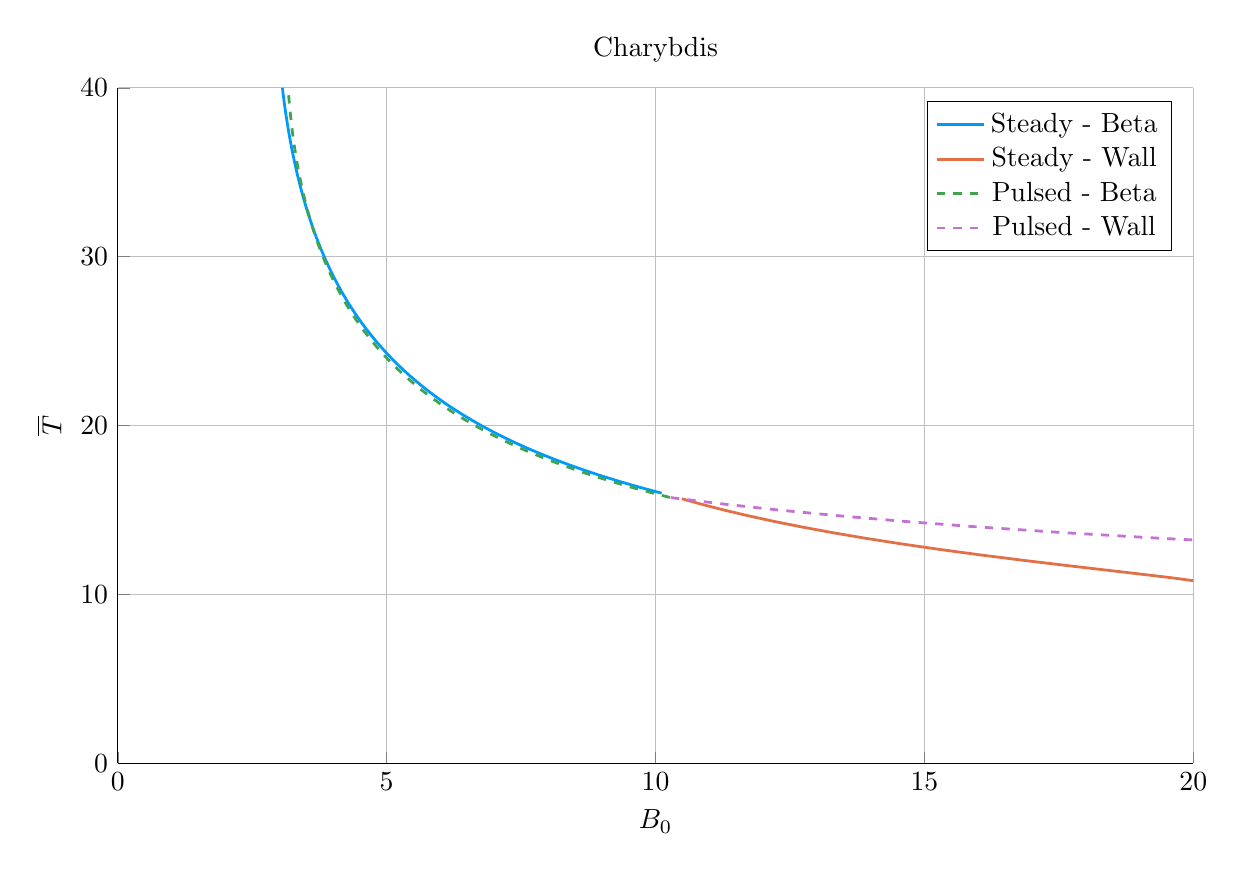
\begin{tikzpicture}[]
\begin{axis}[height = {101.6mm}, ylabel = {$\overline {T}$}, title = {Charybdis}, xmin = {0.0}, xmax = {20.0}, ymax = {40.0}, xlabel = {${B}_{0}$}, {unbounded coords=jump, scaled x ticks = false, xticklabel style={rotate = 0}, xmajorgrids = true, xtick = {0.0,5.0,10.0,15.0,20.0}, xticklabels = {0,5,10,15,20}, xtick align = inside, axis lines* = left, scaled y ticks = false, yticklabel style={rotate = 0}, ymajorgrids = true, ytick = {0.0,10.0,20.0,30.0,40.0}, yticklabels = {0,10,20,30,40}, ytick align = inside, axis lines* = left,     xshift = 0.0mm,
    yshift = 0.0mm,
    axis background/.style={fill={rgb,1:red,1.00000000;green,1.00000000;blue,1.00000000}}
, colorbar style={title=}}, ymin = {0.0}, width = {152.4mm}]\addplot+ [color = {rgb,1:red,0.00000000;green,0.60560316;blue,0.97868012},
draw opacity=1.0,
line width=1,
solid,mark = none,
mark size = 2.0,
mark options = {
    color = {rgb,1:red,0.00000000;green,0.00000000;blue,0.00000000}, draw opacity = 1.0,
    fill = {rgb,1:red,0.00000000;green,0.60560316;blue,0.97868012}, fill opacity = 1.0,
    line width = 1,
    rotate = 0,
    solid
}]coordinates {
(10.112818033153026, 16.0)
(9.722156888543116, 16.333333333333332)
(9.357875603858393, 16.666666666666668)
(9.017653755630063, 17.0)
(8.6995124437054, 17.333333333333332)
(8.401566530516865, 17.666666666666668)
(8.122163706328223, 18.0)
(7.859819415455661, 18.333333333333332)
(7.613196557650265, 18.666666666666668)
(7.381088038653343, 19.0)
(7.162401716104116, 19.333333333333332)
(6.956147367527331, 19.666666666666668)
(6.761425371986388, 20.0)
(6.577416849463348, 20.333333333333332)
(6.403375044688587, 20.666666666666668)
(6.2386177769852695, 21.0)
(6.0825208065966905, 21.333333333333332)
(5.934511989185341, 21.666666666666668)
(5.794066116682695, 22.0)
(5.660700347012839, 22.333333333333332)
(5.533970150598111, 22.666666666666668)
(5.413465705416883, 23.0)
(5.298808685607224, 23.333333333333332)
(5.189649392059402, 23.666666666666668)
(5.085664187259174, 24.0)
(4.986553195072601, 24.333333333333332)
(4.892038235455667, 24.666666666666668)
(4.801860966679364, 25.0)
(4.7157812114040425, 25.333333333333332)
(4.633575445956479, 25.666666666666668)
(4.5550354347559185, 26.0)
(4.479966994069385, 26.333333333333332)
(4.408188871204256, 26.666666666666668)
(4.33953172691477, 27.0)
(4.273837210246432, 27.333333333333332)
(4.210957116299974, 27.666666666666668)
(4.15075261849161, 28.0)
(4.0930935678432965, 28.333333333333332)
(4.037857852672517, 28.666666666666668)
(3.9849308127842145, 29.0)
(3.9342047029103653, 29.333333333333332)
(3.8855782007091695, 29.666666666666668)
(3.838955955133626, 30.0)
(3.7942481714200484, 30.333333333333332)
(3.7513702293348077, 30.666666666666668)
(3.710242331663442, 31.0)
(3.6707891802306123, 31.333333333333332)
(3.6329396770109583, 31.666666666666668)
(3.5966266481325166, 32.0)
(3.5617865887889004, 32.333333333333336)
(3.5283594272686503, 32.666666666666664)
(3.496288306480746, 33.0)
(3.465519381509793, 33.333333333333336)
(3.4360016318699595, 33.666666666666664)
(3.4076866872513096, 34.0)
(3.380528665662031, 34.333333333333336)
(3.3544840229690007, 34.666666666666664)
(3.3295114129297314, 35.0)
(3.3055715568879336, 35.333333333333336)
(3.2826271223788512, 35.666666666666664)
(3.260642607548369, 36.0)
(3.239584247604666, 36.333333333333336)
(3.2194198921826622, 36.666666666666664)
(3.2001189373344725, 37.0)
(3.181652227422265, 37.333333333333336)
(3.163991977015565, 37.666666666666664)
(3.1471116955378684, 38.0)
(3.130986116696265, 38.333333333333336)
(3.115591132350856, 38.666666666666664)
(3.1009037305081053, 39.0)
(3.0869019371473265, 39.333333333333336)
(3.0735647616124355, 39.666666666666664)
(3.0608721453218655, 40.0)
};
\addlegendentry{Steady - Beta}
\addplot+ [color = {rgb,1:red,0.88887350;green,0.43564919;blue,0.27812294},
draw opacity=1.0,
line width=1,
solid,mark = none,
mark size = 2.0,
mark options = {
    color = {rgb,1:red,0.00000000;green,0.00000000;blue,0.00000000}, draw opacity = 1.0,
    fill = {rgb,1:red,0.88887350;green,0.43564919;blue,0.27812294}, fill opacity = 1.0,
    line width = 1,
    rotate = 0,
    solid
}]coordinates {
(20.758867641064707, 10.333333333333334)
(20.346250098246923, 10.666666666666666)
(19.57104597888471, 11.0)
(18.681781921115476, 11.333333333333334)
(17.775790175980152, 11.666666666666666)
(16.896654716492492, 12.0)
(16.063927450323227, 12.333333333333334)
(15.285557510665852, 12.666666666666666)
(14.563500533069154, 13.0)
(13.896568848875791, 13.333333333333334)
(13.281970890030232, 13.666666666666666)
(12.716170469467318, 14.0)
(12.195372283741088, 14.333333333333334)
(11.715794270833433, 14.666666666666666)
(11.273815669498969, 15.0)
(10.866051794088186, 15.333333333333334)
(10.489365023931143, 15.666666666666666)
};
\addlegendentry{Steady - Wall}
\addplot+ [color = {rgb,1:red,0.24222430;green,0.64327509;blue,0.30444865},
draw opacity=1.0,
line width=1,
dashed,mark = none,
mark size = 2.0,
mark options = {
    color = {rgb,1:red,0.00000000;green,0.00000000;blue,0.00000000}, draw opacity = 1.0,
    fill = {rgb,1:red,0.24222430;green,0.64327509;blue,0.30444865}, fill opacity = 1.0,
    line width = 1,
    rotate = 0,
    solid
}]coordinates {
(10.26788634689966, 15.745469117405404)
(9.953967652326213, 16.0)
(9.567926244368271, 16.333333333333332)
(9.207974394987358, 16.666666666666668)
(8.871841888699304, 17.0)
(8.557505525932248, 17.333333333333332)
(8.263156925406376, 17.666666666666668)
(7.9871752024348766, 18.0)
(7.728103682045175, 18.333333333333332)
(7.484629973620137, 18.666666666666668)
(7.255568856523303, 19.0)
(7.039847526735421, 19.333333333333332)
(6.836492834698909, 19.666666666666668)
(6.644620209081183, 20.0)
(6.463424013335149, 20.333333333333332)
(6.2921691243175495, 20.666666666666668)
(6.13018355681404, 21.0)
(5.97685198655569, 21.333333333333332)
(5.831610044919842, 21.666666666666668)
(5.693939286027163, 22.0)
(5.563362729090489, 22.333333333333332)
(5.439440906144732, 22.666666666666668)
(5.321768347746793, 23.0)
(5.209970453003084, 23.333333333333332)
(5.103700692769835, 23.666666666666668)
(5.002638109938164, 24.0)
(4.906485077678376, 24.333333333333332)
(4.814965286571576, 24.666666666666668)
(4.727821933804548, 25.0)
(4.644816091323922, 25.333333333333332)
(4.565725232806084, 25.666666666666668)
(4.490341901840154, 26.0)
(4.418472505906755, 26.333333333333332)
(4.349936222622964, 26.666666666666668)
(4.284564006352339, 27.0)
(4.222197684694192, 27.333333333333332)
(4.162689135592264, 27.666666666666668)
(4.105899536872315, 28.0)
(4.051698680949713, 28.333333333333332)
(3.9999643482627323, 28.666666666666668)
(3.9505817337017928, 29.0)
(3.903442920928527, 29.333333333333332)
(3.858446400032002, 29.666666666666668)
(3.8154966244515616, 30.0)
(3.7745036035252744, 30.333333333333332)
(3.7353825273991994, 30.666666666666668)
(3.6980534213689746, 31.0)
(3.6624408270205375, 31.333333333333332)
(3.62847350780097, 31.666666666666668)
(3.5960841768845415, 32.0)
(3.565209245407392, 32.333333333333336)
(3.5357885893311605, 32.666666666666664)
(3.5077653333614305, 33.0)
(3.4810856504959875, 33.333333333333336)
(3.4556985759109375, 33.666666666666664)
(3.4315558340122845, 34.0)
(3.408611677587535, 34.333333333333336)
(3.3868227380888998, 34.666666666666664)
(3.36614788616562, 35.0)
(3.3465481016421226, 35.333333333333336)
(3.327986352208224, 35.666666666666664)
(3.3104274769652595, 36.0)
(3.2938380965241474, 36.333333333333336)
(3.278186482171801, 36.666666666666664)
(3.263442495132517, 37.0)
(3.2495774839156075, 37.333333333333336)
(3.236564206241785, 37.666666666666664)
(3.224376752844934, 38.0)
(3.212990475972638, 38.333333333333336)
(3.2023819222517877, 38.666666666666664)
(3.192528769611062, 39.0)
(3.1834097679780142, 39.333333333333336)
(3.1750046834890777, 39.666666666666664)
(3.1672942459724482, 40.0)
};
\addlegendentry{Pulsed - Beta}
\addplot+ [color = {rgb,1:red,0.76444018;green,0.44411178;blue,0.82429754},
draw opacity=1.0,
line width=1,
dashed,mark = none,
mark size = 2.0,
mark options = {
    color = {rgb,1:red,0.00000000;green,0.00000000;blue,0.00000000}, draw opacity = 1.0,
    fill = {rgb,1:red,0.76444018;green,0.44411178;blue,0.82429754}, fill opacity = 1.0,
    line width = 1,
    rotate = 0,
    solid
}]coordinates {
(48.990476413653056, 10.666666666666666)
(42.83950920694117, 11.0)
(37.687790427214495, 11.333333333333334)
(33.33937742845888, 11.666666666666666)
(29.64296398154308, 12.0)
(26.48039367255613, 12.333333333333334)
(23.758442882319894, 12.666666666666666)
(21.402860298405816, 13.0)
(19.353987387634486, 13.333333333333334)
(17.563502020363714, 13.666666666666666)
(15.991970371213752, 14.0)
(14.606987499719377, 14.333333333333334)
(13.381751501116137, 14.666666666666666)
(12.293960329570087, 15.0)
(11.32495111804522, 15.333333333333334)
(10.459023415380802, 15.666666666666666)
(10.26788634689966, 15.745469117405404)
};
\addlegendentry{Pulsed - Wall}
\end{axis}

\end{tikzpicture}

    \end{adjustbox}
        \caption{Charybdis}
    \end{subfigure}
    \hfill
    \begin{subfigure}[t]{0.45\textwidth}
        \centering
    \begin{adjustbox}{width=\textwidth}
      \Large
      \begin{tikzpicture}[]
\begin{axis}[height = {101.6mm}, ylabel = {$\overline {T}$}, title = {Proteus}, xmin = {0.0}, xmax = {20.0}, ymax = {40.0}, xlabel = {${B}_{0}$}, {unbounded coords=jump, scaled x ticks = false, xticklabel style={rotate = 0}, xmajorgrids = true, xtick = {0.0,5.0,10.0,15.0,20.0}, xticklabels = {0,5,10,15,20}, xtick align = inside, axis lines* = left, scaled y ticks = false, yticklabel style={rotate = 0}, ymajorgrids = true, ytick = {0.0,10.0,20.0,30.0,40.0}, yticklabels = {0,10,20,30,40}, ytick align = inside, axis lines* = left,     xshift = 0.0mm,
    yshift = 0.0mm,
    axis background/.style={fill={rgb,1:red,1.00000000;green,1.00000000;blue,1.00000000}}
, colorbar style={title=}}, ymin = {0.0}, width = {152.4mm}]\addplot+ [color = {rgb,1:red,0.00000000;green,0.60560316;blue,0.97868012},
draw opacity=1.0,
line width=1,
solid,mark = none,
mark size = 2.0,
mark options = {
    color = {rgb,1:red,0.00000000;green,0.00000000;blue,0.00000000}, draw opacity = 1.0,
    fill = {rgb,1:red,0.00000000;green,0.60560316;blue,0.97868012}, fill opacity = 1.0,
    line width = 1,
    rotate = 0,
    solid
}]coordinates {
(4.658732060637907, 3.3333333333333335)
(4.211109766361548, 3.6666666666666665)
(3.9293920326356777, 4.0)
(3.7651903683456465, 4.333333333333333)
(3.6776039543745567, 4.666666666666667)
(3.6402437753208394, 5.0)
(3.6366994671255806, 5.333333333333333)
(3.656621534643579, 5.666666666666667)
(3.693300156736026, 6.0)
(3.7422515017241134, 6.333333333333333)
(3.865532743079537, 7.0)
(3.936096932264377, 7.333333333333333)
(4.010907188015084, 7.666666666666667)
(4.089072356933184, 8.0)
(4.169903401491354, 8.333333333333334)
(4.252857906625248, 8.666666666666666)
(4.337501757261618, 9.0)
(4.42348218754058, 9.333333333333334)
(4.5983381267510195, 10.0)
(4.686766232902671, 10.333333333333334)
(4.775618142770625, 10.666666666666666)
(4.864743502376605, 11.0)
(4.927312314219091, 11.23366590283607)
};
\addlegendentry{Pulsed - Kink}
\addplot+ [color = {rgb,1:red,0.88887350;green,0.43564919;blue,0.27812294},
draw opacity=1.0,
line width=1,
solid,mark = none,
mark size = 2.0,
mark options = {
    color = {rgb,1:red,0.00000000;green,0.00000000;blue,0.00000000}, draw opacity = 1.0,
    fill = {rgb,1:red,0.88887350;green,0.43564919;blue,0.27812294}, fill opacity = 1.0,
    line width = 1,
    rotate = 0,
    solid
}]coordinates {
(4.927312314219091, 11.23366590283607)
(4.984545814413324, 11.333333333333334)
(5.17452482724068, 11.666666666666666)
(5.362091669637646, 12.0)
(5.54700293215903, 12.333333333333334)
(5.729042482638278, 12.666666666666666)
(5.908022832274664, 13.0)
(6.083785777786694, 13.333333333333334)
(6.256202341425288, 13.666666666666666)
(6.324169421042356, 13.799922978615482)
};
\addlegendentry{Pulsed - Beta}
\addplot+ [color = {rgb,1:red,0.24222430;green,0.64327509;blue,0.30444865},
draw opacity=1.0,
line width=1,
solid,mark = none,
mark size = 2.0,
mark options = {
    color = {rgb,1:red,0.00000000;green,0.00000000;blue,0.00000000}, draw opacity = 1.0,
    fill = {rgb,1:red,0.24222430;green,0.64327509;blue,0.30444865}, fill opacity = 1.0,
    line width = 1,
    rotate = 0,
    solid
}]coordinates {
(6.324169421042356, 13.799922978615482)
(6.727338549778396, 14.0)
(7.320469048424473, 14.333333333333334)
(7.835746509376305, 14.666666666666666)
(8.290245520072391, 15.0)
(8.696162676727877, 15.333333333333334)
(9.0624397222742, 15.666666666666666)
(9.395798186463841, 16.0)
(9.701405747258567, 16.333333333333332)
(10.244760202900984, 17.0)
(10.930275827723788, 18.0)
(11.131878682735255, 18.333333333333332)
(11.50278450645086, 19.0)
(11.83715172742864, 19.666666666666668)
(11.992609772603878, 20.0)
(12.141110720831467, 20.333333333333332)
};
\addlegendentry{Pulsed - Wall}
\end{axis}

\end{tikzpicture}

    \end{adjustbox}
        \caption{Proteus}
    \end{subfigure}
    \hfill \hfill ~\\ ~\\ ~\\ ~\\
    \hfill
    \begin{subfigure}[t]{0.45\textwidth}
        \centering
    \begin{adjustbox}{width=\textwidth}
      \Large
      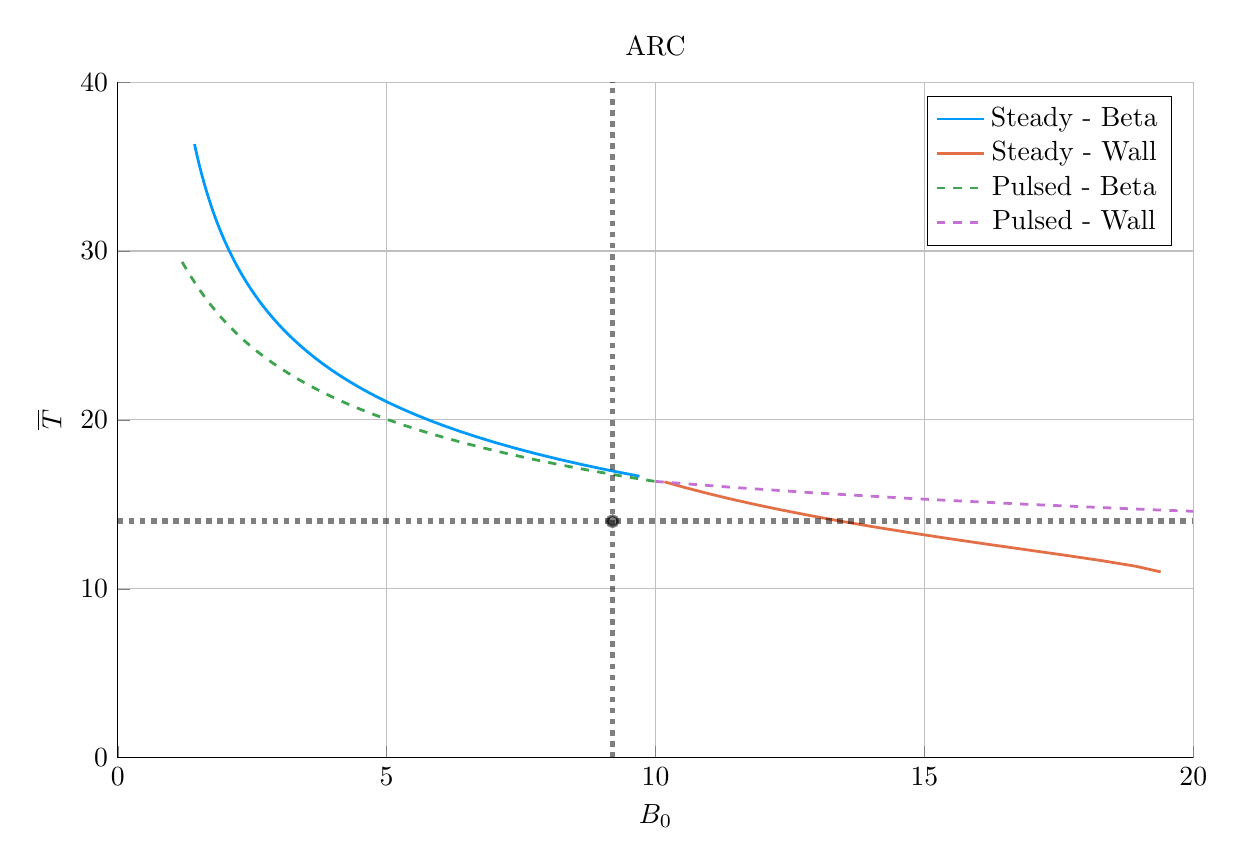
\begin{tikzpicture}[]
\begin{axis}[height = {101.6mm}, ylabel = {$\overline {T}$}, title = {ARC}, xmin = {0.0}, xmax = {20.0}, ymax = {40.0}, xlabel = {${B}_{0}$}, {unbounded coords=jump, scaled x ticks = false, xticklabel style={rotate = 0}, xmajorgrids = true, xtick = {0.0,5.0,10.0,15.0,20.0}, xticklabels = {0,5,10,15,20}, xtick align = inside, axis lines* = left, scaled y ticks = false, yticklabel style={rotate = 0}, ymajorgrids = true, ytick = {0.0,10.0,20.0,30.0,40.0}, yticklabels = {0,10,20,30,40}, ytick align = inside, axis lines* = left,     xshift = 0.0mm,
    yshift = 0.0mm,
    axis background/.style={fill={rgb,1:red,1.00000000;green,1.00000000;blue,1.00000000}}
, colorbar style={title=}}, ymin = {0.0}, width = {152.4mm}]\addplot+ [color = {rgb,1:red,0.00000000;green,0.60560316;blue,0.97868012},
draw opacity=1.0,
line width=1,
solid,mark = none,
mark size = 2.0,
mark options = {
    color = {rgb,1:red,0.00000000;green,0.00000000;blue,0.00000000}, draw opacity = 1.0,
    fill = {rgb,1:red,0.00000000;green,0.60560316;blue,0.97868012}, fill opacity = 1.0,
    line width = 1,
    rotate = 0,
    solid
}]coordinates {
(9.701206080853105, 16.666666666666668)
(9.162315904693079, 17.0)
(8.664301107137337, 17.333333333333332)
(8.203576462497304, 17.666666666666668)
(7.776718537485166, 18.0)
(7.380720231870917, 18.333333333333332)
(7.012886014999712, 18.666666666666668)
(6.670795005901889, 19.0)
(6.352268997292712, 19.333333333333332)
(6.055344682097163, 19.666666666666668)
(5.778249464564785, 20.0)
(5.519380338856715, 20.333333333333332)
(5.2772854007125325, 20.666666666666668)
(5.050647625972996, 21.0)
(4.838270606140816, 21.333333333333332)
(4.639065978019038, 21.666666666666668)
(4.4520423235376105, 22.0)
(4.276295348572609, 22.333333333333332)
(4.110999177018484, 22.666666666666668)
(3.9553986195015125, 23.0)
(3.8088022956698633, 23.333333333333332)
(3.6705765055641186, 23.666666666666668)
(3.54013975965751, 24.0)
(3.4169578891619192, 24.333333333333332)
(3.30053966845824, 24.666666666666668)
(3.1904328903033052, 25.0)
(3.086220842019516, 25.333333333333332)
(2.9875191373772063, 25.666666666666668)
(2.8939728644914635, 26.0)
(2.8052540149097247, 26.333333333333332)
(2.7210591632720242, 26.666666666666668)
(2.6411073705789065, 27.0)
(2.565138287279709, 27.333333333333332)
(2.492910435164382, 27.666666666666668)
(2.4241996494611984, 28.0)
(2.3587976646588236, 28.333333333333332)
(2.296510829425685, 28.666666666666668)
(2.237158937627476, 29.0)
(2.180574163874242, 29.333333333333332)
(2.126600093288366, 29.666666666666668)
(2.075090836295778, 30.0)
(2.0259102202234582, 30.333333333333332)
(1.978931050353818, 30.666666666666668)
(1.9340344338545452, 31.0)
(1.8911091606836798, 31.333333333333332)
(1.8500511361739687, 31.666666666666668)
(1.8107628605384507, 32.0)
(1.773152951016952, 32.333333333333336)
(1.7371357028100902, 32.666666666666664)
(1.7026306853269466, 33.0)
(1.6695623706125668, 33.333333333333336)
(1.6378597911249178, 33.666666666666664)
(1.607456224302725, 34.0)
(1.5782889016090462, 34.333333333333336)
(1.5502987399539199, 34.666666666666664)
(1.5234300935954943, 35.0)
(1.4976305247952577, 35.333333333333336)
(1.4728505916614916, 35.666666666666664)
(1.4490436517578602, 36.0)
(1.4261656801829077, 36.333333333333336)
};
\addlegendentry{Steady - Beta}
\addplot+ [color = {rgb,1:red,0.88887350;green,0.43564919;blue,0.27812294},
draw opacity=1.0,
line width=1,
solid,mark = none,
mark size = 2.0,
mark options = {
    color = {rgb,1:red,0.00000000;green,0.00000000;blue,0.00000000}, draw opacity = 1.0,
    fill = {rgb,1:red,0.88887350;green,0.43564919;blue,0.27812294}, fill opacity = 1.0,
    line width = 1,
    rotate = 0,
    solid
}]coordinates {
(19.394007482712425, 11.0)
(18.932196567189358, 11.333333333333334)
(18.296989378345195, 11.666666666666666)
(17.587029315408756, 12.0)
(16.847882407994106, 12.333333333333334)
(16.111374502564406, 12.666666666666666)
(15.396027314547156, 13.0)
(14.710952688793137, 13.333333333333334)
(14.06168447794857, 13.666666666666666)
(13.450465418483889, 14.0)
(12.877644538645335, 14.333333333333334)
(12.342394470642008, 14.666666666666666)
(11.843182246608265, 15.0)
(11.376441269625893, 15.333333333333334)
(10.944966372727551, 15.666666666666666)
(10.541663878705513, 16.0)
(10.165908182236457, 16.333333333333332)
};
\addlegendentry{Steady - Wall}
\addplot+ [color = {rgb,1:red,0.24222430;green,0.64327509;blue,0.30444865},
draw opacity=1.0,
line width=1,
dashed,mark = none,
mark size = 2.0,
mark options = {
    color = {rgb,1:red,0.00000000;green,0.00000000;blue,0.00000000}, draw opacity = 1.0,
    fill = {rgb,1:red,0.24222430;green,0.64327509;blue,0.30444865}, fill opacity = 1.0,
    line width = 1,
    rotate = 0,
    solid
}]coordinates {
(9.980483622051658, 16.364160609330686)
(9.392786903460065, 16.666666666666668)
(8.79273598103983, 17.0)
(8.23820290909994, 17.333333333333332)
(7.725182218401588, 17.666666666666668)
(7.250078106370205, 18.0)
(6.80965553466646, 18.333333333333332)
(6.400998063035608, 18.666666666666668)
(6.0214713600430425, 19.0)
(5.668691517461799, 19.333333333333332)
(5.340497445229901, 19.666666666666668)
(5.034926745580058, 20.0)
(4.750194564008521, 20.333333333333332)
(4.484674995755211, 20.666666666666668)
(4.236884692979903, 21.0)
(4.00546837264544, 21.333333333333332)
(3.7891859704718387, 21.666666666666668)
(3.5869012239550364, 22.0)
(3.3975714987448393, 22.333333333333332)
(3.2202386987489797, 22.666666666666668)
(3.0540211220494466, 23.0)
(2.8981061427709687, 23.333333333333332)
(2.7517436139566023, 23.666666666666668)
(2.6142398986781377, 24.0)
(2.4849524463010138, 24.333333333333332)
(2.363284838174807, 24.666666666666668)
(2.248682232019848, 25.0)
(2.140627136740878, 25.333333333333332)
(2.038635448877246, 25.666666666666668)
(1.9422526775794744, 26.0)
(1.8510502754751532, 26.333333333333332)
(1.7646219756564088, 26.666666666666668)
(1.6825800061969869, 27.0)
(1.6045510059627948, 27.333333333333332)
(1.53017138625397, 27.666666666666668)
(1.4590817483192686, 28.0)
(1.3909197311384796, 28.333333333333332)
(1.3253102336217724, 28.666666666666668)
(1.261851128383913, 29.0)
(1.20009089049112, 29.333333333333332)
(1.1394908096975784, 29.666666666666668)
};
\addlegendentry{Pulsed - Beta}
\addplot+ [color = {rgb,1:red,0.76444018;green,0.44411178;blue,0.82429754},
draw opacity=1.0,
line width=1,
dashed,mark = none,
mark size = 2.0,
mark options = {
    color = {rgb,1:red,0.00000000;green,0.00000000;blue,0.00000000}, draw opacity = 1.0,
    fill = {rgb,1:red,0.76444018;green,0.44411178;blue,0.82429754}, fill opacity = 1.0,
    line width = 1,
    rotate = 0,
    solid
}]coordinates {
(29.27715761652869, 13.666666666666666)
(25.4410619834368, 14.0)
(22.158819835998365, 14.333333333333334)
(19.342453256965573, 14.666666666666666)
(16.919364280634177, 15.0)
(14.829378672669455, 15.333333333333334)
(13.022412368922526, 15.666666666666666)
(11.456617692058645, 16.0)
(10.096901921254785, 16.333333333333332)
(9.980483622051658, 16.364160609330686)
};
\addlegendentry{Pulsed - Wall}
\addplot+ [color = {rgb,1:red,0.00000000;green,0.00000000;blue,0.00000000},
draw opacity=0.5,
line width=2,
dotted,mark = none,
mark size = 2.0,
mark options = {
    color = {rgb,1:red,0.00000000;green,0.00000000;blue,0.00000000}, draw opacity = 0.5,
    fill = {rgb,1:red,0.00000000;green,0.00000000;blue,0.00000000}, fill opacity = 0.5,
    line width = 1,
    rotate = 0,
    solid
},forget plot]coordinates {
(0.0, 14.0)
(20.0, 14.0)
};
\addplot+ [color = {rgb,1:red,0.00000000;green,0.00000000;blue,0.00000000},
draw opacity=0.5,
line width=2,
dotted,mark = none,
mark size = 2.0,
mark options = {
    color = {rgb,1:red,0.00000000;green,0.00000000;blue,0.00000000}, draw opacity = 0.5,
    fill = {rgb,1:red,0.00000000;green,0.00000000;blue,0.00000000}, fill opacity = 0.5,
    line width = 1,
    rotate = 0,
    solid
},forget plot]coordinates {
(9.2, 0.0)
(9.2, 40.0)
};
\addplot+[draw=none, color = {rgb,1:red,0.00000000;green,0.00000000;blue,0.00000000},
draw opacity=0.5,
line width=0,
solid,mark = *,
mark size = 2.0,
mark options = {
    color = {rgb,1:red,0.00000000;green,0.00000000;blue,0.00000000}, draw opacity = 0.5,
    fill = {rgb,1:red,0.00000000;green,0.00000000;blue,0.00000000}, fill opacity = 0.5,
    line width = 1,
    rotate = 0,
    solid
},forget plot] coordinates {
(9.2, 14.0)
};
\end{axis}

\end{tikzpicture}

    \end{adjustbox}
        \caption{ARC}
    \end{subfigure}
    \hfill
    \begin{subfigure}[t]{0.45\textwidth}
        \centering
    \begin{adjustbox}{width=\textwidth}
      \Large
      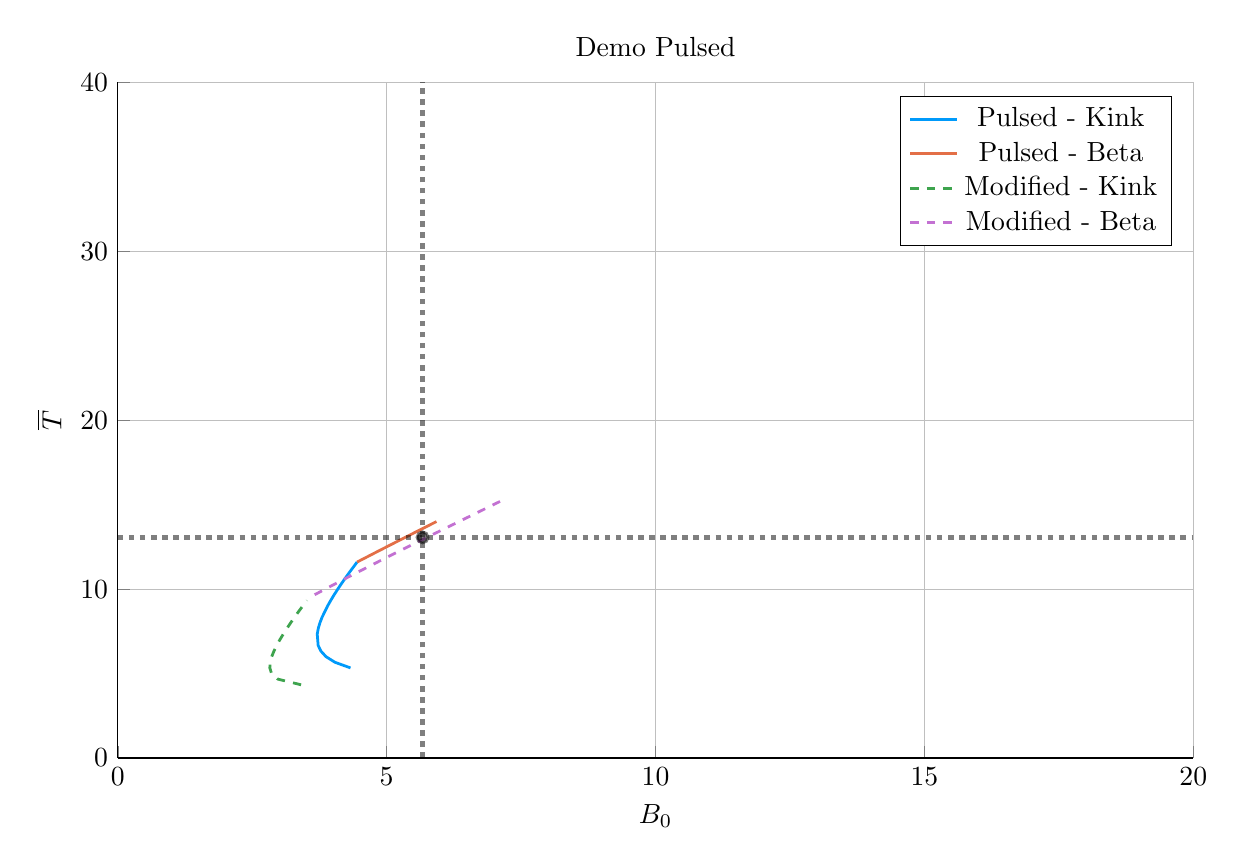
\begin{tikzpicture}[]
\begin{axis}[height = {101.6mm}, ylabel = {$\overline {T}$}, title = {Demo Pulsed}, xmin = {0.0}, xmax = {20.0}, ymax = {40.0}, xlabel = {${B}_{0}$}, {unbounded coords=jump, scaled x ticks = false, xticklabel style={rotate = 0}, xmajorgrids = true, xtick = {0.0,5.0,10.0,15.0,20.0}, xticklabels = {0,5,10,15,20}, xtick align = inside, axis lines* = left, scaled y ticks = false, yticklabel style={rotate = 0}, ymajorgrids = true, ytick = {0.0,10.0,20.0,30.0,40.0}, yticklabels = {0,10,20,30,40}, ytick align = inside, axis lines* = left,     xshift = 0.0mm,
    yshift = 0.0mm,
    axis background/.style={fill={rgb,1:red,1.00000000;green,1.00000000;blue,1.00000000}}
, colorbar style={title=}}, ymin = {0.0}, width = {152.4mm}]\addplot+ [color = {rgb,1:red,0.00000000;green,0.60560316;blue,0.97868012},
draw opacity=1.0,
line width=1,
solid,mark = none,
mark size = 2.0,
mark options = {
    color = {rgb,1:red,0.00000000;green,0.00000000;blue,0.00000000}, draw opacity = 1.0,
    fill = {rgb,1:red,0.00000000;green,0.60560316;blue,0.97868012}, fill opacity = 1.0,
    line width = 1,
    rotate = 0,
    solid
}]coordinates {
(4.327031075670194, 5.333333333333333)
(4.038214026054326, 5.666666666666667)
(3.8713719163129245, 6.0)
(3.7758613845615545, 6.333333333333333)
(3.7257856761317214, 6.666666666666667)
(3.7090473695925437, 7.333333333333333)
(3.727711597554826, 7.666666666666667)
(3.7586131667481433, 8.0)
(3.799052518631718, 8.333333333333334)
(3.901290136389271, 9.0)
(3.960577465316514, 9.333333333333334)
(4.0241209645210345, 9.666666666666666)
(4.0912717805663785, 10.0)
(4.161514602943343, 10.333333333333334)
(4.2344343960723005, 10.666666666666666)
(4.309692554546368, 11.0)
(4.450417240491067, 11.600962879632572)
};
\addlegendentry{Pulsed - Kink}
\addplot+ [color = {rgb,1:red,0.88887350;green,0.43564919;blue,0.27812294},
draw opacity=1.0,
line width=1,
solid,mark = none,
mark size = 2.0,
mark options = {
    color = {rgb,1:red,0.00000000;green,0.00000000;blue,0.00000000}, draw opacity = 1.0,
    fill = {rgb,1:red,0.88887350;green,0.43564919;blue,0.27812294}, fill opacity = 1.0,
    line width = 1,
    rotate = 0,
    solid
}]coordinates {
(4.450417240491067, 11.600962879632572)
(4.490148631384312, 11.666666666666666)
(4.692490181445514, 12.0)
(4.8960344619053355, 12.333333333333334)
(5.100651132702229, 12.666666666666666)
(5.306202822090688, 13.0)
(5.512545696627038, 13.333333333333334)
(5.719530043226767, 13.666666666666666)
(5.927000883375481, 14.0)
};
\addlegendentry{Pulsed - Beta}
\addplot+ [color = {rgb,1:red,0.24222430;green,0.64327509;blue,0.30444865},
draw opacity=1.0,
line width=1,
dashed,mark = none,
mark size = 2.0,
mark options = {
    color = {rgb,1:red,0.00000000;green,0.00000000;blue,0.00000000}, draw opacity = 1.0,
    fill = {rgb,1:red,0.24222430;green,0.64327509;blue,0.30444865}, fill opacity = 1.0,
    line width = 1,
    rotate = 0,
    solid
}]coordinates {
(3.4087424183072135, 4.333333333333333)
(2.977074181068944, 4.666666666666667)
(2.8592500074202523, 5.0)
(2.827199220063259, 5.333333333333333)
(2.8339789008667826, 5.666666666666667)
(2.862412302880871, 6.0)
(2.9044598258085443, 6.333333333333333)
(2.95577893007882, 6.666666666666667)
(3.0137895352525907, 7.0)
(3.076849710218805, 7.333333333333333)
(3.1438583711612704, 7.666666666666667)
(3.214045733980633, 8.0)
(3.2868548955983727, 8.333333333333334)
(3.361871149981842, 8.666666666666666)
(3.4387778750377818, 9.0)
(3.5173279629378453, 9.333333333333334)
};
\addlegendentry{Modified - Kink}
\addplot+ [color = {rgb,1:red,0.76444018;green,0.44411178;blue,0.82429754},
draw opacity=1.0,
line width=1,
dashed,mark = none,
mark size = 2.0,
mark options = {
    color = {rgb,1:red,0.00000000;green,0.00000000;blue,0.00000000}, draw opacity = 1.0,
    fill = {rgb,1:red,0.76444018;green,0.44411178;blue,0.82429754}, fill opacity = 1.0,
    line width = 1,
    rotate = 0,
    solid
}]coordinates {
(3.6607028750648505, 9.666666666666666)
(3.8574448036470477, 10.0)
(4.056375867871351, 10.333333333333334)
(4.257366397480293, 10.666666666666666)
(4.460279103534801, 11.0)
(4.664969389370631, 11.333333333333334)
(4.871285596007394, 11.666666666666666)
(5.07906923307514, 12.0)
(5.288155233306219, 12.333333333333334)
(5.498372259673351, 12.666666666666666)
(5.709543087166185, 13.0)
(5.921485076209294, 13.333333333333334)
(6.134010749367255, 13.666666666666666)
(6.346928478632384, 14.0)
(6.560043285872518, 14.333333333333334)
(6.773157754368795, 14.666666666666666)
(6.986073044284746, 15.0)
(7.198590001107076, 15.333333333333334)
};
\addlegendentry{Modified - Beta}
\addplot+ [color = {rgb,1:red,0.00000000;green,0.00000000;blue,0.00000000},
draw opacity=0.5,
line width=2,
dotted,mark = none,
mark size = 2.0,
mark options = {
    color = {rgb,1:red,0.00000000;green,0.00000000;blue,0.00000000}, draw opacity = 0.5,
    fill = {rgb,1:red,0.00000000;green,0.00000000;blue,0.00000000}, fill opacity = 0.5,
    line width = 1,
    rotate = 0,
    solid
},forget plot]coordinates {
(0.0, 13.065)
(20.0, 13.065)
};
\addplot+ [color = {rgb,1:red,0.00000000;green,0.00000000;blue,0.00000000},
draw opacity=0.5,
line width=2,
dotted,mark = none,
mark size = 2.0,
mark options = {
    color = {rgb,1:red,0.00000000;green,0.00000000;blue,0.00000000}, draw opacity = 0.5,
    fill = {rgb,1:red,0.00000000;green,0.00000000;blue,0.00000000}, fill opacity = 0.5,
    line width = 1,
    rotate = 0,
    solid
},forget plot]coordinates {
(5.667, 0.0)
(5.667, 40.0)
};
\addplot+[draw=none, color = {rgb,1:red,0.00000000;green,0.00000000;blue,0.00000000},
draw opacity=0.5,
line width=0,
solid,mark = *,
mark size = 2.0,
mark options = {
    color = {rgb,1:red,0.00000000;green,0.00000000;blue,0.00000000}, draw opacity = 0.5,
    fill = {rgb,1:red,0.00000000;green,0.00000000;blue,0.00000000}, fill opacity = 0.5,
    line width = 1,
    rotate = 0,
    solid
},forget plot] coordinates {
(5.667, 13.065)
};
\end{axis}

\end{tikzpicture}

    \end{adjustbox}
        \caption{DEMO Pulsed}
    \end{subfigure}
    \hfill \hfill ~\\ ~\\ ~\\ ~\\
    \hfill
    \begin{subfigure}[t]{0.45\textwidth}
        \centering
    \begin{adjustbox}{width=\textwidth}
      \Large
      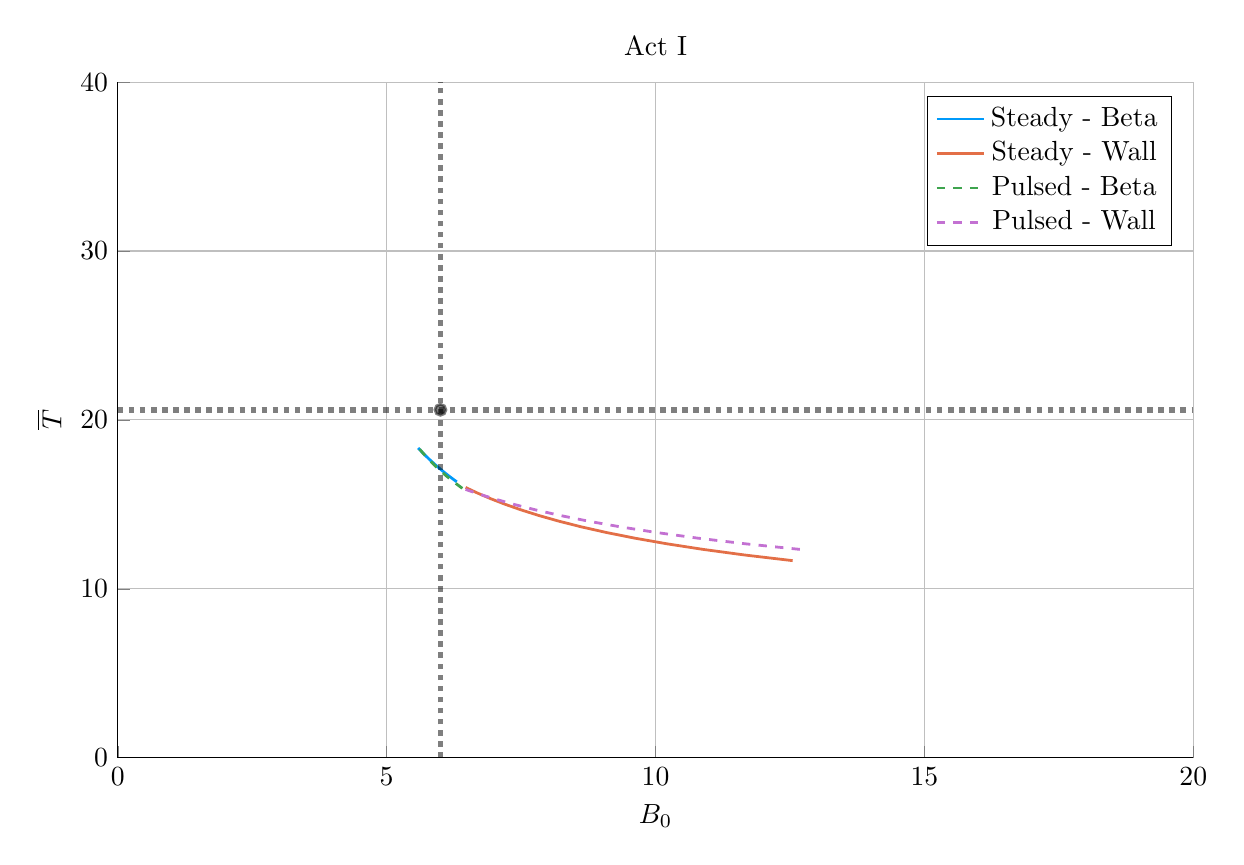
\begin{tikzpicture}[]
\begin{axis}[height = {101.6mm}, ylabel = {$\overline {T}$}, title = {Act I}, xmin = {0.0}, xmax = {20.0}, ymax = {40.0}, xlabel = {${B}_{0}$}, {unbounded coords=jump, scaled x ticks = false, xticklabel style={rotate = 0}, xmajorgrids = true, xtick = {0.0,5.0,10.0,15.0,20.0}, xticklabels = {0,5,10,15,20}, xtick align = inside, axis lines* = left, scaled y ticks = false, yticklabel style={rotate = 0}, ymajorgrids = true, ytick = {0.0,10.0,20.0,30.0,40.0}, yticklabels = {0,10,20,30,40}, ytick align = inside, axis lines* = left,     xshift = 0.0mm,
    yshift = 0.0mm,
    axis background/.style={fill={rgb,1:red,1.00000000;green,1.00000000;blue,1.00000000}}
, colorbar style={title=}}, ymin = {0.0}, width = {152.4mm}]\addplot+ [color = {rgb,1:red,0.00000000;green,0.60560316;blue,0.97868012},
draw opacity=1.0,
line width=1,
solid,mark = none,
mark size = 2.0,
mark options = {
    color = {rgb,1:red,0.00000000;green,0.00000000;blue,0.00000000}, draw opacity = 1.0,
    fill = {rgb,1:red,0.00000000;green,0.60560316;blue,0.97868012}, fill opacity = 1.0,
    line width = 1,
    rotate = 0,
    solid
}]coordinates {
(6.30336807958207, 16.333333333333332)
(6.162193069273141, 16.666666666666668)
(6.030717178404645, 17.0)
(5.908065509576601, 17.333333333333332)
(5.793464904530972, 17.666666666666668)
(5.686229631357383, 18.0)
(5.585749511271037, 18.333333333333332)
};
\addlegendentry{Steady - Beta}
\addplot+ [color = {rgb,1:red,0.88887350;green,0.43564919;blue,0.27812294},
draw opacity=1.0,
line width=1,
solid,mark = none,
mark size = 2.0,
mark options = {
    color = {rgb,1:red,0.00000000;green,0.00000000;blue,0.00000000}, draw opacity = 1.0,
    fill = {rgb,1:red,0.88887350;green,0.43564919;blue,0.27812294}, fill opacity = 1.0,
    line width = 1,
    rotate = 0,
    solid
}]coordinates {
(12.549536249695134, 11.666666666666666)
(11.658754653696462, 12.0)
(10.883719833507003, 12.333333333333334)
(10.206258129789394, 12.666666666666666)
(9.611335769312953, 13.0)
(9.086446934250878, 13.333333333333334)
(8.62129895070743, 13.666666666666666)
(8.207216040989662, 14.0)
(7.837119555085499, 14.333333333333334)
(7.505047858717157, 14.666666666666666)
(7.20604322925957, 15.0)
(6.935884710193303, 15.333333333333334)
(6.691016583192173, 15.666666666666666)
(6.468415485086983, 16.0)
};
\addlegendentry{Steady - Wall}
\addplot+ [color = {rgb,1:red,0.24222430;green,0.64327509;blue,0.30444865},
draw opacity=1.0,
line width=1,
dashed,mark = none,
mark size = 2.0,
mark options = {
    color = {rgb,1:red,0.00000000;green,0.00000000;blue,0.00000000}, draw opacity = 1.0,
    fill = {rgb,1:red,0.24222430;green,0.64327509;blue,0.30444865}, fill opacity = 1.0,
    line width = 1,
    rotate = 0,
    solid
}]coordinates {
(6.408263337806559, 15.948125117373092)
(6.408263337806564, 15.9481251173731)
(6.385466513301022, 16.0)
(6.245492502072912, 16.333333333333332)
(6.116010320461132, 16.666666666666668)
(5.9960421481916395, 17.0)
(5.884727159112828, 17.333333333333332)
(5.781304768121868, 17.666666666666668)
(5.685100648450046, 18.0)
(5.595515000321003, 18.333333333333332)
};
\addlegendentry{Pulsed - Beta}
\addplot+ [color = {rgb,1:red,0.76444018;green,0.44411178;blue,0.82429754},
draw opacity=1.0,
line width=1,
dashed,mark = none,
mark size = 2.0,
mark options = {
    color = {rgb,1:red,0.00000000;green,0.00000000;blue,0.00000000}, draw opacity = 1.0,
    fill = {rgb,1:red,0.76444018;green,0.44411178;blue,0.82429754}, fill opacity = 1.0,
    line width = 1,
    rotate = 0,
    solid
}]coordinates {
(12.684248532650473, 12.333333333333334)
(11.66307871570063, 12.666666666666666)
(10.781888309639141, 13.0)
(10.016282491385791, 13.333333333333334)
(9.346943280276514, 13.666666666666666)
(8.758420158941194, 14.0)
(8.238241792953433, 14.333333333333334)
(7.776255600865612, 14.666666666666666)
(7.364131118520045, 15.0)
(6.994982564641668, 15.333333333333334)
(6.66307916140573, 15.666666666666666)
(6.408263337806559, 15.948125117373092)
(6.408263337806564, 15.9481251173731)
};
\addlegendentry{Pulsed - Wall}
\addplot+ [color = {rgb,1:red,0.00000000;green,0.00000000;blue,0.00000000},
draw opacity=0.5,
line width=2,
dotted,mark = none,
mark size = 2.0,
mark options = {
    color = {rgb,1:red,0.00000000;green,0.00000000;blue,0.00000000}, draw opacity = 0.5,
    fill = {rgb,1:red,0.00000000;green,0.00000000;blue,0.00000000}, fill opacity = 0.5,
    line width = 1,
    rotate = 0,
    solid
},forget plot]coordinates {
(0.0, 20.6)
(20.0, 20.6)
};
\addplot+ [color = {rgb,1:red,0.00000000;green,0.00000000;blue,0.00000000},
draw opacity=0.5,
line width=2,
dotted,mark = none,
mark size = 2.0,
mark options = {
    color = {rgb,1:red,0.00000000;green,0.00000000;blue,0.00000000}, draw opacity = 0.5,
    fill = {rgb,1:red,0.00000000;green,0.00000000;blue,0.00000000}, fill opacity = 0.5,
    line width = 1,
    rotate = 0,
    solid
},forget plot]coordinates {
(6.0, 0.0)
(6.0, 40.0)
};
\addplot+[draw=none, color = {rgb,1:red,0.00000000;green,0.00000000;blue,0.00000000},
draw opacity=0.5,
line width=0,
solid,mark = *,
mark size = 2.0,
mark options = {
    color = {rgb,1:red,0.00000000;green,0.00000000;blue,0.00000000}, draw opacity = 0.5,
    fill = {rgb,1:red,0.00000000;green,0.00000000;blue,0.00000000}, fill opacity = 0.5,
    line width = 1,
    rotate = 0,
    solid
},forget plot] coordinates {
(6.0, 20.6)
};
\end{axis}

\end{tikzpicture}

    \end{adjustbox}
        \caption{ACT I}
    \end{subfigure}
    \hfill
    \begin{subfigure}[t]{0.45\textwidth}
        \centering
    \begin{adjustbox}{width=\textwidth}
      \Large
      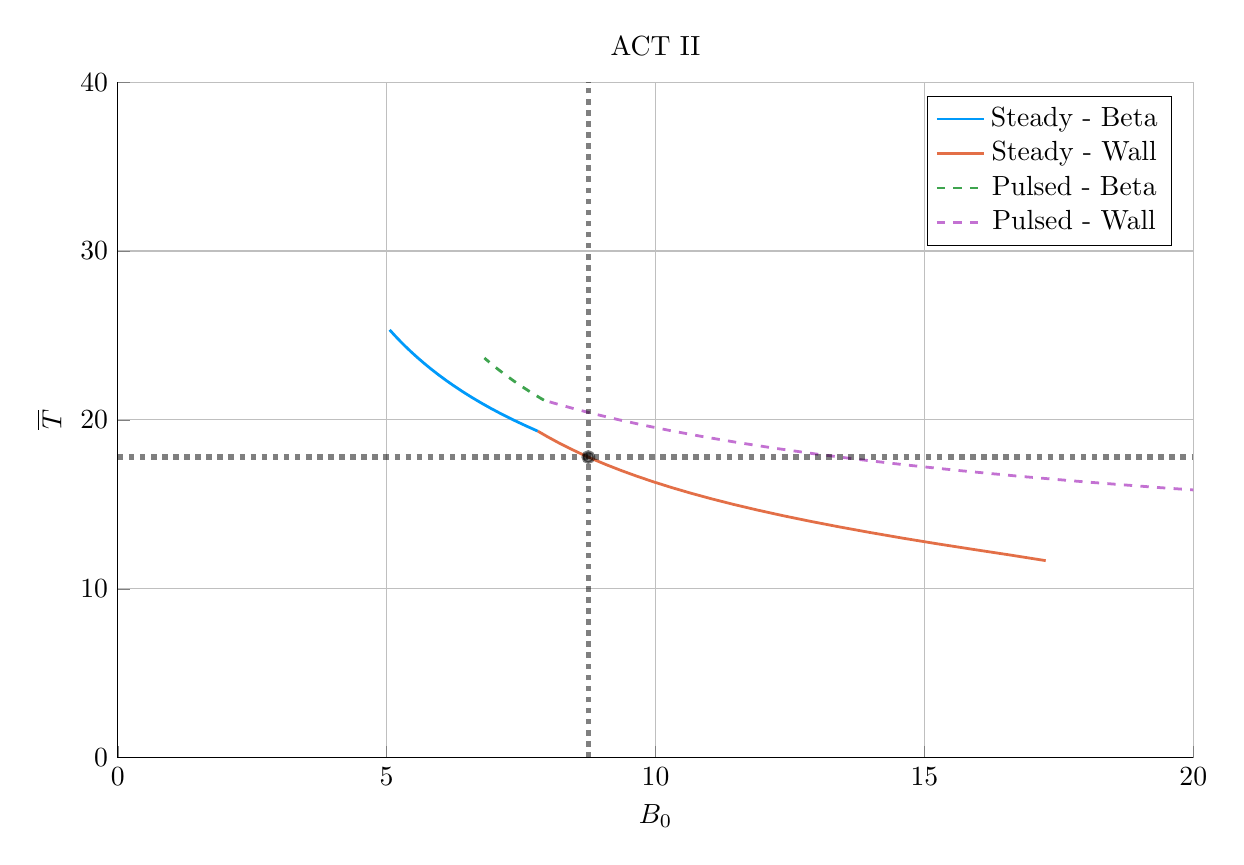
\begin{tikzpicture}[]
\begin{axis}[height = {101.6mm}, ylabel = {$\overline {T}$}, title = {ACT II}, xmin = {0.0}, xmax = {20.0}, ymax = {40.0}, xlabel = {${B}_{0}$}, {unbounded coords=jump, scaled x ticks = false, xticklabel style={rotate = 0}, xmajorgrids = true, xtick = {0.0,5.0,10.0,15.0,20.0}, xticklabels = {0,5,10,15,20}, xtick align = inside, axis lines* = left, scaled y ticks = false, yticklabel style={rotate = 0}, ymajorgrids = true, ytick = {0.0,10.0,20.0,30.0,40.0}, yticklabels = {0,10,20,30,40}, ytick align = inside, axis lines* = left,     xshift = 0.0mm,
    yshift = 0.0mm,
    axis background/.style={fill={rgb,1:red,1.00000000;green,1.00000000;blue,1.00000000}}
, colorbar style={title=}}, ymin = {0.0}, width = {152.4mm}]\addplot+ [color = {rgb,1:red,0.00000000;green,0.60560316;blue,0.97868012},
draw opacity=1.0,
line width=1,
solid,mark = none,
mark size = 2.0,
mark options = {
    color = {rgb,1:red,0.00000000;green,0.00000000;blue,0.00000000}, draw opacity = 1.0,
    fill = {rgb,1:red,0.00000000;green,0.60560316;blue,0.97868012}, fill opacity = 1.0,
    line width = 1,
    rotate = 0,
    solid
}]coordinates {
(7.810935944285959, 19.333333333333332)
(7.57736049850867, 19.666666666666668)
(7.354864292609041, 20.0)
(7.145167234136329, 20.333333333333332)
(6.9473303865083675, 20.666666666666668)
(6.760499508614096, 21.0)
(6.583897990324067, 21.333333333333332)
(6.416817229618043, 21.666666666666668)
(6.258609820663305, 22.0)
(6.108683264880386, 22.333333333333332)
(5.966494431410919, 22.666666666666668)
(5.831544666176381, 23.0)
(5.703375459679132, 23.333333333333332)
(5.581564609582325, 23.666666666666668)
(5.465722802994068, 24.0)
(5.355490573482678, 24.333333333333332)
(5.25053558682053, 24.666666666666668)
(5.1505502068221745, 25.0)
(5.0552493196883175, 25.333333333333332)
};
\addlegendentry{Steady - Beta}
\addplot+ [color = {rgb,1:red,0.88887350;green,0.43564919;blue,0.27812294},
draw opacity=1.0,
line width=1,
solid,mark = none,
mark size = 2.0,
mark options = {
    color = {rgb,1:red,0.00000000;green,0.00000000;blue,0.00000000}, draw opacity = 1.0,
    fill = {rgb,1:red,0.88887350;green,0.43564919;blue,0.27812294}, fill opacity = 1.0,
    line width = 1,
    rotate = 0,
    solid
}]coordinates {
(17.25550839059296, 11.666666666666666)
(16.594334962335296, 12.0)
(15.9071755430688, 12.333333333333334)
(15.233983138507648, 12.666666666666666)
(14.594239858921854, 13.0)
(13.989673082630297, 13.333333333333334)
(13.414782495717416, 13.666666666666666)
(12.872659546281994, 14.0)
(12.364365715508608, 14.333333333333334)
(11.889507953196574, 14.666666666666666)
(11.44685939646348, 15.0)
(11.034739998180656, 15.333333333333334)
(10.651252523287319, 15.666666666666666)
(10.294428800132035, 16.0)
(9.962319203963213, 16.333333333333332)
(9.653045819449929, 16.666666666666668)
(9.364832254395445, 17.0)
(9.096018465506306, 17.333333333333332)
(8.844373144802077, 17.666666666666668)
(8.61055754360846, 18.0)
(8.391192178573277, 18.333333333333332)
(8.18577947665566, 18.666666666666668)
(7.99323348423048, 19.0)
(7.812301489248497, 19.333333333333332)
};
\addlegendentry{Steady - Wall}
\addplot+ [color = {rgb,1:red,0.24222430;green,0.64327509;blue,0.30444865},
draw opacity=1.0,
line width=1,
dashed,mark = none,
mark size = 2.0,
mark options = {
    color = {rgb,1:red,0.00000000;green,0.00000000;blue,0.00000000}, draw opacity = 1.0,
    fill = {rgb,1:red,0.24222430;green,0.64327509;blue,0.30444865}, fill opacity = 1.0,
    line width = 1,
    rotate = 0,
    solid
}]coordinates {
(7.923668284887995, 21.17034352159018)
(7.923668284887995, 21.170343521590212)
(7.836759696043437, 21.333333333333332)
(7.6662731560983355, 21.666666666666668)
(7.50499428233835, 22.0)
(7.35232773269976, 22.333333333333332)
(7.207727224738343, 22.666666666666668)
(7.070690693175276, 23.0)
(6.940756001029682, 23.333333333333332)
(6.817497143644154, 23.666666666666668)
};
\addlegendentry{Pulsed - Beta}
\addplot+ [color = {rgb,1:red,0.76444018;green,0.44411178;blue,0.82429754},
draw opacity=1.0,
line width=1,
dashed,mark = none,
mark size = 2.0,
mark options = {
    color = {rgb,1:red,0.00000000;green,0.00000000;blue,0.00000000}, draw opacity = 1.0,
    fill = {rgb,1:red,0.76444018;green,0.44411178;blue,0.82429754}, fill opacity = 1.0,
    line width = 1,
    rotate = 0,
    solid
}]coordinates {
(22.56106430311702, 15.333333333333334)
(20.85607192394036, 15.666666666666666)
(19.335265246056654, 16.0)
(17.974121547130903, 16.333333333333332)
(16.751976718553127, 16.666666666666668)
(15.651329744019142, 17.0)
(14.65728744097675, 17.333333333333332)
(13.757118584462601, 17.666666666666668)
(12.939893642194303, 18.0)
(12.196191964860315, 18.333333333333332)
(11.517862472405039, 18.666666666666668)
(10.897827027335556, 19.0)
(10.329918077124672, 19.333333333333332)
(9.808743940706389, 19.666666666666668)
(9.329576544487265, 20.0)
(8.888257451278507, 20.333333333333332)
(8.481118883411932, 20.666666666666668)
(8.10491708701527, 21.0)
(7.923668284887995, 21.17034352159018)
(7.923668284887995, 21.170343521590212)
};
\addlegendentry{Pulsed - Wall}
\addplot+ [color = {rgb,1:red,0.00000000;green,0.00000000;blue,0.00000000},
draw opacity=0.5,
line width=2,
dotted,mark = none,
mark size = 2.0,
mark options = {
    color = {rgb,1:red,0.00000000;green,0.00000000;blue,0.00000000}, draw opacity = 0.5,
    fill = {rgb,1:red,0.00000000;green,0.00000000;blue,0.00000000}, fill opacity = 0.5,
    line width = 1,
    rotate = 0,
    solid
},forget plot]coordinates {
(0.0, 17.8)
(20.0, 17.8)
};
\addplot+ [color = {rgb,1:red,0.00000000;green,0.00000000;blue,0.00000000},
draw opacity=0.5,
line width=2,
dotted,mark = none,
mark size = 2.0,
mark options = {
    color = {rgb,1:red,0.00000000;green,0.00000000;blue,0.00000000}, draw opacity = 0.5,
    fill = {rgb,1:red,0.00000000;green,0.00000000;blue,0.00000000}, fill opacity = 0.5,
    line width = 1,
    rotate = 0,
    solid
},forget plot]coordinates {
(8.75, 0.0)
(8.75, 40.0)
};
\addplot+[draw=none, color = {rgb,1:red,0.00000000;green,0.00000000;blue,0.00000000},
draw opacity=0.5,
line width=0,
solid,mark = *,
mark size = 2.0,
mark options = {
    color = {rgb,1:red,0.00000000;green,0.00000000;blue,0.00000000}, draw opacity = 0.5,
    fill = {rgb,1:red,0.00000000;green,0.00000000;blue,0.00000000}, fill opacity = 0.5,
    line width = 1,
    rotate = 0,
    solid
},forget plot] coordinates {
(8.75, 17.8)
};
\end{axis}

\end{tikzpicture}

    \end{adjustbox}
        \caption{ACT II}
    \end{subfigure}
    \hfill \hfill ~\\ ~\\ ~\\ ~\\
  \caption[]{Magnet Scan: $\overline T$ vs $B_0$} ~\\
\end{figure*}


\clearpage

\newpage

\subsection*{ Plasma Density -- $\overline n$ }
  \label{subsection:scan_n_bar}

\begin{figure*}[h!]
    \centering
    \hfill
    \begin{subfigure}[t]{0.45\textwidth}
        \centering
    \begin{adjustbox}{width=\textwidth}
      \Large
      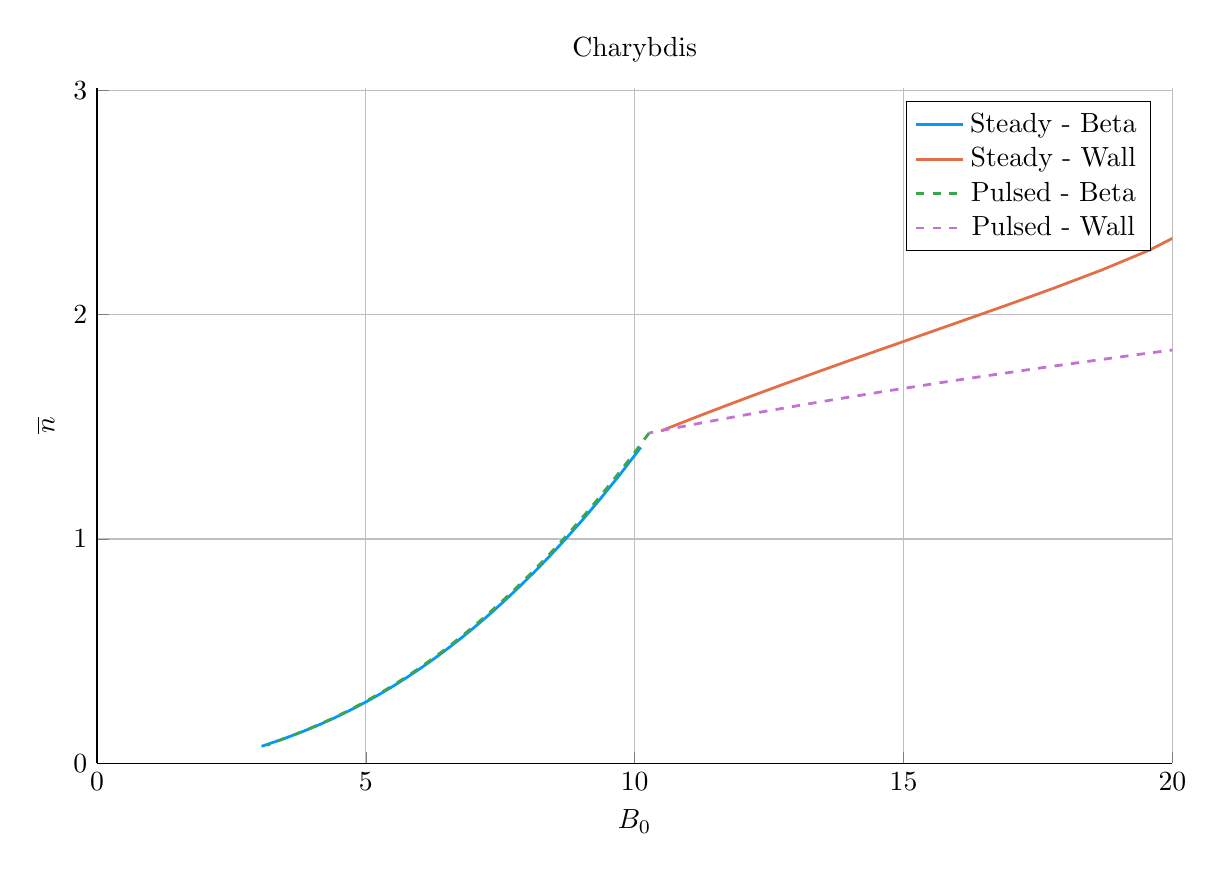
\begin{tikzpicture}[]
\begin{axis}[height = {101.6mm}, ylabel = {$\overline {n}$}, title = {Charybdis}, xmin = {0.0}, xmax = {20.0}, ymax = {3.0106817522827303}, xlabel = {${B}_{0}$}, {unbounded coords=jump, scaled x ticks = false, xticklabel style={rotate = 0}, xmajorgrids = true, xtick = {0.0,5.0,10.0,15.0,20.0}, xticklabels = {0,5,10,15,20}, xtick align = inside, axis lines* = left, scaled y ticks = false, yticklabel style={rotate = 0}, ymajorgrids = true, ytick = {0.0,1.0,2.0,3.0}, yticklabels = {0,1,2,3}, ytick align = inside, axis lines* = left,     xshift = 0.0mm,
    yshift = 0.0mm,
    axis background/.style={fill={rgb,1:red,1.00000000;green,1.00000000;blue,1.00000000}}
, colorbar style={title=}}, ymin = {0.0}, width = {152.4mm}]\addplot+ [color = {rgb,1:red,0.00000000;green,0.60560316;blue,0.97868012},
draw opacity=1.0,
line width=1,
solid,mark = none,
mark size = 2.0,
mark options = {
    color = {rgb,1:red,0.00000000;green,0.00000000;blue,0.00000000}, draw opacity = 1.0,
    fill = {rgb,1:red,0.00000000;green,0.60560316;blue,0.97868012}, fill opacity = 1.0,
    line width = 1,
    rotate = 0,
    solid
}]coordinates {
(10.112818033153026, 1.4080180233503892)
(9.722156888543116, 1.2861639476049844)
(9.357875603858393, 1.1780588306383353)
(9.017653755630063, 1.081850327149118)
(8.6995124437054, 0.9959902151868488)
(8.401566530516865, 0.9191411773935909)
(8.122163706328223, 0.8501712682481828)
(7.859819415455661, 0.7881124422593939)
(7.613196557650265, 0.7321338462491466)
(7.381088038653343, 0.6815199282893232)
(7.162401716104116, 0.6356524139815598)
(6.956147367527331, 0.5939954031881018)
(6.761425371986388, 0.556082996430806)
(6.577416849463348, 0.5215089812627813)
(6.403375044688587, 0.4899182033579257)
(6.2386177769852695, 0.4609993211105009)
(6.0825208065966905, 0.4344787009290932)
(5.934511989185341, 0.4101152563078669)
(5.794066116682695, 0.38769607143982726)
(5.660700347012839, 0.3670326779389849)
(5.533970150598111, 0.3479578783948124)
(5.413465705416883, 0.33032302848637335)
(5.298808685607224, 0.31399570522389186)
(5.189649392059402, 0.2988577008481377)
(5.085664187259174, 0.2848032928860503)
(4.986553195072601, 0.2717377483569661)
(4.892038235455667, 0.259576027456726)
(4.801860966679364, 0.24824165749536697)
(4.7157812114040425, 0.23766575253336641)
(4.633575445956479, 0.2277861580097228)
(4.5550354347559185, 0.21854670285349467)
(4.479966994069385, 0.20989654423645587)
(4.408188871204256, 0.2017895923528845)
(4.33953172691477, 0.19418400448026019)
(4.273837210246432, 0.18704173914418837)
(4.210957116299974, 0.1803281625331897)
(4.15075261849161, 0.17401170042577013)
(4.0930935678432965, 0.16806352983774442)
(4.037857852672517, 0.1624573054000978)
(3.9849308127842145, 0.1571689161601074)
(3.9342047029103653, 0.15217626908008938)
(3.8855782007091695, 0.14745909600508258)
(3.838955955133626, 0.1429987812960845)
(3.7942481714200484, 0.13877820769033083)
(3.7513702293348077, 0.13478161826362128)
(3.710242331663442, 0.13099449263979326)
(3.6707891802306123, 0.12740343582532485)
(3.6329396770109583, 0.12399607824841757)
(3.5966266481325166, 0.1207609857562685)
(3.5617865887889004, 0.11768757847541621)
(3.5283594272686503, 0.11476605757147354)
(3.496288306480746, 0.11198733905884602)
(3.465519381509793, 0.10934299391079556)
(3.4360016318699595, 0.10682519380713147)
(3.4076866872513096, 0.1044266619329971)
(3.380528665662031, 0.10214062830882878)
(3.3544840229690007, 0.09996078918999587)
(3.3295114129297314, 0.09788127012603862)
(3.3055715568879336, 0.09589659231450282)
(3.2826271223788512, 0.09400164192421709)
(3.260642607548369, 0.09219164197560414)
(3.239584247604666, 0.0904621273749388)
(3.2194198921826622, 0.08880892030278893)
(3.2001189373344725, 0.08722811002928488)
(3.181652227422265, 0.08571603269016817)
(3.163991977015565, 0.08426925342486932)
(3.1471116955378684, 0.08288454987069549)
(3.130986116696265, 0.08155889700065513)
(3.115591132350856, 0.08028945318360044)
(3.1009037305081053, 0.07907354735735858)
(3.0869019371473265, 0.07790866721623366)
(3.0735647616124355, 0.07679244832384123)
(3.0608721453218655, 0.07572266407078869)
};
\addlegendentry{Steady - Beta}
\addplot+ [color = {rgb,1:red,0.88887350;green,0.43564919;blue,0.27812294},
draw opacity=1.0,
line width=1,
solid,mark = none,
mark size = 2.0,
mark options = {
    color = {rgb,1:red,0.00000000;green,0.00000000;blue,0.00000000}, draw opacity = 1.0,
    fill = {rgb,1:red,0.88887350;green,0.43564919;blue,0.27812294}, fill opacity = 1.0,
    line width = 1,
    rotate = 0,
    solid
}]coordinates {
(20.758867641064707, 2.4842592400094183)
(20.346250098246923, 2.38278524549101)
(19.57104597888471, 2.287303258882608)
(18.681781921115476, 2.1985633799221938)
(17.775790175980152, 2.116368595866322)
(16.896654716492492, 2.040274511048486)
(16.063927450323227, 1.9697778662839438)
(15.285557510665852, 1.9043839560851952)
(14.563500533069154, 1.8436300461570285)
(13.896568848875791, 1.7870928233184704)
(13.281970890030232, 1.7343892722963155)
(12.716170469467318, 1.685174765875444)
(12.195372283741088, 1.6391400410334225)
(11.715794270833433, 1.5960078401047573)
(11.273815669498969, 1.5555295855068478)
(10.866051794088186, 1.5174822572524134)
(10.489365023931143, 1.481665372051514)
};
\addlegendentry{Steady - Wall}
\addplot+ [color = {rgb,1:red,0.24222430;green,0.64327509;blue,0.30444865},
draw opacity=1.0,
line width=1,
dashed,mark = none,
mark size = 2.0,
mark options = {
    color = {rgb,1:red,0.00000000;green,0.00000000;blue,0.00000000}, draw opacity = 1.0,
    fill = {rgb,1:red,0.24222430;green,0.64327509;blue,0.30444865}, fill opacity = 1.0,
    line width = 1,
    rotate = 0,
    solid
}]coordinates {
(10.26788634689966, 1.4723623744660785)
(9.953967652326213, 1.3711265350676114)
(9.567926244368271, 1.252132124082005)
(9.207974394987358, 1.1465846369072752)
(8.871841888699304, 1.0526756796211467)
(8.557505525932248, 0.9688765933571936)
(8.263156925406376, 0.8938897951240629)
(7.9871752024348766, 0.8266094827857834)
(7.728103682045175, 0.7660897348433404)
(7.484629973620137, 0.7115184848188293)
(7.255568856523303, 0.6621961875986196)
(7.039847526735421, 0.6175182527498871)
(6.836492834698909, 0.5769605172018885)
(6.644620209081183, 0.5400671818578971)
(6.463424013335149, 0.5064407547071686)
(6.2921691243175495, 0.4757336350189907)
(6.13018355681404, 0.4476410453280237)
(5.97685198655569, 0.42189507479572563)
(5.831610044919842, 0.3982596421732652)
(5.693939286027163, 0.3765262234359318)
(5.563362729090489, 0.35651021595970495)
(5.439440906144732, 0.33804783586593384)
(5.321768347746793, 0.3209934625186893)
(5.209970453003084, 0.3052173596602331)
(5.103700692769835, 0.2906037142188434)
(5.002638109938164, 0.2770489446480202)
(4.906485077678376, 0.26446023780008615)
(4.814965286571576, 0.252754280569387)
(4.727821933804548, 0.2418561578126615)
(4.644816091323922, 0.23169839260513847)
(4.565725232806084, 0.22222010863842148)
(4.490341901840154, 0.21336629768120086)
(4.418472505906755, 0.20508717762073375)
(4.349936222622964, 0.1973376287742364)
(4.284564006352339, 0.19007669797920612)
(4.222197684694192, 0.18326716150163008)
(4.162689135592264, 0.17687513909003888)
(4.105899536872315, 0.17086975259243936)
(4.051698680949713, 0.16522282347532805)
(3.9999643482627323, 0.15990860436675383)
(3.9505817337017928, 0.15490354041139245)
(3.903442920928527, 0.15018605679322225)
(3.858446400032002, 0.14573636926674546)
(3.8154966244515616, 0.14153631495294655)
(3.7745036035252744, 0.13756920101269954)
(3.7353825273991994, 0.13381966911666454)
(3.6980534213689746, 0.13027357389473523)
(3.6624408270205375, 0.12691787377578978)
(3.62847350780097, 0.1237405328254604)
(3.5960841768845415, 0.12073043236018116)
(3.565209245407392, 0.11787729126371532)
(3.5357885893311605, 0.11517159406103483)
(3.5077653333614305, 0.11260452591630596)
(3.4810856504959875, 0.11016791381940663)
(3.4556985759109375, 0.1078541733106241)
(3.4315558340122845, 0.10565626016776815)
(3.408611677587535, 0.10356762654523782)
(3.3868227380888998, 0.10158218111191525)
(3.36614788616562, 0.09969425278506897)
(3.3465481016421226, 0.09789855770179177)
(3.327986352208224, 0.09619016910847078)
(3.3104274769652595, 0.09456448972221645)
(3.2938380965241474, 0.09301722743690491)
(3.278186482171801, 0.09154437076423085)
(3.263442495132517, 0.09014216944229511)
(3.2495774839156075, 0.0888071143925177)
(3.236564206241785, 0.0875359202427047)
(3.224376752844934, 0.08632550914162683)
(3.212990475972638, 0.08517299589362785)
(3.2023819222517877, 0.08407567429398183)
(3.192528769611062, 0.08303100455746225)
(3.1834097679780142, 0.08203660174317265)
(3.1750046834890777, 0.0810902250880436)
(3.1672942459724482, 0.08018976816986731)
};
\addlegendentry{Pulsed - Beta}
\addplot+ [color = {rgb,1:red,0.76444018;green,0.44411178;blue,0.82429754},
draw opacity=1.0,
line width=1,
dashed,mark = none,
mark size = 2.0,
mark options = {
    color = {rgb,1:red,0.00000000;green,0.00000000;blue,0.00000000}, draw opacity = 1.0,
    fill = {rgb,1:red,0.76444018;green,0.44411178;blue,0.82429754}, fill opacity = 1.0,
    line width = 1,
    rotate = 0,
    solid
}]coordinates {
(48.990476413653056, 2.5089014602356086)
(42.83950920694117, 2.3949108855368064)
(37.687790427214495, 2.290982472948034)
(33.33937742845888, 2.195911174285586)
(29.64296398154308, 2.1086702915756774)
(26.48039367255613, 2.0283805298641298)
(23.758442882319894, 1.9542851453933179)
(21.402860298405816, 1.8857298558917068)
(19.353987387634486, 1.8221464985140954)
(17.563502020363714, 1.763039657371641)
(15.991970371213752, 1.7079756596238989)
(14.606987499719377, 1.6565734722259482)
(13.381751501116137, 1.6084971330058802)
(12.293960329570087, 1.5634494271559283)
(11.32495111804522, 1.521166580022558)
(10.459023415380802, 1.4814137834199246)
(10.26788634689966, 1.4723623744660785)
};
\addlegendentry{Pulsed - Wall}
\end{axis}

\end{tikzpicture}

    \end{adjustbox}
        \caption{Charybdis}
    \end{subfigure}
    \hfill
    \begin{subfigure}[t]{0.45\textwidth}
        \centering
    \begin{adjustbox}{width=\textwidth}
      \Large
      \begin{tikzpicture}[]
\begin{axis}[height = {101.6mm}, ylabel = {$\overline {n}$}, title = {Proteus}, xmin = {0.0}, xmax = {20.0}, ymax = {1.6027133106922544}, xlabel = {${B}_{0}$}, {unbounded coords=jump, scaled x ticks = false, xticklabel style={rotate = 0}, xmajorgrids = true, xtick = {0.0,5.0,10.0,15.0,20.0}, xticklabels = {0,5,10,15,20}, xtick align = inside, axis lines* = left, scaled y ticks = false, yticklabel style={rotate = 0}, ymajorgrids = true, ytick = {0.0,0.5,1.0,1.5}, yticklabels = {0.0,0.5,1.0,1.5}, ytick align = inside, axis lines* = left,     xshift = 0.0mm,
    yshift = 0.0mm,
    axis background/.style={fill={rgb,1:red,1.00000000;green,1.00000000;blue,1.00000000}}
, colorbar style={title=}}, ymin = {0.0}, width = {152.4mm}]\addplot+ [color = {rgb,1:red,0.00000000;green,0.60560316;blue,0.97868012},
draw opacity=1.0,
line width=1,
solid,mark = none,
mark size = 2.0,
mark options = {
    color = {rgb,1:red,0.00000000;green,0.00000000;blue,0.00000000}, draw opacity = 1.0,
    fill = {rgb,1:red,0.00000000;green,0.60560316;blue,0.97868012}, fill opacity = 1.0,
    line width = 1,
    rotate = 0,
    solid
}]coordinates {
(4.658732060637907, 0.43980673694046557)
(4.211109766361548, 0.4555835431053639)
(3.9293920326356777, 0.4746023245444401)
(3.7651903683456465, 0.4969874735748488)
(3.6776039543745567, 0.5220861763665989)
(3.6402437753208394, 0.5492525801629207)
(3.6366994671255806, 0.5779851566743729)
(3.656621534643579, 0.6079145499927882)
(3.693300156736026, 0.6387689849987517)
(3.7422515017241134, 0.6703447016435368)
(3.865532743079537, 0.7350646189649392)
(3.936096932264377, 0.7679824016591842)
(4.010907188015084, 0.801152382186179)
(4.089072356933184, 0.8345005323193241)
(4.169903401491354, 0.8679614824642194)
(4.252857906625248, 0.9014764199291089)
(4.337501757261618, 0.9349916267666121)
(4.42348218754058, 0.9684574586630934)
(4.5983381267510195, 1.0350587268600935)
(4.686766232902671, 1.0681098483996954)
(4.775618142770625, 1.1009423941840293)
(4.864743502376605, 1.133519904373093)
(4.927312314219091, 1.1561859575921225)
};
\addlegendentry{Pulsed - Kink}
\addplot+ [color = {rgb,1:red,0.88887350;green,0.43564919;blue,0.27812294},
draw opacity=1.0,
line width=1,
solid,mark = none,
mark size = 2.0,
mark options = {
    color = {rgb,1:red,0.00000000;green,0.00000000;blue,0.00000000}, draw opacity = 1.0,
    fill = {rgb,1:red,0.88887350;green,0.43564919;blue,0.27812294}, fill opacity = 1.0,
    line width = 1,
    rotate = 0,
    solid
}]coordinates {
(4.927312314219091, 1.1561859575921225)
(4.984545814413324, 1.1643302061382435)
(5.17452482724068, 1.1909307182551652)
(5.362091669637646, 1.2165101695399059)
(5.54700293215903, 1.2410246741167772)
(5.729042482638278, 1.2644405260926448)
(5.908022832274664, 1.2867341960657983)
(6.083785777786694, 1.3078920833503354)
(6.256202341425288, 1.3279100448430345)
(6.324169421042356, 1.3355944255768788)
};
\addlegendentry{Pulsed - Beta}
\addplot+ [color = {rgb,1:red,0.24222430;green,0.64327509;blue,0.30444865},
draw opacity=1.0,
line width=1,
solid,mark = none,
mark size = 2.0,
mark options = {
    color = {rgb,1:red,0.00000000;green,0.00000000;blue,0.00000000}, draw opacity = 1.0,
    fill = {rgb,1:red,0.24222430;green,0.64327509;blue,0.30444865}, fill opacity = 1.0,
    line width = 1,
    rotate = 0,
    solid
}]coordinates {
(6.324169421042356, 1.3355944255768788)
(6.727338549778396, 1.3196535263642608)
(7.320469048424473, 1.293132444381878)
(7.835746509376305, 1.267102506645195)
(8.290245520072391, 1.241842432239768)
(8.696162676727877, 1.2174861553396652)
(9.0624397222742, 1.1940889283561482)
(9.395798186463841, 1.1716618573954198)
(9.701405747258567, 1.1501909086306326)
(10.244760202900984, 1.1099965067246496)
(10.930275827723788, 1.0559880902978025)
(11.131878682735255, 1.03949661084059)
(11.50278450645086, 1.0085444915557933)
(11.83715172742864, 0.9800605714948162)
(11.992609772603878, 0.9666615553001195)
(12.141110720831467, 0.953784249057476)
};
\addlegendentry{Pulsed - Wall}
\end{axis}

\end{tikzpicture}

    \end{adjustbox}
        \caption{Proteus}
    \end{subfigure}
    \hfill \hfill ~\\ ~\\ ~\\ ~\\
    \hfill
    \begin{subfigure}[t]{0.45\textwidth}
        \centering
    \begin{adjustbox}{width=\textwidth}
      \Large
      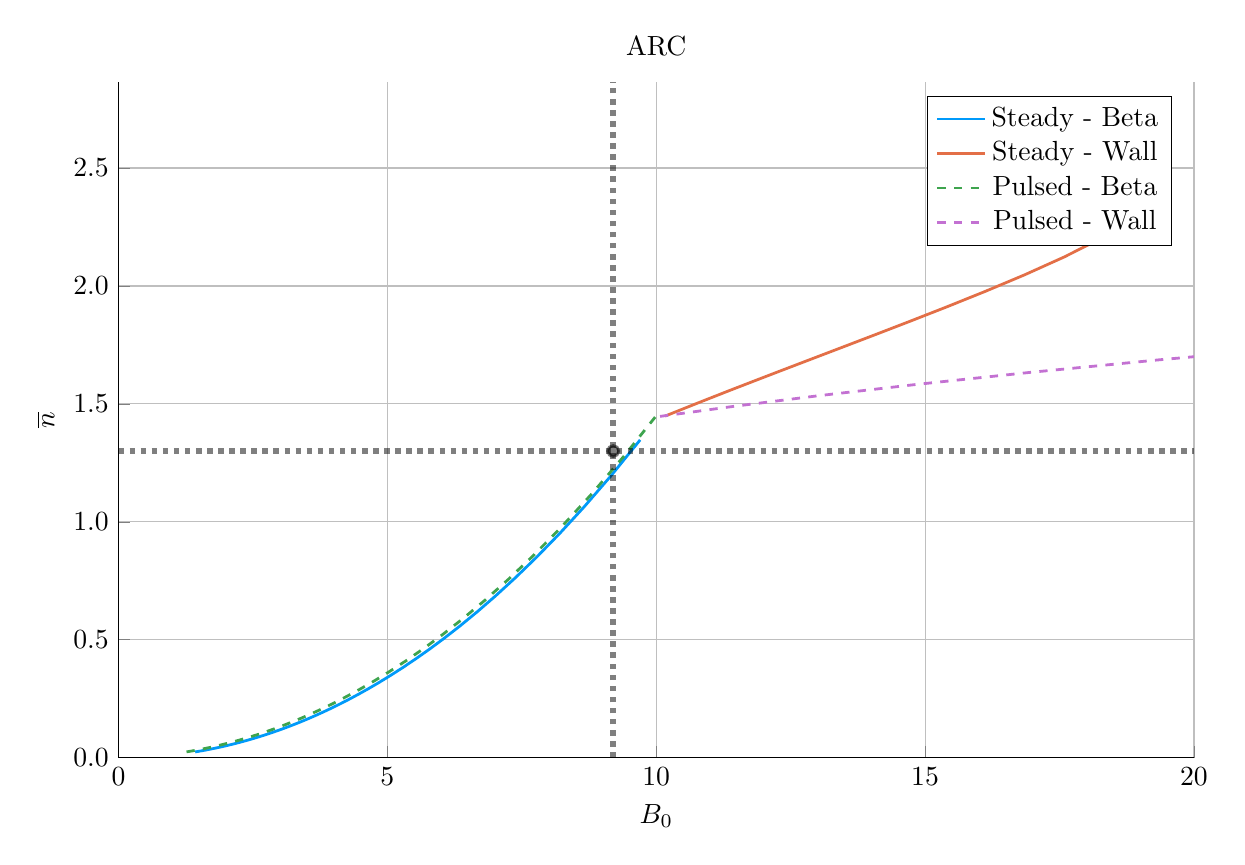
\begin{tikzpicture}[]
\begin{axis}[height = {101.6mm}, ylabel = {$\overline {n}$}, title = {ARC}, xmin = {0.0}, xmax = {20.0}, ymax = {2.863990591552692}, xlabel = {${B}_{0}$}, {unbounded coords=jump, scaled x ticks = false, xticklabel style={rotate = 0}, xmajorgrids = true, xtick = {0.0,5.0,10.0,15.0,20.0}, xticklabels = {0,5,10,15,20}, xtick align = inside, axis lines* = left, scaled y ticks = false, yticklabel style={rotate = 0}, ymajorgrids = true, ytick = {0.0,0.5,1.0,1.5,2.0,2.5}, yticklabels = {0.0,0.5,1.0,1.5,2.0,2.5}, ytick align = inside, axis lines* = left,     xshift = 0.0mm,
    yshift = 0.0mm,
    axis background/.style={fill={rgb,1:red,1.00000000;green,1.00000000;blue,1.00000000}}
, colorbar style={title=}}, ymin = {0.0}, width = {152.4mm}]\addplot+ [color = {rgb,1:red,0.00000000;green,0.60560316;blue,0.97868012},
draw opacity=1.0,
line width=1,
solid,mark = none,
mark size = 2.0,
mark options = {
    color = {rgb,1:red,0.00000000;green,0.00000000;blue,0.00000000}, draw opacity = 1.0,
    fill = {rgb,1:red,0.00000000;green,0.60560316;blue,0.97868012}, fill opacity = 1.0,
    line width = 1,
    rotate = 0,
    solid
}]coordinates {
(9.701206080853105, 1.3473195408198368)
(9.162315904693079, 1.1960181602975513)
(8.664301107137337, 1.0646278606603214)
(8.203576462497304, 0.9502233495133008)
(7.776718537485166, 0.8503139853090188)
(7.380720231870917, 0.7628227562648452)
(7.012886014999712, 0.6860021637884806)
(6.670795005901889, 0.6183771311663153)
(6.352268997292712, 0.558698610226677)
(6.055344682097163, 0.5059057339549363)
(5.778249464564785, 0.4590948250110799)
(5.519380338856715, 0.41749392677128644)
(5.2772854007125325, 0.3804418002600398)
(5.050647625972996, 0.3473705460934129)
(4.838270606140816, 0.3177911795286596)
(4.639065978019038, 0.2912816196341205)
(4.4520423235376105, 0.26747665859063235)
(4.276295348572609, 0.2460595604126924)
(4.110999177018484, 0.22675500468553664)
(3.9553986195015125, 0.20932314390860127)
(3.8088022956698633, 0.19355458554339033)
(3.6705765055641186, 0.17926614407860172)
(3.54013975965751, 0.1662972360582311)
(3.4169578891619192, 0.1545068134081091)
(3.30053966845824, 0.1437707485950006)
(3.1904328903033052, 0.13397959998952993)
(3.086220842019516, 0.12503669793657493)
(2.9875191373772063, 0.11685650198571602)
(2.8939728644914635, 0.1093631879154991)
(2.8052540149097247, 0.10248942993093182)
(2.7210591632720242, 0.09617534899013032)
(2.6411073705789065, 0.09036760283780103)
(2.565138287279709, 0.0850185971631545)
(2.492910435164382, 0.08008580049787432)
(2.4241996494611984, 0.07553114813940931)
(2.3587976646588236, 0.07132052261851271)
(2.296510829425685, 0.0674233001029537)
(2.237158937627476, 0.06381195370335846)
(2.180574163874242, 0.0604617059726188)
(2.126600093288366, 0.057350224008889575)
(2.075090836295778, 0.05445735151799167)
(2.0259102202234582, 0.051764872992355326)
(1.978931050353818, 0.04925630584382654)
(1.9340344338545452, 0.046916716906113216)
(1.8911091606836798, 0.04473256021550835)
(1.8500511361739687, 0.042691533399160944)
(1.8107628605384507, 0.04078245035985612)
(1.773152951016952, 0.03899512825429317)
(1.7371357028100902, 0.03732028702616347)
(1.7026306853269466, 0.03574945998241189)
(1.6695623706125668, 0.03427491409656386)
(1.6378597911249178, 0.03288957889151024)
(1.607456224302725, 0.03158698289964531)
(1.5782889016090462, 0.030361196824073462)
(1.5502987399539199, 0.02920678263355747)
(1.5234300935954943, 0.028118747918386335)
(1.4976305247952577, 0.02709250491641066)
(1.4728505916614916, 0.026123833689876915)
(1.4490436517578602, 0.02520884899586455)
(1.4261656801829077, 0.024343970447355107)
};
\addlegendentry{Steady - Beta}
\addplot+ [color = {rgb,1:red,0.88887350;green,0.43564919;blue,0.27812294},
draw opacity=1.0,
line width=1,
solid,mark = none,
mark size = 2.0,
mark options = {
    color = {rgb,1:red,0.00000000;green,0.00000000;blue,0.00000000}, draw opacity = 1.0,
    fill = {rgb,1:red,0.88887350;green,0.43564919;blue,0.27812294}, fill opacity = 1.0,
    line width = 1,
    rotate = 0,
    solid
}]coordinates {
(19.394007482712425, 2.38665882629391)
(18.932196567189358, 2.2924313547124413)
(18.296989378345195, 2.2045266222525584)
(17.587029315408756, 2.12281365923743)
(16.847882407994106, 2.046875568311427)
(16.111374502564406, 1.9762927537752475)
(15.396027314547156, 1.9106370808732966)
(14.710952688793137, 1.8494873568146586)
(14.06168447794857, 1.7924599120221316)
(13.450465418483889, 1.7392009020858583)
(12.877644538645335, 1.6893881894372746)
(12.342394470642008, 1.6427297299399706)
(11.843182246608265, 1.5989613537444864)
(11.376441269625893, 1.5578311981599224)
(10.944966372727551, 1.5191630469025923)
(10.541663878705513, 1.4827225505089883)
(10.165908182236457, 1.4483456743918615)
};
\addlegendentry{Steady - Wall}
\addplot+ [color = {rgb,1:red,0.24222430;green,0.64327509;blue,0.30444865},
draw opacity=1.0,
line width=1,
dashed,mark = none,
mark size = 2.0,
mark options = {
    color = {rgb,1:red,0.00000000;green,0.00000000;blue,0.00000000}, draw opacity = 1.0,
    fill = {rgb,1:red,0.24222430;green,0.64327509;blue,0.30444865}, fill opacity = 1.0,
    line width = 1,
    rotate = 0,
    solid
}]coordinates {
(9.980483622051658, 1.4439851501001137)
(9.392786903460065, 1.2762634218469477)
(8.79273598103983, 1.1162231297529333)
(8.23820290909994, 0.9782947350570418)
(7.725182218401588, 0.859142163942709)
(7.250078106370205, 0.7559761709746792)
(6.80965553466646, 0.666457312509999)
(6.400998063035608, 0.5886174855235811)
(6.0214713600430425, 0.5207962164260873)
(5.668691517461799, 0.4615887229256594)
(5.340497445229901, 0.4098034143236215)
(5.034926745580058, 0.36442699044958116)
(4.750194564008521, 0.3245956826357914)
(4.484674995755211, 0.2895714783883623)
(4.236884692979903, 0.25872240468547436)
(4.00546837264544, 0.23150612812536642)
(3.7891859704718387, 0.2074562748071761)
(3.5869012239550364, 0.18617098748314467)
(3.3975714987448393, 0.16730332876490603)
(3.2202386987489797, 0.1505532120625826)
(3.0540211220494466, 0.13566060039019867)
(2.8981061427709687, 0.1223997602125144)
(2.7517436139566023, 0.11057439549352384)
(2.6142398986781377, 0.10001351787782128)
(2.4849524463010138, 0.09056793393747618)
(2.363284838174807, 0.08210725078641655)
(2.248682232019848, 0.07451731799864314)
(2.140627136740878, 0.06769803737486514)
(2.038635448877246, 0.061561483243502586)
(1.9422526775794744, 0.05603028509466519)
(1.8510502754751532, 0.051036231767032654)
(1.7646219756564088, 0.04651906238493242)
(1.6825800061969869, 0.042425413935321434)
(1.6045510059627948, 0.03870789883811779)
(1.53017138625397, 0.035324288011568686)
(1.4590817483192686, 0.03223677544299094)
(1.3909197311384796, 0.02941129837282704)
(1.3253102336217724, 0.026816881184046584)
(1.261851128383913, 0.024424957151690567)
(1.20009089049112, 0.022208591361068685)
(1.1394908096975784, 0.02014145733294951)
};
\addlegendentry{Pulsed - Beta}
\addplot+ [color = {rgb,1:red,0.76444018;green,0.44411178;blue,0.82429754},
draw opacity=1.0,
line width=1,
dashed,mark = none,
mark size = 2.0,
mark options = {
    color = {rgb,1:red,0.00000000;green,0.00000000;blue,0.00000000}, draw opacity = 1.0,
    fill = {rgb,1:red,0.76444018;green,0.44411178;blue,0.82429754}, fill opacity = 1.0,
    line width = 1,
    rotate = 0,
    solid
}]coordinates {
(29.27715761652869, 1.8712109568011082)
(25.4410619834368, 1.8054178931700802)
(22.158819835998365, 1.7440059619090504)
(19.342453256965573, 1.6865690155045403)
(16.919364280634177, 1.6327482182979707)
(14.829378672669455, 1.582225517657922)
(13.022412368922526, 1.5347181466466893)
(11.456617692058645, 1.4899739758924049)
(10.096901921254785, 1.447767567796814)
(9.980483622051658, 1.4439851501001137)
};
\addlegendentry{Pulsed - Wall}
\addplot+ [color = {rgb,1:red,0.00000000;green,0.00000000;blue,0.00000000},
draw opacity=0.5,
line width=2,
dotted,mark = none,
mark size = 2.0,
mark options = {
    color = {rgb,1:red,0.00000000;green,0.00000000;blue,0.00000000}, draw opacity = 0.5,
    fill = {rgb,1:red,0.00000000;green,0.00000000;blue,0.00000000}, fill opacity = 0.5,
    line width = 1,
    rotate = 0,
    solid
},forget plot]coordinates {
(0.0, 1.3)
(20.0, 1.3)
};
\addplot+ [color = {rgb,1:red,0.00000000;green,0.00000000;blue,0.00000000},
draw opacity=0.5,
line width=2,
dotted,mark = none,
mark size = 2.0,
mark options = {
    color = {rgb,1:red,0.00000000;green,0.00000000;blue,0.00000000}, draw opacity = 0.5,
    fill = {rgb,1:red,0.00000000;green,0.00000000;blue,0.00000000}, fill opacity = 0.5,
    line width = 1,
    rotate = 0,
    solid
},forget plot]coordinates {
(9.2, 0.0)
(9.2, 2.863990591552692)
};
\addplot+[draw=none, color = {rgb,1:red,0.00000000;green,0.00000000;blue,0.00000000},
draw opacity=0.5,
line width=0,
solid,mark = *,
mark size = 2.0,
mark options = {
    color = {rgb,1:red,0.00000000;green,0.00000000;blue,0.00000000}, draw opacity = 0.5,
    fill = {rgb,1:red,0.00000000;green,0.00000000;blue,0.00000000}, fill opacity = 0.5,
    line width = 1,
    rotate = 0,
    solid
},forget plot] coordinates {
(9.2, 1.3)
};
\end{axis}

\end{tikzpicture}

    \end{adjustbox}
        \caption{ARC}
    \end{subfigure}
    \hfill
    \begin{subfigure}[t]{0.45\textwidth}
        \centering
    \begin{adjustbox}{width=\textwidth}
      \Large
      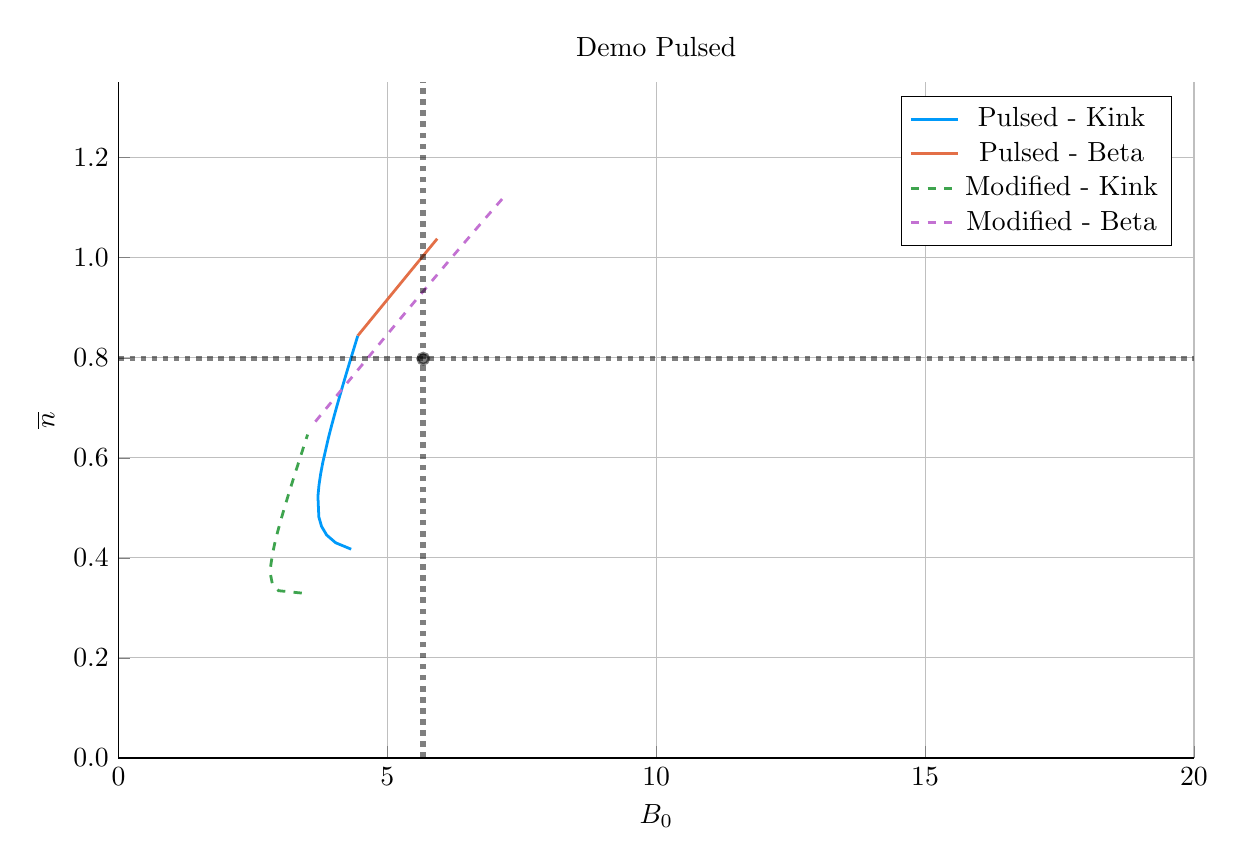
\begin{tikzpicture}[]
\begin{axis}[height = {101.6mm}, ylabel = {$\overline {n}$}, title = {Demo Pulsed}, xmin = {0.0}, xmax = {20.0}, ymax = {1.3503983107514914}, xlabel = {${B}_{0}$}, {unbounded coords=jump, scaled x ticks = false, xticklabel style={rotate = 0}, xmajorgrids = true, xtick = {0.0,5.0,10.0,15.0,20.0}, xticklabels = {0,5,10,15,20}, xtick align = inside, axis lines* = left, scaled y ticks = false, yticklabel style={rotate = 0}, ymajorgrids = true, ytick = {0.0,0.2,0.4,0.6000000000000001,0.8,1.0,1.2000000000000002}, yticklabels = {0.0,0.2,0.4,0.6,0.8,1.0,1.2}, ytick align = inside, axis lines* = left,     xshift = 0.0mm,
    yshift = 0.0mm,
    axis background/.style={fill={rgb,1:red,1.00000000;green,1.00000000;blue,1.00000000}}
, colorbar style={title=}}, ymin = {0.0}, width = {152.4mm}]\addplot+ [color = {rgb,1:red,0.00000000;green,0.60560316;blue,0.97868012},
draw opacity=1.0,
line width=1,
solid,mark = none,
mark size = 2.0,
mark options = {
    color = {rgb,1:red,0.00000000;green,0.00000000;blue,0.00000000}, draw opacity = 1.0,
    fill = {rgb,1:red,0.00000000;green,0.60560316;blue,0.97868012}, fill opacity = 1.0,
    line width = 1,
    rotate = 0,
    solid
}]coordinates {
(4.327031075670194, 0.41734809072093004)
(4.038214026054326, 0.43024493827565713)
(3.8713719163129245, 0.4456891288507263)
(3.7758613845615545, 0.4630422682794791)
(3.7257856761317214, 0.48187273793982344)
(3.7090473695925437, 0.5228878532025801)
(3.727711597554826, 0.5447265162402501)
(3.7586131667481433, 0.5672993399625227)
(3.799052518631718, 0.5905272108832595)
(3.901290136389271, 0.6387170091650386)
(3.960577465316514, 0.663591827304985)
(4.0241209645210345, 0.6889413712914579)
(4.0912717805663785, 0.7147383569784123)
(4.161514602943343, 0.7409591895293305)
(4.2344343960723005, 0.7675830424708951)
(4.309692554546368, 0.7945911767140547)
(4.450417240491067, 0.8442005157357652)
};
\addlegendentry{Pulsed - Kink}
\addplot+ [color = {rgb,1:red,0.88887350;green,0.43564919;blue,0.27812294},
draw opacity=1.0,
line width=1,
solid,mark = none,
mark size = 2.0,
mark options = {
    color = {rgb,1:red,0.00000000;green,0.00000000;blue,0.00000000}, draw opacity = 1.0,
    fill = {rgb,1:red,0.88887350;green,0.43564919;blue,0.27812294}, fill opacity = 1.0,
    line width = 1,
    rotate = 0,
    solid
}]coordinates {
(4.450417240491067, 0.8442005157357652)
(4.490148631384312, 0.8494249638279073)
(4.692490181445514, 0.8760451902718939)
(4.8960344619053355, 0.9028334122917245)
(5.100651132702229, 0.9297551501591124)
(5.306202822090688, 0.9567754052429361)
(5.512545696627038, 0.9838586056021301)
(5.719530043226767, 1.010968600058316)
(5.927000883375481, 1.0380686957167213)
};
\addlegendentry{Pulsed - Beta}
\addplot+ [color = {rgb,1:red,0.24222430;green,0.64327509;blue,0.30444865},
draw opacity=1.0,
line width=1,
dashed,mark = none,
mark size = 2.0,
mark options = {
    color = {rgb,1:red,0.00000000;green,0.00000000;blue,0.00000000}, draw opacity = 1.0,
    fill = {rgb,1:red,0.24222430;green,0.64327509;blue,0.30444865}, fill opacity = 1.0,
    line width = 1,
    rotate = 0,
    solid
}]coordinates {
(3.4087424183072135, 0.32962263686290805)
(2.977074181068944, 0.3344062300712191)
(2.8592500074202523, 0.34896612080740375)
(2.827199220063259, 0.3667528822318307)
(2.8339789008667826, 0.3862562920813225)
(2.862412302880871, 0.4068948911211116)
(2.9044598258085443, 0.4283880296875811)
(2.95577893007882, 0.45058078235145627)
(3.0137895352525907, 0.4733793591195171)
(3.076849710218805, 0.49672284599169997)
(3.1438583711612704, 0.5205693124594925)
(3.214045733980633, 0.5448883758700154)
(3.2868548955983727, 0.5696569551809978)
(3.361871149981842, 0.5948567190533759)
(3.4387778750377818, 0.6204724875804614)
(3.5173279629378453, 0.6464911965506945)
};
\addlegendentry{Modified - Kink}
\addplot+ [color = {rgb,1:red,0.76444018;green,0.44411178;blue,0.82429754},
draw opacity=1.0,
line width=1,
dashed,mark = none,
mark size = 2.0,
mark options = {
    color = {rgb,1:red,0.00000000;green,0.00000000;blue,0.00000000}, draw opacity = 1.0,
    fill = {rgb,1:red,0.76444018;green,0.44411178;blue,0.82429754}, fill opacity = 1.0,
    line width = 1,
    rotate = 0,
    solid
}]coordinates {
(3.6607028750648505, 0.6723555509280342)
(3.8574448036470477, 0.6980917571451202)
(4.056375867871351, 0.7240979215847156)
(4.257366397480293, 0.7503469025010585)
(4.460279103534801, 0.7768105417816143)
(4.664969389370631, 0.8034595075704105)
(4.871285596007394, 0.8302631937638083)
(5.07906923307514, 0.8571896679457696)
(5.288155233306219, 0.8842056626199803)
(5.498372259673351, 0.911276606653906)
(5.709543087166185, 0.9383666950425207)
(5.921485076209294, 0.9654389956885661)
(6.134010749367255, 0.9924555919974454)
(6.346928478632384, 1.0193777598402507)
(6.560043285872518, 1.0461661769082227)
(6.773157754368795, 1.0727811617497953)
(6.986073044284746, 1.09918293890144)
(7.198590001107076, 1.1253319256262428)
};
\addlegendentry{Modified - Beta}
\addplot+ [color = {rgb,1:red,0.00000000;green,0.00000000;blue,0.00000000},
draw opacity=0.5,
line width=2,
dotted,mark = none,
mark size = 2.0,
mark options = {
    color = {rgb,1:red,0.00000000;green,0.00000000;blue,0.00000000}, draw opacity = 0.5,
    fill = {rgb,1:red,0.00000000;green,0.00000000;blue,0.00000000}, fill opacity = 0.5,
    line width = 1,
    rotate = 0,
    solid
},forget plot]coordinates {
(0.0, 0.7983)
(20.0, 0.7983)
};
\addplot+ [color = {rgb,1:red,0.00000000;green,0.00000000;blue,0.00000000},
draw opacity=0.5,
line width=2,
dotted,mark = none,
mark size = 2.0,
mark options = {
    color = {rgb,1:red,0.00000000;green,0.00000000;blue,0.00000000}, draw opacity = 0.5,
    fill = {rgb,1:red,0.00000000;green,0.00000000;blue,0.00000000}, fill opacity = 0.5,
    line width = 1,
    rotate = 0,
    solid
},forget plot]coordinates {
(5.667, 0.0)
(5.667, 1.3503983107514914)
};
\addplot+[draw=none, color = {rgb,1:red,0.00000000;green,0.00000000;blue,0.00000000},
draw opacity=0.5,
line width=0,
solid,mark = *,
mark size = 2.0,
mark options = {
    color = {rgb,1:red,0.00000000;green,0.00000000;blue,0.00000000}, draw opacity = 0.5,
    fill = {rgb,1:red,0.00000000;green,0.00000000;blue,0.00000000}, fill opacity = 0.5,
    line width = 1,
    rotate = 0,
    solid
},forget plot] coordinates {
(5.667, 0.7983)
};
\end{axis}

\end{tikzpicture}

    \end{adjustbox}
        \caption{DEMO Pulsed}
    \end{subfigure}
    \hfill \hfill ~\\ ~\\ ~\\ ~\\
    \hfill
    \begin{subfigure}[t]{0.45\textwidth}
        \centering
    \begin{adjustbox}{width=\textwidth}
      \Large
      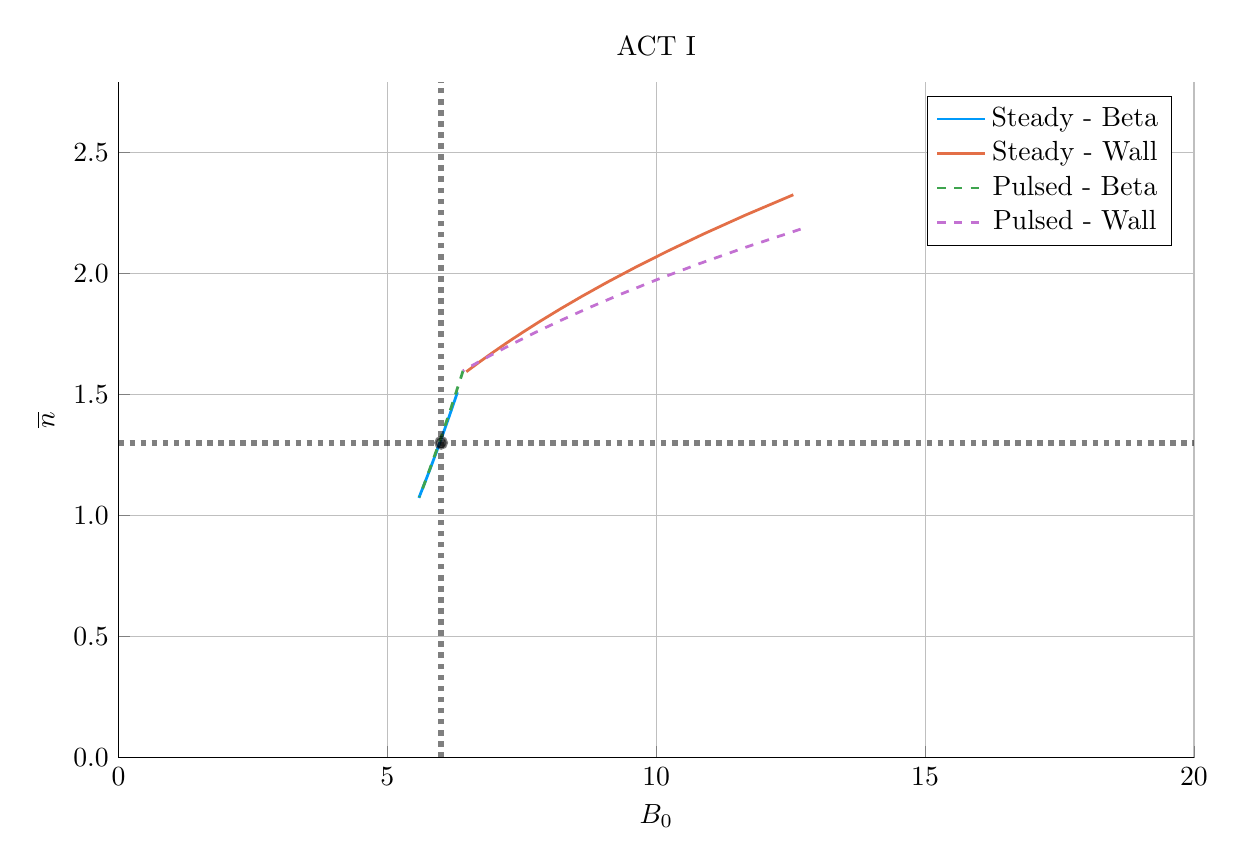
\begin{tikzpicture}[]
\begin{axis}[height = {101.6mm}, ylabel = {$\overline {n}$}, title = {ACT I}, xmin = {0.0}, xmax = {20.0}, ymax = {2.789182184123441}, xlabel = {${B}_{0}$}, {unbounded coords=jump, scaled x ticks = false, xticklabel style={rotate = 0}, xmajorgrids = true, xtick = {0.0,5.0,10.0,15.0,20.0}, xticklabels = {0,5,10,15,20}, xtick align = inside, axis lines* = left, scaled y ticks = false, yticklabel style={rotate = 0}, ymajorgrids = true, ytick = {0.0,0.5,1.0,1.5,2.0,2.5}, yticklabels = {0.0,0.5,1.0,1.5,2.0,2.5}, ytick align = inside, axis lines* = left,     xshift = 0.0mm,
    yshift = 0.0mm,
    axis background/.style={fill={rgb,1:red,1.00000000;green,1.00000000;blue,1.00000000}}
, colorbar style={title=}}, ymin = {0.0}, width = {152.4mm}]\addplot+ [color = {rgb,1:red,0.00000000;green,0.60560316;blue,0.97868012},
draw opacity=1.0,
line width=1,
solid,mark = none,
mark size = 2.0,
mark options = {
    color = {rgb,1:red,0.00000000;green,0.00000000;blue,0.00000000}, draw opacity = 1.0,
    fill = {rgb,1:red,0.00000000;green,0.60560316;blue,0.97868012}, fill opacity = 1.0,
    line width = 1,
    rotate = 0,
    solid
}]coordinates {
(6.30336807958207, 1.508799726687277)
(6.162193069273141, 1.416990530835724)
(6.030717178404645, 1.334162814934454)
(5.908065509576601, 1.259196071868462)
(5.793464904530972, 1.1911374719468464)
(5.686229631357383, 1.1291729026430304)
(5.585749511271037, 1.072603667815424)
};
\addlegendentry{Steady - Beta}
\addplot+ [color = {rgb,1:red,0.88887350;green,0.43564919;blue,0.27812294},
draw opacity=1.0,
line width=1,
solid,mark = none,
mark size = 2.0,
mark options = {
    color = {rgb,1:red,0.00000000;green,0.00000000;blue,0.00000000}, draw opacity = 1.0,
    fill = {rgb,1:red,0.88887350;green,0.43564919;blue,0.27812294}, fill opacity = 1.0,
    line width = 1,
    rotate = 0,
    solid
}]coordinates {
(12.549536249695134, 2.3243184867695343)
(11.658754653696462, 2.240255685209082)
(10.883719833507003, 2.162701818439558)
(10.206258129789394, 2.0909838859446395)
(9.611335769312953, 2.024510647992687)
(9.086446934250878, 1.9627612472481373)
(8.62129895070743, 1.9052777489669976)
(8.207216040989662, 1.8516543635202913)
(7.837119555085499, 1.8015342424723413)
(7.505047858717157, 1.7546005605569122)
(7.20604322925957, 1.7105725385641783)
(6.935884710193303, 1.6691995856432549)
(6.691016583192173, 1.6302582914995123)
(6.468415485086983, 1.593548773199814)
};
\addlegendentry{Steady - Wall}
\addplot+ [color = {rgb,1:red,0.24222430;green,0.64327509;blue,0.30444865},
draw opacity=1.0,
line width=1,
dashed,mark = none,
mark size = 2.0,
mark options = {
    color = {rgb,1:red,0.00000000;green,0.00000000;blue,0.00000000}, draw opacity = 1.0,
    fill = {rgb,1:red,0.24222430;green,0.64327509;blue,0.30444865}, fill opacity = 1.0,
    line width = 1,
    rotate = 0,
    solid
}]coordinates {
(6.408263337806559, 1.5977657032448143)
(6.408263337806564, 1.5977657032448165)
(6.385466513301022, 1.581825496311201)
(6.245492502072912, 1.4856415470557256)
(6.116010320461132, 1.3992276392060343)
(5.9960421481916395, 1.3213241728992242)
(5.884727159112828, 1.250866007536012)
(5.781304768121868, 1.1869479236448208)
(5.685100648450046, 1.1287969651625331)
(5.595515000321003, 1.0757501511002947)
};
\addlegendentry{Pulsed - Beta}
\addplot+ [color = {rgb,1:red,0.76444018;green,0.44411178;blue,0.82429754},
draw opacity=1.0,
line width=1,
dashed,mark = none,
mark size = 2.0,
mark options = {
    color = {rgb,1:red,0.00000000;green,0.00000000;blue,0.00000000}, draw opacity = 1.0,
    fill = {rgb,1:red,0.76444018;green,0.44411178;blue,0.82429754}, fill opacity = 1.0,
    line width = 1,
    rotate = 0,
    solid
}]coordinates {
(12.684248532650473, 2.1822217440603944)
(11.66307871570063, 2.10742034385456)
(10.781888309639141, 2.0382085994736627)
(10.016282491385791, 1.9740125615500574)
(9.346943280276514, 1.914331740825948)
(8.758420158941194, 1.8587280048557904)
(8.238241792953433, 1.8068163905485932)
(7.776255600865612, 1.7582574641729138)
(7.364131118520045, 1.712750937679367)
(6.994982564641668, 1.6700303102523768)
(6.66307916140573, 1.6298583510257922)
(6.408263337806559, 1.5977657032448143)
(6.408263337806564, 1.5977657032448165)
};
\addlegendentry{Pulsed - Wall}
\addplot+ [color = {rgb,1:red,0.00000000;green,0.00000000;blue,0.00000000},
draw opacity=0.5,
line width=2,
dotted,mark = none,
mark size = 2.0,
mark options = {
    color = {rgb,1:red,0.00000000;green,0.00000000;blue,0.00000000}, draw opacity = 0.5,
    fill = {rgb,1:red,0.00000000;green,0.00000000;blue,0.00000000}, fill opacity = 0.5,
    line width = 1,
    rotate = 0,
    solid
},forget plot]coordinates {
(0.0, 1.3)
(20.0, 1.3)
};
\addplot+ [color = {rgb,1:red,0.00000000;green,0.00000000;blue,0.00000000},
draw opacity=0.5,
line width=2,
dotted,mark = none,
mark size = 2.0,
mark options = {
    color = {rgb,1:red,0.00000000;green,0.00000000;blue,0.00000000}, draw opacity = 0.5,
    fill = {rgb,1:red,0.00000000;green,0.00000000;blue,0.00000000}, fill opacity = 0.5,
    line width = 1,
    rotate = 0,
    solid
},forget plot]coordinates {
(6.0, 0.0)
(6.0, 2.789182184123441)
};
\addplot+[draw=none, color = {rgb,1:red,0.00000000;green,0.00000000;blue,0.00000000},
draw opacity=0.5,
line width=0,
solid,mark = *,
mark size = 2.0,
mark options = {
    color = {rgb,1:red,0.00000000;green,0.00000000;blue,0.00000000}, draw opacity = 0.5,
    fill = {rgb,1:red,0.00000000;green,0.00000000;blue,0.00000000}, fill opacity = 0.5,
    line width = 1,
    rotate = 0,
    solid
},forget plot] coordinates {
(6.0, 1.3)
};
\end{axis}

\end{tikzpicture}

    \end{adjustbox}
        \caption{ACT I}
    \end{subfigure}
    \hfill
    \begin{subfigure}[t]{0.45\textwidth}
        \centering
    \begin{adjustbox}{width=\textwidth}
      \Large
      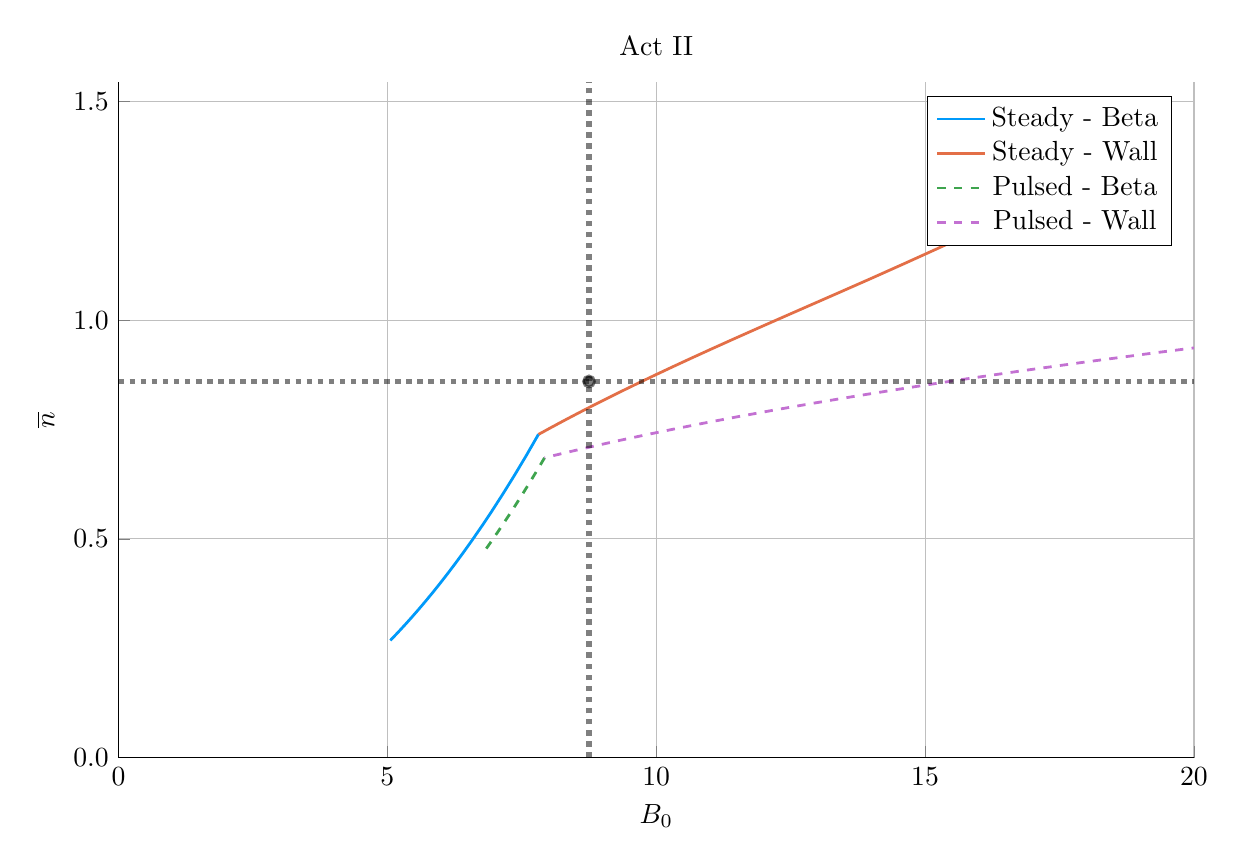
\begin{tikzpicture}[]
\begin{axis}[height = {101.6mm}, ylabel = {$\overline {n}$}, title = {Act II}, xmin = {0.0}, xmax = {20.0}, ymax = {1.5441728100587853}, xlabel = {${B}_{0}$}, {unbounded coords=jump, scaled x ticks = false, xticklabel style={rotate = 0}, xmajorgrids = true, xtick = {0.0,5.0,10.0,15.0,20.0}, xticklabels = {0,5,10,15,20}, xtick align = inside, axis lines* = left, scaled y ticks = false, yticklabel style={rotate = 0}, ymajorgrids = true, ytick = {0.0,0.5,1.0,1.5}, yticklabels = {0.0,0.5,1.0,1.5}, ytick align = inside, axis lines* = left,     xshift = 0.0mm,
    yshift = 0.0mm,
    axis background/.style={fill={rgb,1:red,1.00000000;green,1.00000000;blue,1.00000000}}
, colorbar style={title=}}, ymin = {0.0}, width = {152.4mm}]\addplot+ [color = {rgb,1:red,0.00000000;green,0.60560316;blue,0.97868012},
draw opacity=1.0,
line width=1,
solid,mark = none,
mark size = 2.0,
mark options = {
    color = {rgb,1:red,0.00000000;green,0.00000000;blue,0.00000000}, draw opacity = 1.0,
    fill = {rgb,1:red,0.00000000;green,0.60560316;blue,0.97868012}, fill opacity = 1.0,
    line width = 1,
    rotate = 0,
    solid
}]coordinates {
(7.810935944285959, 0.7392707051337243)
(7.57736049850867, 0.6893241315063908)
(7.354864292609041, 0.6436501709290285)
(7.145167234136329, 0.6021540921934464)
(6.9473303865083675, 0.5643735288542525)
(6.760499508614096, 0.5299053900882337)
(6.583897990324067, 0.49839753855041186)
(6.416817229618043, 0.46954134154583216)
(6.258609820663305, 0.4430656232049669)
(6.108683264880386, 0.4187315163971972)
(5.966494431410919, 0.3963281014258099)
(5.831544666176381, 0.3756686996634227)
(5.703375459679132, 0.35658771377800863)
(5.581564609582325, 0.3389379270681461)
(5.465722802994068, 0.3225881874025154)
(5.355490573482678, 0.3074214164440723)
(5.25053558682053, 0.29333289401274665)
(5.1505502068221745, 0.28022877494727205)
(5.0552493196883175, 0.2680248049954986)
};
\addlegendentry{Steady - Beta}
\addplot+ [color = {rgb,1:red,0.88887350;green,0.43564919;blue,0.27812294},
draw opacity=1.0,
line width=1,
solid,mark = none,
mark size = 2.0,
mark options = {
    color = {rgb,1:red,0.00000000;green,0.00000000;blue,0.00000000}, draw opacity = 1.0,
    fill = {rgb,1:red,0.88887350;green,0.43564919;blue,0.27812294}, fill opacity = 1.0,
    line width = 1,
    rotate = 0,
    solid
}]coordinates {
(17.25550839059296, 1.2868106750489878)
(16.594334962335296, 1.24304140812688)
(15.9071755430688, 1.2021404957706228)
(15.233983138507648, 1.1639818112748392)
(14.594239858921854, 1.1283888315904949)
(13.989673082630297, 1.0951391026120905)
(13.414782495717416, 1.0640043999097666)
(12.872659546281994, 1.03481943692435)
(12.364365715508608, 1.0074306882588195)
(11.889507953196574, 0.981695908134051)
(11.44685939646348, 0.9574844127563981)
(11.034739998180656, 0.9346767176305681)
(10.651252523287319, 0.9131638706730609)
(10.294428800132035, 0.8928466586873244)
(9.962319203963213, 0.8736347818299899)
(9.653045819449929, 0.8554460463225335)
(9.364832254395445, 0.8382056012507431)
(9.096018465506306, 0.8218452314414121)
(8.844373144802077, 0.8062990085169807)
(8.61055754360846, 0.7915212142227128)
(8.391192178573277, 0.7774487902511544)
(8.18577947665566, 0.7640378824815516)
(7.99323348423048, 0.7512449123451418)
(7.812301489248497, 0.7390284357328623)
};
\addlegendentry{Steady - Wall}
\addplot+ [color = {rgb,1:red,0.24222430;green,0.64327509;blue,0.30444865},
draw opacity=1.0,
line width=1,
dashed,mark = none,
mark size = 2.0,
mark options = {
    color = {rgb,1:red,0.00000000;green,0.00000000;blue,0.00000000}, draw opacity = 1.0,
    fill = {rgb,1:red,0.24222430;green,0.64327509;blue,0.30444865}, fill opacity = 1.0,
    line width = 1,
    rotate = 0,
    solid
}]coordinates {
(7.923668284887995, 0.6855708152865015)
(7.923668284887995, 0.6855708152865001)
(7.836759696043437, 0.6674976140211183)
(7.6662731560983355, 0.6327757462190718)
(7.50499428233835, 0.6008148243047226)
(7.35232773269976, 0.5713465611707179)
(7.207727224738343, 0.5441333400373862)
(7.070690693175276, 0.5189642181761778)
(6.940756001029682, 0.4956515120838104)
(6.817497143644154, 0.4740278724318922)
};
\addlegendentry{Pulsed - Beta}
\addplot+ [color = {rgb,1:red,0.76444018;green,0.44411178;blue,0.82429754},
draw opacity=1.0,
line width=1,
dashed,mark = none,
mark size = 2.0,
mark options = {
    color = {rgb,1:red,0.00000000;green,0.00000000;blue,0.00000000}, draw opacity = 1.0,
    fill = {rgb,1:red,0.76444018;green,0.44411178;blue,0.82429754}, fill opacity = 1.0,
    line width = 1,
    rotate = 0,
    solid
}]coordinates {
(22.56106430311702, 0.9746924566353471)
(20.85607192394036, 0.9498488456867051)
(19.335265246056654, 0.9264506756065961)
(17.974121547130903, 0.9043813484514631)
(16.751976718553127, 0.8835361767033411)
(15.651329744019142, 0.8638209298122244)
(14.65728744097675, 0.8451505842528242)
(13.757118584462601, 0.8274482459654839)
(12.939893642194303, 0.81064421844431)
(12.196191964860315, 0.7946751942861513)
(11.517862472405039, 0.7794835517545479)
(10.897827027335556, 0.7650167409549175)
(10.329918077124672, 0.7512267468036133)
(9.808743940706389, 0.7380696177777689)
(9.329576544487265, 0.7255050515455878)
(8.888257451278507, 0.7134960295716953)
(8.481118883411932, 0.7020084942050875)
(8.10491708701527, 0.6910110626520426)
(7.923668284887995, 0.6855708152865015)
(7.923668284887995, 0.6855708152865001)
};
\addlegendentry{Pulsed - Wall}
\addplot+ [color = {rgb,1:red,0.00000000;green,0.00000000;blue,0.00000000},
draw opacity=0.5,
line width=2,
dotted,mark = none,
mark size = 2.0,
mark options = {
    color = {rgb,1:red,0.00000000;green,0.00000000;blue,0.00000000}, draw opacity = 0.5,
    fill = {rgb,1:red,0.00000000;green,0.00000000;blue,0.00000000}, fill opacity = 0.5,
    line width = 1,
    rotate = 0,
    solid
},forget plot]coordinates {
(0.0, 0.86)
(20.0, 0.86)
};
\addplot+ [color = {rgb,1:red,0.00000000;green,0.00000000;blue,0.00000000},
draw opacity=0.5,
line width=2,
dotted,mark = none,
mark size = 2.0,
mark options = {
    color = {rgb,1:red,0.00000000;green,0.00000000;blue,0.00000000}, draw opacity = 0.5,
    fill = {rgb,1:red,0.00000000;green,0.00000000;blue,0.00000000}, fill opacity = 0.5,
    line width = 1,
    rotate = 0,
    solid
},forget plot]coordinates {
(8.75, 0.0)
(8.75, 1.5441728100587853)
};
\addplot+[draw=none, color = {rgb,1:red,0.00000000;green,0.00000000;blue,0.00000000},
draw opacity=0.5,
line width=0,
solid,mark = *,
mark size = 2.0,
mark options = {
    color = {rgb,1:red,0.00000000;green,0.00000000;blue,0.00000000}, draw opacity = 0.5,
    fill = {rgb,1:red,0.00000000;green,0.00000000;blue,0.00000000}, fill opacity = 0.5,
    line width = 1,
    rotate = 0,
    solid
},forget plot] coordinates {
(8.75, 0.86)
};
\end{axis}

\end{tikzpicture}

    \end{adjustbox}
        \caption{ACT II}
    \end{subfigure}
    \hfill \hfill ~\\ ~\\ ~\\ ~\\
  \caption[]{Magnet Scan: $\overline n$ vs $B_0$} ~\\

\end{figure*}


\clearpage

\newpage

\subsection*{ Plasma Current -- $I_P$ }
  \label{subsection:scan_I_P}

\begin{figure*}[h!]
    \centering
    \hfill
    \begin{subfigure}[t]{0.45\textwidth}
        \centering
    \begin{adjustbox}{width=\textwidth}
      \Large
      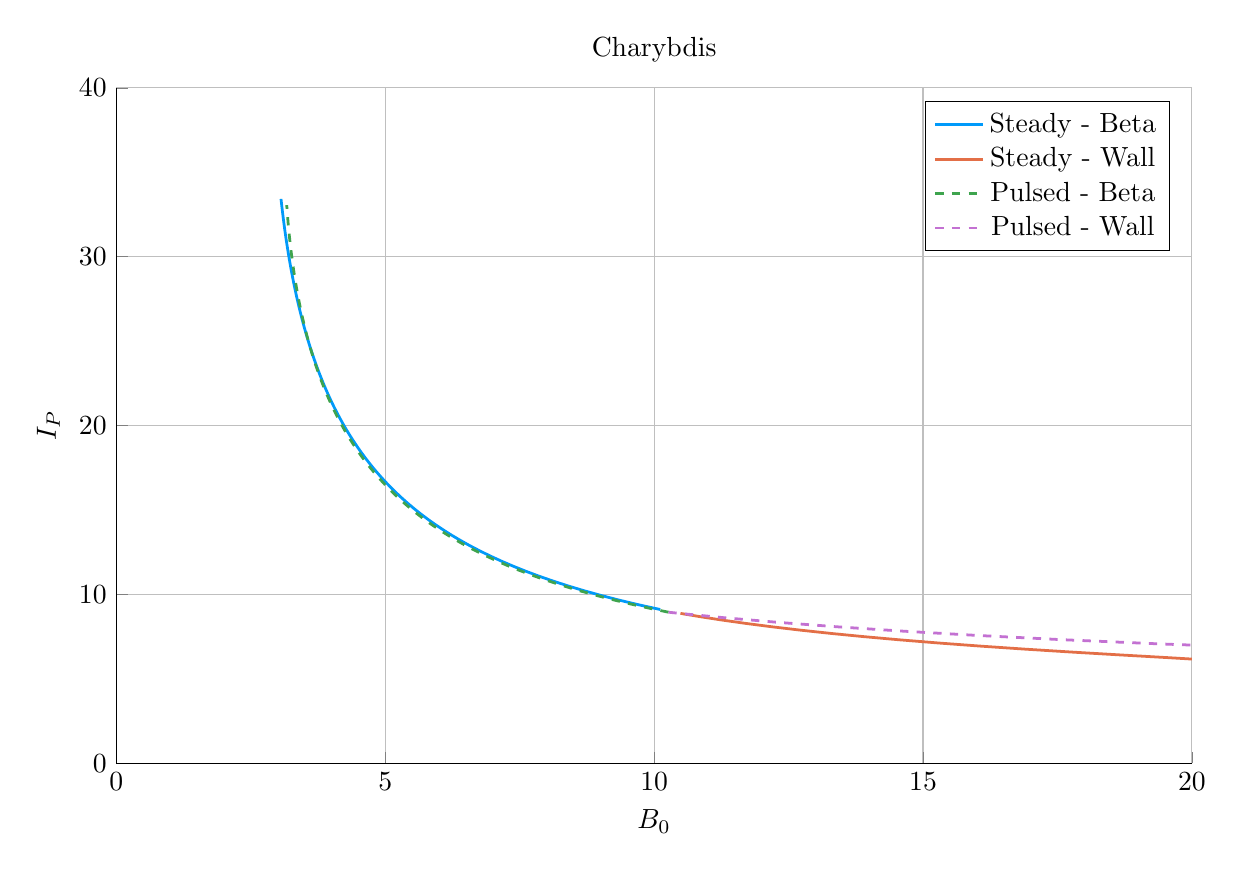
\begin{tikzpicture}[]
\begin{axis}[height = {101.6mm}, ylabel = {${I}_{P}$}, title = {Charybdis}, xmin = {0.0}, xmax = {20.0}, ymax = {40.0}, xlabel = {${B}_{0}$}, {unbounded coords=jump, scaled x ticks = false, xticklabel style={rotate = 0}, xmajorgrids = true, xtick = {0.0,5.0,10.0,15.0,20.0}, xticklabels = {0,5,10,15,20}, xtick align = inside, axis lines* = left, scaled y ticks = false, yticklabel style={rotate = 0}, ymajorgrids = true, ytick = {0.0,10.0,20.0,30.0,40.0}, yticklabels = {0,10,20,30,40}, ytick align = inside, axis lines* = left,     xshift = 0.0mm,
    yshift = 0.0mm,
    axis background/.style={fill={rgb,1:red,1.00000000;green,1.00000000;blue,1.00000000}}
, colorbar style={title=}}, ymin = {0.0}, width = {152.4mm}]\addplot+ [color = {rgb,1:red,0.00000000;green,0.60560316;blue,0.97868012},
draw opacity=1.0,
line width=1,
solid,mark = none,
mark size = 2.0,
mark options = {
    color = {rgb,1:red,0.00000000;green,0.00000000;blue,0.00000000}, draw opacity = 1.0,
    fill = {rgb,1:red,0.00000000;green,0.60560316;blue,0.97868012}, fill opacity = 1.0,
    line width = 1,
    rotate = 0,
    solid
}]coordinates {
(10.112818033153026, 9.109804749009676)
(9.722156888543116, 9.382660606439602)
(9.357875603858393, 9.658623066773757)
(9.017653755630063, 9.93763831806042)
(8.6995124437054, 10.219618817994236)
(8.401566530516865, 10.504519362744562)
(8.122163706328223, 10.792280677997171)
(7.859819415455661, 11.082843294085125)
(7.613196557650265, 11.376147621424183)
(7.381088038653343, 11.672134020523213)
(7.162401716104116, 11.97074286698656)
(6.956147367527331, 12.271914611882774)
(6.761425371986388, 12.575589837814922)
(6.577416849463348, 12.881709310995102)
(6.403375044688587, 13.190214029597128)
(6.2386177769852695, 13.501045268634927)
(6.0825208065966905, 13.81414462146812)
(5.934511989185341, 14.129454038897217)
(5.794066116682695, 14.446915864143662)
(5.660700347012839, 14.766472866417956)
(5.533970150598111, 15.088068271339658)
(5.413465705416883, 15.411645789210521)
(5.298808685607224, 15.737149640576702)
(5.189649392059402, 16.064524580680573)
(5.085664187259174, 16.393715920921032)
(4.986553195072601, 16.724669548961394)
(4.892038235455667, 17.05733194697)
(4.801860966679364, 17.391650208196687)
(4.7157812114040425, 17.727572051978182)
(4.633575445956479, 18.065045837259397)
(4.5550354347559185, 18.404020574713467)
(4.479966994069385, 18.744445937537844)
(4.408188871204256, 19.08627227100042)
(4.33953172691477, 19.429450600805218)
(4.273837210246432, 19.773932640343546)
(4.210957116299974, 20.119670796892883)
(4.15075261849161, 20.466618176823495)
(4.0930935678432965, 20.814728589868544)
(4.037857852672517, 21.16395655251145)
(3.9849308127842145, 21.514257290541156)
(3.9342047029103653, 21.86558674082401)
(3.8855782007091695, 22.217901552337885)
(3.838955955133626, 22.57115908651246)
(3.7942481714200484, 22.925317416916894)
(3.7513702293348077, 23.280335328335426)
(3.710242331663442, 23.636172315267423)
(3.6707891802306123, 23.992788579888426)
(3.6329396770109583, 24.35014502950619)
(3.5966266481325166, 24.708203273544143)
(3.5617865887889004, 25.066925620083293)
(3.5283594272686503, 25.42627507199144)
(3.496288306480746, 25.786215322669122)
(3.465519381509793, 26.14671075143667)
(3.4360016318699595, 26.507726418589996)
(3.4076866872513096, 26.869228060147776)
(3.380528665662031, 27.23118208231289)
(3.3544840229690007, 27.59355555567121)
(3.3295114129297314, 27.95631620914659)
(3.3055715568879336, 28.319432423733286)
(3.2826271223788512, 28.682873226023403)
(3.260642607548369, 29.046608285900476)
(3.239584247604666, 29.410607887946366)
(3.2194198921826622, 29.774842967985702)
(3.2001189373344725, 30.13928506243539)
(3.181652227422265, 30.50390632282234)
(3.163991977015565, 30.868679504072222)
(3.1471116955378684, 31.233577957053683)
(3.130986116696265, 31.598575621036407)
(3.115591132350856, 31.963647016074752)
(3.1009037305081053, 32.328767235327966)
(3.0869019371473265, 32.69391193732724)
(3.0735647616124355, 33.05905733819915)
(3.0608721453218655, 33.42418020385512)
};
\addlegendentry{Steady - Beta}
\addplot+ [color = {rgb,1:red,0.88887350;green,0.43564919;blue,0.27812294},
draw opacity=1.0,
line width=1,
solid,mark = none,
mark size = 2.0,
mark options = {
    color = {rgb,1:red,0.00000000;green,0.00000000;blue,0.00000000}, draw opacity = 1.0,
    fill = {rgb,1:red,0.88887350;green,0.43564919;blue,0.27812294}, fill opacity = 1.0,
    line width = 1,
    rotate = 0,
    solid
}]coordinates {
(20.758867641064707, 5.985799665822783)
(20.346250098246923, 6.108942493532681)
(19.57104597888471, 6.2566628901192)
(18.681781921115476, 6.417629098853787)
(17.775790175980152, 6.587165743051122)
(16.896654716492492, 6.7628181854268625)
(16.063927450323227, 6.943127867636776)
(15.285557510665852, 7.127139792603281)
(14.563500533069154, 7.314189536626925)
(13.896568848875791, 7.503794928434107)
(13.281970890030232, 7.695595065247222)
(12.716170469467318, 7.889313314197647)
(12.195372283741088, 8.08473356459841)
(11.715794270833433, 8.28168430853991)
(11.273815669498969, 8.480027597476955)
(10.866051794088186, 8.67965116743724)
(10.489365023931143, 8.880465756900596)
};
\addlegendentry{Steady - Wall}
\addplot+ [color = {rgb,1:red,0.24222430;green,0.64327509;blue,0.30444865},
draw opacity=1.0,
line width=1,
dashed,mark = none,
mark size = 2.0,
mark options = {
    color = {rgb,1:red,0.00000000;green,0.00000000;blue,0.00000000}, draw opacity = 1.0,
    fill = {rgb,1:red,0.24222430;green,0.64327509;blue,0.30444865}, fill opacity = 1.0,
    line width = 1,
    rotate = 0,
    solid
}]coordinates {
(10.26788634689966, 8.948888331394)
(9.953967652326213, 9.156517417487386)
(9.567926244368271, 9.431254094087237)
(9.207974394987358, 9.709138284127413)
(8.871841888699304, 9.990106554082725)
(8.557505525932248, 10.274094131297865)
(8.263156925406376, 10.561035026718695)
(7.9871752024348766, 10.850862153690285)
(7.728103682045175, 11.143507444143625)
(7.484629973620137, 11.438901961835837)
(7.255568856523303, 11.736976012792741)
(7.039847526735421, 12.037659252992201)
(6.836492834698909, 12.34088079329773)
(6.644620209081183, 12.646569301626505)
(6.463424013335149, 12.954653102316353)
(6.2921691243175495, 13.265060272640811)
(6.13018355681404, 13.57771873640978)
(5.97685198655569, 13.892556354410377)
(5.831610044919842, 14.209501012655426)
(5.693939286027163, 14.528480705748802)
(5.563362729090489, 14.849423618771374)
(5.439440906144732, 15.17225820499948)
(5.321768347746793, 15.496913260556838)
(5.209970453003084, 15.823317994954149)
(5.103700692769835, 16.151402099512886)
(5.002638109938164, 16.48109581082738)
(4.906485077678376, 16.81232997135543)
(4.814965286571576, 17.145036086241255)
(4.727821933804548, 17.479146376497447)
(4.644816091323922, 17.814593828539103)
(4.565725232806084, 18.151312240074667)
(4.490341901840154, 18.48923626237099)
(4.418472505906755, 18.828301438923475)
(4.349936222622964, 19.168444240572487)
(4.284564006352339, 19.509602097122148)
(4.222197684694192, 19.85171342552675)
(4.162689135592264, 20.194717654723146)
(4.105899536872315, 20.53855524719695)
(4.051698680949713, 20.88316771738083)
(3.9999643482627323, 21.228497646992423)
(3.9505817337017928, 21.574488697425913)
(3.903442920928527, 21.92108561932238)
(3.858446400032002, 22.26823425944567)
(3.8154966244515616, 22.615881565000002)
(3.7745036035252744, 22.963975585526896)
(3.7353825273991994, 23.312465472525417)
(3.6980534213689746, 23.66130147693931)
(3.6624408270205375, 24.010434944658396)
(3.62847350780097, 24.35981831018104)
(3.5960841768845415, 24.70940508858472)
(3.565209245407392, 25.059149865951287)
(3.5357885893311605, 25.40900828839029)
(3.5077653333614305, 25.758937049803013)
(3.4810856504959875, 26.10889387852531)
(3.4556985759109375, 26.45883752298476)
(3.4315558340122845, 26.80872773650233)
(3.408611677587535, 27.158525261365455)
(3.3868227380888998, 27.508191812292555)
(3.36614788616562, 27.85769005940574)
(3.3465481016421226, 28.20698361082019)
(3.327986352208224, 28.556036994955615)
(3.3104274769652595, 28.904815649094107)
(3.2938380965241474, 29.253285869285435)
(3.278186482171801, 29.601414856656447)
(3.263442495132517, 29.949170635252603)
(3.2495774839156075, 30.296522066434655)
(3.236564206241785, 30.643438824926758)
(3.224376752844934, 30.989891381566444)
(3.212990475972638, 31.33585098638364)
(3.2023819222517877, 31.68128965205573)
(3.192528769611062, 32.02618013778299)
(3.1834097679780142, 32.3704959336189)
(3.1750046834890777, 32.71421124528863)
(3.1672942459724482, 33.05730097952028)
};
\addlegendentry{Pulsed - Beta}
\addplot+ [color = {rgb,1:red,0.76444018;green,0.44411178;blue,0.82429754},
draw opacity=1.0,
line width=1,
dashed,mark = none,
mark size = 2.0,
mark options = {
    color = {rgb,1:red,0.00000000;green,0.00000000;blue,0.00000000}, draw opacity = 1.0,
    fill = {rgb,1:red,0.76444018;green,0.44411178;blue,0.82429754}, fill opacity = 1.0,
    line width = 1,
    rotate = 0,
    solid
}]coordinates {
(48.990476413653056, 5.233231306533011)
(42.83950920694117, 5.450620283665572)
(37.687790427214495, 5.6718702016173905)
(33.33937742845888, 5.896960389954213)
(29.64296398154308, 6.125865899853728)
(26.48039367255613, 6.3585577989883495)
(23.758442882319894, 6.595003439225416)
(21.402860298405816, 6.835166701033339)
(19.353987387634486, 7.079008217935534)
(17.563502020363714, 7.326485583949076)
(15.991970371213752, 7.577553546297115)
(14.606987499719377, 7.832164185672022)
(13.381751501116137, 8.090267085664676)
(12.293960329570087, 8.351809492897173)
(11.32495111804522, 8.616736469096852)
(10.459023415380802, 8.88499103615607)
(10.26788634689966, 8.948888331394)
};
\addlegendentry{Pulsed - Wall}
\end{axis}

\end{tikzpicture}

    \end{adjustbox}
        \caption{Charybdis}
    \end{subfigure}
    \hfill
    \begin{subfigure}[t]{0.45\textwidth}
        \centering
    \begin{adjustbox}{width=\textwidth}
      \Large
      \begin{tikzpicture}[]
\begin{axis}[height = {101.6mm}, ylabel = {${I}_{P}$}, title = {Proteus}, xmin = {0.0}, xmax = {20.0}, ymax = {40.0}, xlabel = {${B}_{0}$}, {unbounded coords=jump, scaled x ticks = false, xticklabel style={rotate = 0}, xmajorgrids = true, xtick = {0.0,5.0,10.0,15.0,20.0}, xticklabels = {0,5,10,15,20}, xtick align = inside, axis lines* = left, scaled y ticks = false, yticklabel style={rotate = 0}, ymajorgrids = true, ytick = {0.0,10.0,20.0,30.0,40.0}, yticklabels = {0,10,20,30,40}, ytick align = inside, axis lines* = left,     xshift = 0.0mm,
    yshift = 0.0mm,
    axis background/.style={fill={rgb,1:red,1.00000000;green,1.00000000;blue,1.00000000}}
, colorbar style={title=}}, ymin = {0.0}, width = {152.4mm}]\addplot+ [color = {rgb,1:red,0.00000000;green,0.60560316;blue,0.97868012},
draw opacity=1.0,
line width=1,
solid,mark = none,
mark size = 2.0,
mark options = {
    color = {rgb,1:red,0.00000000;green,0.00000000;blue,0.00000000}, draw opacity = 1.0,
    fill = {rgb,1:red,0.00000000;green,0.60560316;blue,0.97868012}, fill opacity = 1.0,
    line width = 1,
    rotate = 0,
    solid
}]coordinates {
(4.658732060637907, 36.50370025334007)
(4.211109766361548, 28.793098053082183)
(3.9293920326356777, 24.06490545444949)
(3.7651903683456465, 21.10045089594333)
(3.6776039543745567, 19.16244941990859)
(3.6402437753208394, 17.846461952491417)
(3.6366994671255806, 16.926276879950834)
(3.656621534643579, 16.269746547180418)
(3.693300156736026, 15.796056852217028)
(3.7422515017241134, 15.453649642413087)
(3.865532743079537, 15.036837060372921)
(3.936096932264377, 14.922569221711694)
(4.010907188015084, 14.8536572087352)
(4.089072356933184, 14.821299160535771)
(4.169903401491354, 14.818861401886512)
(4.252857906625248, 14.841256611964031)
(4.337501757261618, 14.884522476430423)
(4.42348218754058, 14.945529897312955)
(4.5983381267510195, 15.111240396853018)
(4.686766232902671, 15.212267911916946)
(4.775618142770625, 15.323497142689403)
(4.864743502376605, 15.443795527589858)
(4.927312314219091, 15.533016055936583)
};
\addlegendentry{Pulsed - Kink}
\addplot+ [color = {rgb,1:red,0.88887350;green,0.43564919;blue,0.27812294},
draw opacity=1.0,
line width=1,
solid,mark = none,
mark size = 2.0,
mark options = {
    color = {rgb,1:red,0.00000000;green,0.00000000;blue,0.00000000}, draw opacity = 1.0,
    fill = {rgb,1:red,0.88887350;green,0.43564919;blue,0.27812294}, fill opacity = 1.0,
    line width = 1,
    rotate = 0,
    solid
}]coordinates {
(4.927312314219091, 15.533016055936583)
(4.984545814413324, 15.557706707103696)
(5.17452482724068, 15.647479871719217)
(5.362091669637646, 15.747624196363061)
(5.54700293215903, 15.857321778193958)
(5.729042482638278, 15.975861255207144)
(5.908022832274664, 16.102618075838613)
(6.083785777786694, 16.237038956073114)
(6.256202341425288, 16.378629623384892)
(6.324169421042356, 16.43713817031406)
};
\addlegendentry{Pulsed - Beta}
\addplot+ [color = {rgb,1:red,0.24222430;green,0.64327509;blue,0.30444865},
draw opacity=1.0,
line width=1,
solid,mark = none,
mark size = 2.0,
mark options = {
    color = {rgb,1:red,0.00000000;green,0.00000000;blue,0.00000000}, draw opacity = 1.0,
    fill = {rgb,1:red,0.24222430;green,0.64327509;blue,0.30444865}, fill opacity = 1.0,
    line width = 1,
    rotate = 0,
    solid
}]coordinates {
(6.324169421042356, 16.43713817031406)
(6.727338549778396, 16.428362526295228)
(7.320469048424473, 16.46587695659026)
(7.835746509376305, 16.549637387770833)
(8.290245520072391, 16.666047192319372)
(8.696162676727877, 16.806645632971204)
(9.0624397222742, 16.96586952003378)
(9.395798186463841, 17.139893061774544)
(9.701405747258567, 17.325986304924154)
(10.244760202900984, 17.72683799874801)
(10.930275827723788, 18.381659224761872)
(11.131878682735255, 18.611003943311434)
(11.50278450645086, 19.083143567152845)
(11.83715172742864, 19.570796942651278)
(11.992609772603878, 19.819732975920697)
(12.141110720831467, 20.071776280624523)
};
\addlegendentry{Pulsed - Wall}
\end{axis}

\end{tikzpicture}

    \end{adjustbox}
        \caption{Proteus}
    \end{subfigure}
    \hfill \hfill ~\\ ~\\ ~\\ ~\\
    \hfill
    \begin{subfigure}[t]{0.45\textwidth}
        \centering
    \begin{adjustbox}{width=\textwidth}
      \Large
      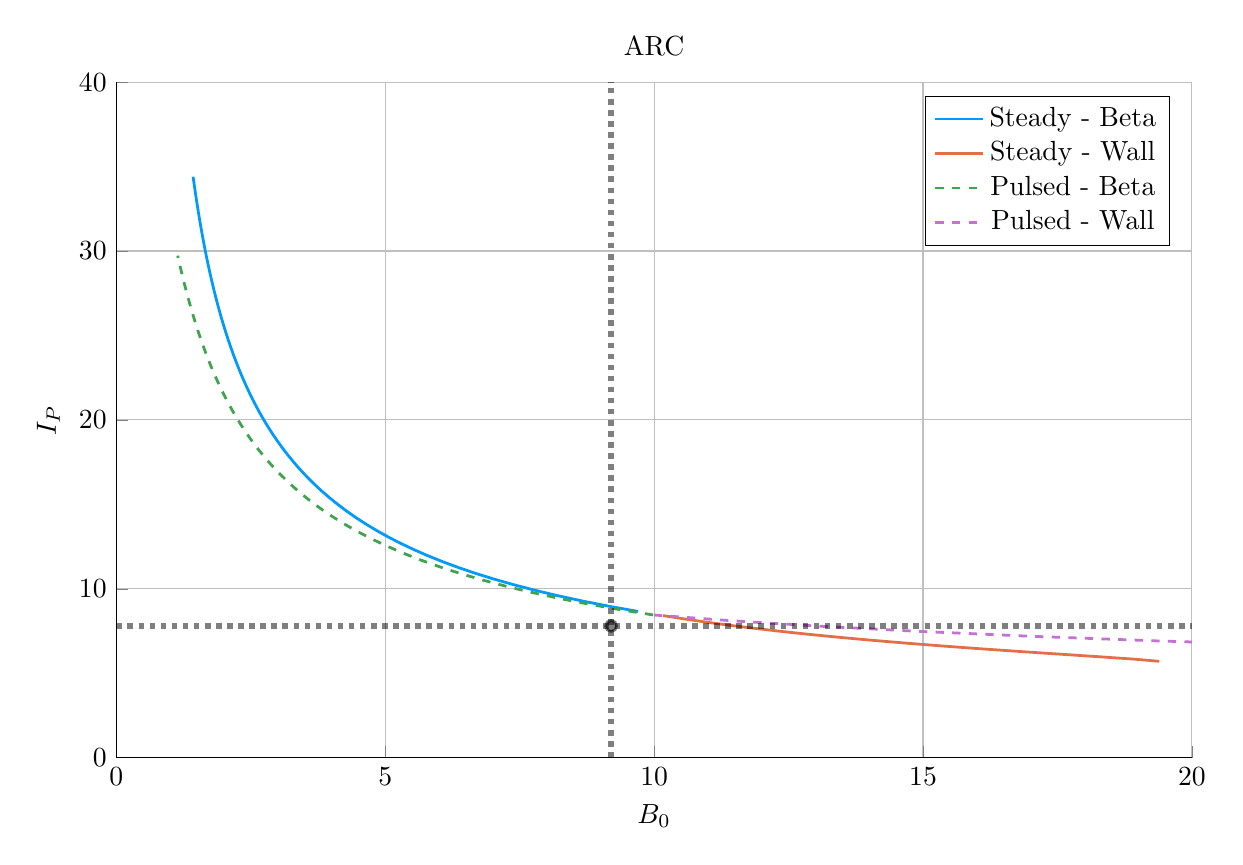
\begin{tikzpicture}[]
\begin{axis}[height = {101.6mm}, ylabel = {${I}_{P}$}, title = {ARC}, xmin = {0.0}, xmax = {20.0}, ymax = {40.0}, xlabel = {${B}_{0}$}, {unbounded coords=jump, scaled x ticks = false, xticklabel style={rotate = 0}, xmajorgrids = true, xtick = {0.0,5.0,10.0,15.0,20.0}, xticklabels = {0,5,10,15,20}, xtick align = inside, axis lines* = left, scaled y ticks = false, yticklabel style={rotate = 0}, ymajorgrids = true, ytick = {0.0,10.0,20.0,30.0,40.0}, yticklabels = {0,10,20,30,40}, ytick align = inside, axis lines* = left,     xshift = 0.0mm,
    yshift = 0.0mm,
    axis background/.style={fill={rgb,1:red,1.00000000;green,1.00000000;blue,1.00000000}}
, colorbar style={title=}}, ymin = {0.0}, width = {152.4mm}]\addplot+ [color = {rgb,1:red,0.00000000;green,0.60560316;blue,0.97868012},
draw opacity=1.0,
line width=1,
solid,mark = none,
mark size = 2.0,
mark options = {
    color = {rgb,1:red,0.00000000;green,0.00000000;blue,0.00000000}, draw opacity = 1.0,
    fill = {rgb,1:red,0.00000000;green,0.60560316;blue,0.97868012}, fill opacity = 1.0,
    line width = 1,
    rotate = 0,
    solid
}]coordinates {
(9.701206080853105, 8.658343870907427)
(9.162315904693079, 8.964855141636448)
(8.664301107137337, 9.277118721367206)
(8.203576462497304, 9.595036914426)
(7.776718537485166, 9.918585776352757)
(7.380720231870917, 10.247718935951552)
(7.012886014999712, 10.582387319200262)
(6.670795005901889, 10.922539274323045)
(6.352268997292712, 11.26812069483817)
(6.055344682097163, 11.61907514056121)
(5.778249464564785, 11.975343956529299)
(5.519380338856715, 12.336866389803589)
(5.2772854007125325, 12.703579704100664)
(5.050647625972996, 13.07541929220057)
(4.838270606140816, 13.452318786079019)
(4.639065978019038, 13.834210164711733)
(4.4520423235376105, 14.221023859501257)
(4.276295348572609, 14.61268885728139)
(4.110999177018484, 15.009132800857182)
(3.9553986195015125, 15.410282087044596)
(3.8088022956698633, 15.816061962178953)
(3.6705765055641186, 16.226396615066992)
(3.54013975965751, 16.64120926736311)
(3.4169578891619192, 17.060422261356294)
(3.30053966845824, 17.483957145159597)
(3.1904328903033052, 17.91173475530017)
(3.086220842019516, 18.343675296712746)
(2.9875191373772063, 18.77969842014449)
(2.8939728644914635, 19.2197232969848)
(2.8052540149097247, 19.663668691537165)
(2.7210591632720242, 20.11145303075519)
(2.6411073705789065, 20.562994471468567)
(2.565138287279709, 21.018210965128485)
(2.492910435164382, 21.477020320105293)
(2.4241996494611984, 21.939340261574117)
(2.3587976646588236, 22.405088489026962)
(2.296510829425685, 22.874182731452617)
(2.237158937627476, 23.34654080022686)
(2.180574163874242, 23.82208063975841)
(2.126600093288366, 24.300720375936947)
(2.075090836295778, 24.782378362431352)
(2.0259102202234582, 25.26697322488704)
(1.978931050353818, 25.754423903072542)
(1.9340344338545452, 26.244649691026318)
(1.8911091606836798, 26.737570275254438)
(1.8500511361739687, 27.233105771031717)
(1.8107628605384507, 27.731176756857092)
(1.773152951016952, 28.23170430711659)
(1.7371357028100902, 28.734610023004112)
(1.7026306853269466, 29.23981606175298)
(1.6695623706125668, 29.747245164229085)
(1.6378597911249178, 30.256820680936514)
(1.607456224302725, 30.768466596486252)
(1.5782889016090462, 31.282107552577845)
(1.5502987399539199, 31.797668869543177)
(1.5234300935954943, 32.31507656650066)
(1.4976305247952577, 32.83425738016771)
(1.4728505916614916, 33.35513878237846)
(1.4490436517578602, 33.87764899635294)
(1.4261656801829077, 34.40171701176134)
};
\addlegendentry{Steady - Beta}
\addplot+ [color = {rgb,1:red,0.88887350;green,0.43564919;blue,0.27812294},
draw opacity=1.0,
line width=1,
solid,mark = none,
mark size = 2.0,
mark options = {
    color = {rgb,1:red,0.00000000;green,0.00000000;blue,0.00000000}, draw opacity = 1.0,
    fill = {rgb,1:red,0.88887350;green,0.43564919;blue,0.27812294}, fill opacity = 1.0,
    line width = 1,
    rotate = 0,
    solid
}]coordinates {
(19.394007482712425, 5.705363947896813)
(18.932196567189358, 5.831631927327359)
(18.296989378345195, 5.971358416795512)
(17.587029315408756, 6.120248050030096)
(16.847882407994106, 6.27635241161913)
(16.111374502564406, 6.438084943966173)
(15.396027314547156, 6.6043437111573775)
(14.710952688793137, 6.774432932493379)
(14.06168447794857, 6.9477586358526295)
(13.450465418483889, 7.123875039246037)
(12.877644538645335, 7.302428845502918)
(12.342394470642008, 7.483135839919747)
(11.843182246608265, 7.66576464137543)
(11.376441269625893, 7.850323804140159)
(10.944966372727551, 8.036059275223955)
(10.541663878705513, 8.223435700494395)
(10.165908182236457, 8.412159667095638)
};
\addlegendentry{Steady - Wall}
\addplot+ [color = {rgb,1:red,0.24222430;green,0.64327509;blue,0.30444865},
draw opacity=1.0,
line width=1,
dashed,mark = none,
mark size = 2.0,
mark options = {
    color = {rgb,1:red,0.00000000;green,0.00000000;blue,0.00000000}, draw opacity = 1.0,
    fill = {rgb,1:red,0.24222430;green,0.64327509;blue,0.30444865}, fill opacity = 1.0,
    line width = 1,
    rotate = 0,
    solid
}]coordinates {
(9.980483622051658, 8.45211123232532)
(9.392786903460065, 8.749174237506722)
(8.79273598103983, 9.084875445329175)
(8.23820290909994, 9.429466194729264)
(7.725182218401588, 9.783065958753857)
(7.250078106370205, 10.145791398086809)
(6.80965553466646, 10.517756265001724)
(6.400998063035608, 10.899071333792335)
(6.0214713600430425, 11.28984436597908)
(5.668691517461799, 11.690180120182706)
(5.340497445229901, 12.100180418434789)
(5.034926745580058, 12.519944282916168)
(4.750194564008521, 12.949568159742276)
(4.484674995755211, 13.389146249526421)
(4.236884692979903, 13.838770968145022)
(4.00546837264544, 14.298533565526986)
(3.7891859704718387, 14.768524935556082)
(3.5869012239550364, 15.2488366565296)
(3.3975714987448393, 15.739562309352701)
(3.2202386987489797, 16.240799130174846)
(3.0540211220494466, 16.752650066058415)
(2.8981061427709687, 17.27522631730515)
(2.7517436139566023, 17.808650469386293)
(2.6142398986781377, 18.353060342640163)
(2.4849524463010138, 18.908613721362002)
(2.363284838174807, 19.475494169025602)
(2.248682232019848, 20.053918198206937)
(2.140627136740878, 20.644144149900036)
(2.038635448877246, 21.246483258877372)
(1.9422526775794744, 21.861313557471373)
(1.8510502754751532, 22.48909752802998)
(1.7646219756564088, 23.130404800381292)
(1.6825800061969869, 23.785941781633092)
(1.6045510059627948, 24.456591033172632)
(1.53017138625397, 25.143464707502787)
(1.4590817483192686, 25.84797885666414)
(1.3909197311384796, 26.571959755666764)
(1.3253102336217724, 27.3178012356156)
(1.261851128383913, 28.088707029156687)
(1.20009089049112, 28.889082725820668)
(1.1394908096975784, 29.725209471035893)
};
\addlegendentry{Pulsed - Beta}
\addplot+ [color = {rgb,1:red,0.76444018;green,0.44411178;blue,0.82429754},
draw opacity=1.0,
line width=1,
dashed,mark = none,
mark size = 2.0,
mark options = {
    color = {rgb,1:red,0.00000000;green,0.00000000;blue,0.00000000}, draw opacity = 1.0,
    fill = {rgb,1:red,0.76444018;green,0.44411178;blue,0.82429754}, fill opacity = 1.0,
    line width = 1,
    rotate = 0,
    solid
}]coordinates {
(29.27715761652869, 6.106956435644008)
(25.4410619834368, 6.368429153074452)
(22.158819835998365, 6.637611037727747)
(19.342453256965573, 6.914640849606676)
(16.919364280634177, 7.199655680909235)
(14.829378672669455, 7.492790823032018)
(13.022412368922526, 7.794179619860046)
(11.456617692058645, 8.103953307930404)
(10.096901921254785, 8.422240844292133)
(9.980483622051658, 8.45211123232532)
};
\addlegendentry{Pulsed - Wall}
\addplot+ [color = {rgb,1:red,0.00000000;green,0.00000000;blue,0.00000000},
draw opacity=0.5,
line width=2,
dotted,mark = none,
mark size = 2.0,
mark options = {
    color = {rgb,1:red,0.00000000;green,0.00000000;blue,0.00000000}, draw opacity = 0.5,
    fill = {rgb,1:red,0.00000000;green,0.00000000;blue,0.00000000}, fill opacity = 0.5,
    line width = 1,
    rotate = 0,
    solid
},forget plot]coordinates {
(0.0, 7.8)
(20.0, 7.8)
};
\addplot+ [color = {rgb,1:red,0.00000000;green,0.00000000;blue,0.00000000},
draw opacity=0.5,
line width=2,
dotted,mark = none,
mark size = 2.0,
mark options = {
    color = {rgb,1:red,0.00000000;green,0.00000000;blue,0.00000000}, draw opacity = 0.5,
    fill = {rgb,1:red,0.00000000;green,0.00000000;blue,0.00000000}, fill opacity = 0.5,
    line width = 1,
    rotate = 0,
    solid
},forget plot]coordinates {
(9.2, 0.0)
(9.2, 40.0)
};
\addplot+[draw=none, color = {rgb,1:red,0.00000000;green,0.00000000;blue,0.00000000},
draw opacity=0.5,
line width=0,
solid,mark = *,
mark size = 2.0,
mark options = {
    color = {rgb,1:red,0.00000000;green,0.00000000;blue,0.00000000}, draw opacity = 0.5,
    fill = {rgb,1:red,0.00000000;green,0.00000000;blue,0.00000000}, fill opacity = 0.5,
    line width = 1,
    rotate = 0,
    solid
},forget plot] coordinates {
(9.2, 7.8)
};
\end{axis}

\end{tikzpicture}

    \end{adjustbox}
        \caption{ARC}
    \end{subfigure}
    \hfill
    \begin{subfigure}[t]{0.45\textwidth}
        \centering
    \begin{adjustbox}{width=\textwidth}
      \Large
      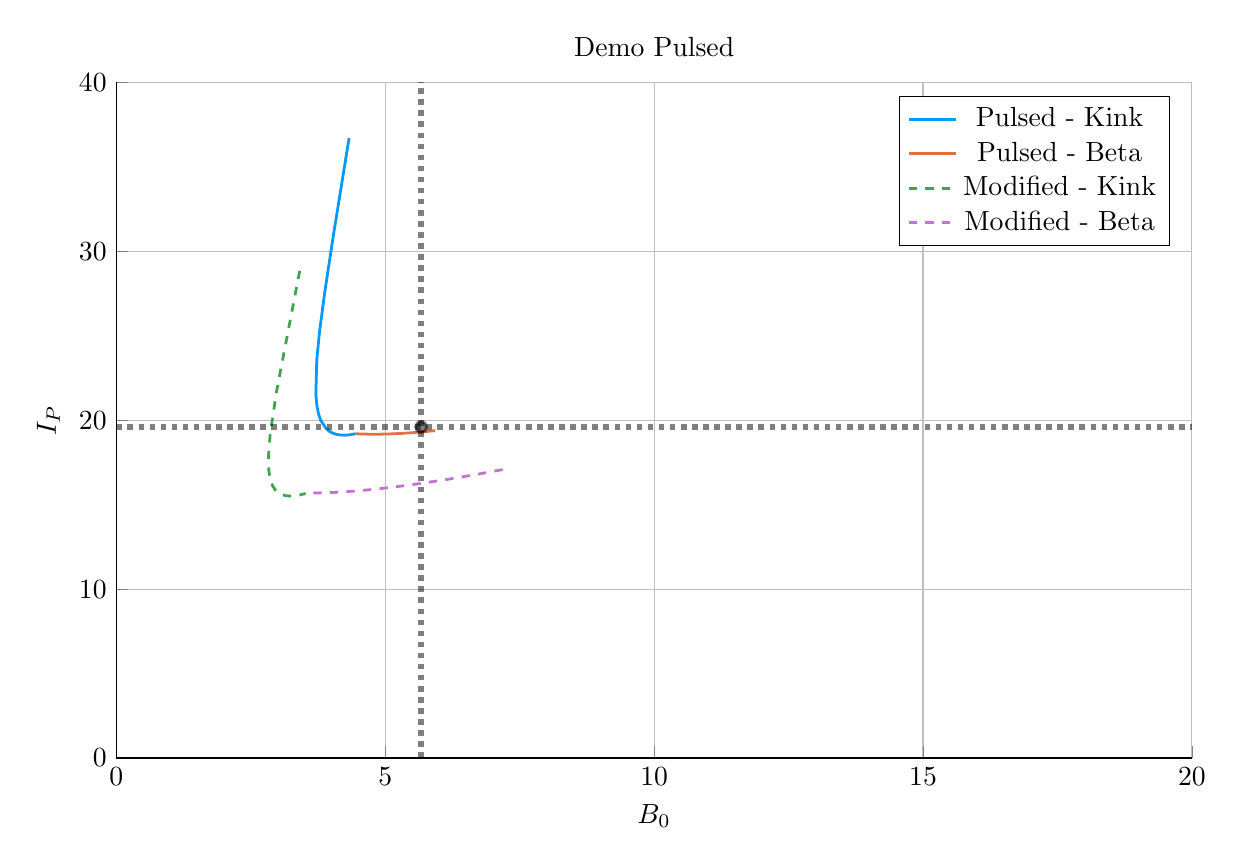
\begin{tikzpicture}[]
\begin{axis}[height = {101.6mm}, ylabel = {${I}_{P}$}, title = {Demo Pulsed}, xmin = {0.0}, xmax = {20.0}, ymax = {40.0}, xlabel = {${B}_{0}$}, {unbounded coords=jump, scaled x ticks = false, xticklabel style={rotate = 0}, xmajorgrids = true, xtick = {0.0,5.0,10.0,15.0,20.0}, xticklabels = {0,5,10,15,20}, xtick align = inside, axis lines* = left, scaled y ticks = false, yticklabel style={rotate = 0}, ymajorgrids = true, ytick = {0.0,10.0,20.0,30.0,40.0}, yticklabels = {0,10,20,30,40}, ytick align = inside, axis lines* = left,     xshift = 0.0mm,
    yshift = 0.0mm,
    axis background/.style={fill={rgb,1:red,1.00000000;green,1.00000000;blue,1.00000000}}
, colorbar style={title=}}, ymin = {0.0}, width = {152.4mm}]\addplot+ [color = {rgb,1:red,0.00000000;green,0.60560316;blue,0.97868012},
draw opacity=1.0,
line width=1,
solid,mark = none,
mark size = 2.0,
mark options = {
    color = {rgb,1:red,0.00000000;green,0.00000000;blue,0.00000000}, draw opacity = 1.0,
    fill = {rgb,1:red,0.00000000;green,0.60560316;blue,0.97868012}, fill opacity = 1.0,
    line width = 1,
    rotate = 0,
    solid
}]coordinates {
(4.327031075670194, 36.71051032912112)
(4.038214026054326, 31.014995367356207)
(3.8713719163129245, 27.51734786322149)
(3.7758613845615545, 25.19534286389616)
(3.7257856761317214, 23.57285610926683)
(3.7090473695925437, 21.52905816503197)
(3.727711597554826, 20.874444053021588)
(3.7586131667481433, 20.377542510464334)
(3.799052518631718, 19.99951688957442)
(3.901290136389271, 19.499202175706746)
(3.960577465316514, 19.343044014643887)
(4.0241209645210345, 19.233955791269285)
(4.0912717805663785, 19.16365729524907)
(4.161514602943343, 19.125701869840853)
(4.2344343960723005, 19.11499858904485)
(4.309692554546368, 19.127475979338943)
(4.450417240491067, 19.198383823705257)
};
\addlegendentry{Pulsed - Kink}
\addplot+ [color = {rgb,1:red,0.88887350;green,0.43564919;blue,0.27812294},
draw opacity=1.0,
line width=1,
solid,mark = none,
mark size = 2.0,
mark options = {
    color = {rgb,1:red,0.00000000;green,0.00000000;blue,0.00000000}, draw opacity = 1.0,
    fill = {rgb,1:red,0.88887350;green,0.43564919;blue,0.27812294}, fill opacity = 1.0,
    line width = 1,
    rotate = 0,
    solid
}]coordinates {
(4.450417240491067, 19.198383823705257)
(4.490148631384312, 19.192414153878335)
(4.692490181445514, 19.174087186739918)
(4.8960344619053355, 19.17397121853779)
(5.100651132702229, 19.189978018951553)
(5.306202822090688, 19.220357277326283)
(5.512545696627038, 19.263633100211838)
(5.719530043226767, 19.31855421750887)
(5.927000883375481, 19.384054548489104)
};
\addlegendentry{Pulsed - Beta}
\addplot+ [color = {rgb,1:red,0.24222430;green,0.64327509;blue,0.30444865},
draw opacity=1.0,
line width=1,
dashed,mark = none,
mark size = 2.0,
mark options = {
    color = {rgb,1:red,0.00000000;green,0.00000000;blue,0.00000000}, draw opacity = 1.0,
    fill = {rgb,1:red,0.24222430;green,0.64327509;blue,0.30444865}, fill opacity = 1.0,
    line width = 1,
    rotate = 0,
    solid
}]coordinates {
(3.4087424183072135, 28.845639077165217)
(2.977074181068944, 21.687713986294685)
(2.8592500074202523, 19.170340224057398)
(2.827199220063259, 17.83397336320386)
(2.8339789008667826, 17.01478565989059)
(2.862412302880871, 16.477486603636205)
(2.9044598258085443, 16.113958654578386)
(2.95577893007882, 15.866460603971907)
(3.0137895352525907, 15.700928946757587)
(3.076849710218805, 15.59578560596909)
(3.1438583711612704, 15.536607983152381)
(3.214045733980633, 15.513342675582972)
(3.2868548955983727, 15.518740955012225)
(3.361871149981842, 15.547428978968492)
(3.4387778750377818, 15.595329068459918)
(3.5173279629378453, 15.659285368310089)
};
\addlegendentry{Modified - Kink}
\addplot+ [color = {rgb,1:red,0.76444018;green,0.44411178;blue,0.82429754},
draw opacity=1.0,
line width=1,
dashed,mark = none,
mark size = 2.0,
mark options = {
    color = {rgb,1:red,0.00000000;green,0.00000000;blue,0.00000000}, draw opacity = 1.0,
    fill = {rgb,1:red,0.76444018;green,0.44411178;blue,0.82429754}, fill opacity = 1.0,
    line width = 1,
    rotate = 0,
    solid
}]coordinates {
(3.6607028750648505, 15.691192911261952)
(3.8574448036470477, 15.70165788278533)
(4.056375867871351, 15.726578234093749)
(4.257366397480293, 15.764127054896537)
(4.460279103534801, 15.812802650736373)
(4.664969389370631, 15.871360766004056)
(4.871285596007394, 15.938763317563621)
(5.07906923307514, 16.014139065408)
(5.288155233306219, 16.09675304572932)
(5.498372259673351, 16.185982524147033)
(5.709543087166185, 16.281297862810217)
(5.921485076209294, 16.382247130746602)
(6.134010749367255, 16.488443597982137)
(6.346928478632384, 16.5995554722192)
(6.560043285872518, 16.715297396529092)
(6.773157754368795, 16.83542334285969)
(6.986073044284746, 16.959720624053933)
(7.198590001107076, 17.088004807739882)
};
\addlegendentry{Modified - Beta}
\addplot+ [color = {rgb,1:red,0.00000000;green,0.00000000;blue,0.00000000},
draw opacity=0.5,
line width=2,
dotted,mark = none,
mark size = 2.0,
mark options = {
    color = {rgb,1:red,0.00000000;green,0.00000000;blue,0.00000000}, draw opacity = 0.5,
    fill = {rgb,1:red,0.00000000;green,0.00000000;blue,0.00000000}, fill opacity = 0.5,
    line width = 1,
    rotate = 0,
    solid
},forget plot]coordinates {
(0.0, 19.6)
(20.0, 19.6)
};
\addplot+ [color = {rgb,1:red,0.00000000;green,0.00000000;blue,0.00000000},
draw opacity=0.5,
line width=2,
dotted,mark = none,
mark size = 2.0,
mark options = {
    color = {rgb,1:red,0.00000000;green,0.00000000;blue,0.00000000}, draw opacity = 0.5,
    fill = {rgb,1:red,0.00000000;green,0.00000000;blue,0.00000000}, fill opacity = 0.5,
    line width = 1,
    rotate = 0,
    solid
},forget plot]coordinates {
(5.667, 0.0)
(5.667, 40.0)
};
\addplot+[draw=none, color = {rgb,1:red,0.00000000;green,0.00000000;blue,0.00000000},
draw opacity=0.5,
line width=0,
solid,mark = *,
mark size = 2.0,
mark options = {
    color = {rgb,1:red,0.00000000;green,0.00000000;blue,0.00000000}, draw opacity = 0.5,
    fill = {rgb,1:red,0.00000000;green,0.00000000;blue,0.00000000}, fill opacity = 0.5,
    line width = 1,
    rotate = 0,
    solid
},forget plot] coordinates {
(5.667, 19.6)
};
\end{axis}

\end{tikzpicture}

    \end{adjustbox}
        \caption{DEMO Pulsed}
    \end{subfigure}
    \hfill \hfill ~\\ ~\\ ~\\ ~\\
    \hfill
    \begin{subfigure}[t]{0.45\textwidth}
        \centering
    \begin{adjustbox}{width=\textwidth}
      \Large
      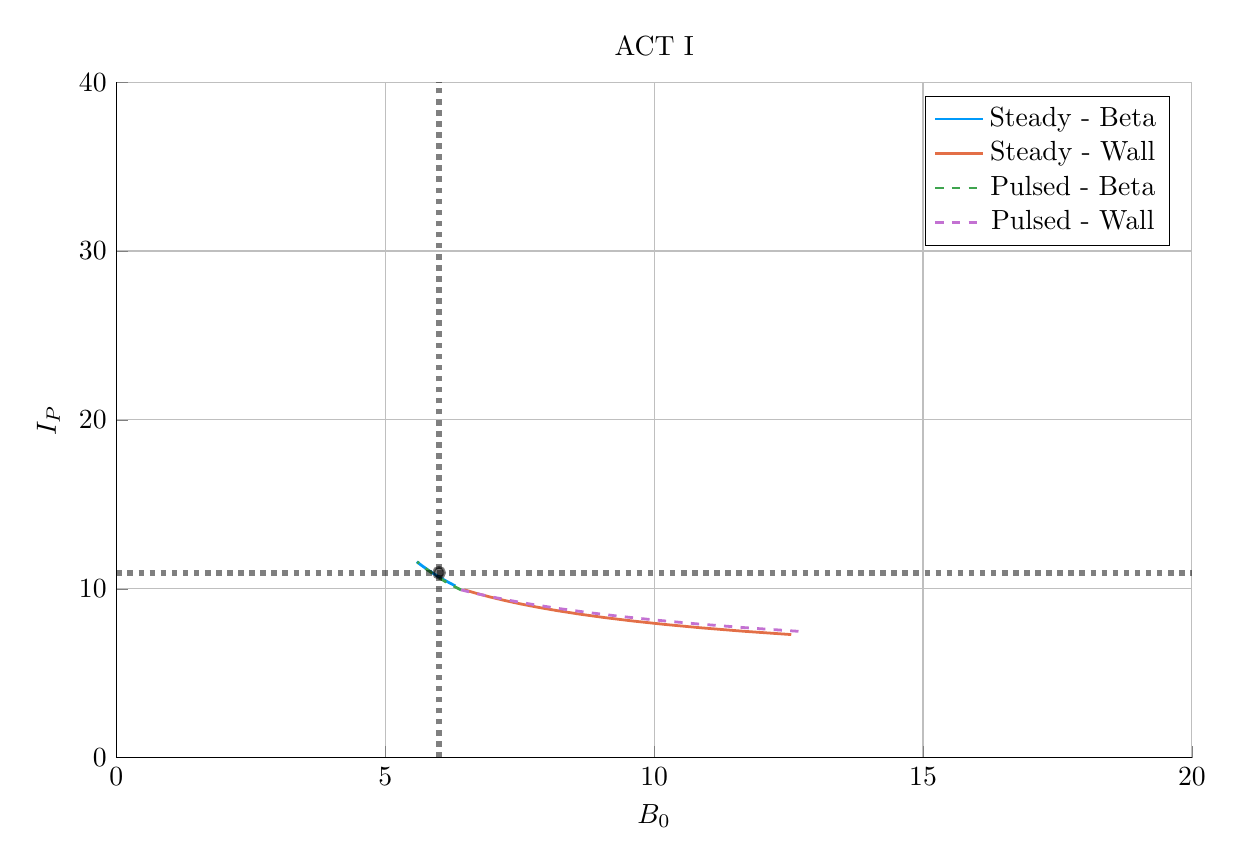
\begin{tikzpicture}[]
\begin{axis}[height = {101.6mm}, ylabel = {${I}_{P}$}, title = {ACT I}, xmin = {0.0}, xmax = {20.0}, ymax = {40.0}, xlabel = {${B}_{0}$}, {unbounded coords=jump, scaled x ticks = false, xticklabel style={rotate = 0}, xmajorgrids = true, xtick = {0.0,5.0,10.0,15.0,20.0}, xticklabels = {0,5,10,15,20}, xtick align = inside, axis lines* = left, scaled y ticks = false, yticklabel style={rotate = 0}, ymajorgrids = true, ytick = {0.0,10.0,20.0,30.0,40.0}, yticklabels = {0,10,20,30,40}, ytick align = inside, axis lines* = left,     xshift = 0.0mm,
    yshift = 0.0mm,
    axis background/.style={fill={rgb,1:red,1.00000000;green,1.00000000;blue,1.00000000}}
, colorbar style={title=}}, ymin = {0.0}, width = {152.4mm}]\addplot+ [color = {rgb,1:red,0.00000000;green,0.60560316;blue,0.97868012},
draw opacity=1.0,
line width=1,
solid,mark = none,
mark size = 2.0,
mark options = {
    color = {rgb,1:red,0.00000000;green,0.00000000;blue,0.00000000}, draw opacity = 1.0,
    fill = {rgb,1:red,0.00000000;green,0.60560316;blue,0.97868012}, fill opacity = 1.0,
    line width = 1,
    rotate = 0,
    solid
}]coordinates {
(6.30336807958207, 10.169194435531358)
(6.162193069273141, 10.405057509328124)
(6.030717178404645, 10.641905327194731)
(5.908065509576601, 10.87971637136811)
(5.793464904530972, 11.11846917050157)
(5.686229631357383, 11.358142407296011)
(5.585749511271037, 11.598714938197329)
};
\addlegendentry{Steady - Beta}
\addplot+ [color = {rgb,1:red,0.88887350;green,0.43564919;blue,0.27812294},
draw opacity=1.0,
line width=1,
solid,mark = none,
mark size = 2.0,
mark options = {
    color = {rgb,1:red,0.00000000;green,0.00000000;blue,0.00000000}, draw opacity = 1.0,
    fill = {rgb,1:red,0.88887350;green,0.43564919;blue,0.27812294}, fill opacity = 1.0,
    line width = 1,
    rotate = 0,
    solid
}]coordinates {
(12.549536249695134, 7.287903136887)
(11.658754653696462, 7.486025430610099)
(10.883719833507003, 7.685696663157812)
(10.206258129789394, 7.886645361110723)
(9.611335769312953, 8.08866940687473)
(9.086446934250878, 8.291629426976055)
(8.62129895070743, 8.495414075666067)
(8.207216040989662, 8.699964056113311)
(7.837119555085499, 8.905213556979005)
(7.505047858717157, 9.111120468746519)
(7.20604322925957, 9.31764336053339)
(6.935884710193303, 9.524758318501357)
(6.691016583192173, 9.732442959434447)
(6.468415485086983, 9.940679052729761)
};
\addlegendentry{Steady - Wall}
\addplot+ [color = {rgb,1:red,0.24222430;green,0.64327509;blue,0.30444865},
draw opacity=1.0,
line width=1,
dashed,mark = none,
mark size = 2.0,
mark options = {
    color = {rgb,1:red,0.00000000;green,0.00000000;blue,0.00000000}, draw opacity = 1.0,
    fill = {rgb,1:red,0.24222430;green,0.64327509;blue,0.30444865}, fill opacity = 1.0,
    line width = 1,
    rotate = 0,
    solid
}]coordinates {
(6.408263337806559, 9.933500150990564)
(6.408263337806564, 9.933500150990564)
(6.385466513301022, 9.969282740147014)
(6.245492502072912, 10.199548426407084)
(6.116010320461132, 10.430379144484162)
(5.9960421481916395, 10.661750348679098)
(5.884727159112828, 10.893638132753678)
(5.781304768121868, 11.126019229767902)
(5.685100648450046, 11.358871009413285)
(5.595515000321003, 11.592171473618816)
};
\addlegendentry{Pulsed - Beta}
\addplot+ [color = {rgb,1:red,0.76444018;green,0.44411178;blue,0.82429754},
draw opacity=1.0,
line width=1,
dashed,mark = none,
mark size = 2.0,
mark options = {
    color = {rgb,1:red,0.00000000;green,0.00000000;blue,0.00000000}, draw opacity = 1.0,
    fill = {rgb,1:red,0.76444018;green,0.44411178;blue,0.82429754}, fill opacity = 1.0,
    line width = 1,
    rotate = 0,
    solid
}]coordinates {
(12.684248532650473, 7.481290856821823)
(11.66307871570063, 7.703549290655078)
(10.781888309639141, 7.92668121689452)
(10.016282491385791, 8.15065615613957)
(9.346943280276514, 8.375443966327172)
(8.758420158941194, 8.601014900773066)
(8.238241792953433, 8.82733966430566)
(7.776255600865612, 9.054389459546684)
(7.364131118520045, 9.282136024328327)
(6.994982564641668, 9.510551661584085)
(6.66307916140573, 9.73960926266661)
(6.408263337806559, 9.933500150990564)
(6.408263337806564, 9.933500150990564)
};
\addlegendentry{Pulsed - Wall}
\addplot+ [color = {rgb,1:red,0.00000000;green,0.00000000;blue,0.00000000},
draw opacity=0.5,
line width=2,
dotted,mark = none,
mark size = 2.0,
mark options = {
    color = {rgb,1:red,0.00000000;green,0.00000000;blue,0.00000000}, draw opacity = 0.5,
    fill = {rgb,1:red,0.00000000;green,0.00000000;blue,0.00000000}, fill opacity = 0.5,
    line width = 1,
    rotate = 0,
    solid
},forget plot]coordinates {
(0.0, 10.95)
(20.0, 10.95)
};
\addplot+ [color = {rgb,1:red,0.00000000;green,0.00000000;blue,0.00000000},
draw opacity=0.5,
line width=2,
dotted,mark = none,
mark size = 2.0,
mark options = {
    color = {rgb,1:red,0.00000000;green,0.00000000;blue,0.00000000}, draw opacity = 0.5,
    fill = {rgb,1:red,0.00000000;green,0.00000000;blue,0.00000000}, fill opacity = 0.5,
    line width = 1,
    rotate = 0,
    solid
},forget plot]coordinates {
(6.0, 0.0)
(6.0, 40.0)
};
\addplot+[draw=none, color = {rgb,1:red,0.00000000;green,0.00000000;blue,0.00000000},
draw opacity=0.5,
line width=0,
solid,mark = *,
mark size = 2.0,
mark options = {
    color = {rgb,1:red,0.00000000;green,0.00000000;blue,0.00000000}, draw opacity = 0.5,
    fill = {rgb,1:red,0.00000000;green,0.00000000;blue,0.00000000}, fill opacity = 0.5,
    line width = 1,
    rotate = 0,
    solid
},forget plot] coordinates {
(6.0, 10.95)
};
\end{axis}

\end{tikzpicture}

    \end{adjustbox}
        \caption{ACT I}
    \end{subfigure}
    \hfill
    \begin{subfigure}[t]{0.45\textwidth}
        \centering
    \begin{adjustbox}{width=\textwidth}
      \Large
      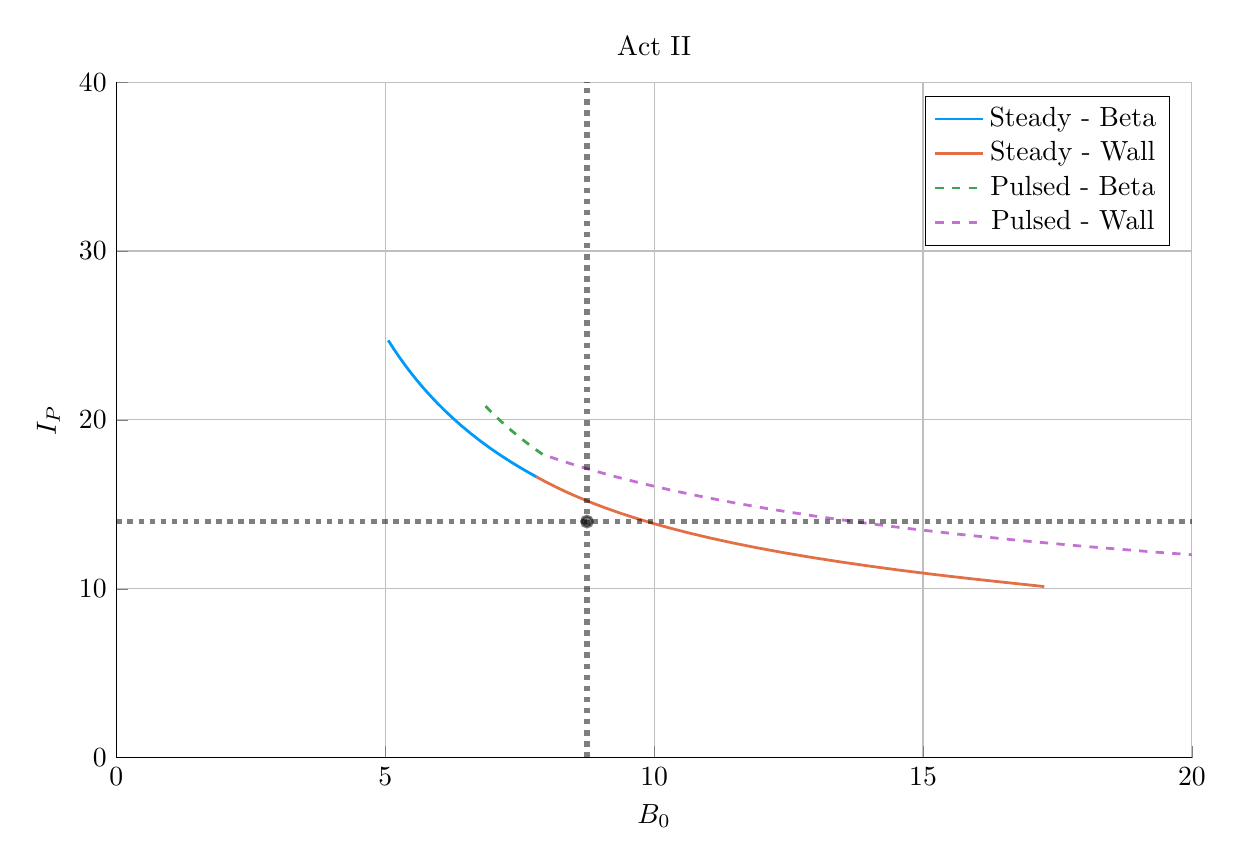
\begin{tikzpicture}[]
\begin{axis}[height = {101.6mm}, ylabel = {${I}_{P}$}, title = {Act II}, xmin = {0.0}, xmax = {20.0}, ymax = {40.0}, xlabel = {${B}_{0}$}, {unbounded coords=jump, scaled x ticks = false, xticklabel style={rotate = 0}, xmajorgrids = true, xtick = {0.0,5.0,10.0,15.0,20.0}, xticklabels = {0,5,10,15,20}, xtick align = inside, axis lines* = left, scaled y ticks = false, yticklabel style={rotate = 0}, ymajorgrids = true, ytick = {0.0,10.0,20.0,30.0,40.0}, yticklabels = {0,10,20,30,40}, ytick align = inside, axis lines* = left,     xshift = 0.0mm,
    yshift = 0.0mm,
    axis background/.style={fill={rgb,1:red,1.00000000;green,1.00000000;blue,1.00000000}}
, colorbar style={title=}}, ymin = {0.0}, width = {152.4mm}]\addplot+ [color = {rgb,1:red,0.00000000;green,0.60560316;blue,0.97868012},
draw opacity=1.0,
line width=1,
solid,mark = none,
mark size = 2.0,
mark options = {
    color = {rgb,1:red,0.00000000;green,0.00000000;blue,0.00000000}, draw opacity = 1.0,
    fill = {rgb,1:red,0.00000000;green,0.60560316;blue,0.97868012}, fill opacity = 1.0,
    line width = 1,
    rotate = 0,
    solid
}]coordinates {
(7.810935944285959, 16.626976584120992)
(7.57736049850867, 17.04714126565062)
(7.354864292609041, 17.4728205159228)
(7.145167234136329, 17.902037802268676)
(6.9473303865083675, 18.334710756318135)
(6.760499508614096, 18.770758343299946)
(6.583897990324067, 19.21009903030823)
(6.416817229618043, 19.652652028291016)
(6.258609820663305, 20.098337062332053)
(6.108683264880386, 20.547074418426956)
(5.966494431410919, 20.998784986741654)
(5.831544666176381, 21.453390301179443)
(5.703375459679132, 21.910812577709113)
(5.581564609582325, 22.37097474604109)
(5.465722802994068, 22.833800482195542)
(5.355490573482678, 23.299214237115898)
(5.25053558682053, 23.767141260842724)
(5.1505502068221745, 24.237507628970306)
(5.0552493196883175, 24.710240262329886)
};
\addlegendentry{Steady - Beta}
\addplot+ [color = {rgb,1:red,0.88887350;green,0.43564919;blue,0.27812294},
draw opacity=1.0,
line width=1,
solid,mark = none,
mark size = 2.0,
mark options = {
    color = {rgb,1:red,0.00000000;green,0.00000000;blue,0.00000000}, draw opacity = 1.0,
    fill = {rgb,1:red,0.88887350;green,0.43564919;blue,0.27812294}, fill opacity = 1.0,
    line width = 1,
    rotate = 0,
    solid
}]coordinates {
(17.25550839059296, 10.131702672149428)
(16.594334962335296, 10.354462623384137)
(15.9071755430688, 10.591104956642406)
(15.233983138507648, 10.837356598740662)
(14.594239858921854, 11.09054386610192)
(13.989673082630297, 11.349883742416331)
(13.414782495717416, 11.61561327802365)
(12.872659546281994, 11.886764241828663)
(12.364365715508608, 12.16256217004895)
(11.889507953196574, 12.44240841774136)
(11.44685939646348, 12.72583049098312)
(11.034739998180656, 13.012449288635679)
(10.651252523287319, 13.301956539143166)
(10.294428800132035, 13.59409872387861)
(9.962319203963213, 13.888665310111481)
(9.653045819449929, 14.185479949266789)
(9.364832254395445, 14.48439377498311)
(9.096018465506306, 14.785280223642218)
(8.844373144802077, 15.088238807947413)
(8.61055754360846, 15.392552774473998)
(8.391192178573277, 15.698764813772398)
(8.18577947665566, 16.00659672680533)
(7.99323348423048, 16.315986303185774)
(7.812301489248497, 16.626976584120992)
};
\addlegendentry{Steady - Wall}
\addplot+ [color = {rgb,1:red,0.24222430;green,0.64327509;blue,0.30444865},
draw opacity=1.0,
line width=1,
dashed,mark = none,
mark size = 2.0,
mark options = {
    color = {rgb,1:red,0.00000000;green,0.00000000;blue,0.00000000}, draw opacity = 1.0,
    fill = {rgb,1:red,0.24222430;green,0.64327509;blue,0.30444865}, fill opacity = 1.0,
    line width = 1,
    rotate = 0,
    solid
}]coordinates {
(7.923668284887995, 17.96627417153032)
(7.923668284887995, 17.966274171530337)
(7.836759696043437, 18.1591936305205)
(7.6662731560983355, 18.555297107283753)
(7.50499428233835, 18.953426399022014)
(7.35232773269976, 19.353497539767794)
(7.207727224738343, 19.7554274455778)
(7.070690693175276, 20.159133974954596)
(6.940756001029682, 20.564535986760628)
(6.817497143644154, 20.971553389451927)
};
\addlegendentry{Pulsed - Beta}
\addplot+ [color = {rgb,1:red,0.76444018;green,0.44411178;blue,0.82429754},
draw opacity=1.0,
line width=1,
dashed,mark = none,
mark size = 2.0,
mark options = {
    color = {rgb,1:red,0.00000000;green,0.00000000;blue,0.00000000}, draw opacity = 1.0,
    fill = {rgb,1:red,0.76444018;green,0.44411178;blue,0.82429754}, fill opacity = 1.0,
    line width = 1,
    rotate = 0,
    solid
}]coordinates {
(22.56106430311702, 11.474678053719876)
(20.85607192394036, 11.819475032994422)
(19.335265246056654, 12.167858357397087)
(17.974121547130903, 12.51974460671026)
(16.751976718553127, 12.875049128346197)
(15.651329744019142, 13.233686175102404)
(14.65728744097675, 13.595569077154208)
(13.757118584462601, 13.96061040317257)
(12.939893642194303, 14.328722110173729)
(12.196191964860315, 14.699815683529526)
(11.517862472405039, 15.073802268415148)
(10.897827027335556, 15.450592793824576)
(10.329918077124672, 15.830098089115069)
(9.808743940706389, 16.21222899561205)
(9.329576544487265, 16.596896471191773)
(8.888257451278507, 16.984011690059134)
(8.481118883411932, 17.37348613728185)
(8.10491708701527, 17.765231698435688)
(7.923668284887995, 17.96627417153032)
(7.923668284887995, 17.966274171530337)
};
\addlegendentry{Pulsed - Wall}
\addplot+ [color = {rgb,1:red,0.00000000;green,0.00000000;blue,0.00000000},
draw opacity=0.5,
line width=2,
dotted,mark = none,
mark size = 2.0,
mark options = {
    color = {rgb,1:red,0.00000000;green,0.00000000;blue,0.00000000}, draw opacity = 0.5,
    fill = {rgb,1:red,0.00000000;green,0.00000000;blue,0.00000000}, fill opacity = 0.5,
    line width = 1,
    rotate = 0,
    solid
},forget plot]coordinates {
(0.0, 13.98)
(20.0, 13.98)
};
\addplot+ [color = {rgb,1:red,0.00000000;green,0.00000000;blue,0.00000000},
draw opacity=0.5,
line width=2,
dotted,mark = none,
mark size = 2.0,
mark options = {
    color = {rgb,1:red,0.00000000;green,0.00000000;blue,0.00000000}, draw opacity = 0.5,
    fill = {rgb,1:red,0.00000000;green,0.00000000;blue,0.00000000}, fill opacity = 0.5,
    line width = 1,
    rotate = 0,
    solid
},forget plot]coordinates {
(8.75, 0.0)
(8.75, 40.0)
};
\addplot+[draw=none, color = {rgb,1:red,0.00000000;green,0.00000000;blue,0.00000000},
draw opacity=0.5,
line width=0,
solid,mark = *,
mark size = 2.0,
mark options = {
    color = {rgb,1:red,0.00000000;green,0.00000000;blue,0.00000000}, draw opacity = 0.5,
    fill = {rgb,1:red,0.00000000;green,0.00000000;blue,0.00000000}, fill opacity = 0.5,
    line width = 1,
    rotate = 0,
    solid
},forget plot] coordinates {
(8.75, 13.98)
};
\end{axis}

\end{tikzpicture}

    \end{adjustbox}
        \caption{ACT II}
    \end{subfigure}
    \hfill \hfill ~\\ ~\\ ~\\ ~\\
  \caption[]{Magnet Scan: $I_P$ vs $B_0$} ~\\
\end{figure*}


\clearpage

\newpage

\subsection*{ Major Radius -- $R_0$ }
  \label{subsection:scan_R_0}

\begin{figure*}[h!]
    \centering
    \hfill
    \begin{subfigure}[t]{0.45\textwidth}
        \centering
    \begin{adjustbox}{width=\textwidth}
      \Large
      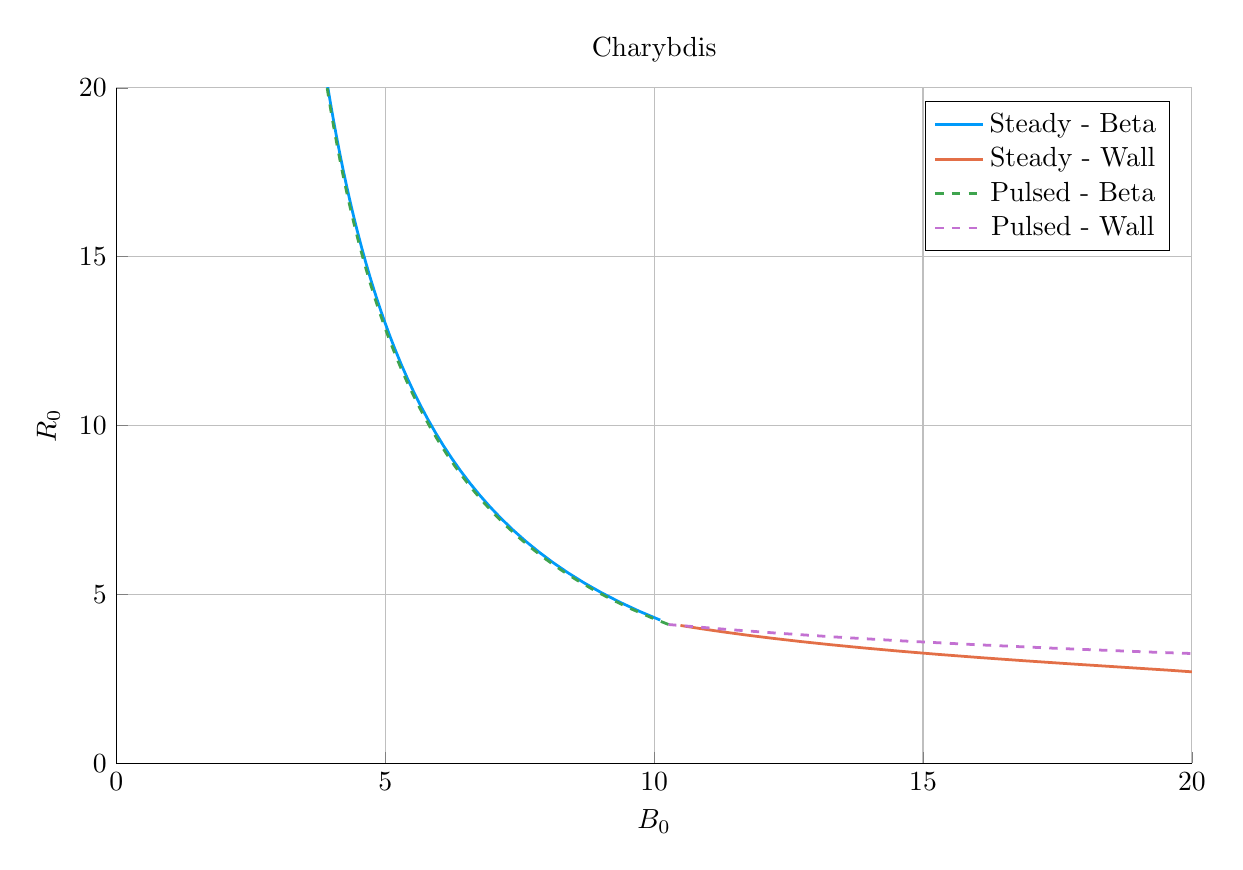
\begin{tikzpicture}[]
\begin{axis}[height = {101.6mm}, ylabel = {${R}_{0}$}, title = {Charybdis}, xmin = {0.0}, xmax = {20.0}, ymax = {20.0}, xlabel = {${B}_{0}$}, {unbounded coords=jump, scaled x ticks = false, xticklabel style={rotate = 0}, xmajorgrids = true, xtick = {0.0,5.0,10.0,15.0,20.0}, xticklabels = {0,5,10,15,20}, xtick align = inside, axis lines* = left, scaled y ticks = false, yticklabel style={rotate = 0}, ymajorgrids = true, ytick = {0.0,5.0,10.0,15.0,20.0}, yticklabels = {0,5,10,15,20}, ytick align = inside, axis lines* = left,     xshift = 0.0mm,
    yshift = 0.0mm,
    axis background/.style={fill={rgb,1:red,1.00000000;green,1.00000000;blue,1.00000000}}
, colorbar style={title=}}, ymin = {0.0}, width = {152.4mm}]\addplot+ [color = {rgb,1:red,0.00000000;green,0.60560316;blue,0.97868012},
draw opacity=1.0,
line width=1,
solid,mark = none,
mark size = 2.0,
mark options = {
    color = {rgb,1:red,0.00000000;green,0.00000000;blue,0.00000000}, draw opacity = 1.0,
    fill = {rgb,1:red,0.00000000;green,0.60560316;blue,0.97868012}, fill opacity = 1.0,
    line width = 1,
    rotate = 0,
    solid
}]coordinates {
(10.112818033153026, 4.241771689478311)
(9.722156888543116, 4.504138117525138)
(9.357875603858393, 4.77497367032698)
(9.017653755630063, 5.054228410858618)
(8.6995124437054, 5.34178832481448)
(8.401566530516865, 5.637594610921002)
(8.122163706328223, 5.941556970897918)
(7.859819415455661, 6.2535750482800845)
(7.613196557650265, 6.5735387749268055)
(7.381088038653343, 6.901328733442317)
(7.162401716104116, 7.236816533350192)
(6.956147367527331, 7.579865198961832)
(6.761425371986388, 7.930329566972662)
(6.577416849463348, 8.28805669191591)
(6.403375044688587, 8.652886257700402)
(6.2386177769852695, 9.02465099355178)
(6.0825208065966905, 9.403177092267818)
(5.934511989185341, 9.788284632344096)
(5.794066116682695, 10.179787994954152)
(5.660700347012839, 10.577496284633074)
(5.533970150598111, 10.981213744847159)
(5.413465705416883, 11.390740170754555)
(5.298808685607224, 11.805871315185586)
(5.189649392059402, 12.226399293085946)
(5.085664187259174, 12.652112975136994)
(4.986553195072601, 13.082798376170517)
(4.892038235455667, 13.518239035062717)
(4.801860966679364, 13.958216385902286)
(4.7157812114040425, 14.402510119861804)
(4.633575445956479, 14.850898537267405)
(4.5550354347559185, 15.303158889428241)
(4.479966994069385, 15.759067709846747)
(4.408188871204256, 16.21840113449116)
(4.33953172691477, 16.680935210866018)
(4.273837210246432, 17.14644619566822)
(4.210957116299974, 17.614710840865197)
(4.15075261849161, 18.085506668079862)
(4.0930935678432965, 18.558612231207235)
(4.037857852672517, 19.03380736722975)
(3.9849308127842145, 19.510873435234036)
(3.9342047029103653, 19.98959354366903)
(3.8855782007091695, 20.46975276591405)
(3.838955955133626, 20.951138344257103)
(3.7942481714200484, 21.433539882408354)
(3.7513702293348077, 21.91674952670236)
(3.710242331663442, 22.400562136158193)
(3.6707891802306123, 22.88477544159215)
(3.6329396770109583, 23.369190193993973)
(3.5966266481325166, 23.853610302391182)
(3.5617865887889004, 24.33784296144382)
(3.5283594272686503, 24.821698769019683)
(3.496288306480746, 25.30499183401733)
(3.465519381509793, 25.787539874702443)
(3.4360016318699595, 26.2691643078435)
(3.4076866872513096, 26.74969032892794)
(3.380528665662031, 27.228946983749)
(3.3544840229690007, 27.706767231660894)
(3.3295114129297314, 28.18298800079238)
(3.3055715568879336, 28.6574502355218)
(3.2826271223788512, 29.129998936506894)
(3.260642607548369, 29.600483215419466)
(3.239584247604666, 30.068756211731234)
(3.2194198921826622, 30.53467533068977)
(3.2001189373344725, 30.998102038032528)
(3.181652227422265, 31.45890197647381)
(3.163991977015565, 31.916944945395528)
(3.1471116955378684, 32.37210489697581)
(3.130986116696265, 32.82425992717794)
(3.115591132350856, 33.27329226186858)
(3.1009037305081053, 33.719088238329654)
(3.0869019371473265, 34.16153828242195)
(3.0735647616124355, 34.600536881650775)
(3.0608721453218655, 35.035982554380354)
};
\addlegendentry{Steady - Beta}
\addplot+ [color = {rgb,1:red,0.88887350;green,0.43564919;blue,0.27812294},
draw opacity=1.0,
line width=1,
solid,mark = none,
mark size = 2.0,
mark options = {
    color = {rgb,1:red,0.00000000;green,0.00000000;blue,0.00000000}, draw opacity = 1.0,
    fill = {rgb,1:red,0.88887350;green,0.43564919;blue,0.27812294}, fill opacity = 1.0,
    line width = 1,
    rotate = 0,
    solid
}]coordinates {
(20.758867641064707, 2.5885674971573294)
(20.346250098246923, 2.6701608818805265)
(19.57104597888471, 2.7580768645580767)
(18.681781921115476, 2.84914579801761)
(17.775790175980152, 2.942053074257325)
(16.896654716492492, 3.036102404206255)
(16.063927450323227, 3.1308756359103893)
(15.285557510665852, 3.226095678435203)
(14.563500533069154, 3.3215674678202314)
(13.896568848875791, 3.417147967307318)
(13.281970890030232, 3.5127292434426214)
(12.716170469467318, 3.6082281475654683)
(12.195372283741088, 3.7035796419955296)
(11.715794270833433, 3.798732281084355)
(11.273815669498969, 3.8936450383948094)
(10.866051794088186, 3.9882850129983627)
(10.489365023931143, 4.08262666943062)
};
\addlegendentry{Steady - Wall}
\addplot+ [color = {rgb,1:red,0.24222430;green,0.64327509;blue,0.30444865},
draw opacity=1.0,
line width=1,
dashed,mark = none,
mark size = 2.0,
mark options = {
    color = {rgb,1:red,0.00000000;green,0.00000000;blue,0.00000000}, draw opacity = 1.0,
    fill = {rgb,1:red,0.24222430;green,0.64327509;blue,0.30444865}, fill opacity = 1.0,
    line width = 1,
    rotate = 0,
    solid
}]coordinates {
(10.26788634689966, 4.1112515557786775)
(9.953967652326213, 4.3094639978912825)
(9.567926244368271, 4.576742787082168)
(9.207974394987358, 4.852707848855866)
(8.871841888699304, 5.137296446755483)
(8.557505525932248, 5.430432251844937)
(8.263156925406376, 5.732025498645217)
(7.9871752024348766, 6.041973183885721)
(7.728103682045175, 6.3601593098028015)
(7.484629973620137, 6.686455168691173)
(7.255568856523303, 7.020719666856628)
(7.039847526735421, 7.362799685753208)
(6.836492834698909, 7.712530477959993)
(6.644620209081183, 8.06973609553486)
(6.463424013335149, 8.43422984818008)
(6.2921691243175495, 8.80581478856818)
(6.13018355681404, 9.184284222105854)
(5.97685198655569, 9.569422237740964)
(5.831610044919842, 9.961004260702955)
(5.693939286027163, 10.358797615092055)
(5.563362729090489, 10.762562105803609)
(5.439440906144732, 11.172050607751359)
(5.321768347746793, 11.587009663771289)
(5.209970453003084, 12.007180084871303)
(5.103700692769835, 12.43229755779498)
(5.002638109938164, 12.862093246958203)
(4.906485077678376, 13.296294396161224)
(4.814965286571576, 13.734624924501638)
(4.727821933804548, 14.176806014771396)
(4.644816091323922, 14.622556692215932)
(4.565725232806084, 15.071594391671503)
(4.490341901840154, 15.523635511246878)
(4.418472505906755, 15.978395950871612)
(4.349936222622964, 16.435591634187325)
(4.284564006352339, 16.89493901242702)
(4.222197684694192, 17.3561555490841)
(4.162689135592264, 17.818960184341037)
(4.105899536872315, 18.283073778386605)
(4.051698680949713, 18.748219532911282)
(3.9999643482627323, 19.214123390225897)
(3.9505817337017928, 19.680514409594025)
(3.903442920928527, 20.147125120523665)
(3.858446400032002, 20.613691852887264)
(3.8154966244515616, 21.079955043879853)
(3.7745036035252744, 21.545659521938795)
(3.7353825273991994, 22.010554767868463)
(3.6980534213689746, 22.47439515350876)
(3.6624408270205375, 22.936940158387063)
(3.62847350780097, 23.397954564874027)
(3.5960841768845415, 23.85720863243935)
(3.565209245407392, 24.314478251672824)
(3.5357885893311605, 24.769545078785413)
(3.5077653333614305, 25.22219665136009)
(3.4810856504959875, 25.672226486155235)
(3.4556985759109375, 26.119434159797105)
(3.4315558340122845, 26.563625373217942)
(3.408611677587535, 27.004612000714285)
(3.3868227380888998, 27.44221212450356)
(3.36614788616562, 27.876250055664674)
(3.3465481016421226, 28.306556342336567)
(3.327986352208224, 28.732967766047434)
(3.3104274769652595, 29.155327355093103)
(3.2938380965241474, 29.573484219331384)
(3.278186482171801, 29.987293796610192)
(3.263442495132517, 30.396617529277517)
(3.2495774839156075, 30.801322953869263)
(3.236564206241785, 31.2012836153002)
(3.224376752844934, 31.596379002720997)
(3.212990475972638, 31.98649447963656)
(3.2023819222517877, 32.371521208907616)
(3.192528769611062, 32.751356073231776)
(3.1834097679780142, 33.12590159165121)
(3.1750046834890777, 33.49506583261046)
(3.1672942459724482, 33.8587623240416)
};
\addlegendentry{Pulsed - Beta}
\addplot+ [color = {rgb,1:red,0.76444018;green,0.44411178;blue,0.82429754},
draw opacity=1.0,
line width=1,
dashed,mark = none,
mark size = 2.0,
mark options = {
    color = {rgb,1:red,0.00000000;green,0.00000000;blue,0.00000000}, draw opacity = 1.0,
    fill = {rgb,1:red,0.76444018;green,0.44411178;blue,0.82429754}, fill opacity = 1.0,
    line width = 1,
    rotate = 0,
    solid
}]coordinates {
(48.990476413653056, 2.408463256282958)
(42.83950920694117, 2.5157944044289065)
(37.687790427214495, 2.623911121514849)
(33.33937742845888, 2.732773154793489)
(29.64296398154308, 2.8423415573543895)
(26.48039367255613, 2.9525785265823425)
(23.758442882319894, 3.0634472709719978)
(21.402860298405816, 3.174911900538905)
(19.353987387634486, 3.2869373368800954)
(17.563502020363714, 3.3994892396762393)
(15.991970371213752, 3.512533946790301)
(14.606987499719377, 3.6260384258753686)
(13.381751501116137, 3.7399702354868722)
(12.293960329570087, 3.854297494171075)
(11.32495111804522, 3.9689888562032056)
(10.459023415380802, 4.084013492866982)
(10.26788634689966, 4.1112515557786775)
};
\addlegendentry{Pulsed - Wall}
\end{axis}

\end{tikzpicture}

    \end{adjustbox}
        \caption{Charybdis}
    \end{subfigure}
    \hfill
    \begin{subfigure}[t]{0.45\textwidth}
        \centering
    \begin{adjustbox}{width=\textwidth}
      \Large
      \begin{tikzpicture}[]
\begin{axis}[height = {101.6mm}, ylabel = {${R}_{0}$}, title = {Proteus}, xmin = {0.0}, xmax = {20.0}, ymax = {20.0}, xlabel = {${B}_{0}$}, {unbounded coords=jump, scaled x ticks = false, xticklabel style={rotate = 0}, xmajorgrids = true, xtick = {0.0,5.0,10.0,15.0,20.0}, xticklabels = {0,5,10,15,20}, xtick align = inside, axis lines* = left, scaled y ticks = false, yticklabel style={rotate = 0}, ymajorgrids = true, ytick = {0.0,5.0,10.0,15.0,20.0}, yticklabels = {0,5,10,15,20}, ytick align = inside, axis lines* = left,     xshift = 0.0mm,
    yshift = 0.0mm,
    axis background/.style={fill={rgb,1:red,1.00000000;green,1.00000000;blue,1.00000000}}
, colorbar style={title=}}, ymin = {0.0}, width = {152.4mm}]\addplot+ [color = {rgb,1:red,0.00000000;green,0.60560316;blue,0.97868012},
draw opacity=1.0,
line width=1,
solid,mark = none,
mark size = 2.0,
mark options = {
    color = {rgb,1:red,0.00000000;green,0.00000000;blue,0.00000000}, draw opacity = 1.0,
    fill = {rgb,1:red,0.00000000;green,0.60560316;blue,0.97868012}, fill opacity = 1.0,
    line width = 1,
    rotate = 0,
    solid
}]coordinates {
(4.658732060637907, 15.19267920719026)
(4.211109766361548, 13.257359890602805)
(3.9293920326356777, 11.874737313931622)
(3.7651903683456465, 10.866007699416029)
(3.6776039543745567, 10.103021459180615)
(3.6402437753208394, 9.505760636119051)
(3.6366994671255806, 9.024418756735512)
(3.656621534643579, 8.627122931627166)
(3.693300156736026, 8.29276379316033)
(3.7422515017241134, 8.006879676976913)
(3.865532743079537, 7.5424484228595015)
(3.936096932264377, 7.350942552250971)
(4.010907188015084, 7.180521653028847)
(4.089072356933184, 7.027918062531758)
(4.169903401491354, 6.8905526178616)
(4.252857906625248, 6.7663586425757165)
(4.337501757261618, 6.653657691692545)
(4.42348218754058, 6.551070097987566)
(4.5983381267510195, 6.371833566535418)
(4.686766232902671, 6.29340795554276)
(4.775618142770625, 6.221477142908907)
(4.864743502376605, 6.155442914152805)
(4.927312314219091, 6.1123879686673135)
};
\addlegendentry{Pulsed - Kink}
\addplot+ [color = {rgb,1:red,0.88887350;green,0.43564919;blue,0.27812294},
draw opacity=1.0,
line width=1,
solid,mark = none,
mark size = 2.0,
mark options = {
    color = {rgb,1:red,0.00000000;green,0.00000000;blue,0.00000000}, draw opacity = 1.0,
    fill = {rgb,1:red,0.88887350;green,0.43564919;blue,0.27812294}, fill opacity = 1.0,
    line width = 1,
    rotate = 0,
    solid
}]coordinates {
(4.927312314219091, 6.1123879686673135)
(4.984545814413324, 6.09581207033949)
(5.17452482724068, 6.0447147858623)
(5.362091669637646, 5.999934523234248)
(5.54700293215903, 5.961033646850443)
(5.729042482638278, 5.92761240871646)
(5.908022832274664, 5.899302777254819)
(6.083785777786694, 5.87576371038825)
(6.256202341425288, 5.85667756374391)
(6.324169421042356, 5.850226299362774)
};
\addlegendentry{Pulsed - Beta}
\addplot+ [color = {rgb,1:red,0.24222430;green,0.64327509;blue,0.30444865},
draw opacity=1.0,
line width=1,
solid,mark = none,
mark size = 2.0,
mark options = {
    color = {rgb,1:red,0.00000000;green,0.00000000;blue,0.00000000}, draw opacity = 1.0,
    fill = {rgb,1:red,0.24222430;green,0.64327509;blue,0.30444865}, fill opacity = 1.0,
    line width = 1,
    rotate = 0,
    solid
}]coordinates {
(6.324169421042356, 5.850226299362774)
(6.727338549778396, 5.88388315153579)
(7.320469048424473, 5.950696360836003)
(7.835746509376305, 6.026778469060774)
(8.290245520072391, 6.109137751468495)
(8.696162676727877, 6.195913809142839)
(9.0624397222742, 6.285887257774413)
(9.395798186463841, 6.3782240354403505)
(9.701405747258567, 6.472333393687546)
(10.244760202900984, 6.664256338261126)
(10.930275827723788, 6.957604003970967)
(11.131878682735255, 7.056189303396245)
(11.50278450645086, 7.253945523825199)
(11.83715172742864, 7.452031096358636)
(11.992609772603878, 7.551070724623068)
(12.141110720831467, 7.650057379146056)
};
\addlegendentry{Pulsed - Wall}
\end{axis}

\end{tikzpicture}

    \end{adjustbox}
        \caption{Proteus}
    \end{subfigure}
    \hfill \hfill ~\\ ~\\ ~\\ ~\\
    \hfill
    \begin{subfigure}[t]{0.45\textwidth}
        \centering
    \begin{adjustbox}{width=\textwidth}
      \Large
      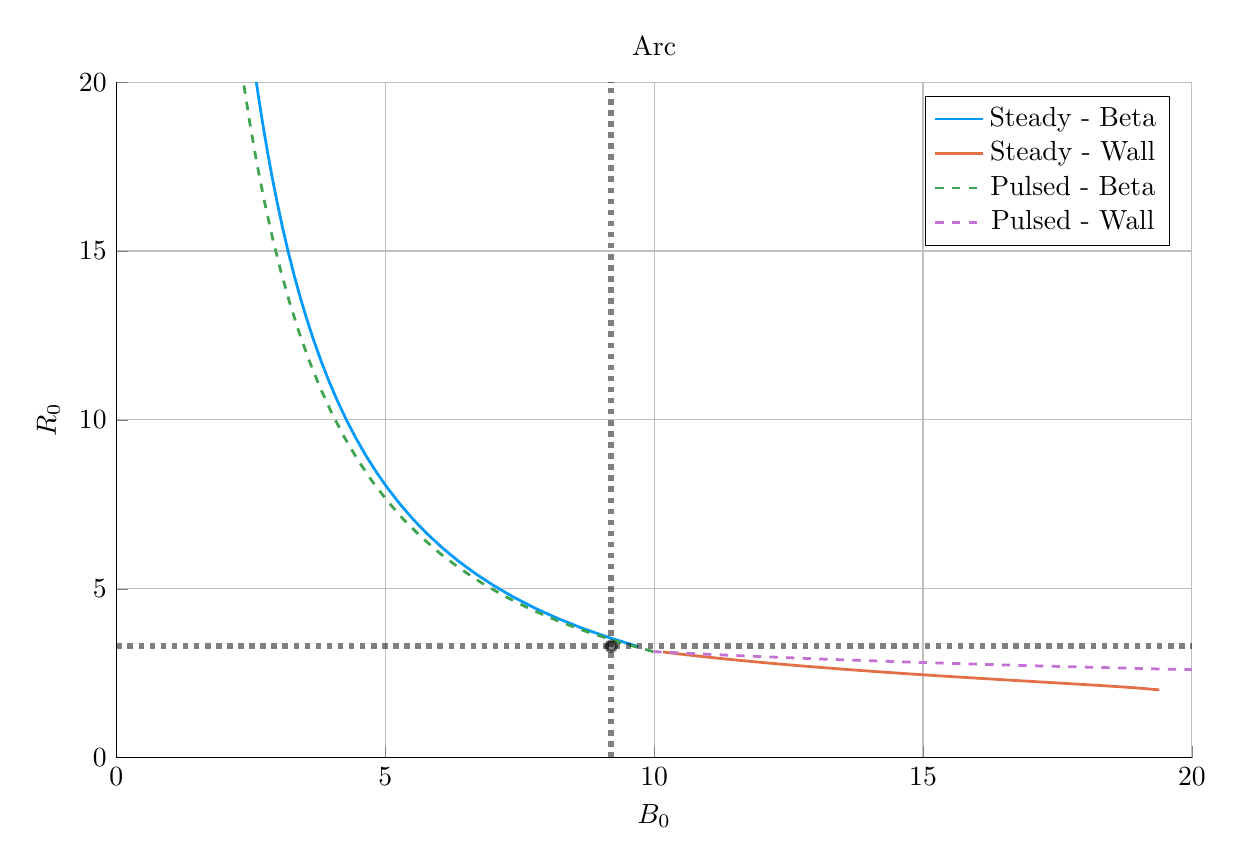
\begin{tikzpicture}[]
\begin{axis}[height = {101.6mm}, ylabel = {${R}_{0}$}, title = {Arc}, xmin = {0.0}, xmax = {20.0}, ymax = {20.0}, xlabel = {${B}_{0}$}, {unbounded coords=jump, scaled x ticks = false, xticklabel style={rotate = 0}, xmajorgrids = true, xtick = {0.0,5.0,10.0,15.0,20.0}, xticklabels = {0,5,10,15,20}, xtick align = inside, axis lines* = left, scaled y ticks = false, yticklabel style={rotate = 0}, ymajorgrids = true, ytick = {0.0,5.0,10.0,15.0,20.0}, yticklabels = {0,5,10,15,20}, ytick align = inside, axis lines* = left,     xshift = 0.0mm,
    yshift = 0.0mm,
    axis background/.style={fill={rgb,1:red,1.00000000;green,1.00000000;blue,1.00000000}}
, colorbar style={title=}}, ymin = {0.0}, width = {152.4mm}]\addplot+ [color = {rgb,1:red,0.00000000;green,0.60560316;blue,0.97868012},
draw opacity=1.0,
line width=1,
solid,mark = none,
mark size = 2.0,
mark options = {
    color = {rgb,1:red,0.00000000;green,0.00000000;blue,0.00000000}, draw opacity = 1.0,
    fill = {rgb,1:red,0.00000000;green,0.60560316;blue,0.97868012}, fill opacity = 1.0,
    line width = 1,
    rotate = 0,
    solid
}]coordinates {
(9.701206080853105, 3.2904233285656006)
(9.162315904693079, 3.553631706046861)
(8.664301107137337, 3.8315748016260343)
(8.203576462497304, 4.124583886864978)
(7.776718537485166, 4.433072975674755)
(7.380720231870917, 4.75741949036414)
(7.012886014999712, 5.097987291342331)
(6.670795005901889, 5.4551257000070565)
(6.352268997292712, 5.829168567645448)
(6.055344682097163, 6.220433393277178)
(5.778249464564785, 6.629220493040615)
(5.519380338856715, 7.05581222339423)
(5.2772854007125325, 7.500472260074458)
(5.050647625972996, 7.963444934423652)
(4.838270606140816, 8.444954628380609)
(4.639065978019038, 8.94520522910952)
(4.4520423235376105, 9.464379643936518)
(4.276295348572609, 10.002639375969222)
(4.110999177018484, 10.56012416048812)
(3.9553986195015125, 11.136951661929974)
(3.8088022956698633, 11.733217231026282)
(3.6705765055641186, 12.34899372141899)
(3.54013975965751, 12.984331364849716)
(3.4169578891619192, 13.639257703809928)
(3.30053966845824, 14.313777580345645)
(3.1904328903033052, 15.007873179535935)
(3.086220842019516, 15.721504126002731)
(2.9875191373772063, 16.45460763166718)
(2.8939728644914635, 17.207098692842226)
(2.8052540149097247, 17.97887033463821)
(2.7210591632720242, 18.7697939005645)
(2.6411073705789065, 19.579719385129263)
(2.565138287279709, 20.40847580717446)
(2.492910435164382, 21.255871621630877)
(2.4241996494611984, 22.12169516733927)
(2.3587976646588236, 23.0057151485579)
(2.296510829425685, 23.907681147764652)
(2.237158937627476, 24.827324167354146)
(2.180574163874242, 25.764357197843207)
(2.126600093288366, 26.71847581021091)
(2.075090836295778, 27.689358770027713)
(2.0259102202234582, 28.676668671060817)
(1.978931050353818, 29.68005258608471)
(1.9340344338545452, 30.69914273267572)
(1.8911091606836798, 31.733557151818793)
(1.8500511361739687, 32.78290039722107)
(1.8107628605384507, 33.846764233283025)
(1.773152951016952, 34.92472833975579)
(1.7371357028100902, 36.01636102117257)
(1.7026306853269466, 37.121219919229354)
(1.6695623706125668, 38.23885272635799)
(1.6378597911249178, 39.368797898817405)
(1.607456224302725, 40.51058536770822)
(1.5782889016090462, 41.663737246396295)
(1.5502987399539199, 42.82776853291479)
(1.5234300935954943, 44.00218780599217)
(1.4976305247952577, 45.18649791343829)
(1.4728505916614916, 46.38019665170201)
(1.4490436517578602, 47.58277743549339)
(1.4261656801829077, 48.79372995643627)
};
\addlegendentry{Steady - Beta}
\addplot+ [color = {rgb,1:red,0.88887350;green,0.43564919;blue,0.27812294},
draw opacity=1.0,
line width=1,
solid,mark = none,
mark size = 2.0,
mark options = {
    color = {rgb,1:red,0.00000000;green,0.00000000;blue,0.00000000}, draw opacity = 1.0,
    fill = {rgb,1:red,0.88887350;green,0.43564919;blue,0.27812294}, fill opacity = 1.0,
    line width = 1,
    rotate = 0,
    solid
}]coordinates {
(19.394007482712425, 2.006855814841082)
(18.932196567189358, 2.070220226465634)
(18.296989378345195, 2.1362327099649083)
(17.587029315408756, 2.2039322514902886)
(16.847882407994106, 2.272885741349308)
(16.111374502564406, 2.3427307443133163)
(15.396027314547156, 2.4132115621474344)
(14.710952688793137, 2.484165095168367)
(14.06168447794857, 2.555449485048069)
(13.450465418483889, 2.6269568263788754)
(12.877644538645335, 2.6986005527245354)
(12.342394470642008, 2.7703103261458715)
(11.843182246608265, 2.8420284550528074)
(11.376441269625893, 2.9137564749008216)
(10.944966372727551, 2.985307257194073)
(10.541663878705513, 3.056795384934831)
(10.165908182236457, 3.128148092221394)
};
\addlegendentry{Steady - Wall}
\addplot+ [color = {rgb,1:red,0.24222430;green,0.64327509;blue,0.30444865},
draw opacity=1.0,
line width=1,
dashed,mark = none,
mark size = 2.0,
mark options = {
    color = {rgb,1:red,0.00000000;green,0.00000000;blue,0.00000000}, draw opacity = 1.0,
    fill = {rgb,1:red,0.24222430;green,0.64327509;blue,0.30444865}, fill opacity = 1.0,
    line width = 1,
    rotate = 0,
    solid
}]coordinates {
(9.980483622051658, 3.1402982942956537)
(9.392786903460065, 3.3984668375583613)
(8.79273598103983, 3.7029994270206985)
(8.23820290909994, 4.029752381934837)
(7.725182218401588, 4.380005330007902)
(7.250078106370205, 4.755088191072525)
(6.80965553466646, 5.15638156809462)
(6.400998063035608, 5.585317075247801)
(6.0214713600430425, 6.043377623224966)
(5.668691517461799, 6.532097691007738)
(5.340497445229901, 7.053063624618788)
(5.034926745580058, 7.607914017422467)
(4.750194564008521, 8.198340243900201)
(4.484674995755211, 8.826087240213646)
(4.236884692979903, 9.49295465115087)
(4.00546837264544, 10.200798495308337)
(3.7891859704718387, 10.951533539957822)
(3.5869012239550364, 11.747136625739826)
(3.3975714987448393, 12.589651241396528)
(3.2202386987489797, 13.481193723261853)
(3.0540211220494466, 14.423961547290066)
(2.8981061427709687, 15.420244298711943)
(2.7517436139566023, 16.472438053930638)
(2.6142398986781377, 17.58306410230943)
(2.4849524463010138, 18.754793188384546)
(2.363284838174807, 19.990476791576892)
(2.248682232019848, 21.293187416028662)
(2.140627136740878, 22.666270490916787)
(2.038635448877246, 24.113411362836906)
(1.9422526775794744, 25.638722123308433)
(1.8510502754751532, 27.246854857488287)
(1.7646219756564088, 28.94315065234289)
(1.6825800061969869, 30.73383791051506)
(1.6045510059627948, 32.62630011975996)
(1.53017138625397, 34.629443897654504)
(1.4590817483192686, 36.754215952550474)
(1.3909197311384796, 39.01434852880224)
(1.3253102336217724, 41.42746903285954)
(1.261851128383913, 44.01681696754988)
(1.20009089049112, 46.81403058684408)
(1.1394908096975784, 49.863950342519615)
};
\addlegendentry{Pulsed - Beta}
\addplot+ [color = {rgb,1:red,0.76444018;green,0.44411178;blue,0.82429754},
draw opacity=1.0,
line width=1,
dashed,mark = none,
mark size = 2.0,
mark options = {
    color = {rgb,1:red,0.00000000;green,0.00000000;blue,0.00000000}, draw opacity = 1.0,
    fill = {rgb,1:red,0.76444018;green,0.44411178;blue,0.82429754}, fill opacity = 1.0,
    line width = 1,
    rotate = 0,
    solid
}]coordinates {
(29.27715761652869, 2.3448804182939873)
(25.4410619834368, 2.4377937236066716)
(22.158819835998365, 2.5322208586485804)
(19.342453256965573, 2.628163744265164)
(16.919364280634177, 2.7256238396687067)
(14.829378672669455, 2.8246020951898183)
(13.022412368922526, 2.9250989082568273)
(11.456617692058645, 3.0271140820266207)
(10.096901921254785, 3.1306467862637533)
(9.980483622051658, 3.1402982942956537)
};
\addlegendentry{Pulsed - Wall}
\addplot+ [color = {rgb,1:red,0.00000000;green,0.00000000;blue,0.00000000},
draw opacity=0.5,
line width=2,
dotted,mark = none,
mark size = 2.0,
mark options = {
    color = {rgb,1:red,0.00000000;green,0.00000000;blue,0.00000000}, draw opacity = 0.5,
    fill = {rgb,1:red,0.00000000;green,0.00000000;blue,0.00000000}, fill opacity = 0.5,
    line width = 1,
    rotate = 0,
    solid
},forget plot]coordinates {
(0.0, 3.3)
(20.0, 3.3)
};
\addplot+ [color = {rgb,1:red,0.00000000;green,0.00000000;blue,0.00000000},
draw opacity=0.5,
line width=2,
dotted,mark = none,
mark size = 2.0,
mark options = {
    color = {rgb,1:red,0.00000000;green,0.00000000;blue,0.00000000}, draw opacity = 0.5,
    fill = {rgb,1:red,0.00000000;green,0.00000000;blue,0.00000000}, fill opacity = 0.5,
    line width = 1,
    rotate = 0,
    solid
},forget plot]coordinates {
(9.2, 0.0)
(9.2, 20.0)
};
\addplot+[draw=none, color = {rgb,1:red,0.00000000;green,0.00000000;blue,0.00000000},
draw opacity=0.5,
line width=0,
solid,mark = *,
mark size = 2.0,
mark options = {
    color = {rgb,1:red,0.00000000;green,0.00000000;blue,0.00000000}, draw opacity = 0.5,
    fill = {rgb,1:red,0.00000000;green,0.00000000;blue,0.00000000}, fill opacity = 0.5,
    line width = 1,
    rotate = 0,
    solid
},forget plot] coordinates {
(9.2, 3.3)
};
\end{axis}

\end{tikzpicture}

    \end{adjustbox}
        \caption{ARC}
    \end{subfigure}
    \hfill
    \begin{subfigure}[t]{0.45\textwidth}
        \centering
    \begin{adjustbox}{width=\textwidth}
      \Large
      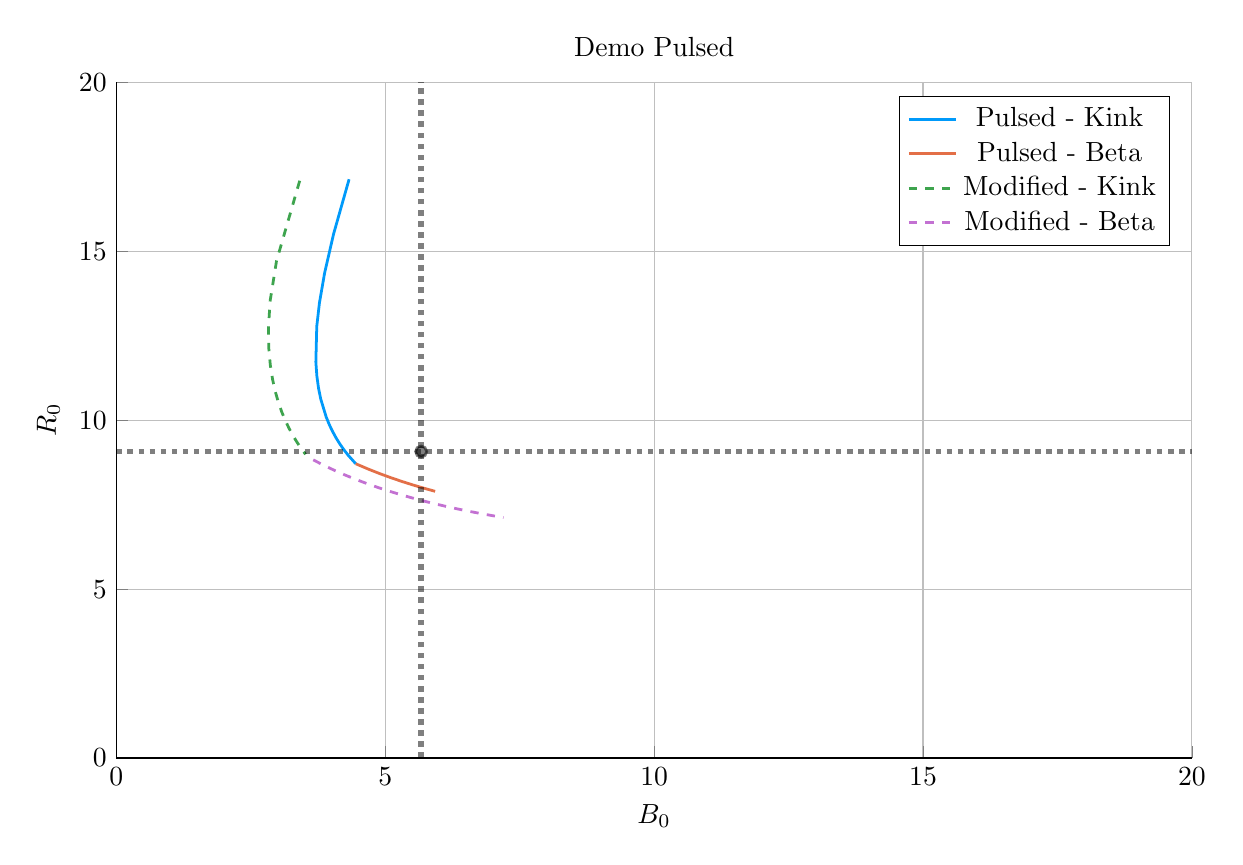
\begin{tikzpicture}[]
\begin{axis}[height = {101.6mm}, ylabel = {${R}_{0}$}, title = {Demo Pulsed}, xmin = {0.0}, xmax = {20.0}, ymax = {20.0}, xlabel = {${B}_{0}$}, {unbounded coords=jump, scaled x ticks = false, xticklabel style={rotate = 0}, xmajorgrids = true, xtick = {0.0,5.0,10.0,15.0,20.0}, xticklabels = {0,5,10,15,20}, xtick align = inside, axis lines* = left, scaled y ticks = false, yticklabel style={rotate = 0}, ymajorgrids = true, ytick = {0.0,5.0,10.0,15.0,20.0}, yticklabels = {0,5,10,15,20}, ytick align = inside, axis lines* = left,     xshift = 0.0mm,
    yshift = 0.0mm,
    axis background/.style={fill={rgb,1:red,1.00000000;green,1.00000000;blue,1.00000000}}
, colorbar style={title=}}, ymin = {0.0}, width = {152.4mm}]\addplot+ [color = {rgb,1:red,0.00000000;green,0.60560316;blue,0.97868012},
draw opacity=1.0,
line width=1,
solid,mark = none,
mark size = 2.0,
mark options = {
    color = {rgb,1:red,0.00000000;green,0.00000000;blue,0.00000000}, draw opacity = 1.0,
    fill = {rgb,1:red,0.00000000;green,0.60560316;blue,0.97868012}, fill opacity = 1.0,
    line width = 1,
    rotate = 0,
    solid
}]coordinates {
(4.327031075670194, 17.134796748649162)
(4.038214026054326, 15.511755022601415)
(3.8713719163129245, 14.355562963913712)
(3.7758613845615545, 13.476675762289453)
(3.7257856761317214, 12.778294295391971)
(3.7090473695925437, 11.723065749829066)
(3.727711597554826, 11.30970201784727)
(3.7586131667481433, 10.94971275897184)
(3.799052518631718, 10.632190690377048)
(3.901290136389271, 10.09455415135144)
(3.960577465316514, 9.863813619410237)
(4.0241209645210345, 9.653307397969705)
(4.0912717805663785, 9.460162902699798)
(4.161514602943343, 9.28206292757184)
(4.2344343960723005, 9.117114543572253)
(4.309692554546368, 8.963753917462126)
(4.450417240491067, 8.712493965092264)
};
\addlegendentry{Pulsed - Kink}
\addplot+ [color = {rgb,1:red,0.88887350;green,0.43564919;blue,0.27812294},
draw opacity=1.0,
line width=1,
solid,mark = none,
mark size = 2.0,
mark options = {
    color = {rgb,1:red,0.00000000;green,0.00000000;blue,0.00000000}, draw opacity = 1.0,
    fill = {rgb,1:red,0.88887350;green,0.43564919;blue,0.27812294}, fill opacity = 1.0,
    line width = 1,
    rotate = 0,
    solid
}]coordinates {
(4.450417240491067, 8.712493965092264)
(4.490148631384312, 8.684308742646298)
(4.692490181445514, 8.547262773806349)
(4.8960344619053355, 8.41947837460442)
(5.100651132702229, 8.30014929484307)
(5.306202822090688, 8.188581738801314)
(5.512545696627038, 8.084175191078112)
(5.719530043226767, 7.986407002697611)
(5.927000883375481, 7.894819882619234)
};
\addlegendentry{Pulsed - Beta}
\addplot+ [color = {rgb,1:red,0.24222430;green,0.64327509;blue,0.30444865},
draw opacity=1.0,
line width=1,
dashed,mark = none,
mark size = 2.0,
mark options = {
    color = {rgb,1:red,0.00000000;green,0.00000000;blue,0.00000000}, draw opacity = 1.0,
    fill = {rgb,1:red,0.24222430;green,0.64327509;blue,0.30444865}, fill opacity = 1.0,
    line width = 1,
    rotate = 0,
    solid
}]coordinates {
(3.4087424183072135, 17.090884129081292)
(2.977074181068944, 14.713048632784332)
(2.8592500074202523, 13.541171522519205)
(2.827199220063259, 12.740024138753894)
(2.8339789008667826, 12.12574468151967)
(2.862412302880871, 11.626187613249266)
(2.9044598258085443, 11.205091848948229)
(2.95577893007882, 10.841432203317366)
(3.0137895352525907, 10.521822649209419)
(3.076849710218805, 10.23716073884787)
(3.1438583711612704, 9.980947801083442)
(3.214045733980633, 9.748367275345563)
(3.2868548955983727, 9.535742205343247)
(3.361871149981842, 9.340197658526863)
(3.4387778750377818, 9.15944098345979)
(3.5173279629378453, 8.991613349767409)
};
\addlegendentry{Modified - Kink}
\addplot+ [color = {rgb,1:red,0.76444018;green,0.44411178;blue,0.82429754},
draw opacity=1.0,
line width=1,
dashed,mark = none,
mark size = 2.0,
mark options = {
    color = {rgb,1:red,0.00000000;green,0.00000000;blue,0.00000000}, draw opacity = 1.0,
    fill = {rgb,1:red,0.76444018;green,0.44411178;blue,0.82429754}, fill opacity = 1.0,
    line width = 1,
    rotate = 0,
    solid
}]coordinates {
(3.6607028750648505, 8.825949645171955)
(3.8574448036470477, 8.664618827122876)
(4.056375867871351, 8.51434867582932)
(4.257366397480293, 8.374075613831488)
(4.460279103534801, 8.242896218794312)
(4.664969389370631, 8.12003771613466)
(4.871285596007394, 8.004834914067093)
(5.07906923307514, 7.896711937521184)
(5.288155233306219, 7.795167587687744)
(5.498372259673351, 7.699763475973523)
(5.709543087166185, 7.610114306522102)
(5.921485076209294, 7.525879840414137)
(6.134010749367255, 7.446758190646709)
(6.346928478632384, 7.372480180910637)
(6.560043285872518, 7.302804563889649)
(6.773157754368795, 7.237513941672651)
(6.986073044284746, 7.176411266758267)
(7.198590001107076, 7.119316828230052)
};
\addlegendentry{Modified - Beta}
\addplot+ [color = {rgb,1:red,0.00000000;green,0.00000000;blue,0.00000000},
draw opacity=0.5,
line width=2,
dotted,mark = none,
mark size = 2.0,
mark options = {
    color = {rgb,1:red,0.00000000;green,0.00000000;blue,0.00000000}, draw opacity = 0.5,
    fill = {rgb,1:red,0.00000000;green,0.00000000;blue,0.00000000}, fill opacity = 0.5,
    line width = 1,
    rotate = 0,
    solid
},forget plot]coordinates {
(0.0, 9.072)
(20.0, 9.072)
};
\addplot+ [color = {rgb,1:red,0.00000000;green,0.00000000;blue,0.00000000},
draw opacity=0.5,
line width=2,
dotted,mark = none,
mark size = 2.0,
mark options = {
    color = {rgb,1:red,0.00000000;green,0.00000000;blue,0.00000000}, draw opacity = 0.5,
    fill = {rgb,1:red,0.00000000;green,0.00000000;blue,0.00000000}, fill opacity = 0.5,
    line width = 1,
    rotate = 0,
    solid
},forget plot]coordinates {
(5.667, 0.0)
(5.667, 20.0)
};
\addplot+[draw=none, color = {rgb,1:red,0.00000000;green,0.00000000;blue,0.00000000},
draw opacity=0.5,
line width=0,
solid,mark = *,
mark size = 2.0,
mark options = {
    color = {rgb,1:red,0.00000000;green,0.00000000;blue,0.00000000}, draw opacity = 0.5,
    fill = {rgb,1:red,0.00000000;green,0.00000000;blue,0.00000000}, fill opacity = 0.5,
    line width = 1,
    rotate = 0,
    solid
},forget plot] coordinates {
(5.667, 9.072)
};
\end{axis}

\end{tikzpicture}

    \end{adjustbox}
        \caption{DEMO Pulsed}
    \end{subfigure}
    \hfill \hfill ~\\ ~\\ ~\\ ~\\
    \hfill
    \begin{subfigure}[t]{0.45\textwidth}
        \centering
    \begin{adjustbox}{width=\textwidth}
      \Large
      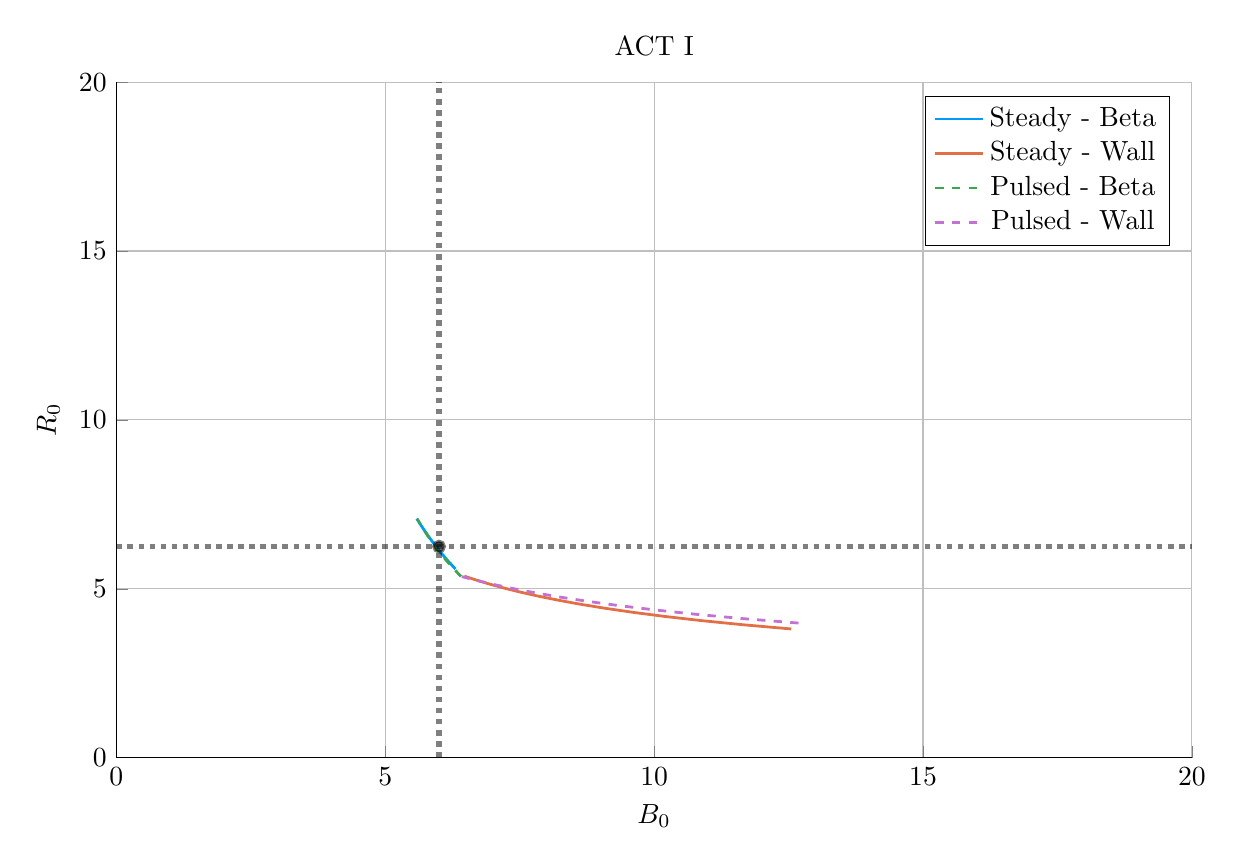
\begin{tikzpicture}[]
\begin{axis}[height = {101.6mm}, ylabel = {${R}_{0}$}, title = {ACT I}, xmin = {0.0}, xmax = {20.0}, ymax = {20.0}, xlabel = {${B}_{0}$}, {unbounded coords=jump, scaled x ticks = false, xticklabel style={rotate = 0}, xmajorgrids = true, xtick = {0.0,5.0,10.0,15.0,20.0}, xticklabels = {0,5,10,15,20}, xtick align = inside, axis lines* = left, scaled y ticks = false, yticklabel style={rotate = 0}, ymajorgrids = true, ytick = {0.0,5.0,10.0,15.0,20.0}, yticklabels = {0,5,10,15,20}, ytick align = inside, axis lines* = left,     xshift = 0.0mm,
    yshift = 0.0mm,
    axis background/.style={fill={rgb,1:red,1.00000000;green,1.00000000;blue,1.00000000}}
, colorbar style={title=}}, ymin = {0.0}, width = {152.4mm}]\addplot+ [color = {rgb,1:red,0.00000000;green,0.60560316;blue,0.97868012},
draw opacity=1.0,
line width=1,
solid,mark = none,
mark size = 2.0,
mark options = {
    color = {rgb,1:red,0.00000000;green,0.00000000;blue,0.00000000}, draw opacity = 1.0,
    fill = {rgb,1:red,0.00000000;green,0.60560316;blue,0.97868012}, fill opacity = 1.0,
    line width = 1,
    rotate = 0,
    solid
}]coordinates {
(6.30336807958207, 5.587199391496101)
(6.162193069273141, 5.831838137107903)
(6.030717178404645, 6.078157823726375)
(5.908065509576601, 6.325994353145188)
(5.793464904530972, 6.57518910191267)
(5.686229631357383, 6.825588847053452)
(5.585749511271037, 7.077045564754442)
};
\addlegendentry{Steady - Beta}
\addplot+ [color = {rgb,1:red,0.88887350;green,0.43564919;blue,0.27812294},
draw opacity=1.0,
line width=1,
solid,mark = none,
mark size = 2.0,
mark options = {
    color = {rgb,1:red,0.00000000;green,0.00000000;blue,0.00000000}, draw opacity = 1.0,
    fill = {rgb,1:red,0.88887350;green,0.43564919;blue,0.27812294}, fill opacity = 1.0,
    line width = 1,
    rotate = 0,
    solid
}]coordinates {
(12.549536249695134, 3.8108352245940957)
(11.658754653696462, 3.934083270736017)
(10.883719833507003, 4.057046546594516)
(10.206258129789394, 4.179626810883221)
(9.611335769312953, 4.301750356443285)
(9.086446934250878, 4.423366229113912)
(8.62129895070743, 4.544434218016914)
(8.207216040989662, 4.6649335402400025)
(7.837119555085499, 4.78484200403474)
(7.505047858717157, 4.9041467319817595)
(7.20604322925957, 5.022835870779136)
(6.935884710193303, 5.1409045607718795)
(6.691016583192173, 5.258349129805506)
(6.468415485086983, 5.375167957409874)
};
\addlegendentry{Steady - Wall}
\addplot+ [color = {rgb,1:red,0.24222430;green,0.64327509;blue,0.30444865},
draw opacity=1.0,
line width=1,
dashed,mark = none,
mark size = 2.0,
mark options = {
    color = {rgb,1:red,0.00000000;green,0.00000000;blue,0.00000000}, draw opacity = 1.0,
    fill = {rgb,1:red,0.24222430;green,0.64327509;blue,0.30444865}, fill opacity = 1.0,
    line width = 1,
    rotate = 0,
    solid
}]coordinates {
(6.408263337806559, 5.366131328829866)
(6.408263337806564, 5.366131328829862)
(6.385466513301022, 5.402805883604879)
(6.245492502072912, 5.638974714472524)
(6.116010320461132, 5.875875066688821)
(5.9960421481916395, 6.113307727774442)
(5.884727159112828, 6.351082733498888)
(5.781304768121868, 6.589019058920955)
(5.685100648450046, 6.826944315253105)
(5.595515000321003, 7.064694456596427)
};
\addlegendentry{Pulsed - Beta}
\addplot+ [color = {rgb,1:red,0.76444018;green,0.44411178;blue,0.82429754},
draw opacity=1.0,
line width=1,
dashed,mark = none,
mark size = 2.0,
mark options = {
    color = {rgb,1:red,0.00000000;green,0.00000000;blue,0.00000000}, draw opacity = 1.0,
    fill = {rgb,1:red,0.76444018;green,0.44411178;blue,0.82429754}, fill opacity = 1.0,
    line width = 1,
    rotate = 0,
    solid
}]coordinates {
(12.684248532650473, 3.9847907768802657)
(11.66307871570063, 4.114684512780648)
(10.781888309639141, 4.244124103742294)
(10.016282491385791, 4.373086052625054)
(9.346943280276514, 4.501549309887817)
(8.758420158941194, 4.6294950281779785)
(8.238241792953433, 4.756906348757686)
(7.776255600865612, 4.883768212546736)
(7.364131118520045, 5.010067192354689)
(6.994982564641668, 5.135791343697217)
(6.66307916140573, 5.260930071474144)
(6.408263337806559, 5.366131328829866)
(6.408263337806564, 5.366131328829862)
};
\addlegendentry{Pulsed - Wall}
\addplot+ [color = {rgb,1:red,0.00000000;green,0.00000000;blue,0.00000000},
draw opacity=0.5,
line width=2,
dotted,mark = none,
mark size = 2.0,
mark options = {
    color = {rgb,1:red,0.00000000;green,0.00000000;blue,0.00000000}, draw opacity = 0.5,
    fill = {rgb,1:red,0.00000000;green,0.00000000;blue,0.00000000}, fill opacity = 0.5,
    line width = 1,
    rotate = 0,
    solid
},forget plot]coordinates {
(0.0, 6.25)
(20.0, 6.25)
};
\addplot+ [color = {rgb,1:red,0.00000000;green,0.00000000;blue,0.00000000},
draw opacity=0.5,
line width=2,
dotted,mark = none,
mark size = 2.0,
mark options = {
    color = {rgb,1:red,0.00000000;green,0.00000000;blue,0.00000000}, draw opacity = 0.5,
    fill = {rgb,1:red,0.00000000;green,0.00000000;blue,0.00000000}, fill opacity = 0.5,
    line width = 1,
    rotate = 0,
    solid
},forget plot]coordinates {
(6.0, 0.0)
(6.0, 20.0)
};
\addplot+[draw=none, color = {rgb,1:red,0.00000000;green,0.00000000;blue,0.00000000},
draw opacity=0.5,
line width=0,
solid,mark = *,
mark size = 2.0,
mark options = {
    color = {rgb,1:red,0.00000000;green,0.00000000;blue,0.00000000}, draw opacity = 0.5,
    fill = {rgb,1:red,0.00000000;green,0.00000000;blue,0.00000000}, fill opacity = 0.5,
    line width = 1,
    rotate = 0,
    solid
},forget plot] coordinates {
(6.0, 6.25)
};
\end{axis}

\end{tikzpicture}

    \end{adjustbox}
        \caption{ACT I}
    \end{subfigure}
    \hfill
    \begin{subfigure}[t]{0.45\textwidth}
        \centering
    \begin{adjustbox}{width=\textwidth}
      \Large
      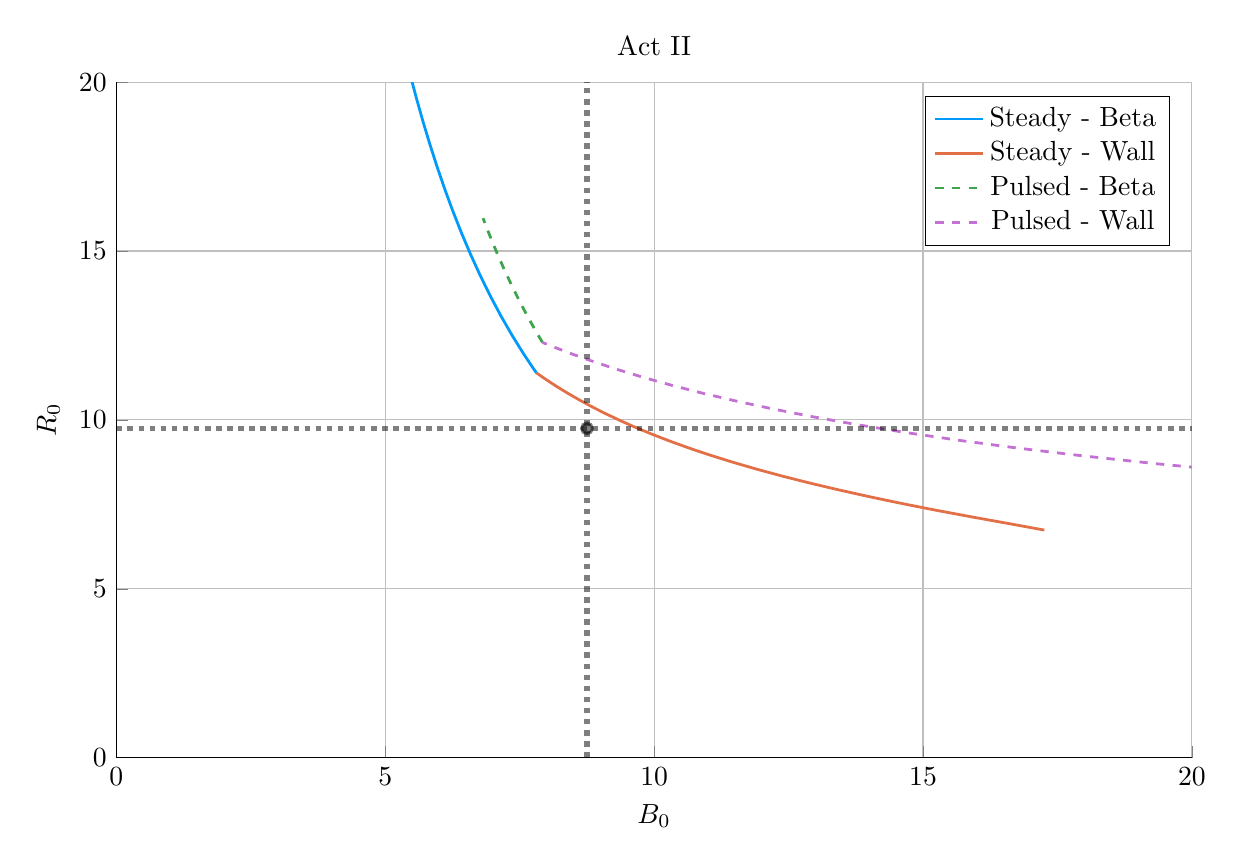
\begin{tikzpicture}[]
\begin{axis}[height = {101.6mm}, ylabel = {${R}_{0}$}, title = {Act II}, xmin = {0.0}, xmax = {20.0}, ymax = {20.0}, xlabel = {${B}_{0}$}, {unbounded coords=jump, scaled x ticks = false, xticklabel style={rotate = 0}, xmajorgrids = true, xtick = {0.0,5.0,10.0,15.0,20.0}, xticklabels = {0,5,10,15,20}, xtick align = inside, axis lines* = left, scaled y ticks = false, yticklabel style={rotate = 0}, ymajorgrids = true, ytick = {0.0,5.0,10.0,15.0,20.0}, yticklabels = {0,5,10,15,20}, ytick align = inside, axis lines* = left,     xshift = 0.0mm,
    yshift = 0.0mm,
    axis background/.style={fill={rgb,1:red,1.00000000;green,1.00000000;blue,1.00000000}}
, colorbar style={title=}}, ymin = {0.0}, width = {152.4mm}]\addplot+ [color = {rgb,1:red,0.00000000;green,0.60560316;blue,0.97868012},
draw opacity=1.0,
line width=1,
solid,mark = none,
mark size = 2.0,
mark options = {
    color = {rgb,1:red,0.00000000;green,0.00000000;blue,0.00000000}, draw opacity = 1.0,
    fill = {rgb,1:red,0.00000000;green,0.60560316;blue,0.97868012}, fill opacity = 1.0,
    line width = 1,
    rotate = 0,
    solid
}]coordinates {
(7.810935944285959, 11.389141268081966)
(7.57736049850867, 11.942634046586162)
(7.354864292609041, 12.51245847357923)
(7.145167234136329, 13.0943365692581)
(6.9473303865083675, 13.687993788149779)
(6.760499508614096, 14.293145886478186)
(6.583897990324067, 14.909495325365516)
(6.416817229618043, 15.536734694045393)
(6.258609820663305, 16.1745467994937)
(6.108683264880386, 16.82260538899235)
(5.966494431410919, 17.480575868750975)
(5.831544666176381, 18.148116014600475)
(5.703375459679132, 18.824876684423757)
(5.581564609582325, 19.510502502077443)
(5.465722802994068, 20.20463254880097)
(5.355490573482678, 20.906901035327614)
(5.25053558682053, 21.616937949657327)
(5.1505502068221745, 22.334369714080776)
(5.0552493196883175, 23.058819802110854)
};
\addlegendentry{Steady - Beta}
\addplot+ [color = {rgb,1:red,0.88887350;green,0.43564919;blue,0.27812294},
draw opacity=1.0,
line width=1,
solid,mark = none,
mark size = 2.0,
mark options = {
    color = {rgb,1:red,0.00000000;green,0.00000000;blue,0.00000000}, draw opacity = 1.0,
    fill = {rgb,1:red,0.88887350;green,0.43564919;blue,0.27812294}, fill opacity = 1.0,
    line width = 1,
    rotate = 0,
    solid
}]coordinates {
(17.25550839059296, 6.738604635617289)
(16.594334962335296, 6.931178286222189)
(15.9071755430688, 7.128187388035985)
(15.233983138507648, 7.327817939330552)
(14.594239858921854, 7.528927553154291)
(13.989673082630297, 7.7312042898700515)
(13.414782495717416, 7.934790159202381)
(12.872659546281994, 8.139273115071695)
(12.364365715508608, 8.344321605506495)
(11.889507953196574, 8.549679244077495)
(11.44685939646348, 8.755144058838903)
(11.034739998180656, 8.960554762148757)
(10.651252523287319, 9.165781242855727)
(10.294428800132035, 9.370717743724994)
(9.962319203963213, 9.57527782549947)
(9.653045819449929, 9.779390564591205)
(9.364832254395445, 9.982997628553138)
(9.096018465506306, 10.186050992034668)
(8.844373144802077, 10.388606525997883)
(8.61055754360846, 10.590345571972314)
(8.391192178573277, 10.791527736428888)
(8.18577947665566, 10.992035979756642)
(7.99323348423048, 11.1918525509058)
(7.812301489248497, 11.391007917726574)
};
\addlegendentry{Steady - Wall}
\addplot+ [color = {rgb,1:red,0.24222430;green,0.64327509;blue,0.30444865},
draw opacity=1.0,
line width=1,
dashed,mark = none,
mark size = 2.0,
mark options = {
    color = {rgb,1:red,0.00000000;green,0.00000000;blue,0.00000000}, draw opacity = 1.0,
    fill = {rgb,1:red,0.24222430;green,0.64327509;blue,0.30444865}, fill opacity = 1.0,
    line width = 1,
    rotate = 0,
    solid
}]coordinates {
(7.923668284887995, 12.293879059492616)
(7.923668284887995, 12.293879059492635)
(7.836759696043437, 12.52591633746021)
(7.6662731560983355, 13.00454403942661)
(7.50499428233835, 13.488375025456907)
(7.35232773269976, 13.977065733125242)
(7.207727224738343, 14.470269937628656)
(7.070690693175276, 14.967639476613451)
(6.940756001029682, 15.46882496625731)
(6.817497143644154, 15.973476480630131)
};
\addlegendentry{Pulsed - Beta}
\addplot+ [color = {rgb,1:red,0.76444018;green,0.44411178;blue,0.82429754},
draw opacity=1.0,
line width=1,
dashed,mark = none,
mark size = 2.0,
mark options = {
    color = {rgb,1:red,0.00000000;green,0.00000000;blue,0.00000000}, draw opacity = 1.0,
    fill = {rgb,1:red,0.76444018;green,0.44411178;blue,0.82429754}, fill opacity = 1.0,
    line width = 1,
    rotate = 0,
    solid
}]coordinates {
(22.56106430311702, 8.239911323116141)
(20.85607192394036, 8.471453471694678)
(19.335265246056654, 8.703260993170346)
(17.974121547130903, 8.935277031603567)
(16.751976718553127, 9.167446093344447)
(15.651329744019142, 9.399714010238458)
(14.65728744097675, 9.632027927077594)
(13.757118584462601, 9.864336290607328)
(12.939893642194303, 10.096588839007167)
(12.196191964860315, 10.328736591776112)
(11.517862472405039, 10.560731839999896)
(10.897827027335556, 10.792528137074703)
(10.329918077124672, 11.02408028901105)
(9.808743940706389, 11.255344346143936)
(9.329576544487265, 11.486277593626015)
(8.888257451278507, 11.716838542453242)
(8.481118883411932, 11.946986920205564)
(8.10491708701527, 12.17668366154026)
(7.923668284887995, 12.293879059492616)
(7.923668284887995, 12.293879059492635)
};
\addlegendentry{Pulsed - Wall}
\addplot+ [color = {rgb,1:red,0.00000000;green,0.00000000;blue,0.00000000},
draw opacity=0.5,
line width=2,
dotted,mark = none,
mark size = 2.0,
mark options = {
    color = {rgb,1:red,0.00000000;green,0.00000000;blue,0.00000000}, draw opacity = 0.5,
    fill = {rgb,1:red,0.00000000;green,0.00000000;blue,0.00000000}, fill opacity = 0.5,
    line width = 1,
    rotate = 0,
    solid
},forget plot]coordinates {
(0.0, 9.75)
(20.0, 9.75)
};
\addplot+ [color = {rgb,1:red,0.00000000;green,0.00000000;blue,0.00000000},
draw opacity=0.5,
line width=2,
dotted,mark = none,
mark size = 2.0,
mark options = {
    color = {rgb,1:red,0.00000000;green,0.00000000;blue,0.00000000}, draw opacity = 0.5,
    fill = {rgb,1:red,0.00000000;green,0.00000000;blue,0.00000000}, fill opacity = 0.5,
    line width = 1,
    rotate = 0,
    solid
},forget plot]coordinates {
(8.75, 0.0)
(8.75, 20.0)
};
\addplot+[draw=none, color = {rgb,1:red,0.00000000;green,0.00000000;blue,0.00000000},
draw opacity=0.5,
line width=0,
solid,mark = *,
mark size = 2.0,
mark options = {
    color = {rgb,1:red,0.00000000;green,0.00000000;blue,0.00000000}, draw opacity = 0.5,
    fill = {rgb,1:red,0.00000000;green,0.00000000;blue,0.00000000}, fill opacity = 0.5,
    line width = 1,
    rotate = 0,
    solid
},forget plot] coordinates {
(8.75, 9.75)
};
\end{axis}

\end{tikzpicture}

    \end{adjustbox}
        \caption{ACT II}
    \end{subfigure}
    \hfill \hfill ~\\ ~\\ ~\\ ~\\
  \caption[]{Magnet Scan: $R_0$ vs $B_0$} ~\\
\end{figure*}


\clearpage

\newpage

\subsection*{ Plasma Pressure -- $\overline p$ }
  \label{subsection:scan_p_bar}

\begin{figure*}[h!]
    \centering
    \hfill
    \begin{subfigure}[t]{0.45\textwidth}
        \centering
    \begin{adjustbox}{width=\textwidth}
      \Large
      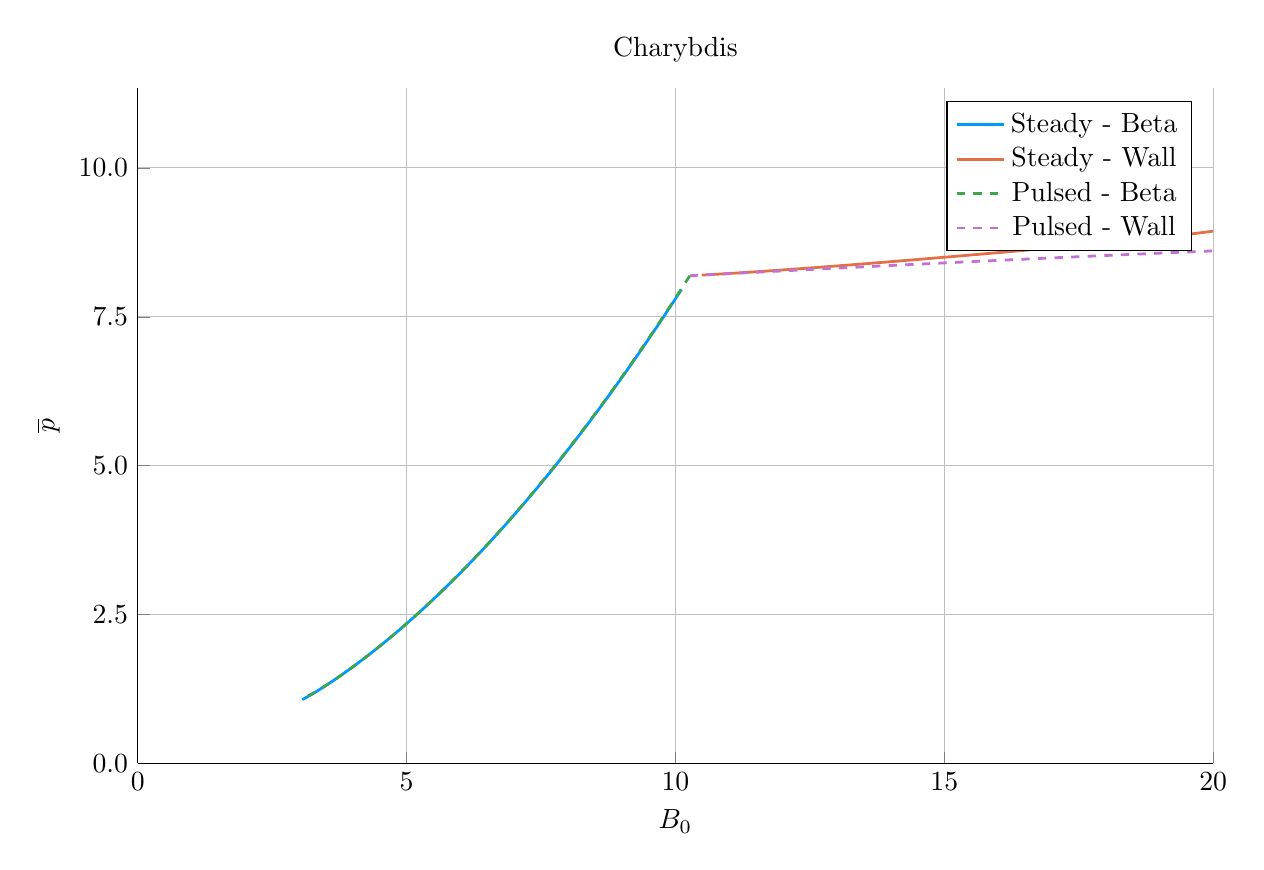
\begin{tikzpicture}[]
\begin{axis}[height = {101.6mm}, ylabel = {$\overline {p}$}, title = {Charybdis}, xmin = {0.0}, xmax = {20.0}, ymax = {11.344526307031618}, xlabel = {${B}_{0}$}, {unbounded coords=jump, scaled x ticks = false, xticklabel style={rotate = 0}, xmajorgrids = true, xtick = {0.0,5.0,10.0,15.0,20.0}, xticklabels = {0,5,10,15,20}, xtick align = inside, axis lines* = left, scaled y ticks = false, yticklabel style={rotate = 0}, ymajorgrids = true, ytick = {0.0,2.5,5.0,7.5,10.0}, yticklabels = {0.0,2.5,5.0,7.5,10.0}, ytick align = inside, axis lines* = left,     xshift = 0.0mm,
    yshift = 0.0mm,
    axis background/.style={fill={rgb,1:red,1.00000000;green,1.00000000;blue,1.00000000}}
, colorbar style={title=}}, ymin = {0.0}, width = {152.4mm}]\addplot+ [color = {rgb,1:red,0.00000000;green,0.60560316;blue,0.97868012},
draw opacity=1.0,
line width=1,
solid,mark = none,
mark size = 2.0,
mark options = {
    color = {rgb,1:red,0.00000000;green,0.00000000;blue,0.00000000}, draw opacity = 1.0,
    fill = {rgb,1:red,0.00000000;green,0.60560316;blue,0.97868012}, fill opacity = 1.0,
    line width = 1,
    rotate = 0,
    solid
}]coordinates {
(10.112818033153026, 7.9583125123879475)
(9.722156888543116, 7.421025940150145)
(9.357875603858393, 6.935991005854811)
(9.017653755630063, 6.496940579288293)
(8.6995124437054, 6.098597247083702)
(8.401566530516865, 5.73627060052837)
(8.122163706328223, 5.405946227791708)
(7.859819415455661, 5.104138041193254)
(7.613196557650265, 4.827808660713596)
(7.381088038653343, 4.574303257007293)
(7.162401716104116, 4.341294340666294)
(6.956147367527331, 4.12673549649745)
(6.761425371986388, 3.928822460925428)
(6.577416849463348, 3.7459602538630707)
(6.403375044688587, 3.5767353234089283)
(6.2386177769852695, 3.419891857544796)
(6.0825208065966905, 3.2743115733158015)
(5.934511989185341, 3.1389964165423176)
(5.794066116682695, 3.0130537124638765)
(5.660700347012839, 2.895683377055672)
(5.533970150598111, 2.786166876378168)
(5.413465705416883, 2.683857667486883)
(5.298808685607224, 2.5881729018421016)
(5.189649392059402, 2.4985862039383124)
(5.085664187259174, 2.414621373898747)
(4.986553195072601, 2.335846880583606)
(4.892038235455667, 2.2618710360871535)
(4.801860966679364, 2.1923377579539784)
(4.7157812114040425, 2.1269228397010105)
(4.633575445956479, 2.065330661993055)
(4.5550354347559185, 2.007291286689251)
(4.479966994069385, 1.9525578842853164)
(4.408188871204256, 1.9009044522862504)
(4.33953172691477, 1.8521237879761667)
(4.273837210246432, 1.8060256840838271)
(4.210957116299974, 1.7624353201214684)
(4.15075261849161, 1.7211918258218595)
(4.0930935678432965, 1.6821469962156288)
(4.037857852672517, 1.6451641405594921)
(3.9849308127842145, 1.6101170496168133)
(3.9342047029103653, 1.576889067761522)
(3.8855782007091695, 1.5453722580747524)
(3.838955955133626, 1.5154666500693676)
(3.7942481714200484, 1.4870795609464889)
(3.7513702293348077, 1.4601249823873848)
(3.710242331663442, 1.434523025840125)
(3.6707891802306123, 1.4101994200907546)
(3.6329396770109583, 1.3870850556333698)
(3.5966266481325166, 1.365115570986201)
(3.5617865887889004, 1.344230976653508)
(3.5283594272686503, 1.324375312918108)
(3.496288306480746, 1.3054963380738451)
(3.465519381509793, 1.2875452440818642)
(3.4360016318699595, 1.2704763969621373)
(3.4076866872513096, 1.254247099522471)
(3.380528665662031, 1.2388173742825344)
(3.3544840229690007, 1.2241497646762676)
(3.3295114129297314, 1.2102091528168961)
(3.3055715568879336, 1.1969625922851688)
(3.2826271223788512, 1.1843791545596674)
(3.260642607548369, 1.172429786292078)
(3.239584247604666, 1.1610871871965214)
(3.2194198921826622, 1.1503256748878254)
(3.2001189373344725, 1.140121090192475)
(3.181652227422265, 1.1304506876814424)
(3.163991977015565, 1.1212930433437895)
(3.1471116955378684, 1.1126279678446946)
(3.130986116696265, 1.104436426316808)
(3.115591132350856, 1.096700464135318)
(3.1009037305081053, 1.0894031381780074)
(3.0869019371473265, 1.0825284531174255)
(3.0735647616124355, 1.0760613023336338)
(3.0608721453218655, 1.0699874130729472)
};
\addlegendentry{Steady - Beta}
\addplot+ [color = {rgb,1:red,0.88887350;green,0.43564919;blue,0.27812294},
draw opacity=1.0,
line width=1,
solid,mark = none,
mark size = 2.0,
mark options = {
    color = {rgb,1:red,0.00000000;green,0.00000000;blue,0.00000000}, draw opacity = 1.0,
    fill = {rgb,1:red,0.88887350;green,0.43564919;blue,0.27812294}, fill opacity = 1.0,
    line width = 1,
    rotate = 0,
    solid
}]coordinates {
(20.758867641064707, 9.068389085509327)
(20.346250098246923, 8.97855440249835)
(19.57104597888471, 8.888106023504818)
(18.681781921115476, 8.802163774844665)
(17.775790175980152, 8.722297405668543)
(16.896654716492492, 8.648935187995837)
(16.063927450323227, 8.582039618462003)
(15.285557510665852, 8.52137442728336)
(14.563500533069154, 8.466617155991399)
(13.896568848875791, 8.417413070923242)
(13.281970890030232, 8.373402606013808)
(12.716170469467318, 8.334235643376688)
(12.195372283741088, 8.299578803865158)
(11.715794270833433, 8.269118865696244)
(11.273815669498969, 8.242563987838693)
(10.866051794088186, 8.219643682457138)
(10.489365023931143, 8.200107143500851)
};
\addlegendentry{Steady - Wall}
\addplot+ [color = {rgb,1:red,0.24222430;green,0.64327509;blue,0.30444865},
draw opacity=1.0,
line width=1,
dashed,mark = none,
mark size = 2.0,
mark options = {
    color = {rgb,1:red,0.00000000;green,0.00000000;blue,0.00000000}, draw opacity = 1.0,
    fill = {rgb,1:red,0.24222430;green,0.64327509;blue,0.30444865}, fill opacity = 1.0,
    line width = 1,
    rotate = 0,
    solid
}]coordinates {
(10.26788634689966, 8.189607873273022)
(9.953967652326213, 7.749796720734348)
(9.567926244368271, 7.224666023807497)
(9.207974394987358, 6.750682157979298)
(8.871841888699304, 6.321735242048715)
(8.557505525932248, 5.932576480084717)
(8.263156925406376, 5.578679182258823)
(7.9871752024348766, 5.256124950600166)
(7.728103682045175, 4.961509993893182)
(7.484629973620137, 4.691867642596592)
(7.255568856523303, 4.444603968241192)
(7.039847526735421, 4.217444057404293)
(6.836492834698909, 4.0083869902619025)
(6.644620209081183, 3.815667963435069)
(6.463424013335149, 3.637726302384703)
(6.2921691243175495, 3.4731783494540105)
(6.13018355681404, 3.320794404495876)
(5.97685198655569, 3.1794790473607746)
(5.831610044919842, 3.0482542904886434)
(5.693939286027163, 2.9262451155368945)
(5.563362729090489, 2.812667013471374)
(5.439440906144732, 2.7068152250667086)
(5.321768347746793, 2.608055422419593)
(5.209970453003084, 2.515815618819179)
(5.103700692769835, 2.4295791244455693)
(5.002638109938164, 2.3488784015950777)
(4.906485077678376, 2.2732896891904857)
(4.814965286571576, 2.2024282907336286)
(4.727821933804548, 2.1359444346131546)
(4.644816091323922, 2.0735196295675578)
(4.565725232806084, 2.0148634495286997)
(4.490341901840154, 1.9597106916581004)
(4.418472505906755, 1.9078188594571228)
(4.349936222622964, 1.8589659296429766)
(4.284564006352339, 1.8129483672432778)
(4.222197684694192, 1.7695793582518493)
(4.162689135592264, 1.7286872333449708)
(4.105899536872315, 1.690114059702365)
(4.051698680949713, 1.6537143810058763)
(3.9999643482627323, 1.6193540882830624)
(3.9505817337017928, 1.5869094064904927)
(3.903442920928527, 1.5562659836456025)
(3.858446400032002, 1.5273180709693464)
(3.8154966244515616, 1.499967783926687)
(3.7745036035252744, 1.47412443528753)
(3.7353825273991994, 1.4497039324003564)
(3.6980534213689746, 1.426628231801804)
(3.6624408270205375, 1.4048248450941176)
(3.62847350780097, 1.3842263907285874)
(3.5960841768845415, 1.3647701869494269)
(3.565209245407392, 1.3463978816914282)
(3.5357885893311605, 1.3290551156980193)
(3.5077653333614305, 1.312691215540287)
(3.4810856504959875, 1.297258913582693)
(3.4556985759109375, 1.2827140922618574)
(3.4315558340122845, 1.2690155503279663)
(3.408611677587535, 1.2561247889480192)
(3.3868227380888998, 1.2440058157914007)
(3.36614788616562, 1.2326249654134387)
(3.3465481016421226, 1.2219507344266094)
(3.327986352208224, 1.211953630102413)
(3.3104274769652595, 1.20260602913631)
(3.2938380965241474, 1.1938820598138524)
(3.278186482171801, 1.185757463580358)
(3.263442495132517, 1.178209506801885)
(3.2495774839156075, 1.1712168702313421)
(3.236564206241785, 1.164759558459252)
(3.224376752844934, 1.1588188143537892)
(3.212990475972638, 1.1533770399408283)
(3.2023819222517877, 1.148417723182766)
(3.192528769611062, 1.1439253701643137)
(3.1834097679780142, 1.1398854422392488)
(3.1750046834890777, 1.1362842977318812)
(3.1672942459724482, 1.1331091378241047)
};
\addlegendentry{Pulsed - Beta}
\addplot+ [color = {rgb,1:red,0.76444018;green,0.44411178;blue,0.82429754},
draw opacity=1.0,
line width=1,
dashed,mark = none,
mark size = 2.0,
mark options = {
    color = {rgb,1:red,0.00000000;green,0.00000000;blue,0.00000000}, draw opacity = 1.0,
    fill = {rgb,1:red,0.76444018;green,0.44411178;blue,0.82429754}, fill opacity = 1.0,
    line width = 1,
    rotate = 0,
    solid
}]coordinates {
(48.990476413653056, 9.453771922526348)
(42.83950920694117, 9.306252585805208)
(37.687790427214495, 9.172172663451207)
(33.33937742845888, 9.05012027487084)
(29.64296398154308, 8.938871992925128)
(26.48039367255613, 8.83736301771481)
(23.758442882319894, 8.744662760028714)
(21.402860298405816, 8.659954735896104)
(19.353987387634486, 8.582519919278019)
(17.563502020363714, 8.511722885598683)
(15.991970371213752, 8.44700022140578)
(14.606987499719377, 8.387850783306833)
(13.381751501116137, 8.33382747486016)
(12.293960329570087, 8.284530275188235)
(11.32495111804522, 8.239600304840708)
(10.459023415380802, 8.198714755061442)
(10.26788634689966, 8.189607873273022)
};
\addlegendentry{Pulsed - Wall}
\end{axis}

\end{tikzpicture}

    \end{adjustbox}
        \caption{Charybdis}
    \end{subfigure}
    \hfill
    \begin{subfigure}[t]{0.45\textwidth}
        \centering
    \begin{adjustbox}{width=\textwidth}
      \Large
      \begin{tikzpicture}[]
\begin{axis}[height = {101.6mm}, ylabel = {$\overline {p}$}, title = {Proteus}, xmin = {0.0}, xmax = {20.0}, ymax = {8.221153650881353}, xlabel = {${B}_{0}$}, {unbounded coords=jump, scaled x ticks = false, xticklabel style={rotate = 0}, xmajorgrids = true, xtick = {0.0,5.0,10.0,15.0,20.0}, xticklabels = {0,5,10,15,20}, xtick align = inside, axis lines* = left, scaled y ticks = false, yticklabel style={rotate = 0}, ymajorgrids = true, ytick = {0.0,2.0,4.0,6.0,8.0}, yticklabels = {0,2,4,6,8}, ytick align = inside, axis lines* = left,     xshift = 0.0mm,
    yshift = 0.0mm,
    axis background/.style={fill={rgb,1:red,1.00000000;green,1.00000000;blue,1.00000000}}
, colorbar style={title=}}, ymin = {0.0}, width = {152.4mm}]\addplot+ [color = {rgb,1:red,0.00000000;green,0.60560316;blue,0.97868012},
draw opacity=1.0,
line width=1,
solid,mark = none,
mark size = 2.0,
mark options = {
    color = {rgb,1:red,0.00000000;green,0.00000000;blue,0.00000000}, draw opacity = 1.0,
    fill = {rgb,1:red,0.00000000;green,0.60560316;blue,0.97868012}, fill opacity = 1.0,
    line width = 1,
    rotate = 0,
    solid
}]coordinates {
(4.658732060637907, 0.5178850991814221)
(4.211109766361548, 0.5901090170938682)
(3.9293920326356777, 0.6706294868376301)
(3.7651903683456465, 0.7607821823857104)
(3.6776039543745567, 0.8606801122549695)
(3.6402437753208394, 0.9701410974242217)
(3.6366994671255806, 1.0889506687305381)
(3.656621534643579, 1.2169227139444314)
(3.693300156736026, 1.3539039774890367)
(3.7422515017241134, 1.4997653650140765)
(3.865532743079537, 1.8176754932537085)
(3.936096932264377, 1.9895070708630855)
(4.010907188015084, 2.1697740073895155)
(4.089072356933184, 2.358356185011204)
(4.169903401491354, 2.5551241072307835)
(4.252857906625248, 2.7599375621672912)
(4.337501757261618, 2.972644834346649)
(4.42348218754058, 3.193082337621686)
(4.5983381267510195, 3.656434381707281)
(4.686766232902671, 3.8989633349682533)
(4.775618142770625, 4.148452404136471)
(4.864743502376605, 4.404682698149458)
(4.927312314219091, 4.588196259305366)
};
\addlegendentry{Pulsed - Kink}
\addplot+ [color = {rgb,1:red,0.88887350;green,0.43564919;blue,0.27812294},
draw opacity=1.0,
line width=1,
solid,mark = none,
mark size = 2.0,
mark options = {
    color = {rgb,1:red,0.00000000;green,0.00000000;blue,0.00000000}, draw opacity = 1.0,
    fill = {rgb,1:red,0.88887350;green,0.43564919;blue,0.27812294}, fill opacity = 1.0,
    line width = 1,
    rotate = 0,
    solid
}]coordinates {
(4.927312314219091, 4.588196259305366)
(4.984545814413324, 4.661509991488243)
(5.17452482724068, 4.908243268425499)
(5.362091669637646, 5.156912736454039)
(5.54700293215903, 5.406966492547543)
(5.729042482638278, 5.657877514372715)
(5.908022832274664, 5.909149637868065)
(6.083785777786694, 6.160322381748082)
(6.256202341425288, 6.410974518609055)
(6.324169421042356, 6.510945391637745)
};
\addlegendentry{Pulsed - Beta}
\addplot+ [color = {rgb,1:red,0.24222430;green,0.64327509;blue,0.30444865},
draw opacity=1.0,
line width=1,
solid,mark = none,
mark size = 2.0,
mark options = {
    color = {rgb,1:red,0.00000000;green,0.00000000;blue,0.00000000}, draw opacity = 1.0,
    fill = {rgb,1:red,0.24222430;green,0.64327509;blue,0.30444865}, fill opacity = 1.0,
    line width = 1,
    rotate = 0,
    solid
}]coordinates {
(6.324169421042356, 6.510945391637745)
(6.727338549778396, 6.526506139925002)
(7.320469048424473, 6.547612990538456)
(7.835746509376305, 6.565018654158398)
(8.290245520072391, 6.580373530609689)
(8.696162676727877, 6.594675052963156)
(9.0624397222742, 6.608548283632356)
(9.395798186463841, 6.62239478853408)
(9.701405747258567, 6.636476310012618)
(10.244760202900984, 6.665969558295109)
(10.930275827723788, 6.714664499426381)
(11.131878682735255, 6.732204582219528)
(11.50278450645086, 6.7692640538633295)
(11.83715172742864, 6.808892337209671)
(11.992609772603878, 6.829630927312101)
(12.141110720831467, 6.850961375734461)
};
\addlegendentry{Pulsed - Wall}
\end{axis}

\end{tikzpicture}

    \end{adjustbox}
        \caption{Proteus}
    \end{subfigure}
    \hfill \hfill ~\\ ~\\ ~\\ ~\\
    \hfill
    \begin{subfigure}[t]{0.45\textwidth}
        \centering
    \begin{adjustbox}{width=\textwidth}
      \Large
      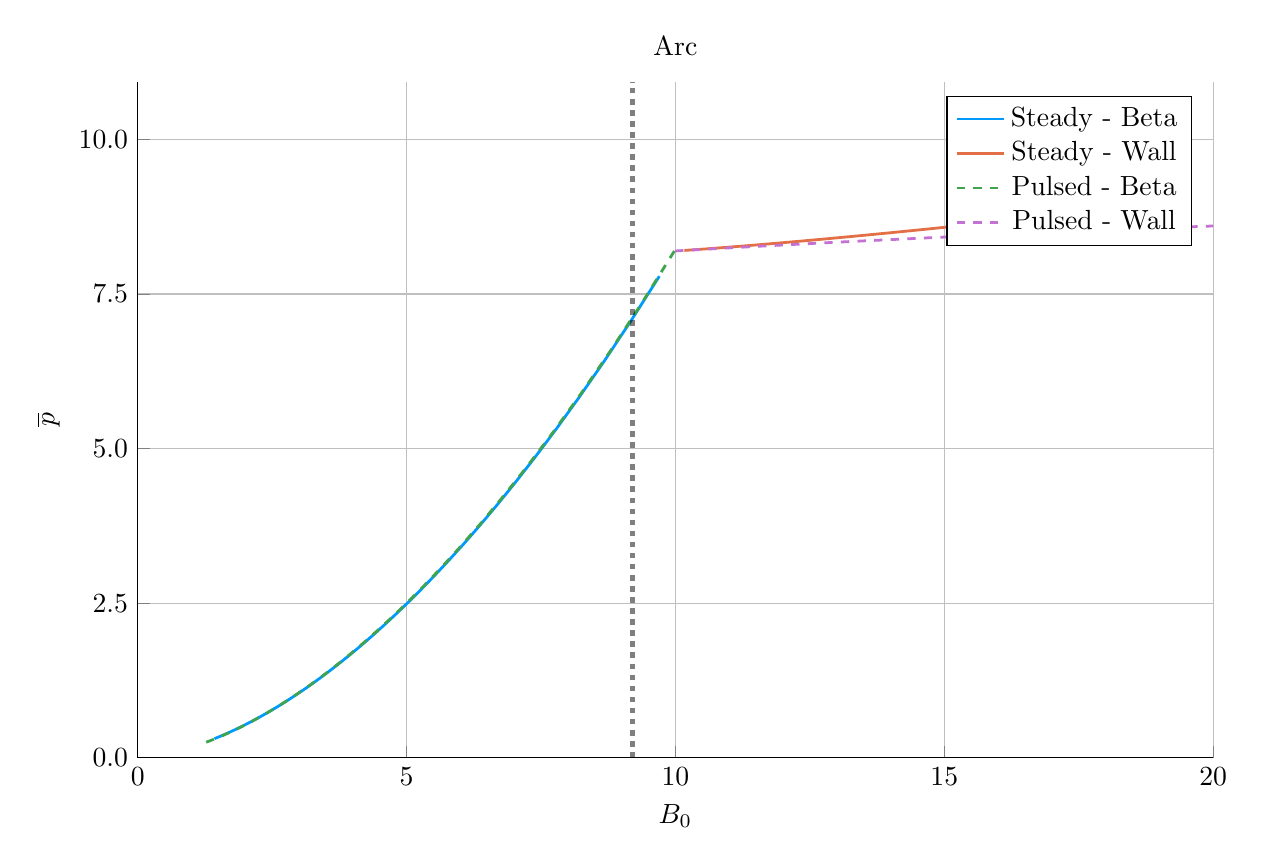
\begin{tikzpicture}[]
\begin{axis}[height = {101.6mm}, ylabel = {$\overline {p}$}, title = {Arc}, xmin = {0.0}, xmax = {20.0}, ymax = {10.926180969301674}, xlabel = {${B}_{0}$}, {unbounded coords=jump, scaled x ticks = false, xticklabel style={rotate = 0}, xmajorgrids = true, xtick = {0.0,5.0,10.0,15.0,20.0}, xticklabels = {0,5,10,15,20}, xtick align = inside, axis lines* = left, scaled y ticks = false, yticklabel style={rotate = 0}, ymajorgrids = true, ytick = {0.0,2.5,5.0,7.5,10.0}, yticklabels = {0.0,2.5,5.0,7.5,10.0}, ytick align = inside, axis lines* = left,     xshift = 0.0mm,
    yshift = 0.0mm,
    axis background/.style={fill={rgb,1:red,1.00000000;green,1.00000000;blue,1.00000000}}
, colorbar style={title=}}, ymin = {0.0}, width = {152.4mm}]\addplot+ [color = {rgb,1:red,0.00000000;green,0.60560316;blue,0.97868012},
draw opacity=1.0,
line width=1,
solid,mark = none,
mark size = 2.0,
mark options = {
    color = {rgb,1:red,0.00000000;green,0.00000000;blue,0.00000000}, draw opacity = 1.0,
    fill = {rgb,1:red,0.00000000;green,0.60560316;blue,0.97868012}, fill opacity = 1.0,
    line width = 1,
    rotate = 0,
    solid
}]coordinates {
(9.701206080853105, 7.787955755021093)
(9.162315904693079, 7.051651042713914)
(8.664301107137337, 6.400059822567223)
(8.203576462497304, 5.822163941026312)
(7.776718537485166, 5.308305932197296)
(7.380720231870917, 4.85030660077028)
(7.012886014999712, 4.441159545362493)
(6.670795005901889, 4.074845420367799)
(6.352268997292712, 3.746178328906164)
(6.055344682097163, 3.450678325669481)
(5.778249464564785, 3.1844652225883903)
(5.519380338856715, 2.9441698424426552)
(5.2772854007125325, 2.726859615959229)
(5.050647625972996, 2.5299760120957133)
(4.838270606140816, 2.35128176372989)
(4.639065978019038, 2.1888162283724957)
(4.4520423235376105, 2.040857526170124)
(4.276295348572609, 1.9058903411238468)
(4.110999177018484, 1.7825784683554267)
(3.9553986195015125, 1.6697413499493832)
(3.8088022956698633, 1.5663339718702352)
(3.6705765055641186, 1.4714296005854386)
(3.54013975965751, 1.3842049249687662)
(3.4169578891619192, 1.3039272405056976)
(3.30053966845824, 1.2299433717107324)
(3.1904328903033052, 1.1616700773436754)
(3.086220842019516, 1.098585723362249)
(2.9875191373772063, 1.0402230420856027)
(2.8939728644914635, 0.9861628239914726)
(2.8052540149097247, 0.9360284119196484)
(2.7210591632720242, 0.8894808870098675)
(2.6411073705789065, 0.8462148521196278)
(2.565138287279709, 0.8059547322817329)
(2.492910435164382, 0.768451523411881)
(2.4241996494611984, 0.7334799303234187)
(2.3587976646588236, 0.7008358434465796)
(2.296510829425685, 0.6703341107280705)
(2.237158937627476, 0.6418065672072185)
(2.180574163874242, 0.6151002898943585)
(2.126600093288366, 0.5900760499569412)
(2.075090836295778, 0.5666069379647121)
(2.0259102202234582, 0.5445771411552895)
(1.978931050353818, 0.5238808544368901)
(1.9340344338545452, 0.504421309214282)
(1.8911091606836798, 0.48610990616509375)
(1.8500511361739687, 0.4688654398542168)
(1.8107628605384507, 0.4526134045959324)
(1.773152951016952, 0.437285372290203)
(1.7371357028100902, 0.42281843410159214)
(1.7026306853269466, 0.40915469884020483)
(1.6695623706125668, 0.3962408417661064)
(1.6378597911249178, 0.3840276982890354)
(1.607456224302725, 0.372469897689607)
(1.5782889016090462, 0.3615255325596127)
(1.5502987399539199, 0.35115586015858613)
(1.5234300935954943, 0.3413250323213126)
(1.4976305247952577, 0.3319998509344066)
(1.4728505916614916, 0.3231495463367305)
(1.4490436517578602, 0.31474557629434374)
(1.4261656801829077, 0.3067614434611321)
};
\addlegendentry{Steady - Beta}
\addplot+ [color = {rgb,1:red,0.88887350;green,0.43564919;blue,0.27812294},
draw opacity=1.0,
line width=1,
solid,mark = none,
mark size = 2.0,
mark options = {
    color = {rgb,1:red,0.00000000;green,0.00000000;blue,0.00000000}, draw opacity = 1.0,
    fill = {rgb,1:red,0.88887350;green,0.43564919;blue,0.27812294}, fill opacity = 1.0,
    line width = 1,
    rotate = 0,
    solid
}]coordinates {
(19.394007482712425, 9.105150807751395)
(18.932196567189358, 9.01069147020663)
(18.296989378345195, 8.920028762512676)
(17.587029315408756, 8.834810462148925)
(16.847882407994106, 8.755400742376121)
(16.111374502564406, 8.681959138040654)
(15.396027314547156, 8.614412652055668)
(14.710952688793137, 8.552522407908596)
(14.06168447794857, 8.496032613589257)
(13.450465418483889, 8.444654873548563)
(12.877644538645335, 8.39809478260268)
(12.342394470642008, 8.356062046626297)
(11.843182246608265, 8.318276332900204)
(11.376441269625893, 8.28440059784499)
(10.944966372727551, 8.254392355607594)
(10.541663878705513, 8.227805045250905)
(10.165908182236457, 8.204482050940095)
};
\addlegendentry{Steady - Wall}
\addplot+ [color = {rgb,1:red,0.24222430;green,0.64327509;blue,0.30444865},
draw opacity=1.0,
line width=1,
dashed,mark = none,
mark size = 2.0,
mark options = {
    color = {rgb,1:red,0.00000000;green,0.00000000;blue,0.00000000}, draw opacity = 1.0,
    fill = {rgb,1:red,0.24222430;green,0.64327509;blue,0.30444865}, fill opacity = 1.0,
    line width = 1,
    rotate = 0,
    solid
}]coordinates {
(9.980483622051658, 8.195219263193664)
(9.392786903460065, 7.377227717670988)
(8.79273598103983, 6.5811843482923535)
(8.23820290909994, 5.881064228944964)
(7.725182218401588, 5.264095572566794)
(7.250078106370205, 4.719377620875317)
(6.80965553466646, 4.23757979878168)
(6.400998063035608, 3.8106937592785157)
(6.0214713600430425, 3.431828200771469)
(5.668691517461799, 3.095038432241675)
(5.340497445229901, 2.7951842896444266)
(5.034926745580058, 2.5278112800143946)
(4.750194564008521, 2.2890508304972803)
(4.484674995755211, 2.0755363101823026)
(4.236884692979903, 1.8843321202884853)
(4.00546837264544, 1.712873648854056)
(3.7891859704718387, 1.5589162870833615)
(3.5869012239550364, 1.4204920270856354)
(3.3975714987448393, 1.295872421279243)
(3.2202386987489797, 1.1835368949703546)
(3.0540211220494466, 1.0821455755001503)
(2.8981061427709687, 0.9905159416987992)
(2.7517436139566023, 0.9076027123374337)
(2.6142398986781377, 0.8324804866958566)
(2.4849524463010138, 0.7643287281154789)
(2.363284838174807, 0.7024187455448467)
(2.248682232019848, 0.646102381031827)
(2.140627136740878, 0.5948021547833593)
(2.038635448877246, 0.5480026552795989)
(1.9422526775794744, 0.5052429910940035)
(1.8510502754751532, 0.46611014427001946)
(1.7646219756564088, 0.4302330826713539)
(1.6825800061969869, 0.3972775004758068)
(1.6045510059627948, 0.3669410609704078)
(1.53017138625397, 0.3389490117745717)
(1.4590817483192686, 0.3130500249001194)
(1.3909197311384796, 0.28901207317609945)
(1.3253102336217724, 0.26661807080873934)
(1.261851128383913, 0.24566083615905465)
(1.20009089049112, 0.22593657860936153)
(1.1394908096975784, 0.20723531230777545)
};
\addlegendentry{Pulsed - Beta}
\addplot+ [color = {rgb,1:red,0.76444018;green,0.44411178;blue,0.82429754},
draw opacity=1.0,
line width=1,
dashed,mark = none,
mark size = 2.0,
mark options = {
    color = {rgb,1:red,0.00000000;green,0.00000000;blue,0.00000000}, draw opacity = 1.0,
    fill = {rgb,1:red,0.76444018;green,0.44411178;blue,0.82429754}, fill opacity = 1.0,
    line width = 1,
    rotate = 0,
    solid
}]coordinates {
(29.27715761652869, 8.869302576453649)
(25.4410619834368, 8.766170137139135)
(22.158819835998365, 8.669604452730885)
(19.342453256965573, 8.579059039729174)
(16.919364280634177, 8.494045731653955)
(14.829378672669455, 8.414127307177784)
(13.022412368922526, 8.338911194240602)
(11.456617692058645, 8.268044073337753)
(10.096901921254785, 8.201207235220023)
(9.980483622051658, 8.195219263193664)
};
\addlegendentry{Pulsed - Wall}
\addplot+ [color = {rgb,1:red,0.00000000;green,0.00000000;blue,0.00000000},
draw opacity=0.5,
line width=2,
dotted,mark = none,
mark size = 2.0,
mark options = {
    color = {rgb,1:red,0.00000000;green,0.00000000;blue,0.00000000}, draw opacity = 0.5,
    fill = {rgb,1:red,0.00000000;green,0.00000000;blue,0.00000000}, fill opacity = 0.5,
    line width = 1,
    rotate = 0,
    solid
},forget plot]coordinates {
(0.0, NaN)
(20.0, NaN)
};
\addplot+ [color = {rgb,1:red,0.00000000;green,0.00000000;blue,0.00000000},
draw opacity=0.5,
line width=2,
dotted,mark = none,
mark size = 2.0,
mark options = {
    color = {rgb,1:red,0.00000000;green,0.00000000;blue,0.00000000}, draw opacity = 0.5,
    fill = {rgb,1:red,0.00000000;green,0.00000000;blue,0.00000000}, fill opacity = 0.5,
    line width = 1,
    rotate = 0,
    solid
},forget plot]coordinates {
(9.2, 0.0)
(9.2, 10.926180969301674)
};
\addplot+[draw=none, color = {rgb,1:red,0.00000000;green,0.00000000;blue,0.00000000},
draw opacity=0.5,
line width=0,
solid,mark = *,
mark size = 2.0,
mark options = {
    color = {rgb,1:red,0.00000000;green,0.00000000;blue,0.00000000}, draw opacity = 0.5,
    fill = {rgb,1:red,0.00000000;green,0.00000000;blue,0.00000000}, fill opacity = 0.5,
    line width = 1,
    rotate = 0,
    solid
},forget plot] coordinates {
(9.2, NaN)
};
\end{axis}

\end{tikzpicture}

    \end{adjustbox}
        \caption{ARC}
    \end{subfigure}
    \hfill
    \begin{subfigure}[t]{0.45\textwidth}
        \centering
    \begin{adjustbox}{width=\textwidth}
      \Large
      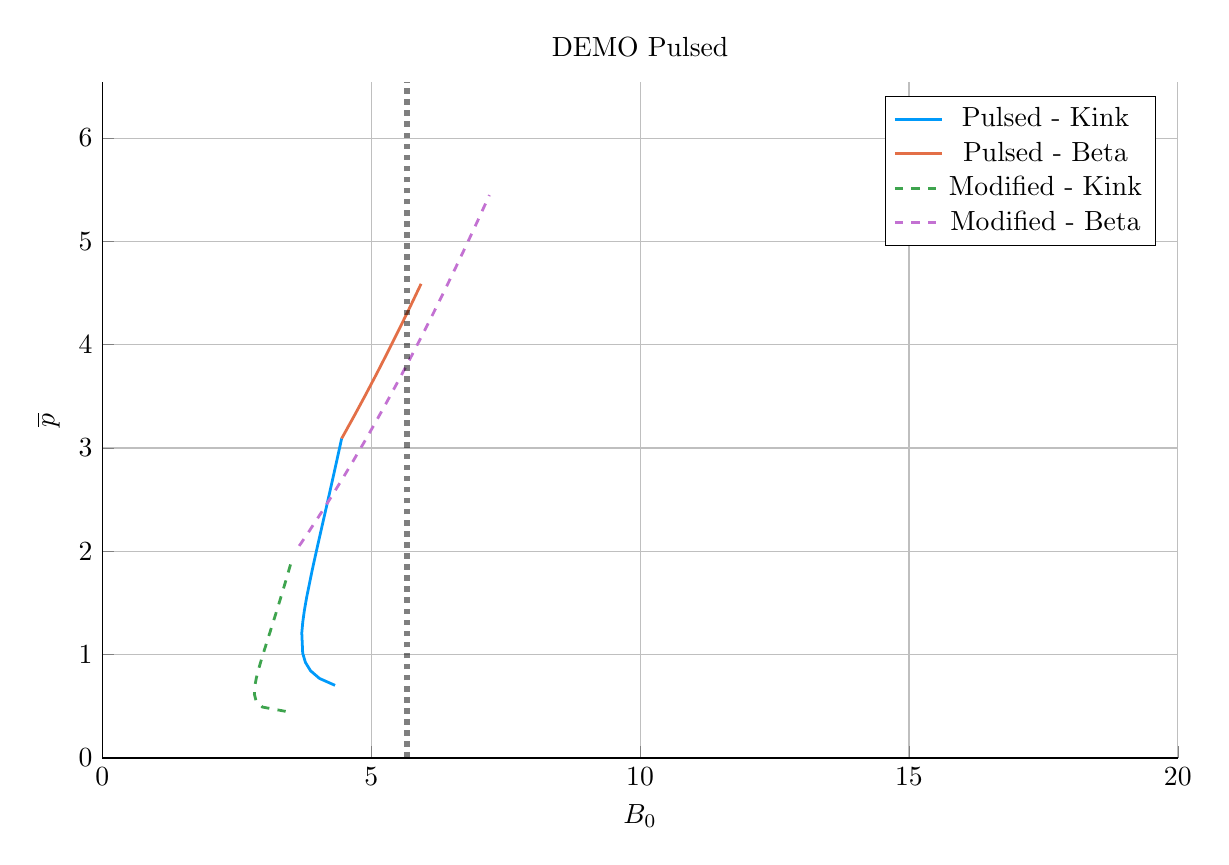
\begin{tikzpicture}[]
\begin{axis}[height = {101.6mm}, ylabel = {$\overline {p}$}, title = {DEMO Pulsed}, xmin = {0.0}, xmax = {20.0}, ymax = {6.537850901250805}, xlabel = {${B}_{0}$}, {unbounded coords=jump, scaled x ticks = false, xticklabel style={rotate = 0}, xmajorgrids = true, xtick = {0.0,5.0,10.0,15.0,20.0}, xticklabels = {0,5,10,15,20}, xtick align = inside, axis lines* = left, scaled y ticks = false, yticklabel style={rotate = 0}, ymajorgrids = true, ytick = {0.0,1.0,2.0,3.0,4.0,5.0,6.0}, yticklabels = {0,1,2,3,4,5,6}, ytick align = inside, axis lines* = left,     xshift = 0.0mm,
    yshift = 0.0mm,
    axis background/.style={fill={rgb,1:red,1.00000000;green,1.00000000;blue,1.00000000}}
, colorbar style={title=}}, ymin = {0.0}, width = {152.4mm}]\addplot+ [color = {rgb,1:red,0.00000000;green,0.60560316;blue,0.97868012},
draw opacity=1.0,
line width=1,
solid,mark = none,
mark size = 2.0,
mark options = {
    color = {rgb,1:red,0.00000000;green,0.00000000;blue,0.00000000}, draw opacity = 1.0,
    fill = {rgb,1:red,0.00000000;green,0.60560316;blue,0.97868012}, fill opacity = 1.0,
    line width = 1,
    rotate = 0,
    solid
}]coordinates {
(4.327031075670194, 0.7028031640947805)
(4.038214026054326, 0.7698036844931152)
(3.8713719163129245, 0.8443448144092149)
(3.7758613845615545, 0.9259542560730941)
(3.7257856761317214, 1.014326207681088)
(3.7090473695925437, 1.2107278386279736)
(3.727711597554826, 1.3186260367708318)
(3.7586131667481433, 1.4329756622073844)
(3.799052518631718, 1.553800358442639)
(3.901290136389271, 1.8150455990056997)
(3.960577465316514, 1.9555744496412666)
(4.0241209645210345, 2.1027883266322367)
(4.0912717805663785, 2.2567509739739426)
(4.161514602943343, 2.4175266863222564)
(4.2344343960723005, 2.585179148763694)
(4.309692554546368, 2.7597705284707077)
(4.450417240491067, 3.0922614007783964)
};
\addlegendentry{Pulsed - Kink}
\addplot+ [color = {rgb,1:red,0.88887350;green,0.43564919;blue,0.27812294},
draw opacity=1.0,
line width=1,
solid,mark = none,
mark size = 2.0,
mark options = {
    color = {rgb,1:red,0.00000000;green,0.00000000;blue,0.00000000}, draw opacity = 1.0,
    fill = {rgb,1:red,0.88887350;green,0.43564919;blue,0.27812294}, fill opacity = 1.0,
    line width = 1,
    rotate = 0,
    solid
}]coordinates {
(4.450417240491067, 3.0922614007783964)
(4.490148631384312, 3.129020144234441)
(4.692490181445514, 3.319283176152804)
(4.8960344619053355, 3.5158038843820316)
(5.100651132702229, 3.718497413182538)
(5.306202822090688, 3.927262261143742)
(5.512545696627038, 4.141979779065389)
(5.719530043226767, 4.362513842680247)
(5.927000883375481, 4.588710713693877)
};
\addlegendentry{Pulsed - Beta}
\addplot+ [color = {rgb,1:red,0.24222430;green,0.64327509;blue,0.30444865},
draw opacity=1.0,
line width=1,
dashed,mark = none,
mark size = 2.0,
mark options = {
    color = {rgb,1:red,0.00000000;green,0.00000000;blue,0.00000000}, draw opacity = 1.0,
    fill = {rgb,1:red,0.24222430;green,0.64327509;blue,0.30444865}, fill opacity = 1.0,
    line width = 1,
    rotate = 0,
    solid
}]coordinates {
(3.4087424183072135, 0.45099910075611205)
(2.977074181068944, 0.4927398533402812)
(2.8592500074202523, 0.550921624204788)
(2.827199220063259, 0.6176021690387108)
(2.8339789008667826, 0.6910982334726382)
(2.862412302880871, 0.7708502835005886)
(2.9044598258085443, 0.8566555291245366)
(2.95577893007882, 0.9484576740541925)
(3.0137895352525907, 1.046270321894979)
(3.076849710218805, 1.1501437144528015)
(3.1438583711612704, 1.2601484027082435)
(3.214045733980633, 1.3763664546005359)
(3.2868548955983727, 1.4988863592342698)
(3.361871149981842, 1.627799886106626)
(3.4387778750377818, 1.76320004278458)
(3.5173279629378453, 1.9051796810503774)
};
\addlegendentry{Modified - Kink}
\addplot+ [color = {rgb,1:red,0.76444018;green,0.44411178;blue,0.82429754},
draw opacity=1.0,
line width=1,
dashed,mark = none,
mark size = 2.0,
mark options = {
    color = {rgb,1:red,0.00000000;green,0.00000000;blue,0.00000000}, draw opacity = 1.0,
    fill = {rgb,1:red,0.76444018;green,0.44411178;blue,0.82429754}, fill opacity = 1.0,
    line width = 1,
    rotate = 0,
    solid
}]coordinates {
(3.6607028750648505, 2.0521650502532194)
(3.8574448036470477, 2.2041901592081676)
(4.056375867871351, 2.362513447000359)
(4.257366397480293, 2.5271287396356366)
(4.460279103534801, 2.6980149065835244)
(4.664969389370631, 2.875134762759023)
(4.871285596007394, 3.0584340806231745)
(5.07906923307514, 3.2478407223505603)
(5.288155233306219, 3.443263907724574)
(5.498372259673351, 3.6445936373209773)
(5.709543087166185, 3.8517002928382684)
(5.921485076209294, 4.064434437320309)
(6.134010749367255, 4.282626837356303)
(6.346928478632384, 4.5060887272499945)
(6.560043285872518, 4.734612331532486)
(6.773157754368795, 4.967971657138228)
(6.986073044284746, 5.205923560115345)
(7.198590001107076, 5.448209084375671)
};
\addlegendentry{Modified - Beta}
\addplot+ [color = {rgb,1:red,0.00000000;green,0.00000000;blue,0.00000000},
draw opacity=0.5,
line width=2,
dotted,mark = none,
mark size = 2.0,
mark options = {
    color = {rgb,1:red,0.00000000;green,0.00000000;blue,0.00000000}, draw opacity = 0.5,
    fill = {rgb,1:red,0.00000000;green,0.00000000;blue,0.00000000}, fill opacity = 0.5,
    line width = 1,
    rotate = 0,
    solid
},forget plot]coordinates {
(0.0, NaN)
(20.0, NaN)
};
\addplot+ [color = {rgb,1:red,0.00000000;green,0.00000000;blue,0.00000000},
draw opacity=0.5,
line width=2,
dotted,mark = none,
mark size = 2.0,
mark options = {
    color = {rgb,1:red,0.00000000;green,0.00000000;blue,0.00000000}, draw opacity = 0.5,
    fill = {rgb,1:red,0.00000000;green,0.00000000;blue,0.00000000}, fill opacity = 0.5,
    line width = 1,
    rotate = 0,
    solid
},forget plot]coordinates {
(5.667, 0.0)
(5.667, 6.537850901250805)
};
\addplot+[draw=none, color = {rgb,1:red,0.00000000;green,0.00000000;blue,0.00000000},
draw opacity=0.5,
line width=0,
solid,mark = *,
mark size = 2.0,
mark options = {
    color = {rgb,1:red,0.00000000;green,0.00000000;blue,0.00000000}, draw opacity = 0.5,
    fill = {rgb,1:red,0.00000000;green,0.00000000;blue,0.00000000}, fill opacity = 0.5,
    line width = 1,
    rotate = 0,
    solid
},forget plot] coordinates {
(5.667, NaN)
};
\end{axis}

\end{tikzpicture}

    \end{adjustbox}
        \caption{DEMO Pulsed}
    \end{subfigure}
    \hfill \hfill ~\\ ~\\ ~\\ ~\\
    \hfill
    \begin{subfigure}[t]{0.45\textwidth}
        \centering
    \begin{adjustbox}{width=\textwidth}
      \Large
      \begin{tikzpicture}[]
\begin{axis}[height = {101.6mm}, ylabel = {$\overline {p}$}, title = {Act I}, xmin = {0.0}, xmax = {20.0}, ymax = {10.158285290891627}, xlabel = {${B}_{0}$}, {unbounded coords=jump, scaled x ticks = false, xticklabel style={rotate = 0}, xmajorgrids = true, xtick = {0.0,5.0,10.0,15.0,20.0}, xticklabels = {0,5,10,15,20}, xtick align = inside, axis lines* = left, scaled y ticks = false, yticklabel style={rotate = 0}, ymajorgrids = true, ytick = {0.0,2.5,5.0,7.5,10.0}, yticklabels = {0.0,2.5,5.0,7.5,10.0}, ytick align = inside, axis lines* = left,     xshift = 0.0mm,
    yshift = 0.0mm,
    axis background/.style={fill={rgb,1:red,1.00000000;green,1.00000000;blue,1.00000000}}
, colorbar style={title=}}, ymin = {0.0}, width = {152.4mm}]\addplot+ [color = {rgb,1:red,0.00000000;green,0.60560316;blue,0.97868012},
draw opacity=1.0,
line width=1,
solid,mark = none,
mark size = 2.0,
mark options = {
    color = {rgb,1:red,0.00000000;green,0.00000000;blue,0.00000000}, draw opacity = 1.0,
    fill = {rgb,1:red,0.00000000;green,0.60560316;blue,0.97868012}, fill opacity = 1.0,
    line width = 1,
    rotate = 0,
    solid
}]coordinates {
(6.30336807958207, 7.693131492396803)
(6.162193069273141, 7.37246010607685)
(6.030717178404645, 7.080346094310556)
(5.908065509576601, 6.8135301596601625)
(5.793464904530972, 6.5692113671770205)
(5.686229631357383, 6.344971653765388)
(5.585749511271037, 6.138714646547947)
};
\addlegendentry{Steady - Beta}
\addplot+ [color = {rgb,1:red,0.88887350;green,0.43564919;blue,0.27812294},
draw opacity=1.0,
line width=1,
solid,mark = none,
mark size = 2.0,
mark options = {
    color = {rgb,1:red,0.00000000;green,0.00000000;blue,0.00000000}, draw opacity = 1.0,
    fill = {rgb,1:red,0.88887350;green,0.43564919;blue,0.27812294}, fill opacity = 1.0,
    line width = 1,
    rotate = 0,
    solid
}]coordinates {
(12.549536249695134, 8.46523774240969)
(11.658754653696462, 8.392195022608814)
(10.883719833507003, 8.326717838123047)
(10.206258129789394, 8.268176927821916)
(9.611335769312953, 8.215994712910126)
(9.086446934250878, 8.169640475751706)
(8.62129895070743, 8.12863515278107)
(8.207216040989662, 8.092536970226544)
(7.837119555085499, 8.060954238763868)
(7.505047858717157, 8.033529985493542)
(7.20604322925957, 8.009944154326424)
(6.935884710193303, 7.989904321533297)
(6.691016583192173, 7.973146692107348)
(6.468415485086983, 7.959431994617008)
};
\addlegendentry{Steady - Wall}
\addplot+ [color = {rgb,1:red,0.24222430;green,0.64327509;blue,0.30444865},
draw opacity=1.0,
line width=1,
dashed,mark = none,
mark size = 2.0,
mark options = {
    color = {rgb,1:red,0.00000000;green,0.00000000;blue,0.00000000}, draw opacity = 1.0,
    fill = {rgb,1:red,0.24222430;green,0.64327509;blue,0.30444865}, fill opacity = 1.0,
    line width = 1,
    rotate = 0,
    solid
}]coordinates {
(6.408263337806559, 7.954620448090888)
(6.408263337806564, 7.954620448090904)
(6.385466513301022, 7.900876758204875)
(6.245492502072912, 7.57505159227564)
(6.116010320461132, 7.280041556299232)
(5.9960421481916395, 7.012211959576142)
(5.884727159112828, 6.768456047828764)
(5.781304768121868, 6.546105698035388)
(5.685100648450046, 6.342859211417754)
(5.595515000321003, 6.156722568397863)
};
\addlegendentry{Pulsed - Beta}
\addplot+ [color = {rgb,1:red,0.76444018;green,0.44411178;blue,0.82429754},
draw opacity=1.0,
line width=1,
dashed,mark = none,
mark size = 2.0,
mark options = {
    color = {rgb,1:red,0.00000000;green,0.00000000;blue,0.00000000}, draw opacity = 1.0,
    fill = {rgb,1:red,0.76444018;green,0.44411178;blue,0.82429754}, fill opacity = 1.0,
    line width = 1,
    rotate = 0,
    solid
}]coordinates {
(12.684248532650473, 8.40187240241852)
(11.66307871570063, 8.333170036080388)
(10.781888309639141, 8.271584589435095)
(10.016282491385791, 8.216472046761803)
(9.346943280276514, 8.16726290484376)
(8.758420158941194, 8.123451867277211)
(8.238241792953433, 8.084589178872811)
(7.776255600865612, 8.050273309024618)
(7.364131118520045, 8.020144747908468)
(6.994982564641668, 7.993880724476069)
(6.66307916140573, 7.971190692814654)
(6.408263337806559, 7.954620448090888)
(6.408263337806564, 7.954620448090904)
};
\addlegendentry{Pulsed - Wall}
\addplot+ [color = {rgb,1:red,0.00000000;green,0.00000000;blue,0.00000000},
draw opacity=0.5,
line width=2,
dotted,mark = none,
mark size = 2.0,
mark options = {
    color = {rgb,1:red,0.00000000;green,0.00000000;blue,0.00000000}, draw opacity = 0.5,
    fill = {rgb,1:red,0.00000000;green,0.00000000;blue,0.00000000}, fill opacity = 0.5,
    line width = 1,
    rotate = 0,
    solid
},forget plot]coordinates {
(0.0, NaN)
(20.0, NaN)
};
\addplot+ [color = {rgb,1:red,0.00000000;green,0.00000000;blue,0.00000000},
draw opacity=0.5,
line width=2,
dotted,mark = none,
mark size = 2.0,
mark options = {
    color = {rgb,1:red,0.00000000;green,0.00000000;blue,0.00000000}, draw opacity = 0.5,
    fill = {rgb,1:red,0.00000000;green,0.00000000;blue,0.00000000}, fill opacity = 0.5,
    line width = 1,
    rotate = 0,
    solid
},forget plot]coordinates {
(6.0, 0.0)
(6.0, 10.158285290891627)
};
\addplot+[draw=none, color = {rgb,1:red,0.00000000;green,0.00000000;blue,0.00000000},
draw opacity=0.5,
line width=0,
solid,mark = *,
mark size = 2.0,
mark options = {
    color = {rgb,1:red,0.00000000;green,0.00000000;blue,0.00000000}, draw opacity = 0.5,
    fill = {rgb,1:red,0.00000000;green,0.00000000;blue,0.00000000}, fill opacity = 0.5,
    line width = 1,
    rotate = 0,
    solid
},forget plot] coordinates {
(6.0, NaN)
};
\end{axis}

\end{tikzpicture}

    \end{adjustbox}
        \caption{ACT I}
    \end{subfigure}
    \hfill
    \begin{subfigure}[t]{0.45\textwidth}
        \centering
    \begin{adjustbox}{width=\textwidth}
      \Large
      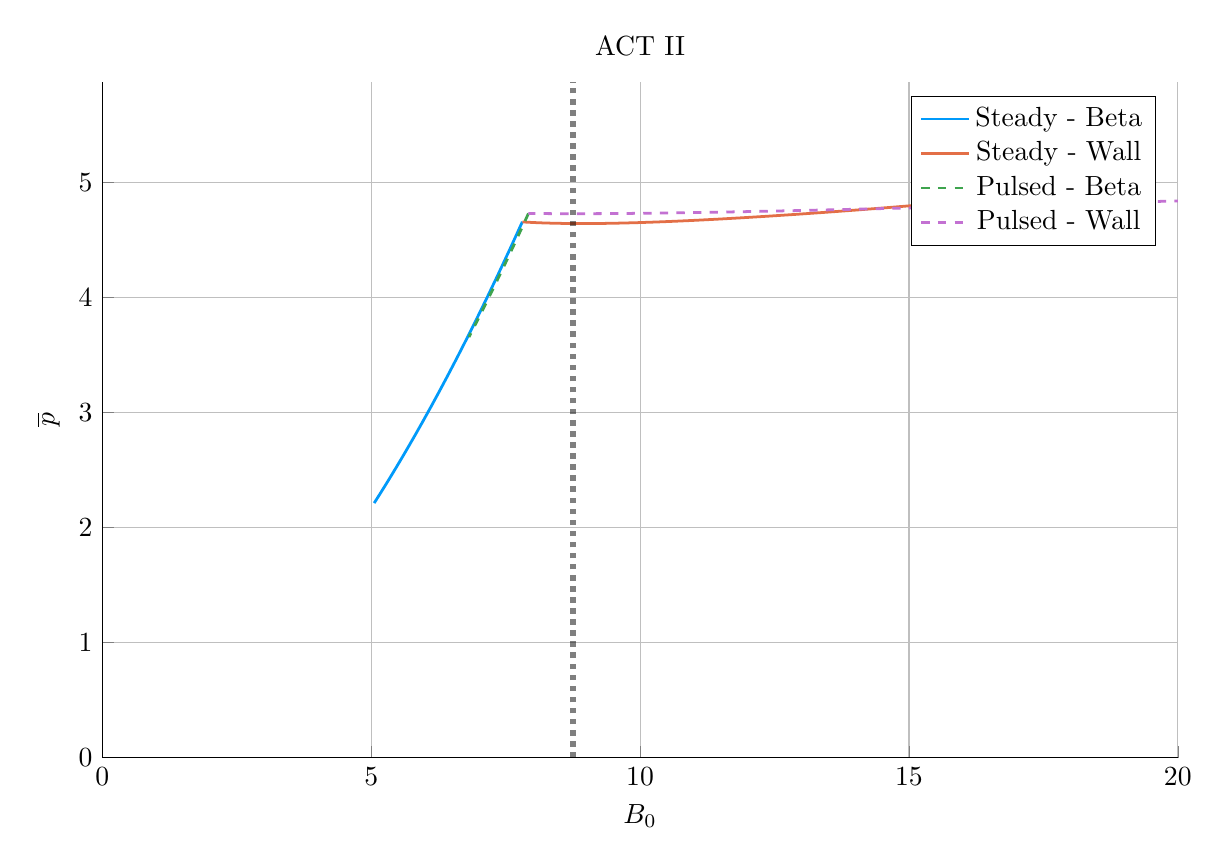
\begin{tikzpicture}[]
\begin{axis}[height = {101.6mm}, ylabel = {$\overline {p}$}, title = {ACT II}, xmin = {0.0}, xmax = {20.0}, ymax = {5.868693333369997}, xlabel = {${B}_{0}$}, {unbounded coords=jump, scaled x ticks = false, xticklabel style={rotate = 0}, xmajorgrids = true, xtick = {0.0,5.0,10.0,15.0,20.0}, xticklabels = {0,5,10,15,20}, xtick align = inside, axis lines* = left, scaled y ticks = false, yticklabel style={rotate = 0}, ymajorgrids = true, ytick = {0.0,1.0,2.0,3.0,4.0,5.0}, yticklabels = {0,1,2,3,4,5}, ytick align = inside, axis lines* = left,     xshift = 0.0mm,
    yshift = 0.0mm,
    axis background/.style={fill={rgb,1:red,1.00000000;green,1.00000000;blue,1.00000000}}
, colorbar style={title=}}, ymin = {0.0}, width = {152.4mm}]\addplot+ [color = {rgb,1:red,0.00000000;green,0.60560316;blue,0.97868012},
draw opacity=1.0,
line width=1,
solid,mark = none,
mark size = 2.0,
mark options = {
    color = {rgb,1:red,0.00000000;green,0.00000000;blue,0.00000000}, draw opacity = 1.0,
    fill = {rgb,1:red,0.00000000;green,0.60560316;blue,0.97868012}, fill opacity = 1.0,
    line width = 1,
    rotate = 0,
    solid
}]coordinates {
(7.810935944285959, 4.655957004843886)
(7.57736049850867, 4.416243026988451)
(7.354864292609041, 4.193518951706871)
(7.145167234136329, 3.988549147818302)
(6.9473303865083675, 3.7995817746750102)
(6.760499508614096, 3.625069666921968)
(6.583897990324067, 3.463644682023047)
(6.416817229618043, 3.3140927897245103)
(6.258609820663305, 3.1753343490701664)
(6.108683264880386, 3.0464069910140896)
(5.966494431410919, 2.926450956468271)
(5.831544666176381, 2.814696500005511)
(5.703375459679132, 2.710453033467129)
(5.581564609582325, 2.613099750491008)
(5.465722802994068, 2.522077498433624)
(5.355490573482678, 2.436881719809989)
(5.25053558682053, 2.357056307557123)
(5.1505502068221745, 2.282188236000175)
(5.0552493196883175, 2.211902868025681)
};
\addlegendentry{Steady - Beta}
\addplot+ [color = {rgb,1:red,0.88887350;green,0.43564919;blue,0.27812294},
draw opacity=1.0,
line width=1,
solid,mark = none,
mark size = 2.0,
mark options = {
    color = {rgb,1:red,0.00000000;green,0.00000000;blue,0.00000000}, draw opacity = 1.0,
    fill = {rgb,1:red,0.88887350;green,0.43564919;blue,0.27812294}, fill opacity = 1.0,
    line width = 1,
    rotate = 0,
    solid
}]coordinates {
(17.25550839059296, 4.890577777808331)
(16.594334962335296, 4.859208872930983)
(15.9071755430688, 4.829858662225014)
(15.233983138507648, 4.8029411060140195)
(14.594239858921854, 4.7786019588411905)
(13.989673082630297, 4.756710802422768)
(13.414782495717416, 4.737014906211031)
(12.872659546281994, 4.719449448527797)
(12.364365715508608, 4.703932731523149)
(11.889507953196574, 4.690370265982965)
(11.44685939646348, 4.678662275187154)
(11.034739998180656, 4.668708160689585)
(10.651252523287319, 4.660409179291977)
(10.294428800132035, 4.653670025466424)
(9.962319203963213, 4.648399726467713)
(9.653045819449929, 4.644512098653419)
(9.364832254395445, 4.641925921993596)
(9.096018465506306, 4.640564933980103)
(8.844373144802077, 4.640336403757336)
(8.61055754360846, 4.641237470592201)
(8.391192178573277, 4.643141856485801)
(8.18577947665566, 4.646012672315776)
(7.99323348423048, 4.6497956865424115)
(7.812301489248497, 4.654431182291782)
};
\addlegendentry{Steady - Wall}
\addplot+ [color = {rgb,1:red,0.24222430;green,0.64327509;blue,0.30444865},
draw opacity=1.0,
line width=1,
dashed,mark = none,
mark size = 2.0,
mark options = {
    color = {rgb,1:red,0.00000000;green,0.00000000;blue,0.00000000}, draw opacity = 1.0,
    fill = {rgb,1:red,0.24222430;green,0.64327509;blue,0.30444865}, fill opacity = 1.0,
    line width = 1,
    rotate = 0,
    solid
}]coordinates {
(7.923668284887995, 4.728016157875253)
(7.923668284887995, 4.72801615787525)
(7.836759696043437, 4.6388161703039135)
(7.6662731560983355, 4.466225553543672)
(7.50499428233835, 4.3058812264538515)
(7.35232773269976, 4.156730721437486)
(7.207727224738343, 4.017831507960247)
(7.070690693175276, 3.888337702441832)
(6.940756001029682, 3.7674885941428795)
(6.817497143644154, 3.6545987222271354)
};
\addlegendentry{Pulsed - Beta}
\addplot+ [color = {rgb,1:red,0.76444018;green,0.44411178;blue,0.82429754},
draw opacity=1.0,
line width=1,
dashed,mark = none,
mark size = 2.0,
mark options = {
    color = {rgb,1:red,0.00000000;green,0.00000000;blue,0.00000000}, draw opacity = 1.0,
    fill = {rgb,1:red,0.76444018;green,0.44411178;blue,0.82429754}, fill opacity = 1.0,
    line width = 1,
    rotate = 0,
    solid
}]coordinates {
(22.56106430311702, 4.868586689515289)
(20.85607192394036, 4.847634057308308)
(19.335265246056654, 4.828819929149097)
(17.974121547130903, 4.811994783401802)
(16.751976718553127, 4.797023120204419)
(15.651329744019142, 4.7837818789002275)
(14.65728744097675, 4.772159057658345)
(13.757118584462601, 4.762052510818542)
(12.939893642194303, 4.753368898213794)
(12.196191964860315, 4.746022764674995)
(11.517862472405039, 4.739935731394554)
(10.897827027335556, 4.735035783630904)
(10.329918077124672, 4.731256642143941)
(9.808743940706389, 4.728537206176256)
(9.329576544487265, 4.726821059993102)
(8.888257451278507, 4.726056033852692)
(8.481118883411932, 4.726193812923371)
(8.10491708701527, 4.727189588145797)
(7.923668284887995, 4.728016157875253)
(7.923668284887995, 4.72801615787525)
};
\addlegendentry{Pulsed - Wall}
\addplot+ [color = {rgb,1:red,0.00000000;green,0.00000000;blue,0.00000000},
draw opacity=0.5,
line width=2,
dotted,mark = none,
mark size = 2.0,
mark options = {
    color = {rgb,1:red,0.00000000;green,0.00000000;blue,0.00000000}, draw opacity = 0.5,
    fill = {rgb,1:red,0.00000000;green,0.00000000;blue,0.00000000}, fill opacity = 0.5,
    line width = 1,
    rotate = 0,
    solid
},forget plot]coordinates {
(0.0, NaN)
(20.0, NaN)
};
\addplot+ [color = {rgb,1:red,0.00000000;green,0.00000000;blue,0.00000000},
draw opacity=0.5,
line width=2,
dotted,mark = none,
mark size = 2.0,
mark options = {
    color = {rgb,1:red,0.00000000;green,0.00000000;blue,0.00000000}, draw opacity = 0.5,
    fill = {rgb,1:red,0.00000000;green,0.00000000;blue,0.00000000}, fill opacity = 0.5,
    line width = 1,
    rotate = 0,
    solid
},forget plot]coordinates {
(8.75, 0.0)
(8.75, 5.868693333369997)
};
\addplot+[draw=none, color = {rgb,1:red,0.00000000;green,0.00000000;blue,0.00000000},
draw opacity=0.5,
line width=0,
solid,mark = *,
mark size = 2.0,
mark options = {
    color = {rgb,1:red,0.00000000;green,0.00000000;blue,0.00000000}, draw opacity = 0.5,
    fill = {rgb,1:red,0.00000000;green,0.00000000;blue,0.00000000}, fill opacity = 0.5,
    line width = 1,
    rotate = 0,
    solid
},forget plot] coordinates {
(8.75, NaN)
};
\end{axis}

\end{tikzpicture}

    \end{adjustbox}
        \caption{ACT II}
    \end{subfigure}
    \hfill \hfill ~\\ ~\\ ~\\ ~\\
  \caption[]{Magnet Scan: $\overline p$ vs $B_0$} ~\\
\end{figure*}


\clearpage

\newpage

\subsection*{ Confinement Time -- $\tau_E$ }
  \label{subsection:scan_tau_E}

\begin{figure*}[h!]
    \centering
    \hfill
    \begin{subfigure}[t]{0.45\textwidth}
        \centering
    \begin{adjustbox}{width=\textwidth}
      \Large
      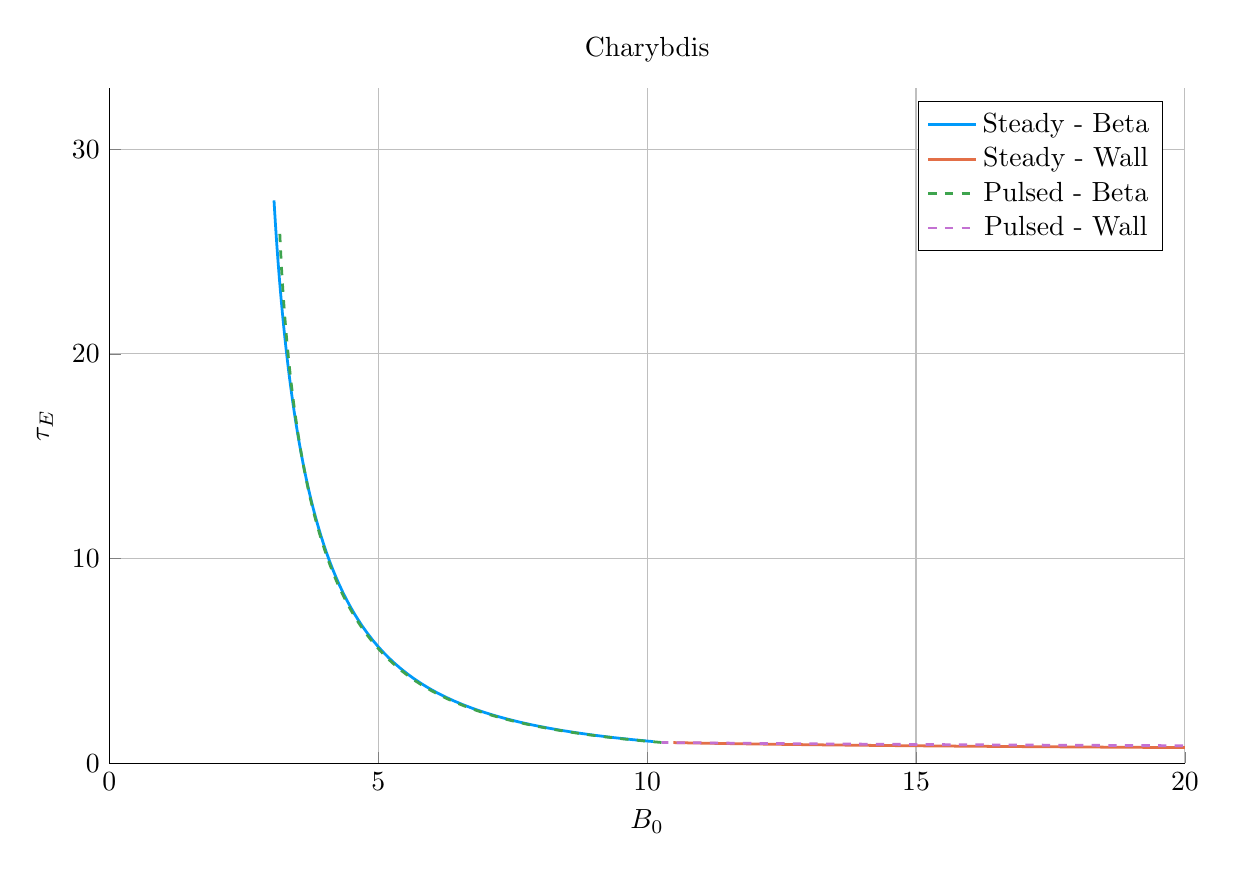
\begin{tikzpicture}[]
\begin{axis}[height = {101.6mm}, ylabel = {${\tau}_{E}$}, title = {Charybdis}, xmin = {0.0}, xmax = {20.0}, ymax = {32.99180627453526}, xlabel = {${B}_{0}$}, {unbounded coords=jump, scaled x ticks = false, xticklabel style={rotate = 0}, xmajorgrids = true, xtick = {0.0,5.0,10.0,15.0,20.0}, xticklabels = {0,5,10,15,20}, xtick align = inside, axis lines* = left, scaled y ticks = false, yticklabel style={rotate = 0}, ymajorgrids = true, ytick = {0.0,10.0,20.0,30.0}, yticklabels = {0,10,20,30}, ytick align = inside, axis lines* = left,     xshift = 0.0mm,
    yshift = 0.0mm,
    axis background/.style={fill={rgb,1:red,1.00000000;green,1.00000000;blue,1.00000000}}
, colorbar style={title=}}, ymin = {0.0}, width = {152.4mm}]\addplot+ [color = {rgb,1:red,0.00000000;green,0.60560316;blue,0.97868012},
draw opacity=1.0,
line width=1,
solid,mark = none,
mark size = 2.0,
mark options = {
    color = {rgb,1:red,0.00000000;green,0.00000000;blue,0.00000000}, draw opacity = 1.0,
    fill = {rgb,1:red,0.00000000;green,0.60560316;blue,0.97868012}, fill opacity = 1.0,
    line width = 1,
    rotate = 0,
    solid
}]coordinates {
(10.112818033153026, 1.0625161517384192)
(9.722156888543116, 1.1594988678345357)
(9.357875603858393, 1.2626839305987037)
(9.017653755630063, 1.3722801867221375)
(8.6995124437054, 1.4884677556178918)
(8.401566530516865, 1.6114513083009556)
(8.122163706328223, 1.7414206902158769)
(7.859819415455661, 1.8785597400470764)
(7.613196557650265, 2.0230457662487638)
(7.381088038653343, 2.1750490464895056)
(7.162401716104116, 2.3347323517053176)
(6.956147367527331, 2.5022504962769663)
(6.761425371986388, 2.6777499156649123)
(6.577416849463348, 2.861368272654205)
(6.403375044688587, 3.053234093181537)
(6.2386177769852695, 3.2534664325373566)
(6.0825208065966905, 3.462174572303039)
(5.934511989185341, 3.6794577500291927)
(5.794066116682695, 3.905404918060345)
(5.660700347012839, 4.140094536782916)
(5.533970150598111, 4.383594398430443)
(5.413465705416883, 4.635961483032188)
(5.298808685607224, 4.897241844565363)
(5.189649392059402, 5.167470530402597)
(5.085664187259174, 5.446671528743596)
(4.986553195072601, 5.734857746990561)
(4.892038235455667, 6.032031018850494)
(4.801860966679364, 6.338182139561831)
(4.7157812114040425, 6.653290928317218)
(4.633575445956479, 6.977326316879843)
(4.5550354347559185, 7.3102464633285065)
(4.479966994069385, 7.651998889809481)
(4.408188871204256, 8.00252064312815)
(4.33953172691477, 8.361738476973796)
(4.273837210246432, 8.7295690545395)
(4.210957116299974, 9.10591917027589)
(4.15075261849161, 9.490685989502143)
(4.0930935678432965, 9.883757304586293)
(4.037857852672517, 10.285011806404352)
(3.9849308127842145, 10.694319369789481)
(3.9342047029103653, 11.111541351692367)
(3.8855782007091695, 11.53653090078437)
(3.838955955133626, 11.969133277254734)
(3.7942481714200484, 12.409186181573288)
(3.7513702293348077, 12.856520091020052)
(3.710242331663442, 13.310958602806018)
(3.6707891802306123, 13.7723187826474)
(3.6329396770109583, 14.240411517689399)
(3.5966266481325166, 14.715041872710676)
(3.5617865887889004, 15.196009448583396)
(3.5283594272686503, 15.683108742000226)
(3.496288306480746, 16.176129505529673)
(3.465519381509793, 16.67485710709366)
(3.4360016318699595, 17.179072888019583)
(3.4076866872513096, 17.6885545188531)
(3.380528665662031, 18.20307635216785)
(3.3544840229690007, 18.722409771658352)
(3.3295114129297314, 19.24632353683724)
(3.3055715568879336, 19.774584122716096)
(3.2826271223788512, 20.306956053882768)
(3.260642607548369, 20.843202254844744)
(3.239584247604666, 21.383084259315513)
(3.2194198921826622, 21.926362748475)
(3.2001189373344725, 22.472797633654757)
(3.181652227422265, 23.02214846722306)
(3.163991977015565, 23.57417471084791)
(3.1471116955378684, 24.12863601768145)
(3.130986116696265, 24.685292505804554)
(3.115591132350856, 25.24390502271186)
(3.1009037305081053, 25.804235400653166)
(3.0869019371473265, 26.366046702679103)
(3.0735647616124355, 26.929103459268216)
(3.0608721453218655, 27.493171895446046)
};
\addlegendentry{Steady - Beta}
\addplot+ [color = {rgb,1:red,0.88887350;green,0.43564919;blue,0.27812294},
draw opacity=1.0,
line width=1,
solid,mark = none,
mark size = 2.0,
mark options = {
    color = {rgb,1:red,0.00000000;green,0.00000000;blue,0.00000000}, draw opacity = 1.0,
    fill = {rgb,1:red,0.88887350;green,0.43564919;blue,0.27812294}, fill opacity = 1.0,
    line width = 1,
    rotate = 0,
    solid
}]coordinates {
(20.758867641064707, 0.7513738330624348)
(20.346250098246923, 0.7623932074222438)
(19.57104597888471, 0.7750238546968216)
(18.681781921115476, 0.788717059315887)
(17.775790175980152, 0.8032229934578131)
(16.896654716492492, 0.8183968657895727)
(16.063927450323227, 0.8341438062685621)
(15.285557510665852, 0.8503960522346193)
(14.563500533069154, 0.867102604925121)
(13.896568848875791, 0.8842236990605942)
(13.281970890030232, 0.9017275241394246)
(12.716170469467318, 0.9195881307840134)
(12.195372283741088, 0.9377840185416357)
(11.715794270833433, 0.9562971430632552)
(11.273815669498969, 0.9751121952773113)
(10.866051794088186, 0.9942160644439935)
(10.489365023931143, 1.0135975466150031)
};
\addlegendentry{Steady - Wall}
\addplot+ [color = {rgb,1:red,0.24222430;green,0.64327509;blue,0.30444865},
draw opacity=1.0,
line width=1,
dashed,mark = none,
mark size = 2.0,
mark options = {
    color = {rgb,1:red,0.00000000;green,0.00000000;blue,0.00000000}, draw opacity = 1.0,
    fill = {rgb,1:red,0.24222430;green,0.64327509;blue,0.30444865}, fill opacity = 1.0,
    line width = 1,
    rotate = 0,
    solid
}]coordinates {
(10.26788634689966, 1.0190112167421927)
(9.953967652326213, 1.091110478427649)
(9.567926244368271, 1.1910195193315796)
(9.207974394987358, 1.2973518320169073)
(8.871841888699304, 1.4103195545362353)
(8.557505525932248, 1.5301291155727108)
(8.263156925406376, 1.656980416297674)
(7.9871752024348766, 1.7910660261526372)
(7.728103682045175, 1.9325703985634266)
(7.484629973620137, 2.0816691106390905)
(7.255568856523303, 2.23852813133106)
(7.039847526735421, 2.4033031222337597)
(6.836492834698909, 2.5761387749617124)
(6.644620209081183, 2.7571681887573685)
(6.463424013335149, 2.9465122916736917)
(6.2921691243175495, 3.1442793083396894)
(6.13018355681404, 3.3505642769586483)
(5.97685198655569, 3.5654486174804063)
(5.831610044919842, 3.7889997548095593)
(5.693939286027163, 4.021270793608104)
(5.563362729090489, 4.262300252303879)
(5.439440906144732, 4.51211185211047)
(5.321768347746793, 4.770714363559232)
(5.209970453003084, 5.038101508321995)
(5.103700692769835, 5.314251920363263)
(5.002638109938164, 5.5991291594262105)
(4.906485077678376, 5.892681780300472)
(4.814965286571576, 6.194843454462518)
(4.727821933804548, 6.505533142575857)
(4.644816091323922, 6.824655315753062)
(4.565725232806084, 7.15210022323614)
(4.490341901840154, 7.487744203940372)
(4.418472505906755, 7.831450039125086)
(4.349936222622964, 8.183067343300472)
(4.284564006352339, 8.542432990364109)
(4.222197684694192, 8.909371571866613)
(4.162689135592264, 9.283695884250033)
(4.105899536872315, 9.665207441869741)
(4.051698680949713, 10.053697012608831)
(3.9999643482627323, 10.44894517291684)
(3.9505817337017928, 10.850722879147153)
(3.903442920928527, 11.2587920521459)
(3.858446400032002, 11.672906172121287)
(3.8154966244515616, 12.092810880938382)
(3.7745036035252744, 12.518244589098753)
(3.7353825273991994, 12.948939084805462)
(3.6980534213689746, 13.384620142651396)
(3.6624408270205375, 13.825008129628543)
(3.62847350780097, 14.269818606312347)
(3.5960841768845415, 14.71876292123903)
(3.565209245407392, 15.171548796664778)
(3.5357885893311605, 15.627880904054313)
(3.5077653333614305, 16.0874614278211)
(3.4810856504959875, 16.549990615998112)
(3.4556985759109375, 17.01516731668133)
(3.4315558340122845, 17.482689499239914)
(3.408611677587535, 17.952254759438645)
(3.3868227380888998, 18.423560807754622)
(3.36614788616562, 18.8963059403109)
(3.3465481016421226, 19.370189491967345)
(3.327986352208224, 19.844912271235764)
(3.3104274769652595, 20.32017700628081)
(3.2938380965241474, 20.79568859542677)
(3.278186482171801, 21.27115478148464)
(3.263442495132517, 21.746286217693427)
(3.2495774839156075, 22.220796957642932)
(3.236564206241785, 22.69440475001181)
(3.224376752844934, 23.16683134481192)
(3.212990475972638, 23.637802781937474)
(3.2023819222517877, 24.10704966234626)
(3.192528769611062, 24.574307402247662)
(3.1834097679780142, 25.039316470685087)
(3.1750046834890777, 25.50182261093869)
(3.1672942459724482, 25.961577046178377)
};
\addlegendentry{Pulsed - Beta}
\addplot+ [color = {rgb,1:red,0.76444018;green,0.44411178;blue,0.82429754},
draw opacity=1.0,
line width=1,
dashed,mark = none,
mark size = 2.0,
mark options = {
    color = {rgb,1:red,0.00000000;green,0.00000000;blue,0.00000000}, draw opacity = 1.0,
    fill = {rgb,1:red,0.76444018;green,0.44411178;blue,0.82429754}, fill opacity = 1.0,
    line width = 1,
    rotate = 0,
    solid
}]coordinates {
(48.990476413653056, 0.7236146731172175)
(42.83950920694117, 0.7398265310143234)
(37.687790427214495, 0.7565896148522706)
(33.33937742845888, 0.773869376245486)
(29.64296398154308, 0.7916362945827186)
(26.48039367255613, 0.8098649456001076)
(23.758442882319894, 0.8285332680712999)
(21.402860298405816, 0.8476219814334762)
(19.353987387634486, 0.8671141195298459)
(17.563502020363714, 0.8869946544854104)
(15.991970371213752, 0.9072501911761787)
(14.606987499719377, 0.9278687173826333)
(13.381751501116137, 0.9488393982412359)
(12.293960329570087, 0.9701524061610466)
(11.32495111804522, 0.9917987793304357)
(10.459023415380802, 1.013770303415277)
(10.26788634689966, 1.0190112167421927)
};
\addlegendentry{Pulsed - Wall}
\end{axis}

\end{tikzpicture}

    \end{adjustbox}
        \caption{Charybdis}
    \end{subfigure}
    \hfill
    \begin{subfigure}[t]{0.45\textwidth}
        \centering
    \begin{adjustbox}{width=\textwidth}
      \Large
      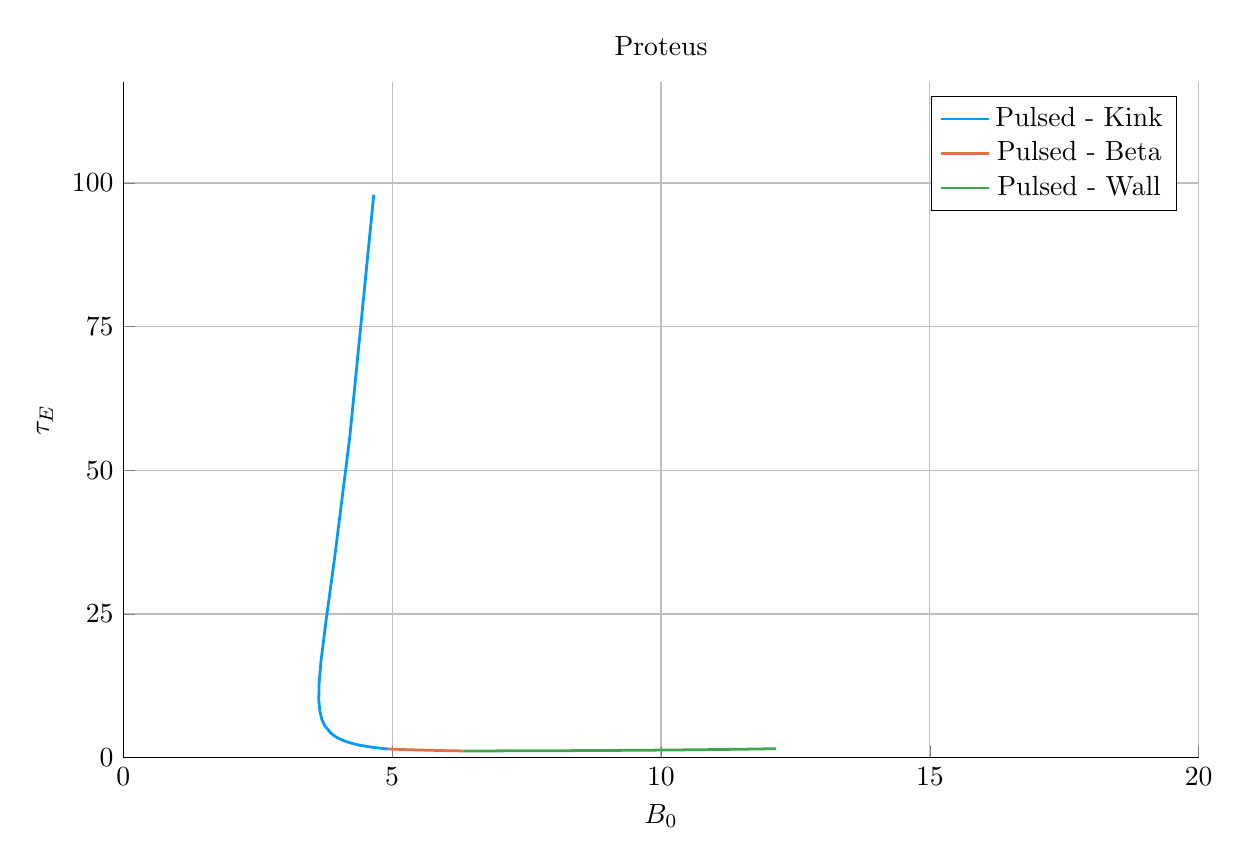
\begin{tikzpicture}[]
\begin{axis}[height = {101.6mm}, ylabel = {${\tau}_{E}$}, title = {Proteus}, xmin = {0.0}, xmax = {20.0}, ymax = {117.54114307770362}, xlabel = {${B}_{0}$}, {unbounded coords=jump, scaled x ticks = false, xticklabel style={rotate = 0}, xmajorgrids = true, xtick = {0.0,5.0,10.0,15.0,20.0}, xticklabels = {0,5,10,15,20}, xtick align = inside, axis lines* = left, scaled y ticks = false, yticklabel style={rotate = 0}, ymajorgrids = true, ytick = {0.0,25.0,50.0,75.0,100.0}, yticklabels = {0,25,50,75,100}, ytick align = inside, axis lines* = left,     xshift = 0.0mm,
    yshift = 0.0mm,
    axis background/.style={fill={rgb,1:red,1.00000000;green,1.00000000;blue,1.00000000}}
, colorbar style={title=}}, ymin = {0.0}, width = {152.4mm}]\addplot+ [color = {rgb,1:red,0.00000000;green,0.60560316;blue,0.97868012},
draw opacity=1.0,
line width=1,
solid,mark = none,
mark size = 2.0,
mark options = {
    color = {rgb,1:red,0.00000000;green,0.00000000;blue,0.00000000}, draw opacity = 1.0,
    fill = {rgb,1:red,0.00000000;green,0.60560316;blue,0.97868012}, fill opacity = 1.0,
    line width = 1,
    rotate = 0,
    solid
}]coordinates {
(4.658732060637907, 97.95095256475302)
(4.211109766361548, 55.66859437434958)
(3.9293920326356777, 34.684315066530935)
(3.7651903683456465, 23.414521469687102)
(3.6776039543745567, 16.83124979368127)
(3.6402437753208394, 12.70108728618661)
(3.6366994671255806, 9.95566301325721)
(3.656621534643579, 8.043577750881989)
(3.693300156736026, 6.660408400940047)
(3.7422515017241134, 5.628123437056208)
(3.865532743079537, 4.218264736499625)
(3.936096932264377, 3.7243162927716376)
(4.010907188015084, 3.3238303715392066)
(4.089072356933184, 2.9945356894831514)
(4.169903401491354, 2.720430778637335)
(4.252857906625248, 2.4897818684440622)
(4.337501757261618, 2.2938274549015176)
(4.42348218754058, 2.125918783302953)
(4.5983381267510195, 1.8548872722012077)
(4.686766232902671, 1.7446180388447472)
(4.775618142770625, 1.6476127932688729)
(4.864743502376605, 1.5618435004492102)
(4.927312314219091, 1.5075203195512064)
};
\addlegendentry{Pulsed - Kink}
\addplot+ [color = {rgb,1:red,0.88887350;green,0.43564919;blue,0.27812294},
draw opacity=1.0,
line width=1,
solid,mark = none,
mark size = 2.0,
mark options = {
    color = {rgb,1:red,0.00000000;green,0.00000000;blue,0.00000000}, draw opacity = 1.0,
    fill = {rgb,1:red,0.88887350;green,0.43564919;blue,0.27812294}, fill opacity = 1.0,
    line width = 1,
    rotate = 0,
    solid
}]coordinates {
(4.927312314219091, 1.5075203195512064)
(4.984545814413324, 1.487546126853633)
(5.17452482724068, 1.4258573261241823)
(5.362091669637646, 1.3712392041536523)
(5.54700293215903, 1.3227859198350533)
(5.729042482638278, 1.2797342709066928)
(5.908022832274664, 1.2414369624246038)
(6.083785777786694, 1.207341630243464)
(6.256202341425288, 1.1769742503887919)
(6.324169421042356, 1.1657839175752975)
};
\addlegendentry{Pulsed - Beta}
\addplot+ [color = {rgb,1:red,0.24222430;green,0.64327509;blue,0.30444865},
draw opacity=1.0,
line width=1,
solid,mark = none,
mark size = 2.0,
mark options = {
    color = {rgb,1:red,0.00000000;green,0.00000000;blue,0.00000000}, draw opacity = 1.0,
    fill = {rgb,1:red,0.24222430;green,0.64327509;blue,0.30444865}, fill opacity = 1.0,
    line width = 1,
    rotate = 0,
    solid
}]coordinates {
(6.324169421042356, 1.1657839175752975)
(6.727338549778396, 1.173574607212312)
(7.320469048424473, 1.1880230460869503)
(7.835746509376305, 1.2038714296520943)
(8.290245520072391, 1.2207982334225753)
(8.696162676727877, 1.2385974280252556)
(9.0624397222742, 1.2571294388176562)
(9.395798186463841, 1.2762953061659403)
(9.701405747258567, 1.2960221858655594)
(10.244760202900984, 1.3369499159457439)
(10.930275827723788, 1.40149804218626)
(11.131878682735255, 1.4237571536892408)
(11.50278450645086, 1.4692867854332288)
(11.83715172742864, 1.516081213501197)
(11.992609772603878, 1.5399272456612312)
(12.141110720831467, 1.5640613260055054)
};
\addlegendentry{Pulsed - Wall}
\end{axis}

\end{tikzpicture}

    \end{adjustbox}
        \caption{Proteus}
    \end{subfigure}
    \hfill \hfill ~\\ ~\\ ~\\ ~\\
    \hfill
    \begin{subfigure}[t]{0.45\textwidth}
        \centering
    \begin{adjustbox}{width=\textwidth}
      \Large
      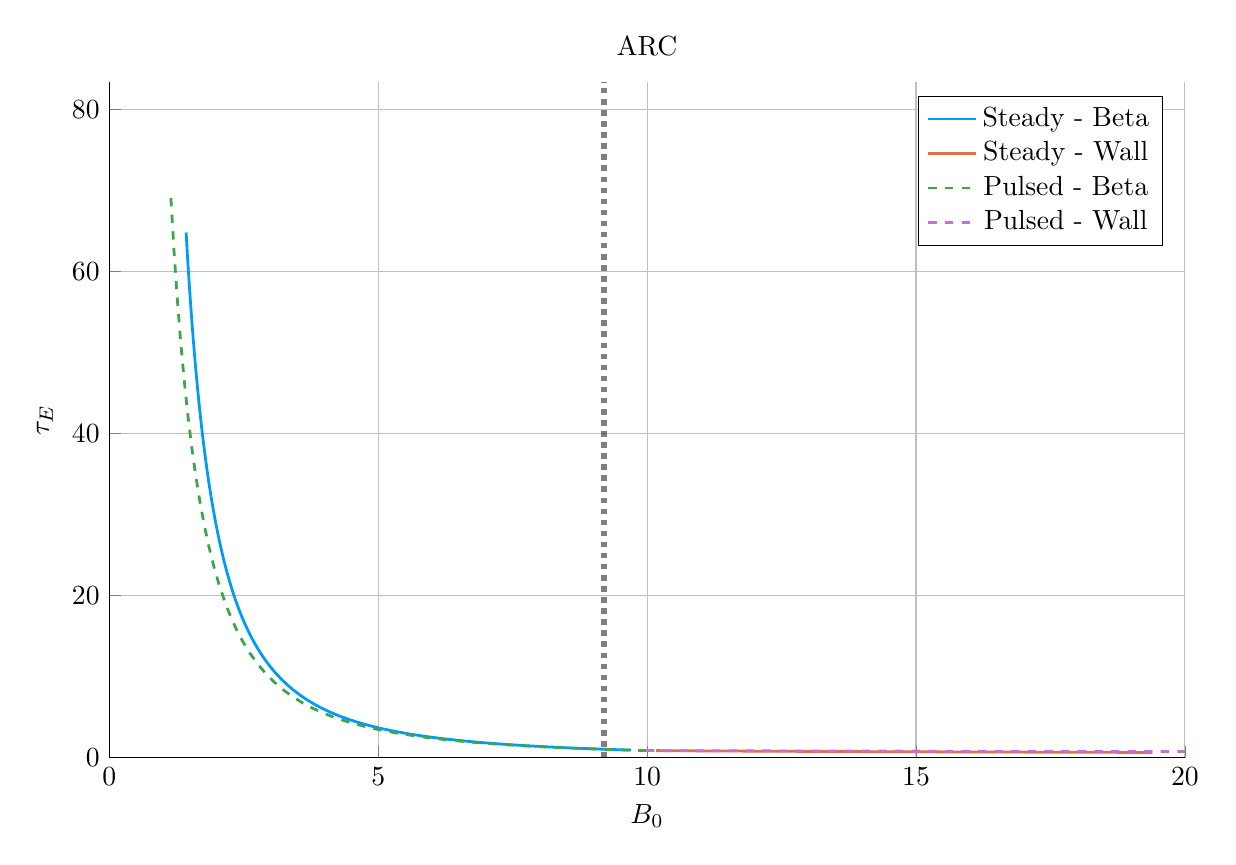
\begin{tikzpicture}[]
\begin{axis}[height = {101.6mm}, ylabel = {${\tau}_{E}$}, title = {ARC}, xmin = {0.0}, xmax = {20.0}, ymax = {83.36141561369563}, xlabel = {${B}_{0}$}, {unbounded coords=jump, scaled x ticks = false, xticklabel style={rotate = 0}, xmajorgrids = true, xtick = {0.0,5.0,10.0,15.0,20.0}, xticklabels = {0,5,10,15,20}, xtick align = inside, axis lines* = left, scaled y ticks = false, yticklabel style={rotate = 0}, ymajorgrids = true, ytick = {0.0,20.0,40.0,60.0,80.0}, yticklabels = {0,20,40,60,80}, ytick align = inside, axis lines* = left,     xshift = 0.0mm,
    yshift = 0.0mm,
    axis background/.style={fill={rgb,1:red,1.00000000;green,1.00000000;blue,1.00000000}}
, colorbar style={title=}}, ymin = {0.0}, width = {152.4mm}]\addplot+ [color = {rgb,1:red,0.00000000;green,0.60560316;blue,0.97868012},
draw opacity=1.0,
line width=1,
solid,mark = none,
mark size = 2.0,
mark options = {
    color = {rgb,1:red,0.00000000;green,0.00000000;blue,0.00000000}, draw opacity = 1.0,
    fill = {rgb,1:red,0.00000000;green,0.60560316;blue,0.97868012}, fill opacity = 1.0,
    line width = 1,
    rotate = 0,
    solid
}]coordinates {
(9.701206080853105, 0.9327083734907325)
(9.162315904693079, 1.047631316713215)
(8.664301107137337, 1.1741459302569808)
(8.203576462497304, 1.3130944385509704)
(7.776718537485166, 1.4654047476296803)
(7.380720231870917, 1.6320314598864853)
(7.012886014999712, 1.8139671221489049)
(6.670795005901889, 2.012241401342966)
(6.352268997292712, 2.227920078401859)
(6.055344682097163, 2.462103860548695)
(5.778249464564785, 2.7159270132190425)
(5.519380338856715, 2.990555814015613)
(5.2772854007125325, 3.287186832192051)
(5.050647625972996, 3.6070450382372963)
(4.838270606140816, 3.951381749169139)
(4.639065978019038, 4.321472416133619)
(4.4520423235376105, 4.718614261841429)
(4.276295348572609, 5.144123776247871)
(4.110999177018484, 5.599334079687999)
(3.9553986195015125, 6.08559216341556)
(3.8088022956698633, 6.604256018153765)
(3.6705765055641186, 7.156691661847382)
(3.54013975965751, 7.7442700783054335)
(3.4169578891619192, 8.368364078841708)
(3.30053966845824, 9.030345099353319)
(3.1904328903033052, 9.731579945530608)
(3.086220842019516, 10.473427499057426)
(2.9875191373772063, 11.257235397749337)
(2.8939728644914635, 12.08433670258646)
(2.8052540149097247, 12.956046564527512)
(2.7210591632720242, 13.87365890385172)
(2.6411073705789065, 14.838443114563244)
(2.565138287279709, 15.851640806116942)
(2.492910435164382, 16.914462594384766)
(2.4241996494611984, 18.02808495338735)
(2.3587976646588236, 19.19364713886711)
(2.296510829425685, 20.4122481942879)
(2.237158937627476, 21.684944049302498)
(2.180574163874242, 23.01274472016261)
(2.126600093288366, 24.396611620933967)
(2.075090836295778, 25.83745499374929)
(2.0259102202234582, 27.33613146567406)
(1.978931050353818, 28.893441739087702)
(1.9340344338545452, 30.51012842180039)
(1.8911091606836798, 32.186874002424304)
(1.8500511361739687, 33.924298975832)
(1.8107628605384507, 35.72296012282494)
(1.773152951016952, 37.58334894745847)
(1.7371357028100902, 39.505890274764134)
(1.7026306853269466, 41.49094101095818)
(1.6695623706125668, 43.538789067551086)
(1.6378597911249178, 45.64965245013732)
(1.607456224302725, 47.82367851202235)
(1.5782889016090462, 50.06094337224119)
(1.5502987399539199, 52.361451496953585)
(1.5234300935954943, 54.7251354426418)
(1.4976305247952577, 57.1518557590222)
(1.4728505916614916, 59.64140104908817)
(1.4490436517578602, 62.19348818323689)
(1.4261656801829077, 64.80776266398635)
};
\addlegendentry{Steady - Beta}
\addplot+ [color = {rgb,1:red,0.88887350;green,0.43564919;blue,0.27812294},
draw opacity=1.0,
line width=1,
solid,mark = none,
mark size = 2.0,
mark options = {
    color = {rgb,1:red,0.00000000;green,0.00000000;blue,0.00000000}, draw opacity = 1.0,
    fill = {rgb,1:red,0.88887350;green,0.43564919;blue,0.27812294}, fill opacity = 1.0,
    line width = 1,
    rotate = 0,
    solid
}]coordinates {
(19.394007482712425, 0.6389760209182812)
(18.932196567189358, 0.650080623527837)
(18.296989378345195, 0.6620076068230863)
(17.587029315408756, 0.6745667061677622)
(16.847882407994106, 0.6876614720651362)
(16.111374502564406, 0.7012135164758136)
(15.396027314547156, 0.7151659968990569)
(14.710952688793137, 0.7294797531179514)
(14.06168447794857, 0.7441215586048141)
(13.450465418483889, 0.7590653540262556)
(12.877644538645335, 0.7742898692181243)
(12.342394470642008, 0.7897775055382761)
(11.843182246608265, 0.8055135380143609)
(11.376441269625893, 0.8214924840664242)
(10.944966372727551, 0.8376828788375057)
(10.541663878705513, 0.8540964969661428)
(10.165908182236457, 0.8707190796770249)
};
\addlegendentry{Steady - Wall}
\addplot+ [color = {rgb,1:red,0.24222430;green,0.64327509;blue,0.30444865},
draw opacity=1.0,
line width=1,
dashed,mark = none,
mark size = 2.0,
mark options = {
    color = {rgb,1:red,0.00000000;green,0.00000000;blue,0.00000000}, draw opacity = 1.0,
    fill = {rgb,1:red,0.24222430;green,0.64327509;blue,0.30444865}, fill opacity = 1.0,
    line width = 1,
    rotate = 0,
    solid
}]coordinates {
(9.980483622051658, 0.8730418322159563)
(9.392786903460065, 0.9846456668946276)
(8.79273598103983, 1.122534670823961)
(8.23820290909994, 1.2777779252308081)
(7.725182218401588, 1.4523203419822088)
(7.250078106370205, 1.6482957960553868)
(6.80965553466646, 1.8680421351603016)
(6.400998063035608, 2.1141170503488462)
(6.0214713600430425, 2.3893148438573837)
(5.668691517461799, 2.696684140227185)
(5.340497445229901, 3.0395466013059447)
(5.034926745580058, 3.421516726638964)
(4.750194564008521, 3.846522850030527)
(4.484674995755211, 4.318829483254335)
(4.236884692979903, 4.843061212267565)
(4.00546837264544, 5.424228423967811)
(3.7891859704718387, 6.067755237800374)
(3.5869012239550364, 6.779510143156531)
(3.3975714987448393, 7.565840009281778)
(3.2202386987489797, 8.43360835085483)
(3.0540211220494466, 9.390239014789751)
(2.8981061427709687, 10.443766822753409)
(2.7517436139566023, 11.60289718760338)
(2.6142398986781377, 12.877077359727055)
(2.4849524463010138, 14.276582806833861)
(2.363284838174807, 15.812623368494105)
(2.248682232019848, 17.49747537275982)
(2.140627136740878, 19.344648033264686)
(2.038635448877246, 21.369095430815047)
(1.9422526775794744, 23.58748964304901)
(1.8510502754751532, 26.018576786019068)
(1.7646219756564088, 28.68364695806701)
(1.6825800061969869, 31.607163143228753)
(1.6045510059627948, 34.81761616115258)
(1.53017138625397, 38.348708299909795)
(1.4590817483192686, 42.241027610016125)
(1.3909197311384796, 46.544477816226326)
(1.3253102336217724, 51.32191576076217)
(1.261851128383913, 56.65480634511549)
(1.20009089049112, 62.65243634075118)
(1.1394908096975784, 69.46784634474636)
};
\addlegendentry{Pulsed - Beta}
\addplot+ [color = {rgb,1:red,0.76444018;green,0.44411178;blue,0.82429754},
draw opacity=1.0,
line width=1,
dashed,mark = none,
mark size = 2.0,
mark options = {
    color = {rgb,1:red,0.00000000;green,0.00000000;blue,0.00000000}, draw opacity = 1.0,
    fill = {rgb,1:red,0.76444018;green,0.44411178;blue,0.82429754}, fill opacity = 1.0,
    line width = 1,
    rotate = 0,
    solid
}]coordinates {
(29.27715761652869, 0.7126569714915048)
(25.4410619834368, 0.7311036273576099)
(22.158819835998365, 0.7499428117575023)
(19.342453256965573, 0.7691712949120021)
(16.919364280634177, 0.7887862917418604)
(14.829378672669455, 0.808785393262606)
(13.022412368922526, 0.8291665079461672)
(11.456617692058645, 0.8499278113153294)
(10.096901921254785, 0.8710677023807946)
(9.980483622051658, 0.8730418322159563)
};
\addlegendentry{Pulsed - Wall}
\addplot+ [color = {rgb,1:red,0.00000000;green,0.00000000;blue,0.00000000},
draw opacity=0.5,
line width=2,
dotted,mark = none,
mark size = 2.0,
mark options = {
    color = {rgb,1:red,0.00000000;green,0.00000000;blue,0.00000000}, draw opacity = 0.5,
    fill = {rgb,1:red,0.00000000;green,0.00000000;blue,0.00000000}, fill opacity = 0.5,
    line width = 1,
    rotate = 0,
    solid
},forget plot]coordinates {
(0.0, NaN)
(20.0, NaN)
};
\addplot+ [color = {rgb,1:red,0.00000000;green,0.00000000;blue,0.00000000},
draw opacity=0.5,
line width=2,
dotted,mark = none,
mark size = 2.0,
mark options = {
    color = {rgb,1:red,0.00000000;green,0.00000000;blue,0.00000000}, draw opacity = 0.5,
    fill = {rgb,1:red,0.00000000;green,0.00000000;blue,0.00000000}, fill opacity = 0.5,
    line width = 1,
    rotate = 0,
    solid
},forget plot]coordinates {
(9.2, 0.0)
(9.2, 83.36141561369563)
};
\addplot+[draw=none, color = {rgb,1:red,0.00000000;green,0.00000000;blue,0.00000000},
draw opacity=0.5,
line width=0,
solid,mark = *,
mark size = 2.0,
mark options = {
    color = {rgb,1:red,0.00000000;green,0.00000000;blue,0.00000000}, draw opacity = 0.5,
    fill = {rgb,1:red,0.00000000;green,0.00000000;blue,0.00000000}, fill opacity = 0.5,
    line width = 1,
    rotate = 0,
    solid
},forget plot] coordinates {
(9.2, NaN)
};
\end{axis}

\end{tikzpicture}

    \end{adjustbox}
        \caption{ARC}
    \end{subfigure}
    \hfill
    \begin{subfigure}[t]{0.45\textwidth}
        \centering
    \begin{adjustbox}{width=\textwidth}
      \Large
      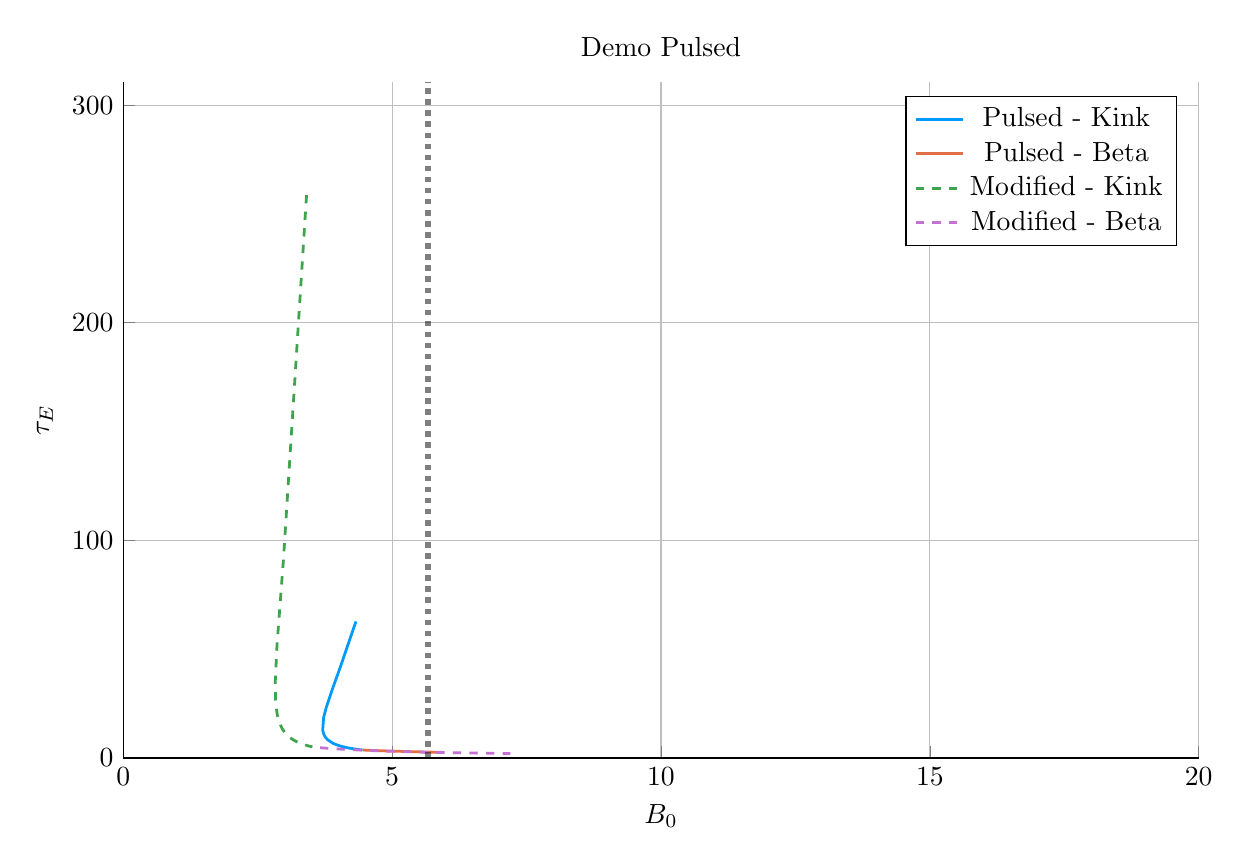
\begin{tikzpicture}[]
\begin{axis}[height = {101.6mm}, ylabel = {${\tau}_{E}$}, title = {Demo Pulsed}, xmin = {0.0}, xmax = {20.0}, ymax = {310.3939223459952}, xlabel = {${B}_{0}$}, {unbounded coords=jump, scaled x ticks = false, xticklabel style={rotate = 0}, xmajorgrids = true, xtick = {0.0,5.0,10.0,15.0,20.0}, xticklabels = {0,5,10,15,20}, xtick align = inside, axis lines* = left, scaled y ticks = false, yticklabel style={rotate = 0}, ymajorgrids = true, ytick = {0.0,100.0,200.0,300.0}, yticklabels = {0,100,200,300}, ytick align = inside, axis lines* = left,     xshift = 0.0mm,
    yshift = 0.0mm,
    axis background/.style={fill={rgb,1:red,1.00000000;green,1.00000000;blue,1.00000000}}
, colorbar style={title=}}, ymin = {0.0}, width = {152.4mm}]\addplot+ [color = {rgb,1:red,0.00000000;green,0.60560316;blue,0.97868012},
draw opacity=1.0,
line width=1,
solid,mark = none,
mark size = 2.0,
mark options = {
    color = {rgb,1:red,0.00000000;green,0.00000000;blue,0.00000000}, draw opacity = 1.0,
    fill = {rgb,1:red,0.00000000;green,0.60560316;blue,0.97868012}, fill opacity = 1.0,
    line width = 1,
    rotate = 0,
    solid
}]coordinates {
(4.327031075670194, 62.73471113745037)
(4.038214026054326, 41.89539888286328)
(3.8713719163129245, 30.375414501167093)
(3.7758613845615545, 23.269913963977316)
(3.7257856761317214, 18.546199772925064)
(3.7090473695925437, 12.801297001291132)
(3.727711597554826, 10.964235165501899)
(3.7586131667481433, 9.536799251127631)
(3.799052518631718, 8.402931788651731)
(3.901290136389271, 6.731129539626641)
(3.960577465316514, 6.102535653215946)
(4.0241209645210345, 5.572423403498513)
(4.0912717805663785, 5.120668831666732)
(4.161514602943343, 4.732110160552255)
(4.2344343960723005, 4.395137186268533)
(4.309692554546368, 4.100729716351705)
(4.450417240491067, 3.6556940720800073)
};
\addlegendentry{Pulsed - Kink}
\addplot+ [color = {rgb,1:red,0.88887350;green,0.43564919;blue,0.27812294},
draw opacity=1.0,
line width=1,
solid,mark = none,
mark size = 2.0,
mark options = {
    color = {rgb,1:red,0.00000000;green,0.00000000;blue,0.00000000}, draw opacity = 1.0,
    fill = {rgb,1:red,0.88887350;green,0.43564919;blue,0.27812294}, fill opacity = 1.0,
    line width = 1,
    rotate = 0,
    solid
}]coordinates {
(4.450417240491067, 3.6556940720800073)
(4.490148631384312, 3.613798203276785)
(4.692490181445514, 3.4154457886494347)
(4.8960344619053355, 3.238302829916966)
(5.100651132702229, 3.079437608144942)
(5.306202822090688, 2.9364242483314107)
(5.512545696627038, 2.807240473700629)
(5.719530043226767, 2.690188815147256)
(5.927000883375481, 2.583835289249025)
};
\addlegendentry{Pulsed - Beta}
\addplot+ [color = {rgb,1:red,0.24222430;green,0.64327509;blue,0.30444865},
draw opacity=1.0,
line width=1,
dashed,mark = none,
mark size = 2.0,
mark options = {
    color = {rgb,1:red,0.00000000;green,0.00000000;blue,0.00000000}, draw opacity = 1.0,
    fill = {rgb,1:red,0.24222430;green,0.64327509;blue,0.30444865}, fill opacity = 1.0,
    line width = 1,
    rotate = 0,
    solid
}]coordinates {
(3.4087424183072135, 258.661601954996)
(2.977074181068944, 90.44364004217769)
(2.8592500074202523, 51.92279795900753)
(2.827199220063259, 35.115635705939184)
(2.8339789008667826, 25.866317163679486)
(2.862412302880871, 20.102422333917346)
(2.9044598258085443, 16.216568391116414)
(2.95577893007882, 13.449299729652914)
(3.0137895352525907, 11.396897010588404)
(3.076849710218805, 9.82597787868979)
(3.1438583711612704, 8.592859971421214)
(3.214045733980633, 7.604625105501521)
(3.2868548955983727, 6.798757546892249)
(3.361871149981842, 6.131802140099325)
(3.4387778750377818, 5.572714354876239)
(3.5173279629378453, 5.098791849076001)
};
\addlegendentry{Modified - Kink}
\addplot+ [color = {rgb,1:red,0.76444018;green,0.44411178;blue,0.82429754},
draw opacity=1.0,
line width=1,
dashed,mark = none,
mark size = 2.0,
mark options = {
    color = {rgb,1:red,0.00000000;green,0.00000000;blue,0.00000000}, draw opacity = 1.0,
    fill = {rgb,1:red,0.76444018;green,0.44411178;blue,0.82429754}, fill opacity = 1.0,
    line width = 1,
    rotate = 0,
    solid
}]coordinates {
(3.6607028750648505, 4.696903102814203)
(3.8574448036470477, 4.352710391333657)
(4.056375867871351, 4.053217648856409)
(4.257366397480293, 3.790868076622608)
(4.460279103534801, 3.559671226501811)
(4.664969389370631, 3.3548254360436154)
(4.871285596007394, 3.1724430739948652)
(5.07906923307514, 3.009347608448592)
(5.288155233306219, 2.8629216872851955)
(5.498372259673351, 2.730991998779384)
(5.709543087166185, 2.6117410180177485)
(5.921485076209294, 2.50363865424025)
(6.134010749367255, 2.4053888016633906)
(6.346928478632384, 2.315887171126947)
(6.560043285872518, 2.2341877462470894)
(6.773157754368795, 2.159475894853343)
(6.986073044284746, 2.091046661615755)
(7.198590001107076, 2.028287126305091)
};
\addlegendentry{Modified - Beta}
\addplot+ [color = {rgb,1:red,0.00000000;green,0.00000000;blue,0.00000000},
draw opacity=0.5,
line width=2,
dotted,mark = none,
mark size = 2.0,
mark options = {
    color = {rgb,1:red,0.00000000;green,0.00000000;blue,0.00000000}, draw opacity = 0.5,
    fill = {rgb,1:red,0.00000000;green,0.00000000;blue,0.00000000}, fill opacity = 0.5,
    line width = 1,
    rotate = 0,
    solid
},forget plot]coordinates {
(0.0, NaN)
(20.0, NaN)
};
\addplot+ [color = {rgb,1:red,0.00000000;green,0.00000000;blue,0.00000000},
draw opacity=0.5,
line width=2,
dotted,mark = none,
mark size = 2.0,
mark options = {
    color = {rgb,1:red,0.00000000;green,0.00000000;blue,0.00000000}, draw opacity = 0.5,
    fill = {rgb,1:red,0.00000000;green,0.00000000;blue,0.00000000}, fill opacity = 0.5,
    line width = 1,
    rotate = 0,
    solid
},forget plot]coordinates {
(5.667, 0.0)
(5.667, 310.3939223459952)
};
\addplot+[draw=none, color = {rgb,1:red,0.00000000;green,0.00000000;blue,0.00000000},
draw opacity=0.5,
line width=0,
solid,mark = *,
mark size = 2.0,
mark options = {
    color = {rgb,1:red,0.00000000;green,0.00000000;blue,0.00000000}, draw opacity = 0.5,
    fill = {rgb,1:red,0.00000000;green,0.00000000;blue,0.00000000}, fill opacity = 0.5,
    line width = 1,
    rotate = 0,
    solid
},forget plot] coordinates {
(5.667, NaN)
};
\end{axis}

\end{tikzpicture}

    \end{adjustbox}
        \caption{DEMO Pulsed}
    \end{subfigure}
    \hfill \hfill ~\\ ~\\ ~\\ ~\\
    \hfill
    \begin{subfigure}[t]{0.45\textwidth}
        \centering
    \begin{adjustbox}{width=\textwidth}
      \Large
      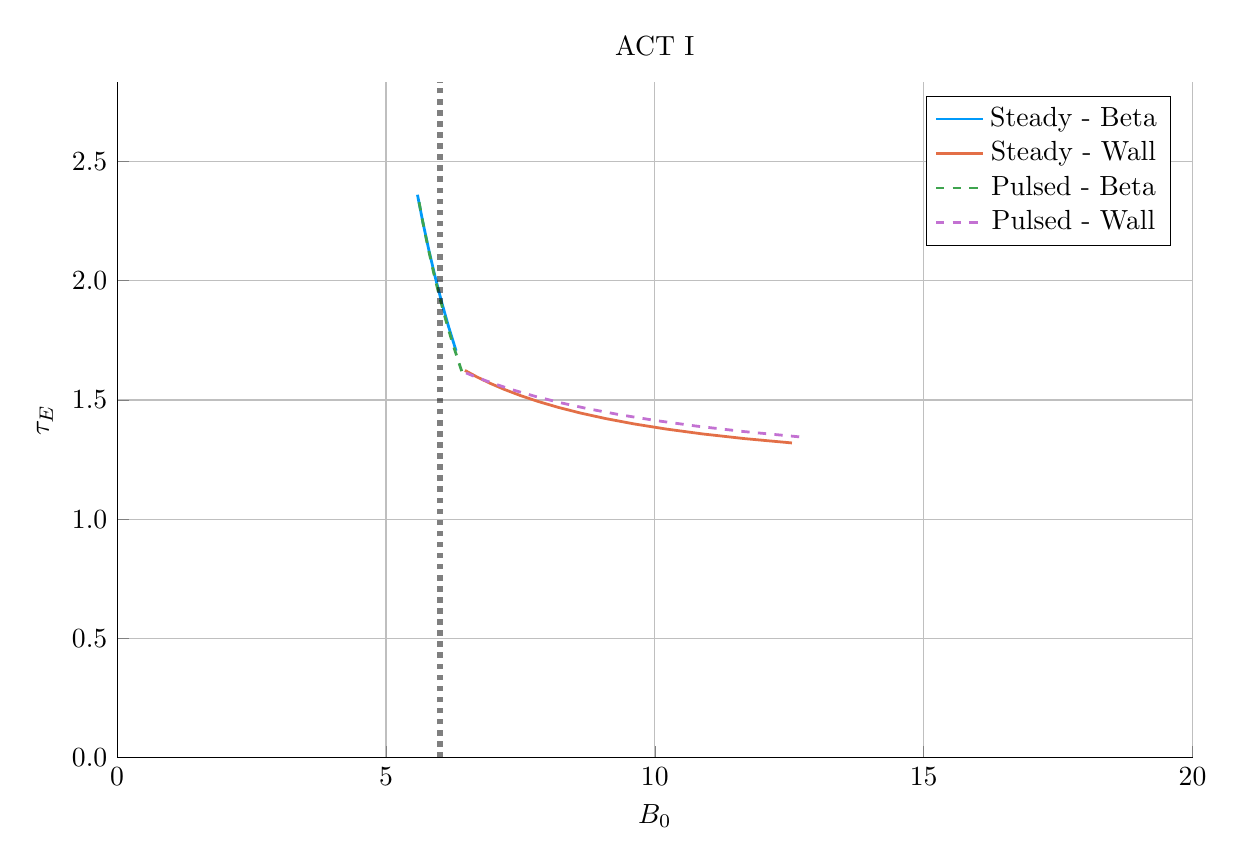
\begin{tikzpicture}[]
\begin{axis}[height = {101.6mm}, ylabel = {${\tau}_{E}$}, title = {ACT I}, xmin = {0.0}, xmax = {20.0}, ymax = {2.8326615360049403}, xlabel = {${B}_{0}$}, {unbounded coords=jump, scaled x ticks = false, xticklabel style={rotate = 0}, xmajorgrids = true, xtick = {0.0,5.0,10.0,15.0,20.0}, xticklabels = {0,5,10,15,20}, xtick align = inside, axis lines* = left, scaled y ticks = false, yticklabel style={rotate = 0}, ymajorgrids = true, ytick = {0.0,0.5,1.0,1.5,2.0,2.5}, yticklabels = {0.0,0.5,1.0,1.5,2.0,2.5}, ytick align = inside, axis lines* = left,     xshift = 0.0mm,
    yshift = 0.0mm,
    axis background/.style={fill={rgb,1:red,1.00000000;green,1.00000000;blue,1.00000000}}
, colorbar style={title=}}, ymin = {0.0}, width = {152.4mm}]\addplot+ [color = {rgb,1:red,0.00000000;green,0.60560316;blue,0.97868012},
draw opacity=1.0,
line width=1,
solid,mark = none,
mark size = 2.0,
mark options = {
    color = {rgb,1:red,0.00000000;green,0.00000000;blue,0.00000000}, draw opacity = 1.0,
    fill = {rgb,1:red,0.00000000;green,0.60560316;blue,0.97868012}, fill opacity = 1.0,
    line width = 1,
    rotate = 0,
    solid
}]coordinates {
(6.30336807958207, 1.7063788508721172)
(6.162193069273141, 1.8090537561194575)
(6.030717178404645, 1.9143387573902246)
(5.908065509576601, 2.0221834245249295)
(5.793464904530972, 2.132535952054342)
(5.686229631357383, 2.245343302905053)
(5.585749511271037, 2.360551280004117)
};
\addlegendentry{Steady - Beta}
\addplot+ [color = {rgb,1:red,0.88887350;green,0.43564919;blue,0.27812294},
draw opacity=1.0,
line width=1,
solid,mark = none,
mark size = 2.0,
mark options = {
    color = {rgb,1:red,0.00000000;green,0.00000000;blue,0.00000000}, draw opacity = 1.0,
    fill = {rgb,1:red,0.88887350;green,0.43564919;blue,0.27812294}, fill opacity = 1.0,
    line width = 1,
    rotate = 0,
    solid
}]coordinates {
(12.549536249695134, 1.319742732592967)
(11.658754653696462, 1.3381417436751073)
(10.883719833507003, 1.3576688166353064)
(10.206258129789394, 1.3782058500012966)
(9.611335769312953, 1.3996556420893593)
(9.086446934250878, 1.4219380885652215)
(8.62129895070743, 1.4449855548058383)
(8.207216040989662, 1.4687422433122175)
(7.837119555085499, 1.4931592651604135)
(7.505047858717157, 1.5181951378556127)
(7.20604322925957, 1.5438134897064264)
(6.935884710193303, 1.5699832015338886)
(6.691016583192173, 1.5966768574678945)
(6.468415485086983, 1.6238703579503406)
};
\addlegendentry{Steady - Wall}
\addplot+ [color = {rgb,1:red,0.24222430;green,0.64327509;blue,0.30444865},
draw opacity=1.0,
line width=1,
dashed,mark = none,
mark size = 2.0,
mark options = {
    color = {rgb,1:red,0.00000000;green,0.00000000;blue,0.00000000}, draw opacity = 1.0,
    fill = {rgb,1:red,0.24222430;green,0.64327509;blue,0.30444865}, fill opacity = 1.0,
    line width = 1,
    rotate = 0,
    solid
}]coordinates {
(6.408263337806559, 1.620988869607618)
(6.408263337806564, 1.620988869607615)
(6.385466513301022, 1.6359132395586664)
(6.245492502072912, 1.7329861734313399)
(6.116010320461132, 1.8320260474596086)
(5.9960421481916395, 1.9329445794038793)
(5.884727159112828, 2.035653552741772)
(5.781304768121868, 2.1400649788505506)
(5.685100648450046, 2.246091248334046)
(5.595515000321003, 2.353645273401782)
};
\addlegendentry{Pulsed - Beta}
\addplot+ [color = {rgb,1:red,0.76444018;green,0.44411178;blue,0.82429754},
draw opacity=1.0,
line width=1,
dashed,mark = none,
mark size = 2.0,
mark options = {
    color = {rgb,1:red,0.00000000;green,0.00000000;blue,0.00000000}, draw opacity = 1.0,
    fill = {rgb,1:red,0.76444018;green,0.44411178;blue,0.82429754}, fill opacity = 1.0,
    line width = 1,
    rotate = 0,
    solid
}]coordinates {
(12.684248532650473, 1.345389169271226)
(11.66307871570063, 1.3673467361979852)
(10.781888309639141, 1.3901603790598458)
(10.016282491385791, 1.4137627262589771)
(9.346943280276514, 1.438096070132187)
(8.758420158941194, 1.4631106777058556)
(8.238241792953433, 1.4887634440436004)
(7.776255600865612, 1.5150168096503511)
(7.364131118520045, 1.5418378835774142)
(6.994982564641668, 1.5691977280648413)
(6.66307916140573, 1.5970707712511294)
(6.408263337806559, 1.620988869607618)
(6.408263337806564, 1.620988869607615)
};
\addlegendentry{Pulsed - Wall}
\addplot+ [color = {rgb,1:red,0.00000000;green,0.00000000;blue,0.00000000},
draw opacity=0.5,
line width=2,
dotted,mark = none,
mark size = 2.0,
mark options = {
    color = {rgb,1:red,0.00000000;green,0.00000000;blue,0.00000000}, draw opacity = 0.5,
    fill = {rgb,1:red,0.00000000;green,0.00000000;blue,0.00000000}, fill opacity = 0.5,
    line width = 1,
    rotate = 0,
    solid
},forget plot]coordinates {
(0.0, NaN)
(20.0, NaN)
};
\addplot+ [color = {rgb,1:red,0.00000000;green,0.00000000;blue,0.00000000},
draw opacity=0.5,
line width=2,
dotted,mark = none,
mark size = 2.0,
mark options = {
    color = {rgb,1:red,0.00000000;green,0.00000000;blue,0.00000000}, draw opacity = 0.5,
    fill = {rgb,1:red,0.00000000;green,0.00000000;blue,0.00000000}, fill opacity = 0.5,
    line width = 1,
    rotate = 0,
    solid
},forget plot]coordinates {
(6.0, 0.0)
(6.0, 2.8326615360049403)
};
\addplot+[draw=none, color = {rgb,1:red,0.00000000;green,0.00000000;blue,0.00000000},
draw opacity=0.5,
line width=0,
solid,mark = *,
mark size = 2.0,
mark options = {
    color = {rgb,1:red,0.00000000;green,0.00000000;blue,0.00000000}, draw opacity = 0.5,
    fill = {rgb,1:red,0.00000000;green,0.00000000;blue,0.00000000}, fill opacity = 0.5,
    line width = 1,
    rotate = 0,
    solid
},forget plot] coordinates {
(6.0, NaN)
};
\end{axis}

\end{tikzpicture}

    \end{adjustbox}
        \caption{ACT I}
    \end{subfigure}
    \hfill
    \begin{subfigure}[t]{0.45\textwidth}
        \centering
    \begin{adjustbox}{width=\textwidth}
      \Large
      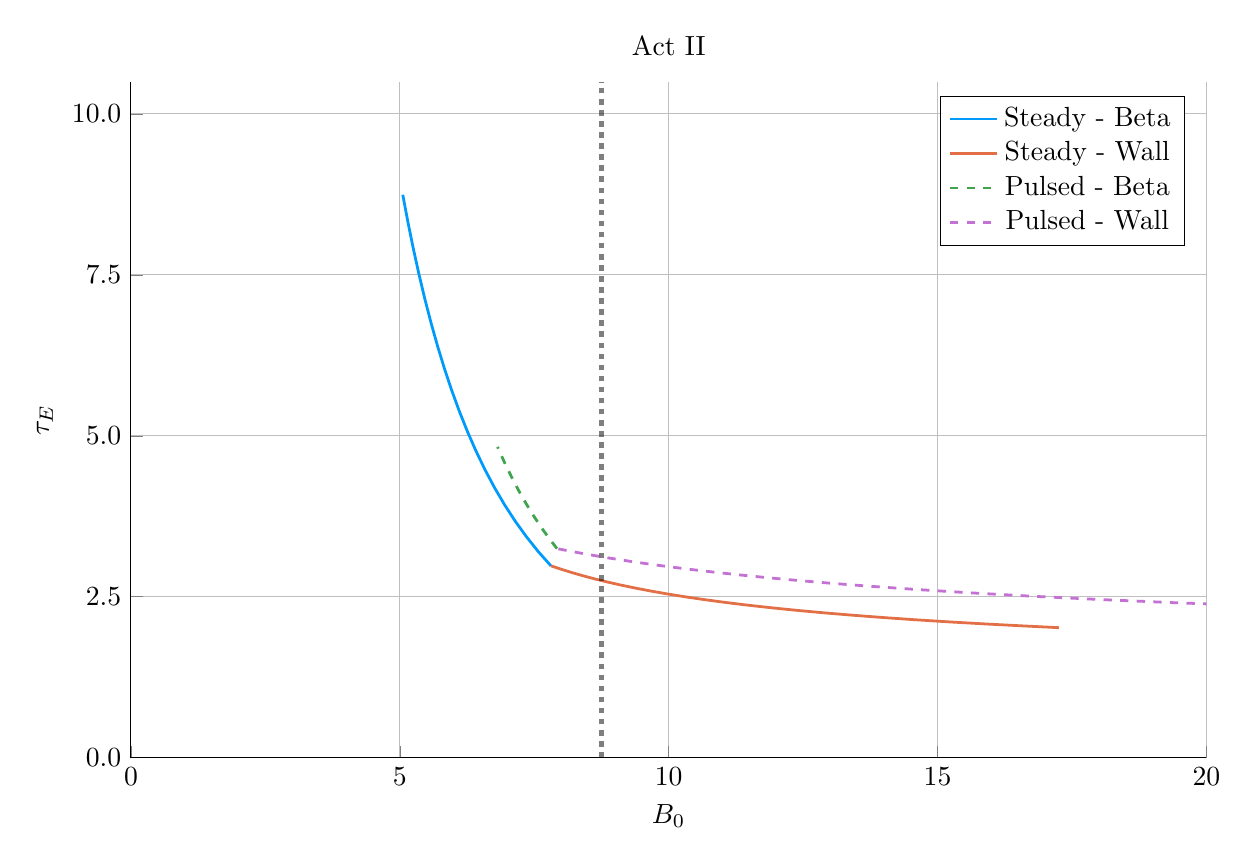
\begin{tikzpicture}[]
\begin{axis}[height = {101.6mm}, ylabel = {${\tau}_{E}$}, title = {Act II}, xmin = {0.0}, xmax = {20.0}, ymax = {10.492943910085124}, xlabel = {${B}_{0}$}, {unbounded coords=jump, scaled x ticks = false, xticklabel style={rotate = 0}, xmajorgrids = true, xtick = {0.0,5.0,10.0,15.0,20.0}, xticklabels = {0,5,10,15,20}, xtick align = inside, axis lines* = left, scaled y ticks = false, yticklabel style={rotate = 0}, ymajorgrids = true, ytick = {0.0,2.5,5.0,7.5,10.0}, yticklabels = {0.0,2.5,5.0,7.5,10.0}, ytick align = inside, axis lines* = left,     xshift = 0.0mm,
    yshift = 0.0mm,
    axis background/.style={fill={rgb,1:red,1.00000000;green,1.00000000;blue,1.00000000}}
, colorbar style={title=}}, ymin = {0.0}, width = {152.4mm}]\addplot+ [color = {rgb,1:red,0.00000000;green,0.60560316;blue,0.97868012},
draw opacity=1.0,
line width=1,
solid,mark = none,
mark size = 2.0,
mark options = {
    color = {rgb,1:red,0.00000000;green,0.00000000;blue,0.00000000}, draw opacity = 1.0,
    fill = {rgb,1:red,0.00000000;green,0.60560316;blue,0.97868012}, fill opacity = 1.0,
    line width = 1,
    rotate = 0,
    solid
}]coordinates {
(7.810935944285959, 2.9790315868503647)
(7.57736049850867, 3.198828217527613)
(7.354864292609041, 3.4312633131605925)
(7.145167234136329, 3.6747680732771757)
(6.9473303865083675, 3.9295223618791395)
(6.760499508614096, 4.195693690216852)
(6.583897990324067, 4.473434719288982)
(6.416817229618043, 4.7628841339936745)
(6.258609820663305, 5.064165989044067)
(6.108683264880386, 5.377389400038819)
(5.966494431410919, 5.702648280974925)
(5.831544666176381, 6.040021127085321)
(5.703375459679132, 6.389570848002029)
(5.581564609582325, 6.751344637344923)
(5.465722802994068, 7.12537389542732)
(5.355490573482678, 7.511674192515099)
(5.25053558682053, 7.91024526913508)
(5.1505502068221745, 8.321071089893742)
(5.0552493196883175, 8.744119925070937)
};
\addlegendentry{Steady - Beta}
\addplot+ [color = {rgb,1:red,0.88887350;green,0.43564919;blue,0.27812294},
draw opacity=1.0,
line width=1,
solid,mark = none,
mark size = 2.0,
mark options = {
    color = {rgb,1:red,0.00000000;green,0.00000000;blue,0.00000000}, draw opacity = 1.0,
    fill = {rgb,1:red,0.88887350;green,0.43564919;blue,0.27812294}, fill opacity = 1.0,
    line width = 1,
    rotate = 0,
    solid
}]coordinates {
(17.25550839059296, 2.0191079061319352)
(16.594334962335296, 2.0464338960635517)
(15.9071755430688, 2.076210182141703)
(15.233983138507648, 2.1079936106627897)
(14.594239858921854, 2.14147850222047)
(13.989673082630297, 2.1765055734908776)
(13.414782495717416, 2.212997910097208)
(12.872659546281994, 2.250814948778079)
(12.364365715508608, 2.2898406747224653)
(11.889507953196574, 2.329980135836693)
(11.44685939646348, 2.3711544570152476)
(11.034739998180656, 2.4132973404359728)
(10.651252523287319, 2.456352514678312)
(10.294428800132035, 2.5002718216139987)
(9.962319203963213, 2.54501374948921)
(9.653045819449929, 2.590542287904863)
(9.364832254395445, 2.6368260209964967)
(9.096018465506306, 2.683837400397078)
(8.844373144802077, 2.7315647198098523)
(8.61055754360846, 2.7799488152935936)
(8.391192178573277, 2.829008304413284)
(8.18577947665566, 2.878713620421055)
(7.99323348423048, 2.929049519766908)
(7.812301489248497, 2.980008177415489)
};
\addlegendentry{Steady - Wall}
\addplot+ [color = {rgb,1:red,0.24222430;green,0.64327509;blue,0.30444865},
draw opacity=1.0,
line width=1,
dashed,mark = none,
mark size = 2.0,
mark options = {
    color = {rgb,1:red,0.00000000;green,0.00000000;blue,0.00000000}, draw opacity = 1.0,
    fill = {rgb,1:red,0.24222430;green,0.64327509;blue,0.30444865}, fill opacity = 1.0,
    line width = 1,
    rotate = 0,
    solid
}]coordinates {
(7.923668284887995, 3.24748621603794)
(7.923668284887995, 3.2474862160379465)
(7.836759696043437, 3.340092370097236)
(7.6662731560983355, 3.5341535488145444)
(7.50499428233835, 3.73445223905736)
(7.35232773269976, 3.94093479607719)
(7.207727224738343, 4.153536285091506)
(7.070690693175276, 4.372180683576633)
(6.940756001029682, 4.596781123613878)
(6.817497143644154, 4.82724016130744)
};
\addlegendentry{Pulsed - Beta}
\addplot+ [color = {rgb,1:red,0.76444018;green,0.44411178;blue,0.82429754},
draw opacity=1.0,
line width=1,
dashed,mark = none,
mark size = 2.0,
mark options = {
    color = {rgb,1:red,0.00000000;green,0.00000000;blue,0.00000000}, draw opacity = 1.0,
    fill = {rgb,1:red,0.76444018;green,0.44411178;blue,0.82429754}, fill opacity = 1.0,
    line width = 1,
    rotate = 0,
    solid
}]coordinates {
(22.56106430311702, 2.313954958641652)
(20.85607192394036, 2.361244949920411)
(19.335265246056654, 2.409367818812461)
(17.974121547130903, 2.4582968513042665)
(16.751976718553127, 2.508007846778854)
(15.651329744019142, 2.558478785582883)
(14.65728744097675, 2.6096895509351876)
(13.757118584462601, 2.6616216930573584)
(12.939893642194303, 2.714258228189006)
(12.196191964860315, 2.76758346666229)
(11.517862472405039, 2.8215828653003063)
(10.897827027335556, 2.8762429002384944)
(10.329918077124672, 2.9315509571104443)
(9.808743940706389, 2.9874952356288498)
(9.329576544487265, 3.0440646668017957)
(8.888257451278507, 3.10124884063848)
(8.481118883411932, 3.1590379429401287)
(8.10491708701527, 3.217422699871154)
(7.923668284887995, 3.24748621603794)
(7.923668284887995, 3.2474862160379465)
};
\addlegendentry{Pulsed - Wall}
\addplot+ [color = {rgb,1:red,0.00000000;green,0.00000000;blue,0.00000000},
draw opacity=0.5,
line width=2,
dotted,mark = none,
mark size = 2.0,
mark options = {
    color = {rgb,1:red,0.00000000;green,0.00000000;blue,0.00000000}, draw opacity = 0.5,
    fill = {rgb,1:red,0.00000000;green,0.00000000;blue,0.00000000}, fill opacity = 0.5,
    line width = 1,
    rotate = 0,
    solid
},forget plot]coordinates {
(0.0, NaN)
(20.0, NaN)
};
\addplot+ [color = {rgb,1:red,0.00000000;green,0.00000000;blue,0.00000000},
draw opacity=0.5,
line width=2,
dotted,mark = none,
mark size = 2.0,
mark options = {
    color = {rgb,1:red,0.00000000;green,0.00000000;blue,0.00000000}, draw opacity = 0.5,
    fill = {rgb,1:red,0.00000000;green,0.00000000;blue,0.00000000}, fill opacity = 0.5,
    line width = 1,
    rotate = 0,
    solid
},forget plot]coordinates {
(8.75, 0.0)
(8.75, 10.492943910085124)
};
\addplot+[draw=none, color = {rgb,1:red,0.00000000;green,0.00000000;blue,0.00000000},
draw opacity=0.5,
line width=0,
solid,mark = *,
mark size = 2.0,
mark options = {
    color = {rgb,1:red,0.00000000;green,0.00000000;blue,0.00000000}, draw opacity = 0.5,
    fill = {rgb,1:red,0.00000000;green,0.00000000;blue,0.00000000}, fill opacity = 0.5,
    line width = 1,
    rotate = 0,
    solid
},forget plot] coordinates {
(8.75, NaN)
};
\end{axis}

\end{tikzpicture}

    \end{adjustbox}
        \caption{ACT II}
    \end{subfigure}
    \hfill \hfill ~\\ ~\\ ~\\ ~\\
  \caption[]{Magnet Scan: $\tau_E$ vs $B_0$} ~\\
\end{figure*}


\clearpage

\newpage

\subsection*{ Current Drive Efficiency -- $\eta_{CD}$ }
  \label{subsection:scan_eta_CD}

\begin{figure*}[h!]
    \centering
    \hfill
    \begin{subfigure}[t]{0.45\textwidth}
        \centering
    \begin{adjustbox}{width=\textwidth}
      \Large
      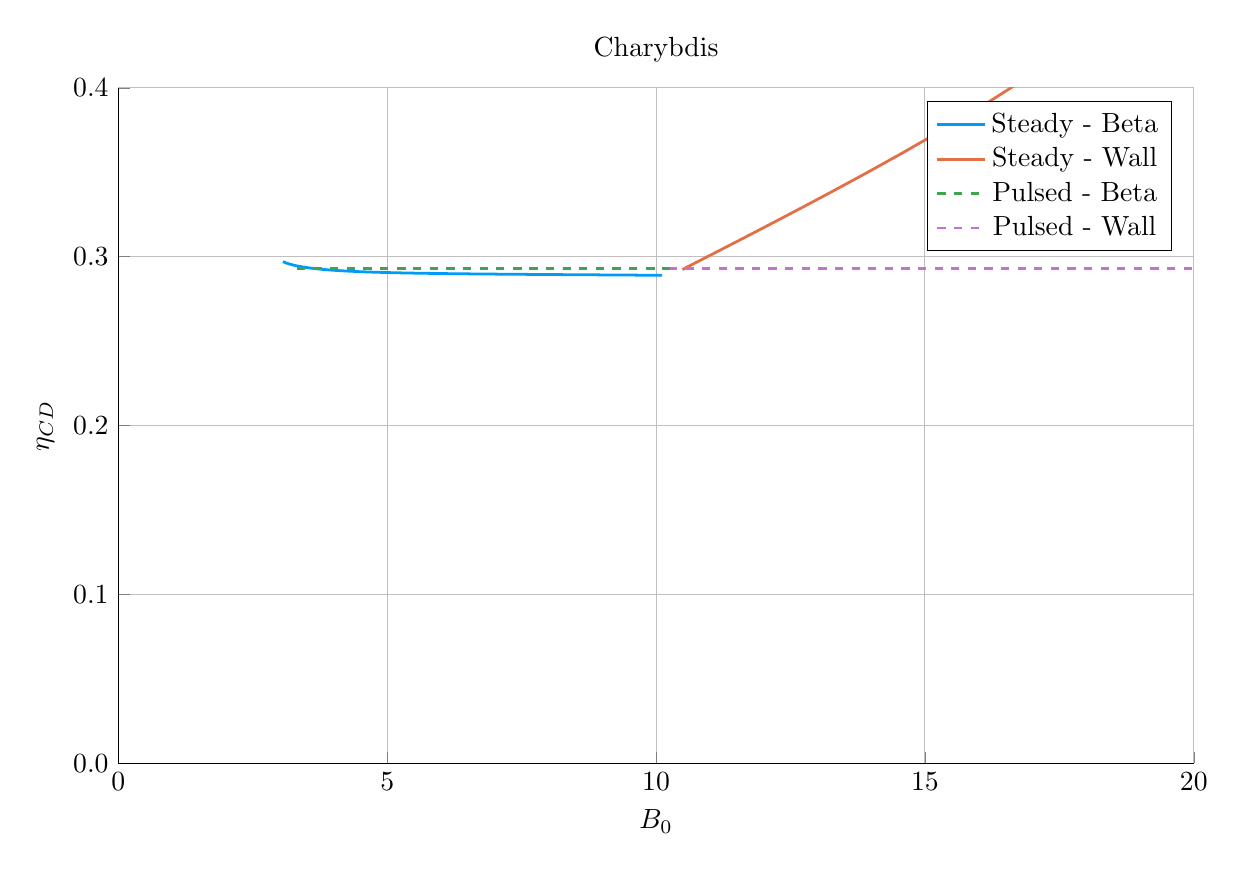
\begin{tikzpicture}[]
\begin{axis}[height = {101.6mm}, ylabel = {${\eta}_{CD}$}, title = {Charybdis}, xmin = {0.0}, xmax = {20.0}, ymax = {0.4}, xlabel = {${B}_{0}$}, {unbounded coords=jump, scaled x ticks = false, xticklabel style={rotate = 0}, xmajorgrids = true, xtick = {0.0,5.0,10.0,15.0,20.0}, xticklabels = {0,5,10,15,20}, xtick align = inside, axis lines* = left, scaled y ticks = false, yticklabel style={rotate = 0}, ymajorgrids = true, ytick = {0.0,0.1,0.2,0.30000000000000004,0.4}, yticklabels = {0.0,0.1,0.2,0.3,0.4}, ytick align = inside, axis lines* = left,     xshift = 0.0mm,
    yshift = 0.0mm,
    axis background/.style={fill={rgb,1:red,1.00000000;green,1.00000000;blue,1.00000000}}
, colorbar style={title=}}, ymin = {0.0}, width = {152.4mm}]\addplot+ [color = {rgb,1:red,0.00000000;green,0.60560316;blue,0.97868012},
draw opacity=1.0,
line width=1,
solid,mark = none,
mark size = 2.0,
mark options = {
    color = {rgb,1:red,0.00000000;green,0.00000000;blue,0.00000000}, draw opacity = 1.0,
    fill = {rgb,1:red,0.00000000;green,0.60560316;blue,0.97868012}, fill opacity = 1.0,
    line width = 1,
    rotate = 0,
    solid
}]coordinates {
(10.112818033153026, 0.2890124001708679)
(9.722156888543116, 0.2890934058074779)
(9.357875603858393, 0.28916957864023385)
(9.017653755630063, 0.289241971718532)
(8.6995124437054, 0.2893093526110478)
(8.401566530516865, 0.28937346296062694)
(8.122163706328223, 0.2894349713924345)
(7.859819415455661, 0.28949448265460487)
(7.613196557650265, 0.28955254309932243)
(7.381088038653343, 0.2896096457184144)
(7.162401716104116, 0.28966623476343445)
(6.956147367527331, 0.2897227099799709)
(6.761425371986388, 0.28977943048511107)
(6.577416849463348, 0.28983671831577723)
(6.403375044688587, 0.28989486167423906)
(6.2386177769852695, 0.2899541178955051)
(6.0825208065966905, 0.2900147161612859)
(5.934511989185341, 0.2900768599723193)
(5.794066116682695, 0.29014072942323216)
(5.660700347012839, 0.29020648326562526)
(5.533970150598111, 0.2902742608008287)
(5.413465705416883, 0.2903441836068744)
(5.298808685607224, 0.2904163571218577)
(5.189649392059402, 0.29049087208037166)
(5.085664187259174, 0.2905678058370994)
(4.986553195072601, 0.29064722357133665)
(4.892038235455667, 0.29072917938928644)
(4.801860966679364, 0.29081371733194217)
(4.7157812114040425, 0.2909008722967884)
(4.633575445956479, 0.2909906708807873)
(4.5550354347559185, 0.29108313215149306)
(4.479966994069385, 0.29117826835249444)
(4.408188871204256, 0.29127608554886664)
(4.33953172691477, 0.2913765842177861)
(4.273837210246432, 0.2914797597890203)
(4.210957116299974, 0.2915856031395779)
(4.15075261849161, 0.2916941010464348)
(4.0930935678432965, 0.2918052366009017)
(4.037857852672517, 0.29191898958788354)
(3.9849308127842145, 0.29203533683300315)
(3.9342047029103653, 0.29215425252029686)
(3.8855782007091695, 0.2922757084829535)
(3.838955955133626, 0.2923996744693585)
(3.7942481714200484, 0.29252611838650283)
(3.7513702293348077, 0.29265500652264587)
(3.710242331663442, 0.29278630375095266)
(3.6707891802306123, 0.2929199737156832)
(3.6329396770109583, 0.2930559790023756)
(3.5966266481325166, 0.2931942812933425)
(3.5617865887889004, 0.2933348415096877)
(3.5283594272686503, 0.29347761994094823)
(3.496288306480746, 0.2936225763633821)
(3.465519381509793, 0.2937696701478163)
(3.4360016318699595, 0.2939188603579226)
(3.4076866872513096, 0.29407010583968624)
(3.380528665662031, 0.2942233653027989)
(3.3544840229690007, 0.2943785973946173)
(3.3295114129297314, 0.29453576076730204)
(3.3055715568879336, 0.2946948141386861)
(3.2826271223788512, 0.2948557163473816)
(3.260642607548369, 0.29501842638145964)
(3.239584247604666, 0.29518290352905774)
(3.2194198921826622, 0.29534910720753893)
(3.2001189373344725, 0.29551699721118)
(3.181652227422265, 0.2956865336381098)
(3.163991977015565, 0.2958576769405733)
(3.1471116955378684, 0.29603038795087755)
(3.130986116696265, 0.2962046279044162)
(3.115591132350856, 0.2963803584600108)
(3.1009037305081053, 0.29655754171778737)
(3.0869019371473265, 0.2967361402347924)
(3.0735647616124355, 0.2969161170385373)
(3.0608721453218655, 0.2970974356386405)
};
\addlegendentry{Steady - Beta}
\addplot+ [color = {rgb,1:red,0.88887350;green,0.43564919;blue,0.27812294},
draw opacity=1.0,
line width=1,
solid,mark = none,
mark size = 2.0,
mark options = {
    color = {rgb,1:red,0.00000000;green,0.00000000;blue,0.00000000}, draw opacity = 1.0,
    fill = {rgb,1:red,0.88887350;green,0.43564919;blue,0.27812294}, fill opacity = 1.0,
    line width = 1,
    rotate = 0,
    solid
}]coordinates {
(20.758867641064707, 0.550619788361201)
(20.346250098246923, 0.5079685190808274)
(19.57104597888471, 0.47503902985770124)
(18.681781921115476, 0.44813959090357636)
(17.775790175980152, 0.4255015286239918)
(16.896654716492492, 0.406077367741247)
(16.063927450323227, 0.3891772930411093)
(15.285557510665852, 0.3743136422319958)
(14.563500533069154, 0.36112607873138414)
(13.896568848875791, 0.349339912602884)
(13.281970890030232, 0.33874072709065145)
(12.716170469467318, 0.32915795214509086)
(12.195372283741088, 0.32045374568641577)
(11.715794270833433, 0.3125152089271154)
(11.273815669498969, 0.3052487883586615)
(10.866051794088186, 0.29857616101982265)
(10.489365023931143, 0.2924314183330621)
};
\addlegendentry{Steady - Wall}
\addplot+ [color = {rgb,1:red,0.24222430;green,0.64327509;blue,0.30444865},
draw opacity=1.0,
line width=1,
dashed,mark = none,
mark size = 2.0,
mark options = {
    color = {rgb,1:red,0.00000000;green,0.00000000;blue,0.00000000}, draw opacity = 1.0,
    fill = {rgb,1:red,0.24222430;green,0.64327509;blue,0.30444865}, fill opacity = 1.0,
    line width = 1,
    rotate = 0,
    solid
}]coordinates {
(10.26788634689966, 0.29282)
(9.953967652326213, 0.29282)
(9.567926244368271, 0.29282)
(9.207974394987358, 0.29282)
(8.871841888699304, 0.29282)
(8.557505525932248, 0.29282)
(8.263156925406376, 0.29282)
(7.9871752024348766, 0.29282)
(7.728103682045175, 0.29282)
(7.484629973620137, 0.29282)
(7.255568856523303, 0.29282)
(7.039847526735421, 0.29282)
(6.836492834698909, 0.29282)
(6.644620209081183, 0.29282)
(6.463424013335149, 0.29282)
(6.2921691243175495, 0.29282)
(6.13018355681404, 0.29282)
(5.97685198655569, 0.29282)
(5.831610044919842, 0.29282)
(5.693939286027163, 0.29282)
(5.563362729090489, 0.29282)
(5.439440906144732, 0.29282)
(5.321768347746793, 0.29282)
(5.209970453003084, 0.29282)
(5.103700692769835, 0.29282)
(5.002638109938164, 0.29282)
(4.906485077678376, 0.29282)
(4.814965286571576, 0.29282)
(4.727821933804548, 0.29282)
(4.644816091323922, 0.29282)
(4.565725232806084, 0.29282)
(4.490341901840154, 0.29282)
(4.418472505906755, 0.29282)
(4.349936222622964, 0.29282)
(4.284564006352339, 0.29282)
(4.222197684694192, 0.29282)
(4.162689135592264, 0.29282)
(4.105899536872315, 0.29282)
(4.051698680949713, 0.29282)
(3.9999643482627323, 0.29282)
(3.9505817337017928, 0.29282)
(3.903442920928527, 0.29282)
(3.858446400032002, 0.29282)
(3.8154966244515616, 0.29282)
(3.7745036035252744, 0.29282)
(3.7353825273991994, 0.29282)
(3.6980534213689746, 0.29282)
(3.6624408270205375, 0.29282)
(3.62847350780097, 0.29282)
(3.5960841768845415, 0.29282)
(3.565209245407392, 0.29282)
(3.5357885893311605, 0.29282)
(3.5077653333614305, 0.29282)
(3.4810856504959875, 0.29282)
(3.4556985759109375, 0.29282)
(3.4315558340122845, 0.29282)
(3.408611677587535, 0.29282)
(3.3868227380888998, 0.29282)
(3.36614788616562, 0.29282)
(3.3465481016421226, 0.29282)
(3.327986352208224, 0.29282)
(3.3104274769652595, 0.29282)
(3.2938380965241474, 0.29282)
(3.278186482171801, 0.29282)
(3.263442495132517, 0.29282)
(3.2495774839156075, 0.29282)
(3.236564206241785, 0.29282)
(3.224376752844934, 0.29282)
(3.212990475972638, 0.29282)
(3.2023819222517877, 0.29282)
(3.192528769611062, 0.29282)
(3.1834097679780142, 0.29282)
(3.1750046834890777, 0.29282)
(3.1672942459724482, 0.29282)
};
\addlegendentry{Pulsed - Beta}
\addplot+ [color = {rgb,1:red,0.76444018;green,0.44411178;blue,0.82429754},
draw opacity=1.0,
line width=1,
dashed,mark = none,
mark size = 2.0,
mark options = {
    color = {rgb,1:red,0.00000000;green,0.00000000;blue,0.00000000}, draw opacity = 1.0,
    fill = {rgb,1:red,0.76444018;green,0.44411178;blue,0.82429754}, fill opacity = 1.0,
    line width = 1,
    rotate = 0,
    solid
}]coordinates {
(48.990476413653056, 0.29282)
(42.83950920694117, 0.29282)
(37.687790427214495, 0.29282)
(33.33937742845888, 0.29282)
(29.64296398154308, 0.29282)
(26.48039367255613, 0.29282)
(23.758442882319894, 0.29282)
(21.402860298405816, 0.29282)
(19.353987387634486, 0.29282)
(17.563502020363714, 0.29282)
(15.991970371213752, 0.29282)
(14.606987499719377, 0.29282)
(13.381751501116137, 0.29282)
(12.293960329570087, 0.29282)
(11.32495111804522, 0.29282)
(10.459023415380802, 0.29282)
(10.26788634689966, 0.29282)
};
\addlegendentry{Pulsed - Wall}
\end{axis}

\end{tikzpicture}

    \end{adjustbox}
        \caption{Charybdis}
    \end{subfigure}
    \hfill
    \begin{subfigure}[t]{0.45\textwidth}
        \centering
    \begin{adjustbox}{width=\textwidth}
      \Large
      \begin{tikzpicture}[]
\begin{axis}[height = {101.6mm}, ylabel = {${\eta}_{CD}$}, title = {Proteus}, xmin = {0.0}, xmax = {20.0}, ymax = {0.75}, xlabel = {${B}_{0}$}, {unbounded coords=jump, scaled x ticks = false, xticklabel style={rotate = 0}, xmajorgrids = true, xtick = {0.0,5.0,10.0,15.0,20.0}, xticklabels = {0,5,10,15,20}, xtick align = inside, axis lines* = left, scaled y ticks = false, yticklabel style={rotate = 0}, ymajorgrids = true, ytick = {0.0,0.25,0.5,0.75}, yticklabels = {0.00,0.25,0.50,0.75}, ytick align = inside, axis lines* = left,     xshift = 0.0mm,
    yshift = 0.0mm,
    axis background/.style={fill={rgb,1:red,1.00000000;green,1.00000000;blue,1.00000000}}
, colorbar style={title=}}, ymin = {0.0}, width = {152.4mm}]\addplot+ [color = {rgb,1:red,0.00000000;green,0.60560316;blue,0.97868012},
draw opacity=1.0,
line width=1,
solid,mark = none,
mark size = 2.0,
mark options = {
    color = {rgb,1:red,0.00000000;green,0.00000000;blue,0.00000000}, draw opacity = 1.0,
    fill = {rgb,1:red,0.00000000;green,0.60560316;blue,0.97868012}, fill opacity = 1.0,
    line width = 1,
    rotate = 0,
    solid
}]coordinates {
(4.658732060637907, 0.0)
(4.211109766361548, 0.0)
(3.9293920326356777, 0.0)
(3.7651903683456465, 0.0)
(3.6776039543745567, 0.0)
(3.6402437753208394, 0.0)
(3.6366994671255806, 0.0)
(3.656621534643579, 0.0)
(3.693300156736026, 0.0)
(3.7422515017241134, 0.0)
(3.865532743079537, 0.0)
(3.936096932264377, 0.0)
(4.010907188015084, 0.0)
(4.089072356933184, 0.0)
(4.169903401491354, 0.0)
(4.252857906625248, 0.0)
(4.337501757261618, 0.0)
(4.42348218754058, 0.0)
(4.5983381267510195, 0.0)
(4.686766232902671, 0.0)
(4.775618142770625, 0.0)
(4.864743502376605, 0.0)
(4.927312314219091, 0.0)
};
\addlegendentry{Pulsed - Kink}
\addplot+ [color = {rgb,1:red,0.88887350;green,0.43564919;blue,0.27812294},
draw opacity=1.0,
line width=1,
solid,mark = none,
mark size = 2.0,
mark options = {
    color = {rgb,1:red,0.00000000;green,0.00000000;blue,0.00000000}, draw opacity = 1.0,
    fill = {rgb,1:red,0.88887350;green,0.43564919;blue,0.27812294}, fill opacity = 1.0,
    line width = 1,
    rotate = 0,
    solid
}]coordinates {
(4.927312314219091, 0.0)
(4.984545814413324, 0.0)
(5.17452482724068, 0.0)
(5.362091669637646, 0.0)
(5.54700293215903, 0.0)
(5.729042482638278, 0.0)
(5.908022832274664, 0.0)
(6.083785777786694, 0.0)
(6.256202341425288, 0.0)
(6.324169421042356, 0.0)
};
\addlegendentry{Pulsed - Beta}
\addplot+ [color = {rgb,1:red,0.24222430;green,0.64327509;blue,0.30444865},
draw opacity=1.0,
line width=1,
solid,mark = none,
mark size = 2.0,
mark options = {
    color = {rgb,1:red,0.00000000;green,0.00000000;blue,0.00000000}, draw opacity = 1.0,
    fill = {rgb,1:red,0.24222430;green,0.64327509;blue,0.30444865}, fill opacity = 1.0,
    line width = 1,
    rotate = 0,
    solid
}]coordinates {
(6.324169421042356, 0.0)
(6.727338549778396, 0.0)
(7.320469048424473, 0.0)
(7.835746509376305, 0.0)
(8.290245520072391, 0.0)
(8.696162676727877, 0.0)
(9.0624397222742, 0.0)
(9.395798186463841, 0.0)
(9.701405747258567, 0.0)
(10.244760202900984, 0.0)
(10.930275827723788, 0.0)
(11.131878682735255, 0.0)
(11.50278450645086, 0.0)
(11.83715172742864, 0.0)
(11.992609772603878, 0.0)
(12.141110720831467, 0.0)
};
\addlegendentry{Pulsed - Wall}
\end{axis}

\end{tikzpicture}

    \end{adjustbox}
        \caption{Proteus}
    \end{subfigure}
    \hfill \hfill ~\\ ~\\ ~\\ ~\\
    \hfill
    \begin{subfigure}[t]{0.45\textwidth}
        \centering
    \begin{adjustbox}{width=\textwidth}
      \Large
      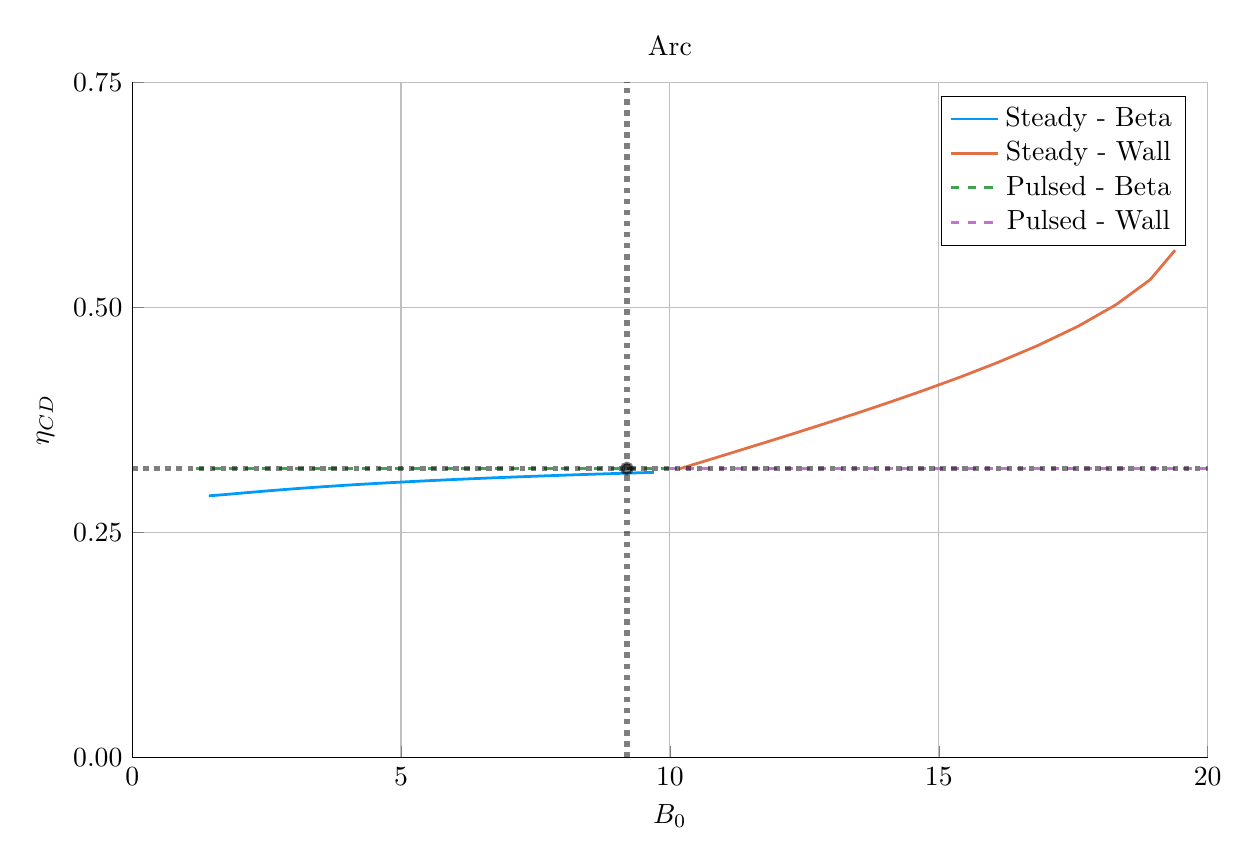
\begin{tikzpicture}[]
\begin{axis}[height = {101.6mm}, ylabel = {${\eta}_{CD}$}, title = {Arc}, xmin = {0.0}, xmax = {20.0}, ymax = {0.75}, xlabel = {${B}_{0}$}, {unbounded coords=jump, scaled x ticks = false, xticklabel style={rotate = 0}, xmajorgrids = true, xtick = {0.0,5.0,10.0,15.0,20.0}, xticklabels = {0,5,10,15,20}, xtick align = inside, axis lines* = left, scaled y ticks = false, yticklabel style={rotate = 0}, ymajorgrids = true, ytick = {0.0,0.25,0.5,0.75}, yticklabels = {0.00,0.25,0.50,0.75}, ytick align = inside, axis lines* = left,     xshift = 0.0mm,
    yshift = 0.0mm,
    axis background/.style={fill={rgb,1:red,1.00000000;green,1.00000000;blue,1.00000000}}
, colorbar style={title=}}, ymin = {0.0}, width = {152.4mm}]\addplot+ [color = {rgb,1:red,0.00000000;green,0.60560316;blue,0.97868012},
draw opacity=1.0,
line width=1,
solid,mark = none,
mark size = 2.0,
mark options = {
    color = {rgb,1:red,0.00000000;green,0.00000000;blue,0.00000000}, draw opacity = 1.0,
    fill = {rgb,1:red,0.00000000;green,0.60560316;blue,0.97868012}, fill opacity = 1.0,
    line width = 1,
    rotate = 0,
    solid
}]coordinates {
(9.701206080853105, 0.31678518115648574)
(9.162315904693079, 0.31583089394216074)
(8.664301107137337, 0.3149011884023737)
(8.203576462497304, 0.31399350083262684)
(7.776718537485166, 0.3131085665987562)
(7.380720231870917, 0.312246226189249)
(7.012886014999712, 0.3114062859136451)
(6.670795005901889, 0.3105885224708399)
(6.352268997292712, 0.30979268706272084)
(6.055344682097163, 0.3090185090895425)
(5.778249464564785, 0.308265699462471)
(5.519380338856715, 0.30753395356715885)
(5.2772854007125325, 0.3068229539102666)
(5.050647625972996, 0.3061323724787059)
(4.838270606140816, 0.3054618728391684)
(4.639065978019038, 0.3048111120033003)
(4.4520423235376105, 0.3041797420817258)
(4.276295348572609, 0.3035674117480987)
(4.110999177018484, 0.302973767532411)
(3.9553986195015125, 0.3023984549610117)
(3.8088022956698633, 0.30184111955911525)
(3.6705765055641186, 0.30130140773005787)
(3.54013975965751, 0.30077896752416283)
(3.4169578891619192, 0.3002734493087987)
(3.30053966845824, 0.29978450635006315)
(3.1904328903033052, 0.2993117953154708)
(3.086220842019516, 0.2988549767060812)
(2.9875191373772063, 0.29841371522564203)
(2.8939728644914635, 0.29798768009355203)
(2.8052540149097247, 0.2975765453077553)
(2.7210591632720242, 0.2971799898630477)
(2.6411073705789065, 0.29679769792971905)
(2.565138287279709, 0.29642935899694256)
(2.492910435164382, 0.29607466798487375)
(2.4241996494611984, 0.29573332532900987)
(2.3587976646588236, 0.2954050370399923)
(2.296510829425685, 0.29508951474171063)
(2.237158937627476, 0.2947864756902631)
(2.180574163874242, 0.29449564277607226)
(2.126600093288366, 0.2942167445112054)
(2.075090836295778, 0.29394951500374616)
(2.0259102202234582, 0.2936936939208607)
(1.978931050353818, 0.2934490264420379)
(1.9340344338545452, 0.29321526320382335)
(1.8911091606836798, 0.2929921602372276)
(1.8500511361739687, 0.2927794788988655)
(1.8107628605384507, 0.29257698579677005)
(1.773152951016952, 0.29238445271172375)
(1.7371357028100902, 0.29220165651485824)
(1.7026306853269466, 0.29202837908219315)
(1.6695623706125668, 0.2918644072067112)
(1.6378597911249178, 0.29170953250849796)
(1.607456224302725, 0.29156355134342243)
(1.5782889016090462, 0.29142626471077193)
(1.5502987399539199, 0.2912974781602151)
(1.5234300935954943, 0.29117700169841804)
(1.4976305247952577, 0.29106464969560597)
(1.4728505916614916, 0.29096024079231986)
(1.4490436517578602, 0.29086359780659643)
(1.4261656801829077, 0.29077454764176025)
};
\addlegendentry{Steady - Beta}
\addplot+ [color = {rgb,1:red,0.88887350;green,0.43564919;blue,0.27812294},
draw opacity=1.0,
line width=1,
solid,mark = none,
mark size = 2.0,
mark options = {
    color = {rgb,1:red,0.00000000;green,0.00000000;blue,0.00000000}, draw opacity = 1.0,
    fill = {rgb,1:red,0.88887350;green,0.43564919;blue,0.27812294}, fill opacity = 1.0,
    line width = 1,
    rotate = 0,
    solid
}]coordinates {
(19.394007482712425, 0.5634549799653227)
(18.932196567189358, 0.5307387645778467)
(18.296989378345195, 0.502932838538793)
(17.587029315408756, 0.4788538284858783)
(16.847882407994106, 0.45777559766527154)
(16.111374502564406, 0.43913697422784204)
(15.396027314547156, 0.4225189070778569)
(14.710952688793137, 0.4076075232878504)
(14.06168447794857, 0.39414824695195777)
(13.450465418483889, 0.3819378378662276)
(12.877644538645335, 0.370810567048703)
(12.342394470642008, 0.36062970930202726)
(11.843182246608265, 0.35128131489391323)
(11.376441269625893, 0.34268105839610163)
(10.944966372727551, 0.3347131725686331)
(10.541663878705513, 0.32734277008606677)
(10.165908182236457, 0.320499462119806)
};
\addlegendentry{Steady - Wall}
\addplot+ [color = {rgb,1:red,0.24222430;green,0.64327509;blue,0.30444865},
draw opacity=1.0,
line width=1,
dashed,mark = none,
mark size = 2.0,
mark options = {
    color = {rgb,1:red,0.00000000;green,0.00000000;blue,0.00000000}, draw opacity = 1.0,
    fill = {rgb,1:red,0.24222430;green,0.64327509;blue,0.30444865}, fill opacity = 1.0,
    line width = 1,
    rotate = 0,
    solid
}]coordinates {
(9.980483622051658, 0.321)
(9.392786903460065, 0.321)
(8.79273598103983, 0.321)
(8.23820290909994, 0.321)
(7.725182218401588, 0.321)
(7.250078106370205, 0.321)
(6.80965553466646, 0.321)
(6.400998063035608, 0.321)
(6.0214713600430425, 0.321)
(5.668691517461799, 0.321)
(5.340497445229901, 0.321)
(5.034926745580058, 0.321)
(4.750194564008521, 0.321)
(4.484674995755211, 0.321)
(4.236884692979903, 0.321)
(4.00546837264544, 0.321)
(3.7891859704718387, 0.321)
(3.5869012239550364, 0.321)
(3.3975714987448393, 0.321)
(3.2202386987489797, 0.321)
(3.0540211220494466, 0.321)
(2.8981061427709687, 0.321)
(2.7517436139566023, 0.321)
(2.6142398986781377, 0.321)
(2.4849524463010138, 0.321)
(2.363284838174807, 0.321)
(2.248682232019848, 0.321)
(2.140627136740878, 0.321)
(2.038635448877246, 0.321)
(1.9422526775794744, 0.321)
(1.8510502754751532, 0.321)
(1.7646219756564088, 0.321)
(1.6825800061969869, 0.321)
(1.6045510059627948, 0.321)
(1.53017138625397, 0.321)
(1.4590817483192686, 0.321)
(1.3909197311384796, 0.321)
(1.3253102336217724, 0.321)
(1.261851128383913, 0.321)
(1.20009089049112, 0.321)
(1.1394908096975784, 0.321)
};
\addlegendentry{Pulsed - Beta}
\addplot+ [color = {rgb,1:red,0.76444018;green,0.44411178;blue,0.82429754},
draw opacity=1.0,
line width=1,
dashed,mark = none,
mark size = 2.0,
mark options = {
    color = {rgb,1:red,0.00000000;green,0.00000000;blue,0.00000000}, draw opacity = 1.0,
    fill = {rgb,1:red,0.76444018;green,0.44411178;blue,0.82429754}, fill opacity = 1.0,
    line width = 1,
    rotate = 0,
    solid
}]coordinates {
(29.27715761652869, 0.321)
(25.4410619834368, 0.321)
(22.158819835998365, 0.321)
(19.342453256965573, 0.321)
(16.919364280634177, 0.321)
(14.829378672669455, 0.321)
(13.022412368922526, 0.321)
(11.456617692058645, 0.321)
(10.096901921254785, 0.321)
(9.980483622051658, 0.321)
};
\addlegendentry{Pulsed - Wall}
\addplot+ [color = {rgb,1:red,0.00000000;green,0.00000000;blue,0.00000000},
draw opacity=0.5,
line width=2,
dotted,mark = none,
mark size = 2.0,
mark options = {
    color = {rgb,1:red,0.00000000;green,0.00000000;blue,0.00000000}, draw opacity = 0.5,
    fill = {rgb,1:red,0.00000000;green,0.00000000;blue,0.00000000}, fill opacity = 0.5,
    line width = 1,
    rotate = 0,
    solid
},forget plot]coordinates {
(0.0, 0.321)
(20.0, 0.321)
};
\addplot+ [color = {rgb,1:red,0.00000000;green,0.00000000;blue,0.00000000},
draw opacity=0.5,
line width=2,
dotted,mark = none,
mark size = 2.0,
mark options = {
    color = {rgb,1:red,0.00000000;green,0.00000000;blue,0.00000000}, draw opacity = 0.5,
    fill = {rgb,1:red,0.00000000;green,0.00000000;blue,0.00000000}, fill opacity = 0.5,
    line width = 1,
    rotate = 0,
    solid
},forget plot]coordinates {
(9.2, 0.0)
(9.2, 0.75)
};
\addplot+[draw=none, color = {rgb,1:red,0.00000000;green,0.00000000;blue,0.00000000},
draw opacity=0.5,
line width=0,
solid,mark = *,
mark size = 2.0,
mark options = {
    color = {rgb,1:red,0.00000000;green,0.00000000;blue,0.00000000}, draw opacity = 0.5,
    fill = {rgb,1:red,0.00000000;green,0.00000000;blue,0.00000000}, fill opacity = 0.5,
    line width = 1,
    rotate = 0,
    solid
},forget plot] coordinates {
(9.2, 0.321)
};
\end{axis}

\end{tikzpicture}

    \end{adjustbox}
        \caption{ARC}
    \end{subfigure}
    \hfill
    \begin{subfigure}[t]{0.45\textwidth}
        \centering
    \begin{adjustbox}{width=\textwidth}
      \Large
      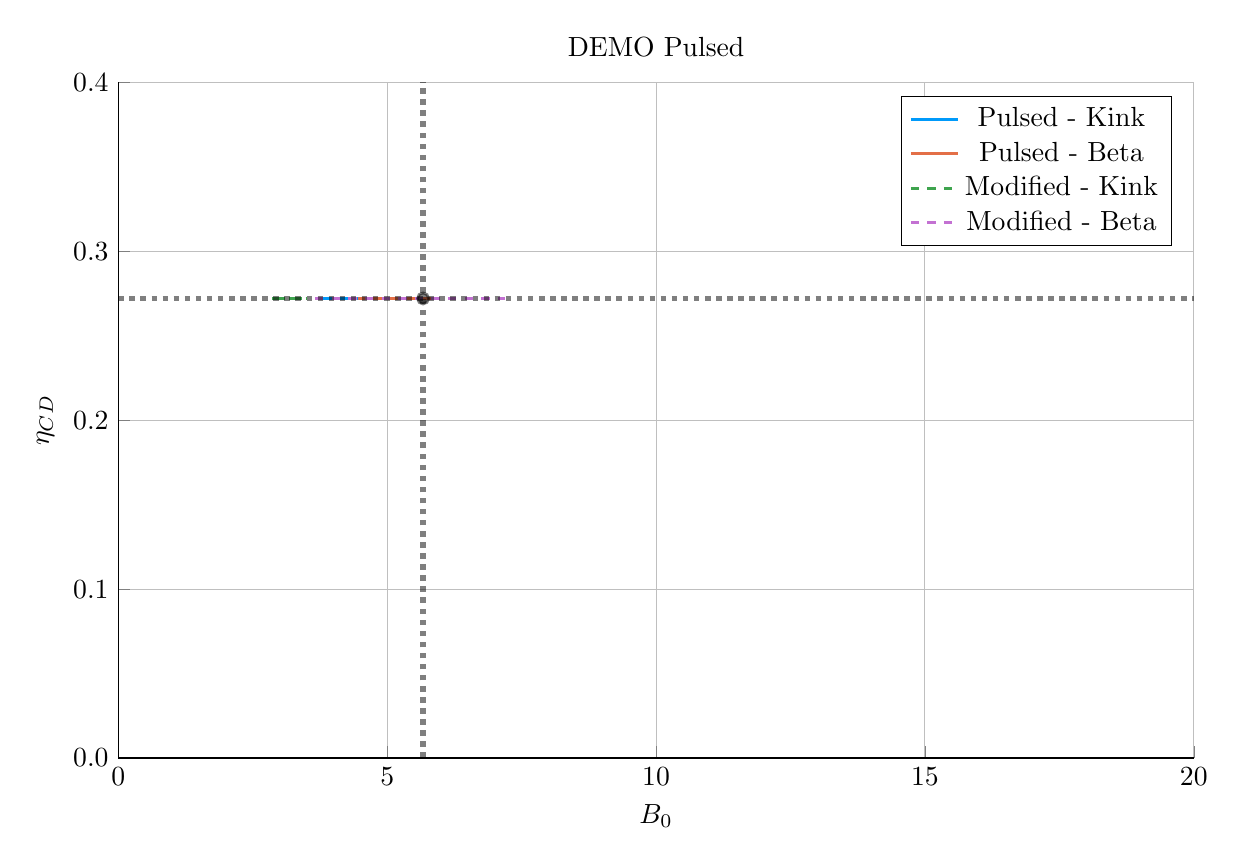
\begin{tikzpicture}[]
\begin{axis}[height = {101.6mm}, ylabel = {${\eta}_{CD}$}, title = {DEMO Pulsed}, xmin = {0.0}, xmax = {20.0}, ymax = {0.4}, xlabel = {${B}_{0}$}, {unbounded coords=jump, scaled x ticks = false, xticklabel style={rotate = 0}, xmajorgrids = true, xtick = {0.0,5.0,10.0,15.0,20.0}, xticklabels = {0,5,10,15,20}, xtick align = inside, axis lines* = left, scaled y ticks = false, yticklabel style={rotate = 0}, ymajorgrids = true, ytick = {0.0,0.1,0.2,0.30000000000000004,0.4}, yticklabels = {0.0,0.1,0.2,0.3,0.4}, ytick align = inside, axis lines* = left,     xshift = 0.0mm,
    yshift = 0.0mm,
    axis background/.style={fill={rgb,1:red,1.00000000;green,1.00000000;blue,1.00000000}}
, colorbar style={title=}}, ymin = {0.0}, width = {152.4mm}]\addplot+ [color = {rgb,1:red,0.00000000;green,0.60560316;blue,0.97868012},
draw opacity=1.0,
line width=1,
solid,mark = none,
mark size = 2.0,
mark options = {
    color = {rgb,1:red,0.00000000;green,0.00000000;blue,0.00000000}, draw opacity = 1.0,
    fill = {rgb,1:red,0.00000000;green,0.60560316;blue,0.97868012}, fill opacity = 1.0,
    line width = 1,
    rotate = 0,
    solid
}]coordinates {
(4.327031075670194, 0.2721)
(4.038214026054326, 0.2721)
(3.8713719163129245, 0.2721)
(3.7758613845615545, 0.2721)
(3.7257856761317214, 0.2721)
(3.7090473695925437, 0.2721)
(3.727711597554826, 0.2721)
(3.7586131667481433, 0.2721)
(3.799052518631718, 0.2721)
(3.901290136389271, 0.2721)
(3.960577465316514, 0.2721)
(4.0241209645210345, 0.2721)
(4.0912717805663785, 0.2721)
(4.161514602943343, 0.2721)
(4.2344343960723005, 0.2721)
(4.309692554546368, 0.2721)
(4.450417240491067, 0.2721)
};
\addlegendentry{Pulsed - Kink}
\addplot+ [color = {rgb,1:red,0.88887350;green,0.43564919;blue,0.27812294},
draw opacity=1.0,
line width=1,
solid,mark = none,
mark size = 2.0,
mark options = {
    color = {rgb,1:red,0.00000000;green,0.00000000;blue,0.00000000}, draw opacity = 1.0,
    fill = {rgb,1:red,0.88887350;green,0.43564919;blue,0.27812294}, fill opacity = 1.0,
    line width = 1,
    rotate = 0,
    solid
}]coordinates {
(4.450417240491067, 0.2721)
(4.490148631384312, 0.2721)
(4.692490181445514, 0.2721)
(4.8960344619053355, 0.2721)
(5.100651132702229, 0.2721)
(5.306202822090688, 0.2721)
(5.512545696627038, 0.2721)
(5.719530043226767, 0.2721)
(5.927000883375481, 0.2721)
};
\addlegendentry{Pulsed - Beta}
\addplot+ [color = {rgb,1:red,0.24222430;green,0.64327509;blue,0.30444865},
draw opacity=1.0,
line width=1,
dashed,mark = none,
mark size = 2.0,
mark options = {
    color = {rgb,1:red,0.00000000;green,0.00000000;blue,0.00000000}, draw opacity = 1.0,
    fill = {rgb,1:red,0.24222430;green,0.64327509;blue,0.30444865}, fill opacity = 1.0,
    line width = 1,
    rotate = 0,
    solid
}]coordinates {
(3.4087424183072135, 0.2721)
(2.977074181068944, 0.2721)
(2.8592500074202523, 0.2721)
(2.827199220063259, 0.2721)
(2.8339789008667826, 0.2721)
(2.862412302880871, 0.2721)
(2.9044598258085443, 0.2721)
(2.95577893007882, 0.2721)
(3.0137895352525907, 0.2721)
(3.076849710218805, 0.2721)
(3.1438583711612704, 0.2721)
(3.214045733980633, 0.2721)
(3.2868548955983727, 0.2721)
(3.361871149981842, 0.2721)
(3.4387778750377818, 0.2721)
(3.5173279629378453, 0.2721)
};
\addlegendentry{Modified - Kink}
\addplot+ [color = {rgb,1:red,0.76444018;green,0.44411178;blue,0.82429754},
draw opacity=1.0,
line width=1,
dashed,mark = none,
mark size = 2.0,
mark options = {
    color = {rgb,1:red,0.00000000;green,0.00000000;blue,0.00000000}, draw opacity = 1.0,
    fill = {rgb,1:red,0.76444018;green,0.44411178;blue,0.82429754}, fill opacity = 1.0,
    line width = 1,
    rotate = 0,
    solid
}]coordinates {
(3.6607028750648505, 0.2721)
(3.8574448036470477, 0.2721)
(4.056375867871351, 0.2721)
(4.257366397480293, 0.2721)
(4.460279103534801, 0.2721)
(4.664969389370631, 0.2721)
(4.871285596007394, 0.2721)
(5.07906923307514, 0.2721)
(5.288155233306219, 0.2721)
(5.498372259673351, 0.2721)
(5.709543087166185, 0.2721)
(5.921485076209294, 0.2721)
(6.134010749367255, 0.2721)
(6.346928478632384, 0.2721)
(6.560043285872518, 0.2721)
(6.773157754368795, 0.2721)
(6.986073044284746, 0.2721)
(7.198590001107076, 0.2721)
};
\addlegendentry{Modified - Beta}
\addplot+ [color = {rgb,1:red,0.00000000;green,0.00000000;blue,0.00000000},
draw opacity=0.5,
line width=2,
dotted,mark = none,
mark size = 2.0,
mark options = {
    color = {rgb,1:red,0.00000000;green,0.00000000;blue,0.00000000}, draw opacity = 0.5,
    fill = {rgb,1:red,0.00000000;green,0.00000000;blue,0.00000000}, fill opacity = 0.5,
    line width = 1,
    rotate = 0,
    solid
},forget plot]coordinates {
(0.0, 0.2721)
(20.0, 0.2721)
};
\addplot+ [color = {rgb,1:red,0.00000000;green,0.00000000;blue,0.00000000},
draw opacity=0.5,
line width=2,
dotted,mark = none,
mark size = 2.0,
mark options = {
    color = {rgb,1:red,0.00000000;green,0.00000000;blue,0.00000000}, draw opacity = 0.5,
    fill = {rgb,1:red,0.00000000;green,0.00000000;blue,0.00000000}, fill opacity = 0.5,
    line width = 1,
    rotate = 0,
    solid
},forget plot]coordinates {
(5.667, 0.0)
(5.667, 0.4)
};
\addplot+[draw=none, color = {rgb,1:red,0.00000000;green,0.00000000;blue,0.00000000},
draw opacity=0.5,
line width=0,
solid,mark = *,
mark size = 2.0,
mark options = {
    color = {rgb,1:red,0.00000000;green,0.00000000;blue,0.00000000}, draw opacity = 0.5,
    fill = {rgb,1:red,0.00000000;green,0.00000000;blue,0.00000000}, fill opacity = 0.5,
    line width = 1,
    rotate = 0,
    solid
},forget plot] coordinates {
(5.667, 0.2721)
};
\end{axis}

\end{tikzpicture}

    \end{adjustbox}
        \caption{DEMO Pulsed}
    \end{subfigure}
    \hfill \hfill ~\\ ~\\ ~\\ ~\\
    \hfill
    \begin{subfigure}[t]{0.45\textwidth}
        \centering
    \begin{adjustbox}{width=\textwidth}
      \Large
      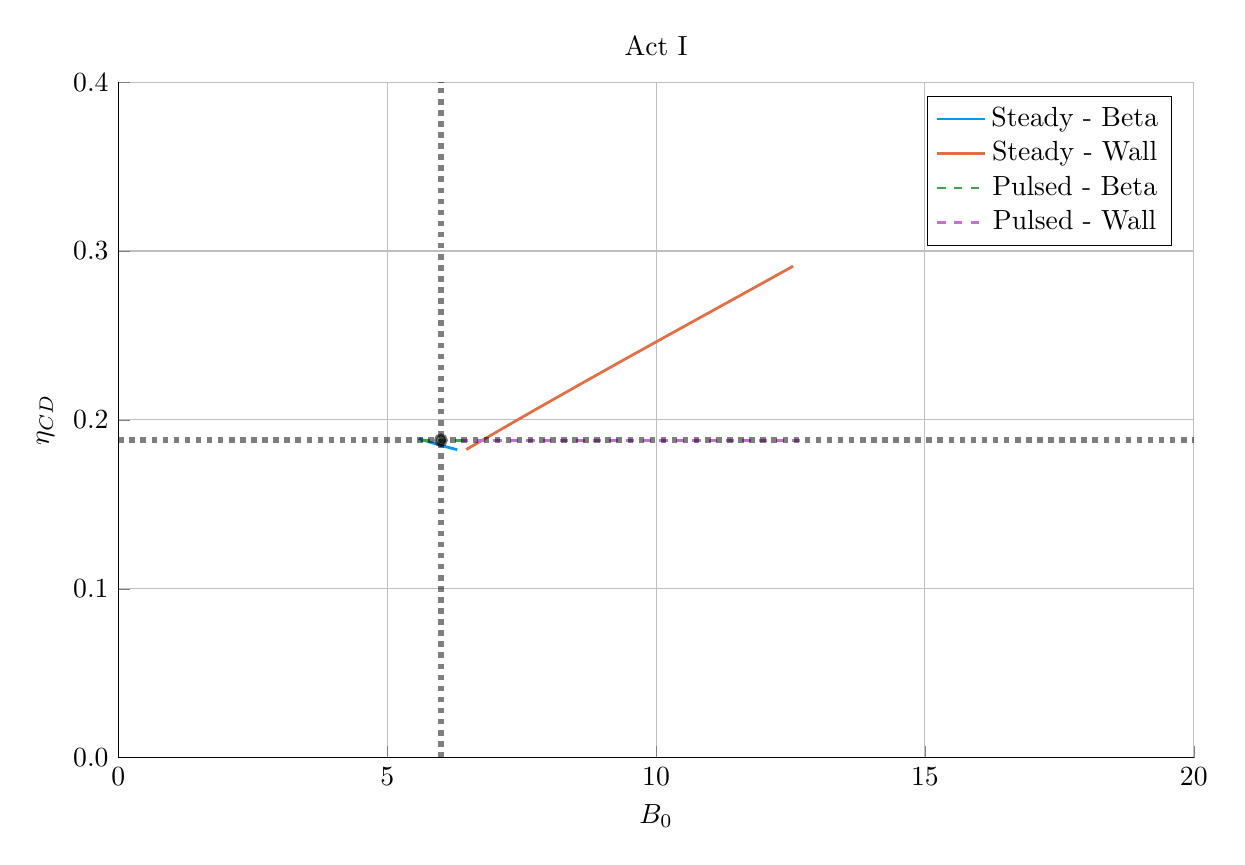
\begin{tikzpicture}[]
\begin{axis}[height = {101.6mm}, ylabel = {${\eta}_{CD}$}, title = {Act I}, xmin = {0.0}, xmax = {20.0}, ymax = {0.4}, xlabel = {${B}_{0}$}, {unbounded coords=jump, scaled x ticks = false, xticklabel style={rotate = 0}, xmajorgrids = true, xtick = {0.0,5.0,10.0,15.0,20.0}, xticklabels = {0,5,10,15,20}, xtick align = inside, axis lines* = left, scaled y ticks = false, yticklabel style={rotate = 0}, ymajorgrids = true, ytick = {0.0,0.1,0.2,0.30000000000000004,0.4}, yticklabels = {0.0,0.1,0.2,0.3,0.4}, ytick align = inside, axis lines* = left,     xshift = 0.0mm,
    yshift = 0.0mm,
    axis background/.style={fill={rgb,1:red,1.00000000;green,1.00000000;blue,1.00000000}}
, colorbar style={title=}}, ymin = {0.0}, width = {152.4mm}]\addplot+ [color = {rgb,1:red,0.00000000;green,0.60560316;blue,0.97868012},
draw opacity=1.0,
line width=1,
solid,mark = none,
mark size = 2.0,
mark options = {
    color = {rgb,1:red,0.00000000;green,0.00000000;blue,0.00000000}, draw opacity = 1.0,
    fill = {rgb,1:red,0.00000000;green,0.60560316;blue,0.97868012}, fill opacity = 1.0,
    line width = 1,
    rotate = 0,
    solid
}]coordinates {
(6.30336807958207, 0.1823561352356704)
(6.162193069273141, 0.1835100392239879)
(6.030717178404645, 0.18464133914026942)
(5.908065509576601, 0.18575084586057625)
(5.793464904530972, 0.18683932522483726)
(5.686229631357383, 0.18790751323540555)
(5.585749511271037, 0.18895611587938982)
};
\addlegendentry{Steady - Beta}
\addplot+ [color = {rgb,1:red,0.88887350;green,0.43564919;blue,0.27812294},
draw opacity=1.0,
line width=1,
solid,mark = none,
mark size = 2.0,
mark options = {
    color = {rgb,1:red,0.00000000;green,0.00000000;blue,0.00000000}, draw opacity = 1.0,
    fill = {rgb,1:red,0.88887350;green,0.43564919;blue,0.27812294}, fill opacity = 1.0,
    line width = 1,
    rotate = 0,
    solid
}]coordinates {
(12.549536249695134, 0.2910608626327861)
(11.658754653696462, 0.27535234723802104)
(10.883719833507003, 0.2617365572638159)
(10.206258129789394, 0.24982583018256505)
(9.611335769312953, 0.23932460746277257)
(9.086446934250878, 0.23000733607526727)
(8.62129895070743, 0.2216938630555514)
(8.207216040989662, 0.21424667065579228)
(7.837119555085499, 0.20754757687479983)
(7.505047858717157, 0.20150165571841783)
(7.20604322925957, 0.196027716416671)
(6.935884710193303, 0.19105965902449665)
(6.691016583192173, 0.1865405392519257)
(6.468415485086983, 0.1824216502403495)
};
\addlegendentry{Steady - Wall}
\addplot+ [color = {rgb,1:red,0.24222430;green,0.64327509;blue,0.30444865},
draw opacity=1.0,
line width=1,
dashed,mark = none,
mark size = 2.0,
mark options = {
    color = {rgb,1:red,0.00000000;green,0.00000000;blue,0.00000000}, draw opacity = 1.0,
    fill = {rgb,1:red,0.24222430;green,0.64327509;blue,0.30444865}, fill opacity = 1.0,
    line width = 1,
    rotate = 0,
    solid
}]coordinates {
(6.408263337806559, 0.188)
(6.408263337806564, 0.188)
(6.385466513301022, 0.188)
(6.245492502072912, 0.188)
(6.116010320461132, 0.188)
(5.9960421481916395, 0.188)
(5.884727159112828, 0.188)
(5.781304768121868, 0.188)
(5.685100648450046, 0.188)
(5.595515000321003, 0.188)
};
\addlegendentry{Pulsed - Beta}
\addplot+ [color = {rgb,1:red,0.76444018;green,0.44411178;blue,0.82429754},
draw opacity=1.0,
line width=1,
dashed,mark = none,
mark size = 2.0,
mark options = {
    color = {rgb,1:red,0.00000000;green,0.00000000;blue,0.00000000}, draw opacity = 1.0,
    fill = {rgb,1:red,0.76444018;green,0.44411178;blue,0.82429754}, fill opacity = 1.0,
    line width = 1,
    rotate = 0,
    solid
}]coordinates {
(12.684248532650473, 0.188)
(11.66307871570063, 0.188)
(10.781888309639141, 0.188)
(10.016282491385791, 0.188)
(9.346943280276514, 0.188)
(8.758420158941194, 0.188)
(8.238241792953433, 0.188)
(7.776255600865612, 0.188)
(7.364131118520045, 0.188)
(6.994982564641668, 0.188)
(6.66307916140573, 0.188)
(6.408263337806559, 0.188)
(6.408263337806564, 0.188)
};
\addlegendentry{Pulsed - Wall}
\addplot+ [color = {rgb,1:red,0.00000000;green,0.00000000;blue,0.00000000},
draw opacity=0.5,
line width=2,
dotted,mark = none,
mark size = 2.0,
mark options = {
    color = {rgb,1:red,0.00000000;green,0.00000000;blue,0.00000000}, draw opacity = 0.5,
    fill = {rgb,1:red,0.00000000;green,0.00000000;blue,0.00000000}, fill opacity = 0.5,
    line width = 1,
    rotate = 0,
    solid
},forget plot]coordinates {
(0.0, 0.188)
(20.0, 0.188)
};
\addplot+ [color = {rgb,1:red,0.00000000;green,0.00000000;blue,0.00000000},
draw opacity=0.5,
line width=2,
dotted,mark = none,
mark size = 2.0,
mark options = {
    color = {rgb,1:red,0.00000000;green,0.00000000;blue,0.00000000}, draw opacity = 0.5,
    fill = {rgb,1:red,0.00000000;green,0.00000000;blue,0.00000000}, fill opacity = 0.5,
    line width = 1,
    rotate = 0,
    solid
},forget plot]coordinates {
(6.0, 0.0)
(6.0, 0.4)
};
\addplot+[draw=none, color = {rgb,1:red,0.00000000;green,0.00000000;blue,0.00000000},
draw opacity=0.5,
line width=0,
solid,mark = *,
mark size = 2.0,
mark options = {
    color = {rgb,1:red,0.00000000;green,0.00000000;blue,0.00000000}, draw opacity = 0.5,
    fill = {rgb,1:red,0.00000000;green,0.00000000;blue,0.00000000}, fill opacity = 0.5,
    line width = 1,
    rotate = 0,
    solid
},forget plot] coordinates {
(6.0, 0.188)
};
\end{axis}

\end{tikzpicture}

    \end{adjustbox}
        \caption{ACT I}
    \end{subfigure}
    \hfill
    \begin{subfigure}[t]{0.45\textwidth}
        \centering
    \begin{adjustbox}{width=\textwidth}
      \Large
      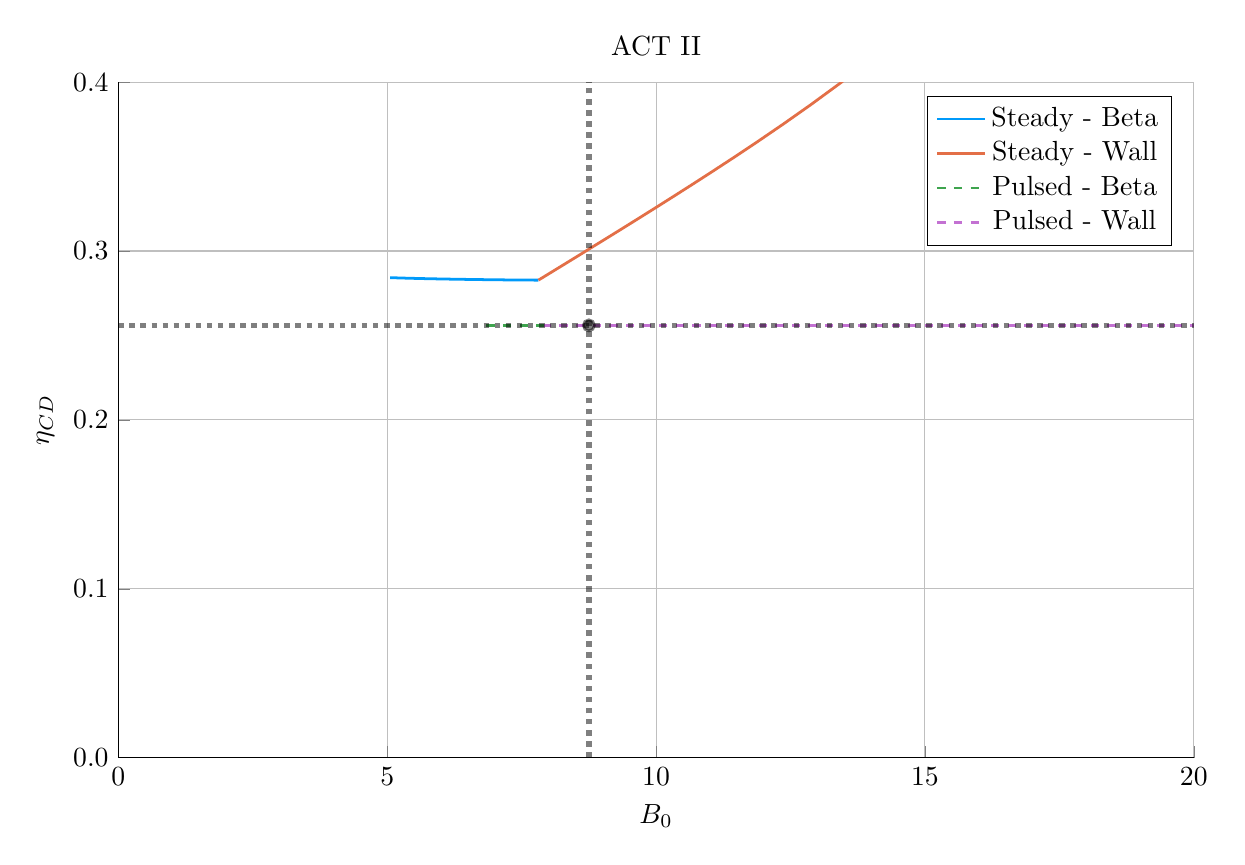
\begin{tikzpicture}[]
\begin{axis}[height = {101.6mm}, ylabel = {${\eta}_{CD}$}, title = {ACT II}, xmin = {0.0}, xmax = {20.0}, ymax = {0.4}, xlabel = {${B}_{0}$}, {unbounded coords=jump, scaled x ticks = false, xticklabel style={rotate = 0}, xmajorgrids = true, xtick = {0.0,5.0,10.0,15.0,20.0}, xticklabels = {0,5,10,15,20}, xtick align = inside, axis lines* = left, scaled y ticks = false, yticklabel style={rotate = 0}, ymajorgrids = true, ytick = {0.0,0.1,0.2,0.30000000000000004,0.4}, yticklabels = {0.0,0.1,0.2,0.3,0.4}, ytick align = inside, axis lines* = left,     xshift = 0.0mm,
    yshift = 0.0mm,
    axis background/.style={fill={rgb,1:red,1.00000000;green,1.00000000;blue,1.00000000}}
, colorbar style={title=}}, ymin = {0.0}, width = {152.4mm}]\addplot+ [color = {rgb,1:red,0.00000000;green,0.60560316;blue,0.97868012},
draw opacity=1.0,
line width=1,
solid,mark = none,
mark size = 2.0,
mark options = {
    color = {rgb,1:red,0.00000000;green,0.00000000;blue,0.00000000}, draw opacity = 1.0,
    fill = {rgb,1:red,0.00000000;green,0.60560316;blue,0.97868012}, fill opacity = 1.0,
    line width = 1,
    rotate = 0,
    solid
}]coordinates {
(7.810935944285959, 0.28278385416666674)
(7.57736049850867, 0.2827941507289973)
(7.354864292609041, 0.2828656869521074)
(7.145167234136329, 0.28293815875959166)
(6.9473303865083675, 0.2830117965664356)
(6.760499508614096, 0.2830868321928946)
(6.583897990324067, 0.2831634492975429)
(6.416817229618043, 0.28324181802286813)
(6.258609820663305, 0.2833220889583183)
(6.108683264880386, 0.28340439476492124)
(5.966494431410919, 0.2834888516761452)
(5.831544666176381, 0.2835755608862115)
(5.703375459679132, 0.28366460981555924)
(5.581564609582325, 0.2837560733063697)
(5.465722802994068, 0.28385001469534027)
(5.355490573482678, 0.2839464868119591)
(5.25053558682053, 0.2840455329111322)
(5.1505502068221745, 0.2841471874988046)
(5.0552493196883175, 0.28425147712316096)
};
\addlegendentry{Steady - Beta}
\addplot+ [color = {rgb,1:red,0.88887350;green,0.43564919;blue,0.27812294},
draw opacity=1.0,
line width=1,
solid,mark = none,
mark size = 2.0,
mark options = {
    color = {rgb,1:red,0.00000000;green,0.00000000;blue,0.00000000}, draw opacity = 1.0,
    fill = {rgb,1:red,0.88887350;green,0.43564919;blue,0.27812294}, fill opacity = 1.0,
    line width = 1,
    rotate = 0,
    solid
}]coordinates {
(17.25550839059296, 0.5164283784311735)
(16.594334962335296, 0.4898264674989419)
(15.9071755430688, 0.46692073063071027)
(15.233983138507648, 0.4468729633343918)
(14.594239858921854, 0.429110728237219)
(13.989673082630297, 0.4132921762874863)
(13.414782495717416, 0.399196773362045)
(12.872659546281994, 0.38655780777936233)
(12.364365715508608, 0.37516094244872894)
(11.889507953196574, 0.36483372494514577)
(11.44685939646348, 0.3554353741300471)
(11.034739998180656, 0.3468495700179973)
(10.651252523287319, 0.338979205266383)
(10.294428800132035, 0.3317424739147248)
(9.962319203963213, 0.32506990173948963)
(9.653045819449929, 0.3189020565125925)
(9.364832254395445, 0.3131877592521041)
(9.096018465506306, 0.3078826708262386)
(8.844373144802077, 0.3029561686837293)
(8.61055754360846, 0.2983504136707035)
(8.391192178573277, 0.2940596608531839)
(8.18577947665566, 0.29004960653622697)
(7.99323348423048, 0.28629689545530235)
(7.812301489248497, 0.2827838541666666)
};
\addlegendentry{Steady - Wall}
\addplot+ [color = {rgb,1:red,0.24222430;green,0.64327509;blue,0.30444865},
draw opacity=1.0,
line width=1,
dashed,mark = none,
mark size = 2.0,
mark options = {
    color = {rgb,1:red,0.00000000;green,0.00000000;blue,0.00000000}, draw opacity = 1.0,
    fill = {rgb,1:red,0.24222430;green,0.64327509;blue,0.30444865}, fill opacity = 1.0,
    line width = 1,
    rotate = 0,
    solid
}]coordinates {
(7.923668284887995, 0.256)
(7.923668284887995, 0.256)
(7.836759696043437, 0.256)
(7.6662731560983355, 0.256)
(7.50499428233835, 0.256)
(7.35232773269976, 0.256)
(7.207727224738343, 0.256)
(7.070690693175276, 0.256)
(6.940756001029682, 0.256)
(6.817497143644154, 0.256)
};
\addlegendentry{Pulsed - Beta}
\addplot+ [color = {rgb,1:red,0.76444018;green,0.44411178;blue,0.82429754},
draw opacity=1.0,
line width=1,
dashed,mark = none,
mark size = 2.0,
mark options = {
    color = {rgb,1:red,0.00000000;green,0.00000000;blue,0.00000000}, draw opacity = 1.0,
    fill = {rgb,1:red,0.76444018;green,0.44411178;blue,0.82429754}, fill opacity = 1.0,
    line width = 1,
    rotate = 0,
    solid
}]coordinates {
(22.56106430311702, 0.256)
(20.85607192394036, 0.256)
(19.335265246056654, 0.256)
(17.974121547130903, 0.256)
(16.751976718553127, 0.256)
(15.651329744019142, 0.256)
(14.65728744097675, 0.256)
(13.757118584462601, 0.256)
(12.939893642194303, 0.256)
(12.196191964860315, 0.256)
(11.517862472405039, 0.256)
(10.897827027335556, 0.256)
(10.329918077124672, 0.256)
(9.808743940706389, 0.256)
(9.329576544487265, 0.256)
(8.888257451278507, 0.256)
(8.481118883411932, 0.256)
(8.10491708701527, 0.256)
(7.923668284887995, 0.256)
(7.923668284887995, 0.256)
};
\addlegendentry{Pulsed - Wall}
\addplot+ [color = {rgb,1:red,0.00000000;green,0.00000000;blue,0.00000000},
draw opacity=0.5,
line width=2,
dotted,mark = none,
mark size = 2.0,
mark options = {
    color = {rgb,1:red,0.00000000;green,0.00000000;blue,0.00000000}, draw opacity = 0.5,
    fill = {rgb,1:red,0.00000000;green,0.00000000;blue,0.00000000}, fill opacity = 0.5,
    line width = 1,
    rotate = 0,
    solid
},forget plot]coordinates {
(0.0, 0.256)
(20.0, 0.256)
};
\addplot+ [color = {rgb,1:red,0.00000000;green,0.00000000;blue,0.00000000},
draw opacity=0.5,
line width=2,
dotted,mark = none,
mark size = 2.0,
mark options = {
    color = {rgb,1:red,0.00000000;green,0.00000000;blue,0.00000000}, draw opacity = 0.5,
    fill = {rgb,1:red,0.00000000;green,0.00000000;blue,0.00000000}, fill opacity = 0.5,
    line width = 1,
    rotate = 0,
    solid
},forget plot]coordinates {
(8.75, 0.0)
(8.75, 0.4)
};
\addplot+[draw=none, color = {rgb,1:red,0.00000000;green,0.00000000;blue,0.00000000},
draw opacity=0.5,
line width=0,
solid,mark = *,
mark size = 2.0,
mark options = {
    color = {rgb,1:red,0.00000000;green,0.00000000;blue,0.00000000}, draw opacity = 0.5,
    fill = {rgb,1:red,0.00000000;green,0.00000000;blue,0.00000000}, fill opacity = 0.5,
    line width = 1,
    rotate = 0,
    solid
},forget plot] coordinates {
(8.75, 0.256)
};
\end{axis}

\end{tikzpicture}

    \end{adjustbox}
        \caption{ACT II}
    \end{subfigure}
    \hfill \hfill ~\\ ~\\ ~\\ ~\\
  \caption[]{Magnet Scan: $\eta_{CD}$ vs $B_0$} ~\\
\end{figure*}


\clearpage

\newpage

\subsection*{ Bootstrap Fraction  -- $f_{BS}$ }
  \label{subsection:scan_f_BS}

\begin{figure*}[h!]
    \centering
    \hfill
    \begin{subfigure}[t]{0.45\textwidth}
        \centering
    \begin{adjustbox}{width=\textwidth}
      \Large
      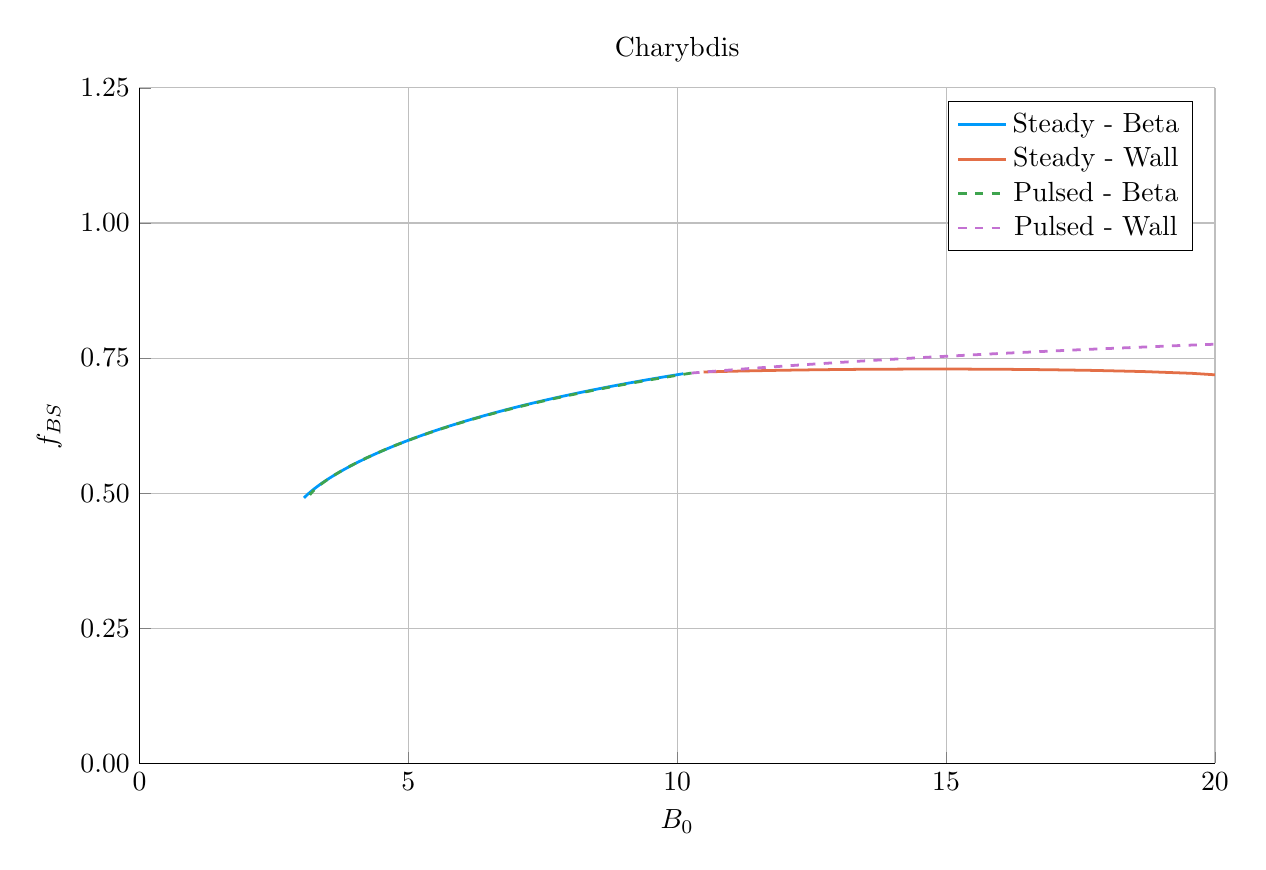
\begin{tikzpicture}[]
\begin{axis}[height = {101.6mm}, ylabel = {${f}_{BS}$}, title = {Charybdis}, xmin = {0.0}, xmax = {20.0}, ymax = {1.25}, xlabel = {${B}_{0}$}, {unbounded coords=jump, scaled x ticks = false, xticklabel style={rotate = 0}, xmajorgrids = true, xtick = {0.0,5.0,10.0,15.0,20.0}, xticklabels = {0,5,10,15,20}, xtick align = inside, axis lines* = left, scaled y ticks = false, yticklabel style={rotate = 0}, ymajorgrids = true, ytick = {0.0,0.25,0.5,0.75,1.0,1.25}, yticklabels = {0.00,0.25,0.50,0.75,1.00,1.25}, ytick align = inside, axis lines* = left,     xshift = 0.0mm,
    yshift = 0.0mm,
    axis background/.style={fill={rgb,1:red,1.00000000;green,1.00000000;blue,1.00000000}}
, colorbar style={title=}}, ymin = {0.0}, width = {152.4mm}]\addplot+ [color = {rgb,1:red,0.00000000;green,0.60560316;blue,0.97868012},
draw opacity=1.0,
line width=1,
solid,mark = none,
mark size = 2.0,
mark options = {
    color = {rgb,1:red,0.00000000;green,0.00000000;blue,0.00000000}, draw opacity = 1.0,
    fill = {rgb,1:red,0.00000000;green,0.60560316;blue,0.97868012}, fill opacity = 1.0,
    line width = 1,
    rotate = 0,
    solid
}]coordinates {
(10.112818033153026, 0.7210204864939177)
(9.722156888543116, 0.7146370182366134)
(9.357875603858393, 0.7083864126933084)
(9.017653755630063, 0.7022672660628055)
(8.6995124437054, 0.6962802592140539)
(8.401566530516865, 0.6904227919556637)
(8.122163706328223, 0.6846931203855893)
(7.859819415455661, 0.6790893709043329)
(7.613196557650265, 0.67360956295052)
(7.381088038653343, 0.6682516290962779)
(7.162401716104116, 0.6630134327794849)
(6.956147367527331, 0.6578927839230788)
(6.761425371986388, 0.6528874526668769)
(6.577416849463348, 0.6479951814148015)
(6.403375044688587, 0.6432136953797959)
(6.2386177769852695, 0.6385407117900744)
(6.0825208065966905, 0.6339739479091961)
(5.934511989185341, 0.6295111279665222)
(5.794066116682695, 0.6251499892035408)
(5.660700347012839, 0.6208882870235819)
(5.533970150598111, 0.6167237994278268)
(5.413465705416883, 0.612654330782363)
(5.298808685607224, 0.6086777150203906)
(5.189649392059402, 0.6047918182876691)
(5.085664187259174, 0.6009945411717122)
(4.986553195072601, 0.5972838205063521)
(4.892038235455667, 0.5936576308245715)
(4.801860966679364, 0.5901139854978271)
(4.7157812114040425, 0.5866509375997223)
(4.633575445956479, 0.5832665805277968)
(4.5550354347559185, 0.5799590484134715)
(4.479966994069385, 0.5767265163469188)
(4.408188871204256, 0.5735672004406611)
(4.33953172691477, 0.5704793577530769)
(4.273837210246432, 0.5674612860906418)
(4.210957116299974, 0.5645113237056368)
(4.15075261849161, 0.5616278489041633)
(4.0930935678432965, 0.5588092795776518)
(4.037857852672517, 0.5560540726695488)
(3.9849308127842145, 0.5533607235875209)
(3.9342047029103653, 0.5507277655703423)
(3.8855782007091695, 0.5481537690175585)
(3.838955955133626, 0.5456373407890682)
(3.7942481714200484, 0.5431771234809328)
(3.7513702293348077, 0.5407717946829491)
(3.710242331663442, 0.5384200662228671)
(3.6707891802306123, 0.5361206834015193)
(3.6329396770109583, 0.5338724242226064)
(3.5966266481325166, 0.5316740986203955)
(3.5617865887889004, 0.5295245476881729)
(3.5283594272686503, 0.5274226429099164)
(3.496288306480746, 0.5253672853972962)
(3.465519381509793, 0.523357405133857)
(3.4360016318699595, 0.521391960227916)
(3.4076866872513096, 0.519469936175524)
(3.380528665662031, 0.5175903451345877)
(3.3544840229690007, 0.515752225211106)
(3.3295114129297314, 0.5139546397582719)
(3.3055715568879336, 0.5121966766890691)
(3.2826271223788512, 0.5104774478028604)
(3.260642607548369, 0.5087960880501073)
(3.239584247604666, 0.5071517552692125)
(3.2194198921826622, 0.5055436287945424)
(3.2001189373344725, 0.5039709096043281)
(3.181652227422265, 0.5024328193399152)
(3.163991977015565, 0.5009285997975061)
(3.1471116955378684, 0.4994575123586322)
(3.130986116696265, 0.4980188374354915)
(3.115591132350856, 0.4966118739310214)
(3.1009037305081053, 0.49523593871353894)
(3.0869019371473265, 0.49389036610575116)
(3.0735647616124355, 0.4925745073879161)
(3.0608721453218655, 0.4912877303149199)
};
\addlegendentry{Steady - Beta}
\addplot+ [color = {rgb,1:red,0.88887350;green,0.43564919;blue,0.27812294},
draw opacity=1.0,
line width=1,
solid,mark = none,
mark size = 2.0,
mark options = {
    color = {rgb,1:red,0.00000000;green,0.00000000;blue,0.00000000}, draw opacity = 1.0,
    fill = {rgb,1:red,0.88887350;green,0.43564919;blue,0.27812294}, fill opacity = 1.0,
    line width = 1,
    rotate = 0,
    solid
}]coordinates {
(20.758867641064707, 0.7086877929835796)
(20.346250098246923, 0.7168022789486331)
(19.57104597888471, 0.7217497134740003)
(18.681781921115476, 0.7249695056379133)
(17.775790175980152, 0.7270845047632989)
(16.896654716492492, 0.7284340276383934)
(16.063927450323227, 0.7292257513380013)
(15.285557510665852, 0.7295982026655975)
(14.563500533069154, 0.7296487331947856)
(13.896568848875791, 0.7294482230480142)
(13.281970890030232, 0.7290496155282441)
(12.716170469467318, 0.728493234024972)
(12.195372283741088, 0.7278102698619938)
(11.715794270833433, 0.7270251605848495)
(11.273815669498969, 0.7261572607473546)
(10.866051794088186, 0.7252220436896863)
(10.489365023931143, 0.7242317330125791)
};
\addlegendentry{Steady - Wall}
\addplot+ [color = {rgb,1:red,0.24222430;green,0.64327509;blue,0.30444865},
draw opacity=1.0,
line width=1,
dashed,mark = none,
mark size = 2.0,
mark options = {
    color = {rgb,1:red,0.00000000;green,0.00000000;blue,0.00000000}, draw opacity = 1.0,
    fill = {rgb,1:red,0.24222430;green,0.64327509;blue,0.30444865}, fill opacity = 1.0,
    line width = 1,
    rotate = 0,
    solid
}]coordinates {
(10.26788634689966, 0.7223092996988955)
(9.953967652326213, 0.7173421457650607)
(9.567926244368271, 0.7109549304917827)
(9.207974394987358, 0.704700782459153)
(8.871841888699304, 0.6985789445752383)
(8.557505525932248, 0.6925884412510209)
(8.263156925406376, 0.6867281064999733)
(7.9871752024348766, 0.6809966091940381)
(7.728103682045175, 0.6753924756757733)
(7.484629973620137, 0.6699141100164039)
(7.255568856523303, 0.6645598121477955)
(7.039847526735421, 0.6593277940799372)
(6.836492834698909, 0.6542161943953472)
(6.644620209081183, 0.6492230911934739)
(6.463424013335149, 0.6443465136413796)
(6.2921691243175495, 0.6395844522716652)
(6.13018355681404, 0.6349348681547167)
(5.97685198655569, 0.6303957010676767)
(5.831610044919842, 0.6259648767156192)
(5.693939286027163, 0.6216403132173487)
(5.563362729090489, 0.617419926778885)
(5.439440906144732, 0.6133016367504772)
(5.321768347746793, 0.60928337008091)
(5.209970453003084, 0.6053630652695442)
(5.103700692769835, 0.6015386757890067)
(5.002638109938164, 0.5978081731386222)
(4.906485077678376, 0.5941695494871705)
(4.814965286571576, 0.590620819979065)
(4.727821933804548, 0.5871600247334057)
(4.644816091323922, 0.583785230567476)
(4.565725232806084, 0.5804945324731441)
(4.490341901840154, 0.5772860548715839)
(4.418472505906755, 0.5741579526691204)
(4.349936222622964, 0.571108412134701)
(4.284564006352339, 0.5681356516172873)
(4.222197684694192, 0.5652379221196283)
(4.162689135592264, 0.5624135077431643)
(4.105899536872315, 0.5596607260172779)
(4.051698680949713, 0.5569779281247673)
(3.9999643482627323, 0.5543634990341706)
(3.9505817337017928, 0.5518158575485668)
(3.903442920928527, 0.5493334562793774)
(3.858446400032002, 0.5469147815529699)
(3.8154966244515616, 0.5445583532569968)
(3.7745036035252744, 0.5422627246327709)
(3.7353825273991994, 0.5400264820193224)
(3.6980534213689746, 0.5378482445542797)
(3.6624408270205375, 0.5357266638362004)
(3.62847350780097, 0.5336604235525567)
(3.5960841768845415, 0.5316482390771937)
(3.565209245407392, 0.5296888570407133)
(3.5357885893311605, 0.527781054876968)
(3.5077653333614305, 0.5259236403485228)
(3.4810856504959875, 0.5241154510537358)
(3.4556985759109375, 0.5223553539178648)
(3.4315558340122845, 0.5206422446704141)
(3.408611677587535, 0.5189750473107426)
(3.3868227380888998, 0.5173527135638236)
(3.36614788616562, 0.5157742223278504)
(3.3465481016421226, 0.5142385791153044)
(3.327986352208224, 0.5127448154889249)
(3.3104274769652595, 0.5112919883802539)
(3.2938380965241474, 0.509879180087844)
(3.278186482171801, 0.5085054965688005)
(3.263442495132517, 0.5071700680038417)
(3.2495774839156075, 0.5058720476577763)
(3.236564206241785, 0.50461061142376)
(3.224376752844934, 0.5033849572563724)
(3.212990475972638, 0.502194304607974)
(3.2023819222517877, 0.5010378938690899)
(3.192528769611062, 0.499914985813462)
(3.1834097679780142, 0.49882486104841556)
(3.1750046834890777, 0.4977668194710788)
(3.1672942459724482, 0.4967401797310071)
};
\addlegendentry{Pulsed - Beta}
\addplot+ [color = {rgb,1:red,0.76444018;green,0.44411178;blue,0.82429754},
draw opacity=1.0,
line width=1,
dashed,mark = none,
mark size = 2.0,
mark options = {
    color = {rgb,1:red,0.00000000;green,0.00000000;blue,0.00000000}, draw opacity = 1.0,
    fill = {rgb,1:red,0.76444018;green,0.44411178;blue,0.82429754}, fill opacity = 1.0,
    line width = 1,
    rotate = 0,
    solid
}]coordinates {
(48.990476413653056, 0.836749542460291)
(42.83950920694117, 0.8284827071479798)
(37.687790427214495, 0.8202912319532255)
(33.33937742845888, 0.8121855711018737)
(29.64296398154308, 0.8041747843540442)
(26.48039367255613, 0.7962666686333785)
(23.758442882319894, 0.7884678803807476)
(21.402860298405816, 0.780784048608438)
(19.353987387634486, 0.7732198788517932)
(17.563502020363714, 0.7657792483576302)
(15.991970371213752, 0.7584652929710556)
(14.606987499719377, 0.7512804862003557)
(13.381751501116137, 0.7442267110066104)
(12.293960329570087, 0.7373053248499966)
(11.32495111804522, 0.7305172185244015)
(10.459023415380802, 0.7238628692935026)
(10.26788634689966, 0.7223092996988955)
};
\addlegendentry{Pulsed - Wall}
\end{axis}

\end{tikzpicture}

    \end{adjustbox}
        \caption{Charybdis}
    \end{subfigure}
    \hfill
    \begin{subfigure}[t]{0.45\textwidth}
        \centering
    \begin{adjustbox}{width=\textwidth}
      \Large
      \begin{tikzpicture}[]
\begin{axis}[height = {101.6mm}, ylabel = {${f}_{BS}$}, title = {Proteus}, xmin = {0.0}, xmax = {20.0}, ymax = {1.25}, xlabel = {${B}_{0}$}, {unbounded coords=jump, scaled x ticks = false, xticklabel style={rotate = 0}, xmajorgrids = true, xtick = {0.0,5.0,10.0,15.0,20.0}, xticklabels = {0,5,10,15,20}, xtick align = inside, axis lines* = left, scaled y ticks = false, yticklabel style={rotate = 0}, ymajorgrids = true, ytick = {0.0,0.25,0.5,0.75,1.0,1.25}, yticklabels = {0.00,0.25,0.50,0.75,1.00,1.25}, ytick align = inside, axis lines* = left,     xshift = 0.0mm,
    yshift = 0.0mm,
    axis background/.style={fill={rgb,1:red,1.00000000;green,1.00000000;blue,1.00000000}}
, colorbar style={title=}}, ymin = {0.0}, width = {152.4mm}]\addplot+ [color = {rgb,1:red,0.00000000;green,0.60560316;blue,0.97868012},
draw opacity=1.0,
line width=1,
solid,mark = none,
mark size = 2.0,
mark options = {
    color = {rgb,1:red,0.00000000;green,0.00000000;blue,0.00000000}, draw opacity = 1.0,
    fill = {rgb,1:red,0.00000000;green,0.60560316;blue,0.97868012}, fill opacity = 1.0,
    line width = 1,
    rotate = 0,
    solid
}]coordinates {
(4.658732060637907, 0.03374327843251104)
(4.211109766361548, 0.04705745700285543)
(3.9293920326356777, 0.061421617822527384)
(3.7651903683456465, 0.07588846730345673)
(3.6776039543745567, 0.08999143545083153)
(3.6402437753208394, 0.1035293038539849)
(3.6366994671255806, 0.11643477465969046)
(3.656621534643579, 0.12870407540884737)
(3.693300156736026, 0.14036149397161052)
(3.7422515017241134, 0.15144212823106107)
(3.865532743079537, 0.17202317779275975)
(3.936096932264377, 0.1815947312397854)
(4.010907188015084, 0.1907298222625134)
(4.089072356933184, 0.19945693150761834)
(4.169903401491354, 0.20780181554781404)
(4.252857906625248, 0.21578777589683956)
(4.337501757261618, 0.2234359357663511)
(4.42348218754058, 0.23076549870092802)
(4.5983381267510195, 0.24453740840266724)
(4.686766232902671, 0.25101050275030934)
(4.775618142770625, 0.2572268217878506)
(4.864743502376605, 0.26319889521809087)
(4.927312314219091, 0.26724594989061395)
};
\addlegendentry{Pulsed - Kink}
\addplot+ [color = {rgb,1:red,0.88887350;green,0.43564919;blue,0.27812294},
draw opacity=1.0,
line width=1,
solid,mark = none,
mark size = 2.0,
mark options = {
    color = {rgb,1:red,0.00000000;green,0.00000000;blue,0.00000000}, draw opacity = 1.0,
    fill = {rgb,1:red,0.88887350;green,0.43564919;blue,0.27812294}, fill opacity = 1.0,
    line width = 1,
    rotate = 0,
    solid
}]coordinates {
(4.927312314219091, 0.26724594989061395)
(4.984545814413324, 0.2691891196965451)
(5.17452482724068, 0.275516623793244)
(5.362091669637646, 0.2815863664246872)
(5.54700293215903, 0.2874061454494217)
(5.729042482638278, 0.2929837150433957)
(5.908022832274664, 0.29832680692607144)
(6.083785777786694, 0.30344314004485806)
(6.256202341425288, 0.3083404200555057)
(6.324169421042356, 0.3102386318468015)
};
\addlegendentry{Pulsed - Beta}
\addplot+ [color = {rgb,1:red,0.24222430;green,0.64327509;blue,0.30444865},
draw opacity=1.0,
line width=1,
solid,mark = none,
mark size = 2.0,
mark options = {
    color = {rgb,1:red,0.00000000;green,0.00000000;blue,0.00000000}, draw opacity = 1.0,
    fill = {rgb,1:red,0.24222430;green,0.64327509;blue,0.30444865}, fill opacity = 1.0,
    line width = 1,
    rotate = 0,
    solid
}]coordinates {
(6.324169421042356, 0.3102386318468015)
(6.727338549778396, 0.314904725402431)
(7.320469048424473, 0.32166792307902226)
(7.835746509376305, 0.32748269750323933)
(8.290245520072391, 0.33258608250843447)
(8.696162676727877, 0.3371327582242265)
(9.0624397222742, 0.3412289740912578)
(9.395798186463841, 0.34495090965414)
(9.701405747258567, 0.3483551844586761)
(10.244760202900984, 0.3543749911810046)
(10.930275827723788, 0.36185386392937047)
(11.131878682735255, 0.36401313377263034)
(11.50278450645086, 0.36791636281758366)
(11.83715172742864, 0.3713365223675564)
(11.992609772603878, 0.3728873208216849)
(12.141110720831467, 0.37434168635049264)
};
\addlegendentry{Pulsed - Wall}
\end{axis}

\end{tikzpicture}

    \end{adjustbox}
        \caption{Proteus}
    \end{subfigure}
    \hfill \hfill ~\\ ~\\ ~\\ ~\\
    \hfill
    \begin{subfigure}[t]{0.45\textwidth}
        \centering
    \begin{adjustbox}{width=\textwidth}
      \Large
      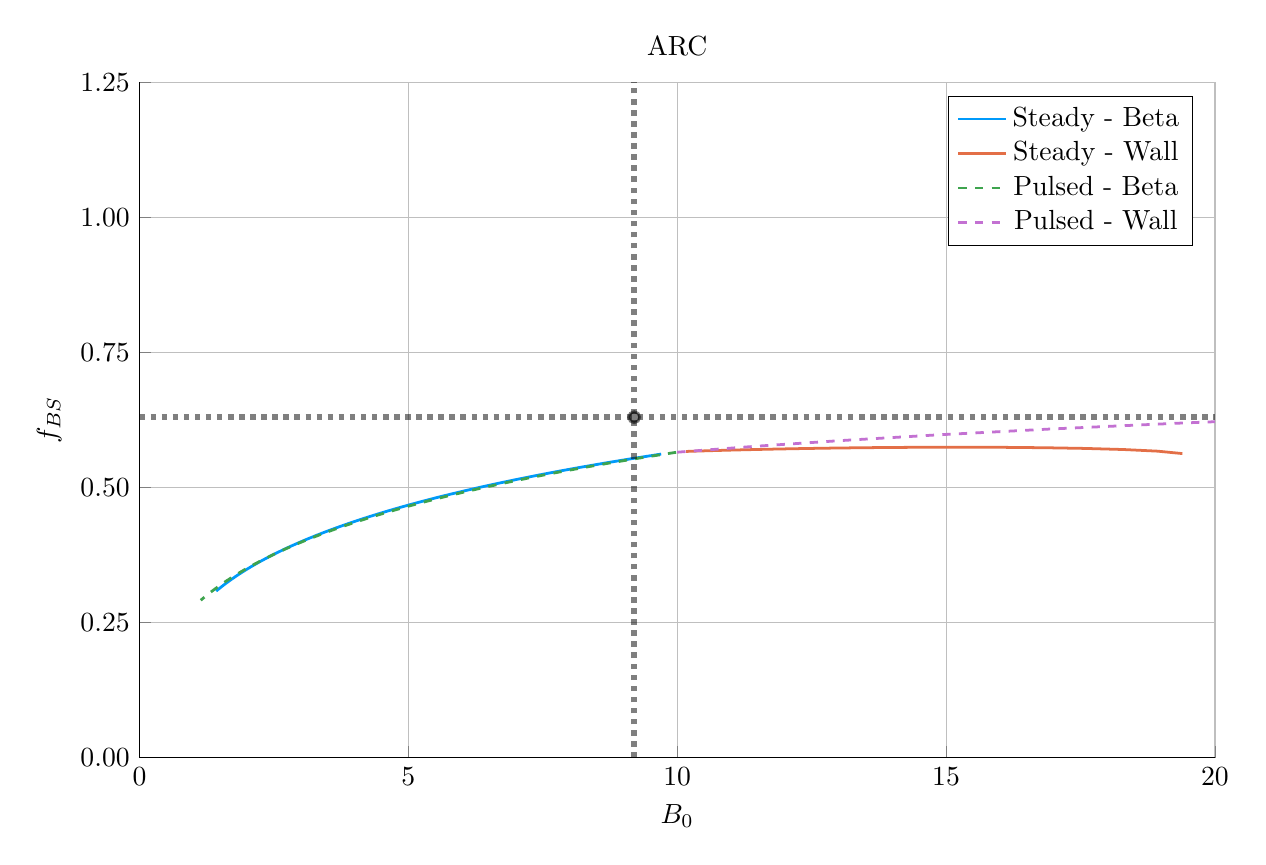
\begin{tikzpicture}[]
\begin{axis}[height = {101.6mm}, ylabel = {${f}_{BS}$}, title = {ARC}, xmin = {0.0}, xmax = {20.0}, ymax = {1.25}, xlabel = {${B}_{0}$}, {unbounded coords=jump, scaled x ticks = false, xticklabel style={rotate = 0}, xmajorgrids = true, xtick = {0.0,5.0,10.0,15.0,20.0}, xticklabels = {0,5,10,15,20}, xtick align = inside, axis lines* = left, scaled y ticks = false, yticklabel style={rotate = 0}, ymajorgrids = true, ytick = {0.0,0.25,0.5,0.75,1.0,1.25}, yticklabels = {0.00,0.25,0.50,0.75,1.00,1.25}, ytick align = inside, axis lines* = left,     xshift = 0.0mm,
    yshift = 0.0mm,
    axis background/.style={fill={rgb,1:red,1.00000000;green,1.00000000;blue,1.00000000}}
, colorbar style={title=}}, ymin = {0.0}, width = {152.4mm}]\addplot+ [color = {rgb,1:red,0.00000000;green,0.60560316;blue,0.97868012},
draw opacity=1.0,
line width=1,
solid,mark = none,
mark size = 2.0,
mark options = {
    color = {rgb,1:red,0.00000000;green,0.00000000;blue,0.00000000}, draw opacity = 1.0,
    fill = {rgb,1:red,0.00000000;green,0.60560316;blue,0.97868012}, fill opacity = 1.0,
    line width = 1,
    rotate = 0,
    solid
}]coordinates {
(9.701206080853105, 0.5617985361890832)
(9.162315904693079, 0.5534422734511444)
(8.664301107137337, 0.5453002015966304)
(8.203576462497304, 0.5373715237609187)
(7.776718537485166, 0.5296505594600077)
(7.380720231870917, 0.5221327240909955)
(7.012886014999712, 0.5148133533264904)
(6.670795005901889, 0.5076877327676947)
(6.352268997292712, 0.5007511235730646)
(6.055344682097163, 0.49399878452544604)
(5.778249464564785, 0.4874259909515555)
(5.519380338856715, 0.4810280508632015)
(5.2772854007125325, 0.47480031864954747)
(5.050647625972996, 0.468738206613593)
(4.838270606140816, 0.46283719461361283)
(4.639065978019038, 0.45709283804121914)
(4.4520423235376105, 0.45150077434170793)
(4.276295348572609, 0.4460567282590674)
(4.110999177018484, 0.44075651596731874)
(3.9553986195015125, 0.43559604823132275)
(3.8088022956698633, 0.43057133272373177)
(3.6705765055641186, 0.42567847561009164)
(3.54013975965751, 0.42091368250105043)
(3.4169578891619192, 0.4162732588590562)
(3.30053966845824, 0.41175360993660254)
(3.1904328903033052, 0.40735124031396425)
(3.086220842019516, 0.4030627530962233)
(2.9875191373772063, 0.3988848488222173)
(2.8939728644914635, 0.3948143241316363)
(2.8052540149097247, 0.39084807023084916)
(2.7210591632720242, 0.38698307119303055)
(2.6411073705789065, 0.38321640212371255)
(2.565138287279709, 0.3795452272189691)
(2.492910435164382, 0.37596679773995195)
(2.4241996494611984, 0.37247844992443246)
(2.3587976646588236, 0.36907760285328395)
(2.296510829425685, 0.36576175628743024)
(2.237158937627476, 0.36252848848868546)
(2.180574163874242, 0.3593754540360099)
(2.126600093288366, 0.3563003816470909)
(2.075090836295778, 0.35330107201367594)
(2.0259102202234582, 0.35037539565782555)
(1.978931050353818, 0.34752129081511496)
(1.9340344338545452, 0.3447367613498354)
(1.8911091606836798, 0.3420198747063713)
(1.8500511361739687, 0.3393687599001731)
(1.8107628605384507, 0.3367816055510836)
(1.773152951016952, 0.33425665796118464)
(1.7371357028100902, 0.33179221923883906)
(1.7026306853269466, 0.3293866454701516)
(1.6695623706125668, 0.3270383449386928)
(1.6378597911249178, 0.3247457763940071)
(1.607456224302725, 0.3225074473691236)
(1.5782889016090462, 0.32032191254706976)
(1.5502987399539199, 0.31818777217614846)
(1.5234300935954943, 0.3161036705335871)
(1.4976305247952577, 0.31406829443699913)
(1.4728505916614916, 0.3120803718029801)
(1.4490436517578602, 0.3101386702520509)
(1.4261656801829077, 0.30824199575908484)
};
\addlegendentry{Steady - Beta}
\addplot+ [color = {rgb,1:red,0.88887350;green,0.43564919;blue,0.27812294},
draw opacity=1.0,
line width=1,
solid,mark = none,
mark size = 2.0,
mark options = {
    color = {rgb,1:red,0.00000000;green,0.00000000;blue,0.00000000}, draw opacity = 1.0,
    fill = {rgb,1:red,0.88887350;green,0.43564919;blue,0.27812294}, fill opacity = 1.0,
    line width = 1,
    rotate = 0,
    solid
}]coordinates {
(19.394007482712425, 0.5626988342140414)
(18.932196567189358, 0.5671974126141779)
(18.296989378345195, 0.5702172271507213)
(17.587029315408756, 0.5722409138271746)
(16.847882407994106, 0.5735084646592641)
(16.111374502564406, 0.5742120779196618)
(15.396027314547156, 0.5744872159421819)
(14.710952688793137, 0.5744238623033726)
(14.06168447794857, 0.5740960556207445)
(13.450465418483889, 0.5735594327508525)
(12.877644538645335, 0.5728574304868504)
(12.342394470642008, 0.5720242976430745)
(11.843182246608265, 0.5710872464853384)
(11.376441269625893, 0.5700535966602547)
(10.944966372727551, 0.5689841327881735)
(10.541663878705513, 0.5678496538517193)
(10.165908182236457, 0.5666749328229757)
};
\addlegendentry{Steady - Wall}
\addplot+ [color = {rgb,1:red,0.24222430;green,0.64327509;blue,0.30444865},
draw opacity=1.0,
line width=1,
dashed,mark = none,
mark size = 2.0,
mark options = {
    color = {rgb,1:red,0.00000000;green,0.00000000;blue,0.00000000}, draw opacity = 1.0,
    fill = {rgb,1:red,0.24222430;green,0.64327509;blue,0.30444865}, fill opacity = 1.0,
    line width = 1,
    rotate = 0,
    solid
}]coordinates {
(9.980483622051658, 0.5650608431663754)
(9.392786903460065, 0.5559661724011671)
(8.79273598103983, 0.5461307467124767)
(8.23820290909994, 0.5364900413795539)
(7.725182218401588, 0.5270433245554992)
(7.250078106370205, 0.5177895246779806)
(6.80965553466646, 0.5087272673879922)
(6.400998063035608, 0.4998549082898422)
(6.0214713600430425, 0.4911705618331852)
(5.668691517461799, 0.48267212656163294)
(5.340497445229901, 0.47435730693753847)
(5.034926745580058, 0.466223631918386)
(4.750194564008521, 0.45826847042635843)
(4.484674995755211, 0.4504890438186267)
(4.236884692979903, 0.4428824354312153)
(4.00546837264544, 0.43544559723298737)
(3.7891859704718387, 0.42817535358744846)
(3.5869012239550364, 0.421068402076909)
(3.3975714987448393, 0.4141213112942482)
(3.2202386987489797, 0.4073305154489277)
(3.0540211220494466, 0.40069230556225255)
(2.8981061427709687, 0.3942028169364579)
(2.7517436139566023, 0.38785801246536006)
(2.6142398986781377, 0.38165366120017824)
(2.4849524463010138, 0.37558531137706375)
(2.363284838174807, 0.3696482568306765)
(2.248682232019848, 0.363837495327903)
(2.140627136740878, 0.35814767680897164)
(2.038635448877246, 0.3525730387458944)
(1.9422526775794744, 0.3471073247061474)
(1.8510502754751532, 0.3417436805619704)
(1.7646219756564088, 0.3364745203191482)
(1.6825800061969869, 0.3312913497640341)
(1.6045510059627948, 0.32618453020192045)
(1.53017138625397, 0.3211429549856907)
(1.4590817483192686, 0.31615359554075645)
(1.3909197311384796, 0.31120084582704777)
(1.3253102336217724, 0.3062655437505664)
(1.261851128383913, 0.3013234514127004)
(1.20009089049112, 0.29634277859379204)
(1.1394908096975784, 0.291279896704588)
};
\addlegendentry{Pulsed - Beta}
\addplot+ [color = {rgb,1:red,0.76444018;green,0.44411178;blue,0.82429754},
draw opacity=1.0,
line width=1,
dashed,mark = none,
mark size = 2.0,
mark options = {
    color = {rgb,1:red,0.00000000;green,0.00000000;blue,0.00000000}, draw opacity = 1.0,
    fill = {rgb,1:red,0.76444018;green,0.44411178;blue,0.82429754}, fill opacity = 1.0,
    line width = 1,
    rotate = 0,
    solid
}]coordinates {
(29.27715761652869, 0.6531372657200456)
(25.4410619834368, 0.6415971079030305)
(22.158819835998365, 0.6302343721213154)
(19.342453256965573, 0.6190539199503469)
(16.919364280634177, 0.6080596927511532)
(14.829378672669455, 0.597254804677281)
(13.022412368922526, 0.5866416275674396)
(11.456617692058645, 0.5762218683352907)
(10.096901921254785, 0.565996639419092)
(9.980483622051658, 0.5650608431663754)
};
\addlegendentry{Pulsed - Wall}
\addplot+ [color = {rgb,1:red,0.00000000;green,0.00000000;blue,0.00000000},
draw opacity=0.5,
line width=2,
dotted,mark = none,
mark size = 2.0,
mark options = {
    color = {rgb,1:red,0.00000000;green,0.00000000;blue,0.00000000}, draw opacity = 0.5,
    fill = {rgb,1:red,0.00000000;green,0.00000000;blue,0.00000000}, fill opacity = 0.5,
    line width = 1,
    rotate = 0,
    solid
},forget plot]coordinates {
(0.0, 0.63)
(20.0, 0.63)
};
\addplot+ [color = {rgb,1:red,0.00000000;green,0.00000000;blue,0.00000000},
draw opacity=0.5,
line width=2,
dotted,mark = none,
mark size = 2.0,
mark options = {
    color = {rgb,1:red,0.00000000;green,0.00000000;blue,0.00000000}, draw opacity = 0.5,
    fill = {rgb,1:red,0.00000000;green,0.00000000;blue,0.00000000}, fill opacity = 0.5,
    line width = 1,
    rotate = 0,
    solid
},forget plot]coordinates {
(9.2, 0.0)
(9.2, 1.25)
};
\addplot+[draw=none, color = {rgb,1:red,0.00000000;green,0.00000000;blue,0.00000000},
draw opacity=0.5,
line width=0,
solid,mark = *,
mark size = 2.0,
mark options = {
    color = {rgb,1:red,0.00000000;green,0.00000000;blue,0.00000000}, draw opacity = 0.5,
    fill = {rgb,1:red,0.00000000;green,0.00000000;blue,0.00000000}, fill opacity = 0.5,
    line width = 1,
    rotate = 0,
    solid
},forget plot] coordinates {
(9.2, 0.63)
};
\end{axis}

\end{tikzpicture}

    \end{adjustbox}
        \caption{ARC}
    \end{subfigure}
    \hfill
    \begin{subfigure}[t]{0.45\textwidth}
        \centering
    \begin{adjustbox}{width=\textwidth}
      \Large
      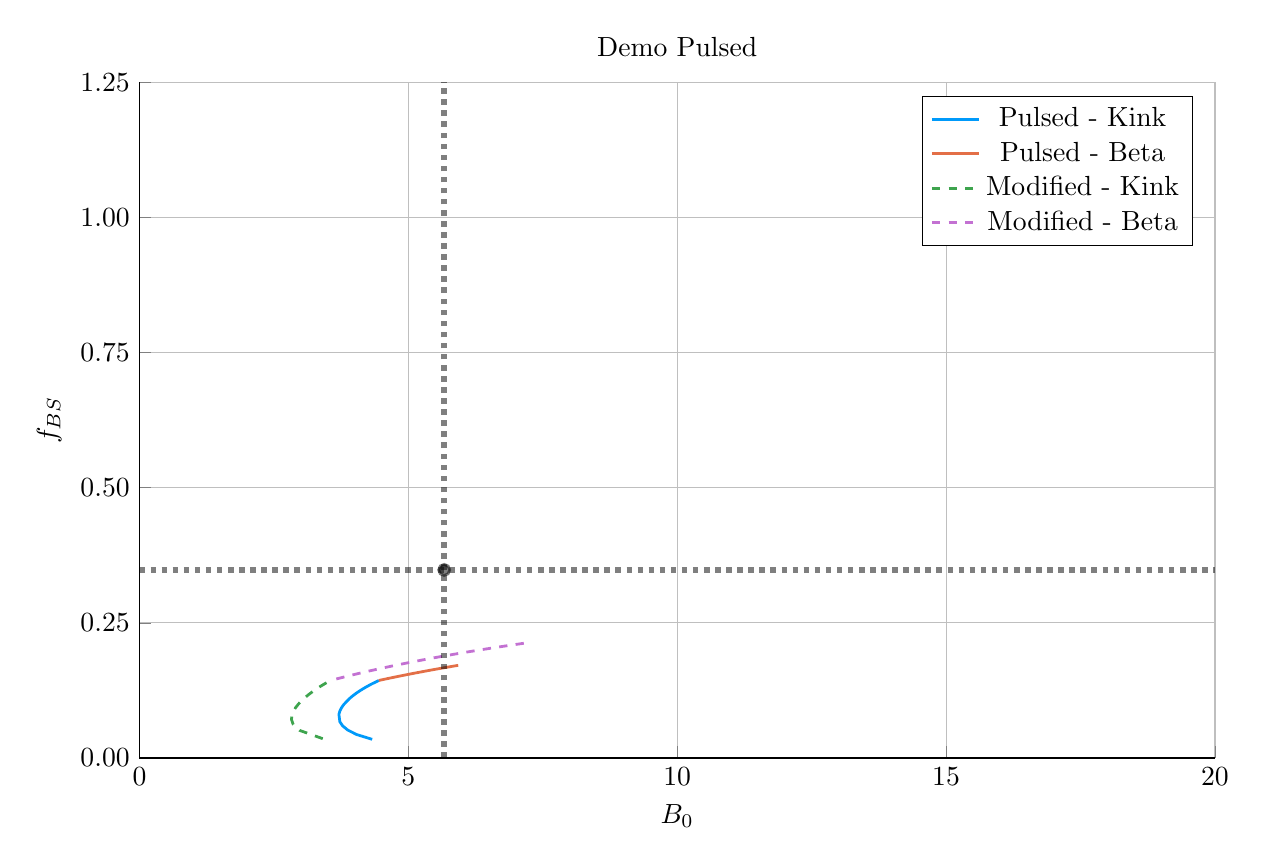
\begin{tikzpicture}[]
\begin{axis}[height = {101.6mm}, ylabel = {${f}_{BS}$}, title = {Demo Pulsed}, xmin = {0.0}, xmax = {20.0}, ymax = {1.25}, xlabel = {${B}_{0}$}, {unbounded coords=jump, scaled x ticks = false, xticklabel style={rotate = 0}, xmajorgrids = true, xtick = {0.0,5.0,10.0,15.0,20.0}, xticklabels = {0,5,10,15,20}, xtick align = inside, axis lines* = left, scaled y ticks = false, yticklabel style={rotate = 0}, ymajorgrids = true, ytick = {0.0,0.25,0.5,0.75,1.0,1.25}, yticklabels = {0.00,0.25,0.50,0.75,1.00,1.25}, ytick align = inside, axis lines* = left,     xshift = 0.0mm,
    yshift = 0.0mm,
    axis background/.style={fill={rgb,1:red,1.00000000;green,1.00000000;blue,1.00000000}}
, colorbar style={title=}}, ymin = {0.0}, width = {152.4mm}]\addplot+ [color = {rgb,1:red,0.00000000;green,0.60560316;blue,0.97868012},
draw opacity=1.0,
line width=1,
solid,mark = none,
mark size = 2.0,
mark options = {
    color = {rgb,1:red,0.00000000;green,0.00000000;blue,0.00000000}, draw opacity = 1.0,
    fill = {rgb,1:red,0.00000000;green,0.60560316;blue,0.97868012}, fill opacity = 1.0,
    line width = 1,
    rotate = 0,
    solid
}]coordinates {
(4.327031075670194, 0.034480220241779755)
(4.038214026054326, 0.04336283531530908)
(3.8713719163129245, 0.051749529009171916)
(3.7758613845615545, 0.059658701796857776)
(3.7257856761317214, 0.06712097568220785)
(3.7090473695925437, 0.0808421993426635)
(3.727711597554826, 0.08716725879257335)
(3.7586131667481433, 0.0931751078928838)
(3.799052518631718, 0.09889195764117985)
(3.901290136389271, 0.10954369660908773)
(3.960577465316514, 0.114517980761529)
(4.0241209645210345, 0.119280610932012)
(4.0912717805663785, 0.12384638359682056)
(4.161514602943343, 0.12822856511510325)
(4.2344343960723005, 0.13243908708020224)
(4.309692554546368, 0.13648871500745674)
(4.450417240491067, 0.1434138491653015)
};
\addlegendentry{Pulsed - Kink}
\addplot+ [color = {rgb,1:red,0.88887350;green,0.43564919;blue,0.27812294},
draw opacity=1.0,
line width=1,
solid,mark = none,
mark size = 2.0,
mark options = {
    color = {rgb,1:red,0.00000000;green,0.00000000;blue,0.00000000}, draw opacity = 1.0,
    fill = {rgb,1:red,0.88887350;green,0.43564919;blue,0.27812294}, fill opacity = 1.0,
    line width = 1,
    rotate = 0,
    solid
}]coordinates {
(4.450417240491067, 0.1434138491653015)
(4.490148631384312, 0.14427095547870222)
(4.692490181445514, 0.148534819690196)
(4.8960344619053355, 0.15266171022829186)
(5.100651132702229, 0.15665692218118474)
(5.306202822090688, 0.16052534839697072)
(5.512545696627038, 0.16427151549651184)
(5.719530043226767, 0.167899617223133)
(5.927000883375481, 0.17141354535481249)
};
\addlegendentry{Pulsed - Beta}
\addplot+ [color = {rgb,1:red,0.24222430;green,0.64327509;blue,0.30444865},
draw opacity=1.0,
line width=1,
dashed,mark = none,
mark size = 2.0,
mark options = {
    color = {rgb,1:red,0.00000000;green,0.00000000;blue,0.00000000}, draw opacity = 1.0,
    fill = {rgb,1:red,0.24222430;green,0.64327509;blue,0.30444865}, fill opacity = 1.0,
    line width = 1,
    rotate = 0,
    solid
}]coordinates {
(3.4087424183072135, 0.03565362214144275)
(2.977074181068944, 0.05106869132768493)
(2.8592500074202523, 0.06190160489502012)
(2.827199220063259, 0.07097613389666015)
(2.8339789008667826, 0.07904290793331036)
(2.862412302880871, 0.08642154144971413)
(2.9044598258085443, 0.0932807064240353)
(2.95577893007882, 0.09972186873701357)
(3.0137895352525907, 0.1058118766340181)
(3.076849710218805, 0.11159786725788115)
(3.1438583711612704, 0.11711488562329275)
(3.214045733980633, 0.1223901103527317)
(3.2868548955983727, 0.1274453502910665)
(3.361871149981842, 0.13229859644020936)
(3.4387778750377818, 0.13696502830291482)
(3.5173279629378453, 0.14145769045254009)
};
\addlegendentry{Modified - Kink}
\addplot+ [color = {rgb,1:red,0.76444018;green,0.44411178;blue,0.82429754},
draw opacity=1.0,
line width=1,
dashed,mark = none,
mark size = 2.0,
mark options = {
    color = {rgb,1:red,0.00000000;green,0.00000000;blue,0.00000000}, draw opacity = 1.0,
    fill = {rgb,1:red,0.76444018;green,0.44411178;blue,0.82429754}, fill opacity = 1.0,
    line width = 1,
    rotate = 0,
    solid
}]coordinates {
(3.6607028750648505, 0.1462118278958435)
(3.8574448036470477, 0.1511528062974465)
(4.056375867871351, 0.1559437323926086)
(4.257366397480293, 0.1605907484668563)
(4.460279103534801, 0.16509942452449394)
(4.664969389370631, 0.16947483662528415)
(4.871285596007394, 0.1737216290094361)
(5.07906923307514, 0.17784406463401414)
(5.288155233306219, 0.18184606732639355)
(5.498372259673351, 0.18573125781451202)
(5.709543087166185, 0.18950298521990852)
(5.921485076209294, 0.19316435517575725)
(6.134010749367255, 0.19671825537378382)
(6.346928478632384, 0.200167379124604)
(6.560043285872518, 0.2035142473323563)
(6.773157754368795, 0.20676122915263437)
(6.986073044284746, 0.20991056148112272)
(7.198590001107076, 0.2129643673902369)
};
\addlegendentry{Modified - Beta}
\addplot+ [color = {rgb,1:red,0.00000000;green,0.00000000;blue,0.00000000},
draw opacity=0.5,
line width=2,
dotted,mark = none,
mark size = 2.0,
mark options = {
    color = {rgb,1:red,0.00000000;green,0.00000000;blue,0.00000000}, draw opacity = 0.5,
    fill = {rgb,1:red,0.00000000;green,0.00000000;blue,0.00000000}, fill opacity = 0.5,
    line width = 1,
    rotate = 0,
    solid
},forget plot]coordinates {
(0.0, 0.348)
(20.0, 0.348)
};
\addplot+ [color = {rgb,1:red,0.00000000;green,0.00000000;blue,0.00000000},
draw opacity=0.5,
line width=2,
dotted,mark = none,
mark size = 2.0,
mark options = {
    color = {rgb,1:red,0.00000000;green,0.00000000;blue,0.00000000}, draw opacity = 0.5,
    fill = {rgb,1:red,0.00000000;green,0.00000000;blue,0.00000000}, fill opacity = 0.5,
    line width = 1,
    rotate = 0,
    solid
},forget plot]coordinates {
(5.667, 0.0)
(5.667, 1.25)
};
\addplot+[draw=none, color = {rgb,1:red,0.00000000;green,0.00000000;blue,0.00000000},
draw opacity=0.5,
line width=0,
solid,mark = *,
mark size = 2.0,
mark options = {
    color = {rgb,1:red,0.00000000;green,0.00000000;blue,0.00000000}, draw opacity = 0.5,
    fill = {rgb,1:red,0.00000000;green,0.00000000;blue,0.00000000}, fill opacity = 0.5,
    line width = 1,
    rotate = 0,
    solid
},forget plot] coordinates {
(5.667, 0.348)
};
\end{axis}

\end{tikzpicture}

    \end{adjustbox}
        \caption{DEMO Pulsed}
    \end{subfigure}
    \hfill \hfill ~\\ ~\\ ~\\ ~\\
    \hfill
    \begin{subfigure}[t]{0.45\textwidth}
        \centering
    \begin{adjustbox}{width=\textwidth}
      \Large
      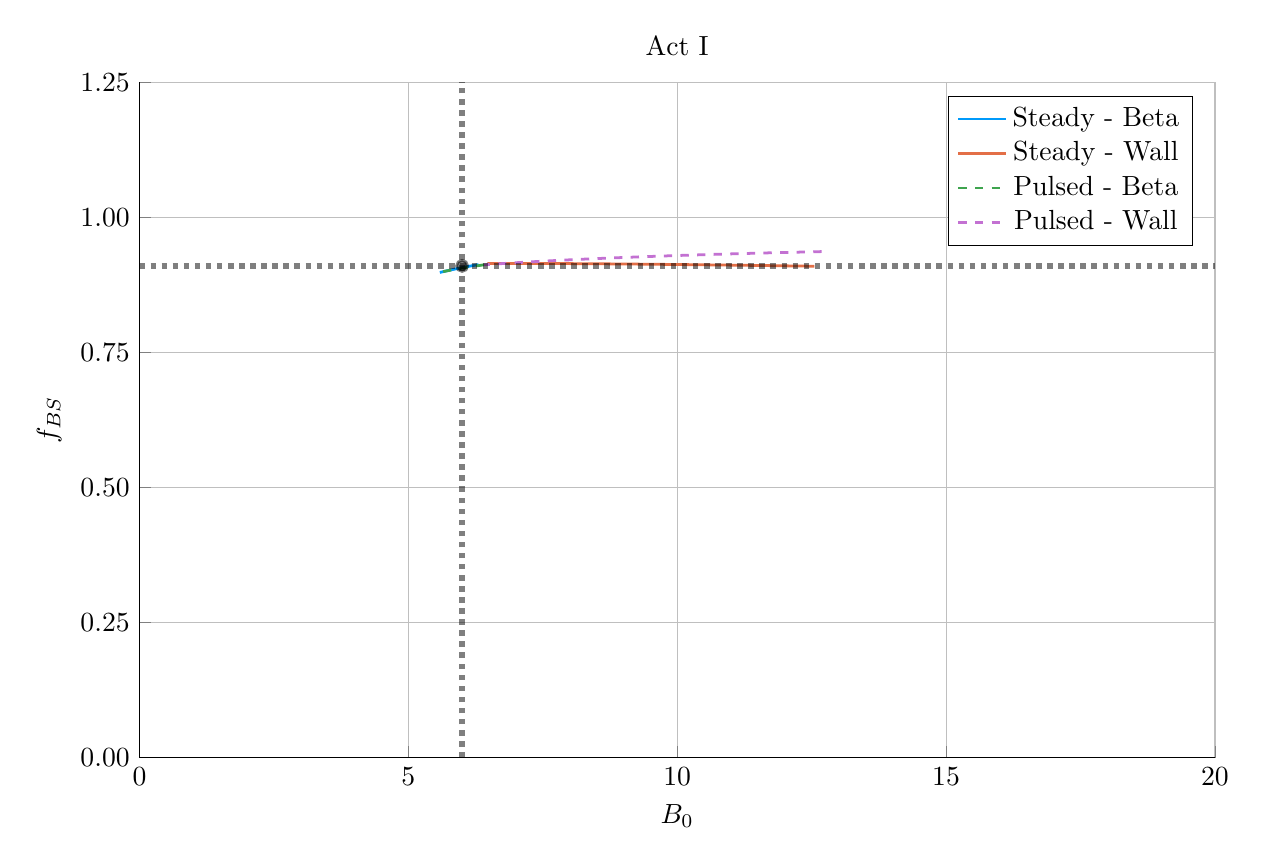
\begin{tikzpicture}[]
\begin{axis}[height = {101.6mm}, ylabel = {${f}_{BS}$}, title = {Act I}, xmin = {0.0}, xmax = {20.0}, ymax = {1.25}, xlabel = {${B}_{0}$}, {unbounded coords=jump, scaled x ticks = false, xticklabel style={rotate = 0}, xmajorgrids = true, xtick = {0.0,5.0,10.0,15.0,20.0}, xticklabels = {0,5,10,15,20}, xtick align = inside, axis lines* = left, scaled y ticks = false, yticklabel style={rotate = 0}, ymajorgrids = true, ytick = {0.0,0.25,0.5,0.75,1.0,1.25}, yticklabels = {0.00,0.25,0.50,0.75,1.00,1.25}, ytick align = inside, axis lines* = left,     xshift = 0.0mm,
    yshift = 0.0mm,
    axis background/.style={fill={rgb,1:red,1.00000000;green,1.00000000;blue,1.00000000}}
, colorbar style={title=}}, ymin = {0.0}, width = {152.4mm}]\addplot+ [color = {rgb,1:red,0.00000000;green,0.60560316;blue,0.97868012},
draw opacity=1.0,
line width=1,
solid,mark = none,
mark size = 2.0,
mark options = {
    color = {rgb,1:red,0.00000000;green,0.00000000;blue,0.00000000}, draw opacity = 1.0,
    fill = {rgb,1:red,0.00000000;green,0.60560316;blue,0.97868012}, fill opacity = 1.0,
    line width = 1,
    rotate = 0,
    solid
}]coordinates {
(6.30336807958207, 0.9124100954141464)
(6.162193069273141, 0.909925995406466)
(6.030717178404645, 0.9074680389222504)
(5.908065509576601, 0.9050369759461111)
(5.793464904530972, 0.9026334557593052)
(5.686229631357383, 0.900258028969911)
(5.585749511271037, 0.8979111563715388)
};
\addlegendentry{Steady - Beta}
\addplot+ [color = {rgb,1:red,0.88887350;green,0.43564919;blue,0.27812294},
draw opacity=1.0,
line width=1,
solid,mark = none,
mark size = 2.0,
mark options = {
    color = {rgb,1:red,0.00000000;green,0.00000000;blue,0.00000000}, draw opacity = 1.0,
    fill = {rgb,1:red,0.88887350;green,0.43564919;blue,0.27812294}, fill opacity = 1.0,
    line width = 1,
    rotate = 0,
    solid
}]coordinates {
(12.549536249695134, 0.9093812710629334)
(11.658754653696462, 0.9106086170053282)
(10.883719833507003, 0.9115889186790606)
(10.206258129789394, 0.9123717660963346)
(9.611335769312953, 0.912994317290827)
(9.086446934250878, 0.9134834010438713)
(8.62129895070743, 0.9138603988257706)
(8.207216040989662, 0.9141393102674468)
(7.837119555085499, 0.9143335795079951)
(7.505047858717157, 0.9144531084452595)
(7.20604322925957, 0.914506893061148)
(6.935884710193303, 0.9145014954975229)
(6.691016583192173, 0.9144427981592678)
(6.468415485086983, 0.9143358286457826)
};
\addlegendentry{Steady - Wall}
\addplot+ [color = {rgb,1:red,0.24222430;green,0.64327509;blue,0.30444865},
draw opacity=1.0,
line width=1,
dashed,mark = none,
mark size = 2.0,
mark options = {
    color = {rgb,1:red,0.00000000;green,0.00000000;blue,0.00000000}, draw opacity = 1.0,
    fill = {rgb,1:red,0.24222430;green,0.64327509;blue,0.30444865}, fill opacity = 1.0,
    line width = 1,
    rotate = 0,
    solid
}]coordinates {
(6.408263337806559, 0.9120300316986245)
(6.408263337806564, 0.9120300316986246)
(6.385466513301022, 0.9117124326684914)
(6.245492502072912, 0.909694750915225)
(6.116010320461132, 0.9077169851916397)
(5.9960421481916395, 0.9057789426538279)
(5.884727159112828, 0.9038803642916121)
(5.781304768121868, 0.9020209333516035)
(5.685100648450046, 0.9002002829223104)
(5.595515000321003, 0.89841800272554)
};
\addlegendentry{Pulsed - Beta}
\addplot+ [color = {rgb,1:red,0.76444018;green,0.44411178;blue,0.82429754},
draw opacity=1.0,
line width=1,
dashed,mark = none,
mark size = 2.0,
mark options = {
    color = {rgb,1:red,0.00000000;green,0.00000000;blue,0.00000000}, draw opacity = 1.0,
    fill = {rgb,1:red,0.76444018;green,0.44411178;blue,0.82429754}, fill opacity = 1.0,
    line width = 1,
    rotate = 0,
    solid
}]coordinates {
(12.684248532650473, 0.936495592077497)
(11.66307871570063, 0.9340567944987048)
(10.781888309639141, 0.9316521001476604)
(10.016282491385791, 0.9292829563720627)
(9.346943280276514, 0.9269505624527268)
(8.758420158941194, 0.9246558962352439)
(8.238241792953433, 0.922399737347843)
(7.776255600865612, 0.9201826883291162)
(7.364131118520045, 0.9180051938432796)
(6.994982564641668, 0.9158675581045262)
(6.66307916140573, 0.9137699606558993)
(6.408263337806559, 0.9120300316986245)
(6.408263337806564, 0.9120300316986246)
};
\addlegendentry{Pulsed - Wall}
\addplot+ [color = {rgb,1:red,0.00000000;green,0.00000000;blue,0.00000000},
draw opacity=0.5,
line width=2,
dotted,mark = none,
mark size = 2.0,
mark options = {
    color = {rgb,1:red,0.00000000;green,0.00000000;blue,0.00000000}, draw opacity = 0.5,
    fill = {rgb,1:red,0.00000000;green,0.00000000;blue,0.00000000}, fill opacity = 0.5,
    line width = 1,
    rotate = 0,
    solid
},forget plot]coordinates {
(0.0, 0.91)
(20.0, 0.91)
};
\addplot+ [color = {rgb,1:red,0.00000000;green,0.00000000;blue,0.00000000},
draw opacity=0.5,
line width=2,
dotted,mark = none,
mark size = 2.0,
mark options = {
    color = {rgb,1:red,0.00000000;green,0.00000000;blue,0.00000000}, draw opacity = 0.5,
    fill = {rgb,1:red,0.00000000;green,0.00000000;blue,0.00000000}, fill opacity = 0.5,
    line width = 1,
    rotate = 0,
    solid
},forget plot]coordinates {
(6.0, 0.0)
(6.0, 1.25)
};
\addplot+[draw=none, color = {rgb,1:red,0.00000000;green,0.00000000;blue,0.00000000},
draw opacity=0.5,
line width=0,
solid,mark = *,
mark size = 2.0,
mark options = {
    color = {rgb,1:red,0.00000000;green,0.00000000;blue,0.00000000}, draw opacity = 0.5,
    fill = {rgb,1:red,0.00000000;green,0.00000000;blue,0.00000000}, fill opacity = 0.5,
    line width = 1,
    rotate = 0,
    solid
},forget plot] coordinates {
(6.0, 0.91)
};
\end{axis}

\end{tikzpicture}

    \end{adjustbox}
        \caption{ACT I}
    \end{subfigure}
    \hfill
    \begin{subfigure}[t]{0.45\textwidth}
        \centering
    \begin{adjustbox}{width=\textwidth}
      \Large
      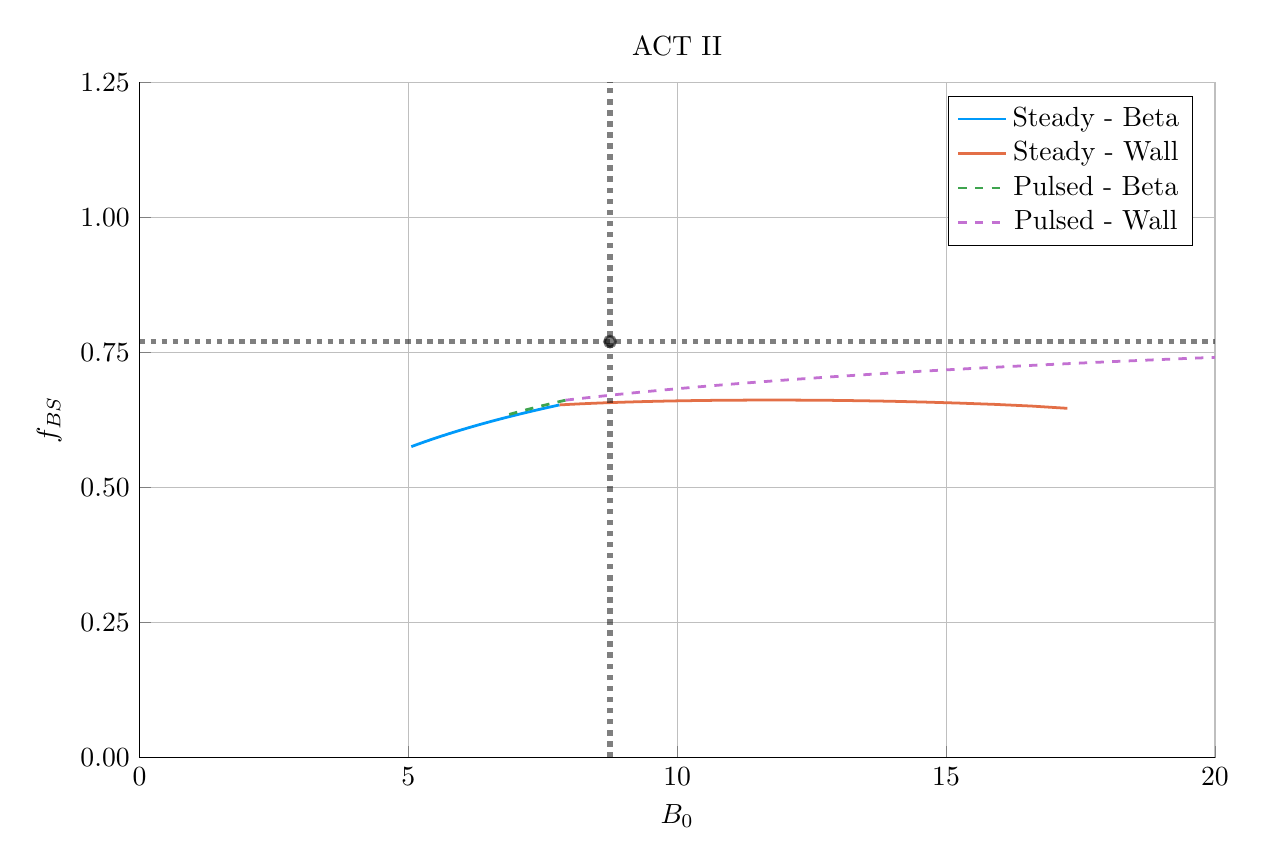
\begin{tikzpicture}[]
\begin{axis}[height = {101.6mm}, ylabel = {${f}_{BS}$}, title = {ACT II}, xmin = {0.0}, xmax = {20.0}, ymax = {1.25}, xlabel = {${B}_{0}$}, {unbounded coords=jump, scaled x ticks = false, xticklabel style={rotate = 0}, xmajorgrids = true, xtick = {0.0,5.0,10.0,15.0,20.0}, xticklabels = {0,5,10,15,20}, xtick align = inside, axis lines* = left, scaled y ticks = false, yticklabel style={rotate = 0}, ymajorgrids = true, ytick = {0.0,0.25,0.5,0.75,1.0,1.25}, yticklabels = {0.00,0.25,0.50,0.75,1.00,1.25}, ytick align = inside, axis lines* = left,     xshift = 0.0mm,
    yshift = 0.0mm,
    axis background/.style={fill={rgb,1:red,1.00000000;green,1.00000000;blue,1.00000000}}
, colorbar style={title=}}, ymin = {0.0}, width = {152.4mm}]\addplot+ [color = {rgb,1:red,0.00000000;green,0.60560316;blue,0.97868012},
draw opacity=1.0,
line width=1,
solid,mark = none,
mark size = 2.0,
mark options = {
    color = {rgb,1:red,0.00000000;green,0.00000000;blue,0.00000000}, draw opacity = 1.0,
    fill = {rgb,1:red,0.00000000;green,0.60560316;blue,0.97868012}, fill opacity = 1.0,
    line width = 1,
    rotate = 0,
    solid
}]coordinates {
(7.810935944285959, 0.6527702553932885)
(7.57736049850867, 0.647658545231261)
(7.354864292609041, 0.6425898820089996)
(7.145167234136329, 0.6376362714122338)
(6.9473303865083675, 0.632795343779806)
(6.760499508614096, 0.6280646919938583)
(6.583897990324067, 0.6234419458071817)
(6.416817229618043, 0.6189247365862985)
(6.258609820663305, 0.6145107131379413)
(6.108683264880386, 0.6101975467147034)
(5.966494431410919, 0.6059829352770211)
(5.831544666176381, 0.6018646071075806)
(5.703375459679132, 0.5978403237906162)
(5.581564609582325, 0.5939078827824683)
(5.465722802994068, 0.5900651194239572)
(5.355490573482678, 0.586309908593238)
(5.25053558682053, 0.5826401660556659)
(5.1505502068221745, 0.5790538493874968)
(5.0552493196883175, 0.5755489587457903)
};
\addlegendentry{Steady - Beta}
\addplot+ [color = {rgb,1:red,0.88887350;green,0.43564919;blue,0.27812294},
draw opacity=1.0,
line width=1,
solid,mark = none,
mark size = 2.0,
mark options = {
    color = {rgb,1:red,0.00000000;green,0.00000000;blue,0.00000000}, draw opacity = 1.0,
    fill = {rgb,1:red,0.88887350;green,0.43564919;blue,0.27812294}, fill opacity = 1.0,
    line width = 1,
    rotate = 0,
    solid
}]coordinates {
(17.25550839059296, 0.64644451726662)
(16.594334962335296, 0.6506097756344024)
(15.9071755430688, 0.6537415683998609)
(15.233983138507648, 0.6561541517880343)
(14.594239858921854, 0.6580477545565532)
(13.989673082630297, 0.6594991295949557)
(13.414782495717416, 0.6605221116367197)
(12.872659546281994, 0.6611976322308866)
(12.364365715508608, 0.6615901501928093)
(11.889507953196574, 0.661749881341293)
(11.44685939646348, 0.6617165976896415)
(11.034739998180656, 0.6615222104277009)
(10.651252523287319, 0.6611925961300233)
(10.294428800132035, 0.6607489265305431)
(9.962319203963213, 0.6602086590354735)
(9.653045819449929, 0.6595862878712827)
(9.364832254395445, 0.6588939220308313)
(9.096018465506306, 0.6581417353393015)
(8.844373144802077, 0.6573292662805607)
(8.61055754360846, 0.6564909703008925)
(8.391192178573277, 0.655605902097537)
(8.18577947665566, 0.654688439250136)
(7.99323348423048, 0.653743181184457)
(7.812301489248497, 0.6527702553932886)
};
\addlegendentry{Steady - Wall}
\addplot+ [color = {rgb,1:red,0.24222430;green,0.64327509;blue,0.30444865},
draw opacity=1.0,
line width=1,
dashed,mark = none,
mark size = 2.0,
mark options = {
    color = {rgb,1:red,0.00000000;green,0.00000000;blue,0.00000000}, draw opacity = 1.0,
    fill = {rgb,1:red,0.24222430;green,0.64327509;blue,0.30444865}, fill opacity = 1.0,
    line width = 1,
    rotate = 0,
    solid
}]coordinates {
(7.923668284887995, 0.661510566114555)
(7.923668284887995, 0.6615105661145547)
(7.836759696043437, 0.6595216595121864)
(7.6662731560983355, 0.6555277670578231)
(7.50499428233835, 0.651631171116251)
(7.35232773269976, 0.6478299013667072)
(7.207727224738343, 0.6441219962752663)
(7.070690693175276, 0.6405055068727987)
(6.940756001029682, 0.6369784999966126)
(6.817497143644154, 0.6335390612449313)
};
\addlegendentry{Pulsed - Beta}
\addplot+ [color = {rgb,1:red,0.76444018;green,0.44411178;blue,0.82429754},
draw opacity=1.0,
line width=1,
dashed,mark = none,
mark size = 2.0,
mark options = {
    color = {rgb,1:red,0.00000000;green,0.00000000;blue,0.00000000}, draw opacity = 1.0,
    fill = {rgb,1:red,0.76444018;green,0.44411178;blue,0.82429754}, fill opacity = 1.0,
    line width = 1,
    rotate = 0,
    solid
}]coordinates {
(22.56106430311702, 0.750175662985688)
(20.85607192394036, 0.7441240116987325)
(19.335265246056654, 0.7381977892183877)
(17.974121547130903, 0.7323964975504869)
(16.751976718553127, 0.7267194065154795)
(15.651329744019142, 0.7211655842793718)
(14.65728744097675, 0.7157339224745852)
(13.757118584462601, 0.7104231590647407)
(12.939893642194303, 0.7052318991619849)
(12.196191964860315, 0.7001586338992175)
(11.517862472405039, 0.6952017574713956)
(10.897827027335556, 0.6903595824666324)
(10.329918077124672, 0.6856303536550991)
(9.808743940706389, 0.6810122602790344)
(9.329576544487265, 0.6765034470860328)
(8.888257451278507, 0.6721020241407819)
(8.481118883411932, 0.6678060755607708)
(8.10491708701527, 0.6636136672742595)
(7.923668284887995, 0.661510566114555)
(7.923668284887995, 0.6615105661145547)
};
\addlegendentry{Pulsed - Wall}
\addplot+ [color = {rgb,1:red,0.00000000;green,0.00000000;blue,0.00000000},
draw opacity=0.5,
line width=2,
dotted,mark = none,
mark size = 2.0,
mark options = {
    color = {rgb,1:red,0.00000000;green,0.00000000;blue,0.00000000}, draw opacity = 0.5,
    fill = {rgb,1:red,0.00000000;green,0.00000000;blue,0.00000000}, fill opacity = 0.5,
    line width = 1,
    rotate = 0,
    solid
},forget plot]coordinates {
(0.0, 0.77)
(20.0, 0.77)
};
\addplot+ [color = {rgb,1:red,0.00000000;green,0.00000000;blue,0.00000000},
draw opacity=0.5,
line width=2,
dotted,mark = none,
mark size = 2.0,
mark options = {
    color = {rgb,1:red,0.00000000;green,0.00000000;blue,0.00000000}, draw opacity = 0.5,
    fill = {rgb,1:red,0.00000000;green,0.00000000;blue,0.00000000}, fill opacity = 0.5,
    line width = 1,
    rotate = 0,
    solid
},forget plot]coordinates {
(8.75, 0.0)
(8.75, 1.25)
};
\addplot+[draw=none, color = {rgb,1:red,0.00000000;green,0.00000000;blue,0.00000000},
draw opacity=0.5,
line width=0,
solid,mark = *,
mark size = 2.0,
mark options = {
    color = {rgb,1:red,0.00000000;green,0.00000000;blue,0.00000000}, draw opacity = 0.5,
    fill = {rgb,1:red,0.00000000;green,0.00000000;blue,0.00000000}, fill opacity = 0.5,
    line width = 1,
    rotate = 0,
    solid
},forget plot] coordinates {
(8.75, 0.77)
};
\end{axis}

\end{tikzpicture}

    \end{adjustbox}
        \caption{ACT II}
    \end{subfigure}
    \hfill \hfill ~\\ ~\\ ~\\ ~\\
  \caption[]{Magnet Scan: $f_{BS}$ vs $B_0$} ~\\
\end{figure*}


\clearpage

\newpage

\subsection*{ Magnetic Energy -- $W_M$ }
  \label{subsection:scan_W_M}

\begin{figure*}[h!]
    \centering
    \hfill
    \begin{subfigure}[t]{0.45\textwidth}
        \centering
    \begin{adjustbox}{width=\textwidth}
      \Large
      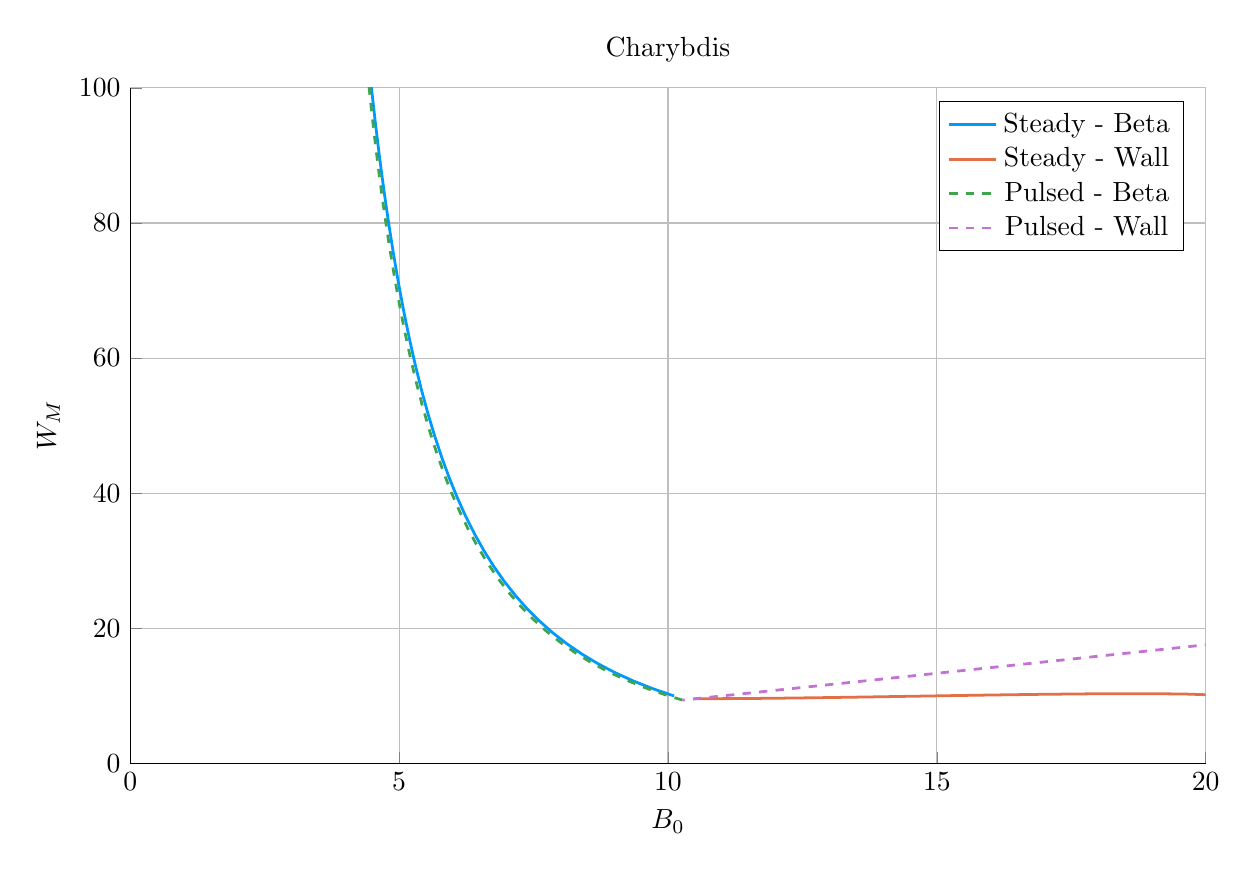
\begin{tikzpicture}[]
\begin{axis}[height = {101.6mm}, ylabel = {${W}_{M}$}, title = {Charybdis}, xmin = {0.0}, xmax = {20.0}, ymax = {100.0}, xlabel = {${B}_{0}$}, {unbounded coords=jump, scaled x ticks = false, xticklabel style={rotate = 0}, xmajorgrids = true, xtick = {0.0,5.0,10.0,15.0,20.0}, xticklabels = {0,5,10,15,20}, xtick align = inside, axis lines* = left, scaled y ticks = false, yticklabel style={rotate = 0}, ymajorgrids = true, ytick = {0.0,20.0,40.0,60.0,80.0,100.0}, yticklabels = {0,20,40,60,80,100}, ytick align = inside, axis lines* = left,     xshift = 0.0mm,
    yshift = 0.0mm,
    axis background/.style={fill={rgb,1:red,1.00000000;green,1.00000000;blue,1.00000000}}
, colorbar style={title=}}, ymin = {0.0}, width = {152.4mm}]\addplot+ [color = {rgb,1:red,0.00000000;green,0.60560316;blue,0.97868012},
draw opacity=1.0,
line width=1,
solid,mark = none,
mark size = 2.0,
mark options = {
    color = {rgb,1:red,0.00000000;green,0.00000000;blue,0.00000000}, draw opacity = 1.0,
    fill = {rgb,1:red,0.00000000;green,0.60560316;blue,0.97868012}, fill opacity = 1.0,
    line width = 1,
    rotate = 0,
    solid
}]coordinates {
(10.112818033153026, 9.976578426492665)
(9.722156888543116, 11.039660466609112)
(9.357875603858393, 12.186046944292867)
(9.017653755630063, 13.41983183975602)
(8.6995124437054, 14.745015003302626)
(8.401566530516865, 16.16580885971097)
(8.122163706328223, 17.68640812228457)
(7.859819415455661, 19.311037272036963)
(7.613196557650265, 21.043944124847812)
(7.381088038653343, 22.88939338318679)
(7.162401716104116, 24.851660192929742)
(6.956147367527331, 26.935023724984866)
(6.761425371986388, 29.143760800574988)
(6.577416849463348, 31.48213957811243)
(6.403375044688587, 33.954413318661445)
(6.2386177769852695, 36.564814245995436)
(6.0825208065966905, 39.317547514154995)
(5.934511989185341, 42.21678530918363)
(5.794066116682695, 45.26666106650895)
(5.660700347012839, 48.47126385772276)
(5.533970150598111, 51.83463292659603)
(5.413465705416883, 55.36075239855555)
(5.298808685607224, 59.053546158789416)
(5.189649392059402, 62.916872936825555)
(5.085664187259174, 66.95452156427906)
(4.986553195072601, 71.17020644245522)
(4.892038235455667, 75.56756321268114)
(4.801860966679364, 80.15014463577118)
(4.7157812114040425, 84.92141668413309)
(4.633575445956479, 89.88475484920548)
(4.5550354347559185, 95.04344066616578)
(4.479966994069385, 100.40065845709658)
(4.408188871204256, 105.95949229312403)
(4.33953172691477, 111.722923175371)
(4.273837210246432, 117.69382643395397)
(4.210957116299974, 123.87496934366592)
(4.15075261849161, 130.26900895445985)
(4.0930935678432965, 136.87849013432438)
(4.037857852672517, 143.70584382168556)
(3.9849308127842145, 150.75338548402638)
(3.9342047029103653, 158.0233137790392)
(3.8855782007091695, 165.51770941424607)
(3.838955955133626, 173.2385342006938)
(3.7942481714200484, 181.18763029604904)
(3.7513702293348077, 189.3667196321631)
(3.710242331663442, 197.7774035219001)
(3.6707891802306123, 206.42116243987095)
(3.6329396770109583, 215.29935597152118)
(3.5966266481325166, 224.4132229248458)
(3.5617865887889004, 233.7638815989369)
(3.5283594272686503, 243.35233020340158)
(3.496288306480746, 253.17944742270524)
(3.465519381509793, 263.2459931193115)
(3.4360016318699595, 273.55260916960026)
(3.4076866872513096, 284.0998204264205)
(3.380528665662031, 294.8880358021726)
(3.3544840229690007, 305.91754946638855)
(3.3295114129297314, 317.1885421516888)
(3.3055715568879336, 328.70108256218947)
(3.2826271223788512, 340.455128878375)
(3.260642607548369, 352.45053061276974)
(3.239584247604666, 364.68702898947515)
(3.2194198921826622, 377.164261305329)
(3.2001189373344725, 389.8817601613681)
(3.181652227422265, 402.838956664921)
(3.163991977015565, 416.0351821334508)
(3.1471116955378684, 429.46967011616175)
(3.130986116696265, 443.1415584680792)
(3.115591132350856, 457.0498914716555)
(3.1009037305081053, 471.193622001098)
(3.0869019371473265, 485.5716137247627)
(3.0735647616124355, 500.18264334105356)
(3.0608721453218655, 515.0254028435138)
};
\addlegendentry{Steady - Beta}
\addplot+ [color = {rgb,1:red,0.88887350;green,0.43564919;blue,0.27812294},
draw opacity=1.0,
line width=1,
solid,mark = none,
mark size = 2.0,
mark options = {
    color = {rgb,1:red,0.00000000;green,0.00000000;blue,0.00000000}, draw opacity = 1.0,
    fill = {rgb,1:red,0.88887350;green,0.43564919;blue,0.27812294}, fill opacity = 1.0,
    line width = 1,
    rotate = 0,
    solid
}]coordinates {
(20.758867641064707, 9.553910503525564)
(20.346250098246923, 10.073407723171604)
(19.57104597888471, 10.271705003276914)
(18.681781921115476, 10.317535819458373)
(17.775790175980152, 10.285009745556987)
(16.896654716492492, 10.212829314419727)
(16.063927450323227, 10.12269815340002)
(15.285557510665852, 10.027430597336357)
(14.563500533069154, 9.934731969591997)
(13.896568848875791, 9.84922114882318)
(13.281970890030232, 9.773597384382443)
(12.716170469467318, 9.709346960001346)
(12.195372283741088, 9.657185133921969)
(11.715794270833433, 9.617338533567926)
(11.273815669498969, 9.589728187292506)
(10.866051794088186, 9.574089192034752)
(10.489365023931143, 9.570018344615757)
};
\addlegendentry{Steady - Wall}
\addplot+ [color = {rgb,1:red,0.24222430;green,0.64327509;blue,0.30444865},
draw opacity=1.0,
line width=1,
dashed,mark = none,
mark size = 2.0,
mark options = {
    color = {rgb,1:red,0.00000000;green,0.00000000;blue,0.00000000}, draw opacity = 1.0,
    fill = {rgb,1:red,0.24222430;green,0.64327509;blue,0.30444865}, fill opacity = 1.0,
    line width = 1,
    rotate = 0,
    solid
}]coordinates {
(10.26788634689966, 9.364392881177613)
(9.953967652326213, 10.13578964133185)
(9.567926244368271, 11.217614800887029)
(9.207974394987358, 12.384429681901585)
(8.871841888699304, 13.640391534011185)
(8.557505525932248, 14.989700107716784)
(8.263156925406376, 16.436589536002487)
(7.9871752024348766, 17.985320029331078)
(7.728103682045175, 19.640169429400935)
(7.484629973620137, 21.4054246549726)
(7.255568856523303, 23.285373077366984)
(7.039847526735421, 25.284293862600023)
(6.836492834698909, 27.406449316799772)
(6.644620209081183, 29.656076270965524)
(6.463424013335149, 32.0373775402961)
(6.2921691243175495, 34.55451349225141)
(6.13018355681404, 37.211593756221255)
(5.97685198655569, 40.01266910359221)
(5.831610044919842, 42.96172354330629)
(5.693939286027163, 46.06266662246393)
(5.563362729090489, 49.31932600850176)
(5.439440906144732, 52.735440338904496)
(5.321768347746793, 56.31465237725817)
(5.209970453003084, 60.06050247784679)
(5.103700692769835, 63.97642241235568)
(5.002638109938164, 68.06572952340464)
(4.906485077678376, 72.33162125452287)
(4.814965286571576, 76.77717005097541)
(4.727821933804548, 81.40531864120021)
(4.644816091323922, 86.21887570379593)
(4.565725232806084, 91.22051192272993)
(4.490341901840154, 96.41275643132924)
(4.418472505906755, 101.79799364357935)
(4.349936222622964, 107.37846046932441)
(4.284564006352339, 113.15624390821931)
(4.222197684694192, 119.13327901560542)
(4.162689135592264, 125.31134723201787)
(4.105899536872315, 131.6920750666788)
(4.051698680949713, 138.27693312415383)
(3.9999643482627323, 145.06723546232206)
(3.9505817337017928, 152.06413926890778)
(3.903442920928527, 159.26864484317642)
(3.858446400032002, 166.6815958687351)
(3.8154966244515616, 174.30367996301612)
(3.7745036035252744, 182.13542948869875)
(3.7353825273991994, 190.17722261219166)
(3.6980534213689746, 198.42928459421515)
(3.6624408270205375, 206.89168929763431)
(3.62847350780097, 215.56436089783668)
(3.5960841768845415, 224.4470757812065)
(3.565209245407392, 233.5394646176475)
(3.5357885893311605, 242.8410145934057)
(3.5077653333614305, 252.35107179105523)
(3.4810856504959875, 262.06884370391384)
(3.4556985759109375, 271.9934018728071)
(3.4315558340122845, 282.1236846336368)
(3.408611677587535, 292.45849996487783)
(3.3868227380888998, 302.9965284247168)
(3.36614788616562, 313.7363261682407)
(3.3465481016421226, 324.67632803565135)
(3.327986352208224, 335.81485070321526)
(3.3104274769652595, 347.15009622338533)
(3.2938380965241474, 358.6801536076612)
(3.278186482171801, 370.4030054636531)
(3.263442495132517, 382.31652798375063)
(3.2495774839156075, 394.4184959765958)
(3.236564206241785, 406.7065859184474)
(3.224376752844934, 419.1783793593078)
(3.212990475972638, 431.83136634561106)
(3.2023819222517877, 444.6629488558077)
(3.192528769611062, 457.6704442456245)
(3.1834097679780142, 470.85108870001955)
(3.1750046834890777, 484.2020406892131)
(3.1672942459724482, 497.7203844263853)
};
\addlegendentry{Pulsed - Beta}
\addplot+ [color = {rgb,1:red,0.76444018;green,0.44411178;blue,0.82429754},
draw opacity=1.0,
line width=1,
dashed,mark = none,
mark size = 2.0,
mark options = {
    color = {rgb,1:red,0.00000000;green,0.00000000;blue,0.00000000}, draw opacity = 1.0,
    fill = {rgb,1:red,0.76444018;green,0.44411178;blue,0.82429754}, fill opacity = 1.0,
    line width = 1,
    rotate = 0,
    solid
}]coordinates {
(48.990476413653056, 42.85867778392443)
(42.83950920694117, 37.351649161331494)
(37.687790427214495, 32.79775226816225)
(33.33937742845888, 28.994864760672673)
(29.64296398154308, 25.790954482861412)
(26.48039367255613, 23.070054107565483)
(23.758442882319894, 20.74256902268996)
(21.402860298405816, 18.73846610398629)
(19.353987387634486, 17.00241252520485)
(17.563502020363714, 15.49025654204321)
(15.991970371213752, 14.166446024582525)
(14.606987499719377, 13.002111598152931)
(13.381751501116137, 11.973627056777696)
(12.293960329570087, 11.061516731361111)
(11.32495111804522, 10.249617976796117)
(10.459023415380802, 9.524433264185083)
(10.26788634689966, 9.364392881177613)
};
\addlegendentry{Pulsed - Wall}
\end{axis}

\end{tikzpicture}

    \end{adjustbox}
        \caption{Charybdis}
    \end{subfigure}
    \hfill
    \begin{subfigure}[t]{0.45\textwidth}
        \centering
    \begin{adjustbox}{width=\textwidth}
      \Large
      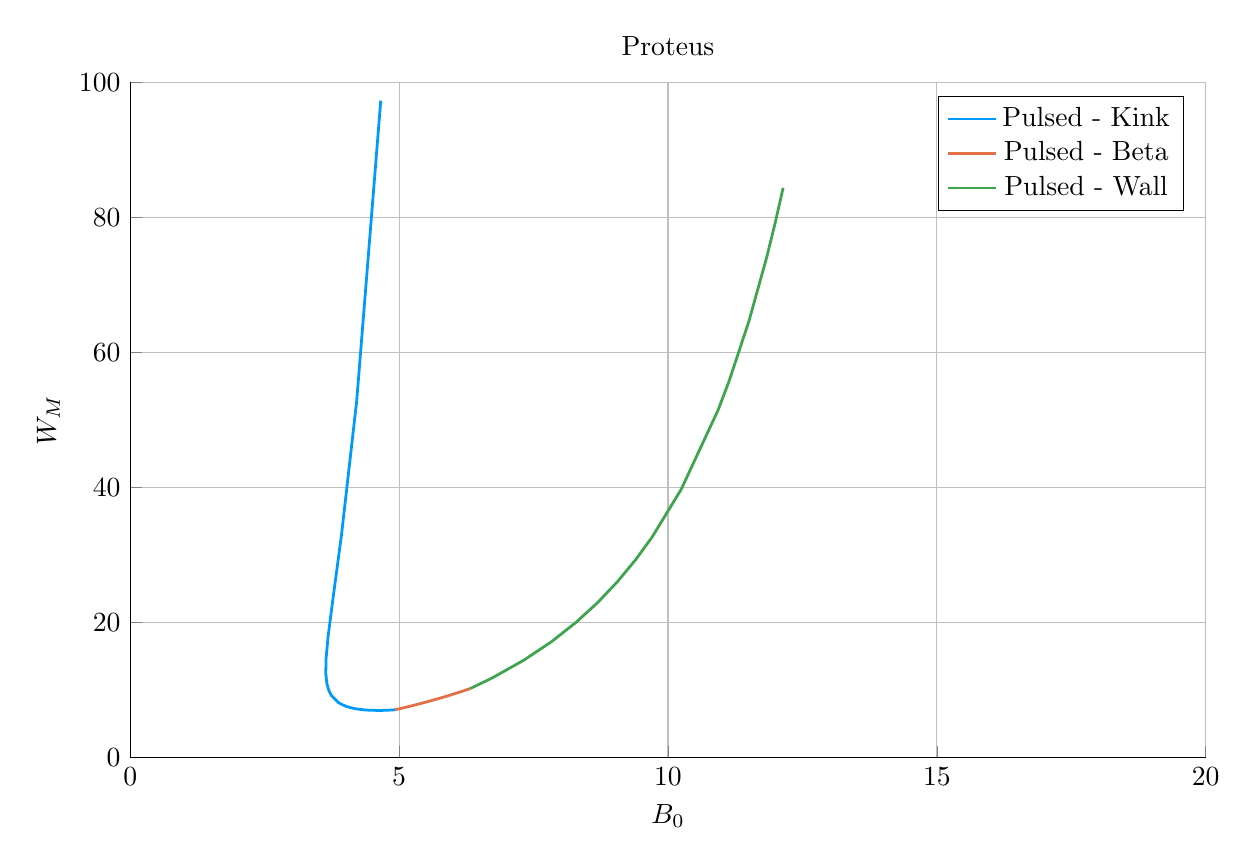
\begin{tikzpicture}[]
\begin{axis}[height = {101.6mm}, ylabel = {${W}_{M}$}, title = {Proteus}, xmin = {0.0}, xmax = {20.0}, ymax = {100.0}, xlabel = {${B}_{0}$}, {unbounded coords=jump, scaled x ticks = false, xticklabel style={rotate = 0}, xmajorgrids = true, xtick = {0.0,5.0,10.0,15.0,20.0}, xticklabels = {0,5,10,15,20}, xtick align = inside, axis lines* = left, scaled y ticks = false, yticklabel style={rotate = 0}, ymajorgrids = true, ytick = {0.0,20.0,40.0,60.0,80.0,100.0}, yticklabels = {0,20,40,60,80,100}, ytick align = inside, axis lines* = left,     xshift = 0.0mm,
    yshift = 0.0mm,
    axis background/.style={fill={rgb,1:red,1.00000000;green,1.00000000;blue,1.00000000}}
, colorbar style={title=}}, ymin = {0.0}, width = {152.4mm}]\addplot+ [color = {rgb,1:red,0.00000000;green,0.60560316;blue,0.97868012},
draw opacity=1.0,
line width=1,
solid,mark = none,
mark size = 2.0,
mark options = {
    color = {rgb,1:red,0.00000000;green,0.00000000;blue,0.00000000}, draw opacity = 1.0,
    fill = {rgb,1:red,0.00000000;green,0.60560316;blue,0.97868012}, fill opacity = 1.0,
    line width = 1,
    rotate = 0,
    solid
}]coordinates {
(4.658732060637907, 97.28232425378617)
(4.211109766361548, 52.81528522659042)
(3.9293920326356777, 33.045940900779435)
(3.7651903683456465, 23.247661382566328)
(3.6776039543745567, 17.827034690374397)
(3.6402437753208394, 14.548456710153735)
(3.6366994671255806, 12.424185075208992)
(3.656621534643579, 10.973706805818463)
(3.693300156736026, 9.943115007776825)
(3.7422515017241134, 9.18863958559583)
(3.865532743079537, 8.195040941316238)
(3.936096932264377, 7.866037710488523)
(4.010907188015084, 7.612872940496481)
(4.089072356933184, 7.418652478460303)
(4.169903401491354, 7.271257368183174)
(4.252857906625248, 7.16179941021134)
(4.337501757261618, 7.083633084260422)
(4.42348218754058, 7.031705491759868)
(4.5983381267510195, 6.991823293679325)
(4.686766232902671, 6.998413622496496)
(4.775618142770625, 7.019967223555443)
(4.864743502376605, 7.054937735216179)
(4.927312314219091, 7.086769144908002)
};
\addlegendentry{Pulsed - Kink}
\addplot+ [color = {rgb,1:red,0.88887350;green,0.43564919;blue,0.27812294},
draw opacity=1.0,
line width=1,
solid,mark = none,
mark size = 2.0,
mark options = {
    color = {rgb,1:red,0.00000000;green,0.00000000;blue,0.00000000}, draw opacity = 1.0,
    fill = {rgb,1:red,0.88887350;green,0.43564919;blue,0.27812294}, fill opacity = 1.0,
    line width = 1,
    rotate = 0,
    solid
}]coordinates {
(4.927312314219091, 7.086769144908002)
(4.984545814413324, 7.193516773221651)
(5.17452482724068, 7.558989804600146)
(5.362091669637646, 7.937858802904825)
(5.54700293215903, 8.330611438237515)
(5.729042482638278, 8.737734587814298)
(5.908022832274664, 9.159710709615348)
(6.083785777786694, 9.597014749238335)
(6.256202341425288, 10.050111620812826)
(6.324169421042356, 10.235766195929495)
};
\addlegendentry{Pulsed - Beta}
\addplot+ [color = {rgb,1:red,0.24222430;green,0.64327509;blue,0.30444865},
draw opacity=1.0,
line width=1,
solid,mark = none,
mark size = 2.0,
mark options = {
    color = {rgb,1:red,0.00000000;green,0.00000000;blue,0.00000000}, draw opacity = 1.0,
    fill = {rgb,1:red,0.24222430;green,0.64327509;blue,0.30444865}, fill opacity = 1.0,
    line width = 1,
    rotate = 0,
    solid
}]coordinates {
(6.324169421042356, 10.235766195929495)
(6.727338549778396, 11.783493156592025)
(7.320469048424473, 14.433662866898274)
(7.835746509376305, 17.179550950209588)
(8.290245520072391, 20.029490714669382)
(8.696162676727877, 22.99147222981706)
(9.0624397222742, 26.07266302814804)
(9.395798186463841, 29.27939084761122)
(9.701405747258567, 32.61725020270231)
(10.244760202900984, 39.70580850721064)
(10.930275827723788, 51.43239308745394)
(11.131878682735255, 55.64715526987581)
(11.50278450645086, 64.55415559202683)
(11.83715172742864, 74.11630708302644)
(11.992609772603878, 79.14953842129572)
(12.141110720831467, 84.35411724014395)
};
\addlegendentry{Pulsed - Wall}
\end{axis}

\end{tikzpicture}

    \end{adjustbox}
        \caption{Proteus}
    \end{subfigure}
    \hfill \hfill ~\\ ~\\ ~\\ ~\\
    \hfill
    \begin{subfigure}[t]{0.45\textwidth}
        \centering
    \begin{adjustbox}{width=\textwidth}
      \Large
      \begin{tikzpicture}[]
\begin{axis}[height = {101.6mm}, ylabel = {${W}_{M}$}, title = {ARC}, xmin = {0.0}, xmax = {20.0}, ymax = {100.0}, xlabel = {${B}_{0}$}, {unbounded coords=jump, scaled x ticks = false, xticklabel style={rotate = 0}, xmajorgrids = true, xtick = {0.0,5.0,10.0,15.0,20.0}, xticklabels = {0,5,10,15,20}, xtick align = inside, axis lines* = left, scaled y ticks = false, yticklabel style={rotate = 0}, ymajorgrids = true, ytick = {0.0,20.0,40.0,60.0,80.0,100.0}, yticklabels = {0,20,40,60,80,100}, ytick align = inside, axis lines* = left,     xshift = 0.0mm,
    yshift = 0.0mm,
    axis background/.style={fill={rgb,1:red,1.00000000;green,1.00000000;blue,1.00000000}}
, colorbar style={title=}}, ymin = {0.0}, width = {152.4mm}]\addplot+ [color = {rgb,1:red,0.00000000;green,0.60560316;blue,0.97868012},
draw opacity=1.0,
line width=1,
solid,mark = none,
mark size = 2.0,
mark options = {
    color = {rgb,1:red,0.00000000;green,0.00000000;blue,0.00000000}, draw opacity = 1.0,
    fill = {rgb,1:red,0.00000000;green,0.60560316;blue,0.97868012}, fill opacity = 1.0,
    line width = 1,
    rotate = 0,
    solid
}]coordinates {
(9.701206080853105, 5.427771381863723)
(9.162315904693079, 6.0987738692375775)
(8.664301107137337, 6.83618423325786)
(8.203576462497304, 7.644721043949607)
(7.776718537485166, 8.529472293380365)
(7.380720231870917, 9.495691334286995)
(7.012886014999712, 10.548836597070189)
(6.670795005901889, 11.69456941984695)
(6.352268997292712, 12.938751267320981)
(6.055344682097163, 14.287440342985972)
(5.778249464564785, 15.746887601937072)
(5.519380338856715, 17.323532174227967)
(5.2772854007125325, 19.023996211252612)
(5.050647625972996, 20.855079170039314)
(4.838270606140816, 22.823751552623147)
(4.639065978019038, 24.93714811977536)
(4.4520423235376105, 27.20256060033298)
(4.276295348572609, 29.62742991917287)
(4.110999177018484, 32.2193379684975)
(3.9553986195015125, 34.985998948560784)
(3.8088022956698633, 37.935250305246754)
(3.6705765055641186, 41.07504329302362)
(3.54013975965751, 44.41343319273597)
(3.4169578891619192, 47.95856921447045)
(3.30053966845824, 51.71868411632614)
(3.1904328903033052, 55.70208357037785)
(3.086220842019516, 59.91713530738777)
(2.9875191373772063, 64.37225807197102)
(2.8939728644914635, 69.07591041990094)
(2.8052540149097247, 74.03657938910177)
(2.7210591632720242, 79.26276907558959)
(2.6411073705789065, 84.76298914523422)
(2.565138287279709, 90.54574331169599)
(2.492910435164382, 96.6195178102755)
(2.4241996494611984, 102.99276989670221)
(2.3587976646588236, 109.67391639907238)
(2.296510829425685, 116.67132235029027)
(2.237158937627476, 123.99328972736632)
(2.180574163874242, 131.6480463229597)
(2.126600093288366, 139.64373477342252)
(2.075090836295778, 147.9884017665293)
(2.0259102202234582, 156.68998745087276)
(1.978931050353818, 165.75631506772302)
(1.9340344338545452, 175.19508082494886)
(1.8911091606836798, 185.01384403129848)
(1.8500511361739687, 195.2200175081485)
(1.8107628605384507, 205.8208582945099)
(1.773152951016952, 216.8234586598709)
(1.7371357028100902, 228.23473743812232)
(1.7026306853269466, 240.06143169464215)
(1.6695623706125668, 252.31008873731273)
(1.6378597911249178, 264.9870584810501)
(1.607456224302725, 278.0984861742324)
(1.5782889016090462, 291.65030549419623)
(1.5502987399539199, 305.6482320178956)
(1.5234300935954943, 320.09775707261554)
(1.4976305247952577, 335.0041419706059)
(1.4728505916614916, 350.3724126304409)
(1.4490436517578602, 366.20735458689427)
(1.4261656801829077, 382.51350839009586)
};
\addlegendentry{Steady - Beta}
\addplot+ [color = {rgb,1:red,0.88887350;green,0.43564919;blue,0.27812294},
draw opacity=1.0,
line width=1,
solid,mark = none,
mark size = 2.0,
mark options = {
    color = {rgb,1:red,0.00000000;green,0.00000000;blue,0.00000000}, draw opacity = 1.0,
    fill = {rgb,1:red,0.88887350;green,0.43564919;blue,0.27812294}, fill opacity = 1.0,
    line width = 1,
    rotate = 0,
    solid
}]coordinates {
(19.394007482712425, 4.921510212098785)
(18.932196567189358, 5.148330413697917)
(18.296989378345195, 5.283475689295352)
(17.587029315408756, 5.360366139863426)
(16.847882407994106, 5.395581006581063)
(16.111374502564406, 5.403150640145799)
(15.396027314547156, 5.392849464432363)
(14.710952688793137, 5.370784448778517)
(14.06168447794857, 5.3418459364491655)
(13.450465418483889, 5.309433549930485)
(12.877644538645335, 5.275983644700812)
(12.342394470642008, 5.243229495965154)
(11.843182246608265, 5.212389363078008)
(11.376441269625893, 5.183073560195945)
(10.944966372727551, 5.159537018545776)
(10.541663878705513, 5.138450718137239)
(10.165908182236457, 5.121168207292785)
};
\addlegendentry{Steady - Wall}
\addplot+ [color = {rgb,1:red,0.24222430;green,0.64327509;blue,0.30444865},
draw opacity=1.0,
line width=1,
dashed,mark = none,
mark size = 2.0,
mark options = {
    color = {rgb,1:red,0.00000000;green,0.00000000;blue,0.00000000}, draw opacity = 1.0,
    fill = {rgb,1:red,0.24222430;green,0.64327509;blue,0.30444865}, fill opacity = 1.0,
    line width = 1,
    rotate = 0,
    solid
}]coordinates {
(9.980483622051658, 4.993794215649894)
(9.392786903460065, 5.60599631146957)
(8.79273598103983, 6.355120060665557)
(8.23820290909994, 7.1897669035785094)
(7.725182218401588, 8.118132601340655)
(7.250078106370205, 9.149046993109769)
(6.80965553466646, 10.292009748479334)
(6.400998063035608, 11.55722715701422)
(6.0214713600430425, 12.955649976143105)
(5.668691517461799, 14.499012388644925)
(5.340497445229901, 16.199872163398506)
(5.034926745580058, 18.071652171370758)
(4.750194564008521, 20.128683487292683)
(4.484674995755211, 22.386250411429753)
(4.236884692979903, 24.860637881923484)
(4.00546837264544, 27.569181924655858)
(3.7891859704718387, 30.530324014913937)
(3.5869012239550364, 33.7636705166201)
(3.3975714987448393, 37.290058737638056)
(3.2202386987489797, 41.13163161601345)
(3.0540211220494466, 45.311923661534536)
(2.8981061427709687, 49.85596155953255)
(2.7517436139566023, 54.79038385397311)
(2.6142398986781377, 60.14358544064732)
(2.4849524463010138, 65.94589432656355)
(2.363284838174807, 72.22979040403317)
(2.248682232019848, 79.03017907591492)
(2.140627136740878, 86.3847367932101)
(2.038635448877246, 94.33435144675408)
(1.9422526775794744, 102.92368889632095)
(1.8510502754751532, 112.20192899846954)
(1.7646219756564088, 122.22373237713917)
(1.6825800061969869, 133.0505263103484)
(1.6045510059627948, 144.7522403812059)
(1.53017138625397, 157.4096904134694)
(1.4590817483192686, 171.1179219178268)
(1.3909197311384796, 185.99101880909595)
(1.3253102336217724, 202.16923439023455)
(1.261851128383913, 219.82997049317157)
(1.20009089049112, 239.20548919331128)
(1.1394908096975784, 260.61322905720664)
};
\addlegendentry{Pulsed - Beta}
\addplot+ [color = {rgb,1:red,0.76444018;green,0.44411178;blue,0.82429754},
draw opacity=1.0,
line width=1,
dashed,mark = none,
mark size = 2.0,
mark options = {
    color = {rgb,1:red,0.00000000;green,0.00000000;blue,0.00000000}, draw opacity = 1.0,
    fill = {rgb,1:red,0.76444018;green,0.44411178;blue,0.82429754}, fill opacity = 1.0,
    line width = 1,
    rotate = 0,
    solid
}]coordinates {
(29.27715761652869, 17.891002682759158)
(25.4410619834368, 15.180151128834671)
(22.158819835998365, 12.906626963925868)
(19.342453256965573, 10.994997402629936)
(16.919364280634177, 9.383840103068328)
(14.829378672669455, 8.022920717873049)
(13.022412368922526, 6.870989960397289)
(11.456617692058645, 5.8940520461404295)
(10.096901921254785, 5.063994772567079)
(9.980483622051658, 4.993794215649894)
};
\addlegendentry{Pulsed - Wall}
\addplot+ [color = {rgb,1:red,0.00000000;green,0.00000000;blue,0.00000000},
draw opacity=0.5,
line width=2,
dotted,mark = none,
mark size = 2.0,
mark options = {
    color = {rgb,1:red,0.00000000;green,0.00000000;blue,0.00000000}, draw opacity = 0.5,
    fill = {rgb,1:red,0.00000000;green,0.00000000;blue,0.00000000}, fill opacity = 0.5,
    line width = 1,
    rotate = 0,
    solid
},forget plot]coordinates {
(0.0, NaN)
(20.0, NaN)
};
\addplot+ [color = {rgb,1:red,0.00000000;green,0.00000000;blue,0.00000000},
draw opacity=0.5,
line width=2,
dotted,mark = none,
mark size = 2.0,
mark options = {
    color = {rgb,1:red,0.00000000;green,0.00000000;blue,0.00000000}, draw opacity = 0.5,
    fill = {rgb,1:red,0.00000000;green,0.00000000;blue,0.00000000}, fill opacity = 0.5,
    line width = 1,
    rotate = 0,
    solid
},forget plot]coordinates {
(9.2, 0.0)
(9.2, 100.0)
};
\addplot+[draw=none, color = {rgb,1:red,0.00000000;green,0.00000000;blue,0.00000000},
draw opacity=0.5,
line width=0,
solid,mark = *,
mark size = 2.0,
mark options = {
    color = {rgb,1:red,0.00000000;green,0.00000000;blue,0.00000000}, draw opacity = 0.5,
    fill = {rgb,1:red,0.00000000;green,0.00000000;blue,0.00000000}, fill opacity = 0.5,
    line width = 1,
    rotate = 0,
    solid
},forget plot] coordinates {
(9.2, NaN)
};
\end{axis}

\end{tikzpicture}

    \end{adjustbox}
        \caption{ARC}
    \end{subfigure}
    \hfill
    \begin{subfigure}[t]{0.45\textwidth}
        \centering
    \begin{adjustbox}{width=\textwidth}
      \Large
      \begin{tikzpicture}[]
\begin{axis}[height = {101.6mm}, ylabel = {${W}_{M}$}, title = {Demo Pulsed}, xmin = {0.0}, xmax = {20.0}, ymax = {100.0}, xlabel = {${B}_{0}$}, {unbounded coords=jump, scaled x ticks = false, xticklabel style={rotate = 0}, xmajorgrids = true, xtick = {0.0,5.0,10.0,15.0,20.0}, xticklabels = {0,5,10,15,20}, xtick align = inside, axis lines* = left, scaled y ticks = false, yticklabel style={rotate = 0}, ymajorgrids = true, ytick = {0.0,20.0,40.0,60.0,80.0,100.0}, yticklabels = {0,20,40,60,80,100}, ytick align = inside, axis lines* = left,     xshift = 0.0mm,
    yshift = 0.0mm,
    axis background/.style={fill={rgb,1:red,1.00000000;green,1.00000000;blue,1.00000000}}
, colorbar style={title=}}, ymin = {0.0}, width = {152.4mm}]\addplot+ [color = {rgb,1:red,0.00000000;green,0.60560316;blue,0.97868012},
draw opacity=1.0,
line width=1,
solid,mark = none,
mark size = 2.0,
mark options = {
    color = {rgb,1:red,0.00000000;green,0.00000000;blue,0.00000000}, draw opacity = 1.0,
    fill = {rgb,1:red,0.00000000;green,0.60560316;blue,0.97868012}, fill opacity = 1.0,
    line width = 1,
    rotate = 0,
    solid
}]coordinates {
(4.327031075670194, 123.44373673332173)
(4.038214026054326, 79.76523284023226)
(3.8713719163129245, 58.108897430981536)
(3.7758613845615545, 45.733304605517155)
(3.7257856761317214, 37.95828264093558)
(3.7090473695925437, 29.04694896379975)
(3.727711597554826, 26.344517979953586)
(3.7586131667481433, 24.306117941226923)
(3.799052518631718, 22.733747168495924)
(3.901290136389271, 20.517766605492294)
(3.960577465316514, 19.728940193613518)
(4.0241209645210345, 19.090733790490855)
(4.0912717805663785, 18.572256162198553)
(4.161514602943343, 18.150497380470465)
(4.2344343960723005, 17.808002600991745)
(4.309692554546368, 17.531315861496644)
(4.450417240491067, 17.166473566094577)
};
\addlegendentry{Pulsed - Kink}
\addplot+ [color = {rgb,1:red,0.88887350;green,0.43564919;blue,0.27812294},
draw opacity=1.0,
line width=1,
solid,mark = none,
mark size = 2.0,
mark options = {
    color = {rgb,1:red,0.00000000;green,0.00000000;blue,0.00000000}, draw opacity = 1.0,
    fill = {rgb,1:red,0.88887350;green,0.43564919;blue,0.27812294}, fill opacity = 1.0,
    line width = 1,
    rotate = 0,
    solid
}]coordinates {
(4.450417240491067, 17.166473566094577)
(4.490148631384312, 17.305309015848636)
(4.692490181445514, 18.019389484737392)
(4.8960344619053355, 18.749800407200777)
(5.100651132702229, 19.496700146051747)
(5.306202822090688, 20.26030213940914)
(5.512545696627038, 21.04087102241869)
(5.719530043226767, 21.83871936060431)
(5.927000883375481, 22.654204785704835)
};
\addlegendentry{Pulsed - Beta}
\addplot+ [color = {rgb,1:red,0.24222430;green,0.64327509;blue,0.30444865},
draw opacity=1.0,
line width=1,
dashed,mark = none,
mark size = 2.0,
mark options = {
    color = {rgb,1:red,0.00000000;green,0.00000000;blue,0.00000000}, draw opacity = 1.0,
    fill = {rgb,1:red,0.24222430;green,0.64327509;blue,0.30444865}, fill opacity = 1.0,
    line width = 1,
    rotate = 0,
    solid
}]coordinates {
(3.4087424183072135, 76.02109466923234)
(2.977074181068944, 36.99469776498375)
(2.8592500074202523, 26.602664601337402)
(2.827199220063259, 21.660862067495565)
(2.8339789008667826, 18.765953821795108)
(2.862412302880871, 16.874407011263102)
(2.9044598258085443, 15.553537101768894)
(2.95577893007882, 14.590024878457532)
(3.0137895352525907, 13.865991589551562)
(3.076849710218805, 13.310773511983673)
(3.1438583711612704, 12.879335564625128)
(3.214045733980633, 12.54157019826116)
(3.2868548955983727, 12.276561049231674)
(3.361871149981842, 12.069311294803374)
(3.4387778750377818, 11.90878112839417)
(3.5173279629378453, 11.786660090388734)
};
\addlegendentry{Modified - Kink}
\addplot+ [color = {rgb,1:red,0.76444018;green,0.44411178;blue,0.82429754},
draw opacity=1.0,
line width=1,
dashed,mark = none,
mark size = 2.0,
mark options = {
    color = {rgb,1:red,0.00000000;green,0.00000000;blue,0.00000000}, draw opacity = 1.0,
    fill = {rgb,1:red,0.76444018;green,0.44411178;blue,0.82429754}, fill opacity = 1.0,
    line width = 1,
    rotate = 0,
    solid
}]coordinates {
(3.6607028750648505, 12.074397140834275)
(3.8574448036470477, 12.685277919648211)
(4.056375867871351, 13.310146449544076)
(4.257366397480293, 13.949057026240864)
(4.460279103534801, 14.602113733589642)
(4.664969389370631, 15.269467629207359)
(4.871285596007394, 15.951314711845848)
(5.07906923307514, 16.647894398080105)
(5.288155233306219, 17.359488308762714)
(5.498372259673351, 18.086419214151615)
(5.709543087166185, 18.82905002156669)
(5.921485076209294, 19.587782712469505)
(6.134010749367255, 20.363057156601585)
(6.346928478632384, 21.155349745799302)
(6.560043285872518, 21.965171804607706)
(6.773157754368795, 22.79306774804729)
(6.986073044284746, 23.639612971086876)
(7.198590001107076, 24.50541146426436)
};
\addlegendentry{Modified - Beta}
\addplot+ [color = {rgb,1:red,0.00000000;green,0.00000000;blue,0.00000000},
draw opacity=0.5,
line width=2,
dotted,mark = none,
mark size = 2.0,
mark options = {
    color = {rgb,1:red,0.00000000;green,0.00000000;blue,0.00000000}, draw opacity = 0.5,
    fill = {rgb,1:red,0.00000000;green,0.00000000;blue,0.00000000}, fill opacity = 0.5,
    line width = 1,
    rotate = 0,
    solid
},forget plot]coordinates {
(0.0, NaN)
(20.0, NaN)
};
\addplot+ [color = {rgb,1:red,0.00000000;green,0.00000000;blue,0.00000000},
draw opacity=0.5,
line width=2,
dotted,mark = none,
mark size = 2.0,
mark options = {
    color = {rgb,1:red,0.00000000;green,0.00000000;blue,0.00000000}, draw opacity = 0.5,
    fill = {rgb,1:red,0.00000000;green,0.00000000;blue,0.00000000}, fill opacity = 0.5,
    line width = 1,
    rotate = 0,
    solid
},forget plot]coordinates {
(5.667, 0.0)
(5.667, 100.0)
};
\addplot+[draw=none, color = {rgb,1:red,0.00000000;green,0.00000000;blue,0.00000000},
draw opacity=0.5,
line width=0,
solid,mark = *,
mark size = 2.0,
mark options = {
    color = {rgb,1:red,0.00000000;green,0.00000000;blue,0.00000000}, draw opacity = 0.5,
    fill = {rgb,1:red,0.00000000;green,0.00000000;blue,0.00000000}, fill opacity = 0.5,
    line width = 1,
    rotate = 0,
    solid
},forget plot] coordinates {
(5.667, NaN)
};
\end{axis}

\end{tikzpicture}

    \end{adjustbox}
        \caption{DEMO Pulsed}
    \end{subfigure}
    \hfill \hfill ~\\ ~\\ ~\\ ~\\
    \hfill
    \begin{subfigure}[t]{0.45\textwidth}
        \centering
    \begin{adjustbox}{width=\textwidth}
      \Large
      \begin{tikzpicture}[]
\begin{axis}[height = {101.6mm}, ylabel = {${W}_{M}$}, title = {Act I}, xmin = {0.0}, xmax = {20.0}, ymax = {100.0}, xlabel = {${B}_{0}$}, {unbounded coords=jump, scaled x ticks = false, xticklabel style={rotate = 0}, xmajorgrids = true, xtick = {0.0,5.0,10.0,15.0,20.0}, xticklabels = {0,5,10,15,20}, xtick align = inside, axis lines* = left, scaled y ticks = false, yticklabel style={rotate = 0}, ymajorgrids = true, ytick = {0.0,20.0,40.0,60.0,80.0,100.0}, yticklabels = {0,20,40,60,80,100}, ytick align = inside, axis lines* = left,     xshift = 0.0mm,
    yshift = 0.0mm,
    axis background/.style={fill={rgb,1:red,1.00000000;green,1.00000000;blue,1.00000000}}
, colorbar style={title=}}, ymin = {0.0}, width = {152.4mm}]\addplot+ [color = {rgb,1:red,0.00000000;green,0.60560316;blue,0.97868012},
draw opacity=1.0,
line width=1,
solid,mark = none,
mark size = 2.0,
mark options = {
    color = {rgb,1:red,0.00000000;green,0.00000000;blue,0.00000000}, draw opacity = 1.0,
    fill = {rgb,1:red,0.00000000;green,0.60560316;blue,0.97868012}, fill opacity = 1.0,
    line width = 1,
    rotate = 0,
    solid
}]coordinates {
(6.30336807958207, 7.097165165663574)
(6.162193069273141, 7.713368006024319)
(6.030717178404645, 8.363939961517477)
(5.908065509576601, 9.049697635798937)
(5.793464904530972, 9.77143997732611)
(5.686229631357383, 10.529947978027925)
(5.585749511271037, 11.32598422986121)
};
\addlegendentry{Steady - Beta}
\addplot+ [color = {rgb,1:red,0.88887350;green,0.43564919;blue,0.27812294},
draw opacity=1.0,
line width=1,
solid,mark = none,
mark size = 2.0,
mark options = {
    color = {rgb,1:red,0.00000000;green,0.00000000;blue,0.00000000}, draw opacity = 1.0,
    fill = {rgb,1:red,0.88887350;green,0.43564919;blue,0.27812294}, fill opacity = 1.0,
    line width = 1,
    rotate = 0,
    solid
}]coordinates {
(12.549536249695134, 8.926329874407703)
(11.658754653696462, 8.476021226597824)
(10.883719833507003, 8.101058037792763)
(10.206258129789394, 7.7893762134992945)
(9.611335769312953, 7.53113051332763)
(9.086446934250878, 7.318194501345525)
(8.62129895070743, 7.144008102548435)
(8.207216040989662, 7.003016970729866)
(7.837119555085499, 6.890850289437865)
(7.505047858717157, 6.803844264004363)
(7.20604322925957, 6.739035629953687)
(6.935884710193303, 6.693903084645724)
(6.691016583192173, 6.6663717887184095)
(6.468415485086983, 6.654707918441394)
};
\addlegendentry{Steady - Wall}
\addplot+ [color = {rgb,1:red,0.24222430;green,0.64327509;blue,0.30444865},
draw opacity=1.0,
line width=1,
dashed,mark = none,
mark size = 2.0,
mark options = {
    color = {rgb,1:red,0.00000000;green,0.00000000;blue,0.00000000}, draw opacity = 1.0,
    fill = {rgb,1:red,0.24222430;green,0.64327509;blue,0.30444865}, fill opacity = 1.0,
    line width = 1,
    rotate = 0,
    solid
}]coordinates {
(6.408263337806559, 6.498627691811438)
(6.408263337806564, 6.498627691811433)
(6.385466513301022, 6.585676911267649)
(6.245492502072912, 7.162933002628285)
(6.116010320461132, 7.771612599877426)
(5.9960421481916395, 8.412308512587913)
(5.884727159112828, 9.085588002387722)
(5.781304768121868, 9.791992784659996)
(5.685100648450046, 10.532039081073819)
(5.595515000321003, 11.306217724906675)
};
\addlegendentry{Pulsed - Beta}
\addplot+ [color = {rgb,1:red,0.76444018;green,0.44411178;blue,0.82429754},
draw opacity=1.0,
line width=1,
dashed,mark = none,
mark size = 2.0,
mark options = {
    color = {rgb,1:red,0.00000000;green,0.00000000;blue,0.00000000}, draw opacity = 1.0,
    fill = {rgb,1:red,0.76444018;green,0.44411178;blue,0.82429754}, fill opacity = 1.0,
    line width = 1,
    rotate = 0,
    solid
}]coordinates {
(12.684248532650473, 10.425649523714696)
(11.66307871570063, 9.704945575397714)
(10.781888309639141, 9.101457519957327)
(10.016282491385791, 8.592791304919475)
(9.346943280276514, 8.16173171122277)
(8.758420158941194, 7.794880859622234)
(8.238241792953433, 7.481693932549294)
(7.776255600865612, 7.213785933063554)
(7.364131118520045, 6.984426335721515)
(6.994982564641668, 6.788165941553397)
(6.66307916140573, 6.620558057574183)
(6.408263337806559, 6.498627691811438)
(6.408263337806564, 6.498627691811433)
};
\addlegendentry{Pulsed - Wall}
\addplot+ [color = {rgb,1:red,0.00000000;green,0.00000000;blue,0.00000000},
draw opacity=0.5,
line width=2,
dotted,mark = none,
mark size = 2.0,
mark options = {
    color = {rgb,1:red,0.00000000;green,0.00000000;blue,0.00000000}, draw opacity = 0.5,
    fill = {rgb,1:red,0.00000000;green,0.00000000;blue,0.00000000}, fill opacity = 0.5,
    line width = 1,
    rotate = 0,
    solid
},forget plot]coordinates {
(0.0, NaN)
(20.0, NaN)
};
\addplot+ [color = {rgb,1:red,0.00000000;green,0.00000000;blue,0.00000000},
draw opacity=0.5,
line width=2,
dotted,mark = none,
mark size = 2.0,
mark options = {
    color = {rgb,1:red,0.00000000;green,0.00000000;blue,0.00000000}, draw opacity = 0.5,
    fill = {rgb,1:red,0.00000000;green,0.00000000;blue,0.00000000}, fill opacity = 0.5,
    line width = 1,
    rotate = 0,
    solid
},forget plot]coordinates {
(6.0, 0.0)
(6.0, 100.0)
};
\addplot+[draw=none, color = {rgb,1:red,0.00000000;green,0.00000000;blue,0.00000000},
draw opacity=0.5,
line width=0,
solid,mark = *,
mark size = 2.0,
mark options = {
    color = {rgb,1:red,0.00000000;green,0.00000000;blue,0.00000000}, draw opacity = 0.5,
    fill = {rgb,1:red,0.00000000;green,0.00000000;blue,0.00000000}, fill opacity = 0.5,
    line width = 1,
    rotate = 0,
    solid
},forget plot] coordinates {
(6.0, NaN)
};
\end{axis}

\end{tikzpicture}

    \end{adjustbox}
        \caption{ACT I}
    \end{subfigure}
    \hfill
    \begin{subfigure}[t]{0.45\textwidth}
        \centering
    \begin{adjustbox}{width=\textwidth}
      \Large
      \begin{tikzpicture}[]
\begin{axis}[height = {101.6mm}, ylabel = {${W}_{M}$}, title = {ACT II}, xmin = {0.0}, xmax = {20.0}, ymax = {100.0}, xlabel = {${B}_{0}$}, {unbounded coords=jump, scaled x ticks = false, xticklabel style={rotate = 0}, xmajorgrids = true, xtick = {0.0,5.0,10.0,15.0,20.0}, xticklabels = {0,5,10,15,20}, xtick align = inside, axis lines* = left, scaled y ticks = false, yticklabel style={rotate = 0}, ymajorgrids = true, ytick = {0.0,20.0,40.0,60.0,80.0,100.0}, yticklabels = {0,20,40,60,80,100}, ytick align = inside, axis lines* = left,     xshift = 0.0mm,
    yshift = 0.0mm,
    axis background/.style={fill={rgb,1:red,1.00000000;green,1.00000000;blue,1.00000000}}
, colorbar style={title=}}, ymin = {0.0}, width = {152.4mm}]\addplot+ [color = {rgb,1:red,0.00000000;green,0.60560316;blue,0.97868012},
draw opacity=1.0,
line width=1,
solid,mark = none,
mark size = 2.0,
mark options = {
    color = {rgb,1:red,0.00000000;green,0.00000000;blue,0.00000000}, draw opacity = 1.0,
    fill = {rgb,1:red,0.00000000;green,0.60560316;blue,0.97868012}, fill opacity = 1.0,
    line width = 1,
    rotate = 0,
    solid
}]coordinates {
(7.810935944285959, 85.94829431301667)
(7.57736049850867, 93.25979215102164)
(7.354864292609041, 101.04979696511043)
(7.145167234136329, 109.30334804646722)
(6.9473303865083675, 118.03572550652686)
(6.760499508614096, 127.26213964189157)
(6.583897990324067, 136.99767175159465)
(6.416817229618043, 147.2572745921778)
(6.258609820663305, 158.0557453986114)
(6.108683264880386, 169.4077047750871)
(5.966494431410919, 181.32757619953335)
(5.831544666176381, 193.82956615888875)
(5.703375459679132, 206.9276450717717)
(5.581564609582325, 220.63552872731987)
(5.465722802994068, 234.96666066191884)
(5.355490573482678, 249.93419523508757)
(5.25053558682053, 265.55098136321936)
(5.1505502068221745, 281.82954734139486)
(5.0552493196883175, 298.7820861968837)
};
\addlegendentry{Steady - Beta}
\addplot+ [color = {rgb,1:red,0.88887350;green,0.43564919;blue,0.27812294},
draw opacity=1.0,
line width=1,
solid,mark = none,
mark size = 2.0,
mark options = {
    color = {rgb,1:red,0.00000000;green,0.00000000;blue,0.00000000}, draw opacity = 1.0,
    fill = {rgb,1:red,0.88887350;green,0.43564919;blue,0.27812294}, fill opacity = 1.0,
    line width = 1,
    rotate = 0,
    solid
}]coordinates {
(17.25550839059296, 86.88076129724794)
(16.594334962335296, 87.43777240300905)
(15.9071755430688, 87.39400492336834)
(15.233983138507648, 87.07813588714045)
(14.594239858921854, 86.68031563490754)
(13.989673082630297, 86.24119179634957)
(13.414782495717416, 85.72979383246702)
(12.872659546281994, 85.20235550131139)
(12.364365715508608, 84.69835144539621)
(11.889507953196574, 84.24330543649103)
(11.44685939646348, 83.85341536661606)
(11.034739998180656, 83.53857728601285)
(10.651252523287319, 83.304410625584)
(10.294428800132035, 83.15363686644874)
(9.962319203963213, 83.08702853763478)
(9.653045819449929, 83.10406713647332)
(9.364832254395445, 83.20340107788877)
(9.096018465506306, 83.38316479648678)
(8.844373144802077, 83.6304005668746)
(8.61055754360846, 83.97521264749469)
(8.391192178573277, 84.38287133936387)
(8.18577947665566, 84.8618851928582)
(7.99323348423048, 85.4100758733954)
(7.812301489248497, 86.02063050885926)
};
\addlegendentry{Steady - Wall}
\addplot+ [color = {rgb,1:red,0.24222430;green,0.64327509;blue,0.30444865},
draw opacity=1.0,
line width=1,
dashed,mark = none,
mark size = 2.0,
mark options = {
    color = {rgb,1:red,0.00000000;green,0.00000000;blue,0.00000000}, draw opacity = 1.0,
    fill = {rgb,1:red,0.24222430;green,0.64327509;blue,0.30444865}, fill opacity = 1.0,
    line width = 1,
    rotate = 0,
    solid
}]coordinates {
(7.923668284887995, 111.24424466673577)
(7.923668284887995, 111.2442446667363)
(7.836759696043437, 115.09587261936686)
(7.6662731560983355, 123.25715475426502)
(7.50499428233835, 131.8067946689757)
(7.35232773269976, 140.75243225336686)
(7.207727224738343, 150.1014036633486)
(7.070690693175276, 159.86072955675402)
(6.940756001029682, 170.0371044100164)
(6.817497143644154, 180.63688664820305)
};
\addlegendentry{Pulsed - Beta}
\addplot+ [color = {rgb,1:red,0.76444018;green,0.44411178;blue,0.82429754},
draw opacity=1.0,
line width=1,
dashed,mark = none,
mark size = 2.0,
mark options = {
    color = {rgb,1:red,0.00000000;green,0.00000000;blue,0.00000000}, draw opacity = 1.0,
    fill = {rgb,1:red,0.76444018;green,0.44411178;blue,0.82429754}, fill opacity = 1.0,
    line width = 1,
    rotate = 0,
    solid
}]coordinates {
(22.56106430311702, 271.5469633732725)
(20.85607192394036, 252.17207470871492)
(19.335265246056654, 235.01980446015628)
(17.974121547130903, 219.77464371997232)
(16.751976718553127, 206.1747071576262)
(15.651329744019142, 194.00127022369827)
(14.65728744097675, 183.07058911646865)
(13.757118584462601, 173.22746130823586)
(12.939893642194303, 164.34011875457495)
(12.196191964860315, 156.2961495330731)
(11.517862472405039, 148.99921920062502)
(10.897827027335556, 142.36641851674725)
(10.329918077124672, 136.32610528418024)
(9.808743940706389, 130.81613809358743)
(9.329576544487265, 125.78242348774488)
(8.888257451278507, 121.17771462758046)
(8.481118883411932, 116.96061324961904)
(8.10491708701527, 113.09473670974738)
(7.923668284887995, 111.24424466673577)
(7.923668284887995, 111.2442446667363)
};
\addlegendentry{Pulsed - Wall}
\addplot+ [color = {rgb,1:red,0.00000000;green,0.00000000;blue,0.00000000},
draw opacity=0.5,
line width=2,
dotted,mark = none,
mark size = 2.0,
mark options = {
    color = {rgb,1:red,0.00000000;green,0.00000000;blue,0.00000000}, draw opacity = 0.5,
    fill = {rgb,1:red,0.00000000;green,0.00000000;blue,0.00000000}, fill opacity = 0.5,
    line width = 1,
    rotate = 0,
    solid
},forget plot]coordinates {
(0.0, NaN)
(20.0, NaN)
};
\addplot+ [color = {rgb,1:red,0.00000000;green,0.00000000;blue,0.00000000},
draw opacity=0.5,
line width=2,
dotted,mark = none,
mark size = 2.0,
mark options = {
    color = {rgb,1:red,0.00000000;green,0.00000000;blue,0.00000000}, draw opacity = 0.5,
    fill = {rgb,1:red,0.00000000;green,0.00000000;blue,0.00000000}, fill opacity = 0.5,
    line width = 1,
    rotate = 0,
    solid
},forget plot]coordinates {
(8.75, 0.0)
(8.75, 100.0)
};
\addplot+[draw=none, color = {rgb,1:red,0.00000000;green,0.00000000;blue,0.00000000},
draw opacity=0.5,
line width=0,
solid,mark = *,
mark size = 2.0,
mark options = {
    color = {rgb,1:red,0.00000000;green,0.00000000;blue,0.00000000}, draw opacity = 0.5,
    fill = {rgb,1:red,0.00000000;green,0.00000000;blue,0.00000000}, fill opacity = 0.5,
    line width = 1,
    rotate = 0,
    solid
},forget plot] coordinates {
(8.75, NaN)
};
\end{axis}

\end{tikzpicture}

    \end{adjustbox}
        \caption{ACT II}
    \end{subfigure}
    \hfill \hfill ~\\ ~\\ ~\\ ~\\
  \caption[]{Magnet Scan: $W_M$ vs $B_0$} ~\\
\end{figure*}


\clearpage

\newpage

\subsection*{ Cost-per-Watt -- $C_W$ }
  \label{subsection:scan_C_W}

\begin{figure*}[h!]
    \centering
    \hfill
    \begin{subfigure}[t]{0.45\textwidth}
        \centering
    \begin{adjustbox}{width=\textwidth}
      \Large
      \begin{tikzpicture}[]
\begin{axis}[height = {101.6mm}, ylabel = {${C}_{W}$}, title = {Charybdis}, xmin = {0.0}, xmax = {20.0}, ymax = {0.1}, xlabel = {${B}_{0}$}, {unbounded coords=jump, scaled x ticks = false, xticklabel style={rotate = 0}, xmajorgrids = true, xtick = {0.0,5.0,10.0,15.0,20.0}, xticklabels = {0,5,10,15,20}, xtick align = inside, axis lines* = left, scaled y ticks = false, yticklabel style={rotate = 0}, ymajorgrids = true, ytick = {0.0,0.02,0.04,0.06,0.08,0.1}, yticklabels = {0.00,0.02,0.04,0.06,0.08,0.10}, ytick align = inside, axis lines* = left,     xshift = 0.0mm,
    yshift = 0.0mm,
    axis background/.style={fill={rgb,1:red,1.00000000;green,1.00000000;blue,1.00000000}}
, colorbar style={title=}}, ymin = {0.0}, width = {152.4mm}]\addplot+ [color = {rgb,1:red,0.00000000;green,0.60560316;blue,0.97868012},
draw opacity=1.0,
line width=1,
solid,mark = none,
mark size = 2.0,
mark options = {
    color = {rgb,1:red,0.00000000;green,0.00000000;blue,0.00000000}, draw opacity = 1.0,
    fill = {rgb,1:red,0.00000000;green,0.60560316;blue,0.97868012}, fill opacity = 1.0,
    line width = 1,
    rotate = 0,
    solid
}]coordinates {
(10.112818033153026, 0.007598383414978856)
(9.722156888543116, 0.008230424223188452)
(9.357875603858393, 0.008896404207575682)
(9.017653755630063, 0.009597023567402527)
(8.6995124437054, 0.010332804662622194)
(8.401566530516865, 0.011104394978990672)
(8.122163706328223, 0.011912345200844093)
(7.859819415455661, 0.012757161102175962)
(7.613196557650265, 0.013639302343912054)
(7.381088038653343, 0.014559181429827196)
(7.162401716104116, 0.015517162820285028)
(6.956147367527331, 0.016513562202290014)
(6.761425371986388, 0.017548645913683623)
(6.577416849463348, 0.018622630518712633)
(6.403375044688587, 0.019735682531644493)
(6.2386177769852695, 0.02088791828458706)
(6.0825208065966905, 0.022079403933712667)
(5.934511989185341, 0.02331015560822712)
(5.794066116682695, 0.024580139674436858)
(5.660700347012839, 0.02588927313954039)
(5.533970150598111, 0.027237424167073223)
(5.413465705416883, 0.02862441270831249)
(5.298808685607224, 0.03005001123436344)
(5.189649392059402, 0.031513945582432444)
(5.085664187259174, 0.033015895883282464)
(4.986553195072601, 0.03455549758379169)
(4.892038235455667, 0.03613234255000151)
(4.801860966679364, 0.037745980245626594)
(4.7157812114040425, 0.03939591897965519)
(4.633575445956479, 0.041081627216715676)
(4.5550354347559185, 0.04280253494397791)
(4.479966994069385, 0.04455803508845128)
(4.408188871204256, 0.046347484978679)
(4.33953172691477, 0.048170207844964834)
(4.273837210246432, 0.05002549435242988)
(4.210957116299974, 0.051912604161371986)
(4.15075261849161, 0.053830767509593334)
(4.0930935678432965, 0.05577918681155204)
(4.037857852672517, 0.05775703826940529)
(3.9849308127842145, 0.05976347349121981)
(3.9342047029103653, 0.06179762111185749)
(3.8855782007091695, 0.06385858841225403)
(3.838955955133626, 0.06594546293303978)
(3.7942481714200484, 0.06805731407868133)
(3.7513702293348077, 0.07019319470855978)
(3.710242331663442, 0.07235214271160313)
(3.6707891802306123, 0.0745331825613442)
(3.6329396770109583, 0.07673532684849063)
(3.5966266481325166, 0.07895757778829673)
(3.5617865887889004, 0.08119892870027327)
(3.5283594272686503, 0.08345836545794902)
(3.496288306480746, 0.08573486790664452)
(3.465519381509793, 0.08802741124736263)
(3.4360016318699595, 0.09033496738515884)
(3.4076866872513096, 0.0926565062404898)
(3.380528665662031, 0.09499099702224018)
(3.3544840229690007, 0.09733740946131986)
(3.3295114129297314, 0.09969471500383864)
(3.3055715568879336, 0.10206188796308927)
(3.2826271223788512, 0.10443790662966322)
(3.260642607548369, 0.10682175444066445)
(3.239584247604666, 0.10921242049746493)
(3.2194198921826622, 0.11160890156230109)
(3.2001189373344725, 0.11401020198268878)
(3.181652227422265, 0.11641533509457672)
(3.163991977015565, 0.11882332397376366)
(3.1471116955378684, 0.12123320224599504)
(3.130986116696265, 0.12364401485456963)
(3.115591132350856, 0.1260548187858383)
(3.1009037305081053, 0.12846468375306214)
(3.0869019371473265, 0.13087269283917113)
(3.0735647616124355, 0.13327794309901428)
(3.0608721453218655, 0.13567954612178545)
};
\addlegendentry{Steady - Beta}
\addplot+ [color = {rgb,1:red,0.88887350;green,0.43564919;blue,0.27812294},
draw opacity=1.0,
line width=1,
solid,mark = none,
mark size = 2.0,
mark options = {
    color = {rgb,1:red,0.00000000;green,0.00000000;blue,0.00000000}, draw opacity = 1.0,
    fill = {rgb,1:red,0.88887350;green,0.43564919;blue,0.27812294}, fill opacity = 1.0,
    line width = 1,
    rotate = 0,
    solid
}]coordinates {
(20.758867641064707, 0.018765308409143346)
(20.346250098246923, 0.018594952760163406)
(19.57104597888471, 0.01777146918538113)
(18.681781921115476, 0.016727851446155666)
(17.775790175980152, 0.015638576778075435)
(16.896654716492492, 0.014581653280825104)
(16.063927450323227, 0.013591211730165224)
(15.285557510665852, 0.012680275903338053)
(14.563500533069154, 0.01185123263968419)
(13.896568848875791, 0.01110114677254841)
(13.281970890030232, 0.010424581221258129)
(12.716170469467318, 0.009815118917575654)
(12.195372283741088, 0.00926617943914564)
(11.715794270833433, 0.008771443174384838)
(11.273815669498969, 0.008325054959037046)
(10.866051794088186, 0.007921704192505699)
(10.489365023931143, 0.007556609136513177)
};
\addlegendentry{Steady - Wall}
\addplot+ [color = {rgb,1:red,0.24222430;green,0.64327509;blue,0.30444865},
draw opacity=1.0,
line width=1,
dashed,mark = none,
mark size = 2.0,
mark options = {
    color = {rgb,1:red,0.00000000;green,0.00000000;blue,0.00000000}, draw opacity = 1.0,
    fill = {rgb,1:red,0.24222430;green,0.64327509;blue,0.30444865}, fill opacity = 1.0,
    line width = 1,
    rotate = 0,
    solid
}]coordinates {
(10.26788634689966, 0.007291637162809203)
(9.953967652326213, 0.007763018579561715)
(9.567926244368271, 0.008410560830066265)
(9.207974394987358, 0.009093056690349528)
(8.871841888699304, 0.009811202030777346)
(8.557505525932248, 0.010565644256199823)
(8.263156925406376, 0.01135697964954635)
(7.9871752024348766, 0.01218575089778548)
(7.728103682045175, 0.013052444820635726)
(7.484629973620137, 0.01395749030938975)
(7.255568856523303, 0.014901256485610468)
(7.039847526735421, 0.015884051087442074)
(6.836492834698909, 0.01690611908975986)
(6.644620209081183, 0.01796764156282338)
(6.463424013335149, 0.01906873477252413)
(6.2921691243175495, 0.020209449523749864)
(6.13018355681404, 0.02138977074682875)
(5.97685198655569, 0.022609617323612653)
(5.831610044919842, 0.023868842161338135)
(5.693939286027163, 0.025167232481888336)
(5.563362729090489, 0.026504510357656302)
(5.439440906144732, 0.0278803334592314)
(5.321768347746793, 0.02929429601917866)
(5.209970453003084, 0.030745929990983068)
(5.103700692769835, 0.03223470641747899)
(5.002638109938164, 0.03376003696406285)
(4.906485077678376, 0.03532127563010485)
(4.814965286571576, 0.03691772061565451)
(4.727821933804548, 0.03854861633202897)
(4.644816091323922, 0.04021315554278132)
(4.565725232806084, 0.04191048162126061)
(4.490341901840154, 0.04363969091085349)
(4.418472505906755, 0.04539983517396531)
(4.349936222622964, 0.047189924115870814)
(4.284564006352339, 0.049008927969770806)
(4.222197684694192, 0.05085578012965056)
(4.162689135592264, 0.05272937981792158)
(4.105899536872315, 0.05462859477526984)
(4.051698680949713, 0.056552263960658246)
(3.9999643482627323, 0.058499200250012214)
(3.9505817337017928, 0.06046819312273483)
(3.903442920928527, 0.062458011325916454)
(3.858446400032002, 0.06446740550676137)
(3.8154966244515616, 0.06649511080452623)
(3.7745036035252744, 0.06853984939399767)
(3.7353825273991994, 0.07060033297331114)
(3.6980534213689746, 0.07267526518964869)
(3.6624408270205375, 0.07476334399712868)
(3.62847350780097, 0.07686326394192533)
(3.5960841768845415, 0.07897371837037194)
(3.565209245407392, 0.08109340155652811)
(3.5357885893311605, 0.0832210107463015)
(3.5077653333614305, 0.08535524811591486)
(3.4810856504959875, 0.08749482264305544)
(3.4556985759109375, 0.08963845188964095)
(3.4315558340122845, 0.09178486369563649)
(3.408611677587535, 0.09393279778385825)
(3.3868227380888998, 0.09608100727612065)
(3.36614788616562, 0.09822826012150637)
(3.3465481016421226, 0.10037334043786662)
(3.327986352208224, 0.1025150497680155)
(3.3104274769652595, 0.10465220838353721)
(3.2938380965241474, 0.1067836557197021)
(3.278186482171801, 0.10890825269906537)
(3.263442495132517, 0.11102488135374605)
(3.2495774839156075, 0.1131324463411963)
(3.236564206241785, 0.11522987560063444)
(3.224376752844934, 0.11731612107126856)
(3.212990475972638, 0.11939015934381376)
(3.2023819222517877, 0.12145099224802183)
(3.192528769611062, 0.12349764737898258)
(3.1834097679780142, 0.1255291785649034)
(3.1750046834890777, 0.12754466627907632)
(3.1672942459724482, 0.12954321799866983)
};
\addlegendentry{Pulsed - Beta}
\addplot+ [color = {rgb,1:red,0.76444018;green,0.44411178;blue,0.82429754},
draw opacity=1.0,
line width=1,
dashed,mark = none,
mark size = 2.0,
mark options = {
    color = {rgb,1:red,0.00000000;green,0.00000000;blue,0.00000000}, draw opacity = 1.0,
    fill = {rgb,1:red,0.76444018;green,0.44411178;blue,0.82429754}, fill opacity = 1.0,
    line width = 1,
    rotate = 0,
    solid
}]coordinates {
(48.990476413653056, 0.09724163307501366)
(42.83950920694117, 0.07766994779263652)
(37.687790427214495, 0.06269593244609177)
(33.33937742845888, 0.05109841711622891)
(29.64296398154308, 0.04201539110057761)
(26.48039367255613, 0.034828857187910324)
(23.758442882319894, 0.029089432591006322)
(21.402860298405816, 0.02446606951047545)
(19.353987387634486, 0.020711961258999954)
(17.563502020363714, 0.017641064746807725)
(15.991970371213752, 0.015111701839397276)
(14.606987499719377, 0.013014953187280779)
(13.381751501116137, 0.011266342778060628)
(12.293960329570087, 0.009799811915435606)
(11.32495111804522, 0.00856330563618739)
(10.459023415380802, 0.007515507834648486)
(10.26788634689966, 0.007291637162809203)
};
\addlegendentry{Pulsed - Wall}
\end{axis}

\end{tikzpicture}

    \end{adjustbox}
        \caption{Charybdis}
    \end{subfigure}
    \hfill
    \begin{subfigure}[t]{0.45\textwidth}
        \centering
    \begin{adjustbox}{width=\textwidth}
      \Large
      \begin{tikzpicture}[]
\begin{axis}[height = {101.6mm}, ylabel = {${C}_{W}$}, title = {Proteus}, xmin = {0.0}, xmax = {20.0}, ymax = {0.1}, xlabel = {${B}_{0}$}, {unbounded coords=jump, scaled x ticks = false, xticklabel style={rotate = 0}, xmajorgrids = true, xtick = {0.0,5.0,10.0,15.0,20.0}, xticklabels = {0,5,10,15,20}, xtick align = inside, axis lines* = left, scaled y ticks = false, yticklabel style={rotate = 0}, ymajorgrids = true, ytick = {0.0,0.02,0.04,0.06,0.08,0.1}, yticklabels = {0.00,0.02,0.04,0.06,0.08,0.10}, ytick align = inside, axis lines* = left,     xshift = 0.0mm,
    yshift = 0.0mm,
    axis background/.style={fill={rgb,1:red,1.00000000;green,1.00000000;blue,1.00000000}}
, colorbar style={title=}}, ymin = {0.0}, width = {152.4mm}]\addplot+ [color = {rgb,1:red,0.00000000;green,0.60560316;blue,0.97868012},
draw opacity=1.0,
line width=1,
solid,mark = none,
mark size = 2.0,
mark options = {
    color = {rgb,1:red,0.00000000;green,0.00000000;blue,0.00000000}, draw opacity = 1.0,
    fill = {rgb,1:red,0.00000000;green,0.60560316;blue,0.97868012}, fill opacity = 1.0,
    line width = 1,
    rotate = 0,
    solid
}]coordinates {
(4.658732060637907, 0.5238680720960677)
(4.211109766361548, 0.29158377814463826)
(3.9293920326356777, 0.17767190497429325)
(3.7651903683456465, 0.1166072358238225)
(3.6776039543745567, 0.08112372927887979)
(3.6402437753208394, 0.05909652489757084)
(3.6366994671255806, 0.04467306876996977)
(3.656621534643579, 0.03480923074663025)
(3.693300156736026, 0.02781736023114741)
(3.7422515017241134, 0.022710208007687336)
(3.865532743079537, 0.015952709019313158)
(3.936096932264377, 0.013665127664349888)
(4.010907188015084, 0.01184965388633812)
(4.089072356933184, 0.010387577045642686)
(4.169903401491354, 0.009194676609194867)
(4.252857906625248, 0.008210013517334984)
(4.337501757261618, 0.007388710643319612)
(4.42348218754058, 0.006697190814676216)
(4.5983381267510195, 0.005607443376267891)
(4.686766232902671, 0.005174363801875551)
(4.775618142770625, 0.004798727872321348)
(4.864743502376605, 0.004470996685456748)
(4.927312314219091, 0.004265648977267023)
};
\addlegendentry{Pulsed - Kink}
\addplot+ [color = {rgb,1:red,0.88887350;green,0.43564919;blue,0.27812294},
draw opacity=1.0,
line width=1,
solid,mark = none,
mark size = 2.0,
mark options = {
    color = {rgb,1:red,0.00000000;green,0.00000000;blue,0.00000000}, draw opacity = 1.0,
    fill = {rgb,1:red,0.88887350;green,0.43564919;blue,0.27812294}, fill opacity = 1.0,
    line width = 1,
    rotate = 0,
    solid
}]coordinates {
(4.927312314219091, 0.004265648977267023)
(4.984545814413324, 0.004246004028390513)
(5.17452482724068, 0.0041849470602593405)
(5.362091669637646, 0.0041306604637180565)
(5.54700293215903, 0.004082678433657853)
(5.729042482638278, 0.004040568150841258)
(5.908022832274664, 0.004003927180150204)
(6.083785777786694, 0.003972381072297988)
(6.256202341425288, 0.003945581215430235)
(6.324169421042356, 0.003936121998618512)
};
\addlegendentry{Pulsed - Beta}
\addplot+ [color = {rgb,1:red,0.24222430;green,0.64327509;blue,0.30444865},
draw opacity=1.0,
line width=1,
solid,mark = none,
mark size = 2.0,
mark options = {
    color = {rgb,1:red,0.00000000;green,0.00000000;blue,0.00000000}, draw opacity = 1.0,
    fill = {rgb,1:red,0.24222430;green,0.64327509;blue,0.30444865}, fill opacity = 1.0,
    line width = 1,
    rotate = 0,
    solid
}]coordinates {
(6.324169421042356, 0.003936121998618512)
(6.727338549778396, 0.004479602725986452)
(7.320469048424473, 0.005364564868057796)
(7.835746509376305, 0.006224935802002464)
(8.290245520072391, 0.007063234029306885)
(8.696162676727877, 0.00788223849893927)
(9.0624397222742, 0.00868451845222651)
(9.395798186463841, 0.00947231261660997)
(9.701405747258567, 0.010247527923592582)
(10.244760202900984, 0.011766415534875542)
(10.930275827723788, 0.013983337609097824)
(11.131878682735255, 0.014709436843559874)
(11.50278450645086, 0.01614615622924262)
(11.83715172742864, 0.017565397423788643)
(11.992609772603878, 0.018269423189653803)
(12.141110720831467, 0.018970135151011147)
};
\addlegendentry{Pulsed - Wall}
\end{axis}

\end{tikzpicture}

    \end{adjustbox}
        \caption{Proteus}
    \end{subfigure}
    \hfill \hfill ~\\ ~\\ ~\\ ~\\
    \hfill
    \begin{subfigure}[t]{0.45\textwidth}
        \centering
    \begin{adjustbox}{width=\textwidth}
      \Large
      \begin{tikzpicture}[]
\begin{axis}[height = {101.6mm}, ylabel = {${C}_{W}$}, title = {Arc}, xmin = {0.0}, xmax = {20.0}, ymax = {0.1}, xlabel = {${B}_{0}$}, {unbounded coords=jump, scaled x ticks = false, xticklabel style={rotate = 0}, xmajorgrids = true, xtick = {0.0,5.0,10.0,15.0,20.0}, xticklabels = {0,5,10,15,20}, xtick align = inside, axis lines* = left, scaled y ticks = false, yticklabel style={rotate = 0}, ymajorgrids = true, ytick = {0.0,0.02,0.04,0.06,0.08,0.1}, yticklabels = {0.00,0.02,0.04,0.06,0.08,0.10}, ytick align = inside, axis lines* = left,     xshift = 0.0mm,
    yshift = 0.0mm,
    axis background/.style={fill={rgb,1:red,1.00000000;green,1.00000000;blue,1.00000000}}
, colorbar style={title=}}, ymin = {0.0}, width = {152.4mm}]\addplot+ [color = {rgb,1:red,0.00000000;green,0.60560316;blue,0.97868012},
draw opacity=1.0,
line width=1,
solid,mark = none,
mark size = 2.0,
mark options = {
    color = {rgb,1:red,0.00000000;green,0.00000000;blue,0.00000000}, draw opacity = 1.0,
    fill = {rgb,1:red,0.00000000;green,0.60560316;blue,0.97868012}, fill opacity = 1.0,
    line width = 1,
    rotate = 0,
    solid
}]coordinates {
(9.701206080853105, 0.00751651377736839)
(9.162315904693079, 0.008323905812934898)
(8.664301107137337, 0.009198905086222158)
(8.203576462497304, 0.010145151644824739)
(7.776718537485166, 0.011166668317960562)
(7.380720231870917, 0.012267478183796882)
(7.012886014999712, 0.013451673110529961)
(6.670795005901889, 0.014723405583659413)
(6.352268997292712, 0.01608688012694734)
(6.055344682097163, 0.017546344352390175)
(5.778249464564785, 0.019106079676451882)
(5.519380338856715, 0.020770391741442663)
(5.2772854007125325, 0.02254360058225732)
(5.050647625972996, 0.02443003057971548)
(4.838270606140816, 0.026434000242494555)
(4.639065978019038, 0.028559811860080504)
(4.4520423235376105, 0.030811741069328453)
(4.276295348572609, 0.03319402637711819)
(4.110999177018484, 0.03571085868120887)
(3.9553986195015125, 0.038366370830779505)
(3.8088022956698633, 0.041164627267286334)
(3.6705765055641186, 0.04410961378519341)
(3.54013975965751, 0.047205227450858)
(3.4169578891619192, 0.050455266716399376)
(3.30053966845824, 0.05386342176374704)
(3.1904328903033052, 0.05743326511231589)
(3.086220842019516, 0.061168242521834885)
(2.9875191373772063, 0.0650716642198721)
(2.8939728644914635, 0.0691466964814904)
(2.8052540149097247, 0.07339635358630757)
(2.7210591632720242, 0.07782349017600093)
(2.6411073705789065, 0.08243079403304142)
(2.565138287279709, 0.08722077929915266)
(2.492910435164382, 0.09219578014969385)
(2.4241996494611984, 0.09735794493788336)
(2.3587976646588236, 0.10270923082049731)
(2.296510829425685, 0.10825139887447487)
(2.237158937627476, 0.11398600971161459)
(2.180574163874242, 0.11991441959647205)
(2.126600093288366, 0.1260377770704313)
(2.075090836295778, 0.1323570200829707)
(2.0259102202234582, 0.13887287362917833)
(1.978931050353818, 0.14558584789074455)
(1.9340344338545452, 0.15249623687593467)
(1.8911091606836798, 0.1596041175523241)
(1.8500511361739687, 0.16690934946459546)
(1.8107628605384507, 0.17441157482817518)
(1.773152951016952, 0.1821102190881948)
(1.7371357028100902, 0.19000449193192903)
(1.7026306853269466, 0.19809338874181076)
(1.6695623706125668, 0.2063756924750063)
(1.6378597911249178, 0.21484997595463062)
(1.607456224302725, 0.22351460455684893)
(1.5782889016090462, 0.23236773927733403)
(1.5502987399539199, 0.24140734015998855)
(1.5234300935954943, 0.2506311700702061)
(1.4976305247952577, 0.26003679879456143)
(1.4728505916614916, 0.26962160744844355)
(1.4490436517578602, 0.2793827931728701)
(1.4261656801829077, 0.2893173741014787)
};
\addlegendentry{Steady - Beta}
\addplot+ [color = {rgb,1:red,0.88887350;green,0.43564919;blue,0.27812294},
draw opacity=1.0,
line width=1,
solid,mark = none,
mark size = 2.0,
mark options = {
    color = {rgb,1:red,0.00000000;green,0.00000000;blue,0.00000000}, draw opacity = 1.0,
    fill = {rgb,1:red,0.88887350;green,0.43564919;blue,0.27812294}, fill opacity = 1.0,
    line width = 1,
    rotate = 0,
    solid
}]coordinates {
(19.394007482712425, 0.017062717610395756)
(18.932196567189358, 0.01677318247708789)
(18.296989378345195, 0.01616608087020061)
(17.587029315408756, 0.015409201334794807)
(16.847882407994106, 0.014583614099307054)
(16.111374502564406, 0.01374625755936427)
(15.396027314547156, 0.012930331454144767)
(14.710952688793137, 0.012152313568351602)
(14.06168447794857, 0.011421914699879928)
(13.450465418483889, 0.010742972750322424)
(12.877644538645335, 0.010115989865118968)
(12.342394470642008, 0.009539468548127306)
(11.843182246608265, 0.00901077532361949)
(11.376441269625893, 0.008524384373336923)
(10.944966372727551, 0.008083786116178366)
(10.541663878705513, 0.007678592362816001)
(10.165908182236457, 0.0073076305932358344)
};
\addlegendentry{Steady - Wall}
\addplot+ [color = {rgb,1:red,0.24222430;green,0.64327509;blue,0.30444865},
draw opacity=1.0,
line width=1,
dashed,mark = none,
mark size = 2.0,
mark options = {
    color = {rgb,1:red,0.00000000;green,0.00000000;blue,0.00000000}, draw opacity = 1.0,
    fill = {rgb,1:red,0.24222430;green,0.64327509;blue,0.30444865}, fill opacity = 1.0,
    line width = 1,
    rotate = 0,
    solid
}]coordinates {
(9.980483622051658, 0.007070839678110688)
(9.392786903460065, 0.007852618677281367)
(8.79273598103983, 0.008801125480455354)
(8.23820290909994, 0.009848957316818736)
(7.725182218401588, 0.011005021009379608)
(7.250078106370205, 0.012278877224830715)
(6.80965553466646, 0.013680774995781924)
(6.400998063035608, 0.01522168706241675)
(6.0214713600430425, 0.01691334607316053)
(5.668691517461799, 0.01876828173242221)
(5.340497445229901, 0.020799859050557753)
(5.034926745580058, 0.02302231794191222)
(4.750194564008521, 0.02545081453735327)
(4.484674995755211, 0.028101464735781394)
(4.236884692979903, 0.030991390724248)
(4.00546837264544, 0.03413877146046793)
(3.7891859704718387, 0.03756289844971818)
(3.5869012239550364, 0.04128423857957625)
(3.3975714987448393, 0.04532450632539042)
(3.2202386987489797, 0.04970674833925621)
(3.0540211220494466, 0.05445544432876858)
(2.8981061427709687, 0.059596629277403584)
(2.7517436139566023, 0.06515804353669719)
(2.6142398986781377, 0.07116931924441194)
(2.4849524463010138, 0.07766221405391976)
(2.363284838174807, 0.08467090653190464)
(2.248682232019848, 0.09223237213933476)
(2.140627136740878, 0.10038686497222395)
(2.038635448877246, 0.10917853919500715)
(1.9422526775794744, 0.11865625658225108)
(1.8510502754751532, 0.12887464475233826)
(1.7646219756564088, 0.1398954977169483)
(1.6825800061969869, 0.15178965160557917)
(1.6045510059627948, 0.16463953300974782)
(1.53017138625397, 0.17854268160508957)
(1.4590817483192686, 0.19361672262027943)
(1.3909197311384796, 0.21000656636649426)
(1.3253102336217724, 0.22789515931839086)
(1.261851128383913, 0.24752015854836598)
(1.20009089049112, 0.2692010388315911)
(1.1394908096975784, 0.2933858656724498)
};
\addlegendentry{Pulsed - Beta}
\addplot+ [color = {rgb,1:red,0.76444018;green,0.44411178;blue,0.82429754},
draw opacity=1.0,
line width=1,
dashed,mark = none,
mark size = 2.0,
mark options = {
    color = {rgb,1:red,0.00000000;green,0.00000000;blue,0.00000000}, draw opacity = 1.0,
    fill = {rgb,1:red,0.76444018;green,0.44411178;blue,0.82429754}, fill opacity = 1.0,
    line width = 1,
    rotate = 0,
    solid
}]coordinates {
(29.27715761652869, 0.045433420664911836)
(25.4410619834368, 0.0356668159806907)
(22.158819835998365, 0.02810552804100701)
(19.342453256965573, 0.02222656993153558)
(16.919364280634177, 0.0176372518175528)
(14.829378672669455, 0.014041066675248008)
(13.022412368922526, 0.011212962182114766)
(11.456617692058645, 0.00898128637894181)
(10.096901921254785, 0.00721451699843558)
(9.980483622051658, 0.007070839678110688)
};
\addlegendentry{Pulsed - Wall}
\addplot+ [color = {rgb,1:red,0.00000000;green,0.00000000;blue,0.00000000},
draw opacity=0.5,
line width=2,
dotted,mark = none,
mark size = 2.0,
mark options = {
    color = {rgb,1:red,0.00000000;green,0.00000000;blue,0.00000000}, draw opacity = 0.5,
    fill = {rgb,1:red,0.00000000;green,0.00000000;blue,0.00000000}, fill opacity = 0.5,
    line width = 1,
    rotate = 0,
    solid
},forget plot]coordinates {
(0.0, NaN)
(20.0, NaN)
};
\addplot+ [color = {rgb,1:red,0.00000000;green,0.00000000;blue,0.00000000},
draw opacity=0.5,
line width=2,
dotted,mark = none,
mark size = 2.0,
mark options = {
    color = {rgb,1:red,0.00000000;green,0.00000000;blue,0.00000000}, draw opacity = 0.5,
    fill = {rgb,1:red,0.00000000;green,0.00000000;blue,0.00000000}, fill opacity = 0.5,
    line width = 1,
    rotate = 0,
    solid
},forget plot]coordinates {
(9.2, 0.0)
(9.2, 0.1)
};
\addplot+[draw=none, color = {rgb,1:red,0.00000000;green,0.00000000;blue,0.00000000},
draw opacity=0.5,
line width=0,
solid,mark = *,
mark size = 2.0,
mark options = {
    color = {rgb,1:red,0.00000000;green,0.00000000;blue,0.00000000}, draw opacity = 0.5,
    fill = {rgb,1:red,0.00000000;green,0.00000000;blue,0.00000000}, fill opacity = 0.5,
    line width = 1,
    rotate = 0,
    solid
},forget plot] coordinates {
(9.2, NaN)
};
\end{axis}

\end{tikzpicture}

    \end{adjustbox}
        \caption{ARC}
    \end{subfigure}
    \hfill
    \begin{subfigure}[t]{0.45\textwidth}
        \centering
    \begin{adjustbox}{width=\textwidth}
      \Large
      \begin{tikzpicture}[]
\begin{axis}[height = {101.6mm}, ylabel = {${C}_{W}$}, title = {Demo Pulsed}, xmin = {0.0}, xmax = {20.0}, ymax = {0.1}, xlabel = {${B}_{0}$}, {unbounded coords=jump, scaled x ticks = false, xticklabel style={rotate = 0}, xmajorgrids = true, xtick = {0.0,5.0,10.0,15.0,20.0}, xticklabels = {0,5,10,15,20}, xtick align = inside, axis lines* = left, scaled y ticks = false, yticklabel style={rotate = 0}, ymajorgrids = true, ytick = {0.0,0.02,0.04,0.06,0.08,0.1}, yticklabels = {0.00,0.02,0.04,0.06,0.08,0.10}, ytick align = inside, axis lines* = left,     xshift = 0.0mm,
    yshift = 0.0mm,
    axis background/.style={fill={rgb,1:red,1.00000000;green,1.00000000;blue,1.00000000}}
, colorbar style={title=}}, ymin = {0.0}, width = {152.4mm}]\addplot+ [color = {rgb,1:red,0.00000000;green,0.60560316;blue,0.97868012},
draw opacity=1.0,
line width=1,
solid,mark = none,
mark size = 2.0,
mark options = {
    color = {rgb,1:red,0.00000000;green,0.00000000;blue,0.00000000}, draw opacity = 1.0,
    fill = {rgb,1:red,0.00000000;green,0.60560316;blue,0.97868012}, fill opacity = 1.0,
    line width = 1,
    rotate = 0,
    solid
}]coordinates {
(4.327031075670194, 0.1892287825513326)
(4.038214026054326, 0.13206162052102163)
(3.8713719163129245, 0.09770836377510679)
(3.7758613845615545, 0.0753228145367537)
(3.7257856761317214, 0.05989044017674145)
(3.7090473695925437, 0.04055229837333577)
(3.727711597554826, 0.03426367140819575)
(3.7586131667481433, 0.029359319233913946)
(3.799052518631718, 0.025462690957960717)
(3.901290136389271, 0.019741499311841708)
(3.960577465316514, 0.017607284508542168)
(4.0241209645210345, 0.015819330878112364)
(4.0912717805663785, 0.014306863958145555)
(4.161514602943343, 0.013016229386127556)
(4.2344343960723005, 0.0119061698584303)
(4.309692554546368, 0.010944552619225426)
(4.450417240491067, 0.009508186007059894)
};
\addlegendentry{Pulsed - Kink}
\addplot+ [color = {rgb,1:red,0.88887350;green,0.43564919;blue,0.27812294},
draw opacity=1.0,
line width=1,
solid,mark = none,
mark size = 2.0,
mark options = {
    color = {rgb,1:red,0.00000000;green,0.00000000;blue,0.00000000}, draw opacity = 1.0,
    fill = {rgb,1:red,0.88887350;green,0.43564919;blue,0.27812294}, fill opacity = 1.0,
    line width = 1,
    rotate = 0,
    solid
}]coordinates {
(4.450417240491067, 0.009508186007059894)
(4.490148631384312, 0.009477474217304566)
(4.692490181445514, 0.009325449924582748)
(4.8960344619053355, 0.009179881556836224)
(5.100651132702229, 0.00904086745514222)
(5.306202822090688, 0.008908420253381469)
(5.512545696627038, 0.008782491226353)
(5.719530043226767, 0.008662988371093566)
(5.927000883375481, 0.00854978980550123)
};
\addlegendentry{Pulsed - Beta}
\addplot+ [color = {rgb,1:red,0.24222430;green,0.64327509;blue,0.30444865},
draw opacity=1.0,
line width=1,
dashed,mark = none,
mark size = 2.0,
mark options = {
    color = {rgb,1:red,0.00000000;green,0.00000000;blue,0.00000000}, draw opacity = 1.0,
    fill = {rgb,1:red,0.24222430;green,0.64327509;blue,0.30444865}, fill opacity = 1.0,
    line width = 1,
    rotate = 0,
    solid
}]coordinates {
(3.4087424183072135, 0.34025279914240075)
(2.977074181068944, 0.20266043375242454)
(2.8592500074202523, 0.14107963570535767)
(2.827199220063259, 0.10460917631328934)
(2.8339789008667826, 0.08069963800921795)
(2.862412302880871, 0.06408640910554732)
(2.9044598258085443, 0.05207050885933721)
(2.95577893007882, 0.04311069749575431)
(3.0137895352525907, 0.03626387631819784)
(3.076849710218805, 0.03092374739004359)
(3.1438583711612704, 0.02668548743841045)
(3.214045733980633, 0.023270423882766844)
(3.2868548955983727, 0.020481784288090023)
(3.361871149981842, 0.018177576354657807)
(3.4387778750377818, 0.016253383634250513)
(3.5173279629378453, 0.014631131503744007)
};
\addlegendentry{Modified - Kink}
\addplot+ [color = {rgb,1:red,0.76444018;green,0.44411178;blue,0.82429754},
draw opacity=1.0,
line width=1,
dashed,mark = none,
mark size = 2.0,
mark options = {
    color = {rgb,1:red,0.00000000;green,0.00000000;blue,0.00000000}, draw opacity = 1.0,
    fill = {rgb,1:red,0.76444018;green,0.44411178;blue,0.82429754}, fill opacity = 1.0,
    line width = 1,
    rotate = 0,
    solid
}]coordinates {
(3.6607028750648505, 0.013744899135556416)
(3.8574448036470477, 0.013332033203155177)
(4.056375867871351, 0.012949491171136135)
(4.257366397480293, 0.012594759179481692)
(4.460279103534801, 0.012265542491796714)
(4.664969389370631, 0.011959760748489753)
(4.871285596007394, 0.011675536110154509)
(5.07906923307514, 0.01141117796484883)
(5.288155233306219, 0.011165166374807946)
(5.498372259673351, 0.010936135522073528)
(5.709543087166185, 0.010722857854384784)
(5.921485076209294, 0.010524229289897682)
(6.134010749367255, 0.010339255636975386)
(6.346928478632384, 0.0101670402635639)
(6.560043285872518, 0.010006772983002756)
(6.773157754368795, 0.009857720087022352)
(6.986073044284746, 0.009719215441404045)
(7.198590001107076, 0.00959065255201969)
};
\addlegendentry{Modified - Beta}
\addplot+ [color = {rgb,1:red,0.00000000;green,0.00000000;blue,0.00000000},
draw opacity=0.5,
line width=2,
dotted,mark = none,
mark size = 2.0,
mark options = {
    color = {rgb,1:red,0.00000000;green,0.00000000;blue,0.00000000}, draw opacity = 0.5,
    fill = {rgb,1:red,0.00000000;green,0.00000000;blue,0.00000000}, fill opacity = 0.5,
    line width = 1,
    rotate = 0,
    solid
},forget plot]coordinates {
(0.0, NaN)
(20.0, NaN)
};
\addplot+ [color = {rgb,1:red,0.00000000;green,0.00000000;blue,0.00000000},
draw opacity=0.5,
line width=2,
dotted,mark = none,
mark size = 2.0,
mark options = {
    color = {rgb,1:red,0.00000000;green,0.00000000;blue,0.00000000}, draw opacity = 0.5,
    fill = {rgb,1:red,0.00000000;green,0.00000000;blue,0.00000000}, fill opacity = 0.5,
    line width = 1,
    rotate = 0,
    solid
},forget plot]coordinates {
(5.667, 0.0)
(5.667, 0.1)
};
\addplot+[draw=none, color = {rgb,1:red,0.00000000;green,0.00000000;blue,0.00000000},
draw opacity=0.5,
line width=0,
solid,mark = *,
mark size = 2.0,
mark options = {
    color = {rgb,1:red,0.00000000;green,0.00000000;blue,0.00000000}, draw opacity = 0.5,
    fill = {rgb,1:red,0.00000000;green,0.00000000;blue,0.00000000}, fill opacity = 0.5,
    line width = 1,
    rotate = 0,
    solid
},forget plot] coordinates {
(5.667, NaN)
};
\end{axis}

\end{tikzpicture}

    \end{adjustbox}
        \caption{DEMO Pulsed}
    \end{subfigure}
    \hfill \hfill ~\\ ~\\ ~\\ ~\\
    \hfill
    \begin{subfigure}[t]{0.45\textwidth}
        \centering
    \begin{adjustbox}{width=\textwidth}
      \Large
      \begin{tikzpicture}[]
\begin{axis}[height = {101.6mm}, ylabel = {${C}_{W}$}, title = {Act I}, xmin = {0.0}, xmax = {20.0}, ymax = {0.1}, xlabel = {${B}_{0}$}, {unbounded coords=jump, scaled x ticks = false, xticklabel style={rotate = 0}, xmajorgrids = true, xtick = {0.0,5.0,10.0,15.0,20.0}, xticklabels = {0,5,10,15,20}, xtick align = inside, axis lines* = left, scaled y ticks = false, yticklabel style={rotate = 0}, ymajorgrids = true, ytick = {0.0,0.02,0.04,0.06,0.08,0.1}, yticklabels = {0.00,0.02,0.04,0.06,0.08,0.10}, ytick align = inside, axis lines* = left,     xshift = 0.0mm,
    yshift = 0.0mm,
    axis background/.style={fill={rgb,1:red,1.00000000;green,1.00000000;blue,1.00000000}}
, colorbar style={title=}}, ymin = {0.0}, width = {152.4mm}]\addplot+ [color = {rgb,1:red,0.00000000;green,0.60560316;blue,0.97868012},
draw opacity=1.0,
line width=1,
solid,mark = none,
mark size = 2.0,
mark options = {
    color = {rgb,1:red,0.00000000;green,0.00000000;blue,0.00000000}, draw opacity = 1.0,
    fill = {rgb,1:red,0.00000000;green,0.60560316;blue,0.97868012}, fill opacity = 1.0,
    line width = 1,
    rotate = 0,
    solid
}]coordinates {
(6.30336807958207, 0.004055552148042579)
(6.162193069273141, 0.004300298316165893)
(6.030717178404645, 0.004550498291731095)
(5.908065509576601, 0.004805976791051415)
(5.793464904530972, 0.005066558265934883)
(5.686229631357383, 0.005332067188485748)
(5.585749511271037, 0.005602328191394613)
};
\addlegendentry{Steady - Beta}
\addplot+ [color = {rgb,1:red,0.88887350;green,0.43564919;blue,0.27812294},
draw opacity=1.0,
line width=1,
solid,mark = none,
mark size = 2.0,
mark options = {
    color = {rgb,1:red,0.00000000;green,0.00000000;blue,0.00000000}, draw opacity = 1.0,
    fill = {rgb,1:red,0.88887350;green,0.43564919;blue,0.27812294}, fill opacity = 1.0,
    line width = 1,
    rotate = 0,
    solid
}]coordinates {
(12.549536249695134, 0.010450364750783054)
(11.658754653696462, 0.009311160177277214)
(10.883719833507003, 0.008367979762533702)
(10.206258129789394, 0.007581000508027489)
(9.611335769312953, 0.0069194030019139735)
(9.086446934250878, 0.006359119854353646)
(8.62129895070743, 0.0058814059200114925)
(8.207216040989662, 0.005471332591600982)
(7.837119555085499, 0.005117248050094358)
(7.505047858717157, 0.00480979217186778)
(7.20604322925957, 0.0045414928704811935)
(6.935884710193303, 0.0043062495703983395)
(6.691016583192173, 0.004099109819554263)
(6.468415485086983, 0.0039160098791423655)
};
\addlegendentry{Steady - Wall}
\addplot+ [color = {rgb,1:red,0.24222430;green,0.64327509;blue,0.30444865},
draw opacity=1.0,
line width=1,
dashed,mark = none,
mark size = 2.0,
mark options = {
    color = {rgb,1:red,0.00000000;green,0.00000000;blue,0.00000000}, draw opacity = 1.0,
    fill = {rgb,1:red,0.24222430;green,0.64327509;blue,0.30444865}, fill opacity = 1.0,
    line width = 1,
    rotate = 0,
    solid
}]coordinates {
(6.408263337806559, 0.003837054084878144)
(6.408263337806564, 0.0038370540848781357)
(6.385466513301022, 0.003872993818821736)
(6.245492502072912, 0.004106512578517519)
(6.116010320461132, 0.004344317387601225)
(5.9960421481916395, 0.004586160922256416)
(5.884727159112828, 0.004831799090393476)
(5.781304768121868, 0.00508099132781059)
(5.685100648450046, 0.005333500860613775)
(5.595515000321003, 0.005589094940610307)
};
\addlegendentry{Pulsed - Beta}
\addplot+ [color = {rgb,1:red,0.76444018;green,0.44411178;blue,0.82429754},
draw opacity=1.0,
line width=1,
dashed,mark = none,
mark size = 2.0,
mark options = {
    color = {rgb,1:red,0.00000000;green,0.00000000;blue,0.00000000}, draw opacity = 1.0,
    fill = {rgb,1:red,0.76444018;green,0.44411178;blue,0.82429754}, fill opacity = 1.0,
    line width = 1,
    rotate = 0,
    solid
}]coordinates {
(12.684248532650473, 0.011163257244949718)
(11.66307871570063, 0.009745831059904)
(10.781888309639141, 0.008590800927445573)
(10.016282491385791, 0.007639361749178777)
(9.346943280276514, 0.006847895899781745)
(8.758420158941194, 0.0061835958355957316)
(8.238241792953433, 0.005621466066992172)
(7.776255600865612, 0.005142236201168238)
(7.364131118520045, 0.0047308861724008975)
(6.994982564641668, 0.00437558945422717)
(6.66307916140573, 0.004066945929726434)
(6.408263337806559, 0.003837054084878144)
(6.408263337806564, 0.0038370540848781357)
};
\addlegendentry{Pulsed - Wall}
\addplot+ [color = {rgb,1:red,0.00000000;green,0.00000000;blue,0.00000000},
draw opacity=0.5,
line width=2,
dotted,mark = none,
mark size = 2.0,
mark options = {
    color = {rgb,1:red,0.00000000;green,0.00000000;blue,0.00000000}, draw opacity = 0.5,
    fill = {rgb,1:red,0.00000000;green,0.00000000;blue,0.00000000}, fill opacity = 0.5,
    line width = 1,
    rotate = 0,
    solid
},forget plot]coordinates {
(0.0, NaN)
(20.0, NaN)
};
\addplot+ [color = {rgb,1:red,0.00000000;green,0.00000000;blue,0.00000000},
draw opacity=0.5,
line width=2,
dotted,mark = none,
mark size = 2.0,
mark options = {
    color = {rgb,1:red,0.00000000;green,0.00000000;blue,0.00000000}, draw opacity = 0.5,
    fill = {rgb,1:red,0.00000000;green,0.00000000;blue,0.00000000}, fill opacity = 0.5,
    line width = 1,
    rotate = 0,
    solid
},forget plot]coordinates {
(6.0, 0.0)
(6.0, 0.1)
};
\addplot+[draw=none, color = {rgb,1:red,0.00000000;green,0.00000000;blue,0.00000000},
draw opacity=0.5,
line width=0,
solid,mark = *,
mark size = 2.0,
mark options = {
    color = {rgb,1:red,0.00000000;green,0.00000000;blue,0.00000000}, draw opacity = 0.5,
    fill = {rgb,1:red,0.00000000;green,0.00000000;blue,0.00000000}, fill opacity = 0.5,
    line width = 1,
    rotate = 0,
    solid
},forget plot] coordinates {
(6.0, NaN)
};
\end{axis}

\end{tikzpicture}

    \end{adjustbox}
        \caption{ACT I}
    \end{subfigure}
    \hfill
    \begin{subfigure}[t]{0.45\textwidth}
        \centering
    \begin{adjustbox}{width=\textwidth}
      \Large
      \begin{tikzpicture}[]
\begin{axis}[height = {101.6mm}, ylabel = {${C}_{W}$}, title = {Act II}, xmin = {0.0}, xmax = {20.0}, ymax = {0.1}, xlabel = {${B}_{0}$}, {unbounded coords=jump, scaled x ticks = false, xticklabel style={rotate = 0}, xmajorgrids = true, xtick = {0.0,5.0,10.0,15.0,20.0}, xticklabels = {0,5,10,15,20}, xtick align = inside, axis lines* = left, scaled y ticks = false, yticklabel style={rotate = 0}, ymajorgrids = true, ytick = {0.0,0.02,0.04,0.06,0.08,0.1}, yticklabels = {0.00,0.02,0.04,0.06,0.08,0.10}, ytick align = inside, axis lines* = left,     xshift = 0.0mm,
    yshift = 0.0mm,
    axis background/.style={fill={rgb,1:red,1.00000000;green,1.00000000;blue,1.00000000}}
, colorbar style={title=}}, ymin = {0.0}, width = {152.4mm}]\addplot+ [color = {rgb,1:red,0.00000000;green,0.60560316;blue,0.97868012},
draw opacity=1.0,
line width=1,
solid,mark = none,
mark size = 2.0,
mark options = {
    color = {rgb,1:red,0.00000000;green,0.00000000;blue,0.00000000}, draw opacity = 1.0,
    fill = {rgb,1:red,0.00000000;green,0.60560316;blue,0.97868012}, fill opacity = 1.0,
    line width = 1,
    rotate = 0,
    solid
}]coordinates {
(7.810935944285959, 0.019999870342781445)
(7.57736049850867, 0.02133467083845229)
(7.354864292609041, 0.022732819748494743)
(7.145167234136329, 0.024185030975062572)
(6.9473303865083675, 0.025691491983248542)
(6.760499508614096, 0.027252320661142464)
(6.583897990324067, 0.028867554534578326)
(6.416817229618043, 0.030537157829042417)
(6.258609820663305, 0.032261020375438675)
(6.108683264880386, 0.034038958296321455)
(5.966494431410919, 0.03587071487617403)
(5.831544666176381, 0.0377559616009066)
(5.703375459679132, 0.03969429938840844)
(5.581564609582325, 0.04168525992229865)
(5.465722802994068, 0.04372830718110872)
(5.355490573482678, 0.04582283908419109)
(5.25053558682053, 0.047968189231402746)
(5.1505502068221745, 0.0501636288266544)
(5.0552493196883175, 0.0524083686363995)
};
\addlegendentry{Steady - Beta}
\addplot+ [color = {rgb,1:red,0.88887350;green,0.43564919;blue,0.27812294},
draw opacity=1.0,
line width=1,
solid,mark = none,
mark size = 2.0,
mark options = {
    color = {rgb,1:red,0.00000000;green,0.00000000;blue,0.00000000}, draw opacity = 1.0,
    fill = {rgb,1:red,0.88887350;green,0.43564919;blue,0.27812294}, fill opacity = 1.0,
    line width = 1,
    rotate = 0,
    solid
}]coordinates {
(17.25550839059296, 0.057778872694714996)
(16.594334962335296, 0.05496298917461432)
(15.9071755430688, 0.05194082278283737)
(15.233983138507648, 0.04897170009560995)
(14.594239858921854, 0.04617848140750687)
(13.989673082630297, 0.04357183498888427)
(13.414782495717416, 0.041119354314331134)
(12.872659546281994, 0.03883879592226187)
(12.364365715508608, 0.03673485145929315)
(11.889507953196574, 0.03480335845855904)
(11.44685939646348, 0.0330353994524836)
(11.034739998180656, 0.03141974653036777)
(10.651252523287319, 0.02994431754557875)
(10.294428800132035, 0.02859703023052943)
(9.962319203963213, 0.02736628585076568)
(9.653045819449929, 0.0262412244397216)
(9.364832254395445, 0.02521184000785315)
(9.096018465506306, 0.02426901119368965)
(8.844373144802077, 0.023401030424376988)
(8.61055754360846, 0.022610816631964757)
(8.391192178573277, 0.021881336042883122)
(8.18577947665566, 0.021210054866812295)
(7.99323348423048, 0.020591621521449808)
(7.812301489248497, 0.02001998340874561)
};
\addlegendentry{Steady - Wall}
\addplot+ [color = {rgb,1:red,0.24222430;green,0.64327509;blue,0.30444865},
draw opacity=1.0,
line width=1,
dashed,mark = none,
mark size = 2.0,
mark options = {
    color = {rgb,1:red,0.00000000;green,0.00000000;blue,0.00000000}, draw opacity = 1.0,
    fill = {rgb,1:red,0.24222430;green,0.64327509;blue,0.30444865}, fill opacity = 1.0,
    line width = 1,
    rotate = 0,
    solid
}]coordinates {
(7.923668284887995, 0.02222721640664124)
(7.923668284887995, 0.022227216406641305)
(7.836759696043437, 0.022801804106215327)
(7.6662731560983355, 0.023999703560063156)
(7.50499428233835, 0.025227714472706875)
(7.35232773269976, 0.026485173676255868)
(7.207727224738343, 0.02777136956552452)
(7.070690693175276, 0.029085544281911353)
(6.940756001029682, 0.03042689602188544)
(6.817497143644154, 0.0317945813900804)
};
\addlegendentry{Pulsed - Beta}
\addplot+ [color = {rgb,1:red,0.76444018;green,0.44411178;blue,0.82429754},
draw opacity=1.0,
line width=1,
dashed,mark = none,
mark size = 2.0,
mark options = {
    color = {rgb,1:red,0.00000000;green,0.00000000;blue,0.00000000}, draw opacity = 1.0,
    fill = {rgb,1:red,0.76444018;green,0.44411178;blue,0.82429754}, fill opacity = 1.0,
    line width = 1,
    rotate = 0,
    solid
}]coordinates {
(22.56106430311702, 0.12077728813238993)
(20.85607192394036, 0.10611249618735387)
(19.335265246056654, 0.09369703436900484)
(17.974121547130903, 0.08312792497015177)
(16.751976718553127, 0.07408393734926945)
(15.651329744019142, 0.06630720048423838)
(14.65728744097675, 0.05958933132558854)
(13.757118584462601, 0.05376088392733976)
(12.939893642194303, 0.04868326015323384)
(12.196191964860315, 0.04424246074454113)
(11.517862472405039, 0.04034422355142677)
(10.897827027335556, 0.0369102154096456)
(10.329918077124672, 0.0338750302375444)
(9.808743940706389, 0.031183808185534914)
(9.329576544487265, 0.02879033654896873)
(8.888257451278507, 0.026655526551708646)
(8.481118883411932, 0.024746185235479588)
(8.10491708701527, 0.02303402032897385)
(7.923668284887995, 0.02222721640664124)
(7.923668284887995, 0.022227216406641305)
};
\addlegendentry{Pulsed - Wall}
\addplot+ [color = {rgb,1:red,0.00000000;green,0.00000000;blue,0.00000000},
draw opacity=0.5,
line width=2,
dotted,mark = none,
mark size = 2.0,
mark options = {
    color = {rgb,1:red,0.00000000;green,0.00000000;blue,0.00000000}, draw opacity = 0.5,
    fill = {rgb,1:red,0.00000000;green,0.00000000;blue,0.00000000}, fill opacity = 0.5,
    line width = 1,
    rotate = 0,
    solid
},forget plot]coordinates {
(0.0, NaN)
(20.0, NaN)
};
\addplot+ [color = {rgb,1:red,0.00000000;green,0.00000000;blue,0.00000000},
draw opacity=0.5,
line width=2,
dotted,mark = none,
mark size = 2.0,
mark options = {
    color = {rgb,1:red,0.00000000;green,0.00000000;blue,0.00000000}, draw opacity = 0.5,
    fill = {rgb,1:red,0.00000000;green,0.00000000;blue,0.00000000}, fill opacity = 0.5,
    line width = 1,
    rotate = 0,
    solid
},forget plot]coordinates {
(8.75, 0.0)
(8.75, 0.1)
};
\addplot+[draw=none, color = {rgb,1:red,0.00000000;green,0.00000000;blue,0.00000000},
draw opacity=0.5,
line width=0,
solid,mark = *,
mark size = 2.0,
mark options = {
    color = {rgb,1:red,0.00000000;green,0.00000000;blue,0.00000000}, draw opacity = 0.5,
    fill = {rgb,1:red,0.00000000;green,0.00000000;blue,0.00000000}, fill opacity = 0.5,
    line width = 1,
    rotate = 0,
    solid
},forget plot] coordinates {
(8.75, NaN)
};
\end{axis}

\end{tikzpicture}

    \end{adjustbox}
        \caption{ACT II}
    \end{subfigure}
    \hfill \hfill ~\\ ~\\ ~\\ ~\\
  \caption[]{Magnet Scan: $C_W$ vs $B_0$} ~\\
\end{figure*}


\clearpage

\newpage

\subsection*{ Divertor Head Load -- $q_{DV}$ }
  \label{subsection:scan_q_DV}

\begin{figure*}[h!]
    \centering
    \hfill
    \begin{subfigure}[t]{0.45\textwidth}
        \centering
    \begin{adjustbox}{width=\textwidth}
      \Large
      \begin{tikzpicture}[]
\begin{axis}[height = {101.6mm}, ylabel = {${q}_{DV}$}, title = {Charybdis}, xmin = {0.0}, xmax = {20.0}, ymax = {11.31796589616725}, xlabel = {${B}_{0}$}, {unbounded coords=jump, scaled x ticks = false, xticklabel style={rotate = 0}, xmajorgrids = true, xtick = {0.0,5.0,10.0,15.0,20.0}, xticklabels = {0,5,10,15,20}, xtick align = inside, axis lines* = left, scaled y ticks = false, yticklabel style={rotate = 0}, ymajorgrids = true, ytick = {0.0,2.5,5.0,7.5,10.0}, yticklabels = {0.0,2.5,5.0,7.5,10.0}, ytick align = inside, axis lines* = left,     xshift = 0.0mm,
    yshift = 0.0mm,
    axis background/.style={fill={rgb,1:red,1.00000000;green,1.00000000;blue,1.00000000}}
, colorbar style={title=}}, ymin = {0.0}, width = {152.4mm}]\addplot+ [color = {rgb,1:red,0.00000000;green,0.60560316;blue,0.97868012},
draw opacity=1.0,
line width=1,
solid,mark = none,
mark size = 2.0,
mark options = {
    color = {rgb,1:red,0.00000000;green,0.00000000;blue,0.00000000}, draw opacity = 1.0,
    fill = {rgb,1:red,0.00000000;green,0.60560316;blue,0.97868012}, fill opacity = 1.0,
    line width = 1,
    rotate = 0,
    solid
}]coordinates {
(10.112818033153026, 9.196441800012517)
(9.722156888543116, 8.529656249932877)
(9.357875603858393, 7.931640223946456)
(9.017653755630063, 7.3937063460516965)
(8.6995124437054, 6.90860744150786)
(8.401566530516865, 6.469937270909412)
(8.122163706328223, 6.072258191235593)
(7.859819415455661, 5.710881536626833)
(7.613196557650265, 5.381749835378316)
(7.381088038653343, 5.0813397631081525)
(7.162401716104116, 4.806581806227307)
(6.956147367527331, 4.554793461458653)
(6.761425371986388, 4.323623454426804)
(6.577416849463348, 4.111004970713704)
(6.403375044688587, 3.915116291397329)
(6.2386177769852695, 3.7343475381719466)
(6.0825208065966905, 3.567272480782981)
(5.934511989185341, 3.412624552607278)
(5.794066116682695, 3.269276386050475)
(5.660700347012839, 3.13622228896153)
(5.533970150598111, 3.0125632001751423)
(5.413465705416883, 2.8974937338994)
(5.298808685607224, 2.7902909937735134)
(5.189649392059402, 2.690304885838924)
(5.085664187259174, 2.5969497124351624)
(4.986553195072601, 2.5096968563938344)
(4.892038235455667, 2.4280684002069943)
(4.801860966679364, 2.351631547666011)
(4.7157812114040425, 2.279993736210342)
(4.633575445956479, 2.2127983452628466)
(4.5550354347559185, 2.1497209200478964)
(4.479966994069385, 2.09046584229464)
(4.408188871204256, 2.034763389222822)
(4.33953172691477, 1.9823671306248696)
(4.273837210246432, 1.9330516209626927)
(4.210957116299974, 1.8866103494110273)
(4.15075261849161, 1.8428539158813804)
(4.0930935678432965, 1.801608405401652)
(4.037857852672517, 1.7627139369267784)
(3.9849308127842145, 1.726023365818699)
(3.9342047029103653, 1.6914011219420966)
(3.8855782007091695, 1.6587221676481982)
(3.838955955133626, 1.62787106191827)
(3.7942481714200484, 1.598741118662694)
(3.7513702293348077, 1.5712336486593985)
(3.710242331663442, 1.5452572759048726)
(3.6707891802306123, 1.5207273202666864)
(3.6329396770109583, 1.4975652392966796)
(3.5966266481325166, 1.4756981229083848)
(3.5617865887889004, 1.4550582353570227)
(3.5283594272686503, 1.435582599603371)
(3.496288306480746, 1.4172126197034742)
(3.465519381509793, 1.3998937373594125)
(3.4360016318699595, 1.3835751191962669)
(3.4076866872513096, 1.3682093717109798)
(3.380528665662031, 1.3537522811718297)
(3.3544840229690007, 1.3401625760409426)
(3.3295114129297314, 1.327401709752809)
(3.3055715568879336, 1.3154336619097682)
(3.2826271223788512, 1.3042247561595344)
(3.260642607548369, 1.2937434910567014)
(3.239584247604666, 1.283960397506751)
(3.2194198921826622, 1.2748478765548206)
(3.2001189373344725, 1.2663800913634335)
(3.181652227422265, 1.2585328373903883)
(3.163991977015565, 1.251283434835094)
(3.1471116955378684, 1.2446106275318831)
(3.130986116696265, 1.2384944896859795)
(3.115591132350856, 1.2329163397770952)
(3.1009037305081053, 1.2278586610195408)
(3.0869019371473265, 1.22330502782517)
(3.0735647616124355, 1.219240037767197)
(3.0608721453218655, 1.2156492485889738)
};
\addlegendentry{Steady - Beta}
\addplot+ [color = {rgb,1:red,0.88887350;green,0.43564919;blue,0.27812294},
draw opacity=1.0,
line width=1,
solid,mark = none,
mark size = 2.0,
mark options = {
    color = {rgb,1:red,0.00000000;green,0.00000000;blue,0.00000000}, draw opacity = 1.0,
    fill = {rgb,1:red,0.88887350;green,0.43564919;blue,0.27812294}, fill opacity = 1.0,
    line width = 1,
    rotate = 0,
    solid
}]coordinates {
(20.758867641064707, 6.385482999977801)
(20.346250098246923, 6.50295572322248)
(19.57104597888471, 6.648888842710825)
(18.681781921115476, 6.8102905438883345)
(17.775790175980152, 6.981797481534478)
(16.896654716492492, 7.160593329260512)
(16.063927450323227, 7.345004586827849)
(15.285557510665852, 7.5339359288608065)
(14.563500533069154, 7.726625716551687)
(13.896568848875791, 7.922521557804707)
(13.281970890030232, 8.121210216194653)
(12.716170469467318, 8.32237508216946)
(12.195372283741088, 8.525768880914029)
(11.715794270833433, 8.731195385104343)
(11.273815669498969, 8.938496737100134)
(10.866051794088186, 9.147544415895386)
(10.489365023931143, 9.358236095928678)
};
\addlegendentry{Steady - Wall}
\addplot+ [color = {rgb,1:red,0.24222430;green,0.64327509;blue,0.30444865},
draw opacity=1.0,
line width=1,
dashed,mark = none,
mark size = 2.0,
mark options = {
    color = {rgb,1:red,0.00000000;green,0.00000000;blue,0.00000000}, draw opacity = 1.0,
    fill = {rgb,1:red,0.24222430;green,0.64327509;blue,0.30444865}, fill opacity = 1.0,
    line width = 1,
    rotate = 0,
    solid
}]coordinates {
(10.26788634689966, 9.431638246806042)
(9.953967652326213, 8.886377382300909)
(9.567926244368271, 8.239239978659423)
(9.207974394987358, 7.658970197014555)
(8.871841888699304, 7.137155285139194)
(8.557505525932248, 6.6666260134052395)
(8.263156925406376, 6.241246788450946)
(7.9871752024348766, 5.855745427482923)
(7.728103682045175, 5.505574325916659)
(7.484629973620137, 5.186796638116651)
(7.255568856523303, 4.8959924992165025)
(7.039847526735421, 4.630181393236742)
(6.836492834698909, 4.386757597795583)
(6.644620209081183, 4.163436272198396)
(6.463424013335149, 3.95820824970859)
(6.2921691243175495, 3.769301980485291)
(6.13018355681404, 3.5951513744673673)
(5.97685198655569, 3.4343685329749074)
(5.831610044919842, 3.2857205438706742)
(5.693939286027163, 3.1481096769908508)
(5.563362729090489, 3.0205564195812253)
(5.439440906144732, 2.9021849071472428)
(5.321768347746793, 2.792210372521744)
(5.209970453003084, 2.6899283054675482)
(5.103700692769835, 2.5947050607961466)
(5.002638109938164, 2.505969705565706)
(4.906485077678376, 2.423206920609434)
(4.814965286571576, 2.345950806749141)
(4.727821933804548, 2.273779467703296)
(4.644816091323922, 2.206310261759564)
(4.565725232806084, 2.143195630716169)
(4.490341901840154, 2.08411942831303)
(4.418472505906755, 2.0287936818585246)
(4.349936222622964, 1.9769557304029088)
(4.284564006352339, 1.9283656909282278)
(4.222197684694192, 1.8828042108829728)
(4.162689135592264, 1.8400704711928666)
(4.105899536872315, 1.7999804088062334)
(4.051698680949713, 1.762365132023387)
(3.9999643482627323, 1.7270695054341056)
(3.9505817337017928, 1.6939508843437885)
(3.903442920928527, 1.6628779811845853)
(3.858446400032002, 1.63372984865842)
(3.8154966244515616, 1.6063949662907018)
(3.7745036035252744, 1.5807704187424771)
(3.7353825273991994, 1.556761155668349)
(3.6980534213689746, 1.534279324155893)
(3.6624408270205375, 1.5132436658627748)
(3.62847350780097, 1.49357897190816)
(3.5960841768845415, 1.47521558939291)
(3.565209245407392, 1.4580889741356555)
(3.5357885893311605, 1.442139284835969)
(3.5077653333614305, 1.4273110144195793)
(3.4810856504959875, 1.4135526547990314)
(3.4556985759109375, 1.4008163917018468)
(3.4315558340122845, 1.3890578265869342)
(3.408611677587535, 1.3782357229939943)
(3.3868227380888998, 1.3683117749571065)
(3.36614788616562, 1.359250395365429)
(3.3465481016421226, 1.3510185223779416)
(3.327986352208224, 1.3435854421958302)
(3.3104274769652595, 1.3369226238080867)
(3.2938380965241474, 1.3310035843921544)
(3.278186482171801, 1.325803724000913)
(3.263442495132517, 1.3213002286673912)
(3.2495774839156075, 1.3174719406970068)
(3.236564206241785, 1.314299255391666)
(3.224376752844934, 1.3117640233488377)
(3.212990475972638, 1.309849460467662)
(3.2023819222517877, 1.3085400650005607)
(3.192528769611062, 1.3078215410504745)
(3.1834097679780142, 1.3076807279711091)
(3.1750046834890777, 1.3081055351768744)
(3.1672942459724482, 1.3090848819154042)
};
\addlegendentry{Pulsed - Beta}
\addplot+ [color = {rgb,1:red,0.76444018;green,0.44411178;blue,0.82429754},
draw opacity=1.0,
line width=1,
dashed,mark = none,
mark size = 2.0,
mark options = {
    color = {rgb,1:red,0.00000000;green,0.00000000;blue,0.00000000}, draw opacity = 1.0,
    fill = {rgb,1:red,0.76444018;green,0.44411178;blue,0.82429754}, fill opacity = 1.0,
    line width = 1,
    rotate = 0,
    solid
}]coordinates {
(48.990476413653056, 5.513596124291469)
(42.83950920694117, 5.739302595644195)
(37.687790427214495, 5.969538463910078)
(33.33937742845888, 6.204291219988699)
(29.64296398154308, 6.443543551065534)
(26.48039367255613, 6.687273647964246)
(23.758442882319894, 6.935455480412772)
(21.402860298405816, 7.188059045544074)
(19.353987387634486, 7.445050594083783)
(17.563502020363714, 7.706392838005767)
(15.991970371213752, 7.972045142619757)
(14.606987499719377, 8.241963705843038)
(13.381751501116137, 8.516101726667383)
(12.293960329570087, 8.794409564637753)
(11.32495111804522, 9.076834891789883)
(10.459023415380802, 9.363322838244208)
(10.26788634689966, 9.431638246806042)
};
\addlegendentry{Pulsed - Wall}
\end{axis}

\end{tikzpicture}

    \end{adjustbox}
        \caption{Charybdis}
    \end{subfigure}
    \hfill
    \begin{subfigure}[t]{0.45\textwidth}
        \centering
    \begin{adjustbox}{width=\textwidth}
      \Large
      \begin{tikzpicture}[]
\begin{axis}[height = {101.6mm}, ylabel = {${q}_{DV}$}, title = {Proteus}, xmin = {0.0}, xmax = {20.0}, ymax = {26.35180179687596}, xlabel = {${B}_{0}$}, {unbounded coords=jump, scaled x ticks = false, xticklabel style={rotate = 0}, xmajorgrids = true, xtick = {0.0,5.0,10.0,15.0,20.0}, xticklabels = {0,5,10,15,20}, xtick align = inside, axis lines* = left, scaled y ticks = false, yticklabel style={rotate = 0}, ymajorgrids = true, ytick = {0.0,5.0,10.0,15.0,20.0,25.0}, yticklabels = {0,5,10,15,20,25}, ytick align = inside, axis lines* = left,     xshift = 0.0mm,
    yshift = 0.0mm,
    axis background/.style={fill={rgb,1:red,1.00000000;green,1.00000000;blue,1.00000000}}
, colorbar style={title=}}, ymin = {0.0}, width = {152.4mm}]\addplot+ [color = {rgb,1:red,0.00000000;green,0.60560316;blue,0.97868012},
draw opacity=1.0,
line width=1,
solid,mark = none,
mark size = 2.0,
mark options = {
    color = {rgb,1:red,0.00000000;green,0.00000000;blue,0.00000000}, draw opacity = 1.0,
    fill = {rgb,1:red,0.00000000;green,0.60560316;blue,0.97868012}, fill opacity = 1.0,
    line width = 1,
    rotate = 0,
    solid
}]coordinates {
(4.658732060637907, 0.4155021063224939)
(4.211109766361548, 0.41142379762043274)
(3.9293920326356777, 0.434050333170883)
(3.7651903683456465, 0.48306147037260555)
(3.6776039543745567, 0.5567140554613542)
(3.6402437753208394, 0.6547853888611264)
(3.6366994671255806, 0.7782624754240023)
(3.656621534643579, 0.9288878132992153)
(3.693300156736026, 1.1088660526329066)
(3.7422515017241134, 1.3206893578703662)
(3.865532743079537, 1.8506737812900944)
(3.936096932264377, 2.174465661827996)
(4.010907188015084, 2.5412791005894886)
(4.089072356933184, 2.9539840385598386)
(4.169903401491354, 3.4154230690303606)
(4.252857906625248, 3.9283902501512737)
(4.337501757261618, 4.495612300279156)
(4.42348218754058, 5.119731704083653)
(4.5983381267510195, 6.5487214289586335)
(4.686766232902671, 7.3583259610415155)
(4.775618142770625, 8.234273234199154)
(4.864743502376605, 9.17858586522476)
(4.927312314219091, 9.882314653135774)
};
\addlegendentry{Pulsed - Kink}
\addplot+ [color = {rgb,1:red,0.88887350;green,0.43564919;blue,0.27812294},
draw opacity=1.0,
line width=1,
solid,mark = none,
mark size = 2.0,
mark options = {
    color = {rgb,1:red,0.00000000;green,0.00000000;blue,0.00000000}, draw opacity = 1.0,
    fill = {rgb,1:red,0.88887350;green,0.43564919;blue,0.27812294}, fill opacity = 1.0,
    line width = 1,
    rotate = 0,
    solid
}]coordinates {
(4.927312314219091, 9.882314653135774)
(4.984545814413324, 10.157309021938929)
(5.17452482724068, 11.107922630840337)
(5.362091669637646, 12.105205370633193)
(5.54700293215903, 13.147785592238074)
(5.729042482638278, 14.234117802396442)
(5.908022832274664, 15.36251894538219)
(6.083785777786694, 16.53120500140711)
(6.256202341425288, 17.73832646827165)
(6.324169421042356, 18.23122925928326)
};
\addlegendentry{Pulsed - Beta}
\addplot+ [color = {rgb,1:red,0.24222430;green,0.64327509;blue,0.30444865},
draw opacity=1.0,
line width=1,
solid,mark = none,
mark size = 2.0,
mark options = {
    color = {rgb,1:red,0.00000000;green,0.00000000;blue,0.00000000}, draw opacity = 1.0,
    fill = {rgb,1:red,0.24222430;green,0.64327509;blue,0.30444865}, fill opacity = 1.0,
    line width = 1,
    rotate = 0,
    solid
}]coordinates {
(6.324169421042356, 18.23122925928326)
(6.727338549778396, 18.1986580250203)
(7.320469048424473, 18.207374257877955)
(7.835746509376305, 18.272087741326555)
(8.290245520072391, 18.37647396720163)
(8.696162676727877, 18.510374981056124)
(9.0624397222742, 18.667109208606544)
(9.395798186463841, 18.842078731525056)
(9.701405747258567, 19.03199972268496)
(10.244760202900984, 19.44760973780615)
(10.930275827723788, 20.138575603780964)
(11.131878682735255, 20.383030541547658)
(11.50278450645086, 20.889309365384747)
(11.83715172742864, 21.415800868129054)
(11.992609772603878, 21.685762138261353)
(12.141110720831467, 21.959834830729967)
};
\addlegendentry{Pulsed - Wall}
\end{axis}

\end{tikzpicture}

    \end{adjustbox}
        \caption{Proteus}
    \end{subfigure}
    \hfill \hfill ~\\ ~\\ ~\\ ~\\
    \hfill
    \begin{subfigure}[t]{0.45\textwidth}
        \centering
    \begin{adjustbox}{width=\textwidth}
      \Large
      \begin{tikzpicture}[]
\begin{axis}[height = {101.6mm}, ylabel = {${q}_{DV}$}, title = {Arc}, xmin = {0.0}, xmax = {20.0}, ymax = {10.34793616595545}, xlabel = {${B}_{0}$}, {unbounded coords=jump, scaled x ticks = false, xticklabel style={rotate = 0}, xmajorgrids = true, xtick = {0.0,5.0,10.0,15.0,20.0}, xticklabels = {0,5,10,15,20}, xtick align = inside, axis lines* = left, scaled y ticks = false, yticklabel style={rotate = 0}, ymajorgrids = true, ytick = {0.0,2.5,5.0,7.5,10.0}, yticklabels = {0.0,2.5,5.0,7.5,10.0}, ytick align = inside, axis lines* = left,     xshift = 0.0mm,
    yshift = 0.0mm,
    axis background/.style={fill={rgb,1:red,1.00000000;green,1.00000000;blue,1.00000000}}
, colorbar style={title=}}, ymin = {0.0}, width = {152.4mm}]\addplot+ [color = {rgb,1:red,0.00000000;green,0.60560316;blue,0.97868012},
draw opacity=1.0,
line width=1,
solid,mark = none,
mark size = 2.0,
mark options = {
    color = {rgb,1:red,0.00000000;green,0.00000000;blue,0.00000000}, draw opacity = 1.0,
    fill = {rgb,1:red,0.00000000;green,0.60560316;blue,0.97868012}, fill opacity = 1.0,
    line width = 1,
    rotate = 0,
    solid
}]coordinates {
(9.701206080853105, 8.189616489251195)
(9.162315904693079, 7.314397792740946)
(8.664301107137337, 6.549887867527503)
(8.203576462497304, 5.880487830643006)
(7.776718537485166, 5.292710005742503)
(7.380720231870917, 4.775263519586702)
(7.012886014999712, 4.318590079088482)
(6.670795005901889, 3.9145730996308874)
(6.352268997292712, 3.5562997633109794)
(6.055344682097163, 3.2378656385366424)
(5.778249464564785, 2.9542136671063037)
(5.519380338856715, 2.7010010134841402)
(5.2772854007125325, 2.4744885887818895)
(5.050647625972996, 2.271449095367946)
(4.838270606140816, 2.0890902521636936)
(4.639065978019038, 1.9249905049158376)
(4.4520423235376105, 1.7770450376605997)
(4.276295348572609, 1.6434203100357023)
(4.110999177018484, 1.5225156722335533)
(3.9553986195015125, 1.412930872377547)
(3.8088022956698633, 1.313438483279153)
(3.6705765055641186, 1.2229604472998339)
(3.54013975965751, 1.1405480775546972)
(3.4169578891619192, 1.0653649673702934)
(3.30053966845824, 0.9966723528168018)
(3.1904328903033052, 0.9338165492929918)
(3.086220842019516, 0.8762181457503357)
(2.9875191373772063, 0.8233626917522031)
(2.8939728644914635, 0.7747926552220737)
(2.8052540149097247, 0.7301004640852042)
(2.7210591632720242, 0.6889224743760638)
(2.6411073705789065, 0.6509337318416547)
(2.565138287279709, 0.6158434144873086)
(2.492910435164382, 0.5833908605940484)
(2.4241996494611984, 0.553342101061219)
(2.3587976646588236, 0.5254868269664082)
(2.296510829425685, 0.4996357333728409)
(2.237158937627476, 0.47561818897053487)
(2.180574163874242, 0.45328018837201783)
(2.126600093288366, 0.4324825500135226)
(2.075090836295778, 0.41309932781603315)
(2.0259102202234582, 0.3950164091861809)
(1.978931050353818, 0.3781302757076824)
(1.9340344338545452, 0.36234690609247944)
(1.8911091606836798, 0.3475808037128907)
(1.8500511361739687, 0.3337541333929573)
(1.8107628605384507, 0.32079595415964296)
(1.773152951016952, 0.30864153639211767)
(1.7371357028100902, 0.2972317533034047)
(1.7026306853269466, 0.28651253797783865)
(1.6695623706125668, 0.2764343983013177)
(1.6378597911249178, 0.2669519830839213)
(1.607456224302725, 0.25802369350816523)
(1.5782889016090462, 0.2496113347591748)
(1.5502987399539199, 0.24167980332090383)
(1.5234300935954943, 0.23419680596869033)
(1.4976305247952577, 0.2271326069639427)
(1.4728505916614916, 0.22045980037148333)
(1.4490436517578602, 0.2141531047822326)
(1.4261656801829077, 0.2081891780406055)
};
\addlegendentry{Steady - Beta}
\addplot+ [color = {rgb,1:red,0.88887350;green,0.43564919;blue,0.27812294},
draw opacity=1.0,
line width=1,
solid,mark = none,
mark size = 2.0,
mark options = {
    color = {rgb,1:red,0.00000000;green,0.00000000;blue,0.00000000}, draw opacity = 1.0,
    fill = {rgb,1:red,0.88887350;green,0.43564919;blue,0.27812294}, fill opacity = 1.0,
    line width = 1,
    rotate = 0,
    solid
}]coordinates {
(19.394007482712425, 5.884983112358614)
(18.932196567189358, 6.004173694946605)
(18.296989378345195, 6.138559732564444)
(17.587029315408756, 6.283355210804273)
(16.847882407994106, 6.436380273942832)
(16.111374502564406, 6.595868650004109)
(15.396027314547156, 6.760595502772108)
(14.710952688793137, 6.929786857131307)
(14.06168447794857, 7.102784497430169)
(13.450465418483889, 7.2790951323779245)
(12.877644538645335, 7.45832854897143)
(12.342394470642008, 7.6401713978953465)
(11.843182246608265, 7.824369004522363)
(11.376441269625893, 8.010928680290329)
(10.944966372727551, 8.199028224447561)
(10.541663878705513, 8.389172380583032)
(10.165908182236457, 8.581041031149086)
};
\addlegendentry{Steady - Wall}
\addplot+ [color = {rgb,1:red,0.24222430;green,0.64327509;blue,0.30444865},
draw opacity=1.0,
line width=1,
dashed,mark = none,
mark size = 2.0,
mark options = {
    color = {rgb,1:red,0.00000000;green,0.00000000;blue,0.00000000}, draw opacity = 1.0,
    fill = {rgb,1:red,0.24222430;green,0.64327509;blue,0.30444865}, fill opacity = 1.0,
    line width = 1,
    rotate = 0,
    solid
}]coordinates {
(9.980483622051658, 8.623280138296208)
(9.392786903460065, 7.6360134274975415)
(8.79273598103983, 6.690227512126717)
(8.23820290909994, 5.872016633185563)
(7.725182218401588, 5.162756270502701)
(7.250078106370205, 4.546760040219291)
(6.80965553466646, 4.010778639880946)
(6.400998063035608, 3.5435911468868375)
(6.0214713600430425, 3.1356702963541108)
(5.668691517461799, 2.778907298489859)
(5.340497445229901, 2.4663847870490945)
(5.034926745580058, 2.1921888401087166)
(4.750194564008521, 1.9512528456989362)
(4.484674995755211, 1.7392274197282702)
(4.236884692979903, 1.552371713608674)
(4.00546837264544, 1.3874623431192847)
(3.7891859704718387, 1.2417168808111076)
(3.5869012239550364, 1.1127294217257426)
(3.3975714987448393, 0.998416187158784)
(3.2202386987489797, 0.8969694973965845)
(3.0540211220494466, 0.806818740224499)
(2.8981061427709687, 0.7265972019090581)
(2.7517436139566023, 0.6551138225395141)
(2.6142398986781377, 0.5913290969181408)
(2.4849524463010138, 0.5343344725878357)
(2.363284838174807, 0.48333470360513003)
(2.248682232019848, 0.4376327066882415)
(2.140627136740878, 0.3966165388752608)
(2.038635448877246, 0.359748175573721)
(1.9422526775794744, 0.32655381703353503)
(1.8510502754751532, 0.29661549148984057)
(1.7646219756564088, 0.26956375569431357)
(1.6825800061969869, 0.24507131899889734)
(1.6045510059627948, 0.22284743570554205)
(1.53017138625397, 0.20263292132889474)
(1.4590817483192686, 0.18419564956316103)
(1.3909197311384796, 0.16732637315097165)
(1.3253102336217724, 0.1518346727626915)
(1.261851128383913, 0.13754474949170173)
(1.20009089049112, 0.12429058235808263)
(1.1394908096975784, 0.1119095283596644)
};
\addlegendentry{Pulsed - Beta}
\addplot+ [color = {rgb,1:red,0.76444018;green,0.44411178;blue,0.82429754},
draw opacity=1.0,
line width=1,
dashed,mark = none,
mark size = 2.0,
mark options = {
    color = {rgb,1:red,0.00000000;green,0.00000000;blue,0.00000000}, draw opacity = 1.0,
    fill = {rgb,1:red,0.76444018;green,0.44411178;blue,0.82429754}, fill opacity = 1.0,
    line width = 1,
    rotate = 0,
    solid
}]coordinates {
(29.27715761652869, 6.189763807859918)
(25.4410619834368, 6.458740357502073)
(22.158819835998365, 6.7363132395812)
(19.342453256965573, 7.022657693106942)
(16.919364280634177, 7.317948007907432)
(14.829378672669455, 7.622357356714824)
(13.022412368922526, 7.936057611152045)
(11.456617692058645, 8.259219142169952)
(10.096901921254785, 8.592010605731003)
(9.980483622051658, 8.623280138296208)
};
\addlegendentry{Pulsed - Wall}
\addplot+ [color = {rgb,1:red,0.00000000;green,0.00000000;blue,0.00000000},
draw opacity=0.5,
line width=2,
dotted,mark = none,
mark size = 2.0,
mark options = {
    color = {rgb,1:red,0.00000000;green,0.00000000;blue,0.00000000}, draw opacity = 0.5,
    fill = {rgb,1:red,0.00000000;green,0.00000000;blue,0.00000000}, fill opacity = 0.5,
    line width = 1,
    rotate = 0,
    solid
},forget plot]coordinates {
(0.0, NaN)
(20.0, NaN)
};
\addplot+ [color = {rgb,1:red,0.00000000;green,0.00000000;blue,0.00000000},
draw opacity=0.5,
line width=2,
dotted,mark = none,
mark size = 2.0,
mark options = {
    color = {rgb,1:red,0.00000000;green,0.00000000;blue,0.00000000}, draw opacity = 0.5,
    fill = {rgb,1:red,0.00000000;green,0.00000000;blue,0.00000000}, fill opacity = 0.5,
    line width = 1,
    rotate = 0,
    solid
},forget plot]coordinates {
(9.2, 0.0)
(9.2, 10.34793616595545)
};
\addplot+[draw=none, color = {rgb,1:red,0.00000000;green,0.00000000;blue,0.00000000},
draw opacity=0.5,
line width=0,
solid,mark = *,
mark size = 2.0,
mark options = {
    color = {rgb,1:red,0.00000000;green,0.00000000;blue,0.00000000}, draw opacity = 0.5,
    fill = {rgb,1:red,0.00000000;green,0.00000000;blue,0.00000000}, fill opacity = 0.5,
    line width = 1,
    rotate = 0,
    solid
},forget plot] coordinates {
(9.2, NaN)
};
\end{axis}

\end{tikzpicture}

    \end{adjustbox}
        \caption{ARC}
    \end{subfigure}
    \hfill
    \begin{subfigure}[t]{0.45\textwidth}
        \centering
    \begin{adjustbox}{width=\textwidth}
      \Large
      \begin{tikzpicture}[]
\begin{axis}[height = {101.6mm}, ylabel = {${q}_{DV}$}, title = {DEMO Pulsed}, xmin = {0.0}, xmax = {20.0}, ymax = {14.034500356613163}, xlabel = {${B}_{0}$}, {unbounded coords=jump, scaled x ticks = false, xticklabel style={rotate = 0}, xmajorgrids = true, xtick = {0.0,5.0,10.0,15.0,20.0}, xticklabels = {0,5,10,15,20}, xtick align = inside, axis lines* = left, scaled y ticks = false, yticklabel style={rotate = 0}, ymajorgrids = true, ytick = {0.0,2.5,5.0,7.5,10.0,12.5}, yticklabels = {0.0,2.5,5.0,7.5,10.0,12.5}, ytick align = inside, axis lines* = left,     xshift = 0.0mm,
    yshift = 0.0mm,
    axis background/.style={fill={rgb,1:red,1.00000000;green,1.00000000;blue,1.00000000}}
, colorbar style={title=}}, ymin = {0.0}, width = {152.4mm}]\addplot+ [color = {rgb,1:red,0.00000000;green,0.60560316;blue,0.97868012},
draw opacity=1.0,
line width=1,
solid,mark = none,
mark size = 2.0,
mark options = {
    color = {rgb,1:red,0.00000000;green,0.00000000;blue,0.00000000}, draw opacity = 1.0,
    fill = {rgb,1:red,0.00000000;green,0.60560316;blue,0.97868012}, fill opacity = 1.0,
    line width = 1,
    rotate = 0,
    solid
}]coordinates {
(4.327031075670194, 1.0825132219938054)
(4.038214026054326, 1.0190736274027394)
(3.8713719163129245, 1.0306965582614407)
(3.7758613845615545, 1.0877893459223174)
(3.7257856761317214, 1.1785279642303002)
(3.7090473695925437, 1.4439793697211918)
(3.727711597554826, 1.6163605751778536)
(3.7586131667481433, 1.8155254258073361)
(3.799052518631718, 2.0424743522057573)
(3.901290136389271, 2.585324103151173)
(3.960577465316514, 2.9045510689911103)
(4.0241209645210345, 3.258111131623104)
(4.0912717805663785, 3.64799206043448)
(4.161514602943343, 4.076268862332903)
(4.2344343960723005, 4.5450901434041375)
(4.309692554546368, 5.056667624712765)
(4.450417240491067, 6.094303663852281)
};
\addlegendentry{Pulsed - Kink}
\addplot+ [color = {rgb,1:red,0.88887350;green,0.43564919;blue,0.27812294},
draw opacity=1.0,
line width=1,
solid,mark = none,
mark size = 2.0,
mark options = {
    color = {rgb,1:red,0.00000000;green,0.00000000;blue,0.00000000}, draw opacity = 1.0,
    fill = {rgb,1:red,0.88887350;green,0.43564919;blue,0.27812294}, fill opacity = 1.0,
    line width = 1,
    rotate = 0,
    solid
}]coordinates {
(4.450417240491067, 6.094303663852281)
(4.490148631384312, 6.205278230549814)
(4.692490181445514, 6.79273914834605)
(4.8960344619053355, 7.4220383270265415)
(5.100651132702229, 8.094461070359364)
(5.306202822090688, 8.811227176907227)
(5.512545696627038, 9.573479149746824)
(5.719530043226767, 10.382270996468216)
(5.927000883375481, 11.238557693387273)
};
\addlegendentry{Pulsed - Beta}
\addplot+ [color = {rgb,1:red,0.24222430;green,0.64327509;blue,0.30444865},
draw opacity=1.0,
line width=1,
dashed,mark = none,
mark size = 2.0,
mark options = {
    color = {rgb,1:red,0.00000000;green,0.00000000;blue,0.00000000}, draw opacity = 1.0,
    fill = {rgb,1:red,0.24222430;green,0.64327509;blue,0.30444865}, fill opacity = 1.0,
    line width = 1,
    rotate = 0,
    solid
}]coordinates {
(3.4087424183072135, 0.2791792844676326)
(2.977074181068944, 0.22522558218474736)
(2.8592500074202523, 0.24082934954588117)
(2.827199220063259, 0.2773100975943715)
(2.8339789008667826, 0.3281473168982571)
(2.862412302880871, 0.39219871688764824)
(2.9044598258085443, 0.46978880207453294)
(2.95577893007882, 0.5618145065130197)
(3.0137895352525907, 0.6694582845901682)
(3.076849710218805, 0.7940749208996136)
(3.1438583711612704, 0.9371398103828125)
(3.214045733980633, 1.1002224032384098)
(3.2868548955983727, 1.2849711049528187)
(3.361871149981842, 1.4931038209896184)
(3.4387778750377818, 1.7264014511334203)
(3.5173279629378453, 1.9867029888989447)
};
\addlegendentry{Modified - Kink}
\addplot+ [color = {rgb,1:red,0.76444018;green,0.44411178;blue,0.82429754},
draw opacity=1.0,
line width=1,
dashed,mark = none,
mark size = 2.0,
mark options = {
    color = {rgb,1:red,0.00000000;green,0.00000000;blue,0.00000000}, draw opacity = 1.0,
    fill = {rgb,1:red,0.76444018;green,0.44411178;blue,0.82429754}, fill opacity = 1.0,
    line width = 1,
    rotate = 0,
    solid
}]coordinates {
(3.6607028750648505, 2.2624157641886216)
(3.8574448036470477, 2.5540296861163334)
(4.056375867871351, 2.8727287045711267)
(4.257366397480293, 3.219840115016561)
(4.460279103534801, 3.5966692424161146)
(4.664969389370631, 4.004490269334513)
(4.871285596007394, 4.444536810726186)
(5.07906923307514, 4.917992280114669)
(5.288155233306219, 5.425980126373279)
(5.498372259673351, 5.969554050726843)
(5.709543087166185, 6.549688340025146)
(5.921485076209294, 7.167268476043148)
(6.134010749367255, 7.8230821988539345)
(6.346928478632384, 8.517811216117659)
(6.560043285872518, 9.252023757039135)
(6.773157754368795, 10.026168169250724)
(6.986073044284746, 10.840567747157683)
(7.198590001107076, 11.695416963844304)
};
\addlegendentry{Modified - Beta}
\addplot+ [color = {rgb,1:red,0.00000000;green,0.00000000;blue,0.00000000},
draw opacity=0.5,
line width=2,
dotted,mark = none,
mark size = 2.0,
mark options = {
    color = {rgb,1:red,0.00000000;green,0.00000000;blue,0.00000000}, draw opacity = 0.5,
    fill = {rgb,1:red,0.00000000;green,0.00000000;blue,0.00000000}, fill opacity = 0.5,
    line width = 1,
    rotate = 0,
    solid
},forget plot]coordinates {
(0.0, NaN)
(20.0, NaN)
};
\addplot+ [color = {rgb,1:red,0.00000000;green,0.00000000;blue,0.00000000},
draw opacity=0.5,
line width=2,
dotted,mark = none,
mark size = 2.0,
mark options = {
    color = {rgb,1:red,0.00000000;green,0.00000000;blue,0.00000000}, draw opacity = 0.5,
    fill = {rgb,1:red,0.00000000;green,0.00000000;blue,0.00000000}, fill opacity = 0.5,
    line width = 1,
    rotate = 0,
    solid
},forget plot]coordinates {
(5.667, 0.0)
(5.667, 14.034500356613163)
};
\addplot+[draw=none, color = {rgb,1:red,0.00000000;green,0.00000000;blue,0.00000000},
draw opacity=0.5,
line width=0,
solid,mark = *,
mark size = 2.0,
mark options = {
    color = {rgb,1:red,0.00000000;green,0.00000000;blue,0.00000000}, draw opacity = 0.5,
    fill = {rgb,1:red,0.00000000;green,0.00000000;blue,0.00000000}, fill opacity = 0.5,
    line width = 1,
    rotate = 0,
    solid
},forget plot] coordinates {
(5.667, NaN)
};
\end{axis}

\end{tikzpicture}

    \end{adjustbox}
        \caption{DEMO Pulsed}
    \end{subfigure}
    \hfill \hfill ~\\ ~\\ ~\\ ~\\
    \hfill
    \begin{subfigure}[t]{0.45\textwidth}
        \centering
    \begin{adjustbox}{width=\textwidth}
      \Large
      \begin{tikzpicture}[]
\begin{axis}[height = {101.6mm}, ylabel = {${q}_{DV}$}, title = {ACT I}, xmin = {0.0}, xmax = {20.0}, ymax = {9.434043837627266}, xlabel = {${B}_{0}$}, {unbounded coords=jump, scaled x ticks = false, xticklabel style={rotate = 0}, xmajorgrids = true, xtick = {0.0,5.0,10.0,15.0,20.0}, xticklabels = {0,5,10,15,20}, xtick align = inside, axis lines* = left, scaled y ticks = false, yticklabel style={rotate = 0}, ymajorgrids = true, ytick = {0.0,2.0,4.0,6.0,8.0}, yticklabels = {0,2,4,6,8}, ytick align = inside, axis lines* = left,     xshift = 0.0mm,
    yshift = 0.0mm,
    axis background/.style={fill={rgb,1:red,1.00000000;green,1.00000000;blue,1.00000000}}
, colorbar style={title=}}, ymin = {0.0}, width = {152.4mm}]\addplot+ [color = {rgb,1:red,0.00000000;green,0.60560316;blue,0.97868012},
draw opacity=1.0,
line width=1,
solid,mark = none,
mark size = 2.0,
mark options = {
    color = {rgb,1:red,0.00000000;green,0.00000000;blue,0.00000000}, draw opacity = 1.0,
    fill = {rgb,1:red,0.00000000;green,0.60560316;blue,0.97868012}, fill opacity = 1.0,
    line width = 1,
    rotate = 0,
    solid
}]coordinates {
(6.30336807958207, 7.640930617428569)
(6.162193069273141, 7.325908361530755)
(6.030717178404645, 7.041602864067219)
(5.908065509576601, 6.784295810877698)
(5.793464904530972, 6.550825415943215)
(5.686229631357383, 6.338489250737032)
(5.585749511271037, 6.144966523681242)
};
\addlegendentry{Steady - Beta}
\addplot+ [color = {rgb,1:red,0.88887350;green,0.43564919;blue,0.27812294},
draw opacity=1.0,
line width=1,
solid,mark = none,
mark size = 2.0,
mark options = {
    color = {rgb,1:red,0.00000000;green,0.00000000;blue,0.00000000}, draw opacity = 1.0,
    fill = {rgb,1:red,0.88887350;green,0.43564919;blue,0.27812294}, fill opacity = 1.0,
    line width = 1,
    rotate = 0,
    solid
}]coordinates {
(12.549536249695134, 5.802496204202354)
(11.658754653696462, 5.954271549439578)
(10.883719833507003, 6.107643488562504)
(10.206258129789394, 6.262374889179957)
(9.611335769312953, 6.418288744619599)
(9.086446934250878, 6.575262119702559)
(8.62129895070743, 6.73319646601981)
(8.207216040989662, 6.892037738656697)
(7.837119555085499, 7.051726747930566)
(7.505047858717157, 7.212224629458255)
(7.20604322925957, 7.373493331092962)
(6.935884710193303, 7.535509789270312)
(6.691016583192173, 7.698252397416991)
(6.468415485086983, 7.861703198022722)
};
\addlegendentry{Steady - Wall}
\addplot+ [color = {rgb,1:red,0.24222430;green,0.64327509;blue,0.30444865},
draw opacity=1.0,
line width=1,
dashed,mark = none,
mark size = 2.0,
mark options = {
    color = {rgb,1:red,0.00000000;green,0.00000000;blue,0.00000000}, draw opacity = 1.0,
    fill = {rgb,1:red,0.24222430;green,0.64327509;blue,0.30444865}, fill opacity = 1.0,
    line width = 1,
    rotate = 0,
    solid
}]coordinates {
(6.408263337806559, 7.85753443275849)
(6.408263337806564, 7.857534432758511)
(6.385466513301022, 7.80516986524193)
(6.245492502072912, 7.4897821942276925)
(6.116010320461132, 7.207501509731155)
(5.9960421481916395, 6.954197071455727)
(5.884727159112828, 6.726377824666076)
(5.781304768121868, 6.521077562543336)
(5.685100648450046, 6.33576336160151)
(5.595515000321003, 6.168262066563794)
};
\addlegendentry{Pulsed - Beta}
\addplot+ [color = {rgb,1:red,0.76444018;green,0.44411178;blue,0.82429754},
draw opacity=1.0,
line width=1,
dashed,mark = none,
mark size = 2.0,
mark options = {
    color = {rgb,1:red,0.00000000;green,0.00000000;blue,0.00000000}, draw opacity = 1.0,
    fill = {rgb,1:red,0.76444018;green,0.44411178;blue,0.82429754}, fill opacity = 1.0,
    line width = 1,
    rotate = 0,
    solid
}]coordinates {
(12.684248532650473, 5.9345327621121085)
(11.66307871570063, 6.107416238895931)
(10.781888309639141, 6.2812755458443315)
(10.016282491385791, 6.456085469124373)
(9.346943280276514, 6.6318209384831475)
(8.758420158941194, 6.8084570899313)
(8.238241792953433, 6.985969324705708)
(7.776255600865612, 7.164333358209714)
(7.364131118520045, 7.343525260108624)
(6.994982564641668, 7.523521486936099)
(6.66307916140573, 7.7042989083177424)
(6.408263337806559, 7.85753443275849)
(6.408263337806564, 7.857534432758511)
};
\addlegendentry{Pulsed - Wall}
\addplot+ [color = {rgb,1:red,0.00000000;green,0.00000000;blue,0.00000000},
draw opacity=0.5,
line width=2,
dotted,mark = none,
mark size = 2.0,
mark options = {
    color = {rgb,1:red,0.00000000;green,0.00000000;blue,0.00000000}, draw opacity = 0.5,
    fill = {rgb,1:red,0.00000000;green,0.00000000;blue,0.00000000}, fill opacity = 0.5,
    line width = 1,
    rotate = 0,
    solid
},forget plot]coordinates {
(0.0, NaN)
(20.0, NaN)
};
\addplot+ [color = {rgb,1:red,0.00000000;green,0.00000000;blue,0.00000000},
draw opacity=0.5,
line width=2,
dotted,mark = none,
mark size = 2.0,
mark options = {
    color = {rgb,1:red,0.00000000;green,0.00000000;blue,0.00000000}, draw opacity = 0.5,
    fill = {rgb,1:red,0.00000000;green,0.00000000;blue,0.00000000}, fill opacity = 0.5,
    line width = 1,
    rotate = 0,
    solid
},forget plot]coordinates {
(6.0, 0.0)
(6.0, 9.434043837627266)
};
\addplot+[draw=none, color = {rgb,1:red,0.00000000;green,0.00000000;blue,0.00000000},
draw opacity=0.5,
line width=0,
solid,mark = *,
mark size = 2.0,
mark options = {
    color = {rgb,1:red,0.00000000;green,0.00000000;blue,0.00000000}, draw opacity = 0.5,
    fill = {rgb,1:red,0.00000000;green,0.00000000;blue,0.00000000}, fill opacity = 0.5,
    line width = 1,
    rotate = 0,
    solid
},forget plot] coordinates {
(6.0, NaN)
};
\end{axis}

\end{tikzpicture}

    \end{adjustbox}
        \caption{ACT I}
    \end{subfigure}
    \hfill
    \begin{subfigure}[t]{0.45\textwidth}
        \centering
    \begin{adjustbox}{width=\textwidth}
      \Large
      \begin{tikzpicture}[]
\begin{axis}[height = {101.6mm}, ylabel = {${q}_{DV}$}, title = {ACT II}, xmin = {0.0}, xmax = {20.0}, ymax = {10.489638416928145}, xlabel = {${B}_{0}$}, {unbounded coords=jump, scaled x ticks = false, xticklabel style={rotate = 0}, xmajorgrids = true, xtick = {0.0,5.0,10.0,15.0,20.0}, xticklabels = {0,5,10,15,20}, xtick align = inside, axis lines* = left, scaled y ticks = false, yticklabel style={rotate = 0}, ymajorgrids = true, ytick = {0.0,2.5,5.0,7.5,10.0}, yticklabels = {0.0,2.5,5.0,7.5,10.0}, ytick align = inside, axis lines* = left,     xshift = 0.0mm,
    yshift = 0.0mm,
    axis background/.style={fill={rgb,1:red,1.00000000;green,1.00000000;blue,1.00000000}}
, colorbar style={title=}}, ymin = {0.0}, width = {152.4mm}]\addplot+ [color = {rgb,1:red,0.00000000;green,0.60560316;blue,0.97868012},
draw opacity=1.0,
line width=1,
solid,mark = none,
mark size = 2.0,
mark options = {
    color = {rgb,1:red,0.00000000;green,0.00000000;blue,0.00000000}, draw opacity = 1.0,
    fill = {rgb,1:red,0.00000000;green,0.60560316;blue,0.97868012}, fill opacity = 1.0,
    line width = 1,
    rotate = 0,
    solid
}]coordinates {
(7.810935944285959, 8.092052648542898)
(7.57736049850867, 7.640520152007491)
(7.354864292609041, 7.222985761801628)
(7.145167234136329, 6.841304372763576)
(6.9473303865083675, 6.491697821908918)
(6.760499508614096, 6.1708576117647755)
(6.583897990324067, 5.8758820869515525)
(6.416817229618043, 5.604216749045202)
(6.258609820663305, 5.353607200956861)
(6.108683264880386, 5.122058737174346)
(5.966494431410919, 4.907802044007024)
(5.831544666176381, 4.7092639899172)
(5.703375459679132, 4.525042664124626)
(5.581564609582325, 4.353885995915397)
(5.465722802994068, 4.1946733664856755)
(5.355490573482678, 4.046399762885715)
(5.25053558682053, 3.9081620860305684)
(5.1505502068221745, 3.7791472743087)
(5.0552493196883175, 3.6586219953748937)
};
\addlegendentry{Steady - Beta}
\addplot+ [color = {rgb,1:red,0.88887350;green,0.43564919;blue,0.27812294},
draw opacity=1.0,
line width=1,
solid,mark = none,
mark size = 2.0,
mark options = {
    color = {rgb,1:red,0.00000000;green,0.00000000;blue,0.00000000}, draw opacity = 1.0,
    fill = {rgb,1:red,0.88887350;green,0.43564919;blue,0.27812294}, fill opacity = 1.0,
    line width = 1,
    rotate = 0,
    solid
}]coordinates {
(17.25550839059296, 4.957610012629428)
(16.594334962335296, 5.060099952835985)
(15.9071755430688, 5.170126109588746)
(15.233983138507648, 5.285432543451401)
(14.594239858921854, 5.404608263940602)
(13.989673082630297, 5.527232046570529)
(13.414782495717416, 5.65341564076287)
(12.872659546281994, 5.7826470640508845)
(12.364365715508608, 5.914517387964869)
(11.889507953196574, 6.0487106653060305)
(11.44685939646348, 6.184977634674419)
(11.034739998180656, 6.323118373970669)
(10.651252523287319, 6.462970353832911)
(10.294428800132035, 6.604399928542467)
(9.962319203963213, 6.747296111293963)
(9.653045819449929, 6.891565921165378)
(9.364832254395445, 7.037130842773834)
(9.096018465506306, 7.183924092332262)
(8.844373144802077, 7.331996204216916)
(8.61055754360846, 7.48097471853444)
(8.391192178573277, 7.631140077321664)
(8.18577947665566, 7.782347294487118)
(7.99323348423048, 7.934563395393002)
(7.812301489248497, 8.08781005868432)
};
\addlegendentry{Steady - Wall}
\addplot+ [color = {rgb,1:red,0.24222430;green,0.64327509;blue,0.30444865},
draw opacity=1.0,
line width=1,
dashed,mark = none,
mark size = 2.0,
mark options = {
    color = {rgb,1:red,0.00000000;green,0.00000000;blue,0.00000000}, draw opacity = 1.0,
    fill = {rgb,1:red,0.24222430;green,0.64327509;blue,0.30444865}, fill opacity = 1.0,
    line width = 1,
    rotate = 0,
    solid
}]coordinates {
(7.923668284887995, 8.741365347440121)
(7.923668284887995, 8.741365347440118)
(7.836759696043437, 8.569950778338686)
(7.6662731560983355, 8.239698142336534)
(7.50499428233835, 7.934632400723778)
(7.35232773269976, 7.652477325067107)
(7.207727224738343, 7.391207787907699)
(7.070690693175276, 7.149017849804234)
(6.940756001029682, 6.924293423540046)
(6.817497143644154, 6.7155888127644605)
};
\addlegendentry{Pulsed - Beta}
\addplot+ [color = {rgb,1:red,0.76444018;green,0.44411178;blue,0.82429754},
draw opacity=1.0,
line width=1,
dashed,mark = none,
mark size = 2.0,
mark options = {
    color = {rgb,1:red,0.00000000;green,0.00000000;blue,0.00000000}, draw opacity = 1.0,
    fill = {rgb,1:red,0.76444018;green,0.44411178;blue,0.82429754}, fill opacity = 1.0,
    line width = 1,
    rotate = 0,
    solid
}]coordinates {
(22.56106430311702, 5.529317591038016)
(20.85607192394036, 5.697622495625323)
(19.335265246056654, 5.8679716250294796)
(17.974121547130903, 6.040326176983047)
(16.751976718553127, 6.214646536234782)
(15.651329744019142, 6.390892341901308)
(14.65728744097675, 6.569022573136678)
(13.757118584462601, 6.748995629902611)
(12.939893642194303, 6.930769408597462)
(12.196191964860315, 7.114301373239248)
(11.517862472405039, 7.299548622819491)
(10.897827027335556, 7.4864679553604585)
(10.329918077124672, 7.6750159286735435)
(9.808743940706389, 7.865148918947284)
(9.329576544487265, 8.056823176237213)
(8.888257451278507, 8.249994877831208)
(8.481118883411932, 8.444620179284662)
(8.10491708701527, 8.640655263267224)
(7.923668284887995, 8.741365347440121)
(7.923668284887995, 8.741365347440118)
};
\addlegendentry{Pulsed - Wall}
\addplot+ [color = {rgb,1:red,0.00000000;green,0.00000000;blue,0.00000000},
draw opacity=0.5,
line width=2,
dotted,mark = none,
mark size = 2.0,
mark options = {
    color = {rgb,1:red,0.00000000;green,0.00000000;blue,0.00000000}, draw opacity = 0.5,
    fill = {rgb,1:red,0.00000000;green,0.00000000;blue,0.00000000}, fill opacity = 0.5,
    line width = 1,
    rotate = 0,
    solid
},forget plot]coordinates {
(0.0, NaN)
(20.0, NaN)
};
\addplot+ [color = {rgb,1:red,0.00000000;green,0.00000000;blue,0.00000000},
draw opacity=0.5,
line width=2,
dotted,mark = none,
mark size = 2.0,
mark options = {
    color = {rgb,1:red,0.00000000;green,0.00000000;blue,0.00000000}, draw opacity = 0.5,
    fill = {rgb,1:red,0.00000000;green,0.00000000;blue,0.00000000}, fill opacity = 0.5,
    line width = 1,
    rotate = 0,
    solid
},forget plot]coordinates {
(8.75, 0.0)
(8.75, 10.489638416928145)
};
\addplot+[draw=none, color = {rgb,1:red,0.00000000;green,0.00000000;blue,0.00000000},
draw opacity=0.5,
line width=0,
solid,mark = *,
mark size = 2.0,
mark options = {
    color = {rgb,1:red,0.00000000;green,0.00000000;blue,0.00000000}, draw opacity = 0.5,
    fill = {rgb,1:red,0.00000000;green,0.00000000;blue,0.00000000}, fill opacity = 0.5,
    line width = 1,
    rotate = 0,
    solid
},forget plot] coordinates {
(8.75, NaN)
};
\end{axis}

\end{tikzpicture}

    \end{adjustbox}
        \caption{ACT II}
    \end{subfigure}
    \hfill \hfill ~\\ ~\\ ~\\ ~\\
  \caption[]{Magnet Scan: $q_{DV}$ vs $B_0$} ~\\
\end{figure*}


\clearpage

\newpage

\subsection*{ Normalized Beta Normal -- $(\beta_N)_{norm} $ }
  \label{subsection:scan_norm_beta_N}

\begin{figure*}[h!]
    \centering
    \hfill
    \begin{subfigure}[t]{0.45\textwidth}
        \centering
    \begin{adjustbox}{width=\textwidth}
      \Large
      \begin{tikzpicture}[]
\begin{axis}[height = {101.6mm}, ylabel = {$( {\beta}_{N} )_{norm}$}, title = {Charybdis}, xmin = {0.0}, xmax = {20.0}, ymax = {1.25}, xlabel = {${B}_{0}$}, {unbounded coords=jump, scaled x ticks = false, xticklabel style={rotate = 0}, xmajorgrids = true, xtick = {0.0,5.0,10.0,15.0,20.0}, xticklabels = {0,5,10,15,20}, xtick align = inside, axis lines* = left, scaled y ticks = false, yticklabel style={rotate = 0}, ymajorgrids = true, ytick = {0.0,0.25,0.5,0.75,1.0,1.25}, yticklabels = {0.00,0.25,0.50,0.75,1.00,1.25}, ytick align = inside, axis lines* = left,     xshift = 0.0mm,
    yshift = 0.0mm,
    axis background/.style={fill={rgb,1:red,1.00000000;green,1.00000000;blue,1.00000000}}
, colorbar style={title=}}, ymin = {0.0}, width = {152.4mm}]\addplot+ [color = {rgb,1:red,0.00000000;green,0.60560316;blue,0.97868012},
draw opacity=1.0,
line width=1,
solid,mark = none,
mark size = 2.0,
mark options = {
    color = {rgb,1:red,0.00000000;green,0.00000000;blue,0.00000000}, draw opacity = 1.0,
    fill = {rgb,1:red,0.00000000;green,0.60560316;blue,0.97868012}, fill opacity = 1.0,
    line width = 1,
    rotate = 0,
    solid
}]coordinates {
(10.112818033153026, 1.0000000000000009)
(9.722156888543116, 0.9999999999999999)
(9.357875603858393, 1.0000000000000004)
(9.017653755630063, 1.0000000000000004)
(8.6995124437054, 0.9999999999999999)
(8.401566530516865, 1.0000000000000009)
(8.122163706328223, 1.0000000000000004)
(7.859819415455661, 1.000000000000001)
(7.613196557650265, 1.0000000000000002)
(7.381088038653343, 0.9999999999999999)
(7.162401716104116, 1.0000000000000004)
(6.956147367527331, 1.0000000000000013)
(6.761425371986388, 1.0000000000000009)
(6.577416849463348, 1.0000000000000009)
(6.403375044688587, 1.0000000000000004)
(6.2386177769852695, 1.000000000000001)
(6.0825208065966905, 0.9999999999999999)
(5.934511989185341, 1.0000000000000013)
(5.794066116682695, 1.0000000000000002)
(5.660700347012839, 1.0000000000000007)
(5.533970150598111, 1.0000000000000002)
(5.413465705416883, 1.0000000000000004)
(5.298808685607224, 1.0000000000000009)
(5.189649392059402, 1.0000000000000004)
(5.085664187259174, 1.0000000000000013)
(4.986553195072601, 1.0000000000000004)
(4.892038235455667, 1.0000000000000004)
(4.801860966679364, 1.0000000000000007)
(4.7157812114040425, 1.0000000000000004)
(4.633575445956479, 1.0000000000000009)
(4.5550354347559185, 1.0000000000000004)
(4.479966994069385, 1.0000000000000004)
(4.408188871204256, 1.0000000000000004)
(4.33953172691477, 1.0000000000000002)
(4.273837210246432, 1.0000000000000002)
(4.210957116299974, 0.9999999999999999)
(4.15075261849161, 1.0000000000000002)
(4.0930935678432965, 1.0000000000000013)
(4.037857852672517, 1.0000000000000009)
(3.9849308127842145, 1.0000000000000002)
(3.9342047029103653, 1.0000000000000016)
(3.8855782007091695, 1.0000000000000004)
(3.838955955133626, 0.9999999999999999)
(3.7942481714200484, 1.0000000000000004)
(3.7513702293348077, 1.0000000000000004)
(3.710242331663442, 1.0000000000000002)
(3.6707891802306123, 1.0000000000000009)
(3.6329396770109583, 1.0000000000000004)
(3.5966266481325166, 1.0000000000000007)
(3.5617865887889004, 0.9999999999999999)
(3.5283594272686503, 1.0000000000000002)
(3.496288306480746, 1.0000000000000013)
(3.465519381509793, 1.0000000000000013)
(3.4360016318699595, 1.0000000000000007)
(3.4076866872513096, 0.9999999999999996)
(3.380528665662031, 1.0000000000000004)
(3.3544840229690007, 1.0000000000000004)
(3.3295114129297314, 1.0000000000000004)
(3.3055715568879336, 1.0000000000000009)
(3.2826271223788512, 1.0000000000000004)
(3.260642607548369, 1.0000000000000004)
(3.239584247604666, 1.0000000000000004)
(3.2194198921826622, 0.9999999999999999)
(3.2001189373344725, 1.0000000000000004)
(3.181652227422265, 1.0000000000000004)
(3.163991977015565, 1.0000000000000004)
(3.1471116955378684, 1.0000000000000009)
(3.130986116696265, 1.0000000000000009)
(3.115591132350856, 1.0000000000000004)
(3.1009037305081053, 1.0000000000000013)
(3.0869019371473265, 1.0000000000000004)
(3.0735647616124355, 1.0000000000000004)
(3.0608721453218655, 1.0000000000000004)
};
\addlegendentry{Steady - Beta}
\addplot+ [color = {rgb,1:red,0.88887350;green,0.43564919;blue,0.27812294},
draw opacity=1.0,
line width=1,
solid,mark = none,
mark size = 2.0,
mark options = {
    color = {rgb,1:red,0.00000000;green,0.00000000;blue,0.00000000}, draw opacity = 1.0,
    fill = {rgb,1:red,0.88887350;green,0.43564919;blue,0.27812294}, fill opacity = 1.0,
    line width = 1,
    rotate = 0,
    solid
}]coordinates {
(20.758867641064707, 0.5155571150887255)
(20.346250098246923, 0.5263885272299216)
(19.57104597888471, 0.5463510497958354)
(18.681781921115476, 0.5708528712064997)
(17.775790175980152, 0.5980904537500948)
(16.896654716492492, 0.6271386983650891)
(16.063927450323227, 0.6574495275074667)
(15.285557510665852, 0.6886575519529566)
(14.563500533069154, 0.720500020139201)
(13.896568848875791, 0.7527779122985383)
(13.281970890030232, 0.7853349058363874)
(12.716170469467318, 0.8180450170434699)
(12.195372283741088, 0.8508048355908654)
(11.715794270833433, 0.8835283651568793)
(11.273815669498969, 0.916143430812109)
(10.866051794088186, 0.948589075836064)
(10.489365023931143, 0.98081530790364)
};
\addlegendentry{Steady - Wall}
\addplot+ [color = {rgb,1:red,0.24222430;green,0.64327509;blue,0.30444865},
draw opacity=1.0,
line width=1,
dashed,mark = none,
mark size = 2.0,
mark options = {
    color = {rgb,1:red,0.00000000;green,0.00000000;blue,0.00000000}, draw opacity = 1.0,
    fill = {rgb,1:red,0.24222430;green,0.64327509;blue,0.30444865}, fill opacity = 1.0,
    line width = 1,
    rotate = 0,
    solid
}]coordinates {
(10.26788634689966, 1.0000000000000007)
(9.953967652326213, 1.0000000000000009)
(9.567926244368271, 0.9999999999999999)
(9.207974394987358, 1.0000000000000004)
(8.871841888699304, 1.0000000000000002)
(8.557505525932248, 1.0000000000000004)
(8.263156925406376, 1.0000000000000004)
(7.9871752024348766, 1.0000000000000004)
(7.728103682045175, 0.9999999999999999)
(7.484629973620137, 1.0000000000000013)
(7.255568856523303, 1.0000000000000016)
(7.039847526735421, 1.0000000000000002)
(6.836492834698909, 1.0000000000000002)
(6.644620209081183, 1.0000000000000002)
(6.463424013335149, 1.0000000000000004)
(6.2921691243175495, 1.0000000000000004)
(6.13018355681404, 1.0000000000000009)
(5.97685198655569, 1.0000000000000013)
(5.831610044919842, 1.0000000000000007)
(5.693939286027163, 0.9999999999999999)
(5.563362729090489, 1.0000000000000009)
(5.439440906144732, 1.0000000000000004)
(5.321768347746793, 1.0000000000000002)
(5.209970453003084, 1.0000000000000013)
(5.103700692769835, 1.0000000000000009)
(5.002638109938164, 1.0000000000000002)
(4.906485077678376, 1.0000000000000018)
(4.814965286571576, 1.0000000000000002)
(4.727821933804548, 1.0000000000000016)
(4.644816091323922, 1.0000000000000009)
(4.565725232806084, 1.0000000000000009)
(4.490341901840154, 1.0000000000000004)
(4.418472505906755, 1.0000000000000002)
(4.349936222622964, 1.0000000000000004)
(4.284564006352339, 1.0000000000000013)
(4.222197684694192, 1.0000000000000009)
(4.162689135592264, 1.0000000000000004)
(4.105899536872315, 1.0000000000000007)
(4.051698680949713, 1.0000000000000009)
(3.9999643482627323, 1.0000000000000009)
(3.9505817337017928, 1.0000000000000004)
(3.903442920928527, 1.0000000000000013)
(3.858446400032002, 1.0000000000000002)
(3.8154966244515616, 1.0000000000000002)
(3.7745036035252744, 1.0000000000000002)
(3.7353825273991994, 1.0000000000000002)
(3.6980534213689746, 1.0000000000000004)
(3.6624408270205375, 1.000000000000001)
(3.62847350780097, 0.9999999999999999)
(3.5960841768845415, 1.0000000000000013)
(3.565209245407392, 0.9999999999999999)
(3.5357885893311605, 1.0000000000000002)
(3.5077653333614305, 0.9999999999999999)
(3.4810856504959875, 1.0000000000000004)
(3.4556985759109375, 1.000000000000001)
(3.4315558340122845, 1.0000000000000004)
(3.408611677587535, 1.0000000000000002)
(3.3868227380888998, 1.0000000000000002)
(3.36614788616562, 1.0000000000000004)
(3.3465481016421226, 1.0000000000000013)
(3.327986352208224, 1.0000000000000004)
(3.3104274769652595, 1.0000000000000002)
(3.2938380965241474, 1.0000000000000009)
(3.278186482171801, 1.0000000000000002)
(3.263442495132517, 1.0000000000000002)
(3.2495774839156075, 1.000000000000001)
(3.236564206241785, 1.0000000000000009)
(3.224376752844934, 1.0000000000000002)
(3.212990475972638, 1.0000000000000013)
(3.2023819222517877, 1.0000000000000004)
(3.192528769611062, 1.0000000000000009)
(3.1834097679780142, 1.0000000000000002)
(3.1750046834890777, 1.0000000000000009)
(3.1672942459724482, 0.9999999999999996)
};
\addlegendentry{Pulsed - Beta}
\addplot+ [color = {rgb,1:red,0.76444018;green,0.44411178;blue,0.82429754},
draw opacity=1.0,
line width=1,
dashed,mark = none,
mark size = 2.0,
mark options = {
    color = {rgb,1:red,0.00000000;green,0.00000000;blue,0.00000000}, draw opacity = 1.0,
    fill = {rgb,1:red,0.76444018;green,0.44411178;blue,0.82429754}, fill opacity = 1.0,
    line width = 1,
    rotate = 0,
    solid
}]coordinates {
(48.990476413653056, 0.2423687008849624)
(42.83950920694117, 0.2736355700683003)
(37.687790427214495, 0.30726094724101005)
(33.33937742845888, 0.3433090250609107)
(29.64296398154308, 0.38184125976611194)
(26.48039367255613, 0.4229159596064105)
(23.758442882319894, 0.46658788477965635)
(21.402860298405816, 0.5129078620321511)
(19.353987387634486, 0.5619224165270007)
(17.563502020363714, 0.6136734232676954)
(15.991970371213752, 0.668197779871156)
(14.606987499719377, 0.7255271025836889)
(13.381751501116137, 0.7856874469318099)
(12.293960329570087, 0.8486990544065454)
(11.32495111804522, 0.9145761263594036)
(10.459023415380802, 0.9833266261343487)
(10.26788634689966, 1.0000000000000007)
};
\addlegendentry{Pulsed - Wall}
\end{axis}

\end{tikzpicture}

    \end{adjustbox}
        \caption{Charybdis}
    \end{subfigure}
    \hfill
    \begin{subfigure}[t]{0.45\textwidth}
        \centering
    \begin{adjustbox}{width=\textwidth}
      \Large
      \begin{tikzpicture}[]
\begin{axis}[height = {101.6mm}, ylabel = {$( \beta_N )_{norm}$}, title = {Proteus}, xmin = {0.0}, xmax = {20.0}, ymax = {1.25}, xlabel = {${B}_{0}$}, {unbounded coords=jump, scaled x ticks = false, xticklabel style={rotate = 0}, xmajorgrids = true, xtick = {0.0,5.0,10.0,15.0,20.0}, xticklabels = {0,5,10,15,20}, xtick align = inside, axis lines* = left, scaled y ticks = false, yticklabel style={rotate = 0}, ymajorgrids = true, ytick = {0.0,0.25,0.5,0.75,1.0,1.25}, yticklabels = {0.00,0.25,0.50,0.75,1.00,1.25}, ytick align = inside, axis lines* = left,     xshift = 0.0mm,
    yshift = 0.0mm,
    axis background/.style={fill={rgb,1:red,1.00000000;green,1.00000000;blue,1.00000000}}
, colorbar style={title=}}, ymin = {0.0}, width = {152.4mm}]\addplot+ [color = {rgb,1:red,0.00000000;green,0.60560316;blue,0.97868012},
draw opacity=1.0,
line width=1,
solid,mark = none,
mark size = 2.0,
mark options = {
    color = {rgb,1:red,0.00000000;green,0.00000000;blue,0.00000000}, draw opacity = 1.0,
    fill = {rgb,1:red,0.00000000;green,0.60560316;blue,0.97868012}, fill opacity = 1.0,
    line width = 1,
    rotate = 0,
    solid
}]coordinates {
(4.658732060637907, 0.12626301145563643)
(4.211109766361548, 0.17608295662522278)
(3.9293920326356777, 0.22983180043577034)
(3.7651903683456465, 0.28396489201994835)
(3.6776039543745567, 0.3367363864173272)
(3.6402437753208394, 0.3873933501943075)
(3.6366994671255806, 0.4356839634327414)
(3.656621534643579, 0.48159411007548303)
(3.693300156736026, 0.525214672211354)
(3.7422515017241134, 0.5666769816083191)
(3.865532743079537, 0.6436886241425557)
(3.936096932264377, 0.6795041470754327)
(4.010907188015084, 0.7136864837075395)
(4.089072356933184, 0.7463422049586067)
(4.169903401491354, 0.7775676886136875)
(4.252857906625248, 0.8074501259426501)
(4.337501757261618, 0.8360685572889145)
(4.42348218754058, 0.8634948398483958)
(4.5983381267510195, 0.9150275560874104)
(4.686766232902671, 0.9392490432616464)
(4.775618142770625, 0.9625097102243677)
(4.864743502376605, 0.9848564415132224)
(4.927312314219091, 1.0000000000000009)
};
\addlegendentry{Pulsed - Kink}
\addplot+ [color = {rgb,1:red,0.88887350;green,0.43564919;blue,0.27812294},
draw opacity=1.0,
line width=1,
solid,mark = none,
mark size = 2.0,
mark options = {
    color = {rgb,1:red,0.00000000;green,0.00000000;blue,0.00000000}, draw opacity = 1.0,
    fill = {rgb,1:red,0.88887350;green,0.43564919;blue,0.27812294}, fill opacity = 1.0,
    line width = 1,
    rotate = 0,
    solid
}]coordinates {
(4.927312314219091, 1.0000000000000009)
(4.984545814413324, 1.0000000000000004)
(5.17452482724068, 1.0000000000000004)
(5.362091669637646, 1.0000000000000007)
(5.54700293215903, 1.0000000000000013)
(5.729042482638278, 1.0000000000000013)
(5.908022832274664, 1.0000000000000009)
(6.083785777786694, 1.0000000000000002)
(6.256202341425288, 1.0000000000000002)
(6.324169421042356, 1.0000000000000007)
};
\addlegendentry{Pulsed - Beta}
\addplot+ [color = {rgb,1:red,0.24222430;green,0.64327509;blue,0.30444865},
draw opacity=1.0,
line width=1,
solid,mark = none,
mark size = 2.0,
mark options = {
    color = {rgb,1:red,0.00000000;green,0.00000000;blue,0.00000000}, draw opacity = 1.0,
    fill = {rgb,1:red,0.24222430;green,0.64327509;blue,0.30444865}, fill opacity = 1.0,
    line width = 1,
    rotate = 0,
    solid
}]coordinates {
(6.324169421042356, 1.0000000000000007)
(6.727338549778396, 0.9482442363638324)
(7.320469048424473, 0.8821450486246247)
(7.835746509376305, 0.8326554233789334)
(8.290245520072391, 0.7940419511304133)
(8.696162676727877, 0.7629622549316716)
(9.0624397222742, 0.7373342099339387)
(9.395798186463841, 0.7157906682856645)
(9.701405747258567, 0.6973949142472247)
(10.244760202900984, 0.6675671069960734)
(10.930275827723788, 0.634572395287183)
(11.131878682735255, 0.625751999310494)
(11.50278450645086, 0.6104861655797276)
(11.83715172742864, 0.597734582868252)
(11.992609772603878, 0.5921166243827499)
(12.141110720831467, 0.586928187657826)
};
\addlegendentry{Pulsed - Wall}
\end{axis}

\end{tikzpicture}

    \end{adjustbox}
        \caption{Proteus}
    \end{subfigure}
    \hfill \hfill ~\\ ~\\ ~\\ ~\\
    \hfill
    \begin{subfigure}[t]{0.45\textwidth}
        \centering
    \begin{adjustbox}{width=\textwidth}
      \Large
      \begin{tikzpicture}[]
\begin{axis}[height = {101.6mm}, ylabel = {$( {\beta}_{N} )_{norm}$}, title = {Arc}, xmin = {0.0}, xmax = {20.0}, ymax = {1.25}, xlabel = {${B}_{0}$}, {unbounded coords=jump, scaled x ticks = false, xticklabel style={rotate = 0}, xmajorgrids = true, xtick = {0.0,5.0,10.0,15.0,20.0}, xticklabels = {0,5,10,15,20}, xtick align = inside, axis lines* = left, scaled y ticks = false, yticklabel style={rotate = 0}, ymajorgrids = true, ytick = {0.0,0.25,0.5,0.75,1.0,1.25}, yticklabels = {0.00,0.25,0.50,0.75,1.00,1.25}, ytick align = inside, axis lines* = left,     xshift = 0.0mm,
    yshift = 0.0mm,
    axis background/.style={fill={rgb,1:red,1.00000000;green,1.00000000;blue,1.00000000}}
, colorbar style={title=}}, ymin = {0.0}, width = {152.4mm}]\addplot+ [color = {rgb,1:red,0.00000000;green,0.60560316;blue,0.97868012},
draw opacity=1.0,
line width=1,
solid,mark = none,
mark size = 2.0,
mark options = {
    color = {rgb,1:red,0.00000000;green,0.00000000;blue,0.00000000}, draw opacity = 1.0,
    fill = {rgb,1:red,0.00000000;green,0.60560316;blue,0.97868012}, fill opacity = 1.0,
    line width = 1,
    rotate = 0,
    solid
}]coordinates {
(9.701206080853105, 0.9999999999999998)
(9.162315904693079, 0.9999999999999993)
(8.664301107137337, 0.9999999999999999)
(8.203576462497304, 1.0000000000000009)
(7.776718537485166, 1.0000000000000009)
(7.380720231870917, 1.0000000000000004)
(7.012886014999712, 0.9999999999999999)
(6.670795005901889, 1.0)
(6.352268997292712, 0.9999999999999999)
(6.055344682097163, 1.0000000000000004)
(5.778249464564785, 0.9999999999999993)
(5.519380338856715, 1.000000000000001)
(5.2772854007125325, 1.0)
(5.050647625972996, 1.0)
(4.838270606140816, 0.9999999999999996)
(4.639065978019038, 1.0)
(4.4520423235376105, 0.9999999999999999)
(4.276295348572609, 1.0)
(4.110999177018484, 0.9999999999999998)
(3.9553986195015125, 0.9999999999999996)
(3.8088022956698633, 1.0000000000000002)
(3.6705765055641186, 0.9999999999999996)
(3.54013975965751, 1.0000000000000007)
(3.4169578891619192, 0.9999999999999996)
(3.30053966845824, 1.0000000000000009)
(3.1904328903033052, 0.9999999999999996)
(3.086220842019516, 1.0000000000000009)
(2.9875191373772063, 1.0)
(2.8939728644914635, 1.0000000000000004)
(2.8052540149097247, 1.0)
(2.7210591632720242, 1.0000000000000009)
(2.6411073705789065, 1.000000000000001)
(2.565138287279709, 1.0)
(2.492910435164382, 1.0000000000000007)
(2.4241996494611984, 0.9999999999999999)
(2.3587976646588236, 1.0000000000000013)
(2.296510829425685, 0.9999999999999996)
(2.237158937627476, 1.000000000000001)
(2.180574163874242, 0.9999999999999999)
(2.126600093288366, 1.0000000000000002)
(2.075090836295778, 1.0000000000000013)
(2.0259102202234582, 0.9999999999999998)
(1.978931050353818, 1.0)
(1.9340344338545452, 1.0000000000000009)
(1.8911091606836798, 1.0)
(1.8500511361739687, 0.9999999999999998)
(1.8107628605384507, 1.0000000000000002)
(1.773152951016952, 0.9999999999999998)
(1.7371357028100902, 1.0)
(1.7026306853269466, 1.0)
(1.6695623706125668, 0.9999999999999993)
(1.6378597911249178, 1.000000000000001)
(1.607456224302725, 1.0000000000000002)
(1.5782889016090462, 1.0000000000000002)
(1.5502987399539199, 1.0)
(1.5234300935954943, 0.9999999999999999)
(1.4976305247952577, 1.0)
(1.4728505916614916, 1.0000000000000002)
(1.4490436517578602, 1.0000000000000004)
(1.4261656801829077, 1.0000000000000007)
};
\addlegendentry{Steady - Beta}
\addplot+ [color = {rgb,1:red,0.88887350;green,0.43564919;blue,0.27812294},
draw opacity=1.0,
line width=1,
solid,mark = none,
mark size = 2.0,
mark options = {
    color = {rgb,1:red,0.00000000;green,0.00000000;blue,0.00000000}, draw opacity = 1.0,
    fill = {rgb,1:red,0.88887350;green,0.43564919;blue,0.27812294}, fill opacity = 1.0,
    line width = 1,
    rotate = 0,
    solid
}]coordinates {
(19.394007482712425, 0.5412996065939774)
(18.932196567189358, 0.5538202945032931)
(18.296989378345195, 0.5716725632528527)
(17.587029315408756, 0.5929516400104663)
(16.847882407994106, 0.6168595587026048)
(16.111374502564406, 0.6427411839959077)
(15.396027314547156, 0.6701438528979607)
(14.710952688793137, 0.6987892879677414)
(14.06168447794857, 0.7284281304253152)
(13.450465418483889, 0.7588685322462135)
(12.877644538645335, 0.7899523930671616)
(12.342394470642008, 0.8215468496284114)
(11.843182246608265, 0.8535386292326019)
(11.376441269625893, 0.8859427377748469)
(10.944966372727551, 0.9183365955252257)
(10.541663878705513, 0.9509839895142372)
(10.165908182236457, 0.9837168117688527)
};
\addlegendentry{Steady - Wall}
\addplot+ [color = {rgb,1:red,0.24222430;green,0.64327509;blue,0.30444865},
draw opacity=1.0,
line width=1,
dashed,mark = none,
mark size = 2.0,
mark options = {
    color = {rgb,1:red,0.00000000;green,0.00000000;blue,0.00000000}, draw opacity = 1.0,
    fill = {rgb,1:red,0.24222430;green,0.64327509;blue,0.30444865}, fill opacity = 1.0,
    line width = 1,
    rotate = 0,
    solid
}]coordinates {
(9.980483622051658, 1.0000000000000007)
(9.392786903460065, 0.9999999999999996)
(8.79273598103983, 0.9999999999999989)
(8.23820290909994, 0.9999999999999991)
(7.725182218401588, 0.9999999999999996)
(7.250078106370205, 1.0000000000000007)
(6.80965553466646, 1.0000000000000002)
(6.400998063035608, 1.0000000000000004)
(6.0214713600430425, 0.9999999999999996)
(5.668691517461799, 0.9999999999999993)
(5.340497445229901, 1.0000000000000002)
(5.034926745580058, 1.0000000000000002)
(4.750194564008521, 1.0)
(4.484674995755211, 1.0000000000000007)
(4.236884692979903, 1.0000000000000004)
(4.00546837264544, 0.9999999999999998)
(3.7891859704718387, 0.9999999999999996)
(3.5869012239550364, 0.9999999999999992)
(3.3975714987448393, 0.9999999999999996)
(3.2202386987489797, 0.9999999999999998)
(3.0540211220494466, 1.0)
(2.8981061427709687, 1.0000000000000007)
(2.7517436139566023, 0.9999999999999999)
(2.6142398986781377, 0.9999999999999992)
(2.4849524463010138, 1.0000000000000009)
(2.363284838174807, 1.0000000000000002)
(2.248682232019848, 0.9999999999999999)
(2.140627136740878, 1.0000000000000007)
(2.038635448877246, 1.0000000000000004)
(1.9422526775794744, 1.0000000000000009)
(1.8510502754751532, 0.9999999999999996)
(1.7646219756564088, 1.0000000000000004)
(1.6825800061969869, 1.0000000000000004)
(1.6045510059627948, 0.9999999999999998)
(1.53017138625397, 1.0000000000000009)
(1.4590817483192686, 1.0000000000000007)
(1.3909197311384796, 1.0000000000000004)
(1.3253102336217724, 0.9999999999999996)
(1.261851128383913, 1.0000000000000009)
(1.20009089049112, 1.0000000000000002)
(1.1394908096975784, 0.9999999999999992)
};
\addlegendentry{Pulsed - Beta}
\addplot+ [color = {rgb,1:red,0.76444018;green,0.44411178;blue,0.82429754},
draw opacity=1.0,
line width=1,
dashed,mark = none,
mark size = 2.0,
mark options = {
    color = {rgb,1:red,0.00000000;green,0.00000000;blue,0.00000000}, draw opacity = 1.0,
    fill = {rgb,1:red,0.76444018;green,0.44411178;blue,0.82429754}, fill opacity = 1.0,
    line width = 1,
    rotate = 0,
    solid
}]coordinates {
(29.27715761652869, 0.38127800057548655)
(25.4410619834368, 0.43233918679556865)
(22.158819835998365, 0.4892465240794921)
(19.342453256965573, 0.5525813233805692)
(16.919364280634177, 0.6229741915366404)
(14.829378672669455, 0.7011082881725376)
(13.022412368922526, 0.7877226987323649)
(11.456617692058645, 0.8836159153973651)
(10.096901921254785, 0.9896494158097833)
(9.980483622051658, 1.0000000000000007)
};
\addlegendentry{Pulsed - Wall}
\addplot+ [color = {rgb,1:red,0.00000000;green,0.00000000;blue,0.00000000},
draw opacity=0.5,
line width=2,
dotted,mark = none,
mark size = 2.0,
mark options = {
    color = {rgb,1:red,0.00000000;green,0.00000000;blue,0.00000000}, draw opacity = 0.5,
    fill = {rgb,1:red,0.00000000;green,0.00000000;blue,0.00000000}, fill opacity = 0.5,
    line width = 1,
    rotate = 0,
    solid
},forget plot]coordinates {
(0.0, NaN)
(20.0, NaN)
};
\addplot+ [color = {rgb,1:red,0.00000000;green,0.00000000;blue,0.00000000},
draw opacity=0.5,
line width=2,
dotted,mark = none,
mark size = 2.0,
mark options = {
    color = {rgb,1:red,0.00000000;green,0.00000000;blue,0.00000000}, draw opacity = 0.5,
    fill = {rgb,1:red,0.00000000;green,0.00000000;blue,0.00000000}, fill opacity = 0.5,
    line width = 1,
    rotate = 0,
    solid
},forget plot]coordinates {
(9.2, 0.0)
(9.2, 1.25)
};
\addplot+[draw=none, color = {rgb,1:red,0.00000000;green,0.00000000;blue,0.00000000},
draw opacity=0.5,
line width=0,
solid,mark = *,
mark size = 2.0,
mark options = {
    color = {rgb,1:red,0.00000000;green,0.00000000;blue,0.00000000}, draw opacity = 0.5,
    fill = {rgb,1:red,0.00000000;green,0.00000000;blue,0.00000000}, fill opacity = 0.5,
    line width = 1,
    rotate = 0,
    solid
},forget plot] coordinates {
(9.2, NaN)
};
\end{axis}

\end{tikzpicture}

    \end{adjustbox}
        \caption{ARC}
    \end{subfigure}
    \hfill
    \begin{subfigure}[t]{0.45\textwidth}
        \centering
    \begin{adjustbox}{width=\textwidth}
      \Large
      \begin{tikzpicture}[]
\begin{axis}[height = {101.6mm}, ylabel = {$( {\beta}_{N} )_{norm}$}, title = {DEMO Pulsed}, xmin = {0.0}, xmax = {20.0}, ymax = {1.25}, xlabel = {${B}_{0}$}, {unbounded coords=jump, scaled x ticks = false, xticklabel style={rotate = 0}, xmajorgrids = true, xtick = {0.0,5.0,10.0,15.0,20.0}, xticklabels = {0,5,10,15,20}, xtick align = inside, axis lines* = left, scaled y ticks = false, yticklabel style={rotate = 0}, ymajorgrids = true, ytick = {0.0,0.25,0.5,0.75,1.0,1.25}, yticklabels = {0.00,0.25,0.50,0.75,1.00,1.25}, ytick align = inside, axis lines* = left,     xshift = 0.0mm,
    yshift = 0.0mm,
    axis background/.style={fill={rgb,1:red,1.00000000;green,1.00000000;blue,1.00000000}}
, colorbar style={title=}}, ymin = {0.0}, width = {152.4mm}]\addplot+ [color = {rgb,1:red,0.00000000;green,0.60560316;blue,0.97868012},
draw opacity=1.0,
line width=1,
solid,mark = none,
mark size = 2.0,
mark options = {
    color = {rgb,1:red,0.00000000;green,0.00000000;blue,0.00000000}, draw opacity = 1.0,
    fill = {rgb,1:red,0.00000000;green,0.60560316;blue,0.97868012}, fill opacity = 1.0,
    line width = 1,
    rotate = 0,
    solid
}]coordinates {
(4.327031075670194, 0.2404246203728706)
(4.038214026054326, 0.3023615610883452)
(3.8713719163129245, 0.36084052767821884)
(3.7758613845615545, 0.41598982346603114)
(3.7257856761317214, 0.468022970395578)
(3.7090473695925437, 0.5636986930703128)
(3.727711597554826, 0.607802240159545)
(3.7586131667481433, 0.6496939342691259)
(3.799052518631718, 0.6895565401580928)
(3.901290136389271, 0.763829276228584)
(3.960577465316514, 0.7985141004724962)
(4.0241209645210345, 0.8317230980567779)
(4.0912717805663785, 0.8635594422549302)
(4.161514602943343, 0.8941156370979517)
(4.2344343960723005, 0.9234748795254103)
(4.309692554546368, 0.9517122356163621)
(4.450417240491067, 1.0000000000000007)
};
\addlegendentry{Pulsed - Kink}
\addplot+ [color = {rgb,1:red,0.88887350;green,0.43564919;blue,0.27812294},
draw opacity=1.0,
line width=1,
solid,mark = none,
mark size = 2.0,
mark options = {
    color = {rgb,1:red,0.00000000;green,0.00000000;blue,0.00000000}, draw opacity = 1.0,
    fill = {rgb,1:red,0.88887350;green,0.43564919;blue,0.27812294}, fill opacity = 1.0,
    line width = 1,
    rotate = 0,
    solid
}]coordinates {
(4.450417240491067, 1.0000000000000007)
(4.490148631384312, 1.0000000000000007)
(4.692490181445514, 1.0)
(4.8960344619053355, 1.0)
(5.100651132702229, 0.9999999999999989)
(5.306202822090688, 0.9999999999999994)
(5.512545696627038, 1.0)
(5.719530043226767, 1.0)
(5.927000883375481, 1.0000000000000009)
};
\addlegendentry{Pulsed - Beta}
\addplot+ [color = {rgb,1:red,0.24222430;green,0.64327509;blue,0.30444865},
draw opacity=1.0,
line width=1,
dashed,mark = none,
mark size = 2.0,
mark options = {
    color = {rgb,1:red,0.00000000;green,0.00000000;blue,0.00000000}, draw opacity = 1.0,
    fill = {rgb,1:red,0.24222430;green,0.64327509;blue,0.30444865}, fill opacity = 1.0,
    line width = 1,
    rotate = 0,
    solid
}]coordinates {
(3.4087424183072135, 0.248606549150966)
(2.977074181068944, 0.3560931641184958)
(2.8592500074202523, 0.4316291993785841)
(2.827199220063259, 0.49490432276768237)
(2.8339789008667826, 0.5511525448438662)
(2.862412302880871, 0.602602481926993)
(2.9044598258085443, 0.6504302545880215)
(2.95577893007882, 0.6953433668883134)
(3.0137895352525907, 0.7378079400968965)
(3.076849710218805, 0.7781526533692803)
(3.1438583711612704, 0.8166218695399752)
(3.214045733980633, 0.8534051004492762)
(3.2868548955983727, 0.8886544154056605)
(3.361871149981842, 0.9224952625580776)
(3.4387778750377818, 0.9550334859574554)
(3.5173279629378453, 0.9863600431607767)
};
\addlegendentry{Modified - Kink}
\addplot+ [color = {rgb,1:red,0.76444018;green,0.44411178;blue,0.82429754},
draw opacity=1.0,
line width=1,
dashed,mark = none,
mark size = 2.0,
mark options = {
    color = {rgb,1:red,0.00000000;green,0.00000000;blue,0.00000000}, draw opacity = 1.0,
    fill = {rgb,1:red,0.76444018;green,0.44411178;blue,0.82429754}, fill opacity = 1.0,
    line width = 1,
    rotate = 0,
    solid
}]coordinates {
(3.6607028750648505, 1.000000000000001)
(3.8574448036470477, 1.0000000000000002)
(4.056375867871351, 1.0000000000000002)
(4.257366397480293, 1.0000000000000009)
(4.460279103534801, 0.9999999999999996)
(4.664969389370631, 1.0)
(4.871285596007394, 1.0)
(5.07906923307514, 1.0000000000000002)
(5.288155233306219, 1.0)
(5.498372259673351, 0.9999999999999998)
(5.709543087166185, 1.0000000000000004)
(5.921485076209294, 1.0000000000000002)
(6.134010749367255, 1.000000000000001)
(6.346928478632384, 0.9999999999999996)
(6.560043285872518, 1.0)
(6.773157754368795, 1.0)
(6.986073044284746, 1.0000000000000002)
(7.198590001107076, 1.0000000000000002)
};
\addlegendentry{Modified - Beta}
\addplot+ [color = {rgb,1:red,0.00000000;green,0.00000000;blue,0.00000000},
draw opacity=0.5,
line width=2,
dotted,mark = none,
mark size = 2.0,
mark options = {
    color = {rgb,1:red,0.00000000;green,0.00000000;blue,0.00000000}, draw opacity = 0.5,
    fill = {rgb,1:red,0.00000000;green,0.00000000;blue,0.00000000}, fill opacity = 0.5,
    line width = 1,
    rotate = 0,
    solid
},forget plot]coordinates {
(0.0, NaN)
(20.0, NaN)
};
\addplot+ [color = {rgb,1:red,0.00000000;green,0.00000000;blue,0.00000000},
draw opacity=0.5,
line width=2,
dotted,mark = none,
mark size = 2.0,
mark options = {
    color = {rgb,1:red,0.00000000;green,0.00000000;blue,0.00000000}, draw opacity = 0.5,
    fill = {rgb,1:red,0.00000000;green,0.00000000;blue,0.00000000}, fill opacity = 0.5,
    line width = 1,
    rotate = 0,
    solid
},forget plot]coordinates {
(5.667, 0.0)
(5.667, 1.25)
};
\addplot+[draw=none, color = {rgb,1:red,0.00000000;green,0.00000000;blue,0.00000000},
draw opacity=0.5,
line width=0,
solid,mark = *,
mark size = 2.0,
mark options = {
    color = {rgb,1:red,0.00000000;green,0.00000000;blue,0.00000000}, draw opacity = 0.5,
    fill = {rgb,1:red,0.00000000;green,0.00000000;blue,0.00000000}, fill opacity = 0.5,
    line width = 1,
    rotate = 0,
    solid
},forget plot] coordinates {
(5.667, NaN)
};
\end{axis}

\end{tikzpicture}

    \end{adjustbox}
        \caption{DEMO Pulsed}
    \end{subfigure}
    \hfill \hfill ~\\ ~\\ ~\\ ~\\
    \hfill
    \begin{subfigure}[t]{0.45\textwidth}
        \centering
    \begin{adjustbox}{width=\textwidth}
      \Large
      \begin{tikzpicture}[]
\begin{axis}[height = {101.6mm}, ylabel = {$( \beta_N )_{norm}$}, title = {Act I}, xmin = {0.0}, xmax = {20.0}, ymax = {1.25}, xlabel = {${B}_{0}$}, {unbounded coords=jump, scaled x ticks = false, xticklabel style={rotate = 0}, xmajorgrids = true, xtick = {0.0,5.0,10.0,15.0,20.0}, xticklabels = {0,5,10,15,20}, xtick align = inside, axis lines* = left, scaled y ticks = false, yticklabel style={rotate = 0}, ymajorgrids = true, ytick = {0.0,0.25,0.5,0.75,1.0,1.25}, yticklabels = {0.00,0.25,0.50,0.75,1.00,1.25}, ytick align = inside, axis lines* = left,     xshift = 0.0mm,
    yshift = 0.0mm,
    axis background/.style={fill={rgb,1:red,1.00000000;green,1.00000000;blue,1.00000000}}
, colorbar style={title=}}, ymin = {0.0}, width = {152.4mm}]\addplot+ [color = {rgb,1:red,0.00000000;green,0.60560316;blue,0.97868012},
draw opacity=1.0,
line width=1,
solid,mark = none,
mark size = 2.0,
mark options = {
    color = {rgb,1:red,0.00000000;green,0.00000000;blue,0.00000000}, draw opacity = 1.0,
    fill = {rgb,1:red,0.00000000;green,0.60560316;blue,0.97868012}, fill opacity = 1.0,
    line width = 1,
    rotate = 0,
    solid
}]coordinates {
(6.30336807958207, 1.0000000000000002)
(6.162193069273141, 0.9999999999999992)
(6.030717178404645, 1.0000000000000007)
(5.908065509576601, 1.0)
(5.793464904530972, 1.000000000000001)
(5.686229631357383, 0.9999999999999999)
(5.585749511271037, 0.9999999999999999)
};
\addlegendentry{Steady - Beta}
\addplot+ [color = {rgb,1:red,0.88887350;green,0.43564919;blue,0.27812294},
draw opacity=1.0,
line width=1,
solid,mark = none,
mark size = 2.0,
mark options = {
    color = {rgb,1:red,0.00000000;green,0.00000000;blue,0.00000000}, draw opacity = 1.0,
    fill = {rgb,1:red,0.88887350;green,0.43564919;blue,0.27812294}, fill opacity = 1.0,
    line width = 1,
    rotate = 0,
    solid
}]coordinates {
(12.549536249695134, 0.5260063106898708)
(11.658754653696462, 0.5641278595241062)
(10.883719833507003, 0.6022615512117718)
(10.206258129789394, 0.6402510519537955)
(9.611335769312953, 0.6779636554553683)
(9.086446934250878, 0.7152926414251942)
(8.62129895070743, 0.7521458940519232)
(8.207216040989662, 0.7884582873940775)
(7.837119555085499, 0.8241668462384719)
(7.505047858717157, 0.8592242251902581)
(7.20604322925957, 0.8935881933681254)
(6.935884710193303, 0.9272293778986032)
(6.691016583192173, 0.9601234838248356)
(6.468415485086983, 0.9922521498936294)
};
\addlegendentry{Steady - Wall}
\addplot+ [color = {rgb,1:red,0.24222430;green,0.64327509;blue,0.30444865},
draw opacity=1.0,
line width=1,
dashed,mark = none,
mark size = 2.0,
mark options = {
    color = {rgb,1:red,0.00000000;green,0.00000000;blue,0.00000000}, draw opacity = 1.0,
    fill = {rgb,1:red,0.24222430;green,0.64327509;blue,0.30444865}, fill opacity = 1.0,
    line width = 1,
    rotate = 0,
    solid
}]coordinates {
(6.408263337806559, 1.0000000000000007)
(6.408263337806564, 1.0000000000000013)
(6.385466513301022, 1.0000000000000004)
(6.245492502072912, 1.0)
(6.116010320461132, 1.0000000000000004)
(5.9960421481916395, 1.0000000000000009)
(5.884727159112828, 1.0)
(5.781304768121868, 1.0000000000000009)
(5.685100648450046, 1.0000000000000004)
(5.595515000321003, 1.0000000000000009)
};
\addlegendentry{Pulsed - Beta}
\addplot+ [color = {rgb,1:red,0.76444018;green,0.44411178;blue,0.82429754},
draw opacity=1.0,
line width=1,
dashed,mark = none,
mark size = 2.0,
mark options = {
    color = {rgb,1:red,0.00000000;green,0.00000000;blue,0.00000000}, draw opacity = 1.0,
    fill = {rgb,1:red,0.76444018;green,0.44411178;blue,0.82429754}, fill opacity = 1.0,
    line width = 1,
    rotate = 0,
    solid
}]coordinates {
(12.684248532650473, 0.5261410850535899)
(11.66307871570063, 0.5691209940328448)
(10.781888309639141, 0.6125653993472295)
(10.016282491385791, 0.6563510160439053)
(9.346943280276514, 0.7003626803642197)
(8.758420158941194, 0.7444930562289429)
(8.238241792953433, 0.7886423198185506)
(7.776255600865612, 0.8327178303924914)
(7.364131118520045, 0.8766337954324771)
(6.994982564641668, 0.9203109362410213)
(6.66307916140573, 0.9636761577201876)
(6.408263337806559, 1.0000000000000007)
(6.408263337806564, 1.0000000000000013)
};
\addlegendentry{Pulsed - Wall}
\addplot+ [color = {rgb,1:red,0.00000000;green,0.00000000;blue,0.00000000},
draw opacity=0.5,
line width=2,
dotted,mark = none,
mark size = 2.0,
mark options = {
    color = {rgb,1:red,0.00000000;green,0.00000000;blue,0.00000000}, draw opacity = 0.5,
    fill = {rgb,1:red,0.00000000;green,0.00000000;blue,0.00000000}, fill opacity = 0.5,
    line width = 1,
    rotate = 0,
    solid
},forget plot]coordinates {
(0.0, NaN)
(20.0, NaN)
};
\addplot+ [color = {rgb,1:red,0.00000000;green,0.00000000;blue,0.00000000},
draw opacity=0.5,
line width=2,
dotted,mark = none,
mark size = 2.0,
mark options = {
    color = {rgb,1:red,0.00000000;green,0.00000000;blue,0.00000000}, draw opacity = 0.5,
    fill = {rgb,1:red,0.00000000;green,0.00000000;blue,0.00000000}, fill opacity = 0.5,
    line width = 1,
    rotate = 0,
    solid
},forget plot]coordinates {
(6.0, 0.0)
(6.0, 1.25)
};
\addplot+[draw=none, color = {rgb,1:red,0.00000000;green,0.00000000;blue,0.00000000},
draw opacity=0.5,
line width=0,
solid,mark = *,
mark size = 2.0,
mark options = {
    color = {rgb,1:red,0.00000000;green,0.00000000;blue,0.00000000}, draw opacity = 0.5,
    fill = {rgb,1:red,0.00000000;green,0.00000000;blue,0.00000000}, fill opacity = 0.5,
    line width = 1,
    rotate = 0,
    solid
},forget plot] coordinates {
(6.0, NaN)
};
\end{axis}

\end{tikzpicture}

    \end{adjustbox}
        \caption{ACT I}
    \end{subfigure}
    \hfill
    \begin{subfigure}[t]{0.45\textwidth}
        \centering
    \begin{adjustbox}{width=\textwidth}
      \Large
      \begin{tikzpicture}[]
\begin{axis}[height = {101.6mm}, ylabel = {$( {\beta}_{N} )_{norm}$}, title = {ACT II}, xmin = {0.0}, xmax = {20.0}, ymax = {1.25}, xlabel = {${B}_{0}$}, {unbounded coords=jump, scaled x ticks = false, xticklabel style={rotate = 0}, xmajorgrids = true, xtick = {0.0,5.0,10.0,15.0,20.0}, xticklabels = {0,5,10,15,20}, xtick align = inside, axis lines* = left, scaled y ticks = false, yticklabel style={rotate = 0}, ymajorgrids = true, ytick = {0.0,0.25,0.5,0.75,1.0,1.25}, yticklabels = {0.00,0.25,0.50,0.75,1.00,1.25}, ytick align = inside, axis lines* = left,     xshift = 0.0mm,
    yshift = 0.0mm,
    axis background/.style={fill={rgb,1:red,1.00000000;green,1.00000000;blue,1.00000000}}
, colorbar style={title=}}, ymin = {0.0}, width = {152.4mm}]\addplot+ [color = {rgb,1:red,0.00000000;green,0.60560316;blue,0.97868012},
draw opacity=1.0,
line width=1,
solid,mark = none,
mark size = 2.0,
mark options = {
    color = {rgb,1:red,0.00000000;green,0.00000000;blue,0.00000000}, draw opacity = 1.0,
    fill = {rgb,1:red,0.00000000;green,0.60560316;blue,0.97868012}, fill opacity = 1.0,
    line width = 1,
    rotate = 0,
    solid
}]coordinates {
(7.810935944285959, 0.9999999999999994)
(7.57736049850867, 0.9999999999999994)
(7.354864292609041, 1.0000000000000004)
(7.145167234136329, 0.9999999999999999)
(6.9473303865083675, 1.0000000000000002)
(6.760499508614096, 1.0000000000000009)
(6.583897990324067, 1.0000000000000002)
(6.416817229618043, 0.9999999999999994)
(6.258609820663305, 0.9999999999999998)
(6.108683264880386, 1.0000000000000002)
(5.966494431410919, 1.0000000000000009)
(5.831544666176381, 1.0000000000000002)
(5.703375459679132, 0.9999999999999994)
(5.581564609582325, 1.0000000000000009)
(5.465722802994068, 1.0000000000000002)
(5.355490573482678, 1.0000000000000004)
(5.25053558682053, 0.9999999999999999)
(5.1505502068221745, 1.0000000000000004)
(5.0552493196883175, 1.0000000000000002)
};
\addlegendentry{Steady - Beta}
\addplot+ [color = {rgb,1:red,0.88887350;green,0.43564919;blue,0.27812294},
draw opacity=1.0,
line width=1,
solid,mark = none,
mark size = 2.0,
mark options = {
    color = {rgb,1:red,0.00000000;green,0.00000000;blue,0.00000000}, draw opacity = 1.0,
    fill = {rgb,1:red,0.88887350;green,0.43564919;blue,0.27812294}, fill opacity = 1.0,
    line width = 1,
    rotate = 0,
    solid
}]coordinates {
(17.25550839059296, 0.46167501429988306)
(16.594334962335296, 0.48006676524626984)
(15.9071755430688, 0.500490230867696)
(15.233983138507648, 0.5221094068119014)
(14.594239858921854, 0.5443974368036634)
(13.989673082630297, 0.5672458651433442)
(13.414782495717416, 0.5907868741035326)
(12.872659546281994, 0.6148390574726886)
(12.364365715508608, 0.6392513320662285)
(11.889507953196574, 0.6639036183355014)
(11.44685939646348, 0.688698174079641)
(11.034739998180656, 0.7135540758297603)
(10.651252523287319, 0.7384035083353682)
(10.294428800132035, 0.7631891527225824)
(9.962319203963213, 0.7878622751845799)
(9.653045819449929, 0.8123812817169932)
(9.364832254395445, 0.8367105946112182)
(9.096018465506306, 0.8608197586547481)
(8.844373144802077, 0.8847439010271845)
(8.61055754360846, 0.908277209956122)
(8.391192178573277, 0.9315842837398308)
(8.18577947665566, 0.9545878616159967)
(7.99323348423048, 0.9772742131665308)
(7.812301489248497, 0.9996613639924951)
};
\addlegendentry{Steady - Wall}
\addplot+ [color = {rgb,1:red,0.24222430;green,0.64327509;blue,0.30444865},
draw opacity=1.0,
line width=1,
dashed,mark = none,
mark size = 2.0,
mark options = {
    color = {rgb,1:red,0.00000000;green,0.00000000;blue,0.00000000}, draw opacity = 1.0,
    fill = {rgb,1:red,0.24222430;green,0.64327509;blue,0.30444865}, fill opacity = 1.0,
    line width = 1,
    rotate = 0,
    solid
}]coordinates {
(7.923668284887995, 0.9999999999999991)
(7.923668284887995, 0.9999999999999991)
(7.836759696043437, 0.9999999999999991)
(7.6662731560983355, 0.9999999999999998)
(7.50499428233835, 0.9999999999999999)
(7.35232773269976, 0.9999999999999994)
(7.207727224738343, 1.0000000000000002)
(7.070690693175276, 0.9999999999999998)
(6.940756001029682, 1.0000000000000004)
(6.817497143644154, 0.9999999999999999)
};
\addlegendentry{Pulsed - Beta}
\addplot+ [color = {rgb,1:red,0.76444018;green,0.44411178;blue,0.82429754},
draw opacity=1.0,
line width=1,
dashed,mark = none,
mark size = 2.0,
mark options = {
    color = {rgb,1:red,0.00000000;green,0.00000000;blue,0.00000000}, draw opacity = 1.0,
    fill = {rgb,1:red,0.76444018;green,0.44411178;blue,0.82429754}, fill opacity = 1.0,
    line width = 1,
    rotate = 0,
    solid
}]coordinates {
(22.56106430311702, 0.3795262095238924)
(20.85607192394036, 0.408012505906427)
(19.335265246056654, 0.43749707966121976)
(17.974121547130903, 0.46795753686642955)
(16.751976718553127, 0.49936907207556736)
(15.651329744019142, 0.5317045259790556)
(14.65728744097675, 0.564934462041572)
(13.757118584462601, 0.5990272536233178)
(12.939893642194303, 0.6339491804382597)
(12.196191964860315, 0.6696645335520175)
(11.517862472405039, 0.7061357281305871)
(10.897827027335556, 0.743323423192906)
(10.329918077124672, 0.7811866471501531)
(9.808743940706389, 0.8196829292181329)
(9.329576544487265, 0.8587684346375116)
(8.888257451278507, 0.8983981037387638)
(8.481118883411932, 0.9385257936652677)
(8.10491708701527, 0.9791044219857312)
(7.923668284887995, 0.9999999999999991)
(7.923668284887995, 0.9999999999999991)
};
\addlegendentry{Pulsed - Wall}
\addplot+ [color = {rgb,1:red,0.00000000;green,0.00000000;blue,0.00000000},
draw opacity=0.5,
line width=2,
dotted,mark = none,
mark size = 2.0,
mark options = {
    color = {rgb,1:red,0.00000000;green,0.00000000;blue,0.00000000}, draw opacity = 0.5,
    fill = {rgb,1:red,0.00000000;green,0.00000000;blue,0.00000000}, fill opacity = 0.5,
    line width = 1,
    rotate = 0,
    solid
},forget plot]coordinates {
(0.0, NaN)
(20.0, NaN)
};
\addplot+ [color = {rgb,1:red,0.00000000;green,0.00000000;blue,0.00000000},
draw opacity=0.5,
line width=2,
dotted,mark = none,
mark size = 2.0,
mark options = {
    color = {rgb,1:red,0.00000000;green,0.00000000;blue,0.00000000}, draw opacity = 0.5,
    fill = {rgb,1:red,0.00000000;green,0.00000000;blue,0.00000000}, fill opacity = 0.5,
    line width = 1,
    rotate = 0,
    solid
},forget plot]coordinates {
(8.75, 0.0)
(8.75, 1.25)
};
\addplot+[draw=none, color = {rgb,1:red,0.00000000;green,0.00000000;blue,0.00000000},
draw opacity=0.5,
line width=0,
solid,mark = *,
mark size = 2.0,
mark options = {
    color = {rgb,1:red,0.00000000;green,0.00000000;blue,0.00000000}, draw opacity = 0.5,
    fill = {rgb,1:red,0.00000000;green,0.00000000;blue,0.00000000}, fill opacity = 0.5,
    line width = 1,
    rotate = 0,
    solid
},forget plot] coordinates {
(8.75, NaN)
};
\end{axis}

\end{tikzpicture}

    \end{adjustbox}
        \caption{ACT II}
    \end{subfigure}
    \hfill \hfill ~\\ ~\\ ~\\ ~\\
  \caption[]{Magnet Scan: $(\beta_N)_{norm}$ vs $B_0$} ~\\
\end{figure*}


\clearpage

\newpage

\subsection*{ Normalized Kink Safety Factor -- $(q_{95})_{norm}$ }
  \label{subsection:scan_norm_q_95}

\begin{figure*}[h!]
    \centering
    \hfill
    \begin{subfigure}[t]{0.45\textwidth}
        \centering
    \begin{adjustbox}{width=\textwidth}
      \Large
      \begin{tikzpicture}[]
\begin{axis}[height = {101.6mm}, ylabel = {$( {q}_{95} )_{norm}$}, title = {Charybdis}, xmin = {0.0}, xmax = {20.0}, ymax = {1.25}, xlabel = {${B}_{0}$}, {unbounded coords=jump, scaled x ticks = false, xticklabel style={rotate = 0}, xmajorgrids = true, xtick = {0.0,5.0,10.0,15.0,20.0}, xticklabels = {0,5,10,15,20}, xtick align = inside, axis lines* = left, scaled y ticks = false, yticklabel style={rotate = 0}, ymajorgrids = true, ytick = {0.0,0.25,0.5,0.75,1.0,1.25}, yticklabels = {0.00,0.25,0.50,0.75,1.00,1.25}, ytick align = inside, axis lines* = left,     xshift = 0.0mm,
    yshift = 0.0mm,
    axis background/.style={fill={rgb,1:red,1.00000000;green,1.00000000;blue,1.00000000}}
, colorbar style={title=}}, ymin = {0.0}, width = {152.4mm}]\addplot+ [color = {rgb,1:red,0.00000000;green,0.60560316;blue,0.97868012},
draw opacity=1.0,
line width=1,
solid,mark = none,
mark size = 2.0,
mark options = {
    color = {rgb,1:red,0.00000000;green,0.00000000;blue,0.00000000}, draw opacity = 1.0,
    fill = {rgb,1:red,0.00000000;green,0.60560316;blue,0.97868012}, fill opacity = 1.0,
    line width = 1,
    rotate = 0,
    solid
}]coordinates {
(10.112818033153026, 0.41177009113167395)
(9.722156888543116, 0.4154482119664049)
(9.357875603858393, 0.4191140119452613)
(9.017653755630063, 0.42276592656228373)
(8.6995124437054, 0.42640110430034617)
(8.401566530516865, 0.43001864204168666)
(8.122163706328223, 0.433617138235894)
(7.859819415455661, 0.437195285557237)
(7.613196557650265, 0.4407518654143755)
(7.381088038653343, 0.4442857428315064)
(7.162401716104116, 0.4477958616717043)
(6.956147367527331, 0.45128124017562954)
(6.761425371986388, 0.45474096679093207)
(6.577416849463348, 0.4581741962697599)
(6.403375044688587, 0.4615801460136793)
(6.2386177769852695, 0.46495809264705246)
(6.0825208065966905, 0.46830736879731827)
(5.934511989185341, 0.4716273600920263)
(5.794066116682695, 0.4749175022935792)
(5.660700347012839, 0.47817727864485765)
(5.533970150598111, 0.4814062173485957)
(5.413465705416883, 0.4846038891984449)
(5.298808685607224, 0.4877699053290601)
(5.189649392059402, 0.4909039151223874)
(5.085664187259174, 0.4940056041982876)
(4.986553195072601, 0.4970746925301101)
(4.892038235455667, 0.5001109326583186)
(4.801860966679364, 0.5031141079988821)
(4.7157812114040425, 0.5060840312403599)
(4.633575445956479, 0.5090205428240803)
(4.5550354347559185, 0.5119235095022403)
(4.479966994069385, 0.5147928229691678)
(4.408188871204256, 0.5176283985613291)
(4.33953172691477, 0.52043017402202)
(4.273837210246432, 0.5231981083269536)
(4.210957116299974, 0.5259321805672389)
(4.15075261849161, 0.5286323888865182)
(4.0930935678432965, 0.5312987494692238)
(4.037857852672517, 0.5339312955771529)
(3.9849308127842145, 0.5365300766317338)
(3.9342047029103653, 0.5390951573395533)
(3.8855782007091695, 0.5416266168588427)
(3.838955955133626, 0.5441245480048208)
(3.7942481714200484, 0.546589056491858)
(3.7513702293348077, 0.5490202602106337)
(3.710242331663442, 0.5514182885385087)
(3.6707891802306123, 0.5537832816814668)
(3.6329396770109583, 0.5561153900460852)
(3.5966266481325166, 0.5584147736400839)
(3.5617865887889004, 0.560681601500068)
(3.5283594272686503, 0.5629160511451792)
(3.496288306480746, 0.5651183080554499)
(3.465519381509793, 0.5672885651736774)
(3.4360016318699595, 0.5694270224297708)
(3.4076866872513096, 0.5715338862865132)
(3.380528665662031, 0.573609369305765)
(3.3544840229690007, 0.5756536897342135)
(3.3295114129297314, 0.5776670711077585)
(3.3055715568879336, 0.5796497418737363)
(3.2826271223788512, 0.5816019350301663)
(3.260642607548369, 0.5835238878687394)
(3.239584247604666, 0.5854158412087174)
(3.2194198921826622, 0.587278039957388)
(3.2001189373344725, 0.5891107319358938)
(3.181652227422265, 0.5909141680303798)
(3.163991977015565, 0.592688601831519)
(3.1471116955378684, 0.5944342893739899)
(3.130986116696265, 0.59615148888793)
(3.115591132350856, 0.5978404605618475)
(3.1009037305081053, 0.5995014663165186)
(3.0869019371473265, 0.601134769589398)
(3.0735647616124355, 0.6027406351291167)
(3.0608721453218655, 0.6043193287996249)
};
\addlegendentry{Steady - Beta}
\addplot+ [color = {rgb,1:red,0.88887350;green,0.43564919;blue,0.27812294},
draw opacity=1.0,
line width=1,
solid,mark = none,
mark size = 2.0,
mark options = {
    color = {rgb,1:red,0.00000000;green,0.00000000;blue,0.00000000}, draw opacity = 1.0,
    fill = {rgb,1:red,0.88887350;green,0.43564919;blue,0.27812294}, fill opacity = 1.0,
    line width = 1,
    rotate = 0,
    solid
}]coordinates {
(20.758867641064707, 0.21598532076301236)
(20.346250098246923, 0.21802657919337848)
(19.57104597888471, 0.22474371986180292)
(18.681781921115476, 0.2337797304776236)
(17.775790175980152, 0.24422177558329525)
(16.896654716492492, 0.255608786421838)
(16.063927450323227, 0.26767192614072643)
(15.285557510665852, 0.2802347331295981)
(14.563500533069154, 0.2931720525422232)
(13.896568848875791, 0.306390150624826)
(13.281970890030232, 0.31981602330722864)
(12.716170469467318, 0.33339116303020205)
(12.195372283741088, 0.3470676803762296)
(11.715794270833433, 0.3608057573448491)
(11.273815669498969, 0.37457189727065804)
(10.866051794088186, 0.38833767457056784)
(10.489365023931143, 0.40207964564552573)
};
\addlegendentry{Steady - Wall}
\addplot+ [color = {rgb,1:red,0.24222430;green,0.64327509;blue,0.30444865},
draw opacity=1.0,
line width=1,
dashed,mark = none,
mark size = 2.0,
mark options = {
    color = {rgb,1:red,0.00000000;green,0.00000000;blue,0.00000000}, draw opacity = 1.0,
    fill = {rgb,1:red,0.24222430;green,0.64327509;blue,0.30444865}, fill opacity = 1.0,
    line width = 1,
    rotate = 0,
    solid
}]coordinates {
(10.26788634689966, 0.4110353716270424)
(9.953967652326213, 0.4138815392127279)
(9.567926244368271, 0.4175998487358907)
(9.207974394987358, 0.4213060050754427)
(8.871841888699304, 0.424998024542419)
(8.557505525932248, 0.4286740201657483)
(8.263156925406376, 0.432332197592113)
(7.9871752024348766, 0.4359708512833568)
(7.728103682045175, 0.43958836102570126)
(7.484629973620137, 0.44318318869882384)
(7.255568856523303, 0.4467538752785379)
(7.039847526735421, 0.45029903804632937)
(6.836492834698909, 0.45381736798155276)
(6.644620209081183, 0.4573076273143946)
(6.463424013335149, 0.46076864721991095)
(6.2921691243175495, 0.4641993256354168)
(6.13018355681404, 0.46759862518537754)
(5.97685198655569, 0.4709655711937206)
(5.831610044919842, 0.47429924980644894)
(5.693939286027163, 0.47759880612440037)
(5.563362729090489, 0.48086344245531704)
(5.439440906144732, 0.4840924165871684)
(5.321768347746793, 0.4872850401152059)
(5.209970453003084, 0.49044067678494546)
(5.103700692769835, 0.4935587409105213)
(5.002638109938164, 0.49663869577533937)
(4.906485077678376, 0.4996800520788308)
(4.814965286571576, 0.5026823663986776)
(4.727821933804548, 0.5056452396707468)
(4.644816091323922, 0.5085683156848696)
(4.565725232806084, 0.5114512795951954)
(4.490341901840154, 0.5142938564442682)
(4.418472505906755, 0.5170958097004723)
(4.349936222622964, 0.5198569398087913)
(4.284564006352339, 0.5225770827552306)
(4.222197684694192, 0.5252561086454647)
(4.162689135592264, 0.5278939202985614)
(4.105899536872315, 0.5304904518567887)
(4.051698680949713, 0.533045667412691)
(3.9999643482627323, 0.5355595596547459)
(3.9505817337017928, 0.5380321485329437)
(3.903442920928527, 0.5404634799457967)
(3.858446400032002, 0.5428536244501725)
(3.8154966244515616, 0.5452026759954758)
(3.7745036035252744, 0.5475107506835659)
(3.7353825273991994, 0.5497779855558663)
(3.6980534213689746, 0.5520045374089563)
(3.6624408270205375, 0.5541905816399323)
(3.62847350780097, 0.5563363111226942)
(3.5960841768845415, 0.5584419351162309)
(3.565209245407392, 0.5605076782058563)
(3.5357885893311605, 0.5625337792782533)
(3.5077653333614305, 0.564520490531013)
(3.4810856504959875, 0.5664680765172954)
(3.4556985759109375, 0.5683768132260556)
(3.4315558340122845, 0.5702469871981858)
(3.408611677587535, 0.5720788946787934)
(3.3868227380888998, 0.5738728408056909)
(3.36614788616562, 0.5756291388340928)
(3.3465481016421226, 0.5773481093973577)
(3.327986352208224, 0.5790300798035415)
(3.3104274769652595, 0.5806753834965239)
(3.2938380965241474, 0.582284358777415)
(3.278186482171801, 0.5838573494971742)
(3.263442495132517, 0.5853947032007323)
(3.2495774839156075, 0.5868967712409651)
(3.236564206241785, 0.5883639081503172)
(3.224376752844934, 0.589796471173048)
(3.212990475972638, 0.5911948198280911)
(3.2023819222517877, 0.5925593155015463)
(3.192528769611062, 0.5938903210678853)
(3.1834097679780142, 0.5951882005387615)
(3.1750046834890777, 0.596453318738443)
(3.1672942459724482, 0.5976860410047313)
};
\addlegendentry{Pulsed - Beta}
\addplot+ [color = {rgb,1:red,0.76444018;green,0.44411178;blue,0.82429754},
draw opacity=1.0,
line width=1,
dashed,mark = none,
mark size = 2.0,
mark options = {
    color = {rgb,1:red,0.00000000;green,0.00000000;blue,0.00000000}, draw opacity = 1.0,
    fill = {rgb,1:red,0.76444018;green,0.44411178;blue,0.82429754}, fill opacity = 1.0,
    line width = 1,
    rotate = 0,
    solid
}]coordinates {
(48.990476413653056, 0.08599703036934973)
(42.83950920694117, 0.0980599135823146)
(37.687790427214495, 0.11120945149883478)
(33.33937742845888, 0.1254967138318072)
(29.64296398154308, 0.14097263127726053)
(26.48039367255613, 0.15768774434065122)
(23.758442882319894, 0.17569194661250537)
(21.402860298405816, 0.1950342241801965)
(19.353987387634486, 0.21576239280405513)
(17.563502020363714, 0.23792283449571744)
(15.991970371213752, 0.2615602350490295)
(14.606987499719377, 0.286717324212142)
(13.381751501116137, 0.31343462006233536)
(12.293960329570087, 0.34175017921298534)
(11.32495111804522, 0.37169935444226804)
(10.459023415380802, 0.4033145613075158)
(10.26788634689966, 0.4110353716270424)
};
\addlegendentry{Pulsed - Wall}
\end{axis}

\end{tikzpicture}

    \end{adjustbox}
        \caption{Charybdis}
    \end{subfigure}
    \hfill
    \begin{subfigure}[t]{0.45\textwidth}
        \centering
    \begin{adjustbox}{width=\textwidth}
      \Large
      \begin{tikzpicture}[]
\begin{axis}[height = {101.6mm}, ylabel = {$( {q}_{95} )_{norm}$}, title = {Proteus}, xmin = {0.0}, xmax = {20.0}, ymax = {1.25}, xlabel = {${B}_{0}$}, {unbounded coords=jump, scaled x ticks = false, xticklabel style={rotate = 0}, xmajorgrids = true, xtick = {0.0,5.0,10.0,15.0,20.0}, xticklabels = {0,5,10,15,20}, xtick align = inside, axis lines* = left, scaled y ticks = false, yticklabel style={rotate = 0}, ymajorgrids = true, ytick = {0.0,0.25,0.5,0.75,1.0,1.25}, yticklabels = {0.00,0.25,0.50,0.75,1.00,1.25}, ytick align = inside, axis lines* = left,     xshift = 0.0mm,
    yshift = 0.0mm,
    axis background/.style={fill={rgb,1:red,1.00000000;green,1.00000000;blue,1.00000000}}
, colorbar style={title=}}, ymin = {0.0}, width = {152.4mm}]\addplot+ [color = {rgb,1:red,0.00000000;green,0.60560316;blue,0.97868012},
draw opacity=1.0,
line width=1,
solid,mark = none,
mark size = 2.0,
mark options = {
    color = {rgb,1:red,0.00000000;green,0.00000000;blue,0.00000000}, draw opacity = 1.0,
    fill = {rgb,1:red,0.00000000;green,0.60560316;blue,0.97868012}, fill opacity = 1.0,
    line width = 1,
    rotate = 0,
    solid
}]coordinates {
(4.658732060637907, 1.0000000000000007)
(4.211109766361548, 1.0000000000000007)
(3.9293920326356777, 1.0000000000000007)
(3.7651903683456465, 1.0)
(3.6776039543745567, 0.9999999999999991)
(3.6402437753208394, 1.0)
(3.6366994671255806, 1.000000000000001)
(3.656621534643579, 1.0000000000000009)
(3.693300156736026, 1.000000000000001)
(3.7422515017241134, 1.0000000000000002)
(3.865532743079537, 0.9999999999999996)
(3.936096932264377, 1.0000000000000007)
(4.010907188015084, 1.0000000000000004)
(4.089072356933184, 0.9999999999999993)
(4.169903401491354, 0.9999999999999998)
(4.252857906625248, 1.0)
(4.337501757261618, 1.0)
(4.42348218754058, 1.0)
(4.5983381267510195, 0.9999999999999991)
(4.686766232902671, 0.9999999999999996)
(4.775618142770625, 1.0000000000000002)
(4.864743502376605, 1.0000000000000004)
(4.927312314219091, 1.0000000000000016)
};
\addlegendentry{Pulsed - Kink}
\addplot+ [color = {rgb,1:red,0.88887350;green,0.43564919;blue,0.27812294},
draw opacity=1.0,
line width=1,
solid,mark = none,
mark size = 2.0,
mark options = {
    color = {rgb,1:red,0.00000000;green,0.00000000;blue,0.00000000}, draw opacity = 1.0,
    fill = {rgb,1:red,0.88887350;green,0.43564919;blue,0.27812294}, fill opacity = 1.0,
    line width = 1,
    rotate = 0,
    solid
}]coordinates {
(4.927312314219091, 1.0000000000000016)
(4.984545814413324, 0.9927813954437622)
(5.17452482724068, 0.9699812164189543)
(5.362091669637646, 0.9490727597498639)
(5.54700293215903, 0.929854681683015)
(5.729042482638278, 0.9121529155674439)
(5.908022832274664, 0.8958160771547452)
(6.083785777786694, 0.8807117862381308)
(6.256202341425288, 0.866723700520697)
(6.324169421042356, 0.8614206048413163)
};
\addlegendentry{Pulsed - Beta}
\addplot+ [color = {rgb,1:red,0.24222430;green,0.64327509;blue,0.30444865},
draw opacity=1.0,
line width=1,
solid,mark = none,
mark size = 2.0,
mark options = {
    color = {rgb,1:red,0.00000000;green,0.00000000;blue,0.00000000}, draw opacity = 1.0,
    fill = {rgb,1:red,0.24222430;green,0.64327509;blue,0.30444865}, fill opacity = 1.0,
    line width = 1,
    rotate = 0,
    solid
}]coordinates {
(6.324169421042356, 0.8614206048413163)
(6.727338549778396, 0.8047336582564858)
(7.320469048424473, 0.7328977325571704)
(7.835746509376305, 0.6794978520972798)
(8.290245520072391, 0.6380438227671843)
(8.696162676727877, 0.6048020181245237)
(9.0624397222742, 0.5774702510108125)
(9.395798186463841, 0.5545489277318799)
(9.701405747258567, 0.535017059087266)
(10.244760202900984, 0.5034345257557153)
(10.930275827723788, 0.46866130075644796)
(11.131878682735255, 0.4594056420946031)
(11.50278450645086, 0.44344305310586063)
(11.83715172742864, 0.43018161898704915)
(11.992609772603878, 0.4243661848852805)
(12.141110720831467, 0.4190133953751845)
};
\addlegendentry{Pulsed - Wall}
\end{axis}

\end{tikzpicture}

    \end{adjustbox}
        \caption{Proteus}
    \end{subfigure}
    \hfill \hfill ~\\ ~\\ ~\\ ~\\
    \hfill
    \begin{subfigure}[t]{0.45\textwidth}
        \centering
    \begin{adjustbox}{width=\textwidth}
      \Large
      \begin{tikzpicture}[]
\begin{axis}[height = {101.6mm}, ylabel = {$( {q}_{95} )_{norm}$}, title = {ARC}, xmin = {0.0}, xmax = {20.0}, ymax = {1.25}, xlabel = {${B}_{0}$}, {unbounded coords=jump, scaled x ticks = false, xticklabel style={rotate = 0}, xmajorgrids = true, xtick = {0.0,5.0,10.0,15.0,20.0}, xticklabels = {0,5,10,15,20}, xtick align = inside, axis lines* = left, scaled y ticks = false, yticklabel style={rotate = 0}, ymajorgrids = true, ytick = {0.0,0.25,0.5,0.75,1.0,1.25}, yticklabels = {0.00,0.25,0.50,0.75,1.00,1.25}, ytick align = inside, axis lines* = left,     xshift = 0.0mm,
    yshift = 0.0mm,
    axis background/.style={fill={rgb,1:red,1.00000000;green,1.00000000;blue,1.00000000}}
, colorbar style={title=}}, ymin = {0.0}, width = {152.4mm}]\addplot+ [color = {rgb,1:red,0.00000000;green,0.60560316;blue,0.97868012},
draw opacity=1.0,
line width=1,
solid,mark = none,
mark size = 2.0,
mark options = {
    color = {rgb,1:red,0.00000000;green,0.00000000;blue,0.00000000}, draw opacity = 1.0,
    fill = {rgb,1:red,0.00000000;green,0.60560316;blue,0.97868012}, fill opacity = 1.0,
    line width = 1,
    rotate = 0,
    solid
}]coordinates {
(9.701206080853105, 0.40584375152032903)
(9.162315904693079, 0.4119714674194175)
(8.664301107137337, 0.4181227603767967)
(8.203576462497304, 0.42429197574497335)
(7.776718537485166, 0.4304770786196494)
(7.380720231870917, 0.436675226442753)
(7.012886014999712, 0.4428836665800502)
(6.670795005901889, 0.44909973357566885)
(6.352268997292712, 0.4553208466088228)
(6.055344682097163, 0.46154450712795725)
(5.778249464564785, 0.46776829664027414)
(5.519380338856715, 0.47398987463716147)
(5.2772854007125325, 0.4802069766383135)
(5.050647625972996, 0.4864174123394261)
(4.838270606140816, 0.49261906385019144)
(4.639065978019038, 0.4988098840110166)
(4.4520423235376105, 0.5049878947783347)
(4.276295348572609, 0.511151185669784)
(4.110999177018484, 0.5172979122616368)
(3.9553986195015125, 0.5234262947319632)
(3.8088022956698633, 0.5295346164439155)
(3.6705765055641186, 0.5356212225643516)
(3.54013975965751, 0.5416845187137338)
(3.4169578891619192, 0.5477229696438538)
(3.30053966845824, 0.5537350979405197)
(3.1904328903033052, 0.5597194827487815)
(3.086220842019516, 0.5656747585187464)
(2.9875191373772063, 0.5715996137703074)
(2.8939728644914635, 0.5774927898755465)
(2.8052540149097247, 0.5833530798577061)
(2.7210591632720242, 0.5891793272059633)
(2.6411073705789065, 0.5949704247053654)
(2.565138287279709, 0.6007253132814829)
(2.492910435164382, 0.6064429808594726)
(2.4241996494611984, 0.612122461237324)
(2.3587976646588236, 0.6177628329732138)
(2.296510829425685, 0.6233632182869149)
(2.237158937627476, 0.6289227819753068)
(2.180574163874242, 0.6344407303420359)
(2.126600093288366, 0.6399163101414783)
(2.075090836295778, 0.6453488075371069)
(2.0259102202234582, 0.6507375470744321)
(1.978931050353818, 0.6560818906686977)
(1.9340344338545452, 0.6613812366074658)
(1.8911091606836798, 0.6666350185682923)
(1.8500511361739687, 0.6718427046516451)
(1.8107628605384507, 0.677003796429206)
(1.773152951016952, 0.6821178280077327)
(1.7371357028100902, 0.6871843651085756)
(1.7026306853269466, 0.6922030041629847)
(1.6695623706125668, 0.6971733714233058)
(1.6378597911249178, 0.7020951220901386)
(1.607456224302725, 0.7069679394555142)
(1.5782889016090462, 0.7117915340621692)
(1.5502987399539199, 0.7165656428788995)
(1.5234300935954943, 0.721290028492031)
(1.4976305247952577, 0.7259644783129908)
(1.4728505916614916, 0.7305888038019492)
(1.4490436517578602, 0.735162839707504)
(1.4261656801829077, 0.7396864433223068)
};
\addlegendentry{Steady - Beta}
\addplot+ [color = {rgb,1:red,0.88887350;green,0.43564919;blue,0.27812294},
draw opacity=1.0,
line width=1,
solid,mark = none,
mark size = 2.0,
mark options = {
    color = {rgb,1:red,0.00000000;green,0.00000000;blue,0.00000000}, draw opacity = 1.0,
    fill = {rgb,1:red,0.88887350;green,0.43564919;blue,0.27812294}, fill opacity = 1.0,
    line width = 1,
    rotate = 0,
    solid
}]coordinates {
(19.394007482712425, 0.21933157798677355)
(18.932196567189358, 0.22262508192707592)
(18.296989378345195, 0.22858434438992997)
(17.587029315408756, 0.2362543622363281)
(16.847882407994106, 0.24523696555448457)
(16.111374502564406, 0.2552132819413991)
(15.396027314547156, 0.2659666214873409)
(14.710952688793137, 0.277366006260742)
(14.06168447794857, 0.2892954566261153)
(13.450465418483889, 0.3016668476313833)
(12.877644538645335, 0.314408179214854)
(12.342394470642008, 0.32745929704384247)
(11.843182246608265, 0.3407690837827722)
(11.376441269625893, 0.35434754604285)
(10.944966372727551, 0.36799439415409957)
(10.541663878705513, 0.3818381410898664)
(10.165908182236457, 0.3957997894776857)
};
\addlegendentry{Steady - Wall}
\addplot+ [color = {rgb,1:red,0.24222430;green,0.64327509;blue,0.30444865},
draw opacity=1.0,
line width=1,
dashed,mark = none,
mark size = 2.0,
mark options = {
    color = {rgb,1:red,0.00000000;green,0.00000000;blue,0.00000000}, draw opacity = 1.0,
    fill = {rgb,1:red,0.24222430;green,0.64327509;blue,0.30444865}, fill opacity = 1.0,
    line width = 1,
    rotate = 0,
    solid
}]coordinates {
(9.980483622051658, 0.4035006641903773)
(9.392786903460065, 0.4101012558747687)
(8.79273598103983, 0.41748688733989947)
(8.23820290909994, 0.42498911058872824)
(7.725182218401588, 0.4326066091775298)
(7.250078106370205, 0.4403380421174113)
(6.80965553466646, 0.44818204201292744)
(6.400998063035608, 0.45613721450825334)
(6.0214713600430425, 0.4642021392215332)
(5.668691517461799, 0.47237537238747684)
(5.340497445229901, 0.48065545147305877)
(5.034926745580058, 0.4890409020826281)
(4.750194564008521, 0.4975302475282247)
(4.484674995755211, 0.5061220215100366)
(4.236884692979903, 0.5148147844328279)
(4.00546837264544, 0.5236071439794878)
(3.7891859704718387, 0.532497780676302)
(3.5869012239550364, 0.5414854793211522)
(3.3975714987448393, 0.5505691673124327)
(3.2202386987489797, 0.5597479611227273)
(3.0540211220494466, 0.5690212224207134)
(2.8981061427709687, 0.5783886256763082)
(2.7517436139566023, 0.5878502395150854)
(2.6142398986781377, 0.5974066246570576)
(2.4849524463010138, 0.6070589520384815)
(2.363284838174807, 0.6168091457551421)
(2.248682232019848, 0.6266600569029399)
(2.140627136740878, 0.6366156764077483)
(2.038635448877246, 0.6466813978079942)
(1.9422526775794744, 0.6568643451089036)
(1.8510502754751532, 0.6671737869466234)
(1.7646219756564088, 0.6776216674871705)
(1.6825800061969869, 0.6882232985799479)
(1.6045510059627948, 0.6989982798524033)
(1.53017138625397, 0.7099717492970263)
(1.4590817483192686, 0.7211761268620919)
(1.3909197311384796, 0.7326536176971739)
(1.3253102336217724, 0.7444599308608472)
(1.261851128383913, 0.7566700316774517)
(1.20009089049112, 0.7693874863680688)
(1.1394908096975784, 0.7827605959255188)
};
\addlegendentry{Pulsed - Beta}
\addplot+ [color = {rgb,1:red,0.76444018;green,0.44411178;blue,0.82429754},
draw opacity=1.0,
line width=1,
dashed,mark = none,
mark size = 2.0,
mark options = {
    color = {rgb,1:red,0.00000000;green,0.00000000;blue,0.00000000}, draw opacity = 1.0,
    fill = {rgb,1:red,0.76444018;green,0.44411178;blue,0.82429754}, fill opacity = 1.0,
    line width = 1,
    rotate = 0,
    solid
}]coordinates {
(29.27715761652869, 0.13309960018117628)
(25.4410619834368, 0.1536390704149753)
(22.158819835998365, 0.17699668425673235)
(19.342453256965573, 0.20352004562223744)
(16.919364280634177, 0.2335948730091825)
(14.829378672669455, 0.2676485630715353)
(13.022412368922526, 0.3061540087042483)
(11.456617692058645, 0.34963367934241607)
(10.096901921254785, 0.398663969906637)
(9.980483622051658, 0.4035006641903773)
};
\addlegendentry{Pulsed - Wall}
\addplot+ [color = {rgb,1:red,0.00000000;green,0.00000000;blue,0.00000000},
draw opacity=0.5,
line width=2,
dotted,mark = none,
mark size = 2.0,
mark options = {
    color = {rgb,1:red,0.00000000;green,0.00000000;blue,0.00000000}, draw opacity = 0.5,
    fill = {rgb,1:red,0.00000000;green,0.00000000;blue,0.00000000}, fill opacity = 0.5,
    line width = 1,
    rotate = 0,
    solid
},forget plot]coordinates {
(0.0, NaN)
(20.0, NaN)
};
\addplot+ [color = {rgb,1:red,0.00000000;green,0.00000000;blue,0.00000000},
draw opacity=0.5,
line width=2,
dotted,mark = none,
mark size = 2.0,
mark options = {
    color = {rgb,1:red,0.00000000;green,0.00000000;blue,0.00000000}, draw opacity = 0.5,
    fill = {rgb,1:red,0.00000000;green,0.00000000;blue,0.00000000}, fill opacity = 0.5,
    line width = 1,
    rotate = 0,
    solid
},forget plot]coordinates {
(9.2, 0.0)
(9.2, 1.25)
};
\addplot+[draw=none, color = {rgb,1:red,0.00000000;green,0.00000000;blue,0.00000000},
draw opacity=0.5,
line width=0,
solid,mark = *,
mark size = 2.0,
mark options = {
    color = {rgb,1:red,0.00000000;green,0.00000000;blue,0.00000000}, draw opacity = 0.5,
    fill = {rgb,1:red,0.00000000;green,0.00000000;blue,0.00000000}, fill opacity = 0.5,
    line width = 1,
    rotate = 0,
    solid
},forget plot] coordinates {
(9.2, NaN)
};
\end{axis}

\end{tikzpicture}

    \end{adjustbox}
        \caption{ARC}
    \end{subfigure}
    \hfill
    \begin{subfigure}[t]{0.45\textwidth}
        \centering
    \begin{adjustbox}{width=\textwidth}
      \Large
      \begin{tikzpicture}[]
\begin{axis}[height = {101.6mm}, ylabel = {$( {q}_{95} )_{norm}$}, title = {DEMO Pulsed}, xmin = {0.0}, xmax = {20.0}, ymax = {1.25}, xlabel = {${B}_{0}$}, {unbounded coords=jump, scaled x ticks = false, xticklabel style={rotate = 0}, xmajorgrids = true, xtick = {0.0,5.0,10.0,15.0,20.0}, xticklabels = {0,5,10,15,20}, xtick align = inside, axis lines* = left, scaled y ticks = false, yticklabel style={rotate = 0}, ymajorgrids = true, ytick = {0.0,0.25,0.5,0.75,1.0,1.25}, yticklabels = {0.00,0.25,0.50,0.75,1.00,1.25}, ytick align = inside, axis lines* = left,     xshift = 0.0mm,
    yshift = 0.0mm,
    axis background/.style={fill={rgb,1:red,1.00000000;green,1.00000000;blue,1.00000000}}
, colorbar style={title=}}, ymin = {0.0}, width = {152.4mm}]\addplot+ [color = {rgb,1:red,0.00000000;green,0.60560316;blue,0.97868012},
draw opacity=1.0,
line width=1,
solid,mark = none,
mark size = 2.0,
mark options = {
    color = {rgb,1:red,0.00000000;green,0.00000000;blue,0.00000000}, draw opacity = 1.0,
    fill = {rgb,1:red,0.00000000;green,0.60560316;blue,0.97868012}, fill opacity = 1.0,
    line width = 1,
    rotate = 0,
    solid
}]coordinates {
(4.327031075670194, 0.9999999999999996)
(4.038214026054326, 0.9999999999999993)
(3.8713719163129245, 1.0)
(3.7758613845615545, 1.0000000000000007)
(3.7257856761317214, 0.9999999999999996)
(3.7090473695925437, 0.9999999999999993)
(3.727711597554826, 1.0000000000000004)
(3.7586131667481433, 1.0000000000000002)
(3.799052518631718, 1.0000000000000002)
(3.901290136389271, 0.9999999999999991)
(3.960577465316514, 1.0000000000000004)
(4.0241209645210345, 1.0000000000000004)
(4.0912717805663785, 0.9999999999999993)
(4.161514602943343, 0.9999999999999989)
(4.2344343960723005, 0.9999999999999996)
(4.309692554546368, 1.000000000000001)
(4.450417240491067, 1.0000000000000007)
};
\addlegendentry{Pulsed - Kink}
\addplot+ [color = {rgb,1:red,0.88887350;green,0.43564919;blue,0.27812294},
draw opacity=1.0,
line width=1,
solid,mark = none,
mark size = 2.0,
mark options = {
    color = {rgb,1:red,0.00000000;green,0.00000000;blue,0.00000000}, draw opacity = 1.0,
    fill = {rgb,1:red,0.88887350;green,0.43564919;blue,0.27812294}, fill opacity = 1.0,
    line width = 1,
    rotate = 0,
    solid
}]coordinates {
(4.450417240491067, 1.0000000000000007)
(4.490148631384312, 0.9940590515217933)
(4.692490181445514, 0.965523433928991)
(4.8960344619053355, 0.9394225241603735)
(5.100651132702229, 0.9154644886960899)
(5.306202822090688, 0.8934031328849483)
(5.512545696627038, 0.8730293181494803)
(5.719530043226767, 0.8541642413318269)
(5.927000883375481, 0.8366541212857265)
};
\addlegendentry{Pulsed - Beta}
\addplot+ [color = {rgb,1:red,0.24222430;green,0.64327509;blue,0.30444865},
draw opacity=1.0,
line width=1,
dashed,mark = none,
mark size = 2.0,
mark options = {
    color = {rgb,1:red,0.00000000;green,0.00000000;blue,0.00000000}, draw opacity = 1.0,
    fill = {rgb,1:red,0.24222430;green,0.64327509;blue,0.30444865}, fill opacity = 1.0,
    line width = 1,
    rotate = 0,
    solid
}]coordinates {
(3.4087424183072135, 1.0000000000000002)
(2.977074181068944, 0.9999999999999998)
(2.8592500074202523, 1.0000000000000007)
(2.827199220063259, 1.0)
(2.8339789008667826, 0.9999999999999998)
(2.862412302880871, 1.0000000000000002)
(2.9044598258085443, 0.9999999999999987)
(2.95577893007882, 0.9999999999999996)
(3.0137895352525907, 1.0000000000000002)
(3.076849710218805, 0.9999999999999998)
(3.1438583711612704, 0.9999999999999991)
(3.214045733980633, 0.9999999999999993)
(3.2868548955983727, 1.0000000000000002)
(3.361871149981842, 1.0000000000000004)
(3.4387778750377818, 0.9999999999999987)
(3.5173279629378453, 1.0)
};
\addlegendentry{Modified - Kink}
\addplot+ [color = {rgb,1:red,0.76444018;green,0.44411178;blue,0.82429754},
draw opacity=1.0,
line width=1,
dashed,mark = none,
mark size = 2.0,
mark options = {
    color = {rgb,1:red,0.00000000;green,0.00000000;blue,0.00000000}, draw opacity = 1.0,
    fill = {rgb,1:red,0.76444018;green,0.44411178;blue,0.82429754}, fill opacity = 1.0,
    line width = 1,
    rotate = 0,
    solid
}]coordinates {
(3.6607028750648505, 0.9808635267692917)
(3.8574448036470477, 0.9488004402848081)
(4.056375867871351, 0.9196512547502613)
(4.257366397480293, 0.8930392973098339)
(4.460279103534801, 0.868651417643341)
(4.664969389370631, 0.8462250327014356)
(4.871285596007394, 0.8255382475000375)
(5.07906923307514, 0.806402223545854)
(5.288155233306219, 0.7886552141261846)
(5.498372259673351, 0.7721578524414424)
(5.709543087166185, 0.7567893930476988)
(5.921485076209294, 0.74244468672707)
(6.134010749367255, 0.7290317255650802)
(6.346928478632384, 0.7164696355245103)
(6.560043285872518, 0.7046870233664498)
(6.773157754368795, 0.6936206064988669)
(6.986073044284746, 0.683214070570712)
(7.198590001107076, 0.6734171116171248)
};
\addlegendentry{Modified - Beta}
\addplot+ [color = {rgb,1:red,0.00000000;green,0.00000000;blue,0.00000000},
draw opacity=0.5,
line width=2,
dotted,mark = none,
mark size = 2.0,
mark options = {
    color = {rgb,1:red,0.00000000;green,0.00000000;blue,0.00000000}, draw opacity = 0.5,
    fill = {rgb,1:red,0.00000000;green,0.00000000;blue,0.00000000}, fill opacity = 0.5,
    line width = 1,
    rotate = 0,
    solid
},forget plot]coordinates {
(0.0, NaN)
(20.0, NaN)
};
\addplot+ [color = {rgb,1:red,0.00000000;green,0.00000000;blue,0.00000000},
draw opacity=0.5,
line width=2,
dotted,mark = none,
mark size = 2.0,
mark options = {
    color = {rgb,1:red,0.00000000;green,0.00000000;blue,0.00000000}, draw opacity = 0.5,
    fill = {rgb,1:red,0.00000000;green,0.00000000;blue,0.00000000}, fill opacity = 0.5,
    line width = 1,
    rotate = 0,
    solid
},forget plot]coordinates {
(5.667, 0.0)
(5.667, 1.25)
};
\addplot+[draw=none, color = {rgb,1:red,0.00000000;green,0.00000000;blue,0.00000000},
draw opacity=0.5,
line width=0,
solid,mark = *,
mark size = 2.0,
mark options = {
    color = {rgb,1:red,0.00000000;green,0.00000000;blue,0.00000000}, draw opacity = 0.5,
    fill = {rgb,1:red,0.00000000;green,0.00000000;blue,0.00000000}, fill opacity = 0.5,
    line width = 1,
    rotate = 0,
    solid
},forget plot] coordinates {
(5.667, NaN)
};
\end{axis}

\end{tikzpicture}

    \end{adjustbox}
        \caption{DEMO Pulsed}
    \end{subfigure}
    \hfill \hfill ~\\ ~\\ ~\\ ~\\
    \hfill
    \begin{subfigure}[t]{0.45\textwidth}
        \centering
    \begin{adjustbox}{width=\textwidth}
      \Large
      \begin{tikzpicture}[]
\begin{axis}[height = {101.6mm}, ylabel = {$( {q}_{95} )_{norm}$}, title = {ACT I}, xmin = {0.0}, xmax = {20.0}, ymax = {1.25}, xlabel = {${B}_{0}$}, {unbounded coords=jump, scaled x ticks = false, xticklabel style={rotate = 0}, xmajorgrids = true, xtick = {0.0,5.0,10.0,15.0,20.0}, xticklabels = {0,5,10,15,20}, xtick align = inside, axis lines* = left, scaled y ticks = false, yticklabel style={rotate = 0}, ymajorgrids = true, ytick = {0.0,0.25,0.5,0.75,1.0,1.25}, yticklabels = {0.00,0.25,0.50,0.75,1.00,1.25}, ytick align = inside, axis lines* = left,     xshift = 0.0mm,
    yshift = 0.0mm,
    axis background/.style={fill={rgb,1:red,1.00000000;green,1.00000000;blue,1.00000000}}
, colorbar style={title=}}, ymin = {0.0}, width = {152.4mm}]\addplot+ [color = {rgb,1:red,0.00000000;green,0.60560316;blue,0.97868012},
draw opacity=1.0,
line width=1,
solid,mark = none,
mark size = 2.0,
mark options = {
    color = {rgb,1:red,0.00000000;green,0.00000000;blue,0.00000000}, draw opacity = 1.0,
    fill = {rgb,1:red,0.00000000;green,0.60560316;blue,0.97868012}, fill opacity = 1.0,
    line width = 1,
    rotate = 0,
    solid
}]coordinates {
(6.30336807958207, 0.6217186050547572)
(6.162193069273141, 0.6234158982405635)
(6.030717178404645, 0.625104474679315)
(5.908065509576601, 0.6267835976157266)
(5.793464904530972, 0.6284525885222972)
(5.686229631357383, 0.6301108276788503)
(5.585749511271037, 0.6317577498992992)
};
\addlegendentry{Steady - Beta}
\addplot+ [color = {rgb,1:red,0.88887350;green,0.43564919;blue,0.27812294},
draw opacity=1.0,
line width=1,
solid,mark = none,
mark size = 2.0,
mark options = {
    color = {rgb,1:red,0.00000000;green,0.00000000;blue,0.00000000}, draw opacity = 1.0,
    fill = {rgb,1:red,0.88887350;green,0.43564919;blue,0.27812294}, fill opacity = 1.0,
    line width = 1,
    rotate = 0,
    solid
}]coordinates {
(12.549536249695134, 0.3281171229455747)
(11.658754653696462, 0.3514226408883752)
(10.883719833507003, 0.37477451169995757)
(10.206258129789394, 0.3980727134907436)
(9.611335769312953, 0.4212329000935061)
(9.086446934250878, 0.44418822630062427)
(8.62129895070743, 0.4668809746334308)
(8.207216040989662, 0.48927191028556616)
(7.837119555085499, 0.511321926082024)
(7.505047858717157, 0.5330022206537425)
(7.20604322925957, 0.5542866063101487)
(6.935884710193303, 0.5751573962116194)
(6.691016583192173, 0.5955997327631221)
(6.468415485086983, 0.6156023318860465)
};
\addlegendentry{Steady - Wall}
\addplot+ [color = {rgb,1:red,0.24222430;green,0.64327509;blue,0.30444865},
draw opacity=1.0,
line width=1,
dashed,mark = none,
mark size = 2.0,
mark options = {
    color = {rgb,1:red,0.00000000;green,0.00000000;blue,0.00000000}, draw opacity = 1.0,
    fill = {rgb,1:red,0.24222430;green,0.64327509;blue,0.30444865}, fill opacity = 1.0,
    line width = 1,
    rotate = 0,
    solid
}]coordinates {
(6.408263337806559, 0.6219776893774597)
(6.408263337806564, 0.6219776893774596)
(6.385466513301022, 0.622194358037261)
(6.245492502072912, 0.6235743706205293)
(6.116010320461132, 0.6249330364122244)
(5.9960421481916395, 0.6262701692940085)
(5.884727159112828, 0.6275856343038663)
(5.781304768121868, 0.6288793428008459)
(5.685100648450046, 0.630151248028121)
(5.595515000321003, 0.6314013410660203)
};
\addlegendentry{Pulsed - Beta}
\addplot+ [color = {rgb,1:red,0.76444018;green,0.44411178;blue,0.82429754},
draw opacity=1.0,
line width=1,
dashed,mark = none,
mark size = 2.0,
mark options = {
    color = {rgb,1:red,0.00000000;green,0.00000000;blue,0.00000000}, draw opacity = 1.0,
    fill = {rgb,1:red,0.76444018;green,0.44411178;blue,0.82429754}, fill opacity = 1.0,
    line width = 1,
    rotate = 0,
    solid
}]coordinates {
(12.684248532650473, 0.3186987971609011)
(11.66307871570063, 0.34563305361019264)
(10.781888309639141, 0.3729775060168619)
(10.016282491385791, 0.400656447275063)
(9.346943280276514, 0.42859822652136786)
(8.758420158941194, 0.45673516902247985)
(8.238241792953433, 0.4850034785896783)
(7.776255600865612, 0.5133431264864131)
(7.364131118520045, 0.5416977313752046)
(6.994982564641668, 0.5700144338725326)
(6.66307916140573, 0.5982437679350825)
(6.408263337806559, 0.6219776893774597)
(6.408263337806564, 0.6219776893774596)
};
\addlegendentry{Pulsed - Wall}
\addplot+ [color = {rgb,1:red,0.00000000;green,0.00000000;blue,0.00000000},
draw opacity=0.5,
line width=2,
dotted,mark = none,
mark size = 2.0,
mark options = {
    color = {rgb,1:red,0.00000000;green,0.00000000;blue,0.00000000}, draw opacity = 0.5,
    fill = {rgb,1:red,0.00000000;green,0.00000000;blue,0.00000000}, fill opacity = 0.5,
    line width = 1,
    rotate = 0,
    solid
},forget plot]coordinates {
(0.0, NaN)
(20.0, NaN)
};
\addplot+ [color = {rgb,1:red,0.00000000;green,0.00000000;blue,0.00000000},
draw opacity=0.5,
line width=2,
dotted,mark = none,
mark size = 2.0,
mark options = {
    color = {rgb,1:red,0.00000000;green,0.00000000;blue,0.00000000}, draw opacity = 0.5,
    fill = {rgb,1:red,0.00000000;green,0.00000000;blue,0.00000000}, fill opacity = 0.5,
    line width = 1,
    rotate = 0,
    solid
},forget plot]coordinates {
(6.0, 0.0)
(6.0, 1.25)
};
\addplot+[draw=none, color = {rgb,1:red,0.00000000;green,0.00000000;blue,0.00000000},
draw opacity=0.5,
line width=0,
solid,mark = *,
mark size = 2.0,
mark options = {
    color = {rgb,1:red,0.00000000;green,0.00000000;blue,0.00000000}, draw opacity = 0.5,
    fill = {rgb,1:red,0.00000000;green,0.00000000;blue,0.00000000}, fill opacity = 0.5,
    line width = 1,
    rotate = 0,
    solid
},forget plot] coordinates {
(6.0, NaN)
};
\end{axis}

\end{tikzpicture}

    \end{adjustbox}
        \caption{ACT I}
    \end{subfigure}
    \hfill
    \begin{subfigure}[t]{0.45\textwidth}
        \centering
    \begin{adjustbox}{width=\textwidth}
      \Large
      \begin{tikzpicture}[]
\begin{axis}[height = {101.6mm}, ylabel = {$( {q}_{95} )_{norm}$}, title = {Act II}, xmin = {0.0}, xmax = {20.0}, ymax = {1.25}, xlabel = {${B}_{0}$}, {unbounded coords=jump, scaled x ticks = false, xticklabel style={rotate = 0}, xmajorgrids = true, xtick = {0.0,5.0,10.0,15.0,20.0}, xticklabels = {0,5,10,15,20}, xtick align = inside, axis lines* = left, scaled y ticks = false, yticklabel style={rotate = 0}, ymajorgrids = true, ytick = {0.0,0.25,0.5,0.75,1.0,1.25}, yticklabels = {0.00,0.25,0.50,0.75,1.00,1.25}, ytick align = inside, axis lines* = left,     xshift = 0.0mm,
    yshift = 0.0mm,
    axis background/.style={fill={rgb,1:red,1.00000000;green,1.00000000;blue,1.00000000}}
, colorbar style={title=}}, ymin = {0.0}, width = {152.4mm}]\addplot+ [color = {rgb,1:red,0.00000000;green,0.60560316;blue,0.97868012},
draw opacity=1.0,
line width=1,
solid,mark = none,
mark size = 2.0,
mark options = {
    color = {rgb,1:red,0.00000000;green,0.00000000;blue,0.00000000}, draw opacity = 1.0,
    fill = {rgb,1:red,0.00000000;green,0.60560316;blue,0.97868012}, fill opacity = 1.0,
    line width = 1,
    rotate = 0,
    solid
}]coordinates {
(7.810935944285959, 0.44403066061280116)
(7.57736049850867, 0.44753521722958384)
(7.354864292609041, 0.45106531529017985)
(7.145167234136329, 0.4545695104337627)
(6.9473303865083675, 0.4580469982590898)
(6.760499508614096, 0.4614970582258163)
(6.583897990324067, 0.46491900277161313)
(6.416817229618043, 0.46831220437132093)
(6.258609820663305, 0.47167608559755914)
(6.108683264880386, 0.47501011646345964)
(5.966494431410919, 0.4783138119197461)
(5.831544666176381, 0.4815867294865859)
(5.703375459679132, 0.48482846706101984)
(5.581564609582325, 0.4880386607645565)
(5.465722802994068, 0.49121698298932)
(5.355490573482678, 0.4943631405208894)
(5.25053558682053, 0.4974768727204021)
(5.1505502068221745, 0.5005579498992404)
(5.0552493196883175, 0.5036061716839809)
};
\addlegendentry{Steady - Beta}
\addplot+ [color = {rgb,1:red,0.88887350;green,0.43564919;blue,0.27812294},
draw opacity=1.0,
line width=1,
solid,mark = none,
mark size = 2.0,
mark options = {
    color = {rgb,1:red,0.00000000;green,0.00000000;blue,0.00000000}, draw opacity = 1.0,
    fill = {rgb,1:red,0.88887350;green,0.43564919;blue,0.27812294}, fill opacity = 1.0,
    line width = 1,
    rotate = 0,
    solid
}]coordinates {
(17.25550839059296, 0.20700385398842538)
(16.594334962335296, 0.21387221777014875)
(15.9071755430688, 0.22190281955177077)
(15.233983138507648, 0.2306369855136903)
(14.594239858921854, 0.23979050178878353)
(13.989673082630297, 0.24930467838216502)
(13.414782495717416, 0.2592488230284511)
(12.872659546281994, 0.26952774310502303)
(12.364365715508608, 0.28006312289751856)
(11.889507953196574, 0.2907933561195732)
(11.44685939646348, 0.3016686777663493)
(11.034739998180656, 0.3126480882052115)
(10.651252523287319, 0.32369730673340896)
(10.294428800132035, 0.33478734952795686)
(9.962319203963213, 0.3458935041636326)
(9.653045819449929, 0.3569945663149878)
(9.364832254395445, 0.368072255954193)
(9.096018465506306, 0.3791107603473255)
(8.844373144802077, 0.3901287219469959)
(8.61055754360846, 0.4010171780530492)
(8.391192178573277, 0.4118628447057325)
(8.18577947665566, 0.42262438509821587)
(7.99323348423048, 0.4332939086692793)
(7.812301489248497, 0.44388029584268146)
};
\addlegendentry{Steady - Wall}
\addplot+ [color = {rgb,1:red,0.24222430;green,0.64327509;blue,0.30444865},
draw opacity=1.0,
line width=1,
dashed,mark = none,
mark size = 2.0,
mark options = {
    color = {rgb,1:red,0.00000000;green,0.00000000;blue,0.00000000}, draw opacity = 1.0,
    fill = {rgb,1:red,0.24222430;green,0.64327509;blue,0.30444865}, fill opacity = 1.0,
    line width = 1,
    rotate = 0,
    solid
}]coordinates {
(7.923668284887995, 0.4381638367972416)
(7.923668284887995, 0.43816383679724125)
(7.836759696043437, 0.43948519893198845)
(7.6662731560983355, 0.44216282253243056)
(7.50499428233835, 0.44480684868735276)
(7.35232773269976, 0.4474168406231034)
(7.207727224738343, 0.44999240734949375)
(7.070690693175276, 0.45253320169850086)
(6.940756001029682, 0.45503891847560085)
(6.817497143644154, 0.4575092925779528)
};
\addlegendentry{Pulsed - Beta}
\addplot+ [color = {rgb,1:red,0.76444018;green,0.44411178;blue,0.82429754},
draw opacity=1.0,
line width=1,
dashed,mark = none,
mark size = 2.0,
mark options = {
    color = {rgb,1:red,0.00000000;green,0.00000000;blue,0.00000000}, draw opacity = 1.0,
    fill = {rgb,1:red,0.76444018;green,0.44411178;blue,0.82429754}, fill opacity = 1.0,
    line width = 1,
    rotate = 0,
    solid
}]coordinates {
(22.56106430311702, 0.14663988741872888)
(20.85607192394036, 0.15892838576893997)
(19.335265246056654, 0.1717812404399314)
(17.974121547130903, 0.18519681092413917)
(16.751976718553127, 0.19917196115014862)
(15.651329744019142, 0.21370204613890523)
(14.65728744097675, 0.22878091012360147)
(13.757118584462601, 0.24440089245144825)
(12.939893642194303, 0.2605528409438485)
(12.196191964860315, 0.2772261325209146)
(11.517862472405039, 0.2944087008669188)
(10.897827027335556, 0.3120870708986856)
(10.329918077124672, 0.3302463995482165)
(9.808743940706389, 0.3488705229377602)
(9.329576544487265, 0.3679420090033653)
(8.888257451278507, 0.3874422155576695)
(8.481118883411932, 0.40735135319168747)
(8.10491708701527, 0.42764855257932716)
(7.923668284887995, 0.4381638367972416)
(7.923668284887995, 0.43816383679724125)
};
\addlegendentry{Pulsed - Wall}
\addplot+ [color = {rgb,1:red,0.00000000;green,0.00000000;blue,0.00000000},
draw opacity=0.5,
line width=2,
dotted,mark = none,
mark size = 2.0,
mark options = {
    color = {rgb,1:red,0.00000000;green,0.00000000;blue,0.00000000}, draw opacity = 0.5,
    fill = {rgb,1:red,0.00000000;green,0.00000000;blue,0.00000000}, fill opacity = 0.5,
    line width = 1,
    rotate = 0,
    solid
},forget plot]coordinates {
(0.0, NaN)
(20.0, NaN)
};
\addplot+ [color = {rgb,1:red,0.00000000;green,0.00000000;blue,0.00000000},
draw opacity=0.5,
line width=2,
dotted,mark = none,
mark size = 2.0,
mark options = {
    color = {rgb,1:red,0.00000000;green,0.00000000;blue,0.00000000}, draw opacity = 0.5,
    fill = {rgb,1:red,0.00000000;green,0.00000000;blue,0.00000000}, fill opacity = 0.5,
    line width = 1,
    rotate = 0,
    solid
},forget plot]coordinates {
(8.75, 0.0)
(8.75, 1.25)
};
\addplot+[draw=none, color = {rgb,1:red,0.00000000;green,0.00000000;blue,0.00000000},
draw opacity=0.5,
line width=0,
solid,mark = *,
mark size = 2.0,
mark options = {
    color = {rgb,1:red,0.00000000;green,0.00000000;blue,0.00000000}, draw opacity = 0.5,
    fill = {rgb,1:red,0.00000000;green,0.00000000;blue,0.00000000}, fill opacity = 0.5,
    line width = 1,
    rotate = 0,
    solid
},forget plot] coordinates {
(8.75, NaN)
};
\end{axis}

\end{tikzpicture}

    \end{adjustbox}
        \caption{ACT II}
    \end{subfigure}
    \hfill \hfill ~\\ ~\\ ~\\ ~\\
  \caption[]{Magnet Scan: $(q_{95})_{norm}$ vs $B_0$} ~\\
\end{figure*}


\clearpage

\newpage

\subsection*{ Normalized Wall Loading  -- $(P_W)_{norm}$ }
  \label{subsection:scan_norm_P_W}

\begin{figure*}[h!]
    \centering
    \hfill
    \begin{subfigure}[t]{0.45\textwidth}
        \centering
    \begin{adjustbox}{width=\textwidth}
      \Large
      \begin{tikzpicture}[]
\begin{axis}[height = {101.6mm}, ylabel = {$( {P}_{W} )_{norm}$}, title = {Charybdis}, xmin = {0.0}, xmax = {20.0}, ymax = {1.25}, xlabel = {${B}_{0}$}, {unbounded coords=jump, scaled x ticks = false, xticklabel style={rotate = 0}, xmajorgrids = true, xtick = {0.0,5.0,10.0,15.0,20.0}, xticklabels = {0,5,10,15,20}, xtick align = inside, axis lines* = left, scaled y ticks = false, yticklabel style={rotate = 0}, ymajorgrids = true, ytick = {0.0,0.25,0.5,0.75,1.0,1.25}, yticklabels = {0.00,0.25,0.50,0.75,1.00,1.25}, ytick align = inside, axis lines* = left,     xshift = 0.0mm,
    yshift = 0.0mm,
    axis background/.style={fill={rgb,1:red,1.00000000;green,1.00000000;blue,1.00000000}}
, colorbar style={title=}}, ymin = {0.0}, width = {152.4mm}]\addplot+ [color = {rgb,1:red,0.00000000;green,0.60560316;blue,0.97868012},
draw opacity=1.0,
line width=1,
solid,mark = none,
mark size = 2.0,
mark options = {
    color = {rgb,1:red,0.00000000;green,0.00000000;blue,0.00000000}, draw opacity = 1.0,
    fill = {rgb,1:red,0.00000000;green,0.60560316;blue,0.97868012}, fill opacity = 1.0,
    line width = 1,
    rotate = 0,
    solid
}]coordinates {
(10.112818033153026, 0.9604159489269635)
(9.722156888543116, 0.8701690292982627)
(9.357875603858393, 0.79067845115844)
(9.017653755630063, 0.7204341788199495)
(8.6995124437054, 0.6581837801395752)
(8.401566530516865, 0.6028487670119294)
(8.122163706328223, 0.5535226107911752)
(7.859819415455661, 0.5094345024655876)
(7.613196557650265, 0.4699266236728872)
(7.381088038653343, 0.4344356142335503)
(7.162401716104116, 0.4024773914502997)
(6.956147367527331, 0.37363466014594143)
(6.761425371986388, 0.34754659329288723)
(6.577416849463348, 0.32390027176691255)
(6.403375044688587, 0.302423556078052)
(6.2386177769852695, 0.2828791287121996)
(6.0825208065966905, 0.26505949733524564)
(5.934511989185341, 0.24878278953937283)
(5.794066116682695, 0.23388920271116023)
(5.660700347012839, 0.2202379970319075)
(5.533970150598111, 0.20770494129455788)
(5.413465705416883, 0.19618013690135291)
(5.298808685607224, 0.18556615900206064)
(5.189649392059402, 0.17577646405923708)
(5.085664187259174, 0.16673402241244853)
(4.986553195072601, 0.15837014088972418)
(4.892038235455667, 0.1506234466832135)
(4.801860966679364, 0.14343900833136713)
(4.7157812114040425, 0.13676757358186697)
(4.633575445956479, 0.13056490714093946)
(4.5550354347559185, 0.12479121399105765)
(4.479966994069385, 0.1194106361823971)
(4.408188871204256, 0.11439081285550434)
(4.33953172691477, 0.1097024947998478)
(4.273837210246432, 0.10531920614879638)
(4.210957116299974, 0.10121694689975007)
(4.15075261849161, 0.09737393086418966)
(4.0930935678432965, 0.09377035442549736)
(4.037857852672517, 0.09038819213626313)
(3.9849308127842145, 0.08721101574117812)
(3.9342047029103653, 0.08422383368262261)
(3.8855782007091695, 0.08141294854719468)
(3.838955955133626, 0.07876583025365898)
(3.7942481714200484, 0.0762710030754743)
(3.7513702293348077, 0.07391794484175489)
(3.710242331663442, 0.07169699687582509)
(3.6707891802306123, 0.06959928341558956)
(3.6329396770109583, 0.06761663941946391)
(3.5966266481325166, 0.0657415457993152)
(3.5617865887889004, 0.06396707124088248)
(3.5283594272686503, 0.062286819875309256)
(3.496288306480746, 0.060694884154850144)
(3.465519381509793, 0.05918580236363829)
(3.4360016318699595, 0.05775452026200648)
(3.4076866872513096, 0.05639635642192951)
(3.380528665662031, 0.05510697086264605)
(3.3544840229690007, 0.05388233664055681)
(3.3295114129297314, 0.052718714086996264)
(3.3055715568879336, 0.051612627422015306)
(3.2826271223788512, 0.050560843502749)
(3.260642607548369, 0.04956035240797089)
(3.239584247604666, 0.04860835025321284)
(3.2194198921826622, 0.04770222230927714)
(3.2001189373344725, 0.04683952919987122)
(3.181652227422265, 0.046017993114533286)
(3.163991977015565, 0.045235485671979346)
(3.1471116955378684, 0.044490016739357145)
(3.130986116696265, 0.04377972419341603)
(3.115591132350856, 0.04310286453594874)
(3.1009037305081053, 0.042457804284757365)
(3.0869019371473265, 0.04184301206931776)
(3.0735647616124355, 0.041257051367385215)
(3.0608721453218655, 0.04069857382507274)
};
\addlegendentry{Steady - Beta}
\addplot+ [color = {rgb,1:red,0.88887350;green,0.43564919;blue,0.27812294},
draw opacity=1.0,
line width=1,
solid,mark = none,
mark size = 2.0,
mark options = {
    color = {rgb,1:red,0.00000000;green,0.00000000;blue,0.00000000}, draw opacity = 1.0,
    fill = {rgb,1:red,0.88887350;green,0.43564919;blue,0.27812294}, fill opacity = 1.0,
    line width = 1,
    rotate = 0,
    solid
}]coordinates {
(20.758867641064707, 1.0000000000000004)
(20.346250098246923, 0.9999999999999999)
(19.57104597888471, 0.9999999999999978)
(18.681781921115476, 0.999999999999999)
(17.775790175980152, 0.9999999999999973)
(16.896654716492492, 0.9999999999999991)
(16.063927450323227, 1.0000000000000018)
(15.285557510665852, 1.000000000000003)
(14.563500533069154, 1.000000000000001)
(13.896568848875791, 1.0000000000000002)
(13.281970890030232, 0.9999999999999992)
(12.716170469467318, 0.9999999999999991)
(12.195372283741088, 1.0000000000000007)
(11.715794270833433, 0.9999999999999997)
(11.273815669498969, 1.000000000000001)
(10.866051794088186, 1.0000000000000024)
(10.489365023931143, 0.9999999999999997)
};
\addlegendentry{Steady - Wall}
\addplot+ [color = {rgb,1:red,0.24222430;green,0.64327509;blue,0.30444865},
draw opacity=1.0,
line width=1,
dashed,mark = none,
mark size = 2.0,
mark options = {
    color = {rgb,1:red,0.00000000;green,0.00000000;blue,0.00000000}, draw opacity = 1.0,
    fill = {rgb,1:red,0.24222430;green,0.64327509;blue,0.30444865}, fill opacity = 1.0,
    line width = 1,
    rotate = 0,
    solid
}]coordinates {
(10.26788634689966, 0.9999999999999982)
(9.953967652326213, 0.9252817034461672)
(9.567926244368271, 0.8380232740440169)
(9.207974394987358, 0.76118697142584)
(8.871841888699304, 0.693312273323002)
(8.557505525932248, 0.63317197699455)
(8.263156925406376, 0.5797305142514348)
(7.9871752024348766, 0.5321104799307098)
(7.728103682045175, 0.4895656082908983)
(7.484629973620137, 0.4514588428912236)
(7.255568856523303, 0.4172444525811004)
(7.039847526735421, 0.38645337905939536)
(6.836492834698909, 0.3586811787468354)
(6.644620209081183, 0.3335780576090881)
(6.463424013335149, 0.31084060236724365)
(6.2921691243175495, 0.2902048928199572)
(6.13018355681404, 0.27144074340119356)
(5.97685198655569, 0.25434687184467275)
(5.831610044919842, 0.2387468317331846)
(5.693939286027163, 0.22448557753870105)
(5.563362729090489, 0.21142655407004063)
(5.439440906144732, 0.19944922334859602)
(5.321768347746793, 0.18844695689657923)
(5.209970453003084, 0.17832523458856445)
(5.103700692769835, 0.16900010108768213)
(5.002638109938164, 0.16039683995670703)
(4.906485077678376, 0.15244883164988268)
(4.814965286571576, 0.14509656761387832)
(4.727821933804548, 0.13828679715886702)
(4.644816091323922, 0.1319717875558399)
(4.565725232806084, 0.12610868093292074)
(4.490341901840154, 0.12065893412545188)
(4.418472505906755, 0.1155878297801629)
(4.349936222622964, 0.1108640488017409)
(4.284564006352339, 0.10645929572402907)
(4.222197684694192, 0.10234796983997674)
(4.162689135592264, 0.09850687597590534)
(4.105899536872315, 0.09491496968122755)
(4.051698680949713, 0.09155313235228384)
(3.9999643482627323, 0.08840397244152266)
(3.9505817337017928, 0.08545164943978839)
(3.903442920928527, 0.08268171777537546)
(3.858446400032002, 0.08008098816212326)
(3.8154966244515616, 0.07763740426030366)
(3.7745036035252744, 0.07533993279777602)
(3.7353825273991994, 0.07317846554193223)
(3.6980534213689746, 0.0711437317217915)
(3.6624408270205375, 0.06922721967916588)
(3.62847350780097, 0.0674211066826703)
(3.5960841768845415, 0.06571819597203378)
(3.565209245407392, 0.06411186021577821)
(3.5357885893311605, 0.06259599066558356)
(3.5077653333614305, 0.06116495137756104)
(3.4810856504959875, 0.059813537946296534)
(3.4556985759109375, 0.05853694026332598)
(3.4315558340122845, 0.05733070886911735)
(3.408611677587535, 0.05619072451775086)
(3.3868227380888998, 0.055113170617358015)
(3.36614788616562, 0.054094508247757495)
(3.3465481016421226, 0.053131453490450224)
(3.327986352208224, 0.05222095683568692)
(3.3104274769652595, 0.05136018434354406)
(3.2938380965241474, 0.0505465011695486)
(3.278186482171801, 0.04977745489817714)
(3.263442495132517, 0.04905076252025404)
(3.2495774839156075, 0.048364296937505435)
(3.236564206241785, 0.047716075266329476)
(3.224376752844934, 0.047104248037803026)
(3.212990475972638, 0.04652708931261859)
(3.2023819222517877, 0.04598298762558295)
(3.192528769611062, 0.045470437682951094)
(3.1834097679780142, 0.04498803274363828)
(3.1750046834890777, 0.04453445762219602)
(3.1672942459724482, 0.04410848225761502)
};
\addlegendentry{Pulsed - Beta}
\addplot+ [color = {rgb,1:red,0.76444018;green,0.44411178;blue,0.82429754},
draw opacity=1.0,
line width=1,
dashed,mark = none,
mark size = 2.0,
mark options = {
    color = {rgb,1:red,0.00000000;green,0.00000000;blue,0.00000000}, draw opacity = 1.0,
    fill = {rgb,1:red,0.76444018;green,0.44411178;blue,0.82429754}, fill opacity = 1.0,
    line width = 1,
    rotate = 0,
    solid
}]coordinates {
(48.990476413653056, 1.000000000000001)
(42.83950920694117, 1.000000000000001)
(37.687790427214495, 1.000000000000003)
(33.33937742845888, 0.9999999999999969)
(29.64296398154308, 0.9999999999999992)
(26.48039367255613, 0.999999999999999)
(23.758442882319894, 1.0000000000000024)
(21.402860298405816, 0.999999999999999)
(19.353987387634486, 1.0000000000000007)
(17.563502020363714, 1.0000000000000036)
(15.991970371213752, 0.9999999999999992)
(14.606987499719377, 1.000000000000004)
(13.381751501116137, 1.0000000000000016)
(12.293960329570087, 1.0000000000000007)
(11.32495111804522, 1.0000000000000022)
(10.459023415380802, 0.9999999999999994)
(10.26788634689966, 0.9999999999999982)
};
\addlegendentry{Pulsed - Wall}
\end{axis}

\end{tikzpicture}

    \end{adjustbox}
        \caption{Charybdis}
    \end{subfigure}
    \hfill
    \begin{subfigure}[t]{0.45\textwidth}
        \centering
    \begin{adjustbox}{width=\textwidth}
      \Large
      \begin{tikzpicture}[]
\begin{axis}[height = {101.6mm}, ylabel = {$( {P}_{W} )_{norm}$}, title = {Proteus}, xmin = {0.0}, xmax = {20.0}, ymax = {1.25}, xlabel = {${B}_{0}$}, {unbounded coords=jump, scaled x ticks = false, xticklabel style={rotate = 0}, xmajorgrids = true, xtick = {0.0,5.0,10.0,15.0,20.0}, xticklabels = {0,5,10,15,20}, xtick align = inside, axis lines* = left, scaled y ticks = false, yticklabel style={rotate = 0}, ymajorgrids = true, ytick = {0.0,0.25,0.5,0.75,1.0,1.25}, yticklabels = {0.00,0.25,0.50,0.75,1.00,1.25}, ytick align = inside, axis lines* = left,     xshift = 0.0mm,
    yshift = 0.0mm,
    axis background/.style={fill={rgb,1:red,1.00000000;green,1.00000000;blue,1.00000000}}
, colorbar style={title=}}, ymin = {0.0}, width = {152.4mm}]\addplot+ [color = {rgb,1:red,0.00000000;green,0.60560316;blue,0.97868012},
draw opacity=1.0,
line width=1,
solid,mark = none,
mark size = 2.0,
mark options = {
    color = {rgb,1:red,0.00000000;green,0.00000000;blue,0.00000000}, draw opacity = 1.0,
    fill = {rgb,1:red,0.00000000;green,0.60560316;blue,0.97868012}, fill opacity = 1.0,
    line width = 1,
    rotate = 0,
    solid
}]coordinates {
(4.658732060637907, 0.010588557447482957)
(4.211109766361548, 0.01356362280345874)
(3.9293920326356777, 0.017359805934139317)
(3.7651903683456465, 0.02222323501722845)
(3.6776039543745567, 0.02833493213918313)
(3.6402437753208394, 0.03585706674346911)
(3.6366994671255806, 0.04494456397187411)
(3.656621534643579, 0.055746868802720125)
(3.693300156736026, 0.06840714773423741)
(3.7422515017241134, 0.08306097522854423)
(3.865532743079537, 0.11884625773637077)
(3.936096932264377, 0.14020057619747045)
(4.010907188015084, 0.16399267462721298)
(4.089072356933184, 0.19030531405155107)
(4.169903401491354, 0.21920904811521835)
(4.252857906625248, 0.2507620314547225)
(4.337501757261618, 0.28500994583576367)
(4.42348218754058, 0.3219860321141453)
(4.5983381267510195, 0.40419433776017716)
(4.686766232902671, 0.4494324252657606)
(4.775618142770625, 0.497411093967316)
(4.864743502376605, 0.5481049780616097)
(4.927312314219091, 0.5852411731594765)
};
\addlegendentry{Pulsed - Kink}
\addplot+ [color = {rgb,1:red,0.88887350;green,0.43564919;blue,0.27812294},
draw opacity=1.0,
line width=1,
solid,mark = none,
mark size = 2.0,
mark options = {
    color = {rgb,1:red,0.00000000;green,0.00000000;blue,0.00000000}, draw opacity = 1.0,
    fill = {rgb,1:red,0.88887350;green,0.43564919;blue,0.27812294}, fill opacity = 1.0,
    line width = 1,
    rotate = 0,
    solid
}]coordinates {
(4.927312314219091, 0.5852411731594765)
(4.984545814413324, 0.6000552569909737)
(5.17452482724068, 0.6506024411468033)
(5.362091669637646, 0.7025615451227036)
(5.54700293215903, 0.7557568330347598)
(5.729042482638278, 0.8100099257234811)
(5.908022832274664, 0.8651426836078399)
(6.083785777786694, 0.9209798710385647)
(6.256202341425288, 0.9773515218111205)
(6.324169421042356, 1.0000000000000018)
};
\addlegendentry{Pulsed - Beta}
\addplot+ [color = {rgb,1:red,0.24222430;green,0.64327509;blue,0.30444865},
draw opacity=1.0,
line width=1,
solid,mark = none,
mark size = 2.0,
mark options = {
    color = {rgb,1:red,0.00000000;green,0.00000000;blue,0.00000000}, draw opacity = 1.0,
    fill = {rgb,1:red,0.24222430;green,0.64327509;blue,0.30444865}, fill opacity = 1.0,
    line width = 1,
    rotate = 0,
    solid
}]coordinates {
(6.324169421042356, 1.0000000000000018)
(6.727338549778396, 0.9999999999999987)
(7.320469048424473, 1.0000000000000029)
(7.835746509376305, 0.9999999999999996)
(8.290245520072391, 0.9999999999999999)
(8.696162676727877, 0.9999999999999997)
(9.0624397222742, 1.0000000000000024)
(9.395798186463841, 0.9999999999999977)
(9.701405747258567, 0.9999999999999988)
(10.244760202900984, 0.9999999999999956)
(10.930275827723788, 1.000000000000001)
(11.131878682735255, 0.9999999999999988)
(11.50278450645086, 0.9999999999999979)
(11.83715172742864, 1.0000000000000022)
(11.992609772603878, 1.0000000000000024)
(12.141110720831467, 0.9999999999999966)
};
\addlegendentry{Pulsed - Wall}
\end{axis}

\end{tikzpicture}

    \end{adjustbox}
        \caption{Proteus}
    \end{subfigure}
    \hfill \hfill ~\\ ~\\ ~\\ ~\\
    \hfill
    \begin{subfigure}[t]{0.45\textwidth}
        \centering
    \begin{adjustbox}{width=\textwidth}
      \Large
      \begin{tikzpicture}[]
\begin{axis}[height = {101.6mm}, ylabel = {$( {P}_{W} )_{norm}$}, title = {Arc}, xmin = {0.0}, xmax = {20.0}, ymax = {1.25}, xlabel = {${B}_{0}$}, {unbounded coords=jump, scaled x ticks = false, xticklabel style={rotate = 0}, xmajorgrids = true, xtick = {0.0,5.0,10.0,15.0,20.0}, xticklabels = {0,5,10,15,20}, xtick align = inside, axis lines* = left, scaled y ticks = false, yticklabel style={rotate = 0}, ymajorgrids = true, ytick = {0.0,0.25,0.5,0.75,1.0,1.25}, yticklabels = {0.00,0.25,0.50,0.75,1.00,1.25}, ytick align = inside, axis lines* = left,     xshift = 0.0mm,
    yshift = 0.0mm,
    axis background/.style={fill={rgb,1:red,1.00000000;green,1.00000000;blue,1.00000000}}
, colorbar style={title=}}, ymin = {0.0}, width = {152.4mm}]\addplot+ [color = {rgb,1:red,0.00000000;green,0.60560316;blue,0.97868012},
draw opacity=1.0,
line width=1,
solid,mark = none,
mark size = 2.0,
mark options = {
    color = {rgb,1:red,0.00000000;green,0.00000000;blue,0.00000000}, draw opacity = 1.0,
    fill = {rgb,1:red,0.00000000;green,0.60560316;blue,0.97868012}, fill opacity = 1.0,
    line width = 1,
    rotate = 0,
    solid
}]coordinates {
(9.701206080853105, 0.9312873263162006)
(9.162315904693079, 0.8101262344839372)
(8.664301107137337, 0.7068140250899189)
(8.203576462497304, 0.6184790210791793)
(7.776718537485166, 0.5427138939981816)
(7.380720231870917, 0.47754087927598105)
(7.012886014999712, 0.4213208173998962)
(6.670795005901889, 0.37269073023551824)
(6.352268997292712, 0.3305136989619676)
(6.055344682097163, 0.2938384662208898)
(5.778249464564785, 0.26186675680748495)
(5.519380338856715, 0.2339267491440721)
(5.2772854007125325, 0.2094514668244311)
(5.050647625972996, 0.1879611201370961)
(4.838270606140816, 0.1690486298937261)
(4.639065978019038, 0.15236772377156987)
(4.4520423235376105, 0.13762311902746827)
(4.276295348572609, 0.1245624026575491)
(4.110999177018484, 0.11296929680016662)
(3.9553986195015125, 0.10265805794905362)
(3.8088022956698633, 0.09346880684514555)
(3.6705765055641186, 0.08526362443654875)
(3.54013975965751, 0.07792328011730043)
(3.4169578891619192, 0.07134448319371757)
(3.30053966845824, 0.06543756844348299)
(3.1904328903033052, 0.0601245427143702)
(3.086220842019516, 0.05533743253230731)
(2.9875191373772063, 0.051016883263449254)
(2.8939728644914635, 0.0471109689854666)
(2.8052540149097247, 0.04357417925274286)
(2.7210591632720242, 0.04036655469355813)
(2.6411073705789065, 0.0374529480980678)
(2.565138287279709, 0.034802391538690226)
(2.492910435164382, 0.03238755326571389)
(2.4241996494611984, 0.030184270766261585)
(2.3587976646588236, 0.02817114856566853)
(2.296510829425685, 0.026329211168891253)
(2.237158937627476, 0.024641603052328678)
(2.180574163874242, 0.02309332887742235)
(2.126600093288366, 0.0216710281507396)
(2.075090836295778, 0.020362779436852323)
(2.0259102202234582, 0.019157929969685565)
(1.978931050353818, 0.018046947129260364)
(1.9340344338545452, 0.017021288773753022)
(1.8911091606836798, 0.016073289857905633)
(1.8500511361739687, 0.015196063141520683)
(1.8107628605384507, 0.014383412107265348)
(1.773152951016952, 0.01362975447450622)
(1.7371357028100902, 0.012930054923127137)
(1.7026306853269466, 0.012279765834590693)
(1.6695623706125668, 0.011674775022269004)
(1.6378597911249178, 0.011111359563701937)
(1.607456224302725, 0.010586144967683344)
(1.5782889016090462, 0.01009606901204176)
(1.5502987399539199, 0.009638349676286512)
(1.5234300935954943, 0.009210456669143066)
(1.4976305247952577, 0.008810086116246247)
(1.4728505916614916, 0.0084351380294689)
(1.4490436517578602, 0.00808369622785641)
(1.4261656801829077, 0.007754010422033936)
};
\addlegendentry{Steady - Beta}
\addplot+ [color = {rgb,1:red,0.88887350;green,0.43564919;blue,0.27812294},
draw opacity=1.0,
line width=1,
solid,mark = none,
mark size = 2.0,
mark options = {
    color = {rgb,1:red,0.00000000;green,0.00000000;blue,0.00000000}, draw opacity = 1.0,
    fill = {rgb,1:red,0.88887350;green,0.43564919;blue,0.27812294}, fill opacity = 1.0,
    line width = 1,
    rotate = 0,
    solid
}]coordinates {
(19.394007482712425, 1.0000000000000038)
(18.932196567189358, 1.0000000000000007)
(18.296989378345195, 0.9999999999999982)
(17.587029315408756, 0.9999999999999968)
(16.847882407994106, 0.9999999999999994)
(16.111374502564406, 1.0)
(15.396027314547156, 1.000000000000002)
(14.710952688793137, 0.9999999999999991)
(14.06168447794857, 1.000000000000004)
(13.450465418483889, 1.0)
(12.877644538645335, 0.9999999999999993)
(12.342394470642008, 1.0000000000000016)
(11.843182246608265, 1.000000000000003)
(11.376441269625893, 1.000000000000001)
(10.944966372727551, 0.9999999999999993)
(10.541663878705513, 1.0000000000000009)
(10.165908182236457, 1.0000000000000018)
};
\addlegendentry{Steady - Wall}
\addplot+ [color = {rgb,1:red,0.24222430;green,0.64327509;blue,0.30444865},
draw opacity=1.0,
line width=1,
dashed,mark = none,
mark size = 2.0,
mark options = {
    color = {rgb,1:red,0.00000000;green,0.00000000;blue,0.00000000}, draw opacity = 1.0,
    fill = {rgb,1:red,0.24222430;green,0.64327509;blue,0.30444865}, fill opacity = 1.0,
    line width = 1,
    rotate = 0,
    solid
}]coordinates {
(9.980483622051658, 1.0)
(9.392786903460065, 0.8630866143071438)
(8.79273598103983, 0.735292966926793)
(8.23820290909994, 0.6276969072366614)
(7.725182218401588, 0.5369058571566191)
(7.250078106370205, 0.46013175287364116)
(6.80965553466646, 0.3950768195792419)
(6.400998063035608, 0.33984223368123134)
(6.0214713600430425, 0.2928548099288635)
(5.668691517461799, 0.2528079455693112)
(5.340497445229901, 0.21861388755257377)
(5.034926745580058, 0.18936502752281104)
(4.750194564008521, 0.16430242109905457)
(4.484674995755211, 0.14279010843449594)
(4.236884692979903, 0.12429410880867178)
(4.00546837264544, 0.10836519293710085)
(3.7891859704718387, 0.09462471775252239)
(3.5869012239550364, 0.08275295095678897)
(3.3975714987448393, 0.07247942528883108)
(3.2202386987489797, 0.06357495179734848)
(3.0540211220494466, 0.055844992513981596)
(2.8981061427709687, 0.049124149703391254)
(2.7517436139566023, 0.04327157435048276)
(2.6142398986781377, 0.03816713308930593)
(2.4849524463010138, 0.03370820222381427)
(2.363284838174807, 0.02980698128091197)
(2.248682232019848, 0.02638823780586618)
(2.140627136740878, 0.02338741075451955)
(2.038635448877246, 0.020749012563531892)
(1.9422526775794744, 0.01842528034933105)
(1.8510502754751532, 0.016375035141589417)
(1.7646219756564088, 0.014562714945953422)
(1.6825800061969869, 0.012957553022318153)
(1.6045510059627948, 0.01153287725709637)
(1.53017138625397, 0.010265510026937808)
(1.4590817483192686, 0.009135250535489376)
(1.3909197311384796, 0.008124423157480935)
(1.3253102336217724, 0.007217475497329593)
(1.261851128383913, 0.006400607770816445)
(1.20009089049112, 0.005661408541588499)
(1.1394908096975784, 0.004988455038704712)
};
\addlegendentry{Pulsed - Beta}
\addplot+ [color = {rgb,1:red,0.76444018;green,0.44411178;blue,0.82429754},
draw opacity=1.0,
line width=1,
dashed,mark = none,
mark size = 2.0,
mark options = {
    color = {rgb,1:red,0.00000000;green,0.00000000;blue,0.00000000}, draw opacity = 1.0,
    fill = {rgb,1:red,0.76444018;green,0.44411178;blue,0.82429754}, fill opacity = 1.0,
    line width = 1,
    rotate = 0,
    solid
}]coordinates {
(29.27715761652869, 1.0000000000000013)
(25.4410619834368, 0.9999999999999982)
(22.158819835998365, 0.9999999999999993)
(19.342453256965573, 0.9999999999999988)
(16.919364280634177, 1.0000000000000029)
(14.829378672669455, 1.0000000000000049)
(13.022412368922526, 1.0000000000000013)
(11.456617692058645, 0.9999999999999977)
(10.096901921254785, 1.0000000000000016)
(9.980483622051658, 1.0)
};
\addlegendentry{Pulsed - Wall}
\addplot+ [color = {rgb,1:red,0.00000000;green,0.00000000;blue,0.00000000},
draw opacity=0.5,
line width=2,
dotted,mark = none,
mark size = 2.0,
mark options = {
    color = {rgb,1:red,0.00000000;green,0.00000000;blue,0.00000000}, draw opacity = 0.5,
    fill = {rgb,1:red,0.00000000;green,0.00000000;blue,0.00000000}, fill opacity = 0.5,
    line width = 1,
    rotate = 0,
    solid
},forget plot]coordinates {
(0.0, NaN)
(20.0, NaN)
};
\addplot+ [color = {rgb,1:red,0.00000000;green,0.00000000;blue,0.00000000},
draw opacity=0.5,
line width=2,
dotted,mark = none,
mark size = 2.0,
mark options = {
    color = {rgb,1:red,0.00000000;green,0.00000000;blue,0.00000000}, draw opacity = 0.5,
    fill = {rgb,1:red,0.00000000;green,0.00000000;blue,0.00000000}, fill opacity = 0.5,
    line width = 1,
    rotate = 0,
    solid
},forget plot]coordinates {
(9.2, 0.0)
(9.2, 1.25)
};
\addplot+[draw=none, color = {rgb,1:red,0.00000000;green,0.00000000;blue,0.00000000},
draw opacity=0.5,
line width=0,
solid,mark = *,
mark size = 2.0,
mark options = {
    color = {rgb,1:red,0.00000000;green,0.00000000;blue,0.00000000}, draw opacity = 0.5,
    fill = {rgb,1:red,0.00000000;green,0.00000000;blue,0.00000000}, fill opacity = 0.5,
    line width = 1,
    rotate = 0,
    solid
},forget plot] coordinates {
(9.2, NaN)
};
\end{axis}

\end{tikzpicture}

    \end{adjustbox}
        \caption{ARC}
    \end{subfigure}
    \hfill
    \begin{subfigure}[t]{0.45\textwidth}
        \centering
    \begin{adjustbox}{width=\textwidth}
      \Large
      \begin{tikzpicture}[]
\begin{axis}[height = {101.6mm}, ylabel = {$( {P}_{W} )_{norm}$}, title = {DEMO Pulsed}, xmin = {0.0}, xmax = {20.0}, ymax = {1.25}, xlabel = {${B}_{0}$}, {unbounded coords=jump, scaled x ticks = false, xticklabel style={rotate = 0}, xmajorgrids = true, xtick = {0.0,5.0,10.0,15.0,20.0}, xticklabels = {0,5,10,15,20}, xtick align = inside, axis lines* = left, scaled y ticks = false, yticklabel style={rotate = 0}, ymajorgrids = true, ytick = {0.0,0.25,0.5,0.75,1.0,1.25}, yticklabels = {0.00,0.25,0.50,0.75,1.00,1.25}, ytick align = inside, axis lines* = left,     xshift = 0.0mm,
    yshift = 0.0mm,
    axis background/.style={fill={rgb,1:red,1.00000000;green,1.00000000;blue,1.00000000}}
, colorbar style={title=}}, ymin = {0.0}, width = {152.4mm}]\addplot+ [color = {rgb,1:red,0.00000000;green,0.60560316;blue,0.97868012},
draw opacity=1.0,
line width=1,
solid,mark = none,
mark size = 2.0,
mark options = {
    color = {rgb,1:red,0.00000000;green,0.00000000;blue,0.00000000}, draw opacity = 1.0,
    fill = {rgb,1:red,0.00000000;green,0.60560316;blue,0.97868012}, fill opacity = 1.0,
    line width = 1,
    rotate = 0,
    solid
}]coordinates {
(4.327031075670194, 0.01124570818131037)
(4.038214026054326, 0.01270509744089019)
(3.8713719163129245, 0.01460606730369933)
(3.7758613845615545, 0.01692011632482779)
(3.7257856761317214, 0.019645638022222946)
(3.7090473695925437, 0.026379436012178493)
(3.727711597554826, 0.03042404081240562)
(3.7586131667481433, 0.0349483781499178)
(3.799052518631718, 0.03997459496951184)
(3.901290136389271, 0.05162243994933005)
(3.960577465316514, 0.058288720088067916)
(4.0241209645210345, 0.06554583487015396)
(4.0912717805663785, 0.07341517652954477)
(4.161514602943343, 0.0819175924406457)
(4.2344343960723005, 0.0910733210676853)
(4.309692554546368, 0.10090193852710812)
(4.450417240491067, 0.12038192924749669)
};
\addlegendentry{Pulsed - Kink}
\addplot+ [color = {rgb,1:red,0.88887350;green,0.43564919;blue,0.27812294},
draw opacity=1.0,
line width=1,
solid,mark = none,
mark size = 2.0,
mark options = {
    color = {rgb,1:red,0.00000000;green,0.00000000;blue,0.00000000}, draw opacity = 1.0,
    fill = {rgb,1:red,0.88887350;green,0.43564919;blue,0.27812294}, fill opacity = 1.0,
    line width = 1,
    rotate = 0,
    solid
}]coordinates {
(4.450417240491067, 0.12038192924749669)
(4.490148631384312, 0.12254034447242668)
(4.692490181445514, 0.13386869384024086)
(4.8960344619053355, 0.14583174057650236)
(5.100651132702229, 0.1584316924702414)
(5.306202822090688, 0.17166853608264948)
(5.512545696627038, 0.18553994193244594)
(5.719530043226767, 0.20004118469796903)
(5.927000883375481, 0.2151650810993793)
};
\addlegendentry{Pulsed - Beta}
\addplot+ [color = {rgb,1:red,0.24222430;green,0.64327509;blue,0.30444865},
draw opacity=1.0,
line width=1,
dashed,mark = none,
mark size = 2.0,
mark options = {
    color = {rgb,1:red,0.00000000;green,0.00000000;blue,0.00000000}, draw opacity = 1.0,
    fill = {rgb,1:red,0.24222430;green,0.64327509;blue,0.30444865}, fill opacity = 1.0,
    line width = 1,
    rotate = 0,
    solid
}]coordinates {
(3.4087424183072135, 0.0038713836571441945)
(2.977074181068944, 0.004268035612281868)
(2.8592500074202523, 0.005204885627394617)
(2.827199220063259, 0.006456963216095249)
(2.8339789008667826, 0.00800470031763014)
(2.862412302880871, 0.00985940684680383)
(2.9044598258085443, 0.01204118879289604)
(2.95577893007882, 0.014573387947950236)
(3.0137895352525907, 0.017480651424167416)
(3.076849710218805, 0.020788109306512773)
(3.1438583711612704, 0.0245209679521675)
(3.214045733980633, 0.028704283621711398)
(3.2868548955983727, 0.03336282338924899)
(3.361871149981842, 0.038520972001051104)
(3.4387778750377818, 0.044202664534713075)
(3.5173279629378453, 0.05043133425677068)
};
\addlegendentry{Modified - Kink}
\addplot+ [color = {rgb,1:red,0.76444018;green,0.44411178;blue,0.82429754},
draw opacity=1.0,
line width=1,
dashed,mark = none,
mark size = 2.0,
mark options = {
    color = {rgb,1:red,0.00000000;green,0.00000000;blue,0.00000000}, draw opacity = 1.0,
    fill = {rgb,1:red,0.76444018;green,0.44411178;blue,0.82429754}, fill opacity = 1.0,
    line width = 1,
    rotate = 0,
    solid
}]coordinates {
(3.6607028750648505, 0.05707735876002992)
(3.8574448036470477, 0.06414569804765458)
(4.056375867871351, 0.0717612718632087)
(4.257366397480293, 0.07993630795321165)
(4.460279103534801, 0.08868132252829142)
(4.664969389370631, 0.09800498591396924)
(4.871285596007394, 0.10791399048406031)
(5.07906923307514, 0.1184129230795446)
(5.288155233306219, 0.12950414454360126)
(5.498372259673351, 0.1411876793715613)
(5.709543087166185, 0.15346111872947799)
(5.921485076209294, 0.16631954031367804)
(6.134010749367255, 0.17975544854787268)
(6.346928478632384, 0.1937587385562736)
(6.560043285872518, 0.20831668710663737)
(6.773157754368795, 0.22341397331457125)
(6.986073044284746, 0.2390327312843744)
(7.198590001107076, 0.25515263621055)
};
\addlegendentry{Modified - Beta}
\addplot+ [color = {rgb,1:red,0.00000000;green,0.00000000;blue,0.00000000},
draw opacity=0.5,
line width=2,
dotted,mark = none,
mark size = 2.0,
mark options = {
    color = {rgb,1:red,0.00000000;green,0.00000000;blue,0.00000000}, draw opacity = 0.5,
    fill = {rgb,1:red,0.00000000;green,0.00000000;blue,0.00000000}, fill opacity = 0.5,
    line width = 1,
    rotate = 0,
    solid
},forget plot]coordinates {
(0.0, NaN)
(20.0, NaN)
};
\addplot+ [color = {rgb,1:red,0.00000000;green,0.00000000;blue,0.00000000},
draw opacity=0.5,
line width=2,
dotted,mark = none,
mark size = 2.0,
mark options = {
    color = {rgb,1:red,0.00000000;green,0.00000000;blue,0.00000000}, draw opacity = 0.5,
    fill = {rgb,1:red,0.00000000;green,0.00000000;blue,0.00000000}, fill opacity = 0.5,
    line width = 1,
    rotate = 0,
    solid
},forget plot]coordinates {
(5.667, 0.0)
(5.667, 1.25)
};
\addplot+[draw=none, color = {rgb,1:red,0.00000000;green,0.00000000;blue,0.00000000},
draw opacity=0.5,
line width=0,
solid,mark = *,
mark size = 2.0,
mark options = {
    color = {rgb,1:red,0.00000000;green,0.00000000;blue,0.00000000}, draw opacity = 0.5,
    fill = {rgb,1:red,0.00000000;green,0.00000000;blue,0.00000000}, fill opacity = 0.5,
    line width = 1,
    rotate = 0,
    solid
},forget plot] coordinates {
(5.667, NaN)
};
\end{axis}

\end{tikzpicture}

    \end{adjustbox}
        \caption{DEMO Pulsed}
    \end{subfigure}
    \hfill \hfill ~\\ ~\\ ~\\ ~\\
    \hfill
    \begin{subfigure}[t]{0.45\textwidth}
        \centering
    \begin{adjustbox}{width=\textwidth}
      \Large
      \begin{tikzpicture}[]
\begin{axis}[height = {101.6mm}, ylabel = {$( {P}_{W} )_{norm}$}, title = {Act I}, xmin = {0.0}, xmax = {20.0}, ymax = {1.25}, xlabel = {${B}_{0}$}, {unbounded coords=jump, scaled x ticks = false, xticklabel style={rotate = 0}, xmajorgrids = true, xtick = {0.0,5.0,10.0,15.0,20.0}, xticklabels = {0,5,10,15,20}, xtick align = inside, axis lines* = left, scaled y ticks = false, yticklabel style={rotate = 0}, ymajorgrids = true, ytick = {0.0,0.25,0.5,0.75,1.0,1.25}, yticklabels = {0.00,0.25,0.50,0.75,1.00,1.25}, ytick align = inside, axis lines* = left,     xshift = 0.0mm,
    yshift = 0.0mm,
    axis background/.style={fill={rgb,1:red,1.00000000;green,1.00000000;blue,1.00000000}}
, colorbar style={title=}}, ymin = {0.0}, width = {152.4mm}]\addplot+ [color = {rgb,1:red,0.00000000;green,0.60560316;blue,0.97868012},
draw opacity=1.0,
line width=1,
solid,mark = none,
mark size = 2.0,
mark options = {
    color = {rgb,1:red,0.00000000;green,0.00000000;blue,0.00000000}, draw opacity = 1.0,
    fill = {rgb,1:red,0.00000000;green,0.60560316;blue,0.97868012}, fill opacity = 1.0,
    line width = 1,
    rotate = 0,
    solid
}]coordinates {
(6.30336807958207, 0.9531152970544661)
(6.162193069273141, 0.8966715763505677)
(6.030717178404645, 0.8458763140287467)
(5.908065509576601, 0.8000067631099648)
(5.793464904530972, 0.7584516324396504)
(5.686229631357383, 0.7206912056419805)
(5.585749511271037, 0.6862814824919544)
};
\addlegendentry{Steady - Beta}
\addplot+ [color = {rgb,1:red,0.88887350;green,0.43564919;blue,0.27812294},
draw opacity=1.0,
line width=1,
solid,mark = none,
mark size = 2.0,
mark options = {
    color = {rgb,1:red,0.00000000;green,0.00000000;blue,0.00000000}, draw opacity = 1.0,
    fill = {rgb,1:red,0.88887350;green,0.43564919;blue,0.27812294}, fill opacity = 1.0,
    line width = 1,
    rotate = 0,
    solid
}]coordinates {
(12.549536249695134, 1.000000000000001)
(11.658754653696462, 1.0000000000000016)
(10.883719833507003, 0.9999999999999977)
(10.206258129789394, 1.0000000000000024)
(9.611335769312953, 1.0000000000000004)
(9.086446934250878, 1.000000000000004)
(8.62129895070743, 1.0000000000000009)
(8.207216040989662, 1.0000000000000029)
(7.837119555085499, 1.0)
(7.505047858717157, 1.0000000000000016)
(7.20604322925957, 1.000000000000002)
(6.935884710193303, 1.0000000000000029)
(6.691016583192173, 1.0000000000000016)
(6.468415485086983, 1.0000000000000007)
};
\addlegendentry{Steady - Wall}
\addplot+ [color = {rgb,1:red,0.24222430;green,0.64327509;blue,0.30444865},
draw opacity=1.0,
line width=1,
dashed,mark = none,
mark size = 2.0,
mark options = {
    color = {rgb,1:red,0.00000000;green,0.00000000;blue,0.00000000}, draw opacity = 1.0,
    fill = {rgb,1:red,0.24222430;green,0.64327509;blue,0.30444865}, fill opacity = 1.0,
    line width = 1,
    rotate = 0,
    solid
}]coordinates {
(6.408263337806559, 0.9999999999999988)
(6.408263337806564, 1.0000000000000013)
(6.385466513301022, 0.9904071045251817)
(6.245492502072912, 0.932644848457524)
(6.116010320461132, 0.8809339537227865)
(5.9960421481916395, 0.8344729156548587)
(5.884727159112828, 0.7925879943967263)
(5.781304768121868, 0.754709752497592)
(5.685100648450046, 0.7203544276887496)
(5.595515000321003, 0.6891090423760539)
};
\addlegendentry{Pulsed - Beta}
\addplot+ [color = {rgb,1:red,0.76444018;green,0.44411178;blue,0.82429754},
draw opacity=1.0,
line width=1,
dashed,mark = none,
mark size = 2.0,
mark options = {
    color = {rgb,1:red,0.00000000;green,0.00000000;blue,0.00000000}, draw opacity = 1.0,
    fill = {rgb,1:red,0.76444018;green,0.44411178;blue,0.82429754}, fill opacity = 1.0,
    line width = 1,
    rotate = 0,
    solid
}]coordinates {
(12.684248532650473, 0.9999999999999988)
(11.66307871570063, 1.0000000000000002)
(10.781888309639141, 1.0000000000000016)
(10.016282491385791, 0.9999999999999998)
(9.346943280276514, 0.9999999999999997)
(8.758420158941194, 1.0000000000000002)
(8.238241792953433, 1.000000000000002)
(7.776255600865612, 1.0000000000000016)
(7.364131118520045, 1.0000000000000027)
(6.994982564641668, 1.000000000000001)
(6.66307916140573, 1.0000000000000038)
(6.408263337806559, 0.9999999999999988)
(6.408263337806564, 1.0000000000000013)
};
\addlegendentry{Pulsed - Wall}
\addplot+ [color = {rgb,1:red,0.00000000;green,0.00000000;blue,0.00000000},
draw opacity=0.5,
line width=2,
dotted,mark = none,
mark size = 2.0,
mark options = {
    color = {rgb,1:red,0.00000000;green,0.00000000;blue,0.00000000}, draw opacity = 0.5,
    fill = {rgb,1:red,0.00000000;green,0.00000000;blue,0.00000000}, fill opacity = 0.5,
    line width = 1,
    rotate = 0,
    solid
},forget plot]coordinates {
(0.0, NaN)
(20.0, NaN)
};
\addplot+ [color = {rgb,1:red,0.00000000;green,0.00000000;blue,0.00000000},
draw opacity=0.5,
line width=2,
dotted,mark = none,
mark size = 2.0,
mark options = {
    color = {rgb,1:red,0.00000000;green,0.00000000;blue,0.00000000}, draw opacity = 0.5,
    fill = {rgb,1:red,0.00000000;green,0.00000000;blue,0.00000000}, fill opacity = 0.5,
    line width = 1,
    rotate = 0,
    solid
},forget plot]coordinates {
(6.0, 0.0)
(6.0, 1.25)
};
\addplot+[draw=none, color = {rgb,1:red,0.00000000;green,0.00000000;blue,0.00000000},
draw opacity=0.5,
line width=0,
solid,mark = *,
mark size = 2.0,
mark options = {
    color = {rgb,1:red,0.00000000;green,0.00000000;blue,0.00000000}, draw opacity = 0.5,
    fill = {rgb,1:red,0.00000000;green,0.00000000;blue,0.00000000}, fill opacity = 0.5,
    line width = 1,
    rotate = 0,
    solid
},forget plot] coordinates {
(6.0, NaN)
};
\end{axis}

\end{tikzpicture}

    \end{adjustbox}
        \caption{ACT I}
    \end{subfigure}
    \hfill
    \begin{subfigure}[t]{0.45\textwidth}
        \centering
    \begin{adjustbox}{width=\textwidth}
      \Large
      \begin{tikzpicture}[]
\begin{axis}[height = {101.6mm}, ylabel = {$( {P}_{W} )_{norm}$}, title = {Act II}, xmin = {0.0}, xmax = {20.0}, ymax = {1.25}, xlabel = {${B}_{0}$}, {unbounded coords=jump, scaled x ticks = false, xticklabel style={rotate = 0}, xmajorgrids = true, xtick = {0.0,5.0,10.0,15.0,20.0}, xticklabels = {0,5,10,15,20}, xtick align = inside, axis lines* = left, scaled y ticks = false, yticklabel style={rotate = 0}, ymajorgrids = true, ytick = {0.0,0.25,0.5,0.75,1.0,1.25}, yticklabels = {0.00,0.25,0.50,0.75,1.00,1.25}, ytick align = inside, axis lines* = left,     xshift = 0.0mm,
    yshift = 0.0mm,
    axis background/.style={fill={rgb,1:red,1.00000000;green,1.00000000;blue,1.00000000}}
, colorbar style={title=}}, ymin = {0.0}, width = {152.4mm}]\addplot+ [color = {rgb,1:red,0.00000000;green,0.60560316;blue,0.97868012},
draw opacity=1.0,
line width=1,
solid,mark = none,
mark size = 2.0,
mark options = {
    color = {rgb,1:red,0.00000000;green,0.00000000;blue,0.00000000}, draw opacity = 1.0,
    fill = {rgb,1:red,0.00000000;green,0.60560316;blue,0.97868012}, fill opacity = 1.0,
    line width = 1,
    rotate = 0,
    solid
}]coordinates {
(7.810935944285959, 1.0004917725286486)
(7.57736049850867, 0.9255367044831343)
(7.354864292609041, 0.8573975491703483)
(7.145167234136329, 0.795985610863763)
(6.9473303865083675, 0.7405083299936384)
(6.760499508614096, 0.69028029588951)
(6.583897990324067, 0.6447074731589953)
(6.416817229618043, 0.6032732164183573)
(6.258609820663305, 0.5655270012753731)
(6.108683264880386, 0.5310749066293714)
(5.966494431410919, 0.49957161269756234)
(5.831544666176381, 0.4707136510693293)
(5.703375459679132, 0.44423369197375195)
(5.581564609582325, 0.41989569607052024)
(5.465722802994068, 0.39749078569071944)
(5.355490573482678, 0.37683372005661514)
(5.25053558682053, 0.3577598778675552)
(5.1505502068221745, 0.3401226660051426)
(5.0552493196883175, 0.3237912902830467)
};
\addlegendentry{Steady - Beta}
\addplot+ [color = {rgb,1:red,0.88887350;green,0.43564919;blue,0.27812294},
draw opacity=1.0,
line width=1,
solid,mark = none,
mark size = 2.0,
mark options = {
    color = {rgb,1:red,0.00000000;green,0.00000000;blue,0.00000000}, draw opacity = 1.0,
    fill = {rgb,1:red,0.88887350;green,0.43564919;blue,0.27812294}, fill opacity = 1.0,
    line width = 1,
    rotate = 0,
    solid
}]coordinates {
(17.25550839059296, 0.9999999999999992)
(16.594334962335296, 1.0000000000000016)
(15.9071755430688, 1.0000000000000009)
(15.233983138507648, 1.0000000000000016)
(14.594239858921854, 0.9999999999999987)
(13.989673082630297, 1.0000000000000036)
(13.414782495717416, 1.0000000000000004)
(12.872659546281994, 0.9999999999999977)
(12.364365715508608, 0.9999999999999988)
(11.889507953196574, 0.9999999999999997)
(11.44685939646348, 0.9999999999999984)
(11.034739998180656, 1.000000000000001)
(10.651252523287319, 1.0000000000000016)
(10.294428800132035, 1.0000000000000004)
(9.962319203963213, 0.9999999999999972)
(9.653045819449929, 0.9999999999999996)
(9.364832254395445, 1.0000000000000024)
(9.096018465506306, 0.9999999999999992)
(8.844373144802077, 1.0)
(8.61055754360846, 1.0000000000000022)
(8.391192178573277, 1.0000000000000013)
(8.18577947665566, 1.0000000000000036)
(7.99323348423048, 1.000000000000001)
(7.812301489248497, 0.9999999999999991)
};
\addlegendentry{Steady - Wall}
\addplot+ [color = {rgb,1:red,0.24222430;green,0.64327509;blue,0.30444865},
draw opacity=1.0,
line width=1,
dashed,mark = none,
mark size = 2.0,
mark options = {
    color = {rgb,1:red,0.00000000;green,0.00000000;blue,0.00000000}, draw opacity = 1.0,
    fill = {rgb,1:red,0.24222430;green,0.64327509;blue,0.30444865}, fill opacity = 1.0,
    line width = 1,
    rotate = 0,
    solid
}]coordinates {
(7.923668284887995, 0.9999999999999991)
(7.923668284887995, 0.9999999999999977)
(7.836759696043437, 0.971531587831973)
(7.6662731560983355, 0.9170677067893233)
(7.50499428233835, 0.8672134925071785)
(7.35232773269976, 0.8214979180637808)
(7.207727224738343, 0.7795062278091105)
(7.070690693175276, 0.7408723160609196)
(6.940756001029682, 0.7052722542763258)
(6.817497143644154, 0.6724187793244348)
};
\addlegendentry{Pulsed - Beta}
\addplot+ [color = {rgb,1:red,0.76444018;green,0.44411178;blue,0.82429754},
draw opacity=1.0,
line width=1,
dashed,mark = none,
mark size = 2.0,
mark options = {
    color = {rgb,1:red,0.00000000;green,0.00000000;blue,0.00000000}, draw opacity = 1.0,
    fill = {rgb,1:red,0.76444018;green,0.44411178;blue,0.82429754}, fill opacity = 1.0,
    line width = 1,
    rotate = 0,
    solid
}]coordinates {
(22.56106430311702, 0.9999999999999997)
(20.85607192394036, 1.0000000000000044)
(19.335265246056654, 0.9999999999999953)
(17.974121547130903, 1.0000000000000022)
(16.751976718553127, 0.9999999999999983)
(15.651329744019142, 0.9999999999999991)
(14.65728744097675, 0.9999999999999987)
(13.757118584462601, 0.9999999999999997)
(12.939893642194303, 1.0000000000000016)
(12.196191964860315, 0.9999999999999994)
(11.517862472405039, 0.9999999999999972)
(10.897827027335556, 0.9999999999999999)
(10.329918077124672, 1.0000000000000027)
(9.808743940706389, 0.9999999999999971)
(9.329576544487265, 0.9999999999999983)
(8.888257451278507, 1.0000000000000013)
(8.481118883411932, 1.000000000000002)
(8.10491708701527, 0.9999999999999977)
(7.923668284887995, 0.9999999999999991)
(7.923668284887995, 0.9999999999999977)
};
\addlegendentry{Pulsed - Wall}
\addplot+ [color = {rgb,1:red,0.00000000;green,0.00000000;blue,0.00000000},
draw opacity=0.5,
line width=2,
dotted,mark = none,
mark size = 2.0,
mark options = {
    color = {rgb,1:red,0.00000000;green,0.00000000;blue,0.00000000}, draw opacity = 0.5,
    fill = {rgb,1:red,0.00000000;green,0.00000000;blue,0.00000000}, fill opacity = 0.5,
    line width = 1,
    rotate = 0,
    solid
},forget plot]coordinates {
(0.0, NaN)
(20.0, NaN)
};
\addplot+ [color = {rgb,1:red,0.00000000;green,0.00000000;blue,0.00000000},
draw opacity=0.5,
line width=2,
dotted,mark = none,
mark size = 2.0,
mark options = {
    color = {rgb,1:red,0.00000000;green,0.00000000;blue,0.00000000}, draw opacity = 0.5,
    fill = {rgb,1:red,0.00000000;green,0.00000000;blue,0.00000000}, fill opacity = 0.5,
    line width = 1,
    rotate = 0,
    solid
},forget plot]coordinates {
(8.75, 0.0)
(8.75, 1.25)
};
\addplot+[draw=none, color = {rgb,1:red,0.00000000;green,0.00000000;blue,0.00000000},
draw opacity=0.5,
line width=0,
solid,mark = *,
mark size = 2.0,
mark options = {
    color = {rgb,1:red,0.00000000;green,0.00000000;blue,0.00000000}, draw opacity = 0.5,
    fill = {rgb,1:red,0.00000000;green,0.00000000;blue,0.00000000}, fill opacity = 0.5,
    line width = 1,
    rotate = 0,
    solid
},forget plot] coordinates {
(8.75, NaN)
};
\end{axis}

\end{tikzpicture}

    \end{adjustbox}
        \caption{ACT II}
    \end{subfigure}
    \hfill \hfill ~\\ ~\\ ~\\ ~\\
  \caption[]{Magnet Scan: $(P_W)_{norm}$ vs $B_0$} ~\\
\end{figure*}


\clearpage

\newpage

\subsection*{ Fusion Power -- $P_F$ }
  \label{subsection:scan_P_F}

\begin{figure*}[h!]
    \centering
    \hfill
    \begin{subfigure}[t]{0.45\textwidth}
        \centering
    \begin{adjustbox}{width=\textwidth}
      \Large
      \begin{tikzpicture}[]
\begin{axis}[height = {101.6mm}, ylabel = {${P}_{F}$}, title = {Charybdis}, xmin = {0.0}, xmax = {20.0}, ymax = {4000.0}, xlabel = {${B}_{0}$}, {unbounded coords=jump, scaled x ticks = false, xticklabel style={rotate = 0}, xmajorgrids = true, xtick = {0.0,5.0,10.0,15.0,20.0}, xticklabels = {0,5,10,15,20}, xtick align = inside, axis lines* = left, scaled y ticks = false, yticklabel style={rotate = 0}, ymajorgrids = true, ytick = {0.0,1000.0,2000.0,3000.0,4000.0}, yticklabels = {0,1000,2000,3000,4000}, ytick align = inside, axis lines* = left,     xshift = 0.0mm,
    yshift = 0.0mm,
    axis background/.style={fill={rgb,1:red,1.00000000;green,1.00000000;blue,1.00000000}}
, colorbar style={title=}}, ymin = {0.0}, width = {152.4mm}]\addplot+ [color = {rgb,1:red,0.00000000;green,0.60560316;blue,0.97868012},
draw opacity=1.0,
line width=1,
solid,mark = none,
mark size = 2.0,
mark options = {
    color = {rgb,1:red,0.00000000;green,0.00000000;blue,0.00000000}, draw opacity = 1.0,
    fill = {rgb,1:red,0.00000000;green,0.60560316;blue,0.97868012}, fill opacity = 1.0,
    line width = 1,
    rotate = 0,
    solid
}]coordinates {
(10.112818033153026, 1312.9869712583366)
(9.722156888543116, 1341.3233834904765)
(9.357875603858393, 1369.7721753600076)
(9.017653755630063, 1398.3326961223822)
(8.6995124437054, 1427.0099440320523)
(8.401566530516865, 1455.8027601050223)
(8.122163706328223, 1484.7125250392621)
(7.859819415455661, 1513.7409583032638)
(7.613196557650265, 1542.890068291568)
(7.381088038653343, 1572.1621090794022)
(7.162401716104116, 1601.5595428593467)
(6.956147367527331, 1631.08500728266)
(6.761425371986388, 1660.7412870442631)
(6.577416849463348, 1690.5312891472631)
(6.403375044688587, 1720.4580213640154)
(6.2386177769852695, 1750.5245734792138)
(6.0825208065966905, 1780.7341009836637)
(5.934511989185341, 1811.0898107554278)
(5.794066116682695, 1841.5949488515685)
(5.660700347012839, 1872.252789658013)
(5.533970150598111, 1903.0666265886434)
(5.413465705416883, 1934.0397639836592)
(5.298808685607224, 1965.1755101927956)
(5.189649392059402, 1996.4771714240308)
(5.085664187259174, 2027.9480466311186)
(4.986553195072601, 2059.591423039954)
(4.892038235455667, 2091.4105723454672)
(4.801860966679364, 2123.4087474800103)
(4.7157812114040425, 2155.5891798840416)
(4.633575445956479, 2187.955077218371)
(4.5550354347559185, 2220.5096214643213)
(4.479966994069385, 2253.2559673646565)
(4.408188871204256, 2286.197241163529)
(4.33953172691477, 2319.336539608667)
(4.273837210246432, 2352.6769291833543)
(4.210957116299974, 2386.2214455394424)
(4.15075261849161, 2419.973093105987)
(4.0930935678432965, 2453.9348448510623)
(4.037857852672517, 2488.109642176866)
(3.9849308127842145, 2522.500394930599)
(3.9342047029103653, 2557.1099815154257)
(3.8855782007091695, 2591.9412490878726)
(3.838955955133626, 2626.997013829414)
(3.7942481714200484, 2662.280061281544)
(3.7513702293348077, 2697.793146734645)
(3.710242331663442, 2733.538995662426)
(3.6707891802306123, 2769.5203041944033)
(3.6329396770109583, 2805.7397396197584)
(3.5966266481325166, 2842.199940916992)
(3.5617865887889004, 2878.903519304069)
(3.5283594272686503, 2915.853058804705)
(3.496288306480746, 2953.051116826689)
(3.465519381509793, 2990.50022474901)
(3.4360016318699595, 3028.20288851449)
(3.4076866872513096, 3066.1615892254767)
(3.380528665662031, 3104.378783740218)
(3.3544840229690007, 3142.8569052678017)
(3.3295114129297314, 3181.5983639601736)
(3.3055715568879336, 3220.605547499419)
(3.2826271223788512, 3259.880821679323)
(3.260642607548369, 3299.4265302817416)
(3.239584247604666, 3339.2449991339618)
(3.2194198921826622, 3379.33852968522)
(3.2001189373344725, 3419.709406536859)
(3.181652227422265, 3460.359894490288)
(3.163991977015565, 3501.292239773665)
(3.1471116955378684, 3542.5086705597546)
(3.130986116696265, 3584.0113974728442)
(3.115591132350856, 3625.8026140846196)
(3.1009037305081053, 3667.884497398815)
(3.0869019371473265, 3710.2592083245318)
(3.0735647616124355, 3752.9288921382886)
(3.0608721453218655, 3795.895678934752)
};
\addlegendentry{Steady - Beta}
\addplot+ [color = {rgb,1:red,0.88887350;green,0.43564919;blue,0.27812294},
draw opacity=1.0,
line width=1,
solid,mark = none,
mark size = 2.0,
mark options = {
    color = {rgb,1:red,0.00000000;green,0.00000000;blue,0.00000000}, draw opacity = 1.0,
    fill = {rgb,1:red,0.88887350;green,0.43564919;blue,0.27812294}, fill opacity = 1.0,
    line width = 1,
    rotate = 0,
    solid
}]coordinates {
(20.758867641064707, 509.12621819050133)
(20.346250098246923, 541.7280620767268)
(19.57104597888471, 577.9885104674662)
(18.681781921115476, 616.7878673880447)
(17.775790175980152, 657.6691659036452)
(16.896654716492492, 700.3889831785818)
(16.063927450323227, 744.7973259759497)
(15.285557510665852, 790.7896227002963)
(14.563500533069154, 838.2868070891852)
(13.896568848875791, 887.2255588205475)
(13.281970890030232, 937.5529987192023)
(12.716170469467318, 989.2235684088448)
(12.195372283741088, 1042.1970778079797)
(11.715794270833433, 1096.4374211137053)
(11.273815669498969, 1151.911697217401)
(10.866051794088186, 1208.5895862019545)
(10.489365023931143, 1266.4434763965603)
};
\addlegendentry{Steady - Wall}
\addplot+ [color = {rgb,1:red,0.24222430;green,0.64327509;blue,0.30444865},
draw opacity=1.0,
line width=1,
dashed,mark = none,
mark size = 2.0,
mark options = {
    color = {rgb,1:red,0.00000000;green,0.00000000;blue,0.00000000}, draw opacity = 1.0,
    fill = {rgb,1:red,0.24222430;green,0.64327509;blue,0.30444865}, fill opacity = 1.0,
    line width = 1,
    rotate = 0,
    solid
}]coordinates {
(10.26788634689966, 1284.2647915807502)
(9.953967652326213, 1305.6505710313652)
(9.567926244368271, 1333.7534829765505)
(9.207974394987358, 1361.9655198064688)
(8.871841888699304, 1390.2874990466842)
(8.557505525932248, 1418.7208791286878)
(8.263156925406376, 1447.2676753153326)
(7.9871752024348766, 1475.9303862513352)
(7.728103682045175, 1504.7119293965611)
(7.484629973620137, 1533.615584212323)
(7.255568856523303, 1562.6449420458412)
(7.039847526735421, 1591.8038618365927)
(6.836492834698909, 1621.0964309011656)
(6.644620209081183, 1650.5269301635299)
(6.463424013335149, 1680.0998032894297)
(6.2921691243175495, 1709.8196292602343)
(6.13018355681404, 1739.69109798609)
(5.97685198655569, 1769.7189886449096)
(5.831610044919842, 1799.9081502534755)
(5.693939286027163, 1830.2634846963426)
(5.563362729090489, 1860.7899313354035)
(5.439440906144732, 1891.4924534894103)
(5.321768347746793, 1922.3760263905838)
(5.209970453003084, 1953.4456266393918)
(5.103700692769835, 1984.7062226589728)
(5.002638109938164, 2016.1627665236203)
(4.906485077678376, 2047.8201866773336)
(4.814965286571576, 2079.6833816012736)
(4.727821933804548, 2111.7572143195916)
(4.644816091323922, 2144.046507667641)
(4.565725232806084, 2176.5560402544984)
(4.490341901840154, 2209.290543058148)
(4.418472505906755, 2242.2546965975716)
(4.349936222622964, 2275.4531286311417)
(4.284564006352339, 2308.890412334977)
(4.222197684694192, 2342.571064919067)
(4.162689135592264, 2376.4995466422542)
(4.105899536872315, 2410.6802601903155)
(4.051698680949713, 2445.117550383996)
(3.9999643482627323, 2479.815704186345)
(3.9505817337017928, 2514.7789509810027)
(3.903442920928527, 2550.0114630945536)
(3.858446400032002, 2585.517356538467)
(3.8154966244515616, 2621.300691947287)
(3.7745036035252744, 2657.365475691418)
(3.7353825273991994, 2693.7156611440323)
(3.6980534213689746, 2730.3551500831386)
(3.6624408270205375, 2767.2877942107575)
(3.62847350780097, 2804.517396772379)
(3.5960841768845415, 2842.047714260987)
(3.565209245407392, 2879.882458190549)
(3.5357885893311605, 2918.0252969253684)
(3.5077653333614305, 2956.4798575519962)
(3.4810856504959875, 2995.2497277816306)
(3.4556985759109375, 3034.3384578715595)
(3.4315558340122845, 3073.749562555042)
(3.408611677587535, 3113.486522969669)
(3.3868227380888998, 3153.5527885751217)
(3.36614788616562, 3193.951779051723)
(3.3465481016421226, 3234.6868861720645)
(3.327986352208224, 3275.7614756383687)
(3.3104274769652595, 3317.1788879134187)
(3.2938380965241474, 3358.9424447985352)
(3.278186482171801, 3401.0554414746553)
(3.263442495132517, 3443.5211577990217)
(3.2495774839156075, 3486.342855055644)
(3.236564206241785, 3529.5237784341416)
(3.224376752844934, 3573.0671584739875)
(3.212990475972638, 3616.9762124367794)
(3.2023819222517877, 3661.254145604152)
(3.192528769611062, 3705.9041524989652)
(3.1834097679780142, 3750.9294180282673)
(3.1750046834890777, 3796.3331185464585)
(3.1672942459724482, 3842.1184228378206)
};
\addlegendentry{Pulsed - Beta}
\addplot+ [color = {rgb,1:red,0.76444018;green,0.44411178;blue,0.82429754},
draw opacity=1.0,
line width=1,
dashed,mark = none,
mark size = 2.0,
mark options = {
    color = {rgb,1:red,0.00000000;green,0.00000000;blue,0.00000000}, draw opacity = 1.0,
    fill = {rgb,1:red,0.76444018;green,0.44411178;blue,0.82429754}, fill opacity = 1.0,
    line width = 1,
    rotate = 0,
    solid
}]coordinates {
(48.990476413653056, 440.74411780870236)
(42.83950920694117, 480.902205072328)
(37.687790427214495, 523.124084586555)
(33.33937742845888, 567.4317600625612)
(29.64296398154308, 613.8453982523288)
(26.48039367255613, 662.3833214824368)
(23.758442882319894, 713.0620013916329)
(21.402860298405816, 765.8960543688141)
(19.353987387634486, 820.8982390702765)
(17.563502020363714, 878.079456334759)
(15.991970371213752, 937.4487516455359)
(14.606987499719377, 999.0133203751822)
(13.381751501116137, 1062.7785158547092)
(12.293960329570087, 1128.7478603480342)
(11.32495111804522, 1196.9230589508093)
(10.459023415380802, 1267.3040164065717)
(10.26788634689966, 1284.2647915807502)
};
\addlegendentry{Pulsed - Wall}
\end{axis}

\end{tikzpicture}

    \end{adjustbox}
        \caption{Charybdis}
    \end{subfigure}
    \hfill
    \begin{subfigure}[t]{0.45\textwidth}
        \centering
    \begin{adjustbox}{width=\textwidth}
      \Large
      \begin{tikzpicture}[]
\begin{axis}[height = {101.6mm}, ylabel = {${P}_{F}$}, title = {Proteus}, xmin = {0.0}, xmax = {20.0}, ymax = {4000.0}, xlabel = {${B}_{0}$}, {unbounded coords=jump, scaled x ticks = false, xticklabel style={rotate = 0}, xmajorgrids = true, xtick = {0.0,5.0,10.0,15.0,20.0}, xticklabels = {0,5,10,15,20}, xtick align = inside, axis lines* = left, scaled y ticks = false, yticklabel style={rotate = 0}, ymajorgrids = true, ytick = {0.0,1000.0,2000.0,3000.0,4000.0}, yticklabels = {0,1000,2000,3000,4000}, ytick align = inside, axis lines* = left,     xshift = 0.0mm,
    yshift = 0.0mm,
    axis background/.style={fill={rgb,1:red,1.00000000;green,1.00000000;blue,1.00000000}}
, colorbar style={title=}}, ymin = {0.0}, width = {152.4mm}]\addplot+ [color = {rgb,1:red,0.00000000;green,0.60560316;blue,0.97868012},
draw opacity=1.0,
line width=1,
solid,mark = none,
mark size = 2.0,
mark options = {
    color = {rgb,1:red,0.00000000;green,0.00000000;blue,0.00000000}, draw opacity = 1.0,
    fill = {rgb,1:red,0.00000000;green,0.60560316;blue,0.97868012}, fill opacity = 1.0,
    line width = 1,
    rotate = 0,
    solid
}]coordinates {
(4.658732060637907, 185.70004441107915)
(4.211109766361548, 181.1324538102107)
(3.9293920326356777, 185.99418352361755)
(3.7651903683456465, 199.367228099724)
(3.6776039543745567, 219.75117328605836)
(3.6402437753208394, 246.1812557569142)
(3.6366994671255806, 278.11353500659453)
(3.656621534643579, 315.25278124340014)
(3.693300156736026, 357.44279561952857)
(3.7422515017241134, 404.60393768676636)
(3.865532743079537, 513.7084197671321)
(3.936096932264377, 575.6285564027144)
(4.010907188015084, 642.4552998356879)
(4.089072356933184, 714.1850737532899)
(4.169903401491354, 790.8116486567636)
(4.252857906625248, 872.3249231063508)
(4.337501757261618, 958.7103117463367)
(4.42348218754058, 1049.9485062230267)
(4.5983381267510195, 1246.88254958944)
(4.686766232902671, 1352.516732580686)
(4.775618142770625, 1462.8808739178592)
(4.864743502376605, 1577.93401148439)
(4.927312314219091, 1661.3577869805065)
};
\addlegendentry{Pulsed - Kink}
\addplot+ [color = {rgb,1:red,0.88887350;green,0.43564919;blue,0.27812294},
draw opacity=1.0,
line width=1,
solid,mark = none,
mark size = 2.0,
mark options = {
    color = {rgb,1:red,0.00000000;green,0.00000000;blue,0.00000000}, draw opacity = 1.0,
    fill = {rgb,1:red,0.88887350;green,0.43564919;blue,0.27812294}, fill opacity = 1.0,
    line width = 1,
    rotate = 0,
    solid
}]coordinates {
(4.927312314219091, 1661.3577869805065)
(4.984545814413324, 1694.1851032459854)
(5.17452482724068, 1806.233076728984)
(5.362091669637646, 1921.6923958353777)
(5.54700293215903, 2040.4769990111004)
(5.729042482638278, 2162.5014754410404)
(5.908022832274664, 2287.6816429193227)
(6.083785777786694, 2415.935071326514)
(6.256202341425288, 2547.1815360204005)
(6.324169421042356, 2600.469751578333)
};
\addlegendentry{Pulsed - Beta}
\addplot+ [color = {rgb,1:red,0.24222430;green,0.64327509;blue,0.30444865},
draw opacity=1.0,
line width=1,
solid,mark = none,
mark size = 2.0,
mark options = {
    color = {rgb,1:red,0.00000000;green,0.00000000;blue,0.00000000}, draw opacity = 1.0,
    fill = {rgb,1:red,0.24222430;green,0.64327509;blue,0.30444865}, fill opacity = 1.0,
    line width = 1,
    rotate = 0,
    solid
}]coordinates {
(6.324169421042356, 2600.469751578333)
(6.727338549778396, 2630.47727161948)
(7.320469048424473, 2690.556125593814)
(7.835746509376305, 2759.7956825005645)
(8.290245520072391, 2835.739355593018)
(8.696162676727877, 2916.8709159093664)
(9.0624397222742, 3002.200199305652)
(9.395798186463841, 3091.049887465599)
(9.701405747258567, 3182.9384067945375)
(10.244760202900984, 3374.5033387205312)
(10.930275827723788, 3678.119954279803)
(11.131878682735255, 3783.0921646901393)
(11.50278450645086, 3998.11290535586)
(11.83715172742864, 4219.449483258003)
(11.992609772603878, 4332.3501568521915)
(12.141110720831467, 4446.679824294647)
};
\addlegendentry{Pulsed - Wall}
\end{axis}

\end{tikzpicture}

    \end{adjustbox}
        \caption{Proteus}
    \end{subfigure}
    \hfill \hfill ~\\ ~\\ ~\\ ~\\
    \hfill
    \begin{subfigure}[t]{0.45\textwidth}
        \centering
    \begin{adjustbox}{width=\textwidth}
      \Large
      \begin{tikzpicture}[]
\begin{axis}[height = {101.6mm}, ylabel = {${P}_{F}$}, title = {ARC}, xmin = {0.0}, xmax = {20.0}, ymax = {4000.0}, xlabel = {${B}_{0}$}, {unbounded coords=jump, scaled x ticks = false, xticklabel style={rotate = 0}, xmajorgrids = true, xtick = {0.0,5.0,10.0,15.0,20.0}, xticklabels = {0,5,10,15,20}, xtick align = inside, axis lines* = left, scaled y ticks = false, yticklabel style={rotate = 0}, ymajorgrids = true, ytick = {0.0,1000.0,2000.0,3000.0,4000.0}, yticklabels = {0,1000,2000,3000,4000}, ytick align = inside, axis lines* = left,     xshift = 0.0mm,
    yshift = 0.0mm,
    axis background/.style={fill={rgb,1:red,1.00000000;green,1.00000000;blue,1.00000000}}
, colorbar style={title=}}, ymin = {0.0}, width = {152.4mm}]\addplot+ [color = {rgb,1:red,0.00000000;green,0.60560316;blue,0.97868012},
draw opacity=1.0,
line width=1,
solid,mark = none,
mark size = 2.0,
mark options = {
    color = {rgb,1:red,0.00000000;green,0.00000000;blue,0.00000000}, draw opacity = 1.0,
    fill = {rgb,1:red,0.00000000;green,0.60560316;blue,0.97868012}, fill opacity = 1.0,
    line width = 1,
    rotate = 0,
    solid
}]coordinates {
(9.701206080853105, 722.1128760791073)
(9.162315904693079, 732.6817489645803)
(8.664301107137337, 743.15194788746)
(8.203576462497304, 753.5344282260527)
(7.776718537485166, 763.8332267522885)
(7.380720231870917, 774.0540632735002)
(7.012886014999712, 784.202567992272)
(6.670795005901889, 794.2842675492158)
(6.352268997292712, 804.3045739892791)
(6.055344682097163, 814.2687762217392)
(5.778249464564785, 824.1820336039427)
(5.519380338856715, 834.0493713299946)
(5.2772854007125325, 843.8756773496613)
(5.050647625972996, 853.6657005806417)
(4.838270606140816, 863.4240502098629)
(4.639065978019038, 873.15519590769)
(4.4520423235376105, 882.8634688031884)
(4.276295348572609, 892.5530630895713)
(4.110999177018484, 902.2280381471584)
(3.9553986195015125, 911.8923210869136)
(3.8088022956698633, 921.5497096312596)
(3.6705765055641186, 931.203875260671)
(3.54013975965751, 940.8583665648393)
(3.4169578891619192, 950.51661274605)
(3.30053966845824, 960.1819272301705)
(3.1904328903033052, 969.8575113472557)
(3.086220842019516, 979.5464580496895)
(2.9875191373772063, 989.2517556407066)
(2.8939728644914635, 998.9762914905356)
(2.8052540149097247, 1008.7228557211819)
(2.7210591632720242, 1018.494144844104)
(2.6411073705789065, 1028.2927653378902)
(2.565138287279709, 1038.1212371554175)
(2.492910435164382, 1047.981997152137)
(2.4241996494611984, 1057.8774024288825)
(2.3587976646588236, 1067.8097335841908)
(2.296510829425685, 1077.781197872361)
(2.237158937627476, 1087.7939322647596)
(2.180574163874242, 1097.8500064126804)
(2.126600093288366, 1107.9514255110043)
(2.075090836295778, 1118.1001330625286)
(2.0259102202234582, 1128.298013543452)
(1.978931050353818, 1138.546894970969)
(1.9340344338545452, 1148.8485513742949)
(1.8911091606836798, 1159.2047051708685)
(1.8500511361739687, 1169.617029449619)
(1.8107628605384507, 1180.0871501635036)
(1.773152951016952, 1190.6166482335882)
(1.7371357028100902, 1201.2070615672058)
(1.7026306853269466, 1211.8598869926514)
(1.6695623706125668, 1222.5765821130772)
(1.6378597911249178, 1233.358567082208)
(1.607456224302725, 1244.2072263045368)
(1.5782889016090462, 1255.1239100626944)
(1.5502987399539199, 1266.1099360745723)
(1.5234300935954943, 1277.16659098288)
(1.4976305247952577, 1288.2951317796808)
(1.4728505916614916, 1299.4967871684332)
(1.4490436517578602, 1310.772758866008)
(1.4261656801829077, 1322.1242228471508)
};
\addlegendentry{Steady - Beta}
\addplot+ [color = {rgb,1:red,0.88887350;green,0.43564919;blue,0.27812294},
draw opacity=1.0,
line width=1,
solid,mark = none,
mark size = 2.0,
mark options = {
    color = {rgb,1:red,0.00000000;green,0.00000000;blue,0.00000000}, draw opacity = 1.0,
    fill = {rgb,1:red,0.88887350;green,0.43564919;blue,0.27812294}, fill opacity = 1.0,
    line width = 1,
    rotate = 0,
    solid
}]coordinates {
(19.394007482712425, 288.4364803119211)
(18.932196567189358, 306.93819856372033)
(18.296989378345195, 326.82477167577025)
(17.587029315408756, 347.8678760436097)
(16.847882407994106, 369.9755746305325)
(16.111374502564406, 393.0633932044324)
(15.396027314547156, 417.0697003056102)
(14.710952688793137, 441.9557163802708)
(14.06168447794857, 467.6839283789539)
(13.450465418483889, 494.2238683209111)
(12.877644538645335, 521.5489255177071)
(12.342394470642008, 549.6353879162851)
(11.843182246608265, 578.4618055468585)
(11.376441269625893, 608.0290767281531)
(10.944966372727551, 638.2574878149995)
(10.541663878705513, 669.1917574659211)
(10.165908182236457, 700.7973572217915)
};
\addlegendentry{Steady - Wall}
\addplot+ [color = {rgb,1:red,0.24222430;green,0.64327509;blue,0.30444865},
draw opacity=1.0,
line width=1,
dashed,mark = none,
mark size = 2.0,
mark options = {
    color = {rgb,1:red,0.00000000;green,0.00000000;blue,0.00000000}, draw opacity = 1.0,
    fill = {rgb,1:red,0.24222430;green,0.64327509;blue,0.30444865}, fill opacity = 1.0,
    line width = 1,
    rotate = 0,
    solid
}]coordinates {
(9.980483622051658, 706.2519365428781)
(9.392786903460065, 713.9015074918176)
(8.79273598103983, 722.0803833303323)
(8.23820290909994, 730.0028492661638)
(7.725182218401588, 737.6753387768682)
(7.250078106370205, 745.1045258933195)
(6.80965553466646, 752.2972749462352)
(6.400998063035608, 759.2605937583423)
(6.0214713600430425, 766.0015895200172)
(5.668691517461799, 772.5274266102836)
(5.340497445229901, 778.8452856349573)
(5.034926745580058, 784.9623229497341)
(4.750194564008521, 790.8856299176797)
(4.484674995755211, 796.622191117515)
(4.236884692979903, 802.1788406698462)
(4.00546837264544, 807.5622157809768)
(3.7891859704718387, 812.7787065149388)
(3.5869012239550364, 817.8344006887739)
(3.3975714987448393, 822.735022637157)
(3.2202386987489797, 827.4858643998142)
(3.0540211220494466, 832.0917076347578)
(2.8981061427709687, 836.556734231876)
(2.7517436139566023, 840.884423165883)
(2.6142398986781377, 845.0774305441971)
(2.4849524463010138, 849.1374490145009)
(2.363284838174807, 853.0650416128052)
(2.248682232019848, 856.8594436292348)
(2.140627136740878, 860.5183239571422)
(2.038635448877246, 864.0374943857839)
(1.9422526775794744, 867.4105509554441)
(1.8510502754751532, 870.6284251187726)
(1.7646219756564088, 873.6788129124458)
(1.6825800061969869, 876.5454357591925)
(1.6045510059627948, 879.2070636682112)
(1.53017138625397, 881.6361947651079)
(1.4590817483192686, 883.7972237213353)
(1.3909197311384796, 885.6438254626408)
(1.3253102336217724, 887.1150883366734)
(1.261851128383913, 888.1295640016177)
(1.20009089049112, 888.5756542082117)
(1.1394908096975784, 888.2951074001904)
};
\addlegendentry{Pulsed - Beta}
\addplot+ [color = {rgb,1:red,0.76444018;green,0.44411178;blue,0.82429754},
draw opacity=1.0,
line width=1,
dashed,mark = none,
mark size = 2.0,
mark options = {
    color = {rgb,1:red,0.00000000;green,0.00000000;blue,0.00000000}, draw opacity = 1.0,
    fill = {rgb,1:red,0.76444018;green,0.44411178;blue,0.82429754}, fill opacity = 1.0,
    line width = 1,
    rotate = 0,
    solid
}]coordinates {
(29.27715761652869, 393.78506880896936)
(25.4410619834368, 425.60993212999165)
(22.158819835998365, 459.2202268925394)
(19.342453256965573, 494.6781008719648)
(16.919364280634177, 532.046613618649)
(14.829378672669455, 571.3896887916701)
(13.022412368922526, 612.7720622617331)
(11.456617692058645, 656.2592258454268)
(10.096901921254785, 701.9173665631632)
(9.980483622051658, 706.2519365428781)
};
\addlegendentry{Pulsed - Wall}
\addplot+ [color = {rgb,1:red,0.00000000;green,0.00000000;blue,0.00000000},
draw opacity=0.5,
line width=2,
dotted,mark = none,
mark size = 2.0,
mark options = {
    color = {rgb,1:red,0.00000000;green,0.00000000;blue,0.00000000}, draw opacity = 0.5,
    fill = {rgb,1:red,0.00000000;green,0.00000000;blue,0.00000000}, fill opacity = 0.5,
    line width = 1,
    rotate = 0,
    solid
},forget plot]coordinates {
(0.0, 525.0)
(20.0, 525.0)
};
\addplot+ [color = {rgb,1:red,0.00000000;green,0.00000000;blue,0.00000000},
draw opacity=0.5,
line width=2,
dotted,mark = none,
mark size = 2.0,
mark options = {
    color = {rgb,1:red,0.00000000;green,0.00000000;blue,0.00000000}, draw opacity = 0.5,
    fill = {rgb,1:red,0.00000000;green,0.00000000;blue,0.00000000}, fill opacity = 0.5,
    line width = 1,
    rotate = 0,
    solid
},forget plot]coordinates {
(9.2, 0.0)
(9.2, 4000.0)
};
\addplot+[draw=none, color = {rgb,1:red,0.00000000;green,0.00000000;blue,0.00000000},
draw opacity=0.5,
line width=0,
solid,mark = *,
mark size = 2.0,
mark options = {
    color = {rgb,1:red,0.00000000;green,0.00000000;blue,0.00000000}, draw opacity = 0.5,
    fill = {rgb,1:red,0.00000000;green,0.00000000;blue,0.00000000}, fill opacity = 0.5,
    line width = 1,
    rotate = 0,
    solid
},forget plot] coordinates {
(9.2, 525.0)
};
\end{axis}

\end{tikzpicture}

    \end{adjustbox}
        \caption{ARC}
    \end{subfigure}
    \hfill
    \begin{subfigure}[t]{0.45\textwidth}
        \centering
    \begin{adjustbox}{width=\textwidth}
      \Large
      \begin{tikzpicture}[]
\begin{axis}[height = {101.6mm}, ylabel = {${P}_{F}$}, title = {DEMO Pulsed}, xmin = {0.0}, xmax = {20.0}, ymax = {4000.0}, xlabel = {${B}_{0}$}, {unbounded coords=jump, scaled x ticks = false, xticklabel style={rotate = 0}, xmajorgrids = true, xtick = {0.0,5.0,10.0,15.0,20.0}, xticklabels = {0,5,10,15,20}, xtick align = inside, axis lines* = left, scaled y ticks = false, yticklabel style={rotate = 0}, ymajorgrids = true, ytick = {0.0,1000.0,2000.0,3000.0,4000.0}, yticklabels = {0,1000,2000,3000,4000}, ytick align = inside, axis lines* = left,     xshift = 0.0mm,
    yshift = 0.0mm,
    axis background/.style={fill={rgb,1:red,1.00000000;green,1.00000000;blue,1.00000000}}
, colorbar style={title=}}, ymin = {0.0}, width = {152.4mm}]\addplot+ [color = {rgb,1:red,0.00000000;green,0.60560316;blue,0.97868012},
draw opacity=1.0,
line width=1,
solid,mark = none,
mark size = 2.0,
mark options = {
    color = {rgb,1:red,0.00000000;green,0.00000000;blue,0.00000000}, draw opacity = 1.0,
    fill = {rgb,1:red,0.00000000;green,0.60560316;blue,0.97868012}, fill opacity = 1.0,
    line width = 1,
    rotate = 0,
    solid
}]coordinates {
(4.327031075670194, 652.3517990707086)
(4.038214026054326, 604.0001063559204)
(3.8713719163129245, 594.7177415101282)
(3.7758613845615545, 607.1640430164971)
(3.7257856761317214, 633.7953524622238)
(3.7090473695925437, 716.2836664986391)
(3.727711597554826, 768.8760981303384)
(3.7586131667481433, 827.884248526788)
(3.799052518631718, 892.8257899382936)
(3.901290136389271, 1039.3215976855897)
(3.960577465316514, 1120.4987449394612)
(4.0241209645210345, 1206.7978056458005)
(4.0912717805663785, 1298.1360706672906)
(4.161514602943343, 1394.4512532803788)
(4.2344343960723005, 1495.6953254268067)
(4.309692554546368, 1601.8302868498047)
(4.450417240491067, 1805.4414957120475)
};
\addlegendentry{Pulsed - Kink}
\addplot+ [color = {rgb,1:red,0.88887350;green,0.43564919;blue,0.27812294},
draw opacity=1.0,
line width=1,
solid,mark = none,
mark size = 2.0,
mark options = {
    color = {rgb,1:red,0.00000000;green,0.00000000;blue,0.00000000}, draw opacity = 1.0,
    fill = {rgb,1:red,0.88887350;green,0.43564919;blue,0.27812294}, fill opacity = 1.0,
    line width = 1,
    rotate = 0,
    solid
}]coordinates {
(4.450417240491067, 1805.4414957120475)
(4.490148631384312, 1825.9410280696432)
(4.692490181445514, 1932.2809763029893)
(4.8960344619053355, 2042.4882708032187)
(5.100651132702229, 2156.5076849968095)
(5.306202822090688, 2274.2867492941537)
(5.512545696627038, 2395.7747841845644)
(5.719530043226767, 2520.9221604723816)
(5.927000883375481, 2649.679734948377)
};
\addlegendentry{Pulsed - Beta}
\addplot+ [color = {rgb,1:red,0.24222430;green,0.64327509;blue,0.30444865},
draw opacity=1.0,
line width=1,
dashed,mark = none,
mark size = 2.0,
mark options = {
    color = {rgb,1:red,0.00000000;green,0.00000000;blue,0.00000000}, draw opacity = 1.0,
    fill = {rgb,1:red,0.24222430;green,0.64327509;blue,0.30444865}, fill opacity = 1.0,
    line width = 1,
    rotate = 0,
    solid
}]coordinates {
(3.4087424183072135, 223.4253321672643)
(2.977074181068944, 182.5452412194946)
(2.8592500074202523, 188.56488017091706)
(2.827199220063259, 207.06464605575727)
(2.8339789008667826, 232.54074348699754)
(2.862412302880871, 263.307107494067)
(2.9044598258085443, 298.7014615851955)
(2.95577893007882, 338.4316591002595)
(3.0137895352525907, 382.3637458909314)
(3.076849710218805, 430.438566972297)
(3.1438583711612704, 482.6344504424124)
(3.214045733980633, 538.9489362739521)
(3.2868548955983727, 599.389236628685)
(3.361871149981842, 663.9670250490101)
(3.4387778750377818, 732.6955049100651)
(3.5173279629378453, 805.5877351230565)
};
\addlegendentry{Modified - Kink}
\addplot+ [color = {rgb,1:red,0.76444018;green,0.44411178;blue,0.82429754},
draw opacity=1.0,
line width=1,
dashed,mark = none,
mark size = 2.0,
mark options = {
    color = {rgb,1:red,0.00000000;green,0.00000000;blue,0.00000000}, draw opacity = 1.0,
    fill = {rgb,1:red,0.76444018;green,0.44411178;blue,0.82429754}, fill opacity = 1.0,
    line width = 1,
    rotate = 0,
    solid
}]coordinates {
(3.6607028750648505, 878.4638593381343)
(3.8574448036470477, 951.4886234041254)
(4.056375867871351, 1027.8509227614925)
(4.257366397480293, 1107.528681371334)
(4.460279103534801, 1190.4988094375478)
(4.664969389370631, 1276.736880471087)
(4.871285596007394, 1366.2168967104292)
(5.07906923307514, 1458.9111176219087)
(5.288155233306219, 1554.7899355920988)
(5.498372259673351, 1653.821789026474)
(5.709543087166185, 1755.9731069145087)
(5.921485076209294, 1861.2082816622044)
(6.134010749367255, 1969.489668461136)
(6.346928478632384, 2080.7776105318203)
(6.560043285872518, 2195.0304900408128)
(6.773157754368795, 2312.2048046438517)
(6.986073044284746, 2432.255269327776)
(7.198590001107076, 2555.13494325303)
};
\addlegendentry{Modified - Beta}
\addplot+ [color = {rgb,1:red,0.00000000;green,0.00000000;blue,0.00000000},
draw opacity=0.5,
line width=2,
dotted,mark = none,
mark size = 2.0,
mark options = {
    color = {rgb,1:red,0.00000000;green,0.00000000;blue,0.00000000}, draw opacity = 0.5,
    fill = {rgb,1:red,0.00000000;green,0.00000000;blue,0.00000000}, fill opacity = 0.5,
    line width = 1,
    rotate = 0,
    solid
},forget plot]coordinates {
(0.0, 2037.0)
(20.0, 2037.0)
};
\addplot+ [color = {rgb,1:red,0.00000000;green,0.00000000;blue,0.00000000},
draw opacity=0.5,
line width=2,
dotted,mark = none,
mark size = 2.0,
mark options = {
    color = {rgb,1:red,0.00000000;green,0.00000000;blue,0.00000000}, draw opacity = 0.5,
    fill = {rgb,1:red,0.00000000;green,0.00000000;blue,0.00000000}, fill opacity = 0.5,
    line width = 1,
    rotate = 0,
    solid
},forget plot]coordinates {
(5.667, 0.0)
(5.667, 4000.0)
};
\addplot+[draw=none, color = {rgb,1:red,0.00000000;green,0.00000000;blue,0.00000000},
draw opacity=0.5,
line width=0,
solid,mark = *,
mark size = 2.0,
mark options = {
    color = {rgb,1:red,0.00000000;green,0.00000000;blue,0.00000000}, draw opacity = 0.5,
    fill = {rgb,1:red,0.00000000;green,0.00000000;blue,0.00000000}, fill opacity = 0.5,
    line width = 1,
    rotate = 0,
    solid
},forget plot] coordinates {
(5.667, 2037.0)
};
\end{axis}

\end{tikzpicture}

    \end{adjustbox}
        \caption{DEMO Pulsed}
    \end{subfigure}
    \hfill \hfill ~\\ ~\\ ~\\ ~\\
    \hfill
    \begin{subfigure}[t]{0.45\textwidth}
        \centering
    \begin{adjustbox}{width=\textwidth}
      \Large
      \begin{tikzpicture}[]
\begin{axis}[height = {101.6mm}, ylabel = {${P}_{F}$}, title = {Act I}, xmin = {0.0}, xmax = {20.0}, ymax = {4000.0}, xlabel = {${B}_{0}$}, {unbounded coords=jump, scaled x ticks = false, xticklabel style={rotate = 0}, xmajorgrids = true, xtick = {0.0,5.0,10.0,15.0,20.0}, xticklabels = {0,5,10,15,20}, xtick align = inside, axis lines* = left, scaled y ticks = false, yticklabel style={rotate = 0}, ymajorgrids = true, ytick = {0.0,1000.0,2000.0,3000.0,4000.0}, yticklabels = {0,1000,2000,3000,4000}, ytick align = inside, axis lines* = left,     xshift = 0.0mm,
    yshift = 0.0mm,
    axis background/.style={fill={rgb,1:red,1.00000000;green,1.00000000;blue,1.00000000}}
, colorbar style={title=}}, ymin = {0.0}, width = {152.4mm}]\addplot+ [color = {rgb,1:red,0.00000000;green,0.60560316;blue,0.97868012},
draw opacity=1.0,
line width=1,
solid,mark = none,
mark size = 2.0,
mark options = {
    color = {rgb,1:red,0.00000000;green,0.00000000;blue,0.00000000}, draw opacity = 1.0,
    fill = {rgb,1:red,0.00000000;green,0.60560316;blue,0.97868012}, fill opacity = 1.0,
    line width = 1,
    rotate = 0,
    solid
}]coordinates {
(6.30336807958207, 1749.9874016141148)
(6.162193069273141, 1793.682074805798)
(6.030717178404645, 1838.027272027758)
(5.908065509576601, 1883.0090175735352)
(5.793464904530972, 1928.614942223127)
(5.686229631357383, 1974.834075753333)
(5.585749511271037, 2021.6566832443602)
};
\addlegendentry{Steady - Beta}
\addplot+ [color = {rgb,1:red,0.88887350;green,0.43564919;blue,0.27812294},
draw opacity=1.0,
line width=1,
solid,mark = none,
mark size = 2.0,
mark options = {
    color = {rgb,1:red,0.00000000;green,0.00000000;blue,0.00000000}, draw opacity = 1.0,
    fill = {rgb,1:red,0.88887350;green,0.43564919;blue,0.27812294}, fill opacity = 1.0,
    line width = 1,
    rotate = 0,
    solid
}]coordinates {
(12.549536249695134, 854.1644322738922)
(11.658754653696462, 910.3077452455981)
(10.883719833507003, 968.102011200357)
(10.206258129789394, 1027.4865705722032)
(9.611335769312953, 1088.4075564386765)
(9.086446934250878, 1150.818771930406)
(8.62129895070743, 1214.676932643084)
(8.207216040989662, 1279.947225558937)
(7.837119555085499, 1346.5929777062113)
(7.505047858717157, 1414.581757565262)
(7.20604322925957, 1483.8811426427833)
(6.935884710193303, 1554.4624098566865)
(6.691016583192173, 1626.2974358279841)
(6.468415485086983, 1699.3593284547137)
};
\addlegendentry{Steady - Wall}
\addplot+ [color = {rgb,1:red,0.24222430;green,0.64327509;blue,0.30444865},
draw opacity=1.0,
line width=1,
dashed,mark = none,
mark size = 2.0,
mark options = {
    color = {rgb,1:red,0.00000000;green,0.00000000;blue,0.00000000}, draw opacity = 1.0,
    fill = {rgb,1:red,0.24222430;green,0.64327509;blue,0.30444865}, fill opacity = 1.0,
    line width = 1,
    rotate = 0,
    solid
}]coordinates {
(6.408263337806559, 1693.6502712908255)
(6.408263337806564, 1693.6502712908277)
(6.385466513301022, 1700.409868784965)
(6.245492502072912, 1744.2861468633698)
(6.116010320461132, 1788.9145535401663)
(5.9960421481916395, 1834.281146080895)
(5.884727159112828, 1880.3737143068668)
(5.781304768121868, 1927.1815582648094)
(5.685100648450046, 1974.6952998263507)
(5.595515000321003, 2022.9067219373592)
};
\addlegendentry{Pulsed - Beta}
\addplot+ [color = {rgb,1:red,0.76444018;green,0.44411178;blue,0.82429754},
draw opacity=1.0,
line width=1,
dashed,mark = none,
mark size = 2.0,
mark options = {
    color = {rgb,1:red,0.00000000;green,0.00000000;blue,0.00000000}, draw opacity = 1.0,
    fill = {rgb,1:red,0.76444018;green,0.44411178;blue,0.82429754}, fill opacity = 1.0,
    line width = 1,
    rotate = 0,
    solid
}]coordinates {
(12.684248532650473, 933.9254032178899)
(11.66307871570063, 995.8048231849107)
(10.781888309639141, 1059.442256528181)
(10.016282491385791, 1124.8048707528728)
(9.346943280276514, 1191.8597815546375)
(8.758420158941194, 1260.5741168837678)
(8.238241792953433, 1330.9150750691017)
(7.776255600865612, 1402.8499763244427)
(7.364131118520045, 1476.346308323237)
(6.994982564641668, 1551.371766607465)
(6.66307916140573, 1627.8942902050137)
(6.408263337806559, 1693.6502712908255)
(6.408263337806564, 1693.6502712908277)
};
\addlegendentry{Pulsed - Wall}
\addplot+ [color = {rgb,1:red,0.00000000;green,0.00000000;blue,0.00000000},
draw opacity=0.5,
line width=2,
dotted,mark = none,
mark size = 2.0,
mark options = {
    color = {rgb,1:red,0.00000000;green,0.00000000;blue,0.00000000}, draw opacity = 0.5,
    fill = {rgb,1:red,0.00000000;green,0.00000000;blue,0.00000000}, fill opacity = 0.5,
    line width = 1,
    rotate = 0,
    solid
},forget plot]coordinates {
(0.0, 1813.0)
(20.0, 1813.0)
};
\addplot+ [color = {rgb,1:red,0.00000000;green,0.00000000;blue,0.00000000},
draw opacity=0.5,
line width=2,
dotted,mark = none,
mark size = 2.0,
mark options = {
    color = {rgb,1:red,0.00000000;green,0.00000000;blue,0.00000000}, draw opacity = 0.5,
    fill = {rgb,1:red,0.00000000;green,0.00000000;blue,0.00000000}, fill opacity = 0.5,
    line width = 1,
    rotate = 0,
    solid
},forget plot]coordinates {
(6.0, 0.0)
(6.0, 4000.0)
};
\addplot+[draw=none, color = {rgb,1:red,0.00000000;green,0.00000000;blue,0.00000000},
draw opacity=0.5,
line width=0,
solid,mark = *,
mark size = 2.0,
mark options = {
    color = {rgb,1:red,0.00000000;green,0.00000000;blue,0.00000000}, draw opacity = 0.5,
    fill = {rgb,1:red,0.00000000;green,0.00000000;blue,0.00000000}, fill opacity = 0.5,
    line width = 1,
    rotate = 0,
    solid
},forget plot] coordinates {
(6.0, 1813.0)
};
\end{axis}

\end{tikzpicture}

    \end{adjustbox}
        \caption{ACT I}
    \end{subfigure}
    \hfill
    \begin{subfigure}[t]{0.45\textwidth}
        \centering
    \begin{adjustbox}{width=\textwidth}
      \Large
      \begin{tikzpicture}[]
\begin{axis}[height = {101.6mm}, ylabel = {${P}_{F}$}, title = {ACT II}, xmin = {0.0}, xmax = {20.0}, ymax = {9000.0}, xlabel = {${B}_{0}$}, {unbounded coords=jump, scaled x ticks = false, xticklabel style={rotate = 0}, xmajorgrids = true, xtick = {0.0,5.0,10.0,15.0,20.0}, xticklabels = {0,5,10,15,20}, xtick align = inside, axis lines* = left, scaled y ticks = false, yticklabel style={rotate = 0}, ymajorgrids = true, ytick = {0.0,3000.0,6000.0,9000.0}, yticklabels = {0,3000,6000,9000}, ytick align = inside, axis lines* = left,     xshift = 0.0mm,
    yshift = 0.0mm,
    axis background/.style={fill={rgb,1:red,1.00000000;green,1.00000000;blue,1.00000000}}
, colorbar style={title=}}, ymin = {0.0}, width = {152.4mm}]\addplot+ [color = {rgb,1:red,0.00000000;green,0.60560316;blue,0.97868012},
draw opacity=1.0,
line width=1,
solid,mark = none,
mark size = 2.0,
mark options = {
    color = {rgb,1:red,0.00000000;green,0.00000000;blue,0.00000000}, draw opacity = 1.0,
    fill = {rgb,1:red,0.00000000;green,0.60560316;blue,0.97868012}, fill opacity = 1.0,
    line width = 1,
    rotate = 0,
    solid
}]coordinates {
(7.810935944285959, 4297.442575373395)
(7.57736049850867, 4371.278697346292)
(7.354864292609041, 4445.106154145328)
(7.145167234136329, 4519.462809833529)
(6.9473303865083675, 4594.350751738705)
(6.760499508614096, 4669.772575491063)
(6.583897990324067, 4745.731807226524)
(6.416817229618043, 4822.232488582435)
(6.258609820663305, 4899.279178377885)
(6.108683264880386, 4976.876886194099)
(5.966494431410919, 5055.031014170681)
(5.831544666176381, 5133.747306127001)
(5.703375459679132, 5213.031802047598)
(5.581564609582325, 5292.890799735557)
(5.465722802994068, 5373.330819525251)
(5.355490573482678, 5454.358573808122)
(5.25053558682053, 5535.980941081144)
(5.1505502068221745, 5618.204941179315)
(5.0552493196883175, 5701.0377153653435)
};
\addlegendentry{Steady - Beta}
\addplot+ [color = {rgb,1:red,0.88887350;green,0.43564919;blue,0.27812294},
draw opacity=1.0,
line width=1,
solid,mark = none,
mark size = 2.0,
mark options = {
    color = {rgb,1:red,0.00000000;green,0.00000000;blue,0.00000000}, draw opacity = 1.0,
    fill = {rgb,1:red,0.88887350;green,0.43564919;blue,0.27812294}, fill opacity = 1.0,
    line width = 1,
    rotate = 0,
    solid
}]coordinates {
(17.25550839059296, 1503.6769885819333)
(16.594334962335296, 1590.8482001447223)
(15.9071755430688, 1682.5687434478925)
(15.233983138507648, 1778.1317723732964)
(14.594239858921854, 1877.0715925018835)
(13.989673082630297, 1979.2875791976812)
(13.414782495717416, 2084.9012651589237)
(12.872659546281994, 2193.7434845263715)
(12.364365715508608, 2305.6674542226656)
(11.889507953196574, 2420.5510378201284)
(11.44685939646348, 2538.2897363546776)
(11.034739998180656, 2658.7922090737197)
(10.651252523287319, 2781.9772649279766)
(10.294428800132035, 2907.7717579805235)
(9.962319203963213, 3036.1090646617686)
(9.653045819449929, 3166.927950613382)
(9.364832254395445, 3300.171707101585)
(9.096018465506306, 3435.7874793913234)
(8.844373144802077, 3573.791369449968)
(8.61055754360846, 3713.939837483778)
(8.391192178573277, 3856.385696649876)
(8.18577947665566, 4001.021483713506)
(7.99323348423048, 4147.8071935435355)
(7.812301489248497, 4296.73835150541)
};
\addlegendentry{Steady - Wall}
\addplot+ [color = {rgb,1:red,0.24222430;green,0.64327509;blue,0.30444865},
draw opacity=1.0,
line width=1,
dashed,mark = none,
mark size = 2.0,
mark options = {
    color = {rgb,1:red,0.00000000;green,0.00000000;blue,0.00000000}, draw opacity = 1.0,
    fill = {rgb,1:red,0.24222430;green,0.64327509;blue,0.30444865}, fill opacity = 1.0,
    line width = 1,
    rotate = 0,
    solid
}]coordinates {
(7.923668284887995, 5004.866224881729)
(7.923668284887995, 5004.866224881738)
(7.836759696043437, 5047.665179615939)
(7.6662731560983355, 5135.778216834802)
(7.50499428233835, 5224.682355255511)
(7.35232773269976, 5314.385851264111)
(7.207727224738343, 5404.897418155604)
(7.070690693175276, 5496.2261667619305)
(6.940756001029682, 5588.381551891202)
(6.817497143644154, 5681.373326857512)
};
\addlegendentry{Pulsed - Beta}
\addplot+ [color = {rgb,1:red,0.76444018;green,0.44411178;blue,0.82429754},
draw opacity=1.0,
line width=1,
dashed,mark = none,
mark size = 2.0,
mark options = {
    color = {rgb,1:red,0.00000000;green,0.00000000;blue,0.00000000}, draw opacity = 1.0,
    fill = {rgb,1:red,0.76444018;green,0.44411178;blue,0.82429754}, fill opacity = 1.0,
    line width = 1,
    rotate = 0,
    solid
}]coordinates {
(22.56106430311702, 2248.3280389241436)
(20.85607192394036, 2376.4597363111316)
(19.335265246056654, 2508.295017477109)
(17.974121547130903, 2643.8124589166086)
(16.751976718553127, 2782.987980047733)
(15.651329744019142, 2925.7949183032324)
(14.65728744097675, 3072.2041184888317)
(13.757118584462601, 3222.1840240268466)
(12.939893642194303, 3375.700769367198)
(12.196191964860315, 3532.7182734147027)
(11.517862472405039, 3693.1983338505884)
(10.897827027335556, 3857.1007222987705)
(10.329918077124672, 4024.3832796077386)
(9.808743940706389, 4195.002012431198)
(9.329576544487265, 4368.911189134758)
(8.888257451278507, 4546.063436132454)
(8.481118883411932, 4726.40983394596)
(8.10491708701527, 4909.900012873075)
(7.923668284887995, 5004.866224881729)
(7.923668284887995, 5004.866224881738)
};
\addlegendentry{Pulsed - Wall}
\addplot+ [color = {rgb,1:red,0.00000000;green,0.00000000;blue,0.00000000},
draw opacity=0.5,
line width=2,
dotted,mark = none,
mark size = 2.0,
mark options = {
    color = {rgb,1:red,0.00000000;green,0.00000000;blue,0.00000000}, draw opacity = 0.5,
    fill = {rgb,1:red,0.00000000;green,0.00000000;blue,0.00000000}, fill opacity = 0.5,
    line width = 1,
    rotate = 0,
    solid
},forget plot]coordinates {
(0.0, 2637.0)
(20.0, 2637.0)
};
\addplot+ [color = {rgb,1:red,0.00000000;green,0.00000000;blue,0.00000000},
draw opacity=0.5,
line width=2,
dotted,mark = none,
mark size = 2.0,
mark options = {
    color = {rgb,1:red,0.00000000;green,0.00000000;blue,0.00000000}, draw opacity = 0.5,
    fill = {rgb,1:red,0.00000000;green,0.00000000;blue,0.00000000}, fill opacity = 0.5,
    line width = 1,
    rotate = 0,
    solid
},forget plot]coordinates {
(8.75, 0.0)
(8.75, 9000.0)
};
\addplot+[draw=none, color = {rgb,1:red,0.00000000;green,0.00000000;blue,0.00000000},
draw opacity=0.5,
line width=0,
solid,mark = *,
mark size = 2.0,
mark options = {
    color = {rgb,1:red,0.00000000;green,0.00000000;blue,0.00000000}, draw opacity = 0.5,
    fill = {rgb,1:red,0.00000000;green,0.00000000;blue,0.00000000}, fill opacity = 0.5,
    line width = 1,
    rotate = 0,
    solid
},forget plot] coordinates {
(8.75, 2637.0)
};
\end{axis}

\end{tikzpicture}

    \end{adjustbox}
        \caption{ACT II}
    \end{subfigure}
    \hfill \hfill ~\\ ~\\ ~\\ ~\\
  \caption[]{Magnet Scan: $P_F$ vs $B_0$} ~\\
\end{figure*}


\clearpage

\newpage

\subsection*{ Blanket Thickness -- $b$ }
  \label{subsection:scan_b}

\begin{figure*}[h!]
    \centering
    \hfill
    \begin{subfigure}[t]{0.45\textwidth}
        \centering
    \begin{adjustbox}{width=\textwidth}
      \Large
      \begin{tikzpicture}[]
\begin{axis}[height = {101.6mm}, ylabel = {${b}$}, title = {Charybdis}, xmin = {0.0}, xmax = {20.0}, ymax = {1.5735567712337284}, xlabel = {${B}_{0}$}, {unbounded coords=jump, scaled x ticks = false, xticklabel style={rotate = 0}, xmajorgrids = true, xtick = {0.0,5.0,10.0,15.0,20.0}, xticklabels = {0,5,10,15,20}, xtick align = inside, axis lines* = left, scaled y ticks = false, yticklabel style={rotate = 0}, ymajorgrids = true, ytick = {0.0,0.5,1.0,1.5}, yticklabels = {0.0,0.5,1.0,1.5}, ytick align = inside, axis lines* = left,     xshift = 0.0mm,
    yshift = 0.0mm,
    axis background/.style={fill={rgb,1:red,1.00000000;green,1.00000000;blue,1.00000000}}
, colorbar style={title=}}, ymin = {0.0}, width = {152.4mm}]\addplot+ [color = {rgb,1:red,0.00000000;green,0.60560316;blue,0.97868012},
draw opacity=1.0,
line width=1,
solid,mark = none,
mark size = 2.0,
mark options = {
    color = {rgb,1:red,0.00000000;green,0.00000000;blue,0.00000000}, draw opacity = 1.0,
    fill = {rgb,1:red,0.00000000;green,0.60560316;blue,0.97868012}, fill opacity = 1.0,
    line width = 1,
    rotate = 0,
    solid
}]coordinates {
(10.112818033153026, 1.3083085375526617)
(9.722156888543116, 1.3010062921869725)
(9.357875603858393, 1.2939173805288473)
(9.017653755630063, 1.2870326188904893)
(8.6995124437054, 1.2803452490322096)
(8.401566530516865, 1.2738467296746747)
(8.122163706328223, 1.2675298112562934)
(7.859819415455661, 1.2613877143121224)
(7.613196557650265, 1.2554140843544317)
(7.381088038653343, 1.2496029522273449)
(7.162401716104116, 1.2439486991646302)
(6.956147367527331, 1.2384460259009062)
(6.761425371986388, 1.2330899252869607)
(6.577416849463348, 1.227875657943239)
(6.403375044688587, 1.2227987305550365)
(6.2386177769852695, 1.2178548764711057)
(6.0825208065966905, 1.2130400383251287)
(5.934511989185341, 1.2083503523768129)
(5.794066116682695, 1.2037821344965216)
(5.660700347012839, 1.199331867423985)
(5.533970150598111, 1.1949961892808398)
(5.413465705416883, 1.1907718831366416)
(5.298808685607224, 1.1866558675533267)
(5.189649392059402, 1.1826451879108208)
(5.085664187259174, 1.178737008548306)
(4.986553195072601, 1.1749286055441641)
(4.892038235455667, 1.1712173601036835)
(4.801860966679364, 1.1676007524859264)
(4.7157812114040425, 1.164076356415208)
(4.633575445956479, 1.1606418339290283)
(4.5550354347559185, 1.1572949306198477)
(4.479966994069385, 1.1540334712329419)
(4.408188871204256, 1.150855355586781)
(4.33953172691477, 1.1477585547860847)
(4.273837210246432, 1.1447411077009428)
(4.210957116299974, 1.1418011176882412)
(4.15075261849161, 1.138936749534111)
(4.0930935678432965, 1.1361462265983566)
(4.037857852672517, 1.1334278281437447)
(3.9849308127842145, 1.1307798868347736)
(3.9342047029103653, 1.1282007863920498)
(3.8855782007091695, 1.1256889593897736)
(3.838955955133626, 1.1232428851850282)
(3.7942481714200484, 1.120861087968652)
(3.7513702293348077, 1.1185421349283926)
(3.710242331663442, 1.1162846345159607)
(3.6707891802306123, 1.1140872348103037)
(3.6329396770109583, 1.11194862197013)
(3.5966266481325166, 1.1098675187693419)
(3.5617865887889004, 1.1078426832095563)
(3.5283594272686503, 1.1058729072044229)
(3.496288306480746, 1.103957015330851)
(3.465519381509793, 1.1020938636427344)
(3.4360016318699595, 1.1002823385430316)
(3.4076866872513096, 1.0985213557104774)
(3.380528665662031, 1.0968098590774567)
(3.3544840229690007, 1.0951468198558254)
(3.3295114129297314, 1.0935312356077753)
(3.3055715568879336, 1.0919621293589816)
(3.2826271223788512, 1.0904385487515502)
(3.260642607548369, 1.0889595651095076)
(3.239584247604666, 1.087524273289018)
(3.2194198921826622, 1.0861317896883151)
(3.2001189373344725, 1.0847812527871736)
(3.181652227422265, 1.0834718218424766)
(3.163991977015565, 1.0822026763613197)
(3.1471116955378684, 1.0809730154757762)
(3.130986116696265, 1.0797820573428376)
(3.115591132350856, 1.0786290385682231)
(3.1009037305081053, 1.0775132136528276)
(3.0869019371473265, 1.0764338544606589)
(3.0735647616124355, 1.0753902497072034)
(3.0608721453218655, 1.0743817044671997)
};
\addlegendentry{Steady - Beta}
\addplot+ [color = {rgb,1:red,0.88887350;green,0.43564919;blue,0.27812294},
draw opacity=1.0,
line width=1,
solid,mark = none,
mark size = 2.0,
mark options = {
    color = {rgb,1:red,0.00000000;green,0.00000000;blue,0.00000000}, draw opacity = 1.0,
    fill = {rgb,1:red,0.88887350;green,0.43564919;blue,0.27812294}, fill opacity = 1.0,
    line width = 1,
    rotate = 0,
    solid
}]coordinates {
(20.758867641064707, 1.3112973093614402)
(20.346250098246923, 1.3112973093614402)
(19.57104597888471, 1.31129730936144)
(18.681781921115476, 1.31129730936144)
(17.775790175980152, 1.31129730936144)
(16.896654716492492, 1.31129730936144)
(16.063927450323227, 1.3112973093614402)
(15.285557510665852, 1.3112973093614404)
(14.563500533069154, 1.3112973093614402)
(13.896568848875791, 1.3112973093614402)
(13.281970890030232, 1.31129730936144)
(12.716170469467318, 1.31129730936144)
(12.195372283741088, 1.3112973093614402)
(11.715794270833433, 1.3112973093614402)
(11.273815669498969, 1.3112973093614402)
(10.866051794088186, 1.3112973093614402)
(10.489365023931143, 1.3112973093614402)
};
\addlegendentry{Steady - Wall}
\addplot+ [color = {rgb,1:red,0.24222430;green,0.64327509;blue,0.30444865},
draw opacity=1.0,
line width=1,
dashed,mark = none,
mark size = 2.0,
mark options = {
    color = {rgb,1:red,0.00000000;green,0.00000000;blue,0.00000000}, draw opacity = 1.0,
    fill = {rgb,1:red,0.24222430;green,0.64327509;blue,0.30444865}, fill opacity = 1.0,
    line width = 1,
    rotate = 0,
    solid
}]coordinates {
(10.26788634689966, 1.31129730936144)
(9.953967652326213, 1.3055506881374246)
(9.567926244368271, 1.2982208133497404)
(9.207974394987358, 1.291104466155306)
(8.871841888699304, 1.2841929763495377)
(8.557505525932248, 1.2774783319603817)
(8.263156925406376, 1.2709531077241902)
(7.9871752024348766, 1.2646104028417455)
(7.728103682045175, 1.258443786549558)
(7.484629973620137, 1.2524472504280677)
(7.255568856523303, 1.246615166494111)
(7.039847526735421, 1.240942250281471)
(6.836492834698909, 1.2354235282362231)
(6.644620209081183, 1.230054308855613)
(6.463424013335149, 1.2248301570841764)
(6.2921691243175495, 1.2197468715517796)
(6.13018355681404, 1.2148004642978145)
(5.97685198655569, 1.2099871426867876)
(5.831610044919842, 1.2053032931861134)
(5.693939286027163, 1.2007454669439346)
(5.563362729090489, 1.1963103667479182)
(5.439440906144732, 1.1919948353607643)
(5.321768347746793, 1.187795845008852)
(5.209970453003084, 1.1837104879486826)
(5.103700692769835, 1.1797359678843016)
(5.002638109938164, 1.175869592289065)
(4.906485077678376, 1.1721087654256763)
(4.814965286571576, 1.1684509820346611)
(4.727821933804548, 1.164893821614244)
(4.644816091323922, 1.1614349432305429)
(4.565725232806084, 1.1580720808038674)
(4.490341901840154, 1.1548030388228205)
(4.418472505906755, 1.1516256884431169)
(4.349936222622964, 1.1485379639326516)
(4.284564006352339, 1.1455378594283054)
(4.222197684694192, 1.142623425973604)
(4.162689135592264, 1.1397927688094314)
(4.105899536872315, 1.1370440448928258)
(4.051698680949713, 1.1343754606213377)
(3.9999643482627323, 1.1317852697426507)
(3.9505817337017928, 1.1292717714311817)
(3.903442920928527, 1.1268333085150428)
(3.858446400032002, 1.1244682658384706)
(3.8154966244515616, 1.1221750687461611)
(3.7745036035252744, 1.119952181677298)
(3.7353825273991994, 1.1177981068581826)
(3.6980534213689746, 1.115711383083488)
(3.6624408270205375, 1.113690584577071)
(3.62847350780097, 1.1117343199241776)
(3.5960841768845415, 1.1098412310676666)
(3.565209245407392, 1.1080099923615705)
(3.5357885893311605, 1.1062393096760303)
(3.5077653333614305, 1.1045279195481756)
(3.4810856504959875, 1.1028745883741191)
(3.4556985759109375, 1.1012781116377044)
(3.4315558340122845, 1.099737313172125)
(3.408611677587535, 1.0982510444509186)
(3.3868227380888998, 1.0968181839052604)
(3.36614788616562, 1.0954376362647797)
(3.3465481016421226, 1.0941083319194846)
(3.327986352208224, 1.0928292263006176)
(3.3104274769652595, 1.0915992991145476)
(3.2938380965241474, 1.090417554576154)
(3.278186482171801, 1.0892830191959133)
(3.263442495132517, 1.0881947428599972)
(3.2495774839156075, 1.0871517974617486)
(3.236564206241785, 1.0861532765279491)
(3.224376752844934, 1.085198294690977)
(3.212990475972638, 1.084285987170216)
(3.2023819222517877, 1.0834155092621869)
(3.192528769611062, 1.082586035838926)
(3.1834097679780142, 1.0817967608542902)
(3.1750046834890777, 1.0810468968578755)
(3.1672942459724482, 1.0803356745163675)
};
\addlegendentry{Pulsed - Beta}
\addplot+ [color = {rgb,1:red,0.76444018;green,0.44411178;blue,0.82429754},
draw opacity=1.0,
line width=1,
dashed,mark = none,
mark size = 2.0,
mark options = {
    color = {rgb,1:red,0.00000000;green,0.00000000;blue,0.00000000}, draw opacity = 1.0,
    fill = {rgb,1:red,0.76444018;green,0.44411178;blue,0.82429754}, fill opacity = 1.0,
    line width = 1,
    rotate = 0,
    solid
}]coordinates {
(48.990476413653056, 1.3112973093614402)
(42.83950920694117, 1.3112973093614402)
(37.687790427214495, 1.3112973093614404)
(33.33937742845888, 1.31129730936144)
(29.64296398154308, 1.31129730936144)
(26.48039367255613, 1.31129730936144)
(23.758442882319894, 1.3112973093614402)
(21.402860298405816, 1.31129730936144)
(19.353987387634486, 1.3112973093614402)
(17.563502020363714, 1.3112973093614404)
(15.991970371213752, 1.31129730936144)
(14.606987499719377, 1.3112973093614404)
(13.381751501116137, 1.3112973093614402)
(12.293960329570087, 1.3112973093614402)
(11.32495111804522, 1.3112973093614402)
(10.459023415380802, 1.31129730936144)
(10.26788634689966, 1.31129730936144)
};
\addlegendentry{Pulsed - Wall}
\end{axis}

\end{tikzpicture}

    \end{adjustbox}
        \caption{Charybdis}
    \end{subfigure}
    \hfill
    \begin{subfigure}[t]{0.45\textwidth}
        \centering
    \begin{adjustbox}{width=\textwidth}
      \Large
      \begin{tikzpicture}[]
\begin{axis}[height = {101.6mm}, ylabel = {${b}$}, title = {Proteus}, xmin = {0.0}, xmax = {20.0}, ymax = {1.5735567712337284}, xlabel = {${B}_{0}$}, {unbounded coords=jump, scaled x ticks = false, xticklabel style={rotate = 0}, xmajorgrids = true, xtick = {0.0,5.0,10.0,15.0,20.0}, xticklabels = {0,5,10,15,20}, xtick align = inside, axis lines* = left, scaled y ticks = false, yticklabel style={rotate = 0}, ymajorgrids = true, ytick = {0.0,0.5,1.0,1.5}, yticklabels = {0.0,0.5,1.0,1.5}, ytick align = inside, axis lines* = left,     xshift = 0.0mm,
    yshift = 0.0mm,
    axis background/.style={fill={rgb,1:red,1.00000000;green,1.00000000;blue,1.00000000}}
, colorbar style={title=}}, ymin = {0.0}, width = {152.4mm}]\addplot+ [color = {rgb,1:red,0.00000000;green,0.60560316;blue,0.97868012},
draw opacity=1.0,
line width=1,
solid,mark = none,
mark size = 2.0,
mark options = {
    color = {rgb,1:red,0.00000000;green,0.00000000;blue,0.00000000}, draw opacity = 1.0,
    fill = {rgb,1:red,0.00000000;green,0.60560316;blue,0.97868012}, fill opacity = 1.0,
    line width = 1,
    rotate = 0,
    solid
}]coordinates {
(4.658732060637907, 0.974746689682302)
(4.211109766361548, 0.9930703834434705)
(3.9293920326356777, 1.0113310759560532)
(3.7651903683456465, 1.029607657648955)
(3.6776039543745567, 1.0475864779224855)
(3.6402437753208394, 1.065009428103039)
(3.6366994671255806, 1.0817252252936922)
(3.656621534643579, 1.0976641907571691)
(3.693300156736026, 1.112808740264111)
(3.7422515017241134, 1.1271719671914386)
(3.865532743079537, 1.1536828909627668)
(3.936096932264377, 1.1659109009636262)
(4.010907188015084, 1.177510228950795)
(4.089072356933184, 1.1885220164067327)
(4.169903401491354, 1.1989853302936304)
(4.252857906625248, 1.2089367448765145)
(4.337501757261618, 1.2184102004391144)
(4.42348218754058, 1.2274370230063885)
(4.5983381267510195, 1.2442637076474907)
(4.686766232902671, 1.2521143464195874)
(4.775618142770625, 1.259620264509394)
(4.864743502376605, 1.266801964462916)
(4.927312314219091, 1.2716531964991538)
};
\addlegendentry{Pulsed - Kink}
\addplot+ [color = {rgb,1:red,0.88887350;green,0.43564919;blue,0.27812294},
draw opacity=1.0,
line width=1,
solid,mark = none,
mark size = 2.0,
mark options = {
    color = {rgb,1:red,0.00000000;green,0.00000000;blue,0.00000000}, draw opacity = 1.0,
    fill = {rgb,1:red,0.88887350;green,0.43564919;blue,0.27812294}, fill opacity = 1.0,
    line width = 1,
    rotate = 0,
    solid
}]coordinates {
(4.927312314219091, 1.2716531964991538)
(4.984545814413324, 1.2735030279178479)
(5.17452482724068, 1.2794879274140196)
(5.362091669637646, 1.2851736611671314)
(5.54700293215903, 1.2905746746678233)
(5.729042482638278, 1.2957048598330168)
(5.908022832274664, 1.3005776076820275)
(6.083785777786694, 1.30520584407129)
(6.256202341425288, 1.3096020511680435)
(6.324169421042356, 1.3112973093614402)
};
\addlegendentry{Pulsed - Beta}
\addplot+ [color = {rgb,1:red,0.24222430;green,0.64327509;blue,0.30444865},
draw opacity=1.0,
line width=1,
solid,mark = none,
mark size = 2.0,
mark options = {
    color = {rgb,1:red,0.00000000;green,0.00000000;blue,0.00000000}, draw opacity = 1.0,
    fill = {rgb,1:red,0.24222430;green,0.64327509;blue,0.30444865}, fill opacity = 1.0,
    line width = 1,
    rotate = 0,
    solid
}]coordinates {
(6.324169421042356, 1.3112973093614402)
(6.727338549778396, 1.31129730936144)
(7.320469048424473, 1.3112973093614404)
(7.835746509376305, 1.31129730936144)
(8.290245520072391, 1.3112973093614402)
(8.696162676727877, 1.3112973093614402)
(9.0624397222742, 1.3112973093614402)
(9.395798186463841, 1.31129730936144)
(9.701405747258567, 1.31129730936144)
(10.244760202900984, 1.3112973093614397)
(10.930275827723788, 1.3112973093614402)
(11.131878682735255, 1.31129730936144)
(11.50278450645086, 1.31129730936144)
(11.83715172742864, 1.3112973093614402)
(11.992609772603878, 1.3112973093614402)
(12.141110720831467, 1.3112973093614397)
};
\addlegendentry{Pulsed - Wall}
\end{axis}

\end{tikzpicture}

    \end{adjustbox}
        \caption{Proteus}
    \end{subfigure}
    \hfill \hfill ~\\ ~\\ ~\\ ~\\
    \hfill
    \begin{subfigure}[t]{0.45\textwidth}
        \centering
    \begin{adjustbox}{width=\textwidth}
      \Large
      \begin{tikzpicture}[]
\begin{axis}[height = {101.6mm}, ylabel = {${b}$}, title = {ARC}, xmin = {0.0}, xmax = {20.0}, ymax = {1.5573666169904252}, xlabel = {${B}_{0}$}, {unbounded coords=jump, scaled x ticks = false, xticklabel style={rotate = 0}, xmajorgrids = true, xtick = {0.0,5.0,10.0,15.0,20.0}, xticklabels = {0,5,10,15,20}, xtick align = inside, axis lines* = left, scaled y ticks = false, yticklabel style={rotate = 0}, ymajorgrids = true, ytick = {0.0,0.5,1.0,1.5}, yticklabels = {0.0,0.5,1.0,1.5}, ytick align = inside, axis lines* = left,     xshift = 0.0mm,
    yshift = 0.0mm,
    axis background/.style={fill={rgb,1:red,1.00000000;green,1.00000000;blue,1.00000000}}
, colorbar style={title=}}, ymin = {0.0}, width = {152.4mm}]\addplot+ [color = {rgb,1:red,0.00000000;green,0.60560316;blue,0.97868012},
draw opacity=1.0,
line width=1,
solid,mark = none,
mark size = 2.0,
mark options = {
    color = {rgb,1:red,0.00000000;green,0.00000000;blue,0.00000000}, draw opacity = 1.0,
    fill = {rgb,1:red,0.00000000;green,0.60560316;blue,0.97868012}, fill opacity = 1.0,
    line width = 1,
    rotate = 0,
    solid
}]coordinates {
(9.701206080853105, 1.292537644476228)
(9.162315904693079, 1.282223689475879)
(8.664301107137337, 1.272128424680433)
(8.203576462497304, 1.2622491056587364)
(7.776718537485166, 1.2525787124086356)
(7.380720231870917, 1.2431117062946195)
(7.012886014999712, 1.2338428224383942)
(6.670795005901889, 1.2247670446489662)
(6.352268997292712, 1.2158795834791387)
(6.055344682097163, 1.2071758569613888)
(5.778249464564785, 1.1986514736461273)
(5.519380338856715, 1.1903022176234002)
(5.2772854007125325, 1.1821240352575606)
(5.050647625972996, 1.1741130234049135)
(4.838270606140816, 1.1662654189182173)
(4.639065978019038, 1.1585775892704782)
(4.4520423235376105, 1.1510460241544926)
(4.276295348572609, 1.1436673279348568)
(4.110999177018484, 1.136438212846414)
(3.9553986195015125, 1.1293554928476786)
(3.8088022956698633, 1.1224160780502146)
(3.6705765055641186, 1.1156169696555553)
(3.54013975965751, 1.1089552553403137)
(3.4169578891619192, 1.1024281050379021)
(3.30053966845824, 1.0960327670719607)
(3.1904328903033052, 1.0897665646023047)
(3.086220842019516, 1.0836268923491812)
(2.9875191373772063, 1.0776112135658804)
(2.8939728644914635, 1.0717170572334307)
(2.8052540149097247, 1.06594201545433)
(2.7210591632720242, 1.060283741025032)
(2.6411073705789065, 1.054739945169329)
(2.565138287279709, 1.0493083954168623)
(2.492910435164382, 1.0439869136128517)
(2.4241996494611984, 1.0387733740467113)
(2.3587976646588236, 1.0336657016886448)
(2.296510829425685, 1.0286618705245067)
(2.237158937627476, 1.0237599019803425)
(2.180574163874242, 1.0189578634289096)
(2.126600093288366, 1.014253866771359)
(2.075090836295778, 1.0096460670879561)
(2.0259102202234582, 1.0051326613523839)
(1.978931050353818, 1.000711887204731)
(1.9340344338545452, 0.996382021778764)
(1.8911091606836798, 0.992141380579553)
(1.8500511361739687, 0.9879883164078731)
(1.8107628605384507, 0.9839212183281952)
(1.773152951016952, 0.9799385106773448)
(1.7371357028100902, 0.9760386521112359)
(1.7026306853269466, 0.9722201346872749)
(1.6695623706125668, 0.9684814829802881)
(1.6378597911249178, 0.9648212532300029)
(1.607456224302725, 0.9612380325182861)
(1.5782889016090462, 0.9577304379745071)
(1.5502987399539199, 0.9542971160075148)
(1.5234300935954943, 0.9509367415628609)
(1.4976305247952577, 0.9476480174040018)
(1.4728505916614916, 0.9444296734163065)
(1.4490436517578602, 0.9412804659327944)
(1.4261656801829077, 0.938199177080628)
};
\addlegendentry{Steady - Beta}
\addplot+ [color = {rgb,1:red,0.88887350;green,0.43564919;blue,0.27812294},
draw opacity=1.0,
line width=1,
solid,mark = none,
mark size = 2.0,
mark options = {
    color = {rgb,1:red,0.00000000;green,0.00000000;blue,0.00000000}, draw opacity = 1.0,
    fill = {rgb,1:red,0.88887350;green,0.43564919;blue,0.27812294}, fill opacity = 1.0,
    line width = 1,
    rotate = 0,
    solid
}]coordinates {
(19.394007482712425, 1.2978055141586877)
(18.932196567189358, 1.2978055141586875)
(18.296989378345195, 1.2978055141586873)
(17.587029315408756, 1.2978055141586873)
(16.847882407994106, 1.2978055141586875)
(16.111374502564406, 1.2978055141586875)
(15.396027314547156, 1.2978055141586875)
(14.710952688793137, 1.2978055141586875)
(14.06168447794857, 1.2978055141586877)
(13.450465418483889, 1.2978055141586875)
(12.877644538645335, 1.2978055141586875)
(12.342394470642008, 1.2978055141586875)
(11.843182246608265, 1.2978055141586877)
(11.376441269625893, 1.2978055141586875)
(10.944966372727551, 1.2978055141586875)
(10.541663878705513, 1.2978055141586875)
(10.165908182236457, 1.2978055141586875)
};
\addlegendentry{Steady - Wall}
\addplot+ [color = {rgb,1:red,0.24222430;green,0.64327509;blue,0.30444865},
draw opacity=1.0,
line width=1,
dashed,mark = none,
mark size = 2.0,
mark options = {
    color = {rgb,1:red,0.00000000;green,0.00000000;blue,0.00000000}, draw opacity = 1.0,
    fill = {rgb,1:red,0.24222430;green,0.64327509;blue,0.30444865}, fill opacity = 1.0,
    line width = 1,
    rotate = 0,
    solid
}]coordinates {
(9.980483622051658, 1.2978055141586875)
(9.392786903460065, 1.286909737232526)
(8.79273598103983, 1.2750515305687602)
(8.23820290909994, 1.2633438724589767)
(7.725182218401588, 1.2517825082411007)
(7.250078106370205, 1.2403635757285076)
(6.80965553466646, 1.2290835602335541)
(6.400998063035608, 1.2179392538728477)
(6.0214713600430425, 1.206927718328224)
(5.668691517461799, 1.196046250324757)
(5.340497445229901, 1.1852923491539353)
(5.034926745580058, 1.17466368561894)
(4.750194564008521, 1.1641580718115778)
(4.484674995755211, 1.1537734311481918)
(4.236884692979903, 1.1435077680953971)
(4.00546837264544, 1.1333591370056482)
(3.7891859704718387, 1.1233256094565218)
(3.5869012239550364, 1.113405239444071)
(3.3975714987448393, 1.1035960257164419)
(3.2202386987489797, 1.0938958704438928)
(3.0540211220494466, 1.0843025332977803)
(2.8981061427709687, 1.074813579843017)
(2.7517436139566023, 1.0654263229198675)
(2.6142398986781377, 1.0561377553789786)
(2.4849524463010138, 1.0469444721049301)
(2.363284838174807, 1.0378425786701908)
(2.248682232019848, 1.0288275831318672)
(2.140627136740878, 1.0198942663117447)
(2.038635448877246, 1.0110365242241193)
(1.9422526775794744, 1.002247173885058)
(1.8510502754751532, 0.9935177101542096)
(1.7646219756564088, 0.9848379958816151)
(1.6825800061969869, 0.9761958593827404)
(1.6045510059627948, 0.9675765602979242)
(1.53017138625397, 0.9589620639225824)
(1.4590817483192686, 0.9503300290493292)
(1.3909197311384796, 0.9416523535113002)
(1.3253102336217724, 0.932893011100258)
(1.261851128383913, 0.9240047018174786)
(1.20009089049112, 0.9149234048082721)
(1.1394908096975784, 0.9055589660393082)
};
\addlegendentry{Pulsed - Beta}
\addplot+ [color = {rgb,1:red,0.76444018;green,0.44411178;blue,0.82429754},
draw opacity=1.0,
line width=1,
dashed,mark = none,
mark size = 2.0,
mark options = {
    color = {rgb,1:red,0.00000000;green,0.00000000;blue,0.00000000}, draw opacity = 1.0,
    fill = {rgb,1:red,0.76444018;green,0.44411178;blue,0.82429754}, fill opacity = 1.0,
    line width = 1,
    rotate = 0,
    solid
}]coordinates {
(29.27715761652869, 1.2978055141586875)
(25.4410619834368, 1.2978055141586873)
(22.158819835998365, 1.2978055141586875)
(19.342453256965573, 1.2978055141586873)
(16.919364280634177, 1.2978055141586877)
(14.829378672669455, 1.2978055141586877)
(13.022412368922526, 1.2978055141586875)
(11.456617692058645, 1.2978055141586873)
(10.096901921254785, 1.2978055141586875)
(9.980483622051658, 1.2978055141586875)
};
\addlegendentry{Pulsed - Wall}
\addplot+ [color = {rgb,1:red,0.00000000;green,0.00000000;blue,0.00000000},
draw opacity=0.5,
line width=2,
dotted,mark = none,
mark size = 2.0,
mark options = {
    color = {rgb,1:red,0.00000000;green,0.00000000;blue,0.00000000}, draw opacity = 0.5,
    fill = {rgb,1:red,0.00000000;green,0.00000000;blue,0.00000000}, fill opacity = 0.5,
    line width = 1,
    rotate = 0,
    solid
},forget plot]coordinates {
(0.0, NaN)
(20.0, NaN)
};
\addplot+ [color = {rgb,1:red,0.00000000;green,0.00000000;blue,0.00000000},
draw opacity=0.5,
line width=2,
dotted,mark = none,
mark size = 2.0,
mark options = {
    color = {rgb,1:red,0.00000000;green,0.00000000;blue,0.00000000}, draw opacity = 0.5,
    fill = {rgb,1:red,0.00000000;green,0.00000000;blue,0.00000000}, fill opacity = 0.5,
    line width = 1,
    rotate = 0,
    solid
},forget plot]coordinates {
(9.2, 0.0)
(9.2, 1.5573666169904252)
};
\addplot+[draw=none, color = {rgb,1:red,0.00000000;green,0.00000000;blue,0.00000000},
draw opacity=0.5,
line width=0,
solid,mark = *,
mark size = 2.0,
mark options = {
    color = {rgb,1:red,0.00000000;green,0.00000000;blue,0.00000000}, draw opacity = 0.5,
    fill = {rgb,1:red,0.00000000;green,0.00000000;blue,0.00000000}, fill opacity = 0.5,
    line width = 1,
    rotate = 0,
    solid
},forget plot] coordinates {
(9.2, NaN)
};
\end{axis}

\end{tikzpicture}

    \end{adjustbox}
        \caption{ARC}
    \end{subfigure}
    \hfill
    \begin{subfigure}[t]{0.45\textwidth}
        \centering
    \begin{adjustbox}{width=\textwidth}
      \Large
      \begin{tikzpicture}[]
\begin{axis}[height = {101.6mm}, ylabel = {${b}$}, title = {Demo Pulsed}, xmin = {0.0}, xmax = {20.0}, ymax = {1.5393630803515632}, xlabel = {${B}_{0}$}, {unbounded coords=jump, scaled x ticks = false, xticklabel style={rotate = 0}, xmajorgrids = true, xtick = {0.0,5.0,10.0,15.0,20.0}, xticklabels = {0,5,10,15,20}, xtick align = inside, axis lines* = left, scaled y ticks = false, yticklabel style={rotate = 0}, ymajorgrids = true, ytick = {0.0,0.5,1.0,1.5}, yticklabels = {0.0,0.5,1.0,1.5}, ytick align = inside, axis lines* = left,     xshift = 0.0mm,
    yshift = 0.0mm,
    axis background/.style={fill={rgb,1:red,1.00000000;green,1.00000000;blue,1.00000000}}
, colorbar style={title=}}, ymin = {0.0}, width = {152.4mm}]\addplot+ [color = {rgb,1:red,0.00000000;green,0.60560316;blue,0.97868012},
draw opacity=1.0,
line width=1,
solid,mark = none,
mark size = 2.0,
mark options = {
    color = {rgb,1:red,0.00000000;green,0.00000000;blue,0.00000000}, draw opacity = 1.0,
    fill = {rgb,1:red,0.00000000;green,0.60560316;blue,0.97868012}, fill opacity = 1.0,
    line width = 1,
    rotate = 0,
    solid
}]coordinates {
(4.327031075670194, 1.0517837889438666)
(4.038214026054326, 1.0608130266209657)
(3.8713719163129245, 1.071131122263697)
(3.7758613845615545, 1.0820140223963055)
(3.7257856761317214, 1.0930660778649117)
(3.7090473695925437, 1.1148760562486213)
(3.727711597554826, 1.1254320337335022)
(3.7586131667481433, 1.135691316082141)
(3.799052518631718, 1.1456348488061001)
(3.901290136389271, 1.1645575615308659)
(3.960577465316514, 1.1735450194072903)
(4.0241209645210345, 1.182228258792229)
(4.0912717805663785, 1.190618453682321)
(4.161514602943343, 1.1987276025459517)
(4.2344343960723005, 1.2065679866399484)
(4.309692554546368, 1.2141518197652086)
(4.450417240491067, 1.2272143214301026)
};
\addlegendentry{Pulsed - Kink}
\addplot+ [color = {rgb,1:red,0.88887350;green,0.43564919;blue,0.27812294},
draw opacity=1.0,
line width=1,
solid,mark = none,
mark size = 2.0,
mark options = {
    color = {rgb,1:red,0.00000000;green,0.00000000;blue,0.00000000}, draw opacity = 1.0,
    fill = {rgb,1:red,0.88887350;green,0.43564919;blue,0.27812294}, fill opacity = 1.0,
    line width = 1,
    rotate = 0,
    solid
}]coordinates {
(4.450417240491067, 1.2272143214301026)
(4.490148631384312, 1.2285293670008934)
(4.692490181445514, 1.2350723807285793)
(4.8960344619053355, 1.2414063420924801)
(5.100651132702229, 1.24753872525855)
(5.306202822090688, 1.2534766305682545)
(5.512545696627038, 1.2592267767048642)
(5.719530043226767, 1.2647955053336823)
(5.927000883375481, 1.2701887943299788)
};
\addlegendentry{Pulsed - Beta}
\addplot+ [color = {rgb,1:red,0.24222430;green,0.64327509;blue,0.30444865},
draw opacity=1.0,
line width=1,
dashed,mark = none,
mark size = 2.0,
mark options = {
    color = {rgb,1:red,0.00000000;green,0.00000000;blue,0.00000000}, draw opacity = 1.0,
    fill = {rgb,1:red,0.24222430;green,0.64327509;blue,0.30444865}, fill opacity = 1.0,
    line width = 1,
    rotate = 0,
    solid
}]coordinates {
(3.4087424183072135, 0.9728720697588955)
(2.977074181068944, 0.9800901555691354)
(2.8592500074202523, 0.9947750153280702)
(2.827199220063259, 1.010726558088724)
(2.8339789008667826, 1.0266269226945095)
(2.862412302880871, 1.0420483081263527)
(2.9044598258085443, 1.0568414381645217)
(2.95577893007882, 1.0709653704828197)
(3.0137895352525907, 1.0844257865304028)
(3.076849710218805, 1.0972489889308477)
(3.1438583711612704, 1.109469898826959)
(3.214045733980633, 1.1211262145783922)
(3.2868548955983727, 1.1322555068227191)
(3.361871149981842, 1.1428937921406241)
(3.4387778750377818, 1.153074878683082)
(3.5173279629378453, 1.1628301227466928)
};
\addlegendentry{Modified - Kink}
\addplot+ [color = {rgb,1:red,0.76444018;green,0.44411178;blue,0.82429754},
draw opacity=1.0,
line width=1,
dashed,mark = none,
mark size = 2.0,
mark options = {
    color = {rgb,1:red,0.00000000;green,0.00000000;blue,0.00000000}, draw opacity = 1.0,
    fill = {rgb,1:red,0.76444018;green,0.44411178;blue,0.82429754}, fill opacity = 1.0,
    line width = 1,
    rotate = 0,
    solid
}]coordinates {
(3.6607028750648505, 1.1719909398410928)
(3.8574448036470477, 1.1806304035102528)
(4.056375867871351, 1.1889323091061712)
(4.257366397480293, 1.1969158157970994)
(4.460279103534801, 1.2045984315010192)
(4.664969389370631, 1.2119961416392966)
(4.871285596007394, 1.2191235383218082)
(5.07906923307514, 1.2259939453848816)
(5.288155233306219, 1.2326195369166917)
(5.498372259673351, 1.239011448225707)
(5.709543087166185, 1.2451798789600586)
(5.921485076209294, 1.2511341885358878)
(6.134010749367255, 1.2568829842280704)
(6.346928478632384, 1.2624342023783606)
(6.560043285872518, 1.2677951831827288)
(6.773157754368795, 1.272972739488144)
(6.986073044284746, 1.2779732199612366)
(7.198590001107076, 1.2828025669596361)
};
\addlegendentry{Modified - Beta}
\addplot+ [color = {rgb,1:red,0.00000000;green,0.00000000;blue,0.00000000},
draw opacity=0.5,
line width=2,
dotted,mark = none,
mark size = 2.0,
mark options = {
    color = {rgb,1:red,0.00000000;green,0.00000000;blue,0.00000000}, draw opacity = 0.5,
    fill = {rgb,1:red,0.00000000;green,0.00000000;blue,0.00000000}, fill opacity = 0.5,
    line width = 1,
    rotate = 0,
    solid
},forget plot]coordinates {
(0.0, NaN)
(20.0, NaN)
};
\addplot+ [color = {rgb,1:red,0.00000000;green,0.00000000;blue,0.00000000},
draw opacity=0.5,
line width=2,
dotted,mark = none,
mark size = 2.0,
mark options = {
    color = {rgb,1:red,0.00000000;green,0.00000000;blue,0.00000000}, draw opacity = 0.5,
    fill = {rgb,1:red,0.00000000;green,0.00000000;blue,0.00000000}, fill opacity = 0.5,
    line width = 1,
    rotate = 0,
    solid
},forget plot]coordinates {
(5.667, 0.0)
(5.667, 1.5393630803515632)
};
\addplot+[draw=none, color = {rgb,1:red,0.00000000;green,0.00000000;blue,0.00000000},
draw opacity=0.5,
line width=0,
solid,mark = *,
mark size = 2.0,
mark options = {
    color = {rgb,1:red,0.00000000;green,0.00000000;blue,0.00000000}, draw opacity = 0.5,
    fill = {rgb,1:red,0.00000000;green,0.00000000;blue,0.00000000}, fill opacity = 0.5,
    line width = 1,
    rotate = 0,
    solid
},forget plot] coordinates {
(5.667, NaN)
};
\end{axis}

\end{tikzpicture}

    \end{adjustbox}
        \caption{DEMO Pulsed}
    \end{subfigure}
    \hfill \hfill ~\\ ~\\ ~\\ ~\\
    \hfill
    \begin{subfigure}[t]{0.45\textwidth}
        \centering
    \begin{adjustbox}{width=\textwidth}
      \Large
      \begin{tikzpicture}[]
\begin{axis}[height = {101.6mm}, ylabel = {${b}$}, title = {Act I}, xmin = {0.0}, xmax = {20.0}, ymax = {1.5555726165806296}, xlabel = {${B}_{0}$}, {unbounded coords=jump, scaled x ticks = false, xticklabel style={rotate = 0}, xmajorgrids = true, xtick = {0.0,5.0,10.0,15.0,20.0}, xticklabels = {0,5,10,15,20}, xtick align = inside, axis lines* = left, scaled y ticks = false, yticklabel style={rotate = 0}, ymajorgrids = true, ytick = {0.0,0.5,1.0,1.5}, yticklabels = {0.0,0.5,1.0,1.5}, ytick align = inside, axis lines* = left,     xshift = 0.0mm,
    yshift = 0.0mm,
    axis background/.style={fill={rgb,1:red,1.00000000;green,1.00000000;blue,1.00000000}}
, colorbar style={title=}}, ymin = {0.0}, width = {152.4mm}]\addplot+ [color = {rgb,1:red,0.00000000;green,0.60560316;blue,0.97868012},
draw opacity=1.0,
line width=1,
solid,mark = none,
mark size = 2.0,
mark options = {
    color = {rgb,1:red,0.00000000;green,0.00000000;blue,0.00000000}, draw opacity = 1.0,
    fill = {rgb,1:red,0.00000000;green,0.60560316;blue,0.97868012}, fill opacity = 1.0,
    line width = 1,
    rotate = 0,
    solid
}]coordinates {
(6.30336807958207, 1.2927570782632372)
(6.162193069273141, 1.2882396579678679)
(6.030717178404645, 1.2839242361249703)
(5.908065509576601, 1.279798516604967)
(5.793464904530972, 1.275851271346034)
(5.686229631357383, 1.2720722193631822)
(5.585749511271037, 1.2684519253969777)
};
\addlegendentry{Steady - Beta}
\addplot+ [color = {rgb,1:red,0.88887350;green,0.43564919;blue,0.27812294},
draw opacity=1.0,
line width=1,
solid,mark = none,
mark size = 2.0,
mark options = {
    color = {rgb,1:red,0.00000000;green,0.00000000;blue,0.00000000}, draw opacity = 1.0,
    fill = {rgb,1:red,0.88887350;green,0.43564919;blue,0.27812294}, fill opacity = 1.0,
    line width = 1,
    rotate = 0,
    solid
}]coordinates {
(12.549536249695134, 1.296310513817191)
(11.658754653696462, 1.296310513817191)
(10.883719833507003, 1.2963105138171909)
(10.206258129789394, 1.2963105138171913)
(9.611335769312953, 1.296310513817191)
(9.086446934250878, 1.2963105138171913)
(8.62129895070743, 1.296310513817191)
(8.207216040989662, 1.2963105138171913)
(7.837119555085499, 1.296310513817191)
(7.505047858717157, 1.296310513817191)
(7.20604322925957, 1.296310513817191)
(6.935884710193303, 1.2963105138171913)
(6.691016583192173, 1.296310513817191)
(6.468415485086983, 1.296310513817191)
};
\addlegendentry{Steady - Wall}
\addplot+ [color = {rgb,1:red,0.24222430;green,0.64327509;blue,0.30444865},
draw opacity=1.0,
line width=1,
dashed,mark = none,
mark size = 2.0,
mark options = {
    color = {rgb,1:red,0.00000000;green,0.00000000;blue,0.00000000}, draw opacity = 1.0,
    fill = {rgb,1:red,0.24222430;green,0.64327509;blue,0.30444865}, fill opacity = 1.0,
    line width = 1,
    rotate = 0,
    solid
}]coordinates {
(6.408263337806559, 1.2963105138171909)
(6.408263337806564, 1.296310513817191)
(6.385466513301022, 1.295597212744293)
(6.245492502072912, 1.2911504341687032)
(6.116010320461132, 1.2869293396964194)
(5.9960421481916395, 1.2829198443956469)
(5.884727159112828, 1.2791090846534896)
(5.781304768121868, 1.2754852830477599)
(5.685100648450046, 1.2720376311885728)
(5.595515000321003, 1.2687561876736446)
};
\addlegendentry{Pulsed - Beta}
\addplot+ [color = {rgb,1:red,0.76444018;green,0.44411178;blue,0.82429754},
draw opacity=1.0,
line width=1,
dashed,mark = none,
mark size = 2.0,
mark options = {
    color = {rgb,1:red,0.00000000;green,0.00000000;blue,0.00000000}, draw opacity = 1.0,
    fill = {rgb,1:red,0.76444018;green,0.44411178;blue,0.82429754}, fill opacity = 1.0,
    line width = 1,
    rotate = 0,
    solid
}]coordinates {
(12.684248532650473, 1.2963105138171909)
(11.66307871570063, 1.296310513817191)
(10.781888309639141, 1.296310513817191)
(10.016282491385791, 1.296310513817191)
(9.346943280276514, 1.296310513817191)
(8.758420158941194, 1.296310513817191)
(8.238241792953433, 1.296310513817191)
(7.776255600865612, 1.296310513817191)
(7.364131118520045, 1.2963105138171913)
(6.994982564641668, 1.296310513817191)
(6.66307916140573, 1.2963105138171913)
(6.408263337806559, 1.2963105138171909)
(6.408263337806564, 1.296310513817191)
};
\addlegendentry{Pulsed - Wall}
\addplot+ [color = {rgb,1:red,0.00000000;green,0.00000000;blue,0.00000000},
draw opacity=0.5,
line width=2,
dotted,mark = none,
mark size = 2.0,
mark options = {
    color = {rgb,1:red,0.00000000;green,0.00000000;blue,0.00000000}, draw opacity = 0.5,
    fill = {rgb,1:red,0.00000000;green,0.00000000;blue,0.00000000}, fill opacity = 0.5,
    line width = 1,
    rotate = 0,
    solid
},forget plot]coordinates {
(0.0, NaN)
(20.0, NaN)
};
\addplot+ [color = {rgb,1:red,0.00000000;green,0.00000000;blue,0.00000000},
draw opacity=0.5,
line width=2,
dotted,mark = none,
mark size = 2.0,
mark options = {
    color = {rgb,1:red,0.00000000;green,0.00000000;blue,0.00000000}, draw opacity = 0.5,
    fill = {rgb,1:red,0.00000000;green,0.00000000;blue,0.00000000}, fill opacity = 0.5,
    line width = 1,
    rotate = 0,
    solid
},forget plot]coordinates {
(6.0, 0.0)
(6.0, 1.5555726165806296)
};
\addplot+[draw=none, color = {rgb,1:red,0.00000000;green,0.00000000;blue,0.00000000},
draw opacity=0.5,
line width=0,
solid,mark = *,
mark size = 2.0,
mark options = {
    color = {rgb,1:red,0.00000000;green,0.00000000;blue,0.00000000}, draw opacity = 0.5,
    fill = {rgb,1:red,0.00000000;green,0.00000000;blue,0.00000000}, fill opacity = 0.5,
    line width = 1,
    rotate = 0,
    solid
},forget plot] coordinates {
(6.0, NaN)
};
\end{axis}

\end{tikzpicture}

    \end{adjustbox}
        \caption{ACT I}
    \end{subfigure}
    \hfill
    \begin{subfigure}[t]{0.45\textwidth}
        \centering
    \begin{adjustbox}{width=\textwidth}
      \Large
      \begin{tikzpicture}[]
\begin{axis}[height = {101.6mm}, ylabel = {${b}$}, title = {Act II}, xmin = {0.0}, xmax = {20.0}, ymax = {1.5096488141583149}, xlabel = {${B}_{0}$}, {unbounded coords=jump, scaled x ticks = false, xticklabel style={rotate = 0}, xmajorgrids = true, xtick = {0.0,5.0,10.0,15.0,20.0}, xticklabels = {0,5,10,15,20}, xtick align = inside, axis lines* = left, scaled y ticks = false, yticklabel style={rotate = 0}, ymajorgrids = true, ytick = {0.0,0.5,1.0,1.5}, yticklabels = {0.0,0.5,1.0,1.5}, ytick align = inside, axis lines* = left,     xshift = 0.0mm,
    yshift = 0.0mm,
    axis background/.style={fill={rgb,1:red,1.00000000;green,1.00000000;blue,1.00000000}}
, colorbar style={title=}}, ymin = {0.0}, width = {152.4mm}]\addplot+ [color = {rgb,1:red,0.00000000;green,0.60560316;blue,0.97868012},
draw opacity=1.0,
line width=1,
solid,mark = none,
mark size = 2.0,
mark options = {
    color = {rgb,1:red,0.00000000;green,0.00000000;blue,0.00000000}, draw opacity = 1.0,
    fill = {rgb,1:red,0.00000000;green,0.60560316;blue,0.97868012}, fill opacity = 1.0,
    line width = 1,
    rotate = 0,
    solid
}]coordinates {
(7.810935944285959, 1.2580406784652625)
(7.57736049850867, 1.2522780660817165)
(7.354864292609041, 1.2466191310816088)
(7.145167234136329, 1.2411194076554941)
(6.9473303865083675, 1.2357733349252256)
(6.760499508614096, 1.2305756384348931)
(6.583897990324067, 1.2255213602097277)
(6.416817229618043, 1.2206057996091657)
(6.258609820663305, 1.2158245007088166)
(6.108683264880386, 1.211173233399594)
(5.966494431410919, 1.2066479763852571)
(5.831544666176381, 1.2022449018705734)
(5.703375459679132, 1.1979603616345034)
(5.581564609582325, 1.1937908745918258)
(5.465722802994068, 1.189733115333454)
(5.355490573482678, 1.1857839037663964)
(5.25053558682053, 1.1819401957554005)
(5.1505502068221745, 1.1781990743821054)
(5.0552493196883175, 1.174557742138835)
};
\addlegendentry{Steady - Beta}
\addplot+ [color = {rgb,1:red,0.88887350;green,0.43564919;blue,0.27812294},
draw opacity=1.0,
line width=1,
solid,mark = none,
mark size = 2.0,
mark options = {
    color = {rgb,1:red,0.00000000;green,0.00000000;blue,0.00000000}, draw opacity = 1.0,
    fill = {rgb,1:red,0.88887350;green,0.43564919;blue,0.27812294}, fill opacity = 1.0,
    line width = 1,
    rotate = 0,
    solid
}]coordinates {
(17.25550839059296, 1.258004296243298)
(16.594334962335296, 1.2580042962432982)
(15.9071755430688, 1.2580042962432982)
(15.233983138507648, 1.2580042962432982)
(14.594239858921854, 1.258004296243298)
(13.989673082630297, 1.2580042962432985)
(13.414782495717416, 1.2580042962432982)
(12.872659546281994, 1.258004296243298)
(12.364365715508608, 1.258004296243298)
(11.889507953196574, 1.258004296243298)
(11.44685939646348, 1.258004296243298)
(11.034739998180656, 1.2580042962432982)
(10.651252523287319, 1.2580042962432982)
(10.294428800132035, 1.2580042962432982)
(9.962319203963213, 1.258004296243298)
(9.653045819449929, 1.258004296243298)
(9.364832254395445, 1.2580042962432982)
(9.096018465506306, 1.258004296243298)
(8.844373144802077, 1.258004296243298)
(8.61055754360846, 1.2580042962432982)
(8.391192178573277, 1.2580042962432982)
(8.18577947665566, 1.2580042962432985)
(7.99323348423048, 1.2580042962432982)
(7.812301489248497, 1.258004296243298)
};
\addlegendentry{Steady - Wall}
\addplot+ [color = {rgb,1:red,0.24222430;green,0.64327509;blue,0.30444865},
draw opacity=1.0,
line width=1,
dashed,mark = none,
mark size = 2.0,
mark options = {
    color = {rgb,1:red,0.00000000;green,0.00000000;blue,0.00000000}, draw opacity = 1.0,
    fill = {rgb,1:red,0.24222430;green,0.64327509;blue,0.30444865}, fill opacity = 1.0,
    line width = 1,
    rotate = 0,
    solid
}]coordinates {
(7.923668284887995, 1.258004296243298)
(7.923668284887995, 1.258004296243298)
(7.836759696043437, 1.2558670655246353)
(7.6662731560983355, 1.25159782214151)
(7.50499428233835, 1.2474615096043982)
(7.35232773269976, 1.2434539814327144)
(7.207727224738343, 1.239571295767515)
(7.070690693175276, 1.2358096996092014)
(6.940756001029682, 1.232165614534867)
(6.817497143644154, 1.2286356240144345)
};
\addlegendentry{Pulsed - Beta}
\addplot+ [color = {rgb,1:red,0.76444018;green,0.44411178;blue,0.82429754},
draw opacity=1.0,
line width=1,
dashed,mark = none,
mark size = 2.0,
mark options = {
    color = {rgb,1:red,0.00000000;green,0.00000000;blue,0.00000000}, draw opacity = 1.0,
    fill = {rgb,1:red,0.76444018;green,0.44411178;blue,0.82429754}, fill opacity = 1.0,
    line width = 1,
    rotate = 0,
    solid
}]coordinates {
(22.56106430311702, 1.258004296243298)
(20.85607192394036, 1.2580042962432985)
(19.335265246056654, 1.2580042962432978)
(17.974121547130903, 1.2580042962432982)
(16.751976718553127, 1.258004296243298)
(15.651329744019142, 1.258004296243298)
(14.65728744097675, 1.258004296243298)
(13.757118584462601, 1.258004296243298)
(12.939893642194303, 1.2580042962432982)
(12.196191964860315, 1.258004296243298)
(11.517862472405039, 1.258004296243298)
(10.897827027335556, 1.258004296243298)
(10.329918077124672, 1.2580042962432982)
(9.808743940706389, 1.2580042962432978)
(9.329576544487265, 1.258004296243298)
(8.888257451278507, 1.2580042962432982)
(8.481118883411932, 1.2580042962432982)
(8.10491708701527, 1.258004296243298)
(7.923668284887995, 1.258004296243298)
(7.923668284887995, 1.258004296243298)
};
\addlegendentry{Pulsed - Wall}
\addplot+ [color = {rgb,1:red,0.00000000;green,0.00000000;blue,0.00000000},
draw opacity=0.5,
line width=2,
dotted,mark = none,
mark size = 2.0,
mark options = {
    color = {rgb,1:red,0.00000000;green,0.00000000;blue,0.00000000}, draw opacity = 0.5,
    fill = {rgb,1:red,0.00000000;green,0.00000000;blue,0.00000000}, fill opacity = 0.5,
    line width = 1,
    rotate = 0,
    solid
},forget plot]coordinates {
(0.0, NaN)
(20.0, NaN)
};
\addplot+ [color = {rgb,1:red,0.00000000;green,0.00000000;blue,0.00000000},
draw opacity=0.5,
line width=2,
dotted,mark = none,
mark size = 2.0,
mark options = {
    color = {rgb,1:red,0.00000000;green,0.00000000;blue,0.00000000}, draw opacity = 0.5,
    fill = {rgb,1:red,0.00000000;green,0.00000000;blue,0.00000000}, fill opacity = 0.5,
    line width = 1,
    rotate = 0,
    solid
},forget plot]coordinates {
(8.75, 0.0)
(8.75, 1.5096488141583149)
};
\addplot+[draw=none, color = {rgb,1:red,0.00000000;green,0.00000000;blue,0.00000000},
draw opacity=0.5,
line width=0,
solid,mark = *,
mark size = 2.0,
mark options = {
    color = {rgb,1:red,0.00000000;green,0.00000000;blue,0.00000000}, draw opacity = 0.5,
    fill = {rgb,1:red,0.00000000;green,0.00000000;blue,0.00000000}, fill opacity = 0.5,
    line width = 1,
    rotate = 0,
    solid
},forget plot] coordinates {
(8.75, NaN)
};
\end{axis}

\end{tikzpicture}

    \end{adjustbox}
        \caption{ACT II}
    \end{subfigure}
    \hfill \hfill ~\\ ~\\ ~\\ ~\\
  \caption[]{Magnet Scan: $b$ vs $B_0$} ~\\
\end{figure*}


\clearpage

\newpage

\subsection*{ TF Coil Thickness -- $c$ }
  \label{subsection:scan_c}

\begin{figure*}[h!]
    \centering
    \hfill
    \begin{subfigure}[t]{0.45\textwidth}
        \centering
    \begin{adjustbox}{width=\textwidth}
      \Large
      \begin{tikzpicture}[]
\begin{axis}[height = {101.6mm}, ylabel = {${c}$}, title = {Charybdis}, xmin = {0.0}, xmax = {20.0}, ymax = {0.0004329933298120303}, xlabel = {${B}_{0}$}, {unbounded coords=jump, scaled x ticks = false, xticklabel style={rotate = 0}, xmajorgrids = true, xtick = {0.0,5.0,10.0,15.0,20.0}, xticklabels = {0,5,10,15,20}, xtick align = inside, axis lines* = left, scaled y ticks = false, yticklabel style={rotate = 0}, ymajorgrids = true, ytick = {0.0,0.0001,0.0002,0.00030000000000000003,0.0004}, yticklabels = {0.0000,0.0001,0.0002,0.0003,0.0004}, ytick align = inside, axis lines* = left,     xshift = 0.0mm,
    yshift = 0.0mm,
    axis background/.style={fill={rgb,1:red,1.00000000;green,1.00000000;blue,1.00000000}}
, colorbar style={title=}}, ymin = {0.0}, width = {152.4mm}]\addplot+ [color = {rgb,1:red,0.00000000;green,0.60560316;blue,0.97868012},
draw opacity=1.0,
line width=1,
solid,mark = none,
mark size = 2.0,
mark options = {
    color = {rgb,1:red,0.00000000;green,0.00000000;blue,0.00000000}, draw opacity = 1.0,
    fill = {rgb,1:red,0.00000000;green,0.60560316;blue,0.97868012}, fill opacity = 1.0,
    line width = 1,
    rotate = 0,
    solid
}]coordinates {
(10.112818033153026, 7.486259329027579e-6)
(9.722156888543116, 6.780006927094157e-6)
(9.357875603858393, 6.197894248140758e-6)
(9.017653755630063, 5.710926564819924e-6)
(8.6995124437054, 5.298503070349701e-6)
(8.401566530516865, 4.945384898665643e-6)
(8.122163706328223, 4.640208279792633e-6)
(7.859819415455661, 4.37430342630525e-6)
(7.613196557650265, 4.140945788019217e-6)
(7.381088038653343, 3.934843026179982e-6)
(7.162401716104116, 3.751775647365268e-6)
(6.956147367527331, 3.5883402811745344e-6)
(6.761425371986388, 3.4417630323330177e-6)
(6.577416849463348, 3.3097616156431062e-6)
(6.403375044688587, 3.190442055151328e-6)
(6.2386177769852695, 3.0822202676459154e-6)
(6.0825208065966905, 2.983761824488593e-6)
(5.934511989185341, 2.89393516939494e-6)
(5.794066116682695, 2.8117749237957677e-6)
(5.660700347012839, 2.736452833062612e-6)
(5.533970150598111, 2.6672545678282147e-6)
(5.413465705416883, 2.6035610515214803e-6)
(5.298808685607224, 2.544833320529266e-6)
(5.189649392059402, 2.4906001619398e-6)
(5.085664187259174, 2.4404479564851176e-6)
(4.986553195072601, 2.3940122811011767e-6)
(4.892038235455667, 2.350970927545237e-6)
(4.801860966679364, 2.311038067211683e-6)
(4.7157812114040425, 2.2739593494637565e-6)
(4.633575445956479, 2.2395077646250422e-6)
(4.5550354347559185, 2.207480136709653e-6)
(4.479966994069385, 2.1776941374324753e-6)
(4.408188871204256, 2.1499857338127183e-6)
(4.33953172691477, 2.124206998092446e-6)
(4.273837210246432, 2.1002242217311236e-6)
(4.210957116299974, 2.077916285657629e-6)
(4.15075261849161, 2.057173247333946e-6)
(4.0930935678432965, 2.037895111947509e-6)
(4.037857852672517, 2.0199907605372866e-6)
(3.9849308127842145, 2.003377012334169e-6)
(3.9342047029103653, 1.987977802261478e-6)
(3.8855782007091695, 1.9737234575569806e-6)
(3.838955955133626, 1.9605500599676086e-6)
(3.7942481714200484, 1.9483988820335745e-6)
(3.7513702293348077, 1.9372158876962848e-6)
(3.710242331663442, 1.926951288900944e-6)
(3.6707891802306123, 1.917559151067263e-6)
(3.6329396770109583, 1.9089970413137148e-6)
(3.5966266481325166, 1.9012257141745864e-6)
(3.5617865887889004, 1.8942088302713416e-6)
(3.5283594272686503, 1.8879127040130651e-6)
(3.496288306480746, 1.8823060769223816e-6)
(3.465519381509793, 1.8773599136293836e-6)
(3.4360016318699595, 1.8730472179563387e-6)
(3.4076866872513096, 1.8693428668439526e-6)
(3.380528665662031, 1.8662234601508767e-6)
(3.3544840229690007, 1.8636671846004335e-6)
(3.3295114129297314, 1.8616536903589137e-6)
(3.3055715568879336, 1.8601639789104408e-6)
(3.2826271223788512, 1.859180301051796e-6)
(3.260642607548369, 1.8586860623573398e-6)
(3.239584247604666, 1.8586657464614736e-6)
(3.2194198921826622, 1.8591048215391677e-6)
(3.2001189373344725, 1.8599896855987781e-6)
(3.181652227422265, 1.8613075936030061e-6)
(3.163991977015565, 1.8630465996473948e-6)
(3.1471116955378684, 1.8651955024154933e-6)
(3.130986116696265, 1.867743795062262e-6)
(3.115591132350856, 1.870681619115664e-6)
(3.1009037305081053, 1.8739997220288112e-6)
(3.0869019371473265, 1.877689418052736e-6)
(3.0735647616124355, 1.8817425521332604e-6)
(3.0608721453218655, 1.8861514665651452e-6)
};
\addlegendentry{Steady - Beta}
\addplot+ [color = {rgb,1:red,0.88887350;green,0.43564919;blue,0.27812294},
draw opacity=1.0,
line width=1,
solid,mark = none,
mark size = 2.0,
mark options = {
    color = {rgb,1:red,0.00000000;green,0.00000000;blue,0.00000000}, draw opacity = 1.0,
    fill = {rgb,1:red,0.88887350;green,0.43564919;blue,0.27812294}, fill opacity = 1.0,
    line width = 1,
    rotate = 0,
    solid
}]coordinates {
(20.758867641064707, 5.2849558194975365e-5)
(20.346250098246923, 4.723945896340236e-5)
(19.57104597888471, 4.0944716506082763e-5)
(18.681781921115476, 3.523897878047635e-5)
(17.775790175980152, 3.0368140053792912e-5)
(16.896654716492492, 2.629604202791444e-5)
(16.063927450323227, 2.291237594476703e-5)
(15.285557510665852, 2.0099875030212878e-5)
(14.563500533069154, 1.775420476171876e-5)
(13.896568848875791, 1.5788274194202708e-5)
(13.281970890030232, 1.4131329428315052e-5)
(12.716170469467318, 1.2726544647814447e-5)
(12.195372283741088, 1.1528452408424969e-5)
(11.715794270833433, 1.0500660765222355e-5)
(11.273815669498969, 9.61396416616657e-6)
(10.866051794088186, 8.844830741466146e-6)
(10.489365023931143, 8.174177825092259e-6)
};
\addlegendentry{Steady - Wall}
\addplot+ [color = {rgb,1:red,0.24222430;green,0.64327509;blue,0.30444865},
draw opacity=1.0,
line width=1,
dashed,mark = none,
mark size = 2.0,
mark options = {
    color = {rgb,1:red,0.00000000;green,0.00000000;blue,0.00000000}, draw opacity = 1.0,
    fill = {rgb,1:red,0.24222430;green,0.64327509;blue,0.30444865}, fill opacity = 1.0,
    line width = 1,
    rotate = 0,
    solid
}]coordinates {
(10.26788634689966, 7.81752126100572e-6)
(9.953967652326213, 7.204694662086938e-6)
(9.567926244368271, 6.535047078233183e-6)
(9.207974394987358, 5.981627827921885e-6)
(8.871841888699304, 5.517655949255043e-6)
(8.557505525932248, 5.123908804429069e-6)
(8.263156925406376, 4.786245488110528e-6)
(7.9871752024348766, 4.4940410179466395e-6)
(7.728103682045175, 4.239163981864794e-6)
(7.484629973620137, 4.015290122762612e-6)
(7.255568856523303, 3.817430060364587e-6)
(7.039847526735421, 3.641597246180056e-6)
(6.836492834698909, 3.484569976329502e-6)
(6.644620209081183, 3.3437178520855624e-6)
(6.463424013335149, 3.2168732539136753e-6)
(6.2921691243175495, 3.102234804082085e-6)
(6.13018355681404, 2.9982939217250124e-6)
(5.97685198655569, 2.9037782891136692e-6)
(5.831610044919842, 2.817607864071706e-6)
(5.693939286027163, 2.738860318403004e-6)
(5.563362729090489, 2.6667436289130758e-6)
(5.439440906144732, 2.600574159942635e-6)
(5.321768347746793, 2.539758997843657e-6)
(5.209970453003084, 2.483781609426262e-6)
(5.103700692769835, 2.4321901172892603e-6)
(5.002638109938164, 2.3845876562114513e-6)
(4.906485077678376, 2.3406243917997056e-6)
(4.814965286571576, 2.299990878639071e-6)
(4.727821933804548, 2.2624125038854877e-6)
(4.644816091323922, 2.2276448158470267e-6)
(4.565725232806084, 2.195469578215297e-6)
(4.490341901840154, 2.1656914224871963e-6)
(4.418472505906755, 2.1381349960047957e-6)
(4.349936222622964, 2.112642522601796e-6)
(4.284564006352339, 2.0890717083112036e-6)
(4.222197684694192, 2.06729393689468e-6)
(4.162689135592264, 2.0471927097963607e-6)
(4.105899536872315, 2.0286622930414196e-6)
(4.051698680949713, 2.0116065399990635e-6)
(3.9999643482627323, 1.995937864128491e-6)
(3.9505817337017928, 1.981576340069718e-6)
(3.903442920928527, 1.9684489149175597e-6)
(3.858446400032002, 1.9564887143820713e-6)
(3.8154966244515616, 1.94563443090359e-6)
(3.7745036035252744, 1.935829782755401e-6)
(3.7353825273991994, 1.92702303480146e-6)
(3.6980534213689746, 1.919166572944753e-6)
(3.6624408270205375, 1.9122165254476457e-6)
(3.62847350780097, 1.9061324252709244e-6)
(3.5960841768845415, 1.9008769083926239e-6)
(3.565209245407392, 1.8964154437573478e-6)
(3.5357885893311605, 1.892716091092826e-6)
(3.5077653333614305, 1.8897492833291333e-6)
(3.4810856504959875, 1.8874876307820636e-6)
(3.4556985759109375, 1.8859057446270245e-6)
(3.4315558340122845, 1.8849800775029732e-6)
(3.408611677587535, 1.8846887793552452e-6)
(3.3868227380888998, 1.8850115668589884e-6)
(3.36614788616562, 1.8859296049653512e-6)
(3.3465481016421226, 1.887425399287367e-6)
(3.327986352208224, 1.8894826981930572e-6)
(3.3104274769652595, 1.8920864014628518e-6)
(3.2938380965241474, 1.8952224896232354e-6)
(3.278186482171801, 1.8988779281781231e-6)
(3.263442495132517, 1.903040621028142e-6)
(3.2495774839156075, 1.9076993374692452e-6)
(3.236564206241785, 1.912843657210079e-6)
(3.224376752844934, 1.918463917916822e-6)
(3.212990475972638, 1.924551166986726e-6)
(3.2023819222517877, 1.9310971171557673e-6)
(3.192528769611062, 1.938094105585851e-6)
(3.1834097679780142, 1.9455350561146315e-6)
(3.1750046834890777, 1.9534134443818504e-6)
(3.1672942459724482, 1.961723265575868e-6)
};
\addlegendentry{Pulsed - Beta}
\addplot+ [color = {rgb,1:red,0.76444018;green,0.44411178;blue,0.82429754},
draw opacity=1.0,
line width=1,
dashed,mark = none,
mark size = 2.0,
mark options = {
    color = {rgb,1:red,0.00000000;green,0.00000000;blue,0.00000000}, draw opacity = 1.0,
    fill = {rgb,1:red,0.76444018;green,0.44411178;blue,0.82429754}, fill opacity = 1.0,
    line width = 1,
    rotate = 0,
    solid
}]coordinates {
(48.990476413653056, 0.00036082777484335856)
(42.83950920694117, 0.00024056778350186413)
(37.687790427214495, 0.00016718947712014395)
(33.33937742845888, 0.00012001003323259895)
(29.64296398154308, 8.842607045119823e-5)
(26.48039367255613, 6.658756956680835e-5)
(23.758442882319894, 5.107945912303733e-5)
(21.402860298405816, 3.981627828722207e-5)
(19.353987387634486, 3.147661889603378e-5)
(17.563502020363714, 2.519689713677454e-5)
(15.991970371213752, 2.0397647451668797e-5)
(14.606987499719377, 1.6681070154588246e-5)
(13.381751501116137, 1.3768562015773536e-5)
(12.293960329570087, 1.1461515571554456e-5)
(11.32495111804522, 9.616093803249675e-6)
(10.459023415380802, 8.126633300833493e-6)
(10.26788634689966, 7.81752126100572e-6)
};
\addlegendentry{Pulsed - Wall}
\end{axis}

\end{tikzpicture}

    \end{adjustbox}
        \caption{Charybdis}
    \end{subfigure}
    \hfill
    \begin{subfigure}[t]{0.45\textwidth}
        \centering
    \begin{adjustbox}{width=\textwidth}
      \Large
      \begin{tikzpicture}[]
\begin{axis}[height = {101.6mm}, ylabel = {${c}$}, title = {Proteus}, xmin = {0.0}, xmax = {20.0}, ymax = {4.023273997358519}, xlabel = {${B}_{0}$}, {unbounded coords=jump, scaled x ticks = false, xticklabel style={rotate = 0}, xmajorgrids = true, xtick = {0.0,5.0,10.0,15.0,20.0}, xticklabels = {0,5,10,15,20}, xtick align = inside, axis lines* = left, scaled y ticks = false, yticklabel style={rotate = 0}, ymajorgrids = true, ytick = {0.0,1.0,2.0,3.0,4.0}, yticklabels = {0,1,2,3,4}, ytick align = inside, axis lines* = left,     xshift = 0.0mm,
    yshift = 0.0mm,
    axis background/.style={fill={rgb,1:red,1.00000000;green,1.00000000;blue,1.00000000}}
, colorbar style={title=}}, ymin = {0.0}, width = {152.4mm}]\addplot+ [color = {rgb,1:red,0.00000000;green,0.60560316;blue,0.97868012},
draw opacity=1.0,
line width=1,
solid,mark = none,
mark size = 2.0,
mark options = {
    color = {rgb,1:red,0.00000000;green,0.00000000;blue,0.00000000}, draw opacity = 1.0,
    fill = {rgb,1:red,0.00000000;green,0.60560316;blue,0.97868012}, fill opacity = 1.0,
    line width = 1,
    rotate = 0,
    solid
}]coordinates {
(4.658732060637907, 0.6588772449436177)
(4.211109766361548, 0.4954352951947394)
(3.9293920326356777, 0.40600434285082887)
(3.7651903683456465, 0.3567350687520422)
(3.6776039543745567, 0.3294340918775387)
(3.6402437753208394, 0.3149357218472182)
(3.6366994671255806, 0.3084328215491648)
(3.656621534643579, 0.30725367916184215)
(3.693300156736026, 0.30982754360082876)
(3.7422515017241134, 0.31518345674053927)
(3.865532743079537, 0.33193919690780294)
(3.936096932264377, 0.34262573852668937)
(4.010907188015084, 0.3545444365603891)
(4.089072356933184, 0.36754075959572713)
(4.169903401491354, 0.3814975386589717)
(4.252857906625248, 0.39632352849189834)
(4.337501757261618, 0.41194578507429025)
(4.42348218754058, 0.4283044727187254)
(4.5983381267510195, 0.46303676656903503)
(4.686766232902671, 0.4813287616372961)
(4.775618142770625, 0.5001908328019946)
(4.864743502376605, 0.5195914399151036)
(4.927312314219091, 0.5334964237180352)
};
\addlegendentry{Pulsed - Kink}
\addplot+ [color = {rgb,1:red,0.88887350;green,0.43564919;blue,0.27812294},
draw opacity=1.0,
line width=1,
solid,mark = none,
mark size = 2.0,
mark options = {
    color = {rgb,1:red,0.00000000;green,0.00000000;blue,0.00000000}, draw opacity = 1.0,
    fill = {rgb,1:red,0.88887350;green,0.43564919;blue,0.27812294}, fill opacity = 1.0,
    line width = 1,
    rotate = 0,
    solid
}]coordinates {
(4.927312314219091, 0.5334964237180352)
(4.984545814413324, 0.5458789219333391)
(5.17452482724068, 0.5881042772063554)
(5.362091669637646, 0.6314958122684333)
(5.54700293215903, 0.6759386182362576)
(5.729042482638278, 0.7213151034926426)
(5.908022832274664, 0.767507001430953)
(6.083785777786694, 0.814397269645427)
(6.256202341425288, 0.861871813206257)
(6.324169421042356, 0.8809894161264056)
};
\addlegendentry{Pulsed - Beta}
\addplot+ [color = {rgb,1:red,0.24222430;green,0.64327509;blue,0.30444865},
draw opacity=1.0,
line width=1,
solid,mark = none,
mark size = 2.0,
mark options = {
    color = {rgb,1:red,0.00000000;green,0.00000000;blue,0.00000000}, draw opacity = 1.0,
    fill = {rgb,1:red,0.24222430;green,0.64327509;blue,0.30444865}, fill opacity = 1.0,
    line width = 1,
    rotate = 0,
    solid
}]coordinates {
(6.324169421042356, 0.8809894161264056)
(6.727338549778396, 0.993893162203614)
(7.320469048424473, 1.1729892698290096)
(7.835746509376305, 1.341505255599315)
(8.290245520072391, 1.5005232408543534)
(8.696162676727877, 1.6511469417376359)
(9.0624397222742, 1.7943822552438888)
(9.395798186463841, 1.9311095202878392)
(9.701405747258567, 2.062087384718292)
(10.244760202900984, 2.309304671631554)
(10.930275827723788, 2.650551861519705)
(11.131878682735255, 2.7579151160190154)
(11.50278450645086, 2.964765251629763)
(11.83715172742864, 3.1625667699897453)
(11.992609772603878, 3.2585269466466316)
(12.141110720831467, 3.3527283311320994)
};
\addlegendentry{Pulsed - Wall}
\end{axis}

\end{tikzpicture}

    \end{adjustbox}
        \caption{Proteus}
    \end{subfigure}
    \hfill \hfill ~\\ ~\\ ~\\ ~\\
    \hfill
    \begin{subfigure}[t]{0.45\textwidth}
        \centering
    \begin{adjustbox}{width=\textwidth}
      \Large
      \begin{tikzpicture}[]
\begin{axis}[height = {101.6mm}, ylabel = {${c}$}, title = {ARC}, xmin = {0.0}, xmax = {20.0}, ymax = {0.0006763322696000717}, xlabel = {${B}_{0}$}, {unbounded coords=jump, scaled x ticks = false, xticklabel style={rotate = 0}, xmajorgrids = true, xtick = {0.0,5.0,10.0,15.0,20.0}, xticklabels = {0,5,10,15,20}, xtick align = inside, axis lines* = left, scaled y ticks = false, yticklabel style={rotate = 0}, ymajorgrids = true, ytick = {0.0,0.0001,0.0002,0.00030000000000000003,0.0004,0.0005,0.0006000000000000001}, yticklabels = {0.0000,0.0001,0.0002,0.0003,0.0004,0.0005,0.0006}, ytick align = inside, axis lines* = left,     xshift = 0.0mm,
    yshift = 0.0mm,
    axis background/.style={fill={rgb,1:red,1.00000000;green,1.00000000;blue,1.00000000}}
, colorbar style={title=}}, ymin = {0.0}, width = {152.4mm}]\addplot+ [color = {rgb,1:red,0.00000000;green,0.60560316;blue,0.97868012},
draw opacity=1.0,
line width=1,
solid,mark = none,
mark size = 2.0,
mark options = {
    color = {rgb,1:red,0.00000000;green,0.00000000;blue,0.00000000}, draw opacity = 1.0,
    fill = {rgb,1:red,0.00000000;green,0.60560316;blue,0.97868012}, fill opacity = 1.0,
    line width = 1,
    rotate = 0,
    solid
}]coordinates {
(9.701206080853105, 9.233893442054222e-6)
(9.162315904693079, 7.581924024905241e-6)
(8.664301107137337, 6.391914160097445e-6)
(8.203576462497304, 5.498708331860283e-6)
(7.776718537485166, 4.8065271381919635e-6)
(7.380720231870917, 4.256450195371137e-6)
(7.012886014999712, 3.81027848205469e-6)
(6.670795005901889, 3.4422087283644767e-6)
(6.352268997292712, 3.1342109140653977e-6)
(6.055344682097163, 2.8733240092172265e-6)
(5.778249464564785, 2.65000340759482e-6)
(5.519380338856715, 2.4570730234738233e-6)
(5.2772854007125325, 2.2890393764788008e-6)
(5.050647625972996, 2.141630066612971e-6)
(4.838270606140816, 2.0114756316044435e-6)
(4.639065978019038, 1.8958855025900762e-6)
(4.4520423235376105, 1.792687193705049e-6)
(4.276295348572609, 1.7001088927388161e-6)
(4.110999177018484, 1.6166924118396799e-6)
(3.9553986195015125, 1.5412277435299111e-6)
(3.8088022956698633, 1.4727032333879242e-6)
(3.6705765055641186, 1.4102672023075326e-6)
(3.54013975965751, 1.353198073116177e-6)
(3.4169578891619192, 1.3008808898982119e-6)
(3.30053966845824, 1.2527886959169922e-6)
(3.1904328903033052, 1.2084676419563948e-6)
(3.086220842019516, 1.1675249860065904e-6)
(2.9875191373772063, 1.129619353664803e-6)
(2.8939728644914635, 1.0944527806385875e-6)
(2.8052540149097247, 1.06176417079176e-6)
(2.7210591632720242, 1.0313238865928735e-6)
(2.6411073705789065, 1.0029292515129181e-6)
(2.565138287279709, 9.764007914388815e-7)
(2.492910435164382, 9.51579078490645e-7)
(2.4241996494611984, 9.28322068605278e-7)
(2.3587976646588236, 9.065028459600697e-7)
(2.296510829425685, 8.860077042652094e-7)
(2.237158937627476, 8.667345082938363e-7)
(2.180574163874242, 8.485912895699776e-7)
(2.126600093288366, 8.314950385337365e-7)
(2.075090836295778, 8.1537066222515e-7)
(2.0259102202234582, 8.001500819360802e-7)
(1.978931050353818, 7.857714496525332e-7)
(1.9340344338545452, 7.721784656626412e-7)
(1.8911091606836798, 7.593197826052489e-7)
(1.8500511361739687, 7.471484836108255e-7)
(1.8107628605384507, 7.356216241430451e-7)
(1.773152951016952, 7.246998287657966e-7)
(1.7371357028100902, 7.143469354017714e-7)
(1.7026306853269466, 7.045296807649235e-7)
(1.6695623706125668, 6.952174215819017e-7)
(1.6378597911249178, 6.863818869992876e-7)
(1.607456224302725, 6.779969582307985e-7)
(1.5782889016090462, 6.700384720530235e-7)
(1.5502987399539199, 6.624840452273636e-7)
(1.5234300935954943, 6.553129173237039e-7)
(1.4976305247952577, 6.485058097598704e-7)
(1.4728505916614916, 6.420447991596079e-7)
(1.4490436517578602, 6.359132033787388e-7)
(1.4261656801829077, 6.300954787608988e-7)
};
\addlegendentry{Steady - Beta}
\addplot+ [color = {rgb,1:red,0.88887350;green,0.43564919;blue,0.27812294},
draw opacity=1.0,
line width=1,
solid,mark = none,
mark size = 2.0,
mark options = {
    color = {rgb,1:red,0.00000000;green,0.00000000;blue,0.00000000}, draw opacity = 1.0,
    fill = {rgb,1:red,0.88887350;green,0.43564919;blue,0.27812294}, fill opacity = 1.0,
    line width = 1,
    rotate = 0,
    solid
}]coordinates {
(19.394007482712425, 0.0005636102246667265)
(18.932196567189358, 0.0002485707885891112)
(18.296989378345195, 0.00014961490155687278)
(17.587029315408756, 0.0001024837665155273)
(16.847882407994106, 7.535455397767349e-5)
(16.111374502564406, 5.800644119911708e-5)
(15.396027314547156, 4.6132319644637403e-5)
(14.710952688793137, 3.760001082585041e-5)
(14.06168447794857, 3.1248266437711164e-5)
(13.450465418483889, 2.6387573376425945e-5)
(12.877644538645335, 2.2584706344031868e-5)
(12.342394470642008, 1.9554675841374245e-5)
(11.843182246608265, 1.7102988605933875e-5)
(11.376441269625893, 1.5088134802643437e-5)
(10.944966372727551, 1.3425662493504989e-5)
(10.541663878705513, 1.2028741111849741e-5)
(10.165908182236457, 1.0847355970303777e-5)
};
\addlegendentry{Steady - Wall}
\addplot+ [color = {rgb,1:red,0.24222430;green,0.64327509;blue,0.30444865},
draw opacity=1.0,
line width=1,
dashed,mark = none,
mark size = 2.0,
mark options = {
    color = {rgb,1:red,0.00000000;green,0.00000000;blue,0.00000000}, draw opacity = 1.0,
    fill = {rgb,1:red,0.24222430;green,0.64327509;blue,0.30444865}, fill opacity = 1.0,
    line width = 1,
    rotate = 0,
    solid
}]coordinates {
(9.980483622051658, 1.0408570069232424e-5)
(9.392786903460065, 8.320194052882241e-6)
(8.79273598103983, 6.733929086567093e-6)
(8.23820290909994, 5.599667755327165e-6)
(7.725182218401588, 4.7532035261516205e-6)
(7.250078106370205, 4.1005537051689105e-6)
(6.80965553466646, 3.5842117322179836e-6)
(6.400998063035608, 3.1671013865172105e-6)
(6.0214713600430425, 2.824291394316954e-6)
(5.668691517461799, 2.5384272382325025e-6)
(5.340497445229901, 2.297074073878495e-6)
(5.034926745580058, 2.0911008589939924e-6)
(4.750194564008521, 1.913659930384533e-6)
(4.484674995755211, 1.7595214170212516e-6)
(4.236884692979903, 1.6246267337560347e-6)
(4.00546837264544, 1.5057815771973881e-6)
(3.7891859704718387, 1.400440193749856e-6)
(3.5869012239550364, 1.3065508175168696e-6)
(3.3975714987448393, 1.2224429930955414e-6)
(3.2202386987489797, 1.146744136325882e-6)
(3.0540211220494466, 1.0783168627628255e-6)
(2.8981061427709687, 1.016211301621588e-6)
(2.7517436139566023, 9.59628378533556e-7)
(2.6142398986781377, 9.078912318854637e-7)
(2.4849524463010138, 8.604227315159362e-7)
(2.363284838174807, 8.167276241161721e-7)
(2.248682232019848, 7.763782188654018e-7)
(2.140627136740878, 7.390028026862424e-7)
(2.038635448877246, 7.042761718319744e-7)
(1.9422526775794744, 6.719118083699608e-7)
(1.8510502754751532, 6.416553317887354e-7)
(1.7646219756564088, 6.132789273615371e-7)
(1.6825800061969869, 5.86576499990846e-7)
(1.6045510059627948, 5.613593275360305e-7)
(1.53017138625397, 5.374519898270995e-7)
(1.4590817483192686, 5.146883220556018e-7)
(1.3909197311384796, 4.929070678922974e-7)
(1.3253102336217724, 4.719467531580903e-7)
(1.261851128383913, 4.5163898675614897e-7)
(1.20009089049112, 4.31798738099473e-7)
(1.1394908096975784, 4.122086717244005e-7)
};
\addlegendentry{Pulsed - Beta}
\addplot+ [color = {rgb,1:red,0.76444018;green,0.44411178;blue,0.82429754},
draw opacity=1.0,
line width=1,
dashed,mark = none,
mark size = 2.0,
mark options = {
    color = {rgb,1:red,0.00000000;green,0.00000000;blue,0.00000000}, draw opacity = 1.0,
    fill = {rgb,1:red,0.76444018;green,0.44411178;blue,0.82429754}, fill opacity = 1.0,
    line width = 1,
    rotate = 0,
    solid
}]coordinates {
(29.27715761652869, 0.000188752801108687)
(25.4410619834368, 0.00011965577349061087)
(22.158819835998365, 7.917427114525168e-5)
(19.342453256965573, 5.406152685004715e-5)
(16.919364280634177, 3.7821637391118336e-5)
(14.829378672669455, 2.6981171341850862e-5)
(13.022412368922526, 1.9560831961223565e-5)
(11.456617692058645, 1.4376440771903774e-5)
(10.096901921254785, 1.0691737401461344e-5)
(9.980483622051658, 1.0408570069232424e-5)
};
\addlegendentry{Pulsed - Wall}
\addplot+ [color = {rgb,1:red,0.00000000;green,0.00000000;blue,0.00000000},
draw opacity=0.5,
line width=2,
dotted,mark = none,
mark size = 2.0,
mark options = {
    color = {rgb,1:red,0.00000000;green,0.00000000;blue,0.00000000}, draw opacity = 0.5,
    fill = {rgb,1:red,0.00000000;green,0.00000000;blue,0.00000000}, fill opacity = 0.5,
    line width = 1,
    rotate = 0,
    solid
},forget plot]coordinates {
(0.0, NaN)
(20.0, NaN)
};
\addplot+ [color = {rgb,1:red,0.00000000;green,0.00000000;blue,0.00000000},
draw opacity=0.5,
line width=2,
dotted,mark = none,
mark size = 2.0,
mark options = {
    color = {rgb,1:red,0.00000000;green,0.00000000;blue,0.00000000}, draw opacity = 0.5,
    fill = {rgb,1:red,0.00000000;green,0.00000000;blue,0.00000000}, fill opacity = 0.5,
    line width = 1,
    rotate = 0,
    solid
},forget plot]coordinates {
(9.2, 0.0)
(9.2, 0.0006763322696000717)
};
\addplot+[draw=none, color = {rgb,1:red,0.00000000;green,0.00000000;blue,0.00000000},
draw opacity=0.5,
line width=0,
solid,mark = *,
mark size = 2.0,
mark options = {
    color = {rgb,1:red,0.00000000;green,0.00000000;blue,0.00000000}, draw opacity = 0.5,
    fill = {rgb,1:red,0.00000000;green,0.00000000;blue,0.00000000}, fill opacity = 0.5,
    line width = 1,
    rotate = 0,
    solid
},forget plot] coordinates {
(9.2, NaN)
};
\end{axis}

\end{tikzpicture}

    \end{adjustbox}
        \caption{ARC}
    \end{subfigure}
    \hfill
    \begin{subfigure}[t]{0.45\textwidth}
        \centering
    \begin{adjustbox}{width=\textwidth}
      \Large
      \begin{tikzpicture}[]
\begin{axis}[height = {101.6mm}, ylabel = {${c}$}, title = {DEMO Pulsed}, xmin = {0.0}, xmax = {20.0}, ymax = {0.716131395178594}, xlabel = {${B}_{0}$}, {unbounded coords=jump, scaled x ticks = false, xticklabel style={rotate = 0}, xmajorgrids = true, xtick = {0.0,5.0,10.0,15.0,20.0}, xticklabels = {0,5,10,15,20}, xtick align = inside, axis lines* = left, scaled y ticks = false, yticklabel style={rotate = 0}, ymajorgrids = true, ytick = {0.0,0.2,0.4,0.6000000000000001}, yticklabels = {0.0,0.2,0.4,0.6}, ytick align = inside, axis lines* = left,     xshift = 0.0mm,
    yshift = 0.0mm,
    axis background/.style={fill={rgb,1:red,1.00000000;green,1.00000000;blue,1.00000000}}
, colorbar style={title=}}, ymin = {0.0}, width = {152.4mm}]\addplot+ [color = {rgb,1:red,0.00000000;green,0.60560316;blue,0.97868012},
draw opacity=1.0,
line width=1,
solid,mark = none,
mark size = 2.0,
mark options = {
    color = {rgb,1:red,0.00000000;green,0.00000000;blue,0.00000000}, draw opacity = 1.0,
    fill = {rgb,1:red,0.00000000;green,0.60560316;blue,0.97868012}, fill opacity = 1.0,
    line width = 1,
    rotate = 0,
    solid
}]coordinates {
(4.327031075670194, 0.3255904356250474)
(4.038214026054326, 0.267113715805346)
(3.8713719163129245, 0.2350169966161575)
(3.7758613845615545, 0.2161503141377073)
(3.7257856761317214, 0.2048194277020203)
(3.7090473695925437, 0.1947126772116404)
(3.727711597554826, 0.19346331901348143)
(3.7586131667481433, 0.19386897666896385)
(3.799052518631718, 0.1955532903510514)
(3.901290136389271, 0.20181141868816171)
(3.960577465316514, 0.20607719192464474)
(4.0241209645210345, 0.21096317334097742)
(4.0912717805663785, 0.21639852462342968)
(4.161514602943343, 0.22232938187251117)
(4.2344343960723005, 0.22871422222807913)
(4.309692554546368, 0.2355206515887423)
(4.450417240491067, 0.24877866756139758)
};
\addlegendentry{Pulsed - Kink}
\addplot+ [color = {rgb,1:red,0.88887350;green,0.43564919;blue,0.27812294},
draw opacity=1.0,
line width=1,
solid,mark = none,
mark size = 2.0,
mark options = {
    color = {rgb,1:red,0.00000000;green,0.00000000;blue,0.00000000}, draw opacity = 1.0,
    fill = {rgb,1:red,0.88887350;green,0.43564919;blue,0.27812294}, fill opacity = 1.0,
    line width = 1,
    rotate = 0,
    solid
}]coordinates {
(4.450417240491067, 0.24877866756139758)
(4.490148631384312, 0.2528082821265224)
(4.692490181445514, 0.2738519993881564)
(4.8960344619053355, 0.29590555642691174)
(5.100651132702229, 0.3189759203127116)
(5.306202822090688, 0.3430672963369199)
(5.512545696627038, 0.3681809648347869)
(5.719530043226767, 0.3943151315892187)
(5.927000883375481, 0.42146479645972634)
};
\addlegendentry{Pulsed - Beta}
\addplot+ [color = {rgb,1:red,0.24222430;green,0.64327509;blue,0.30444865},
draw opacity=1.0,
line width=1,
dashed,mark = none,
mark size = 2.0,
mark options = {
    color = {rgb,1:red,0.00000000;green,0.00000000;blue,0.00000000}, draw opacity = 1.0,
    fill = {rgb,1:red,0.24222430;green,0.64327509;blue,0.30444865}, fill opacity = 1.0,
    line width = 1,
    rotate = 0,
    solid
}]coordinates {
(3.4087424183072135, 0.20225710597474292)
(2.977074181068944, 0.14186749016314915)
(2.8592500074202523, 0.12538001067149102)
(2.827199220063259, 0.1189375192303605)
(2.8339789008667826, 0.11669564381575066)
(2.862412302880871, 0.11671158978836899)
(2.9044598258085443, 0.11813608934773681)
(2.95577893007882, 0.12053461738486992)
(3.0137895352525907, 0.12366070753513508)
(3.076849710218805, 0.12736403055314502)
(3.1438583711612704, 0.13154785478841705)
(3.214045733980633, 0.13614736312250283)
(3.2868548955983727, 0.14111775087306008)
(3.361871149981842, 0.14642729674374802)
(3.4387778750377818, 0.15205313066337894)
(3.5173279629378453, 0.15797854334626427)
};
\addlegendentry{Modified - Kink}
\addplot+ [color = {rgb,1:red,0.76444018;green,0.44411178;blue,0.82429754},
draw opacity=1.0,
line width=1,
dashed,mark = none,
mark size = 2.0,
mark options = {
    color = {rgb,1:red,0.00000000;green,0.00000000;blue,0.00000000}, draw opacity = 1.0,
    fill = {rgb,1:red,0.76444018;green,0.44411178;blue,0.82429754}, fill opacity = 1.0,
    line width = 1,
    rotate = 0,
    solid
}]coordinates {
(3.6607028750648505, 0.16953488494832208)
(3.8574448036470477, 0.186240498068481)
(4.056375867871351, 0.20394663334940272)
(4.257366397480293, 0.22267335436305413)
(4.460279103534801, 0.24243858002954477)
(4.664969389370631, 0.2632578614518739)
(4.871285596007394, 0.2851441521018152)
(5.07906923307514, 0.3081075759548144)
(5.288155233306219, 0.3321551985711344)
(5.498372259673351, 0.357290806581541)
(5.709543087166185, 0.3835147014349206)
(5.921485076209294, 0.4108235136702398)
(6.134010749367255, 0.43921004414035597)
(6.346928478632384, 0.4686631386684597)
(6.560043285872518, 0.4991676023938356)
(6.773157754368795, 0.5307041595801905)
(6.986073044284746, 0.5632494638257965)
(7.198590001107076, 0.5967761626488284)
};
\addlegendentry{Modified - Beta}
\addplot+ [color = {rgb,1:red,0.00000000;green,0.00000000;blue,0.00000000},
draw opacity=0.5,
line width=2,
dotted,mark = none,
mark size = 2.0,
mark options = {
    color = {rgb,1:red,0.00000000;green,0.00000000;blue,0.00000000}, draw opacity = 0.5,
    fill = {rgb,1:red,0.00000000;green,0.00000000;blue,0.00000000}, fill opacity = 0.5,
    line width = 1,
    rotate = 0,
    solid
},forget plot]coordinates {
(0.0, NaN)
(20.0, NaN)
};
\addplot+ [color = {rgb,1:red,0.00000000;green,0.00000000;blue,0.00000000},
draw opacity=0.5,
line width=2,
dotted,mark = none,
mark size = 2.0,
mark options = {
    color = {rgb,1:red,0.00000000;green,0.00000000;blue,0.00000000}, draw opacity = 0.5,
    fill = {rgb,1:red,0.00000000;green,0.00000000;blue,0.00000000}, fill opacity = 0.5,
    line width = 1,
    rotate = 0,
    solid
},forget plot]coordinates {
(5.667, 0.0)
(5.667, 0.716131395178594)
};
\addplot+[draw=none, color = {rgb,1:red,0.00000000;green,0.00000000;blue,0.00000000},
draw opacity=0.5,
line width=0,
solid,mark = *,
mark size = 2.0,
mark options = {
    color = {rgb,1:red,0.00000000;green,0.00000000;blue,0.00000000}, draw opacity = 0.5,
    fill = {rgb,1:red,0.00000000;green,0.00000000;blue,0.00000000}, fill opacity = 0.5,
    line width = 1,
    rotate = 0,
    solid
},forget plot] coordinates {
(5.667, NaN)
};
\end{axis}

\end{tikzpicture}

    \end{adjustbox}
        \caption{DEMO Pulsed}
    \end{subfigure}
    \hfill \hfill ~\\ ~\\ ~\\ ~\\
    \hfill
    \begin{subfigure}[t]{0.45\textwidth}
        \centering
    \begin{adjustbox}{width=\textwidth}
      \Large
      \begin{tikzpicture}[]
\begin{axis}[height = {101.6mm}, ylabel = {${c}$}, title = {ACT I}, xmin = {0.0}, xmax = {20.0}, ymax = {1.6374941103256886}, xlabel = {${B}_{0}$}, {unbounded coords=jump, scaled x ticks = false, xticklabel style={rotate = 0}, xmajorgrids = true, xtick = {0.0,5.0,10.0,15.0,20.0}, xticklabels = {0,5,10,15,20}, xtick align = inside, axis lines* = left, scaled y ticks = false, yticklabel style={rotate = 0}, ymajorgrids = true, ytick = {0.0,0.5,1.0,1.5}, yticklabels = {0.0,0.5,1.0,1.5}, ytick align = inside, axis lines* = left,     xshift = 0.0mm,
    yshift = 0.0mm,
    axis background/.style={fill={rgb,1:red,1.00000000;green,1.00000000;blue,1.00000000}}
, colorbar style={title=}}, ymin = {0.0}, width = {152.4mm}]\addplot+ [color = {rgb,1:red,0.00000000;green,0.60560316;blue,0.97868012},
draw opacity=1.0,
line width=1,
solid,mark = none,
mark size = 2.0,
mark options = {
    color = {rgb,1:red,0.00000000;green,0.00000000;blue,0.00000000}, draw opacity = 1.0,
    fill = {rgb,1:red,0.00000000;green,0.60560316;blue,0.97868012}, fill opacity = 1.0,
    line width = 1,
    rotate = 0,
    solid
}]coordinates {
(6.30336807958207, 0.345179542755057)
(6.162193069273141, 0.33084509860170985)
(6.030717178404645, 0.3182874471643339)
(5.908065509576601, 0.3072267437759163)
(5.793464904530972, 0.2974386711428852)
(5.686229631357383, 0.28874140266709386)
(5.585749511271037, 0.28098606903862733)
};
\addlegendentry{Steady - Beta}
\addplot+ [color = {rgb,1:red,0.88887350;green,0.43564919;blue,0.27812294},
draw opacity=1.0,
line width=1,
solid,mark = none,
mark size = 2.0,
mark options = {
    color = {rgb,1:red,0.00000000;green,0.00000000;blue,0.00000000}, draw opacity = 1.0,
    fill = {rgb,1:red,0.88887350;green,0.43564919;blue,0.27812294}, fill opacity = 1.0,
    line width = 1,
    rotate = 0,
    solid
}]coordinates {
(12.549536249695134, 1.3597427753042644)
(11.658754653696462, 1.1658151153112737)
(10.883719833507003, 1.0112233073908334)
(10.206258129789394, 0.886546638237085)
(9.611335769312953, 0.7848902439861255)
(9.086446934250878, 0.7011410621759001)
(8.62129895070743, 0.631483738436281)
(8.207216040989662, 0.5730148518972981)
(7.837119555085499, 0.5235355820281508)
(7.505047858717157, 0.48134205349555903)
(7.20604322925957, 0.4451111191185829)
(6.935884710193303, 0.4137962466286114)
(6.691016583192173, 0.3865684076079652)
(6.468415485086983, 0.362763639100767)
};
\addlegendentry{Steady - Wall}
\addplot+ [color = {rgb,1:red,0.24222430;green,0.64327509;blue,0.30444865},
draw opacity=1.0,
line width=1,
dashed,mark = none,
mark size = 2.0,
mark options = {
    color = {rgb,1:red,0.00000000;green,0.00000000;blue,0.00000000}, draw opacity = 1.0,
    fill = {rgb,1:red,0.24222430;green,0.64327509;blue,0.30444865}, fill opacity = 1.0,
    line width = 1,
    rotate = 0,
    solid
}]coordinates {
(6.408263337806559, 0.3564469012432966)
(6.408263337806564, 0.3564469012432971)
(6.385466513301022, 0.3539332450033576)
(6.245492502072912, 0.3390720052621377)
(6.116010320461132, 0.3261683152253356)
(5.9960421481916395, 0.31490312282856936)
(5.884727159112828, 0.3050229542270886)
(5.781304768121868, 0.296324006974875)
(5.685100648450046, 0.28864064144464874)
(5.595515000321003, 0.28183691744619677)
};
\addlegendentry{Pulsed - Beta}
\addplot+ [color = {rgb,1:red,0.76444018;green,0.44411178;blue,0.82429754},
draw opacity=1.0,
line width=1,
dashed,mark = none,
mark size = 2.0,
mark options = {
    color = {rgb,1:red,0.00000000;green,0.00000000;blue,0.00000000}, draw opacity = 1.0,
    fill = {rgb,1:red,0.76444018;green,0.44411178;blue,0.82429754}, fill opacity = 1.0,
    line width = 1,
    rotate = 0,
    solid
}]coordinates {
(12.684248532650473, 1.3645784252714073)
(11.66307871570063, 1.1496069440467116)
(10.781888309639141, 0.9807075087184199)
(10.016282491385791, 0.8461341924421256)
(9.346943280276514, 0.7375442694483739)
(8.758420158941194, 0.6489084314785188)
(8.238241792953433, 0.5757997054228929)
(7.776255600865612, 0.5149201176041254)
(7.364131118520045, 0.4637797937033276)
(6.994982564641668, 0.4204757087893765)
(6.66307916140573, 0.3835367550479906)
(6.408263337806559, 0.3564469012432966)
(6.408263337806564, 0.3564469012432971)
};
\addlegendentry{Pulsed - Wall}
\addplot+ [color = {rgb,1:red,0.00000000;green,0.00000000;blue,0.00000000},
draw opacity=0.5,
line width=2,
dotted,mark = none,
mark size = 2.0,
mark options = {
    color = {rgb,1:red,0.00000000;green,0.00000000;blue,0.00000000}, draw opacity = 0.5,
    fill = {rgb,1:red,0.00000000;green,0.00000000;blue,0.00000000}, fill opacity = 0.5,
    line width = 1,
    rotate = 0,
    solid
},forget plot]coordinates {
(0.0, NaN)
(20.0, NaN)
};
\addplot+ [color = {rgb,1:red,0.00000000;green,0.00000000;blue,0.00000000},
draw opacity=0.5,
line width=2,
dotted,mark = none,
mark size = 2.0,
mark options = {
    color = {rgb,1:red,0.00000000;green,0.00000000;blue,0.00000000}, draw opacity = 0.5,
    fill = {rgb,1:red,0.00000000;green,0.00000000;blue,0.00000000}, fill opacity = 0.5,
    line width = 1,
    rotate = 0,
    solid
},forget plot]coordinates {
(6.0, 0.0)
(6.0, 1.6374941103256886)
};
\addplot+[draw=none, color = {rgb,1:red,0.00000000;green,0.00000000;blue,0.00000000},
draw opacity=0.5,
line width=0,
solid,mark = *,
mark size = 2.0,
mark options = {
    color = {rgb,1:red,0.00000000;green,0.00000000;blue,0.00000000}, draw opacity = 0.5,
    fill = {rgb,1:red,0.00000000;green,0.00000000;blue,0.00000000}, fill opacity = 0.5,
    line width = 1,
    rotate = 0,
    solid
},forget plot] coordinates {
(6.0, NaN)
};
\end{axis}

\end{tikzpicture}

    \end{adjustbox}
        \caption{ACT I}
    \end{subfigure}
    \hfill
    \begin{subfigure}[t]{0.45\textwidth}
        \centering
    \begin{adjustbox}{width=\textwidth}
      \Large
      \begin{tikzpicture}[]
\begin{axis}[height = {101.6mm}, ylabel = {${c}$}, title = {ACT II}, xmin = {0.0}, xmax = {20.0}, ymax = {5.241377049848715}, xlabel = {${B}_{0}$}, {unbounded coords=jump, scaled x ticks = false, xticklabel style={rotate = 0}, xmajorgrids = true, xtick = {0.0,5.0,10.0,15.0,20.0}, xticklabels = {0,5,10,15,20}, xtick align = inside, axis lines* = left, scaled y ticks = false, yticklabel style={rotate = 0}, ymajorgrids = true, ytick = {0.0,1.0,2.0,3.0,4.0,5.0}, yticklabels = {0,1,2,3,4,5}, ytick align = inside, axis lines* = left,     xshift = 0.0mm,
    yshift = 0.0mm,
    axis background/.style={fill={rgb,1:red,1.00000000;green,1.00000000;blue,1.00000000}}
, colorbar style={title=}}, ymin = {0.0}, width = {152.4mm}]\addplot+ [color = {rgb,1:red,0.00000000;green,0.60560316;blue,0.97868012},
draw opacity=1.0,
line width=1,
solid,mark = none,
mark size = 2.0,
mark options = {
    color = {rgb,1:red,0.00000000;green,0.00000000;blue,0.00000000}, draw opacity = 1.0,
    fill = {rgb,1:red,0.00000000;green,0.60560316;blue,0.97868012}, fill opacity = 1.0,
    line width = 1,
    rotate = 0,
    solid
}]coordinates {
(7.810935944285959, 0.6365588768964696)
(7.57736049850867, 0.6140044702913493)
(7.354864292609041, 0.5932101759301365)
(7.145167234136329, 0.5742627818224368)
(6.9473303865083675, 0.5569521254728553)
(6.760499508614096, 0.5410980891673325)
(6.583897990324067, 0.5265457256420129)
(6.416817229618043, 0.5131609617686801)
(6.258609820663305, 0.5008272909231067)
(6.108683264880386, 0.4894430419417894)
(5.966494431410919, 0.4789191366874089)
(5.831544666176381, 0.4691772379044181)
(5.703375459679132, 0.4601482105126776)
(5.581564609582325, 0.4517708374591819)
(5.465722802994068, 0.4439907416002981)
(5.355490573482678, 0.4367594770520049)
(5.25053558682053, 0.4300337600635724)
(5.1505502068221745, 0.42377481442349263)
(5.0552493196883175, 0.4179478132635007)
};
\addlegendentry{Steady - Beta}
\addplot+ [color = {rgb,1:red,0.88887350;green,0.43564919;blue,0.27812294},
draw opacity=1.0,
line width=1,
solid,mark = none,
mark size = 2.0,
mark options = {
    color = {rgb,1:red,0.00000000;green,0.00000000;blue,0.00000000}, draw opacity = 1.0,
    fill = {rgb,1:red,0.88887350;green,0.43564919;blue,0.27812294}, fill opacity = 1.0,
    line width = 1,
    rotate = 0,
    solid
}]coordinates {
(17.25550839059296, 2.4165489744558197)
(16.594334962335296, 2.255753008426857)
(15.9071755430688, 2.0934622141524115)
(15.233983138507648, 1.939998256858877)
(14.594239858921854, 1.7995361484398231)
(13.989673082630297, 1.6716238475449257)
(13.414782495717416, 1.554226876723307)
(12.872659546281994, 1.447365085279953)
(12.364365715508608, 1.350601840272994)
(11.889507953196574, 1.2632302974447616)
(11.44685939646348, 1.184437341163846)
(11.034739998180656, 1.113394039759668)
(10.651252523287319, 1.0493039841869372)
(10.294428800132035, 0.9914272574478495)
(9.962319203963213, 0.939090345535276)
(9.653045819449929, 0.8916880732518231)
(9.364832254395445, 0.8486811797877741)
(9.096018465506306, 0.8095916800685553)
(8.844373144802077, 0.7738831899630176)
(8.61055754360846, 0.741525534222357)
(8.391192178573277, 0.7118482679845878)
(8.18577947665566, 0.6846762759893011)
(7.99323348423048, 0.6597548387474858)
(7.812301489248497, 0.6368191943655063)
};
\addlegendentry{Steady - Wall}
\addplot+ [color = {rgb,1:red,0.24222430;green,0.64327509;blue,0.30444865},
draw opacity=1.0,
line width=1,
dashed,mark = none,
mark size = 2.0,
mark options = {
    color = {rgb,1:red,0.00000000;green,0.00000000;blue,0.00000000}, draw opacity = 1.0,
    fill = {rgb,1:red,0.24222430;green,0.64327509;blue,0.30444865}, fill opacity = 1.0,
    line width = 1,
    rotate = 0,
    solid
}]coordinates {
(7.923668284887995, 0.6811594321270428)
(7.923668284887995, 0.6811594321270431)
(7.836759696043437, 0.6730971210385132)
(7.6662731560983355, 0.657658920258086)
(7.50499428233835, 0.6435153748543923)
(7.35232773269976, 0.6305424209994326)
(7.207727224738343, 0.6186315157526262)
(7.070690693175276, 0.6076873304954152)
(6.940756001029682, 0.5976258396093771)
(6.817497143644154, 0.5883727293130805)
};
\addlegendentry{Pulsed - Beta}
\addplot+ [color = {rgb,1:red,0.76444018;green,0.44411178;blue,0.82429754},
draw opacity=1.0,
line width=1,
dashed,mark = none,
mark size = 2.0,
mark options = {
    color = {rgb,1:red,0.00000000;green,0.00000000;blue,0.00000000}, draw opacity = 1.0,
    fill = {rgb,1:red,0.76444018;green,0.44411178;blue,0.82429754}, fill opacity = 1.0,
    line width = 1,
    rotate = 0,
    solid
}]coordinates {
(22.56106430311702, 4.367814208207263)
(20.85607192394036, 3.782732089110084)
(19.335265246056654, 3.2952304218846162)
(17.974121547130903, 2.886438112430495)
(16.751976718553127, 2.5415889313732247)
(15.651329744019142, 2.249037201145002)
(14.65728744097675, 1.9995299146596215)
(13.757118584462601, 1.7856635622407302)
(12.939893642194303, 1.6014752332738784)
(12.196191964860315, 1.4421322453752192)
(11.517862472405039, 1.3036947135028263)
(10.897827027335556, 1.1829325703594853)
(10.329918077124672, 1.0771835609462945)
(9.808743940706389, 0.9842422984260707)
(9.329576544487265, 0.9022730416750048)
(8.888257451278507, 0.8297407066908962)
(8.481118883411932, 0.7653559877335482)
(8.10491708701527, 0.7080314632800626)
(7.923668284887995, 0.6811594321270428)
(7.923668284887995, 0.6811594321270431)
};
\addlegendentry{Pulsed - Wall}
\addplot+ [color = {rgb,1:red,0.00000000;green,0.00000000;blue,0.00000000},
draw opacity=0.5,
line width=2,
dotted,mark = none,
mark size = 2.0,
mark options = {
    color = {rgb,1:red,0.00000000;green,0.00000000;blue,0.00000000}, draw opacity = 0.5,
    fill = {rgb,1:red,0.00000000;green,0.00000000;blue,0.00000000}, fill opacity = 0.5,
    line width = 1,
    rotate = 0,
    solid
},forget plot]coordinates {
(0.0, NaN)
(20.0, NaN)
};
\addplot+ [color = {rgb,1:red,0.00000000;green,0.00000000;blue,0.00000000},
draw opacity=0.5,
line width=2,
dotted,mark = none,
mark size = 2.0,
mark options = {
    color = {rgb,1:red,0.00000000;green,0.00000000;blue,0.00000000}, draw opacity = 0.5,
    fill = {rgb,1:red,0.00000000;green,0.00000000;blue,0.00000000}, fill opacity = 0.5,
    line width = 1,
    rotate = 0,
    solid
},forget plot]coordinates {
(8.75, 0.0)
(8.75, 5.241377049848715)
};
\addplot+[draw=none, color = {rgb,1:red,0.00000000;green,0.00000000;blue,0.00000000},
draw opacity=0.5,
line width=0,
solid,mark = *,
mark size = 2.0,
mark options = {
    color = {rgb,1:red,0.00000000;green,0.00000000;blue,0.00000000}, draw opacity = 0.5,
    fill = {rgb,1:red,0.00000000;green,0.00000000;blue,0.00000000}, fill opacity = 0.5,
    line width = 1,
    rotate = 0,
    solid
},forget plot] coordinates {
(8.75, NaN)
};
\end{axis}

\end{tikzpicture}

    \end{adjustbox}
        \caption{ACT II}
    \end{subfigure}
    \hfill \hfill ~\\ ~\\ ~\\ ~\\
  \caption[]{Magnet Scan: $c$ vs $B_0$} ~\\
\end{figure*}


\clearpage

\newpage

\subsection*{ Central Solenoid Thickness -- $d$ }
  \label{subsection:scan_d}

\begin{figure*}[h!]
    \centering
    \hfill
    \begin{subfigure}[t]{0.45\textwidth}
        \centering
    \begin{adjustbox}{width=\textwidth}
      \Large
      \begin{tikzpicture}[]
\begin{axis}[height = {101.6mm}, ylabel = {${d}$}, title = {Charybdis}, xmin = {0.0}, xmax = {20.0}, ymax = {2.6524736781098626}, xlabel = {${B}_{0}$}, {unbounded coords=jump, scaled x ticks = false, xticklabel style={rotate = 0}, xmajorgrids = true, xtick = {0.0,5.0,10.0,15.0,20.0}, xticklabels = {0,5,10,15,20}, xtick align = inside, axis lines* = left, scaled y ticks = false, yticklabel style={rotate = 0}, ymajorgrids = true, ytick = {0.0,0.5,1.0,1.5,2.0,2.5}, yticklabels = {0.0,0.5,1.0,1.5,2.0,2.5}, ytick align = inside, axis lines* = left,     xshift = 0.0mm,
    yshift = 0.0mm,
    axis background/.style={fill={rgb,1:red,1.00000000;green,1.00000000;blue,1.00000000}}
, colorbar style={title=}}, ymin = {0.0}, width = {152.4mm}]\addplot+ [color = {rgb,1:red,0.00000000;green,0.60560316;blue,0.97868012},
draw opacity=1.0,
line width=1,
solid,mark = none,
mark size = 2.0,
mark options = {
    color = {rgb,1:red,0.00000000;green,0.00000000;blue,0.00000000}, draw opacity = 1.0,
    fill = {rgb,1:red,0.00000000;green,0.60560316;blue,0.97868012}, fill opacity = 1.0,
    line width = 1,
    rotate = 0,
    solid
}]coordinates {
(10.112818033153026, 0.0)
(9.722156888543116, 0.0)
(9.357875603858393, 0.0)
(9.017653755630063, 0.0)
(8.6995124437054, 0.0)
(8.401566530516865, 0.0)
(8.122163706328223, 0.0)
(7.859819415455661, 0.0)
(7.613196557650265, 0.0)
(7.381088038653343, 0.0)
(7.162401716104116, 0.0)
(6.956147367527331, 0.0)
(6.761425371986388, 0.0)
(6.577416849463348, 0.0)
(6.403375044688587, 0.0)
(6.2386177769852695, 0.0)
(6.0825208065966905, 0.0)
(5.934511989185341, 0.0)
(5.794066116682695, 0.0)
(5.660700347012839, 0.0)
(5.533970150598111, 0.0)
(5.413465705416883, 0.0)
(5.298808685607224, 0.0)
(5.189649392059402, 0.0)
(5.085664187259174, 0.0)
(4.986553195072601, 0.0)
(4.892038235455667, 0.0)
(4.801860966679364, 0.0)
(4.7157812114040425, 0.0)
(4.633575445956479, 0.0)
(4.5550354347559185, 0.0)
(4.479966994069385, 0.0)
(4.408188871204256, 0.0)
(4.33953172691477, 0.0)
(4.273837210246432, 0.0)
(4.210957116299974, 0.0)
(4.15075261849161, 0.0)
(4.0930935678432965, 0.0)
(4.037857852672517, 0.0)
(3.9849308127842145, 0.0)
(3.9342047029103653, 0.0)
(3.8855782007091695, 0.0)
(3.838955955133626, 0.0)
(3.7942481714200484, 0.0)
(3.7513702293348077, 0.0)
(3.710242331663442, 0.0)
(3.6707891802306123, 0.0)
(3.6329396770109583, 0.0)
(3.5966266481325166, 0.0)
(3.5617865887889004, 0.0)
(3.5283594272686503, 0.0)
(3.496288306480746, 0.0)
(3.465519381509793, 0.0)
(3.4360016318699595, 0.0)
(3.4076866872513096, 0.0)
(3.380528665662031, 0.0)
(3.3544840229690007, 0.0)
(3.3295114129297314, 0.0)
(3.3055715568879336, 0.0)
(3.2826271223788512, 0.0)
(3.260642607548369, 0.0)
(3.239584247604666, 0.0)
(3.2194198921826622, 0.0)
(3.2001189373344725, 0.0)
(3.181652227422265, 0.0)
(3.163991977015565, 0.0)
(3.1471116955378684, 0.0)
(3.130986116696265, 0.0)
(3.115591132350856, 0.0)
(3.1009037305081053, 0.0)
(3.0869019371473265, 0.0)
(3.0735647616124355, 0.0)
(3.0608721453218655, 0.0)
};
\addlegendentry{Steady - Beta}
\addplot+ [color = {rgb,1:red,0.88887350;green,0.43564919;blue,0.27812294},
draw opacity=1.0,
line width=1,
solid,mark = none,
mark size = 2.0,
mark options = {
    color = {rgb,1:red,0.00000000;green,0.00000000;blue,0.00000000}, draw opacity = 1.0,
    fill = {rgb,1:red,0.88887350;green,0.43564919;blue,0.27812294}, fill opacity = 1.0,
    line width = 1,
    rotate = 0,
    solid
}]coordinates {
(20.758867641064707, 0.0)
(20.346250098246923, 0.0)
(19.57104597888471, 0.0)
(18.681781921115476, 0.0)
(17.775790175980152, 0.0)
(16.896654716492492, 0.0)
(16.063927450323227, 0.0)
(15.285557510665852, 0.0)
(14.563500533069154, 0.0)
(13.896568848875791, 0.0)
(13.281970890030232, 0.0)
(12.716170469467318, 0.0)
(12.195372283741088, 0.0)
(11.715794270833433, 0.0)
(11.273815669498969, 0.0)
(10.866051794088186, 0.0)
(10.489365023931143, 0.0)
};
\addlegendentry{Steady - Wall}
\addplot+ [color = {rgb,1:red,0.24222430;green,0.64327509;blue,0.30444865},
draw opacity=1.0,
line width=1,
dashed,mark = none,
mark size = 2.0,
mark options = {
    color = {rgb,1:red,0.00000000;green,0.00000000;blue,0.00000000}, draw opacity = 1.0,
    fill = {rgb,1:red,0.24222430;green,0.64327509;blue,0.30444865}, fill opacity = 1.0,
    line width = 1,
    rotate = 0,
    solid
}]coordinates {
(10.26788634689966, 0.32019800124328957)
(9.953967652326213, 0.33317049297182594)
(9.567926244368271, 0.35062555560431236)
(9.207974394987358, 0.3686073204050074)
(8.871841888699304, 0.387112625540205)
(8.557505525932248, 0.406137395193496)
(8.263156925406376, 0.42567665600907423)
(7.9871752024348766, 0.4457245553108077)
(7.728103682045175, 0.46627438137042165)
(7.484629973620137, 0.48731858563320585)
(7.255568856523303, 0.508848806881347)
(7.039847526735421, 0.5308558972736834)
(6.836492834698909, 0.5533299501791155)
(6.644620209081183, 0.5762603297028517)
(6.463424013335149, 0.5996357017896898)
(6.2921691243175495, 0.6234440667761545)
(6.13018355681404, 0.6476727932531504)
(5.97685198655569, 0.6723086530527982)
(5.831610044919842, 0.6973378574453497)
(5.693939286027163, 0.7227460937925952)
(5.563362729090489, 0.7485185632917486)
(5.439440906144732, 0.7746400190539415)
(5.321768347746793, 0.8010948046243311)
(5.209970453003084, 0.8278668925525723)
(5.103700692769835, 0.8549399233463009)
(5.002638109938164, 0.8822972439896112)
(4.906485077678376, 0.9099219463845796)
(4.814965286571576, 0.9377969053682188)
(4.727821933804548, 0.9659048162039051)
(4.644816091323922, 0.9942282314194296)
(4.565725232806084, 1.0227495968718756)
(4.490341901840154, 1.051451286928429)
(4.418472505906755, 1.0803156386615513)
(4.349936222622964, 1.1093249849662372)
(4.284564006352339, 1.1384616865173043)
(4.222197684694192, 1.1677081624941834)
(4.162689135592264, 1.1970469200109786)
(4.105899536872315, 1.226460582199303)
(4.051698680949713, 1.2559319149012582)
(3.9999643482627323, 1.2854438519395255)
(3.9505817337017928, 1.3149795189404625)
(3.903442920928527, 1.3445222556957164)
(3.858446400032002, 1.3740556370554604)
(3.8154966244515616, 1.4035634923550868)
(3.7745036035252744, 1.4330299233842108)
(3.7353825273991994, 1.4624393209142825)
(3.6980534213689746, 1.491776379806992)
(3.6624408270205375, 1.521026112731914)
(3.62847350780097, 1.5501738625268289)
(3.5960841768845415, 1.5792053132388446)
(3.565209245407392, 1.608106499888734)
(3.5357885893311605, 1.6368638170039358)
(3.5077653333614305, 1.6654640259690867)
(3.4810856504959875, 1.6938942612449617)
(3.4556985759109375, 1.7221420355087935)
(3.4315558340122845, 1.7501952437701431)
(3.408611677587535, 1.7780421665175994)
(3.3868227380888998, 1.805671471951769)
(3.36614788616562, 1.8330722173604599)
(3.3465481016421226, 1.8602338496912119)
(3.327986352208224, 1.8871462053762005)
(3.3104274769652595, 1.9137995112417794)
(3.2938380965241474, 1.940184374105305)
(3.278186482171801, 1.9662917964604112)
(3.263442495132517, 1.9921131560505494)
(3.2495774839156075, 2.017640211628221)
(3.236564206241785, 2.0428650975959313)
(3.224376752844934, 2.067780320022561)
(3.212990475972638, 2.0923787522982655)
(3.2023819222517877, 2.116653630467034)
(3.192528769611062, 2.140598548274416)
(3.1834097679780142, 2.1642074519648267)
(3.1750046834890777, 2.187474634861379)
(3.1672942459724482, 2.210394731758219)
};
\addlegendentry{Pulsed - Beta}
\addplot+ [color = {rgb,1:red,0.76444018;green,0.44411178;blue,0.82429754},
draw opacity=1.0,
line width=1,
dashed,mark = none,
mark size = 2.0,
mark options = {
    color = {rgb,1:red,0.00000000;green,0.00000000;blue,0.00000000}, draw opacity = 1.0,
    fill = {rgb,1:red,0.76444018;green,0.44411178;blue,0.82429754}, fill opacity = 1.0,
    line width = 1,
    rotate = 0,
    solid
}]coordinates {
(48.990476413653056, 0.21315579620794023)
(42.83950920694117, 0.21991174208416758)
(37.687790427214495, 0.2267128475557001)
(33.33937742845888, 0.23355843982054617)
(29.64296398154308, 0.24044702323357675)
(26.48039367255613, 0.24737674731686954)
(23.758442882319894, 0.2543456065313354)
(21.402860298405816, 0.26135153262413774)
(19.353987387634486, 0.2683924397509211)
(17.563502020363714, 0.2754662473493202)
(15.991970371213752, 0.28257089196941004)
(14.606987499719377, 0.28970433343045876)
(13.381751501116137, 0.29686455798540373)
(12.293960329570087, 0.30404957989758186)
(11.32495111804522, 0.311257442180677)
(10.459023415380802, 0.31848621691226914)
(10.26788634689966, 0.32019800124328957)
};
\addlegendentry{Pulsed - Wall}
\end{axis}

\end{tikzpicture}

    \end{adjustbox}
        \caption{Charybdis}
    \end{subfigure}
    \hfill
    \begin{subfigure}[t]{0.45\textwidth}
        \centering
    \begin{adjustbox}{width=\textwidth}
      \Large
      \begin{tikzpicture}[]
\begin{axis}[height = {101.6mm}, ylabel = {${d}$}, title = {Proteus}, xmin = {0.0}, xmax = {20.0}, ymax = {2.7592216847496713}, xlabel = {${B}_{0}$}, {unbounded coords=jump, scaled x ticks = false, xticklabel style={rotate = 0}, xmajorgrids = true, xtick = {0.0,5.0,10.0,15.0,20.0}, xticklabels = {0,5,10,15,20}, xtick align = inside, axis lines* = left, scaled y ticks = false, yticklabel style={rotate = 0}, ymajorgrids = true, ytick = {0.0,0.5,1.0,1.5,2.0,2.5}, yticklabels = {0.0,0.5,1.0,1.5,2.0,2.5}, ytick align = inside, axis lines* = left,     xshift = 0.0mm,
    yshift = 0.0mm,
    axis background/.style={fill={rgb,1:red,1.00000000;green,1.00000000;blue,1.00000000}}
, colorbar style={title=}}, ymin = {0.0}, width = {152.4mm}]\addplot+ [color = {rgb,1:red,0.00000000;green,0.60560316;blue,0.97868012},
draw opacity=1.0,
line width=1,
solid,mark = none,
mark size = 2.0,
mark options = {
    color = {rgb,1:red,0.00000000;green,0.00000000;blue,0.00000000}, draw opacity = 1.0,
    fill = {rgb,1:red,0.00000000;green,0.60560316;blue,0.97868012}, fill opacity = 1.0,
    line width = 1,
    rotate = 0,
    solid
}]coordinates {
(4.658732060637907, 2.2993514039580596)
(4.211109766361548, 2.026707644228286)
(3.9293920326356777, 1.8246001699637324)
(3.7651903683456465, 1.6724292714846822)
(3.6776039543745567, 1.5541470663277142)
(3.6402437753208394, 1.459252494332125)
(3.6366994671255806, 1.3810047493083721)
(3.656621534643579, 1.3149928566989197)
(3.693300156736026, 1.25824420507379)
(3.7422515017241134, 1.2086929453461726)
(3.865532743079537, 1.1256630619102546)
(3.936096932264377, 1.0902824901456363)
(4.010907188015084, 1.058092667206997)
(4.089072356933184, 1.0286035816473909)
(4.169903401491354, 1.0014258991476304)
(4.252857906625248, 0.9762458637986746)
(4.337501757261618, 0.9528074431834763)
(4.42348218754058, 0.9308993804671086)
(4.5983381267510195, 0.8909982322275853)
(4.686766232902671, 0.872731774552912)
(4.775618142770625, 0.8554392665264041)
(4.864743502376605, 0.8390288101698427)
(4.927312314219091, 0.8280080010414119)
};
\addlegendentry{Pulsed - Kink}
\addplot+ [color = {rgb,1:red,0.88887350;green,0.43564919;blue,0.27812294},
draw opacity=1.0,
line width=1,
solid,mark = none,
mark size = 2.0,
mark options = {
    color = {rgb,1:red,0.00000000;green,0.00000000;blue,0.00000000}, draw opacity = 1.0,
    fill = {rgb,1:red,0.88887350;green,0.43564919;blue,0.27812294}, fill opacity = 1.0,
    line width = 1,
    rotate = 0,
    solid
}]coordinates {
(4.927312314219091, 0.8280080010414119)
(4.984545814413324, 0.8221847157681013)
(5.17452482724068, 0.8032560827712123)
(5.362091669637646, 0.7851287207917168)
(5.54700293215903, 0.7677562243482583)
(5.729042482638278, 0.7510988952992175)
(5.908022832274664, 0.735122304739694)
(6.083785777786694, 0.7197961110619698)
(6.256202341425288, 0.7050930999800624)
(6.324169421042356, 0.6993840271245557)
};
\addlegendentry{Pulsed - Beta}
\addplot+ [color = {rgb,1:red,0.24222430;green,0.64327509;blue,0.30444865},
draw opacity=1.0,
line width=1,
solid,mark = none,
mark size = 2.0,
mark options = {
    color = {rgb,1:red,0.00000000;green,0.00000000;blue,0.00000000}, draw opacity = 1.0,
    fill = {rgb,1:red,0.24222430;green,0.64327509;blue,0.30444865}, fill opacity = 1.0,
    line width = 1,
    rotate = 0,
    solid
}]coordinates {
(6.324169421042356, 0.6993840271245557)
(6.727338549778396, 0.679245994488326)
(7.320469048424473, 0.6494196586141152)
(7.835746509376305, 0.6234405111981288)
(8.290245520072391, 0.600592611088054)
(8.696162676727877, 0.5803336494445653)
(9.0624397222742, 0.5622445045766296)
(9.395798186463841, 0.5459951513365054)
(9.701405747258567, 0.5313213834360688)
(10.244760202900984, 0.5058803274007365)
(10.930275827723788, 0.47524774786391766)
(11.131878682735255, 0.46660289902097607)
(11.50278450645086, 0.4511809265889017)
(11.83715172742864, 0.43785046793965543)
(11.992609772603878, 0.43184754456799973)
(12.141110720831467, 0.4262326929512509)
};
\addlegendentry{Pulsed - Wall}
\end{axis}

\end{tikzpicture}

    \end{adjustbox}
        \caption{Proteus}
    \end{subfigure}
    \hfill \hfill ~\\ ~\\ ~\\ ~\\
    \hfill
    \begin{subfigure}[t]{0.45\textwidth}
        \centering
    \begin{adjustbox}{width=\textwidth}
      \Large
      \begin{tikzpicture}[]
\begin{axis}[height = {101.6mm}, ylabel = {${d}$}, title = {ARC}, xmin = {0.0}, xmax = {20.0}, ymax = {3.8092956852862843}, xlabel = {${B}_{0}$}, {unbounded coords=jump, scaled x ticks = false, xticklabel style={rotate = 0}, xmajorgrids = true, xtick = {0.0,5.0,10.0,15.0,20.0}, xticklabels = {0,5,10,15,20}, xtick align = inside, axis lines* = left, scaled y ticks = false, yticklabel style={rotate = 0}, ymajorgrids = true, ytick = {0.0,1.0,2.0,3.0}, yticklabels = {0,1,2,3}, ytick align = inside, axis lines* = left,     xshift = 0.0mm,
    yshift = 0.0mm,
    axis background/.style={fill={rgb,1:red,1.00000000;green,1.00000000;blue,1.00000000}}
, colorbar style={title=}}, ymin = {0.0}, width = {152.4mm}]\addplot+ [color = {rgb,1:red,0.00000000;green,0.60560316;blue,0.97868012},
draw opacity=1.0,
line width=1,
solid,mark = none,
mark size = 2.0,
mark options = {
    color = {rgb,1:red,0.00000000;green,0.00000000;blue,0.00000000}, draw opacity = 1.0,
    fill = {rgb,1:red,0.00000000;green,0.60560316;blue,0.97868012}, fill opacity = 1.0,
    line width = 1,
    rotate = 0,
    solid
}]coordinates {
(9.701206080853105, 0.0)
(9.162315904693079, 0.0)
(8.664301107137337, 0.0)
(8.203576462497304, 0.0)
(7.776718537485166, 0.0)
(7.380720231870917, 0.0)
(7.012886014999712, 0.0)
(6.670795005901889, 0.0)
(6.352268997292712, 0.0)
(6.055344682097163, 0.0)
(5.778249464564785, 0.0)
(5.519380338856715, 0.0)
(5.2772854007125325, 0.0)
(5.050647625972996, 0.0)
(4.838270606140816, 0.0)
(4.639065978019038, 0.0)
(4.4520423235376105, 0.0)
(4.276295348572609, 0.0)
(4.110999177018484, 0.0)
(3.9553986195015125, 0.0)
(3.8088022956698633, 0.0)
(3.6705765055641186, 0.0)
(3.54013975965751, 0.0)
(3.4169578891619192, 0.0)
(3.30053966845824, 0.0)
(3.1904328903033052, 0.0)
(3.086220842019516, 0.0)
(2.9875191373772063, 0.0)
(2.8939728644914635, 0.0)
(2.8052540149097247, 0.0)
(2.7210591632720242, 0.0)
(2.6411073705789065, 0.0)
(2.565138287279709, 0.0)
(2.492910435164382, 0.0)
(2.4241996494611984, 0.0)
(2.3587976646588236, 0.0)
(2.296510829425685, 0.0)
(2.237158937627476, 0.0)
(2.180574163874242, 0.0)
(2.126600093288366, 0.0)
(2.075090836295778, 0.0)
(2.0259102202234582, 0.0)
(1.978931050353818, 0.0)
(1.9340344338545452, 0.0)
(1.8911091606836798, 0.0)
(1.8500511361739687, 0.0)
(1.8107628605384507, 0.0)
(1.773152951016952, 0.0)
(1.7371357028100902, 0.0)
(1.7026306853269466, 0.0)
(1.6695623706125668, 0.0)
(1.6378597911249178, 0.0)
(1.607456224302725, 0.0)
(1.5782889016090462, 0.0)
(1.5502987399539199, 0.0)
(1.5234300935954943, 0.0)
(1.4976305247952577, 0.0)
(1.4728505916614916, 0.0)
(1.4490436517578602, 0.0)
(1.4261656801829077, 0.0)
};
\addlegendentry{Steady - Beta}
\addplot+ [color = {rgb,1:red,0.88887350;green,0.43564919;blue,0.27812294},
draw opacity=1.0,
line width=1,
solid,mark = none,
mark size = 2.0,
mark options = {
    color = {rgb,1:red,0.00000000;green,0.00000000;blue,0.00000000}, draw opacity = 1.0,
    fill = {rgb,1:red,0.88887350;green,0.43564919;blue,0.27812294}, fill opacity = 1.0,
    line width = 1,
    rotate = 0,
    solid
}]coordinates {
(19.394007482712425, 0.0)
(18.932196567189358, 0.0)
(18.296989378345195, 0.0)
(17.587029315408756, 0.0)
(16.847882407994106, 0.0)
(16.111374502564406, 0.0)
(15.396027314547156, 0.0)
(14.710952688793137, 0.0)
(14.06168447794857, 0.0)
(13.450465418483889, 0.0)
(12.877644538645335, 0.0)
(12.342394470642008, 0.0)
(11.843182246608265, 0.0)
(11.376441269625893, 0.0)
(10.944966372727551, 0.0)
(10.541663878705513, 0.0)
(10.165908182236457, 0.0)
};
\addlegendentry{Steady - Wall}
\addplot+ [color = {rgb,1:red,0.24222430;green,0.64327509;blue,0.30444865},
draw opacity=1.0,
line width=1,
dashed,mark = none,
mark size = 2.0,
mark options = {
    color = {rgb,1:red,0.00000000;green,0.00000000;blue,0.00000000}, draw opacity = 1.0,
    fill = {rgb,1:red,0.24222430;green,0.64327509;blue,0.30444865}, fill opacity = 1.0,
    line width = 1,
    rotate = 0,
    solid
}]coordinates {
(9.980483622051658, 0.264164707532032)
(9.392786903460065, 0.28105059944624006)
(8.79273598103983, 0.3008771793504538)
(8.23820290909994, 0.32205664290758207)
(7.725182218401588, 0.344668110063825)
(7.250078106370205, 0.36879375163618644)
(6.80965553466646, 0.3945188206274183)
(6.400998063035608, 0.4219316776415388)
(6.0214713600430425, 0.451123812634097)
(5.668691517461799, 0.48218986523579177)
(5.340497445229901, 0.5152276463708404)
(5.034926745580058, 0.5503381646642594)
(4.750194564008521, 0.5876256621579901)
(4.484674995755211, 0.6271976651507601)
(4.236884692979903, 0.669165057583243)
(4.00546837264544, 0.713642186370108)
(3.7891859704718387, 0.7607470105157261)
(3.5869012239550364, 0.8106013088477909)
(3.3975714987448393, 0.8633309649031488)
(3.2202386987489797, 0.9190663520907363)
(3.0540211220494466, 0.9779428479920697)
(2.8981061427709687, 1.04010151389079)
(2.7517436139566023, 1.105689984841147)
(2.6142398986781377, 1.1748636274882185)
(2.4849524463010138, 1.2477870384473173)
(2.363284838174807, 1.3246359768059546)
(2.248682232019848, 1.4055998524100877)
(2.140627136740878, 1.4908849303170417)
(2.038635448877246, 1.580718466158909)
(1.9422526775794744, 1.6753540649790242)
(1.8510502754751532, 1.775078669803224)
(1.7646219756564088, 1.8802217559943741)
(1.6825800061969869, 1.9911675670407603)
(1.6045510059627948, 2.1083716348271526)
(1.53017138625397, 2.232383485692942)
(1.4590817483192686, 2.363878533033874)
(1.3909197311384796, 2.5037040651985327)
(1.3253102336217724, 2.6529477001979167)
(1.261851128383913, 2.8130433065415428)
(1.20009089049112, 2.985942918047949)
(1.1394908096975784, 3.174413071071904)
};
\addlegendentry{Pulsed - Beta}
\addplot+ [color = {rgb,1:red,0.76444018;green,0.44411178;blue,0.82429754},
draw opacity=1.0,
line width=1,
dashed,mark = none,
mark size = 2.0,
mark options = {
    color = {rgb,1:red,0.00000000;green,0.00000000;blue,0.00000000}, draw opacity = 1.0,
    fill = {rgb,1:red,0.76444018;green,0.44411178;blue,0.82429754}, fill opacity = 1.0,
    line width = 1,
    rotate = 0,
    solid
}]coordinates {
(29.27715761652869, 0.21522064032806773)
(25.4410619834368, 0.22094228327940377)
(22.158819835998365, 0.2267544045160693)
(19.342453256965573, 0.23265834438110808)
(16.919364280634177, 0.23865479196576111)
(14.829378672669455, 0.24474412619629168)
(13.022412368922526, 0.2509265541353743)
(11.456617692058645, 0.2572021729308505)
(10.096901921254785, 0.2635709994431079)
(9.980483622051658, 0.264164707532032)
};
\addlegendentry{Pulsed - Wall}
\addplot+ [color = {rgb,1:red,0.00000000;green,0.00000000;blue,0.00000000},
draw opacity=0.5,
line width=2,
dotted,mark = none,
mark size = 2.0,
mark options = {
    color = {rgb,1:red,0.00000000;green,0.00000000;blue,0.00000000}, draw opacity = 0.5,
    fill = {rgb,1:red,0.00000000;green,0.00000000;blue,0.00000000}, fill opacity = 0.5,
    line width = 1,
    rotate = 0,
    solid
},forget plot]coordinates {
(0.0, NaN)
(20.0, NaN)
};
\addplot+ [color = {rgb,1:red,0.00000000;green,0.00000000;blue,0.00000000},
draw opacity=0.5,
line width=2,
dotted,mark = none,
mark size = 2.0,
mark options = {
    color = {rgb,1:red,0.00000000;green,0.00000000;blue,0.00000000}, draw opacity = 0.5,
    fill = {rgb,1:red,0.00000000;green,0.00000000;blue,0.00000000}, fill opacity = 0.5,
    line width = 1,
    rotate = 0,
    solid
},forget plot]coordinates {
(9.2, 0.0)
(9.2, 3.8092956852862843)
};
\addplot+[draw=none, color = {rgb,1:red,0.00000000;green,0.00000000;blue,0.00000000},
draw opacity=0.5,
line width=0,
solid,mark = *,
mark size = 2.0,
mark options = {
    color = {rgb,1:red,0.00000000;green,0.00000000;blue,0.00000000}, draw opacity = 0.5,
    fill = {rgb,1:red,0.00000000;green,0.00000000;blue,0.00000000}, fill opacity = 0.5,
    line width = 1,
    rotate = 0,
    solid
},forget plot] coordinates {
(9.2, NaN)
};
\end{axis}

\end{tikzpicture}

    \end{adjustbox}
        \caption{ARC}
    \end{subfigure}
    \hfill
    \begin{subfigure}[t]{0.45\textwidth}
        \centering
    \begin{adjustbox}{width=\textwidth}
      \Large
      \begin{tikzpicture}[]
\begin{axis}[height = {101.6mm}, ylabel = {${d}$}, title = {Demo Pulsed}, xmin = {0.0}, xmax = {20.0}, ymax = {1.380579220196589}, xlabel = {${B}_{0}$}, {unbounded coords=jump, scaled x ticks = false, xticklabel style={rotate = 0}, xmajorgrids = true, xtick = {0.0,5.0,10.0,15.0,20.0}, xticklabels = {0,5,10,15,20}, xtick align = inside, axis lines* = left, scaled y ticks = false, yticklabel style={rotate = 0}, ymajorgrids = true, ytick = {0.0,0.2,0.4,0.6000000000000001,0.8,1.0,1.2000000000000002}, yticklabels = {0.0,0.2,0.4,0.6,0.8,1.0,1.2}, ytick align = inside, axis lines* = left,     xshift = 0.0mm,
    yshift = 0.0mm,
    axis background/.style={fill={rgb,1:red,1.00000000;green,1.00000000;blue,1.00000000}}
, colorbar style={title=}}, ymin = {0.0}, width = {152.4mm}]\addplot+ [color = {rgb,1:red,0.00000000;green,0.60560316;blue,0.97868012},
draw opacity=1.0,
line width=1,
solid,mark = none,
mark size = 2.0,
mark options = {
    color = {rgb,1:red,0.00000000;green,0.00000000;blue,0.00000000}, draw opacity = 1.0,
    fill = {rgb,1:red,0.00000000;green,0.60560316;blue,0.97868012}, fill opacity = 1.0,
    line width = 1,
    rotate = 0,
    solid
}]coordinates {
(4.327031075670194, 1.134567417582363)
(4.038214026054326, 1.037691031637465)
(3.8713719163129245, 0.9674394906217687)
(3.7758613845615545, 0.9132464843639371)
(3.7257856761317214, 0.8696240320335827)
(3.7090473695925437, 0.8025934739721696)
(3.727711597554826, 0.7758999755566531)
(3.7586131667481433, 0.7524170080670775)
(3.799052518631718, 0.7314993588555039)
(3.901290136389271, 0.6955743225515982)
(3.960577465316514, 0.6799304738358894)
(4.0241209645210345, 0.665522096101573)
(4.0912717805663785, 0.6521751603743975)
(4.161514602943343, 0.639748706115204)
(4.2344343960723005, 0.6281271249812033)
(4.309692554546368, 0.6172145407786134)
(4.450417240491067, 0.5990826189173957)
};
\addlegendentry{Pulsed - Kink}
\addplot+ [color = {rgb,1:red,0.88887350;green,0.43564919;blue,0.27812294},
draw opacity=1.0,
line width=1,
solid,mark = none,
mark size = 2.0,
mark options = {
    color = {rgb,1:red,0.00000000;green,0.00000000;blue,0.00000000}, draw opacity = 1.0,
    fill = {rgb,1:red,0.88887350;green,0.43564919;blue,0.27812294}, fill opacity = 1.0,
    line width = 1,
    rotate = 0,
    solid
}]coordinates {
(4.450417240491067, 0.5990826189173957)
(4.490148631384312, 0.5968279541758116)
(4.692490181445514, 0.5857174729531408)
(4.8960344619053355, 0.5751119478735633)
(5.100651132702229, 0.5649596566720123)
(5.306202822090688, 0.5552161946819338)
(5.512545696627038, 0.5458432922467595)
(5.719530043226767, 0.5368078647402228)
(5.927000883375481, 0.5280812416978793)
};
\addlegendentry{Pulsed - Beta}
\addplot+ [color = {rgb,1:red,0.24222430;green,0.64327509;blue,0.30444865},
draw opacity=1.0,
line width=1,
dashed,mark = none,
mark size = 2.0,
mark options = {
    color = {rgb,1:red,0.00000000;green,0.00000000;blue,0.00000000}, draw opacity = 1.0,
    fill = {rgb,1:red,0.24222430;green,0.64327509;blue,0.30444865}, fill opacity = 1.0,
    line width = 1,
    rotate = 0,
    solid
}]coordinates {
(3.4087424183072135, 1.1504826834971575)
(2.977074181068944, 1.0067759963822644)
(2.8592500074202523, 0.9337011057422369)
(2.827199220063259, 0.8827528205079773)
(2.8339789008667826, 0.8431007629787876)
(2.862412302880871, 0.8104546241971692)
(2.9044598258085443, 0.782640249607605)
(2.95577893007882, 0.7583874532226186)
(3.0137895352525907, 0.7368818366355039)
(3.076849710218805, 0.717565948593808)
(3.1438583711612704, 0.7000393311564935)
(3.214045733980633, 0.6840034559258968)
(3.2868548955983727, 0.6692291840629726)
(3.361871149981842, 0.6555364387184223)
(3.4387778750377818, 0.6427809221741313)
(3.5173279629378453, 0.6308451079185631)
};
\addlegendentry{Modified - Kink}
\addplot+ [color = {rgb,1:red,0.76444018;green,0.44411178;blue,0.82429754},
draw opacity=1.0,
line width=1,
dashed,mark = none,
mark size = 2.0,
mark options = {
    color = {rgb,1:red,0.00000000;green,0.00000000;blue,0.00000000}, draw opacity = 1.0,
    fill = {rgb,1:red,0.76444018;green,0.44411178;blue,0.82429754}, fill opacity = 1.0,
    line width = 1,
    rotate = 0,
    solid
}]coordinates {
(3.6607028750648505, 0.6185798536995184)
(3.8574448036470477, 0.6061584145257919)
(4.056375867871351, 0.5943670893682588)
(4.257366397480293, 0.5831357868330777)
(4.460279103534801, 0.5724047752913833)
(4.664969389370631, 0.5621228474072314)
(4.871285596007394, 0.5522458878842189)
(5.07906923307514, 0.542735741708881)
(5.288155233306219, 0.533559309321486)
(5.498372259673351, 0.5246878151065238)
(5.709543087166185, 0.5160962095748706)
(5.921485076209294, 0.5077626754652709)
(6.134010749367255, 0.4996682152085803)
(6.346928478632384, 0.4917963024287799)
(6.560043285872518, 0.484132584093831)
(6.773157754368795, 0.4766646229061211)
(6.986073044284746, 0.4693816718484133)
(7.198590001107076, 0.4622744745244227)
};
\addlegendentry{Modified - Beta}
\addplot+ [color = {rgb,1:red,0.00000000;green,0.00000000;blue,0.00000000},
draw opacity=0.5,
line width=2,
dotted,mark = none,
mark size = 2.0,
mark options = {
    color = {rgb,1:red,0.00000000;green,0.00000000;blue,0.00000000}, draw opacity = 0.5,
    fill = {rgb,1:red,0.00000000;green,0.00000000;blue,0.00000000}, fill opacity = 0.5,
    line width = 1,
    rotate = 0,
    solid
},forget plot]coordinates {
(0.0, NaN)
(20.0, NaN)
};
\addplot+ [color = {rgb,1:red,0.00000000;green,0.00000000;blue,0.00000000},
draw opacity=0.5,
line width=2,
dotted,mark = none,
mark size = 2.0,
mark options = {
    color = {rgb,1:red,0.00000000;green,0.00000000;blue,0.00000000}, draw opacity = 0.5,
    fill = {rgb,1:red,0.00000000;green,0.00000000;blue,0.00000000}, fill opacity = 0.5,
    line width = 1,
    rotate = 0,
    solid
},forget plot]coordinates {
(5.667, 0.0)
(5.667, 1.380579220196589)
};
\addplot+[draw=none, color = {rgb,1:red,0.00000000;green,0.00000000;blue,0.00000000},
draw opacity=0.5,
line width=0,
solid,mark = *,
mark size = 2.0,
mark options = {
    color = {rgb,1:red,0.00000000;green,0.00000000;blue,0.00000000}, draw opacity = 0.5,
    fill = {rgb,1:red,0.00000000;green,0.00000000;blue,0.00000000}, fill opacity = 0.5,
    line width = 1,
    rotate = 0,
    solid
},forget plot] coordinates {
(5.667, NaN)
};
\end{axis}

\end{tikzpicture}

    \end{adjustbox}
        \caption{DEMO Pulsed}
    \end{subfigure}
    \hfill \hfill ~\\ ~\\ ~\\ ~\\
    \hfill
    \begin{subfigure}[t]{0.45\textwidth}
        \centering
    \begin{adjustbox}{width=\textwidth}
      \Large
      \begin{tikzpicture}[]
\begin{axis}[height = {101.6mm}, ylabel = {${d}$}, title = {ACT I}, xmin = {0.0}, xmax = {20.0}, ymax = {0.6438424132777628}, xlabel = {${B}_{0}$}, {unbounded coords=jump, scaled x ticks = false, xticklabel style={rotate = 0}, xmajorgrids = true, xtick = {0.0,5.0,10.0,15.0,20.0}, xticklabels = {0,5,10,15,20}, xtick align = inside, axis lines* = left, scaled y ticks = false, yticklabel style={rotate = 0}, ymajorgrids = true, ytick = {0.0,0.1,0.2,0.30000000000000004,0.4,0.5,0.6000000000000001}, yticklabels = {0.0,0.1,0.2,0.3,0.4,0.5,0.6}, ytick align = inside, axis lines* = left,     xshift = 0.0mm,
    yshift = 0.0mm,
    axis background/.style={fill={rgb,1:red,1.00000000;green,1.00000000;blue,1.00000000}}
, colorbar style={title=}}, ymin = {0.0}, width = {152.4mm}]\addplot+ [color = {rgb,1:red,0.00000000;green,0.60560316;blue,0.97868012},
draw opacity=1.0,
line width=1,
solid,mark = none,
mark size = 2.0,
mark options = {
    color = {rgb,1:red,0.00000000;green,0.00000000;blue,0.00000000}, draw opacity = 1.0,
    fill = {rgb,1:red,0.00000000;green,0.60560316;blue,0.97868012}, fill opacity = 1.0,
    line width = 1,
    rotate = 0,
    solid
}]coordinates {
(6.30336807958207, 0.0)
(6.162193069273141, 0.0)
(6.030717178404645, 0.0)
(5.908065509576601, 0.0)
(5.793464904530972, 0.0)
(5.686229631357383, 0.0)
(5.585749511271037, 0.0)
};
\addlegendentry{Steady - Beta}
\addplot+ [color = {rgb,1:red,0.88887350;green,0.43564919;blue,0.27812294},
draw opacity=1.0,
line width=1,
solid,mark = none,
mark size = 2.0,
mark options = {
    color = {rgb,1:red,0.00000000;green,0.00000000;blue,0.00000000}, draw opacity = 1.0,
    fill = {rgb,1:red,0.88887350;green,0.43564919;blue,0.27812294}, fill opacity = 1.0,
    line width = 1,
    rotate = 0,
    solid
}]coordinates {
(12.549536249695134, 0.0)
(11.658754653696462, 0.0)
(10.883719833507003, 0.0)
(10.206258129789394, 0.0)
(9.611335769312953, 0.0)
(9.086446934250878, 0.0)
(8.62129895070743, 0.0)
(8.207216040989662, 0.0)
(7.837119555085499, 0.0)
(7.505047858717157, 0.0)
(7.20604322925957, 0.0)
(6.935884710193303, 0.0)
(6.691016583192173, 0.0)
(6.468415485086983, 0.0)
};
\addlegendentry{Steady - Wall}
\addplot+ [color = {rgb,1:red,0.24222430;green,0.64327509;blue,0.30444865},
draw opacity=1.0,
line width=1,
dashed,mark = none,
mark size = 2.0,
mark options = {
    color = {rgb,1:red,0.00000000;green,0.00000000;blue,0.00000000}, draw opacity = 1.0,
    fill = {rgb,1:red,0.24222430;green,0.64327509;blue,0.30444865}, fill opacity = 1.0,
    line width = 1,
    rotate = 0,
    solid
}]coordinates {
(6.408263337806559, 0.4095732709282103)
(6.408263337806564, 0.40957327092820994)
(6.385466513301022, 0.4124087822773356)
(6.245492502072912, 0.43053245877514)
(6.116010320461132, 0.4485053226116783)
(5.9960421481916395, 0.46634432507530765)
(5.884727159112828, 0.48406089427366783)
(5.781304768121868, 0.5016623938350664)
(5.685100648450046, 0.5191531745594056)
(5.595515000321003, 0.5365353443981357)
};
\addlegendentry{Pulsed - Beta}
\addplot+ [color = {rgb,1:red,0.76444018;green,0.44411178;blue,0.82429754},
draw opacity=1.0,
line width=1,
dashed,mark = none,
mark size = 2.0,
mark options = {
    color = {rgb,1:red,0.00000000;green,0.00000000;blue,0.00000000}, draw opacity = 1.0,
    fill = {rgb,1:red,0.76444018;green,0.44411178;blue,0.82429754}, fill opacity = 1.0,
    line width = 1,
    rotate = 0,
    solid
}]coordinates {
(12.684248532650473, 0.22097478186043448)
(11.66307871570063, 0.2497970281612124)
(10.781888309639141, 0.27433709729049605)
(10.016282491385791, 0.2956770793815829)
(9.346943280276514, 0.3145852439236163)
(8.758420158941194, 0.33161656963155073)
(8.238241792953433, 0.3471783363577233)
(7.776255600865612, 0.3615737834552263)
(7.364131118520045, 0.37503170541671155)
(6.994982564641668, 0.3877268547679307)
(6.66307916140573, 0.3997942273797508)
(6.408263337806559, 0.4095732709282103)
(6.408263337806564, 0.40957327092820994)
};
\addlegendentry{Pulsed - Wall}
\addplot+ [color = {rgb,1:red,0.00000000;green,0.00000000;blue,0.00000000},
draw opacity=0.5,
line width=2,
dotted,mark = none,
mark size = 2.0,
mark options = {
    color = {rgb,1:red,0.00000000;green,0.00000000;blue,0.00000000}, draw opacity = 0.5,
    fill = {rgb,1:red,0.00000000;green,0.00000000;blue,0.00000000}, fill opacity = 0.5,
    line width = 1,
    rotate = 0,
    solid
},forget plot]coordinates {
(0.0, NaN)
(20.0, NaN)
};
\addplot+ [color = {rgb,1:red,0.00000000;green,0.00000000;blue,0.00000000},
draw opacity=0.5,
line width=2,
dotted,mark = none,
mark size = 2.0,
mark options = {
    color = {rgb,1:red,0.00000000;green,0.00000000;blue,0.00000000}, draw opacity = 0.5,
    fill = {rgb,1:red,0.00000000;green,0.00000000;blue,0.00000000}, fill opacity = 0.5,
    line width = 1,
    rotate = 0,
    solid
},forget plot]coordinates {
(6.0, 0.0)
(6.0, 0.6438424132777628)
};
\addplot+[draw=none, color = {rgb,1:red,0.00000000;green,0.00000000;blue,0.00000000},
draw opacity=0.5,
line width=0,
solid,mark = *,
mark size = 2.0,
mark options = {
    color = {rgb,1:red,0.00000000;green,0.00000000;blue,0.00000000}, draw opacity = 0.5,
    fill = {rgb,1:red,0.00000000;green,0.00000000;blue,0.00000000}, fill opacity = 0.5,
    line width = 1,
    rotate = 0,
    solid
},forget plot] coordinates {
(6.0, NaN)
};
\end{axis}

\end{tikzpicture}

    \end{adjustbox}
        \caption{ACT I}
    \end{subfigure}
    \hfill
    \begin{subfigure}[t]{0.45\textwidth}
        \centering
    \begin{adjustbox}{width=\textwidth}
      \Large
      \begin{tikzpicture}[]
\begin{axis}[height = {101.6mm}, ylabel = {${d}$}, title = {Act II}, xmin = {0.0}, xmax = {20.0}, ymax = {1.3541030143829553}, xlabel = {${B}_{0}$}, {unbounded coords=jump, scaled x ticks = false, xticklabel style={rotate = 0}, xmajorgrids = true, xtick = {0.0,5.0,10.0,15.0,20.0}, xticklabels = {0,5,10,15,20}, xtick align = inside, axis lines* = left, scaled y ticks = false, yticklabel style={rotate = 0}, ymajorgrids = true, ytick = {0.0,0.2,0.4,0.6000000000000001,0.8,1.0,1.2000000000000002}, yticklabels = {0.0,0.2,0.4,0.6,0.8,1.0,1.2}, ytick align = inside, axis lines* = left,     xshift = 0.0mm,
    yshift = 0.0mm,
    axis background/.style={fill={rgb,1:red,1.00000000;green,1.00000000;blue,1.00000000}}
, colorbar style={title=}}, ymin = {0.0}, width = {152.4mm}]\addplot+ [color = {rgb,1:red,0.00000000;green,0.60560316;blue,0.97868012},
draw opacity=1.0,
line width=1,
solid,mark = none,
mark size = 2.0,
mark options = {
    color = {rgb,1:red,0.00000000;green,0.00000000;blue,0.00000000}, draw opacity = 1.0,
    fill = {rgb,1:red,0.00000000;green,0.60560316;blue,0.97868012}, fill opacity = 1.0,
    line width = 1,
    rotate = 0,
    solid
}]coordinates {
(7.810935944285959, 0.0)
(7.57736049850867, 0.0)
(7.354864292609041, 0.0)
(7.145167234136329, 0.0)
(6.9473303865083675, 0.0)
(6.760499508614096, 0.0)
(6.583897990324067, 0.0)
(6.416817229618043, 0.0)
(6.258609820663305, 0.0)
(6.108683264880386, 0.0)
(5.966494431410919, 0.0)
(5.831544666176381, 0.0)
(5.703375459679132, 0.0)
(5.581564609582325, 0.0)
(5.465722802994068, 0.0)
(5.355490573482678, 0.0)
(5.25053558682053, 0.0)
(5.1505502068221745, 0.0)
(5.0552493196883175, 0.0)
};
\addlegendentry{Steady - Beta}
\addplot+ [color = {rgb,1:red,0.88887350;green,0.43564919;blue,0.27812294},
draw opacity=1.0,
line width=1,
solid,mark = none,
mark size = 2.0,
mark options = {
    color = {rgb,1:red,0.00000000;green,0.00000000;blue,0.00000000}, draw opacity = 1.0,
    fill = {rgb,1:red,0.88887350;green,0.43564919;blue,0.27812294}, fill opacity = 1.0,
    line width = 1,
    rotate = 0,
    solid
}]coordinates {
(17.25550839059296, 0.0)
(16.594334962335296, 0.0)
(15.9071755430688, 0.0)
(15.233983138507648, 0.0)
(14.594239858921854, 0.0)
(13.989673082630297, 0.0)
(13.414782495717416, 0.0)
(12.872659546281994, 0.0)
(12.364365715508608, 0.0)
(11.889507953196574, 0.0)
(11.44685939646348, 0.0)
(11.034739998180656, 0.0)
(10.651252523287319, 0.0)
(10.294428800132035, 0.0)
(9.962319203963213, 0.0)
(9.653045819449929, 0.0)
(9.364832254395445, 0.0)
(9.096018465506306, 0.0)
(8.844373144802077, 0.0)
(8.61055754360846, 0.0)
(8.391192178573277, 0.0)
(8.18577947665566, 0.0)
(7.99323348423048, 0.0)
(7.812301489248497, 0.0)
};
\addlegendentry{Steady - Wall}
\addplot+ [color = {rgb,1:red,0.24222430;green,0.64327509;blue,0.30444865},
draw opacity=1.0,
line width=1,
dashed,mark = none,
mark size = 2.0,
mark options = {
    color = {rgb,1:red,0.00000000;green,0.00000000;blue,0.00000000}, draw opacity = 1.0,
    fill = {rgb,1:red,0.24222430;green,0.64327509;blue,0.30444865}, fill opacity = 1.0,
    line width = 1,
    rotate = 0,
    solid
}]coordinates {
(7.923668284887995, 0.8625303359988472)
(7.923668284887995, 0.8625303359988484)
(7.836759696043437, 0.8795277433409627)
(7.6662731560983355, 0.9144657843928902)
(7.50499428233835, 0.9496321653476799)
(7.35232773269976, 0.9850149416800513)
(7.207727224738343, 1.0206005337504576)
(7.070690693175276, 1.0563739912263908)
(6.940756001029682, 1.0923192202956882)
(6.817497143644154, 1.1284191786524629)
};
\addlegendentry{Pulsed - Beta}
\addplot+ [color = {rgb,1:red,0.76444018;green,0.44411178;blue,0.82429754},
draw opacity=1.0,
line width=1,
dashed,mark = none,
mark size = 2.0,
mark options = {
    color = {rgb,1:red,0.00000000;green,0.00000000;blue,0.00000000}, draw opacity = 1.0,
    fill = {rgb,1:red,0.76444018;green,0.44411178;blue,0.82429754}, fill opacity = 1.0,
    line width = 1,
    rotate = 0,
    solid
}]coordinates {
(22.56106430311702, 0.241864156908047)
(20.85607192394036, 0.3118677733565857)
(19.335265246056654, 0.3728866741783754)
(17.974121547130903, 0.4266580314582037)
(16.751976718553127, 0.47454038384568586)
(15.651329744019142, 0.5176044498082135)
(14.65728744097675, 0.55670028337799)
(13.757118584462601, 0.5925073882435952)
(12.939893642194303, 0.6255724432669048)
(12.196191964860315, 0.6563379375701327)
(11.517862472405039, 0.685164075981275)
(10.897827027335556, 0.7123456606641033)
(10.329918077124672, 0.7381251923153638)
(9.808743940706389, 0.7627031056453628)
(9.329576544487265, 0.7862458161369356)
(8.888257451278507, 0.8088920845284301)
(8.481118883411932, 0.8307580794688029)
(8.10491708701527, 0.8519414266621002)
(7.923668284887995, 0.8625303359988472)
(7.923668284887995, 0.8625303359988484)
};
\addlegendentry{Pulsed - Wall}
\addplot+ [color = {rgb,1:red,0.00000000;green,0.00000000;blue,0.00000000},
draw opacity=0.5,
line width=2,
dotted,mark = none,
mark size = 2.0,
mark options = {
    color = {rgb,1:red,0.00000000;green,0.00000000;blue,0.00000000}, draw opacity = 0.5,
    fill = {rgb,1:red,0.00000000;green,0.00000000;blue,0.00000000}, fill opacity = 0.5,
    line width = 1,
    rotate = 0,
    solid
},forget plot]coordinates {
(0.0, NaN)
(20.0, NaN)
};
\addplot+ [color = {rgb,1:red,0.00000000;green,0.00000000;blue,0.00000000},
draw opacity=0.5,
line width=2,
dotted,mark = none,
mark size = 2.0,
mark options = {
    color = {rgb,1:red,0.00000000;green,0.00000000;blue,0.00000000}, draw opacity = 0.5,
    fill = {rgb,1:red,0.00000000;green,0.00000000;blue,0.00000000}, fill opacity = 0.5,
    line width = 1,
    rotate = 0,
    solid
},forget plot]coordinates {
(8.75, 0.0)
(8.75, 1.3541030143829553)
};
\addplot+[draw=none, color = {rgb,1:red,0.00000000;green,0.00000000;blue,0.00000000},
draw opacity=0.5,
line width=0,
solid,mark = *,
mark size = 2.0,
mark options = {
    color = {rgb,1:red,0.00000000;green,0.00000000;blue,0.00000000}, draw opacity = 0.5,
    fill = {rgb,1:red,0.00000000;green,0.00000000;blue,0.00000000}, fill opacity = 0.5,
    line width = 1,
    rotate = 0,
    solid
},forget plot] coordinates {
(8.75, NaN)
};
\end{axis}

\end{tikzpicture}

    \end{adjustbox}
        \caption{ACT II}
    \end{subfigure}
    \hfill \hfill ~\\ ~\\ ~\\ ~\\
  \caption[]{Magnet Scan: $d$ vs $B_0$} ~\\
\end{figure*}


\clearpage

\newpage

\subsection*{ Central Solenoid Height -- $h_{CS}$ }
  \label{subsection:scan_h_CS}

\begin{figure*}[h!]
    \centering
    \hfill
    \begin{subfigure}[t]{0.45\textwidth}
        \centering
    \begin{adjustbox}{width=\textwidth}
      \Large
      \begin{tikzpicture}[]
\begin{axis}[height = {101.6mm}, ylabel = {${h}_{CS}$}, title = {Charybdis}, xmin = {0.0}, xmax = {20.0}, ymax = {20.0}, xlabel = {${B}_{0}$}, {unbounded coords=jump, scaled x ticks = false, xticklabel style={rotate = 0}, xmajorgrids = true, xtick = {0.0,5.0,10.0,15.0,20.0}, xticklabels = {0,5,10,15,20}, xtick align = inside, axis lines* = left, scaled y ticks = false, yticklabel style={rotate = 0}, ymajorgrids = true, ytick = {0.0,5.0,10.0,15.0,20.0}, yticklabels = {0,5,10,15,20}, ytick align = inside, axis lines* = left,     xshift = 0.0mm,
    yshift = 0.0mm,
    axis background/.style={fill={rgb,1:red,1.00000000;green,1.00000000;blue,1.00000000}}
, colorbar style={title=}}, ymin = {0.0}, width = {152.4mm}]\addplot+ [color = {rgb,1:red,0.00000000;green,0.60560316;blue,0.97868012},
draw opacity=1.0,
line width=1,
solid,mark = none,
mark size = 2.0,
mark options = {
    color = {rgb,1:red,0.00000000;green,0.00000000;blue,0.00000000}, draw opacity = 1.0,
    fill = {rgb,1:red,0.00000000;green,0.60560316;blue,0.97868012}, fill opacity = 1.0,
    line width = 1,
    rotate = 0,
    solid
}]coordinates {
(10.112818033153026, 7.197745472260557)
(9.722156888543116, 7.466495311314948)
(9.357875603858393, 7.744818720799329)
(9.017653755630063, 8.032643343361416)
(8.6995124437054, 8.329832485870197)
(8.401566530516865, 8.636305529913828)
(8.122163706328223, 8.951950431498897)
(7.859819415455661, 9.276645229373589)
(7.613196557650265, 9.61025832752139)
(7.381088038653343, 9.952648806258445)
(7.162401716104116, 10.303666757898762)
(6.956147367527331, 10.663153643361152)
(6.761425371986388, 11.03094266643046)
(6.577416849463348, 11.406859162678893)
(6.403375044688587, 11.790721000310617)
(6.2386177769852695, 12.18233899041867)
(6.0825208065966905, 12.581517303823148)
(5.934511989185341, 12.988053895555588)
(5.794066116682695, 13.401740927093376)
(5.660700347012839, 13.822365195157357)
(5.533970150598111, 14.249708557505746)
(5.413465705416883, 14.683548357810306)
(5.298808685607224, 15.12365784517373)
(5.189649392059402, 15.569806593554787)
(5.085664187259174, 16.021760911140476)
(4.986553195072601, 16.47928424537705)
(4.892038235455667, 16.942137580016958)
(4.801860966679364, 17.410079823822453)
(4.7157812114040425, 17.88286819019986)
(4.633575445956479, 18.360258567122383)
(4.5550354347559185, 18.84200587678247)
(4.479966994069385, 19.327864424488645)
(4.408188871204256, 19.817588236395483)
(4.33953172691477, 20.310931385721467)
(4.273837210246432, 20.807648307172006)
(4.210957116299974, 21.307494099343465)
(4.15075261849161, 21.810224814940966)
(4.0930935678432965, 22.315597738690748)
(4.037857852672517, 22.82337165287714)
(3.9849308127842145, 23.33330709047633)
(3.9342047029103653, 23.845166575902258)
(3.8855782007091695, 24.35871485341363)
(3.838955955133626, 24.87371910326785)
(3.7942481714200484, 25.38994914573609)
(3.7513702293348077, 25.907177633127112)
(3.710242331663442, 26.425180229985347)
(3.6707891802306123, 26.943735781658432)
(3.6329396770109583, 27.462626471447834)
(3.5966266481325166, 27.98163796657259)
(3.5617865887889004, 28.500559553196098)
(3.5283594272686503, 29.01918426077551)
(3.496288306480746, 29.537308976012568)
(3.465519381509793, 30.05473454668393)
(3.4360016318699595, 30.57126587565148)
(3.4076866872513096, 31.086712005348865)
(3.380528665662031, 31.600886193050755)
(3.3544840229690007, 32.11360597723978)
(3.3295114129297314, 32.6246932353787)
(3.3055715568879336, 33.13397423340947)
(3.2826271223788512, 33.64127966729115)
(3.260642607548369, 34.14644472024416)
(3.239584247604666, 34.64930897257926)
(3.2194198921826622, 35.14971665473122)
(3.2001189373344725, 35.64751642662885)
(3.181652227422265, 36.14256150089186)
(3.163991977015565, 36.634709619843)
(3.1471116955378684, 37.12382305007644)
(3.130986116696265, 37.609768571525436)
(3.115591132350856, 38.09241746131776)
(3.1009037305081053, 38.57164547270113)
(3.0869019371473265, 39.04733280931586)
(3.0735647616124355, 39.519364095082345)
(3.0608721453218655, 39.98762833996812)
};
\addlegendentry{Steady - Beta}
\addplot+ [color = {rgb,1:red,0.88887350;green,0.43564919;blue,0.27812294},
draw opacity=1.0,
line width=1,
solid,mark = none,
mark size = 2.0,
mark options = {
    color = {rgb,1:red,0.00000000;green,0.00000000;blue,0.00000000}, draw opacity = 1.0,
    fill = {rgb,1:red,0.88887350;green,0.43564919;blue,0.27812294}, fill opacity = 1.0,
    line width = 1,
    rotate = 0,
    solid
}]coordinates {
(20.758867641064707, 5.418353214769186)
(20.346250098246923, 5.506462850071776)
(19.57104597888471, 5.601399521878616)
(18.681781921115476, 5.699742558539459)
(17.775790175980152, 5.800072675200899)
(16.896654716492492, 5.901637807349691)
(16.063927450323227, 6.00398613025799)
(15.285557510665852, 6.10681815118296)
(14.563500533069154, 6.209922992378254)
(13.896568848875791, 6.313145999963173)
(13.281970890030232, 6.416370464299767)
(12.716170469467318, 6.519506471182882)
(12.195372283741088, 6.622483688982869)
(11.715794270833433, 6.725246483615515)
(11.273815669498969, 6.827750488117607)
(10.866051794088186, 6.929960122422595)
(10.489365023931143, 7.0318477700636)
};
\addlegendentry{Steady - Wall}
\addplot+ [color = {rgb,1:red,0.24222430;green,0.64327509;blue,0.30444865},
draw opacity=1.0,
line width=1,
dashed,mark = none,
mark size = 2.0,
mark options = {
    color = {rgb,1:red,0.00000000;green,0.00000000;blue,0.00000000}, draw opacity = 1.0,
    fill = {rgb,1:red,0.24222430;green,0.64327509;blue,0.30444865}, fill opacity = 1.0,
    line width = 1,
    rotate = 0,
    solid
}]coordinates {
(10.26788634689966, 7.062761934006374)
(9.953967652326213, 7.265336903386759)
(9.567926244368271, 7.539336906842379)
(9.207974394987358, 7.823145372330602)
(8.871841888699304, 8.116677150506895)
(8.557505525932248, 8.419833743730905)
(8.263156925406376, 8.732503326476191)
(7.9871752024348766, 9.054560832362105)
(7.728103682045175, 9.385868106014104)
(7.484629973620137, 9.726274113622848)
(7.255568856523303, 10.0756152080535)
(7.039847526735421, 10.4337154443709)
(6.836492834698909, 10.80038694180919)
(6.644620209081183, 11.17543028832458)
(6.463424013335149, 11.558634983949347)
(6.2921691243175495, 11.9497799192268)
(6.13018355681404, 12.348633885057794)
(5.97685198655569, 12.754956109690394)
(5.831610044919842, 13.168496823147148)
(5.693939286027163, 13.588997835907925)
(5.563362729090489, 14.016193141250993)
(5.439440906144732, 14.449809528241314)
(5.321768347746793, 14.88956720640869)
(5.209970453003084, 15.335180435121593)
(5.103700692769835, 15.786358162567415)
(5.002638109938164, 16.242804660468302)
(4.906485077678376, 16.704220159954257)
(4.814965286571576, 17.17030148251285)
(4.727821933804548, 17.640742664006606)
(4.644816091323922, 18.115235569343923)
(4.565725232806084, 18.593470495552115)
(4.490341901840154, 19.075136761175113)
(4.418472505906755, 19.559923280097564)
(4.349936222622964, 20.047519118072664)
(4.284564006352339, 20.53761403042121)
(4.222197684694192, 21.02989897954591)
(4.162689135592264, 21.524066631092605)
(4.105899536872315, 22.01981182776777)
(4.051698680949713, 22.51683203999994)
(3.9999643482627323, 23.014827792805)
(3.9505817337017928, 23.513503068376586)
(3.903442920928527, 24.012565684093474)
(3.858446400032002, 24.511727645772613)
(3.8154966244515616, 25.010705476151422)
(3.7745036035252744, 25.509220518708062)
(3.7353825273991994, 26.00699921706038)
(3.6980534213689746, 26.50377337028958)
(3.6624408270205375, 26.999280364645223)
(3.62847350780097, 27.493263382177158)
(3.5960841768845415, 27.985471586923648)
(3.565209245407392, 28.47566028936068)
(3.5357885893311605, 28.963591089872487)
(3.5077653333614305, 29.449032002063813)
(3.4810856504959875, 29.931757556771153)
(3.4556985759109375, 30.41154888766777)
(3.4315558340122845, 30.888193799379785)
(3.408611677587535, 31.36148681905083)
(3.3868227380888998, 31.831229232297495)
(3.36614788616562, 32.29722910450662)
(3.3465481016421226, 32.759301288413255)
(3.327986352208224, 33.217267418897855)
(3.3104274769652595, 33.670955925902454)
(3.2938380965241474, 34.12020185647518)
(3.278186482171801, 34.5648471364867)
(3.263442495132517, 35.00474022342095)
(3.2495774839156075, 35.43973620050098)
(3.236564206241785, 35.86969668326742)
(3.224376752844934, 36.29448974924847)
(3.212990475972638, 36.71398986145025)
(3.2023819222517877, 37.128077786338835)
(3.192528769611062, 37.536640506956374)
(3.1834097679780142, 37.939571131761994)
(3.1750046834890777, 38.336768799761934)
(3.1672942459724482, 38.72813858244418)
};
\addlegendentry{Pulsed - Beta}
\addplot+ [color = {rgb,1:red,0.76444018;green,0.44411178;blue,0.82429754},
draw opacity=1.0,
line width=1,
dashed,mark = none,
mark size = 2.0,
mark options = {
    color = {rgb,1:red,0.00000000;green,0.00000000;blue,0.00000000}, draw opacity = 1.0,
    fill = {rgb,1:red,0.76444018;green,0.44411178;blue,0.82429754}, fill opacity = 1.0,
    line width = 1,
    rotate = 0,
    solid
}]coordinates {
(48.990476413653056, 5.2244565910581615)
(42.83950920694117, 5.340133711073102)
(37.687790427214495, 5.456753008913158)
(33.33937742845888, 5.574229645966314)
(29.64296398154308, 5.6925003528065234)
(26.48039367255613, 5.811512602570943)
(23.758442882319894, 5.931219830290884)
(21.402860298405816, 6.051579103861472)
(19.353987387634486, 6.1725498957911755)
(17.563502020363714, 6.294093391367492)
(15.991970371213752, 6.416172076551308)
(14.606987499719377, 6.538749480808589)
(13.381751501116137, 6.661790010172734)
(12.293960329570087, 6.785258835458785)
(11.32495111804522, 6.909121815609949)
(10.459023415380802, 7.033345444285822)
(10.26788634689966, 7.062761934006374)
};
\addlegendentry{Pulsed - Wall}
\end{axis}

\end{tikzpicture}

    \end{adjustbox}
        \caption{Charybdis}
    \end{subfigure}
    \hfill
    \begin{subfigure}[t]{0.45\textwidth}
        \centering
    \begin{adjustbox}{width=\textwidth}
      \Large
      \begin{tikzpicture}[]
\begin{axis}[height = {101.6mm}, ylabel = {${h}_{CS}$}, title = {Proteus}, xmin = {0.0}, xmax = {20.0}, ymax = {20.0}, xlabel = {${B}_{0}$}, {unbounded coords=jump, scaled x ticks = false, xticklabel style={rotate = 0}, xmajorgrids = true, xtick = {0.0,5.0,10.0,15.0,20.0}, xticklabels = {0,5,10,15,20}, xtick align = inside, axis lines* = left, scaled y ticks = false, yticklabel style={rotate = 0}, ymajorgrids = true, ytick = {0.0,5.0,10.0,15.0,20.0}, yticklabels = {0,5,10,15,20}, ytick align = inside, axis lines* = left,     xshift = 0.0mm,
    yshift = 0.0mm,
    axis background/.style={fill={rgb,1:red,1.00000000;green,1.00000000;blue,1.00000000}}
, colorbar style={title=}}, ymin = {0.0}, width = {152.4mm}]\addplot+ [color = {rgb,1:red,0.00000000;green,0.60560316;blue,0.97868012},
draw opacity=1.0,
line width=1,
solid,mark = none,
mark size = 2.0,
mark options = {
    color = {rgb,1:red,0.00000000;green,0.00000000;blue,0.00000000}, draw opacity = 1.0,
    fill = {rgb,1:red,0.00000000;green,0.60560316;blue,0.97868012}, fill opacity = 1.0,
    line width = 1,
    rotate = 0,
    solid
}]coordinates {
(4.658732060637907, 19.67534141301732)
(4.211109766361548, 17.294960039127446)
(3.9293920326356777, 15.659387136659916)
(3.7651903683456465, 14.507973768171306)
(3.6776039543745567, 13.665304315515112)
(3.6402437753208394, 13.026111786909091)
(3.6366994671255806, 12.526688350960068)
(3.656621534643579, 12.127128505995364)
(3.693300156736026, 11.801457464343034)
(3.7422515017241134, 11.532140898999021)
(3.865532743079537, 11.117088472429401)
(3.936096932264377, 10.956091235411678)
(4.010907188015084, 10.819072716293524)
(4.089072356933184, 10.702277059539217)
(4.169903401491354, 10.602762565195732)
(4.252857906625248, 10.5181878807186)
(4.337501757261618, 10.446662278054758)
(4.42348218754058, 10.386638697276798)
(4.5983381267510195, 10.296181200291302)
(4.686766232902671, 10.263766808099946)
(4.775618142770625, 10.238817508964395)
(4.864743502376605, 10.220665156041068)
(4.927312314219091, 10.211678246595076)
};
\addlegendentry{Pulsed - Kink}
\addplot+ [color = {rgb,1:red,0.88887350;green,0.43564919;blue,0.27812294},
draw opacity=1.0,
line width=1,
solid,mark = none,
mark size = 2.0,
mark options = {
    color = {rgb,1:red,0.00000000;green,0.00000000;blue,0.00000000}, draw opacity = 1.0,
    fill = {rgb,1:red,0.88887350;green,0.43564919;blue,0.27812294}, fill opacity = 1.0,
    line width = 1,
    rotate = 0,
    solid
}]coordinates {
(4.927312314219091, 10.211678246595076)
(4.984545814413324, 10.222240935669024)
(5.17452482724068, 10.263476377972033)
(5.362091669637646, 10.313268231964116)
(5.54700293215903, 10.37094292440664)
(5.729042482638278, 10.435861328065096)
(5.908022832274664, 10.507416217661167)
(6.083785777786694, 10.585031034652744)
(6.256202341425288, 10.668159497592024)
(6.324169421042356, 10.702817854287488)
};
\addlegendentry{Pulsed - Beta}
\addplot+ [color = {rgb,1:red,0.24222430;green,0.64327509;blue,0.30444865},
draw opacity=1.0,
line width=1,
solid,mark = none,
mark size = 2.0,
mark options = {
    color = {rgb,1:red,0.00000000;green,0.00000000;blue,0.00000000}, draw opacity = 1.0,
    fill = {rgb,1:red,0.24222430;green,0.64327509;blue,0.30444865}, fill opacity = 1.0,
    line width = 1,
    rotate = 0,
    solid
}]coordinates {
(6.324169421042356, 10.702817854287488)
(6.727338549778396, 10.96497474678876)
(7.320469048424473, 11.395325228083784)
(7.835746509376305, 11.814525876507146)
(8.290245520072391, 12.221509872017561)
(8.696162676727877, 12.616475416072419)
(9.0624397222742, 13.000117367607023)
(9.395798186463841, 13.373295617574136)
(9.701405747258567, 13.736889453342013)
(10.244760202900984, 14.438600807308003)
(10.930275827723788, 15.437910666050936)
(11.131878682735255, 15.759109298428855)
(11.50278450645086, 16.38638628771362)
(11.83715172742864, 16.9959217427697)
(11.992609772603878, 17.294804894609058)
(12.141110720831467, 17.590113250464817)
};
\addlegendentry{Pulsed - Wall}
\end{axis}

\end{tikzpicture}

    \end{adjustbox}
        \caption{Proteus}
    \end{subfigure}
    \hfill \hfill ~\\ ~\\ ~\\ ~\\
    \hfill
    \begin{subfigure}[t]{0.45\textwidth}
        \centering
    \begin{adjustbox}{width=\textwidth}
      \Large
      \begin{tikzpicture}[]
\begin{axis}[height = {101.6mm}, ylabel = {${h}_{CS}$}, title = {ARC}, xmin = {0.0}, xmax = {20.0}, ymax = {20.0}, xlabel = {${B}_{0}$}, {unbounded coords=jump, scaled x ticks = false, xticklabel style={rotate = 0}, xmajorgrids = true, xtick = {0.0,5.0,10.0,15.0,20.0}, xticklabels = {0,5,10,15,20}, xtick align = inside, axis lines* = left, scaled y ticks = false, yticklabel style={rotate = 0}, ymajorgrids = true, ytick = {0.0,5.0,10.0,15.0,20.0}, yticklabels = {0,5,10,15,20}, ytick align = inside, axis lines* = left,     xshift = 0.0mm,
    yshift = 0.0mm,
    axis background/.style={fill={rgb,1:red,1.00000000;green,1.00000000;blue,1.00000000}}
, colorbar style={title=}}, ymin = {0.0}, width = {152.4mm}]\addplot+ [color = {rgb,1:red,0.00000000;green,0.60560316;blue,0.97868012},
draw opacity=1.0,
line width=1,
solid,mark = none,
mark size = 2.0,
mark options = {
    color = {rgb,1:red,0.00000000;green,0.00000000;blue,0.00000000}, draw opacity = 1.0,
    fill = {rgb,1:red,0.00000000;green,0.60560316;blue,0.97868012}, fill opacity = 1.0,
    line width = 1,
    rotate = 0,
    solid
}]coordinates {
(9.701206080853105, 6.620942747851506)
(9.162315904693079, 6.92314819006135)
(8.664301107137337, 7.243864716674789)
(8.203576462497304, 7.583492827665055)
(7.776718537485166, 7.942526097747564)
(7.380720231870917, 8.321416256878823)
(7.012886014999712, 8.720598989705941)
(6.670795005901889, 9.140492670304846)
(6.352268997292712, 9.581497167014223)
(6.055344682097163, 10.043992716494557)
(5.778249464564785, 10.52833886771508)
(5.519380338856715, 11.0348734971237)
(5.2772854007125325, 11.563911896354641)
(5.050647625972996, 12.115745933717685)
(4.838270606140816, 12.690643290500164)
(4.639065978019038, 13.28884677284487)
(4.4520423235376105, 13.910573699675844)
(4.276295348572609, 14.556015366846292)
(4.110999177018484, 15.225336587379394)
(3.9553986195015125, 15.918675307381083)
(3.8088022956698633, 16.636142296918795)
(3.6705765055641186, 17.37782091488965)
(3.54013975965751, 18.143766946645002)
(3.4169578891619192, 18.934008512899425)
(3.30053966845824, 19.748546048228782)
(3.1904328903033052, 20.58735234726062)
(3.086220842019516, 21.450372676472227)
(2.9875191373772063, 22.337524949346058)
(2.8939728644914635, 23.248699962485897)
(2.8052540149097247, 24.18376169016549)
(2.7210591632720242, 25.14254763467182)
(2.6411073705789065, 26.124869229711145)
(2.565138287279709, 27.1305122940703)
(2.492910435164382, 28.159237532665482)
(2.4241996494611984, 29.210781082066532)
(2.3587976646588236, 30.28485509755578)
(2.296510829425685, 31.381148378768273)
(2.237158937627476, 32.499327030952934)
(2.180574163874242, 33.639035158911796)
(2.126600093288366, 34.79989559069213)
(2.075090836295778, 35.981510628142104)
(2.0259102202234582, 37.18346282148255)
(1.978931050353818, 38.40531576509904)
(1.9340344338545452, 39.64661491182147)
(1.8911091606836798, 40.9068884030191)
(1.8500511361739687, 42.185647911921826)
(1.8107628605384507, 43.48238949764753)
(1.773152951016952, 44.79659446751177)
(1.7371357028100902, 46.12773024526943)
(1.7026306853269466, 47.47525124304516)
(1.6695623706125668, 48.838599734793455)
(1.6378597911249178, 50.21720672923088)
(1.607456224302725, 51.61049284028079)
(1.5782889016090462, 53.017869153169855)
(1.5502987399539199, 54.43873808441855)
(1.5234300935954943, 55.87249423406441)
(1.4976305247952577, 57.31852522855988)
(1.4728505916614916, 58.776212552887394)
(1.4490436517578602, 60.24493237053181)
(1.4261656801829077, 61.724056330039375)
};
\addlegendentry{Steady - Beta}
\addplot+ [color = {rgb,1:red,0.88887350;green,0.43564919;blue,0.27812294},
draw opacity=1.0,
line width=1,
solid,mark = none,
mark size = 2.0,
mark options = {
    color = {rgb,1:red,0.00000000;green,0.00000000;blue,0.00000000}, draw opacity = 1.0,
    fill = {rgb,1:red,0.88887350;green,0.43564919;blue,0.27812294}, fill opacity = 1.0,
    line width = 1,
    rotate = 0,
    solid
}]coordinates {
(19.394007482712425, 5.058235207325149)
(18.932196567189358, 5.1353243673446185)
(18.296989378345195, 5.216093671131686)
(17.587029315408756, 5.29903587532231)
(16.847882407994106, 5.383556106162876)
(16.111374502564406, 5.469189379252806)
(15.396027314547156, 5.555613455239228)
(14.710952688793137, 5.642624020827216)
(14.06168447794857, 5.73004475803905)
(13.450465418483889, 5.817741937118179)
(12.877644538645335, 5.905608514071026)
(12.342394470642008, 5.993557646341319)
(11.843182246608265, 6.081518183668877)
(11.376441269625893, 6.169491726337733)
(10.944966372727551, 6.257248584110209)
(10.541663878705513, 6.344929124419106)
(10.165908182236457, 6.432443996654913)
};
\addlegendentry{Steady - Wall}
\addplot+ [color = {rgb,1:red,0.24222430;green,0.64327509;blue,0.30444865},
draw opacity=1.0,
line width=1,
dashed,mark = none,
mark size = 2.0,
mark options = {
    color = {rgb,1:red,0.00000000;green,0.00000000;blue,0.00000000}, draw opacity = 1.0,
    fill = {rgb,1:red,0.24222430;green,0.64327509;blue,0.30444865}, fill opacity = 1.0,
    line width = 1,
    rotate = 0,
    solid
}]coordinates {
(9.980483622051658, 6.447345876536082)
(9.392786903460065, 6.74220522365934)
(8.79273598103983, 7.0920082582113695)
(8.23820290909994, 7.469367549801346)
(7.725182218401588, 7.8758437803784656)
(7.250078106370205, 8.313060242795284)
(6.80965553466646, 8.78270316294762)
(6.400998063035608, 9.286521988691208)
(6.0214713600430425, 9.82632964874008)
(5.668691517461799, 10.404002807823387)
(5.340497445229901, 11.021482162850447)
(5.034926745580058, 11.680772844025022)
(4.750194564008521, 12.383945007057344)
(4.484674995755211, 13.133134729299826)
(4.236884692979903, 13.930545355085453)
(4.00546837264544, 14.778449475203919)
(3.7891859704718387, 15.679191774027458)
(3.5869012239550364, 16.635193037471204)
(3.3975714987448393, 17.64895568854633)
(3.2202386987489797, 18.723071308480545)
(3.0540211220494466, 19.860230715288633)
(2.8981061427709687, 21.06323731522798)
(2.7517436139566023, 22.33502462551679)
(2.6142398986781377, 23.67867910284344)
(2.4849524463010138, 25.09746972150926)
(2.363284838174807, 26.594886156643515)
(2.248682232019848, 28.17468798502563)
(2.140627136740878, 29.840968083640135)
(2.038635448877246, 31.59823448362001)
(1.9422526775794744, 33.451516479604955)
(1.8510502754751532, 35.406503047942195)
(1.7646219756564088, 37.46972499204835)
(1.6825800061969869, 39.648797378033265)
(1.6045510059627948, 41.95274689740536)
(1.53017138625397, 44.39246183875389)
(1.4590817483192686, 46.981324138780366)
(1.3909197311384796, 49.73612079474795)
(1.3253102336217724, 52.67840054353369)
(1.261851128383913, 55.83657305755943)
(1.20009089049112, 59.249316005324104)
(1.1394908096975784, 62.97144786541134)
};
\addlegendentry{Pulsed - Beta}
\addplot+ [color = {rgb,1:red,0.76444018;green,0.44411178;blue,0.82429754},
draw opacity=1.0,
line width=1,
dashed,mark = none,
mark size = 2.0,
mark options = {
    color = {rgb,1:red,0.00000000;green,0.00000000;blue,0.00000000}, draw opacity = 1.0,
    fill = {rgb,1:red,0.76444018;green,0.44411178;blue,0.82429754}, fill opacity = 1.0,
    line width = 1,
    rotate = 0,
    solid
}]coordinates {
(29.27715761652869, 5.472087541695573)
(25.4410619834368, 5.585911604791778)
(22.158819835998365, 5.701649677709931)
(19.342453256965573, 5.8192776229170455)
(16.919364280634177, 5.9387842383947715)
(14.829378672669455, 6.06016374290256)
(13.022412368922526, 6.183412665310259)
(11.456617692058645, 6.308528395824178)
(10.096901921254785, 6.4355084436032675)
(9.980483622051658, 6.447345876536082)
};
\addlegendentry{Pulsed - Wall}
\addplot+ [color = {rgb,1:red,0.00000000;green,0.00000000;blue,0.00000000},
draw opacity=0.5,
line width=2,
dotted,mark = none,
mark size = 2.0,
mark options = {
    color = {rgb,1:red,0.00000000;green,0.00000000;blue,0.00000000}, draw opacity = 0.5,
    fill = {rgb,1:red,0.00000000;green,0.00000000;blue,0.00000000}, fill opacity = 0.5,
    line width = 1,
    rotate = 0,
    solid
},forget plot]coordinates {
(0.0, NaN)
(20.0, NaN)
};
\addplot+ [color = {rgb,1:red,0.00000000;green,0.00000000;blue,0.00000000},
draw opacity=0.5,
line width=2,
dotted,mark = none,
mark size = 2.0,
mark options = {
    color = {rgb,1:red,0.00000000;green,0.00000000;blue,0.00000000}, draw opacity = 0.5,
    fill = {rgb,1:red,0.00000000;green,0.00000000;blue,0.00000000}, fill opacity = 0.5,
    line width = 1,
    rotate = 0,
    solid
},forget plot]coordinates {
(9.2, 0.0)
(9.2, 20.0)
};
\addplot+[draw=none, color = {rgb,1:red,0.00000000;green,0.00000000;blue,0.00000000},
draw opacity=0.5,
line width=0,
solid,mark = *,
mark size = 2.0,
mark options = {
    color = {rgb,1:red,0.00000000;green,0.00000000;blue,0.00000000}, draw opacity = 0.5,
    fill = {rgb,1:red,0.00000000;green,0.00000000;blue,0.00000000}, fill opacity = 0.5,
    line width = 1,
    rotate = 0,
    solid
},forget plot] coordinates {
(9.2, NaN)
};
\end{axis}

\end{tikzpicture}

    \end{adjustbox}
        \caption{ARC}
    \end{subfigure}
    \hfill
    \begin{subfigure}[t]{0.45\textwidth}
        \centering
    \begin{adjustbox}{width=\textwidth}
      \Large
      \begin{tikzpicture}[]
\begin{axis}[height = {101.6mm}, ylabel = {${h}_{CS}$}, title = {DEMO Pulsed}, xmin = {0.0}, xmax = {20.0}, ymax = {20.0}, xlabel = {${B}_{0}$}, {unbounded coords=jump, scaled x ticks = false, xticklabel style={rotate = 0}, xmajorgrids = true, xtick = {0.0,5.0,10.0,15.0,20.0}, xticklabels = {0,5,10,15,20}, xtick align = inside, axis lines* = left, scaled y ticks = false, yticklabel style={rotate = 0}, ymajorgrids = true, ytick = {0.0,5.0,10.0,15.0,20.0}, yticklabels = {0,5,10,15,20}, ytick align = inside, axis lines* = left,     xshift = 0.0mm,
    yshift = 0.0mm,
    axis background/.style={fill={rgb,1:red,1.00000000;green,1.00000000;blue,1.00000000}}
, colorbar style={title=}}, ymin = {0.0}, width = {152.4mm}]\addplot+ [color = {rgb,1:red,0.00000000;green,0.60560316;blue,0.97868012},
draw opacity=1.0,
line width=1,
solid,mark = none,
mark size = 2.0,
mark options = {
    color = {rgb,1:red,0.00000000;green,0.00000000;blue,0.00000000}, draw opacity = 1.0,
    fill = {rgb,1:red,0.00000000;green,0.60560316;blue,0.97868012}, fill opacity = 1.0,
    line width = 1,
    rotate = 0,
    solid
}]coordinates {
(4.327031075670194, 20.332788120081048)
(4.038214026054326, 18.568866586378693)
(3.8713719163129245, 17.33920890442394)
(3.7758613845615545, 16.42161908397638)
(3.7257856761317214, 15.704614223359034)
(3.7090473695925437, 14.645495481566169)
(3.727711597554826, 14.240052095138912)
(3.7586131667481433, 13.892080514123132)
(3.799052518631718, 13.589600477470025)
(3.901290136389271, 13.088418038576654)
(3.960577465316514, 12.87821517278101)
(4.0241209645210345, 12.689402018006797)
(4.0912717805663785, 12.518912353278338)
(4.161514602943343, 12.364285300219194)
(4.2344343960723005, 12.223520480321433)
(4.309692554546368, 12.094973246506939)
(4.450417240491067, 11.88985473696427)
};
\addlegendentry{Pulsed - Kink}
\addplot+ [color = {rgb,1:red,0.88887350;green,0.43564919;blue,0.27812294},
draw opacity=1.0,
line width=1,
solid,mark = none,
mark size = 2.0,
mark options = {
    color = {rgb,1:red,0.00000000;green,0.00000000;blue,0.00000000}, draw opacity = 1.0,
    fill = {rgb,1:red,0.88887350;green,0.43564919;blue,0.27812294}, fill opacity = 1.0,
    line width = 1,
    rotate = 0,
    solid
}]coordinates {
(4.450417240491067, 11.88985473696427)
(4.490148631384312, 11.871629739455903)
(4.692490181445514, 11.786212127472643)
(4.8960344619053355, 11.711897238237473)
(5.100651132702229, 11.647886847944594)
(5.306202822090688, 11.593491825030977)
(5.512545696627038, 11.548112118000223)
(5.719530043226767, 11.511220652889193)
(5.927000883375481, 11.482350264922239)
};
\addlegendentry{Pulsed - Beta}
\addplot+ [color = {rgb,1:red,0.24222430;green,0.64327509;blue,0.30444865},
draw opacity=1.0,
line width=1,
dashed,mark = none,
mark size = 2.0,
mark options = {
    color = {rgb,1:red,0.00000000;green,0.00000000;blue,0.00000000}, draw opacity = 1.0,
    fill = {rgb,1:red,0.24222430;green,0.64327509;blue,0.30444865}, fill opacity = 1.0,
    line width = 1,
    rotate = 0,
    solid
}]coordinates {
(3.4087424183072135, 19.883249471199644)
(2.977074181068944, 17.33756106628177)
(2.8592500074202523, 16.13176459946285)
(2.827199220063259, 15.32891123781335)
(2.8339789008667826, 14.726058577961743)
(2.862412302880871, 14.24445363025824)
(2.9044598258085443, 13.84490021992134)
(2.95577893007882, 13.504878347288159)
(3.0137895352525907, 13.210174145630246)
(3.076849710218805, 12.951201651808372)
(3.1438583711612704, 12.721170466032621)
(3.214045733980633, 12.515085195425995)
(3.2868548955983727, 12.329159300102626)
(3.361871149981842, 12.16045206932638)
(3.4387778750377818, 12.006633421512852)
(3.5173279629378453, 11.865825736085107)
};
\addlegendentry{Modified - Kink}
\addplot+ [color = {rgb,1:red,0.76444018;green,0.44411178;blue,0.82429754},
draw opacity=1.0,
line width=1,
dashed,mark = none,
mark size = 2.0,
mark options = {
    color = {rgb,1:red,0.00000000;green,0.00000000;blue,0.00000000}, draw opacity = 1.0,
    fill = {rgb,1:red,0.76444018;green,0.44411178;blue,0.82429754}, fill opacity = 1.0,
    line width = 1,
    rotate = 0,
    solid
}]coordinates {
(3.6607028750648505, 11.737310960172094)
(3.8574448036470477, 11.622496990100359)
(4.056375867871351, 11.52035573228682)
(4.257366397480293, 11.42987454213039)
(4.460279103534801, 11.35019748124321)
(4.664969389370631, 11.280594857957974)
(4.871285596007394, 11.220439364471428)
(5.07906923307514, 11.169187124600374)
(5.288155233306219, 11.126362453821702)
(5.498372259673351, 11.091545467184503)
(5.709543087166185, 11.064361904193175)
(5.921485076209294, 11.044474704538224)
(6.134010749367255, 11.03157698825921)
(6.346928478632384, 11.025386180324075)
(6.560043285872518, 11.025639083501474)
(6.773157754368795, 11.032087750452508)
(6.986073044284746, 11.044496040980835)
(7.198590001107076, 11.062636775159636)
};
\addlegendentry{Modified - Beta}
\addplot+ [color = {rgb,1:red,0.00000000;green,0.00000000;blue,0.00000000},
draw opacity=0.5,
line width=2,
dotted,mark = none,
mark size = 2.0,
mark options = {
    color = {rgb,1:red,0.00000000;green,0.00000000;blue,0.00000000}, draw opacity = 0.5,
    fill = {rgb,1:red,0.00000000;green,0.00000000;blue,0.00000000}, fill opacity = 0.5,
    line width = 1,
    rotate = 0,
    solid
},forget plot]coordinates {
(0.0, NaN)
(20.0, NaN)
};
\addplot+ [color = {rgb,1:red,0.00000000;green,0.00000000;blue,0.00000000},
draw opacity=0.5,
line width=2,
dotted,mark = none,
mark size = 2.0,
mark options = {
    color = {rgb,1:red,0.00000000;green,0.00000000;blue,0.00000000}, draw opacity = 0.5,
    fill = {rgb,1:red,0.00000000;green,0.00000000;blue,0.00000000}, fill opacity = 0.5,
    line width = 1,
    rotate = 0,
    solid
},forget plot]coordinates {
(5.667, 0.0)
(5.667, 20.0)
};
\addplot+[draw=none, color = {rgb,1:red,0.00000000;green,0.00000000;blue,0.00000000},
draw opacity=0.5,
line width=0,
solid,mark = *,
mark size = 2.0,
mark options = {
    color = {rgb,1:red,0.00000000;green,0.00000000;blue,0.00000000}, draw opacity = 0.5,
    fill = {rgb,1:red,0.00000000;green,0.00000000;blue,0.00000000}, fill opacity = 0.5,
    line width = 1,
    rotate = 0,
    solid
},forget plot] coordinates {
(5.667, NaN)
};
\end{axis}

\end{tikzpicture}

    \end{adjustbox}
        \caption{DEMO Pulsed}
    \end{subfigure}
    \hfill \hfill ~\\ ~\\ ~\\ ~\\
    \hfill
    \begin{subfigure}[t]{0.45\textwidth}
        \centering
    \begin{adjustbox}{width=\textwidth}
      \Large
      \begin{tikzpicture}[]
\begin{axis}[height = {101.6mm}, ylabel = {${h}_{CS}$}, title = {ACT I}, xmin = {0.0}, xmax = {20.0}, ymax = {20.0}, xlabel = {${B}_{0}$}, {unbounded coords=jump, scaled x ticks = false, xticklabel style={rotate = 0}, xmajorgrids = true, xtick = {0.0,5.0,10.0,15.0,20.0}, xticklabels = {0,5,10,15,20}, xtick align = inside, axis lines* = left, scaled y ticks = false, yticklabel style={rotate = 0}, ymajorgrids = true, ytick = {0.0,5.0,10.0,15.0,20.0}, yticklabels = {0,5,10,15,20}, ytick align = inside, axis lines* = left,     xshift = 0.0mm,
    yshift = 0.0mm,
    axis background/.style={fill={rgb,1:red,1.00000000;green,1.00000000;blue,1.00000000}}
, colorbar style={title=}}, ymin = {0.0}, width = {152.4mm}]\addplot+ [color = {rgb,1:red,0.00000000;green,0.60560316;blue,0.97868012},
draw opacity=1.0,
line width=1,
solid,mark = none,
mark size = 2.0,
mark options = {
    color = {rgb,1:red,0.00000000;green,0.00000000;blue,0.00000000}, draw opacity = 1.0,
    fill = {rgb,1:red,0.00000000;green,0.60560316;blue,0.97868012}, fill opacity = 1.0,
    line width = 1,
    rotate = 0,
    solid
}]coordinates {
(6.30336807958207, 9.142432603107494)
(6.162193069273141, 9.361599557102455)
(6.030717178404645, 9.586489081491303)
(5.908065509576601, 9.816344591564215)
(5.793464904530972, 10.050528441986142)
(5.686229631357383, 10.288495533466678)
(5.585749511271037, 10.529773831863375)
};
\addlegendentry{Steady - Beta}
\addplot+ [color = {rgb,1:red,0.88887350;green,0.43564919;blue,0.27812294},
draw opacity=1.0,
line width=1,
solid,mark = none,
mark size = 2.0,
mark options = {
    color = {rgb,1:red,0.00000000;green,0.00000000;blue,0.00000000}, draw opacity = 1.0,
    fill = {rgb,1:red,0.88887350;green,0.43564919;blue,0.27812294}, fill opacity = 1.0,
    line width = 1,
    rotate = 0,
    solid
}]coordinates {
(12.549536249695134, 9.313483564066711)
(11.658754653696462, 9.055038692529749)
(10.883719833507003, 8.87496651634029)
(10.206258129789394, 8.754322455535934)
(9.611335769312953, 8.679239389872082)
(9.086446934250878, 8.63943769255579)
(8.62129895070743, 8.627244433424703)
(8.207216040989662, 8.636830948680982)
(7.837119555085499, 8.66377629592716)
(7.505047858717157, 8.704659203206347)
(7.20604322925957, 8.75682093018964)
(6.935884710193303, 8.81816330970208)
(6.691016583192173, 8.887024429146095)
(6.468415485086983, 8.962074661116285)
};
\addlegendentry{Steady - Wall}
\addplot+ [color = {rgb,1:red,0.24222430;green,0.64327509;blue,0.30444865},
draw opacity=1.0,
line width=1,
dashed,mark = none,
mark size = 2.0,
mark options = {
    color = {rgb,1:red,0.00000000;green,0.00000000;blue,0.00000000}, draw opacity = 1.0,
    fill = {rgb,1:red,0.24222430;green,0.64327509;blue,0.30444865}, fill opacity = 1.0,
    line width = 1,
    rotate = 0,
    solid
}]coordinates {
(6.408263337806559, 8.939952725392335)
(6.408263337806564, 8.939952725392331)
(6.385466513301022, 8.972007093280425)
(6.245492502072912, 9.181368329057834)
(6.116010320461132, 9.395864129866773)
(5.9960421481916395, 9.614619048611598)
(5.884727159112828, 9.83690094793499)
(5.781304768121868, 10.062088591912273)
(5.685100648450046, 10.289648076282203)
(5.595515000321003, 10.51911538966593)
};
\addlegendentry{Pulsed - Beta}
\addplot+ [color = {rgb,1:red,0.76444018;green,0.44411178;blue,0.82429754},
draw opacity=1.0,
line width=1,
dashed,mark = none,
mark size = 2.0,
mark options = {
    color = {rgb,1:red,0.00000000;green,0.00000000;blue,0.00000000}, draw opacity = 1.0,
    fill = {rgb,1:red,0.76444018;green,0.44411178;blue,0.82429754}, fill opacity = 1.0,
    line width = 1,
    rotate = 0,
    solid
}]coordinates {
(12.684248532650473, 9.505808193901476)
(11.66307871570063, 9.212253654147485)
(10.781888309639141, 9.010366354000631)
(10.016282491385791, 8.876629767774942)
(9.346943280276514, 8.794336341913338)
(8.758420158941194, 8.751407670178297)
(8.238241792953433, 8.738972104675739)
(7.776255600865612, 8.750417886016706)
(7.364131118520045, 8.780751167013461)
(6.994982564641668, 8.826153356095213)
(6.66307916140573, 8.883671112778215)
(6.408263337806559, 8.939952725392335)
(6.408263337806564, 8.939952725392331)
};
\addlegendentry{Pulsed - Wall}
\addplot+ [color = {rgb,1:red,0.00000000;green,0.00000000;blue,0.00000000},
draw opacity=0.5,
line width=2,
dotted,mark = none,
mark size = 2.0,
mark options = {
    color = {rgb,1:red,0.00000000;green,0.00000000;blue,0.00000000}, draw opacity = 0.5,
    fill = {rgb,1:red,0.00000000;green,0.00000000;blue,0.00000000}, fill opacity = 0.5,
    line width = 1,
    rotate = 0,
    solid
},forget plot]coordinates {
(0.0, NaN)
(20.0, NaN)
};
\addplot+ [color = {rgb,1:red,0.00000000;green,0.00000000;blue,0.00000000},
draw opacity=0.5,
line width=2,
dotted,mark = none,
mark size = 2.0,
mark options = {
    color = {rgb,1:red,0.00000000;green,0.00000000;blue,0.00000000}, draw opacity = 0.5,
    fill = {rgb,1:red,0.00000000;green,0.00000000;blue,0.00000000}, fill opacity = 0.5,
    line width = 1,
    rotate = 0,
    solid
},forget plot]coordinates {
(6.0, 0.0)
(6.0, 20.0)
};
\addplot+[draw=none, color = {rgb,1:red,0.00000000;green,0.00000000;blue,0.00000000},
draw opacity=0.5,
line width=0,
solid,mark = *,
mark size = 2.0,
mark options = {
    color = {rgb,1:red,0.00000000;green,0.00000000;blue,0.00000000}, draw opacity = 0.5,
    fill = {rgb,1:red,0.00000000;green,0.00000000;blue,0.00000000}, fill opacity = 0.5,
    line width = 1,
    rotate = 0,
    solid
},forget plot] coordinates {
(6.0, NaN)
};
\end{axis}

\end{tikzpicture}

    \end{adjustbox}
        \caption{ACT I}
    \end{subfigure}
    \hfill
    \begin{subfigure}[t]{0.45\textwidth}
        \centering
    \begin{adjustbox}{width=\textwidth}
      \Large
      \begin{tikzpicture}[]
\begin{axis}[height = {101.6mm}, ylabel = {${h}_{CS}$}, title = {ACT II}, xmin = {0.0}, xmax = {20.0}, ymax = {20.0}, xlabel = {${B}_{0}$}, {unbounded coords=jump, scaled x ticks = false, xticklabel style={rotate = 0}, xmajorgrids = true, xtick = {0.0,5.0,10.0,15.0,20.0}, xticklabels = {0,5,10,15,20}, xtick align = inside, axis lines* = left, scaled y ticks = false, yticklabel style={rotate = 0}, ymajorgrids = true, ytick = {0.0,5.0,10.0,15.0,20.0}, yticklabels = {0,5,10,15,20}, ytick align = inside, axis lines* = left,     xshift = 0.0mm,
    yshift = 0.0mm,
    axis background/.style={fill={rgb,1:red,1.00000000;green,1.00000000;blue,1.00000000}}
, colorbar style={title=}}, ymin = {0.0}, width = {152.4mm}]\addplot+ [color = {rgb,1:red,0.00000000;green,0.60560316;blue,0.97868012},
draw opacity=1.0,
line width=1,
solid,mark = none,
mark size = 2.0,
mark options = {
    color = {rgb,1:red,0.00000000;green,0.00000000;blue,0.00000000}, draw opacity = 1.0,
    fill = {rgb,1:red,0.00000000;green,0.60560316;blue,0.97868012}, fill opacity = 1.0,
    line width = 1,
    rotate = 0,
    solid
}]coordinates {
(7.810935944285959, 14.973335835979952)
(7.57736049850867, 15.460231706493744)
(7.354864292609041, 15.966892835078292)
(7.145167234136329, 16.489402889967316)
(6.9473303865083675, 17.027060820759246)
(6.760499508614096, 17.57921671572603)
(6.583897990324067, 18.145258581212417)
(6.416817229618043, 18.724606992308267)
(6.258609820663305, 19.316708540366662)
(6.108683264880386, 19.921031042673256)
(5.966494431410919, 20.53705972925879)
(5.831544666176381, 21.16429420588765)
(5.703375459679132, 21.80224604839849)
(5.581564609582325, 22.450436881142068)
(5.465722802994068, 23.108396876790056)
(5.355490573482678, 23.77566357832852)
(5.25053558682053, 24.45178097820144)
(5.1505502068221745, 25.136298836838517)
(5.0552493196883175, 25.82877215647753)
};
\addlegendentry{Steady - Beta}
\addplot+ [color = {rgb,1:red,0.88887350;green,0.43564919;blue,0.27812294},
draw opacity=1.0,
line width=1,
solid,mark = none,
mark size = 2.0,
mark options = {
    color = {rgb,1:red,0.00000000;green,0.00000000;blue,0.00000000}, draw opacity = 1.0,
    fill = {rgb,1:red,0.88887350;green,0.43564919;blue,0.27812294}, fill opacity = 1.0,
    line width = 1,
    rotate = 0,
    solid
}]coordinates {
(17.25550839059296, 13.966416293574413)
(16.594334962335296, 13.8339316864105)
(15.9071755430688, 13.702813035842755)
(15.233983138507648, 13.591922322626953)
(14.594239858921854, 13.508487746563755)
(13.989673082630297, 13.451298900228839)
(13.414782495717416, 13.41642628226995)
(12.872659546281994, 13.403504962046906)
(12.364365715508608, 13.411336089639963)
(11.889507953196574, 13.438254205060218)
(11.44685939646348, 13.48243474059409)
(11.034739998180656, 13.54206144843601)
(10.651252523287319, 13.615413741344796)
(10.294428800132035, 13.700907931720238)
(9.962319203963213, 13.797112108197627)
(9.653045819449929, 13.902746273418806)
(9.364832254395445, 14.016674623301325)
(9.096018465506306, 14.13789402680175)
(8.844373144802077, 14.265386580942552)
(8.61055754360846, 14.398779012608122)
(8.391192178573277, 14.53698536562894)
(8.18577947665566, 14.67954047658622)
(7.99323348423048, 14.825917474971064)
(7.812301489248497, 14.975616756425103)
};
\addlegendentry{Steady - Wall}
\addplot+ [color = {rgb,1:red,0.24222430;green,0.64327509;blue,0.30444865},
draw opacity=1.0,
line width=1,
dashed,mark = none,
mark size = 2.0,
mark options = {
    color = {rgb,1:red,0.00000000;green,0.00000000;blue,0.00000000}, draw opacity = 1.0,
    fill = {rgb,1:red,0.24222430;green,0.64327509;blue,0.30444865}, fill opacity = 1.0,
    line width = 1,
    rotate = 0,
    solid
}]coordinates {
(7.923668284887995, 15.95091669316243)
(7.923668284887995, 15.950916693162451)
(7.836759696043437, 16.158378216512222)
(7.6662731560983355, 16.588975731516122)
(7.50499428233835, 17.027538043916262)
(7.35232773269976, 17.473471354793283)
(7.207727224738343, 17.92621070179162)
(7.070690693175276, 18.38521602624364)
(6.940756001029682, 18.849969025153165)
(6.817497143644154, 19.31997061063382)
};
\addlegendentry{Pulsed - Beta}
\addplot+ [color = {rgb,1:red,0.76444018;green,0.44411178;blue,0.82429754},
draw opacity=1.0,
line width=1,
dashed,mark = none,
mark size = 2.0,
mark options = {
    color = {rgb,1:red,0.00000000;green,0.00000000;blue,0.00000000}, draw opacity = 1.0,
    fill = {rgb,1:red,0.76444018;green,0.44411178;blue,0.82429754}, fill opacity = 1.0,
    line width = 1,
    rotate = 0,
    solid
}]coordinates {
(22.56106430311702, 19.343229928201172)
(20.85607192394036, 18.40044007991094)
(19.335265246056654, 17.653071731549108)
(17.974121547130903, 17.06332686238229)
(16.751976718553127, 16.60161851889729)
(15.651329744019142, 16.244602152830765)
(14.65728744097675, 15.973719846196037)
(13.757118584462601, 15.774113954344452)
(12.939893642194303, 15.63380929893939)
(12.196191964860315, 15.543092416361176)
(11.517862472405039, 15.494036686372148)
(10.897827027335556, 15.480136363812925)
(10.329918077124672, 15.496022558188036)
(9.808743940706389, 15.537241337252082)
(9.329576544487265, 15.600079272777352)
(8.888257451278507, 15.681425454557472)
(8.481118883411932, 15.778661723595555)
(8.10491708701527, 15.889574874679255)
(7.923668284887995, 15.95091669316243)
(7.923668284887995, 15.950916693162451)
};
\addlegendentry{Pulsed - Wall}
\addplot+ [color = {rgb,1:red,0.00000000;green,0.00000000;blue,0.00000000},
draw opacity=0.5,
line width=2,
dotted,mark = none,
mark size = 2.0,
mark options = {
    color = {rgb,1:red,0.00000000;green,0.00000000;blue,0.00000000}, draw opacity = 0.5,
    fill = {rgb,1:red,0.00000000;green,0.00000000;blue,0.00000000}, fill opacity = 0.5,
    line width = 1,
    rotate = 0,
    solid
},forget plot]coordinates {
(0.0, NaN)
(20.0, NaN)
};
\addplot+ [color = {rgb,1:red,0.00000000;green,0.00000000;blue,0.00000000},
draw opacity=0.5,
line width=2,
dotted,mark = none,
mark size = 2.0,
mark options = {
    color = {rgb,1:red,0.00000000;green,0.00000000;blue,0.00000000}, draw opacity = 0.5,
    fill = {rgb,1:red,0.00000000;green,0.00000000;blue,0.00000000}, fill opacity = 0.5,
    line width = 1,
    rotate = 0,
    solid
},forget plot]coordinates {
(8.75, 0.0)
(8.75, 20.0)
};
\addplot+[draw=none, color = {rgb,1:red,0.00000000;green,0.00000000;blue,0.00000000},
draw opacity=0.5,
line width=0,
solid,mark = *,
mark size = 2.0,
mark options = {
    color = {rgb,1:red,0.00000000;green,0.00000000;blue,0.00000000}, draw opacity = 0.5,
    fill = {rgb,1:red,0.00000000;green,0.00000000;blue,0.00000000}, fill opacity = 0.5,
    line width = 1,
    rotate = 0,
    solid
},forget plot] coordinates {
(8.75, NaN)
};
\end{axis}

\end{tikzpicture}

    \end{adjustbox}
        \caption{ACT II}
    \end{subfigure}
    \hfill \hfill ~\\ ~\\ ~\\ ~\\
  \caption[]{Magnet Scan: $h_{CS}$ vs $B_0$} ~\\
\end{figure*}


\clearpage

\newpage

\subsection*{Central Solenoid Inner Radius -- $R_{CS}$}
  \label{subsection:scan_R_CS}

\begin{figure*}[h!]
    \centering
    \hfill
    \begin{subfigure}[t]{0.45\textwidth}
        \centering
    \begin{adjustbox}{width=\textwidth}
      \Large
      \begin{tikzpicture}[]
\begin{axis}[height = {101.6mm}, ylabel = {${R}_{CS}$}, title = {Charybdis}, xmin = {0.0}, xmax = {20.0}, ymax = {28.140965036937096}, xlabel = {${B}_{0}$}, {unbounded coords=jump, scaled x ticks = false, xticklabel style={rotate = 0}, xmajorgrids = true, xtick = {0.0,5.0,10.0,15.0,20.0}, xticklabels = {0,5,10,15,20}, xtick align = inside, axis lines* = left, scaled y ticks = false, yticklabel style={rotate = 0}, ymajorgrids = true, ytick = {0.0,5.0,10.0,15.0,20.0,25.0}, yticklabels = {0,5,10,15,20,25}, ytick align = inside, axis lines* = left,     xshift = 0.0mm,
    yshift = 0.0mm,
    axis background/.style={fill={rgb,1:red,1.00000000;green,1.00000000;blue,1.00000000}}
, colorbar style={title=}}, ymin = {0.0}, width = {152.4mm}]\addplot+ [color = {rgb,1:red,0.00000000;green,0.60560316;blue,0.97868012},
draw opacity=1.0,
line width=1,
solid,mark = none,
mark size = 2.0,
mark options = {
    color = {rgb,1:red,0.00000000;green,0.00000000;blue,0.00000000}, draw opacity = 1.0,
    fill = {rgb,1:red,0.00000000;green,0.60560316;blue,0.97868012}, fill opacity = 1.0,
    line width = 1,
    rotate = 0,
    solid
}]coordinates {
(10.112818033153026, 1.6609241588228267)
(9.722156888543116, 1.8518836100736973)
(9.357875603858393, 2.0485579908057905)
(9.017653755630063, 2.2509215577839785)
(8.6995124437054, 2.458901279834856)
(8.401566530516865, 2.672464552585128)
(8.122163706328223, 2.891555428163969)
(7.859819415455661, 3.116110445180511)
(7.613196557650265, 3.346058917148544)
(7.381088038653343, 3.5813232263392507)
(7.162401716104116, 3.821819122404857)
(6.956147367527331, 4.0674560250320955)
(6.761425371986388, 4.318137329830871)
(6.577416849463348, 4.573760716636282)
(6.403375044688587, 4.834218459393189)
(6.2386177769852695, 5.099397736794874)
(6.0825208065966905, 5.369180942500519)
(5.934511989185341, 5.643445996328884)
(5.794066116682695, 5.922066650196461)
(5.660700347012839, 6.204912795366334)
(5.533970150598111, 6.491850764857603)
(5.413465705416883, 6.7827436328304955)
(5.298808685607224, 7.077451508243262)
(5.189649392059402, 7.375831826649178)
(5.085664187259174, 7.677739633599634)
(4.986553195072601, 7.983027863762917)
(4.892038235455667, 8.29154761346929)
(4.801860966679364, 8.603148406607607)
(4.7157812114040425, 8.917678453528705)
(4.633575445956479, 9.23498490265039)
(4.5550354347559185, 9.554914084499785)
(4.479966994069385, 9.877311747965644)
(4.408188871204256, 10.202023288571295)
(4.33953172691477, 10.52889396861313)
(4.273837210246432, 10.85776912904259)
(4.210957116299974, 11.188494393001113)
(4.15075261849161, 11.520915860948545)
(4.0930935678432965, 11.854880297351597)
(4.037857852672517, 12.190235308926317)
(3.9849308127842145, 12.52682951445204)
(3.9342047029103653, 12.86451270619847)
(3.8855782007091695, 13.203136003026604)
(3.838955955133626, 13.542551995244883)
(3.7942481714200484, 13.882614881318315)
(3.7513702293348077, 14.223180596547373)
(3.710242331663442, 14.564106933843487)
(3.6707891802306123, 14.90525365674505)
(3.6329396770109583, 15.24648260482861)
(3.5966266481325166, 15.587657791678774)
(3.5617865887889004, 15.928645495592288)
(3.5283594272686503, 16.269314343196655)
(3.496288306480746, 16.609535386175203)
(3.465519381509793, 16.94918217128906)
(3.4360016318699595, 17.288130803900202)
(3.4076866872513096, 17.62626000519621)
(3.380528665662031, 17.963451163323384)
(3.3544840229690007, 18.29958837863962)
(3.3295114129297314, 18.634558503293203)
(3.3055715568879336, 18.9682511753423)
(3.2826271223788512, 19.300558847622973)
(3.260642607548369, 19.631376826998054)
(3.239584247604666, 19.960603216257102)
(3.2194198921826622, 20.288139082689703)
(3.2001189373344725, 20.613888313845912)
(3.181652227422265, 20.9377577003816)
(3.163991977015565, 21.259656922368954)
(3.1471116955378684, 21.579498547211788)
(3.130986116696265, 21.89719802393793)
(3.115591132350856, 22.212673674058166)
(3.1009037305081053, 22.52584667917821)
(3.0869019371473265, 22.83664106554529)
(3.0735647616124355, 23.144983685705785)
(3.0608721453218655, 23.45080419744758)
};
\addlegendentry{Steady - Beta}
\addplot+ [color = {rgb,1:red,0.88887350;green,0.43564919;blue,0.27812294},
draw opacity=1.0,
line width=1,
solid,mark = none,
mark size = 2.0,
mark options = {
    color = {rgb,1:red,0.00000000;green,0.00000000;blue,0.00000000}, draw opacity = 1.0,
    fill = {rgb,1:red,0.88887350;green,0.43564919;blue,0.27812294}, fill opacity = 1.0,
    line width = 1,
    rotate = 0,
    solid
}]coordinates {
(20.758867641064707, 0.5006470890904954)
(20.346250098246923, 0.5577680684959649)
(19.57104597888471, 0.6193155511127076)
(18.681781921115476, 0.6830695102721066)
(17.775790175980152, 0.7481094744786339)
(16.896654716492492, 0.8139480775409111)
(16.063927450323227, 0.8802927233998876)
(15.285557510665852, 0.9469495656681716)
(14.563500533069154, 1.0137821639079603)
(13.896568848875791, 1.0806904794794883)
(13.281970890030232, 1.1475990297189667)
(12.716170469467318, 1.2144496673897398)
(12.195372283741088, 1.2811969115830222)
(11.715794270833433, 1.3478047867368435)
(11.273815669498969, 1.4142446035507605)
(10.866051794088186, 1.4804933549066723)
(10.489365023931143, 1.5465331850621686)
};
\addlegendentry{Steady - Wall}
\addplot+ [color = {rgb,1:red,0.24222430;green,0.64327509;blue,0.30444865},
draw opacity=1.0,
line width=1,
dashed,mark = none,
mark size = 2.0,
mark options = {
    color = {rgb,1:red,0.00000000;green,0.00000000;blue,0.00000000}, draw opacity = 1.0,
    fill = {rgb,1:red,0.24222430;green,0.64327509;blue,0.30444865}, fill opacity = 1.0,
    line width = 1,
    rotate = 0,
    solid
}]coordinates {
(10.26788634689966, 1.2463729609190837)
(9.953967652326213, 1.3778964127199855)
(9.567926244368271, 1.5548670469563868)
(9.207974394987358, 1.737177726010965)
(8.871841888699304, 1.9247963931831467)
(8.557505525932248, 2.117681725228774)
(8.263156925406376, 2.3157832990728995)
(7.9871752024348766, 2.519041776526434)
(7.728103682045175, 2.7273891097780005)
(7.484629973620137, 2.9407487667324252)
(7.255568856523303, 3.1590359759941222)
(7.039847526735421, 3.382157990874845)
(6.836492834698909, 3.6100143715866797)
(6.644620209081183, 3.842497284598086)
(6.463424013335149, 4.079491817978935)
(6.2921691243175495, 4.320876311434987)
(6.13018355681404, 4.566522699629211)
(5.97685198655569, 4.8162968669008)
(5.831610044919842, 5.070059014252741)
(5.693939286027163, 5.327664030967591)
(5.563362729090489, 5.588961877279231)
(5.439440906144732, 5.853797970437086)
(5.321768347746793, 6.122013575247721)
(5.209970453003084, 6.393446195127049)
(5.103700692769835, 6.667929967035766)
(5.002638109938164, 6.94529605200441)
(4.906485077678376, 7.22537302487821)
(4.814965286571576, 7.50798725975739)
(4.727821933804548, 7.792963310109324)
(4.644816091323922, 8.080124282256367)
(4.565725232806084, 8.369292201024733)
(4.490341901840154, 8.660288366430144)
(4.418472505906755, 8.952933700370467)
(4.349936222622964, 9.247049082389717)
(4.284564006352339, 9.542455673681596)
(4.222197684694192, 9.83897522859715)
(4.162689135592264, 10.136430393025606)
(4.105899536872315, 10.434644989116203)
(4.051698680949713, 10.733444285908762)
(3.9999643482627323, 11.032655255538089)
(3.9505817337017928, 11.332106814767837)
(3.903442920928527, 11.631630051706894)
(3.858446400032002, 11.93105843763844)
(3.8154966244515616, 12.23022802398022)
(3.7745036035252744, 12.528977624465865)
(3.7353825273991994, 12.827148982712426)
(3.6980534213689746, 13.12458692539908)
(3.6624408270205375, 13.421139501345435)
(3.62847350780097, 13.71665810682839)
(3.5960841768845415, 14.010997597524128)
(3.565209245407392, 14.30401638750523)
(3.5357885893311605, 14.59557653575373)
(3.5077653333614305, 14.885543820685516)
(3.4810856504959875, 15.173787803201952)
(3.4556985759109375, 15.46018187880573)
(3.4315558340122845, 15.744603319330217)
(3.408611677587535, 16.0269333048427)
(3.3868227380888998, 16.307056946283897)
(3.36614788616562, 16.584863299410426)
(3.3465481016421226, 16.8602453705995)
(3.327986352208224, 17.133100115073688)
(3.3104274769652595, 17.403328446122444)
(3.2938380965241474, 17.670835129628024)
(3.278186482171801, 17.93552894309288)
(3.263442495132517, 18.197322468543096)
(3.2495774839156075, 18.456132150919178)
(3.236564206241785, 18.711878243742603)
(3.224376752844934, 18.964484768727242)
(3.212990475972638, 19.213879471725942)
(3.2023819222517877, 19.45999377540899)
(3.192528769611062, 19.7027627290548)
(3.1834097679780142, 19.942124955801674)
(3.1750046834890777, 20.17802259769462)
(3.1672942459724482, 20.41040125883127)
};
\addlegendentry{Pulsed - Beta}
\addplot+ [color = {rgb,1:red,0.76444018;green,0.44411178;blue,0.82429754},
draw opacity=1.0,
line width=1,
dashed,mark = none,
mark size = 2.0,
mark options = {
    color = {rgb,1:red,0.00000000;green,0.00000000;blue,0.00000000}, draw opacity = 1.0,
    fill = {rgb,1:red,0.76444018;green,0.44411178;blue,0.82429754}, fill opacity = 1.0,
    line width = 1,
    rotate = 0,
    solid
}]coordinates {
(48.990476413653056, 0.16111034605384714)
(42.83950920694117, 0.2296064638711251)
(37.687790427214495, 0.2985604386661337)
(33.33937742845888, 0.36796544914022355)
(29.64296398154308, 0.4378063314826048)
(26.48039367255613, 0.5080643243597635)
(23.758442882319894, 0.5787190943284997)
(21.402860298405816, 0.6497496721133686)
(19.353987387634486, 0.7211349100848096)
(17.563502020363714, 0.7928537141654703)
(15.991970371213752, 0.864885163774909)
(14.606987499719377, 0.9372085742507046)
(13.381751501116137, 1.0098035289319507)
(12.293960329570087, 1.0826498951451593)
(11.32495111804522, 1.1557278317063238)
(10.459023415380802, 1.2290177920998775)
(10.26788634689966, 1.2463729609190837)
};
\addlegendentry{Pulsed - Wall}
\end{axis}

\end{tikzpicture}

    \end{adjustbox}
        \caption{Charybdis}
    \end{subfigure}
    \hfill
    \begin{subfigure}[t]{0.45\textwidth}
        \centering
    \begin{adjustbox}{width=\textwidth}
      \Large
      \begin{tikzpicture}[]
\begin{axis}[height = {101.6mm}, ylabel = {${R}_{CS}$}, title = {Proteus}, xmin = {0.0}, xmax = {20.0}, ymax = {8.04228012773904}, xlabel = {${B}_{0}$}, {unbounded coords=jump, scaled x ticks = false, xticklabel style={rotate = 0}, xmajorgrids = true, xtick = {0.0,5.0,10.0,15.0,20.0}, xticklabels = {0,5,10,15,20}, xtick align = inside, axis lines* = left, scaled y ticks = false, yticklabel style={rotate = 0}, ymajorgrids = true, ytick = {0.0,2.0,4.0,6.0,8.0}, yticklabels = {0,2,4,6,8}, ytick align = inside, axis lines* = left,     xshift = 0.0mm,
    yshift = 0.0mm,
    axis background/.style={fill={rgb,1:red,1.00000000;green,1.00000000;blue,1.00000000}}
, colorbar style={title=}}, ymin = {0.0}, width = {152.4mm}]\addplot+ [color = {rgb,1:red,0.00000000;green,0.60560316;blue,0.97868012},
draw opacity=1.0,
line width=1,
solid,mark = none,
mark size = 2.0,
mark options = {
    color = {rgb,1:red,0.00000000;green,0.00000000;blue,0.00000000}, draw opacity = 1.0,
    fill = {rgb,1:red,0.00000000;green,0.60560316;blue,0.97868012}, fill opacity = 1.0,
    line width = 1,
    rotate = 0,
    solid
}]coordinates {
(4.658732060637907, 6.701900106449201)
(4.211109766361548, 5.764938600555469)
(3.9293920326356777, 5.070380530981522)
(3.7651903683456465, 4.547433391705541)
(3.6776039543745567, 4.140947385298692)
(3.6402437753208394, 3.8148348010009534)
(3.6366994671255806, 3.5459303335636307)
(3.656621534643579, 3.3190753255210845)
(3.693300156736026, 3.124054166273501)
(3.7422515017241134, 2.9537674046056894)
(3.865532743079537, 2.6684287462208265)
(3.936096932264377, 2.546840656939728)
(4.010907188015084, 2.436217824402012)
(4.089072356933184, 2.3348762861223804)
(4.169903401491354, 2.2414780644028878)
(4.252857906625248, 2.154944912635914)
(4.337501757261618, 2.074396955487901)
(4.42348218754058, 1.9991081923990737)
(4.5983381267510195, 1.8619847901306812)
(4.686766232902671, 1.799210686270137)
(4.775618142770625, 1.7397836361984427)
(4.864743502376605, 1.6833878253591013)
(4.927312314219091, 1.645513956808519)
};
\addlegendentry{Pulsed - Kink}
\addplot+ [color = {rgb,1:red,0.88887350;green,0.43564919;blue,0.27812294},
draw opacity=1.0,
line width=1,
solid,mark = none,
mark size = 2.0,
mark options = {
    color = {rgb,1:red,0.00000000;green,0.00000000;blue,0.00000000}, draw opacity = 1.0,
    fill = {rgb,1:red,0.88887350;green,0.43564919;blue,0.27812294}, fill opacity = 1.0,
    line width = 1,
    rotate = 0,
    solid
}]coordinates {
(4.927312314219091, 1.645513956808519)
(4.984545814413324, 1.6255017836183545)
(5.17452482724068, 1.5604520627120222)
(5.362091669637646, 1.4981559720366922)
(5.54700293215903, 1.4384540355429711)
(5.729042482638278, 1.3812098274766447)
(5.908022832274664, 1.3263050302256991)
(6.083785777786694, 1.273635372493088)
(6.256202341425288, 1.2231073302663737)
(6.324169421042356, 1.20348765694154)
};
\addlegendentry{Pulsed - Beta}
\addplot+ [color = {rgb,1:red,0.24222430;green,0.64327509;blue,0.30444865},
draw opacity=1.0,
line width=1,
solid,mark = none,
mark size = 2.0,
mark options = {
    color = {rgb,1:red,0.00000000;green,0.00000000;blue,0.00000000}, draw opacity = 1.0,
    fill = {rgb,1:red,0.24222430;green,0.64327509;blue,0.30444865}, fill opacity = 1.0,
    line width = 1,
    rotate = 0,
    solid
}]coordinates {
(6.324169421042356, 1.20348765694154)
(6.727338549778396, 1.1342817400216731)
(7.320469048424473, 1.0317812147806367)
(7.835746509376305, 0.9425018521836583)
(8.290245520072391, 0.8639832647240988)
(8.696162676727877, 0.7943617658563458)
(9.0624397222742, 0.7321970112601303)
(9.395798186463841, 0.6763548438224602)
(9.701405747258567, 0.6259272980654805)
(10.244760202900984, 0.5384971283890582)
(10.930275827723788, 0.4332258840346143)
(11.131878682735255, 0.4035171879759394)
(11.50278450645086, 0.35051837909753464)
(11.83715172742864, 0.30470722016020446)
(11.992609772603878, 0.28407770666007587)
(12.141110720831467, 0.26478183195744875)
};
\addlegendentry{Pulsed - Wall}
\end{axis}

\end{tikzpicture}

    \end{adjustbox}
        \caption{Proteus}
    \end{subfigure}
    \hfill \hfill ~\\ ~\\ ~\\ ~\\
    \hfill
    \begin{subfigure}[t]{0.45\textwidth}
        \centering
    \begin{adjustbox}{width=\textwidth}
      \Large
      \begin{tikzpicture}[]
\begin{axis}[height = {101.6mm}, ylabel = {${R}_{CS}$}, title = {ARC}, xmin = {0.0}, xmax = {20.0}, ymax = {37.91109594573596}, xlabel = {${B}_{0}$}, {unbounded coords=jump, scaled x ticks = false, xticklabel style={rotate = 0}, xmajorgrids = true, xtick = {0.0,5.0,10.0,15.0,20.0}, xticklabels = {0,5,10,15,20}, xtick align = inside, axis lines* = left, scaled y ticks = false, yticklabel style={rotate = 0}, ymajorgrids = true, ytick = {0.0,10.0,20.0,30.0}, yticklabels = {0,10,20,30}, ytick align = inside, axis lines* = left,     xshift = 0.0mm,
    yshift = 0.0mm,
    axis background/.style={fill={rgb,1:red,1.00000000;green,1.00000000;blue,1.00000000}}
, colorbar style={title=}}, ymin = {0.0}, width = {152.4mm}]\addplot+ [color = {rgb,1:red,0.00000000;green,0.60560316;blue,0.97868012},
draw opacity=1.0,
line width=1,
solid,mark = none,
mark size = 2.0,
mark options = {
    color = {rgb,1:red,0.00000000;green,0.00000000;blue,0.00000000}, draw opacity = 1.0,
    fill = {rgb,1:red,0.00000000;green,0.60560316;blue,0.97868012}, fill opacity = 1.0,
    line width = 1,
    rotate = 0,
    solid
}]coordinates {
(9.701206080853105, 0.9011783547850158)
(9.162315904693079, 1.0869749870215388)
(8.664301107137337, 1.2823761036494838)
(8.203576462497304, 1.4876054730058128)
(7.776718537485166, 1.7029462339465855)
(7.380720231870917, 1.9286556114809574)
(7.012886014999712, 2.164981494421056)
(6.670795005901889, 2.4121618173370103)
(6.352268997292712, 2.6704239663591673)
(6.055344682097163, 2.9399842130124965)
(5.778249464564785, 3.2210471790606428)
(5.519380338856715, 3.5138053346405096)
(5.2772854007125325, 3.8184385314947042)
(5.050647625972996, 4.135113572745269)
(4.838270606140816, 4.4639838203475035)
(4.639065978019038, 4.805188841091336)
(4.4520423235376105, 5.15885409177079)
(4.276295348572609, 5.525090643914931)
(4.110999177018484, 5.903994948258604)
(3.9553986195015125, 6.295648638933292)
(3.8088022956698633, 6.700118377171775)
(3.6705765055641186, 7.117455734147283)
(3.54013975965751, 7.547697112406919)
(3.4169578891619192, 7.9908637052112885)
(3.30053966845824, 8.446961492955786)
(3.1904328903033052, 8.91598127572666)
(3.086220842019516, 9.397898740931854)
(2.9875191373772063, 9.892674564847274)
(2.8939728644914635, 10.400254546831702)
(2.8052540149097247, 10.920569774884793)
(2.7210591632720242, 11.453536821157435)
(2.6411073705789065, 11.9990579659671)
(2.565138287279709, 12.55702144882556)
(2.492910435164382, 13.127301744949376)
(2.4241996494611984, 13.709759865696313)
(2.3587976646588236, 14.304243681352062)
(2.296510829425685, 14.910588264682483)
(2.237158937627476, 15.528616253660157)
(2.180574163874242, 16.15813823178187)
(2.126600093288366, 16.798953124401216)
(2.075090836295778, 17.450848609518857)
(2.0259102202234582, 18.11360154149378)
(1.978931050353818, 18.7869783861665)
(1.9340344338545452, 19.470735665917672)
(1.8911091606836798, 20.164620413218252)
(1.8500511361739687, 20.868370631270935)
(1.8107628605384507, 21.581715760379975)
(1.773152951016952, 22.304377148738013)
(1.7371357028100902, 23.036068526357585)
(1.7026306853269466, 23.776496480933258)
(1.6695623706125668, 24.525360934465162)
(1.6378597911249178, 25.28235561952967)
(1.607456224302725, 26.047168554135826)
(1.5782889016090462, 26.819482514159432)
(1.5502987399539199, 27.59897550240273)
(1.5234300935954943, 28.385321213379203)
(1.4976305247952577, 29.178189492979495)
(1.4728505916614916, 29.977246792228627)
(1.4490436517578602, 30.782156614397447)
(1.4261656801829077, 31.592579954779964)
};
\addlegendentry{Steady - Beta}
\addplot+ [color = {rgb,1:red,0.88887350;green,0.43564919;blue,0.27812294},
draw opacity=1.0,
line width=1,
solid,mark = none,
mark size = 2.0,
mark options = {
    color = {rgb,1:red,0.00000000;green,0.00000000;blue,0.00000000}, draw opacity = 1.0,
    fill = {rgb,1:red,0.88887350;green,0.43564919;blue,0.27812294}, fill opacity = 1.0,
    line width = 1,
    rotate = 0,
    solid
}]coordinates {
(19.394007482712425, 0.03960164737119503)
(18.932196567189358, 0.08216174003736174)
(18.296989378345195, 0.1262712186733604)
(17.587029315408756, 0.17145363414337259)
(16.847882407994106, 0.2174520550449185)
(16.111374502564406, 0.2640350666338015)
(15.396027314547156, 0.3110365020053624)
(14.710952688793137, 0.3583497547792368)
(14.06168447794857, 0.4058814092564223)
(13.450465418483889, 0.4535602144147323)
(12.877644538645335, 0.5013288896364162)
(12.342394470642008, 0.5491408256069236)
(11.843182246608265, 0.5969577538364131)
(11.376441269625893, 0.6447808395228878)
(10.944966372727551, 0.6924854085501073)
(10.541663878705513, 0.7401479402362525)
(10.165908182236457, 0.7877199715693455)
};
\addlegendentry{Steady - Wall}
\addplot+ [color = {rgb,1:red,0.24222430;green,0.64327509;blue,0.30444865},
draw opacity=1.0,
line width=1,
dashed,mark = none,
mark size = 2.0,
mark options = {
    color = {rgb,1:red,0.00000000;green,0.00000000;blue,0.00000000}, draw opacity = 1.0,
    fill = {rgb,1:red,0.24222430;green,0.64327509;blue,0.30444865}, fill opacity = 1.0,
    line width = 1,
    rotate = 0,
    solid
}]coordinates {
(9.980483622051658, 0.5316562425461234)
(9.392786903460065, 0.6977891837273407)
(8.79273598103983, 0.8928542741463994)
(8.23820290909994, 1.1012297980016421)
(7.725182218401588, 1.323694182007816)
(7.250078106370205, 1.5610558690696528)
(6.80965553466646, 1.8141536263759783)
(6.400998063035608, 2.083856795451936)
(6.0214713600430425, 2.3710655061503703)
(5.668691517461799, 2.676710876607072)
(5.340497445229901, 3.0017552259344957)
(5.034926745580058, 3.3471923340315004)
(4.750194564008521, 3.714047792978767)
(4.484674995755211, 4.103379507230068)
(4.236884692979903, 4.516278415616911)
(4.00546837264544, 4.953869527664736)
(3.7891859704718387, 5.417313390677439)
(3.5869012239550364, 5.907808133538063)
(3.3975714987448393, 6.426592269576482)
(3.2202386987489797, 6.974948486019913)
(3.0540211220494466, 7.554208703971575)
(2.8981061427709687, 8.165760764006146)
(2.7517436139566023, 8.811057183166167)
(2.6142398986781377, 9.49162654625127)
(2.4849524463010138, 10.209088247720999)
(2.363284838174807, 10.965171504740548)
(2.248682232019848, 11.761739838346136)
(2.140627136740878, 12.600822600662635)
(2.038635448877246, 13.484655660944169)
(1.9422526775794744, 14.41573412883384)
(1.8510502754751532, 15.396881111874675)
(1.7646219756564088, 16.43133817476209)
(1.6825800061969869, 17.52288572194039)
(1.6045510059627948, 18.67600553335956)
(1.53017138625397, 19.896104159498744)
(1.4590817483192686, 21.18982669879388)
(1.3909197311384796, 22.565509252535556)
(1.3253102336217724, 24.03385242096253)
(1.261851128383913, 25.608963412267503)
(1.20009089049112, 27.310047437593994)
(1.1394908096975784, 29.164323244037952)
};
\addlegendentry{Pulsed - Beta}
\addplot+ [color = {rgb,1:red,0.76444018;green,0.44411178;blue,0.82429754},
draw opacity=1.0,
line width=1,
dashed,mark = none,
mark size = 2.0,
mark options = {
    color = {rgb,1:red,0.00000000;green,0.00000000;blue,0.00000000}, draw opacity = 1.0,
    fill = {rgb,1:red,0.76444018;green,0.44411178;blue,0.82429754}, fill opacity = 1.0,
    line width = 1,
    rotate = 0,
    solid
}]coordinates {
(29.27715761652869, 0.05011686758873742)
(25.4410619834368, 0.10640962231698628)
(22.158819835998365, 0.16359255351510654)
(19.342453256965573, 0.22167884823493947)
(16.919364280634177, 0.28067528614528686)
(14.829378672669455, 0.3405855953367308)
(13.022412368922526, 0.40141181300880396)
(11.456617692058645, 0.46315489495683815)
(10.096901921254785, 0.5258150070628477)
(9.980483622051658, 0.5316562425461234)
};
\addlegendentry{Pulsed - Wall}
\addplot+ [color = {rgb,1:red,0.00000000;green,0.00000000;blue,0.00000000},
draw opacity=0.5,
line width=2,
dotted,mark = none,
mark size = 2.0,
mark options = {
    color = {rgb,1:red,0.00000000;green,0.00000000;blue,0.00000000}, draw opacity = 0.5,
    fill = {rgb,1:red,0.00000000;green,0.00000000;blue,0.00000000}, fill opacity = 0.5,
    line width = 1,
    rotate = 0,
    solid
},forget plot]coordinates {
(0.0, NaN)
(20.0, NaN)
};
\addplot+ [color = {rgb,1:red,0.00000000;green,0.00000000;blue,0.00000000},
draw opacity=0.5,
line width=2,
dotted,mark = none,
mark size = 2.0,
mark options = {
    color = {rgb,1:red,0.00000000;green,0.00000000;blue,0.00000000}, draw opacity = 0.5,
    fill = {rgb,1:red,0.00000000;green,0.00000000;blue,0.00000000}, fill opacity = 0.5,
    line width = 1,
    rotate = 0,
    solid
},forget plot]coordinates {
(9.2, 0.0)
(9.2, 37.91109594573596)
};
\addplot+[draw=none, color = {rgb,1:red,0.00000000;green,0.00000000;blue,0.00000000},
draw opacity=0.5,
line width=0,
solid,mark = *,
mark size = 2.0,
mark options = {
    color = {rgb,1:red,0.00000000;green,0.00000000;blue,0.00000000}, draw opacity = 0.5,
    fill = {rgb,1:red,0.00000000;green,0.00000000;blue,0.00000000}, fill opacity = 0.5,
    line width = 1,
    rotate = 0,
    solid
},forget plot] coordinates {
(9.2, NaN)
};
\end{axis}

\end{tikzpicture}

    \end{adjustbox}
        \caption{ARC}
    \end{subfigure}
    \hfill
    \begin{subfigure}[t]{0.45\textwidth}
        \centering
    \begin{adjustbox}{width=\textwidth}
      \Large
      \begin{tikzpicture}[]
\begin{axis}[height = {101.6mm}, ylabel = {${R}_{CS}$}, title = {Demo Pulsed}, xmin = {0.0}, xmax = {20.0}, ymax = {11.102103659770647}, xlabel = {${B}_{0}$}, {unbounded coords=jump, scaled x ticks = false, xticklabel style={rotate = 0}, xmajorgrids = true, xtick = {0.0,5.0,10.0,15.0,20.0}, xticklabels = {0,5,10,15,20}, xtick align = inside, axis lines* = left, scaled y ticks = false, yticklabel style={rotate = 0}, ymajorgrids = true, ytick = {0.0,2.5,5.0,7.5,10.0}, yticklabels = {0.0,2.5,5.0,7.5,10.0}, ytick align = inside, axis lines* = left,     xshift = 0.0mm,
    yshift = 0.0mm,
    axis background/.style={fill={rgb,1:red,1.00000000;green,1.00000000;blue,1.00000000}}
, colorbar style={title=}}, ymin = {0.0}, width = {152.4mm}]\addplot+ [color = {rgb,1:red,0.00000000;green,0.60560316;blue,0.97868012},
draw opacity=1.0,
line width=1,
solid,mark = none,
mark size = 2.0,
mark options = {
    color = {rgb,1:red,0.00000000;green,0.00000000;blue,0.00000000}, draw opacity = 1.0,
    fill = {rgb,1:red,0.00000000;green,0.60560316;blue,0.97868012}, fill opacity = 1.0,
    line width = 1,
    rotate = 0,
    solid
}]coordinates {
(4.327031075670194, 9.095169675383667)
(4.038214026054326, 8.142045078246422)
(3.8713719163129245, 7.450870742253529)
(3.7758613845615545, 6.917689340476925)
(3.7257856761317214, 6.488507018098008)
(3.7090473695925437, 5.829022531501779)
(3.727711597554826, 5.566396818586105)
(3.7586131667481433, 5.335358122109343)
(3.799052518631718, 5.129558475648758)
(3.901290136389271, 4.776107679354841)
(3.960577465316514, 4.62219466062067)
(4.0241209645210345, 4.480436903149899)
(4.0912717805663785, 4.349122211608695)
(4.161514602943343, 4.226863736603497)
(4.2344343960723005, 4.112524057966614)
(4.309692554546368, 4.005159891556281)
(4.450417240491067, 3.826767804044605)
};
\addlegendentry{Pulsed - Kink}
\addplot+ [color = {rgb,1:red,0.88887350;green,0.43564919;blue,0.27812294},
draw opacity=1.0,
line width=1,
solid,mark = none,
mark size = 2.0,
mark options = {
    color = {rgb,1:red,0.00000000;green,0.00000000;blue,0.00000000}, draw opacity = 1.0,
    fill = {rgb,1:red,0.88887350;green,0.43564919;blue,0.27812294}, fill opacity = 1.0,
    line width = 1,
    rotate = 0,
    solid
}]coordinates {
(4.450417240491067, 3.826767804044605)
(4.490148631384312, 3.804585138965375)
(4.692490181445514, 3.695273949906544)
(4.8960344619053355, 3.590930804564079)
(5.100651132702229, 3.491046830083423)
(5.306202822090688, 3.3951851482769024)
(5.512545696627038, 3.302969240649903)
(5.719530043226767, 3.2140736019642384)
(5.927000883375481, 3.1282161559986847)
};
\addlegendentry{Pulsed - Beta}
\addplot+ [color = {rgb,1:red,0.24222430;green,0.64327509;blue,0.30444865},
draw opacity=1.0,
line width=1,
dashed,mark = none,
mark size = 2.0,
mark options = {
    color = {rgb,1:red,0.00000000;green,0.00000000;blue,0.00000000}, draw opacity = 1.0,
    fill = {rgb,1:red,0.24222430;green,0.64327509;blue,0.30444865}, fill opacity = 1.0,
    line width = 1,
    rotate = 0,
    solid
}]coordinates {
(3.4087424183072135, 9.251753049808872)
(2.977074181068944, 7.83788550173356)
(2.8592500074202523, 7.118933457612713)
(2.827199220063259, 6.617675453764826)
(2.8339789008667826, 6.227556117772377)
(2.862412302880871, 5.906364967103163)
(2.9044598258085443, 5.632711441357666)
(2.95577893007882, 5.394098733436875)
(3.0137895352525907, 5.182514331873418)
(3.076849710218805, 4.992473716417746)
(3.1438583711612704, 4.820036955682054)
(3.214045733980633, 4.662266958692292)
(3.2868548955983727, 4.5169093281407635)
(3.361871149981842, 4.382192366283303)
(3.4387778750377818, 4.256696390675069)
(3.5173279629378453, 4.139265109120923)
};
\addlegendentry{Modified - Kink}
\addplot+ [color = {rgb,1:red,0.76444018;green,0.44411178;blue,0.82429754},
draw opacity=1.0,
line width=1,
dashed,mark = none,
mark size = 2.0,
mark options = {
    color = {rgb,1:red,0.00000000;green,0.00000000;blue,0.00000000}, draw opacity = 1.0,
    fill = {rgb,1:red,0.76444018;green,0.44411178;blue,0.82429754}, fill opacity = 1.0,
    line width = 1,
    rotate = 0,
    solid
}]coordinates {
(3.6607028750648505, 4.018592611150549)
(3.8574448036470477, 3.8963834773885107)
(4.056375867871351, 3.780373761182949)
(4.257366397480293, 3.6698738638162185)
(4.460279103534801, 3.56429611178932)
(4.664969389370631, 3.463136698411218)
(4.871285596007394, 3.3659615924812067)
(5.07906923307514, 3.272395403428273)
(5.288155233306219, 3.1821124790903665)
(5.498372259673351, 3.0948297087106926)
(5.709543087166185, 3.0103006412682216)
(5.921485076209294, 2.9283106262251386)
(6.134010749367255, 2.8486727547670743)
(6.346928478632384, 2.771224431073265)
(6.560043285872518, 2.6958244419084525)
(6.773157754368795, 2.622350422114598)
(6.986073044284746, 2.5506966364666037)
(7.198590001107076, 2.4807720153101505)
};
\addlegendentry{Modified - Beta}
\addplot+ [color = {rgb,1:red,0.00000000;green,0.00000000;blue,0.00000000},
draw opacity=0.5,
line width=2,
dotted,mark = none,
mark size = 2.0,
mark options = {
    color = {rgb,1:red,0.00000000;green,0.00000000;blue,0.00000000}, draw opacity = 0.5,
    fill = {rgb,1:red,0.00000000;green,0.00000000;blue,0.00000000}, fill opacity = 0.5,
    line width = 1,
    rotate = 0,
    solid
},forget plot]coordinates {
(0.0, NaN)
(20.0, NaN)
};
\addplot+ [color = {rgb,1:red,0.00000000;green,0.00000000;blue,0.00000000},
draw opacity=0.5,
line width=2,
dotted,mark = none,
mark size = 2.0,
mark options = {
    color = {rgb,1:red,0.00000000;green,0.00000000;blue,0.00000000}, draw opacity = 0.5,
    fill = {rgb,1:red,0.00000000;green,0.00000000;blue,0.00000000}, fill opacity = 0.5,
    line width = 1,
    rotate = 0,
    solid
},forget plot]coordinates {
(5.667, 0.0)
(5.667, 11.102103659770647)
};
\addplot+[draw=none, color = {rgb,1:red,0.00000000;green,0.00000000;blue,0.00000000},
draw opacity=0.5,
line width=0,
solid,mark = *,
mark size = 2.0,
mark options = {
    color = {rgb,1:red,0.00000000;green,0.00000000;blue,0.00000000}, draw opacity = 0.5,
    fill = {rgb,1:red,0.00000000;green,0.00000000;blue,0.00000000}, fill opacity = 0.5,
    line width = 1,
    rotate = 0,
    solid
},forget plot] coordinates {
(5.667, NaN)
};
\end{axis}

\end{tikzpicture}

    \end{adjustbox}
        \caption{DEMO Pulsed}
    \end{subfigure}
    \hfill \hfill ~\\ ~\\ ~\\ ~\\
    \hfill
    \begin{subfigure}[t]{0.45\textwidth}
        \centering
    \begin{adjustbox}{width=\textwidth}
      \Large
      \begin{tikzpicture}[]
\begin{axis}[height = {101.6mm}, ylabel = {${R}_{CS}$}, title = {Act I}, xmin = {0.0}, xmax = {20.0}, ymax = {4.510015414956272}, xlabel = {${B}_{0}$}, {unbounded coords=jump, scaled x ticks = false, xticklabel style={rotate = 0}, xmajorgrids = true, xtick = {0.0,5.0,10.0,15.0,20.0}, xticklabels = {0,5,10,15,20}, xtick align = inside, axis lines* = left, scaled y ticks = false, yticklabel style={rotate = 0}, ymajorgrids = true, ytick = {0.0,1.0,2.0,3.0,4.0}, yticklabels = {0,1,2,3,4}, ytick align = inside, axis lines* = left,     xshift = 0.0mm,
    yshift = 0.0mm,
    axis background/.style={fill={rgb,1:red,1.00000000;green,1.00000000;blue,1.00000000}}
, colorbar style={title=}}, ymin = {0.0}, width = {152.4mm}]\addplot+ [color = {rgb,1:red,0.00000000;green,0.60560316;blue,0.97868012},
draw opacity=1.0,
line width=1,
solid,mark = none,
mark size = 2.0,
mark options = {
    color = {rgb,1:red,0.00000000;green,0.00000000;blue,0.00000000}, draw opacity = 1.0,
    fill = {rgb,1:red,0.00000000;green,0.60560316;blue,0.97868012}, fill opacity = 1.0,
    line width = 1,
    rotate = 0,
    solid
}]coordinates {
(6.30336807958207, 2.552462922603782)
(6.162193069273141, 2.75479384626135)
(6.030717178404645, 2.9564066845054775)
(5.908065509576601, 3.157470504478008)
(5.793464904530972, 3.3581018839455834)
(5.686229631357383, 3.5583780132598126)
(5.585749511271037, 3.758346179130227)
};
\addlegendentry{Steady - Beta}
\addplot+ [color = {rgb,1:red,0.88887350;green,0.43564919;blue,0.27812294},
draw opacity=1.0,
line width=1,
solid,mark = none,
mark size = 2.0,
mark options = {
    color = {rgb,1:red,0.00000000;green,0.00000000;blue,0.00000000}, draw opacity = 1.0,
    fill = {rgb,1:red,0.88887350;green,0.43564919;blue,0.27812294}, fill opacity = 1.0,
    line width = 1,
    rotate = 0,
    solid
}]coordinates {
(12.549536249695134, 0.20207312932411647)
(11.658754653696462, 0.4884368239235477)
(10.883719833507003, 0.7352510887378625)
(10.206258129789394, 0.9518629561081393)
(9.611335769312953, 1.145112009529147)
(9.086446934250878, 1.3200730958423423)
(8.62129895070743, 1.4805314112592132)
(8.207216040989662, 1.629374789465512)
(7.837119555085499, 1.768785407180713)
(7.505047858717157, 1.9004574816735695)
(7.20604322925957, 2.0257052701485776)
(6.935884710193303, 2.1455716601331067)
(6.691016583192173, 2.260882925928973)
(6.468415485086983, 2.3723018151394473)
};
\addlegendentry{Steady - Wall}
\addplot+ [color = {rgb,1:red,0.24222430;green,0.64327509;blue,0.30444865},
draw opacity=1.0,
line width=1,
dashed,mark = none,
mark size = 2.0,
mark options = {
    color = {rgb,1:red,0.00000000;green,0.00000000;blue,0.00000000}, draw opacity = 1.0,
    fill = {rgb,1:red,0.24222430;green,0.64327509;blue,0.30444865}, fill opacity = 1.0,
    line width = 1,
    rotate = 0,
    solid
}]coordinates {
(6.408263337806559, 1.9622678106337021)
(6.408263337806564, 1.9622678106336988)
(6.385466513301022, 1.9901651726786733)
(6.245492502072912, 2.168476137648412)
(6.116010320461132, 2.345303322483183)
(5.9960421481916395, 2.5208135035313086)
(5.884727159112828, 2.6951191169699205)
(5.781304768121868, 2.868292610333015)
(5.685100648450046, 3.040376789247202)
(5.595515000321003, 3.2113923929293433)
};
\addlegendentry{Pulsed - Beta}
\addplot+ [color = {rgb,1:red,0.76444018;green,0.44411178;blue,0.82429754},
draw opacity=1.0,
line width=1,
dashed,mark = none,
mark size = 2.0,
mark options = {
    color = {rgb,1:red,0.00000000;green,0.00000000;blue,0.00000000}, draw opacity = 1.0,
    fill = {rgb,1:red,0.76444018;green,0.44411178;blue,0.82429754}, fill opacity = 1.0,
    line width = 1,
    rotate = 0,
    solid
}]coordinates {
(12.684248532650473, 0.1067293617111668)
(11.66307871570063, 0.39029889856037053)
(10.781888309639141, 0.6317379579806136)
(10.016282491385791, 0.8416927538278912)
(9.346943280276514, 1.0277219552266816)
(8.758420158941194, 1.1952857562062236)
(8.238241792953433, 1.3483912059704573)
(7.776255600865612, 1.490021744533509)
(7.364131118520045, 1.6224283813287859)
(6.994982564641668, 1.747330430398414)
(6.66307916140573, 1.8660560573606757)
(6.408263337806559, 1.9622678106337021)
(6.408263337806564, 1.9622678106336988)
};
\addlegendentry{Pulsed - Wall}
\addplot+ [color = {rgb,1:red,0.00000000;green,0.00000000;blue,0.00000000},
draw opacity=0.5,
line width=2,
dotted,mark = none,
mark size = 2.0,
mark options = {
    color = {rgb,1:red,0.00000000;green,0.00000000;blue,0.00000000}, draw opacity = 0.5,
    fill = {rgb,1:red,0.00000000;green,0.00000000;blue,0.00000000}, fill opacity = 0.5,
    line width = 1,
    rotate = 0,
    solid
},forget plot]coordinates {
(0.0, NaN)
(20.0, NaN)
};
\addplot+ [color = {rgb,1:red,0.00000000;green,0.00000000;blue,0.00000000},
draw opacity=0.5,
line width=2,
dotted,mark = none,
mark size = 2.0,
mark options = {
    color = {rgb,1:red,0.00000000;green,0.00000000;blue,0.00000000}, draw opacity = 0.5,
    fill = {rgb,1:red,0.00000000;green,0.00000000;blue,0.00000000}, fill opacity = 0.5,
    line width = 1,
    rotate = 0,
    solid
},forget plot]coordinates {
(6.0, 0.0)
(6.0, 4.510015414956272)
};
\addplot+[draw=none, color = {rgb,1:red,0.00000000;green,0.00000000;blue,0.00000000},
draw opacity=0.5,
line width=0,
solid,mark = *,
mark size = 2.0,
mark options = {
    color = {rgb,1:red,0.00000000;green,0.00000000;blue,0.00000000}, draw opacity = 0.5,
    fill = {rgb,1:red,0.00000000;green,0.00000000;blue,0.00000000}, fill opacity = 0.5,
    line width = 1,
    rotate = 0,
    solid
},forget plot] coordinates {
(6.0, NaN)
};
\end{axis}

\end{tikzpicture}

    \end{adjustbox}
        \caption{ACT I}
    \end{subfigure}
    \hfill
    \begin{subfigure}[t]{0.45\textwidth}
        \centering
    \begin{adjustbox}{width=\textwidth}
      \Large
      \begin{tikzpicture}[]
\begin{axis}[height = {101.6mm}, ylabel = {${R}_{CS}$}, title = {ACT II}, xmin = {0.0}, xmax = {20.0}, ymax = {18.841931155416965}, xlabel = {${B}_{0}$}, {unbounded coords=jump, scaled x ticks = false, xticklabel style={rotate = 0}, xmajorgrids = true, xtick = {0.0,5.0,10.0,15.0,20.0}, xticklabels = {0,5,10,15,20}, xtick align = inside, axis lines* = left, scaled y ticks = false, yticklabel style={rotate = 0}, ymajorgrids = true, ytick = {0.0,5.0,10.0,15.0}, yticklabels = {0,5,10,15}, ytick align = inside, axis lines* = left,     xshift = 0.0mm,
    yshift = 0.0mm,
    axis background/.style={fill={rgb,1:red,1.00000000;green,1.00000000;blue,1.00000000}}
, colorbar style={title=}}, ymin = {0.0}, width = {152.4mm}]\addplot+ [color = {rgb,1:red,0.00000000;green,0.60560316;blue,0.97868012},
draw opacity=1.0,
line width=1,
solid,mark = none,
mark size = 2.0,
mark options = {
    color = {rgb,1:red,0.00000000;green,0.00000000;blue,0.00000000}, draw opacity = 1.0,
    fill = {rgb,1:red,0.00000000;green,0.60560316;blue,0.97868012}, fill opacity = 1.0,
    line width = 1,
    rotate = 0,
    solid
}]coordinates {
(7.810935944285959, 6.647256395699744)
(7.57736049850867, 7.090692998566555)
(7.354864292609041, 7.544514548172677)
(7.145167234136329, 8.005370237465643)
(6.9473303865083675, 8.473269880714252)
(6.760499508614096, 8.948185687256414)
(6.583897990324067, 9.430054408172397)
(6.416817229618043, 9.9187842591562)
(6.258609820663305, 10.414258307988353)
(6.108683264880386, 10.91633776640288)
(5.966494431410919, 11.424864788490565)
(5.831544666176381, 11.939664871175365)
(5.703375459679132, 12.460548941170636)
(5.581564609582325, 12.987315164507073)
(5.465722802994068, 13.519750554666974)
(5.355490573482678, 14.05763239567731)
(5.25053558682053, 14.600729506424022)
(5.1505502068221745, 15.148803396754984)
(5.0552493196883175, 15.701609296180804)
};
\addlegendentry{Steady - Beta}
\addplot+ [color = {rgb,1:red,0.88887350;green,0.43564919;blue,0.27812294},
draw opacity=1.0,
line width=1,
solid,mark = none,
mark size = 2.0,
mark options = {
    color = {rgb,1:red,0.00000000;green,0.00000000;blue,0.00000000}, draw opacity = 1.0,
    fill = {rgb,1:red,0.88887350;green,0.43564919;blue,0.27812294}, fill opacity = 1.0,
    line width = 1,
    rotate = 0,
    solid
}]coordinates {
(17.25550839059296, 1.379400206013849)
(16.594334962335296, 1.6846264099964872)
(15.9071755430688, 1.9946740306312791)
(15.233983138507648, 2.297860901395739)
(14.594239858921854, 2.5891552201825974)
(13.989673082630297, 2.8687750736143154)
(13.414782495717416, 3.1388614464351807)
(12.872659546281994, 3.3990854547805207)
(12.364365715508608, 3.64963506761358)
(11.889507953196574, 3.891024839370062)
(11.44685939646348, 4.123916406722033)
(11.034739998180656, 4.3490177356086015)
(10.651252523287319, 4.56702765171156)
(10.294428800132035, 4.778606754102597)
(9.962319203963213, 4.984363727346028)
(9.653045819449929, 5.184850553948284)
(9.364832254395445, 5.380562745383782)
(9.096018465506306, 5.571942267714148)
(8.844373144802077, 5.759567408292097)
(8.61055754360846, 5.94322934851358)
(8.391192178573277, 6.123793238093779)
(8.18577947665566, 6.3013464125848815)
(7.99323348423048, 6.476130278188566)
(7.812301489248497, 6.648432447686126)
};
\addlegendentry{Steady - Wall}
\addplot+ [color = {rgb,1:red,0.24222430;green,0.64327509;blue,0.30444865},
draw opacity=1.0,
line width=1,
dashed,mark = none,
mark size = 2.0,
mark options = {
    color = {rgb,1:red,0.00000000;green,0.00000000;blue,0.00000000}, draw opacity = 1.0,
    fill = {rgb,1:red,0.24222430;green,0.64327509;blue,0.30444865}, fill opacity = 1.0,
    line width = 1,
    rotate = 0,
    solid
}]coordinates {
(7.923668284887995, 6.418715230250275)
(7.923668284887995, 6.418715230250287)
(7.836759696043437, 6.585945323191048)
(7.6662731560983355, 6.929685502777471)
(7.50499428233835, 7.275672219286212)
(7.35232773269976, 7.623787955731735)
(7.207727224738343, 7.973899107950894)
(7.070690693175276, 8.325858586129083)
(6.940756001029682, 8.679508050253053)
(6.817497143644154, 9.034679828492623)
};
\addlegendentry{Pulsed - Beta}
\addplot+ [color = {rgb,1:red,0.76444018;green,0.44411178;blue,0.82429754},
draw opacity=1.0,
line width=1,
dashed,mark = none,
mark size = 2.0,
mark options = {
    color = {rgb,1:red,0.00000000;green,0.00000000;blue,0.00000000}, draw opacity = 1.0,
    fill = {rgb,1:red,0.76444018;green,0.44411178;blue,0.82429754}, fill opacity = 1.0,
    line width = 1,
    rotate = 0,
    solid
}]coordinates {
(22.56106430311702, 0.3122508309784983)
(20.85607192394036, 1.0009859450610405)
(19.335265246056654, 1.60132435257147)
(17.974121547130903, 2.1303573335706782)
(16.751976718553127, 2.601450958546127)
(15.651329744019142, 3.0251395604823306)
(14.65728744097675, 3.409786451027286)
(13.757118584462601, 3.7620769712278737)
(12.939893642194303, 4.087389656471294)
(12.196191964860315, 4.390077964643433)
(11.517862472405039, 4.673685794272522)
(10.897827027335556, 4.94111357553914)
(10.329918077124672, 5.19474716725333)
(9.808743940706389, 5.43655855929322)
(9.329576544487265, 5.668185041164274)
(8.888257451278507, 5.890991819377307)
(8.481118883411932, 6.1061218267085255)
(8.10491708701527, 6.314535559969735)
(7.923668284887995, 6.418715230250275)
(7.923668284887995, 6.418715230250287)
};
\addlegendentry{Pulsed - Wall}
\addplot+ [color = {rgb,1:red,0.00000000;green,0.00000000;blue,0.00000000},
draw opacity=0.5,
line width=2,
dotted,mark = none,
mark size = 2.0,
mark options = {
    color = {rgb,1:red,0.00000000;green,0.00000000;blue,0.00000000}, draw opacity = 0.5,
    fill = {rgb,1:red,0.00000000;green,0.00000000;blue,0.00000000}, fill opacity = 0.5,
    line width = 1,
    rotate = 0,
    solid
},forget plot]coordinates {
(0.0, NaN)
(20.0, NaN)
};
\addplot+ [color = {rgb,1:red,0.00000000;green,0.00000000;blue,0.00000000},
draw opacity=0.5,
line width=2,
dotted,mark = none,
mark size = 2.0,
mark options = {
    color = {rgb,1:red,0.00000000;green,0.00000000;blue,0.00000000}, draw opacity = 0.5,
    fill = {rgb,1:red,0.00000000;green,0.00000000;blue,0.00000000}, fill opacity = 0.5,
    line width = 1,
    rotate = 0,
    solid
},forget plot]coordinates {
(8.75, 0.0)
(8.75, 18.841931155416965)
};
\addplot+[draw=none, color = {rgb,1:red,0.00000000;green,0.00000000;blue,0.00000000},
draw opacity=0.5,
line width=0,
solid,mark = *,
mark size = 2.0,
mark options = {
    color = {rgb,1:red,0.00000000;green,0.00000000;blue,0.00000000}, draw opacity = 0.5,
    fill = {rgb,1:red,0.00000000;green,0.00000000;blue,0.00000000}, fill opacity = 0.5,
    line width = 1,
    rotate = 0,
    solid
},forget plot] coordinates {
(8.75, NaN)
};
\end{axis}

\end{tikzpicture}

    \end{adjustbox}
        \caption{ACT II}
    \end{subfigure}
    \hfill \hfill ~\\ ~\\ ~\\ ~\\
  \caption[]{Magnet Scan: $R_{CS}$ vs $B_0$} ~\\
\end{figure*}





\section{Cost Sensitivity Studies}

This section includes the following cost sensitivity studies: ~

\begin{enumerate}
  \item \hyperref[subsection:sensitivity_H]{ Enhancement Factor -- $H$  }
  \item \hyperref[subsection:sensitivity_Q]{ Physics Gain -- $Q$  }
  \item \hyperref[subsection:sensitivity_tau_FT]{ Flattop Duration -- $\tau_{FT}$  }
  \item \hyperref[subsection:sensitivity_N_G]{ Greenwald Fraction -- $N_G$  }
  \item \hyperref[subsection:sensitivity_f_D]{ Dilution Factor -- $f_D$  }
  \item \hyperref[subsection:sensitivity_Z_eff]{ Effective Charge -- $Z_{eff}$  }
  \item \hyperref[subsection:sensitivity_epsilon]{ Inverse Aspect Ratio -- $\epsilon$  }
  \item \hyperref[subsection:sensitivity_kappa_95]{ Elongation -- $\kappa_{95}$  }
  \item \hyperref[subsection:sensitivity_delta_95]{ Triangularity -- $\delta_{95}$  }
  \item \hyperref[subsection:sensitivity_nu_n]{ Density Peaking Factor -- $\nu_n$  }
  \item \hyperref[subsection:sensitivity_nu_T]{ Temperature Peaking Factor -- $\nu_T$  }
  \item \hyperref[subsection:sensitivity_l_i]{ Internal Inductance -- $l_i$  }
  \item \hyperref[subsection:sensitivity_max_beta_N]{ Max Beta Normal -- $(\beta_N)_{max}$  }
  \item \hyperref[subsection:sensitivity_max_q_95]{ Max Kink Safety Factor -- $({q_{95}})_{max}$  }
  \item \hyperref[subsection:sensitivity_max_P_W]{ Max Wall Loading -- $({P_W})_{max}$ }
\end{enumerate}

\clearpage

\newpage

\subsection*{ Enhancement Factor -- $H$ }
  \label{subsection:sensitivity_H}

\begin{figure*}[h!]
    \centering
    \hfill
    \begin{subfigure}[t]{0.45\textwidth}
        \centering
    \begin{adjustbox}{width=\textwidth}
      \Large
      \begin{tikzpicture}[]
\begin{axis}[height = {101.6mm}, ylabel = {${C}_{W}$}, title = {Charybdis}, xmin = {0.0}, xmax = {4.08}, ymax = {0.1}, xlabel = {${H}$}, {unbounded coords=jump, scaled x ticks = false, xticklabel style={rotate = 0}, xmajorgrids = true, xtick = {0.0,1.0,2.0,3.0,4.0}, xticklabels = {0,1,2,3,4}, xtick align = inside, axis lines* = left, scaled y ticks = false, yticklabel style={rotate = 0}, ymajorgrids = true, ytick = {0.0,0.02,0.04,0.06,0.08,0.1}, yticklabels = {0.00,0.02,0.04,0.06,0.08,0.10}, ytick align = inside, axis lines* = left,     xshift = 0.0mm,
    yshift = 0.0mm,
    axis background/.style={fill={rgb,1:red,1.00000000;green,1.00000000;blue,1.00000000}}
, colorbar style={title=}}, ymin = {0.0}, width = {152.4mm}]\addplot+ [color = {rgb,1:red,0.88887350;green,0.43564919;blue,0.27812294},
draw opacity=0.7,
line width=3,
dotted,mark = none,
mark size = 2.0,
mark options = {
    color = {rgb,1:red,0.00000000;green,0.00000000;blue,0.00000000}, draw opacity = 0.7,
    fill = {rgb,1:red,0.88887350;green,0.43564919;blue,0.27812294}, fill opacity = 0.7,
    line width = 1,
    rotate = 0,
    solid
}]coordinates {
(1.36, 0.010582612515199997)
(1.445, 0.009373975983917038)
(1.53, 0.00851439590827191)
(1.615, 0.007857068840983509)
(1.7, 0.007329285106530731)
(1.785, 0.006892075191867711)
(1.87, 0.006523518161171013)
(1.955, 0.006208937982810929)
(2.04, 0.005938171738595523)
(2.125, 0.0057037046789635976)
(2.21, 0.005499750831560698)
(2.295, 0.005321597818126462)
};
\addlegendentry{$wall$}
\addplot+ [color = {rgb,1:red,0.24222430;green,0.64327509;blue,0.30444865},
draw opacity=0.7,
line width=1,
solid,mark = none,
mark size = 2.0,
mark options = {
    color = {rgb,1:red,0.00000000;green,0.00000000;blue,0.00000000}, draw opacity = 0.7,
    fill = {rgb,1:red,0.24222430;green,0.64327509;blue,0.30444865}, fill opacity = 0.7,
    line width = 1,
    rotate = 0,
    solid
}]coordinates {
(1.105, 0.1766559551148175)
(1.19, 0.04422522203692031)
(1.275, 0.017626268319404788)
(1.36, 0.010574063499520201)
(1.445, 0.009365888750447394)
(1.53, 0.00850729394286689)
(1.615, 0.007830740088287312)
(1.7, 0.0072928146332092)
(1.785, 0.006851661054789695)
(1.87, 0.006482565530185832)
(1.955, 0.006169337235136331)
(2.04, 0.005900883846374649)
(2.125, 0.005669170511360368)
(2.21, 0.005468079916887298)
(2.295, 0.0052927985933912)
(2.38, 0.00534386438534661)
(2.465, 0.005703665504203582)
(2.55, 0.006071280283520698)
(2.635, 0.0064460715696798175)
(2.72, 0.006827407192694644)
(2.805, 0.007214663989537246)
(2.89, 0.0076072341356476425)
(2.975, 0.008004528327901413)
(3.06, 0.008405978838867038)
(3.145, 0.008811042569252586)
(3.23, 0.009219201759521217)
(3.315, 0.009629968307930855)
(3.4, 0.010042878951212494)
};
\addlegendentry{$cost$}
\addplot+ [color = {rgb,1:red,0.76444018;green,0.44411178;blue,0.82429754},
draw opacity=0.7,
line width=1,
solid,mark = none,
mark size = 2.0,
mark options = {
    color = {rgb,1:red,0.00000000;green,0.00000000;blue,0.00000000}, draw opacity = 0.7,
    fill = {rgb,1:red,0.76444018;green,0.44411178;blue,0.82429754}, fill opacity = 0.7,
    line width = 1,
    rotate = 0,
    solid
}]coordinates {
(1.19, 0.1332965607744384)
(1.275, 0.03264708523270448)
(1.36, 0.010574836037293391)
(1.445, 0.00936588874391978)
(1.53, 0.008507304223403775)
(1.615, 0.007829671532584277)
(1.7, 0.007290721484197847)
(1.785, 0.006849188098116285)
(1.87, 0.006479942540750362)
(1.955, 0.006166734274881408)
(2.04, 0.005898430920892634)
(2.125, 0.005666933135641402)
(2.21, 0.005466090069654562)
(2.295, 0.00529106379047362)
(2.38, 0.00534386023259112)
(2.465, 0.005703660616210078)
(2.55, 0.00607127475388773)
(2.635, 0.006446065492183177)
(2.72, 0.006827400326540346)
(2.805, 0.007214656603114397)
(2.89, 0.007607226320909809)
(2.975, 0.00800452013277147)
(3.06, 0.008405970421886516)
(3.145, 0.00881103401594789)
(3.23, 0.009219193677833727)
(3.315, 0.009629959667262657)
(3.4, 0.010042870369626136)
};
\addlegendentry{$W_M$}
\addplot+ [color = {rgb,1:red,0.67554396;green,0.55566233;blue,0.09423434},
draw opacity=1.0,
line width=1,
dashed,mark = none,
mark size = 2.0,
mark options = {
    color = {rgb,1:red,0.00000000;green,0.00000000;blue,0.00000000}, draw opacity = 1.0,
    fill = {rgb,1:red,0.67554396;green,0.55566233;blue,0.09423434}, fill opacity = 1.0,
    line width = 1,
    rotate = 0,
    solid
},forget plot]coordinates {
(1.7, 0.0)
(1.7, 0.1)
};
\addplot+ [color = {rgb,1:red,0.00000048;green,0.66575898;blue,0.68099695},
draw opacity=1.0,
line width=1,
dashed,mark = none,
mark size = 2.0,
mark options = {
    color = {rgb,1:red,0.00000000;green,0.00000000;blue,0.00000000}, draw opacity = 1.0,
    fill = {rgb,1:red,0.00000048;green,0.66575898;blue,0.68099695}, fill opacity = 1.0,
    line width = 1,
    rotate = 0,
    solid
},forget plot]coordinates {
(0.0, 0.0)
(0.0, 0.1)
};
\addplot+ [color = {rgb,1:red,0.00000048;green,0.66575898;blue,0.68099695},
draw opacity=1.0,
line width=1,
dashed,mark = none,
mark size = 2.0,
mark options = {
    color = {rgb,1:red,0.00000000;green,0.00000000;blue,0.00000000}, draw opacity = 1.0,
    fill = {rgb,1:red,0.00000048;green,0.66575898;blue,0.68099695}, fill opacity = 1.0,
    line width = 1,
    rotate = 0,
    solid
},forget plot]coordinates {
(3.4, 0.0)
(3.4, 0.1)
};
\end{axis}

\end{tikzpicture}

    \end{adjustbox}
        \caption{Charybdis}
    \end{subfigure}
    \hfill
    \begin{subfigure}[t]{0.45\textwidth}
        \centering
    \begin{adjustbox}{width=\textwidth}
      \Large
      \begin{tikzpicture}[]
\begin{axis}[height = {101.6mm}, ylabel = {${C}_{W}$}, title = {Proteus}, xmin = {0.0}, xmax = {2.4}, ymax = {0.1}, xlabel = {${H}$}, {unbounded coords=jump, scaled x ticks = false, xticklabel style={rotate = 0}, xmajorgrids = true, xtick = {0.0,0.5,1.0,1.5,2.0}, xticklabels = {0.0,0.5,1.0,1.5,2.0}, xtick align = inside, axis lines* = left, scaled y ticks = false, yticklabel style={rotate = 0}, ymajorgrids = true, ytick = {0.0,0.02,0.04,0.06,0.08,0.1}, yticklabels = {0.00,0.02,0.04,0.06,0.08,0.10}, ytick align = inside, axis lines* = left,     xshift = 0.0mm,
    yshift = 0.0mm,
    axis background/.style={fill={rgb,1:red,1.00000000;green,1.00000000;blue,1.00000000}}
, colorbar style={title=}}, ymin = {0.0}, width = {152.4mm}]\addplot+ [color = {rgb,1:red,0.00000000;green,0.60560316;blue,0.97868012},
draw opacity=0.7,
line width=3,
dotted,mark = none,
mark size = 2.0,
mark options = {
    color = {rgb,1:red,0.00000000;green,0.00000000;blue,0.00000000}, draw opacity = 0.7,
    fill = {rgb,1:red,0.00000000;green,0.60560316;blue,0.97868012}, fill opacity = 0.7,
    line width = 1,
    rotate = 0,
    solid
}]coordinates {
(0.95, 0.003813408855944681)
(1.0, 0.004265648977267023)
(1.05, 0.004752668146662768)
(1.1, 0.005271613491882024)
(1.15, 0.0058201404107927224)
(1.2, 0.006396183772570443)
(1.25, 0.006997835782236724)
(1.3, 0.0076232953530691394)
(1.35, 0.008270841443829582)
(1.4, 0.008938822056036154)
(1.45, 0.009625650669899507)
(1.5, 0.010329806212420205)
(1.55, 0.011049834442804687)
(1.6, 0.01178434962200705)
(1.65, 0.012532035875733484)
(1.7, 0.013291647978620374)
(1.75, 0.014062011464491491)
(1.8, 0.014842022069343515)
(1.85, 0.015630644567704882)
(1.9, 0.016426911088780652)
(1.95, 0.01722991900758117)
(2.0, 0.018038828505044485)
};
\addlegendentry{$kink$}
\addplot+ [color = {rgb,1:red,0.88887350;green,0.43564919;blue,0.27812294},
draw opacity=0.7,
line width=3,
dotted,mark = none,
mark size = 2.0,
mark options = {
    color = {rgb,1:red,0.00000000;green,0.00000000;blue,0.00000000}, draw opacity = 0.7,
    fill = {rgb,1:red,0.88887350;green,0.43564919;blue,0.27812294}, fill opacity = 0.7,
    line width = 1,
    rotate = 0,
    solid
}]coordinates {
(0.95, 0.003666946839795346)
(1.0, 0.0039361219986185116)
(1.05, 0.004218135275999639)
(1.1, 0.004515096432908966)
(1.15, 0.004829564370185442)
(1.2, 0.005164630631420896)
(1.25, 0.005524018627298141)
(1.3, 0.005912200100926477)
(1.35, 0.006334527895446957)
(1.4, 0.0067973755206943215)
(1.45, 0.007308245119986767)
(1.5, 0.00787570051155573)
(1.55, 0.008508529553855641)
};
\addlegendentry{$wall$}
\addplot+ [color = {rgb,1:red,0.24222430;green,0.64327509;blue,0.30444865},
draw opacity=0.7,
line width=1,
solid,mark = none,
mark size = 2.0,
mark options = {
    color = {rgb,1:red,0.00000000;green,0.00000000;blue,0.00000000}, draw opacity = 0.7,
    fill = {rgb,1:red,0.24222430;green,0.64327509;blue,0.30444865}, fill opacity = 0.7,
    line width = 1,
    rotate = 0,
    solid
}]coordinates {
(0.6, 0.006019077014978464)
(0.65, 0.005385886897052109)
(0.7, 0.004860407749972578)
(0.75, 0.004418196734456711)
(0.8, 0.004041544969852703)
(0.85, 0.003717336065565805)
(0.9, 0.0034356659911458534)
(0.95, 0.00365825706976454)
(1.0, 0.0039266466317365994)
(1.05, 0.004207796818733193)
(1.1, 0.004503801283721318)
(1.15, 0.004817199216122392)
(1.2, 0.005151057850506862)
(1.25, 0.005509070949676484)
(1.3, 0.005863026988877018)
(1.35, 0.006224389157755859)
(1.4, 0.006593207598014843)
(1.45, 0.006969199536400499)
(1.5, 0.007352115069518713)
(1.55, 0.007741609312154366)
(1.6, 0.00813752027135465)
(1.65, 0.008539562167230447)
(1.7, 0.008947416585436338)
(1.75, 0.009360876610350743)
(1.8, 0.009779664536750452)
(1.85, 0.010203472803315714)
(1.9, 0.010632108441138773)
(1.95, 0.011065202739676538)
(2.0, 0.011502557051621561)
};
\addlegendentry{$cost$}
\addplot+ [color = {rgb,1:red,0.76444018;green,0.44411178;blue,0.82429754},
draw opacity=0.7,
line width=1,
solid,mark = none,
mark size = 2.0,
mark options = {
    color = {rgb,1:red,0.00000000;green,0.00000000;blue,0.00000000}, draw opacity = 0.7,
    fill = {rgb,1:red,0.76444018;green,0.44411178;blue,0.82429754}, fill opacity = 0.7,
    line width = 1,
    rotate = 0,
    solid
}]coordinates {
(0.4, 0.016624506347810413)
(0.45, 0.01439742578556475)
(0.5, 0.012644217189325842)
(0.55, 0.011371080089774575)
(0.6, 0.010278715067173667)
(0.65, 0.009296214397712091)
(0.7, 0.008552733752259851)
(0.75, 0.0078672896176646)
(0.8, 0.007271126613604533)
(0.85, 0.0067844273503643825)
(0.9, 0.00632204592081946)
(0.95, 0.0059213060667176)
(1.0, 0.005573526121297312)
(1.05, 0.0047558341929866445)
(1.1, 0.005275181950267517)
(1.15, 0.005824086044617991)
(1.2, 0.006400480635204526)
(1.25, 0.007002459241165188)
(1.3, 0.007628220586818361)
(1.35, 0.008276043128948368)
(1.4, 0.008944274286954117)
(1.45, 0.009631327032234294)
(1.5, 0.01033567995641998)
(1.55, 0.011055878583326427)
(1.6, 0.011750726400721365)
(1.65, 0.012496629078464067)
(1.7, 0.013254462253826522)
(1.75, 0.014023053840465982)
(1.8, 0.014801301333054103)
(1.85, 0.015588171303544868)
(1.9, 0.016382696875007947)
(1.95, 0.017183976997357922)
(2.0, 0.01799117249644402)
};
\addlegendentry{$W_M$}
\addplot+ [color = {rgb,1:red,0.67554396;green,0.55566233;blue,0.09423434},
draw opacity=1.0,
line width=1,
dashed,mark = none,
mark size = 2.0,
mark options = {
    color = {rgb,1:red,0.00000000;green,0.00000000;blue,0.00000000}, draw opacity = 1.0,
    fill = {rgb,1:red,0.67554396;green,0.55566233;blue,0.09423434}, fill opacity = 1.0,
    line width = 1,
    rotate = 0,
    solid
},forget plot]coordinates {
(1.0, 0.0)
(1.0, 0.1)
};
\addplot+ [color = {rgb,1:red,0.00000048;green,0.66575898;blue,0.68099695},
draw opacity=1.0,
line width=1,
dashed,mark = none,
mark size = 2.0,
mark options = {
    color = {rgb,1:red,0.00000000;green,0.00000000;blue,0.00000000}, draw opacity = 1.0,
    fill = {rgb,1:red,0.00000048;green,0.66575898;blue,0.68099695}, fill opacity = 1.0,
    line width = 1,
    rotate = 0,
    solid
},forget plot]coordinates {
(0.0, 0.0)
(0.0, 0.1)
};
\addplot+ [color = {rgb,1:red,0.00000048;green,0.66575898;blue,0.68099695},
draw opacity=1.0,
line width=1,
dashed,mark = none,
mark size = 2.0,
mark options = {
    color = {rgb,1:red,0.00000000;green,0.00000000;blue,0.00000000}, draw opacity = 1.0,
    fill = {rgb,1:red,0.00000048;green,0.66575898;blue,0.68099695}, fill opacity = 1.0,
    line width = 1,
    rotate = 0,
    solid
},forget plot]coordinates {
(2.0, 0.0)
(2.0, 0.1)
};
\end{axis}

\end{tikzpicture}

    \end{adjustbox}
        \caption{Proteus}
    \end{subfigure}
    \hfill \hfill ~\\ ~\\ ~\\ ~\\
    \hfill
    \begin{subfigure}[t]{0.45\textwidth}
        \centering
    \begin{adjustbox}{width=\textwidth}
      \Large
      \begin{tikzpicture}[]
\begin{axis}[height = {101.6mm}, ylabel = {${C}_{W}$}, title = {Arc}, xmin = {0.0}, xmax = {4.32}, ymax = {0.1}, xlabel = {${H}$}, {unbounded coords=jump, scaled x ticks = false, xticklabel style={rotate = 0}, xmajorgrids = true, xtick = {0.0,1.0,2.0,3.0,4.0}, xticklabels = {0,1,2,3,4}, xtick align = inside, axis lines* = left, scaled y ticks = false, yticklabel style={rotate = 0}, ymajorgrids = true, ytick = {0.0,0.02,0.04,0.06,0.08,0.1}, yticklabels = {0.00,0.02,0.04,0.06,0.08,0.10}, ytick align = inside, axis lines* = left,     xshift = 0.0mm,
    yshift = 0.0mm,
    axis background/.style={fill={rgb,1:red,1.00000000;green,1.00000000;blue,1.00000000}}
, colorbar style={title=}}, ymin = {0.0}, width = {152.4mm}]\addplot+ [color = {rgb,1:red,0.88887350;green,0.43564919;blue,0.27812294},
draw opacity=0.7,
line width=3,
dotted,mark = none,
mark size = 2.0,
mark options = {
    color = {rgb,1:red,0.00000000;green,0.00000000;blue,0.00000000}, draw opacity = 0.7,
    fill = {rgb,1:red,0.88887350;green,0.43564919;blue,0.27812294}, fill opacity = 0.7,
    line width = 1,
    rotate = 0,
    solid
}]coordinates {
(1.35, 0.008207241762396246)
(1.44, 0.00793667759257354)
(1.53, 0.0076997912429461225)
(1.62, 0.007486816554981894)
(1.71, 0.007291648689881567)
(1.8, 0.007110333347796811)
(1.89, 0.006940248814588952)
(1.98, 0.006779633349026309)
(2.07, 0.006627297197584387)
(2.16, 0.006482438866566955)
(2.25, 0.006344768968841929)
};
\addlegendentry{$wall$}
\addplot+ [color = {rgb,1:red,0.24222430;green,0.64327509;blue,0.30444865},
draw opacity=0.7,
line width=1,
solid,mark = none,
mark size = 2.0,
mark options = {
    color = {rgb,1:red,0.00000000;green,0.00000000;blue,0.00000000}, draw opacity = 0.7,
    fill = {rgb,1:red,0.24222430;green,0.64327509;blue,0.30444865}, fill opacity = 0.7,
    line width = 1,
    rotate = 0,
    solid
}]coordinates {
(1.08, 0.1656933786109522)
(1.35, 0.007956028922350611)
(1.44, 0.007759662745290108)
(1.53, 0.007574913322065527)
(1.62, 0.00739885086770846)
(1.71, 0.0072297906534508185)
(1.8, 0.007066784363464752)
(1.89, 0.00690932755478892)
(1.98, 0.006757201835765392)
(2.07, 0.006610359300650354)
(2.16, 0.0064688545800951625)
(2.25, 0.006332913629979953)
(2.34, 0.00670268792962123)
(2.43, 0.0072243580642261445)
(2.52, 0.007766406785339575)
(2.61, 0.008328785580854575)
(2.7, 0.008911412315791628)
(2.79, 0.00951417119398493)
(2.88, 0.010136912409268534)
(2.97, 0.010779452862615483)
(3.06, 0.011441576670944502)
(3.15, 0.012123036438828786)
(3.24, 0.012823554577929932)
(3.33, 0.0135428254017145)
(3.42, 0.014280516598644705)
(3.51, 0.015036271676563144)
(3.6, 0.01580971210009804)
};
\addlegendentry{$cost$}
\addplot+ [color = {rgb,1:red,0.76444018;green,0.44411178;blue,0.82429754},
draw opacity=0.7,
line width=1,
solid,mark = none,
mark size = 2.0,
mark options = {
    color = {rgb,1:red,0.00000000;green,0.00000000;blue,0.00000000}, draw opacity = 0.7,
    fill = {rgb,1:red,0.76444018;green,0.44411178;blue,0.82429754}, fill opacity = 0.7,
    line width = 1,
    rotate = 0,
    solid
}]coordinates {
(1.08, 0.20419403931121408)
(1.17, 0.02038194154635263)
(1.35, 0.007952462446561684)
(1.44, 0.007756882763096937)
(1.53, 0.007572765485693452)
(1.62, 0.007397214242173672)
(1.71, 0.007228584574974498)
(1.8, 0.007065962995902896)
(1.89, 0.006908746287963411)
(1.98, 0.006756833824238413)
(2.07, 0.0066101524637499)
(2.16, 0.006468686518064958)
(2.25, 0.006332754951862069)
(2.34, 0.00670262687626648)
(2.43, 0.007224172350640052)
(2.52, 0.007766066748915404)
(2.61, 0.008328266004035769)
(2.7, 0.008910694013555907)
(2.79, 0.009513241975770496)
(2.88, 0.010135768084513136)
(2.97, 0.010778097603257038)
(3.06, 0.011440023505553681)
(3.15, 0.01212130721887041)
(3.24, 0.012821680052634414)
(3.33, 0.013540844476435391)
(3.42, 0.014278476232750113)
(3.51, 0.015034225935616565)
(3.6, 0.01580772161808181)
};
\addlegendentry{$W_M$}
\addplot+ [color = {rgb,1:red,0.67554396;green,0.55566233;blue,0.09423434},
draw opacity=1.0,
line width=1,
dashed,mark = none,
mark size = 2.0,
mark options = {
    color = {rgb,1:red,0.00000000;green,0.00000000;blue,0.00000000}, draw opacity = 1.0,
    fill = {rgb,1:red,0.67554396;green,0.55566233;blue,0.09423434}, fill opacity = 1.0,
    line width = 1,
    rotate = 0,
    solid
},forget plot]coordinates {
(1.8, 0.0)
(1.8, 0.1)
};
\addplot+ [color = {rgb,1:red,0.00000048;green,0.66575898;blue,0.68099695},
draw opacity=1.0,
line width=1,
dashed,mark = none,
mark size = 2.0,
mark options = {
    color = {rgb,1:red,0.00000000;green,0.00000000;blue,0.00000000}, draw opacity = 1.0,
    fill = {rgb,1:red,0.00000048;green,0.66575898;blue,0.68099695}, fill opacity = 1.0,
    line width = 1,
    rotate = 0,
    solid
},forget plot]coordinates {
(0.0, 0.0)
(0.0, 0.1)
};
\addplot+ [color = {rgb,1:red,0.00000048;green,0.66575898;blue,0.68099695},
draw opacity=1.0,
line width=1,
dashed,mark = none,
mark size = 2.0,
mark options = {
    color = {rgb,1:red,0.00000000;green,0.00000000;blue,0.00000000}, draw opacity = 1.0,
    fill = {rgb,1:red,0.00000048;green,0.66575898;blue,0.68099695}, fill opacity = 1.0,
    line width = 1,
    rotate = 0,
    solid
},forget plot]coordinates {
(3.6, 0.0)
(3.6, 0.1)
};
\end{axis}

\end{tikzpicture}

    \end{adjustbox}
        \caption{ARC}
    \end{subfigure}
    \hfill
    \begin{subfigure}[t]{0.45\textwidth}
        \centering
    \begin{adjustbox}{width=\textwidth}
      \Large
      \begin{tikzpicture}[]
\begin{axis}[height = {101.6mm}, ylabel = {${C}_{W}$}, title = {Demo Pulsed}, xmin = {0.0}, xmax = {2.64}, ymax = {0.1}, xlabel = {${H}$}, {unbounded coords=jump, scaled x ticks = false, xticklabel style={rotate = 0}, xmajorgrids = true, xtick = {0.0,0.5,1.0,1.5,2.0,2.5}, xticklabels = {0.0,0.5,1.0,1.5,2.0,2.5}, xtick align = inside, axis lines* = left, scaled y ticks = false, yticklabel style={rotate = 0}, ymajorgrids = true, ytick = {0.0,0.02,0.04,0.06,0.08,0.1}, yticklabels = {0.00,0.02,0.04,0.06,0.08,0.10}, ytick align = inside, axis lines* = left,     xshift = 0.0mm,
    yshift = 0.0mm,
    axis background/.style={fill={rgb,1:red,1.00000000;green,1.00000000;blue,1.00000000}}
, colorbar style={title=}}, ymin = {0.0}, width = {152.4mm}]\addplot+ [color = {rgb,1:red,0.00000000;green,0.60560316;blue,0.97868012},
draw opacity=0.7,
line width=3,
dotted,mark = none,
mark size = 2.0,
mark options = {
    color = {rgb,1:red,0.00000000;green,0.00000000;blue,0.00000000}, draw opacity = 0.7,
    fill = {rgb,1:red,0.00000000;green,0.60560316;blue,0.97868012}, fill opacity = 0.7,
    line width = 1,
    rotate = 0,
    solid
}]coordinates {
(1.045, 0.008562900525474038)
(1.1, 0.009508186007059894)
(1.155, 0.010481303686531522)
(1.21, 0.011477221559201868)
(1.265, 0.012491405352808934)
(1.32, 0.013519771604802265)
(1.375, 0.01455865347279675)
(1.43, 0.01560476996557831)
(1.485, 0.01665520307882568)
(1.54, 0.01770736668237151)
(1.595, 0.018758981919712155)
(1.65, 0.019808050448382786)
(1.705, 0.020852828872326035)
(1.76, 0.02189180427909744)
(1.815, 0.022923671140831523)
(1.87, 0.023947309749696298)
(1.925, 0.024961766278888086)
(1.98, 0.0259662344951517)
(2.035, 0.02696003909922041)
(2.09, 0.02794262063490018)
(2.145, 0.028913521883941425)
(2.2, 0.029872378263278255)
};
\addlegendentry{$kink$}
\addplot+ [color = {rgb,1:red,0.24222430;green,0.64327509;blue,0.30444865},
draw opacity=0.7,
line width=1,
solid,mark = none,
mark size = 2.0,
mark options = {
    color = {rgb,1:red,0.00000000;green,0.00000000;blue,0.00000000}, draw opacity = 0.7,
    fill = {rgb,1:red,0.24222430;green,0.64327509;blue,0.30444865}, fill opacity = 0.7,
    line width = 1,
    rotate = 0,
    solid
}]coordinates {
(1.595, 0.012837618472183183)
(1.65, 0.01351605589807452)
(1.705, 0.014205803608469922)
(1.76, 0.014906425135137746)
(1.815, 0.015617503524478405)
(1.87, 0.016338645399656185)
(1.925, 0.01706942648235716)
(1.98, 0.017809426151890045)
(2.035, 0.018558272861644666)
(2.09, 0.019315572142598544)
(2.145, 0.02008091818544739)
(2.2, 0.02085393261082531)
};
\addlegendentry{$cost$}
\addplot+ [color = {rgb,1:red,0.76444018;green,0.44411178;blue,0.82429754},
draw opacity=0.7,
line width=1,
solid,mark = none,
mark size = 2.0,
mark options = {
    color = {rgb,1:red,0.00000000;green,0.00000000;blue,0.00000000}, draw opacity = 0.7,
    fill = {rgb,1:red,0.76444018;green,0.44411178;blue,0.82429754}, fill opacity = 0.7,
    line width = 1,
    rotate = 0,
    solid
}]coordinates {
(1.045, 0.008567863214519583)
(1.1, 0.009513323042301788)
(1.155, 0.010486539256799338)
(1.21, 0.011482480931373953)
(1.265, 0.012496617059929858)
(1.32, 0.013524867014744198)
(1.375, 0.014563566741331857)
(1.43, 0.015564622420606586)
(1.485, 0.01661309026146188)
(1.54, 0.01766334833375915)
(1.595, 0.01871311887654211)
(1.65, 0.019760403448633695)
(1.705, 0.020803458139051708)
(1.76, 0.02184076903618252)
(1.815, 0.022871029910387922)
(1.87, 0.023893118992242245)
(1.925, 0.024906081344326696)
(1.98, 0.025909109004890754)
(2.035, 0.02690152473392302)
(2.09, 0.027882767406153194)
(2.145, 0.02885237787071432)
(2.2, 0.029809986950531903)
};
\addlegendentry{$W_M$}
\addplot+ [color = {rgb,1:red,0.67554396;green,0.55566233;blue,0.09423434},
draw opacity=1.0,
line width=1,
dashed,mark = none,
mark size = 2.0,
mark options = {
    color = {rgb,1:red,0.00000000;green,0.00000000;blue,0.00000000}, draw opacity = 1.0,
    fill = {rgb,1:red,0.67554396;green,0.55566233;blue,0.09423434}, fill opacity = 1.0,
    line width = 1,
    rotate = 0,
    solid
},forget plot]coordinates {
(1.1, 0.0)
(1.1, 0.1)
};
\addplot+ [color = {rgb,1:red,0.00000048;green,0.66575898;blue,0.68099695},
draw opacity=1.0,
line width=1,
dashed,mark = none,
mark size = 2.0,
mark options = {
    color = {rgb,1:red,0.00000000;green,0.00000000;blue,0.00000000}, draw opacity = 1.0,
    fill = {rgb,1:red,0.00000048;green,0.66575898;blue,0.68099695}, fill opacity = 1.0,
    line width = 1,
    rotate = 0,
    solid
},forget plot]coordinates {
(0.0, 0.0)
(0.0, 0.1)
};
\addplot+ [color = {rgb,1:red,0.00000048;green,0.66575898;blue,0.68099695},
draw opacity=1.0,
line width=1,
dashed,mark = none,
mark size = 2.0,
mark options = {
    color = {rgb,1:red,0.00000000;green,0.00000000;blue,0.00000000}, draw opacity = 1.0,
    fill = {rgb,1:red,0.00000048;green,0.66575898;blue,0.68099695}, fill opacity = 1.0,
    line width = 1,
    rotate = 0,
    solid
},forget plot]coordinates {
(2.2, 0.0)
(2.2, 0.1)
};
\end{axis}

\end{tikzpicture}

    \end{adjustbox}
        \caption{DEMO Pulsed}
    \end{subfigure}
    \hfill \hfill ~\\ ~\\ ~\\ ~\\
    \hfill
    \begin{subfigure}[t]{0.45\textwidth}
        \centering
    \begin{adjustbox}{width=\textwidth}
      \Large
      \begin{tikzpicture}[]
\begin{axis}[height = {101.6mm}, ylabel = {${C}_{W}$}, title = {Act I}, xmin = {0.0}, xmax = {3.9599999999999995}, ymax = {0.1}, xlabel = {${H}$}, {unbounded coords=jump, scaled x ticks = false, xticklabel style={rotate = 0}, xmajorgrids = true, xtick = {0.0,1.0,2.0,3.0}, xticklabels = {0,1,2,3}, xtick align = inside, axis lines* = left, scaled y ticks = false, yticklabel style={rotate = 0}, ymajorgrids = true, ytick = {0.0,0.02,0.04,0.06,0.08,0.1}, yticklabels = {0.00,0.02,0.04,0.06,0.08,0.10}, ytick align = inside, axis lines* = left,     xshift = 0.0mm,
    yshift = 0.0mm,
    axis background/.style={fill={rgb,1:red,1.00000000;green,1.00000000;blue,1.00000000}}
, colorbar style={title=}}, ymin = {0.0}, width = {152.4mm}]\addplot+ [color = {rgb,1:red,0.88887350;green,0.43564919;blue,0.27812294},
draw opacity=0.7,
line width=3,
dotted,mark = none,
mark size = 2.0,
mark options = {
    color = {rgb,1:red,0.00000000;green,0.00000000;blue,0.00000000}, draw opacity = 0.7,
    fill = {rgb,1:red,0.88887350;green,0.43564919;blue,0.27812294}, fill opacity = 0.7,
    line width = 1,
    rotate = 0,
    solid
}]coordinates {
(1.65, 0.0038580882449725513)
(1.7325, 0.0034224421580344765)
(1.815, 0.0031242773601625963)
(1.8975, 0.0029076912463966475)
(1.98, 0.0027437459144664237)
(2.0625, 0.002615755758688704)
(2.145, 0.0025133725117807595)
};
\addlegendentry{$wall$}
\addplot+ [color = {rgb,1:red,0.24222430;green,0.64327509;blue,0.30444865},
draw opacity=0.7,
line width=1,
solid,mark = none,
mark size = 2.0,
mark options = {
    color = {rgb,1:red,0.00000000;green,0.00000000;blue,0.00000000}, draw opacity = 0.7,
    fill = {rgb,1:red,0.24222430;green,0.64327509;blue,0.30444865}, fill opacity = 0.7,
    line width = 1,
    rotate = 0,
    solid
}]coordinates {
(1.4025, 0.025918216479107938)
(1.485, 0.012095504772150555)
(1.5675, 0.005882239716429097)
(1.65, 0.0038447827755938714)
(1.7325, 0.0034077229105716356)
(1.815, 0.0031112188891089447)
(1.8975, 0.002896491612881698)
(1.98, 0.002734083771296579)
(2.0625, 0.002607278997942983)
(2.145, 0.002505795370579703)
(2.2275, 0.0024978293322600134)
(2.31, 0.0026050612316072053)
(2.3925, 0.002711328730788369)
(2.475, 0.0028163739703009525)
(2.5575, 0.002920119984789825)
(2.64, 0.0030223238461750735)
(2.7225, 0.003122910039550508)
(2.805, 0.003221795626029453)
(2.8875, 0.003318919864510233)
(2.97, 0.003414240640857473)
(3.0525, 0.003507731326910594)
(3.135, 0.003599378182186399)
(3.2175, 0.00368917819814934)
(3.3, 0.003777137172338829)
};
\addlegendentry{$cost$}
\addplot+ [color = {rgb,1:red,0.76444018;green,0.44411178;blue,0.82429754},
draw opacity=0.7,
line width=1,
solid,mark = none,
mark size = 2.0,
mark options = {
    color = {rgb,1:red,0.00000000;green,0.00000000;blue,0.00000000}, draw opacity = 0.7,
    fill = {rgb,1:red,0.76444018;green,0.44411178;blue,0.82429754}, fill opacity = 0.7,
    line width = 1,
    rotate = 0,
    solid
}]coordinates {
(1.4025, 0.02636776101728183)
(1.485, 0.018483166138998787)
(1.5675, 0.007170526433976295)
(1.65, 0.003841721357482374)
(1.7325, 0.0034053745614292777)
(1.815, 0.0031097242744622163)
(1.8975, 0.002895546190157591)
(1.98, 0.0027334738346990873)
(2.0625, 0.002606876408558846)
(2.145, 0.0025055240752749086)
(2.2275, 0.0024978197141057924)
(2.31, 0.0026050530799257014)
(2.3925, 0.0027113218095688846)
(2.475, 0.0028164020534254693)
(2.5575, 0.0029201149972198264)
(2.64, 0.0030223196276555316)
(2.7225, 0.003122906476745389)
(2.805, 0.0032217926032687013)
(2.8875, 0.0033189173512138603)
(2.97, 0.0034142385345432096)
(3.0525, 0.0035077295453675586)
(3.135, 0.0035993767225118564)
(3.2175, 0.003689176968945425)
(3.3, 0.0037771361544507143)
};
\addlegendentry{$W_M$}
\addplot+ [color = {rgb,1:red,0.67554396;green,0.55566233;blue,0.09423434},
draw opacity=1.0,
line width=1,
dashed,mark = none,
mark size = 2.0,
mark options = {
    color = {rgb,1:red,0.00000000;green,0.00000000;blue,0.00000000}, draw opacity = 1.0,
    fill = {rgb,1:red,0.67554396;green,0.55566233;blue,0.09423434}, fill opacity = 1.0,
    line width = 1,
    rotate = 0,
    solid
},forget plot]coordinates {
(1.65, 0.0)
(1.65, 0.1)
};
\addplot+ [color = {rgb,1:red,0.00000048;green,0.66575898;blue,0.68099695},
draw opacity=1.0,
line width=1,
dashed,mark = none,
mark size = 2.0,
mark options = {
    color = {rgb,1:red,0.00000000;green,0.00000000;blue,0.00000000}, draw opacity = 1.0,
    fill = {rgb,1:red,0.00000048;green,0.66575898;blue,0.68099695}, fill opacity = 1.0,
    line width = 1,
    rotate = 0,
    solid
},forget plot]coordinates {
(0.0, 0.0)
(0.0, 0.1)
};
\addplot+ [color = {rgb,1:red,0.00000048;green,0.66575898;blue,0.68099695},
draw opacity=1.0,
line width=1,
dashed,mark = none,
mark size = 2.0,
mark options = {
    color = {rgb,1:red,0.00000000;green,0.00000000;blue,0.00000000}, draw opacity = 1.0,
    fill = {rgb,1:red,0.00000048;green,0.66575898;blue,0.68099695}, fill opacity = 1.0,
    line width = 1,
    rotate = 0,
    solid
},forget plot]coordinates {
(3.3, 0.0)
(3.3, 0.1)
};
\end{axis}

\end{tikzpicture}

    \end{adjustbox}
        \caption{ACT I}
    \end{subfigure}
    \hfill
    \begin{subfigure}[t]{0.45\textwidth}
        \centering
    \begin{adjustbox}{width=\textwidth}
      \Large
      \begin{tikzpicture}[]
\begin{axis}[height = {101.6mm}, ylabel = {${C}_{W}$}, title = {ACT II}, xmin = {0.0}, xmax = {2.928}, ymax = {0.1}, xlabel = {${H}$}, {unbounded coords=jump, scaled x ticks = false, xticklabel style={rotate = 0}, xmajorgrids = true, xtick = {0.0,0.5,1.0,1.5,2.0,2.5}, xticklabels = {0.0,0.5,1.0,1.5,2.0,2.5}, xtick align = inside, axis lines* = left, scaled y ticks = false, yticklabel style={rotate = 0}, ymajorgrids = true, ytick = {0.0,0.02,0.04,0.06,0.08,0.1}, yticklabels = {0.00,0.02,0.04,0.06,0.08,0.10}, ytick align = inside, axis lines* = left,     xshift = 0.0mm,
    yshift = 0.0mm,
    axis background/.style={fill={rgb,1:red,1.00000000;green,1.00000000;blue,1.00000000}}
, colorbar style={title=}}, ymin = {0.0}, width = {152.4mm}]\addplot+ [color = {rgb,1:red,0.88887350;green,0.43564919;blue,0.27812294},
draw opacity=0.7,
line width=3,
dotted,mark = none,
mark size = 2.0,
mark options = {
    color = {rgb,1:red,0.00000000;green,0.00000000;blue,0.00000000}, draw opacity = 0.7,
    fill = {rgb,1:red,0.88887350;green,0.43564919;blue,0.27812294}, fill opacity = 0.7,
    line width = 1,
    rotate = 0,
    solid
}]coordinates {
(1.22, 0.021005512518330174)
(1.281, 0.01942744270360855)
(1.342, 0.018170389811630824)
(1.403, 0.017139710886836464)
(1.464, 0.01627794436788193)
(1.525, 0.015546450836866612)
(1.586, 0.014919600022944367)
(1.647, 0.014377436937475022)
(1.708, 0.013905581766222853)
(1.769, 0.01349265356023887)
(1.83, 0.013129558656358339)
(1.891, 0.01280891244140467)
(1.952, 0.012524569645508304)
(2.013, 0.01227184717788876)
(2.074, 0.012046102834086084)
(2.135, 0.01184360516877147)
(2.196, 0.011661349792575638)
(2.257, 0.011496773538316084)
};
\addlegendentry{$wall$}
\addplot+ [color = {rgb,1:red,0.24222430;green,0.64327509;blue,0.30444865},
draw opacity=0.7,
line width=1,
solid,mark = none,
mark size = 2.0,
mark options = {
    color = {rgb,1:red,0.00000000;green,0.00000000;blue,0.00000000}, draw opacity = 0.7,
    fill = {rgb,1:red,0.24222430;green,0.64327509;blue,0.30444865}, fill opacity = 0.7,
    line width = 1,
    rotate = 0,
    solid
}]coordinates {
(1.037, 0.10576482650233505)
(1.098, 0.04935829436307264)
(1.22, 0.020990970199014802)
(1.281, 0.0194129595370893)
(1.342, 0.01815662533322952)
(1.403, 0.01712672739309554)
(1.464, 0.016265578765863785)
(1.525, 0.015534719386234706)
(1.586, 0.014908297877268767)
(1.647, 0.014366575271189693)
(1.708, 0.013895114510245749)
(1.769, 0.013482541510434981)
(1.83, 0.013119766959557726)
(1.891, 0.012796621459369077)
(1.952, 0.012503284271399288)
(2.013, 0.012246990247871287)
(2.074, 0.012019443303647051)
(2.135, 0.011815835760118812)
(2.196, 0.011632962604193957)
(2.257, 0.011474758216077388)
(2.318, 0.011765579200211946)
(2.379, 0.012101340215422274)
(2.44, 0.012432978177363389)
};
\addlegendentry{$cost$}
\addplot+ [color = {rgb,1:red,0.76444018;green,0.44411178;blue,0.82429754},
draw opacity=0.7,
line width=1,
solid,mark = none,
mark size = 2.0,
mark options = {
    color = {rgb,1:red,0.00000000;green,0.00000000;blue,0.00000000}, draw opacity = 0.7,
    fill = {rgb,1:red,0.76444018;green,0.44411178;blue,0.82429754}, fill opacity = 0.7,
    line width = 1,
    rotate = 0,
    solid
}]coordinates {
(1.098, 0.10789687618345375)
(1.22, 0.020993563020398034)
(1.281, 0.019414381524971283)
(1.342, 0.018157569810455732)
(1.403, 0.017127496371177657)
(1.464, 0.016266077641847662)
(1.525, 0.015535219465132215)
(1.586, 0.014908546212398566)
(1.647, 0.014366740003006752)
(1.708, 0.013895218421357018)
(1.769, 0.01348260263682947)
(1.83, 0.013119799308255348)
(1.891, 0.0127993859843838)
(1.952, 0.012506614611284711)
(2.013, 0.01224686415179682)
(2.074, 0.012019222925033022)
(2.135, 0.011815568425293648)
(2.196, 0.011632678053496345)
(2.257, 0.011474127813480542)
(2.318, 0.011765572318494604)
(2.379, 0.012101333413489)
(2.44, 0.012432971811628111)
};
\addlegendentry{$W_M$}
\addplot+ [color = {rgb,1:red,0.67554396;green,0.55566233;blue,0.09423434},
draw opacity=1.0,
line width=1,
dashed,mark = none,
mark size = 2.0,
mark options = {
    color = {rgb,1:red,0.00000000;green,0.00000000;blue,0.00000000}, draw opacity = 1.0,
    fill = {rgb,1:red,0.67554396;green,0.55566233;blue,0.09423434}, fill opacity = 1.0,
    line width = 1,
    rotate = 0,
    solid
},forget plot]coordinates {
(1.22, 0.0)
(1.22, 0.1)
};
\addplot+ [color = {rgb,1:red,0.00000048;green,0.66575898;blue,0.68099695},
draw opacity=1.0,
line width=1,
dashed,mark = none,
mark size = 2.0,
mark options = {
    color = {rgb,1:red,0.00000000;green,0.00000000;blue,0.00000000}, draw opacity = 1.0,
    fill = {rgb,1:red,0.00000048;green,0.66575898;blue,0.68099695}, fill opacity = 1.0,
    line width = 1,
    rotate = 0,
    solid
},forget plot]coordinates {
(0.0, 0.0)
(0.0, 0.1)
};
\addplot+ [color = {rgb,1:red,0.00000048;green,0.66575898;blue,0.68099695},
draw opacity=1.0,
line width=1,
dashed,mark = none,
mark size = 2.0,
mark options = {
    color = {rgb,1:red,0.00000000;green,0.00000000;blue,0.00000000}, draw opacity = 1.0,
    fill = {rgb,1:red,0.00000048;green,0.66575898;blue,0.68099695}, fill opacity = 1.0,
    line width = 1,
    rotate = 0,
    solid
},forget plot]coordinates {
(2.44, 0.0)
(2.44, 0.1)
};
\end{axis}

\end{tikzpicture}

    \end{adjustbox}
        \caption{ACT II}
    \end{subfigure}
    \hfill \hfill ~\\ ~\\ ~\\ ~\\
  \caption[]{Cost Sensitivity: $H$ vs. $B_0$} ~\\
\end{figure*}


\clearpage

\newpage

\subsection*{ Physics Gain -- $Q$ }
  \label{subsection:sensitivity_Q}

\begin{figure*}[h!]
    \centering
    \hfill
    \begin{subfigure}[t]{0.45\textwidth}
        \centering
    \begin{adjustbox}{width=\textwidth}
      \Large
      \begin{tikzpicture}[]
\begin{axis}[height = {101.6mm}, ylabel = {${C}_{W}$}, title = {Charybdis}, xmin = {0.0}, xmax = {60.0}, ymax = {0.1}, xlabel = {${Q}$}, {unbounded coords=jump, scaled x ticks = false, xticklabel style={rotate = 0}, xmajorgrids = true, xtick = {0.0,10.0,20.0,30.0,40.0,50.0,60.0}, xticklabels = {0,10,20,30,40,50,60}, xtick align = inside, axis lines* = left, scaled y ticks = false, yticklabel style={rotate = 0}, ymajorgrids = true, ytick = {0.0,0.02,0.04,0.06,0.08,0.1}, yticklabels = {0.00,0.02,0.04,0.06,0.08,0.10}, ytick align = inside, axis lines* = left,     xshift = 0.0mm,
    yshift = 0.0mm,
    axis background/.style={fill={rgb,1:red,1.00000000;green,1.00000000;blue,1.00000000}}
, colorbar style={title=}}, ymin = {0.0}, width = {152.4mm}]\addplot+ [color = {rgb,1:red,0.00000000;green,0.60560316;blue,0.97868012},
draw opacity=0.7,
line width=3,
dotted,mark = none,
mark size = 2.0,
mark options = {
    color = {rgb,1:red,0.00000000;green,0.00000000;blue,0.00000000}, draw opacity = 0.7,
    fill = {rgb,1:red,0.00000000;green,0.60560316;blue,0.97868012}, fill opacity = 0.7,
    line width = 1,
    rotate = 0,
    solid
}]coordinates {
(1.25, 0.4403712448225478)
(2.5, 0.3736055792030451)
(3.75, 0.3855558916901802)
};
\addlegendentry{$kink$}
\addplot+ [color = {rgb,1:red,0.88887350;green,0.43564919;blue,0.27812294},
draw opacity=0.7,
line width=3,
dotted,mark = none,
mark size = 2.0,
mark options = {
    color = {rgb,1:red,0.00000000;green,0.00000000;blue,0.00000000}, draw opacity = 0.7,
    fill = {rgb,1:red,0.88887350;green,0.43564919;blue,0.27812294}, fill opacity = 0.7,
    line width = 1,
    rotate = 0,
    solid
}]coordinates {
(7.5, 0.00421554582999895)
(8.75, 0.004437803360635225)
(10.0, 0.004656713010322888)
(11.25, 0.00487336585626465)
(12.5, 0.005088707729913313)
(13.75, 0.005303573861494329)
(15.0, 0.005518718228899937)
(16.25, 0.005734837438412806)
(17.5, 0.005952560020722886)
(18.75, 0.006172607749759792)
(20.0, 0.0063954958710421275)
(21.25, 0.006621961125469135)
(22.5, 0.006852646700349706)
(23.75, 0.0070881672080638095)
(25.0, 0.007329285106530726)
(26.25, 0.007576782990752852)
(27.5, 0.007833821574053388)
(28.75, 0.008101654188598751)
(30.0, 0.008379277221052963)
(31.25, 0.008667942539577641)
(32.5, 0.008969319295214247)
(33.75, 0.00928501536913837)
(35.0, 0.00961717562792096)
(36.25, 0.009968311408868186)
(37.5, 0.01034147866503489)
(38.75, 0.010740449359941336)
(40.0, 0.011169945102529714)
(41.25, 0.011635945558088369)
(42.5, 0.012146040382417043)
(43.75, 0.012709540065269238)
(45.0, 0.013335476967081632)
(46.25, 0.01400957987913116)
};
\addlegendentry{$wall$}
\addplot+ [color = {rgb,1:red,0.24222430;green,0.64327509;blue,0.30444865},
draw opacity=0.7,
line width=1,
solid,mark = none,
mark size = 2.0,
mark options = {
    color = {rgb,1:red,0.00000000;green,0.00000000;blue,0.00000000}, draw opacity = 0.7,
    fill = {rgb,1:red,0.24222430;green,0.64327509;blue,0.30444865}, fill opacity = 0.7,
    line width = 1,
    rotate = 0,
    solid
}]coordinates {
(1.25, 0.009193624087228685)
(2.5, 0.005953003324214834)
(3.75, 0.004817221753555553)
(5.0, 0.0042357943082382155)
(6.25, 0.003987231934074388)
(7.5, 0.004195063748739021)
(8.75, 0.004301970923219725)
(10.0, 0.004523700643321314)
(11.25, 0.0047439515233239655)
(12.5, 0.004963621145230982)
(13.75, 0.005183525000551029)
(15.0, 0.005404419322937908)
(16.25, 0.005627021365134813)
(17.5, 0.005852000307454724)
(18.75, 0.006080118339359898)
(20.0, 0.006312027268222846)
(21.25, 0.006548448734398001)
(22.5, 0.006790149983369352)
(23.75, 0.007037982344454981)
(25.0, 0.0072928146332092)
(26.25, 0.007555963707679163)
(27.5, 0.007827331285168623)
(28.75, 0.008094925041469206)
(30.0, 0.008372353449206392)
(31.25, 0.008660891472305936)
(32.5, 0.00896224061334903)
(33.75, 0.009278058544019281)
(35.0, 0.009610563393290028)
(36.25, 0.009962379673007558)
(37.5, 0.010336743129900397)
(38.75, 0.01073772181906918)
(40.0, 0.011170548317386928)
(41.25, 0.011642139477368914)
(42.5, 0.012161949015469993)
(43.75, 0.012743486536261929)
(45.0, 0.013406987116262184)
(46.25, 0.014185647625193608)
(47.5, 0.01918197891710155)
(48.75, 0.02121471889521738)
(50.0, 0.023320790642796303)
};
\addlegendentry{$cost$}
\addplot+ [color = {rgb,1:red,0.76444018;green,0.44411178;blue,0.82429754},
draw opacity=0.7,
line width=1,
solid,mark = none,
mark size = 2.0,
mark options = {
    color = {rgb,1:red,0.00000000;green,0.00000000;blue,0.00000000}, draw opacity = 0.7,
    fill = {rgb,1:red,0.76444018;green,0.44411178;blue,0.82429754}, fill opacity = 0.7,
    line width = 1,
    rotate = 0,
    solid
}]coordinates {
(1.25, 0.009141529928980437)
(2.5, 0.00593986265589947)
(3.75, 0.0048120065214352255)
(5.0, 0.004233372599556265)
(6.25, 0.003989449657259462)
(7.5, 0.004169241269583481)
(8.75, 0.00438953074756509)
(10.0, 0.004520649945426563)
(11.25, 0.004740645052083988)
(12.5, 0.004960077522836098)
(13.75, 0.005179769473521221)
(15.0, 0.005400465043546625)
(16.25, 0.005622945550080196)
(17.5, 0.005847878486456169)
(18.75, 0.006075972692865939)
(20.0, 0.006307956694565452)
(21.25, 0.006544584259310159)
(22.5, 0.006786647403889331)
(23.75, 0.007035048741830336)
(25.0, 0.007290721484197919)
(26.25, 0.007554762768145755)
(27.5, 0.007827361829070314)
(28.75, 0.008095048183680719)
(30.0, 0.008372621019869467)
(31.25, 0.008661369428666478)
(32.5, 0.008963011958311538)
(33.75, 0.009279230963930237)
(35.0, 0.009612276678923759)
(36.25, 0.009964818554657584)
(37.5, 0.010340155885572888)
(38.75, 0.010742452384561021)
(40.0, 0.011177071526301)
(41.25, 0.011651157599861338)
(42.5, 0.012174522119456958)
(43.75, 0.012761309795687825)
(45.0, 0.013432972362837426)
(46.25, 0.04971229840321404)
(47.5, 0.056936162754025695)
(48.75, 0.06439712979533022)
(50.0, 0.07213439435040472)
};
\addlegendentry{$W_M$}
\addplot+ [color = {rgb,1:red,0.67554396;green,0.55566233;blue,0.09423434},
draw opacity=1.0,
line width=1,
dashed,mark = none,
mark size = 2.0,
mark options = {
    color = {rgb,1:red,0.00000000;green,0.00000000;blue,0.00000000}, draw opacity = 1.0,
    fill = {rgb,1:red,0.67554396;green,0.55566233;blue,0.09423434}, fill opacity = 1.0,
    line width = 1,
    rotate = 0,
    solid
},forget plot]coordinates {
(25.0, 0.0)
(25.0, 0.1)
};
\addplot+ [color = {rgb,1:red,0.00000048;green,0.66575898;blue,0.68099695},
draw opacity=1.0,
line width=1,
dashed,mark = none,
mark size = 2.0,
mark options = {
    color = {rgb,1:red,0.00000000;green,0.00000000;blue,0.00000000}, draw opacity = 1.0,
    fill = {rgb,1:red,0.00000048;green,0.66575898;blue,0.68099695}, fill opacity = 1.0,
    line width = 1,
    rotate = 0,
    solid
},forget plot]coordinates {
(0.0, 0.0)
(0.0, 0.1)
};
\addplot+ [color = {rgb,1:red,0.00000048;green,0.66575898;blue,0.68099695},
draw opacity=1.0,
line width=1,
dashed,mark = none,
mark size = 2.0,
mark options = {
    color = {rgb,1:red,0.00000000;green,0.00000000;blue,0.00000000}, draw opacity = 1.0,
    fill = {rgb,1:red,0.00000048;green,0.66575898;blue,0.68099695}, fill opacity = 1.0,
    line width = 1,
    rotate = 0,
    solid
},forget plot]coordinates {
(50.0, 0.0)
(50.0, 0.1)
};
\end{axis}

\end{tikzpicture}

    \end{adjustbox}
        \caption{Charybdis}
    \end{subfigure}
    \hfill
    \begin{subfigure}[t]{0.45\textwidth}
        \centering
    \begin{adjustbox}{width=\textwidth}
      \Large
      \begin{tikzpicture}[]
\begin{axis}[height = {101.6mm}, ylabel = {${C}_{W}$}, title = {Proteus}, xmin = {0.0}, xmax = {60.0}, ymax = {0.1}, xlabel = {${Q}$}, {unbounded coords=jump, scaled x ticks = false, xticklabel style={rotate = 0}, xmajorgrids = true, xtick = {0.0,10.0,20.0,30.0,40.0,50.0,60.0}, xticklabels = {0,10,20,30,40,50,60}, xtick align = inside, axis lines* = left, scaled y ticks = false, yticklabel style={rotate = 0}, ymajorgrids = true, ytick = {0.0,0.02,0.04,0.06,0.08,0.1}, yticklabels = {0.00,0.02,0.04,0.06,0.08,0.10}, ytick align = inside, axis lines* = left,     xshift = 0.0mm,
    yshift = 0.0mm,
    axis background/.style={fill={rgb,1:red,1.00000000;green,1.00000000;blue,1.00000000}}
, colorbar style={title=}}, ymin = {0.0}, width = {152.4mm}]\addplot+ [color = {rgb,1:red,0.00000000;green,0.60560316;blue,0.97868012},
draw opacity=0.7,
line width=3,
dotted,mark = none,
mark size = 2.0,
mark options = {
    color = {rgb,1:red,0.00000000;green,0.00000000;blue,0.00000000}, draw opacity = 0.7,
    fill = {rgb,1:red,0.00000000;green,0.60560316;blue,0.97868012}, fill opacity = 0.7,
    line width = 1,
    rotate = 0,
    solid
}]coordinates {
(1.25, 0.016552638314518454)
(2.5, 0.01011554633646383)
(3.75, 0.007951448074748112)
(5.0, 0.0068662196228615755)
(6.25, 0.006214519176913716)
(7.5, 0.005780091420792707)
(8.75, 0.005469962345535783)
(10.0, 0.00523755340525642)
(11.25, 0.005056957536768202)
(12.5, 0.004912620657727072)
(13.75, 0.004794641766129789)
(15.0, 0.004696420499036336)
(16.25, 0.0046133872940882755)
(17.5, 0.004542279449748439)
(18.75, 0.0044807049817060535)
(20.0, 0.004426871033486694)
(21.25, 0.004379407271760085)
(22.5, 0.004337247685817855)
(23.75, 0.004299552284406046)
(25.0, 0.004265648977267023)
(26.25, 0.004234993453924115)
(27.5, 0.00420714128690349)
(28.75, 0.004181725117757973)
(30.0, 0.004158439626079465)
(31.25, 0.004137028043355337)
(32.5, 0.004117272710167421)
(33.75, 0.004098989333404658)
(35.0, 0.004082019370048693)
(36.25, 0.004066226371977158)
(37.5, 0.00405149214160219)
(38.75, 0.004037713857758303)
(40.0, 0.004024801297471846)
(41.25, 0.004012675689855089)
(42.5, 0.00400126708907153)
(43.75, 0.003990513919676992)
(45.0, 0.00398036128737479)
(46.25, 0.003970760296605305)
(47.5, 0.0039616672157969535)
(48.75, 0.003953042813572048)
(50.0, 0.003944851794729452)
};
\addlegendentry{$kink$}
\addplot+ [color = {rgb,1:red,0.88887350;green,0.43564919;blue,0.27812294},
draw opacity=0.7,
line width=3,
dotted,mark = none,
mark size = 2.0,
mark options = {
    color = {rgb,1:red,0.00000000;green,0.00000000;blue,0.00000000}, draw opacity = 0.7,
    fill = {rgb,1:red,0.88887350;green,0.43564919;blue,0.27812294}, fill opacity = 0.7,
    line width = 1,
    rotate = 0,
    solid
}]coordinates {
(2.5, 0.006660087566280176)
(3.75, 0.005703105887871065)
(5.0, 0.005216889925985018)
(6.25, 0.004917066189549152)
(7.5, 0.0047118501316629246)
(8.75, 0.004561833612484291)
(10.0, 0.004447054845117714)
(11.25, 0.0043562383496169215)
(12.5, 0.004282500876122497)
(13.75, 0.004221388022009284)
(15.0, 0.0041698828391211204)
(16.25, 0.004125865750488748)
(17.5, 0.004087802097464325)
(18.75, 0.004054552323412612)
(20.0, 0.004025251885075083)
(21.25, 0.00399923263005572)
(22.5, 0.003975969790088095)
(23.75, 0.003955045324256946)
(25.0, 0.0039361219986185116)
(26.25, 0.003918924693890887)
(27.5, 0.0039032266877951543)
(28.75, 0.0038888394291308973)
(30.0, 0.003875604806345769)
(31.25, 0.003863389226784211)
(32.5, 0.0038520790293897506)
(33.75, 0.0038415768924420176)
(35.0, 0.0038317989928124264)
(36.25, 0.003822672739150654)
(37.5, 0.003814134947887521)
(38.75, 0.003806130364145228)
(40.0, 0.0037986104536665553)
(41.25, 0.003791532409454132)
(42.5, 0.003784858329814722)
(43.75, 0.003778554534218952)
(45.0, 0.0037725909907150405)
(46.25, 0.0037669408342088638)
(47.5, 0.003761579959200222)
(48.75, 0.003756486673870058)
(50.0, 0.003751641404988332)
};
\addlegendentry{$wall$}
\addplot+ [color = {rgb,1:red,0.24222430;green,0.64327509;blue,0.30444865},
draw opacity=0.7,
line width=1,
solid,mark = none,
mark size = 2.0,
mark options = {
    color = {rgb,1:red,0.00000000;green,0.00000000;blue,0.00000000}, draw opacity = 0.7,
    fill = {rgb,1:red,0.24222430;green,0.64327509;blue,0.30444865}, fill opacity = 0.7,
    line width = 1,
    rotate = 0,
    solid
}]coordinates {
(1.25, 0.008586189771349877)
(2.5, 0.006534799279137492)
(3.75, 0.005687560220361001)
(5.0, 0.005203199342054508)
(6.25, 0.0049044472987044)
(7.5, 0.004699933702250615)
(8.75, 0.004550415130547492)
(10.0, 0.004436008676431907)
(11.25, 0.004345481580170867)
(12.5, 0.004271975715971147)
(13.75, 0.004211052640630964)
(15.0, 0.0041597058299162465)
(16.25, 0.0041158230050357845)
(17.5, 0.0040778746426449065)
(18.75, 0.0040447249444286945)
(20.0, 0.0040155122678573)
(21.25, 0.003989570567753271)
(22.5, 0.003966376755706753)
(23.75, 0.00394551419188333)
(25.0, 0.003926646631736598)
(26.25, 0.003909499851995707)
(27.5, 0.0038938478732624326)
(28.75, 0.003879502668065569)
(30.0, 0.003866306635040332)
(31.25, 0.003854126621418826)
(32.5, 0.003842849253805955)
(33.75, 0.0038323775863228467)
(35.0, 0.003822627990667067)
(36.25, 0.0038135281170232843)
(37.5, 0.0038050149567803036)
(38.75, 0.0037970334342847245)
(40.0, 0.0037895351832209876)
(41.25, 0.003782477492707704)
(42.5, 0.0037758225658877974)
(43.75, 0.003769536867729946)
(45.0, 0.0037635904127426138)
(46.25, 0.0037579564358460192)
(47.5, 0.0037526108805364046)
(48.75, 0.0037475321782709453)
(50.0, 0.0037427007441634195)
};
\addlegendentry{$cost$}
\addplot+ [color = {rgb,1:red,0.76444018;green,0.44411178;blue,0.82429754},
draw opacity=0.7,
line width=1,
solid,mark = none,
mark size = 2.0,
mark options = {
    color = {rgb,1:red,0.00000000;green,0.00000000;blue,0.00000000}, draw opacity = 0.7,
    fill = {rgb,1:red,0.76444018;green,0.44411178;blue,0.82429754}, fill opacity = 0.7,
    line width = 1,
    rotate = 0,
    solid
}]coordinates {
(1.25, 0.016569675792511538)
(2.5, 0.010125097900637646)
(3.75, 0.007958519641310356)
(5.0, 0.006872047166542934)
(6.25, 0.006219595062327155)
(7.5, 0.005784661944030885)
(8.75, 0.005474168131163646)
(10.0, 0.005241483281178374)
(11.25, 0.005060671240624287)
(12.5, 0.0054960293446034685)
(13.75, 0.005493424299255884)
(15.0, 0.0055126891417412935)
(16.25, 0.005522550879538489)
(17.5, 0.005534998890368933)
(18.75, 0.0055459024672402605)
(20.0, 0.005547370229698913)
(21.25, 0.005540844148223236)
(22.5, 0.005570827396761009)
(23.75, 0.00555176503660304)
(25.0, 0.00557352570984546)
(26.25, 0.005549803194060135)
(27.5, 0.005586063409233142)
(28.75, 0.00556296072556602)
(30.0, 0.005556804015677689)
(31.25, 0.005557932947530166)
(32.5, 0.0055889391692913615)
(33.75, 0.005616116875891683)
(35.0, 0.005577562477574166)
(36.25, 0.005620073727221135)
(37.5, 0.0056042039376455206)
(38.75, 0.005624285722949235)
(40.0, 0.005596824509437078)
(41.25, 0.005575516840725965)
(42.5, 0.005634852088751874)
(43.75, 0.005593523524968457)
(45.0, 0.0056116300054719365)
(46.25, 0.005619383096742053)
(47.5, 0.005568369759420161)
(48.75, 0.005633095776471767)
(50.0, 0.005643751351143291)
};
\addlegendentry{$W_M$}
\addplot+ [color = {rgb,1:red,0.67554396;green,0.55566233;blue,0.09423434},
draw opacity=1.0,
line width=1,
dashed,mark = none,
mark size = 2.0,
mark options = {
    color = {rgb,1:red,0.00000000;green,0.00000000;blue,0.00000000}, draw opacity = 1.0,
    fill = {rgb,1:red,0.67554396;green,0.55566233;blue,0.09423434}, fill opacity = 1.0,
    line width = 1,
    rotate = 0,
    solid
},forget plot]coordinates {
(25.0, 0.0)
(25.0, 0.1)
};
\addplot+ [color = {rgb,1:red,0.00000048;green,0.66575898;blue,0.68099695},
draw opacity=1.0,
line width=1,
dashed,mark = none,
mark size = 2.0,
mark options = {
    color = {rgb,1:red,0.00000000;green,0.00000000;blue,0.00000000}, draw opacity = 1.0,
    fill = {rgb,1:red,0.00000048;green,0.66575898;blue,0.68099695}, fill opacity = 1.0,
    line width = 1,
    rotate = 0,
    solid
},forget plot]coordinates {
(0.0, 0.0)
(0.0, 0.1)
};
\addplot+ [color = {rgb,1:red,0.00000048;green,0.66575898;blue,0.68099695},
draw opacity=1.0,
line width=1,
dashed,mark = none,
mark size = 2.0,
mark options = {
    color = {rgb,1:red,0.00000000;green,0.00000000;blue,0.00000000}, draw opacity = 1.0,
    fill = {rgb,1:red,0.00000048;green,0.66575898;blue,0.68099695}, fill opacity = 1.0,
    line width = 1,
    rotate = 0,
    solid
},forget plot]coordinates {
(50.0, 0.0)
(50.0, 0.1)
};
\end{axis}

\end{tikzpicture}

    \end{adjustbox}
        \caption{Proteus}
    \end{subfigure}
    \hfill \hfill ~\\ ~\\ ~\\ ~\\
    \hfill
    \begin{subfigure}[t]{0.45\textwidth}
        \centering
    \begin{adjustbox}{width=\textwidth}
      \Large
      \begin{tikzpicture}[]
\begin{axis}[height = {101.6mm}, ylabel = {${C}_{W}$}, title = {Arc}, xmin = {0.0}, xmax = {32.64}, ymax = {0.1}, xlabel = {${Q}$}, {unbounded coords=jump, scaled x ticks = false, xticklabel style={rotate = 0}, xmajorgrids = true, xtick = {0.0,10.0,20.0,30.0}, xticklabels = {0,10,20,30}, xtick align = inside, axis lines* = left, scaled y ticks = false, yticklabel style={rotate = 0}, ymajorgrids = true, ytick = {0.0,0.02,0.04,0.06,0.08,0.1}, yticklabels = {0.00,0.02,0.04,0.06,0.08,0.10}, ytick align = inside, axis lines* = left,     xshift = 0.0mm,
    yshift = 0.0mm,
    axis background/.style={fill={rgb,1:red,1.00000000;green,1.00000000;blue,1.00000000}}
, colorbar style={title=}}, ymin = {0.0}, width = {152.4mm}]\addplot+ [color = {rgb,1:red,0.00000000;green,0.60560316;blue,0.97868012},
draw opacity=0.7,
line width=3,
dotted,mark = none,
mark size = 2.0,
mark options = {
    color = {rgb,1:red,0.00000000;green,0.00000000;blue,0.00000000}, draw opacity = 0.7,
    fill = {rgb,1:red,0.00000000;green,0.60560316;blue,0.97868012}, fill opacity = 0.7,
    line width = 1,
    rotate = 0,
    solid
}]coordinates {
(2.72, 0.39703408318978517)
(3.4, 0.40464288489687844)
(4.08, 0.4211311715015708)
};
\addlegendentry{$kink$}
\addplot+ [color = {rgb,1:red,0.88887350;green,0.43564919;blue,0.27812294},
draw opacity=0.7,
line width=3,
dotted,mark = none,
mark size = 2.0,
mark options = {
    color = {rgb,1:red,0.00000000;green,0.00000000;blue,0.00000000}, draw opacity = 0.7,
    fill = {rgb,1:red,0.88887350;green,0.43564919;blue,0.27812294}, fill opacity = 0.7,
    line width = 1,
    rotate = 0,
    solid
}]coordinates {
(7.48, 0.005076670828681502)
(8.16, 0.005280372671684876)
(8.84, 0.005488161974874178)
(9.52, 0.005700610101131096)
(10.2, 0.005918320491654304)
(10.88, 0.006141936777645055)
(11.56, 0.006372152466466715)
(12.24, 0.006609722336040035)
(12.92, 0.006855475881906306)
(13.6, 0.007110333347796824)
(14.28, 0.00737532507554839)
(14.96, 0.007658470154236325)
(15.64, 0.007958300428457202)
(16.32, 0.00827392085758216)
(17.0, 0.008607435633314352)
(17.68, 0.008961348233662672)
(18.36, 0.009338677725702587)
(19.04, 0.009743124890254435)
(19.72, 0.010179284482933454)
(20.4, 0.010652980827984878)
(21.08, 0.011171718641614856)
(21.76, 0.01174588072037841)
(22.44, 0.012387698106805638)
(23.12, 0.013115304406486882)
(23.8, 0.013950570757334814)
};
\addlegendentry{$wall$}
\addplot+ [color = {rgb,1:red,0.24222430;green,0.64327509;blue,0.30444865},
draw opacity=0.7,
line width=1,
solid,mark = none,
mark size = 2.0,
mark options = {
    color = {rgb,1:red,0.00000000;green,0.00000000;blue,0.00000000}, draw opacity = 0.7,
    fill = {rgb,1:red,0.24222430;green,0.64327509;blue,0.30444865}, fill opacity = 0.7,
    line width = 1,
    rotate = 0,
    solid
}]coordinates {
(1.36, 0.01100118363814725)
(2.04, 0.008529437723863897)
(2.72, 0.007241502534427042)
(3.4, 0.0064481905598111795)
(4.08, 0.005909833341128751)
(4.76, 0.005520576394795328)
(5.44, 0.005226253138885666)
(6.12, 0.004996204618340691)
(6.8, 0.004875792391915378)
(7.48, 0.004930971239072537)
(8.16, 0.00513974726219009)
(8.84, 0.005353850345046387)
(9.52, 0.0055739736680052365)
(10.2, 0.005800788562150525)
(10.88, 0.006035112788823929)
(11.56, 0.006277824913995792)
(12.24, 0.006529906582811354)
(12.92, 0.006792475051020954)
(13.6, 0.0070667843634647075)
(14.28, 0.007354508686301263)
(14.96, 0.007652592577536648)
(15.64, 0.007951846510102322)
(16.32, 0.008266771225156747)
(17.0, 0.008599511591741847)
(17.68, 0.008952526799454942)
(18.36, 0.009328862451642956)
(19.04, 0.009732212878061924)
(19.72, 0.01016719286107051)
(20.4, 0.010639688767222918)
(21.08, 0.011157365261420488)
(21.76, 0.011730976269249174)
(22.44, 0.01237380993189439)
(23.12, 0.013106896224094507)
(23.8, 0.013961998563217573)
(24.48, 0.020604254670891175)
(25.16, 0.02597460529421054)
(25.84, 0.03222996323139821)
(26.52, 0.03942633991872175)
(27.2, 0.04761365820529484)
};
\addlegendentry{$cost$}
\addplot+ [color = {rgb,1:red,0.76444018;green,0.44411178;blue,0.82429754},
draw opacity=0.7,
line width=1,
solid,mark = none,
mark size = 2.0,
mark options = {
    color = {rgb,1:red,0.00000000;green,0.00000000;blue,0.00000000}, draw opacity = 0.7,
    fill = {rgb,1:red,0.76444018;green,0.44411178;blue,0.82429754}, fill opacity = 0.7,
    line width = 1,
    rotate = 0,
    solid
}]coordinates {
(1.36, 0.010777549787910262)
(2.04, 0.00839716022639342)
(2.72, 0.007153114496794254)
(3.4, 0.0063853637457940695)
(4.08, 0.005863620703477682)
(4.76, 0.0054859379554801765)
(5.44, 0.005200058214432137)
(6.12, 0.004976364822674278)
(6.8, 0.004880803713058973)
(7.48, 0.004929144913989359)
(8.16, 0.005137853916777036)
(8.84, 0.005351860033842816)
(9.52, 0.005572014018943417)
(10.2, 0.005798843558135268)
(10.88, 0.00603322770266131)
(11.56, 0.006276058454027759)
(12.24, 0.006528334781201586)
(12.92, 0.006791204172742389)
(13.6, 0.007065962995902904)
(14.28, 0.007354034962260328)
(14.96, 0.007652592604587393)
(15.64, 0.007951193021024578)
(16.32, 0.008265230796205876)
(17.0, 0.008597950710123137)
(17.68, 0.008950463994877852)
(18.36, 0.009326274444725842)
(19.04, 0.00972910118200131)
(19.72, 0.0101635958250495)
(20.4, 0.01063571128897688)
(21.08, 0.011153234830881946)
(21.76, 0.01172713279593481)
(22.44, 0.012371174364828375)
(23.12, 0.013107332284460522)
(23.8, 0.01396950734306209)
(24.48, 0.07365794850144283)
(25.16, 0.06518729619747587)
(25.84, 0.08802623756863243)
(26.52, 0.11560725124965718)
(27.2, 0.14872190475605337)
};
\addlegendentry{$W_M$}
\addplot+ [color = {rgb,1:red,0.67554396;green,0.55566233;blue,0.09423434},
draw opacity=1.0,
line width=1,
dashed,mark = none,
mark size = 2.0,
mark options = {
    color = {rgb,1:red,0.00000000;green,0.00000000;blue,0.00000000}, draw opacity = 1.0,
    fill = {rgb,1:red,0.67554396;green,0.55566233;blue,0.09423434}, fill opacity = 1.0,
    line width = 1,
    rotate = 0,
    solid
},forget plot]coordinates {
(13.6, 0.0)
(13.6, 0.1)
};
\addplot+ [color = {rgb,1:red,0.00000048;green,0.66575898;blue,0.68099695},
draw opacity=1.0,
line width=1,
dashed,mark = none,
mark size = 2.0,
mark options = {
    color = {rgb,1:red,0.00000000;green,0.00000000;blue,0.00000000}, draw opacity = 1.0,
    fill = {rgb,1:red,0.00000048;green,0.66575898;blue,0.68099695}, fill opacity = 1.0,
    line width = 1,
    rotate = 0,
    solid
},forget plot]coordinates {
(0.0, 0.0)
(0.0, 0.1)
};
\addplot+ [color = {rgb,1:red,0.00000048;green,0.66575898;blue,0.68099695},
draw opacity=1.0,
line width=1,
dashed,mark = none,
mark size = 2.0,
mark options = {
    color = {rgb,1:red,0.00000000;green,0.00000000;blue,0.00000000}, draw opacity = 1.0,
    fill = {rgb,1:red,0.00000048;green,0.66575898;blue,0.68099695}, fill opacity = 1.0,
    line width = 1,
    rotate = 0,
    solid
},forget plot]coordinates {
(27.2, 0.0)
(27.2, 0.1)
};
\end{axis}

\end{tikzpicture}

    \end{adjustbox}
        \caption{ARC}
    \end{subfigure}
    \hfill
    \begin{subfigure}[t]{0.45\textwidth}
        \centering
    \begin{adjustbox}{width=\textwidth}
      \Large
      \begin{tikzpicture}[]
\begin{axis}[height = {101.6mm}, ylabel = {${C}_{W}$}, title = {DEMO Pulsed}, xmin = {0.0}, xmax = {95.664}, ymax = {0.1}, xlabel = {${Q}$}, {unbounded coords=jump, scaled x ticks = false, xticklabel style={rotate = 0}, xmajorgrids = true, xtick = {0.0,20.0,40.0,60.0,80.0}, xticklabels = {0,20,40,60,80}, xtick align = inside, axis lines* = left, scaled y ticks = false, yticklabel style={rotate = 0}, ymajorgrids = true, ytick = {0.0,0.02,0.04,0.06,0.08,0.1}, yticklabels = {0.00,0.02,0.04,0.06,0.08,0.10}, ytick align = inside, axis lines* = left,     xshift = 0.0mm,
    yshift = 0.0mm,
    axis background/.style={fill={rgb,1:red,1.00000000;green,1.00000000;blue,1.00000000}}
, colorbar style={title=}}, ymin = {0.0}, width = {152.4mm}]\addplot+ [color = {rgb,1:red,0.00000000;green,0.60560316;blue,0.97868012},
draw opacity=0.7,
line width=3,
dotted,mark = none,
mark size = 2.0,
mark options = {
    color = {rgb,1:red,0.00000000;green,0.00000000;blue,0.00000000}, draw opacity = 0.7,
    fill = {rgb,1:red,0.00000000;green,0.60560316;blue,0.97868012}, fill opacity = 0.7,
    line width = 1,
    rotate = 0,
    solid
}]coordinates {
(1.993, 0.022109353198967313)
(3.986, 0.01539484981457365)
(5.979, 0.01317035837861587)
(7.972, 0.012067268099486784)
(9.965, 0.01141123373808777)
(11.958, 0.010977677173123751)
(13.951, 0.010670559519339772)
(15.944, 0.010442010843454818)
(17.937, 0.010265529800746407)
(19.93, 0.010125287527939567)
(21.923, 0.010011250632090487)
(23.916, 0.009916761301924632)
(25.909, 0.009837227482736757)
(27.902, 0.00976938814053982)
(29.895, 0.00971085930918782)
(31.888, 0.009659862334319105)
(33.881, 0.009615038386608576)
(35.874, 0.009575340779690996)
(37.867, 0.00953994255061673)
(39.86, 0.009508186007059894)
(41.853, 0.009479538542596902)
(43.846, 0.009453568841857394)
(45.839, 0.009429919876651588)
(47.832, 0.009408295513202927)
(49.825, 0.00938844775201009)
(51.818, 0.009370167357797738)
(53.811, 0.009353276591564855)
(55.804, 0.009337623515275128)
(57.797, 0.009323077486653506)
(59.79, 0.009309525564187612)
(61.783, 0.009296869615127422)
(63.776, 0.00928502397141724)
(65.769, 0.009273913516343006)
(67.762, 0.009263472112449133)
(69.755, 0.00925364130186833)
(71.748, 0.009244369335481534)
(73.741, 0.00923560972009992)
(75.734, 0.009227321698732941)
(77.727, 0.009219467805898118)
(79.72, 0.00921201528283149)
};
\addlegendentry{$kink$}
\addplot+ [color = {rgb,1:red,0.24222430;green,0.64327509;blue,0.30444865},
draw opacity=0.7,
line width=1,
solid,mark = none,
mark size = 2.0,
mark options = {
    color = {rgb,1:red,0.00000000;green,0.00000000;blue,0.00000000}, draw opacity = 0.7,
    fill = {rgb,1:red,0.24222430;green,0.64327509;blue,0.30444865}, fill opacity = 0.7,
    line width = 1,
    rotate = 0,
    solid
}]coordinates {
(1.993, 0.007736310752289902)
(3.986, 0.0061041208348175694)
(5.979, 0.00576625068977681)
};
\addlegendentry{$cost$}
\addplot+ [color = {rgb,1:red,0.76444018;green,0.44411178;blue,0.82429754},
draw opacity=0.7,
line width=1,
solid,mark = none,
mark size = 2.0,
mark options = {
    color = {rgb,1:red,0.00000000;green,0.00000000;blue,0.00000000}, draw opacity = 0.7,
    fill = {rgb,1:red,0.76444018;green,0.44411178;blue,0.82429754}, fill opacity = 0.7,
    line width = 1,
    rotate = 0,
    solid
}]coordinates {
(1.993, 0.007736314524773171)
(3.986, 0.006104121056051481)
(5.979, 0.013126272593863586)
(7.972, 0.012028198628791394)
(9.965, 0.011375191372674827)
(11.958, 0.010985890140648687)
(13.951, 0.01067815218788845)
(15.944, 0.010449136095406583)
(17.937, 0.01027229308238157)
(19.93, 0.010131759239125453)
(21.923, 0.010017482787144177)
(23.916, 0.009922792176309245)
(25.909, 0.009843089060816997)
(27.902, 0.00977510325195224)
(29.895, 0.009716447026987929)
(31.888, 0.009665337061687726)
(33.881, 0.009620415184807158)
(35.874, 0.009580629244123458)
(37.867, 0.00954515170946951)
(39.86, 0.00951332304230177)
(41.853, 0.009484611196221638)
(43.846, 0.009458582279467252)
(45.839, 0.00943487913131682)
(47.832, 0.009413204957855715)
(49.825, 0.009393311268603804)
(51.818, 0.009374988380092368)
(53.811, 0.009358058188916513)
(55.804, 0.00934236843948857)
(57.797, 0.009327788184190557)
(59.79, 0.00931420426544761)
(61.783, 0.009301518316445656)
(63.776, 0.009289644507585522)
(65.769, 0.009278507558611404)
(67.762, 0.009268041164015762)
(69.755, 0.009258186763176145)
(71.748, 0.009248892390506943)
(73.741, 0.009240111739862025)
(75.734, 0.009231803539465445)
(77.727, 0.009223930728925654)
(79.72, 0.009216460100155944)
};
\addlegendentry{$W_M$}
\addplot+ [color = {rgb,1:red,0.67554396;green,0.55566233;blue,0.09423434},
draw opacity=1.0,
line width=1,
dashed,mark = none,
mark size = 2.0,
mark options = {
    color = {rgb,1:red,0.00000000;green,0.00000000;blue,0.00000000}, draw opacity = 1.0,
    fill = {rgb,1:red,0.67554396;green,0.55566233;blue,0.09423434}, fill opacity = 1.0,
    line width = 1,
    rotate = 0,
    solid
},forget plot]coordinates {
(39.86, 0.0)
(39.86, 0.1)
};
\addplot+ [color = {rgb,1:red,0.00000048;green,0.66575898;blue,0.68099695},
draw opacity=1.0,
line width=1,
dashed,mark = none,
mark size = 2.0,
mark options = {
    color = {rgb,1:red,0.00000000;green,0.00000000;blue,0.00000000}, draw opacity = 1.0,
    fill = {rgb,1:red,0.00000048;green,0.66575898;blue,0.68099695}, fill opacity = 1.0,
    line width = 1,
    rotate = 0,
    solid
},forget plot]coordinates {
(0.0, 0.0)
(0.0, 0.1)
};
\addplot+ [color = {rgb,1:red,0.00000048;green,0.66575898;blue,0.68099695},
draw opacity=1.0,
line width=1,
dashed,mark = none,
mark size = 2.0,
mark options = {
    color = {rgb,1:red,0.00000000;green,0.00000000;blue,0.00000000}, draw opacity = 1.0,
    fill = {rgb,1:red,0.00000048;green,0.66575898;blue,0.68099695}, fill opacity = 1.0,
    line width = 1,
    rotate = 0,
    solid
},forget plot]coordinates {
(79.72, 0.0)
(79.72, 0.1)
};
\end{axis}

\end{tikzpicture}

    \end{adjustbox}
        \caption{DEMO Pulsed}
    \end{subfigure}
    \hfill \hfill ~\\ ~\\ ~\\ ~\\
    \hfill
    \begin{subfigure}[t]{0.45\textwidth}
        \centering
    \begin{adjustbox}{width=\textwidth}
      \Large
      \begin{tikzpicture}[]
\begin{axis}[height = {101.6mm}, ylabel = {${C}_{W}$}, title = {ACT I}, xmin = {0.0}, xmax = {102.0}, ymax = {0.1}, xlabel = {${Q}$}, {unbounded coords=jump, scaled x ticks = false, xticklabel style={rotate = 0}, xmajorgrids = true, xtick = {0.0,25.0,50.0,75.0,100.0}, xticklabels = {0,25,50,75,100}, xtick align = inside, axis lines* = left, scaled y ticks = false, yticklabel style={rotate = 0}, ymajorgrids = true, ytick = {0.0,0.02,0.04,0.06,0.08,0.1}, yticklabels = {0.00,0.02,0.04,0.06,0.08,0.10}, ytick align = inside, axis lines* = left,     xshift = 0.0mm,
    yshift = 0.0mm,
    axis background/.style={fill={rgb,1:red,1.00000000;green,1.00000000;blue,1.00000000}}
, colorbar style={title=}}, ymin = {0.0}, width = {152.4mm}]\addplot+ [color = {rgb,1:red,0.00000000;green,0.60560316;blue,0.97868012},
draw opacity=0.7,
line width=3,
dotted,mark = none,
mark size = 2.0,
mark options = {
    color = {rgb,1:red,0.00000000;green,0.00000000;blue,0.00000000}, draw opacity = 0.7,
    fill = {rgb,1:red,0.00000000;green,0.60560316;blue,0.97868012}, fill opacity = 0.7,
    line width = 1,
    rotate = 0,
    solid
}]coordinates {
(2.125, 0.063816825946229)
(4.25, 0.06579699001800472)
(6.375, 0.07789666305291977)
(8.5, 0.09418771700058087)
};
\addlegendentry{$kink$}
\addplot+ [color = {rgb,1:red,0.88887350;green,0.43564919;blue,0.27812294},
draw opacity=0.7,
line width=3,
dotted,mark = none,
mark size = 2.0,
mark options = {
    color = {rgb,1:red,0.00000000;green,0.00000000;blue,0.00000000}, draw opacity = 0.7,
    fill = {rgb,1:red,0.88887350;green,0.43564919;blue,0.27812294}, fill opacity = 0.7,
    line width = 1,
    rotate = 0,
    solid
}]coordinates {
(8.5, 0.0022288655407177826)
(10.625, 0.0023807395539138174)
(12.75, 0.0025194884651200955)
(14.875, 0.0026478288923978723)
(17.0, 0.002767691338449648)
(19.125, 0.002880504411283573)
(21.25, 0.0029873639802805605)
(23.375, 0.00308912427022254)
(25.5, 0.0031864734433529837)
(27.625, 0.003279972400130553)
(29.75, 0.00337008624460496)
(31.875, 0.00345720598696552)
(34.0, 0.0035416643844378877)
(36.125, 0.0036237477449390493)
(38.25, 0.0037037048837673245)
(40.375, 0.003781754032756171)
(42.5, 0.0038580882449725483)
(44.625, 0.003932879688450292)
(46.75, 0.004006283087012189)
(48.875, 0.004078438521860068)
(51.0, 0.004149473732445725)
(53.125, 0.004219609393868416)
};
\addlegendentry{$wall$}
\addplot+ [color = {rgb,1:red,0.24222430;green,0.64327509;blue,0.30444865},
draw opacity=0.7,
line width=1,
solid,mark = none,
mark size = 2.0,
mark options = {
    color = {rgb,1:red,0.00000000;green,0.00000000;blue,0.00000000}, draw opacity = 0.7,
    fill = {rgb,1:red,0.24222430;green,0.64327509;blue,0.30444865}, fill opacity = 0.7,
    line width = 1,
    rotate = 0,
    solid
}]coordinates {
(2.125, 0.0033705366202212666)
(4.25, 0.0024604683090207386)
(6.375, 0.0021585530003222437)
(8.5, 0.0022212074381350406)
(10.625, 0.002336715607093441)
(12.75, 0.002477608521877142)
(14.875, 0.0026082610760631898)
(17.0, 0.002730442263194411)
(19.125, 0.0028455645103439235)
(21.25, 0.0029547074816238285)
(23.375, 0.0030586739210173956)
(25.5, 0.0031581628921781373)
(27.625, 0.0032537342909180473)
(29.75, 0.0033458516135327666)
(31.875, 0.0034349180535950654)
(34.0, 0.0035212658650113325)
(36.125, 0.0036051840219210123)
(38.25, 0.0036869343157773355)
(40.375, 0.0037667333905106793)
(42.5, 0.0038447827755938714)
(44.625, 0.003921259874144195)
(46.75, 0.003996326244334732)
(48.875, 0.004070127373002443)
(51.0, 0.004142651939376895)
(53.125, 0.0042152875272489865)
(55.25, 0.004320504215690958)
(57.375, 0.004527808082172386)
(59.5, 0.004729697328640735)
(61.625, 0.004926196332454554)
(63.75, 0.00511736143333102)
(65.875, 0.005303273674623136)
(68.0, 0.005484032866433124)
(70.125, 0.005659752759742811)
(72.25, 0.00583055731122621)
(74.375, 0.005996577354130839)
(76.5, 0.006157948425793801)
(78.625, 0.006314808406150848)
(80.75, 0.006467296225227357)
(82.875, 0.0066155505503718345)
(85.0, 0.006759708638019681)
};
\addlegendentry{$cost$}
\addplot+ [color = {rgb,1:red,0.76444018;green,0.44411178;blue,0.82429754},
draw opacity=0.7,
line width=1,
solid,mark = none,
mark size = 2.0,
mark options = {
    color = {rgb,1:red,0.00000000;green,0.00000000;blue,0.00000000}, draw opacity = 0.7,
    fill = {rgb,1:red,0.76444018;green,0.44411178;blue,0.82429754}, fill opacity = 0.7,
    line width = 1,
    rotate = 0,
    solid
}]coordinates {
(2.125, 0.003370676756695234)
(4.25, 0.002460480499858746)
(6.375, 0.002158512477907167)
(8.5, 0.002214424135854962)
(10.625, 0.002334613712292419)
(12.75, 0.0024752654058130827)
(14.875, 0.002605670157219094)
(17.0, 0.002727657535063572)
(19.125, 0.00284260289784125)
(21.25, 0.002951570134094937)
(23.375, 0.0030554023339836437)
(25.5, 0.0031547811413178413)
(27.625, 0.0032502674021426038)
(29.75, 0.0033423298869760367)
(31.875, 0.00343136581874245)
(34.0, 0.003517716341156871)
(36.125, 0.0036016783608590276)
(38.25, 0.003683513743664408)
(40.375, 0.0037634566654805744)
(42.5, 0.003841721357482374)
(44.625, 0.003918507776426459)
(46.75, 0.003994010537168704)
(48.875, 0.00406843044996105)
(51.0, 0.004145179024458965)
(53.125, 0.0042153086881548864)
(55.25, 0.0045170784078921306)
(57.375, 0.004983352210664844)
(59.5, 0.005409183062946848)
(61.625, 0.005811544808407803)
(63.75, 0.0060547120743514845)
(65.875, 0.0064712639996265245)
(68.0, 0.006907704166870141)
(70.125, 0.007045831442010578)
(72.25, 0.0073832909542650834)
(74.375, 0.007722524946800765)
(76.5, 0.008021088787702347)
(78.625, 0.008336965896325982)
(80.75, 0.008620273058722875)
(82.875, 0.008915794166143748)
(85.0, 0.009177127144442944)
};
\addlegendentry{$W_M$}
\addplot+ [color = {rgb,1:red,0.67554396;green,0.55566233;blue,0.09423434},
draw opacity=1.0,
line width=1,
dashed,mark = none,
mark size = 2.0,
mark options = {
    color = {rgb,1:red,0.00000000;green,0.00000000;blue,0.00000000}, draw opacity = 1.0,
    fill = {rgb,1:red,0.67554396;green,0.55566233;blue,0.09423434}, fill opacity = 1.0,
    line width = 1,
    rotate = 0,
    solid
},forget plot]coordinates {
(42.5, 0.0)
(42.5, 0.1)
};
\addplot+ [color = {rgb,1:red,0.00000048;green,0.66575898;blue,0.68099695},
draw opacity=1.0,
line width=1,
dashed,mark = none,
mark size = 2.0,
mark options = {
    color = {rgb,1:red,0.00000000;green,0.00000000;blue,0.00000000}, draw opacity = 1.0,
    fill = {rgb,1:red,0.00000048;green,0.66575898;blue,0.68099695}, fill opacity = 1.0,
    line width = 1,
    rotate = 0,
    solid
},forget plot]coordinates {
(0.0, 0.0)
(0.0, 0.1)
};
\addplot+ [color = {rgb,1:red,0.00000048;green,0.66575898;blue,0.68099695},
draw opacity=1.0,
line width=1,
dashed,mark = none,
mark size = 2.0,
mark options = {
    color = {rgb,1:red,0.00000000;green,0.00000000;blue,0.00000000}, draw opacity = 1.0,
    fill = {rgb,1:red,0.00000048;green,0.66575898;blue,0.68099695}, fill opacity = 1.0,
    line width = 1,
    rotate = 0,
    solid
},forget plot]coordinates {
(85.0, 0.0)
(85.0, 0.1)
};
\end{axis}

\end{tikzpicture}

    \end{adjustbox}
        \caption{ACT I}
    \end{subfigure}
    \hfill
    \begin{subfigure}[t]{0.45\textwidth}
        \centering
    \begin{adjustbox}{width=\textwidth}
      \Large
      \begin{tikzpicture}[]
\begin{axis}[height = {101.6mm}, ylabel = {${C}_{W}$}, title = {Act II}, xmin = {0.0}, xmax = {49.5}, ymax = {0.1}, xlabel = {${Q}$}, {unbounded coords=jump, scaled x ticks = false, xticklabel style={rotate = 0}, xmajorgrids = true, xtick = {0.0,10.0,20.0,30.0,40.0}, xticklabels = {0,10,20,30,40}, xtick align = inside, axis lines* = left, scaled y ticks = false, yticklabel style={rotate = 0}, ymajorgrids = true, ytick = {0.0,0.02,0.04,0.06,0.08,0.1}, yticklabels = {0.00,0.02,0.04,0.06,0.08,0.10}, ytick align = inside, axis lines* = left,     xshift = 0.0mm,
    yshift = 0.0mm,
    axis background/.style={fill={rgb,1:red,1.00000000;green,1.00000000;blue,1.00000000}}
, colorbar style={title=}}, ymin = {0.0}, width = {152.4mm}]\addplot+ [color = {rgb,1:red,0.88887350;green,0.43564919;blue,0.27812294},
draw opacity=0.7,
line width=3,
dotted,mark = none,
mark size = 2.0,
mark options = {
    color = {rgb,1:red,0.00000000;green,0.00000000;blue,0.00000000}, draw opacity = 0.7,
    fill = {rgb,1:red,0.88887350;green,0.43564919;blue,0.27812294}, fill opacity = 0.7,
    line width = 1,
    rotate = 0,
    solid
}]coordinates {
(3.75, 0.008177911818977604)
(5.0, 0.008837871565177185)
(6.25, 0.009487620840997538)
(7.5, 0.01013143048141714)
(8.75, 0.010773556889433423)
(10.0, 0.011417926032784244)
(11.25, 0.012068176003116302)
(12.5, 0.012727766614466894)
(13.75, 0.013400094181595526)
(15.0, 0.0140886011483068)
(16.25, 0.01480618427548728)
(17.5, 0.015563021151608966)
(18.75, 0.01635156645002154)
(20.0, 0.01717730195531733)
(21.25, 0.018046789334772183)
(22.5, 0.018968206069955845)
(23.75, 0.019950361100200473)
(25.0, 0.021005512518330206)
(26.25, 0.02214917202591719)
(27.5, 0.023400039382153157)
};
\addlegendentry{$wall$}
\addplot+ [color = {rgb,1:red,0.24222430;green,0.64327509;blue,0.30444865},
draw opacity=0.7,
line width=1,
solid,mark = none,
mark size = 2.0,
mark options = {
    color = {rgb,1:red,0.00000000;green,0.00000000;blue,0.00000000}, draw opacity = 0.7,
    fill = {rgb,1:red,0.24222430;green,0.64327509;blue,0.30444865}, fill opacity = 0.7,
    line width = 1,
    rotate = 0,
    solid
}]coordinates {
(1.25, 0.010741316982031167)
(2.5, 0.007504489708482783)
(3.75, 0.008132648208375729)
(5.0, 0.008500938756657889)
(6.25, 0.009164986586208923)
(7.5, 0.009828428471291704)
(8.75, 0.01049533694539842)
(10.0, 0.011169588895825991)
(11.25, 0.011855506776783792)
(12.5, 0.012556982794391606)
(13.75, 0.013278379148414093)
(15.0, 0.01402390609345349)
(16.25, 0.014795162179560884)
(17.5, 0.015551001707535575)
(18.75, 0.016338440575508515)
(20.0, 0.01716312944365882)
(21.25, 0.018031721008016175)
(22.5, 0.018952530936982213)
(23.75, 0.019934684076284237)
(25.0, 0.020990970199014802)
(26.25, 0.022137958641976038)
(27.5, 0.023396584466323818)
(30.0, 0.03462200549925069)
(31.25, 0.0428965623100811)
(32.5, 0.05234070020543138)
(33.75, 0.06299013942637037)
(35.0, 0.07486977057119223)
(36.25, 0.0879942644407419)
(37.5, 0.10236883543831687)
(38.75, 0.11799010239544029)
(40.0, 0.13484698947215953)
(41.25, 0.15292164532749428)
};
\addlegendentry{$cost$}
\addplot+ [color = {rgb,1:red,0.76444018;green,0.44411178;blue,0.82429754},
draw opacity=0.7,
line width=1,
solid,mark = none,
mark size = 2.0,
mark options = {
    color = {rgb,1:red,0.00000000;green,0.00000000;blue,0.00000000}, draw opacity = 0.7,
    fill = {rgb,1:red,0.76444018;green,0.44411178;blue,0.82429754}, fill opacity = 0.7,
    line width = 1,
    rotate = 0,
    solid
}]coordinates {
(1.25, 0.010746093154371406)
(2.5, 0.0075103169178437085)
(3.75, 0.008087049185402297)
(5.0, 0.008498003248263664)
(6.25, 0.00916166049819435)
(7.5, 0.00982478475418524)
(8.75, 0.010491486037681253)
(10.0, 0.0111657025512783)
(11.25, 0.011851852090802513)
(12.5, 0.012553623670117819)
(13.75, 0.013275750253517538)
(15.0, 0.014022617465095397)
(16.25, 0.014795002241634634)
(17.5, 0.015550484703869842)
(18.75, 0.016337649839285852)
(20.0, 0.017162209917829557)
(21.25, 0.018030907026918876)
(22.5, 0.01895218239807567)
(23.75, 0.01993538297672303)
(25.0, 0.020993563020397985)
(26.25, 0.022143625380738226)
(27.5, 0.023407830408261783)
(30.0, 0.08025638958603573)
(31.25, 0.11725149655981223)
(32.5, 0.12332622922054907)
(33.75, 0.15010501747200938)
(35.0, 0.16402934577371928)
(36.25, 0.187371183101922)
(37.5, 0.12771225049473856)
(38.75, 0.14606519639565602)
};
\addlegendentry{$W_M$}
\addplot+ [color = {rgb,1:red,0.67554396;green,0.55566233;blue,0.09423434},
draw opacity=1.0,
line width=1,
dashed,mark = none,
mark size = 2.0,
mark options = {
    color = {rgb,1:red,0.00000000;green,0.00000000;blue,0.00000000}, draw opacity = 1.0,
    fill = {rgb,1:red,0.67554396;green,0.55566233;blue,0.09423434}, fill opacity = 1.0,
    line width = 1,
    rotate = 0,
    solid
},forget plot]coordinates {
(25.0, 0.0)
(25.0, 0.1)
};
\addplot+ [color = {rgb,1:red,0.00000048;green,0.66575898;blue,0.68099695},
draw opacity=1.0,
line width=1,
dashed,mark = none,
mark size = 2.0,
mark options = {
    color = {rgb,1:red,0.00000000;green,0.00000000;blue,0.00000000}, draw opacity = 1.0,
    fill = {rgb,1:red,0.00000048;green,0.66575898;blue,0.68099695}, fill opacity = 1.0,
    line width = 1,
    rotate = 0,
    solid
},forget plot]coordinates {
(0.0, 0.0)
(0.0, 0.1)
};
\addplot+ [color = {rgb,1:red,0.00000048;green,0.66575898;blue,0.68099695},
draw opacity=1.0,
line width=1,
dashed,mark = none,
mark size = 2.0,
mark options = {
    color = {rgb,1:red,0.00000000;green,0.00000000;blue,0.00000000}, draw opacity = 1.0,
    fill = {rgb,1:red,0.00000048;green,0.66575898;blue,0.68099695}, fill opacity = 1.0,
    line width = 1,
    rotate = 0,
    solid
},forget plot]coordinates {
(50.0, 0.0)
(50.0, 0.1)
};
\end{axis}

\end{tikzpicture}

    \end{adjustbox}
        \caption{ACT II}
    \end{subfigure}
    \hfill \hfill ~\\ ~\\ ~\\ ~\\
  \caption[]{Cost Sensitivity: $Q$ vs. $B_0$} ~\\
\end{figure*}


\clearpage

\newpage

\subsection*{ Flattop Duration -- $\tau_{FT}$ }
  \label{subsection:sensitivity_tau_FT}

\begin{figure*}[h!]
    \centering
    \hfill
    \begin{subfigure}[t]{0.45\textwidth}
        \centering
    \begin{adjustbox}{width=\textwidth}
      \Large
      \begin{tikzpicture}[]
\begin{axis}[height = {101.6mm}, ylabel = {${C}_{W}$}, title = {Charybdis}, xmin = {0.0}, xmax = {1.92e9}, ymax = {0.1}, xlabel = {${\tau}_{FT}$}, {unbounded coords=jump, scaled x ticks = false, xticklabel style={rotate = 0}, xmajorgrids = true, xtick = {0.0,5.0e8,1.0e9,1.5e9}, xticklabels = {0,500000000,1000000000,1500000000}, xtick align = inside, axis lines* = left, scaled y ticks = false, yticklabel style={rotate = 0}, ymajorgrids = true, ytick = {0.0,0.02,0.04,0.06,0.08,0.1}, yticklabels = {0.00,0.02,0.04,0.06,0.08,0.10}, ytick align = inside, axis lines* = left,     xshift = 0.0mm,
    yshift = 0.0mm,
    axis background/.style={fill={rgb,1:red,1.00000000;green,1.00000000;blue,1.00000000}}
, colorbar style={title=}}, ymin = {0.0}, width = {152.4mm}]\addplot+ [color = {rgb,1:red,0.88887350;green,0.43564919;blue,0.27812294},
draw opacity=0.7,
line width=3,
dotted,mark = none,
mark size = 2.0,
mark options = {
    color = {rgb,1:red,0.00000000;green,0.00000000;blue,0.00000000}, draw opacity = 0.7,
    fill = {rgb,1:red,0.88887350;green,0.43564919;blue,0.27812294}, fill opacity = 0.7,
    line width = 1,
    rotate = 0,
    solid
}]coordinates {
(1.6e9, 0.007329285106530748)
(1.6e9, 0.007329285106530738)
(1.6e9, 0.007329285106530726)
(1.6e9, 0.007329285106530748)
(1.6e9, 0.007329285106530744)
(1.6e9, 0.007329285106530745)
(1.6e9, 0.007329285106530726)
(1.6e9, 0.007329285106530738)
(1.6e9, 0.007329285106530726)
(1.6e9, 0.007329285106530726)
(1.6e9, 0.007329285106530748)
(1.6e9, 0.007329285106530738)
(1.6e9, 0.007329285106530726)
(1.6e9, 0.0073292851065307136)
(1.6e9, 0.007329285106530731)
(1.6e9, 0.007329285106530726)
(1.6e9, 0.007329285106530749)
(1.6e9, 0.007329285106530745)
(1.6e9, 0.007329285106530745)
(1.6e9, 0.007329285106530745)
(1.6e9, 0.007329285106530745)
(1.6e9, 0.007329285106530745)
(1.6e9, 0.007329285106530748)
(1.6e9, 0.007329285106530745)
(1.6e9, 0.007329285106530738)
(1.6e9, 0.007329285106530726)
(1.6e9, 0.007329285106530726)
(1.6e9, 0.007329285106530748)
(1.6e9, 0.007329285106530748)
(1.6e9, 0.007329285106530745)
(1.6e9, 0.007329285106530748)
(1.6e9, 0.0073292851065307136)
(1.6e9, 0.007329285106530726)
(1.6e9, 0.0073292851065307136)
(1.6e9, 0.007329285106530745)
(1.6e9, 0.007329285106530745)
(1.6e9, 0.007329285106530726)
(1.6e9, 0.007329285106530748)
(1.6e9, 0.007329285106530745)
(1.6e9, 0.007329285106530726)
(1.6e9, 0.007329285106530745)
};
\addlegendentry{$wall$}
\addplot+ [color = {rgb,1:red,0.24222430;green,0.64327509;blue,0.30444865},
draw opacity=0.7,
line width=1,
solid,mark = none,
mark size = 2.0,
mark options = {
    color = {rgb,1:red,0.00000000;green,0.00000000;blue,0.00000000}, draw opacity = 0.7,
    fill = {rgb,1:red,0.24222430;green,0.64327509;blue,0.30444865}, fill opacity = 0.7,
    line width = 1,
    rotate = 0,
    solid
}]coordinates {
(1.6e9, 0.0072928146332092)
(1.6e9, 0.007292814633209214)
(1.6e9, 0.007292814633209185)
(1.6e9, 0.0072928146332092)
(1.6e9, 0.00729281463320916)
(1.6e9, 0.00729281463320916)
(1.6e9, 0.00729281463320916)
(1.6e9, 0.007292814633209189)
(1.6e9, 0.007292814633209263)
(1.6e9, 0.00729281463320916)
(1.6e9, 0.007292814633209185)
(1.6e9, 0.00729281463320916)
(1.6e9, 0.007292814633209185)
(1.6e9, 0.0072928146332092)
(1.6e9, 0.007292814633209185)
(1.6e9, 0.00729281463320916)
(1.6e9, 0.007292814633209214)
(1.6e9, 0.007292814633209185)
(1.6e9, 0.0072928146332092)
(1.6e9, 0.007292814633209161)
(1.6e9, 0.00729281463320916)
(1.6e9, 0.0072928146332092)
(1.6e9, 0.00729281463320916)
(1.6e9, 0.007292814633209185)
(1.6e9, 0.00729281463320916)
(1.6e9, 0.0072928146332092)
(1.6e9, 0.0072928146332092)
(1.6e9, 0.00729281463320916)
(1.6e9, 0.007292814633209185)
(1.6e9, 0.007292814633209185)
(1.6e9, 0.007292814633209263)
(1.6e9, 0.007292814633209214)
(1.6e9, 0.007292814633209185)
(1.6e9, 0.007292814633209189)
(1.6e9, 0.0072928146332092)
(1.6e9, 0.0072928146332092)
(1.6e9, 0.00729281463320916)
(1.6e9, 0.007292814633209189)
(1.6e9, 0.00729281463320916)
(1.6e9, 0.0072928146332092)
(1.6e9, 0.0072928146332092)
};
\addlegendentry{$cost$}
\addplot+ [color = {rgb,1:red,0.76444018;green,0.44411178;blue,0.82429754},
draw opacity=0.7,
line width=1,
solid,mark = none,
mark size = 2.0,
mark options = {
    color = {rgb,1:red,0.00000000;green,0.00000000;blue,0.00000000}, draw opacity = 0.7,
    fill = {rgb,1:red,0.76444018;green,0.44411178;blue,0.82429754}, fill opacity = 0.7,
    line width = 1,
    rotate = 0,
    solid
}]coordinates {
(1.6e9, 0.007290721484198)
(1.6e9, 0.007290721484197847)
(1.6e9, 0.007290721484197818)
(1.6e9, 0.007290721484198)
(1.6e9, 0.007290721484198)
(1.6e9, 0.007290721484198)
(1.6e9, 0.007290721484197941)
(1.6e9, 0.007290721484197919)
(1.6e9, 0.007290721484197847)
(1.6e9, 0.007290721484198)
(1.6e9, 0.007290721484198)
(1.6e9, 0.007290721484198)
(1.6e9, 0.007290721484197694)
(1.6e9, 0.007290721484197818)
(1.6e9, 0.007290721484198)
(1.6e9, 0.007290721484198)
(1.6e9, 0.007290721484197919)
(1.6e9, 0.007290721484197919)
(1.6e9, 0.007290721484197919)
(1.6e9, 0.007290721484197919)
(1.6e9, 0.007290721484198)
(1.6e9, 0.007290721484197818)
(1.6e9, 0.007290721484197847)
(1.6e9, 0.007290721484198)
(1.6e9, 0.007290721484198)
(1.6e9, 0.007290721484197847)
(1.6e9, 0.007290721484198)
(1.6e9, 0.007290721484198)
(1.6e9, 0.007290721484197995)
(1.6e9, 0.007290721484198)
(1.6e9, 0.007290721484197644)
(1.6e9, 0.007290721484197644)
(1.6e9, 0.007290721484197847)
(1.6e9, 0.007290721484198)
(1.6e9, 0.007290721484197644)
(1.6e9, 0.007290721484197805)
(1.6e9, 0.007290721484198)
(1.6e9, 0.007290721484197881)
(1.6e9, 0.007290721484198)
(1.6e9, 0.007290721484197805)
(1.6e9, 0.007290721484197847)
};
\addlegendentry{$W_M$}
\addplot+ [color = {rgb,1:red,0.67554396;green,0.55566233;blue,0.09423434},
draw opacity=1.0,
line width=1,
dashed,mark = none,
mark size = 2.0,
mark options = {
    color = {rgb,1:red,0.00000000;green,0.00000000;blue,0.00000000}, draw opacity = 1.0,
    fill = {rgb,1:red,0.67554396;green,0.55566233;blue,0.09423434}, fill opacity = 1.0,
    line width = 1,
    rotate = 0,
    solid
},forget plot]coordinates {
(1.6e9, 0.0)
(1.6e9, 0.1)
};
\addplot+ [color = {rgb,1:red,0.00000048;green,0.66575898;blue,0.68099695},
draw opacity=1.0,
line width=1,
dashed,mark = none,
mark size = 2.0,
mark options = {
    color = {rgb,1:red,0.00000000;green,0.00000000;blue,0.00000000}, draw opacity = 1.0,
    fill = {rgb,1:red,0.00000048;green,0.66575898;blue,0.68099695}, fill opacity = 1.0,
    line width = 1,
    rotate = 0,
    solid
},forget plot]coordinates {
(0.0, 0.0)
(0.0, 0.1)
};
\addplot+ [color = {rgb,1:red,0.00000048;green,0.66575898;blue,0.68099695},
draw opacity=1.0,
line width=1,
dashed,mark = none,
mark size = 2.0,
mark options = {
    color = {rgb,1:red,0.00000000;green,0.00000000;blue,0.00000000}, draw opacity = 1.0,
    fill = {rgb,1:red,0.00000048;green,0.66575898;blue,0.68099695}, fill opacity = 1.0,
    line width = 1,
    rotate = 0,
    solid
},forget plot]coordinates {
(3.2e9, 0.0)
(3.2e9, 0.1)
};
\end{axis}

\end{tikzpicture}

    \end{adjustbox}
        \caption{Charybdis}
    \end{subfigure}
    \hfill
    \begin{subfigure}[t]{0.45\textwidth}
        \centering
    \begin{adjustbox}{width=\textwidth}
      \Large
      \begin{tikzpicture}[]
\begin{axis}[height = {101.6mm}, ylabel = {${C}_{W}$}, title = {Proteus}, xmin = {0.0}, xmax = {17280.0}, ymax = {0.1}, xlabel = {${\tau}_{FT}$}, {unbounded coords=jump, scaled x ticks = false, xticklabel style={rotate = 0}, xmajorgrids = true, xtick = {0.0,5000.0,10000.0,15000.0}, xticklabels = {0,5000,10000,15000}, xtick align = inside, axis lines* = left, scaled y ticks = false, yticklabel style={rotate = 0}, ymajorgrids = true, ytick = {0.0,0.02,0.04,0.06,0.08,0.1}, yticklabels = {0.00,0.02,0.04,0.06,0.08,0.10}, ytick align = inside, axis lines* = left,     xshift = 0.0mm,
    yshift = 0.0mm,
    axis background/.style={fill={rgb,1:red,1.00000000;green,1.00000000;blue,1.00000000}}
, colorbar style={title=}}, ymin = {0.0}, width = {152.4mm}]\addplot+ [color = {rgb,1:red,0.00000000;green,0.60560316;blue,0.97868012},
draw opacity=0.7,
line width=3,
dotted,mark = none,
mark size = 2.0,
mark options = {
    color = {rgb,1:red,0.00000000;green,0.00000000;blue,0.00000000}, draw opacity = 0.7,
    fill = {rgb,1:red,0.00000000;green,0.60560316;blue,0.97868012}, fill opacity = 0.7,
    line width = 1,
    rotate = 0,
    solid
}]coordinates {
(1080.0, 0.0027003396230758565)
(1440.0, 0.0028333638364028127)
(1800.0, 0.0029578007274401992)
(2160.0, 0.0030747759957771934)
(2520.0, 0.003185234167278554)
(2880.0, 0.0032899672656337272)
(3240.0, 0.0033896379448230757)
(3600.0, 0.003484804332562835)
(3960.0, 0.00357593750560481)
(4320.0, 0.0036634383580216637)
(4680.0, 0.0037476499477132022)
(5040.0, 0.0038288679025443996)
(5400.0, 0.003907348705194278)
(5760.0, 0.003983315710780022)
(6120.0, 0.004056965568053508)
(6480.0, 0.004128471388675274)
(6840.0, 0.0041979870455706786)
(7200.0, 0.004265648725148843)
(7560.0, 0.004331579697898894)
(7920.0, 0.004395889877072981)
(8280.0, 0.004458678661333274)
(8640.0, 0.004520036071916715)
(9000.0, 0.004580043916287311)
(9360.0, 0.00463877693117817)
(9720.0, 0.004696302974034514)
(10080.0, 0.00475268468034021)
(10440.0, 0.004807979767518904)
(10800.0, 0.0048622411177776)
(11160.0, 0.004915517706556316)
(11520.0, 0.004967854887591508)
(11880.0, 0.005019294750161708)
(12240.0, 0.005069876432889762)
(12600.0, 0.00511963640031261)
(12960.0, 0.005168608709884176)
(13320.0, 0.005216825116529144)
(13680.0, 0.005264315539933665)
(14040.0, 0.005311107763285372)
(14400.0, 0.0053572281968394435)
};
\addlegendentry{$kink$}
\addplot+ [color = {rgb,1:red,0.88887350;green,0.43564919;blue,0.27812294},
draw opacity=0.7,
line width=3,
dotted,mark = none,
mark size = 2.0,
mark options = {
    color = {rgb,1:red,0.00000000;green,0.00000000;blue,0.00000000}, draw opacity = 0.7,
    fill = {rgb,1:red,0.88887350;green,0.43564919;blue,0.27812294}, fill opacity = 0.7,
    line width = 1,
    rotate = 0,
    solid
}]coordinates {
(1080.0, 0.002701125684563979)
(1440.0, 0.0028286290867092175)
(1800.0, 0.002939898431166532)
(2160.0, 0.0030394699318159594)
(2520.0, 0.0031301319514466415)
(2880.0, 0.0032137373143099972)
(3240.0, 0.003291587879267899)
(3600.0, 0.003364637756170875)
(3960.0, 0.003433609673337921)
(4320.0, 0.003499065852991418)
(4680.0, 0.0035614533483144164)
(5040.0, 0.003621134227635477)
(5400.0, 0.0036784063504971226)
(5760.0, 0.0037335180765955553)
(6120.0, 0.0037866789340408667)
(6480.0, 0.0038380675208442216)
(6840.0, 0.0038878374657622533)
(7200.0, 0.003936121998618529)
(7560.0, 0.003983037505551023)
(7920.0, 0.004028686330655733)
(8280.0, 0.004073159009691627)
(8640.0, 0.004116536069911917)
(9000.0, 0.0041588894943282865)
(9360.0, 0.004200283923505455)
(9720.0, 0.004240777649936532)
(10080.0, 0.004280423446944785)
(10440.0, 0.004319269264417848)
(10800.0, 0.004357358816504525)
(11160.0, 0.004394732081001894)
(11520.0, 0.004431425726054245)
(11880.0, 0.0044674734766302114)
(12240.0, 0.004502906430802811)
(12600.0, 0.004537753333948793)
(12960.0, 0.004572040817481845)
(13320.0, 0.00460579360754369)
(13680.0, 0.004639034708126583)
(14040.0, 0.00467178556233612)
(14400.0, 0.004704066194886534)
};
\addlegendentry{$wall$}
\addplot+ [color = {rgb,1:red,0.24222430;green,0.64327509;blue,0.30444865},
draw opacity=0.7,
line width=1,
solid,mark = none,
mark size = 2.0,
mark options = {
    color = {rgb,1:red,0.00000000;green,0.00000000;blue,0.00000000}, draw opacity = 0.7,
    fill = {rgb,1:red,0.24222430;green,0.64327509;blue,0.30444865}, fill opacity = 0.7,
    line width = 1,
    rotate = 0,
    solid
}]coordinates {
(0.0, 0.013934183392581723)
(360.0, 0.0026374616889508896)
(720.0, 0.0026433058663801853)
(1080.0, 0.0026934074463840136)
(1440.0, 0.002821343275809374)
(1800.0, 0.0029324168173017733)
(2160.0, 0.0030318058938326297)
(2520.0, 0.0031222969796705)
(2880.0, 0.003205741252950411)
(3240.0, 0.0032834392650520103)
(3600.0, 0.003356344035767953)
(3960.0, 0.003425177384606581)
(4320.0, 0.0034905007886604595)
(4680.0, 0.003552760742715112)
(5040.0, 0.0036123187454763224)
(5400.0, 0.0036694722164556668)
(5760.0, 0.003724469170676242)
(6120.0, 0.0037775187786297988)
(6480.0, 0.0038287993816826346)
(6840.0, 0.0038784643148134265)
(7200.0, 0.003926646631736598)
(7560.0, 0.003973462485681069)
(7920.0, 0.0040190140693234086)
(8280.0, 0.004063391753307018)
(8640.0, 0.004106675942197906)
(9000.0, 0.0041489384570305545)
(9360.0, 0.004190243878486019)
(9720.0, 0.004230650336313762)
(10080.0, 0.0042702105052961755)
(10440.0, 0.004308972320613489)
(10800.0, 0.004346979350447023)
(11160.0, 0.004384271501539607)
(11520.0, 0.004420885398959759)
(11880.0, 0.004456854714902265)
(12240.0, 0.0044922104412747155)
(12600.0, 0.004526981310601863)
(12960.0, 0.004561193896466629)
(13320.0, 0.004594872883463036)
(13680.0, 0.004628041204147696)
(14040.0, 0.004660720305541391)
(14400.0, 0.004692930099122857)
};
\addlegendentry{$cost$}
\addplot+ [color = {rgb,1:red,0.76444018;green,0.44411178;blue,0.82429754},
draw opacity=0.7,
line width=1,
solid,mark = none,
mark size = 2.0,
mark options = {
    color = {rgb,1:red,0.00000000;green,0.00000000;blue,0.00000000}, draw opacity = 0.7,
    fill = {rgb,1:red,0.76444018;green,0.44411178;blue,0.82429754}, fill opacity = 0.7,
    line width = 1,
    rotate = 0,
    solid
}]coordinates {
(0.0, 0.008553876266003827)
(360.0, 0.0036487922901982106)
(720.0, 0.0036914307181825094)
(1080.0, 0.0038053623968203184)
(1440.0, 0.0038706052711552736)
(1800.0, 0.003960007193490219)
(2160.0, 0.004056687994846703)
(2520.0, 0.004154297709671006)
(2880.0, 0.004281155971251108)
(3240.0, 0.00435692985391664)
(3600.0, 0.00451081521893954)
(3960.0, 0.004592332483392878)
(4320.0, 0.004675272988514237)
(4680.0, 0.004808533207545285)
(5040.0, 0.0048784285040831205)
(5400.0, 0.0050181141918651745)
(5760.0, 0.005171893910435517)
(6120.0, 0.005241159251189108)
(6480.0, 0.00534096450436106)
(6840.0, 0.005466608968951275)
(7200.0, 0.005573530566447129)
(7560.0, 0.0056567284684845955)
(7920.0, 0.005725892796005448)
(8280.0, 0.005888520693420199)
(8640.0, 0.005996051779052088)
(9000.0, 0.006098512833724187)
(9360.0, 0.006209002576672152)
(9720.0, 0.0062391357757752555)
(10080.0, 0.006472205759783542)
(10440.0, 0.006554652861553274)
(10800.0, 0.006614591479085667)
(11160.0, 0.006716385984279045)
(11520.0, 0.006808315775998973)
(11880.0, 0.006914404268849094)
(12240.0, 0.007012853385515238)
(12600.0, 0.007110841729627745)
(12960.0, 0.00720852348979628)
(13320.0, 0.007305770217002685)
(13680.0, 0.0074027119085984085)
(14040.0, 0.007500789508950188)
(14400.0, 0.00759547577260472)
};
\addlegendentry{$W_M$}
\addplot+ [color = {rgb,1:red,0.67554396;green,0.55566233;blue,0.09423434},
draw opacity=1.0,
line width=1,
dashed,mark = none,
mark size = 2.0,
mark options = {
    color = {rgb,1:red,0.00000000;green,0.00000000;blue,0.00000000}, draw opacity = 1.0,
    fill = {rgb,1:red,0.67554396;green,0.55566233;blue,0.09423434}, fill opacity = 1.0,
    line width = 1,
    rotate = 0,
    solid
},forget plot]coordinates {
(7200.0, 0.0)
(7200.0, 0.1)
};
\addplot+ [color = {rgb,1:red,0.00000048;green,0.66575898;blue,0.68099695},
draw opacity=1.0,
line width=1,
dashed,mark = none,
mark size = 2.0,
mark options = {
    color = {rgb,1:red,0.00000000;green,0.00000000;blue,0.00000000}, draw opacity = 1.0,
    fill = {rgb,1:red,0.00000048;green,0.66575898;blue,0.68099695}, fill opacity = 1.0,
    line width = 1,
    rotate = 0,
    solid
},forget plot]coordinates {
(0.0, 0.0)
(0.0, 0.1)
};
\addplot+ [color = {rgb,1:red,0.00000048;green,0.66575898;blue,0.68099695},
draw opacity=1.0,
line width=1,
dashed,mark = none,
mark size = 2.0,
mark options = {
    color = {rgb,1:red,0.00000000;green,0.00000000;blue,0.00000000}, draw opacity = 1.0,
    fill = {rgb,1:red,0.00000048;green,0.66575898;blue,0.68099695}, fill opacity = 1.0,
    line width = 1,
    rotate = 0,
    solid
},forget plot]coordinates {
(14400.0, 0.0)
(14400.0, 0.1)
};
\end{axis}

\end{tikzpicture}

    \end{adjustbox}
        \caption{Proteus}
    \end{subfigure}
    \hfill \hfill ~\\ ~\\ ~\\ ~\\
    \hfill
    \begin{subfigure}[t]{0.45\textwidth}
        \centering
    \begin{adjustbox}{width=\textwidth}
      \Large
      \begin{tikzpicture}[]
\begin{axis}[height = {101.6mm}, ylabel = {${C}_{W}$}, title = {ARC}, xmin = {0.0}, xmax = {1.92e9}, ymax = {0.1}, xlabel = {${\tau}_{FT}$}, {unbounded coords=jump, scaled x ticks = false, xticklabel style={rotate = 0}, xmajorgrids = true, xtick = {0.0,5.0e8,1.0e9,1.5e9}, xticklabels = {0,500000000,1000000000,1500000000}, xtick align = inside, axis lines* = left, scaled y ticks = false, yticklabel style={rotate = 0}, ymajorgrids = true, ytick = {0.0,0.02,0.04,0.06,0.08,0.1}, yticklabels = {0.00,0.02,0.04,0.06,0.08,0.10}, ytick align = inside, axis lines* = left,     xshift = 0.0mm,
    yshift = 0.0mm,
    axis background/.style={fill={rgb,1:red,1.00000000;green,1.00000000;blue,1.00000000}}
, colorbar style={title=}}, ymin = {0.0}, width = {152.4mm}]\addplot+ [color = {rgb,1:red,0.88887350;green,0.43564919;blue,0.27812294},
draw opacity=0.7,
line width=3,
dotted,mark = none,
mark size = 2.0,
mark options = {
    color = {rgb,1:red,0.00000000;green,0.00000000;blue,0.00000000}, draw opacity = 0.7,
    fill = {rgb,1:red,0.88887350;green,0.43564919;blue,0.27812294}, fill opacity = 0.7,
    line width = 1,
    rotate = 0,
    solid
}]coordinates {
(1.6e9, 0.007110333347796809)
(1.6e9, 0.007110333347796811)
(1.6e9, 0.007110333347796809)
(1.6e9, 0.007110333347796809)
(1.6e9, 0.007110333347796809)
(1.6e9, 0.00711033334779682)
(1.6e9, 0.007110333347796811)
(1.6e9, 0.007110333347796811)
(1.6e9, 0.0071103333477968095)
(1.6e9, 0.007110333347796809)
(1.6e9, 0.007110333347796809)
(1.6e9, 0.007110333347796809)
(1.6e9, 0.00711033334779682)
(1.6e9, 0.007110333347796809)
(1.6e9, 0.007110333347796811)
(1.6e9, 0.007110333347796809)
(1.6e9, 0.007110333347796809)
(1.6e9, 0.007110333347796809)
(1.6e9, 0.007110333347796809)
(1.6e9, 0.0071103333477968095)
(1.6e9, 0.007110333347796809)
(1.6e9, 0.0071103333477968095)
(1.6e9, 0.00711033334779682)
(1.6e9, 0.00711033334779682)
(1.6e9, 0.007110333347796809)
(1.6e9, 0.00711033334779682)
(1.6e9, 0.007110333347796809)
(1.6e9, 0.007110333347796809)
(1.6e9, 0.0071103333477968095)
(1.6e9, 0.007110333347796811)
(1.6e9, 0.007110333347796809)
(1.6e9, 0.007110333347796809)
(1.6e9, 0.007110333347796809)
(1.6e9, 0.0071103333477968095)
(1.6e9, 0.00711033334779682)
(1.6e9, 0.007110333347796809)
(1.6e9, 0.007110333347796809)
(1.6e9, 0.007110333347796809)
(1.6e9, 0.007110333347796811)
(1.6e9, 0.00711033334779682)
(1.6e9, 0.007110333347796809)
};
\addlegendentry{$wall$}
\addplot+ [color = {rgb,1:red,0.24222430;green,0.64327509;blue,0.30444865},
draw opacity=0.7,
line width=1,
solid,mark = none,
mark size = 2.0,
mark options = {
    color = {rgb,1:red,0.00000000;green,0.00000000;blue,0.00000000}, draw opacity = 0.7,
    fill = {rgb,1:red,0.24222430;green,0.64327509;blue,0.30444865}, fill opacity = 0.7,
    line width = 1,
    rotate = 0,
    solid
}]coordinates {
(1.6e9, 0.007066784363464761)
(1.6e9, 0.007066784363464755)
(1.6e9, 0.007066784363464737)
(1.6e9, 0.007066784363464739)
(1.6e9, 0.007066784363464737)
(1.6e9, 0.0070667843634647275)
(1.6e9, 0.007066784363464755)
(1.6e9, 0.007066784363464755)
(1.6e9, 0.007066784363464737)
(1.6e9, 0.0070667843634647075)
(1.6e9, 0.0070667843634647275)
(1.6e9, 0.0070667843634647075)
(1.6e9, 0.007066784363464737)
(1.6e9, 0.007066784363464731)
(1.6e9, 0.0070667843634647275)
(1.6e9, 0.007066784363464737)
(1.6e9, 0.0070667843634647275)
(1.6e9, 0.007066784363464737)
(1.6e9, 0.007066784363464737)
(1.6e9, 0.0070667843634647275)
(1.6e9, 0.007066784363464737)
(1.6e9, 0.007066784363464731)
(1.6e9, 0.0070667843634647275)
(1.6e9, 0.007066784363464755)
(1.6e9, 0.007066784363464737)
(1.6e9, 0.007066784363464737)
(1.6e9, 0.007066784363464737)
(1.6e9, 0.007066784363464737)
(1.6e9, 0.0070667843634647275)
(1.6e9, 0.007066784363464752)
(1.6e9, 0.0070667843634647275)
(1.6e9, 0.0070667843634647075)
(1.6e9, 0.007066784363464737)
(1.6e9, 0.007066784363464737)
(1.6e9, 0.007066784363464737)
(1.6e9, 0.007066784363464737)
(1.6e9, 0.007066784363464752)
(1.6e9, 0.0070667843634647075)
(1.6e9, 0.007066784363464761)
(1.6e9, 0.007066784363464752)
(1.6e9, 0.007066784363464752)
};
\addlegendentry{$cost$}
\addplot+ [color = {rgb,1:red,0.76444018;green,0.44411178;blue,0.82429754},
draw opacity=0.7,
line width=1,
solid,mark = none,
mark size = 2.0,
mark options = {
    color = {rgb,1:red,0.00000000;green,0.00000000;blue,0.00000000}, draw opacity = 0.7,
    fill = {rgb,1:red,0.76444018;green,0.44411178;blue,0.82429754}, fill opacity = 0.7,
    line width = 1,
    rotate = 0,
    solid
}]coordinates {
(1.6e9, 0.007065962995902896)
(1.6e9, 0.007065962995902795)
(1.6e9, 0.007065962995902871)
(1.6e9, 0.007065962995902871)
(1.6e9, 0.007065962995902929)
(1.6e9, 0.007065962995902871)
(1.6e9, 0.007065962995902871)
(1.6e9, 0.007065962995902861)
(1.6e9, 0.007065962995902871)
(1.6e9, 0.007065962995902929)
(1.6e9, 0.007065962995902871)
(1.6e9, 0.007065962995902871)
(1.6e9, 0.007065962995902904)
(1.6e9, 0.007065962995902861)
(1.6e9, 0.007065962995902864)
(1.6e9, 0.00706596299590284)
(1.6e9, 0.007065962995902871)
(1.6e9, 0.007065962995902795)
(1.6e9, 0.007065962995902861)
(1.6e9, 0.007065962995902871)
(1.6e9, 0.007065962995902871)
(1.6e9, 0.007065962995902871)
(1.6e9, 0.007065962995902929)
(1.6e9, 0.007065962995902871)
(1.6e9, 0.007065962995902871)
(1.6e9, 0.007065962995902904)
(1.6e9, 0.007065962995902871)
(1.6e9, 0.007065962995902896)
(1.6e9, 0.007065962995902871)
(1.6e9, 0.007065962995902871)
(1.6e9, 0.007065962995902904)
(1.6e9, 0.007065962995902904)
(1.6e9, 0.007065962995902864)
(1.6e9, 0.007065962995902871)
(1.6e9, 0.0070659629959027494)
(1.6e9, 0.007065962995902871)
(1.6e9, 0.007065962995902904)
(1.6e9, 0.007065962995902929)
(1.6e9, 0.007065962995902904)
(1.6e9, 0.007065962995902929)
(1.6e9, 0.007065962995902861)
};
\addlegendentry{$W_M$}
\addplot+ [color = {rgb,1:red,0.67554396;green,0.55566233;blue,0.09423434},
draw opacity=1.0,
line width=1,
dashed,mark = none,
mark size = 2.0,
mark options = {
    color = {rgb,1:red,0.00000000;green,0.00000000;blue,0.00000000}, draw opacity = 1.0,
    fill = {rgb,1:red,0.67554396;green,0.55566233;blue,0.09423434}, fill opacity = 1.0,
    line width = 1,
    rotate = 0,
    solid
},forget plot]coordinates {
(1.6e9, 0.0)
(1.6e9, 0.1)
};
\addplot+ [color = {rgb,1:red,0.00000048;green,0.66575898;blue,0.68099695},
draw opacity=1.0,
line width=1,
dashed,mark = none,
mark size = 2.0,
mark options = {
    color = {rgb,1:red,0.00000000;green,0.00000000;blue,0.00000000}, draw opacity = 1.0,
    fill = {rgb,1:red,0.00000048;green,0.66575898;blue,0.68099695}, fill opacity = 1.0,
    line width = 1,
    rotate = 0,
    solid
},forget plot]coordinates {
(0.0, 0.0)
(0.0, 0.1)
};
\addplot+ [color = {rgb,1:red,0.00000048;green,0.66575898;blue,0.68099695},
draw opacity=1.0,
line width=1,
dashed,mark = none,
mark size = 2.0,
mark options = {
    color = {rgb,1:red,0.00000000;green,0.00000000;blue,0.00000000}, draw opacity = 1.0,
    fill = {rgb,1:red,0.00000048;green,0.66575898;blue,0.68099695}, fill opacity = 1.0,
    line width = 1,
    rotate = 0,
    solid
},forget plot]coordinates {
(3.2e9, 0.0)
(3.2e9, 0.1)
};
\end{axis}

\end{tikzpicture}

    \end{adjustbox}
        \caption{ARC}
    \end{subfigure}
    \hfill
    \begin{subfigure}[t]{0.45\textwidth}
        \centering
    \begin{adjustbox}{width=\textwidth}
      \Large
      \begin{tikzpicture}[]
\begin{axis}[height = {101.6mm}, ylabel = {${C}_{W}$}, title = {Demo Pulsed}, xmin = {0.0}, xmax = {17455.2}, ymax = {0.1}, xlabel = {${\tau}_{FT}$}, {unbounded coords=jump, scaled x ticks = false, xticklabel style={rotate = 0}, xmajorgrids = true, xtick = {0.0,5000.0,10000.0,15000.0}, xticklabels = {0,5000,10000,15000}, xtick align = inside, axis lines* = left, scaled y ticks = false, yticklabel style={rotate = 0}, ymajorgrids = true, ytick = {0.0,0.02,0.04,0.06,0.08,0.1}, yticklabels = {0.00,0.02,0.04,0.06,0.08,0.10}, ytick align = inside, axis lines* = left,     xshift = 0.0mm,
    yshift = 0.0mm,
    axis background/.style={fill={rgb,1:red,1.00000000;green,1.00000000;blue,1.00000000}}
, colorbar style={title=}}, ymin = {0.0}, width = {152.4mm}]\addplot+ [color = {rgb,1:red,0.00000000;green,0.60560316;blue,0.97868012},
draw opacity=0.7,
line width=3,
dotted,mark = none,
mark size = 2.0,
mark options = {
    color = {rgb,1:red,0.00000000;green,0.00000000;blue,0.00000000}, draw opacity = 0.7,
    fill = {rgb,1:red,0.00000000;green,0.60560316;blue,0.97868012}, fill opacity = 0.7,
    line width = 1,
    rotate = 0,
    solid
}]coordinates {
(0.0, 0.0028878599167942005)
(363.65, 0.00370132027983722)
(727.3, 0.00434082402542938)
(1090.95, 0.004870670268148445)
(1454.6, 0.005328416551999948)
(1818.25, 0.005735028864884131)
(2181.9, 0.006103231080944457)
(2545.55, 0.006441336180452299)
(2909.2, 0.006755098190877678)
(3272.85, 0.0070486788577166426)
(3636.5, 0.007325197585986829)
(4000.15, 0.007587059952956906)
(4363.8, 0.007836165845274077)
(4727.45, 0.008074042252897777)
(5091.1, 0.008301943155868036)
(5454.75, 0.008520908445951445)
(5818.4, 0.00873180930581475)
(6182.05, 0.008935392630776981)
(6545.7, 0.009132292361003509)
(6909.35, 0.009323063841451892)
(7273.0, 0.009508186007059894)
(7636.65, 0.009688082402421224)
(8000.3, 0.009863126310193414)
(8363.95, 0.01003365030955629)
(8727.6, 0.010199950490117883)
(9091.25, 0.010362292934038791)
(9454.9, 0.010520917475194532)
(9818.55, 0.010676041156377956)
(10182.2, 0.010827861124989194)
(10545.85, 0.010976557074461225)
(10909.5, 0.011122293487826089)
(11273.15, 0.011265220775353947)
(11636.8, 0.011405477644081976)
(12000.45, 0.011543191535749042)
(12364.1, 0.011678481239479335)
(12727.75, 0.011811456384997745)
(13091.4, 0.011942217210677283)
(13455.05, 0.01207086024424436)
(13818.7, 0.01219747152382341)
(14182.35, 0.012322135680821225)
(14546.0, 0.012444927371259394)
};
\addlegendentry{$kink$}
\addplot+ [color = {rgb,1:red,0.24222430;green,0.64327509;blue,0.30444865},
draw opacity=0.7,
line width=1,
solid,mark = none,
mark size = 2.0,
mark options = {
    color = {rgb,1:red,0.00000000;green,0.00000000;blue,0.00000000}, draw opacity = 0.7,
    fill = {rgb,1:red,0.24222430;green,0.64327509;blue,0.30444865}, fill opacity = 0.7,
    line width = 1,
    rotate = 0,
    solid
}]coordinates {
(0.0, 0.0028823805553955008)
(363.65, 0.003692883968380145)
(727.3, 0.004325079812379835)
(1090.95, 0.004723202063704861)
};
\addlegendentry{$cost$}
\addplot+ [color = {rgb,1:red,0.76444018;green,0.44411178;blue,0.82429754},
draw opacity=0.7,
line width=1,
solid,mark = none,
mark size = 2.0,
mark options = {
    color = {rgb,1:red,0.00000000;green,0.00000000;blue,0.00000000}, draw opacity = 0.7,
    fill = {rgb,1:red,0.76444018;green,0.44411178;blue,0.82429754}, fill opacity = 0.7,
    line width = 1,
    rotate = 0,
    solid
}]coordinates {
(0.0, 0.0028857383718842835)
(363.65, 0.0037006663604832167)
(727.3, 0.004341042239065045)
(1090.95, 0.004871489549876138)
(1454.6, 0.005329710599693436)
(1818.25, 0.005736722140001507)
(2181.9, 0.0061052739282977655)
(2545.55, 0.006443694220588235)
(2909.2, 0.006757744576137286)
(3272.85, 0.0070515927699987815)
(3636.5, 0.007328362135003347)
(4000.15, 0.00759046110932819)
(4363.8, 0.007839790973020695)
(4727.45, 0.008077882516526254)
(5091.1, 0.008305988864235938)
(5454.75, 0.008525150701406796)
(5818.4, 0.008736243016334896)
(6182.05, 0.008940009524955555)
(6545.7, 0.009137088525163851)
(6909.35, 0.00932803244324336)
(7273.0, 0.00951332304230177)
(7636.65, 0.009693383470582304)
(8000.3, 0.009868587571882309)
(8363.95, 0.01003926755496868)
(8727.6, 0.01020572015663577)
(9091.25, 0.010368211746551118)
(9454.9, 0.010526982287991368)
(9818.55, 0.010682249077170799)
(10182.2, 0.010834209391411224)
(10545.85, 0.010983043063729917)
(10909.5, 0.011128914583948084)
(11273.15, 0.011271974762112506)
(11636.8, 0.01141236226284585)
(12000.45, 0.011550205071050437)
(12364.1, 0.011685621346963613)
(12727.75, 0.011818720691156581)
(13091.4, 0.011949604782684128)
(13455.05, 0.012078368277691409)
(13818.7, 0.01220509946527704)
(14182.35, 0.012329880772582904)
(14546.0, 0.012452789240332267)
};
\addlegendentry{$W_M$}
\addplot+ [color = {rgb,1:red,0.67554396;green,0.55566233;blue,0.09423434},
draw opacity=1.0,
line width=1,
dashed,mark = none,
mark size = 2.0,
mark options = {
    color = {rgb,1:red,0.00000000;green,0.00000000;blue,0.00000000}, draw opacity = 1.0,
    fill = {rgb,1:red,0.67554396;green,0.55566233;blue,0.09423434}, fill opacity = 1.0,
    line width = 1,
    rotate = 0,
    solid
},forget plot]coordinates {
(7273.0, 0.0)
(7273.0, 0.1)
};
\addplot+ [color = {rgb,1:red,0.00000048;green,0.66575898;blue,0.68099695},
draw opacity=1.0,
line width=1,
dashed,mark = none,
mark size = 2.0,
mark options = {
    color = {rgb,1:red,0.00000000;green,0.00000000;blue,0.00000000}, draw opacity = 1.0,
    fill = {rgb,1:red,0.00000048;green,0.66575898;blue,0.68099695}, fill opacity = 1.0,
    line width = 1,
    rotate = 0,
    solid
},forget plot]coordinates {
(0.0, 0.0)
(0.0, 0.1)
};
\addplot+ [color = {rgb,1:red,0.00000048;green,0.66575898;blue,0.68099695},
draw opacity=1.0,
line width=1,
dashed,mark = none,
mark size = 2.0,
mark options = {
    color = {rgb,1:red,0.00000000;green,0.00000000;blue,0.00000000}, draw opacity = 1.0,
    fill = {rgb,1:red,0.00000048;green,0.66575898;blue,0.68099695}, fill opacity = 1.0,
    line width = 1,
    rotate = 0,
    solid
},forget plot]coordinates {
(14546.0, 0.0)
(14546.0, 0.1)
};
\end{axis}

\end{tikzpicture}

    \end{adjustbox}
        \caption{DEMO Pulsed}
    \end{subfigure}
    \hfill \hfill ~\\ ~\\ ~\\ ~\\
    \hfill
    \begin{subfigure}[t]{0.45\textwidth}
        \centering
    \begin{adjustbox}{width=\textwidth}
      \Large
      \begin{tikzpicture}[]
\begin{axis}[height = {101.6mm}, ylabel = {${C}_{W}$}, title = {Act I}, xmin = {0.0}, xmax = {1.92e9}, ymax = {0.1}, xlabel = {${\tau}_{FT}$}, {unbounded coords=jump, scaled x ticks = false, xticklabel style={rotate = 0}, xmajorgrids = true, xtick = {0.0,5.0e8,1.0e9,1.5e9}, xticklabels = {0,500000000,1000000000,1500000000}, xtick align = inside, axis lines* = left, scaled y ticks = false, yticklabel style={rotate = 0}, ymajorgrids = true, ytick = {0.0,0.02,0.04,0.06,0.08,0.1}, yticklabels = {0.00,0.02,0.04,0.06,0.08,0.10}, ytick align = inside, axis lines* = left,     xshift = 0.0mm,
    yshift = 0.0mm,
    axis background/.style={fill={rgb,1:red,1.00000000;green,1.00000000;blue,1.00000000}}
, colorbar style={title=}}, ymin = {0.0}, width = {152.4mm}]\addplot+ [color = {rgb,1:red,0.88887350;green,0.43564919;blue,0.27812294},
draw opacity=0.7,
line width=3,
dotted,mark = none,
mark size = 2.0,
mark options = {
    color = {rgb,1:red,0.00000000;green,0.00000000;blue,0.00000000}, draw opacity = 0.7,
    fill = {rgb,1:red,0.88887350;green,0.43564919;blue,0.27812294}, fill opacity = 0.7,
    line width = 1,
    rotate = 0,
    solid
}]coordinates {
(1.6e9, 0.003858088244972551)
(1.6e9, 0.003858088244972527)
(1.6e9, 0.0038580882449725513)
(1.6e9, 0.003858088244972551)
(1.6e9, 0.0038580882449725513)
(1.6e9, 0.0038580882449725513)
(1.6e9, 0.003858088244972563)
(1.6e9, 0.003858088244972527)
(1.6e9, 0.003858088244972577)
(1.6e9, 0.003858088244972551)
(1.6e9, 0.0038580882449725513)
(1.6e9, 0.0038580882449725513)
(1.6e9, 0.0038580882449725513)
(1.6e9, 0.0038580882449725513)
(1.6e9, 0.0038580882449725513)
(1.6e9, 0.003858088244972551)
(1.6e9, 0.0038580882449725513)
(1.6e9, 0.0038580882449725513)
(1.6e9, 0.0038580882449725513)
(1.6e9, 0.0038580882449725513)
(1.6e9, 0.0038580882449725713)
(1.6e9, 0.003858088244972527)
(1.6e9, 0.0038580882449725513)
(1.6e9, 0.003858088244972527)
(1.6e9, 0.003858088244972527)
(1.6e9, 0.0038580882449725513)
(1.6e9, 0.0038580882449725175)
(1.6e9, 0.0038580882449725513)
(1.6e9, 0.0038580882449725643)
(1.6e9, 0.003858088244972563)
(1.6e9, 0.0038580882449725713)
(1.6e9, 0.003858088244972577)
(1.6e9, 0.003858088244972527)
(1.6e9, 0.003858088244972527)
(1.6e9, 0.0038580882449725513)
(1.6e9, 0.003858088244972537)
(1.6e9, 0.0038580882449725513)
(1.6e9, 0.003858088244972527)
(1.6e9, 0.003858088244972551)
(1.6e9, 0.003858088244972527)
(1.6e9, 0.0038580882449725704)
};
\addlegendentry{$wall$}
\addplot+ [color = {rgb,1:red,0.24222430;green,0.64327509;blue,0.30444865},
draw opacity=0.7,
line width=1,
solid,mark = none,
mark size = 2.0,
mark options = {
    color = {rgb,1:red,0.00000000;green,0.00000000;blue,0.00000000}, draw opacity = 0.7,
    fill = {rgb,1:red,0.24222430;green,0.64327509;blue,0.30444865}, fill opacity = 0.7,
    line width = 1,
    rotate = 0,
    solid
}]coordinates {
(1.6e9, 0.0038447827755938822)
(1.6e9, 0.003844782775593852)
(1.6e9, 0.0038447827755938714)
(1.6e9, 0.0038447827755938822)
(1.6e9, 0.0038447827755938822)
(1.6e9, 0.0038447827755938475)
(1.6e9, 0.0038447827755938822)
(1.6e9, 0.0038447827755938714)
(1.6e9, 0.003844782775593881)
(1.6e9, 0.0038447827755938705)
(1.6e9, 0.003844782775593881)
(1.6e9, 0.003844782775593852)
(1.6e9, 0.0038447827755938822)
(1.6e9, 0.0038447827755938714)
(1.6e9, 0.003844782775593852)
(1.6e9, 0.0038447827755938822)
(1.6e9, 0.003844782775593852)
(1.6e9, 0.003844782775593874)
(1.6e9, 0.0038447827755938714)
(1.6e9, 0.0038447827755938337)
(1.6e9, 0.0038447827755938714)
(1.6e9, 0.0038447827755938705)
(1.6e9, 0.003844782775593852)
(1.6e9, 0.0038447827755938714)
(1.6e9, 0.0038447827755938714)
(1.6e9, 0.0038447827755938822)
(1.6e9, 0.003844782775593825)
(1.6e9, 0.003844782775593852)
(1.6e9, 0.0038447827755938714)
(1.6e9, 0.0038447827755938822)
(1.6e9, 0.0038447827755938714)
(1.6e9, 0.0038447827755938822)
(1.6e9, 0.003844782775593852)
(1.6e9, 0.0038447827755938714)
(1.6e9, 0.003844782775593786)
(1.6e9, 0.003844782775593874)
(1.6e9, 0.003844782775593874)
(1.6e9, 0.0038447827755938076)
(1.6e9, 0.0038447827755938714)
(1.6e9, 0.0038447827755938705)
(1.6e9, 0.003844782775593852)
};
\addlegendentry{$cost$}
\addplot+ [color = {rgb,1:red,0.76444018;green,0.44411178;blue,0.82429754},
draw opacity=0.7,
line width=1,
solid,mark = none,
mark size = 2.0,
mark options = {
    color = {rgb,1:red,0.00000000;green,0.00000000;blue,0.00000000}, draw opacity = 0.7,
    fill = {rgb,1:red,0.76444018;green,0.44411178;blue,0.82429754}, fill opacity = 0.7,
    line width = 1,
    rotate = 0,
    solid
}]coordinates {
(1.6e9, 0.0038417213574823547)
(1.6e9, 0.0038417213574824735)
(1.6e9, 0.0038417213574824735)
(1.6e9, 0.0038417213574820034)
(1.6e9, 0.0038417213574822077)
(1.6e9, 0.0038417213574823547)
(1.6e9, 0.0038417213574824735)
(1.6e9, 0.0038417213574824735)
(1.6e9, 0.0038417213574824497)
(1.6e9, 0.0038417213574824735)
(1.6e9, 0.0038417213574823547)
(1.6e9, 0.0038417213574824735)
(1.6e9, 0.0038417213574822914)
(1.6e9, 0.0038417213574823547)
(1.6e9, 0.003841721357482374)
(1.6e9, 0.0038417213574822285)
(1.6e9, 0.0038417213574822285)
(1.6e9, 0.0038417213574824735)
(1.6e9, 0.0038417213574823772)
(1.6e9, 0.0038417213574823547)
(1.6e9, 0.0038417213574824497)
(1.6e9, 0.0038417213574824497)
(1.6e9, 0.003841721357482147)
(1.6e9, 0.003841721357482588)
(1.6e9, 0.0038417213574824735)
(1.6e9, 0.0038417213574824735)
(1.6e9, 0.0038417213574822077)
(1.6e9, 0.0038417213574823547)
(1.6e9, 0.0038417213574820034)
(1.6e9, 0.0038417213574824735)
(1.6e9, 0.0038417213574824735)
(1.6e9, 0.003841721357482007)
(1.6e9, 0.0038417213574822914)
(1.6e9, 0.0038417213574823547)
(1.6e9, 0.0038417213574824497)
(1.6e9, 0.003841721357482374)
(1.6e9, 0.0038417213574823547)
(1.6e9, 0.0038417213574823772)
(1.6e9, 0.0038417213574823547)
(1.6e9, 0.0038417213574823547)
(1.6e9, 0.0038417213574824735)
};
\addlegendentry{$W_M$}
\addplot+ [color = {rgb,1:red,0.67554396;green,0.55566233;blue,0.09423434},
draw opacity=1.0,
line width=1,
dashed,mark = none,
mark size = 2.0,
mark options = {
    color = {rgb,1:red,0.00000000;green,0.00000000;blue,0.00000000}, draw opacity = 1.0,
    fill = {rgb,1:red,0.67554396;green,0.55566233;blue,0.09423434}, fill opacity = 1.0,
    line width = 1,
    rotate = 0,
    solid
},forget plot]coordinates {
(1.6e9, 0.0)
(1.6e9, 0.1)
};
\addplot+ [color = {rgb,1:red,0.00000048;green,0.66575898;blue,0.68099695},
draw opacity=1.0,
line width=1,
dashed,mark = none,
mark size = 2.0,
mark options = {
    color = {rgb,1:red,0.00000000;green,0.00000000;blue,0.00000000}, draw opacity = 1.0,
    fill = {rgb,1:red,0.00000048;green,0.66575898;blue,0.68099695}, fill opacity = 1.0,
    line width = 1,
    rotate = 0,
    solid
},forget plot]coordinates {
(0.0, 0.0)
(0.0, 0.1)
};
\addplot+ [color = {rgb,1:red,0.00000048;green,0.66575898;blue,0.68099695},
draw opacity=1.0,
line width=1,
dashed,mark = none,
mark size = 2.0,
mark options = {
    color = {rgb,1:red,0.00000000;green,0.00000000;blue,0.00000000}, draw opacity = 1.0,
    fill = {rgb,1:red,0.00000048;green,0.66575898;blue,0.68099695}, fill opacity = 1.0,
    line width = 1,
    rotate = 0,
    solid
},forget plot]coordinates {
(3.2e9, 0.0)
(3.2e9, 0.1)
};
\end{axis}

\end{tikzpicture}

    \end{adjustbox}
        \caption{ACT I}
    \end{subfigure}
    \hfill
    \begin{subfigure}[t]{0.45\textwidth}
        \centering
    \begin{adjustbox}{width=\textwidth}
      \Large
      \begin{tikzpicture}[]
\begin{axis}[height = {101.6mm}, ylabel = {${C}_{W}$}, title = {Act II}, xmin = {0.0}, xmax = {1.92e9}, ymax = {0.1}, xlabel = {${\tau}_{FT}$}, {unbounded coords=jump, scaled x ticks = false, xticklabel style={rotate = 0}, xmajorgrids = true, xtick = {0.0,5.0e8,1.0e9,1.5e9}, xticklabels = {0,500000000,1000000000,1500000000}, xtick align = inside, axis lines* = left, scaled y ticks = false, yticklabel style={rotate = 0}, ymajorgrids = true, ytick = {0.0,0.02,0.04,0.06,0.08,0.1}, yticklabels = {0.00,0.02,0.04,0.06,0.08,0.10}, ytick align = inside, axis lines* = left,     xshift = 0.0mm,
    yshift = 0.0mm,
    axis background/.style={fill={rgb,1:red,1.00000000;green,1.00000000;blue,1.00000000}}
, colorbar style={title=}}, ymin = {0.0}, width = {152.4mm}]\addplot+ [color = {rgb,1:red,0.88887350;green,0.43564919;blue,0.27812294},
draw opacity=0.7,
line width=3,
dotted,mark = none,
mark size = 2.0,
mark options = {
    color = {rgb,1:red,0.00000000;green,0.00000000;blue,0.00000000}, draw opacity = 0.7,
    fill = {rgb,1:red,0.88887350;green,0.43564919;blue,0.27812294}, fill opacity = 0.7,
    line width = 1,
    rotate = 0,
    solid
}]coordinates {
(1.6e9, 0.021005512518330174)
(1.6e9, 0.021005512518330185)
(1.6e9, 0.02100551251833016)
(1.6e9, 0.021005512518330174)
(1.6e9, 0.021005512518330202)
(1.6e9, 0.021005512518330202)
(1.6e9, 0.021005512518330174)
(1.6e9, 0.021005512518330185)
(1.6e9, 0.021005512518330206)
(1.6e9, 0.021005512518330185)
(1.6e9, 0.02100551251833016)
(1.6e9, 0.021005512518330185)
(1.6e9, 0.021005512518330202)
(1.6e9, 0.021005512518330185)
(1.6e9, 0.021005512518330206)
(1.6e9, 0.021005512518330206)
(1.6e9, 0.02100551251833019)
(1.6e9, 0.02100551251833016)
(1.6e9, 0.021005512518330174)
(1.6e9, 0.021005512518330185)
(1.6e9, 0.02100551251833016)
(1.6e9, 0.02100551251833019)
(1.6e9, 0.021005512518330185)
(1.6e9, 0.02100551251833016)
(1.6e9, 0.021005512518330174)
(1.6e9, 0.021005512518330206)
(1.6e9, 0.021005512518330185)
(1.6e9, 0.021005512518330206)
(1.6e9, 0.02100551251833019)
(1.6e9, 0.021005512518330174)
(1.6e9, 0.021005512518330202)
(1.6e9, 0.021005512518330185)
(1.6e9, 0.02100551251833016)
(1.6e9, 0.021005512518330174)
(1.6e9, 0.021005512518330174)
(1.6e9, 0.02100551251833016)
(1.6e9, 0.021005512518330185)
(1.6e9, 0.021005512518330206)
(1.6e9, 0.021005512518330185)
(1.6e9, 0.021005512518330206)
(1.6e9, 0.021005512518330174)
};
\addlegendentry{$wall$}
\addplot+ [color = {rgb,1:red,0.24222430;green,0.64327509;blue,0.30444865},
draw opacity=0.7,
line width=1,
solid,mark = none,
mark size = 2.0,
mark options = {
    color = {rgb,1:red,0.00000000;green,0.00000000;blue,0.00000000}, draw opacity = 0.7,
    fill = {rgb,1:red,0.24222430;green,0.64327509;blue,0.30444865}, fill opacity = 0.7,
    line width = 1,
    rotate = 0,
    solid
}]coordinates {
(1.6e9, 0.020990970199014823)
(1.6e9, 0.020990970199014802)
(1.6e9, 0.020990970199014823)
(1.6e9, 0.020990970199014695)
(1.6e9, 0.020990970199014823)
(1.6e9, 0.020990970199014716)
(1.6e9, 0.020990970199014823)
(1.6e9, 0.020990970199014823)
(1.6e9, 0.020990970199014716)
(1.6e9, 0.020990970199014802)
(1.6e9, 0.020990970199014716)
(1.6e9, 0.020990970199014698)
(1.6e9, 0.020990970199014716)
(1.6e9, 0.020990970199014823)
(1.6e9, 0.020990970199014716)
(1.6e9, 0.020990970199014695)
(1.6e9, 0.020990970199014823)
(1.6e9, 0.020990970199014823)
(1.6e9, 0.020990970199014716)
(1.6e9, 0.020990970199014695)
(1.6e9, 0.020990970199014823)
(1.6e9, 0.020990970199014802)
(1.6e9, 0.020990970199014778)
(1.6e9, 0.020990970199014802)
(1.6e9, 0.020990970199014802)
(1.6e9, 0.020990970199014778)
(1.6e9, 0.020990970199014886)
(1.6e9, 0.020990970199014886)
(1.6e9, 0.020990970199014823)
(1.6e9, 0.020990970199014716)
(1.6e9, 0.020990970199014698)
(1.6e9, 0.020990970199014716)
(1.6e9, 0.020990970199014716)
(1.6e9, 0.020990970199014886)
(1.6e9, 0.020990970199014802)
(1.6e9, 0.020990970199014802)
(1.6e9, 0.020990970199014716)
(1.6e9, 0.020990970199014886)
(1.6e9, 0.020990970199014823)
(1.6e9, 0.020990970199014802)
(1.6e9, 0.020990970199014823)
};
\addlegendentry{$cost$}
\addplot+ [color = {rgb,1:red,0.76444018;green,0.44411178;blue,0.82429754},
draw opacity=0.7,
line width=1,
solid,mark = none,
mark size = 2.0,
mark options = {
    color = {rgb,1:red,0.00000000;green,0.00000000;blue,0.00000000}, draw opacity = 0.7,
    fill = {rgb,1:red,0.76444018;green,0.44411178;blue,0.82429754}, fill opacity = 0.7,
    line width = 1,
    rotate = 0,
    solid
}]coordinates {
(1.6e9, 0.020993563020398023)
(1.6e9, 0.020993563020397985)
(1.6e9, 0.020993563020397985)
(1.6e9, 0.020993563020398034)
(1.6e9, 0.020993563020397985)
(1.6e9, 0.020993563020397985)
(1.6e9, 0.020993563020398034)
(1.6e9, 0.020993563020398034)
(1.6e9, 0.02099356302039794)
(1.6e9, 0.02099356302039791)
(1.6e9, 0.020993563020398034)
(1.6e9, 0.020993563020398023)
(1.6e9, 0.020993563020398086)
(1.6e9, 0.020993563020398086)
(1.6e9, 0.020993563020398034)
(1.6e9, 0.02099356302039794)
(1.6e9, 0.02099356302039791)
(1.6e9, 0.020993563020398034)
(1.6e9, 0.02099356302039794)
(1.6e9, 0.020993563020398034)
(1.6e9, 0.020993563020398023)
(1.6e9, 0.020993563020398034)
(1.6e9, 0.020993563020398023)
(1.6e9, 0.020993563020398086)
(1.6e9, 0.020993563020398086)
(1.6e9, 0.02099356302039791)
(1.6e9, 0.02099356302039791)
(1.6e9, 0.02099356302039791)
(1.6e9, 0.02099356302039791)
(1.6e9, 0.02099356302039791)
(1.6e9, 0.02099356302039791)
(1.6e9, 0.020993563020397985)
(1.6e9, 0.020993563020397985)
(1.6e9, 0.020993563020398086)
(1.6e9, 0.020993563020397985)
(1.6e9, 0.020993563020398086)
(1.6e9, 0.02099356302039791)
(1.6e9, 0.020993563020397985)
(1.6e9, 0.020993563020397985)
(1.6e9, 0.020993563020397985)
(1.6e9, 0.020993563020397985)
};
\addlegendentry{$W_M$}
\addplot+ [color = {rgb,1:red,0.67554396;green,0.55566233;blue,0.09423434},
draw opacity=1.0,
line width=1,
dashed,mark = none,
mark size = 2.0,
mark options = {
    color = {rgb,1:red,0.00000000;green,0.00000000;blue,0.00000000}, draw opacity = 1.0,
    fill = {rgb,1:red,0.67554396;green,0.55566233;blue,0.09423434}, fill opacity = 1.0,
    line width = 1,
    rotate = 0,
    solid
},forget plot]coordinates {
(1.6e9, 0.0)
(1.6e9, 0.1)
};
\addplot+ [color = {rgb,1:red,0.00000048;green,0.66575898;blue,0.68099695},
draw opacity=1.0,
line width=1,
dashed,mark = none,
mark size = 2.0,
mark options = {
    color = {rgb,1:red,0.00000000;green,0.00000000;blue,0.00000000}, draw opacity = 1.0,
    fill = {rgb,1:red,0.00000048;green,0.66575898;blue,0.68099695}, fill opacity = 1.0,
    line width = 1,
    rotate = 0,
    solid
},forget plot]coordinates {
(0.0, 0.0)
(0.0, 0.1)
};
\addplot+ [color = {rgb,1:red,0.00000048;green,0.66575898;blue,0.68099695},
draw opacity=1.0,
line width=1,
dashed,mark = none,
mark size = 2.0,
mark options = {
    color = {rgb,1:red,0.00000000;green,0.00000000;blue,0.00000000}, draw opacity = 1.0,
    fill = {rgb,1:red,0.00000048;green,0.66575898;blue,0.68099695}, fill opacity = 1.0,
    line width = 1,
    rotate = 0,
    solid
},forget plot]coordinates {
(3.2e9, 0.0)
(3.2e9, 0.1)
};
\end{axis}

\end{tikzpicture}

    \end{adjustbox}
        \caption{ACT II}
    \end{subfigure}
    \hfill \hfill ~\\ ~\\ ~\\ ~\\
  \caption[]{Cost Sensitivity: $\tau_{FT}$ vs. $B_0$} ~\\
\end{figure*}


\clearpage

\newpage

\subsection*{ Greenwald Fraction -- $N_G$ }
  \label{subsection:sensitivity_N_G}

\begin{figure*}[h!]
    \centering
    \hfill
    \begin{subfigure}[t]{0.45\textwidth}
        \centering
    \begin{adjustbox}{width=\textwidth}
      \Large
      \begin{tikzpicture}[]
\begin{axis}[height = {101.6mm}, ylabel = {${C}_{W}$}, title = {Charybdis}, xmin = {0.0}, xmax = {2.16}, ymax = {0.1}, xlabel = {${N}_{G}$}, {unbounded coords=jump, scaled x ticks = false, xticklabel style={rotate = 0}, xmajorgrids = true, xtick = {0.0,0.5,1.0,1.5,2.0}, xticklabels = {0.0,0.5,1.0,1.5,2.0}, xtick align = inside, axis lines* = left, scaled y ticks = false, yticklabel style={rotate = 0}, ymajorgrids = true, ytick = {0.0,0.02,0.04,0.06,0.08,0.1}, yticklabels = {0.00,0.02,0.04,0.06,0.08,0.10}, ytick align = inside, axis lines* = left,     xshift = 0.0mm,
    yshift = 0.0mm,
    axis background/.style={fill={rgb,1:red,1.00000000;green,1.00000000;blue,1.00000000}}
, colorbar style={title=}}, ymin = {0.0}, width = {152.4mm}]\addplot+ [color = {rgb,1:red,0.88887350;green,0.43564919;blue,0.27812294},
draw opacity=0.7,
line width=3,
dotted,mark = none,
mark size = 2.0,
mark options = {
    color = {rgb,1:red,0.00000000;green,0.00000000;blue,0.00000000}, draw opacity = 0.7,
    fill = {rgb,1:red,0.88887350;green,0.43564919;blue,0.27812294}, fill opacity = 0.7,
    line width = 1,
    rotate = 0,
    solid
}]coordinates {
(0.72, 0.011238715009203464)
(0.765, 0.009272229846452823)
(0.81, 0.008298505904324823)
(0.855, 0.0077111268363864)
(0.9, 0.007329285106530731)
(0.945, 0.007064090984042285)
(0.99, 0.006874670390039436)
(1.035, 0.006738299033407088)
(1.08, 0.006640663414580798)
(1.125, 0.006572278947250938)
(1.17, 0.006526564207594588)
(1.215, 0.006498793993039153)
(1.26, 0.0064854768178197715)
(1.305, 0.006483969601611339)
(1.35, 0.006492229787464297)
(1.395, 0.006508650555028889)
(1.44, 0.006531948192449401)
(1.485, 0.006561083198500497)
(1.53, 0.006595203821672168)
(1.575, 0.006633604856142025)
(1.62, 0.006675697056777025)
(1.665, 0.006720984063209564)
(1.71, 0.006769044751961884)
(1.755, 0.006819519538227896)
(1.8, 0.006872099633716376)
};
\addlegendentry{$wall$}
\addplot+ [color = {rgb,1:red,0.24222430;green,0.64327509;blue,0.30444865},
draw opacity=0.7,
line width=1,
solid,mark = none,
mark size = 2.0,
mark options = {
    color = {rgb,1:red,0.00000000;green,0.00000000;blue,0.00000000}, draw opacity = 0.7,
    fill = {rgb,1:red,0.24222430;green,0.64327509;blue,0.30444865}, fill opacity = 0.7,
    line width = 1,
    rotate = 0,
    solid
}]coordinates {
(0.63, 0.09081883112485385)
(0.675, 0.03260935202009844)
(0.72, 0.011275969999414406)
(0.765, 0.009266185894626255)
(0.81, 0.008291639837930874)
(0.855, 0.007704744955576278)
(0.9, 0.007292814633209263)
(0.945, 0.007012027314468314)
(0.99, 0.006814617763188829)
(1.035, 0.006674164744206115)
(1.08, 0.006574702744505822)
(1.125, 0.006505804144325483)
(1.17, 0.006460347493090459)
(1.215, 0.006433283934933489)
(1.26, 0.006420921461578762)
(1.305, 0.006420492829734308)
(1.35, 0.0064298733336425945)
(1.395, 0.006447405516765742)
(1.44, 0.006471772862417884)
(1.485, 0.00650191760497282)
(1.53, 0.006536974827497255)
(1.575, 0.006576233857519308)
(1.62, 0.0066191032395143835)
(1.665, 0.006665090555802193)
(1.71, 0.00671376514982888)
(1.755, 0.006764781499791261)
(1.8, 0.006817830445873424)
};
\addlegendentry{$cost$}
\addplot+ [color = {rgb,1:red,0.76444018;green,0.44411178;blue,0.82429754},
draw opacity=0.7,
line width=1,
solid,mark = none,
mark size = 2.0,
mark options = {
    color = {rgb,1:red,0.00000000;green,0.00000000;blue,0.00000000}, draw opacity = 0.7,
    fill = {rgb,1:red,0.76444018;green,0.44411178;blue,0.82429754}, fill opacity = 0.7,
    line width = 1,
    rotate = 0,
    solid
}]coordinates {
(0.675, 0.102131423772972)
(0.72, 0.01129486864254526)
(0.765, 0.009268001439420945)
(0.81, 0.00829191919445928)
(0.855, 0.0077047612596925635)
(0.9, 0.007290721484198)
(0.945, 0.0070089433290740355)
(0.99, 0.006811076707318821)
(1.035, 0.006670470807621679)
(1.08, 0.00657101815277419)
(1.125, 0.006502205450254326)
(1.17, 0.00645687600134685)
(1.215, 0.006429961484743538)
(1.26, 0.006417758506503863)
(1.305, 0.006417492107498401)
(1.35, 0.006427033777356114)
(1.395, 0.0064447231206194115)
(1.44, 0.006469242518405579)
(1.485, 0.00649953148809803)
(1.53, 0.0065347263488920865)
(1.575, 0.006574115621412271)
(1.62, 0.006617107918061918)
(1.665, 0.006663207123175566)
(1.71, 0.006711994289919001)
(1.755, 0.006763112895061018)
(1.8, 0.00681625788967472)
};
\addlegendentry{$W_M$}
\addplot+ [color = {rgb,1:red,0.67554396;green,0.55566233;blue,0.09423434},
draw opacity=1.0,
line width=1,
dashed,mark = none,
mark size = 2.0,
mark options = {
    color = {rgb,1:red,0.00000000;green,0.00000000;blue,0.00000000}, draw opacity = 1.0,
    fill = {rgb,1:red,0.67554396;green,0.55566233;blue,0.09423434}, fill opacity = 1.0,
    line width = 1,
    rotate = 0,
    solid
},forget plot]coordinates {
(0.9, 0.0)
(0.9, 0.1)
};
\addplot+ [color = {rgb,1:red,0.00000048;green,0.66575898;blue,0.68099695},
draw opacity=1.0,
line width=1,
dashed,mark = none,
mark size = 2.0,
mark options = {
    color = {rgb,1:red,0.00000000;green,0.00000000;blue,0.00000000}, draw opacity = 1.0,
    fill = {rgb,1:red,0.00000048;green,0.66575898;blue,0.68099695}, fill opacity = 1.0,
    line width = 1,
    rotate = 0,
    solid
},forget plot]coordinates {
(0.0, 0.0)
(0.0, 0.1)
};
\addplot+ [color = {rgb,1:red,0.00000048;green,0.66575898;blue,0.68099695},
draw opacity=1.0,
line width=1,
dashed,mark = none,
mark size = 2.0,
mark options = {
    color = {rgb,1:red,0.00000000;green,0.00000000;blue,0.00000000}, draw opacity = 1.0,
    fill = {rgb,1:red,0.00000048;green,0.66575898;blue,0.68099695}, fill opacity = 1.0,
    line width = 1,
    rotate = 0,
    solid
},forget plot]coordinates {
(1.8, 0.0)
(1.8, 0.1)
};
\end{axis}

\end{tikzpicture}

    \end{adjustbox}
        \caption{Charybdis}
    \end{subfigure}
    \hfill
    \begin{subfigure}[t]{0.45\textwidth}
        \centering
    \begin{adjustbox}{width=\textwidth}
      \Large
      \begin{tikzpicture}[]
\begin{axis}[height = {101.6mm}, ylabel = {${C}_{W}$}, title = {Proteus}, xmin = {0.0}, xmax = {2.16}, ymax = {0.1}, xlabel = {${N}_{G}$}, {unbounded coords=jump, scaled x ticks = false, xticklabel style={rotate = 0}, xmajorgrids = true, xtick = {0.0,0.5,1.0,1.5,2.0}, xticklabels = {0.0,0.5,1.0,1.5,2.0}, xtick align = inside, axis lines* = left, scaled y ticks = false, yticklabel style={rotate = 0}, ymajorgrids = true, ytick = {0.0,0.02,0.04,0.06,0.08,0.1}, yticklabels = {0.00,0.02,0.04,0.06,0.08,0.10}, ytick align = inside, axis lines* = left,     xshift = 0.0mm,
    yshift = 0.0mm,
    axis background/.style={fill={rgb,1:red,1.00000000;green,1.00000000;blue,1.00000000}}
, colorbar style={title=}}, ymin = {0.0}, width = {152.4mm}]\addplot+ [color = {rgb,1:red,0.00000000;green,0.60560316;blue,0.97868012},
draw opacity=0.7,
line width=3,
dotted,mark = none,
mark size = 2.0,
mark options = {
    color = {rgb,1:red,0.00000000;green,0.00000000;blue,0.00000000}, draw opacity = 0.7,
    fill = {rgb,1:red,0.00000000;green,0.60560316;blue,0.97868012}, fill opacity = 0.7,
    line width = 1,
    rotate = 0,
    solid
}]coordinates {
(0.765, 0.0036576106850652323)
(0.81, 0.0038484010959560387)
(0.855, 0.004053586038721861)
(0.9, 0.004265648725148842)
(0.945, 0.004479994453027668)
(0.99, 0.004693534165271617)
(1.035, 0.004904057598799935)
(1.08, 0.005109920063375684)
(1.125, 0.005309872726202055)
(1.17, 0.005502961979369469)
(1.215, 0.005688464811726616)
(1.26, 0.005865845558323827)
(1.305, 0.006034722770788151)
(1.35, 0.006194844550457042)
(1.395, 0.0063460681126293415)
(1.44, 0.006488342716012537)
(1.485, 0.0066216950262694505)
(1.53, 0.006746216397469654)
(1.575, 0.006862051741525231)
(1.62, 0.006969389762517705)
(1.665, 0.007068454393554536)
(1.71, 0.007159497308662956)
(1.755, 0.0072427914026066955)
(1.8, 0.007318625143972192)
};
\addlegendentry{$kink$}
\addplot+ [color = {rgb,1:red,0.88887350;green,0.43564919;blue,0.27812294},
draw opacity=0.7,
line width=3,
dotted,mark = none,
mark size = 2.0,
mark options = {
    color = {rgb,1:red,0.00000000;green,0.00000000;blue,0.00000000}, draw opacity = 0.7,
    fill = {rgb,1:red,0.88887350;green,0.43564919;blue,0.27812294}, fill opacity = 0.7,
    line width = 1,
    rotate = 0,
    solid
}]coordinates {
(0.765, 0.0036232776590339245)
(0.81, 0.0037286803435122714)
(0.855, 0.0038329787398779314)
(0.9, 0.003936121998618529)
(0.945, 0.004038075278857985)
(0.99, 0.0041388147385436206)
(1.035, 0.00423832413764281)
(1.08, 0.00433659250019357)
(1.125, 0.004433612485088198)
(1.17, 0.004529379239129221)
(1.215, 0.004623889583211141)
(1.26, 0.004717141431560865)
(1.305, 0.004809133375870227)
(1.35, 0.00489986438722398)
(1.395, 0.004989333603067395)
(1.44, 0.0050775401745204365)
(1.485, 0.005164483161477878)
(1.53, 0.005250161456599337)
(1.575, 0.005334573736284814)
(1.62, 0.005417718428091072)
(1.665, 0.005499593691205141)
(1.71, 0.005580197406261927)
(1.755, 0.0056595271718145055)
(1.8, 0.005737580305521926)
};
\addlegendentry{$wall$}
\addplot+ [color = {rgb,1:red,0.24222430;green,0.64327509;blue,0.30444865},
draw opacity=0.7,
line width=1,
solid,mark = none,
mark size = 2.0,
mark options = {
    color = {rgb,1:red,0.00000000;green,0.00000000;blue,0.00000000}, draw opacity = 0.7,
    fill = {rgb,1:red,0.24222430;green,0.64327509;blue,0.30444865}, fill opacity = 0.7,
    line width = 1,
    rotate = 0,
    solid
}]coordinates {
(0.045, 0.7290480712996085)
(0.09, 0.19054420321818083)
(0.135, 0.08498590091567132)
(0.18, 0.0475776133758438)
(0.225, 0.030209332793739472)
(0.27, 0.020778523026074327)
(0.315, 0.015104914650847009)
(0.36, 0.01143490300713692)
(0.405, 0.008929068473416613)
(0.45, 0.007147106941742345)
(0.495, 0.006017377694436148)
(0.54, 0.005252620235898285)
(0.585, 0.004696931639515235)
(0.63, 0.004273775289376255)
(0.675, 0.003940525668705407)
(0.72, 0.003671334141043347)
(0.765, 0.0036145527958186844)
(0.81, 0.0037197032815821465)
(0.855, 0.0038237514508825685)
(0.9, 0.0039266466317365994)
(0.945, 0.004028354103813167)
(0.99, 0.004128850138617138)
(1.035, 0.0042281185465711316)
(1.08, 0.004326148414613864)
(1.125, 0.0044229324800466666)
(1.17, 0.004518465889058342)
(1.215, 0.0046127455049658275)
(1.26, 0.004705769254539946)
(1.305, 0.004797535778099801)
(1.35, 0.0048880440920685605)
(1.395, 0.0049772933254103304)
(1.44, 0.005065282627960562)
(1.485, 0.005152011095414704)
(1.53, 0.0052374776911556205)
(1.575, 0.005321681053874459)
(1.62, 0.005404619636187105)
(1.665, 0.005486291666620522)
(1.71, 0.005566695029156016)
(1.755, 0.005645827339617186)
(1.8, 0.005723685917385687)
};
\addlegendentry{$cost$}
\addplot+ [color = {rgb,1:red,0.76444018;green,0.44411178;blue,0.82429754},
draw opacity=0.7,
line width=1,
solid,mark = none,
mark size = 2.0,
mark options = {
    color = {rgb,1:red,0.00000000;green,0.00000000;blue,0.00000000}, draw opacity = 0.7,
    fill = {rgb,1:red,0.76444018;green,0.44411178;blue,0.82429754}, fill opacity = 0.7,
    line width = 1,
    rotate = 0,
    solid
}]coordinates {
(0.45, 0.029062963777392026)
(0.495, 0.023348547465252355)
(0.54, 0.01888496809229909)
(0.585, 0.015451078715938071)
(0.63, 0.01314279923785694)
(0.675, 0.011206377695420303)
(0.72, 0.00960895841212213)
(0.765, 0.008248180673292799)
(0.81, 0.007191711879166389)
(0.855, 0.00635424086465766)
(0.9, 0.005573523659998852)
(0.945, 0.0044829376235695235)
(0.99, 0.004696636724270672)
(1.035, 0.004907276110120955)
(1.08, 0.005113217268898437)
(1.125, 0.0053132158074333915)
(1.17, 0.005506321572853154)
(1.215, 0.00569181479088067)
(1.26, 0.005869162187913657)
(1.305, 0.0060379848609606905)
(1.35, 0.006198033216943813)
(1.395, 0.006328095291101644)
(1.44, 0.006470183171419598)
(1.485, 0.006603383060632136)
(1.53, 0.006727784053654541)
(1.575, 0.0068435288873951025)
(1.62, 0.006950804048961092)
(1.665, 0.007049831453214185)
(1.71, 0.007140860602463219)
(1.755, 0.007224162548973634)
(1.8, 0.007300023716755401)
};
\addlegendentry{$W_M$}
\addplot+ [color = {rgb,1:red,0.67554396;green,0.55566233;blue,0.09423434},
draw opacity=1.0,
line width=1,
dashed,mark = none,
mark size = 2.0,
mark options = {
    color = {rgb,1:red,0.00000000;green,0.00000000;blue,0.00000000}, draw opacity = 1.0,
    fill = {rgb,1:red,0.67554396;green,0.55566233;blue,0.09423434}, fill opacity = 1.0,
    line width = 1,
    rotate = 0,
    solid
},forget plot]coordinates {
(0.9, 0.0)
(0.9, 0.1)
};
\addplot+ [color = {rgb,1:red,0.00000048;green,0.66575898;blue,0.68099695},
draw opacity=1.0,
line width=1,
dashed,mark = none,
mark size = 2.0,
mark options = {
    color = {rgb,1:red,0.00000000;green,0.00000000;blue,0.00000000}, draw opacity = 1.0,
    fill = {rgb,1:red,0.00000048;green,0.66575898;blue,0.68099695}, fill opacity = 1.0,
    line width = 1,
    rotate = 0,
    solid
},forget plot]coordinates {
(0.0, 0.0)
(0.0, 0.1)
};
\addplot+ [color = {rgb,1:red,0.00000048;green,0.66575898;blue,0.68099695},
draw opacity=1.0,
line width=1,
dashed,mark = none,
mark size = 2.0,
mark options = {
    color = {rgb,1:red,0.00000000;green,0.00000000;blue,0.00000000}, draw opacity = 1.0,
    fill = {rgb,1:red,0.00000048;green,0.66575898;blue,0.68099695}, fill opacity = 1.0,
    line width = 1,
    rotate = 0,
    solid
},forget plot]coordinates {
(1.8, 0.0)
(1.8, 0.1)
};
\end{axis}

\end{tikzpicture}

    \end{adjustbox}
        \caption{Proteus}
    \end{subfigure}
    \hfill \hfill ~\\ ~\\ ~\\ ~\\
    \hfill
    \begin{subfigure}[t]{0.45\textwidth}
        \centering
    \begin{adjustbox}{width=\textwidth}
      \Large
      \begin{tikzpicture}[]
\begin{axis}[height = {101.6mm}, ylabel = {${C}_{W}$}, title = {ARC}, xmin = {0.0}, xmax = {1.608}, ymax = {0.1}, xlabel = {${N}_{G}$}, {unbounded coords=jump, scaled x ticks = false, xticklabel style={rotate = 0}, xmajorgrids = true, xtick = {0.0,0.5,1.0,1.5}, xticklabels = {0.0,0.5,1.0,1.5}, xtick align = inside, axis lines* = left, scaled y ticks = false, yticklabel style={rotate = 0}, ymajorgrids = true, ytick = {0.0,0.02,0.04,0.06,0.08,0.1}, yticklabels = {0.00,0.02,0.04,0.06,0.08,0.10}, ytick align = inside, axis lines* = left,     xshift = 0.0mm,
    yshift = 0.0mm,
    axis background/.style={fill={rgb,1:red,1.00000000;green,1.00000000;blue,1.00000000}}
, colorbar style={title=}}, ymin = {0.0}, width = {152.4mm}]\addplot+ [color = {rgb,1:red,0.88887350;green,0.43564919;blue,0.27812294},
draw opacity=0.7,
line width=3,
dotted,mark = none,
mark size = 2.0,
mark options = {
    color = {rgb,1:red,0.00000000;green,0.00000000;blue,0.00000000}, draw opacity = 0.7,
    fill = {rgb,1:red,0.88887350;green,0.43564919;blue,0.27812294}, fill opacity = 0.7,
    line width = 1,
    rotate = 0,
    solid
}]coordinates {
(0.5025, 0.009759074266310478)
(0.536, 0.00855626042677203)
(0.5695, 0.007913412186308921)
(0.603, 0.007521294987264924)
(0.6365, 0.00727172363369164)
(0.67, 0.007110333347796809)
(0.7035, 0.0070030995355904995)
(0.737, 0.006934263633991766)
(0.7705, 0.006893651723778622)
(0.804, 0.0068743781630365595)
(0.8375, 0.006871606133630886)
(0.871, 0.006881834135494414)
(0.9045, 0.006902463482485506)
(0.938, 0.006931524781886845)
(0.9715, 0.006967498708301553)
(1.005, 0.007009195005668215)
(1.0385, 0.007055668563870211)
(1.072, 0.007106160021811214)
(1.1055, 0.0071600527623000105)
(1.139, 0.00721684129836216)
(1.1725, 0.007276107649050012)
(1.206, 0.007337503443373831)
(1.2395, 0.007400736195269863)
(1.273, 0.007465558660453295)
(1.3065, 0.007531760500721706)
(1.34, 0.007599161696727614)
};
\addlegendentry{$wall$}
\addplot+ [color = {rgb,1:red,0.24222430;green,0.64327509;blue,0.30444865},
draw opacity=0.7,
line width=1,
solid,mark = none,
mark size = 2.0,
mark options = {
    color = {rgb,1:red,0.00000000;green,0.00000000;blue,0.00000000}, draw opacity = 0.7,
    fill = {rgb,1:red,0.24222430;green,0.64327509;blue,0.30444865}, fill opacity = 0.7,
    line width = 1,
    rotate = 0,
    solid
}]coordinates {
(0.4355, 0.1333600115008977)
(0.469, 0.029512220864612942)
(0.5025, 0.00974488739655642)
(0.536, 0.008546858035014376)
(0.5695, 0.007906409302059159)
(0.603, 0.007515484321332882)
(0.6365, 0.007246988963546625)
(0.67, 0.007066784363464752)
(0.7035, 0.0069478473479723975)
(0.737, 0.0068714465569025785)
(0.7705, 0.00682581731252293)
(0.804, 0.006803167824521085)
(0.8375, 0.006798115868709346)
(0.871, 0.006806815875318678)
(0.9045, 0.006826443953138464)
(0.938, 0.006854878699038233)
(0.9715, 0.006890495592528644)
(1.005, 0.006932018130574301)
(1.0385, 0.006978472261608877)
(1.072, 0.007029045976349485)
(1.1055, 0.007083092949073584)
(1.139, 0.007140085221186347)
(1.1725, 0.007199490687424918)
(1.206, 0.007261177040984652)
(1.2395, 0.00732471096665192)
(1.273, 0.007389818550145881)
(1.3065, 0.007456218063417006)
(1.34, 0.007523922415211925)
};
\addlegendentry{$cost$}
\addplot+ [color = {rgb,1:red,0.76444018;green,0.44411178;blue,0.82429754},
draw opacity=0.7,
line width=1,
solid,mark = none,
mark size = 2.0,
mark options = {
    color = {rgb,1:red,0.00000000;green,0.00000000;blue,0.00000000}, draw opacity = 0.7,
    fill = {rgb,1:red,0.76444018;green,0.44411178;blue,0.82429754}, fill opacity = 0.7,
    line width = 1,
    rotate = 0,
    solid
}]coordinates {
(0.469, 0.04928225798199479)
(0.5025, 0.009739604959801862)
(0.536, 0.008544001474526792)
(0.5695, 0.00790523159730413)
(0.603, 0.0075151770813338395)
(0.6365, 0.00724662850956209)
(0.67, 0.007065962995902929)
(0.7035, 0.0069466919416214705)
(0.737, 0.006870088558593063)
(0.7705, 0.006824319885147251)
(0.804, 0.006801568574633065)
(0.8375, 0.0067964399328305615)
(0.871, 0.0068050810063971226)
(0.9045, 0.006824663436991847)
(0.938, 0.006853062957092016)
(0.9715, 0.006888653073654869)
(1.005, 0.0069301589768797234)
(1.0385, 0.006976596321943175)
(1.072, 0.007027161913645747)
(1.1055, 0.007081205743225122)
(1.139, 0.007138199447051283)
(1.1725, 0.007197707319433773)
(1.206, 0.00725936727941236)
(1.2395, 0.007322810386776629)
(1.273, 0.007387944508396984)
(1.3065, 0.007454368454223904)
(1.34, 0.007522079137926917)
};
\addlegendentry{$W_M$}
\addplot+ [color = {rgb,1:red,0.67554396;green,0.55566233;blue,0.09423434},
draw opacity=1.0,
line width=1,
dashed,mark = none,
mark size = 2.0,
mark options = {
    color = {rgb,1:red,0.00000000;green,0.00000000;blue,0.00000000}, draw opacity = 1.0,
    fill = {rgb,1:red,0.67554396;green,0.55566233;blue,0.09423434}, fill opacity = 1.0,
    line width = 1,
    rotate = 0,
    solid
},forget plot]coordinates {
(0.67, 0.0)
(0.67, 0.1)
};
\addplot+ [color = {rgb,1:red,0.00000048;green,0.66575898;blue,0.68099695},
draw opacity=1.0,
line width=1,
dashed,mark = none,
mark size = 2.0,
mark options = {
    color = {rgb,1:red,0.00000000;green,0.00000000;blue,0.00000000}, draw opacity = 1.0,
    fill = {rgb,1:red,0.00000048;green,0.66575898;blue,0.68099695}, fill opacity = 1.0,
    line width = 1,
    rotate = 0,
    solid
},forget plot]coordinates {
(0.0, 0.0)
(0.0, 0.1)
};
\addplot+ [color = {rgb,1:red,0.00000048;green,0.66575898;blue,0.68099695},
draw opacity=1.0,
line width=1,
dashed,mark = none,
mark size = 2.0,
mark options = {
    color = {rgb,1:red,0.00000000;green,0.00000000;blue,0.00000000}, draw opacity = 1.0,
    fill = {rgb,1:red,0.00000048;green,0.66575898;blue,0.68099695}, fill opacity = 1.0,
    line width = 1,
    rotate = 0,
    solid
},forget plot]coordinates {
(1.34, 0.0)
(1.34, 0.1)
};
\end{axis}

\end{tikzpicture}

    \end{adjustbox}
        \caption{ARC}
    \end{subfigure}
    \hfill
    \begin{subfigure}[t]{0.45\textwidth}
        \centering
    \begin{adjustbox}{width=\textwidth}
      \Large
      \begin{tikzpicture}[]
\begin{axis}[height = {101.6mm}, ylabel = {${C}_{W}$}, title = {DEMO Pulsed}, xmin = {0.0}, xmax = {2.808}, ymax = {0.1}, xlabel = {${N}_{G}$}, {unbounded coords=jump, scaled x ticks = false, xticklabel style={rotate = 0}, xmajorgrids = true, xtick = {0.0,0.5,1.0,1.5,2.0,2.5}, xticklabels = {0.0,0.5,1.0,1.5,2.0,2.5}, xtick align = inside, axis lines* = left, scaled y ticks = false, yticklabel style={rotate = 0}, ymajorgrids = true, ytick = {0.0,0.02,0.04,0.06,0.08,0.1}, yticklabels = {0.00,0.02,0.04,0.06,0.08,0.10}, ytick align = inside, axis lines* = left,     xshift = 0.0mm,
    yshift = 0.0mm,
    axis background/.style={fill={rgb,1:red,1.00000000;green,1.00000000;blue,1.00000000}}
, colorbar style={title=}}, ymin = {0.0}, width = {152.4mm}]\addplot+ [color = {rgb,1:red,0.00000000;green,0.60560316;blue,0.97868012},
draw opacity=0.7,
line width=3,
dotted,mark = none,
mark size = 2.0,
mark options = {
    color = {rgb,1:red,0.00000000;green,0.00000000;blue,0.00000000}, draw opacity = 0.7,
    fill = {rgb,1:red,0.00000000;green,0.60560316;blue,0.97868012}, fill opacity = 0.7,
    line width = 1,
    rotate = 0,
    solid
}]coordinates {
(0.96, 0.007896077109361471)
(1.02, 0.00832799656632119)
(1.08, 0.008744440606816822)
(1.14, 0.00913905294243157)
(1.2, 0.009508186007059894)
(1.26, 0.009849838304221507)
(1.32, 0.01016310373144791)
(1.38, 0.010447838040551681)
(1.44, 0.010704444656034868)
(1.5, 0.010933708905047527)
(1.56, 0.011136701733421293)
(1.62, 0.011314671965786276)
(1.68, 0.011468987948253186)
(1.74, 0.011601087701421015)
(1.8, 0.011712415823570283)
(1.86, 0.011804436915288355)
(1.92, 0.011878571307020318)
(1.98, 0.011936196709991437)
(2.04, 0.01197863448862529)
(2.1, 0.012007141462881038)
(2.16, 0.01202290527591964)
(2.22, 0.012027042126058166)
(2.28, 0.01202059629980427)
(2.34, 0.01200454105254479)
};
\addlegendentry{$kink$}
\addplot+ [color = {rgb,1:red,0.24222430;green,0.64327509;blue,0.30444865},
draw opacity=0.7,
line width=1,
solid,mark = none,
mark size = 2.0,
mark options = {
    color = {rgb,1:red,0.00000000;green,0.00000000;blue,0.00000000}, draw opacity = 0.7,
    fill = {rgb,1:red,0.24222430;green,0.64327509;blue,0.30444865}, fill opacity = 0.7,
    line width = 1,
    rotate = 0,
    solid
}]coordinates {
(0.12, 0.3674962153469406)
(0.18, 0.15900759454059932)
(0.24, 0.08639307775403804)
(0.3, 0.05327364338705723)
(0.36, 0.03560018893451084)
(0.42, 0.025146519243907726)
};
\addlegendentry{$cost$}
\addplot+ [color = {rgb,1:red,0.76444018;green,0.44411178;blue,0.82429754},
draw opacity=0.7,
line width=1,
solid,mark = none,
mark size = 2.0,
mark options = {
    color = {rgb,1:red,0.00000000;green,0.00000000;blue,0.00000000}, draw opacity = 0.7,
    fill = {rgb,1:red,0.76444018;green,0.44411178;blue,0.82429754}, fill opacity = 0.7,
    line width = 1,
    rotate = 0,
    solid
}]coordinates {
(0.6, 0.03994894373878949)
(0.66, 0.03162223150852041)
(0.72, 0.02546968334850506)
(0.78, 0.020842777562947945)
(0.84, 0.01724638677158816)
(0.9, 0.01444823691048741)
(0.96, 0.012209115826413179)
(1.02, 0.010393077766459558)
(1.08, 0.008749784721048414)
(1.14, 0.009144333957199434)
(1.2, 0.00951332304230177)
(1.26, 0.00985476760492566)
(1.32, 0.010167773310241556)
(1.38, 0.010452207235566427)
(1.44, 0.010708480136250493)
(1.5, 0.010905063843155007)
(1.56, 0.011108050871431206)
(1.62, 0.011286082500742286)
(1.68, 0.011440518245199507)
(1.74, 0.011572783622289822)
(1.8, 0.01168432900468386)
(1.86, 0.011776600283935451)
(1.92, 0.011851014798597148)
(1.98, 0.011908945661083244)
(2.04, 0.011951709605419148)
(2.1, 0.011980559311513088)
(2.16, 0.011996678976144278)
(2.22, 0.012001181571452267)
(2.28, 0.011995108705129912)
(2.34, 0.011979431376502505)
};
\addlegendentry{$W_M$}
\addplot+ [color = {rgb,1:red,0.67554396;green,0.55566233;blue,0.09423434},
draw opacity=1.0,
line width=1,
dashed,mark = none,
mark size = 2.0,
mark options = {
    color = {rgb,1:red,0.00000000;green,0.00000000;blue,0.00000000}, draw opacity = 1.0,
    fill = {rgb,1:red,0.67554396;green,0.55566233;blue,0.09423434}, fill opacity = 1.0,
    line width = 1,
    rotate = 0,
    solid
},forget plot]coordinates {
(1.2, 0.0)
(1.2, 0.1)
};
\addplot+ [color = {rgb,1:red,0.00000048;green,0.66575898;blue,0.68099695},
draw opacity=1.0,
line width=1,
dashed,mark = none,
mark size = 2.0,
mark options = {
    color = {rgb,1:red,0.00000000;green,0.00000000;blue,0.00000000}, draw opacity = 1.0,
    fill = {rgb,1:red,0.00000048;green,0.66575898;blue,0.68099695}, fill opacity = 1.0,
    line width = 1,
    rotate = 0,
    solid
},forget plot]coordinates {
(0.0, 0.0)
(0.0, 0.1)
};
\addplot+ [color = {rgb,1:red,0.00000048;green,0.66575898;blue,0.68099695},
draw opacity=1.0,
line width=1,
dashed,mark = none,
mark size = 2.0,
mark options = {
    color = {rgb,1:red,0.00000000;green,0.00000000;blue,0.00000000}, draw opacity = 1.0,
    fill = {rgb,1:red,0.00000048;green,0.66575898;blue,0.68099695}, fill opacity = 1.0,
    line width = 1,
    rotate = 0,
    solid
},forget plot]coordinates {
(2.4, 0.0)
(2.4, 0.1)
};
\end{axis}

\end{tikzpicture}

    \end{adjustbox}
        \caption{DEMO Pulsed}
    \end{subfigure}
    \hfill \hfill ~\\ ~\\ ~\\ ~\\
    \hfill
    \begin{subfigure}[t]{0.45\textwidth}
        \centering
    \begin{adjustbox}{width=\textwidth}
      \Large
      \begin{tikzpicture}[]
\begin{axis}[height = {101.6mm}, ylabel = {${C}_{W}$}, title = {Act I}, xmin = {0.0}, xmax = {2.4}, ymax = {0.1}, xlabel = {${N}_{G}$}, {unbounded coords=jump, scaled x ticks = false, xticklabel style={rotate = 0}, xmajorgrids = true, xtick = {0.0,0.5,1.0,1.5,2.0}, xticklabels = {0.0,0.5,1.0,1.5,2.0}, xtick align = inside, axis lines* = left, scaled y ticks = false, yticklabel style={rotate = 0}, ymajorgrids = true, ytick = {0.0,0.02,0.04,0.06,0.08,0.1}, yticklabels = {0.00,0.02,0.04,0.06,0.08,0.10}, ytick align = inside, axis lines* = left,     xshift = 0.0mm,
    yshift = 0.0mm,
    axis background/.style={fill={rgb,1:red,1.00000000;green,1.00000000;blue,1.00000000}}
, colorbar style={title=}}, ymin = {0.0}, width = {152.4mm}]\addplot+ [color = {rgb,1:red,0.88887350;green,0.43564919;blue,0.27812294},
draw opacity=0.7,
line width=3,
dotted,mark = none,
mark size = 2.0,
mark options = {
    color = {rgb,1:red,0.00000000;green,0.00000000;blue,0.00000000}, draw opacity = 0.7,
    fill = {rgb,1:red,0.88887350;green,0.43564919;blue,0.27812294}, fill opacity = 0.7,
    line width = 1,
    rotate = 0,
    solid
}]coordinates {
(0.95, 0.004264673544705929)
(1.0, 0.0038580882449725422)
(1.05, 0.0036097116596944074)
(1.1, 0.003446661301589518)
(1.15, 0.0033359392206496067)
(1.2, 0.003259871263934513)
(1.25, 0.0032080054584859787)
(1.3, 0.003173715822482893)
(1.35, 0.0031525789088130756)
(1.4, 0.003141519955182885)
(1.45, 0.003138336156206071)
(1.5, 0.003141400073288512)
(1.55, 0.00314948933687738)
(1.6, 0.0031616655748773156)
(1.65, 0.0031771973698579295)
(1.7, 0.0031955066352644594)
(1.75, 0.0032161308645164122)
(1.8, 0.00323869600848174)
(1.85, 0.0032628966364594923)
(1.9, 0.00328848119178297)
(1.95, 0.0033152408770175125)
(2.0, 0.0033430011635063686)
};
\addlegendentry{$wall$}
\addplot+ [color = {rgb,1:red,0.24222430;green,0.64327509;blue,0.30444865},
draw opacity=0.7,
line width=1,
solid,mark = none,
mark size = 2.0,
mark options = {
    color = {rgb,1:red,0.00000000;green,0.00000000;blue,0.00000000}, draw opacity = 0.7,
    fill = {rgb,1:red,0.24222430;green,0.64327509;blue,0.30444865}, fill opacity = 0.7,
    line width = 1,
    rotate = 0,
    solid
}]coordinates {
(0.75, 0.03250512311059047)
(0.8, 0.017453707972131735)
(0.85, 0.01019549620348925)
(0.9, 0.00638731244197797)
(0.95, 0.004260571649501423)
(1.0, 0.0038447827755938822)
(1.05, 0.003593261304771583)
(1.1, 0.0034299289465228194)
(1.15, 0.003319738349815613)
(1.2, 0.003244403821574367)
(1.25, 0.0031932544230913696)
(1.3, 0.0031596079300727797)
(1.35, 0.0031390186634693215)
(1.4, 0.0031284217617832165)
(1.45, 0.0031256152900410576)
(1.5, 0.003128988510933878)
(1.55, 0.0031373280683708597)
(1.6, 0.0031497040875879223)
(1.65, 0.0031653540623376324)
(1.7, 0.0031838242339073766)
(1.75, 0.0032045407895509026)
(1.8, 0.003227170933611829)
(1.85, 0.0032514132840348402)
(1.9, 0.003277019765812945)
(1.95, 0.003303784074443937)
(2.0, 0.003331533860846664)
};
\addlegendentry{$cost$}
\addplot+ [color = {rgb,1:red,0.76444018;green,0.44411178;blue,0.82429754},
draw opacity=0.7,
line width=1,
solid,mark = none,
mark size = 2.0,
mark options = {
    color = {rgb,1:red,0.00000000;green,0.00000000;blue,0.00000000}, draw opacity = 0.7,
    fill = {rgb,1:red,0.76444018;green,0.44411178;blue,0.82429754}, fill opacity = 0.7,
    line width = 1,
    rotate = 0,
    solid
}]coordinates {
(0.75, 0.03250512311059047)
(0.8, 0.02202454248665204)
(0.85, 0.011976278397231185)
(0.9, 0.010308091404618396)
(0.95, 0.004260787159997366)
(1.0, 0.0038417213574824735)
(1.05, 0.0035904531023014143)
(1.1, 0.0034277279187558854)
(1.15, 0.00331803245997044)
(1.2, 0.003243059407612704)
(1.25, 0.0031921815660041607)
(1.3, 0.0031587343559410777)
(1.35, 0.0031382989198168697)
(1.4, 0.0031278212352865305)
(1.45, 0.00312510875899018)
(1.5, 0.003128557224533893)
(1.55, 0.0031369562732412697)
(1.6, 0.0031493864440424327)
(1.65, 0.003165115191560339)
(1.7, 0.0031835849192858043)
(1.75, 0.0032043288177553346)
(1.8, 0.0032269857329157562)
(1.85, 0.003251249094959758)
(1.9, 0.0032768764220198593)
(1.95, 0.003303657107145508)
(2.0, 0.003331422496332587)
};
\addlegendentry{$W_M$}
\addplot+ [color = {rgb,1:red,0.67554396;green,0.55566233;blue,0.09423434},
draw opacity=1.0,
line width=1,
dashed,mark = none,
mark size = 2.0,
mark options = {
    color = {rgb,1:red,0.00000000;green,0.00000000;blue,0.00000000}, draw opacity = 1.0,
    fill = {rgb,1:red,0.67554396;green,0.55566233;blue,0.09423434}, fill opacity = 1.0,
    line width = 1,
    rotate = 0,
    solid
},forget plot]coordinates {
(1.0, 0.0)
(1.0, 0.1)
};
\addplot+ [color = {rgb,1:red,0.00000048;green,0.66575898;blue,0.68099695},
draw opacity=1.0,
line width=1,
dashed,mark = none,
mark size = 2.0,
mark options = {
    color = {rgb,1:red,0.00000000;green,0.00000000;blue,0.00000000}, draw opacity = 1.0,
    fill = {rgb,1:red,0.00000048;green,0.66575898;blue,0.68099695}, fill opacity = 1.0,
    line width = 1,
    rotate = 0,
    solid
},forget plot]coordinates {
(0.0, 0.0)
(0.0, 0.1)
};
\addplot+ [color = {rgb,1:red,0.00000048;green,0.66575898;blue,0.68099695},
draw opacity=1.0,
line width=1,
dashed,mark = none,
mark size = 2.0,
mark options = {
    color = {rgb,1:red,0.00000000;green,0.00000000;blue,0.00000000}, draw opacity = 1.0,
    fill = {rgb,1:red,0.00000048;green,0.66575898;blue,0.68099695}, fill opacity = 1.0,
    line width = 1,
    rotate = 0,
    solid
},forget plot]coordinates {
(2.0, 0.0)
(2.0, 0.1)
};
\end{axis}

\end{tikzpicture}

    \end{adjustbox}
        \caption{ACT I}
    \end{subfigure}
    \hfill
    \begin{subfigure}[t]{0.45\textwidth}
        \centering
    \begin{adjustbox}{width=\textwidth}
      \Large
      \begin{tikzpicture}[]
\begin{axis}[height = {101.6mm}, ylabel = {${C}_{W}$}, title = {Act II}, xmin = {0.0}, xmax = {3.12}, ymax = {0.1}, xlabel = {${N}_{G}$}, {unbounded coords=jump, scaled x ticks = false, xticklabel style={rotate = 0}, xmajorgrids = true, xtick = {0.0,1.0,2.0,3.0}, xticklabels = {0,1,2,3}, xtick align = inside, axis lines* = left, scaled y ticks = false, yticklabel style={rotate = 0}, ymajorgrids = true, ytick = {0.0,0.02,0.04,0.06,0.08,0.1}, yticklabels = {0.00,0.02,0.04,0.06,0.08,0.10}, ytick align = inside, axis lines* = left,     xshift = 0.0mm,
    yshift = 0.0mm,
    axis background/.style={fill={rgb,1:red,1.00000000;green,1.00000000;blue,1.00000000}}
, colorbar style={title=}}, ymin = {0.0}, width = {152.4mm}]\addplot+ [color = {rgb,1:red,0.88887350;green,0.43564919;blue,0.27812294},
draw opacity=0.7,
line width=3,
dotted,mark = none,
mark size = 2.0,
mark options = {
    color = {rgb,1:red,0.00000000;green,0.00000000;blue,0.00000000}, draw opacity = 0.7,
    fill = {rgb,1:red,0.88887350;green,0.43564919;blue,0.27812294}, fill opacity = 0.7,
    line width = 1,
    rotate = 0,
    solid
}]coordinates {
(1.235, 0.022995796757611275)
(1.3, 0.02100551251833019)
(1.365, 0.019732763490076136)
(1.43, 0.01886215403497924)
(1.495, 0.018243547656748866)
(1.56, 0.017795314921041062)
(1.625, 0.01746717337860116)
(1.69, 0.01723026291950121)
(1.755, 0.017060549951039203)
(1.82, 0.01694480191369319)
(1.885, 0.016873377790551827)
(1.95, 0.016836610002321388)
(2.015, 0.016827263424523658)
(2.08, 0.016840314843312724)
(2.145, 0.016872272383738993)
(2.21, 0.016920206903171458)
(2.275, 0.01698173229617167)
(2.34, 0.017054884329005593)
(2.405, 0.01713803093096144)
(2.47, 0.017229804749514372)
(2.535, 0.017329051713621806)
(2.6, 0.017434784226463156)
};
\addlegendentry{$wall$}
\addplot+ [color = {rgb,1:red,0.24222430;green,0.64327509;blue,0.30444865},
draw opacity=0.7,
line width=1,
solid,mark = none,
mark size = 2.0,
mark options = {
    color = {rgb,1:red,0.00000000;green,0.00000000;blue,0.00000000}, draw opacity = 0.7,
    fill = {rgb,1:red,0.24222430;green,0.64327509;blue,0.30444865}, fill opacity = 0.7,
    line width = 1,
    rotate = 0,
    solid
}]coordinates {
(1.04, 0.23880769586834624)
(1.105, 0.0847564676753595)
(1.17, 0.03979070504108962)
(1.235, 0.022993068343000293)
(1.3, 0.020990970199014716)
(1.365, 0.0197172919566863)
(1.43, 0.018847204660744975)
(1.495, 0.01822916100495388)
(1.56, 0.017781454147841103)
(1.625, 0.017453955931853362)
(1.69, 0.01721721406332836)
(1.755, 0.017047855396423717)
(1.82, 0.016917450208539266)
(1.885, 0.0168272137073748)
(1.95, 0.01677556141077837)
(2.015, 0.0167540731993294)
(2.08, 0.01675734681044358)
(2.145, 0.016781331238480284)
(2.21, 0.016822580216034857)
(2.275, 0.01687840660905364)
(2.34, 0.016946665631502603)
(2.405, 0.0170255951412186)
(2.47, 0.0171135825364781)
(2.535, 0.017209422381672133)
(2.6, 0.01731205341430645)
};
\addlegendentry{$cost$}
\addplot+ [color = {rgb,1:red,0.76444018;green,0.44411178;blue,0.82429754},
draw opacity=0.7,
line width=1,
solid,mark = none,
mark size = 2.0,
mark options = {
    color = {rgb,1:red,0.00000000;green,0.00000000;blue,0.00000000}, draw opacity = 0.7,
    fill = {rgb,1:red,0.76444018;green,0.44411178;blue,0.82429754}, fill opacity = 0.7,
    line width = 1,
    rotate = 0,
    solid
}]coordinates {
(1.04, 0.23880769586834624)
(1.105, 0.0996884906760715)
(1.17, 0.09185793495517021)
(1.235, 0.023004125131234)
(1.3, 0.020993563020398034)
(1.365, 0.019717887591996292)
(1.43, 0.018847264925981554)
(1.495, 0.01822918882898047)
(1.56, 0.01778150150624022)
(1.625, 0.01745398181136152)
(1.69, 0.01721727251638295)
(1.755, 0.017047855359182518)
(1.82, 0.016932317352468067)
(1.885, 0.016826511550862875)
(1.95, 0.016774295454801084)
(2.015, 0.016752415436681403)
(2.08, 0.016755419931166044)
(2.145, 0.016779219496192734)
(2.21, 0.016820376065964586)
(2.275, 0.01687613660776504)
(2.34, 0.016944365785666615)
(2.405, 0.017023294395158515)
(2.47, 0.017111305463619417)
(2.535, 0.01720718505245279)
(2.6, 0.017309866953048474)
};
\addlegendentry{$W_M$}
\addplot+ [color = {rgb,1:red,0.67554396;green,0.55566233;blue,0.09423434},
draw opacity=1.0,
line width=1,
dashed,mark = none,
mark size = 2.0,
mark options = {
    color = {rgb,1:red,0.00000000;green,0.00000000;blue,0.00000000}, draw opacity = 1.0,
    fill = {rgb,1:red,0.67554396;green,0.55566233;blue,0.09423434}, fill opacity = 1.0,
    line width = 1,
    rotate = 0,
    solid
},forget plot]coordinates {
(1.3, 0.0)
(1.3, 0.1)
};
\addplot+ [color = {rgb,1:red,0.00000048;green,0.66575898;blue,0.68099695},
draw opacity=1.0,
line width=1,
dashed,mark = none,
mark size = 2.0,
mark options = {
    color = {rgb,1:red,0.00000000;green,0.00000000;blue,0.00000000}, draw opacity = 1.0,
    fill = {rgb,1:red,0.00000048;green,0.66575898;blue,0.68099695}, fill opacity = 1.0,
    line width = 1,
    rotate = 0,
    solid
},forget plot]coordinates {
(0.0, 0.0)
(0.0, 0.1)
};
\addplot+ [color = {rgb,1:red,0.00000048;green,0.66575898;blue,0.68099695},
draw opacity=1.0,
line width=1,
dashed,mark = none,
mark size = 2.0,
mark options = {
    color = {rgb,1:red,0.00000000;green,0.00000000;blue,0.00000000}, draw opacity = 1.0,
    fill = {rgb,1:red,0.00000048;green,0.66575898;blue,0.68099695}, fill opacity = 1.0,
    line width = 1,
    rotate = 0,
    solid
},forget plot]coordinates {
(2.6, 0.0)
(2.6, 0.1)
};
\end{axis}

\end{tikzpicture}

    \end{adjustbox}
        \caption{ACT II}
    \end{subfigure}
    \hfill \hfill ~\\ ~\\ ~\\ ~\\
  \caption[]{Cost Sensitivity: $N_G$ vs. $B_0$} ~\\
\end{figure*}


\clearpage

\newpage

\subsection*{ Dilution Factor -- $f_D$ }
  \label{subsection:sensitivity_f_D}

\begin{figure*}[h!]
    \centering
    \hfill
    \begin{subfigure}[t]{0.45\textwidth}
        \centering
    \begin{adjustbox}{width=\textwidth}
      \Large
      \begin{tikzpicture}[]
\begin{axis}[height = {101.6mm}, ylabel = {${C}_{W}$}, title = {Charybdis}, xmin = {0.0}, xmax = {1.188}, ymax = {0.1}, xlabel = {${f}_{D}$}, {unbounded coords=jump, scaled x ticks = false, xticklabel style={rotate = 0}, xmajorgrids = true, xtick = {0.0,0.25,0.5,0.75,1.0}, xticklabels = {0.00,0.25,0.50,0.75,1.00}, xtick align = inside, axis lines* = left, scaled y ticks = false, yticklabel style={rotate = 0}, ymajorgrids = true, ytick = {0.0,0.02,0.04,0.06,0.08,0.1}, yticklabels = {0.00,0.02,0.04,0.06,0.08,0.10}, ytick align = inside, axis lines* = left,     xshift = 0.0mm,
    yshift = 0.0mm,
    axis background/.style={fill={rgb,1:red,1.00000000;green,1.00000000;blue,1.00000000}}
, colorbar style={title=}}, ymin = {0.0}, width = {152.4mm}]\addplot+ [color = {rgb,1:red,0.88887350;green,0.43564919;blue,0.27812294},
draw opacity=0.7,
line width=3,
dotted,mark = none,
mark size = 2.0,
mark options = {
    color = {rgb,1:red,0.00000000;green,0.00000000;blue,0.00000000}, draw opacity = 0.7,
    fill = {rgb,1:red,0.88887350;green,0.43564919;blue,0.27812294}, fill opacity = 0.7,
    line width = 1,
    rotate = 0,
    solid
}]coordinates {
(0.72, 0.01154720744624676)
(0.765, 0.009628310102259122)
(0.81, 0.008549791675765922)
(0.855, 0.007839901856684582)
(0.9, 0.007329285106530745)
(0.945, 0.006942555612736269)
(0.99, 0.00663940522510112)
};
\addlegendentry{$wall$}
\addplot+ [color = {rgb,1:red,0.24222430;green,0.64327509;blue,0.30444865},
draw opacity=0.7,
line width=1,
solid,mark = none,
mark size = 2.0,
mark options = {
    color = {rgb,1:red,0.00000000;green,0.00000000;blue,0.00000000}, draw opacity = 0.7,
    fill = {rgb,1:red,0.24222430;green,0.64327509;blue,0.30444865}, fill opacity = 0.7,
    line width = 1,
    rotate = 0,
    solid
}]coordinates {
(0.585, 0.10317795909773884)
(0.63, 0.046630212356772505)
(0.675, 0.021525392090278494)
(0.72, 0.01154712587730358)
(0.765, 0.009620276561528123)
(0.81, 0.008542317548473921)
(0.855, 0.00781156309982533)
(0.9, 0.0072928146332092)
(0.945, 0.006903082035546781)
(0.99, 0.0065995505860346505)
};
\addlegendentry{$cost$}
\addplot+ [color = {rgb,1:red,0.76444018;green,0.44411178;blue,0.82429754},
draw opacity=0.7,
line width=1,
solid,mark = none,
mark size = 2.0,
mark options = {
    color = {rgb,1:red,0.00000000;green,0.00000000;blue,0.00000000}, draw opacity = 0.7,
    fill = {rgb,1:red,0.76444018;green,0.44411178;blue,0.82429754}, fill opacity = 0.7,
    line width = 1,
    rotate = 0,
    solid
}]coordinates {
(0.585, 0.049105007842702525)
(0.63, 0.025808453390522665)
(0.675, 0.05521828960061768)
(0.72, 0.01155320486204382)
(0.765, 0.009621060932926664)
(0.81, 0.00854336924808885)
(0.855, 0.0078098299534539)
(0.9, 0.007290721484197919)
(0.945, 0.006901099615624591)
(0.99, 0.006597797024705786)
};
\addlegendentry{$W_M$}
\addplot+ [color = {rgb,1:red,0.67554396;green,0.55566233;blue,0.09423434},
draw opacity=1.0,
line width=1,
dashed,mark = none,
mark size = 2.0,
mark options = {
    color = {rgb,1:red,0.00000000;green,0.00000000;blue,0.00000000}, draw opacity = 1.0,
    fill = {rgb,1:red,0.67554396;green,0.55566233;blue,0.09423434}, fill opacity = 1.0,
    line width = 1,
    rotate = 0,
    solid
},forget plot]coordinates {
(0.9, 0.0)
(0.9, 0.1)
};
\addplot+ [color = {rgb,1:red,0.00000048;green,0.66575898;blue,0.68099695},
draw opacity=1.0,
line width=1,
dashed,mark = none,
mark size = 2.0,
mark options = {
    color = {rgb,1:red,0.00000000;green,0.00000000;blue,0.00000000}, draw opacity = 1.0,
    fill = {rgb,1:red,0.00000048;green,0.66575898;blue,0.68099695}, fill opacity = 1.0,
    line width = 1,
    rotate = 0,
    solid
},forget plot]coordinates {
(0.0, 0.0)
(0.0, 0.1)
};
\addplot+ [color = {rgb,1:red,0.00000048;green,0.66575898;blue,0.68099695},
draw opacity=1.0,
line width=1,
dashed,mark = none,
mark size = 2.0,
mark options = {
    color = {rgb,1:red,0.00000000;green,0.00000000;blue,0.00000000}, draw opacity = 1.0,
    fill = {rgb,1:red,0.00000048;green,0.66575898;blue,0.68099695}, fill opacity = 1.0,
    line width = 1,
    rotate = 0,
    solid
},forget plot]coordinates {
(1.8, 0.0)
(1.8, 0.1)
};
\end{axis}

\end{tikzpicture}

    \end{adjustbox}
        \caption{Charybdis}
    \end{subfigure}
    \hfill
    \begin{subfigure}[t]{0.45\textwidth}
        \centering
    \begin{adjustbox}{width=\textwidth}
      \Large
      \begin{tikzpicture}[]
\begin{axis}[height = {101.6mm}, ylabel = {${C}_{W}$}, title = {Proteus}, xmin = {0.0}, xmax = {1.188}, ymax = {0.1}, xlabel = {${f}_{D}$}, {unbounded coords=jump, scaled x ticks = false, xticklabel style={rotate = 0}, xmajorgrids = true, xtick = {0.0,0.25,0.5,0.75,1.0}, xticklabels = {0.00,0.25,0.50,0.75,1.00}, xtick align = inside, axis lines* = left, scaled y ticks = false, yticklabel style={rotate = 0}, ymajorgrids = true, ytick = {0.0,0.02,0.04,0.06,0.08,0.1}, yticklabels = {0.00,0.02,0.04,0.06,0.08,0.10}, ytick align = inside, axis lines* = left,     xshift = 0.0mm,
    yshift = 0.0mm,
    axis background/.style={fill={rgb,1:red,1.00000000;green,1.00000000;blue,1.00000000}}
, colorbar style={title=}}, ymin = {0.0}, width = {152.4mm}]\addplot+ [color = {rgb,1:red,0.00000000;green,0.60560316;blue,0.97868012},
draw opacity=0.7,
line width=3,
dotted,mark = none,
mark size = 2.0,
mark options = {
    color = {rgb,1:red,0.00000000;green,0.00000000;blue,0.00000000}, draw opacity = 0.7,
    fill = {rgb,1:red,0.00000000;green,0.60560316;blue,0.97868012}, fill opacity = 0.7,
    line width = 1,
    rotate = 0,
    solid
}]coordinates {
(0.72, 0.00413400383354513)
(0.765, 0.004145004966526084)
(0.81, 0.004175332331932199)
(0.855, 0.004216983550451709)
(0.9, 0.004265648977267023)
(0.945, 0.004318819256169966)
(0.99, 0.004374949840039808)
};
\addlegendentry{$kink$}
\addplot+ [color = {rgb,1:red,0.88887350;green,0.43564919;blue,0.27812294},
draw opacity=0.7,
line width=3,
dotted,mark = none,
mark size = 2.0,
mark options = {
    color = {rgb,1:red,0.00000000;green,0.00000000;blue,0.00000000}, draw opacity = 0.7,
    fill = {rgb,1:red,0.88887350;green,0.43564919;blue,0.27812294}, fill opacity = 0.7,
    line width = 1,
    rotate = 0,
    solid
}]coordinates {
(0.72, 0.004118459019046815)
(0.765, 0.0040686496071050595)
(0.81, 0.004021267850335373)
(0.855, 0.003976995445694425)
(0.9, 0.003936121998618529)
(0.945, 0.0038987053768788815)
(0.99, 0.0038646694183177444)
};
\addlegendentry{$wall$}
\addplot+ [color = {rgb,1:red,0.24222430;green,0.64327509;blue,0.30444865},
draw opacity=0.7,
line width=1,
solid,mark = none,
mark size = 2.0,
mark options = {
    color = {rgb,1:red,0.00000000;green,0.00000000;blue,0.00000000}, draw opacity = 0.7,
    fill = {rgb,1:red,0.24222430;green,0.64327509;blue,0.30444865}, fill opacity = 0.7,
    line width = 1,
    rotate = 0,
    solid
}]coordinates {
(0.36, 0.02230128872611643)
(0.405, 0.014149502332560656)
(0.45, 0.01013302830993998)
(0.495, 0.007947837444403177)
(0.54, 0.006565549283553027)
(0.585, 0.005613857604769843)
(0.63, 0.004920744528708304)
(0.675, 0.004395024456394453)
(0.72, 0.004108389338588309)
(0.765, 0.004058740302112762)
(0.81, 0.004011512545846999)
(0.855, 0.003967385184959573)
(0.9, 0.003926646631736598)
(0.945, 0.0038893544211169007)
(0.99, 0.0038554325705795556)
};
\addlegendentry{$cost$}
\addplot+ [color = {rgb,1:red,0.76444018;green,0.44411178;blue,0.82429754},
draw opacity=0.7,
line width=1,
solid,mark = none,
mark size = 2.0,
mark options = {
    color = {rgb,1:red,0.00000000;green,0.00000000;blue,0.00000000}, draw opacity = 0.7,
    fill = {rgb,1:red,0.76444018;green,0.44411178;blue,0.82429754}, fill opacity = 0.7,
    line width = 1,
    rotate = 0,
    solid
}]coordinates {
(0.36, 0.03207217610029884)
(0.405, 0.023233612942535783)
(0.45, 0.018284617487270262)
(0.495, 0.015092044376547193)
(0.54, 0.012826441125623573)
(0.585, 0.011130121149360662)
(0.63, 0.009788186541344446)
(0.675, 0.008763489240317486)
(0.72, 0.007886091451618114)
(0.765, 0.0071661023861294545)
(0.81, 0.006539930731611156)
(0.855, 0.006032363259892991)
(0.9, 0.005573536740322697)
(0.945, 0.005174260710610424)
(0.99, 0.004378112033346676)
};
\addlegendentry{$W_M$}
\addplot+ [color = {rgb,1:red,0.67554396;green,0.55566233;blue,0.09423434},
draw opacity=1.0,
line width=1,
dashed,mark = none,
mark size = 2.0,
mark options = {
    color = {rgb,1:red,0.00000000;green,0.00000000;blue,0.00000000}, draw opacity = 1.0,
    fill = {rgb,1:red,0.67554396;green,0.55566233;blue,0.09423434}, fill opacity = 1.0,
    line width = 1,
    rotate = 0,
    solid
},forget plot]coordinates {
(0.9, 0.0)
(0.9, 0.1)
};
\addplot+ [color = {rgb,1:red,0.00000048;green,0.66575898;blue,0.68099695},
draw opacity=1.0,
line width=1,
dashed,mark = none,
mark size = 2.0,
mark options = {
    color = {rgb,1:red,0.00000000;green,0.00000000;blue,0.00000000}, draw opacity = 1.0,
    fill = {rgb,1:red,0.00000048;green,0.66575898;blue,0.68099695}, fill opacity = 1.0,
    line width = 1,
    rotate = 0,
    solid
},forget plot]coordinates {
(0.0, 0.0)
(0.0, 0.1)
};
\addplot+ [color = {rgb,1:red,0.00000048;green,0.66575898;blue,0.68099695},
draw opacity=1.0,
line width=1,
dashed,mark = none,
mark size = 2.0,
mark options = {
    color = {rgb,1:red,0.00000000;green,0.00000000;blue,0.00000000}, draw opacity = 1.0,
    fill = {rgb,1:red,0.00000048;green,0.66575898;blue,0.68099695}, fill opacity = 1.0,
    line width = 1,
    rotate = 0,
    solid
},forget plot]coordinates {
(1.8, 0.0)
(1.8, 0.1)
};
\end{axis}

\end{tikzpicture}

    \end{adjustbox}
        \caption{Proteus}
    \end{subfigure}
    \hfill \hfill ~\\ ~\\ ~\\ ~\\
    \hfill
    \begin{subfigure}[t]{0.45\textwidth}
        \centering
    \begin{adjustbox}{width=\textwidth}
      \Large
      \begin{tikzpicture}[]
\begin{axis}[height = {101.6mm}, ylabel = {${C}_{W}$}, title = {Arc}, xmin = {0.0}, xmax = {1.188}, ymax = {0.1}, xlabel = {${f}_{D}$}, {unbounded coords=jump, scaled x ticks = false, xticklabel style={rotate = 0}, xmajorgrids = true, xtick = {0.0,0.25,0.5,0.75,1.0}, xticklabels = {0.00,0.25,0.50,0.75,1.00}, xtick align = inside, axis lines* = left, scaled y ticks = false, yticklabel style={rotate = 0}, ymajorgrids = true, ytick = {0.0,0.02,0.04,0.06,0.08,0.1}, yticklabels = {0.00,0.02,0.04,0.06,0.08,0.10}, ytick align = inside, axis lines* = left,     xshift = 0.0mm,
    yshift = 0.0mm,
    axis background/.style={fill={rgb,1:red,1.00000000;green,1.00000000;blue,1.00000000}}
, colorbar style={title=}}, ymin = {0.0}, width = {152.4mm}]\addplot+ [color = {rgb,1:red,0.88887350;green,0.43564919;blue,0.27812294},
draw opacity=0.7,
line width=3,
dotted,mark = none,
mark size = 2.0,
mark options = {
    color = {rgb,1:red,0.00000000;green,0.00000000;blue,0.00000000}, draw opacity = 0.7,
    fill = {rgb,1:red,0.88887350;green,0.43564919;blue,0.27812294}, fill opacity = 0.7,
    line width = 1,
    rotate = 0,
    solid
}]coordinates {
(0.72, 0.010955732941046964)
(0.765, 0.009327830640719278)
(0.81, 0.008318174033526894)
(0.855, 0.007622870520214544)
(0.9, 0.007110333347796809)
(0.945, 0.006713430979447579)
(0.99, 0.006396955634853862)
};
\addlegendentry{$wall$}
\addplot+ [color = {rgb,1:red,0.24222430;green,0.64327509;blue,0.30444865},
draw opacity=0.7,
line width=1,
solid,mark = none,
mark size = 2.0,
mark options = {
    color = {rgb,1:red,0.00000000;green,0.00000000;blue,0.00000000}, draw opacity = 0.7,
    fill = {rgb,1:red,0.24222430;green,0.64327509;blue,0.30444865}, fill opacity = 0.7,
    line width = 1,
    rotate = 0,
    solid
}]coordinates {
(0.63, 0.054739361439871036)
(0.675, 0.016766168131758023)
(0.72, 0.010946016398941188)
(0.765, 0.009319738464301177)
(0.81, 0.008311661400347121)
(0.855, 0.007594196263311234)
(0.9, 0.007066784363464761)
(0.945, 0.00666274475923201)
(0.99, 0.006343247864089438)
};
\addlegendentry{$cost$}
\addplot+ [color = {rgb,1:red,0.76444018;green,0.44411178;blue,0.82429754},
draw opacity=0.7,
line width=1,
solid,mark = none,
mark size = 2.0,
mark options = {
    color = {rgb,1:red,0.00000000;green,0.00000000;blue,0.00000000}, draw opacity = 0.7,
    fill = {rgb,1:red,0.76444018;green,0.44411178;blue,0.82429754}, fill opacity = 0.7,
    line width = 1,
    rotate = 0,
    solid
}]coordinates {
(0.675, 0.014432504855298338)
(0.72, 0.01094590578179687)
(0.765, 0.00931914156276432)
(0.81, 0.008311487724113331)
(0.855, 0.007593662088902776)
(0.9, 0.007065962995902871)
(0.945, 0.006661836235972964)
(0.99, 0.006342395524869767)
};
\addlegendentry{$W_M$}
\addplot+ [color = {rgb,1:red,0.67554396;green,0.55566233;blue,0.09423434},
draw opacity=1.0,
line width=1,
dashed,mark = none,
mark size = 2.0,
mark options = {
    color = {rgb,1:red,0.00000000;green,0.00000000;blue,0.00000000}, draw opacity = 1.0,
    fill = {rgb,1:red,0.67554396;green,0.55566233;blue,0.09423434}, fill opacity = 1.0,
    line width = 1,
    rotate = 0,
    solid
},forget plot]coordinates {
(0.9, 0.0)
(0.9, 0.1)
};
\addplot+ [color = {rgb,1:red,0.00000048;green,0.66575898;blue,0.68099695},
draw opacity=1.0,
line width=1,
dashed,mark = none,
mark size = 2.0,
mark options = {
    color = {rgb,1:red,0.00000000;green,0.00000000;blue,0.00000000}, draw opacity = 1.0,
    fill = {rgb,1:red,0.00000048;green,0.66575898;blue,0.68099695}, fill opacity = 1.0,
    line width = 1,
    rotate = 0,
    solid
},forget plot]coordinates {
(0.0, 0.0)
(0.0, 0.1)
};
\addplot+ [color = {rgb,1:red,0.00000048;green,0.66575898;blue,0.68099695},
draw opacity=1.0,
line width=1,
dashed,mark = none,
mark size = 2.0,
mark options = {
    color = {rgb,1:red,0.00000000;green,0.00000000;blue,0.00000000}, draw opacity = 1.0,
    fill = {rgb,1:red,0.00000048;green,0.66575898;blue,0.68099695}, fill opacity = 1.0,
    line width = 1,
    rotate = 0,
    solid
},forget plot]coordinates {
(1.8, 0.0)
(1.8, 0.1)
};
\end{axis}

\end{tikzpicture}

    \end{adjustbox}
        \caption{ARC}
    \end{subfigure}
    \hfill
    \begin{subfigure}[t]{0.45\textwidth}
        \centering
    \begin{adjustbox}{width=\textwidth}
      \Large
      \begin{tikzpicture}[]
\begin{axis}[height = {101.6mm}, ylabel = {${C}_{W}$}, title = {DEMO Pulsed}, xmin = {0.0}, xmax = {1.16295}, ymax = {0.1}, xlabel = {${f}_{D}$}, {unbounded coords=jump, scaled x ticks = false, xticklabel style={rotate = 0}, xmajorgrids = true, xtick = {0.0,0.25,0.5,0.75,1.0}, xticklabels = {0.00,0.25,0.50,0.75,1.00}, xtick align = inside, axis lines* = left, scaled y ticks = false, yticklabel style={rotate = 0}, ymajorgrids = true, ytick = {0.0,0.02,0.04,0.06,0.08,0.1}, yticklabels = {0.00,0.02,0.04,0.06,0.08,0.10}, ytick align = inside, axis lines* = left,     xshift = 0.0mm,
    yshift = 0.0mm,
    axis background/.style={fill={rgb,1:red,1.00000000;green,1.00000000;blue,1.00000000}}
, colorbar style={title=}}, ymin = {0.0}, width = {152.4mm}]\addplot+ [color = {rgb,1:red,0.00000000;green,0.60560316;blue,0.97868012},
draw opacity=0.7,
line width=3,
dotted,mark = none,
mark size = 2.0,
mark options = {
    color = {rgb,1:red,0.00000000;green,0.00000000;blue,0.00000000}, draw opacity = 0.7,
    fill = {rgb,1:red,0.00000000;green,0.60560316;blue,0.97868012}, fill opacity = 0.7,
    line width = 1,
    rotate = 0,
    solid
}]coordinates {
(0.659005, 0.008769446587238246)
(0.69777, 0.009020981733435747)
(0.736535, 0.009267488538469437)
(0.7753, 0.009508186007059894)
(0.814065, 0.00974309430799668)
(0.85283, 0.009972523969551074)
(0.891595, 0.010196873674510496)
(0.93036, 0.010416551998267166)
(0.969125, 0.010631944769110837)
};
\addlegendentry{$kink$}
\addplot+ [color = {rgb,1:red,0.76444018;green,0.44411178;blue,0.82429754},
draw opacity=0.7,
line width=1,
solid,mark = none,
mark size = 2.0,
mark options = {
    color = {rgb,1:red,0.00000000;green,0.00000000;blue,0.00000000}, draw opacity = 0.7,
    fill = {rgb,1:red,0.76444018;green,0.44411178;blue,0.82429754}, fill opacity = 0.7,
    line width = 1,
    rotate = 0,
    solid
}]coordinates {
(0.581475, 0.012277301916991383)
(0.62024, 0.010688657507560345)
(0.659005, 0.0087734744697671)
(0.69777, 0.009025420705283789)
(0.736535, 0.0092722908009798)
(0.7753, 0.00951332304230177)
(0.814065, 0.009748547550814135)
(0.85283, 0.009978279025702131)
(0.891595, 0.010202920015689924)
(0.93036, 0.010422881143050846)
(0.969125, 0.010638549868449846)
};
\addlegendentry{$W_M$}
\addplot+ [color = {rgb,1:red,0.67554396;green,0.55566233;blue,0.09423434},
draw opacity=1.0,
line width=1,
dashed,mark = none,
mark size = 2.0,
mark options = {
    color = {rgb,1:red,0.00000000;green,0.00000000;blue,0.00000000}, draw opacity = 1.0,
    fill = {rgb,1:red,0.67554396;green,0.55566233;blue,0.09423434}, fill opacity = 1.0,
    line width = 1,
    rotate = 0,
    solid
},forget plot]coordinates {
(0.7753, 0.0)
(0.7753, 0.1)
};
\addplot+ [color = {rgb,1:red,0.00000048;green,0.66575898;blue,0.68099695},
draw opacity=1.0,
line width=1,
dashed,mark = none,
mark size = 2.0,
mark options = {
    color = {rgb,1:red,0.00000000;green,0.00000000;blue,0.00000000}, draw opacity = 1.0,
    fill = {rgb,1:red,0.00000048;green,0.66575898;blue,0.68099695}, fill opacity = 1.0,
    line width = 1,
    rotate = 0,
    solid
},forget plot]coordinates {
(0.0, 0.0)
(0.0, 0.1)
};
\addplot+ [color = {rgb,1:red,0.00000048;green,0.66575898;blue,0.68099695},
draw opacity=1.0,
line width=1,
dashed,mark = none,
mark size = 2.0,
mark options = {
    color = {rgb,1:red,0.00000000;green,0.00000000;blue,0.00000000}, draw opacity = 1.0,
    fill = {rgb,1:red,0.00000048;green,0.66575898;blue,0.68099695}, fill opacity = 1.0,
    line width = 1,
    rotate = 0,
    solid
},forget plot]coordinates {
(1.5506, 0.0)
(1.5506, 0.1)
};
\end{axis}

\end{tikzpicture}

    \end{adjustbox}
        \caption{DEMO Pulsed}
    \end{subfigure}
    \hfill \hfill ~\\ ~\\ ~\\ ~\\
    \hfill
    \begin{subfigure}[t]{0.45\textwidth}
        \centering
    \begin{adjustbox}{width=\textwidth}
      \Large
      \begin{tikzpicture}[]
\begin{axis}[height = {101.6mm}, ylabel = {${C}_{W}$}, title = {Act I}, xmin = {0.0}, xmax = {1.17}, ymax = {0.1}, xlabel = {${f}_{D}$}, {unbounded coords=jump, scaled x ticks = false, xticklabel style={rotate = 0}, xmajorgrids = true, xtick = {0.0,0.25,0.5,0.75,1.0}, xticklabels = {0.00,0.25,0.50,0.75,1.00}, xtick align = inside, axis lines* = left, scaled y ticks = false, yticklabel style={rotate = 0}, ymajorgrids = true, ytick = {0.0,0.02,0.04,0.06,0.08,0.1}, yticklabels = {0.00,0.02,0.04,0.06,0.08,0.10}, ytick align = inside, axis lines* = left,     xshift = 0.0mm,
    yshift = 0.0mm,
    axis background/.style={fill={rgb,1:red,1.00000000;green,1.00000000;blue,1.00000000}}
, colorbar style={title=}}, ymin = {0.0}, width = {152.4mm}]\addplot+ [color = {rgb,1:red,0.88887350;green,0.43564919;blue,0.27812294},
draw opacity=0.7,
line width=3,
dotted,mark = none,
mark size = 2.0,
mark options = {
    color = {rgb,1:red,0.00000000;green,0.00000000;blue,0.00000000}, draw opacity = 0.7,
    fill = {rgb,1:red,0.88887350;green,0.43564919;blue,0.27812294}, fill opacity = 0.7,
    line width = 1,
    rotate = 0,
    solid
}]coordinates {
(0.7125, 0.004178599704574924)
(0.75, 0.0038580882449725513)
(0.7875, 0.0036336313994963488)
(0.825, 0.0034683927888956635)
(0.8625, 0.003342806664236692)
(0.9, 0.003245293616546663)
(0.9375, 0.003168471912034601)
(0.975, 0.00310737152869378)
};
\addlegendentry{$wall$}
\addplot+ [color = {rgb,1:red,0.24222430;green,0.64327509;blue,0.30444865},
draw opacity=0.7,
line width=1,
solid,mark = none,
mark size = 2.0,
mark options = {
    color = {rgb,1:red,0.00000000;green,0.00000000;blue,0.00000000}, draw opacity = 0.7,
    fill = {rgb,1:red,0.24222430;green,0.64327509;blue,0.30444865}, fill opacity = 0.7,
    line width = 1,
    rotate = 0,
    solid
}]coordinates {
(0.525, 0.0384967822680472)
(0.5625, 0.0196577145645646)
(0.6, 0.011517970852561553)
(0.6375, 0.0074405879251674386)
(0.675, 0.0051821890525877755)
(0.7125, 0.004168285670325766)
(0.75, 0.003844782775593908)
(0.7875, 0.00361924821335775)
(0.825, 0.0034536469191906124)
(0.8625, 0.0033280096958983436)
(0.9, 0.0032306054831722085)
(0.9375, 0.0031539840119323512)
(0.975, 0.003093147036002875)
};
\addlegendentry{$cost$}
\addplot+ [color = {rgb,1:red,0.76444018;green,0.44411178;blue,0.82429754},
draw opacity=0.7,
line width=1,
solid,mark = none,
mark size = 2.0,
mark options = {
    color = {rgb,1:red,0.00000000;green,0.00000000;blue,0.00000000}, draw opacity = 0.7,
    fill = {rgb,1:red,0.76444018;green,0.44411178;blue,0.82429754}, fill opacity = 0.7,
    line width = 1,
    rotate = 0,
    solid
}]coordinates {
(0.525, 0.03849678226804602)
(0.5625, 0.02370722302700066)
(0.6, 0.017838146975817423)
(0.6375, 0.010164443421218809)
(0.675, 0.0059611120560493225)
(0.7125, 0.00416526111141299)
(0.75, 0.0038417213574824497)
(0.7875, 0.003616548819466896)
(0.825, 0.003451273266807692)
(0.8625, 0.0033259037622255837)
(0.9, 0.003228717533215007)
(0.9375, 0.0031522804514038613)
(0.975, 0.003091604623298256)
};
\addlegendentry{$W_M$}
\addplot+ [color = {rgb,1:red,0.67554396;green,0.55566233;blue,0.09423434},
draw opacity=1.0,
line width=1,
dashed,mark = none,
mark size = 2.0,
mark options = {
    color = {rgb,1:red,0.00000000;green,0.00000000;blue,0.00000000}, draw opacity = 1.0,
    fill = {rgb,1:red,0.67554396;green,0.55566233;blue,0.09423434}, fill opacity = 1.0,
    line width = 1,
    rotate = 0,
    solid
},forget plot]coordinates {
(0.75, 0.0)
(0.75, 0.1)
};
\addplot+ [color = {rgb,1:red,0.00000048;green,0.66575898;blue,0.68099695},
draw opacity=1.0,
line width=1,
dashed,mark = none,
mark size = 2.0,
mark options = {
    color = {rgb,1:red,0.00000000;green,0.00000000;blue,0.00000000}, draw opacity = 1.0,
    fill = {rgb,1:red,0.00000048;green,0.66575898;blue,0.68099695}, fill opacity = 1.0,
    line width = 1,
    rotate = 0,
    solid
},forget plot]coordinates {
(0.0, 0.0)
(0.0, 0.1)
};
\addplot+ [color = {rgb,1:red,0.00000048;green,0.66575898;blue,0.68099695},
draw opacity=1.0,
line width=1,
dashed,mark = none,
mark size = 2.0,
mark options = {
    color = {rgb,1:red,0.00000000;green,0.00000000;blue,0.00000000}, draw opacity = 1.0,
    fill = {rgb,1:red,0.00000048;green,0.66575898;blue,0.68099695}, fill opacity = 1.0,
    line width = 1,
    rotate = 0,
    solid
},forget plot]coordinates {
(1.5, 0.0)
(1.5, 0.1)
};
\end{axis}

\end{tikzpicture}

    \end{adjustbox}
        \caption{ACT I}
    \end{subfigure}
    \hfill
    \begin{subfigure}[t]{0.45\textwidth}
        \centering
    \begin{adjustbox}{width=\textwidth}
      \Large
      \begin{tikzpicture}[]
\begin{axis}[height = {101.6mm}, ylabel = {${C}_{W}$}, title = {Act II}, xmin = {0.0}, xmax = {1.1987999999999999}, ymax = {0.1}, xlabel = {${f}_{D}$}, {unbounded coords=jump, scaled x ticks = false, xticklabel style={rotate = 0}, xmajorgrids = true, xtick = {0.0,0.25,0.5,0.75,1.0}, xticklabels = {0.00,0.25,0.50,0.75,1.00}, xtick align = inside, axis lines* = left, scaled y ticks = false, yticklabel style={rotate = 0}, ymajorgrids = true, ytick = {0.0,0.02,0.04,0.06,0.08,0.1}, yticklabels = {0.00,0.02,0.04,0.06,0.08,0.10}, ytick align = inside, axis lines* = left,     xshift = 0.0mm,
    yshift = 0.0mm,
    axis background/.style={fill={rgb,1:red,1.00000000;green,1.00000000;blue,1.00000000}}
, colorbar style={title=}}, ymin = {0.0}, width = {152.4mm}]\addplot+ [color = {rgb,1:red,0.88887350;green,0.43564919;blue,0.27812294},
draw opacity=0.7,
line width=3,
dotted,mark = none,
mark size = 2.0,
mark options = {
    color = {rgb,1:red,0.00000000;green,0.00000000;blue,0.00000000}, draw opacity = 0.7,
    fill = {rgb,1:red,0.88887350;green,0.43564919;blue,0.27812294}, fill opacity = 0.7,
    line width = 1,
    rotate = 0,
    solid
}]coordinates {
(0.703, 0.024066464028692655)
(0.74, 0.021005512518330185)
(0.777, 0.019012960359780968)
(0.814, 0.01759076128609124)
(0.851, 0.016517510764197628)
(0.888, 0.015676679134568678)
(0.925, 0.015000024729392278)
(0.962, 0.014444101476130736)
(0.999, 0.013979961394605467)
};
\addlegendentry{$wall$}
\addplot+ [color = {rgb,1:red,0.24222430;green,0.64327509;blue,0.30444865},
draw opacity=0.7,
line width=1,
solid,mark = none,
mark size = 2.0,
mark options = {
    color = {rgb,1:red,0.00000000;green,0.00000000;blue,0.00000000}, draw opacity = 0.7,
    fill = {rgb,1:red,0.24222430;green,0.64327509;blue,0.30444865}, fill opacity = 0.7,
    line width = 1,
    rotate = 0,
    solid
}]coordinates {
(0.592, 0.26141364667224)
(0.629, 0.1033611481384481)
(0.666, 0.04662912949271686)
(0.703, 0.024070681330110918)
(0.74, 0.020990970199014778)
(0.777, 0.018996777727595848)
(0.814, 0.017575256696895213)
(0.851, 0.016503075481153397)
(0.888, 0.015663088964150394)
(0.925, 0.014987216092320687)
(0.962, 0.014431943551036375)
(0.999, 0.013968342084812312)
};
\addlegendentry{$cost$}
\addplot+ [color = {rgb,1:red,0.76444018;green,0.44411178;blue,0.82429754},
draw opacity=0.7,
line width=1,
solid,mark = none,
mark size = 2.0,
mark options = {
    color = {rgb,1:red,0.00000000;green,0.00000000;blue,0.00000000}, draw opacity = 0.7,
    fill = {rgb,1:red,0.76444018;green,0.44411178;blue,0.82429754}, fill opacity = 0.7,
    line width = 1,
    rotate = 0,
    solid
}]coordinates {
(0.592, 0.26141364667223743)
(0.666, 0.14001777455459896)
(0.703, 0.02408676860268374)
(0.74, 0.020993563020398023)
(0.777, 0.018995985074046436)
(0.814, 0.017573397767844823)
(0.851, 0.01650086954259926)
(0.888, 0.01566078626834187)
(0.925, 0.014984898299458647)
(0.962, 0.014429634790351446)
(0.999, 0.013966041565732092)
};
\addlegendentry{$W_M$}
\addplot+ [color = {rgb,1:red,0.67554396;green,0.55566233;blue,0.09423434},
draw opacity=1.0,
line width=1,
dashed,mark = none,
mark size = 2.0,
mark options = {
    color = {rgb,1:red,0.00000000;green,0.00000000;blue,0.00000000}, draw opacity = 1.0,
    fill = {rgb,1:red,0.67554396;green,0.55566233;blue,0.09423434}, fill opacity = 1.0,
    line width = 1,
    rotate = 0,
    solid
},forget plot]coordinates {
(0.74, 0.0)
(0.74, 0.1)
};
\addplot+ [color = {rgb,1:red,0.00000048;green,0.66575898;blue,0.68099695},
draw opacity=1.0,
line width=1,
dashed,mark = none,
mark size = 2.0,
mark options = {
    color = {rgb,1:red,0.00000000;green,0.00000000;blue,0.00000000}, draw opacity = 1.0,
    fill = {rgb,1:red,0.00000048;green,0.66575898;blue,0.68099695}, fill opacity = 1.0,
    line width = 1,
    rotate = 0,
    solid
},forget plot]coordinates {
(0.0, 0.0)
(0.0, 0.1)
};
\addplot+ [color = {rgb,1:red,0.00000048;green,0.66575898;blue,0.68099695},
draw opacity=1.0,
line width=1,
dashed,mark = none,
mark size = 2.0,
mark options = {
    color = {rgb,1:red,0.00000000;green,0.00000000;blue,0.00000000}, draw opacity = 1.0,
    fill = {rgb,1:red,0.00000048;green,0.66575898;blue,0.68099695}, fill opacity = 1.0,
    line width = 1,
    rotate = 0,
    solid
},forget plot]coordinates {
(1.48, 0.0)
(1.48, 0.1)
};
\end{axis}

\end{tikzpicture}

    \end{adjustbox}
        \caption{ACT II}
    \end{subfigure}
    \hfill \hfill ~\\ ~\\ ~\\ ~\\
  \caption[]{Cost Sensitivity: $f_D$ vs. $B_0$} ~\\
\end{figure*}


\clearpage

\newpage

\subsection*{ Effective Charge -- $Z_{eff}$ }
  \label{subsection:sensitivity_Z_eff}

\begin{figure*}[h!]
    \centering
    \hfill
    \begin{subfigure}[t]{0.45\textwidth}
        \centering
    \begin{adjustbox}{width=\textwidth}
      \Large
      \begin{tikzpicture}[]
\begin{axis}[height = {101.6mm}, ylabel = {${C}_{W}$}, title = {Charybdis}, xmin = {0.0}, xmax = {4.2}, ymax = {0.1}, xlabel = {${Z}_{eff}$}, {unbounded coords=jump, scaled x ticks = false, xticklabel style={rotate = 0}, xmajorgrids = true, xtick = {0.0,1.0,2.0,3.0,4.0}, xticklabels = {0,1,2,3,4}, xtick align = inside, axis lines* = left, scaled y ticks = false, yticklabel style={rotate = 0}, ymajorgrids = true, ytick = {0.0,0.02,0.04,0.06,0.08,0.1}, yticklabels = {0.00,0.02,0.04,0.06,0.08,0.10}, ytick align = inside, axis lines* = left,     xshift = 0.0mm,
    yshift = 0.0mm,
    axis background/.style={fill={rgb,1:red,1.00000000;green,1.00000000;blue,1.00000000}}
, colorbar style={title=}}, ymin = {0.0}, width = {152.4mm}]\addplot+ [color = {rgb,1:red,0.88887350;green,0.43564919;blue,0.27812294},
draw opacity=0.7,
line width=3,
dotted,mark = none,
mark size = 2.0,
mark options = {
    color = {rgb,1:red,0.00000000;green,0.00000000;blue,0.00000000}, draw opacity = 0.7,
    fill = {rgb,1:red,0.88887350;green,0.43564919;blue,0.27812294}, fill opacity = 0.7,
    line width = 1,
    rotate = 0,
    solid
}]coordinates {
(1.05, 0.006740628985695535)
(1.1375, 0.006815751240877475)
(1.225, 0.006889632314824066)
(1.3125, 0.006962655177803445)
(1.4, 0.007035097159590111)
(1.4875, 0.0071071849736639445)
(1.575, 0.007179108131130908)
(1.6625, 0.007251116925782162)
(1.75, 0.007329285106530748)
(1.8375, 0.0074085685647878345)
(1.925, 0.007488269655588495)
(2.0125, 0.007568514638304977)
(2.1, 0.007649420851806936)
(2.1875, 0.007731099107418484)
(2.275, 0.00781365564463645)
(2.3625, 0.007897193766873237)
(2.45, 0.00798181523997124)
(2.5375, 0.008067621523349907)
(2.625, 0.008154714881345549)
(2.7125, 0.008243199416802674)
(2.8, 0.008333182060336473)
(2.8875, 0.008424773544619936)
(2.975, 0.008518089389618892)
(3.0625, 0.00861325092393798)
(3.15, 0.008710386367009793)
(3.2375, 0.00880963199809672)
(3.325, 0.008911133440390916)
(3.4125, 0.00901504709214458)
(3.5, 0.009121541741937092)
};
\addlegendentry{$wall$}
\addplot+ [color = {rgb,1:red,0.24222430;green,0.64327509;blue,0.30444865},
draw opacity=0.7,
line width=1,
solid,mark = none,
mark size = 2.0,
mark options = {
    color = {rgb,1:red,0.00000000;green,0.00000000;blue,0.00000000}, draw opacity = 0.7,
    fill = {rgb,1:red,0.24222430;green,0.64327509;blue,0.30444865}, fill opacity = 0.7,
    line width = 1,
    rotate = 0,
    solid
}]coordinates {
(1.05, 0.006735175553229762)
(1.1375, 0.0068102787170730185)
(1.225, 0.006884149859406462)
(1.3125, 0.006957140035873745)
(1.4, 0.0070295295317588154)
(1.4875, 0.007101547387707715)
(1.575, 0.007173384634418161)
(1.6625, 0.007241771375901971)
(1.75, 0.007292814633209189)
(1.8375, 0.007345004884629713)
(1.925, 0.007397374193720532)
(2.0125, 0.0074499667456484385)
(2.1, 0.007502823182410135)
(2.1875, 0.007555981278059254)
(2.275, 0.007609476709865191)
(2.3625, 0.007663343567997125)
(2.45, 0.007717614669180225)
(2.5375, 0.007772321866725189)
(2.625, 0.00782749654408403)
(2.7125, 0.007883169661866841)
(2.8, 0.007939372162755044)
(2.8875, 0.007996135036482716)
(2.975, 0.00805348952399114)
(3.0625, 0.008111467446800982)
(3.15, 0.008170101055812815)
(3.2375, 0.008229423507085118)
(3.325, 0.008289468949758357)
(3.4125, 0.008350272507062025)
(3.5, 0.008411870655603051)
};
\addlegendentry{$cost$}
\addplot+ [color = {rgb,1:red,0.76444018;green,0.44411178;blue,0.82429754},
draw opacity=0.7,
line width=1,
solid,mark = none,
mark size = 2.0,
mark options = {
    color = {rgb,1:red,0.00000000;green,0.00000000;blue,0.00000000}, draw opacity = 0.7,
    fill = {rgb,1:red,0.76444018;green,0.44411178;blue,0.82429754}, fill opacity = 0.7,
    line width = 1,
    rotate = 0,
    solid
}]coordinates {
(1.05, 0.006735010639235579)
(1.1375, 0.006810210798426834)
(1.225, 0.006884140494534475)
(1.3125, 0.006957169703028272)
(1.4, 0.007029577833519945)
(1.4875, 0.007101596397975643)
(1.575, 0.007173418374786369)
(1.6625, 0.007245282590932915)
(1.75, 0.007290721484198)
(1.8375, 0.007340685215887077)
(1.925, 0.007390836175857833)
(2.0125, 0.007441210582948955)
(2.1, 0.0074918420693092565)
(2.1875, 0.007542761356613565)
(2.275, 0.007593998127704537)
(2.3625, 0.007645580158544625)
(2.45, 0.007697534048793794)
(2.5375, 0.0077498861294771106)
(2.625, 0.007802661710423628)
(2.7125, 0.007855886005730488)
(2.8, 0.007909583682268373)
(2.8875, 0.007963779954343369)
(2.975, 0.008018499358806296)
(3.0625, 0.008073767336575399)
(3.15, 0.00812960936884665)
(3.2375, 0.008186051465928395)
(3.325, 0.008243119866718504)
(3.4125, 0.008300842047906086)
(3.5, 0.00835924576268246)
};
\addlegendentry{$W_M$}
\addplot+ [color = {rgb,1:red,0.67554396;green,0.55566233;blue,0.09423434},
draw opacity=1.0,
line width=1,
dashed,mark = none,
mark size = 2.0,
mark options = {
    color = {rgb,1:red,0.00000000;green,0.00000000;blue,0.00000000}, draw opacity = 1.0,
    fill = {rgb,1:red,0.67554396;green,0.55566233;blue,0.09423434}, fill opacity = 1.0,
    line width = 1,
    rotate = 0,
    solid
},forget plot]coordinates {
(1.75, 0.0)
(1.75, 0.1)
};
\addplot+ [color = {rgb,1:red,0.00000048;green,0.66575898;blue,0.68099695},
draw opacity=1.0,
line width=1,
dashed,mark = none,
mark size = 2.0,
mark options = {
    color = {rgb,1:red,0.00000000;green,0.00000000;blue,0.00000000}, draw opacity = 1.0,
    fill = {rgb,1:red,0.00000048;green,0.66575898;blue,0.68099695}, fill opacity = 1.0,
    line width = 1,
    rotate = 0,
    solid
},forget plot]coordinates {
(0.0, 0.0)
(0.0, 0.1)
};
\addplot+ [color = {rgb,1:red,0.00000048;green,0.66575898;blue,0.68099695},
draw opacity=1.0,
line width=1,
dashed,mark = none,
mark size = 2.0,
mark options = {
    color = {rgb,1:red,0.00000000;green,0.00000000;blue,0.00000000}, draw opacity = 1.0,
    fill = {rgb,1:red,0.00000048;green,0.66575898;blue,0.68099695}, fill opacity = 1.0,
    line width = 1,
    rotate = 0,
    solid
},forget plot]coordinates {
(3.5, 0.0)
(3.5, 0.1)
};
\end{axis}

\end{tikzpicture}

    \end{adjustbox}
        \caption{Charybdis}
    \end{subfigure}
    \hfill
    \begin{subfigure}[t]{0.45\textwidth}
        \centering
    \begin{adjustbox}{width=\textwidth}
      \Large
      \begin{tikzpicture}[]
\begin{axis}[height = {101.6mm}, ylabel = {${C}_{W}$}, title = {Proteus}, xmin = {0.0}, xmax = {4.2}, ymax = {0.1}, xlabel = {${Z}_{eff}$}, {unbounded coords=jump, scaled x ticks = false, xticklabel style={rotate = 0}, xmajorgrids = true, xtick = {0.0,1.0,2.0,3.0,4.0}, xticklabels = {0,1,2,3,4}, xtick align = inside, axis lines* = left, scaled y ticks = false, yticklabel style={rotate = 0}, ymajorgrids = true, ytick = {0.0,0.02,0.04,0.06,0.08,0.1}, yticklabels = {0.00,0.02,0.04,0.06,0.08,0.10}, ytick align = inside, axis lines* = left,     xshift = 0.0mm,
    yshift = 0.0mm,
    axis background/.style={fill={rgb,1:red,1.00000000;green,1.00000000;blue,1.00000000}}
, colorbar style={title=}}, ymin = {0.0}, width = {152.4mm}]\addplot+ [color = {rgb,1:red,0.00000000;green,0.60560316;blue,0.97868012},
draw opacity=0.7,
line width=3,
dotted,mark = none,
mark size = 2.0,
mark options = {
    color = {rgb,1:red,0.00000000;green,0.00000000;blue,0.00000000}, draw opacity = 0.7,
    fill = {rgb,1:red,0.00000000;green,0.60560316;blue,0.97868012}, fill opacity = 0.7,
    line width = 1,
    rotate = 0,
    solid
}]coordinates {
(1.05, 0.00402878876276934)
(1.1375, 0.004069811733340721)
(1.225, 0.00410683366863475)
(1.3125, 0.004140296246339375)
(1.4, 0.004170575082864775)
(1.4875, 0.004197990882564114)
(1.575, 0.004222820031604035)
(1.6625, 0.004245302767179837)
(1.75, 0.004265648977267023)
(1.8375, 0.004284042125453853)
(1.925, 0.004300645656886882)
(2.0125, 0.004315603684001718)
(2.1, 0.004329044877190823)
(2.1875, 0.004341084386465152)
(2.275, 0.004351825651030308)
(2.3625, 0.00436136199853676)
(2.45, 0.004369777509757538)
(2.5375, 0.004377148931057436)
(2.625, 0.0043835457710482495)
(2.7125, 0.004389031507040825)
(2.8, 0.004393664246134873)
(2.8875, 0.00439749700760297)
(2.975, 0.00440057885101482)
(3.0625, 0.004402954707659648)
(3.15, 0.0044046660795387625)
(3.2375, 0.004405751387920602)
(3.325, 0.004406245943968248)
(3.4125, 0.004406182881096924)
(3.5, 0.004405592790745563)
};
\addlegendentry{$kink$}
\addplot+ [color = {rgb,1:red,0.88887350;green,0.43564919;blue,0.27812294},
draw opacity=0.7,
line width=3,
dotted,mark = none,
mark size = 2.0,
mark options = {
    color = {rgb,1:red,0.00000000;green,0.00000000;blue,0.00000000}, draw opacity = 0.7,
    fill = {rgb,1:red,0.88887350;green,0.43564919;blue,0.27812294}, fill opacity = 0.7,
    line width = 1,
    rotate = 0,
    solid
}]coordinates {
(1.05, 0.003686218171698946)
(1.1375, 0.0037242564728631015)
(1.225, 0.00375999916326607)
(1.3125, 0.003793655694575794)
(1.4, 0.0038254048018047074)
(1.4875, 0.0038554004176233796)
(1.575, 0.0038837762048769668)
(1.6625, 0.00391064908157069)
(1.75, 0.0039361219986185116)
(1.8375, 0.003960286154723918)
(1.925, 0.003983222781402335)
(2.0125, 0.0040050045955932366)
(2.1, 0.004025696992280474)
(2.1875, 0.004045359031640748)
(2.275, 0.004064044262252041)
(2.3625, 0.004081801412345699)
(2.45, 0.00409867497398075)
(2.5375, 0.004114705699671577)
(2.625, 0.004129931026935197)
(2.7125, 0.0041443854431030104)
(2.8, 0.004158100800324719)
(2.8875, 0.004171106588804037)
(2.975, 0.004183430174819413)
(3.0625, 0.004195097008904655)
(3.15, 0.0042061308086231465)
(3.2375, 0.0042165537196131395)
(3.325, 0.00422638645797018)
(3.4125, 0.004235648436535346)
(3.5, 0.0042443578772513365)
};
\addlegendentry{$wall$}
\addplot+ [color = {rgb,1:red,0.24222430;green,0.64327509;blue,0.30444865},
draw opacity=0.7,
line width=1,
solid,mark = none,
mark size = 2.0,
mark options = {
    color = {rgb,1:red,0.00000000;green,0.00000000;blue,0.00000000}, draw opacity = 0.7,
    fill = {rgb,1:red,0.24222430;green,0.64327509;blue,0.30444865}, fill opacity = 0.7,
    line width = 1,
    rotate = 0,
    solid
}]coordinates {
(1.05, 0.0036771191579170895)
(1.1375, 0.0037151010024400236)
(1.225, 0.0037507902102952833)
(1.3125, 0.0037843960915990606)
(1.4, 0.003816097239116932)
(1.4875, 0.003846047432290896)
(1.575, 0.0038743801948821115)
(1.6625, 0.0039012123012035498)
(1.75, 0.003926646631736598)
(1.8375, 0.003950774239976171)
(1.925, 0.003973676318738907)
(2.0125, 0.003995425418239492)
(2.1, 0.004016086889932778)
(2.1875, 0.004035719711197409)
(2.275, 0.004054377379728206)
(2.3625, 0.004072108539050259)
(2.45, 0.004088957622496802)
(2.5375, 0.004104965307308226)
(2.625, 0.004120168982819403)
(2.7125, 0.0041346031111866525)
(2.8, 0.0041482994519549485)
(2.8875, 0.004161287505005301)
(2.975, 0.004173594554013717)
(3.0625, 0.004185246032664621)
(3.15, 0.004196265610829018)
(3.2375, 0.004206675385549196)
(3.325, 0.004216496059968405)
(3.4125, 0.004225747015283549)
(3.5, 0.004234446432775309)
};
\addlegendentry{$cost$}
\addplot+ [color = {rgb,1:red,0.76444018;green,0.44411178;blue,0.82429754},
draw opacity=0.7,
line width=1,
solid,mark = none,
mark size = 2.0,
mark options = {
    color = {rgb,1:red,0.00000000;green,0.00000000;blue,0.00000000}, draw opacity = 0.7,
    fill = {rgb,1:red,0.76444018;green,0.44411178;blue,0.82429754}, fill opacity = 0.7,
    line width = 1,
    rotate = 0,
    solid
}]coordinates {
(1.05, 0.005369972571368115)
(1.1375, 0.005453121665978897)
(1.225, 0.005480938819545572)
(1.3125, 0.005477967721234505)
(1.4, 0.005476031762712215)
(1.4875, 0.005498441626541594)
(1.575, 0.005531571967632982)
(1.6625, 0.0055153963030668595)
(1.75, 0.005573528073512305)
(1.8375, 0.005595463579059938)
(1.925, 0.005615255757056349)
(2.0125, 0.005631825326575493)
(2.1, 0.005649200335097022)
(2.1875, 0.005699068965811024)
(2.275, 0.005720546542764916)
(2.3625, 0.005746203215330739)
(2.45, 0.005761089559075318)
(2.5375, 0.005810759684947066)
(2.625, 0.005820087106116577)
(2.7125, 0.005867680862200533)
(2.8, 0.005863642617231702)
(2.8875, 0.005919980022948679)
(2.975, 0.00595036082292888)
(3.0625, 0.0059769317804535755)
(3.15, 0.006001749992389015)
(3.2375, 0.0060373379502411985)
(3.325, 0.006065126402692168)
(3.4125, 0.006070140156286296)
(3.5, 0.006121104163148951)
};
\addlegendentry{$W_M$}
\addplot+ [color = {rgb,1:red,0.67554396;green,0.55566233;blue,0.09423434},
draw opacity=1.0,
line width=1,
dashed,mark = none,
mark size = 2.0,
mark options = {
    color = {rgb,1:red,0.00000000;green,0.00000000;blue,0.00000000}, draw opacity = 1.0,
    fill = {rgb,1:red,0.67554396;green,0.55566233;blue,0.09423434}, fill opacity = 1.0,
    line width = 1,
    rotate = 0,
    solid
},forget plot]coordinates {
(1.75, 0.0)
(1.75, 0.1)
};
\addplot+ [color = {rgb,1:red,0.00000048;green,0.66575898;blue,0.68099695},
draw opacity=1.0,
line width=1,
dashed,mark = none,
mark size = 2.0,
mark options = {
    color = {rgb,1:red,0.00000000;green,0.00000000;blue,0.00000000}, draw opacity = 1.0,
    fill = {rgb,1:red,0.00000048;green,0.66575898;blue,0.68099695}, fill opacity = 1.0,
    line width = 1,
    rotate = 0,
    solid
},forget plot]coordinates {
(0.0, 0.0)
(0.0, 0.1)
};
\addplot+ [color = {rgb,1:red,0.00000048;green,0.66575898;blue,0.68099695},
draw opacity=1.0,
line width=1,
dashed,mark = none,
mark size = 2.0,
mark options = {
    color = {rgb,1:red,0.00000000;green,0.00000000;blue,0.00000000}, draw opacity = 1.0,
    fill = {rgb,1:red,0.00000048;green,0.66575898;blue,0.68099695}, fill opacity = 1.0,
    line width = 1,
    rotate = 0,
    solid
},forget plot]coordinates {
(3.5, 0.0)
(3.5, 0.1)
};
\end{axis}

\end{tikzpicture}

    \end{adjustbox}
        \caption{Proteus}
    \end{subfigure}
    \hfill \hfill ~\\ ~\\ ~\\ ~\\
    \hfill
    \begin{subfigure}[t]{0.45\textwidth}
        \centering
    \begin{adjustbox}{width=\textwidth}
      \Large
      \begin{tikzpicture}[]
\begin{axis}[height = {101.6mm}, ylabel = {${C}_{W}$}, title = {Arc}, xmin = {0.0}, xmax = {2.88}, ymax = {0.1}, xlabel = {${Z}_{eff}$}, {unbounded coords=jump, scaled x ticks = false, xticklabel style={rotate = 0}, xmajorgrids = true, xtick = {0.0,0.5,1.0,1.5,2.0,2.5}, xticklabels = {0.0,0.5,1.0,1.5,2.0,2.5}, xtick align = inside, axis lines* = left, scaled y ticks = false, yticklabel style={rotate = 0}, ymajorgrids = true, ytick = {0.0,0.02,0.04,0.06,0.08,0.1}, yticklabels = {0.00,0.02,0.04,0.06,0.08,0.10}, ytick align = inside, axis lines* = left,     xshift = 0.0mm,
    yshift = 0.0mm,
    axis background/.style={fill={rgb,1:red,1.00000000;green,1.00000000;blue,1.00000000}}
, colorbar style={title=}}, ymin = {0.0}, width = {152.4mm}]\addplot+ [color = {rgb,1:red,0.88887350;green,0.43564919;blue,0.27812294},
draw opacity=0.7,
line width=3,
dotted,mark = none,
mark size = 2.0,
mark options = {
    color = {rgb,1:red,0.00000000;green,0.00000000;blue,0.00000000}, draw opacity = 0.7,
    fill = {rgb,1:red,0.88887350;green,0.43564919;blue,0.27812294}, fill opacity = 0.7,
    line width = 1,
    rotate = 0,
    solid
}]coordinates {
(1.02, 0.006973558326060814)
(1.08, 0.007016494516919904)
(1.14, 0.0070583638714986656)
(1.2, 0.007110333347796809)
(1.26, 0.007163299792066599)
(1.32, 0.0072152283702640214)
(1.38, 0.0072662558510062135)
(1.44, 0.007316499792002139)
(1.5, 0.007366061998756318)
(1.56, 0.00741503126068245)
(1.62, 0.007463485536213579)
(1.68, 0.007511493713247299)
(1.74, 0.007559117039065195)
(1.8, 0.007606410290650486)
(1.86, 0.007653422739385968)
(1.92, 0.00770019895161278)
(1.98, 0.007746779457206889)
(2.04, 0.007793201311310145)
(2.1, 0.007839498569019734)
(2.16, 0.007885702688750338)
(2.22, 0.00793184287682812)
(2.28, 0.007977946383416633)
(2.34, 0.008024038757950021)
(2.4, 0.008070144070729179)
};
\addlegendentry{$wall$}
\addplot+ [color = {rgb,1:red,0.24222430;green,0.64327509;blue,0.30444865},
draw opacity=0.7,
line width=1,
solid,mark = none,
mark size = 2.0,
mark options = {
    color = {rgb,1:red,0.00000000;green,0.00000000;blue,0.00000000}, draw opacity = 0.7,
    fill = {rgb,1:red,0.24222430;green,0.64327509;blue,0.30444865}, fill opacity = 0.7,
    line width = 1,
    rotate = 0,
    solid
}]coordinates {
(1.02, 0.006967689313825935)
(1.08, 0.007011007047637808)
(1.14, 0.007050370585771743)
(1.2, 0.007066784363464731)
(1.26, 0.007084200571639688)
(1.32, 0.007101331499129858)
(1.38, 0.007118188834469558)
(1.44, 0.0071347997936971165)
(1.5, 0.0071511485103036045)
(1.56, 0.007167338677070673)
(1.62, 0.007183346857745992)
(1.68, 0.007199187668778251)
(1.74, 0.007214744132168108)
(1.8, 0.0072303329027151786)
(1.86, 0.007245827476103637)
(1.92, 0.007261115377386686)
(1.98, 0.0072762888581016216)
(2.04, 0.0072913553633325995)
(2.1, 0.0073063216419849905)
(2.16, 0.007321146791105384)
(2.22, 0.007335930185914061)
(2.28, 0.007350633271873708)
(2.34, 0.007365261073595778)
(2.4, 0.007379818167163238)
};
\addlegendentry{$cost$}
\addplot+ [color = {rgb,1:red,0.76444018;green,0.44411178;blue,0.82429754},
draw opacity=0.7,
line width=1,
solid,mark = none,
mark size = 2.0,
mark options = {
    color = {rgb,1:red,0.00000000;green,0.00000000;blue,0.00000000}, draw opacity = 0.7,
    fill = {rgb,1:red,0.76444018;green,0.44411178;blue,0.82429754}, fill opacity = 0.7,
    line width = 1,
    rotate = 0,
    solid
}]coordinates {
(1.02, 0.006966453974197525)
(1.08, 0.007010371694683868)
(1.14, 0.007053317976243255)
(1.2, 0.007065962995902861)
(1.26, 0.0070825626565936385)
(1.32, 0.007098619649912514)
(1.38, 0.00711459311435093)
(1.44, 0.007130345409897231)
(1.5, 0.007145897309591838)
(1.56, 0.0071612308908581765)
(1.62, 0.007176438620992501)
(1.68, 0.007191495715545913)
(1.74, 0.007206413750542632)
(1.8, 0.007221061731250268)
(1.86, 0.007235870425292614)
(1.92, 0.007250429323663405)
(1.98, 0.007264883284315705)
(2.04, 0.007279240128231869)
(2.1, 0.00729350592939569)
(2.16, 0.007307686093682456)
(2.22, 0.007321785592898651)
(2.28, 0.007335762051867896)
(2.34, 0.0073497125086798)
(2.4, 0.0073635969023093835)
};
\addlegendentry{$W_M$}
\addplot+ [color = {rgb,1:red,0.67554396;green,0.55566233;blue,0.09423434},
draw opacity=1.0,
line width=1,
dashed,mark = none,
mark size = 2.0,
mark options = {
    color = {rgb,1:red,0.00000000;green,0.00000000;blue,0.00000000}, draw opacity = 1.0,
    fill = {rgb,1:red,0.67554396;green,0.55566233;blue,0.09423434}, fill opacity = 1.0,
    line width = 1,
    rotate = 0,
    solid
},forget plot]coordinates {
(1.2, 0.0)
(1.2, 0.1)
};
\addplot+ [color = {rgb,1:red,0.00000048;green,0.66575898;blue,0.68099695},
draw opacity=1.0,
line width=1,
dashed,mark = none,
mark size = 2.0,
mark options = {
    color = {rgb,1:red,0.00000000;green,0.00000000;blue,0.00000000}, draw opacity = 1.0,
    fill = {rgb,1:red,0.00000048;green,0.66575898;blue,0.68099695}, fill opacity = 1.0,
    line width = 1,
    rotate = 0,
    solid
},forget plot]coordinates {
(0.0, 0.0)
(0.0, 0.1)
};
\addplot+ [color = {rgb,1:red,0.00000048;green,0.66575898;blue,0.68099695},
draw opacity=1.0,
line width=1,
dashed,mark = none,
mark size = 2.0,
mark options = {
    color = {rgb,1:red,0.00000000;green,0.00000000;blue,0.00000000}, draw opacity = 1.0,
    fill = {rgb,1:red,0.00000048;green,0.66575898;blue,0.68099695}, fill opacity = 1.0,
    line width = 1,
    rotate = 0,
    solid
},forget plot]coordinates {
(2.4, 0.0)
(2.4, 0.1)
};
\end{axis}

\end{tikzpicture}

    \end{adjustbox}
        \caption{ARC}
    \end{subfigure}
    \hfill
    \begin{subfigure}[t]{0.45\textwidth}
        \centering
    \begin{adjustbox}{width=\textwidth}
      \Large
      \begin{tikzpicture}[]
\begin{axis}[height = {101.6mm}, ylabel = {${C}_{W}$}, title = {DEMO Pulsed}, xmin = {0.0}, xmax = {4.18608}, ymax = {0.1}, xlabel = {${Z}_{eff}$}, {unbounded coords=jump, scaled x ticks = false, xticklabel style={rotate = 0}, xmajorgrids = true, xtick = {0.0,1.0,2.0,3.0,4.0}, xticklabels = {0,1,2,3,4}, xtick align = inside, axis lines* = left, scaled y ticks = false, yticklabel style={rotate = 0}, ymajorgrids = true, ytick = {0.0,0.02,0.04,0.06,0.08,0.1}, yticklabels = {0.00,0.02,0.04,0.06,0.08,0.10}, ytick align = inside, axis lines* = left,     xshift = 0.0mm,
    yshift = 0.0mm,
    axis background/.style={fill={rgb,1:red,1.00000000;green,1.00000000;blue,1.00000000}}
, colorbar style={title=}}, ymin = {0.0}, width = {152.4mm}]\addplot+ [color = {rgb,1:red,0.00000000;green,0.60560316;blue,0.97868012},
draw opacity=0.7,
line width=3,
dotted,mark = none,
mark size = 2.0,
mark options = {
    color = {rgb,1:red,0.00000000;green,0.00000000;blue,0.00000000}, draw opacity = 0.7,
    fill = {rgb,1:red,0.00000000;green,0.60560316;blue,0.97868012}, fill opacity = 0.7,
    line width = 1,
    rotate = 0,
    solid
}]coordinates {
(1.0336, 0.009672506838254396)
(1.1628, 0.00973105476395715)
(1.292, 0.009766768603692005)
(1.4212, 0.009784293839495094)
(1.5504, 0.009787112636885696)
(1.6796, 0.009777896298784125)
(1.8088, 0.009758727771898174)
(1.938, 0.009731258823799688)
(2.0672, 0.009696815172238575)
(2.1964, 0.009656475585362242)
(2.3256, 0.009611122535193268)
(2.4548, 0.009561489288822764)
(2.584, 0.009508186007059894)
(2.7132, 0.009451723242245512)
(2.8424, 0.00939253509530332)
(2.9716, 0.009330988045757762)
(3.1008, 0.009267395526574893)
(3.23, 0.00920202361011185)
(3.3592, 0.009135104000097614)
(3.4884, 0.009066833505355705)
};
\addlegendentry{$kink$}
\addplot+ [color = {rgb,1:red,0.76444018;green,0.44411178;blue,0.82429754},
draw opacity=0.7,
line width=1,
solid,mark = none,
mark size = 2.0,
mark options = {
    color = {rgb,1:red,0.00000000;green,0.00000000;blue,0.00000000}, draw opacity = 0.7,
    fill = {rgb,1:red,0.76444018;green,0.44411178;blue,0.82429754}, fill opacity = 0.7,
    line width = 1,
    rotate = 0,
    solid
}]coordinates {
(1.0336, 0.009679818274377916)
(1.1628, 0.00973817386813781)
(1.292, 0.009773687927655119)
(1.4212, 0.009791012595869675)
(1.5504, 0.00979363431368263)
(1.6796, 0.009784224329872786)
(1.8088, 0.009764867306447059)
(1.938, 0.009737215312800331)
(2.0672, 0.009702595272051199)
(2.1964, 0.00966208498273542)
(2.3256, 0.009616568644929324)
(2.4548, 0.00956677798069033)
(2.584, 0.009513323042301788)
(2.7132, 0.009456715933411968)
(2.8424, 0.009397388937024558)
(2.9716, 0.00933570891766046)
(3.1008, 0.009271988581076565)
(3.23, 0.009206495495505587)
(3.3592, 0.009139459358615099)
(3.4884, 0.00907107782328094)
};
\addlegendentry{$W_M$}
\addplot+ [color = {rgb,1:red,0.67554396;green,0.55566233;blue,0.09423434},
draw opacity=1.0,
line width=1,
dashed,mark = none,
mark size = 2.0,
mark options = {
    color = {rgb,1:red,0.00000000;green,0.00000000;blue,0.00000000}, draw opacity = 1.0,
    fill = {rgb,1:red,0.67554396;green,0.55566233;blue,0.09423434}, fill opacity = 1.0,
    line width = 1,
    rotate = 0,
    solid
},forget plot]coordinates {
(2.584, 0.0)
(2.584, 0.1)
};
\addplot+ [color = {rgb,1:red,0.00000048;green,0.66575898;blue,0.68099695},
draw opacity=1.0,
line width=1,
dashed,mark = none,
mark size = 2.0,
mark options = {
    color = {rgb,1:red,0.00000000;green,0.00000000;blue,0.00000000}, draw opacity = 1.0,
    fill = {rgb,1:red,0.00000048;green,0.66575898;blue,0.68099695}, fill opacity = 1.0,
    line width = 1,
    rotate = 0,
    solid
},forget plot]coordinates {
(0.0, 0.0)
(0.0, 0.1)
};
\addplot+ [color = {rgb,1:red,0.00000048;green,0.66575898;blue,0.68099695},
draw opacity=1.0,
line width=1,
dashed,mark = none,
mark size = 2.0,
mark options = {
    color = {rgb,1:red,0.00000000;green,0.00000000;blue,0.00000000}, draw opacity = 1.0,
    fill = {rgb,1:red,0.00000048;green,0.66575898;blue,0.68099695}, fill opacity = 1.0,
    line width = 1,
    rotate = 0,
    solid
},forget plot]coordinates {
(5.168, 0.0)
(5.168, 0.1)
};
\end{axis}

\end{tikzpicture}

    \end{adjustbox}
        \caption{DEMO Pulsed}
    \end{subfigure}
    \hfill \hfill ~\\ ~\\ ~\\ ~\\
    \hfill
    \begin{subfigure}[t]{0.45\textwidth}
        \centering
    \begin{adjustbox}{width=\textwidth}
      \Large
      \begin{tikzpicture}[]
\begin{axis}[height = {101.6mm}, ylabel = {${C}_{W}$}, title = {Act I}, xmin = {0.0}, xmax = {5.063999999999999}, ymax = {0.1}, xlabel = {${Z}_{eff}$}, {unbounded coords=jump, scaled x ticks = false, xticklabel style={rotate = 0}, xmajorgrids = true, xtick = {0.0,1.0,2.0,3.0,4.0,5.0}, xticklabels = {0,1,2,3,4,5}, xtick align = inside, axis lines* = left, scaled y ticks = false, yticklabel style={rotate = 0}, ymajorgrids = true, ytick = {0.0,0.02,0.04,0.06,0.08,0.1}, yticklabels = {0.00,0.02,0.04,0.06,0.08,0.10}, ytick align = inside, axis lines* = left,     xshift = 0.0mm,
    yshift = 0.0mm,
    axis background/.style={fill={rgb,1:red,1.00000000;green,1.00000000;blue,1.00000000}}
, colorbar style={title=}}, ymin = {0.0}, width = {152.4mm}]\addplot+ [color = {rgb,1:red,0.88887350;green,0.43564919;blue,0.27812294},
draw opacity=0.7,
line width=3,
dotted,mark = none,
mark size = 2.0,
mark options = {
    color = {rgb,1:red,0.00000000;green,0.00000000;blue,0.00000000}, draw opacity = 0.7,
    fill = {rgb,1:red,0.88887350;green,0.43564919;blue,0.27812294}, fill opacity = 0.7,
    line width = 1,
    rotate = 0,
    solid
}]coordinates {
(1.055, 0.003086181204755902)
(1.1605, 0.0031532419111664927)
(1.266, 0.0032218261677444933)
(1.3715, 0.0032921806183899144)
(1.477, 0.003364550961992296)
(1.5825, 0.0034391923783324806)
(1.688, 0.003516400040205037)
(1.7935, 0.0035965649431127225)
(1.899, 0.0036800381365978646)
(2.0045, 0.0037670725204063775)
(2.11, 0.003858088244972551)
(2.2155, 0.003953568486352341)
(2.321, 0.004054075755486941)
(2.4265, 0.0041602732095545126)
};
\addlegendentry{$wall$}
\addplot+ [color = {rgb,1:red,0.24222430;green,0.64327509;blue,0.30444865},
draw opacity=0.7,
line width=1,
solid,mark = none,
mark size = 2.0,
mark options = {
    color = {rgb,1:red,0.00000000;green,0.00000000;blue,0.00000000}, draw opacity = 0.7,
    fill = {rgb,1:red,0.24222430;green,0.64327509;blue,0.30444865}, fill opacity = 0.7,
    line width = 1,
    rotate = 0,
    solid
}]coordinates {
(1.055, 0.0030837024354417415)
(1.1605, 0.0031506566216033234)
(1.266, 0.0032191298294696764)
(1.3715, 0.003289367056240068)
(1.477, 0.003361612369177613)
(1.5825, 0.0034361191501279223)
(1.688, 0.003512456459379203)
(1.7935, 0.0035899133536754966)
(1.899, 0.0036713853041138817)
(2.0045, 0.0037562133132968637)
(2.11, 0.0038447827755938714)
(2.2155, 0.003937535119481256)
(2.321, 0.004034983942952349)
(2.4265, 0.004137728229857557)
(2.532, 0.004480734753897924)
(2.6375, 0.004920259662425714)
(2.743, 0.005415953852877367)
(2.8485, 0.006002841265838076)
(2.954, 0.006658599145859374)
(3.0595, 0.007391938611034645)
(3.165, 0.008212753662183788)
(3.2705, 0.009132292949431653)
(3.376, 0.010163357973303212)
(3.4815, 0.011320532490700296)
(3.587, 0.012620448277387793)
(3.6925, 0.014082092329785528)
(3.798, 0.015727164111320503)
(3.9035, 0.017580490084334988)
(4.009, 0.019670505881400697)
(4.1145, 0.022029817731569243)
(4.22, 0.024695857856395234)
};
\addlegendentry{$cost$}
\addplot+ [color = {rgb,1:red,0.76444018;green,0.44411178;blue,0.82429754},
draw opacity=0.7,
line width=1,
solid,mark = none,
mark size = 2.0,
mark options = {
    color = {rgb,1:red,0.00000000;green,0.00000000;blue,0.00000000}, draw opacity = 0.7,
    fill = {rgb,1:red,0.76444018;green,0.44411178;blue,0.82429754}, fill opacity = 0.7,
    line width = 1,
    rotate = 0,
    solid
}]coordinates {
(1.055, 0.003083912437942732)
(1.1605, 0.0031508376829282253)
(1.266, 0.0032192822241449127)
(1.3715, 0.003289489105074791)
(1.477, 0.0033617019627819487)
(1.5825, 0.0034361734123653626)
(1.688, 0.003513120439466785)
(1.7935, 0.003589539509898856)
(1.899, 0.0036702167748499217)
(2.0045, 0.0037541857052307117)
(2.11, 0.0038417213574823547)
(2.2155, 0.003933209552066284)
(2.321, 0.004029084274699302)
(2.4265, 0.004129834732673449)
(2.532, 0.004464446142288908)
(2.6375, 0.004912631678587518)
(2.743, 0.005456634765138731)
(2.8485, 0.006227242994182963)
(2.954, 0.00707041418707322)
(3.0595, 0.008002130497311079)
(3.165, 0.00903776460000783)
(3.2705, 0.01019347322587525)
(3.376, 0.01148696248985157)
(3.4815, 0.012938056410867137)
(3.587, 0.014569223733201629)
(3.6925, 0.016406123612075454)
(3.798, 0.018478225065758563)
(3.9035, 0.02081952103321091)
(4.009, 0.02346938834145993)
(4.1145, 0.026473630573233597)
(4.22, 0.029885775388994635)
};
\addlegendentry{$W_M$}
\addplot+ [color = {rgb,1:red,0.67554396;green,0.55566233;blue,0.09423434},
draw opacity=1.0,
line width=1,
dashed,mark = none,
mark size = 2.0,
mark options = {
    color = {rgb,1:red,0.00000000;green,0.00000000;blue,0.00000000}, draw opacity = 1.0,
    fill = {rgb,1:red,0.67554396;green,0.55566233;blue,0.09423434}, fill opacity = 1.0,
    line width = 1,
    rotate = 0,
    solid
},forget plot]coordinates {
(2.11, 0.0)
(2.11, 0.1)
};
\addplot+ [color = {rgb,1:red,0.00000048;green,0.66575898;blue,0.68099695},
draw opacity=1.0,
line width=1,
dashed,mark = none,
mark size = 2.0,
mark options = {
    color = {rgb,1:red,0.00000000;green,0.00000000;blue,0.00000000}, draw opacity = 1.0,
    fill = {rgb,1:red,0.00000048;green,0.66575898;blue,0.68099695}, fill opacity = 1.0,
    line width = 1,
    rotate = 0,
    solid
},forget plot]coordinates {
(0.0, 0.0)
(0.0, 0.1)
};
\addplot+ [color = {rgb,1:red,0.00000048;green,0.66575898;blue,0.68099695},
draw opacity=1.0,
line width=1,
dashed,mark = none,
mark size = 2.0,
mark options = {
    color = {rgb,1:red,0.00000000;green,0.00000000;blue,0.00000000}, draw opacity = 1.0,
    fill = {rgb,1:red,0.00000048;green,0.66575898;blue,0.68099695}, fill opacity = 1.0,
    line width = 1,
    rotate = 0,
    solid
},forget plot]coordinates {
(4.22, 0.0)
(4.22, 0.1)
};
\end{axis}

\end{tikzpicture}

    \end{adjustbox}
        \caption{ACT I}
    \end{subfigure}
    \hfill
    \begin{subfigure}[t]{0.45\textwidth}
        \centering
    \begin{adjustbox}{width=\textwidth}
      \Large
      \begin{tikzpicture}[]
\begin{axis}[height = {101.6mm}, ylabel = {${C}_{W}$}, title = {ACT II}, xmin = {0.0}, xmax = {5.088}, ymax = {0.1}, xlabel = {${Z}_{eff}$}, {unbounded coords=jump, scaled x ticks = false, xticklabel style={rotate = 0}, xmajorgrids = true, xtick = {0.0,1.0,2.0,3.0,4.0,5.0}, xticklabels = {0,1,2,3,4,5}, xtick align = inside, axis lines* = left, scaled y ticks = false, yticklabel style={rotate = 0}, ymajorgrids = true, ytick = {0.0,0.02,0.04,0.06,0.08,0.1}, yticklabels = {0.00,0.02,0.04,0.06,0.08,0.10}, ytick align = inside, axis lines* = left,     xshift = 0.0mm,
    yshift = 0.0mm,
    axis background/.style={fill={rgb,1:red,1.00000000;green,1.00000000;blue,1.00000000}}
, colorbar style={title=}}, ymin = {0.0}, width = {152.4mm}]\addplot+ [color = {rgb,1:red,0.88887350;green,0.43564919;blue,0.27812294},
draw opacity=0.7,
line width=3,
dotted,mark = none,
mark size = 2.0,
mark options = {
    color = {rgb,1:red,0.00000000;green,0.00000000;blue,0.00000000}, draw opacity = 0.7,
    fill = {rgb,1:red,0.88887350;green,0.43564919;blue,0.27812294}, fill opacity = 0.7,
    line width = 1,
    rotate = 0,
    solid
}]coordinates {
(1.06, 0.017478914795498103)
(1.166, 0.01780846998593832)
(1.272, 0.018138639084347614)
(1.378, 0.01847143419487043)
(1.484, 0.018808575048466402)
(1.59, 0.019151603800515685)
(1.696, 0.019501966148643506)
(1.802, 0.019861080364696127)
(1.908, 0.02023073520041035)
(2.014, 0.020611601986718343)
(2.12, 0.021005512518330174)
(2.226, 0.02141488230695403)
(2.332, 0.02184115383332368)
(2.438, 0.022285814743561613)
(2.544, 0.022752619967638325)
};
\addlegendentry{$wall$}
\addplot+ [color = {rgb,1:red,0.24222430;green,0.64327509;blue,0.30444865},
draw opacity=0.7,
line width=1,
solid,mark = none,
mark size = 2.0,
mark options = {
    color = {rgb,1:red,0.00000000;green,0.00000000;blue,0.00000000}, draw opacity = 0.7,
    fill = {rgb,1:red,0.24222430;green,0.64327509;blue,0.30444865}, fill opacity = 0.7,
    line width = 1,
    rotate = 0,
    solid
}]coordinates {
(1.06, 0.017458074890325425)
(1.166, 0.017788949947103325)
(1.272, 0.018120217751492796)
(1.378, 0.018453934531458077)
(1.484, 0.018791850059662517)
(1.59, 0.019135525744443254)
(1.696, 0.019486419448665956)
(1.802, 0.019845955076484276)
(1.908, 0.020215903765541318)
(2.014, 0.020596972692918266)
(2.12, 0.020990970199014886)
(2.226, 0.021400285545322868)
(2.332, 0.021826328306192792)
(2.438, 0.022270593813545965)
(2.544, 0.022736751429447446)
};
\addlegendentry{$cost$}
\addplot+ [color = {rgb,1:red,0.76444018;green,0.44411178;blue,0.82429754},
draw opacity=0.7,
line width=1,
solid,mark = none,
mark size = 2.0,
mark options = {
    color = {rgb,1:red,0.00000000;green,0.00000000;blue,0.00000000}, draw opacity = 0.7,
    fill = {rgb,1:red,0.76444018;green,0.44411178;blue,0.82429754}, fill opacity = 0.7,
    line width = 1,
    rotate = 0,
    solid
}]coordinates {
(1.06, 0.017451907065625022)
(1.166, 0.017784300439283456)
(1.272, 0.01811687052553727)
(1.378, 0.018451720089188724)
(1.484, 0.018790630352061202)
(1.59, 0.019135184634489082)
(1.696, 0.019486855499368117)
(1.802, 0.019847149486576877)
(1.908, 0.020217259643880707)
(2.014, 0.02059898951071756)
(2.12, 0.02099356302039794)
(2.226, 0.021403244183993007)
(2.332, 0.021829487701316045)
(2.438, 0.022273842533333307)
(2.544, 0.02273992128705528)
(3.816, 0.05986996183937523)
(3.922, 0.06745626735993433)
(4.028, 0.07594258604621289)
(4.134, 0.08535265742927067)
(4.24, 0.09575541222229965)
};
\addlegendentry{$W_M$}
\addplot+ [color = {rgb,1:red,0.67554396;green,0.55566233;blue,0.09423434},
draw opacity=1.0,
line width=1,
dashed,mark = none,
mark size = 2.0,
mark options = {
    color = {rgb,1:red,0.00000000;green,0.00000000;blue,0.00000000}, draw opacity = 1.0,
    fill = {rgb,1:red,0.67554396;green,0.55566233;blue,0.09423434}, fill opacity = 1.0,
    line width = 1,
    rotate = 0,
    solid
},forget plot]coordinates {
(2.12, 0.0)
(2.12, 0.1)
};
\addplot+ [color = {rgb,1:red,0.00000048;green,0.66575898;blue,0.68099695},
draw opacity=1.0,
line width=1,
dashed,mark = none,
mark size = 2.0,
mark options = {
    color = {rgb,1:red,0.00000000;green,0.00000000;blue,0.00000000}, draw opacity = 1.0,
    fill = {rgb,1:red,0.00000048;green,0.66575898;blue,0.68099695}, fill opacity = 1.0,
    line width = 1,
    rotate = 0,
    solid
},forget plot]coordinates {
(0.0, 0.0)
(0.0, 0.1)
};
\addplot+ [color = {rgb,1:red,0.00000048;green,0.66575898;blue,0.68099695},
draw opacity=1.0,
line width=1,
dashed,mark = none,
mark size = 2.0,
mark options = {
    color = {rgb,1:red,0.00000000;green,0.00000000;blue,0.00000000}, draw opacity = 1.0,
    fill = {rgb,1:red,0.00000048;green,0.66575898;blue,0.68099695}, fill opacity = 1.0,
    line width = 1,
    rotate = 0,
    solid
},forget plot]coordinates {
(4.24, 0.0)
(4.24, 0.1)
};
\end{axis}

\end{tikzpicture}

    \end{adjustbox}
        \caption{ACT II}
    \end{subfigure}
    \hfill \hfill ~\\ ~\\ ~\\ ~\\
  \caption[]{Cost Sensitivity: $Z_{eff}$ vs. $B_0$} ~\\
\end{figure*}


\clearpage

\newpage

\subsection*{ Inverse Aspect Ratio -- $\epsilon$ }
  \label{subsection:sensitivity_epsilon}

\begin{figure*}[h!]
    \centering
    \hfill
    \begin{subfigure}[t]{0.45\textwidth}
        \centering
    \begin{adjustbox}{width=\textwidth}
      \Large
      \begin{tikzpicture}[]
\begin{axis}[height = {101.6mm}, ylabel = {${C}_{W}$}, title = {Charybdis}, xmin = {0.0}, xmax = {0.72}, ymax = {0.1}, xlabel = {${\epsilon}$}, {unbounded coords=jump, scaled x ticks = false, xticklabel style={rotate = 0}, xmajorgrids = true, xtick = {0.0,0.2,0.4,0.6000000000000001}, xticklabels = {0.0,0.2,0.4,0.6}, xtick align = inside, axis lines* = left, scaled y ticks = false, yticklabel style={rotate = 0}, ymajorgrids = true, ytick = {0.0,0.02,0.04,0.06,0.08,0.1}, yticklabels = {0.00,0.02,0.04,0.06,0.08,0.10}, ytick align = inside, axis lines* = left,     xshift = 0.0mm,
    yshift = 0.0mm,
    axis background/.style={fill={rgb,1:red,1.00000000;green,1.00000000;blue,1.00000000}}
, colorbar style={title=}}, ymin = {0.0}, width = {152.4mm}]\addplot+ [color = {rgb,1:red,0.00000000;green,0.60560316;blue,0.97868012},
draw opacity=0.7,
line width=3,
dotted,mark = none,
mark size = 2.0,
mark options = {
    color = {rgb,1:red,0.00000000;green,0.00000000;blue,0.00000000}, draw opacity = 0.7,
    fill = {rgb,1:red,0.00000000;green,0.60560316;blue,0.97868012}, fill opacity = 0.7,
    line width = 1,
    rotate = 0,
    solid
}]coordinates {
(0.045, 0.17611152051898013)
};
\addlegendentry{$kink$}
\addplot+ [color = {rgb,1:red,0.88887350;green,0.43564919;blue,0.27812294},
draw opacity=0.7,
line width=3,
dotted,mark = none,
mark size = 2.0,
mark options = {
    color = {rgb,1:red,0.00000000;green,0.00000000;blue,0.00000000}, draw opacity = 0.7,
    fill = {rgb,1:red,0.88887350;green,0.43564919;blue,0.27812294}, fill opacity = 0.7,
    line width = 1,
    rotate = 0,
    solid
}]coordinates {
(0.075, 0.007381800107662368)
(0.09, 0.00721405449714352)
(0.105, 0.007102099700000219)
(0.12, 0.0070293530142188235)
(0.135, 0.006984934071760432)
(0.15, 0.006961805064699046)
(0.165, 0.006955255812532144)
(0.18, 0.006962045716825861)
(0.195, 0.0069798970744484315)
(0.21, 0.007007185986699091)
(0.225, 0.007042747254362825)
(0.24, 0.007085747659122025)
(0.255, 0.0071356018065678985)
(0.27, 0.007191907538697428)
(0.285, 0.007254446682208611)
(0.3, 0.007329285106530744)
(0.315, 0.007411596279142745)
(0.33, 0.007501277566244254)
(0.345, 0.007598631745879989)
(0.36, 0.007704080539894256)
(0.375, 0.007818175903650738)
(0.39, 0.007941618202122079)
(0.405, 0.008075282914788144)
(0.42, 0.008220258582260274)
(0.435, 0.008377900318224012)
(0.45, 0.008549905777805721)
(0.465, 0.00873842479217571)
(0.48, 0.008946221451413707)
(0.495, 0.009176921455081252)
(0.51, 0.009435405067762165)
(0.525, 0.009728463859266751)
(0.54, 0.010065972027124772)
(0.555, 0.010463162800278506)
};
\addlegendentry{$wall$}
\addplot+ [color = {rgb,1:red,0.24222430;green,0.64327509;blue,0.30444865},
draw opacity=0.7,
line width=1,
solid,mark = none,
mark size = 2.0,
mark options = {
    color = {rgb,1:red,0.00000000;green,0.00000000;blue,0.00000000}, draw opacity = 0.7,
    fill = {rgb,1:red,0.24222430;green,0.64327509;blue,0.30444865}, fill opacity = 0.7,
    line width = 1,
    rotate = 0,
    solid
}]coordinates {
(0.045, 0.047145451439226355)
(0.06, 0.014198288534181602)
(0.075, 0.007376205015271638)
(0.09, 0.007208740242008887)
(0.105, 0.007096876613113699)
(0.12, 0.007024172014854053)
(0.135, 0.006979766240910147)
(0.15, 0.006956629506887575)
(0.165, 0.006950045122035789)
(0.18, 0.006956808923251643)
(0.195, 0.0069746115650479)
(0.21, 0.007001782989650439)
(0.225, 0.007037277988252583)
(0.24, 0.007080235194972049)
(0.255, 0.007129973285738192)
(0.27, 0.007186229108750679)
(0.285, 0.007242899644241971)
(0.3, 0.00729281463320916)
(0.315, 0.007346446145755417)
(0.33, 0.007403671667115766)
(0.345, 0.007464490897714361)
(0.36, 0.00752895754811552)
(0.375, 0.007597175378723125)
(0.39, 0.007669296428149788)
(0.405, 0.007745521333176592)
(0.42, 0.007826101333971037)
(0.435, 0.007911342264987579)
(0.45, 0.008001610835198205)
(0.465, 0.008097342957853235)
(0.48, 0.00819905554880318)
(0.495, 0.008307361364698207)
(0.51, 0.008422989716491504)
(0.525, 0.008546812778883238)
(0.54, 0.008679881841311748)
(0.555, 0.008823476095498495)
(0.57, 0.008979170498096187)
(0.585, 0.00914893151744923)
(0.6, 0.009335256634939868)
};
\addlegendentry{$cost$}
\addplot+ [color = {rgb,1:red,0.76444018;green,0.44411178;blue,0.82429754},
draw opacity=0.7,
line width=1,
solid,mark = none,
mark size = 2.0,
mark options = {
    color = {rgb,1:red,0.00000000;green,0.00000000;blue,0.00000000}, draw opacity = 0.7,
    fill = {rgb,1:red,0.76444018;green,0.44411178;blue,0.82429754}, fill opacity = 0.7,
    line width = 1,
    rotate = 0,
    solid
}]coordinates {
(0.045, 0.049608274600882275)
(0.06, 0.014674372491288182)
(0.075, 0.007375882192799104)
(0.09, 0.007208680361064883)
(0.105, 0.007096888030481089)
(0.12, 0.007024224118349221)
(0.135, 0.006979844559498829)
(0.15, 0.006956723636564507)
(0.165, 0.006950159125899271)
(0.18, 0.0069569156801778465)
(0.195, 0.006974717338003678)
(0.21, 0.0070019395652635725)
(0.225, 0.007037422290049082)
(0.24, 0.007080329862163249)
(0.255, 0.00713007544474036)
(0.27, 0.007186262348609986)
(0.285, 0.007248788854841649)
(0.3, 0.007290721484197805)
(0.315, 0.007341949747536779)
(0.33, 0.007396441937686588)
(0.345, 0.0074541613408370105)
(0.36, 0.007515117067406314)
(0.375, 0.007579358242644374)
(0.39, 0.007646969914023654)
(0.405, 0.007718071464525272)
(0.42, 0.007792814087253264)
(0.435, 0.007871381763785464)
(0.45, 0.007953990345426768)
(0.465, 0.008040889918218745)
(0.48, 0.008132364997417553)
(0.495, 0.008228738143548839)
(0.51, 0.008330371084673473)
(0.525, 0.008437668458076975)
(0.54, 0.008551080519983812)
(0.555, 0.008671106420145297)
(0.57, 0.008798297877116975)
(0.585, 0.008933262919916227)
(0.6, 0.009076669213381355)
};
\addlegendentry{$W_M$}
\addplot+ [color = {rgb,1:red,0.67554396;green,0.55566233;blue,0.09423434},
draw opacity=1.0,
line width=1,
dashed,mark = none,
mark size = 2.0,
mark options = {
    color = {rgb,1:red,0.00000000;green,0.00000000;blue,0.00000000}, draw opacity = 1.0,
    fill = {rgb,1:red,0.67554396;green,0.55566233;blue,0.09423434}, fill opacity = 1.0,
    line width = 1,
    rotate = 0,
    solid
},forget plot]coordinates {
(0.3, 0.0)
(0.3, 0.1)
};
\addplot+ [color = {rgb,1:red,0.00000048;green,0.66575898;blue,0.68099695},
draw opacity=1.0,
line width=1,
dashed,mark = none,
mark size = 2.0,
mark options = {
    color = {rgb,1:red,0.00000000;green,0.00000000;blue,0.00000000}, draw opacity = 1.0,
    fill = {rgb,1:red,0.00000048;green,0.66575898;blue,0.68099695}, fill opacity = 1.0,
    line width = 1,
    rotate = 0,
    solid
},forget plot]coordinates {
(0.0, 0.0)
(0.0, 0.1)
};
\addplot+ [color = {rgb,1:red,0.00000048;green,0.66575898;blue,0.68099695},
draw opacity=1.0,
line width=1,
dashed,mark = none,
mark size = 2.0,
mark options = {
    color = {rgb,1:red,0.00000000;green,0.00000000;blue,0.00000000}, draw opacity = 1.0,
    fill = {rgb,1:red,0.00000048;green,0.66575898;blue,0.68099695}, fill opacity = 1.0,
    line width = 1,
    rotate = 0,
    solid
},forget plot]coordinates {
(0.6, 0.0)
(0.6, 0.1)
};
\end{axis}

\end{tikzpicture}

    \end{adjustbox}
        \caption{Charybdis}
    \end{subfigure}
    \hfill
    \begin{subfigure}[t]{0.45\textwidth}
        \centering
    \begin{adjustbox}{width=\textwidth}
      \Large
      \begin{tikzpicture}[]
\begin{axis}[height = {101.6mm}, ylabel = {${C}_{W}$}, title = {Proteus}, xmin = {0.0}, xmax = {0.72}, ymax = {0.1}, xlabel = {${\epsilon}$}, {unbounded coords=jump, scaled x ticks = false, xticklabel style={rotate = 0}, xmajorgrids = true, xtick = {0.0,0.2,0.4,0.6000000000000001}, xticklabels = {0.0,0.2,0.4,0.6}, xtick align = inside, axis lines* = left, scaled y ticks = false, yticklabel style={rotate = 0}, ymajorgrids = true, ytick = {0.0,0.02,0.04,0.06,0.08,0.1}, yticklabels = {0.00,0.02,0.04,0.06,0.08,0.10}, ytick align = inside, axis lines* = left,     xshift = 0.0mm,
    yshift = 0.0mm,
    axis background/.style={fill={rgb,1:red,1.00000000;green,1.00000000;blue,1.00000000}}
, colorbar style={title=}}, ymin = {0.0}, width = {152.4mm}]\addplot+ [color = {rgb,1:red,0.00000000;green,0.60560316;blue,0.97868012},
draw opacity=0.7,
line width=3,
dotted,mark = none,
mark size = 2.0,
mark options = {
    color = {rgb,1:red,0.00000000;green,0.00000000;blue,0.00000000}, draw opacity = 0.7,
    fill = {rgb,1:red,0.00000000;green,0.60560316;blue,0.97868012}, fill opacity = 0.7,
    line width = 1,
    rotate = 0,
    solid
}]coordinates {
(0.195, 0.004272316578869187)
(0.21, 0.004238671659834432)
(0.225, 0.004217631235146026)
(0.24, 0.004207851417269307)
(0.255, 0.0042083592814350064)
(0.27, 0.004218457469227746)
(0.285, 0.004237659374036263)
(0.3, 0.004265648977267023)
(0.315, 0.004302248106811484)
(0.33, 0.004347400124544987)
(0.345, 0.0044011536211449095)
(0.36, 0.004463654798633372)
(0.375, 0.004535141863373065)
(0.39, 0.004615942432520659)
(0.405, 0.004706473196136596)
(0.42, 0.004807241501984253)
(0.435, 0.004918849301761739)
(0.45, 0.0050419955476675325)
(0.465, 0.005177485178414997)
(0.48, 0.005326238317369602)
(0.495, 0.005489295066813207)
(0.51, 0.005667829707318583)
(0.525, 0.005863162470831965)
(0.54, 0.006076773852082629)
(0.555, 0.006310320868361828)
(0.57, 0.006565655582880682)
(0.585, 0.00684484641990223)
(0.6, 0.007150203177656766)
};
\addlegendentry{$kink$}
\addplot+ [color = {rgb,1:red,0.88887350;green,0.43564919;blue,0.27812294},
draw opacity=0.7,
line width=3,
dotted,mark = none,
mark size = 2.0,
mark options = {
    color = {rgb,1:red,0.00000000;green,0.00000000;blue,0.00000000}, draw opacity = 0.7,
    fill = {rgb,1:red,0.88887350;green,0.43564919;blue,0.27812294}, fill opacity = 0.7,
    line width = 1,
    rotate = 0,
    solid
}]coordinates {
(0.195, 0.00424019863948507)
(0.21, 0.004161672516793024)
(0.225, 0.004097076353093878)
(0.24, 0.004044698202726055)
(0.255, 0.0040032484302117265)
(0.27, 0.003971764996533586)
(0.285, 0.003949549116915346)
(0.3, 0.003936121998618529)
(0.315, 0.003931196957143293)
(0.33, 0.003934663470821883)
(0.345, 0.003946581262153693)
(0.36, 0.003967183635622443)
(0.375, 0.00399689028339537)
(0.39, 0.004036330769772578)
(0.405, 0.004086381101847141)
(0.42, 0.00414821741835204)
(0.435, 0.004223393234151287)
};
\addlegendentry{$wall$}
\addplot+ [color = {rgb,1:red,0.24222430;green,0.64327509;blue,0.30444865},
draw opacity=0.7,
line width=1,
solid,mark = none,
mark size = 2.0,
mark options = {
    color = {rgb,1:red,0.00000000;green,0.00000000;blue,0.00000000}, draw opacity = 0.7,
    fill = {rgb,1:red,0.24222430;green,0.64327509;blue,0.30444865}, fill opacity = 0.7,
    line width = 1,
    rotate = 0,
    solid
}]coordinates {
(0.015, 0.034904385466594884)
(0.03, 0.015295664846402206)
(0.045, 0.01142181257672994)
(0.06, 0.00931277974476224)
(0.075, 0.007965430926798004)
(0.09, 0.007021477836318782)
(0.105, 0.006317625307757947)
(0.12, 0.005768423087837107)
(0.135, 0.005324733588600023)
(0.15, 0.004956252720670983)
(0.165, 0.00464324932128747)
(0.18, 0.0043723080664345585)
(0.195, 0.004230316913980703)
(0.21, 0.004151941496950176)
(0.225, 0.00408746063828562)
(0.24, 0.004035166107401814)
(0.255, 0.003993770844482643)
(0.27, 0.003962314534815245)
(0.285, 0.003940099297514065)
(0.3, 0.0039266466317365994)
(0.315, 0.003921669504287904)
(0.33, 0.00392505639014441)
(0.345, 0.003936865356124012)
(0.36, 0.003957327256140219)
(0.375, 0.0039868583960975396)
(0.39, 0.004026083920747206)
(0.405, 0.004075873992176921)
(0.42, 0.004137396960556752)
(0.435, 0.004203732471625503)
(0.45, 0.004272682927838139)
(0.465, 0.004348556243210671)
(0.48, 0.00443174459887743)
(0.495, 0.004522671970320651)
(0.51, 0.004621931527968762)
(0.525, 0.004730135274262715)
(0.54, 0.004848044680987008)
(0.555, 0.00497656468930809)
(0.57, 0.005116725594797301)
(0.585, 0.0052697326486819416)
(0.6, 0.0054370142192022766)
};
\addlegendentry{$cost$}
\addplot+ [color = {rgb,1:red,0.76444018;green,0.44411178;blue,0.82429754},
draw opacity=0.7,
line width=1,
solid,mark = none,
mark size = 2.0,
mark options = {
    color = {rgb,1:red,0.00000000;green,0.00000000;blue,0.00000000}, draw opacity = 0.7,
    fill = {rgb,1:red,0.76444018;green,0.44411178;blue,0.82429754}, fill opacity = 0.7,
    line width = 1,
    rotate = 0,
    solid
}]coordinates {
(0.015, 0.04748164759075926)
(0.03, 0.01939159585167403)
(0.045, 0.01142182622803869)
(0.06, 0.009312779739843655)
(0.075, 0.007965430898070747)
(0.09, 0.0070214778243274665)
(0.105, 0.006317625331161922)
(0.12, 0.005768423102667926)
(0.135, 0.00585239447918054)
(0.15, 0.005732272717106151)
(0.165, 0.0056338792352222744)
(0.18, 0.005570984560485134)
(0.195, 0.005532347412759748)
(0.21, 0.005540952297031287)
(0.225, 0.005547713013356619)
(0.24, 0.005519619812297266)
(0.255, 0.005538376828170913)
(0.27, 0.0055600368633327395)
(0.285, 0.0055063694325635)
(0.3, 0.005573521112453804)
(0.315, 0.005601459222372939)
(0.33, 0.005571769692862001)
(0.345, 0.005504354163804616)
(0.36, 0.005567166439479709)
(0.375, 0.005484886594288854)
(0.39, 0.005538068148382477)
(0.405, 0.005493028728376779)
(0.42, 0.005415051313923718)
(0.435, 0.0049219859911455105)
(0.45, 0.005045192423478268)
(0.465, 0.005180745324111839)
(0.48, 0.00532956265663005)
(0.495, 0.005492684734627221)
(0.51, 0.00567128517294496)
(0.525, 0.005866683388446117)
(0.54, 0.006080358873981932)
(0.555, 0.006313967459004087)
(0.57, 0.0065693597770868795)
(0.585, 0.006848602621060045)
(0.6, 0.007154003825489132)
};
\addlegendentry{$W_M$}
\addplot+ [color = {rgb,1:red,0.67554396;green,0.55566233;blue,0.09423434},
draw opacity=1.0,
line width=1,
dashed,mark = none,
mark size = 2.0,
mark options = {
    color = {rgb,1:red,0.00000000;green,0.00000000;blue,0.00000000}, draw opacity = 1.0,
    fill = {rgb,1:red,0.67554396;green,0.55566233;blue,0.09423434}, fill opacity = 1.0,
    line width = 1,
    rotate = 0,
    solid
},forget plot]coordinates {
(0.3, 0.0)
(0.3, 0.1)
};
\addplot+ [color = {rgb,1:red,0.00000048;green,0.66575898;blue,0.68099695},
draw opacity=1.0,
line width=1,
dashed,mark = none,
mark size = 2.0,
mark options = {
    color = {rgb,1:red,0.00000000;green,0.00000000;blue,0.00000000}, draw opacity = 1.0,
    fill = {rgb,1:red,0.00000048;green,0.66575898;blue,0.68099695}, fill opacity = 1.0,
    line width = 1,
    rotate = 0,
    solid
},forget plot]coordinates {
(0.0, 0.0)
(0.0, 0.1)
};
\addplot+ [color = {rgb,1:red,0.00000048;green,0.66575898;blue,0.68099695},
draw opacity=1.0,
line width=1,
dashed,mark = none,
mark size = 2.0,
mark options = {
    color = {rgb,1:red,0.00000000;green,0.00000000;blue,0.00000000}, draw opacity = 1.0,
    fill = {rgb,1:red,0.00000048;green,0.66575898;blue,0.68099695}, fill opacity = 1.0,
    line width = 1,
    rotate = 0,
    solid
},forget plot]coordinates {
(0.6, 0.0)
(0.6, 0.1)
};
\end{axis}

\end{tikzpicture}

    \end{adjustbox}
        \caption{Proteus}
    \end{subfigure}
    \hfill \hfill ~\\ ~\\ ~\\ ~\\
    \hfill
    \begin{subfigure}[t]{0.45\textwidth}
        \centering
    \begin{adjustbox}{width=\textwidth}
      \Large
      \begin{tikzpicture}[]
\begin{axis}[height = {101.6mm}, ylabel = {${C}_{W}$}, title = {Arc}, xmin = {0.0}, xmax = {0.79992}, ymax = {0.1}, xlabel = {${\epsilon}$}, {unbounded coords=jump, scaled x ticks = false, xticklabel style={rotate = 0}, xmajorgrids = true, xtick = {0.0,0.2,0.4,0.6000000000000001}, xticklabels = {0.0,0.2,0.4,0.6}, xtick align = inside, axis lines* = left, scaled y ticks = false, yticklabel style={rotate = 0}, ymajorgrids = true, ytick = {0.0,0.02,0.04,0.06,0.08,0.1}, yticklabels = {0.00,0.02,0.04,0.06,0.08,0.10}, ytick align = inside, axis lines* = left,     xshift = 0.0mm,
    yshift = 0.0mm,
    axis background/.style={fill={rgb,1:red,1.00000000;green,1.00000000;blue,1.00000000}}
, colorbar style={title=}}, ymin = {0.0}, width = {152.4mm}]\addplot+ [color = {rgb,1:red,0.00000000;green,0.60560316;blue,0.97868012},
draw opacity=0.7,
line width=3,
dotted,mark = none,
mark size = 2.0,
mark options = {
    color = {rgb,1:red,0.00000000;green,0.00000000;blue,0.00000000}, draw opacity = 0.7,
    fill = {rgb,1:red,0.00000000;green,0.60560316;blue,0.97868012}, fill opacity = 0.7,
    line width = 1,
    rotate = 0,
    solid
}]coordinates {
(0.049995, 0.2154273792260011)
(0.06666, 0.2980455422539657)
};
\addlegendentry{$kink$}
\addplot+ [color = {rgb,1:red,0.88887350;green,0.43564919;blue,0.27812294},
draw opacity=0.7,
line width=3,
dotted,mark = none,
mark size = 2.0,
mark options = {
    color = {rgb,1:red,0.00000000;green,0.00000000;blue,0.00000000}, draw opacity = 0.7,
    fill = {rgb,1:red,0.88887350;green,0.43564919;blue,0.27812294}, fill opacity = 0.7,
    line width = 1,
    rotate = 0,
    solid
}]coordinates {
(0.083325, 0.008442615132164218)
(0.09999, 0.00820151446784403)
(0.116655, 0.008010247463956593)
(0.13332, 0.007855663448157286)
(0.149985, 0.007728013569032414)
(0.16665, 0.007620797996728066)
(0.183315, 0.007529571935776381)
(0.19998, 0.00745119356345859)
(0.216645, 0.007383415670069359)
(0.23331, 0.0073243989367693255)
(0.249975, 0.007273010759192191)
(0.26664, 0.007228012287012211)
(0.283305, 0.007188781675172349)
(0.29997, 0.007154585255446138)
(0.316635, 0.007124908225862442)
(0.3333, 0.007110333347796809)
(0.349965, 0.007105892794642164)
(0.36663, 0.007105627208068781)
(0.383295, 0.007109258202747013)
(0.39996, 0.007116555671619137)
(0.416625, 0.007127330396421664)
(0.43329, 0.007141428278224357)
(0.449955, 0.007158725825096178)
(0.46662, 0.007179126632208042)
(0.483285, 0.007202558660236904)
(0.49995, 0.007228972169642807)
(0.516615, 0.007258338207146069)
(0.53328, 0.00729064761869398)
(0.549945, 0.007325910202177836)
(0.56661, 0.007364154979978984)
};
\addlegendentry{$wall$}
\addplot+ [color = {rgb,1:red,0.24222430;green,0.64327509;blue,0.30444865},
draw opacity=0.7,
line width=1,
solid,mark = none,
mark size = 2.0,
mark options = {
    color = {rgb,1:red,0.00000000;green,0.00000000;blue,0.00000000}, draw opacity = 0.7,
    fill = {rgb,1:red,0.24222430;green,0.64327509;blue,0.30444865}, fill opacity = 0.7,
    line width = 1,
    rotate = 0,
    solid
}]coordinates {
(0.03333, 0.18695442135972187)
(0.049995, 0.040229931286347734)
(0.06666, 0.014145832105399108)
(0.083325, 0.008431843445515052)
(0.09999, 0.008192090839656371)
(0.116655, 0.008001049327442911)
(0.13332, 0.007846595631673411)
(0.149985, 0.007719101369480614)
(0.16665, 0.007612091801737643)
(0.183315, 0.007521123683479059)
(0.19998, 0.007443049178627822)
(0.216645, 0.00737561352286547)
(0.23331, 0.007316578224764955)
(0.249975, 0.007265980331326371)
(0.26664, 0.007221401249430227)
(0.283305, 0.007182603979590964)
(0.29997, 0.007148852287857324)
(0.316635, 0.007119748203505217)
(0.3333, 0.007066784363464755)
(0.349965, 0.007015027352412919)
(0.36663, 0.006966082107710605)
(0.383295, 0.006919707676205411)
(0.39996, 0.006875712602783291)
(0.416625, 0.006833889341275858)
(0.43329, 0.006794183878776017)
(0.449955, 0.006756202325554437)
(0.46662, 0.006720466283051295)
(0.483285, 0.006686052294038082)
(0.49995, 0.006653700989745469)
(0.516615, 0.006622684511030255)
(0.53328, 0.006593153340476743)
(0.549945, 0.006564971163440521)
(0.56661, 0.0073868302567704144)
(0.583275, 0.007431603096568141)
(0.59994, 0.00747979139690314)
(0.616605, 0.007531518849282381)
(0.63327, 0.007620788598894351)
(0.649935, 0.008058425715341)
(0.6666, 0.00854888474016694)
};
\addlegendentry{$cost$}
\addplot+ [color = {rgb,1:red,0.76444018;green,0.44411178;blue,0.82429754},
draw opacity=0.7,
line width=1,
solid,mark = none,
mark size = 2.0,
mark options = {
    color = {rgb,1:red,0.00000000;green,0.00000000;blue,0.00000000}, draw opacity = 0.7,
    fill = {rgb,1:red,0.76444018;green,0.44411178;blue,0.82429754}, fill opacity = 0.7,
    line width = 1,
    rotate = 0,
    solid
}]coordinates {
(0.03333, 0.18695442135972173)
(0.049995, 0.045446639521337734)
(0.06666, 0.015587509322286244)
(0.083325, 0.008424202788049463)
(0.09999, 0.008186871075890492)
(0.116655, 0.00799603972978254)
(0.13332, 0.007841642851714938)
(0.149985, 0.007714253031117243)
(0.16665, 0.007607434952668)
(0.183315, 0.007516746633769527)
(0.19998, 0.007439030461353833)
(0.216645, 0.007372018904655277)
(0.23331, 0.007313857149939674)
(0.249975, 0.007263387182455059)
(0.26664, 0.007219367724967945)
(0.283305, 0.00718115572805767)
(0.29997, 0.007148010581737769)
(0.316635, 0.007119748185463319)
(0.3333, 0.007065962995902929)
(0.349965, 0.007012954736965022)
(0.36663, 0.006962820580565912)
(0.383295, 0.0069152816997262905)
(0.39996, 0.006870142926848041)
(0.416625, 0.006827190779818722)
(0.43329, 0.006786367768945908)
(0.449955, 0.006747496984115192)
(0.46662, 0.006710270274137566)
(0.483285, 0.006675131346483088)
(0.49995, 0.006641305846179579)
(0.516615, 0.006609373438976088)
(0.53328, 0.0065787411322671945)
(0.549945, 0.007381764450837151)
(0.56661, 0.007428007196903955)
(0.583275, 0.007478003183285642)
(0.59994, 0.007531898918097563)
(0.616605, 0.007589874735389966)
(0.63327, 0.0076521491822948455)
(0.649935, 0.008066337869854737)
(0.6666, 0.008559064669524531)
};
\addlegendentry{$W_M$}
\addplot+ [color = {rgb,1:red,0.67554396;green,0.55566233;blue,0.09423434},
draw opacity=1.0,
line width=1,
dashed,mark = none,
mark size = 2.0,
mark options = {
    color = {rgb,1:red,0.00000000;green,0.00000000;blue,0.00000000}, draw opacity = 1.0,
    fill = {rgb,1:red,0.67554396;green,0.55566233;blue,0.09423434}, fill opacity = 1.0,
    line width = 1,
    rotate = 0,
    solid
},forget plot]coordinates {
(0.3333, 0.0)
(0.3333, 0.1)
};
\addplot+ [color = {rgb,1:red,0.00000048;green,0.66575898;blue,0.68099695},
draw opacity=1.0,
line width=1,
dashed,mark = none,
mark size = 2.0,
mark options = {
    color = {rgb,1:red,0.00000000;green,0.00000000;blue,0.00000000}, draw opacity = 1.0,
    fill = {rgb,1:red,0.00000048;green,0.66575898;blue,0.68099695}, fill opacity = 1.0,
    line width = 1,
    rotate = 0,
    solid
},forget plot]coordinates {
(0.0, 0.0)
(0.0, 0.1)
};
\addplot+ [color = {rgb,1:red,0.00000048;green,0.66575898;blue,0.68099695},
draw opacity=1.0,
line width=1,
dashed,mark = none,
mark size = 2.0,
mark options = {
    color = {rgb,1:red,0.00000000;green,0.00000000;blue,0.00000000}, draw opacity = 1.0,
    fill = {rgb,1:red,0.00000048;green,0.66575898;blue,0.68099695}, fill opacity = 1.0,
    line width = 1,
    rotate = 0,
    solid
},forget plot]coordinates {
(0.6666, 0.0)
(0.6666, 0.1)
};
\end{axis}

\end{tikzpicture}

    \end{adjustbox}
        \caption{ARC}
    \end{subfigure}
    \hfill
    \begin{subfigure}[t]{0.45\textwidth}
        \centering
    \begin{adjustbox}{width=\textwidth}
      \Large
      \begin{tikzpicture}[]
\begin{axis}[height = {101.6mm}, ylabel = {${C}_{W}$}, title = {Demo Pulsed}, xmin = {0.0}, xmax = {0.7742399999999999}, ymax = {0.1}, xlabel = {${\epsilon}$}, {unbounded coords=jump, scaled x ticks = false, xticklabel style={rotate = 0}, xmajorgrids = true, xtick = {0.0,0.2,0.4,0.6000000000000001}, xticklabels = {0.0,0.2,0.4,0.6}, xtick align = inside, axis lines* = left, scaled y ticks = false, yticklabel style={rotate = 0}, ymajorgrids = true, ytick = {0.0,0.02,0.04,0.06,0.08,0.1}, yticklabels = {0.00,0.02,0.04,0.06,0.08,0.10}, ytick align = inside, axis lines* = left,     xshift = 0.0mm,
    yshift = 0.0mm,
    axis background/.style={fill={rgb,1:red,1.00000000;green,1.00000000;blue,1.00000000}}
, colorbar style={title=}}, ymin = {0.0}, width = {152.4mm}]\addplot+ [color = {rgb,1:red,0.00000000;green,0.60560316;blue,0.97868012},
draw opacity=0.7,
line width=3,
dotted,mark = none,
mark size = 2.0,
mark options = {
    color = {rgb,1:red,0.00000000;green,0.00000000;blue,0.00000000}, draw opacity = 0.7,
    fill = {rgb,1:red,0.00000000;green,0.60560316;blue,0.97868012}, fill opacity = 0.7,
    line width = 1,
    rotate = 0,
    solid
}]coordinates {
(0.03226, 0.015952242797765928)
(0.04839, 0.01368818089152678)
(0.06452, 0.012512947835772439)
(0.08065, 0.011724854532607375)
(0.09678, 0.011143075106706046)
(0.11291, 0.010695718580525966)
(0.12904, 0.010345189302501468)
(0.14517, 0.01006856435235657)
(0.1613, 0.009850616161269575)
(0.17743, 0.009680698969959043)
(0.19356, 0.009551120482304942)
(0.20969, 0.009456197529600788)
(0.22582, 0.009391668948897855)
(0.24195, 0.009354312462500252)
(0.25808, 0.0093416856698342)
(0.27421, 0.009351946156600548)
(0.29034, 0.009383724069130751)
(0.30647, 0.00943602918356001)
(0.3226, 0.009508186007059894)
(0.33873, 0.009599779661036)
(0.35486, 0.009710625413743871)
(0.37099, 0.009840735635551037)
(0.38712, 0.009990302115425618)
(0.40325, 0.010159681284202745)
(0.41938, 0.01034937856069627)
(0.43551, 0.010560049444710874)
(0.45164, 0.010792483952788793)
(0.46777, 0.011047609662089945)
(0.4839, 0.011326481563188422)
(0.50003, 0.011630291473650026)
(0.51616, 0.011960357173763947)
(0.53229, 0.012318128113855773)
(0.54842, 0.012705186598417484)
(0.56455, 0.013123252540499468)
(0.58068, 0.013574192514718744)
(0.59681, 0.014060036085157598)
(0.61294, 0.014583004301812684)
(0.62907, 0.015145558248635303)
(0.6452, 0.015750480193219587)
};
\addlegendentry{$kink$}
\addplot+ [color = {rgb,1:red,0.88887350;green,0.43564919;blue,0.27812294},
draw opacity=0.7,
line width=3,
dotted,mark = none,
mark size = 2.0,
mark options = {
    color = {rgb,1:red,0.00000000;green,0.00000000;blue,0.00000000}, draw opacity = 0.7,
    fill = {rgb,1:red,0.88887350;green,0.43564919;blue,0.27812294}, fill opacity = 0.7,
    line width = 1,
    rotate = 0,
    solid
}]coordinates {
(0.03226, 0.0178187927300216)
(0.04839, 0.013192548856819733)
};
\addlegendentry{$wall$}
\addplot+ [color = {rgb,1:red,0.24222430;green,0.64327509;blue,0.30444865},
draw opacity=0.7,
line width=1,
solid,mark = none,
mark size = 2.0,
mark options = {
    color = {rgb,1:red,0.00000000;green,0.00000000;blue,0.00000000}, draw opacity = 0.7,
    fill = {rgb,1:red,0.24222430;green,0.64327509;blue,0.30444865}, fill opacity = 0.7,
    line width = 1,
    rotate = 0,
    solid
}]coordinates {
(0.03226, 0.0158167535386447)
(0.04839, 0.012856279655921498)
(0.06452, 0.011195574867740464)
};
\addlegendentry{$cost$}
\addplot+ [color = {rgb,1:red,0.76444018;green,0.44411178;blue,0.82429754},
draw opacity=0.7,
line width=1,
solid,mark = none,
mark size = 2.0,
mark options = {
    color = {rgb,1:red,0.00000000;green,0.00000000;blue,0.00000000}, draw opacity = 0.7,
    fill = {rgb,1:red,0.76444018;green,0.44411178;blue,0.82429754}, fill opacity = 0.7,
    line width = 1,
    rotate = 0,
    solid
}]coordinates {
(0.03226, 0.015956458796799564)
(0.04839, 0.013696459510615426)
(0.06452, 0.012521644494085427)
(0.08065, 0.01173318669455028)
(0.09678, 0.011150918476594144)
(0.11291, 0.010703107267964758)
(0.12904, 0.010352189055184789)
(0.14517, 0.010075238283828091)
(0.1613, 0.009857018220322847)
(0.17743, 0.009686873379390067)
(0.19356, 0.009557103032254944)
(0.20969, 0.009462017220402385)
(0.22582, 0.009397349248102076)
(0.24195, 0.009359872438313153)
(0.25808, 0.00934714083965922)
(0.27421, 0.00935730903618002)
(0.29034, 0.009389004495972525)
(0.30647, 0.009441235342286932)
(0.3226, 0.009513323042301788)
(0.33873, 0.009604852776444062)
(0.35486, 0.0097156364572943)
(0.37099, 0.009845685323808364)
(0.38712, 0.009995189536419452)
(0.40325, 0.01016450290982082)
(0.41938, 0.010354131782479742)
(0.43551, 0.010564726876650714)
(0.45164, 0.010797077547705076)
(0.46777, 0.011052107644077287)
(0.4839, 0.011330872955619182)
(0.50003, 0.011634559571168936)
(0.51616, 0.011964483363959926)
(0.53229, 0.012322090615636183)
(0.54842, 0.012708960158942281)
(0.56455, 0.013126808143522137)
(0.58068, 0.013577497206841439)
(0.59681, 0.014063052726893076)
};
\addlegendentry{$W_M$}
\addplot+ [color = {rgb,1:red,0.67554396;green,0.55566233;blue,0.09423434},
draw opacity=1.0,
line width=1,
dashed,mark = none,
mark size = 2.0,
mark options = {
    color = {rgb,1:red,0.00000000;green,0.00000000;blue,0.00000000}, draw opacity = 1.0,
    fill = {rgb,1:red,0.67554396;green,0.55566233;blue,0.09423434}, fill opacity = 1.0,
    line width = 1,
    rotate = 0,
    solid
},forget plot]coordinates {
(0.3226, 0.0)
(0.3226, 0.1)
};
\addplot+ [color = {rgb,1:red,0.00000048;green,0.66575898;blue,0.68099695},
draw opacity=1.0,
line width=1,
dashed,mark = none,
mark size = 2.0,
mark options = {
    color = {rgb,1:red,0.00000000;green,0.00000000;blue,0.00000000}, draw opacity = 1.0,
    fill = {rgb,1:red,0.00000048;green,0.66575898;blue,0.68099695}, fill opacity = 1.0,
    line width = 1,
    rotate = 0,
    solid
},forget plot]coordinates {
(0.0, 0.0)
(0.0, 0.1)
};
\addplot+ [color = {rgb,1:red,0.00000048;green,0.66575898;blue,0.68099695},
draw opacity=1.0,
line width=1,
dashed,mark = none,
mark size = 2.0,
mark options = {
    color = {rgb,1:red,0.00000000;green,0.00000000;blue,0.00000000}, draw opacity = 1.0,
    fill = {rgb,1:red,0.00000048;green,0.66575898;blue,0.68099695}, fill opacity = 1.0,
    line width = 1,
    rotate = 0,
    solid
},forget plot]coordinates {
(0.6452, 0.0)
(0.6452, 0.1)
};
\end{axis}

\end{tikzpicture}

    \end{adjustbox}
        \caption{DEMO Pulsed}
    \end{subfigure}
    \hfill \hfill ~\\ ~\\ ~\\ ~\\
    \hfill
    \begin{subfigure}[t]{0.45\textwidth}
        \centering
    \begin{adjustbox}{width=\textwidth}
      \Large
      \begin{tikzpicture}[]
\begin{axis}[height = {101.6mm}, ylabel = {${C}_{W}$}, title = {ACT I}, xmin = {0.0}, xmax = {0.44999999999999996}, ymax = {0.1}, xlabel = {${\epsilon}$}, {unbounded coords=jump, scaled x ticks = false, xticklabel style={rotate = 0}, xmajorgrids = true, xtick = {0.0,0.1,0.2,0.30000000000000004,0.4}, xticklabels = {0.0,0.1,0.2,0.3,0.4}, xtick align = inside, axis lines* = left, scaled y ticks = false, yticklabel style={rotate = 0}, ymajorgrids = true, ytick = {0.0,0.02,0.04,0.06,0.08,0.1}, yticklabels = {0.00,0.02,0.04,0.06,0.08,0.10}, ytick align = inside, axis lines* = left,     xshift = 0.0mm,
    yshift = 0.0mm,
    axis background/.style={fill={rgb,1:red,1.00000000;green,1.00000000;blue,1.00000000}}
, colorbar style={title=}}, ymin = {0.0}, width = {152.4mm}]\addplot+ [color = {rgb,1:red,0.00000000;green,0.60560316;blue,0.97868012},
draw opacity=0.7,
line width=3,
dotted,mark = none,
mark size = 2.0,
mark options = {
    color = {rgb,1:red,0.00000000;green,0.00000000;blue,0.00000000}, draw opacity = 0.7,
    fill = {rgb,1:red,0.00000000;green,0.60560316;blue,0.97868012}, fill opacity = 0.7,
    line width = 1,
    rotate = 0,
    solid
}]coordinates {
(0.1, 0.02669449826633147)
};
\addlegendentry{$kink$}
\addplot+ [color = {rgb,1:red,0.88887350;green,0.43564919;blue,0.27812294},
draw opacity=0.7,
line width=3,
dotted,mark = none,
mark size = 2.0,
mark options = {
    color = {rgb,1:red,0.00000000;green,0.00000000;blue,0.00000000}, draw opacity = 0.7,
    fill = {rgb,1:red,0.88887350;green,0.43564919;blue,0.27812294}, fill opacity = 0.7,
    line width = 1,
    rotate = 0,
    solid
}]coordinates {
(0.1, 0.003287908571950797)
(0.1125, 0.0032710535053693513)
(0.125, 0.0032690784020550433)
(0.1375, 0.003279819949580953)
(0.15, 0.003301909364869341)
(0.1625, 0.0033344830149961355)
(0.175, 0.0033770870160563975)
(0.1875, 0.0034296074851536515)
(0.2, 0.003492225051752606)
(0.2125, 0.00356540947460528)
(0.225, 0.003649941856360368)
(0.2375, 0.003746967411957327)
(0.25, 0.0038580882449725513)
(0.2625, 0.003985515407726999)
};
\addlegendentry{$wall$}
\addplot+ [color = {rgb,1:red,0.24222430;green,0.64327509;blue,0.30444865},
draw opacity=0.7,
line width=1,
solid,mark = none,
mark size = 2.0,
mark options = {
    color = {rgb,1:red,0.00000000;green,0.00000000;blue,0.00000000}, draw opacity = 0.7,
    fill = {rgb,1:red,0.24222430;green,0.64327509;blue,0.30444865}, fill opacity = 0.7,
    line width = 1,
    rotate = 0,
    solid
}]coordinates {
(0.0375, 0.011510475749280342)
(0.05, 0.006041622583343478)
(0.0625, 0.004728916934345835)
(0.075, 0.003909597862516802)
(0.0875, 0.0033580462053891804)
(0.1, 0.003285445225918327)
(0.1125, 0.003267600237567963)
(0.125, 0.0032644364709314808)
(0.1375, 0.0032739510763161203)
(0.15, 0.003295676857058523)
(0.1625, 0.0033277934559755055)
(0.175, 0.003369833353480214)
(0.1875, 0.0034216732466297766)
(0.2, 0.0034834850062979254)
(0.2125, 0.0035557300740748235)
(0.225, 0.003639185157646124)
(0.2375, 0.003734997294415394)
(0.25, 0.0038447827755938714)
(0.2625, 0.003970790732119647)
(0.275, 0.004203996255373599)
(0.2875, 0.00489135510003814)
(0.3, 0.005697587809518122)
(0.3125, 0.0065969033025138684)
(0.325, 0.007595877145858516)
(0.3375, 0.008701284813301551)
(0.35, 0.00992010056981365)
(0.3625, 0.011259497465046932)
(0.375, 0.01297110096770038)
};
\addlegendentry{$cost$}
\addplot+ [color = {rgb,1:red,0.76444018;green,0.44411178;blue,0.82429754},
draw opacity=0.7,
line width=1,
solid,mark = none,
mark size = 2.0,
mark options = {
    color = {rgb,1:red,0.00000000;green,0.00000000;blue,0.00000000}, draw opacity = 0.7,
    fill = {rgb,1:red,0.76444018;green,0.44411178;blue,0.82429754}, fill opacity = 0.7,
    line width = 1,
    rotate = 0,
    solid
}]coordinates {
(0.0375, 0.011531693041090845)
(0.05, 0.006041468175590606)
(0.0625, 0.004730316417741793)
(0.075, 0.003914190607864093)
(0.0875, 0.0033618352734437773)
(0.1, 0.0032854498390668613)
(0.1125, 0.0032685693110382683)
(0.125, 0.0032665535585327025)
(0.1375, 0.003273951072848479)
(0.15, 0.003295620697539326)
(0.1625, 0.0033276581885901433)
(0.175, 0.003369583468576081)
(0.1875, 0.0034212602671078065)
(0.2, 0.0034828423240873103)
(0.2125, 0.003554765248561349)
(0.225, 0.0036377637710355588)
(0.2375, 0.003732917411456672)
(0.25, 0.0038417213574824735)
(0.2625, 0.003966182451751118)
(0.275, 0.004191387153211002)
(0.2875, 0.005265489839064794)
(0.3, 0.0067216330668623744)
(0.3125, 0.008341552001564476)
(0.325, 0.010173277950515206)
(0.3375, 0.012248447798089247)
(0.35, 0.011500078076405226)
(0.3625, 0.013220537568278217)
(0.375, 0.01297110096770038)
};
\addlegendentry{$W_M$}
\addplot+ [color = {rgb,1:red,0.67554396;green,0.55566233;blue,0.09423434},
draw opacity=1.0,
line width=1,
dashed,mark = none,
mark size = 2.0,
mark options = {
    color = {rgb,1:red,0.00000000;green,0.00000000;blue,0.00000000}, draw opacity = 1.0,
    fill = {rgb,1:red,0.67554396;green,0.55566233;blue,0.09423434}, fill opacity = 1.0,
    line width = 1,
    rotate = 0,
    solid
},forget plot]coordinates {
(0.25, 0.0)
(0.25, 0.1)
};
\addplot+ [color = {rgb,1:red,0.00000048;green,0.66575898;blue,0.68099695},
draw opacity=1.0,
line width=1,
dashed,mark = none,
mark size = 2.0,
mark options = {
    color = {rgb,1:red,0.00000000;green,0.00000000;blue,0.00000000}, draw opacity = 1.0,
    fill = {rgb,1:red,0.00000048;green,0.66575898;blue,0.68099695}, fill opacity = 1.0,
    line width = 1,
    rotate = 0,
    solid
},forget plot]coordinates {
(0.0, 0.0)
(0.0, 0.1)
};
\addplot+ [color = {rgb,1:red,0.00000048;green,0.66575898;blue,0.68099695},
draw opacity=1.0,
line width=1,
dashed,mark = none,
mark size = 2.0,
mark options = {
    color = {rgb,1:red,0.00000000;green,0.00000000;blue,0.00000000}, draw opacity = 1.0,
    fill = {rgb,1:red,0.00000048;green,0.66575898;blue,0.68099695}, fill opacity = 1.0,
    line width = 1,
    rotate = 0,
    solid
},forget plot]coordinates {
(0.5, 0.0)
(0.5, 0.1)
};
\end{axis}

\end{tikzpicture}

    \end{adjustbox}
        \caption{ACT I}
    \end{subfigure}
    \hfill
    \begin{subfigure}[t]{0.45\textwidth}
        \centering
    \begin{adjustbox}{width=\textwidth}
      \Large
      \begin{tikzpicture}[]
\begin{axis}[height = {101.6mm}, ylabel = {${C}_{W}$}, title = {Act II}, xmin = {0.0}, xmax = {0.525}, ymax = {0.1}, xlabel = {${\epsilon}$}, {unbounded coords=jump, scaled x ticks = false, xticklabel style={rotate = 0}, xmajorgrids = true, xtick = {0.0,0.1,0.2,0.30000000000000004,0.4,0.5}, xticklabels = {0.0,0.1,0.2,0.3,0.4,0.5}, xtick align = inside, axis lines* = left, scaled y ticks = false, yticklabel style={rotate = 0}, ymajorgrids = true, ytick = {0.0,0.02,0.04,0.06,0.08,0.1}, yticklabels = {0.00,0.02,0.04,0.06,0.08,0.10}, ytick align = inside, axis lines* = left,     xshift = 0.0mm,
    yshift = 0.0mm,
    axis background/.style={fill={rgb,1:red,1.00000000;green,1.00000000;blue,1.00000000}}
, colorbar style={title=}}, ymin = {0.0}, width = {152.4mm}]\addplot+ [color = {rgb,1:red,0.88887350;green,0.43564919;blue,0.27812294},
draw opacity=0.7,
line width=3,
dotted,mark = none,
mark size = 2.0,
mark options = {
    color = {rgb,1:red,0.00000000;green,0.00000000;blue,0.00000000}, draw opacity = 0.7,
    fill = {rgb,1:red,0.88887350;green,0.43564919;blue,0.27812294}, fill opacity = 0.7,
    line width = 1,
    rotate = 0,
    solid
}]coordinates {
(0.05, 0.01994084897625037)
(0.0625, 0.019366314862039685)
(0.075, 0.019015792767792954)
(0.0875, 0.018810736814624605)
(0.1, 0.018706937146274794)
(0.1125, 0.018677953488083158)
(0.125, 0.018707149237714833)
(0.1375, 0.018783668789970683)
(0.15, 0.01890047073350042)
(0.1625, 0.01905273248689114)
(0.175, 0.01923734220899091)
(0.1875, 0.01945356200210392)
(0.2, 0.01969974805781857)
(0.2125, 0.019976521967596417)
(0.225, 0.020285256588707126)
(0.2375, 0.020627256158075275)
(0.25, 0.021005512518330185)
(0.2625, 0.021424496960808757)
(0.275, 0.021889117277930713)
};
\addlegendentry{$wall$}
\addplot+ [color = {rgb,1:red,0.24222430;green,0.64327509;blue,0.30444865},
draw opacity=0.7,
line width=1,
solid,mark = none,
mark size = 2.0,
mark options = {
    color = {rgb,1:red,0.00000000;green,0.00000000;blue,0.00000000}, draw opacity = 0.7,
    fill = {rgb,1:red,0.24222430;green,0.64327509;blue,0.30444865}, fill opacity = 0.7,
    line width = 1,
    rotate = 0,
    solid
}]coordinates {
(0.025, 0.03849800697265862)
(0.0375, 0.03269299115230852)
(0.05, 0.01992541729097855)
(0.0625, 0.019351436942285416)
(0.075, 0.01900107371170304)
(0.0875, 0.018796025501016635)
(0.1, 0.018692142697323187)
(0.1125, 0.018663027754131346)
(0.125, 0.018692061564993586)
(0.1375, 0.018768430647613285)
(0.15, 0.018884854849433756)
(0.1625, 0.01903723872226208)
(0.175, 0.01922199331553132)
(0.1875, 0.019437958251850084)
(0.2, 0.01968419011074749)
(0.2125, 0.01996108423302625)
(0.225, 0.02027000978430545)
(0.2375, 0.020612307087044424)
(0.25, 0.020990970199014716)
(0.2625, 0.021410478082847694)
(0.275, 0.02187572825770402)
(0.3375, 0.034449454471847246)
(0.35, 0.03913074234088103)
(0.3625, 0.04425698672298654)
(0.375, 0.04985388581678115)
(0.3875, 0.05594776581988467)
(0.4, 0.06256558198737738)
(0.4125, 0.06973491635218625)
(0.425, 0.07748397851097252)
(0.4375, 0.08584160409675133)
};
\addlegendentry{$cost$}
\addplot+ [color = {rgb,1:red,0.76444018;green,0.44411178;blue,0.82429754},
draw opacity=0.7,
line width=1,
solid,mark = none,
mark size = 2.0,
mark options = {
    color = {rgb,1:red,0.00000000;green,0.00000000;blue,0.00000000}, draw opacity = 0.7,
    fill = {rgb,1:red,0.76444018;green,0.44411178;blue,0.82429754}, fill opacity = 0.7,
    line width = 1,
    rotate = 0,
    solid
}]coordinates {
(0.025, 0.03849800697265862)
(0.0375, 0.03408670290378718)
(0.05, 0.019924322097335783)
(0.0625, 0.01935063370409202)
(0.075, 0.01900033563452933)
(0.0875, 0.018795294814769305)
(0.1, 0.018691403792707884)
(0.1125, 0.018662282546062975)
(0.125, 0.01869132800799925)
(0.1375, 0.01876775904294611)
(0.15, 0.018884470779896394)
(0.1625, 0.019036811185560013)
(0.175, 0.019221856365576172)
(0.1875, 0.019437972614471322)
(0.2, 0.01968455503032686)
(0.2125, 0.019961928037810307)
(0.225, 0.020271083238294893)
(0.2375, 0.020613995452105696)
(0.25, 0.02099356302039791)
(0.2625, 0.02141392237696106)
(0.275, 0.021880062862390495)
(0.3125, 0.03636370217890939)
(0.325, 0.045261497572726114)
(0.3375, 0.055353197591219365)
(0.35, 0.06676376488303636)
(0.3625, 0.07961190073602475)
(0.375, 0.09401438203244751)
(0.3875, 0.08589986441541306)
(0.4, 0.08845062085961516)
(0.4125, 0.09996426292806783)
(0.425, 0.11256448529036121)
};
\addlegendentry{$W_M$}
\addplot+ [color = {rgb,1:red,0.67554396;green,0.55566233;blue,0.09423434},
draw opacity=1.0,
line width=1,
dashed,mark = none,
mark size = 2.0,
mark options = {
    color = {rgb,1:red,0.00000000;green,0.00000000;blue,0.00000000}, draw opacity = 1.0,
    fill = {rgb,1:red,0.67554396;green,0.55566233;blue,0.09423434}, fill opacity = 1.0,
    line width = 1,
    rotate = 0,
    solid
},forget plot]coordinates {
(0.25, 0.0)
(0.25, 0.1)
};
\addplot+ [color = {rgb,1:red,0.00000048;green,0.66575898;blue,0.68099695},
draw opacity=1.0,
line width=1,
dashed,mark = none,
mark size = 2.0,
mark options = {
    color = {rgb,1:red,0.00000000;green,0.00000000;blue,0.00000000}, draw opacity = 1.0,
    fill = {rgb,1:red,0.00000048;green,0.66575898;blue,0.68099695}, fill opacity = 1.0,
    line width = 1,
    rotate = 0,
    solid
},forget plot]coordinates {
(0.0, 0.0)
(0.0, 0.1)
};
\addplot+ [color = {rgb,1:red,0.00000048;green,0.66575898;blue,0.68099695},
draw opacity=1.0,
line width=1,
dashed,mark = none,
mark size = 2.0,
mark options = {
    color = {rgb,1:red,0.00000000;green,0.00000000;blue,0.00000000}, draw opacity = 1.0,
    fill = {rgb,1:red,0.00000048;green,0.66575898;blue,0.68099695}, fill opacity = 1.0,
    line width = 1,
    rotate = 0,
    solid
},forget plot]coordinates {
(0.5, 0.0)
(0.5, 0.1)
};
\end{axis}

\end{tikzpicture}

    \end{adjustbox}
        \caption{ACT II}
    \end{subfigure}
    \hfill \hfill ~\\ ~\\ ~\\ ~\\
  \caption[]{Cost Sensitivity: $\epsilon$ vs. $B_0$} ~\\
\end{figure*}


\clearpage

\newpage

\subsection*{ Elongation -- $\kappa_{95}$ }
  \label{subsection:sensitivity_kappa_95}

\begin{figure*}[h!]
    \centering
    \hfill
    \begin{subfigure}[t]{0.45\textwidth}
        \centering
    \begin{adjustbox}{width=\textwidth}
      \Large
      \begin{tikzpicture}[]
\begin{axis}[height = {101.6mm}, ylabel = {${C}_{W}$}, title = {Charybdis}, xmin = {0.0}, xmax = {3.0}, ymax = {0.1}, xlabel = {${\kappa}_{95}$}, {unbounded coords=jump, scaled x ticks = false, xticklabel style={rotate = 0}, xmajorgrids = true, xtick = {0.0,1.0,2.0,3.0}, xticklabels = {0,1,2,3}, xtick align = inside, axis lines* = left, scaled y ticks = false, yticklabel style={rotate = 0}, ymajorgrids = true, ytick = {0.0,0.02,0.04,0.06,0.08,0.1}, yticklabels = {0.00,0.02,0.04,0.06,0.08,0.10}, ytick align = inside, axis lines* = left,     xshift = 0.0mm,
    yshift = 0.0mm,
    axis background/.style={fill={rgb,1:red,1.00000000;green,1.00000000;blue,1.00000000}}
, colorbar style={title=}}, ymin = {0.0}, width = {152.4mm}]\addplot+ [color = {rgb,1:red,0.88887350;green,0.43564919;blue,0.27812294},
draw opacity=0.7,
line width=3,
dotted,mark = none,
mark size = 2.0,
mark options = {
    color = {rgb,1:red,0.00000000;green,0.00000000;blue,0.00000000}, draw opacity = 0.7,
    fill = {rgb,1:red,0.88887350;green,0.43564919;blue,0.27812294}, fill opacity = 0.7,
    line width = 1,
    rotate = 0,
    solid
}]coordinates {
(1.53, 0.013812459826503504)
(1.62, 0.010467632596377941)
(1.71, 0.008588675761262099)
(1.8, 0.007329285106530744)
(1.89, 0.006407412343622936)
(1.98, 0.0056868546254932595)
(2.07, 0.005106726575495251)
(2.16, 0.004629920481125228)
(2.25, 0.004231997194238948)
(2.34, 0.0038958572330998137)
(2.43, 0.003608969633459162)
(2.52, 0.0033618390873013083)
(2.61, 0.0031471066225045316)
(2.7, 0.002958986429097971)
};
\addlegendentry{$wall$}
\addplot+ [color = {rgb,1:red,0.24222430;green,0.64327509;blue,0.30444865},
draw opacity=0.7,
line width=1,
solid,mark = none,
mark size = 2.0,
mark options = {
    color = {rgb,1:red,0.00000000;green,0.00000000;blue,0.00000000}, draw opacity = 0.7,
    fill = {rgb,1:red,0.24222430;green,0.64327509;blue,0.30444865}, fill opacity = 0.7,
    line width = 1,
    rotate = 0,
    solid
}]coordinates {
(1.44, 0.05901824240933521)
(1.53, 0.013829809886193279)
(1.62, 0.010458557136689056)
(1.71, 0.008581537580723574)
(1.8, 0.0072928146332092)
(1.89, 0.006331085974652813)
(1.98, 0.0056011903122107545)
(2.07, 0.00502487788657317)
(2.16, 0.0045571268287456805)
(2.25, 0.0041696653321670685)
(2.34, 0.003843565100810595)
(2.43, 0.0035655180697016834)
(2.52, 0.003325807063489645)
(2.61, 0.00311712772739493)
(2.7, 0.002933856127565014)
(2.79, 0.0027908722626481587)
(2.88, 0.0027255704102359234)
(2.97, 0.002676333469873033)
(3.06, 0.0026215264283281307)
(3.15, 0.002561842278569446)
(3.24, 0.002498012841878645)
(3.33, 0.002430779742508438)
(3.42, 0.002360870195998496)
(3.51, 0.0022889784635528533)
(3.6, 0.0022157521556108043)
};
\addlegendentry{$cost$}
\addplot+ [color = {rgb,1:red,0.76444018;green,0.44411178;blue,0.82429754},
draw opacity=0.7,
line width=1,
solid,mark = none,
mark size = 2.0,
mark options = {
    color = {rgb,1:red,0.00000000;green,0.00000000;blue,0.00000000}, draw opacity = 0.7,
    fill = {rgb,1:red,0.76444018;green,0.44411178;blue,0.82429754}, fill opacity = 0.7,
    line width = 1,
    rotate = 0,
    solid
}]coordinates {
(1.53, 0.013840826119216377)
(1.62, 0.01045866210558082)
(1.71, 0.008581569485735262)
(1.8, 0.007290721484197919)
(1.89, 0.006325877938281371)
(1.98, 0.005595313432310129)
(2.07, 0.00501930743113131)
(2.16, 0.004552261974841688)
(2.25, 0.004165630138789018)
(2.34, 0.0038403400422466843)
(2.43, 0.0035630120241417888)
(2.52, 0.003323901131036405)
(2.61, 0.003115701562108911)
(2.7, 0.002932804047435153)
(2.79, 0.002790830912407264)
(2.88, 0.002725558262409645)
(2.97, 0.002676323088037063)
(3.06, 0.002621517872443682)
(3.15, 0.0025618354355488424)
(3.24, 0.0024980075561616202)
(3.33, 0.002430775780850052)
(3.42, 0.0023608673857250105)
(3.51, 0.0022889765575890533)
(3.6, 0.0022157509217688755)
};
\addlegendentry{$W_M$}
\addplot+ [color = {rgb,1:red,0.67554396;green,0.55566233;blue,0.09423434},
draw opacity=1.0,
line width=1,
dashed,mark = none,
mark size = 2.0,
mark options = {
    color = {rgb,1:red,0.00000000;green,0.00000000;blue,0.00000000}, draw opacity = 1.0,
    fill = {rgb,1:red,0.67554396;green,0.55566233;blue,0.09423434}, fill opacity = 1.0,
    line width = 1,
    rotate = 0,
    solid
},forget plot]coordinates {
(1.8, 0.0)
(1.8, 0.1)
};
\addplot+ [color = {rgb,1:red,0.00000048;green,0.66575898;blue,0.68099695},
draw opacity=1.0,
line width=1,
dashed,mark = none,
mark size = 2.0,
mark options = {
    color = {rgb,1:red,0.00000000;green,0.00000000;blue,0.00000000}, draw opacity = 1.0,
    fill = {rgb,1:red,0.00000048;green,0.66575898;blue,0.68099695}, fill opacity = 1.0,
    line width = 1,
    rotate = 0,
    solid
},forget plot]coordinates {
(0.0, 0.0)
(0.0, 0.1)
};
\addplot+ [color = {rgb,1:red,0.00000048;green,0.66575898;blue,0.68099695},
draw opacity=1.0,
line width=1,
dashed,mark = none,
mark size = 2.0,
mark options = {
    color = {rgb,1:red,0.00000000;green,0.00000000;blue,0.00000000}, draw opacity = 1.0,
    fill = {rgb,1:red,0.00000048;green,0.66575898;blue,0.68099695}, fill opacity = 1.0,
    line width = 1,
    rotate = 0,
    solid
},forget plot]coordinates {
(3.6, 0.0)
(3.6, 0.1)
};
\end{axis}

\end{tikzpicture}

    \end{adjustbox}
        \caption{Charybdis}
    \end{subfigure}
    \hfill
    \begin{subfigure}[t]{0.45\textwidth}
        \centering
    \begin{adjustbox}{width=\textwidth}
      \Large
      \begin{tikzpicture}[]
\begin{axis}[height = {101.6mm}, ylabel = {${C}_{W}$}, title = {Proteus}, xmin = {0.0}, xmax = {3.0}, ymax = {0.1}, xlabel = {${\kappa}_{95}$}, {unbounded coords=jump, scaled x ticks = false, xticklabel style={rotate = 0}, xmajorgrids = true, xtick = {0.0,1.0,2.0,3.0}, xticklabels = {0,1,2,3}, xtick align = inside, axis lines* = left, scaled y ticks = false, yticklabel style={rotate = 0}, ymajorgrids = true, ytick = {0.0,0.02,0.04,0.06,0.08,0.1}, yticklabels = {0.00,0.02,0.04,0.06,0.08,0.10}, ytick align = inside, axis lines* = left,     xshift = 0.0mm,
    yshift = 0.0mm,
    axis background/.style={fill={rgb,1:red,1.00000000;green,1.00000000;blue,1.00000000}}
, colorbar style={title=}}, ymin = {0.0}, width = {152.4mm}]\addplot+ [color = {rgb,1:red,0.00000000;green,0.60560316;blue,0.97868012},
draw opacity=0.7,
line width=3,
dotted,mark = none,
mark size = 2.0,
mark options = {
    color = {rgb,1:red,0.00000000;green,0.00000000;blue,0.00000000}, draw opacity = 0.7,
    fill = {rgb,1:red,0.00000000;green,0.60560316;blue,0.97868012}, fill opacity = 0.7,
    line width = 1,
    rotate = 0,
    solid
}]coordinates {
(1.71, 0.004154932507089875)
(1.8, 0.004265648977267023)
(1.89, 0.004392736096494902)
(1.98, 0.004520894115922535)
(2.07, 0.004640875675414973)
(2.16, 0.004746672418651422)
(2.25, 0.004834331826806495)
(2.34, 0.004901386157787502)
(2.43, 0.004946527035647135)
(2.52, 0.004969381716491678)
(2.61, 0.00497033190729037)
(2.7, 0.004950352847634242)
(2.79, 0.004910866242442005)
(2.88, 0.00485360703134123)
(2.97, 0.004780505867162474)
(3.06, 0.0046935889967043305)
(3.15, 0.004594896268523492)
(3.24, 0.004486430580355487)
(3.33, 0.004370061127767437)
(3.42, 0.004247529937865484)
(3.51, 0.004120488466779438)
(3.6, 0.003990361050124911)
};
\addlegendentry{$kink$}
\addplot+ [color = {rgb,1:red,0.88887350;green,0.43564919;blue,0.27812294},
draw opacity=0.7,
line width=3,
dotted,mark = none,
mark size = 2.0,
mark options = {
    color = {rgb,1:red,0.00000000;green,0.00000000;blue,0.00000000}, draw opacity = 0.7,
    fill = {rgb,1:red,0.88887350;green,0.43564919;blue,0.27812294}, fill opacity = 0.7,
    line width = 1,
    rotate = 0,
    solid
}]coordinates {
(1.71, 0.004017071337633772)
(1.8, 0.0039361219986185116)
(1.89, 0.003857364378715209)
(1.98, 0.003780398646457849)
(2.07, 0.003704886025656292)
(2.16, 0.003630535399336562)
(2.25, 0.0035570934362068956)
(2.34, 0.0034843372187500165)
(2.43, 0.003412068709870995)
(2.52, 0.0033401106228681033)
(2.61, 0.0032683034086095843)
(2.7, 0.0031965031720914295)
(2.79, 0.003124580391409541)
(2.88, 0.003052419337044803)
(2.97, 0.0029799180649903766)
(3.06, 0.0029069887441662014)
(3.15, 0.0028335577783365038)
(3.24, 0.0027595644434062674)
(3.33, 0.002684954874965422)
(3.42, 0.0026096629437062035)
(3.51, 0.0025335522909274554)
};
\addlegendentry{$wall$}
\addplot+ [color = {rgb,1:red,0.24222430;green,0.64327509;blue,0.30444865},
draw opacity=0.7,
line width=1,
solid,mark = none,
mark size = 2.0,
mark options = {
    color = {rgb,1:red,0.00000000;green,0.00000000;blue,0.00000000}, draw opacity = 0.7,
    fill = {rgb,1:red,0.24222430;green,0.64327509;blue,0.30444865}, fill opacity = 0.7,
    line width = 1,
    rotate = 0,
    solid
}]coordinates {
(1.08, 0.015275556545661529)
(1.17, 0.011548317284489962)
(1.26, 0.009095398740867434)
(1.35, 0.007330119507827159)
(1.44, 0.005999569559310379)
(1.53, 0.004968138529526122)
(1.62, 0.00415321856100592)
(1.71, 0.004007405615461922)
(1.8, 0.0039266466317365994)
(1.89, 0.0038480738164452287)
(1.98, 0.0037712885256816157)
(2.07, 0.003695952922371783)
(2.16, 0.0036217767303769305)
(2.25, 0.0035485072918400337)
(2.34, 0.0034759223511273583)
(2.43, 0.0034038243908636337)
(2.52, 0.003332036643846701)
(2.61, 0.0032604000063946653)
(2.7, 0.003188771066148822)
(2.79, 0.0031170206917382638)
(2.88, 0.0030450336206728833)
(2.97, 0.002972708321831991)
(3.06, 0.0028999574329066687)
(3.15, 0.002826707930009695)
(3.24, 0.0027528998643036296)
(3.33, 0.0026784804973095334)
(3.42, 0.002603385972507618)
(3.51, 0.0025274851115947793)
(3.6, 0.002462390510735513)
};
\addlegendentry{$cost$}
\addplot+ [color = {rgb,1:red,0.76444018;green,0.44411178;blue,0.82429754},
draw opacity=0.7,
line width=1,
solid,mark = none,
mark size = 2.0,
mark options = {
    color = {rgb,1:red,0.00000000;green,0.00000000;blue,0.00000000}, draw opacity = 0.7,
    fill = {rgb,1:red,0.76444018;green,0.44411178;blue,0.82429754}, fill opacity = 0.7,
    line width = 1,
    rotate = 0,
    solid
}]coordinates {
(1.08, 0.04864434504126743)
(1.17, 0.035991558786340014)
(1.26, 0.02689902266877856)
(1.35, 0.020305978664946763)
(1.44, 0.015406806704767295)
(1.53, 0.011878430786781555)
(1.62, 0.009135201137338846)
(1.71, 0.007106383467666676)
(1.8, 0.0055735209867925255)
(1.89, 0.004395698422915555)
(1.98, 0.004523947136350521)
(2.07, 0.004643918567884282)
(2.16, 0.004749627768480046)
(2.25, 0.004837138741027372)
(2.34, 0.004903996771456776)
(2.43, 0.004932685982585986)
(2.52, 0.004955811618571896)
(2.61, 0.004957098243767831)
(2.7, 0.004937509628292868)
(2.79, 0.0048984561640488256)
(2.88, 0.004841662128288835)
(2.97, 0.004769048147052378)
(3.06, 0.004682631857511759)
(3.15, 0.004584446264746841)
(3.24, 0.004476471484506553)
(3.33, 0.004360597069951693)
(3.42, 0.004238572949381997)
(3.51, 0.004112007117119359)
(3.6, 0.003982338234130774)
};
\addlegendentry{$W_M$}
\addplot+ [color = {rgb,1:red,0.67554396;green,0.55566233;blue,0.09423434},
draw opacity=1.0,
line width=1,
dashed,mark = none,
mark size = 2.0,
mark options = {
    color = {rgb,1:red,0.00000000;green,0.00000000;blue,0.00000000}, draw opacity = 1.0,
    fill = {rgb,1:red,0.67554396;green,0.55566233;blue,0.09423434}, fill opacity = 1.0,
    line width = 1,
    rotate = 0,
    solid
},forget plot]coordinates {
(1.8, 0.0)
(1.8, 0.1)
};
\addplot+ [color = {rgb,1:red,0.00000048;green,0.66575898;blue,0.68099695},
draw opacity=1.0,
line width=1,
dashed,mark = none,
mark size = 2.0,
mark options = {
    color = {rgb,1:red,0.00000000;green,0.00000000;blue,0.00000000}, draw opacity = 1.0,
    fill = {rgb,1:red,0.00000048;green,0.66575898;blue,0.68099695}, fill opacity = 1.0,
    line width = 1,
    rotate = 0,
    solid
},forget plot]coordinates {
(0.0, 0.0)
(0.0, 0.1)
};
\addplot+ [color = {rgb,1:red,0.00000048;green,0.66575898;blue,0.68099695},
draw opacity=1.0,
line width=1,
dashed,mark = none,
mark size = 2.0,
mark options = {
    color = {rgb,1:red,0.00000000;green,0.00000000;blue,0.00000000}, draw opacity = 1.0,
    fill = {rgb,1:red,0.00000048;green,0.66575898;blue,0.68099695}, fill opacity = 1.0,
    line width = 1,
    rotate = 0,
    solid
},forget plot]coordinates {
(3.6, 0.0)
(3.6, 0.1)
};
\end{axis}

\end{tikzpicture}

    \end{adjustbox}
        \caption{Proteus}
    \end{subfigure}
    \hfill \hfill ~\\ ~\\ ~\\ ~\\
    \hfill
    \begin{subfigure}[t]{0.45\textwidth}
        \centering
    \begin{adjustbox}{width=\textwidth}
      \Large
      \begin{tikzpicture}[]
\begin{axis}[height = {101.6mm}, ylabel = {${C}_{W}$}, title = {Arc}, xmin = {0.0}, xmax = {3.0}, ymax = {0.1}, xlabel = {${\kappa}_{95}$}, {unbounded coords=jump, scaled x ticks = false, xticklabel style={rotate = 0}, xmajorgrids = true, xtick = {0.0,1.0,2.0,3.0}, xticklabels = {0,1,2,3}, xtick align = inside, axis lines* = left, scaled y ticks = false, yticklabel style={rotate = 0}, ymajorgrids = true, ytick = {0.0,0.02,0.04,0.06,0.08,0.1}, yticklabels = {0.00,0.02,0.04,0.06,0.08,0.10}, ytick align = inside, axis lines* = left,     xshift = 0.0mm,
    yshift = 0.0mm,
    axis background/.style={fill={rgb,1:red,1.00000000;green,1.00000000;blue,1.00000000}}
, colorbar style={title=}}, ymin = {0.0}, width = {152.4mm}]\addplot+ [color = {rgb,1:red,0.88887350;green,0.43564919;blue,0.27812294},
draw opacity=0.7,
line width=3,
dotted,mark = none,
mark size = 2.0,
mark options = {
    color = {rgb,1:red,0.00000000;green,0.00000000;blue,0.00000000}, draw opacity = 0.7,
    fill = {rgb,1:red,0.88887350;green,0.43564919;blue,0.27812294}, fill opacity = 0.7,
    line width = 1,
    rotate = 0,
    solid
}]coordinates {
(1.472, 0.012678887963104775)
(1.564, 0.010415013074663831)
(1.656, 0.008962061059418307)
(1.748, 0.007912102358048378)
(1.84, 0.007110333347796809)
(1.932, 0.006470234611473243)
(2.024, 0.005929924244277643)
(2.116, 0.005465072401612327)
(2.208, 0.005059392219335829)
(2.3, 0.004701539960785558)
};
\addlegendentry{$wall$}
\addplot+ [color = {rgb,1:red,0.24222430;green,0.64327509;blue,0.30444865},
draw opacity=0.7,
line width=1,
solid,mark = none,
mark size = 2.0,
mark options = {
    color = {rgb,1:red,0.00000000;green,0.00000000;blue,0.00000000}, draw opacity = 0.7,
    fill = {rgb,1:red,0.24222430;green,0.64327509;blue,0.30444865}, fill opacity = 0.7,
    line width = 1,
    rotate = 0,
    solid
}]coordinates {
(1.38, 0.04825968501560569)
(1.472, 0.012638403188267363)
(1.564, 0.01039712799674151)
(1.656, 0.00895214082644022)
(1.748, 0.007905068128388997)
(1.84, 0.0070667843634647075)
(1.932, 0.006379256372622588)
(2.024, 0.005815284220097632)
(2.116, 0.0053412268356969675)
(2.208, 0.004935404751681554)
(2.3, 0.00458304511568786)
(2.392, 0.004380581652125823)
(2.484, 0.0043215537585785495)
(2.576, 0.004364667650971583)
(2.668, 0.004404289797513363)
(2.76, 0.004439595006111071)
(2.852, 0.004469806950372503)
(2.944, 0.004495547156780651)
(3.036, 0.004517488196982089)
(3.128, 0.004532893820778653)
(3.22, 0.004541205547499668)
(3.312, 0.004542001294219135)
(3.404, 0.004534979478618346)
(3.496, 0.004519978709983042)
(3.588, 0.0044969747600581604)
(3.68, 0.004466073644908277)
};
\addlegendentry{$cost$}
\addplot+ [color = {rgb,1:red,0.76444018;green,0.44411178;blue,0.82429754},
draw opacity=0.7,
line width=1,
solid,mark = none,
mark size = 2.0,
mark options = {
    color = {rgb,1:red,0.00000000;green,0.00000000;blue,0.00000000}, draw opacity = 0.7,
    fill = {rgb,1:red,0.76444018;green,0.44411178;blue,0.82429754}, fill opacity = 0.7,
    line width = 1,
    rotate = 0,
    solid
}]coordinates {
(1.472, 0.012607288002024299)
(1.564, 0.010385185034471842)
(1.656, 0.008947856529131177)
(1.748, 0.007904089937533776)
(1.84, 0.007065962995902871)
(1.932, 0.00637699518980123)
(2.024, 0.005812134215078176)
(2.116, 0.00533747470726827)
(2.208, 0.004931346496577711)
(2.3, 0.004578815679263659)
(2.392, 0.004381130581579475)
(2.484, 0.004312937896081691)
(2.576, 0.004356521461447888)
(2.668, 0.004397401802979674)
(2.76, 0.004434743457856509)
(2.852, 0.00446772216518534)
(2.944, 0.0044955470605980265)
(3.036, 0.004517485036860628)
(3.128, 0.0045328840481752754)
(3.22, 0.004541194635896826)
(3.312, 0.004541986940963021)
(3.404, 0.004534962512330354)
(3.496, 0.004519960102142389)
(3.588, 0.004496955474434658)
(3.68, 0.004466055528627989)
};
\addlegendentry{$W_M$}
\addplot+ [color = {rgb,1:red,0.67554396;green,0.55566233;blue,0.09423434},
draw opacity=1.0,
line width=1,
dashed,mark = none,
mark size = 2.0,
mark options = {
    color = {rgb,1:red,0.00000000;green,0.00000000;blue,0.00000000}, draw opacity = 1.0,
    fill = {rgb,1:red,0.67554396;green,0.55566233;blue,0.09423434}, fill opacity = 1.0,
    line width = 1,
    rotate = 0,
    solid
},forget plot]coordinates {
(1.84, 0.0)
(1.84, 0.1)
};
\addplot+ [color = {rgb,1:red,0.00000048;green,0.66575898;blue,0.68099695},
draw opacity=1.0,
line width=1,
dashed,mark = none,
mark size = 2.0,
mark options = {
    color = {rgb,1:red,0.00000000;green,0.00000000;blue,0.00000000}, draw opacity = 1.0,
    fill = {rgb,1:red,0.00000048;green,0.66575898;blue,0.68099695}, fill opacity = 1.0,
    line width = 1,
    rotate = 0,
    solid
},forget plot]coordinates {
(0.0, 0.0)
(0.0, 0.1)
};
\addplot+ [color = {rgb,1:red,0.00000048;green,0.66575898;blue,0.68099695},
draw opacity=1.0,
line width=1,
dashed,mark = none,
mark size = 2.0,
mark options = {
    color = {rgb,1:red,0.00000000;green,0.00000000;blue,0.00000000}, draw opacity = 1.0,
    fill = {rgb,1:red,0.00000048;green,0.66575898;blue,0.68099695}, fill opacity = 1.0,
    line width = 1,
    rotate = 0,
    solid
},forget plot]coordinates {
(3.68, 0.0)
(3.68, 0.1)
};
\end{axis}

\end{tikzpicture}

    \end{adjustbox}
        \caption{ARC}
    \end{subfigure}
    \hfill
    \begin{subfigure}[t]{0.45\textwidth}
        \centering
    \begin{adjustbox}{width=\textwidth}
      \Large
      \begin{tikzpicture}[]
\begin{axis}[height = {101.6mm}, ylabel = {${C}_{W}$}, title = {Demo Pulsed}, xmin = {0.0}, xmax = {3.0}, ymax = {0.1}, xlabel = {${\kappa}_{95}$}, {unbounded coords=jump, scaled x ticks = false, xticklabel style={rotate = 0}, xmajorgrids = true, xtick = {0.0,1.0,2.0,3.0}, xticklabels = {0,1,2,3}, xtick align = inside, axis lines* = left, scaled y ticks = false, yticklabel style={rotate = 0}, ymajorgrids = true, ytick = {0.0,0.02,0.04,0.06,0.08,0.1}, yticklabels = {0.00,0.02,0.04,0.06,0.08,0.10}, ytick align = inside, axis lines* = left,     xshift = 0.0mm,
    yshift = 0.0mm,
    axis background/.style={fill={rgb,1:red,1.00000000;green,1.00000000;blue,1.00000000}}
, colorbar style={title=}}, ymin = {0.0}, width = {152.4mm}]\addplot+ [color = {rgb,1:red,0.00000000;green,0.60560316;blue,0.97868012},
draw opacity=0.7,
line width=3,
dotted,mark = none,
mark size = 2.0,
mark options = {
    color = {rgb,1:red,0.00000000;green,0.00000000;blue,0.00000000}, draw opacity = 0.7,
    fill = {rgb,1:red,0.00000000;green,0.60560316;blue,0.97868012}, fill opacity = 0.7,
    line width = 1,
    rotate = 0,
    solid
}]coordinates {
(1.431, 0.00923648041823566)
(1.5105, 0.009389643678311367)
(1.59, 0.009508186007059894)
(1.6695, 0.009581997847156399)
(1.749, 0.00960649222255104)
(1.8285, 0.009580751470852814)
(1.908, 0.009506435037373253)
(1.9875, 0.009386999012663705)
(2.067, 0.009227081460506876)
(2.1465, 0.009032004707110108)
(2.226, 0.00880737774084783)
(2.3055, 0.008558789999054092)
(2.385, 0.008291587715040155)
(2.4645, 0.008010722088365736)
(2.544, 0.007720657155113769)
(2.6235, 0.007425324968734333)
(2.703, 0.007128116441226666)
(2.7825, 0.0068318975967821835)
(2.862, 0.006539042708156232)
(2.9415, 0.006251477550174331)
(3.021, 0.005970727643209244)
(3.1005, 0.005697967766576669)
(3.18, 0.005434070198507929)
};
\addlegendentry{$kink$}
\addplot+ [color = {rgb,1:red,0.76444018;green,0.44411178;blue,0.82429754},
draw opacity=0.7,
line width=1,
solid,mark = none,
mark size = 2.0,
mark options = {
    color = {rgb,1:red,0.00000000;green,0.00000000;blue,0.00000000}, draw opacity = 0.7,
    fill = {rgb,1:red,0.76444018;green,0.44411178;blue,0.82429754}, fill opacity = 0.7,
    line width = 1,
    rotate = 0,
    solid
}]coordinates {
(1.0335, 0.04063355315967703)
(1.113, 0.030898881709275232)
(1.1925, 0.02364703761153328)
(1.272, 0.01823461733610693)
(1.3515, 0.014122239841878331)
(1.431, 0.010947481585328604)
(1.5105, 0.00939520172032791)
(1.59, 0.009513323042301788)
(1.6695, 0.009586598349787753)
(1.749, 0.009610482524406232)
(1.8285, 0.00958409115448951)
(1.908, 0.009482192179181446)
(1.9875, 0.009363807466203862)
(2.067, 0.009204999300592168)
(2.1465, 0.009011064180925102)
(2.226, 0.008787588793420327)
(2.3055, 0.008540143927250167)
(2.385, 0.0082740610670494)
(2.4645, 0.007994280093208954)
(2.544, 0.007705256911488855)
(2.6235, 0.007410917973081771)
(2.703, 0.00711465035704045)
(2.7825, 0.006819318718158662)
(2.862, 0.006527298694566042)
(2.9415, 0.006240513146981701)
(3.021, 0.005960489402780402)
(3.1005, 0.005688407428902444)
(3.18, 0.0054251412356158)
};
\addlegendentry{$W_M$}
\addplot+ [color = {rgb,1:red,0.67554396;green,0.55566233;blue,0.09423434},
draw opacity=1.0,
line width=1,
dashed,mark = none,
mark size = 2.0,
mark options = {
    color = {rgb,1:red,0.00000000;green,0.00000000;blue,0.00000000}, draw opacity = 1.0,
    fill = {rgb,1:red,0.67554396;green,0.55566233;blue,0.09423434}, fill opacity = 1.0,
    line width = 1,
    rotate = 0,
    solid
},forget plot]coordinates {
(1.59, 0.0)
(1.59, 0.1)
};
\addplot+ [color = {rgb,1:red,0.00000048;green,0.66575898;blue,0.68099695},
draw opacity=1.0,
line width=1,
dashed,mark = none,
mark size = 2.0,
mark options = {
    color = {rgb,1:red,0.00000000;green,0.00000000;blue,0.00000000}, draw opacity = 1.0,
    fill = {rgb,1:red,0.00000048;green,0.66575898;blue,0.68099695}, fill opacity = 1.0,
    line width = 1,
    rotate = 0,
    solid
},forget plot]coordinates {
(0.0, 0.0)
(0.0, 0.1)
};
\addplot+ [color = {rgb,1:red,0.00000048;green,0.66575898;blue,0.68099695},
draw opacity=1.0,
line width=1,
dashed,mark = none,
mark size = 2.0,
mark options = {
    color = {rgb,1:red,0.00000000;green,0.00000000;blue,0.00000000}, draw opacity = 1.0,
    fill = {rgb,1:red,0.00000048;green,0.66575898;blue,0.68099695}, fill opacity = 1.0,
    line width = 1,
    rotate = 0,
    solid
},forget plot]coordinates {
(3.18, 0.0)
(3.18, 0.1)
};
\end{axis}

\end{tikzpicture}

    \end{adjustbox}
        \caption{DEMO Pulsed}
    \end{subfigure}
    \hfill \hfill ~\\ ~\\ ~\\ ~\\
    \hfill
    \begin{subfigure}[t]{0.45\textwidth}
        \centering
    \begin{adjustbox}{width=\textwidth}
      \Large
      \begin{tikzpicture}[]
\begin{axis}[height = {101.6mm}, ylabel = {${C}_{W}$}, title = {Act I}, xmin = {0.0}, xmax = {3.0}, ymax = {0.1}, xlabel = {${\kappa}_{95}$}, {unbounded coords=jump, scaled x ticks = false, xticklabel style={rotate = 0}, xmajorgrids = true, xtick = {0.0,1.0,2.0,3.0}, xticklabels = {0,1,2,3}, xtick align = inside, axis lines* = left, scaled y ticks = false, yticklabel style={rotate = 0}, ymajorgrids = true, ytick = {0.0,0.02,0.04,0.06,0.08,0.1}, yticklabels = {0.00,0.02,0.04,0.06,0.08,0.10}, ytick align = inside, axis lines* = left,     xshift = 0.0mm,
    yshift = 0.0mm,
    axis background/.style={fill={rgb,1:red,1.00000000;green,1.00000000;blue,1.00000000}}
, colorbar style={title=}}, ymin = {0.0}, width = {152.4mm}]\addplot+ [color = {rgb,1:red,0.88887350;green,0.43564919;blue,0.27812294},
draw opacity=0.7,
line width=3,
dotted,mark = none,
mark size = 2.0,
mark options = {
    color = {rgb,1:red,0.00000000;green,0.00000000;blue,0.00000000}, draw opacity = 0.7,
    fill = {rgb,1:red,0.88887350;green,0.43564919;blue,0.27812294}, fill opacity = 0.7,
    line width = 1,
    rotate = 0,
    solid
}]coordinates {
(2.1, 0.003858088244972537)
(2.205, 0.003141915921511658)
(2.31, 0.0026786730181125595)
(2.415, 0.0023507124830109225)
(2.52, 0.0021044538761236594)
(2.625, 0.0019115291088380138)
(2.73, 0.001755423300092514)
(2.835, 0.0016258579024379302)
(2.94, 0.0015161029694455482)
(3.045, 0.001421569433299579)
(3.15, 0.001339020717165122)
(3.255, 0.0012661075648013882)
(3.36, 0.001201081742817286)
(3.465, 0.0011426135087911243)
(3.57, 0.0010896716684126084)
(3.675, 0.0010414426546378971)
(3.78, 0.0009972746427871616)
(3.885, 0.0009566381386536352)
(3.99, 0.0009190976521078091)
(4.095, 0.0008842909835775893)
(4.2, 0.0008519138359592405)
};
\addlegendentry{$wall$}
\addplot+ [color = {rgb,1:red,0.24222430;green,0.64327509;blue,0.30444865},
draw opacity=0.7,
line width=1,
solid,mark = none,
mark size = 2.0,
mark options = {
    color = {rgb,1:red,0.00000000;green,0.00000000;blue,0.00000000}, draw opacity = 0.7,
    fill = {rgb,1:red,0.24222430;green,0.64327509;blue,0.30444865}, fill opacity = 0.7,
    line width = 1,
    rotate = 0,
    solid
}]coordinates {
(1.89, 0.01586342066060358)
(1.995, 0.0066397606441370985)
(2.1, 0.003844782775593852)
(2.205, 0.003124627192406374)
(2.31, 0.002664311369988998)
(2.415, 0.0023393676394533832)
(2.52, 0.002095402457879816)
(2.625, 0.0019041302039640583)
(2.73, 0.0017492160167792924)
(2.835, 0.00162052571180333)
(2.94, 0.0015114290681878238)
(3.045, 0.0014174033644480638)
(3.15, 0.0013352559925519938)
(3.255, 0.0012626671926206584)
(3.36, 0.0011979088072132011)
(3.465, 0.0011396650433776736)
(3.57, 0.0010869146042909244)
(3.675, 0.001038850972715701)
(3.78, 0.0009948276368910952)
(3.885, 0.0009543189846512845)
(3.99, 0.0009168925256840888)
(4.095, 0.0008821883562568643)
(4.2, 0.0008499039817687214)
};
\addlegendentry{$cost$}
\addplot+ [color = {rgb,1:red,0.76444018;green,0.44411178;blue,0.82429754},
draw opacity=0.7,
line width=1,
solid,mark = none,
mark size = 2.0,
mark options = {
    color = {rgb,1:red,0.00000000;green,0.00000000;blue,0.00000000}, draw opacity = 0.7,
    fill = {rgb,1:red,0.76444018;green,0.44411178;blue,0.82429754}, fill opacity = 0.7,
    line width = 1,
    rotate = 0,
    solid
}]coordinates {
(1.89, 0.017268531821080808)
(1.995, 0.009225239754106851)
(2.1, 0.003841721357482374)
(2.205, 0.0031219901166017416)
(2.31, 0.0026628167863175355)
(2.415, 0.0023385315109135103)
(2.52, 0.0020949245639103717)
(2.625, 0.0019038503762954268)
(2.73, 0.0017490488526625669)
(2.835, 0.0016204245604832723)
(2.94, 0.0015113677023979668)
(3.045, 0.0014173665937695862)
(3.15, 0.0013352347620090661)
(3.255, 0.0012626559810835303)
(3.36, 0.0011979041430225557)
(3.465, 0.0011396647072204331)
(3.57, 0.001086917156351242)
(3.675, 0.0010388554486337113)
(3.78, 0.0009948333860149603)
(3.885, 0.0009543255780977687)
(3.99, 0.0009168996488504202)
(4.095, 0.000882195799376268)
(4.2, 0.000849911598720065)
};
\addlegendentry{$W_M$}
\addplot+ [color = {rgb,1:red,0.67554396;green,0.55566233;blue,0.09423434},
draw opacity=1.0,
line width=1,
dashed,mark = none,
mark size = 2.0,
mark options = {
    color = {rgb,1:red,0.00000000;green,0.00000000;blue,0.00000000}, draw opacity = 1.0,
    fill = {rgb,1:red,0.67554396;green,0.55566233;blue,0.09423434}, fill opacity = 1.0,
    line width = 1,
    rotate = 0,
    solid
},forget plot]coordinates {
(2.1, 0.0)
(2.1, 0.1)
};
\addplot+ [color = {rgb,1:red,0.00000048;green,0.66575898;blue,0.68099695},
draw opacity=1.0,
line width=1,
dashed,mark = none,
mark size = 2.0,
mark options = {
    color = {rgb,1:red,0.00000000;green,0.00000000;blue,0.00000000}, draw opacity = 1.0,
    fill = {rgb,1:red,0.00000048;green,0.66575898;blue,0.68099695}, fill opacity = 1.0,
    line width = 1,
    rotate = 0,
    solid
},forget plot]coordinates {
(0.0, 0.0)
(0.0, 0.1)
};
\addplot+ [color = {rgb,1:red,0.00000048;green,0.66575898;blue,0.68099695},
draw opacity=1.0,
line width=1,
dashed,mark = none,
mark size = 2.0,
mark options = {
    color = {rgb,1:red,0.00000000;green,0.00000000;blue,0.00000000}, draw opacity = 1.0,
    fill = {rgb,1:red,0.00000048;green,0.66575898;blue,0.68099695}, fill opacity = 1.0,
    line width = 1,
    rotate = 0,
    solid
},forget plot]coordinates {
(4.2, 0.0)
(4.2, 0.1)
};
\end{axis}

\end{tikzpicture}

    \end{adjustbox}
        \caption{ACT I}
    \end{subfigure}
    \hfill
    \begin{subfigure}[t]{0.45\textwidth}
        \centering
    \begin{adjustbox}{width=\textwidth}
      \Large
      \begin{tikzpicture}[]
\begin{axis}[height = {101.6mm}, ylabel = {${C}_{W}$}, title = {ACT II}, xmin = {0.0}, xmax = {3.0}, ymax = {0.1}, xlabel = {${\kappa}_{95}$}, {unbounded coords=jump, scaled x ticks = false, xticklabel style={rotate = 0}, xmajorgrids = true, xtick = {0.0,1.0,2.0,3.0}, xticklabels = {0,1,2,3}, xtick align = inside, axis lines* = left, scaled y ticks = false, yticklabel style={rotate = 0}, ymajorgrids = true, ytick = {0.0,0.02,0.04,0.06,0.08,0.1}, yticklabels = {0.00,0.02,0.04,0.06,0.08,0.10}, ytick align = inside, axis lines* = left,     xshift = 0.0mm,
    yshift = 0.0mm,
    axis background/.style={fill={rgb,1:red,1.00000000;green,1.00000000;blue,1.00000000}}
, colorbar style={title=}}, ymin = {0.0}, width = {152.4mm}]\addplot+ [color = {rgb,1:red,0.88887350;green,0.43564919;blue,0.27812294},
draw opacity=0.7,
line width=3,
dotted,mark = none,
mark size = 2.0,
mark options = {
    color = {rgb,1:red,0.00000000;green,0.00000000;blue,0.00000000}, draw opacity = 0.7,
    fill = {rgb,1:red,0.88887350;green,0.43564919;blue,0.27812294}, fill opacity = 0.7,
    line width = 1,
    rotate = 0,
    solid
}]coordinates {
(1.964, 0.021005512518330185)
(2.0622, 0.01772195834405693)
(2.1604, 0.015378659035998131)
(2.2586, 0.013615324035998922)
(2.3568, 0.012215536053643082)
(2.455, 0.011071432088641307)
(2.5532, 0.010120029092851103)
(2.6514, 0.009317819300473656)
(2.7496, 0.008633407117197527)
(2.8478, 0.008043403376796633)
(2.946, 0.007529981722705398)
(3.0442, 0.00707933140249876)
(3.1424, 0.006680621314183233)
(3.2406, 0.006325273754740313)
(3.3388, 0.006006437705027894)
(3.437, 0.005718597899688665)
(3.5352, 0.005457280281358538)
(3.6334, 0.005218827868154484)
(3.7316, 0.005000228996668563)
(3.8298, 0.0047989849504477345)
(3.928, 0.004613007408984066)
};
\addlegendentry{$wall$}
\addplot+ [color = {rgb,1:red,0.24222430;green,0.64327509;blue,0.30444865},
draw opacity=0.7,
line width=1,
solid,mark = none,
mark size = 2.0,
mark options = {
    color = {rgb,1:red,0.00000000;green,0.00000000;blue,0.00000000}, draw opacity = 0.7,
    fill = {rgb,1:red,0.24222430;green,0.64327509;blue,0.30444865}, fill opacity = 0.7,
    line width = 1,
    rotate = 0,
    solid
}]coordinates {
(1.7676, 0.09408835114946998)
(1.964, 0.020990970199014802)
(2.0622, 0.017708485599183248)
(2.1604, 0.01536641762241794)
(2.2586, 0.013508767817233841)
(2.3568, 0.012065309592186355)
(2.455, 0.010911801912258373)
(2.5532, 0.009966887594750892)
(2.6514, 0.009177767358674054)
(2.7496, 0.008508244294077389)
(2.8478, 0.00793278457119931)
(2.946, 0.007432592856935504)
(3.0442, 0.0069935406793737625)
(3.1424, 0.0066047983817079286)
(3.2406, 0.006257931640659936)
(3.3388, 0.005946281705946656)
(3.437, 0.005664529204840502)
(3.5352, 0.005408379970271926)
(3.6334, 0.005174330816283277)
(3.7316, 0.004959505699232186)
(3.8298, 0.004761506339427828)
(3.928, 0.004578337316017189)
};
\addlegendentry{$cost$}
\addplot+ [color = {rgb,1:red,0.76444018;green,0.44411178;blue,0.82429754},
draw opacity=0.7,
line width=1,
solid,mark = none,
mark size = 2.0,
mark options = {
    color = {rgb,1:red,0.00000000;green,0.00000000;blue,0.00000000}, draw opacity = 0.7,
    fill = {rgb,1:red,0.76444018;green,0.44411178;blue,0.82429754}, fill opacity = 0.7,
    line width = 1,
    rotate = 0,
    solid
}]coordinates {
(1.964, 0.02099356302039794)
(2.0622, 0.017709356085678356)
(2.1604, 0.015366493635156216)
(2.2586, 0.013503535779657835)
(2.3568, 0.012057768236033512)
(2.455, 0.010904097419626616)
(2.5532, 0.009959949203684206)
(2.6514, 0.009171862932924584)
(2.7496, 0.00850341626947433)
(2.8478, 0.007928938760904775)
(2.946, 0.007429589257290485)
(3.0442, 0.006991232952202962)
(3.1424, 0.006603052537186743)
(3.2406, 0.006256632829062655)
(3.3388, 0.0059453354296111795)
(3.437, 0.0056638595574577955)
(3.5352, 0.005407926749761292)
(3.6334, 0.00517404681655945)
(3.7316, 0.004959354072153151)
(3.8298, 0.004761458294939436)
(3.928, 0.004578370548549431)
};
\addlegendentry{$W_M$}
\addplot+ [color = {rgb,1:red,0.67554396;green,0.55566233;blue,0.09423434},
draw opacity=1.0,
line width=1,
dashed,mark = none,
mark size = 2.0,
mark options = {
    color = {rgb,1:red,0.00000000;green,0.00000000;blue,0.00000000}, draw opacity = 1.0,
    fill = {rgb,1:red,0.67554396;green,0.55566233;blue,0.09423434}, fill opacity = 1.0,
    line width = 1,
    rotate = 0,
    solid
},forget plot]coordinates {
(1.964, 0.0)
(1.964, 0.1)
};
\addplot+ [color = {rgb,1:red,0.00000048;green,0.66575898;blue,0.68099695},
draw opacity=1.0,
line width=1,
dashed,mark = none,
mark size = 2.0,
mark options = {
    color = {rgb,1:red,0.00000000;green,0.00000000;blue,0.00000000}, draw opacity = 1.0,
    fill = {rgb,1:red,0.00000048;green,0.66575898;blue,0.68099695}, fill opacity = 1.0,
    line width = 1,
    rotate = 0,
    solid
},forget plot]coordinates {
(0.0, 0.0)
(0.0, 0.1)
};
\addplot+ [color = {rgb,1:red,0.00000048;green,0.66575898;blue,0.68099695},
draw opacity=1.0,
line width=1,
dashed,mark = none,
mark size = 2.0,
mark options = {
    color = {rgb,1:red,0.00000000;green,0.00000000;blue,0.00000000}, draw opacity = 1.0,
    fill = {rgb,1:red,0.00000048;green,0.66575898;blue,0.68099695}, fill opacity = 1.0,
    line width = 1,
    rotate = 0,
    solid
},forget plot]coordinates {
(3.928, 0.0)
(3.928, 0.1)
};
\end{axis}

\end{tikzpicture}

    \end{adjustbox}
        \caption{ACT II}
    \end{subfigure}
    \hfill \hfill ~\\ ~\\ ~\\ ~\\
  \caption[]{Cost Sensitivity: $\kappa_{95}$ vs. $B_0$} ~\\
\end{figure*}


\clearpage

\newpage

\subsection*{ Triangularity -- $\delta_{95}$ }
  \label{subsection:sensitivity_delta_95}

\begin{figure*}[h!]
    \centering
    \hfill
    \begin{subfigure}[t]{0.45\textwidth}
        \centering
    \begin{adjustbox}{width=\textwidth}
      \Large
      \begin{tikzpicture}[]
\begin{axis}[height = {101.6mm}, ylabel = {${C}_{W}$}, title = {Charybdis}, xmin = {0.0}, xmax = {0.84}, ymax = {0.1}, xlabel = {${\delta}_{95}$}, {unbounded coords=jump, scaled x ticks = false, xticklabel style={rotate = 0}, xmajorgrids = true, xtick = {0.0,0.2,0.4,0.6000000000000001,0.8}, xticklabels = {0.0,0.2,0.4,0.6,0.8}, xtick align = inside, axis lines* = left, scaled y ticks = false, yticklabel style={rotate = 0}, ymajorgrids = true, ytick = {0.0,0.02,0.04,0.06,0.08,0.1}, yticklabels = {0.00,0.02,0.04,0.06,0.08,0.10}, ytick align = inside, axis lines* = left,     xshift = 0.0mm,
    yshift = 0.0mm,
    axis background/.style={fill={rgb,1:red,1.00000000;green,1.00000000;blue,1.00000000}}
, colorbar style={title=}}, ymin = {0.0}, width = {152.4mm}]\addplot+ [color = {rgb,1:red,0.88887350;green,0.43564919;blue,0.27812294},
draw opacity=0.7,
line width=3,
dotted,mark = none,
mark size = 2.0,
mark options = {
    color = {rgb,1:red,0.00000000;green,0.00000000;blue,0.00000000}, draw opacity = 0.7,
    fill = {rgb,1:red,0.88887350;green,0.43564919;blue,0.27812294}, fill opacity = 0.7,
    line width = 1,
    rotate = 0,
    solid
}]coordinates {
(0.0, 0.007152627815575999)
(0.0175, 0.007159816785025163)
(0.035, 0.0071671802990097636)
(0.0525, 0.007174718395723169)
(0.07, 0.007182431045727951)
(0.0875, 0.0071903181760213)
(0.105, 0.007198379636090289)
(0.1225, 0.0072066151941912)
(0.14, 0.007215024533435643)
(0.1575, 0.007223627121345806)
(0.175, 0.007232384917071879)
(0.1925, 0.007241314942772733)
(0.21, 0.007250416588786624)
(0.2275, 0.007259689007742361)
(0.245, 0.007269131282083338)
(0.2625, 0.007278742375348322)
(0.28, 0.00728852113273274)
(0.2975, 0.007298466270139307)
(0.315, 0.0073085763715786825)
(0.3325, 0.0073188498830010764)
(0.35, 0.0073292851065307136)
(0.3675, 0.007339880194534766)
(0.385, 0.007350633143526663)
(0.4025, 0.00736154178790419)
(0.42, 0.007372603793523084)
(0.4375, 0.007383816651107648)
(0.455, 0.007395177669500681)
(0.4725, 0.0074066839687551515)
(0.49, 0.007418332473071466)
(0.5075, 0.007430119903585095)
(0.525, 0.007442042771009291)
(0.5425, 0.0074540973681393894)
(0.56, 0.007466279762227214)
(0.5775, 0.007478585787232183)
(0.595, 0.007491025723004725)
(0.6125, 0.007503718868051698)
(0.63, 0.0075172705553196205)
(0.6475, 0.007530568875002846)
(0.665, 0.00754476892343663)
(0.6825, 0.007557490336516011)
(0.7, 0.0075711020229418885)
};
\addlegendentry{$wall$}
\addplot+ [color = {rgb,1:red,0.24222430;green,0.64327509;blue,0.30444865},
draw opacity=0.7,
line width=1,
solid,mark = none,
mark size = 2.0,
mark options = {
    color = {rgb,1:red,0.00000000;green,0.00000000;blue,0.00000000}, draw opacity = 0.7,
    fill = {rgb,1:red,0.24222430;green,0.64327509;blue,0.30444865}, fill opacity = 0.7,
    line width = 1,
    rotate = 0,
    solid
}]coordinates {
(0.0, 0.0070924584221839)
(0.0175, 0.007100586158490217)
(0.035, 0.007108955964560641)
(0.0525, 0.007117495173525893)
(0.07, 0.007126221851549367)
(0.0875, 0.007135145981037733)
(0.105, 0.0071442679162080905)
(0.1225, 0.0071535880052471185)
(0.14, 0.0071631190943345765)
(0.1575, 0.007172842208450316)
(0.175, 0.007182760365180306)
(0.1925, 0.007192877227266414)
(0.21, 0.007203192610143589)
(0.2275, 0.007213706323199782)
(0.245, 0.007224418126887215)
(0.2625, 0.007235327469473891)
(0.28, 0.0072464338634033515)
(0.2975, 0.007257736650779921)
(0.315, 0.007269235019083571)
(0.3325, 0.007280928060969594)
(0.35, 0.0072928146332092)
(0.3675, 0.007304893577507811)
(0.385, 0.007317163486566544)
(0.4025, 0.007329622764902621)
(0.42, 0.0073422697838700125)
(0.4375, 0.0073551024907378805)
(0.455, 0.007368118953432197)
(0.4725, 0.00738131613634358)
(0.49, 0.007394693093327537)
(0.5075, 0.007408208889169669)
(0.525, 0.00742197230947435)
(0.5425, 0.007435868439410967)
(0.56, 0.0074499321944940106)
(0.5775, 0.007464158267586589)
(0.595, 0.007478818073045873)
(0.6125, 0.007493534534536299)
(0.63, 0.007509363103276129)
(0.6475, 0.007524343784613071)
(0.665, 0.007538489487393188)
(0.6825, 0.007551233897556752)
(0.7, 0.007564830373197652)
};
\addlegendentry{$cost$}
\addplot+ [color = {rgb,1:red,0.76444018;green,0.44411178;blue,0.82429754},
draw opacity=0.7,
line width=1,
solid,mark = none,
mark size = 2.0,
mark options = {
    color = {rgb,1:red,0.00000000;green,0.00000000;blue,0.00000000}, draw opacity = 0.7,
    fill = {rgb,1:red,0.76444018;green,0.44411178;blue,0.82429754}, fill opacity = 0.7,
    line width = 1,
    rotate = 0,
    solid
}]coordinates {
(0.0, 0.0070889631105090925)
(0.0175, 0.007097129398920825)
(0.035, 0.007105527555291155)
(0.0525, 0.007114116781215364)
(0.07, 0.0071228959530965355)
(0.0875, 0.007131880294280559)
(0.105, 0.007141063960028896)
(0.1225, 0.007150446877085812)
(0.14, 0.007160030784801593)
(0.1575, 0.0071698159330392565)
(0.175, 0.0071798024964791285)
(0.1925, 0.007189990745321065)
(0.21, 0.0072003804321703335)
(0.2275, 0.007210971684191376)
(0.245, 0.007221764125763731)
(0.2625, 0.00723275766476969)
(0.28, 0.00724395180145512)
(0.2975, 0.007255345887276432)
(0.315, 0.007266939459423082)
(0.3325, 0.007278731588859266)
(0.35, 0.007290721484198)
(0.3675, 0.0073029079354974364)
(0.385, 0.007315289735948182)
(0.4025, 0.007327865680578112)
(0.42, 0.007340634019225963)
(0.4375, 0.007353593214244596)
(0.455, 0.007366740724696903)
(0.4725, 0.007380075877870972)
(0.49, 0.00739360007570421)
(0.5075, 0.0074072966345856165)
(0.525, 0.007421177131569116)
(0.5425, 0.0074352347643622686)
(0.56, 0.007449465098406508)
(0.5775, 0.007463865291459036)
(0.595, 0.007484532831314358)
(0.6125, 0.007497508761529225)
(0.63, 0.00751107205697026)
(0.6475, 0.007524360169033568)
(0.665, 0.0075384894840876335)
(0.6825, 0.007551263220507644)
(0.7, 0.00756486678834393)
};
\addlegendentry{$W_M$}
\addplot+ [color = {rgb,1:red,0.67554396;green,0.55566233;blue,0.09423434},
draw opacity=1.0,
line width=1,
dashed,mark = none,
mark size = 2.0,
mark options = {
    color = {rgb,1:red,0.00000000;green,0.00000000;blue,0.00000000}, draw opacity = 1.0,
    fill = {rgb,1:red,0.67554396;green,0.55566233;blue,0.09423434}, fill opacity = 1.0,
    line width = 1,
    rotate = 0,
    solid
},forget plot]coordinates {
(0.35, 0.0)
(0.35, 0.1)
};
\addplot+ [color = {rgb,1:red,0.00000048;green,0.66575898;blue,0.68099695},
draw opacity=1.0,
line width=1,
dashed,mark = none,
mark size = 2.0,
mark options = {
    color = {rgb,1:red,0.00000000;green,0.00000000;blue,0.00000000}, draw opacity = 1.0,
    fill = {rgb,1:red,0.00000048;green,0.66575898;blue,0.68099695}, fill opacity = 1.0,
    line width = 1,
    rotate = 0,
    solid
},forget plot]coordinates {
(0.0, 0.0)
(0.0, 0.1)
};
\addplot+ [color = {rgb,1:red,0.00000048;green,0.66575898;blue,0.68099695},
draw opacity=1.0,
line width=1,
dashed,mark = none,
mark size = 2.0,
mark options = {
    color = {rgb,1:red,0.00000000;green,0.00000000;blue,0.00000000}, draw opacity = 1.0,
    fill = {rgb,1:red,0.00000048;green,0.66575898;blue,0.68099695}, fill opacity = 1.0,
    line width = 1,
    rotate = 0,
    solid
},forget plot]coordinates {
(0.7, 0.0)
(0.7, 0.1)
};
\end{axis}

\end{tikzpicture}

    \end{adjustbox}
        \caption{Charybdis}
    \end{subfigure}
    \hfill
    \begin{subfigure}[t]{0.45\textwidth}
        \centering
    \begin{adjustbox}{width=\textwidth}
      \Large
      \begin{tikzpicture}[]
\begin{axis}[height = {101.6mm}, ylabel = {${C}_{W}$}, title = {Proteus}, xmin = {0.0}, xmax = {0.84}, ymax = {0.1}, xlabel = {${\delta}_{95}$}, {unbounded coords=jump, scaled x ticks = false, xticklabel style={rotate = 0}, xmajorgrids = true, xtick = {0.0,0.2,0.4,0.6000000000000001,0.8}, xticklabels = {0.0,0.2,0.4,0.6,0.8}, xtick align = inside, axis lines* = left, scaled y ticks = false, yticklabel style={rotate = 0}, ymajorgrids = true, ytick = {0.0,0.02,0.04,0.06,0.08,0.1}, yticklabels = {0.00,0.02,0.04,0.06,0.08,0.10}, ytick align = inside, axis lines* = left,     xshift = 0.0mm,
    yshift = 0.0mm,
    axis background/.style={fill={rgb,1:red,1.00000000;green,1.00000000;blue,1.00000000}}
, colorbar style={title=}}, ymin = {0.0}, width = {152.4mm}]\addplot+ [color = {rgb,1:red,0.00000000;green,0.60560316;blue,0.97868012},
draw opacity=0.7,
line width=3,
dotted,mark = none,
mark size = 2.0,
mark options = {
    color = {rgb,1:red,0.00000000;green,0.00000000;blue,0.00000000}, draw opacity = 0.7,
    fill = {rgb,1:red,0.00000000;green,0.60560316;blue,0.97868012}, fill opacity = 0.7,
    line width = 1,
    rotate = 0,
    solid
}]coordinates {
(0.0, 0.004279111074272223)
(0.0175, 0.004262855501755787)
(0.035, 0.00424853430793446)
(0.0525, 0.0042360555283024)
(0.07, 0.0042253475714386386)
(0.0875, 0.004216355861421773)
(0.105, 0.004209040098585638)
(0.1225, 0.0042033694402727195)
(0.14, 0.004199319956062128)
(0.1575, 0.004196870270558015)
(0.175, 0.004195998890076184)
(0.1925, 0.004196681535667161)
(0.21, 0.004198889109427134)
(0.2275, 0.00420258622296368)
(0.245, 0.00420773026274386)
(0.2625, 0.004214270941055726)
(0.28, 0.004222150305450445)
(0.2975, 0.0042313028467515995)
(0.315, 0.004241656481014861)
(0.3325, 0.004253132911487689)
(0.35, 0.004265648977267023)
(0.3675, 0.004279116314355992)
(0.385, 0.004293444860506007)
(0.4025, 0.004308541301613581)
(0.42, 0.004324311255364459)
(0.4375, 0.004340659877244574)
(0.455, 0.004357492640208872)
(0.4725, 0.004374716235900585)
(0.49, 0.0043922381387493095)
(0.5075, 0.004409969760906846)
(0.525, 0.004427821989747797)
(0.5425, 0.0044457121920390965)
(0.56, 0.004463559358292756)
(0.5775, 0.00448128419633121)
(0.595, 0.004498813156163965)
(0.6125, 0.0045160755320263575)
(0.63, 0.004533004043538413)
(0.6475, 0.004549535598141606)
(0.665, 0.004565609802877749)
(0.6825, 0.0045811699912103486)
(0.7, 0.004596162774976298)
};
\addlegendentry{$kink$}
\addplot+ [color = {rgb,1:red,0.88887350;green,0.43564919;blue,0.27812294},
draw opacity=0.7,
line width=3,
dotted,mark = none,
mark size = 2.0,
mark options = {
    color = {rgb,1:red,0.00000000;green,0.00000000;blue,0.00000000}, draw opacity = 0.7,
    fill = {rgb,1:red,0.88887350;green,0.43564919;blue,0.27812294}, fill opacity = 0.7,
    line width = 1,
    rotate = 0,
    solid
}]coordinates {
(0.0, 0.004194744092870042)
(0.0175, 0.004181472645474969)
(0.035, 0.00416821575679046)
(0.0525, 0.004154977043915553)
(0.07, 0.004141760109852453)
(0.0875, 0.0041285685423872185)
(0.105, 0.0041154059130440665)
(0.1225, 0.004102275776113691)
(0.14, 0.004089181667755782)
(0.1575, 0.004076127105175319)
(0.175, 0.004063115585872895)
(0.1925, 0.004050150586968378)
(0.21, 0.004037235564597959)
(0.2275, 0.0040243739533836085)
(0.245, 0.004011569165974901)
(0.2625, 0.0039988245926622775)
(0.28, 0.003986143601061107)
(0.2975, 0.003973529535865876)
(0.315, 0.003960985718673671)
(0.3325, 0.00394851544787603)
(0.35, 0.003936121998618529)
(0.3675, 0.0039238086228269315)
(0.385, 0.003911578549299175)
(0.4025, 0.0038994349838622137)
(0.42, 0.003887381109592702)
(0.4375, 0.0038754200871008128)
(0.455, 0.00386355505487602)
(0.4725, 0.0038517891296941105)
(0.49, 0.0038401254070845685)
(0.5075, 0.003828566961857387)
(0.525, 0.003817116848688547)
(0.5425, 0.0038057781027635218)
(0.56, 0.0037945537404778427)
(0.5775, 0.0037834467601945095)
(0.595, 0.0037724601430571187)
(0.6125, 0.003761596853858736)
(0.63, 0.0037508598419657346)
(0.6475, 0.0037402520422963005)
(0.665, 0.003729776376353683)
(0.6825, 0.0037194357533133805)
(0.7, 0.0037092330711649153)
};
\addlegendentry{$wall$}
\addplot+ [color = {rgb,1:red,0.24222430;green,0.64327509;blue,0.30444865},
draw opacity=0.7,
line width=1,
solid,mark = none,
mark size = 2.0,
mark options = {
    color = {rgb,1:red,0.00000000;green,0.00000000;blue,0.00000000}, draw opacity = 0.7,
    fill = {rgb,1:red,0.24222430;green,0.64327509;blue,0.30444865}, fill opacity = 0.7,
    line width = 1,
    rotate = 0,
    solid
}]coordinates {
(0.0, 0.004184633705046279)
(0.0175, 0.0041713946139742605)
(0.035, 0.0041581700362424675)
(0.0525, 0.004144963677900705)
(0.07, 0.004131779059887963)
(0.0875, 0.004118619765292599)
(0.105, 0.0041054893783264036)
(0.1225, 0.004092391451162535)
(0.14, 0.004079329474854719)
(0.1575, 0.004066306971051564)
(0.175, 0.0040533274301704746)
(0.1925, 0.0040403943115482)
(0.21, 0.004027511074167386)
(0.2275, 0.004014681146419552)
(0.245, 0.004001907864636368)
(0.2625, 0.00398919468667392)
(0.28, 0.0039765449478964595)
(0.2975, 0.003963961985209768)
(0.315, 0.003951449073930244)
(0.3325, 0.003939009550242307)
(0.35, 0.0039266466317365994)
(0.3675, 0.003914363594536915)
(0.385, 0.0039021636424771034)
(0.4025, 0.0038900500096715504)
(0.42, 0.0038780258130877918)
(0.4375, 0.0038660942172286544)
(0.455, 0.0038542583648602073)
(0.4725, 0.003842521369612424)
(0.49, 0.00383088630362805)
(0.5075, 0.003819356213696197)
(0.525, 0.003807934207131228)
(0.5425, 0.0037966232242704627)
(0.56, 0.0037854263521453924)
(0.5775, 0.0037743465158365987)
(0.595, 0.003763386727557503)
(0.6125, 0.0037525499521244106)
(0.63, 0.00374183908011366)
(0.6475, 0.0037312570620849353)
(0.665, 0.0037208068247260567)
(0.6825, 0.0037104912570724096)
(0.7, 0.003700313253720278)
};
\addlegendentry{$cost$}
\addplot+ [color = {rgb,1:red,0.76444018;green,0.44411178;blue,0.82429754},
draw opacity=0.7,
line width=1,
solid,mark = none,
mark size = 2.0,
mark options = {
    color = {rgb,1:red,0.00000000;green,0.00000000;blue,0.00000000}, draw opacity = 0.7,
    fill = {rgb,1:red,0.76444018;green,0.44411178;blue,0.82429754}, fill opacity = 0.7,
    line width = 1,
    rotate = 0,
    solid
}]coordinates {
(0.0, 0.007353910114868836)
(0.0175, 0.007379165799680102)
(0.035, 0.007359673023249929)
(0.0525, 0.007325239779979931)
(0.07, 0.007271708588808508)
(0.0875, 0.0072366574995574124)
(0.105, 0.007143194259795874)
(0.1225, 0.007145992618169072)
(0.14, 0.006979559186910341)
(0.1575, 0.006919235353665386)
(0.175, 0.006747373348543374)
(0.1925, 0.006760057603051961)
(0.21, 0.006627167192177392)
(0.2275, 0.006467777568804953)
(0.245, 0.006321618488089744)
(0.2625, 0.006228086766119827)
(0.28, 0.0061558483440946)
(0.2975, 0.006013610852749384)
(0.315, 0.005797623191241075)
(0.3325, 0.005727756451484055)
(0.35, 0.005573551970334057)
(0.3675, 0.005443133187805388)
(0.385, 0.005303716016040605)
(0.4025, 0.005183775268677797)
(0.42, 0.005036277214448065)
(0.4375, 0.004956501991924778)
(0.455, 0.004360439693526097)
(0.4725, 0.004377691225063947)
(0.49, 0.004395239266606717)
(0.5075, 0.004412994097192348)
(0.525, 0.004430868561455247)
(0.5425, 0.0044487784056335255)
(0.56, 0.004466642545276691)
(0.5775, 0.004484383274593999)
(0.595, 0.004501926391780133)
(0.6125, 0.004519201232006558)
(0.63, 0.004536140775125941)
(0.6475, 0.004552681509445053)
(0.665, 0.004568763496014187)
(0.6825, 0.004584330114142923)
(0.7, 0.0045993281030469275)
};
\addlegendentry{$W_M$}
\addplot+ [color = {rgb,1:red,0.67554396;green,0.55566233;blue,0.09423434},
draw opacity=1.0,
line width=1,
dashed,mark = none,
mark size = 2.0,
mark options = {
    color = {rgb,1:red,0.00000000;green,0.00000000;blue,0.00000000}, draw opacity = 1.0,
    fill = {rgb,1:red,0.67554396;green,0.55566233;blue,0.09423434}, fill opacity = 1.0,
    line width = 1,
    rotate = 0,
    solid
},forget plot]coordinates {
(0.35, 0.0)
(0.35, 0.1)
};
\addplot+ [color = {rgb,1:red,0.00000048;green,0.66575898;blue,0.68099695},
draw opacity=1.0,
line width=1,
dashed,mark = none,
mark size = 2.0,
mark options = {
    color = {rgb,1:red,0.00000000;green,0.00000000;blue,0.00000000}, draw opacity = 1.0,
    fill = {rgb,1:red,0.00000048;green,0.66575898;blue,0.68099695}, fill opacity = 1.0,
    line width = 1,
    rotate = 0,
    solid
},forget plot]coordinates {
(0.0, 0.0)
(0.0, 0.1)
};
\addplot+ [color = {rgb,1:red,0.00000048;green,0.66575898;blue,0.68099695},
draw opacity=1.0,
line width=1,
dashed,mark = none,
mark size = 2.0,
mark options = {
    color = {rgb,1:red,0.00000000;green,0.00000000;blue,0.00000000}, draw opacity = 1.0,
    fill = {rgb,1:red,0.00000048;green,0.66575898;blue,0.68099695}, fill opacity = 1.0,
    line width = 1,
    rotate = 0,
    solid
},forget plot]coordinates {
(0.7, 0.0)
(0.7, 0.1)
};
\end{axis}

\end{tikzpicture}

    \end{adjustbox}
        \caption{Proteus}
    \end{subfigure}
    \hfill \hfill ~\\ ~\\ ~\\ ~\\
    \hfill
    \begin{subfigure}[t]{0.45\textwidth}
        \centering
    \begin{adjustbox}{width=\textwidth}
      \Large
      \begin{tikzpicture}[]
\begin{axis}[height = {101.6mm}, ylabel = {${C}_{W}$}, title = {Arc}, xmin = {0.0}, xmax = {0.7992}, ymax = {0.1}, xlabel = {${\delta}_{95}$}, {unbounded coords=jump, scaled x ticks = false, xticklabel style={rotate = 0}, xmajorgrids = true, xtick = {0.0,0.2,0.4,0.6000000000000001}, xticklabels = {0.0,0.2,0.4,0.6}, xtick align = inside, axis lines* = left, scaled y ticks = false, yticklabel style={rotate = 0}, ymajorgrids = true, ytick = {0.0,0.02,0.04,0.06,0.08,0.1}, yticklabels = {0.00,0.02,0.04,0.06,0.08,0.10}, ytick align = inside, axis lines* = left,     xshift = 0.0mm,
    yshift = 0.0mm,
    axis background/.style={fill={rgb,1:red,1.00000000;green,1.00000000;blue,1.00000000}}
, colorbar style={title=}}, ymin = {0.0}, width = {152.4mm}]\addplot+ [color = {rgb,1:red,0.88887350;green,0.43564919;blue,0.27812294},
draw opacity=0.7,
line width=3,
dotted,mark = none,
mark size = 2.0,
mark options = {
    color = {rgb,1:red,0.00000000;green,0.00000000;blue,0.00000000}, draw opacity = 0.7,
    fill = {rgb,1:red,0.88887350;green,0.43564919;blue,0.27812294}, fill opacity = 0.7,
    line width = 1,
    rotate = 0,
    solid
}]coordinates {
(0.0, 0.007036942837197438)
(0.01665, 0.007039463781179353)
(0.0333, 0.007042104953525953)
(0.04995, 0.007044866604639204)
(0.0666, 0.007047748956900525)
(0.08325, 0.0070507522033909625)
(0.0999, 0.007053876506571062)
(0.11655, 0.00705712199692018)
(0.1332, 0.007060488771533663)
(0.14985, 0.007063976892677614)
(0.1665, 0.007067586386300846)
(0.18315, 0.0070713172405024415)
(0.1998, 0.007075169403955453)
(0.21645, 0.007079142784284911)
(0.2331, 0.007083237246400743)
(0.24975, 0.007087452610784032)
(0.2664, 0.00709178865172701)
(0.28305, 0.007096245095525741)
(0.2997, 0.00710082161862577)
(0.31635, 0.00710551784571962)
(0.333, 0.007110333347796811)
(0.34965, 0.0071152676401458476)
(0.3663, 0.0071203201803079555)
(0.38295, 0.007125490365983209)
(0.3996, 0.007130777532888786)
(0.41625, 0.007136180952569617)
(0.4329, 0.007141699830162085)
(0.44955, 0.0071473333021115065)
(0.4662, 0.007153080433843278)
(0.48285, 0.007158940217389643)
(0.4995, 0.0071649115689720235)
(0.51615, 0.007170993326540977)
(0.5328, 0.007177184247274606)
(0.54945, 0.007183483005037178)
(0.5661, 0.007189888187799833)
(0.58275, 0.00719639829502514)
(0.5994, 0.007203011735018025)
(0.61605, 0.007209120734932263)
(0.6327, 0.0072171787806166385)
(0.64935, 0.007224666618105442)
(0.666, 0.007232436549628149)
};
\addlegendentry{$wall$}
\addplot+ [color = {rgb,1:red,0.24222430;green,0.64327509;blue,0.30444865},
draw opacity=0.7,
line width=1,
solid,mark = none,
mark size = 2.0,
mark options = {
    color = {rgb,1:red,0.00000000;green,0.00000000;blue,0.00000000}, draw opacity = 0.7,
    fill = {rgb,1:red,0.24222430;green,0.64327509;blue,0.30444865}, fill opacity = 0.7,
    line width = 1,
    rotate = 0,
    solid
}]coordinates {
(0.0, 0.006967688152553627)
(0.01665, 0.006971310227549243)
(0.0333, 0.006975069475037241)
(0.04995, 0.006979037793566765)
(0.0666, 0.006983002995670742)
(0.08325, 0.006987178251272147)
(0.0999, 0.006991493096313127)
(0.11655, 0.0069959480190273215)
(0.1332, 0.007000541860502253)
(0.14985, 0.007005278459406217)
(0.1665, 0.007010163059136183)
(0.18315, 0.007015176803921023)
(0.1998, 0.007020213443086204)
(0.21645, 0.0070256434601579975)
(0.2331, 0.007031090205211253)
(0.24975, 0.007036680140514706)
(0.2664, 0.00704241352629192)
(0.28305, 0.007048292046671847)
(0.2997, 0.007054312589875587)
(0.31635, 0.007060476681341577)
(0.333, 0.007066784363464737)
(0.34965, 0.007073235672201963)
(0.3663, 0.007079830391411543)
(0.38295, 0.007086568429848265)
(0.3996, 0.007093449206091036)
(0.41625, 0.00710047325134098)
(0.4329, 0.007107530752881774)
(0.44955, 0.0071149483073443655)
(0.4662, 0.007122398246854756)
(0.48285, 0.0071299897596679915)
(0.4995, 0.007137721265807134)
(0.51615, 0.007145708815583106)
(0.5328, 0.007153602411408738)
(0.54945, 0.0071617020580545115)
(0.5661, 0.007170035457168399)
(0.58275, 0.00717824149133305)
(0.5994, 0.00718705180751373)
(0.61605, 0.007195659145574408)
(0.6327, 0.007204741809443589)
(0.64935, 0.007213937593673778)
(0.666, 0.007223638294674941)
};
\addlegendentry{$cost$}
\addplot+ [color = {rgb,1:red,0.76444018;green,0.44411178;blue,0.82429754},
draw opacity=0.7,
line width=1,
solid,mark = none,
mark size = 2.0,
mark options = {
    color = {rgb,1:red,0.00000000;green,0.00000000;blue,0.00000000}, draw opacity = 0.7,
    fill = {rgb,1:red,0.76444018;green,0.44411178;blue,0.82429754}, fill opacity = 0.7,
    line width = 1,
    rotate = 0,
    solid
}]coordinates {
(0.0, 0.006966412352255166)
(0.01665, 0.006969898694565719)
(0.0333, 0.0069736820284518304)
(0.04995, 0.00697760373293226)
(0.0666, 0.0069816644456350534)
(0.08325, 0.00698586475247047)
(0.0999, 0.006990205257660979)
(0.11655, 0.006994686346636886)
(0.1332, 0.006999308684018424)
(0.14985, 0.007004072652971368)
(0.1665, 0.007008972808306638)
(0.18315, 0.007014021517598645)
(0.1998, 0.007019213227138312)
(0.21645, 0.007024548313886519)
(0.2331, 0.007030027107014182)
(0.24975, 0.00703564981360789)
(0.2664, 0.0070414167394581735)
(0.28305, 0.007047328045446052)
(0.2997, 0.007053383827573547)
(0.31635, 0.007059584169369676)
(0.333, 0.007065962995902871)
(0.34965, 0.007072416266011211)
(0.3663, 0.007079048051449705)
(0.38295, 0.007085824340549004)
(0.3996, 0.007092744796564886)
(0.41625, 0.007099809227478926)
(0.4329, 0.007107017283364695)
(0.44955, 0.007114368755451714)
(0.4662, 0.007121862981493458)
(0.48285, 0.007129499548765126)
(0.4995, 0.007137271362791448)
(0.51615, 0.007145203180668551)
(0.5328, 0.007153262615674273)
(0.54945, 0.007161461313769424)
(0.5661, 0.00716979855902423)
(0.58275, 0.007178241453845502)
(0.5994, 0.007186713243437403)
(0.61605, 0.00719565912564878)
(0.6327, 0.007204792503396837)
(0.64935, 0.007219295334958469)
(0.666, 0.007227016563940103)
};
\addlegendentry{$W_M$}
\addplot+ [color = {rgb,1:red,0.67554396;green,0.55566233;blue,0.09423434},
draw opacity=1.0,
line width=1,
dashed,mark = none,
mark size = 2.0,
mark options = {
    color = {rgb,1:red,0.00000000;green,0.00000000;blue,0.00000000}, draw opacity = 1.0,
    fill = {rgb,1:red,0.67554396;green,0.55566233;blue,0.09423434}, fill opacity = 1.0,
    line width = 1,
    rotate = 0,
    solid
},forget plot]coordinates {
(0.333, 0.0)
(0.333, 0.1)
};
\addplot+ [color = {rgb,1:red,0.00000048;green,0.66575898;blue,0.68099695},
draw opacity=1.0,
line width=1,
dashed,mark = none,
mark size = 2.0,
mark options = {
    color = {rgb,1:red,0.00000000;green,0.00000000;blue,0.00000000}, draw opacity = 1.0,
    fill = {rgb,1:red,0.00000048;green,0.66575898;blue,0.68099695}, fill opacity = 1.0,
    line width = 1,
    rotate = 0,
    solid
},forget plot]coordinates {
(0.0, 0.0)
(0.0, 0.1)
};
\addplot+ [color = {rgb,1:red,0.00000048;green,0.66575898;blue,0.68099695},
draw opacity=1.0,
line width=1,
dashed,mark = none,
mark size = 2.0,
mark options = {
    color = {rgb,1:red,0.00000000;green,0.00000000;blue,0.00000000}, draw opacity = 1.0,
    fill = {rgb,1:red,0.00000048;green,0.66575898;blue,0.68099695}, fill opacity = 1.0,
    line width = 1,
    rotate = 0,
    solid
},forget plot]coordinates {
(0.666, 0.0)
(0.666, 0.1)
};
\end{axis}

\end{tikzpicture}

    \end{adjustbox}
        \caption{ARC}
    \end{subfigure}
    \hfill
    \begin{subfigure}[t]{0.45\textwidth}
        \centering
    \begin{adjustbox}{width=\textwidth}
      \Large
      \begin{tikzpicture}[]
\begin{axis}[height = {101.6mm}, ylabel = {${C}_{W}$}, title = {Demo Pulsed}, xmin = {0.0}, xmax = {0.7992}, ymax = {0.1}, xlabel = {${\delta}_{95}$}, {unbounded coords=jump, scaled x ticks = false, xticklabel style={rotate = 0}, xmajorgrids = true, xtick = {0.0,0.2,0.4,0.6000000000000001}, xticklabels = {0.0,0.2,0.4,0.6}, xtick align = inside, axis lines* = left, scaled y ticks = false, yticklabel style={rotate = 0}, ymajorgrids = true, ytick = {0.0,0.02,0.04,0.06,0.08,0.1}, yticklabels = {0.00,0.02,0.04,0.06,0.08,0.10}, ytick align = inside, axis lines* = left,     xshift = 0.0mm,
    yshift = 0.0mm,
    axis background/.style={fill={rgb,1:red,1.00000000;green,1.00000000;blue,1.00000000}}
, colorbar style={title=}}, ymin = {0.0}, width = {152.4mm}]\addplot+ [color = {rgb,1:red,0.00000000;green,0.60560316;blue,0.97868012},
draw opacity=0.7,
line width=3,
dotted,mark = none,
mark size = 2.0,
mark options = {
    color = {rgb,1:red,0.00000000;green,0.00000000;blue,0.00000000}, draw opacity = 0.7,
    fill = {rgb,1:red,0.00000000;green,0.60560316;blue,0.97868012}, fill opacity = 0.7,
    line width = 1,
    rotate = 0,
    solid
}]coordinates {
(0.0, 0.009525552538063193)
(0.01665, 0.009494026277945215)
(0.0333, 0.009466895594691266)
(0.04995, 0.009443987582533389)
(0.0666, 0.009425120296978744)
(0.08325, 0.009410102232187481)
(0.0999, 0.009398738198426982)
(0.11655, 0.009390826721021667)
(0.1332, 0.009386161715217854)
(0.14985, 0.009384535405031076)
(0.1665, 0.009385739296066665)
(0.18315, 0.009389563113936426)
(0.1998, 0.009395797467135309)
(0.21645, 0.009404234360301435)
(0.2331, 0.009414668099039436)
(0.24975, 0.009426896216745022)
(0.2664, 0.009440720019905815)
(0.28305, 0.009455945943021063)
(0.2997, 0.009472385710477246)
(0.31635, 0.009489857604672622)
(0.333, 0.009508186007059894)
(0.34965, 0.009527203094542545)
(0.3663, 0.009546747738496118)
(0.38295, 0.00956666979578202)
(0.3996, 0.009586826195035793)
(0.41625, 0.009607078621787894)
(0.4329, 0.009627305708787132)
(0.44955, 0.009647386986121371)
(0.4662, 0.009667215494478154)
(0.48285, 0.009686691966556832)
(0.4995, 0.009705725844227643)
(0.51615, 0.00972423505067133)
(0.5328, 0.009742145945335963)
(0.54945, 0.009759392550070942)
(0.5661, 0.009775916752763486)
(0.58275, 0.00979166909934113)
(0.5994, 0.009806601783272752)
(0.61605, 0.00982068150919379)
(0.6327, 0.009833875810972273)
(0.64935, 0.009846162664977991)
(0.666, 0.009857515321508576)
};
\addlegendentry{$kink$}
\addplot+ [color = {rgb,1:red,0.76444018;green,0.44411178;blue,0.82429754},
draw opacity=0.7,
line width=1,
solid,mark = none,
mark size = 2.0,
mark options = {
    color = {rgb,1:red,0.00000000;green,0.00000000;blue,0.00000000}, draw opacity = 0.7,
    fill = {rgb,1:red,0.76444018;green,0.44411178;blue,0.82429754}, fill opacity = 0.7,
    line width = 1,
    rotate = 0,
    solid
}]coordinates {
(0.0, 0.009531223003826297)
(0.01665, 0.009499684153534419)
(0.0333, 0.00947253941842444)
(0.04995, 0.009449615930000245)
(0.0666, 0.009430731468212264)
(0.08325, 0.009415695776572704)
(0.0999, 0.009404312436419137)
(0.11655, 0.009396379932155622)
(0.1332, 0.009391692959423058)
(0.14985, 0.0093900436697802)
(0.1665, 0.009391222640948261)
(0.18315, 0.009395019970495348)
(0.1998, 0.009401226164695086)
(0.21645, 0.009409633163360548)
(0.2331, 0.009420035203365323)
(0.24975, 0.009432229718282963)
(0.2664, 0.009446018179577855)
(0.28305, 0.009461206776218582)
(0.2997, 0.009477607337526114)
(0.31635, 0.009495037833320156)
(0.333, 0.009513323042301788)
(0.34965, 0.009532295144430495)
(0.3663, 0.009551794078272877)
(0.38295, 0.00957166800000408)
(0.3996, 0.009591773488544366)
(0.41625, 0.009611975879720016)
(0.4329, 0.009632149360149573)
(0.44955, 0.009652177023326585)
(0.4662, 0.009671950838062536)
(0.48285, 0.009691371670671425)
(0.4995, 0.009710349018419592)
(0.51615, 0.009728801017678642)
(0.5328, 0.009746653937685252)
(0.54945, 0.00976384221657318)
(0.5661, 0.009780307825626909)
(0.58275, 0.009796000172224)
(0.5994, 0.009810875579887565)
(0.61605, 0.009824896913464885)
(0.6327, 0.009838033211650919)
(0.64935, 0.009850259119402955)
(0.666, 0.009861554676928166)
};
\addlegendentry{$W_M$}
\addplot+ [color = {rgb,1:red,0.67554396;green,0.55566233;blue,0.09423434},
draw opacity=1.0,
line width=1,
dashed,mark = none,
mark size = 2.0,
mark options = {
    color = {rgb,1:red,0.00000000;green,0.00000000;blue,0.00000000}, draw opacity = 1.0,
    fill = {rgb,1:red,0.67554396;green,0.55566233;blue,0.09423434}, fill opacity = 1.0,
    line width = 1,
    rotate = 0,
    solid
},forget plot]coordinates {
(0.333, 0.0)
(0.333, 0.1)
};
\addplot+ [color = {rgb,1:red,0.00000048;green,0.66575898;blue,0.68099695},
draw opacity=1.0,
line width=1,
dashed,mark = none,
mark size = 2.0,
mark options = {
    color = {rgb,1:red,0.00000000;green,0.00000000;blue,0.00000000}, draw opacity = 1.0,
    fill = {rgb,1:red,0.00000048;green,0.66575898;blue,0.68099695}, fill opacity = 1.0,
    line width = 1,
    rotate = 0,
    solid
},forget plot]coordinates {
(0.0, 0.0)
(0.0, 0.1)
};
\addplot+ [color = {rgb,1:red,0.00000048;green,0.66575898;blue,0.68099695},
draw opacity=1.0,
line width=1,
dashed,mark = none,
mark size = 2.0,
mark options = {
    color = {rgb,1:red,0.00000000;green,0.00000000;blue,0.00000000}, draw opacity = 1.0,
    fill = {rgb,1:red,0.00000048;green,0.66575898;blue,0.68099695}, fill opacity = 1.0,
    line width = 1,
    rotate = 0,
    solid
},forget plot]coordinates {
(0.666, 0.0)
(0.666, 0.1)
};
\end{axis}

\end{tikzpicture}

    \end{adjustbox}
        \caption{DEMO Pulsed}
    \end{subfigure}
    \hfill \hfill ~\\ ~\\ ~\\ ~\\
    \hfill
    \begin{subfigure}[t]{0.45\textwidth}
        \centering
    \begin{adjustbox}{width=\textwidth}
      \Large
      \begin{tikzpicture}[]
\begin{axis}[height = {101.6mm}, ylabel = {${C}_{W}$}, title = {Act I}, xmin = {0.0}, xmax = {0.96}, ymax = {0.1}, xlabel = {${\delta}_{95}$}, {unbounded coords=jump, scaled x ticks = false, xticklabel style={rotate = 0}, xmajorgrids = true, xtick = {0.0,0.2,0.4,0.6000000000000001,0.8}, xticklabels = {0.0,0.2,0.4,0.6,0.8}, xtick align = inside, axis lines* = left, scaled y ticks = false, yticklabel style={rotate = 0}, ymajorgrids = true, ytick = {0.0,0.02,0.04,0.06,0.08,0.1}, yticklabels = {0.00,0.02,0.04,0.06,0.08,0.10}, ytick align = inside, axis lines* = left,     xshift = 0.0mm,
    yshift = 0.0mm,
    axis background/.style={fill={rgb,1:red,1.00000000;green,1.00000000;blue,1.00000000}}
, colorbar style={title=}}, ymin = {0.0}, width = {152.4mm}]\addplot+ [color = {rgb,1:red,0.88887350;green,0.43564919;blue,0.27812294},
draw opacity=0.7,
line width=3,
dotted,mark = none,
mark size = 2.0,
mark options = {
    color = {rgb,1:red,0.00000000;green,0.00000000;blue,0.00000000}, draw opacity = 0.7,
    fill = {rgb,1:red,0.88887350;green,0.43564919;blue,0.27812294}, fill opacity = 0.7,
    line width = 1,
    rotate = 0,
    solid
}]coordinates {
(0.0, 0.00370208079595312)
(0.02, 0.0037083446419725733)
(0.04, 0.0037147734905250748)
(0.06, 0.0037213674498429213)
(0.08, 0.0037281265058296572)
(0.1, 0.0037350505135524997)
(0.12, 0.0037421391882870515)
(0.14, 0.003749392096165334)
(0.16, 0.0037568086439921486)
(0.18, 0.003764388069243647)
(0.2, 0.0037721294288816484)
(0.22, 0.0037800315879356877)
(0.24, 0.0037880932074938556)
(0.26, 0.0037963127321079303)
(0.28, 0.0038046883766142845)
(0.3, 0.0038132181123532367)
(0.32, 0.003821899652773779)
(0.34, 0.003830730438411804)
(0.36, 0.00383970762123229)
(0.38, 0.003848828048328401)
(0.4, 0.003858088244972551)
(0.42, 0.0038674843970189794)
(0.44, 0.003877012332660145)
(0.46, 0.003886667503543986)
(0.48, 0.003896444965264933)
(0.5, 0.003906339357245831)
(0.52, 0.003916344882036378)
(0.54, 0.003926455284059721)
(0.56, 0.0039366638278478605)
(0.58, 0.0039469632756179525)
(0.6, 0.003957345865429698)
(0.62, 0.0039678032870670695)
(0.64, 0.00397832665960767)
(0.66, 0.003988906507890168)
(0.68, 0.003999532739141829)
(0.7, 0.004009920210940344)
(0.72, 0.004021027920309438)
(0.74, 0.0040317100001614065)
(0.76, 0.004042509261791889)
(0.78, 0.00405361023623805)
};
\addlegendentry{$wall$}
\addplot+ [color = {rgb,1:red,0.24222430;green,0.64327509;blue,0.30444865},
draw opacity=0.7,
line width=1,
solid,mark = none,
mark size = 2.0,
mark options = {
    color = {rgb,1:red,0.00000000;green,0.00000000;blue,0.00000000}, draw opacity = 0.7,
    fill = {rgb,1:red,0.24222430;green,0.64327509;blue,0.30444865}, fill opacity = 0.7,
    line width = 1,
    rotate = 0,
    solid
}]coordinates {
(0.0, 0.003684126853359223)
(0.02, 0.0036905324456597047)
(0.04, 0.00369711040928245)
(0.06, 0.0037037586403103127)
(0.08, 0.0037107841195771975)
(0.1, 0.003717880264441841)
(0.12, 0.00372514979060101)
(0.14, 0.0037325927165792585)
(0.16, 0.0037402088225852843)
(0.18, 0.0037479977274901145)
(0.2, 0.00375595891181156)
(0.22, 0.0037640940443910017)
(0.24, 0.0037723974820807996)
(0.26, 0.0037808703694017574)
(0.28, 0.0037895114394292224)
(0.3, 0.003798319068514677)
(0.32, 0.003807291468529428)
(0.34, 0.00381642657399738)
(0.36, 0.0038256049557260727)
(0.38, 0.0038351750491511846)
(0.4, 0.0038447827755938714)
(0.42, 0.003854541864846891)
(0.44, 0.0038644479691663514)
(0.46, 0.0038744984285078517)
(0.48, 0.00388468820155547)
(0.5, 0.003895012345437786)
(0.52, 0.003905465259014425)
(0.54, 0.003916041075137989)
(0.56, 0.0039267338726786715)
(0.58, 0.003937536921827748)
(0.6, 0.0039484436023936855)
(0.62, 0.003959444356624205)
(0.64, 0.003970531482945556)
(0.66, 0.003981685014660901)
(0.68, 0.003992971434062301)
(0.7, 0.004004311493622105)
(0.72, 0.004015693235901513)
(0.74, 0.004027628609968417)
(0.76, 0.004038434595227781)
(0.78, 0.004049335945448505)
(0.8, 0.004078338118564097)
};
\addlegendentry{$cost$}
\addplot+ [color = {rgb,1:red,0.76444018;green,0.44411178;blue,0.82429754},
draw opacity=0.7,
line width=1,
solid,mark = none,
mark size = 2.0,
mark options = {
    color = {rgb,1:red,0.00000000;green,0.00000000;blue,0.00000000}, draw opacity = 0.7,
    fill = {rgb,1:red,0.76444018;green,0.44411178;blue,0.82429754}, fill opacity = 0.7,
    line width = 1,
    rotate = 0,
    solid
}]coordinates {
(0.0, 0.0036810981579248553)
(0.02, 0.003687479413805374)
(0.04, 0.0036940338905965446)
(0.06, 0.0037007622164114684)
(0.08, 0.0037076648259327374)
(0.1, 0.003714742216309044)
(0.12, 0.0037219946239634744)
(0.14, 0.0037294220783641733)
(0.16, 0.003737024749787779)
(0.18, 0.003744802524838801)
(0.2, 0.003752755071490875)
(0.22, 0.003760882057661884)
(0.24, 0.003769182852114123)
(0.26, 0.003777656836171492)
(0.28, 0.0037863030899732723)
(0.3, 0.0037951203688520296)
(0.32, 0.00380410757760844)
(0.34, 0.0038132630767193326)
(0.36, 0.0038225851706348924)
(0.38, 0.003832072012184768)
(0.4, 0.003841721357482374)
(0.42, 0.0038515307813732787)
(0.44, 0.0038614977005156587)
(0.46, 0.003871619182737108)
(0.48, 0.003881892133074885)
(0.5, 0.0038923132512272097)
(0.52, 0.003902878617078105)
(0.54, 0.003913584683027642)
(0.56, 0.003924427361085218)
(0.58, 0.003935402199687354)
(0.6, 0.003946505131979655)
(0.62, 0.003957731912555531)
(0.64, 0.003969077625768088)
(0.66, 0.003980538450703295)
(0.68, 0.003995405206277959)
(0.7, 0.00400609241058748)
(0.72, 0.004016847829017478)
(0.74, 0.004027654200974409)
(0.76, 0.004038481197906)
(0.78, 0.004049335924034558)
(0.8, 0.004245798709280418)
};
\addlegendentry{$W_M$}
\addplot+ [color = {rgb,1:red,0.67554396;green,0.55566233;blue,0.09423434},
draw opacity=1.0,
line width=1,
dashed,mark = none,
mark size = 2.0,
mark options = {
    color = {rgb,1:red,0.00000000;green,0.00000000;blue,0.00000000}, draw opacity = 1.0,
    fill = {rgb,1:red,0.67554396;green,0.55566233;blue,0.09423434}, fill opacity = 1.0,
    line width = 1,
    rotate = 0,
    solid
},forget plot]coordinates {
(0.4, 0.0)
(0.4, 0.1)
};
\addplot+ [color = {rgb,1:red,0.00000048;green,0.66575898;blue,0.68099695},
draw opacity=1.0,
line width=1,
dashed,mark = none,
mark size = 2.0,
mark options = {
    color = {rgb,1:red,0.00000000;green,0.00000000;blue,0.00000000}, draw opacity = 1.0,
    fill = {rgb,1:red,0.00000048;green,0.66575898;blue,0.68099695}, fill opacity = 1.0,
    line width = 1,
    rotate = 0,
    solid
},forget plot]coordinates {
(0.0, 0.0)
(0.0, 0.1)
};
\addplot+ [color = {rgb,1:red,0.00000048;green,0.66575898;blue,0.68099695},
draw opacity=1.0,
line width=1,
dashed,mark = none,
mark size = 2.0,
mark options = {
    color = {rgb,1:red,0.00000000;green,0.00000000;blue,0.00000000}, draw opacity = 1.0,
    fill = {rgb,1:red,0.00000048;green,0.66575898;blue,0.68099695}, fill opacity = 1.0,
    line width = 1,
    rotate = 0,
    solid
},forget plot]coordinates {
(0.8, 0.0)
(0.8, 0.1)
};
\end{axis}

\end{tikzpicture}

    \end{adjustbox}
        \caption{ACT I}
    \end{subfigure}
    \hfill
    \begin{subfigure}[t]{0.45\textwidth}
        \centering
    \begin{adjustbox}{width=\textwidth}
      \Large
      \begin{tikzpicture}[]
\begin{axis}[height = {101.6mm}, ylabel = {${C}_{W}$}, title = {Act II}, xmin = {0.0}, xmax = {0.9324}, ymax = {0.1}, xlabel = {${\delta}_{95}$}, {unbounded coords=jump, scaled x ticks = false, xticklabel style={rotate = 0}, xmajorgrids = true, xtick = {0.0,0.2,0.4,0.6000000000000001,0.8}, xticklabels = {0.0,0.2,0.4,0.6,0.8}, xtick align = inside, axis lines* = left, scaled y ticks = false, yticklabel style={rotate = 0}, ymajorgrids = true, ytick = {0.0,0.02,0.04,0.06,0.08,0.1}, yticklabels = {0.00,0.02,0.04,0.06,0.08,0.10}, ytick align = inside, axis lines* = left,     xshift = 0.0mm,
    yshift = 0.0mm,
    axis background/.style={fill={rgb,1:red,1.00000000;green,1.00000000;blue,1.00000000}}
, colorbar style={title=}}, ymin = {0.0}, width = {152.4mm}]\addplot+ [color = {rgb,1:red,0.88887350;green,0.43564919;blue,0.27812294},
draw opacity=0.7,
line width=3,
dotted,mark = none,
mark size = 2.0,
mark options = {
    color = {rgb,1:red,0.00000000;green,0.00000000;blue,0.00000000}, draw opacity = 0.7,
    fill = {rgb,1:red,0.88887350;green,0.43564919;blue,0.27812294}, fill opacity = 0.7,
    line width = 1,
    rotate = 0,
    solid
}]coordinates {
(0.0, 0.01969628760023397)
(0.021, 0.019748277874603648)
(0.042, 0.019801570641618513)
(0.063, 0.01985618492683457)
(0.084, 0.019912139861601872)
(0.105, 0.01996945466489267)
(0.126, 0.02002814862312464)
(0.147, 0.020088241067498586)
(0.168, 0.020149751349352114)
(0.189, 0.020212698812362834)
(0.21, 0.020277102761373185)
(0.231, 0.020342982431263368)
(0.252, 0.020410356945752252)
(0.273, 0.020479245278825314)
(0.294, 0.02054966620872319)
(0.315, 0.02062163826792759)
(0.336, 0.020695179688056578)
(0.357, 0.02077030833916779)
(0.378, 0.020847041662917017)
(0.399, 0.02092543916161317)
(0.42, 0.021005512518330206)
(0.441, 0.021087244073505637)
(0.462, 0.021170648993653868)
(0.483, 0.0212557415811383)
(0.504, 0.02134253515573294)
(0.525, 0.02143104192399188)
(0.546, 0.021521272835088916)
(0.567, 0.021613237421624232)
(0.588, 0.021706943623525255)
(0.609, 0.02180239759409379)
(0.63, 0.021899603483557007)
(0.651, 0.021998563200835937)
(0.672, 0.022099276148242076)
(0.693, 0.022201738926733407)
(0.714, 0.022305945007940906)
(0.735, 0.022411884367177344)
(0.756, 0.022519543077457765)
(0.777, 0.022628902841972283)
};
\addlegendentry{$wall$}
\addplot+ [color = {rgb,1:red,0.24222430;green,0.64327509;blue,0.30444865},
draw opacity=0.7,
line width=1,
solid,mark = none,
mark size = 2.0,
mark options = {
    color = {rgb,1:red,0.00000000;green,0.00000000;blue,0.00000000}, draw opacity = 0.7,
    fill = {rgb,1:red,0.24222430;green,0.64327509;blue,0.30444865}, fill opacity = 0.7,
    line width = 1,
    rotate = 0,
    solid
}]coordinates {
(0.0, 0.019680388916954623)
(0.021, 0.01973235473508968)
(0.042, 0.019785627455646763)
(0.063, 0.019840226729692705)
(0.084, 0.01989617241110395)
(0.105, 0.019953484060907575)
(0.126, 0.020012181941568875)
(0.147, 0.020072286195268168)
(0.168, 0.02013381699154387)
(0.189, 0.02019679468009503)
(0.21, 0.02026123963154297)
(0.231, 0.02032717238169795)
(0.252, 0.02039461337576442)
(0.273, 0.020463582864327295)
(0.294, 0.020534101431448487)
(0.315, 0.02060618928899179)
(0.336, 0.0206798666212724)
(0.357, 0.020755153377374533)
(0.378, 0.020832069651311833)
(0.399, 0.020910661736811324)
(0.42, 0.020990970199014716)
(0.441, 0.02107296962483334)
(0.462, 0.021156678724519446)
(0.483, 0.02124211558350995)
(0.504, 0.021329297989685355)
(0.525, 0.02141824286958137)
(0.546, 0.021508966560094794)
(0.567, 0.021601484344196408)
(0.588, 0.021695810817077915)
(0.609, 0.021791959334231652)
(0.63, 0.021889942415470796)
(0.651, 0.021989770695993352)
(0.672, 0.02209145405383625)
(0.693, 0.02219500043727132)
(0.714, 0.022300415693428555)
(0.735, 0.0224077044966176)
(0.756, 0.022516868734944365)
(0.777, 0.022627907902664075)
};
\addlegendentry{$cost$}
\addplot+ [color = {rgb,1:red,0.76444018;green,0.44411178;blue,0.82429754},
draw opacity=0.7,
line width=1,
solid,mark = none,
mark size = 2.0,
mark options = {
    color = {rgb,1:red,0.00000000;green,0.00000000;blue,0.00000000}, draw opacity = 0.7,
    fill = {rgb,1:red,0.76444018;green,0.44411178;blue,0.82429754}, fill opacity = 0.7,
    line width = 1,
    rotate = 0,
    solid
}]coordinates {
(0.0, 0.019680324261876936)
(0.021, 0.01973234070149685)
(0.042, 0.019785669321317242)
(0.063, 0.019840330320149507)
(0.084, 0.019896343734917964)
(0.105, 0.01995373012002916)
(0.126, 0.020012509745552277)
(0.147, 0.020072703736091598)
(0.168, 0.02013433259128797)
(0.189, 0.02019741749216525)
(0.21, 0.020261979454722752)
(0.231, 0.020328039672286125)
(0.252, 0.020395619583241365)
(0.273, 0.02046474046897054)
(0.294, 0.020535423410790322)
(0.315, 0.020607690114227063)
(0.336, 0.020681561651467627)
(0.357, 0.02075705933255374)
(0.378, 0.02083420419619596)
(0.399, 0.020913033177922296)
(0.42, 0.02099356302039791)
(0.441, 0.021075813963141617)
(0.462, 0.021159798220051745)
(0.483, 0.021245536011152845)
(0.504, 0.021333046911025968)
(0.525, 0.021422350404618852)
(0.546, 0.021513464842329907)
(0.567, 0.021606408553767473)
(0.588, 0.02170119864168834)
(0.609, 0.0217978516479665)
(0.63, 0.02189638317333373)
(0.651, 0.021996943945144377)
(0.672, 0.0220992751274229)
(0.693, 0.022203522175780328)
(0.714, 0.02230969557250002)
(0.735, 0.022417804181857553)
(0.756, 0.02252785492391667)
(0.777, 0.022639852601421873)
};
\addlegendentry{$W_M$}
\addplot+ [color = {rgb,1:red,0.67554396;green,0.55566233;blue,0.09423434},
draw opacity=1.0,
line width=1,
dashed,mark = none,
mark size = 2.0,
mark options = {
    color = {rgb,1:red,0.00000000;green,0.00000000;blue,0.00000000}, draw opacity = 1.0,
    fill = {rgb,1:red,0.67554396;green,0.55566233;blue,0.09423434}, fill opacity = 1.0,
    line width = 1,
    rotate = 0,
    solid
},forget plot]coordinates {
(0.42, 0.0)
(0.42, 0.1)
};
\addplot+ [color = {rgb,1:red,0.00000048;green,0.66575898;blue,0.68099695},
draw opacity=1.0,
line width=1,
dashed,mark = none,
mark size = 2.0,
mark options = {
    color = {rgb,1:red,0.00000000;green,0.00000000;blue,0.00000000}, draw opacity = 1.0,
    fill = {rgb,1:red,0.00000048;green,0.66575898;blue,0.68099695}, fill opacity = 1.0,
    line width = 1,
    rotate = 0,
    solid
},forget plot]coordinates {
(0.0, 0.0)
(0.0, 0.1)
};
\addplot+ [color = {rgb,1:red,0.00000048;green,0.66575898;blue,0.68099695},
draw opacity=1.0,
line width=1,
dashed,mark = none,
mark size = 2.0,
mark options = {
    color = {rgb,1:red,0.00000000;green,0.00000000;blue,0.00000000}, draw opacity = 1.0,
    fill = {rgb,1:red,0.00000048;green,0.66575898;blue,0.68099695}, fill opacity = 1.0,
    line width = 1,
    rotate = 0,
    solid
},forget plot]coordinates {
(0.84, 0.0)
(0.84, 0.1)
};
\end{axis}

\end{tikzpicture}

    \end{adjustbox}
        \caption{ACT II}
    \end{subfigure}
    \hfill \hfill ~\\ ~\\ ~\\ ~\\
  \caption[]{Cost Sensitivity: $\delta_{95}$ vs. $B_0$} ~\\
\end{figure*}


\clearpage

\newpage

\subsection*{ Density Peaking Factor -- $\nu_n$ }
  \label{subsection:sensitivity_nu_n}

\begin{figure*}[h!]
    \centering
    \hfill
    \begin{subfigure}[t]{0.45\textwidth}
        \centering
    \begin{adjustbox}{width=\textwidth}
      \Large
      \begin{tikzpicture}[]
\begin{axis}[height = {101.6mm}, ylabel = {${C}_{W}$}, title = {Charybdis}, xmin = {0.0}, xmax = {0.96}, ymax = {0.1}, xlabel = {${\nu}_{n}$}, {unbounded coords=jump, scaled x ticks = false, xticklabel style={rotate = 0}, xmajorgrids = true, xtick = {0.0,0.2,0.4,0.6000000000000001,0.8}, xticklabels = {0.0,0.2,0.4,0.6,0.8}, xtick align = inside, axis lines* = left, scaled y ticks = false, yticklabel style={rotate = 0}, ymajorgrids = true, ytick = {0.0,0.02,0.04,0.06,0.08,0.1}, yticklabels = {0.00,0.02,0.04,0.06,0.08,0.10}, ytick align = inside, axis lines* = left,     xshift = 0.0mm,
    yshift = 0.0mm,
    axis background/.style={fill={rgb,1:red,1.00000000;green,1.00000000;blue,1.00000000}}
, colorbar style={title=}}, ymin = {0.0}, width = {152.4mm}]\addplot+ [color = {rgb,1:red,0.88887350;green,0.43564919;blue,0.27812294},
draw opacity=0.7,
line width=3,
dotted,mark = none,
mark size = 2.0,
mark options = {
    color = {rgb,1:red,0.00000000;green,0.00000000;blue,0.00000000}, draw opacity = 0.7,
    fill = {rgb,1:red,0.88887350;green,0.43564919;blue,0.27812294}, fill opacity = 0.7,
    line width = 1,
    rotate = 0,
    solid
}]coordinates {
(0.24, 0.015144250018013476)
(0.26, 0.013242402554211417)
(0.28, 0.011809230204014325)
(0.3, 0.010681622437168133)
(0.32, 0.009765748865609472)
(0.34, 0.009004083332773282)
(0.36, 0.00835905476964712)
(0.38, 0.007804863843637426)
(0.4, 0.007329285106530726)
(0.42, 0.006911712418584782)
(0.44, 0.006540245332984437)
(0.46, 0.00620788101064862)
(0.48, 0.005908755088930536)
(0.5, 0.0056383683332445166)
(0.52, 0.00539278019486397)
(0.54, 0.005168848023529407)
(0.56, 0.004963908216754215)
(0.58, 0.004775708479091716)
(0.6, 0.004602332603950387)
(0.62, 0.004442139724802951)
(0.64, 0.004293716369559759)
(0.66, 0.004155838644815902)
(0.68, 0.004027441690935353)
(0.7, 0.00390759494924996)
(0.72, 0.0037954819347630108)
(0.74, 0.003690383575658779)
(0.76, 0.003591664399071701)
(0.78, 0.003498760991006289)
(0.8, 0.0034111723214429526)
};
\addlegendentry{$wall$}
\addplot+ [color = {rgb,1:red,0.24222430;green,0.64327509;blue,0.30444865},
draw opacity=0.7,
line width=1,
solid,mark = none,
mark size = 2.0,
mark options = {
    color = {rgb,1:red,0.00000000;green,0.00000000;blue,0.00000000}, draw opacity = 0.7,
    fill = {rgb,1:red,0.24222430;green,0.64327509;blue,0.30444865}, fill opacity = 0.7,
    line width = 1,
    rotate = 0,
    solid
}]coordinates {
(0.18, 0.15141997413103656)
(0.2, 0.06794589282006151)
(0.22, 0.03245261596676757)
(0.24, 0.015120551277544587)
(0.26, 0.013220951917810414)
(0.28, 0.011793694521239627)
(0.3, 0.010670002899157743)
(0.32, 0.009756503826071574)
(0.34, 0.008996277161974523)
(0.36, 0.00835214158887114)
(0.38, 0.00779852806431429)
(0.4, 0.007292814633209185)
(0.42, 0.006853430330213066)
(0.44, 0.006468491500130575)
(0.46, 0.006128294081154111)
(0.48, 0.005825357640565024)
(0.5, 0.0055538078633939475)
(0.52, 0.005308941657264102)
(0.54, 0.005087020767791104)
(0.56, 0.004884893990304086)
(0.58, 0.004700014916673138)
(0.6, 0.004530245683442496)
(0.62, 0.004373786286750152)
(0.64, 0.0042291120175945605)
(0.66, 0.004094921721350427)
(0.68, 0.003970097038819184)
(0.7, 0.0038536768432831125)
(0.72, 0.0037448206053423837)
(0.74, 0.0036427993885583994)
(0.76, 0.0035469737183331513)
(0.78, 0.0034567810636178097)
(0.8, 0.003371724711194652)
};
\addlegendentry{$cost$}
\addplot+ [color = {rgb,1:red,0.76444018;green,0.44411178;blue,0.82429754},
draw opacity=0.7,
line width=1,
solid,mark = none,
mark size = 2.0,
mark options = {
    color = {rgb,1:red,0.00000000;green,0.00000000;blue,0.00000000}, draw opacity = 0.7,
    fill = {rgb,1:red,0.76444018;green,0.44411178;blue,0.82429754}, fill opacity = 0.7,
    line width = 1,
    rotate = 0,
    solid
}]coordinates {
(0.22, 0.1320686449866086)
(0.24, 0.015109047946444989)
(0.26, 0.01321288246708355)
(0.28, 0.01178918034571455)
(0.3, 0.01066776837052131)
(0.32, 0.009755538977563219)
(0.34, 0.008995950395010052)
(0.36, 0.008352083109797563)
(0.38, 0.007798532309851984)
(0.4, 0.007290721484198)
(0.42, 0.00684946638027122)
(0.44, 0.006463329687777711)
(0.46, 0.006122396770848473)
(0.48, 0.005819048630141996)
(0.5, 0.0055473168706621475)
(0.52, 0.005302449112135423)
(0.54, 0.005080608581717459)
(0.56, 0.0048786601979679415)
(0.58, 0.004694014991874753)
(0.6, 0.004524515027936889)
(0.62, 0.004368346779333892)
(0.64, 0.004223974522334722)
(0.66, 0.004090088946305154)
(0.68, 0.003965567029373575)
(0.7, 0.0038494399565867387)
(0.72, 0.0037408676295545575)
(0.74, 0.003639117922907134)
(0.76, 0.003543550063350032)
(0.78, 0.003453605259354333)
(0.8, 0.003368773655104189)
};
\addlegendentry{$W_M$}
\addplot+ [color = {rgb,1:red,0.67554396;green,0.55566233;blue,0.09423434},
draw opacity=1.0,
line width=1,
dashed,mark = none,
mark size = 2.0,
mark options = {
    color = {rgb,1:red,0.00000000;green,0.00000000;blue,0.00000000}, draw opacity = 1.0,
    fill = {rgb,1:red,0.67554396;green,0.55566233;blue,0.09423434}, fill opacity = 1.0,
    line width = 1,
    rotate = 0,
    solid
},forget plot]coordinates {
(0.4, 0.0)
(0.4, 0.1)
};
\addplot+ [color = {rgb,1:red,0.00000048;green,0.66575898;blue,0.68099695},
draw opacity=1.0,
line width=1,
dashed,mark = none,
mark size = 2.0,
mark options = {
    color = {rgb,1:red,0.00000000;green,0.00000000;blue,0.00000000}, draw opacity = 1.0,
    fill = {rgb,1:red,0.00000048;green,0.66575898;blue,0.68099695}, fill opacity = 1.0,
    line width = 1,
    rotate = 0,
    solid
},forget plot]coordinates {
(0.0, 0.0)
(0.0, 0.1)
};
\addplot+ [color = {rgb,1:red,0.00000048;green,0.66575898;blue,0.68099695},
draw opacity=1.0,
line width=1,
dashed,mark = none,
mark size = 2.0,
mark options = {
    color = {rgb,1:red,0.00000000;green,0.00000000;blue,0.00000000}, draw opacity = 1.0,
    fill = {rgb,1:red,0.00000048;green,0.66575898;blue,0.68099695}, fill opacity = 1.0,
    line width = 1,
    rotate = 0,
    solid
},forget plot]coordinates {
(0.8, 0.0)
(0.8, 0.1)
};
\end{axis}

\end{tikzpicture}

    \end{adjustbox}
        \caption{Charybdis}
    \end{subfigure}
    \hfill
    \begin{subfigure}[t]{0.45\textwidth}
        \centering
    \begin{adjustbox}{width=\textwidth}
      \Large
      \begin{tikzpicture}[]
\begin{axis}[height = {101.6mm}, ylabel = {${C}_{W}$}, title = {Proteus}, xmin = {0.0}, xmax = {0.96}, ymax = {0.1}, xlabel = {${\nu}_{n}$}, {unbounded coords=jump, scaled x ticks = false, xticklabel style={rotate = 0}, xmajorgrids = true, xtick = {0.0,0.2,0.4,0.6000000000000001,0.8}, xticklabels = {0.0,0.2,0.4,0.6,0.8}, xtick align = inside, axis lines* = left, scaled y ticks = false, yticklabel style={rotate = 0}, ymajorgrids = true, ytick = {0.0,0.02,0.04,0.06,0.08,0.1}, yticklabels = {0.00,0.02,0.04,0.06,0.08,0.10}, ytick align = inside, axis lines* = left,     xshift = 0.0mm,
    yshift = 0.0mm,
    axis background/.style={fill={rgb,1:red,1.00000000;green,1.00000000;blue,1.00000000}}
, colorbar style={title=}}, ymin = {0.0}, width = {152.4mm}]\addplot+ [color = {rgb,1:red,0.00000000;green,0.60560316;blue,0.97868012},
draw opacity=0.7,
line width=3,
dotted,mark = none,
mark size = 2.0,
mark options = {
    color = {rgb,1:red,0.00000000;green,0.00000000;blue,0.00000000}, draw opacity = 0.7,
    fill = {rgb,1:red,0.00000000;green,0.60560316;blue,0.97868012}, fill opacity = 0.7,
    line width = 1,
    rotate = 0,
    solid
}]coordinates {
(0.0, 0.005321703966916348)
(0.02, 0.005260634505590991)
(0.04, 0.005200513968768519)
(0.06, 0.005141332832292135)
(0.08, 0.005083080049985973)
(0.1, 0.005025743508670666)
(0.12, 0.004969309820280935)
(0.14, 0.00491376522865953)
(0.16, 0.004859095125958965)
(0.18, 0.00480528469827231)
(0.2, 0.00475231809052532)
(0.22, 0.004700180518790085)
(0.24, 0.004648855474083142)
(0.26, 0.004598327882979239)
(0.28, 0.0045485820548038505)
(0.3, 0.004499601820353487)
(0.32, 0.004451371599149108)
(0.34, 0.004403876488776372)
(0.36, 0.004357101235928631)
(0.38, 0.0043110300020890195)
(0.4, 0.004265648977267023)
(0.42, 0.004220942536060567)
(0.44, 0.004176897311501815)
(0.46, 0.0041334982282103154)
(0.48, 0.004090732162981513)
(0.5, 0.004048585305583516)
(0.52, 0.004007044359189761)
(0.54, 0.003966096302944324)
(0.56, 0.0039257283938475196)
(0.58, 0.0038859283433687946)
(0.6, 0.0038466835941122425)
(0.62, 0.0038079824161606443)
(0.64, 0.003769813162359605)
(0.66, 0.00373216431093842)
(0.68, 0.0036950250396275437)
(0.7, 0.0036583843405031194)
(0.72, 0.003622231612012093)
(0.74, 0.003586556502619079)
(0.76, 0.003551348906665087)
(0.78, 0.003516598957996812)
(0.8, 0.003482297025698268)
};
\addlegendentry{$kink$}
\addplot+ [color = {rgb,1:red,0.88887350;green,0.43564919;blue,0.27812294},
draw opacity=0.7,
line width=3,
dotted,mark = none,
mark size = 2.0,
mark options = {
    color = {rgb,1:red,0.00000000;green,0.00000000;blue,0.00000000}, draw opacity = 0.7,
    fill = {rgb,1:red,0.88887350;green,0.43564919;blue,0.27812294}, fill opacity = 0.7,
    line width = 1,
    rotate = 0,
    solid
}]coordinates {
(0.0, 0.004923886594077443)
(0.02, 0.004861820766959114)
(0.04, 0.004801471072016035)
(0.06, 0.004742755814398421)
(0.08, 0.004685598692149334)
(0.1, 0.004629928355074755)
(0.12, 0.0045756780050061315)
(0.14, 0.004522785033880478)
(0.16, 0.004471190694058329)
(0.18, 0.0044208398001092135)
(0.2, 0.004371680456850338)
(0.22, 0.004323663812706788)
(0.24, 0.004276743833324731)
(0.26, 0.0042308770964495255)
(0.28, 0.004186022604921091)
(0.3, 0.004142141613279127)
(0.32, 0.004099197471772854)
(0.34, 0.00405715548179466)
(0.36, 0.004015982763415045)
(0.38, 0.00397564813472419)
(0.4, 0.0039361219986185116)
(0.42, 0.003897376240833095)
(0.44, 0.003859384134513801)
(0.46, 0.003822120253622524)
(0.48, 0.0037855603903892802)
(0.5, 0.003749681481584091)
(0.52, 0.0037144615388992773)
(0.54, 0.0036798795844912705)
(0.56, 0.0036459155923007683)
(0.58, 0.003612550431247968)
(0.6, 0.003579765814825019)
(0.62, 0.0035475442529546183)
(0.64, 0.0035158690072227433)
(0.66, 0.0034847240501587606)
(0.68, 0.0034540940251605932)
(0.7, 0.0034239642112470674)
(0.72, 0.003394320488987705)
(0.74, 0.003365149308714082)
(0.76, 0.0033364376616075784)
(0.78, 0.003308173050856041)
(0.8, 0.003280343466459957)
};
\addlegendentry{$wall$}
\addplot+ [color = {rgb,1:red,0.24222430;green,0.64327509;blue,0.30444865},
draw opacity=0.7,
line width=1,
solid,mark = none,
mark size = 2.0,
mark options = {
    color = {rgb,1:red,0.00000000;green,0.00000000;blue,0.00000000}, draw opacity = 0.7,
    fill = {rgb,1:red,0.24222430;green,0.64327509;blue,0.30444865}, fill opacity = 0.7,
    line width = 1,
    rotate = 0,
    solid
}]coordinates {
(0.0, 0.004911615889178256)
(0.02, 0.00484973163023086)
(0.04, 0.004789557633129458)
(0.06, 0.004731012541655614)
(0.08, 0.00467402035512565)
(0.1, 0.004618509982245366)
(0.12, 0.004564414918255545)
(0.14, 0.004511672751745509)
(0.16, 0.00446022499326485)
(0.18, 0.004410016609646028)
(0.2, 0.004360995946753998)
(0.22, 0.004313114310921625)
(0.24, 0.004266325815474575)
(0.26, 0.004220587220131534)
(0.28, 0.004175857690578182)
(0.3, 0.0041320985657803564)
(0.32, 0.004089273367848197)
(0.34, 0.004047347500278242)
(0.36, 0.00400628821176245)
(0.38, 0.003966064421044027)
(0.4, 0.0039266466317365994)
(0.42, 0.003888006822673675)
(0.44, 0.00385011837041285)
(0.46, 0.0038129559126490868)
(0.48, 0.00377649536128679)
(0.5, 0.003740713689105572)
(0.52, 0.0037055890005353825)
(0.54, 0.0036711004084994414)
(0.56, 0.0036372279156776572)
(0.58, 0.0036039524608028266)
(0.6, 0.0035712558303013678)
(0.62, 0.0035391206072323744)
(0.64, 0.0035075300559527147)
(0.66, 0.0034764682490729883)
(0.68, 0.0034459198613687693)
(0.7, 0.0034158702378501906)
(0.72, 0.0033863052678664023)
(0.74, 0.003357211464889054)
(0.76, 0.0033285758674180695)
(0.78, 0.0033003859943731137)
(0.8, 0.0032726299245812458)
};
\addlegendentry{$cost$}
\addplot+ [color = {rgb,1:red,0.76444018;green,0.44411178;blue,0.82429754},
draw opacity=0.7,
line width=1,
solid,mark = none,
mark size = 2.0,
mark options = {
    color = {rgb,1:red,0.00000000;green,0.00000000;blue,0.00000000}, draw opacity = 0.7,
    fill = {rgb,1:red,0.76444018;green,0.44411178;blue,0.82429754}, fill opacity = 0.7,
    line width = 1,
    rotate = 0,
    solid
}]coordinates {
(0.0, 0.007404440343316982)
(0.02, 0.007295675389574627)
(0.04, 0.007171873175839014)
(0.06, 0.00704451926881612)
(0.08, 0.006968247616519377)
(0.1, 0.006850168570931022)
(0.12, 0.0067572936552670404)
(0.14, 0.006677446349730772)
(0.16, 0.006566210184948517)
(0.18, 0.006454688081654117)
(0.2, 0.006418442875120471)
(0.22, 0.006333546681024599)
(0.24, 0.0062279186269274325)
(0.26, 0.00611137482639286)
(0.28, 0.006061113520241275)
(0.3, 0.005963324896546744)
(0.32, 0.0058593849872636775)
(0.34, 0.00580645103162551)
(0.36, 0.005726800925433075)
(0.38, 0.00563836493759681)
(0.4, 0.005573526121297312)
(0.42, 0.005485955879350233)
(0.44, 0.005452430317855672)
(0.46, 0.005332911003379013)
(0.48, 0.005249412166544724)
(0.5, 0.005164533085503728)
(0.52, 0.005161458721420851)
(0.54, 0.005045273565952948)
(0.56, 0.005001700279813997)
(0.58, 0.004943337224978275)
(0.6, 0.004871991511484844)
(0.62, 0.004828346729186431)
(0.64, 0.004747207071261949)
(0.66, 0.004680879887867196)
(0.68, 0.0046185339513969415)
(0.7, 0.004561702805815477)
(0.72, 0.004505601781474419)
(0.74, 0.0044501063100208585)
(0.76, 0.00439525511279658)
(0.78, 0.004338324301412776)
(0.8, 0.0042783921186920326)
};
\addlegendentry{$W_M$}
\addplot+ [color = {rgb,1:red,0.67554396;green,0.55566233;blue,0.09423434},
draw opacity=1.0,
line width=1,
dashed,mark = none,
mark size = 2.0,
mark options = {
    color = {rgb,1:red,0.00000000;green,0.00000000;blue,0.00000000}, draw opacity = 1.0,
    fill = {rgb,1:red,0.67554396;green,0.55566233;blue,0.09423434}, fill opacity = 1.0,
    line width = 1,
    rotate = 0,
    solid
},forget plot]coordinates {
(0.4, 0.0)
(0.4, 0.1)
};
\addplot+ [color = {rgb,1:red,0.00000048;green,0.66575898;blue,0.68099695},
draw opacity=1.0,
line width=1,
dashed,mark = none,
mark size = 2.0,
mark options = {
    color = {rgb,1:red,0.00000000;green,0.00000000;blue,0.00000000}, draw opacity = 1.0,
    fill = {rgb,1:red,0.00000048;green,0.66575898;blue,0.68099695}, fill opacity = 1.0,
    line width = 1,
    rotate = 0,
    solid
},forget plot]coordinates {
(0.0, 0.0)
(0.0, 0.1)
};
\addplot+ [color = {rgb,1:red,0.00000048;green,0.66575898;blue,0.68099695},
draw opacity=1.0,
line width=1,
dashed,mark = none,
mark size = 2.0,
mark options = {
    color = {rgb,1:red,0.00000000;green,0.00000000;blue,0.00000000}, draw opacity = 1.0,
    fill = {rgb,1:red,0.00000048;green,0.66575898;blue,0.68099695}, fill opacity = 1.0,
    line width = 1,
    rotate = 0,
    solid
},forget plot]coordinates {
(0.8, 0.0)
(0.8, 0.1)
};
\end{axis}

\end{tikzpicture}

    \end{adjustbox}
        \caption{Proteus}
    \end{subfigure}
    \hfill \hfill ~\\ ~\\ ~\\ ~\\
    \hfill
    \begin{subfigure}[t]{0.45\textwidth}
        \centering
    \begin{adjustbox}{width=\textwidth}
      \Large
      \begin{tikzpicture}[]
\begin{axis}[height = {101.6mm}, ylabel = {${C}_{W}$}, title = {ARC}, xmin = {0.0}, xmax = {0.9239999999999999}, ymax = {0.1}, xlabel = {${\nu}_{n}$}, {unbounded coords=jump, scaled x ticks = false, xticklabel style={rotate = 0}, xmajorgrids = true, xtick = {0.0,0.2,0.4,0.6000000000000001,0.8}, xticklabels = {0.0,0.2,0.4,0.6,0.8}, xtick align = inside, axis lines* = left, scaled y ticks = false, yticklabel style={rotate = 0}, ymajorgrids = true, ytick = {0.0,0.02,0.04,0.06,0.08,0.1}, yticklabels = {0.00,0.02,0.04,0.06,0.08,0.10}, ytick align = inside, axis lines* = left,     xshift = 0.0mm,
    yshift = 0.0mm,
    axis background/.style={fill={rgb,1:red,1.00000000;green,1.00000000;blue,1.00000000}}
, colorbar style={title=}}, ymin = {0.0}, width = {152.4mm}]\addplot+ [color = {rgb,1:red,0.88887350;green,0.43564919;blue,0.27812294},
draw opacity=0.7,
line width=3,
dotted,mark = none,
mark size = 2.0,
mark options = {
    color = {rgb,1:red,0.00000000;green,0.00000000;blue,0.00000000}, draw opacity = 0.7,
    fill = {rgb,1:red,0.88887350;green,0.43564919;blue,0.27812294}, fill opacity = 0.7,
    line width = 1,
    rotate = 0,
    solid
}]coordinates {
(0.13475, 0.015673762057860408)
(0.154, 0.01419055629053883)
(0.17325, 0.013002492991011942)
(0.1925, 0.012022899275857491)
(0.21175, 0.011197860681982042)
(0.231, 0.010491127271225423)
(0.25025, 0.009877518092816636)
(0.2695, 0.009338789921591328)
(0.28875, 0.008861373523585665)
(0.308, 0.008434884576364222)
(0.32725, 0.008051253142242748)
(0.3465, 0.007704054229210384)
(0.36575, 0.007389334742889724)
(0.385, 0.007110333347796809)
(0.40425, 0.00685237382799488)
(0.4235, 0.006613169222751012)
(0.44275, 0.006390749854170369)
(0.462, 0.006183410819268198)
(0.48125, 0.005989669378970929)
(0.5005, 0.005808230229064273)
(0.51975, 0.005637956995253771)
(0.539, 0.005477848720539793)
(0.55825, 0.005327020376327901)
(0.5775, 0.005184686597750728)
(0.59675, 0.005050148080913144)
(0.616, 0.004922780123673974)
(0.63525, 0.004802022951288053)
(0.6545, 0.00468737348443938)
(0.67375, 0.004578378342929861)
(0.693, 0.004474627848189402)
(0.71225, 0.004375750876305336)
(0.7315, 0.004281410420442323)
(0.75075, 0.004191299748404989)
(0.77, 0.004105139075639015)
};
\addlegendentry{$wall$}
\addplot+ [color = {rgb,1:red,0.24222430;green,0.64327509;blue,0.30444865},
draw opacity=0.7,
line width=1,
solid,mark = none,
mark size = 2.0,
mark options = {
    color = {rgb,1:red,0.00000000;green,0.00000000;blue,0.00000000}, draw opacity = 0.7,
    fill = {rgb,1:red,0.24222430;green,0.64327509;blue,0.30444865}, fill opacity = 0.7,
    line width = 1,
    rotate = 0,
    solid
}]coordinates {
(0.13475, 0.015594492314598562)
(0.154, 0.014135590075607165)
(0.17325, 0.012962743393571565)
(0.1925, 0.011993273581481558)
(0.21175, 0.01117524034785306)
(0.231, 0.010473497213953971)
(0.25025, 0.009863512912070865)
(0.2695, 0.009327456591805906)
(0.28875, 0.008852037309435476)
(0.308, 0.008427017847728178)
(0.32725, 0.008044499641241985)
(0.3465, 0.007698137190623008)
(0.36575, 0.007372322328815744)
(0.385, 0.007066784363464761)
(0.40425, 0.006787935141851839)
(0.4235, 0.006532392843247817)
(0.44275, 0.006297313373789461)
(0.462, 0.006080283746474196)
(0.48125, 0.005879253106975551)
(0.5005, 0.005692511292769446)
(0.51975, 0.005518423741099157)
(0.539, 0.005356036024828067)
(0.55825, 0.005203856734586033)
(0.5775, 0.005061180794687746)
(0.59675, 0.004926943581644199)
(0.616, 0.00480045817371326)
(0.63525, 0.004681062167421299)
(0.6545, 0.0045681555026376155)
(0.67375, 0.0044612045976607445)
(0.693, 0.004359736338581096)
(0.71225, 0.004263325796256661)
(0.7315, 0.004171590547338807)
(0.75075, 0.004084185765397323)
(0.77, 0.004000796559014916)
};
\addlegendentry{$cost$}
\addplot+ [color = {rgb,1:red,0.76444018;green,0.44411178;blue,0.82429754},
draw opacity=0.7,
line width=1,
solid,mark = none,
mark size = 2.0,
mark options = {
    color = {rgb,1:red,0.00000000;green,0.00000000;blue,0.00000000}, draw opacity = 0.7,
    fill = {rgb,1:red,0.76444018;green,0.44411178;blue,0.82429754}, fill opacity = 0.7,
    line width = 1,
    rotate = 0,
    solid
}]coordinates {
(0.13475, 0.015506099763150202)
(0.154, 0.014075831785765701)
(0.17325, 0.012921483873129936)
(0.1925, 0.011965400169434872)
(0.21175, 0.011155112950808092)
(0.231, 0.010459494645815208)
(0.25025, 0.00985389911028037)
(0.2695, 0.009321011302058653)
(0.28875, 0.008847865297781731)
(0.308, 0.008424502731458061)
(0.32725, 0.008043154496452761)
(0.3465, 0.007697619847052823)
(0.36575, 0.007372322374874758)
(0.385, 0.007065962995902929)
(0.40425, 0.006786435812856671)
(0.4235, 0.0065303483688803786)
(0.44275, 0.006294787357984732)
(0.462, 0.006077349502028116)
(0.48125, 0.005875956141839454)
(0.5005, 0.005688884444713697)
(0.51975, 0.0055146443704558405)
(0.539, 0.005351847334841772)
(0.55825, 0.005199597679500001)
(0.5775, 0.005056598778451202)
(0.59675, 0.00492230106305152)
(0.616, 0.00479570553683593)
(0.63525, 0.004676214594884232)
(0.6545, 0.004563237440624823)
(0.67375, 0.004456237639602669)
(0.693, 0.004354736908434268)
(0.71225, 0.004258309147926697)
(0.7315, 0.004166570738691199)
(0.75075, 0.004079178858316031)
(0.77, 0.003995815419049164)
};
\addlegendentry{$W_M$}
\addplot+ [color = {rgb,1:red,0.67554396;green,0.55566233;blue,0.09423434},
draw opacity=1.0,
line width=1,
dashed,mark = none,
mark size = 2.0,
mark options = {
    color = {rgb,1:red,0.00000000;green,0.00000000;blue,0.00000000}, draw opacity = 1.0,
    fill = {rgb,1:red,0.67554396;green,0.55566233;blue,0.09423434}, fill opacity = 1.0,
    line width = 1,
    rotate = 0,
    solid
},forget plot]coordinates {
(0.385, 0.0)
(0.385, 0.1)
};
\addplot+ [color = {rgb,1:red,0.00000048;green,0.66575898;blue,0.68099695},
draw opacity=1.0,
line width=1,
dashed,mark = none,
mark size = 2.0,
mark options = {
    color = {rgb,1:red,0.00000000;green,0.00000000;blue,0.00000000}, draw opacity = 1.0,
    fill = {rgb,1:red,0.00000048;green,0.66575898;blue,0.68099695}, fill opacity = 1.0,
    line width = 1,
    rotate = 0,
    solid
},forget plot]coordinates {
(0.0, 0.0)
(0.0, 0.1)
};
\addplot+ [color = {rgb,1:red,0.00000048;green,0.66575898;blue,0.68099695},
draw opacity=1.0,
line width=1,
dashed,mark = none,
mark size = 2.0,
mark options = {
    color = {rgb,1:red,0.00000000;green,0.00000000;blue,0.00000000}, draw opacity = 1.0,
    fill = {rgb,1:red,0.00000048;green,0.66575898;blue,0.68099695}, fill opacity = 1.0,
    line width = 1,
    rotate = 0,
    solid
},forget plot]coordinates {
(0.77, 0.0)
(0.77, 0.1)
};
\end{axis}

\end{tikzpicture}

    \end{adjustbox}
        \caption{ARC}
    \end{subfigure}
    \hfill
    \begin{subfigure}[t]{0.45\textwidth}
        \centering
    \begin{adjustbox}{width=\textwidth}
      \Large
      \begin{tikzpicture}[]
\begin{axis}[height = {101.6mm}, ylabel = {${C}_{W}$}, title = {DEMO Pulsed}, xmin = {0.0}, xmax = {0.648}, ymax = {0.1}, xlabel = {${\nu}_{n}$}, {unbounded coords=jump, scaled x ticks = false, xticklabel style={rotate = 0}, xmajorgrids = true, xtick = {0.0,0.1,0.2,0.30000000000000004,0.4,0.5,0.6000000000000001}, xticklabels = {0.0,0.1,0.2,0.3,0.4,0.5,0.6}, xtick align = inside, axis lines* = left, scaled y ticks = false, yticklabel style={rotate = 0}, ymajorgrids = true, ytick = {0.0,0.02,0.04,0.06,0.08,0.1}, yticklabels = {0.00,0.02,0.04,0.06,0.08,0.10}, ytick align = inside, axis lines* = left,     xshift = 0.0mm,
    yshift = 0.0mm,
    axis background/.style={fill={rgb,1:red,1.00000000;green,1.00000000;blue,1.00000000}}
, colorbar style={title=}}, ymin = {0.0}, width = {152.4mm}]\addplot+ [color = {rgb,1:red,0.00000000;green,0.60560316;blue,0.97868012},
draw opacity=0.7,
line width=3,
dotted,mark = none,
mark size = 2.0,
mark options = {
    color = {rgb,1:red,0.00000000;green,0.00000000;blue,0.00000000}, draw opacity = 0.7,
    fill = {rgb,1:red,0.00000000;green,0.60560316;blue,0.97868012}, fill opacity = 0.7,
    line width = 1,
    rotate = 0,
    solid
}]coordinates {
(0.0, 0.010785866798010964)
(0.0135, 0.010716618356532424)
(0.027, 0.010647923532911382)
(0.0405, 0.010579787820115243)
(0.054, 0.0105122146432994)
(0.0675, 0.010445208787122722)
(0.081, 0.010378771870195667)
(0.0945, 0.01031290581246338)
(0.108, 0.010247611391257664)
(0.1215, 0.010182888887514188)
(0.135, 0.010118737678789373)
(0.1485, 0.010055156669011196)
(0.162, 0.009992144241968043)
(0.1755, 0.009929698312056633)
(0.189, 0.009867816373383497)
(0.2025, 0.009806495543103297)
(0.216, 0.009745732601216575)
(0.2295, 0.009685524353608362)
(0.243, 0.0096258660310824)
(0.2565, 0.009566754588333209)
(0.27, 0.009508186007059894)
(0.2835, 0.00945015484023644)
(0.297, 0.009392656979669718)
(0.3105, 0.009335686980133637)
(0.324, 0.00927924215590816)
(0.3375, 0.009223315395253288)
(0.351, 0.009167902378209995)
(0.3645, 0.009112997990446584)
(0.378, 0.009058596165019394)
(0.3915, 0.009004693442772193)
(0.405, 0.00895128369105694)
(0.4185, 0.008898361617718684)
(0.432, 0.008845921910797125)
(0.4455, 0.008793960178670915)
(0.459, 0.008742468301883563)
(0.4725, 0.008691444668290988)
(0.486, 0.00864088027303778)
(0.4995, 0.008590773472083521)
(0.513, 0.00854111625469255)
(0.5265, 0.0084919034076682)
(0.54, 0.008443131453238514)
};
\addlegendentry{$kink$}
\addplot+ [color = {rgb,1:red,0.76444018;green,0.44411178;blue,0.82429754},
draw opacity=0.7,
line width=1,
solid,mark = none,
mark size = 2.0,
mark options = {
    color = {rgb,1:red,0.00000000;green,0.00000000;blue,0.00000000}, draw opacity = 0.7,
    fill = {rgb,1:red,0.76444018;green,0.44411178;blue,0.82429754}, fill opacity = 0.7,
    line width = 1,
    rotate = 0,
    solid
}]coordinates {
(0.0, 0.010790024462899585)
(0.0135, 0.010720844458705758)
(0.027, 0.010652214982053845)
(0.0405, 0.010584141840267807)
(0.054, 0.010516629654523844)
(0.0675, 0.010449682016450726)
(0.081, 0.010383301473152542)
(0.0945, 0.010317489756233358)
(0.108, 0.010252247779826407)
(0.1215, 0.010187575753035878)
(0.135, 0.010123473213999784)
(0.1485, 0.01005993916663792)
(0.162, 0.00999697204666341)
(0.1755, 0.009934569817857529)
(0.189, 0.009872730047642051)
(0.2025, 0.009811449913605844)
(0.216, 0.009750726255461235)
(0.2295, 0.009690555595125269)
(0.243, 0.009630934203714714)
(0.2565, 0.009571858074487606)
(0.27, 0.00951332304230177)
(0.2835, 0.009455324747605734)
(0.297, 0.009397858598720079)
(0.3105, 0.009340919952558127)
(0.324, 0.00928450398815305)
(0.3375, 0.009228605796262593)
(0.351, 0.009173220350073797)
(0.3645, 0.00911834261407075)
(0.378, 0.009063967393088873)
(0.3915, 0.009010089522711944)
(0.405, 0.008956703744336438)
(0.4185, 0.00890380483030039)
(0.432, 0.008851387468200992)
(0.4455, 0.008799446388571722)
(0.459, 0.008747976244348124)
(0.4725, 0.008696971797214218)
(0.486, 0.008646427677839527)
(0.4995, 0.008596338684880222)
(0.513, 0.008546699550951614)
(0.5265, 0.008497504979398274)
(0.54, 0.008448749819920264)
};
\addlegendentry{$W_M$}
\addplot+ [color = {rgb,1:red,0.67554396;green,0.55566233;blue,0.09423434},
draw opacity=1.0,
line width=1,
dashed,mark = none,
mark size = 2.0,
mark options = {
    color = {rgb,1:red,0.00000000;green,0.00000000;blue,0.00000000}, draw opacity = 1.0,
    fill = {rgb,1:red,0.67554396;green,0.55566233;blue,0.09423434}, fill opacity = 1.0,
    line width = 1,
    rotate = 0,
    solid
},forget plot]coordinates {
(0.27, 0.0)
(0.27, 0.1)
};
\addplot+ [color = {rgb,1:red,0.00000048;green,0.66575898;blue,0.68099695},
draw opacity=1.0,
line width=1,
dashed,mark = none,
mark size = 2.0,
mark options = {
    color = {rgb,1:red,0.00000000;green,0.00000000;blue,0.00000000}, draw opacity = 1.0,
    fill = {rgb,1:red,0.00000048;green,0.66575898;blue,0.68099695}, fill opacity = 1.0,
    line width = 1,
    rotate = 0,
    solid
},forget plot]coordinates {
(0.0, 0.0)
(0.0, 0.1)
};
\addplot+ [color = {rgb,1:red,0.00000048;green,0.66575898;blue,0.68099695},
draw opacity=1.0,
line width=1,
dashed,mark = none,
mark size = 2.0,
mark options = {
    color = {rgb,1:red,0.00000000;green,0.00000000;blue,0.00000000}, draw opacity = 1.0,
    fill = {rgb,1:red,0.00000048;green,0.66575898;blue,0.68099695}, fill opacity = 1.0,
    line width = 1,
    rotate = 0,
    solid
},forget plot]coordinates {
(0.54, 0.0)
(0.54, 0.1)
};
\end{axis}

\end{tikzpicture}

    \end{adjustbox}
        \caption{DEMO Pulsed}
    \end{subfigure}
    \hfill \hfill ~\\ ~\\ ~\\ ~\\
    \hfill
    \begin{subfigure}[t]{0.45\textwidth}
        \centering
    \begin{adjustbox}{width=\textwidth}
      \Large
      \begin{tikzpicture}[]
\begin{axis}[height = {101.6mm}, ylabel = {${C}_{W}$}, title = {ACT I}, xmin = {0.0}, xmax = {0.648}, ymax = {0.1}, xlabel = {${\nu}_{n}$}, {unbounded coords=jump, scaled x ticks = false, xticklabel style={rotate = 0}, xmajorgrids = true, xtick = {0.0,0.1,0.2,0.30000000000000004,0.4,0.5,0.6000000000000001}, xticklabels = {0.0,0.1,0.2,0.3,0.4,0.5,0.6}, xtick align = inside, axis lines* = left, scaled y ticks = false, yticklabel style={rotate = 0}, ymajorgrids = true, ytick = {0.0,0.02,0.04,0.06,0.08,0.1}, yticklabels = {0.00,0.02,0.04,0.06,0.08,0.10}, ytick align = inside, axis lines* = left,     xshift = 0.0mm,
    yshift = 0.0mm,
    axis background/.style={fill={rgb,1:red,1.00000000;green,1.00000000;blue,1.00000000}}
, colorbar style={title=}}, ymin = {0.0}, width = {152.4mm}]\addplot+ [color = {rgb,1:red,0.00000000;green,0.60560316;blue,0.97868012},
draw opacity=0.7,
line width=3,
dotted,mark = none,
mark size = 2.0,
mark options = {
    color = {rgb,1:red,0.00000000;green,0.00000000;blue,0.00000000}, draw opacity = 0.7,
    fill = {rgb,1:red,0.00000000;green,0.60560316;blue,0.97868012}, fill opacity = 0.7,
    line width = 1,
    rotate = 0,
    solid
}]coordinates {
(0.486, 0.04460078290797976)
(0.4995, 0.0320842853476822)
(0.513, 0.021326824311449704)
(0.5265, 0.012395346025208698)
(0.54, 0.005473510871630153)
};
\addlegendentry{$kink$}
\addplot+ [color = {rgb,1:red,0.88887350;green,0.43564919;blue,0.27812294},
draw opacity=0.7,
line width=3,
dotted,mark = none,
mark size = 2.0,
mark options = {
    color = {rgb,1:red,0.00000000;green,0.00000000;blue,0.00000000}, draw opacity = 0.7,
    fill = {rgb,1:red,0.88887350;green,0.43564919;blue,0.27812294}, fill opacity = 0.7,
    line width = 1,
    rotate = 0,
    solid
}]coordinates {
(0.2565, 0.004305422232410351)
(0.27, 0.0038580882449725643)
(0.2835, 0.00350994865589512)
(0.297, 0.003229952262537522)
(0.3105, 0.0029992859553719157)
(0.324, 0.002805595980054445)
(0.3375, 0.0026403899692511623)
(0.351, 0.002497617652988191)
(0.3645, 0.0023728429439968486)
(0.378, 0.0022627352359615416)
(0.3915, 0.0021647434110455585)
(0.405, 0.0020768795994881555)
(0.4185, 0.0019975715049886343)
(0.432, 0.0019255590402043683)
(0.4455, 0.0018598204183404754)
(0.459, 0.0017995183132922643)
(0.4725, 0.0017439599933053687)
(0.486, 0.0016925673563056905)
(0.4995, 0.0016448541214298222)
(0.513, 0.0016004082506851642)
(0.5265, 0.001558878256937027)
(0.54, 0.0015199624318157142)
};
\addlegendentry{$wall$}
\addplot+ [color = {rgb,1:red,0.24222430;green,0.64327509;blue,0.30444865},
draw opacity=0.7,
line width=1,
solid,mark = none,
mark size = 2.0,
mark options = {
    color = {rgb,1:red,0.00000000;green,0.00000000;blue,0.00000000}, draw opacity = 0.7,
    fill = {rgb,1:red,0.24222430;green,0.64327509;blue,0.30444865}, fill opacity = 0.7,
    line width = 1,
    rotate = 0,
    solid
}]coordinates {
(0.189, 0.03228825652546614)
(0.2025, 0.020110755334626883)
(0.216, 0.013094423616270544)
(0.2295, 0.008747274353134419)
(0.243, 0.005979486828698462)
(0.2565, 0.004301274398398091)
(0.27, 0.0038447827755938337)
(0.2835, 0.0034934422022453926)
(0.297, 0.0032132641157627136)
(0.3105, 0.0029835429769961663)
(0.324, 0.0027911617207211827)
(0.3375, 0.0026273082581269418)
(0.351, 0.0024857986752105906)
(0.3645, 0.0023621551065193414)
(0.378, 0.0022530399619503138)
(0.3915, 0.002155910708286281)
(0.405, 0.0020687937160943247)
(0.4185, 0.001990132054170875)
(0.432, 0.001918680144154153)
(0.4455, 0.0018534291018892815)
(0.459, 0.0017935527436065083)
(0.4725, 0.0017383677442945925)
(0.486, 0.0016873039529971762)
(0.4995, 0.0016398817283407876)
(0.513, 0.0015956945625122184)
(0.5265, 0.0015543957514150232)
(0.54, 0.0015156870614846305)
};
\addlegendentry{$cost$}
\addplot+ [color = {rgb,1:red,0.76444018;green,0.44411178;blue,0.82429754},
draw opacity=0.7,
line width=1,
solid,mark = none,
mark size = 2.0,
mark options = {
    color = {rgb,1:red,0.00000000;green,0.00000000;blue,0.00000000}, draw opacity = 0.7,
    fill = {rgb,1:red,0.76444018;green,0.44411178;blue,0.82429754}, fill opacity = 0.7,
    line width = 1,
    rotate = 0,
    solid
}]coordinates {
(0.189, 0.032288256525466116)
(0.2025, 0.021332593727021704)
(0.216, 0.017359145649836163)
(0.2295, 0.013859813595030374)
(0.243, 0.007854175242670548)
(0.2565, 0.004301388389292363)
(0.27, 0.0038417213574823547)
(0.2835, 0.0034900969903537563)
(0.297, 0.0032104083441647406)
(0.3105, 0.0029812457617700177)
(0.324, 0.0027893432800045956)
(0.3375, 0.0026258703211984253)
(0.351, 0.002484659936144063)
(0.3645, 0.0023612485175759815)
(0.378, 0.0022523135968851764)
(0.3915, 0.0021553248063579254)
(0.405, 0.0020683179269790518)
(0.4185, 0.0019897431142257838)
(0.432, 0.0019183601450685672)
(0.4455, 0.0018531642298007744)
(0.459, 0.0017933322222167326)
(0.4725, 0.001738183136877747)
(0.486, 0.0016871486265791472)
(0.4995, 0.00163975039860214)
(0.513, 0.0015955830296490547)
(0.5265, 0.0015543004910990293)
(0.54, 0.00151560561359725)
};
\addlegendentry{$W_M$}
\addplot+ [color = {rgb,1:red,0.67554396;green,0.55566233;blue,0.09423434},
draw opacity=1.0,
line width=1,
dashed,mark = none,
mark size = 2.0,
mark options = {
    color = {rgb,1:red,0.00000000;green,0.00000000;blue,0.00000000}, draw opacity = 1.0,
    fill = {rgb,1:red,0.67554396;green,0.55566233;blue,0.09423434}, fill opacity = 1.0,
    line width = 1,
    rotate = 0,
    solid
},forget plot]coordinates {
(0.27, 0.0)
(0.27, 0.1)
};
\addplot+ [color = {rgb,1:red,0.00000048;green,0.66575898;blue,0.68099695},
draw opacity=1.0,
line width=1,
dashed,mark = none,
mark size = 2.0,
mark options = {
    color = {rgb,1:red,0.00000000;green,0.00000000;blue,0.00000000}, draw opacity = 1.0,
    fill = {rgb,1:red,0.00000048;green,0.66575898;blue,0.68099695}, fill opacity = 1.0,
    line width = 1,
    rotate = 0,
    solid
},forget plot]coordinates {
(0.0, 0.0)
(0.0, 0.1)
};
\addplot+ [color = {rgb,1:red,0.00000048;green,0.66575898;blue,0.68099695},
draw opacity=1.0,
line width=1,
dashed,mark = none,
mark size = 2.0,
mark options = {
    color = {rgb,1:red,0.00000000;green,0.00000000;blue,0.00000000}, draw opacity = 1.0,
    fill = {rgb,1:red,0.00000048;green,0.66575898;blue,0.68099695}, fill opacity = 1.0,
    line width = 1,
    rotate = 0,
    solid
},forget plot]coordinates {
(0.54, 0.0)
(0.54, 0.1)
};
\end{axis}

\end{tikzpicture}

    \end{adjustbox}
        \caption{ACT I}
    \end{subfigure}
    \hfill
    \begin{subfigure}[t]{0.45\textwidth}
        \centering
    \begin{adjustbox}{width=\textwidth}
      \Large
      \begin{tikzpicture}[]
\begin{axis}[height = {101.6mm}, ylabel = {${C}_{W}$}, title = {Act II}, xmin = {0.0}, xmax = {0.9839999999999999}, ymax = {0.1}, xlabel = {${\nu}_{n}$}, {unbounded coords=jump, scaled x ticks = false, xticklabel style={rotate = 0}, xmajorgrids = true, xtick = {0.0,0.2,0.4,0.6000000000000001,0.8}, xticklabels = {0.0,0.2,0.4,0.6,0.8}, xtick align = inside, axis lines* = left, scaled y ticks = false, yticklabel style={rotate = 0}, ymajorgrids = true, ytick = {0.0,0.02,0.04,0.06,0.08,0.1}, yticklabels = {0.00,0.02,0.04,0.06,0.08,0.10}, ytick align = inside, axis lines* = left,     xshift = 0.0mm,
    yshift = 0.0mm,
    axis background/.style={fill={rgb,1:red,1.00000000;green,1.00000000;blue,1.00000000}}
, colorbar style={title=}}, ymin = {0.0}, width = {152.4mm}]\addplot+ [color = {rgb,1:red,0.88887350;green,0.43564919;blue,0.27812294},
draw opacity=0.7,
line width=3,
dotted,mark = none,
mark size = 2.0,
mark options = {
    color = {rgb,1:red,0.00000000;green,0.00000000;blue,0.00000000}, draw opacity = 0.7,
    fill = {rgb,1:red,0.88887350;green,0.43564919;blue,0.27812294}, fill opacity = 0.7,
    line width = 1,
    rotate = 0,
    solid
}]coordinates {
(0.369, 0.024566285047047078)
(0.3895, 0.02262884120127648)
(0.41, 0.021005512518330206)
(0.4305, 0.019622941354603574)
(0.451, 0.018428190233981633)
(0.4715, 0.017383607545657556)
(0.492, 0.016461896424139495)
(0.5125, 0.01564171758847947)
(0.533, 0.01490675096197682)
(0.5535, 0.014250434634209051)
(0.574, 0.01365731695323935)
(0.5945, 0.01311507922532168)
(0.615, 0.012617511806931478)
(0.6355, 0.012159381963176704)
(0.656, 0.011736217265501538)
(0.6765, 0.011344200969698279)
(0.697, 0.010980042327770887)
(0.7175, 0.01064089191601658)
(0.738, 0.010324269863922965)
(0.7585, 0.010028008238901927)
(0.779, 0.009750203754109881)
(0.7995, 0.009489178905101538)
(0.82, 0.009243449760484596)
};
\addlegendentry{$wall$}
\addplot+ [color = {rgb,1:red,0.24222430;green,0.64327509;blue,0.30444865},
draw opacity=0.7,
line width=1,
solid,mark = none,
mark size = 2.0,
mark options = {
    color = {rgb,1:red,0.00000000;green,0.00000000;blue,0.00000000}, draw opacity = 0.7,
    fill = {rgb,1:red,0.24222430;green,0.64327509;blue,0.30444865}, fill opacity = 0.7,
    line width = 1,
    rotate = 0,
    solid
}]coordinates {
(0.287, 0.13131213387946208)
(0.3075, 0.08222570652701673)
(0.328, 0.05321929593308196)
(0.3485, 0.03546174022934474)
(0.369, 0.024552044030808)
(0.3895, 0.022613729241189116)
(0.41, 0.020990970199014823)
(0.4305, 0.019609092495180155)
(0.451, 0.018414922493722608)
(0.4715, 0.017370809508899743)
(0.492, 0.016449476217708446)
(0.5125, 0.01562962327557527)
(0.533, 0.014894768904990514)
(0.5535, 0.014199302517271294)
(0.574, 0.013573860005604892)
(0.5945, 0.01300882632598146)
(0.615, 0.01249528557426808)
(0.6355, 0.012026788834807576)
(0.656, 0.011597040998022818)
(0.6765, 0.011201415226470245)
(0.697, 0.010835760752688278)
(0.7175, 0.010496934135657164)
(0.738, 0.010181894123969859)
(0.7585, 0.009888001855163338)
(0.779, 0.009613238098530909)
(0.7995, 0.009355796857614385)
(0.82, 0.009113879043765328)
};
\addlegendentry{$cost$}
\addplot+ [color = {rgb,1:red,0.76444018;green,0.44411178;blue,0.82429754},
draw opacity=0.7,
line width=1,
solid,mark = none,
mark size = 2.0,
mark options = {
    color = {rgb,1:red,0.00000000;green,0.00000000;blue,0.00000000}, draw opacity = 0.7,
    fill = {rgb,1:red,0.76444018;green,0.44411178;blue,0.82429754}, fill opacity = 0.7,
    line width = 1,
    rotate = 0,
    solid
}]coordinates {
(0.328, 0.14186948648499584)
(0.3485, 0.07372843339316386)
(0.369, 0.024556330570513207)
(0.3895, 0.022616526146561317)
(0.41, 0.02099356302039791)
(0.4305, 0.019611310784156726)
(0.451, 0.018416702542370565)
(0.4715, 0.01737214566884328)
(0.492, 0.01645037407576049)
(0.5125, 0.015630113664320152)
(0.533, 0.014894768944646898)
(0.5535, 0.014197123002913366)
(0.574, 0.013569271735652944)
(0.5945, 0.013002460710320426)
(0.615, 0.012487900737918545)
(0.6355, 0.012018557903653188)
(0.656, 0.011588404089415983)
(0.6765, 0.011192534046255146)
(0.697, 0.01082694459252885)
(0.7175, 0.010488057161364524)
(0.738, 0.010173149366258136)
(0.7585, 0.009879553779342532)
(0.779, 0.009605032636227492)
(0.7995, 0.009347803162444985)
(0.82, 0.009106255518762221)
};
\addlegendentry{$W_M$}
\addplot+ [color = {rgb,1:red,0.67554396;green,0.55566233;blue,0.09423434},
draw opacity=1.0,
line width=1,
dashed,mark = none,
mark size = 2.0,
mark options = {
    color = {rgb,1:red,0.00000000;green,0.00000000;blue,0.00000000}, draw opacity = 1.0,
    fill = {rgb,1:red,0.67554396;green,0.55566233;blue,0.09423434}, fill opacity = 1.0,
    line width = 1,
    rotate = 0,
    solid
},forget plot]coordinates {
(0.41, 0.0)
(0.41, 0.1)
};
\addplot+ [color = {rgb,1:red,0.00000048;green,0.66575898;blue,0.68099695},
draw opacity=1.0,
line width=1,
dashed,mark = none,
mark size = 2.0,
mark options = {
    color = {rgb,1:red,0.00000000;green,0.00000000;blue,0.00000000}, draw opacity = 1.0,
    fill = {rgb,1:red,0.00000048;green,0.66575898;blue,0.68099695}, fill opacity = 1.0,
    line width = 1,
    rotate = 0,
    solid
},forget plot]coordinates {
(0.0, 0.0)
(0.0, 0.1)
};
\addplot+ [color = {rgb,1:red,0.00000048;green,0.66575898;blue,0.68099695},
draw opacity=1.0,
line width=1,
dashed,mark = none,
mark size = 2.0,
mark options = {
    color = {rgb,1:red,0.00000000;green,0.00000000;blue,0.00000000}, draw opacity = 1.0,
    fill = {rgb,1:red,0.00000048;green,0.66575898;blue,0.68099695}, fill opacity = 1.0,
    line width = 1,
    rotate = 0,
    solid
},forget plot]coordinates {
(0.82, 0.0)
(0.82, 0.1)
};
\end{axis}

\end{tikzpicture}

    \end{adjustbox}
        \caption{ACT II}
    \end{subfigure}
    \hfill \hfill ~\\ ~\\ ~\\ ~\\
  \caption[]{Cost Sensitivity: $\nu_n$ vs. $B_0$} ~\\
\end{figure*}


\clearpage

\newpage

\subsection*{ Temperature Peaking Factor -- $\nu_T$ }
  \label{subsection:sensitivity_nu_T}

\begin{figure*}[h!]
    \centering
    \hfill
    \begin{subfigure}[t]{0.45\textwidth}
        \centering
    \begin{adjustbox}{width=\textwidth}
      \Large
      \begin{tikzpicture}[]
\begin{axis}[height = {101.6mm}, ylabel = {${C}_{W}$}, title = {Charybdis}, xmin = {0.0}, xmax = {2.64}, ymax = {0.1}, xlabel = {${\nu}_{T}$}, {unbounded coords=jump, scaled x ticks = false, xticklabel style={rotate = 0}, xmajorgrids = true, xtick = {0.0,0.5,1.0,1.5,2.0,2.5}, xticklabels = {0.0,0.5,1.0,1.5,2.0,2.5}, xtick align = inside, axis lines* = left, scaled y ticks = false, yticklabel style={rotate = 0}, ymajorgrids = true, ytick = {0.0,0.02,0.04,0.06,0.08,0.1}, yticklabels = {0.00,0.02,0.04,0.06,0.08,0.10}, ytick align = inside, axis lines* = left,     xshift = 0.0mm,
    yshift = 0.0mm,
    axis background/.style={fill={rgb,1:red,1.00000000;green,1.00000000;blue,1.00000000}}
, colorbar style={title=}}, ymin = {0.0}, width = {152.4mm}]\addplot+ [color = {rgb,1:red,0.88887350;green,0.43564919;blue,0.27812294},
draw opacity=0.7,
line width=3,
dotted,mark = none,
mark size = 2.0,
mark options = {
    color = {rgb,1:red,0.00000000;green,0.00000000;blue,0.00000000}, draw opacity = 0.7,
    fill = {rgb,1:red,0.88887350;green,0.43564919;blue,0.27812294}, fill opacity = 0.7,
    line width = 1,
    rotate = 0,
    solid
}]coordinates {
(0.0, 0.003297737452661199)
(0.055, 0.0035776997702606827)
(0.11, 0.003844342236880074)
(0.165, 0.004098911721605412)
(0.22, 0.0043424081833498725)
(0.275, 0.004575663573133391)
(0.33, 0.0047994243523483285)
(0.385, 0.005014408225341986)
(0.44, 0.005221330648210318)
(0.495, 0.005420915774982705)
(0.55, 0.00561382016830169)
(0.605, 0.005800975544376116)
(0.66, 0.005982882390856945)
(0.715, 0.006160301122637542)
(0.77, 0.006333898595835587)
(0.825, 0.006504311962320624)
(0.88, 0.006672141827443704)
(0.935, 0.006837995811892532)
(0.99, 0.007002460428855793)
(1.045, 0.007166064511446586)
(1.1, 0.007329285106530731)
(1.155, 0.007492654468457867)
(1.21, 0.007657382249875124)
(1.265, 0.00782620979068102)
(1.32, 0.007997944978816183)
(1.375, 0.00817262875880509)
(1.43, 0.00835084155827439)
(1.485, 0.008533186981604135)
(1.54, 0.008720296220385173)
(1.595, 0.008912836298205525)
(1.65, 0.009111517664948564)
(1.705, 0.009317102602803261)
(1.76, 0.009530414227215603)
(1.815, 0.009752345708546812)
(1.87, 0.00998386917680416)
(1.925, 0.010226042865177313)
(1.98, 0.010480013680767425)
(2.035, 0.010747009295780766)
(2.09, 0.011028307528118265)
(2.145, 0.01132515643927126)
(2.2, 0.011638584215910535)
};
\addlegendentry{$wall$}
\addplot+ [color = {rgb,1:red,0.24222430;green,0.64327509;blue,0.30444865},
draw opacity=0.7,
line width=1,
solid,mark = none,
mark size = 2.0,
mark options = {
    color = {rgb,1:red,0.00000000;green,0.00000000;blue,0.00000000}, draw opacity = 0.7,
    fill = {rgb,1:red,0.24222430;green,0.64327509;blue,0.30444865}, fill opacity = 0.7,
    line width = 1,
    rotate = 0,
    solid
}]coordinates {
(0.0, 0.003286064491095783)
(0.055, 0.0035615711020085955)
(0.11, 0.003822979418067868)
(0.165, 0.00407173315597033)
(0.22, 0.00430906528786512)
(0.275, 0.004536056584740683)
(0.33, 0.004753698921801273)
(0.385, 0.004962920722404199)
(0.44, 0.005164670635373786)
(0.495, 0.005359790386886884)
(0.55, 0.005549146491408745)
(0.605, 0.005733558734714357)
(0.66, 0.005913830825402533)
(0.715, 0.006090713181023387)
(0.77, 0.00626494190529164)
(0.825, 0.006437205496980012)
(0.88, 0.006608223560731078)
(0.935, 0.006778656430118641)
(0.99, 0.006949127181505055)
(1.045, 0.007120297821913111)
(1.1, 0.007292814633209298)
(1.155, 0.007467330553010211)
(1.21, 0.007644478745841872)
(1.265, 0.007819777319248614)
(1.32, 0.007991352394087882)
(1.375, 0.00816588583362116)
(1.43, 0.008343965719173865)
(1.485, 0.008526206433412294)
(1.54, 0.008713254156100664)
(1.595, 0.00890579653973456)
(1.65, 0.009104572882507812)
(1.705, 0.009310385602312577)
(1.76, 0.009524114178855705)
(1.815, 0.009746731818195613)
(1.87, 0.00997932514149752)
(1.925, 0.010223118994519399)
(1.98, 0.010479507053780202)
(2.035, 0.010750089567912733)
(2.09, 0.011036722474639242)
(2.145, 0.011341579711976886)
(2.2, 0.011667234856952353)
};
\addlegendentry{$cost$}
\addplot+ [color = {rgb,1:red,0.76444018;green,0.44411178;blue,0.82429754},
draw opacity=0.7,
line width=1,
solid,mark = none,
mark size = 2.0,
mark options = {
    color = {rgb,1:red,0.00000000;green,0.00000000;blue,0.00000000}, draw opacity = 0.7,
    fill = {rgb,1:red,0.76444018;green,0.44411178;blue,0.82429754}, fill opacity = 0.7,
    line width = 1,
    rotate = 0,
    solid
}]coordinates {
(0.0, 0.0032857353132102526)
(0.055, 0.00356091732759255)
(0.11, 0.0038219107708505422)
(0.165, 0.004070191974032352)
(0.22, 0.0043070247828454426)
(0.275, 0.0045335170940860765)
(0.33, 0.004750683862625249)
(0.385, 0.004959485068337563)
(0.44, 0.005160843224897364)
(0.495, 0.00535564865065951)
(0.55, 0.005544760163475055)
(0.605, 0.0057290048509043455)
(0.66, 0.005909177575578803)
(0.715, 0.006086050322660225)
(0.77, 0.006260334849658197)
(0.825, 0.006432765314091596)
(0.88, 0.0066040213281329824)
(0.935, 0.006774775838765231)
(0.99, 0.006945711293233761)
(1.045, 0.007117468116616268)
(1.1, 0.007290721484197847)
(1.155, 0.007466151545487258)
(1.21, 0.0076511040687801115)
(1.265, 0.00781980603461322)
(1.32, 0.007991418223667727)
(1.375, 0.008166003461563633)
(1.43, 0.008344156121923477)
(1.485, 0.00852649898463834)
(1.54, 0.00871368862657222)
(1.595, 0.0089064264126832)
(1.65, 0.009105468990309009)
(1.705, 0.009311641186093464)
(1.76, 0.009525851763569416)
(1.815, 0.009749111925531979)
(1.87, 0.009982558419020158)
(1.925, 0.010227482719659288)
(1.98, 0.010485380944938961)
(2.035, 0.010757934375010578)
(2.09, 0.011047205136964177)
(2.145, 0.011355585207258734)
(2.2, 0.011685978717510061)
};
\addlegendentry{$W_M$}
\addplot+ [color = {rgb,1:red,0.67554396;green,0.55566233;blue,0.09423434},
draw opacity=1.0,
line width=1,
dashed,mark = none,
mark size = 2.0,
mark options = {
    color = {rgb,1:red,0.00000000;green,0.00000000;blue,0.00000000}, draw opacity = 1.0,
    fill = {rgb,1:red,0.67554396;green,0.55566233;blue,0.09423434}, fill opacity = 1.0,
    line width = 1,
    rotate = 0,
    solid
},forget plot]coordinates {
(1.1, 0.0)
(1.1, 0.1)
};
\addplot+ [color = {rgb,1:red,0.00000048;green,0.66575898;blue,0.68099695},
draw opacity=1.0,
line width=1,
dashed,mark = none,
mark size = 2.0,
mark options = {
    color = {rgb,1:red,0.00000000;green,0.00000000;blue,0.00000000}, draw opacity = 1.0,
    fill = {rgb,1:red,0.00000048;green,0.66575898;blue,0.68099695}, fill opacity = 1.0,
    line width = 1,
    rotate = 0,
    solid
},forget plot]coordinates {
(0.0, 0.0)
(0.0, 0.1)
};
\addplot+ [color = {rgb,1:red,0.00000048;green,0.66575898;blue,0.68099695},
draw opacity=1.0,
line width=1,
dashed,mark = none,
mark size = 2.0,
mark options = {
    color = {rgb,1:red,0.00000000;green,0.00000000;blue,0.00000000}, draw opacity = 1.0,
    fill = {rgb,1:red,0.00000048;green,0.66575898;blue,0.68099695}, fill opacity = 1.0,
    line width = 1,
    rotate = 0,
    solid
},forget plot]coordinates {
(2.2, 0.0)
(2.2, 0.1)
};
\end{axis}

\end{tikzpicture}

    \end{adjustbox}
        \caption{Charybdis}
    \end{subfigure}
    \hfill
    \begin{subfigure}[t]{0.45\textwidth}
        \centering
    \begin{adjustbox}{width=\textwidth}
      \Large
      \begin{tikzpicture}[]
\begin{axis}[height = {101.6mm}, ylabel = {${C}_{W}$}, title = {Proteus}, xmin = {0.0}, xmax = {2.64}, ymax = {0.1}, xlabel = {${\nu}_{T}$}, {unbounded coords=jump, scaled x ticks = false, xticklabel style={rotate = 0}, xmajorgrids = true, xtick = {0.0,0.5,1.0,1.5,2.0,2.5}, xticklabels = {0.0,0.5,1.0,1.5,2.0,2.5}, xtick align = inside, axis lines* = left, scaled y ticks = false, yticklabel style={rotate = 0}, ymajorgrids = true, ytick = {0.0,0.02,0.04,0.06,0.08,0.1}, yticklabels = {0.00,0.02,0.04,0.06,0.08,0.10}, ytick align = inside, axis lines* = left,     xshift = 0.0mm,
    yshift = 0.0mm,
    axis background/.style={fill={rgb,1:red,1.00000000;green,1.00000000;blue,1.00000000}}
, colorbar style={title=}}, ymin = {0.0}, width = {152.4mm}]\addplot+ [color = {rgb,1:red,0.00000000;green,0.60560316;blue,0.97868012},
draw opacity=0.7,
line width=3,
dotted,mark = none,
mark size = 2.0,
mark options = {
    color = {rgb,1:red,0.00000000;green,0.00000000;blue,0.00000000}, draw opacity = 0.7,
    fill = {rgb,1:red,0.00000000;green,0.60560316;blue,0.97868012}, fill opacity = 0.7,
    line width = 1,
    rotate = 0,
    solid
}]coordinates {
(0.055, 0.0033539954647738334)
(0.11, 0.00348690898703409)
(0.165, 0.0035945708633388267)
(0.22, 0.003683851330725201)
(0.275, 0.003759315352986031)
(0.33, 0.0038241138969943274)
(0.385, 0.003880494036140771)
(0.44, 0.003930102807979761)
(0.495, 0.003974177483281277)
(0.55, 0.004013667058629953)
(0.605, 0.004049311581344344)
(0.66, 0.004081697575989051)
(0.715, 0.004111296717531791)
(0.77, 0.004138492435785905)
(0.825, 0.004163599898653367)
(0.88, 0.004186880928659756)
(0.935, 0.004208554887201973)
(0.99, 0.004228806127673557)
(1.045, 0.004247792603028049)
(1.1, 0.004265648725148842)
(1.155, 0.004282490654861754)
(1.21, 0.004298418100614576)
(1.265, 0.004313519306802795)
(1.32, 0.004327870139877274)
(1.375, 0.004341537897990791)
(1.43, 0.004354582127930571)
(1.485, 0.004367055079446884)
(1.54, 0.004379003633022714)
(1.595, 0.004390469433144842)
(1.65, 0.004401489820840313)
(1.705, 0.004412098341033856)
(1.76, 0.0044223252202137036)
(1.815, 0.004432197824702617)
(1.87, 0.004441740744835964)
(1.925, 0.00445097671936369)
(1.98, 0.004459925996105691)
(2.035, 0.00446860720959226)
(2.09, 0.004477037858431289)
(2.145, 0.004485233072457344)
(2.2, 0.004493207858322532)
};
\addlegendentry{$kink$}
\addplot+ [color = {rgb,1:red,0.88887350;green,0.43564919;blue,0.27812294},
draw opacity=0.7,
line width=3,
dotted,mark = none,
mark size = 2.0,
mark options = {
    color = {rgb,1:red,0.00000000;green,0.00000000;blue,0.00000000}, draw opacity = 0.7,
    fill = {rgb,1:red,0.88887350;green,0.43564919;blue,0.27812294}, fill opacity = 0.7,
    line width = 1,
    rotate = 0,
    solid
}]coordinates {
(0.055, 0.0033334421297216304)
(0.11, 0.003422629079184124)
(0.165, 0.003494651537970161)
(0.22, 0.003554040675518434)
(0.275, 0.0036038993032522556)
(0.33, 0.0036464143579460692)
(0.385, 0.0036831686627183764)
(0.44, 0.003715335008265613)
(0.495, 0.0037438003143543995)
(0.55, 0.0037692472843453327)
(0.605, 0.0037922095360584)
(0.66, 0.0038131097413875692)
(0.715, 0.0038322865952766217)
(0.77, 0.003850014276106315)
(0.825, 0.003866516730890758)
(0.88, 0.0038819783394680816)
(0.935, 0.003896551981831171)
(0.99, 0.003910365227046106)
(1.045, 0.003923525131080455)
(1.1, 0.0039361219986185116)
(1.155, 0.003948232358011443)
(1.21, 0.003959921338828094)
(1.265, 0.003971244580756444)
(1.32, 0.0039822497839834495)
(1.375, 0.003992977971016811)
(1.43, 0.004003464524806197)
(1.485, 0.004013740043711175)
(1.54, 0.00402383105257824)
(1.595, 0.00403376059472068)
(1.65, 0.0040435487283745734)
(1.705, 0.004053212943731052)
(1.76, 0.004062768516693409)
(1.815, 0.004072228807039253)
(1.87, 0.004081605513352186)
(1.925, 0.004090908890051196)
(1.98, 0.004100147933771082)
(2.035, 0.004109330542992688)
(2.09, 0.004118463655777536)
(2.145, 0.004127553368676917)
(2.2, 0.0041366050396940655)
};
\addlegendentry{$wall$}
\addplot+ [color = {rgb,1:red,0.24222430;green,0.64327509;blue,0.30444865},
draw opacity=0.7,
line width=1,
solid,mark = none,
mark size = 2.0,
mark options = {
    color = {rgb,1:red,0.00000000;green,0.00000000;blue,0.00000000}, draw opacity = 0.7,
    fill = {rgb,1:red,0.24222430;green,0.64327509;blue,0.30444865}, fill opacity = 0.7,
    line width = 1,
    rotate = 0,
    solid
}]coordinates {
(0.0, 0.003316157835579915)
(0.055, 0.0033255791089948717)
(0.11, 0.0034145330759620704)
(0.165, 0.003486367673401691)
(0.22, 0.0035456017647630253)
(0.275, 0.0035953298895764325)
(0.33, 0.0036377332032380624)
(0.385, 0.003674390384659237)
(0.44, 0.0037064712106914767)
(0.495, 0.0037348603309264026)
(0.55, 0.003760238696539252)
(0.605, 0.0037831385719309415)
(0.66, 0.00380398158284839)
(0.715, 0.0038231055098561853)
(0.77, 0.003840783913499328)
(0.825, 0.0038572401588293816)
(0.88, 0.003872658143280939)
(0.935, 0.003887190403767963)
(0.99, 0.003900964145533417)
(1.045, 0.003914086200506621)
(1.1, 0.0039266466317365994)
(1.155, 0.00393872176875606)
(1.21, 0.003950376600278387)
(1.265, 0.003961666629902938)
(1.32, 0.003972639443449825)
(1.375, 0.003983335923094165)
(1.43, 0.00399379137208323)
(1.485, 0.0040040363723721165)
(1.54, 0.004014097319803314)
(1.595, 0.004023997203074252)
(1.65, 0.004033756083649109)
(1.705, 0.004043391350158577)
(1.76, 0.004052918265935634)
(1.815, 0.004062350182031014)
(1.87, 0.0040716987121684626)
(1.925, 0.0040809741346851496)
(1.98, 0.004090185398891194)
(2.035, 0.004099340384235799)
(2.09, 0.004108445992177604)
(2.145, 0.004117508349567988)
(2.2, 0.004126532784717342)
};
\addlegendentry{$cost$}
\addplot+ [color = {rgb,1:red,0.76444018;green,0.44411178;blue,0.82429754},
draw opacity=0.7,
line width=1,
solid,mark = none,
mark size = 2.0,
mark options = {
    color = {rgb,1:red,0.00000000;green,0.00000000;blue,0.00000000}, draw opacity = 0.7,
    fill = {rgb,1:red,0.76444018;green,0.44411178;blue,0.82429754}, fill opacity = 0.7,
    line width = 1,
    rotate = 0,
    solid
}]coordinates {
(0.0, 0.003316157818788289)
(0.055, 0.0033560454716559103)
(0.11, 0.0034890053994673666)
(0.165, 0.003596766283469017)
(0.22, 0.003686102196193014)
(0.275, 0.003761615773360207)
(0.33, 0.003826458848177753)
(0.385, 0.0038828793507433156)
(0.44, 0.003932525523965003)
(0.495, 0.003976635184751115)
(0.55, 0.0040161572047522996)
(0.605, 0.004051832107901568)
(0.66, 0.004084246857359467)
(0.715, 0.004113873100622368)
(0.77, 0.0046295421603885206)
(0.825, 0.004749862019369676)
(0.88, 0.004906830040034051)
(0.935, 0.005059857482199384)
(0.99, 0.005217874757767473)
(1.045, 0.005425891928730655)
(1.1, 0.005573528073512305)
(1.155, 0.005757987313093393)
(1.21, 0.005898343239981703)
(1.265, 0.006064800310384561)
(1.32, 0.006212931955485374)
(1.375, 0.006384365424477001)
(1.43, 0.0065762368649874125)
(1.485, 0.006713346634317669)
(1.54, 0.006894215617198119)
(1.595, 0.007070784198065536)
(1.65, 0.007223047865127859)
(1.705, 0.0073871768526707175)
(1.76, 0.007558082058489477)
(1.815, 0.007780520013093293)
(1.87, 0.007975897411663916)
(1.925, 0.008176295846880437)
(1.98, 0.00831579815424649)
(2.035, 0.008569901555300219)
(2.09, 0.008739595150445608)
(2.145, 0.008888637017726598)
(2.2, 0.009084119091041712)
};
\addlegendentry{$W_M$}
\addplot+ [color = {rgb,1:red,0.67554396;green,0.55566233;blue,0.09423434},
draw opacity=1.0,
line width=1,
dashed,mark = none,
mark size = 2.0,
mark options = {
    color = {rgb,1:red,0.00000000;green,0.00000000;blue,0.00000000}, draw opacity = 1.0,
    fill = {rgb,1:red,0.67554396;green,0.55566233;blue,0.09423434}, fill opacity = 1.0,
    line width = 1,
    rotate = 0,
    solid
},forget plot]coordinates {
(1.1, 0.0)
(1.1, 0.1)
};
\addplot+ [color = {rgb,1:red,0.00000048;green,0.66575898;blue,0.68099695},
draw opacity=1.0,
line width=1,
dashed,mark = none,
mark size = 2.0,
mark options = {
    color = {rgb,1:red,0.00000000;green,0.00000000;blue,0.00000000}, draw opacity = 1.0,
    fill = {rgb,1:red,0.00000048;green,0.66575898;blue,0.68099695}, fill opacity = 1.0,
    line width = 1,
    rotate = 0,
    solid
},forget plot]coordinates {
(0.0, 0.0)
(0.0, 0.1)
};
\addplot+ [color = {rgb,1:red,0.00000048;green,0.66575898;blue,0.68099695},
draw opacity=1.0,
line width=1,
dashed,mark = none,
mark size = 2.0,
mark options = {
    color = {rgb,1:red,0.00000000;green,0.00000000;blue,0.00000000}, draw opacity = 1.0,
    fill = {rgb,1:red,0.00000048;green,0.66575898;blue,0.68099695}, fill opacity = 1.0,
    line width = 1,
    rotate = 0,
    solid
},forget plot]coordinates {
(2.2, 0.0)
(2.2, 0.1)
};
\end{axis}

\end{tikzpicture}

    \end{adjustbox}
        \caption{Proteus}
    \end{subfigure}
    \hfill \hfill ~\\ ~\\ ~\\ ~\\
    \hfill
    \begin{subfigure}[t]{0.45\textwidth}
        \centering
    \begin{adjustbox}{width=\textwidth}
      \Large
      \begin{tikzpicture}[]
\begin{axis}[height = {101.6mm}, ylabel = {${C}_{W}$}, title = {Arc}, xmin = {0.0}, xmax = {2.2296}, ymax = {0.1}, xlabel = {${\nu}_{T}$}, {unbounded coords=jump, scaled x ticks = false, xticklabel style={rotate = 0}, xmajorgrids = true, xtick = {0.0,0.5,1.0,1.5,2.0}, xticklabels = {0.0,0.5,1.0,1.5,2.0}, xtick align = inside, axis lines* = left, scaled y ticks = false, yticklabel style={rotate = 0}, ymajorgrids = true, ytick = {0.0,0.02,0.04,0.06,0.08,0.1}, yticklabels = {0.00,0.02,0.04,0.06,0.08,0.10}, ytick align = inside, axis lines* = left,     xshift = 0.0mm,
    yshift = 0.0mm,
    axis background/.style={fill={rgb,1:red,1.00000000;green,1.00000000;blue,1.00000000}}
, colorbar style={title=}}, ymin = {0.0}, width = {152.4mm}]\addplot+ [color = {rgb,1:red,0.88887350;green,0.43564919;blue,0.27812294},
draw opacity=0.7,
line width=3,
dotted,mark = none,
mark size = 2.0,
mark options = {
    color = {rgb,1:red,0.00000000;green,0.00000000;blue,0.00000000}, draw opacity = 0.7,
    fill = {rgb,1:red,0.88887350;green,0.43564919;blue,0.27812294}, fill opacity = 0.7,
    line width = 1,
    rotate = 0,
    solid
}]coordinates {
(0.1858, 0.0045926202794218125)
(0.23225, 0.004820250206435308)
(0.2787, 0.005033381621802196)
(0.32515, 0.005233193069077671)
(0.3716, 0.005420942810712562)
(0.41805, 0.00559788098585681)
(0.4645, 0.005765199879198234)
(0.51095, 0.0059240091325237)
(0.5574, 0.006075326256549379)
(0.60385, 0.006220076030448116)
(0.6503, 0.006359094737233637)
(0.69675, 0.006493136853040929)
(0.7432, 0.006622882621399618)
(0.78965, 0.006748945832450141)
(0.8361, 0.006871881237658298)
(0.88255, 0.006992191479708443)
(0.929, 0.0071103333477968095)
(0.97545, 0.00722672343848346)
(1.0219, 0.007341743151681271)
(1.06835, 0.007459085682711268)
(1.1148, 0.007578513334392588)
(1.16125, 0.007698280767864296)
(1.2077, 0.007818718134020842)
(1.25415, 0.007940139531353778)
(1.3006, 0.008062849596934147)
(1.34705, 0.008187160096877708)
(1.3935, 0.008313367982475828)
(1.43995, 0.008441799833092185)
(1.4864, 0.008572702944562858)
(1.53285, 0.008706402796053746)
(1.5793, 0.008843241760901304)
(1.62575, 0.008983542355421398)
(1.6722, 0.009127617630597901)
(1.71865, 0.009275778295226491)
(1.7651, 0.009428487118421938)
(1.81155, 0.009586092665856215)
(1.858, 0.009749008833480224)
};
\addlegendentry{$wall$}
\addplot+ [color = {rgb,1:red,0.24222430;green,0.64327509;blue,0.30444865},
draw opacity=0.7,
line width=1,
solid,mark = none,
mark size = 2.0,
mark options = {
    color = {rgb,1:red,0.00000000;green,0.00000000;blue,0.00000000}, draw opacity = 0.7,
    fill = {rgb,1:red,0.24222430;green,0.64327509;blue,0.30444865}, fill opacity = 0.7,
    line width = 1,
    rotate = 0,
    solid
}]coordinates {
(0.0, 0.00432077961512432)
(0.04645, 0.004302598679504351)
(0.0929, 0.004275688098408761)
(0.13935, 0.004346290879529328)
(0.1858, 0.0045239963363091435)
(0.23225, 0.004743728640544199)
(0.2787, 0.004950126700741506)
(0.32515, 0.005144539800989178)
(0.3716, 0.005328346664678964)
(0.41805, 0.0055027371851913065)
(0.4645, 0.005668730063657893)
(0.51095, 0.005827712441614353)
(0.5574, 0.005980330232392096)
(0.60385, 0.006127589540920375)
(0.6503, 0.006270253614354682)
(0.69675, 0.006409064097565273)
(0.7432, 0.0065446849654728495)
(0.78965, 0.006677724752123137)
(0.8361, 0.006808744125110301)
(0.88255, 0.006938270209833852)
(0.929, 0.007066784363464737)
(0.97545, 0.007194738944994174)
(1.0219, 0.00732256738414498)
(1.06835, 0.007452539881392296)
(1.1148, 0.007572720793918912)
(1.16125, 0.007692174692456025)
(1.2077, 0.007812266321243744)
(1.25415, 0.007933308331318438)
(1.3006, 0.0080556007473119)
(1.34705, 0.008179453247998729)
(1.3935, 0.008305159056353454)
(1.43995, 0.008433040810216315)
(1.4864, 0.008563339461225374)
(1.53285, 0.008696377056700552)
(1.5793, 0.0088325044424701)
(1.62575, 0.008972012926052306)
(1.6722, 0.009115179894248952)
(1.71865, 0.009262436381053384)
(1.7651, 0.009414111274449138)
(1.81155, 0.009570583522133563)
(1.858, 0.00973226524667974)
};
\addlegendentry{$cost$}
\addplot+ [color = {rgb,1:red,0.76444018;green,0.44411178;blue,0.82429754},
draw opacity=0.7,
line width=1,
solid,mark = none,
mark size = 2.0,
mark options = {
    color = {rgb,1:red,0.00000000;green,0.00000000;blue,0.00000000}, draw opacity = 0.7,
    fill = {rgb,1:red,0.76444018;green,0.44411178;blue,0.82429754}, fill opacity = 0.7,
    line width = 1,
    rotate = 0,
    solid
}]coordinates {
(0.0, 0.004320779937461039)
(0.04645, 0.004299274748224714)
(0.0929, 0.00426989248681971)
(0.13935, 0.004346047792277386)
(0.1858, 0.004520210917974897)
(0.23225, 0.004739824135935971)
(0.2787, 0.0049461892822273154)
(0.32515, 0.005140704959917536)
(0.3716, 0.005324639385422315)
(0.41805, 0.005499074722850471)
(0.4645, 0.0056653809288479805)
(0.51095, 0.005824528013375096)
(0.5574, 0.005977361970303088)
(0.60385, 0.006124849128860237)
(0.6503, 0.006267750631498501)
(0.69675, 0.006406808179636897)
(0.7432, 0.006542685863177696)
(0.78965, 0.006675998126584762)
(0.8361, 0.006807291989362538)
(0.88255, 0.006937104741448365)
(0.929, 0.007065962995902871)
(0.97545, 0.007194200274195103)
(1.0219, 0.007322218740583459)
(1.06835, 0.007453441770791789)
(1.1148, 0.007572338991976832)
(1.16125, 0.007691511783728747)
(1.2077, 0.0078112871562939995)
(1.25415, 0.007931977583613565)
(1.3006, 0.008053879329929152)
(1.34705, 0.008177301495096276)
(1.3935, 0.00830255094816782)
(1.43995, 0.008429899877083404)
(1.4864, 0.00855963187760966)
(1.53285, 0.008692056434716783)
(1.5793, 0.008827526999045066)
(1.62575, 0.008966312145773748)
(1.6722, 0.009108698475886431)
(1.71865, 0.009255115707989465)
(1.7651, 0.009405886773689923)
(1.81155, 0.009561387409206278)
(1.858, 0.009722031869796123)
};
\addlegendentry{$W_M$}
\addplot+ [color = {rgb,1:red,0.67554396;green,0.55566233;blue,0.09423434},
draw opacity=1.0,
line width=1,
dashed,mark = none,
mark size = 2.0,
mark options = {
    color = {rgb,1:red,0.00000000;green,0.00000000;blue,0.00000000}, draw opacity = 1.0,
    fill = {rgb,1:red,0.67554396;green,0.55566233;blue,0.09423434}, fill opacity = 1.0,
    line width = 1,
    rotate = 0,
    solid
},forget plot]coordinates {
(0.929, 0.0)
(0.929, 0.1)
};
\addplot+ [color = {rgb,1:red,0.00000048;green,0.66575898;blue,0.68099695},
draw opacity=1.0,
line width=1,
dashed,mark = none,
mark size = 2.0,
mark options = {
    color = {rgb,1:red,0.00000000;green,0.00000000;blue,0.00000000}, draw opacity = 1.0,
    fill = {rgb,1:red,0.00000048;green,0.66575898;blue,0.68099695}, fill opacity = 1.0,
    line width = 1,
    rotate = 0,
    solid
},forget plot]coordinates {
(0.0, 0.0)
(0.0, 0.1)
};
\addplot+ [color = {rgb,1:red,0.00000048;green,0.66575898;blue,0.68099695},
draw opacity=1.0,
line width=1,
dashed,mark = none,
mark size = 2.0,
mark options = {
    color = {rgb,1:red,0.00000000;green,0.00000000;blue,0.00000000}, draw opacity = 1.0,
    fill = {rgb,1:red,0.00000048;green,0.66575898;blue,0.68099695}, fill opacity = 1.0,
    line width = 1,
    rotate = 0,
    solid
},forget plot]coordinates {
(1.858, 0.0)
(1.858, 0.1)
};
\end{axis}

\end{tikzpicture}

    \end{adjustbox}
        \caption{ARC}
    \end{subfigure}
    \hfill
    \begin{subfigure}[t]{0.45\textwidth}
        \centering
    \begin{adjustbox}{width=\textwidth}
      \Large
      \begin{tikzpicture}[]
\begin{axis}[height = {101.6mm}, ylabel = {${C}_{W}$}, title = {Demo Pulsed}, xmin = {0.0}, xmax = {2.6256}, ymax = {0.1}, xlabel = {${\nu}_{T}$}, {unbounded coords=jump, scaled x ticks = false, xticklabel style={rotate = 0}, xmajorgrids = true, xtick = {0.0,0.5,1.0,1.5,2.0,2.5}, xticklabels = {0.0,0.5,1.0,1.5,2.0,2.5}, xtick align = inside, axis lines* = left, scaled y ticks = false, yticklabel style={rotate = 0}, ymajorgrids = true, ytick = {0.0,0.02,0.04,0.06,0.08,0.1}, yticklabels = {0.00,0.02,0.04,0.06,0.08,0.10}, ytick align = inside, axis lines* = left,     xshift = 0.0mm,
    yshift = 0.0mm,
    axis background/.style={fill={rgb,1:red,1.00000000;green,1.00000000;blue,1.00000000}}
, colorbar style={title=}}, ymin = {0.0}, width = {152.4mm}]\addplot+ [color = {rgb,1:red,0.00000000;green,0.60560316;blue,0.97868012},
draw opacity=0.7,
line width=3,
dotted,mark = none,
mark size = 2.0,
mark options = {
    color = {rgb,1:red,0.00000000;green,0.00000000;blue,0.00000000}, draw opacity = 0.7,
    fill = {rgb,1:red,0.00000000;green,0.60560316;blue,0.97868012}, fill opacity = 0.7,
    line width = 1,
    rotate = 0,
    solid
}]coordinates {
(0.0, 0.005864913153043161)
(0.0547, 0.006554404645990838)
(0.1094, 0.0070503326130569284)
(0.1641, 0.007426578429209508)
(0.2188, 0.007723753044282335)
(0.2735, 0.007966018867282649)
(0.3282, 0.008168606067183302)
(0.3829, 0.008341566304528336)
(0.4376, 0.008491793024036699)
(0.4923, 0.008624164976900446)
(0.547, 0.008742240080873931)
(0.6017, 0.008848668523533922)
(0.6564, 0.008945468876580969)
(0.7111, 0.009034206021090955)
(0.7658, 0.009116112487750934)
(0.8205, 0.00919217284488275)
(0.8752, 0.00926318296086442)
(0.9299, 0.009329794315410884)
(0.9846, 0.009392544750727762)
(1.0393, 0.00945188313494411)
(1.094, 0.009508186007059894)
(1.1487, 0.009561772953711675)
(1.2034, 0.009612915737252743)
(1.2581, 0.009661849945704057)
(1.3128, 0.009708777940505401)
(1.3675, 0.009753872989145247)
(1.4222, 0.009797291747286848)
(1.4769, 0.009839166637756273)
(1.5316, 0.009879616749119777)
(1.5863, 0.009918748960138356)
(1.641, 0.009956654966441221)
(1.6957, 0.009993419711587154)
(1.7504, 0.010029117714468726)
(1.8051, 0.010063816403976193)
(1.8598, 0.010097576722376437)
(1.9145, 0.010130453538146041)
(1.9692, 0.01016249714894966)
(2.0239, 0.01019375307282682)
(2.0786, 0.010224262964608101)
(2.1333, 0.010254064978424087)
(2.188, 0.010283194152114128)
};
\addlegendentry{$kink$}
\addplot+ [color = {rgb,1:red,0.76444018;green,0.44411178;blue,0.82429754},
draw opacity=0.7,
line width=1,
solid,mark = none,
mark size = 2.0,
mark options = {
    color = {rgb,1:red,0.00000000;green,0.00000000;blue,0.00000000}, draw opacity = 0.7,
    fill = {rgb,1:red,0.76444018;green,0.44411178;blue,0.82429754}, fill opacity = 0.7,
    line width = 1,
    rotate = 0,
    solid
}]coordinates {
(0.0, 0.005845322514447921)
(0.0547, 0.006533688619961788)
(0.1094, 0.007028739205103733)
(0.1641, 0.007404281002039615)
(0.2188, 0.007700873499561426)
(0.2735, 0.007942644945933709)
(0.3282, 0.008144802694024213)
(0.3829, 0.008346326534030706)
(0.4376, 0.008496552587584218)
(0.4923, 0.008628935222591795)
(0.547, 0.00874702718867217)
(0.6017, 0.008853478149676292)
(0.6564, 0.008950305464015653)
(0.7111, 0.009039073200557982)
(0.7658, 0.009121013116682819)
(0.8205, 0.009197109166714287)
(0.8752, 0.009268157087952634)
(0.9299, 0.00933480768710402)
(0.9846, 0.009397598591404537)
(1.0393, 0.00945697810770698)
(1.094, 0.00951332304230177)
(1.1487, 0.00956695274864394)
(1.2034, 0.009618139567781554)
(1.2581, 0.009667117499526715)
(1.3128, 0.009714088622633985)
(1.3675, 0.009759228583717786)
(1.4222, 0.00980269081496079)
(1.4769, 0.00984460995239147)
(1.5316, 0.00988510481899058)
(1.5863, 0.009924280603500205)
(1.641, 0.009962230920488977)
(1.6957, 0.009999039331342198)
(1.7504, 0.010034780772995267)
(1.8051, 0.010069522652592224)
(1.8598, 0.010103325800836142)
(1.9145, 0.011115531566573899)
(1.9692, 0.011480705253608397)
(2.0239, 0.01177052062842295)
(2.0786, 0.012075655153285686)
(2.1333, 0.012414941089339264)
(2.188, 0.012726374206366494)
};
\addlegendentry{$W_M$}
\addplot+ [color = {rgb,1:red,0.67554396;green,0.55566233;blue,0.09423434},
draw opacity=1.0,
line width=1,
dashed,mark = none,
mark size = 2.0,
mark options = {
    color = {rgb,1:red,0.00000000;green,0.00000000;blue,0.00000000}, draw opacity = 1.0,
    fill = {rgb,1:red,0.67554396;green,0.55566233;blue,0.09423434}, fill opacity = 1.0,
    line width = 1,
    rotate = 0,
    solid
},forget plot]coordinates {
(1.094, 0.0)
(1.094, 0.1)
};
\addplot+ [color = {rgb,1:red,0.00000048;green,0.66575898;blue,0.68099695},
draw opacity=1.0,
line width=1,
dashed,mark = none,
mark size = 2.0,
mark options = {
    color = {rgb,1:red,0.00000000;green,0.00000000;blue,0.00000000}, draw opacity = 1.0,
    fill = {rgb,1:red,0.00000048;green,0.66575898;blue,0.68099695}, fill opacity = 1.0,
    line width = 1,
    rotate = 0,
    solid
},forget plot]coordinates {
(0.0, 0.0)
(0.0, 0.1)
};
\addplot+ [color = {rgb,1:red,0.00000048;green,0.66575898;blue,0.68099695},
draw opacity=1.0,
line width=1,
dashed,mark = none,
mark size = 2.0,
mark options = {
    color = {rgb,1:red,0.00000000;green,0.00000000;blue,0.00000000}, draw opacity = 1.0,
    fill = {rgb,1:red,0.00000048;green,0.66575898;blue,0.68099695}, fill opacity = 1.0,
    line width = 1,
    rotate = 0,
    solid
},forget plot]coordinates {
(2.188, 0.0)
(2.188, 0.1)
};
\end{axis}

\end{tikzpicture}

    \end{adjustbox}
        \caption{DEMO Pulsed}
    \end{subfigure}
    \hfill \hfill ~\\ ~\\ ~\\ ~\\
    \hfill
    \begin{subfigure}[t]{0.45\textwidth}
        \centering
    \begin{adjustbox}{width=\textwidth}
      \Large
      \begin{tikzpicture}[]
\begin{axis}[height = {101.6mm}, ylabel = {${C}_{W}$}, title = {ACT I}, xmin = {0.0}, xmax = {2.76}, ymax = {0.1}, xlabel = {${\nu}_{T}$}, {unbounded coords=jump, scaled x ticks = false, xticklabel style={rotate = 0}, xmajorgrids = true, xtick = {0.0,0.5,1.0,1.5,2.0,2.5}, xticklabels = {0.0,0.5,1.0,1.5,2.0,2.5}, xtick align = inside, axis lines* = left, scaled y ticks = false, yticklabel style={rotate = 0}, ymajorgrids = true, ytick = {0.0,0.02,0.04,0.06,0.08,0.1}, yticklabels = {0.00,0.02,0.04,0.06,0.08,0.10}, ytick align = inside, axis lines* = left,     xshift = 0.0mm,
    yshift = 0.0mm,
    axis background/.style={fill={rgb,1:red,1.00000000;green,1.00000000;blue,1.00000000}}
, colorbar style={title=}}, ymin = {0.0}, width = {152.4mm}]\addplot+ [color = {rgb,1:red,0.00000000;green,0.60560316;blue,0.97868012},
draw opacity=0.7,
line width=3,
dotted,mark = none,
mark size = 2.0,
mark options = {
    color = {rgb,1:red,0.00000000;green,0.00000000;blue,0.00000000}, draw opacity = 0.7,
    fill = {rgb,1:red,0.00000000;green,0.60560316;blue,0.97868012}, fill opacity = 0.7,
    line width = 1,
    rotate = 0,
    solid
}]coordinates {
(0.1725, 0.024051928032814238)
(0.23, 0.07339689034426493)
};
\addlegendentry{$kink$}
\addplot+ [color = {rgb,1:red,0.88887350;green,0.43564919;blue,0.27812294},
draw opacity=0.7,
line width=3,
dotted,mark = none,
mark size = 2.0,
mark options = {
    color = {rgb,1:red,0.00000000;green,0.00000000;blue,0.00000000}, draw opacity = 0.7,
    fill = {rgb,1:red,0.88887350;green,0.43564919;blue,0.27812294}, fill opacity = 0.7,
    line width = 1,
    rotate = 0,
    solid
}]coordinates {
(0.1725, 0.002090102754862321)
(0.23, 0.0022364928805777584)
(0.2875, 0.002373885402924226)
(0.345, 0.0025035694015174406)
(0.4025, 0.0026265909424575285)
(0.46, 0.0027437702842305653)
(0.5175, 0.0028557774600712375)
(0.575, 0.0029631577438626686)
(0.6325, 0.003066365222864429)
(0.69, 0.0031657855172709387)
(0.7475, 0.0032617521882788506)
(0.805, 0.003354558551417939)
(0.8625, 0.0034444660334192628)
(0.92, 0.003531710326944153)
(0.9775, 0.0036165057965292548)
(1.035, 0.0036990488582785853)
(1.0925, 0.0037795204853656368)
(1.15, 0.0038580882449725513)
(1.2075, 0.003934907898891048)
(1.265, 0.004010124720791095)
(1.3225, 0.00408387465523672)
(1.38, 0.004156285247896331)
(1.4375, 0.004227476505863957)
(1.495, 0.004297746478037937)
(1.5525, 0.0043672155630217644)
};
\addlegendentry{$wall$}
\addplot+ [color = {rgb,1:red,0.24222430;green,0.64327509;blue,0.30444865},
draw opacity=0.7,
line width=1,
solid,mark = none,
mark size = 2.0,
mark options = {
    color = {rgb,1:red,0.00000000;green,0.00000000;blue,0.00000000}, draw opacity = 0.7,
    fill = {rgb,1:red,0.24222430;green,0.64327509;blue,0.30444865}, fill opacity = 0.7,
    line width = 1,
    rotate = 0,
    solid
}]coordinates {
(0.0, 0.0027107427996324817)
(0.0575, 0.002322676195728099)
(0.115, 0.002067728140471021)
(0.1725, 0.002085188072050451)
(0.23, 0.0022308119771250767)
(0.2875, 0.0023673629936390916)
(0.345, 0.0024961475317565383)
(0.4025, 0.0026182217973518955)
(0.46, 0.0027344437743866555)
(0.5175, 0.002845505204298825)
(0.575, 0.0029519800419204175)
(0.6325, 0.003054346760925716)
(0.69, 0.0031530203015447253)
(0.7475, 0.0032483497435429566)
(0.805, 0.003340650418995565)
(0.8625, 0.003430199989417702)
(0.92, 0.0035173470493280448)
(0.9775, 0.0036020338459390225)
(1.035, 0.003684757307556653)
(1.0925, 0.003765612859208163)
(1.15, 0.0038447827755938167)
(1.2075, 0.003922436017876792)
(1.265, 0.00399873453665393)
(1.3225, 0.00407383037390095)
(1.38, 0.004147870356324631)
(1.4375, 0.004220997771191536)
(1.495, 0.004293172546729326)
(1.5525, 0.004362633338661236)
(1.61, 0.004500738054434747)
(1.6675, 0.004655531854743963)
(1.725, 0.004801405838391712)
(1.7825, 0.0049383674098240895)
(1.84, 0.005066481341705669)
(1.8975, 0.0051858609147294125)
(1.955, 0.005296659356773704)
(2.0125, 0.005399062952672989)
(2.07, 0.005493284697072939)
(2.1275, 0.005579558440545082)
(2.185, 0.0056581344308889074)
(2.2425, 0.005729274892839293)
(2.3, 0.005793250686160476)
};
\addlegendentry{$cost$}
\addplot+ [color = {rgb,1:red,0.76444018;green,0.44411178;blue,0.82429754},
draw opacity=0.7,
line width=1,
solid,mark = none,
mark size = 2.0,
mark options = {
    color = {rgb,1:red,0.00000000;green,0.00000000;blue,0.00000000}, draw opacity = 0.7,
    fill = {rgb,1:red,0.76444018;green,0.44411178;blue,0.82429754}, fill opacity = 0.7,
    line width = 1,
    rotate = 0,
    solid
}]coordinates {
(0.0, 0.002710742809367103)
(0.0575, 0.00232267961361621)
(0.115, 0.002067741589561563)
(0.1725, 0.0020851482977368063)
(0.23, 0.0022307312966300392)
(0.2875, 0.002367220522445478)
(0.345, 0.002495923992247531)
(0.4025, 0.0026178869689885056)
(0.46, 0.0027339771333626567)
(0.5175, 0.0028448846169085128)
(0.575, 0.002951183479807726)
(0.6325, 0.003053355924679864)
(0.69, 0.0031518142163052747)
(0.7475, 0.0032469164310807365)
(0.805, 0.0033389785372135265)
(0.8625, 0.0034282829215989833)
(0.92, 0.0035150849827361654)
(0.9775, 0.0035996187236949783)
(1.035, 0.003682101271841758)
(1.0925, 0.0037627367545538123)
(1.15, 0.0038417213574824735)
(1.2075, 0.003919249316839067)
(1.265, 0.003995522576848218)
(1.3225, 0.004070769667638318)
(1.38, 0.004145292598919321)
(1.4375, 0.004222910556896404)
(1.495, 0.0042932111169829545)
(1.5525, 0.0043627595012953125)
(1.61, 0.006229361568016143)
(1.6675, 0.006858878727846847)
(1.725, 0.0074613514636522596)
(1.7825, 0.008004738427047367)
(1.84, 0.008573455869257228)
(1.8975, 0.009085535338782357)
(1.955, 0.009617556984398442)
(2.0125, 0.010055485664047037)
(2.07, 0.010503258291042266)
(2.1275, 0.010930250518549673)
(2.185, 0.005024724843284952)
(2.2425, 0.005095900692148761)
(2.3, 0.0051615831758692245)
};
\addlegendentry{$W_M$}
\addplot+ [color = {rgb,1:red,0.67554396;green,0.55566233;blue,0.09423434},
draw opacity=1.0,
line width=1,
dashed,mark = none,
mark size = 2.0,
mark options = {
    color = {rgb,1:red,0.00000000;green,0.00000000;blue,0.00000000}, draw opacity = 1.0,
    fill = {rgb,1:red,0.67554396;green,0.55566233;blue,0.09423434}, fill opacity = 1.0,
    line width = 1,
    rotate = 0,
    solid
},forget plot]coordinates {
(1.15, 0.0)
(1.15, 0.1)
};
\addplot+ [color = {rgb,1:red,0.00000048;green,0.66575898;blue,0.68099695},
draw opacity=1.0,
line width=1,
dashed,mark = none,
mark size = 2.0,
mark options = {
    color = {rgb,1:red,0.00000000;green,0.00000000;blue,0.00000000}, draw opacity = 1.0,
    fill = {rgb,1:red,0.00000048;green,0.66575898;blue,0.68099695}, fill opacity = 1.0,
    line width = 1,
    rotate = 0,
    solid
},forget plot]coordinates {
(0.0, 0.0)
(0.0, 0.1)
};
\addplot+ [color = {rgb,1:red,0.00000048;green,0.66575898;blue,0.68099695},
draw opacity=1.0,
line width=1,
dashed,mark = none,
mark size = 2.0,
mark options = {
    color = {rgb,1:red,0.00000000;green,0.00000000;blue,0.00000000}, draw opacity = 1.0,
    fill = {rgb,1:red,0.00000048;green,0.66575898;blue,0.68099695}, fill opacity = 1.0,
    line width = 1,
    rotate = 0,
    solid
},forget plot]coordinates {
(2.3, 0.0)
(2.3, 0.1)
};
\end{axis}

\end{tikzpicture}

    \end{adjustbox}
        \caption{ACT I}
    \end{subfigure}
    \hfill
    \begin{subfigure}[t]{0.45\textwidth}
        \centering
    \begin{adjustbox}{width=\textwidth}
      \Large
      \begin{tikzpicture}[]
\begin{axis}[height = {101.6mm}, ylabel = {${C}_{W}$}, title = {Act II}, xmin = {0.0}, xmax = {2.415}, ymax = {0.1}, xlabel = {${\nu}_{T}$}, {unbounded coords=jump, scaled x ticks = false, xticklabel style={rotate = 0}, xmajorgrids = true, xtick = {0.0,0.5,1.0,1.5,2.0}, xticklabels = {0.0,0.5,1.0,1.5,2.0}, xtick align = inside, axis lines* = left, scaled y ticks = false, yticklabel style={rotate = 0}, ymajorgrids = true, ytick = {0.0,0.02,0.04,0.06,0.08,0.1}, yticklabels = {0.00,0.02,0.04,0.06,0.08,0.10}, ytick align = inside, axis lines* = left,     xshift = 0.0mm,
    yshift = 0.0mm,
    axis background/.style={fill={rgb,1:red,1.00000000;green,1.00000000;blue,1.00000000}}
, colorbar style={title=}}, ymin = {0.0}, width = {152.4mm}]\addplot+ [color = {rgb,1:red,0.88887350;green,0.43564919;blue,0.27812294},
draw opacity=0.7,
line width=3,
dotted,mark = none,
mark size = 2.0,
mark options = {
    color = {rgb,1:red,0.00000000;green,0.00000000;blue,0.00000000}, draw opacity = 0.7,
    fill = {rgb,1:red,0.88887350;green,0.43564919;blue,0.27812294}, fill opacity = 0.7,
    line width = 1,
    rotate = 0,
    solid
}]coordinates {
(0.0, 0.007980599983909317)
(0.0575, 0.008714026732100066)
(0.115, 0.009421348755836523)
(0.1725, 0.010106466777884895)
(0.23, 0.010772436441695435)
(0.2875, 0.011421777799491295)
(0.345, 0.012056724653672704)
(0.4025, 0.012679401474907566)
(0.46, 0.013291928359506166)
(0.5175, 0.013896471242662984)
(0.575, 0.014495259832176897)
(0.6325, 0.015092841942874075)
(0.69, 0.01569733267150921)
(0.7475, 0.016306898671628198)
(0.805, 0.016924706123789133)
(0.8625, 0.017553828045523374)
(0.92, 0.018197867057402558)
(0.9775, 0.018860850818269874)
(1.035, 0.019546516961375646)
(1.0925, 0.02025964657822346)
(1.15, 0.02100551251833019)
(1.2075, 0.021790286708425557)
(1.265, 0.022620368711364296)
(1.3225, 0.023503334929875854)
};
\addlegendentry{$wall$}
\addplot+ [color = {rgb,1:red,0.24222430;green,0.64327509;blue,0.30444865},
draw opacity=0.7,
line width=1,
solid,mark = none,
mark size = 2.0,
mark options = {
    color = {rgb,1:red,0.00000000;green,0.00000000;blue,0.00000000}, draw opacity = 0.7,
    fill = {rgb,1:red,0.24222430;green,0.64327509;blue,0.30444865}, fill opacity = 0.7,
    line width = 1,
    rotate = 0,
    solid
}]coordinates {
(0.0, 0.007954337946602618)
(0.0575, 0.008674645558619782)
(0.115, 0.009368467032507181)
(0.1725, 0.010040551382771712)
(0.23, 0.010695058608376672)
(0.2875, 0.011335667020685237)
(0.345, 0.011965755429363081)
(0.4025, 0.012588848008221921)
(0.46, 0.01320769236212036)
(0.5175, 0.01382575142112793)
(0.575, 0.014446236813066018)
(0.6325, 0.01507774988759645)
(0.69, 0.015685265230505598)
(0.7475, 0.016294410234778265)
(0.805, 0.016911773255889766)
(0.8625, 0.017540412734503966)
(0.92, 0.018183973424722)
(0.9775, 0.018846511356420674)
(1.035, 0.019531837094708446)
(1.0925, 0.02024484031299796)
(1.15, 0.020990970199014886)
(1.2075, 0.021776741523986533)
(1.265, 0.022609152473425362)
(1.3225, 0.02349687664013451)
(1.495, 0.03633200736959085)
(1.5525, 0.04304141538863572)
(1.61, 0.050822401995409064)
(1.6675, 0.05982280915174214)
(1.725, 0.0702076479060459)
(1.7825, 0.08216062889696983)
(1.84, 0.0958857690978906)
(1.8975, 0.11160906650112376)
(1.955, 0.1435911919090517)
(2.0125, 0.16527479633710057)
};
\addlegendentry{$cost$}
\addplot+ [color = {rgb,1:red,0.76444018;green,0.44411178;blue,0.82429754},
draw opacity=0.7,
line width=1,
solid,mark = none,
mark size = 2.0,
mark options = {
    color = {rgb,1:red,0.00000000;green,0.00000000;blue,0.00000000}, draw opacity = 0.7,
    fill = {rgb,1:red,0.76444018;green,0.44411178;blue,0.82429754}, fill opacity = 0.7,
    line width = 1,
    rotate = 0,
    solid
}]coordinates {
(0.0, 0.007953923781572357)
(0.0575, 0.00867364791890342)
(0.115, 0.009366738865554438)
(0.1725, 0.010038034168158327)
(0.23, 0.010691794412764615)
(0.2875, 0.01133185032341462)
(0.345, 0.011961666374513543)
(0.4025, 0.012584686356095484)
(0.46, 0.013203826873955837)
(0.5175, 0.01382271492301562)
(0.575, 0.014444630456951341)
(0.6325, 0.01508124836821703)
(0.69, 0.015685496335749574)
(0.7475, 0.01629481932569399)
(0.805, 0.016912215519038935)
(0.8625, 0.017540998072444695)
(0.92, 0.01818472660728637)
(0.9775, 0.01884748355659773)
(1.035, 0.019533138786661873)
(1.0925, 0.020246659972473626)
(1.15, 0.020993563020397985)
(1.2075, 0.02178042242012154)
(1.265, 0.022614860935618986)
(1.3225, 0.023505702997740154)
(1.495, 0.0931114382279649)
(1.5525, 0.10403489175315679)
(1.61, 0.12361192933002524)
(1.6675, 0.15293733023988357)
(1.725, 0.15480388711996132)
(1.7825, 0.1757811307927582)
(1.84, 0.1987885537596553)
(1.8975, 0.137082250849306)
(1.955, 0.1575718700555951)
(2.0125, 0.180375841364712)
};
\addlegendentry{$W_M$}
\addplot+ [color = {rgb,1:red,0.67554396;green,0.55566233;blue,0.09423434},
draw opacity=1.0,
line width=1,
dashed,mark = none,
mark size = 2.0,
mark options = {
    color = {rgb,1:red,0.00000000;green,0.00000000;blue,0.00000000}, draw opacity = 1.0,
    fill = {rgb,1:red,0.67554396;green,0.55566233;blue,0.09423434}, fill opacity = 1.0,
    line width = 1,
    rotate = 0,
    solid
},forget plot]coordinates {
(1.15, 0.0)
(1.15, 0.1)
};
\addplot+ [color = {rgb,1:red,0.00000048;green,0.66575898;blue,0.68099695},
draw opacity=1.0,
line width=1,
dashed,mark = none,
mark size = 2.0,
mark options = {
    color = {rgb,1:red,0.00000000;green,0.00000000;blue,0.00000000}, draw opacity = 1.0,
    fill = {rgb,1:red,0.00000048;green,0.66575898;blue,0.68099695}, fill opacity = 1.0,
    line width = 1,
    rotate = 0,
    solid
},forget plot]coordinates {
(0.0, 0.0)
(0.0, 0.1)
};
\addplot+ [color = {rgb,1:red,0.00000048;green,0.66575898;blue,0.68099695},
draw opacity=1.0,
line width=1,
dashed,mark = none,
mark size = 2.0,
mark options = {
    color = {rgb,1:red,0.00000000;green,0.00000000;blue,0.00000000}, draw opacity = 1.0,
    fill = {rgb,1:red,0.00000048;green,0.66575898;blue,0.68099695}, fill opacity = 1.0,
    line width = 1,
    rotate = 0,
    solid
},forget plot]coordinates {
(2.3, 0.0)
(2.3, 0.1)
};
\end{axis}

\end{tikzpicture}

    \end{adjustbox}
        \caption{ACT II}
    \end{subfigure}
    \hfill \hfill ~\\ ~\\ ~\\ ~\\
  \caption[]{Cost Sensitivity: $\nu_T$ vs. $B_0$} ~\\
\end{figure*}


\clearpage

\newpage

\subsection*{ Internal Inductance -- $l_i$ }
  \label{subsection:sensitivity_l_i}

\begin{figure*}[h!]
    \centering
    \hfill
    \begin{subfigure}[t]{0.45\textwidth}
        \centering
    \begin{adjustbox}{width=\textwidth}
      \Large
      \begin{tikzpicture}[]
\begin{axis}[height = {101.6mm}, ylabel = {${C}_{W}$}, title = {Charybdis}, xmin = {0.0}, xmax = {1.3388495999999999}, ymax = {0.1}, ymode = {log}, xlabel = {${l}_{i}$}, {unbounded coords=jump, scaled x ticks = false, xticklabel style={rotate = 0}, xmajorgrids = true, xtick = {0.0,0.2,0.4,0.6000000000000001,0.8,1.0,1.2000000000000002}, xticklabels = {0.0,0.2,0.4,0.6,0.8,1.0,1.2}, xtick align = inside, axis lines* = left, scaled y ticks = false, yticklabel style={rotate = 0}, log basis y=10, ymajorgrids = true, ytick = {0.001,0.0031622776601683794,0.01,0.03162277660168379,0.1}, yticklabels = {$10^{-3.0}$,$10^{-2.5}$,$10^{-2.0}$,$10^{-1.5}$,$10^{-1.0}$}, ytick align = inside, axis lines* = left,     xshift = 0.0mm,
    yshift = 0.0mm,
    axis background/.style={fill={rgb,1:red,1.00000000;green,1.00000000;blue,1.00000000}}
, colorbar style={title=}}, ymin = {0.001}, width = {152.4mm}]\addplot+ [color = {rgb,1:red,0.00000000;green,0.60560316;blue,0.97868012},
draw opacity=0.7,
line width=3,
dotted,mark = none,
mark size = 2.0,
mark options = {
    color = {rgb,1:red,0.00000000;green,0.00000000;blue,0.00000000}, draw opacity = 0.7,
    fill = {rgb,1:red,0.00000000;green,0.60560316;blue,0.97868012}, fill opacity = 0.7,
    line width = 1,
    rotate = 0,
    solid
}]coordinates {
(0.2510343, 0.09212095532876162)
};
\addlegendentry{$kink$}
\addplot+ [color = {rgb,1:red,0.88887350;green,0.43564919;blue,0.27812294},
draw opacity=0.7,
line width=3,
dotted,mark = none,
mark size = 2.0,
mark options = {
    color = {rgb,1:red,0.00000000;green,0.00000000;blue,0.00000000}, draw opacity = 0.7,
    fill = {rgb,1:red,0.88887350;green,0.43564919;blue,0.27812294}, fill opacity = 0.7,
    line width = 1,
    rotate = 0,
    solid
}]coordinates {
(0.3068197, 0.0028128494828871466)
(0.3347124, 0.003275563943207543)
(0.3626051, 0.0037613831141993987)
(0.3904978, 0.004264610378682661)
(0.4183905, 0.00477834163404633)
(0.4462832, 0.005296187337414414)
(0.4741759, 0.005813124178498745)
(0.5020686, 0.0063256280698230725)
(0.5299613, 0.006831448120251885)
(0.557854, 0.007329285106530748)
(0.5857467, 0.007821696213935454)
(0.6136394, 0.008315536881813442)
(0.6415321, 0.008805073781139348)
(0.6694248, 0.009290923523153236)
(0.6973175, 0.009773781271338693)
(0.7252102, 0.01025438895423659)
(0.7531029, 0.01073351187423177)
(0.7809956, 0.011211924104251968)
(0.8088883, 0.011690397391645412)
(0.836781, 0.012169689550060047)
(0.8646737, 0.012650527522432847)
(0.8925664, 0.01313357760154732)
(0.9204591, 0.013619388775828384)
(0.9483518, 0.014108279338839713)
(0.9762445, 0.014600094925034493)
(1.0041372, 0.015093635800298946)
};
\addlegendentry{$wall$}
\addplot+ [color = {rgb,1:red,0.24222430;green,0.64327509;blue,0.30444865},
draw opacity=0.7,
line width=1,
solid,mark = none,
mark size = 2.0,
mark options = {
    color = {rgb,1:red,0.00000000;green,0.00000000;blue,0.00000000}, draw opacity = 0.7,
    fill = {rgb,1:red,0.24222430;green,0.64327509;blue,0.30444865}, fill opacity = 0.7,
    line width = 1,
    rotate = 0,
    solid
}]coordinates {
(0.1673562, 0.007810417505167746)
(0.1952489, 0.004486891009087984)
(0.2231416, 0.002840053269345359)
(0.2510343, 0.0022971775585365426)
(0.278927, 0.002512891914381536)
(0.3068197, 0.0027980614785477857)
(0.3347124, 0.0032512059247463434)
(0.3626051, 0.0037241477620104644)
(0.3904978, 0.004212863360967143)
(0.4183905, 0.004713070119827744)
(0.4462832, 0.00522116644407886)
(0.4741759, 0.005734520288755956)
(0.5020686, 0.006251433660041361)
(0.5299613, 0.006770976034585895)
(0.557854, 0.00729281463320916)
(0.5857467, 0.00781535090756701)
(0.6136394, 0.008308685157388827)
(0.6415321, 0.008797579969363893)
(0.6694248, 0.009282622047768785)
(0.6973175, 0.0097644829696246)
(0.7252102, 0.010243888174313114)
(0.7531029, 0.010721595574486145)
(0.8088883, 0.01167505232355868)
(0.836781, 0.012152410919346811)
(0.8646737, 0.012631291478277793)
(0.8925664, 0.013112546816775327)
(0.9204591, 0.013597055940218499)
(0.9483518, 0.014085727427229812)
(0.9762445, 0.01457950268973226)
(1.0041372, 0.015079353335286197)
(1.0320299, 0.020403510528622607)
(1.0599226, 0.023369874203268783)
(1.0878153, 0.026565888611370558)
(1.115708, 0.02998635181358165)
};
\addlegendentry{$cost$}
\addplot+ [color = {rgb,1:red,0.76444018;green,0.44411178;blue,0.82429754},
draw opacity=0.7,
line width=1,
solid,mark = none,
mark size = 2.0,
mark options = {
    color = {rgb,1:red,0.00000000;green,0.00000000;blue,0.00000000}, draw opacity = 0.7,
    fill = {rgb,1:red,0.76444018;green,0.44411178;blue,0.82429754}, fill opacity = 0.7,
    line width = 1,
    rotate = 0,
    solid
}]coordinates {
(0.1673562, 0.007847093397693955)
(0.1952489, 0.004505894885403036)
(0.2231416, 0.0028392618789766346)
(0.2510343, 0.0022971753951861232)
(0.278927, 0.00251288616854294)
(0.3068197, 0.002797378786546659)
(0.3347124, 0.003249636820049879)
(0.3626051, 0.0037213173535562416)
(0.3904978, 0.004208647096356943)
(0.4183905, 0.004707676525663738)
(0.4462832, 0.005215064311516815)
(0.4741759, 0.005728334940592255)
(0.5020686, 0.006245863803452368)
(0.5299613, 0.006766758091129872)
(0.557854, 0.007290721484197919)
(0.5857467, 0.00781535500446605)
(0.6136394, 0.008308635114628286)
(0.6415321, 0.008797350624818213)
(0.6694248, 0.009282068188991919)
(0.6973175, 0.00976344652680534)
(0.7252102, 0.0102422056885472)
(0.7531029, 0.010719106235016825)
(0.7809956, 0.011194939315096984)
(0.8088883, 0.011670523363092003)
(0.836781, 0.012146705831083238)
(0.8646737, 0.01262437351014398)
(0.8925664, 0.013104657327743232)
(0.9204591, 0.01358813800344289)
(0.9483518, 0.0140760345714338)
(0.9762445, 0.014569546980997394)
(1.0041372, 0.015070271231183477)
(1.0320299, 0.06635491233566304)
(1.0599226, 0.08184767278963133)
(1.0878153, 0.09906834260243817)
(1.115708, 0.11802880385909516)
};
\addlegendentry{$W_M$}
\addplot+ [color = {rgb,1:red,0.67554396;green,0.55566233;blue,0.09423434},
draw opacity=1.0,
line width=1,
dashed,mark = none,
mark size = 2.0,
mark options = {
    color = {rgb,1:red,0.00000000;green,0.00000000;blue,0.00000000}, draw opacity = 1.0,
    fill = {rgb,1:red,0.67554396;green,0.55566233;blue,0.09423434}, fill opacity = 1.0,
    line width = 1,
    rotate = 0,
    solid
},forget plot]coordinates {
(0.557854, 0.001)
(0.557854, 0.1)
};
\addplot+ [color = {rgb,1:red,0.00000048;green,0.66575898;blue,0.68099695},
draw opacity=1.0,
line width=1,
dashed,mark = none,
mark size = 2.0,
mark options = {
    color = {rgb,1:red,0.00000000;green,0.00000000;blue,0.00000000}, draw opacity = 1.0,
    fill = {rgb,1:red,0.00000048;green,0.66575898;blue,0.68099695}, fill opacity = 1.0,
    line width = 1,
    rotate = 0,
    solid
},forget plot]coordinates {
(0.0, 0.001)
(0.0, 0.1)
};
\addplot+ [color = {rgb,1:red,0.00000048;green,0.66575898;blue,0.68099695},
draw opacity=1.0,
line width=1,
dashed,mark = none,
mark size = 2.0,
mark options = {
    color = {rgb,1:red,0.00000000;green,0.00000000;blue,0.00000000}, draw opacity = 1.0,
    fill = {rgb,1:red,0.00000048;green,0.66575898;blue,0.68099695}, fill opacity = 1.0,
    line width = 1,
    rotate = 0,
    solid
},forget plot]coordinates {
(1.115708, 0.001)
(1.115708, 0.1)
};
\end{axis}

\end{tikzpicture}

    \end{adjustbox}
        \caption{Charybdis}
    \end{subfigure}
    \hfill
    \begin{subfigure}[t]{0.45\textwidth}
        \centering
    \begin{adjustbox}{width=\textwidth}
      \Large
      \begin{tikzpicture}[]
\begin{axis}[height = {101.6mm}, ylabel = {${C}_{W}$}, title = {Proteus}, xmin = {0.0}, xmax = {1.5188279999999998}, ymax = {0.1}, ymode = {log}, xlabel = {${l}_{i}$}, {unbounded coords=jump, scaled x ticks = false, xticklabel style={rotate = 0}, xmajorgrids = true, xtick = {0.0,0.5,1.0,1.5}, xticklabels = {0.0,0.5,1.0,1.5}, xtick align = inside, axis lines* = left, scaled y ticks = false, yticklabel style={rotate = 0}, log basis y=10, ymajorgrids = true, ytick = {0.001,0.0031622776601683794,0.01,0.03162277660168379,0.1}, yticklabels = {$10^{-3.0}$,$10^{-2.5}$,$10^{-2.0}$,$10^{-1.5}$,$10^{-1.0}$}, ytick align = inside, axis lines* = left,     xshift = 0.0mm,
    yshift = 0.0mm,
    axis background/.style={fill={rgb,1:red,1.00000000;green,1.00000000;blue,1.00000000}}
, colorbar style={title=}}, ymin = {0.001}, width = {152.4mm}]\addplot+ [color = {rgb,1:red,0.00000000;green,0.60560316;blue,0.97868012},
draw opacity=0.7,
line width=3,
dotted,mark = none,
mark size = 2.0,
mark options = {
    color = {rgb,1:red,0.00000000;green,0.00000000;blue,0.00000000}, draw opacity = 0.7,
    fill = {rgb,1:red,0.00000000;green,0.60560316;blue,0.97868012}, fill opacity = 0.7,
    line width = 1,
    rotate = 0,
    solid
}]coordinates {
(0.28478025, 0.0031950006759357734)
(0.3164225, 0.0035264752038057364)
(0.34806475, 0.003733144194181385)
(0.379707, 0.0038735695402063496)
(0.41134925, 0.0039744881964031455)
(0.4429915, 0.004049958234649094)
(0.47463375, 0.004108095860338607)
(0.506276, 0.004153914099680818)
(0.53791825, 0.004190673947877397)
(0.5695605, 0.0042205870480948714)
(0.60120275, 0.004245205453354407)
(0.632845, 0.004265648725148842)
(0.66448725, 0.004282744818507079)
(0.6961295, 0.004297118757053903)
(0.72777175, 0.00430925098504217)
(0.759414, 0.004319516725718918)
(0.79105625, 0.0043282131755846)
(0.8226985, 0.004335578698248104)
(0.85434075, 0.004341806630925008)
(0.885983, 0.004347055386114493)
(0.91762525, 0.004351455956965108)
(0.9492675, 0.004355117804739009)
(0.98090975, 0.004358132240282779)
(1.012552, 0.004360576928096372)
(1.04419425, 0.0043625184672295815)
(1.0758365, 0.00436401351966938)
(1.10747875, 0.004365110454974111)
(1.139121, 0.004365851564024138)
(1.17076325, 0.004366274100922624)
(1.2024055, 0.004366410247369248)
(1.23404775, 0.0043662876116328355)
(1.26569, 0.004365931794722691)
};
\addlegendentry{$kink$}
\addplot+ [color = {rgb,1:red,0.88887350;green,0.43564919;blue,0.27812294},
draw opacity=0.7,
line width=3,
dotted,mark = none,
mark size = 2.0,
mark options = {
    color = {rgb,1:red,0.00000000;green,0.00000000;blue,0.00000000}, draw opacity = 0.7,
    fill = {rgb,1:red,0.88887350;green,0.43564919;blue,0.27812294}, fill opacity = 0.7,
    line width = 1,
    rotate = 0,
    solid
}]coordinates {
(0.28478025, 0.0030254991385807654)
(0.3164225, 0.0032840136337504828)
(0.34806475, 0.0034552618093909313)
(0.379707, 0.003575820213261298)
(0.41134925, 0.003664677926991)
(0.4429915, 0.0037324953413362086)
(0.47463375, 0.0037856776299080848)
(0.506276, 0.0038282908391349796)
(0.53791825, 0.003863034075523615)
(0.5695605, 0.003891766305378787)
(0.60120275, 0.003915807992590772)
(0.632845, 0.003936121998618529)
(0.66448725, 0.003953426421059228)
(0.6961295, 0.003968267392232628)
(0.72777175, 0.003981067439864423)
(0.759414, 0.003992158447083836)
(0.79105625, 0.004001804630155572)
(0.8226985, 0.004010218882897298)
(0.85434075, 0.0040175746142429416)
(0.885983, 0.004024014462113077)
(0.91762525, 0.004029656802981197)
(0.9492675, 0.004034600680493883)
(0.98090975, 0.004038929582301984)
(1.012552, 0.00404271436889894)
(1.04419425, 0.004046015566228416)
(1.0758365, 0.004048885179201902)
(1.10747875, 0.004051368138478974)
(1.139121, 0.004053503464386425)
(1.17076325, 0.00405532521055893)
(1.2024055, 0.004056863234551799)
(1.23404775, 0.004058143831432805)
(1.26569, 0.004059190258030837)
};
\addlegendentry{$wall$}
\addplot+ [color = {rgb,1:red,0.24222430;green,0.64327509;blue,0.30444865},
draw opacity=0.7,
line width=1,
solid,mark = none,
mark size = 2.0,
mark options = {
    color = {rgb,1:red,0.00000000;green,0.00000000;blue,0.00000000}, draw opacity = 0.7,
    fill = {rgb,1:red,0.24222430;green,0.64327509;blue,0.30444865}, fill opacity = 0.7,
    line width = 1,
    rotate = 0,
    solid
}]coordinates {
(0.1898535, 0.00816164137872407)
(0.22149575, 0.0036068743868000195)
(0.253138, 0.002646761135944465)
(0.28478025, 0.0030184837222986013)
(0.3164225, 0.0032762985852440416)
(0.34806475, 0.0034470869219036713)
(0.379707, 0.003567322276329361)
(0.41134925, 0.0036559416355371067)
(0.4429915, 0.0037235766282279386)
(0.47463375, 0.00377661525937504)
(0.506276, 0.0038191127603402646)
(0.53791825, 0.0038537610955786837)
(0.5695605, 0.003882414315896342)
(0.60120275, 0.0039063893846513174)
(0.632845, 0.003926646631736598)
(0.66448725, 0.003943902261492954)
(0.6961295, 0.003958700944346498)
(0.72777175, 0.003971464133138103)
(0.759414, 0.003982522801466645)
(0.79105625, 0.003992140497685389)
(0.8226985, 0.004000529537456933)
(0.85434075, 0.004007862888811624)
(0.885983, 0.004014282783305076)
(0.91762525, 0.004019907298884114)
(0.9492675, 0.004024835227208744)
(0.98090975, 0.004029149837672051)
(1.012552, 0.004032921800302259)
(1.04419425, 0.0040362114464571755)
(1.0758365, 0.00403907071261264)
(1.10747875, 0.004041544351930755)
(1.139121, 0.004043671283340327)
(1.17076325, 0.00404548550232283)
(1.2024055, 0.00404701679079925)
(1.23404775, 0.0040482913431815265)
(1.26569, 0.004049332369018889)
};
\addlegendentry{$cost$}
\addplot+ [color = {rgb,1:red,0.76444018;green,0.44411178;blue,0.82429754},
draw opacity=0.7,
line width=1,
solid,mark = none,
mark size = 2.0,
mark options = {
    color = {rgb,1:red,0.00000000;green,0.00000000;blue,0.00000000}, draw opacity = 0.7,
    fill = {rgb,1:red,0.76444018;green,0.44411178;blue,0.82429754}, fill opacity = 0.7,
    line width = 1,
    rotate = 0,
    solid
}]coordinates {
(0.1898535, 0.008161641388937846)
(0.22149575, 0.003606874391502423)
(0.253138, 0.0026467611344556468)
(0.28478025, 0.003198088844449274)
(0.3164225, 0.0035294584417418394)
(0.34806475, 0.003736069489867073)
(0.379707, 0.003876455860847576)
(0.41134925, 0.004417922693186696)
(0.4429915, 0.0046962283493751115)
(0.47463375, 0.004906779968881999)
(0.506276, 0.005079798224983827)
(0.53791825, 0.005240260319536821)
(0.5695605, 0.005416516889068418)
(0.60120275, 0.005451634610804355)
(0.632845, 0.005573551970334057)
(0.66448725, 0.005653635999019116)
(0.6961295, 0.005678251500975065)
(0.72777175, 0.0057750216385503254)
(0.759414, 0.005825046787890342)
(0.79105625, 0.005870823313463696)
(0.8226985, 0.0059222551363606575)
(0.85434075, 0.005982093627081635)
(0.885983, 0.005978147669826832)
(0.91762525, 0.005983329184995306)
(0.9492675, 0.00606995045336348)
(0.98090975, 0.00605619881394213)
(1.012552, 0.006057383870429786)
(1.04419425, 0.006062146995138237)
(1.0758365, 0.0060919850083283175)
(1.10747875, 0.006126652325159756)
(1.139121, 0.006167476249120424)
(1.17076325, 0.006146051551814634)
(1.2024055, 0.006164702845728935)
(1.23404775, 0.0061562094766368725)
(1.26569, 0.006182993970729627)
};
\addlegendentry{$W_M$}
\addplot+ [color = {rgb,1:red,0.67554396;green,0.55566233;blue,0.09423434},
draw opacity=1.0,
line width=1,
dashed,mark = none,
mark size = 2.0,
mark options = {
    color = {rgb,1:red,0.00000000;green,0.00000000;blue,0.00000000}, draw opacity = 1.0,
    fill = {rgb,1:red,0.67554396;green,0.55566233;blue,0.09423434}, fill opacity = 1.0,
    line width = 1,
    rotate = 0,
    solid
},forget plot]coordinates {
(0.632845, 0.001)
(0.632845, 0.1)
};
\addplot+ [color = {rgb,1:red,0.00000048;green,0.66575898;blue,0.68099695},
draw opacity=1.0,
line width=1,
dashed,mark = none,
mark size = 2.0,
mark options = {
    color = {rgb,1:red,0.00000000;green,0.00000000;blue,0.00000000}, draw opacity = 1.0,
    fill = {rgb,1:red,0.00000048;green,0.66575898;blue,0.68099695}, fill opacity = 1.0,
    line width = 1,
    rotate = 0,
    solid
},forget plot]coordinates {
(0.0, 0.001)
(0.0, 0.1)
};
\addplot+ [color = {rgb,1:red,0.00000048;green,0.66575898;blue,0.68099695},
draw opacity=1.0,
line width=1,
dashed,mark = none,
mark size = 2.0,
mark options = {
    color = {rgb,1:red,0.00000000;green,0.00000000;blue,0.00000000}, draw opacity = 1.0,
    fill = {rgb,1:red,0.00000048;green,0.66575898;blue,0.68099695}, fill opacity = 1.0,
    line width = 1,
    rotate = 0,
    solid
},forget plot]coordinates {
(1.26569, 0.001)
(1.26569, 0.1)
};
\end{axis}

\end{tikzpicture}

    \end{adjustbox}
        \caption{Proteus}
    \end{subfigure}
    \hfill \hfill ~\\ ~\\ ~\\ ~\\
    \hfill
    \begin{subfigure}[t]{0.45\textwidth}
        \centering
    \begin{adjustbox}{width=\textwidth}
      \Large
      \begin{tikzpicture}[]
\begin{axis}[height = {101.6mm}, ylabel = {${C}_{W}$}, title = {ARC}, xmin = {0.0}, xmax = {1.608}, ymax = {0.1}, ymode = {log}, xlabel = {${l}_{i}$}, {unbounded coords=jump, scaled x ticks = false, xticklabel style={rotate = 0}, xmajorgrids = true, xtick = {0.0,0.5,1.0,1.5}, xticklabels = {0.0,0.5,1.0,1.5}, xtick align = inside, axis lines* = left, scaled y ticks = false, yticklabel style={rotate = 0}, log basis y=10, ymajorgrids = true, ytick = {0.001,0.0031622776601683794,0.01,0.03162277660168379,0.1}, yticklabels = {$10^{-3.0}$,$10^{-2.5}$,$10^{-2.0}$,$10^{-1.5}$,$10^{-1.0}$}, ytick align = inside, axis lines* = left,     xshift = 0.0mm,
    yshift = 0.0mm,
    axis background/.style={fill={rgb,1:red,1.00000000;green,1.00000000;blue,1.00000000}}
, colorbar style={title=}}, ymin = {0.001}, width = {152.4mm}]\addplot+ [color = {rgb,1:red,0.00000000;green,0.60560316;blue,0.97868012},
draw opacity=0.7,
line width=3,
dotted,mark = none,
mark size = 2.0,
mark options = {
    color = {rgb,1:red,0.00000000;green,0.00000000;blue,0.00000000}, draw opacity = 0.7,
    fill = {rgb,1:red,0.00000000;green,0.60560316;blue,0.97868012}, fill opacity = 0.7,
    line width = 1,
    rotate = 0,
    solid
}]coordinates {
(0.2345, 0.09673199549893355)
};
\addlegendentry{$kink$}
\addplot+ [color = {rgb,1:red,0.88887350;green,0.43564919;blue,0.27812294},
draw opacity=0.7,
line width=3,
dotted,mark = none,
mark size = 2.0,
mark options = {
    color = {rgb,1:red,0.00000000;green,0.00000000;blue,0.00000000}, draw opacity = 0.7,
    fill = {rgb,1:red,0.88887350;green,0.43564919;blue,0.27812294}, fill opacity = 0.7,
    line width = 1,
    rotate = 0,
    solid
}]coordinates {
(0.402, 0.004566210707443286)
(0.4355, 0.0050052348260558755)
(0.469, 0.005401906475471214)
(0.5025, 0.005760005585628914)
(0.536, 0.006083754814973521)
(0.5695, 0.006377230382914345)
(0.603, 0.006644095955096924)
(0.6365, 0.0068875469184158915)
(0.67, 0.007110333347796811)
(0.7035, 0.007314810336048342)
(0.737, 0.0075065006816491045)
(0.804, 0.007857289055458556)
(0.8375, 0.008014820017403902)
(0.871, 0.008161850906796417)
(0.9045, 0.008299275832648103)
(0.938, 0.008427872617905898)
(0.9715, 0.008548329522763782)
(1.005, 0.008661282355173603)
(1.0385, 0.008767219897943953)
(1.072, 0.008866651157510898)
(1.1055, 0.008960012264481877)
(1.139, 0.00904774061059287)
(1.1725, 0.009130086537565722)
(1.206, 0.0092074806812259)
(1.2395, 0.009280175666282522)
(1.273, 0.009348443571657964)
(1.3065, 0.009412535254162106)
(1.34, 0.009472683011434094)
};
\addlegendentry{$wall$}
\addplot+ [color = {rgb,1:red,0.24222430;green,0.64327509;blue,0.30444865},
draw opacity=0.7,
line width=1,
solid,mark = none,
mark size = 2.0,
mark options = {
    color = {rgb,1:red,0.00000000;green,0.00000000;blue,0.00000000}, draw opacity = 0.7,
    fill = {rgb,1:red,0.24222430;green,0.64327509;blue,0.30444865}, fill opacity = 0.7,
    line width = 1,
    rotate = 0,
    solid
}]coordinates {
(0.1675, 0.028635756817395185)
(0.201, 0.006205066940773049)
(0.2345, 0.004097882129466745)
(0.268, 0.004169296500006524)
(0.3015, 0.00415399841652092)
(0.335, 0.004120176009136528)
(0.3685, 0.0040874495924161595)
(0.402, 0.004470637524351681)
(0.4355, 0.0048983462434874165)
(0.469, 0.005290748840605621)
(0.5025, 0.0056507496879041426)
(0.536, 0.005981570726281282)
(0.5695, 0.006285911742258524)
(0.603, 0.006566644194576929)
(0.6365, 0.0068262142404647355)
(0.67, 0.0070667843634647075)
(0.7035, 0.007290222134388854)
(0.737, 0.0075001752698457035)
(0.804, 0.007851032458664609)
(0.8375, 0.008008167883300119)
(0.871, 0.008154797031366345)
(0.9045, 0.00829181853891016)
(0.938, 0.008420012822940649)
(0.9715, 0.008540070517091257)
(1.005, 0.008652628995279773)
(1.0385, 0.008758178130897574)
(1.072, 0.00885722887661083)
(1.1055, 0.008950218708809689)
(1.139, 0.009037556710254524)
(1.1725, 0.009119597709693792)
(1.206, 0.009196654535206747)
(1.2395, 0.009269023985409217)
(1.273, 0.009336978562903829)
(1.3065, 0.009400769240260344)
(1.34, 0.009460628488880683)
};
\addlegendentry{$cost$}
\addplot+ [color = {rgb,1:red,0.76444018;green,0.44411178;blue,0.82429754},
draw opacity=0.7,
line width=1,
solid,mark = none,
mark size = 2.0,
mark options = {
    color = {rgb,1:red,0.00000000;green,0.00000000;blue,0.00000000}, draw opacity = 0.7,
    fill = {rgb,1:red,0.76444018;green,0.44411178;blue,0.82429754}, fill opacity = 0.7,
    line width = 1,
    rotate = 0,
    solid
}]coordinates {
(0.1675, 0.028546756417178885)
(0.201, 0.006157615160064609)
(0.2345, 0.004097874392846179)
(0.268, 0.0041692922753512)
(0.3015, 0.00415033684399067)
(0.335, 0.004113342599681405)
(0.3685, 0.004080126180774382)
(0.402, 0.004465589635901747)
(0.4355, 0.0048934231777748955)
(0.469, 0.0052863404005458305)
(0.5025, 0.005646977568809309)
(0.536, 0.005978301311027167)
(0.5695, 0.006283275500661917)
(0.603, 0.0065646275742177905)
(0.6365, 0.006824794878503129)
(0.67, 0.007065962995902904)
(0.7035, 0.007289898903690416)
(0.737, 0.0075008559497394675)
(0.804, 0.007850147800012938)
(0.8375, 0.008006872197304676)
(0.871, 0.00815307041462032)
(0.9045, 0.008289648232116776)
(0.938, 0.008417390746339503)
(0.9715, 0.008536992756721326)
(1.005, 0.008649094127477837)
(1.0385, 0.008754187645373892)
(1.072, 0.008852787685035873)
(1.1055, 0.008945339912824342)
(1.139, 0.009032257136156472)
(1.1725, 0.009113875541804654)
(1.206, 0.00919052116790485)
(1.2395, 0.009262491747161813)
(1.273, 0.009330060430774228)
(1.3065, 0.009393434706739673)
(1.34, 0.009452935393769991)
};
\addlegendentry{$W_M$}
\addplot+ [color = {rgb,1:red,0.67554396;green,0.55566233;blue,0.09423434},
draw opacity=1.0,
line width=1,
dashed,mark = none,
mark size = 2.0,
mark options = {
    color = {rgb,1:red,0.00000000;green,0.00000000;blue,0.00000000}, draw opacity = 1.0,
    fill = {rgb,1:red,0.67554396;green,0.55566233;blue,0.09423434}, fill opacity = 1.0,
    line width = 1,
    rotate = 0,
    solid
},forget plot]coordinates {
(0.67, 0.001)
(0.67, 0.1)
};
\addplot+ [color = {rgb,1:red,0.00000048;green,0.66575898;blue,0.68099695},
draw opacity=1.0,
line width=1,
dashed,mark = none,
mark size = 2.0,
mark options = {
    color = {rgb,1:red,0.00000000;green,0.00000000;blue,0.00000000}, draw opacity = 1.0,
    fill = {rgb,1:red,0.00000048;green,0.66575898;blue,0.68099695}, fill opacity = 1.0,
    line width = 1,
    rotate = 0,
    solid
},forget plot]coordinates {
(0.0, 0.001)
(0.0, 0.1)
};
\addplot+ [color = {rgb,1:red,0.00000048;green,0.66575898;blue,0.68099695},
draw opacity=1.0,
line width=1,
dashed,mark = none,
mark size = 2.0,
mark options = {
    color = {rgb,1:red,0.00000000;green,0.00000000;blue,0.00000000}, draw opacity = 1.0,
    fill = {rgb,1:red,0.00000048;green,0.66575898;blue,0.68099695}, fill opacity = 1.0,
    line width = 1,
    rotate = 0,
    solid
},forget plot]coordinates {
(1.34, 0.001)
(1.34, 0.1)
};
\end{axis}

\end{tikzpicture}

    \end{adjustbox}
        \caption{ARC}
    \end{subfigure}
    \hfill
    \begin{subfigure}[t]{0.45\textwidth}
        \centering
    \begin{adjustbox}{width=\textwidth}
      \Large
      \begin{tikzpicture}[]
\begin{axis}[height = {101.6mm}, ylabel = {${C}_{W}$}, title = {DEMO Pulsed}, xmin = {0.0}, xmax = {2.772}, ymax = {0.1}, ymode = {log}, xlabel = {${l}_{i}$}, {unbounded coords=jump, scaled x ticks = false, xticklabel style={rotate = 0}, xmajorgrids = true, xtick = {0.0,0.5,1.0,1.5,2.0,2.5}, xticklabels = {0.0,0.5,1.0,1.5,2.0,2.5}, xtick align = inside, axis lines* = left, scaled y ticks = false, yticklabel style={rotate = 0}, log basis y=10, ymajorgrids = true, ytick = {0.001,0.0031622776601683794,0.01,0.03162277660168379,0.1}, yticklabels = {$10^{-3.0}$,$10^{-2.5}$,$10^{-2.0}$,$10^{-1.5}$,$10^{-1.0}$}, ytick align = inside, axis lines* = left,     xshift = 0.0mm,
    yshift = 0.0mm,
    axis background/.style={fill={rgb,1:red,1.00000000;green,1.00000000;blue,1.00000000}}
, colorbar style={title=}}, ymin = {0.001}, width = {152.4mm}]\addplot+ [color = {rgb,1:red,0.00000000;green,0.60560316;blue,0.97868012},
draw opacity=0.7,
line width=3,
dotted,mark = none,
mark size = 2.0,
mark options = {
    color = {rgb,1:red,0.00000000;green,0.00000000;blue,0.00000000}, draw opacity = 0.7,
    fill = {rgb,1:red,0.00000000;green,0.60560316;blue,0.97868012}, fill opacity = 0.7,
    line width = 1,
    rotate = 0,
    solid
}]coordinates {
(0.231, 0.0036956767011949256)
(0.28875, 0.007026467888265272)
(0.3465, 0.008078971572888142)
(0.40425, 0.008592048689366315)
(0.462, 0.0088879825745337)
(0.51975, 0.009075734476492094)
(0.5775, 0.009202224017672372)
(0.63525, 0.009290864860848935)
(0.693, 0.009354596047506781)
(0.75075, 0.009401126179692368)
(0.8085, 0.009435325517517254)
(0.86625, 0.009460417380197136)
(0.924, 0.009478614525425819)
(0.98175, 0.00949148575154118)
(1.0395, 0.009500173111111105)
(1.09725, 0.009505524308827475)
(1.155, 0.009508186007059894)
(1.21275, 0.009508653312201442)
(1.2705, 0.009507317496516208)
(1.32825, 0.009504487520753578)
(1.386, 0.009500412384632586)
(1.44375, 0.009495294827451563)
(1.5015, 0.00948930183706795)
(1.55925, 0.009482572509925654)
(1.617, 0.009475223995945596)
(1.67475, 0.009467356031941807)
(1.7325, 0.009459054943853086)
(1.79025, 0.009450394198958519)
(1.848, 0.009441439081915583)
(1.90575, 0.009432248791294041)
(1.9635, 0.009422872832291082)
(2.02125, 0.009413356675048291)
(2.079, 0.00940374190668328)
(2.13675, 0.009394064066326204)
(2.1945, 0.00938435518575204)
(2.25225, 0.00937464359152904)
(2.31, 0.009364954742188259)
};
\addlegendentry{$kink$}
\addplot+ [color = {rgb,1:red,0.24222430;green,0.64327509;blue,0.30444865},
draw opacity=0.7,
line width=1,
solid,mark = none,
mark size = 2.0,
mark options = {
    color = {rgb,1:red,0.00000000;green,0.00000000;blue,0.00000000}, draw opacity = 0.7,
    fill = {rgb,1:red,0.24222430;green,0.64327509;blue,0.30444865}, fill opacity = 0.7,
    line width = 1,
    rotate = 0,
    solid
}]coordinates {
(0.17325, 0.008376032520815552)
(0.231, 0.0027903281376823043)
};
\addlegendentry{$cost$}
\addplot+ [color = {rgb,1:red,0.76444018;green,0.44411178;blue,0.82429754},
draw opacity=0.7,
line width=1,
solid,mark = none,
mark size = 2.0,
mark options = {
    color = {rgb,1:red,0.00000000;green,0.00000000;blue,0.00000000}, draw opacity = 0.7,
    fill = {rgb,1:red,0.76444018;green,0.44411178;blue,0.82429754}, fill opacity = 0.7,
    line width = 1,
    rotate = 0,
    solid
}]coordinates {
(0.17325, 0.008376032536133766)
(0.231, 0.002790283440398392)
(0.28875, 0.0070025794885338445)
(0.3465, 0.008085486487112596)
(0.40425, 0.008598190381322467)
(0.462, 0.008893907471007306)
(0.51975, 0.009081510453266299)
(0.5775, 0.009207888472992266)
(0.63525, 0.009296440493580629)
(0.693, 0.00936009703383697)
(0.75075, 0.00940656379431152)
(0.8085, 0.009440708052483428)
(0.86625, 0.00946575001191449)
(0.924, 0.009483901849350777)
(0.98175, 0.009496731473534525)
(1.0395, 0.009505379754813073)
(1.09725, 0.009510695603970904)
(1.155, 0.00951332304230177)
(1.21275, 0.009513759133894214)
(1.2705, 0.009512393236738264)
(1.32825, 0.009509534695207843)
(1.386, 0.009505432350749972)
(1.44375, 0.009500288803838356)
(1.5015, 0.009494270946471544)
(1.55925, 0.009487517781211792)
(1.617, 0.009480146345789937)
(1.67475, 0.009472256335808832)
(1.7325, 0.00946393348949295)
(1.79025, 0.00945525226517886)
(1.848, 0.009446277891291217)
(1.90575, 0.009437067926767368)
(1.9635, 0.0094276734405684)
(2.02125, 0.00941813985981516)
(2.079, 0.009408507658366668)
(2.13675, 0.009398812907102932)
(2.1945, 0.009389087561991596)
(2.25225, 0.00937935995575513)
(2.31, 0.00936965495923264)
};
\addlegendentry{$W_M$}
\addplot+ [color = {rgb,1:red,0.67554396;green,0.55566233;blue,0.09423434},
draw opacity=1.0,
line width=1,
dashed,mark = none,
mark size = 2.0,
mark options = {
    color = {rgb,1:red,0.00000000;green,0.00000000;blue,0.00000000}, draw opacity = 1.0,
    fill = {rgb,1:red,0.67554396;green,0.55566233;blue,0.09423434}, fill opacity = 1.0,
    line width = 1,
    rotate = 0,
    solid
},forget plot]coordinates {
(1.155, 0.001)
(1.155, 0.1)
};
\addplot+ [color = {rgb,1:red,0.00000048;green,0.66575898;blue,0.68099695},
draw opacity=1.0,
line width=1,
dashed,mark = none,
mark size = 2.0,
mark options = {
    color = {rgb,1:red,0.00000000;green,0.00000000;blue,0.00000000}, draw opacity = 1.0,
    fill = {rgb,1:red,0.00000048;green,0.66575898;blue,0.68099695}, fill opacity = 1.0,
    line width = 1,
    rotate = 0,
    solid
},forget plot]coordinates {
(0.0, 0.001)
(0.0, 0.1)
};
\addplot+ [color = {rgb,1:red,0.00000048;green,0.66575898;blue,0.68099695},
draw opacity=1.0,
line width=1,
dashed,mark = none,
mark size = 2.0,
mark options = {
    color = {rgb,1:red,0.00000000;green,0.00000000;blue,0.00000000}, draw opacity = 1.0,
    fill = {rgb,1:red,0.00000048;green,0.66575898;blue,0.68099695}, fill opacity = 1.0,
    line width = 1,
    rotate = 0,
    solid
},forget plot]coordinates {
(2.31, 0.001)
(2.31, 0.1)
};
\end{axis}

\end{tikzpicture}

    \end{adjustbox}
        \caption{DEMO Pulsed}
    \end{subfigure}
    \hfill \hfill ~\\ ~\\ ~\\ ~\\
    \hfill
    \begin{subfigure}[t]{0.45\textwidth}
        \centering
    \begin{adjustbox}{width=\textwidth}
      \Large
      \begin{tikzpicture}[]
\begin{axis}[height = {101.6mm}, ylabel = {${C}_{W}$}, title = {ACT I}, xmin = {0.0}, xmax = {0.5385899999999999}, ymax = {0.1}, ymode = {log}, xlabel = {${l}_{i}$}, {unbounded coords=jump, scaled x ticks = false, xticklabel style={rotate = 0}, xmajorgrids = true, xtick = {0.0,0.1,0.2,0.30000000000000004,0.4,0.5}, xticklabels = {0.0,0.1,0.2,0.3,0.4,0.5}, xtick align = inside, axis lines* = left, scaled y ticks = false, yticklabel style={rotate = 0}, log basis y=10, ymajorgrids = true, ytick = {0.001,0.0031622776601683794,0.01,0.03162277660168379,0.1}, yticklabels = {$10^{-3.0}$,$10^{-2.5}$,$10^{-2.0}$,$10^{-1.5}$,$10^{-1.0}$}, ytick align = inside, axis lines* = left,     xshift = 0.0mm,
    yshift = 0.0mm,
    axis background/.style={fill={rgb,1:red,1.00000000;green,1.00000000;blue,1.00000000}}
, colorbar style={title=}}, ymin = {0.001}, width = {152.4mm}]\addplot+ [color = {rgb,1:red,0.00000000;green,0.60560316;blue,0.97868012},
draw opacity=0.7,
line width=3,
dotted,mark = none,
mark size = 2.0,
mark options = {
    color = {rgb,1:red,0.00000000;green,0.00000000;blue,0.00000000}, draw opacity = 0.7,
    fill = {rgb,1:red,0.00000000;green,0.60560316;blue,0.97868012}, fill opacity = 0.7,
    line width = 1,
    rotate = 0,
    solid
}]coordinates {
(0.251342, 0.00435776801780468)
};
\addlegendentry{$kink$}
\addplot+ [color = {rgb,1:red,0.88887350;green,0.43564919;blue,0.27812294},
draw opacity=0.7,
line width=3,
dotted,mark = none,
mark size = 2.0,
mark options = {
    color = {rgb,1:red,0.00000000;green,0.00000000;blue,0.00000000}, draw opacity = 0.7,
    fill = {rgb,1:red,0.88887350;green,0.43564919;blue,0.27812294}, fill opacity = 0.7,
    line width = 1,
    rotate = 0,
    solid
}]coordinates {
(0.251342, 0.0015823797393955308)
(0.269295, 0.001832350570664094)
(0.287248, 0.002115696144689608)
(0.305201, 0.002442883126641869)
(0.323154, 0.002827775167220765)
(0.341107, 0.003289753827877)
(0.35906, 0.0038580882449725513)
};
\addlegendentry{$wall$}
\addplot+ [color = {rgb,1:red,0.24222430;green,0.64327509;blue,0.30444865},
draw opacity=0.7,
line width=1,
solid,mark = none,
mark size = 2.0,
mark options = {
    color = {rgb,1:red,0.00000000;green,0.00000000;blue,0.00000000}, draw opacity = 0.7,
    fill = {rgb,1:red,0.24222430;green,0.64327509;blue,0.30444865}, fill opacity = 0.7,
    line width = 1,
    rotate = 0,
    solid
}]coordinates {
(0.143624, 0.008911267244812214)
(0.161577, 0.005165860517361634)
(0.17953, 0.003456671408927983)
(0.197483, 0.0025606205001132668)
(0.215436, 0.002047003315517844)
(0.233389, 0.0017383639855012064)
(0.251342, 0.001578095692819473)
(0.269295, 0.0018265667223282664)
(0.287248, 0.0021077246414563347)
(0.305201, 0.0024319226281558073)
(0.323154, 0.002813320649906435)
(0.341107, 0.0032728406991442954)
(0.35906, 0.0038447827755938714)
(0.377013, 0.005044355407582995)
(0.394966, 0.008207680941189713)
(0.412919, 0.012856108017920692)
(0.430872, 0.01947310425757418)
(0.448825, 0.030930473081381027)
};
\addlegendentry{$cost$}
\addplot+ [color = {rgb,1:red,0.76444018;green,0.44411178;blue,0.82429754},
draw opacity=0.7,
line width=1,
solid,mark = none,
mark size = 2.0,
mark options = {
    color = {rgb,1:red,0.00000000;green,0.00000000;blue,0.00000000}, draw opacity = 0.7,
    fill = {rgb,1:red,0.76444018;green,0.44411178;blue,0.82429754}, fill opacity = 0.7,
    line width = 1,
    rotate = 0,
    solid
}]coordinates {
(0.143624, 0.008911259715609476)
(0.161577, 0.0051658464427975365)
(0.17953, 0.0034566597410412158)
(0.197483, 0.0025606138882193733)
(0.215436, 0.002047005570654221)
(0.233389, 0.0017383815354305903)
(0.251342, 0.001578028811547375)
(0.269295, 0.0018263833619825492)
(0.287248, 0.002107286506112587)
(0.305201, 0.0024309852399170906)
(0.323154, 0.002811523973713082)
(0.341107, 0.0032698648019882167)
(0.35906, 0.003841721357482374)
(0.377013, 0.005996814929062413)
(0.394966, 0.012727919371548777)
(0.412919, 0.01653999529511562)
(0.430872, 0.020054342337947118)
(0.448825, 0.03093047308138111)
};
\addlegendentry{$W_M$}
\addplot+ [color = {rgb,1:red,0.67554396;green,0.55566233;blue,0.09423434},
draw opacity=1.0,
line width=1,
dashed,mark = none,
mark size = 2.0,
mark options = {
    color = {rgb,1:red,0.00000000;green,0.00000000;blue,0.00000000}, draw opacity = 1.0,
    fill = {rgb,1:red,0.67554396;green,0.55566233;blue,0.09423434}, fill opacity = 1.0,
    line width = 1,
    rotate = 0,
    solid
},forget plot]coordinates {
(0.35906, 0.001)
(0.35906, 0.1)
};
\addplot+ [color = {rgb,1:red,0.00000048;green,0.66575898;blue,0.68099695},
draw opacity=1.0,
line width=1,
dashed,mark = none,
mark size = 2.0,
mark options = {
    color = {rgb,1:red,0.00000000;green,0.00000000;blue,0.00000000}, draw opacity = 1.0,
    fill = {rgb,1:red,0.00000048;green,0.66575898;blue,0.68099695}, fill opacity = 1.0,
    line width = 1,
    rotate = 0,
    solid
},forget plot]coordinates {
(0.0, 0.001)
(0.0, 0.1)
};
\addplot+ [color = {rgb,1:red,0.00000048;green,0.66575898;blue,0.68099695},
draw opacity=1.0,
line width=1,
dashed,mark = none,
mark size = 2.0,
mark options = {
    color = {rgb,1:red,0.00000000;green,0.00000000;blue,0.00000000}, draw opacity = 1.0,
    fill = {rgb,1:red,0.00000048;green,0.66575898;blue,0.68099695}, fill opacity = 1.0,
    line width = 1,
    rotate = 0,
    solid
},forget plot]coordinates {
(0.71812, 0.001)
(0.71812, 0.1)
};
\end{axis}

\end{tikzpicture}

    \end{adjustbox}
        \caption{ACT I}
    \end{subfigure}
    \hfill
    \begin{subfigure}[t]{0.45\textwidth}
        \centering
    \begin{adjustbox}{width=\textwidth}
      \Large
      \begin{tikzpicture}[]
\begin{axis}[height = {101.6mm}, ylabel = {${C}_{W}$}, title = {ACT II}, xmin = {0.0}, xmax = {1.0849499999999999}, ymax = {0.1}, ymode = {log}, xlabel = {${l}_{i}$}, {unbounded coords=jump, scaled x ticks = false, xticklabel style={rotate = 0}, xmajorgrids = true, xtick = {0.0,0.25,0.5,0.75,1.0}, xticklabels = {0.00,0.25,0.50,0.75,1.00}, xtick align = inside, axis lines* = left, scaled y ticks = false, yticklabel style={rotate = 0}, log basis y=10, ymajorgrids = true, ytick = {0.001,0.0031622776601683794,0.01,0.03162277660168379,0.1}, yticklabels = {$10^{-3.0}$,$10^{-2.5}$,$10^{-2.0}$,$10^{-1.5}$,$10^{-1.0}$}, ytick align = inside, axis lines* = left,     xshift = 0.0mm,
    yshift = 0.0mm,
    axis background/.style={fill={rgb,1:red,1.00000000;green,1.00000000;blue,1.00000000}}
, colorbar style={title=}}, ymin = {0.001}, width = {152.4mm}]\addplot+ [color = {rgb,1:red,0.88887350;green,0.43564919;blue,0.27812294},
draw opacity=0.7,
line width=3,
dotted,mark = none,
mark size = 2.0,
mark options = {
    color = {rgb,1:red,0.00000000;green,0.00000000;blue,0.00000000}, draw opacity = 0.7,
    fill = {rgb,1:red,0.88887350;green,0.43564919;blue,0.27812294}, fill opacity = 0.7,
    line width = 1,
    rotate = 0,
    solid
}]coordinates {
(0.2712375, 0.005772043544284924)
(0.301375, 0.006946972258925367)
(0.3315125, 0.008193405408294888)
(0.36165, 0.00950469150066459)
(0.3917875, 0.010866205866053205)
(0.421925, 0.012260807472261563)
(0.4520625, 0.013673099299698148)
(0.4822, 0.015096108819903238)
(0.5123375, 0.016548700072793663)
(0.542475, 0.018016096098638138)
(0.5726125, 0.01950062441875804)
(0.60275, 0.021005512518330206)
(0.6328875, 0.022536803892154338)
(0.663025, 0.024099716997011883)
};
\addlegendentry{$wall$}
\addplot+ [color = {rgb,1:red,0.24222430;green,0.64327509;blue,0.30444865},
draw opacity=0.7,
line width=1,
solid,mark = none,
mark size = 2.0,
mark options = {
    color = {rgb,1:red,0.00000000;green,0.00000000;blue,0.00000000}, draw opacity = 0.7,
    fill = {rgb,1:red,0.24222430;green,0.64327509;blue,0.30444865}, fill opacity = 0.7,
    line width = 1,
    rotate = 0,
    solid
}]coordinates {
(0.1506875, 0.024299433875477214)
(0.180825, 0.010818523112061803)
(0.2109625, 0.006511784800931288)
(0.2411, 0.004716117032993016)
(0.2712375, 0.005741241218116291)
(0.301375, 0.006895710983733388)
(0.3315125, 0.008115036631132876)
(0.36165, 0.00939817389410567)
(0.3917875, 0.010740535591021743)
(0.421925, 0.01213732642133143)
(0.4520625, 0.013585533525802712)
(0.4822, 0.015084022739631917)
(0.5123375, 0.01653607402391399)
(0.542475, 0.018002877516462457)
(0.5726125, 0.019486750582054038)
(0.60275, 0.020990970199014802)
(0.6328875, 0.022521874126011785)
(0.663025, 0.024085576421750916)
(0.7233, 0.03975463073231805)
(0.7534375, 0.050752456228408425)
(0.783575, 0.06371207706442357)
(0.8137125, 0.07877407848490194)
(0.84385, 0.09606079201565508)
(0.8739875, 0.11567362497623969)
(0.904125, 0.13769083643952876)
};
\addlegendentry{$cost$}
\addplot+ [color = {rgb,1:red,0.76444018;green,0.44411178;blue,0.82429754},
draw opacity=0.7,
line width=1,
solid,mark = none,
mark size = 2.0,
mark options = {
    color = {rgb,1:red,0.00000000;green,0.00000000;blue,0.00000000}, draw opacity = 0.7,
    fill = {rgb,1:red,0.76444018;green,0.44411178;blue,0.82429754}, fill opacity = 0.7,
    line width = 1,
    rotate = 0,
    solid
}]coordinates {
(0.1506875, 0.024299100043595763)
(0.180825, 0.01081826957473139)
(0.2109625, 0.006511664217790962)
(0.2411, 0.004716207249713775)
(0.2712375, 0.0057406500282239205)
(0.301375, 0.006893894545806694)
(0.3315125, 0.00811121428371951)
(0.36165, 0.009392015676733492)
(0.3917875, 0.010732575798453839)
(0.421925, 0.012129357058187165)
(0.4520625, 0.013580326601421751)
(0.4822, 0.01508421198740684)
(0.5123375, 0.01653687894230287)
(0.542475, 0.01800437810788241)
(0.5726125, 0.019488862690744232)
(0.60275, 0.020993563020398023)
(0.6328875, 0.022524749495331196)
(0.663025, 0.024088943467303392)
(0.7233, 0.08847189117378183)
(0.7534375, 0.11867768342165305)
(0.783575, 0.14580854780294977)
(0.8137125, 0.17751764717050242)
};
\addlegendentry{$W_M$}
\addplot+ [color = {rgb,1:red,0.67554396;green,0.55566233;blue,0.09423434},
draw opacity=1.0,
line width=1,
dashed,mark = none,
mark size = 2.0,
mark options = {
    color = {rgb,1:red,0.00000000;green,0.00000000;blue,0.00000000}, draw opacity = 1.0,
    fill = {rgb,1:red,0.67554396;green,0.55566233;blue,0.09423434}, fill opacity = 1.0,
    line width = 1,
    rotate = 0,
    solid
},forget plot]coordinates {
(0.60275, 0.001)
(0.60275, 0.1)
};
\addplot+ [color = {rgb,1:red,0.00000048;green,0.66575898;blue,0.68099695},
draw opacity=1.0,
line width=1,
dashed,mark = none,
mark size = 2.0,
mark options = {
    color = {rgb,1:red,0.00000000;green,0.00000000;blue,0.00000000}, draw opacity = 1.0,
    fill = {rgb,1:red,0.00000048;green,0.66575898;blue,0.68099695}, fill opacity = 1.0,
    line width = 1,
    rotate = 0,
    solid
},forget plot]coordinates {
(0.0, 0.001)
(0.0, 0.1)
};
\addplot+ [color = {rgb,1:red,0.00000048;green,0.66575898;blue,0.68099695},
draw opacity=1.0,
line width=1,
dashed,mark = none,
mark size = 2.0,
mark options = {
    color = {rgb,1:red,0.00000000;green,0.00000000;blue,0.00000000}, draw opacity = 1.0,
    fill = {rgb,1:red,0.00000048;green,0.66575898;blue,0.68099695}, fill opacity = 1.0,
    line width = 1,
    rotate = 0,
    solid
},forget plot]coordinates {
(1.2055, 0.001)
(1.2055, 0.1)
};
\end{axis}

\end{tikzpicture}

    \end{adjustbox}
        \caption{ACT II}
    \end{subfigure}
    \hfill \hfill ~\\ ~\\ ~\\ ~\\
  \caption[]{Cost Sensitivity: $l_i$ vs. $B_0$} ~\\
\end{figure*}


\clearpage

\newpage

\subsection*{ Max Beta Normal -- $(\beta_N)_{max}$ }
  \label{subsection:sensitivity_max_beta_N}

\begin{figure*}[h!]
    \centering
    \hfill
    \begin{subfigure}[t]{0.45\textwidth}
        \centering
    \begin{adjustbox}{width=\textwidth}
      \Large
      \begin{tikzpicture}[]
\begin{axis}[height = {101.6mm}, ylabel = {${C}_{W}$}, title = {Charybdis}, xmin = {0.0}, xmax = {0.0672}, ymax = {0.1}, xlabel = {$( \beta_N )_{max}$}, {unbounded coords=jump, scaled x ticks = false, xticklabel style={rotate = 0}, xmajorgrids = true, xtick = {0.0,0.01,0.02,0.03,0.04,0.05,0.06}, xticklabels = {0.00,0.01,0.02,0.03,0.04,0.05,0.06}, xtick align = inside, axis lines* = left, scaled y ticks = false, yticklabel style={rotate = 0}, ymajorgrids = true, ytick = {0.0,0.02,0.04,0.06,0.08,0.1}, yticklabels = {0.00,0.02,0.04,0.06,0.08,0.10}, ytick align = inside, axis lines* = left,     xshift = 0.0mm,
    yshift = 0.0mm,
    axis background/.style={fill={rgb,1:red,1.00000000;green,1.00000000;blue,1.00000000}}
, colorbar style={title=}}, ymin = {0.0}, width = {152.4mm}]\addplot+ [color = {rgb,1:red,0.88887350;green,0.43564919;blue,0.27812294},
draw opacity=0.7,
line width=3,
dotted,mark = none,
mark size = 2.0,
mark options = {
    color = {rgb,1:red,0.00000000;green,0.00000000;blue,0.00000000}, draw opacity = 0.7,
    fill = {rgb,1:red,0.88887350;green,0.43564919;blue,0.27812294}, fill opacity = 0.7,
    line width = 1,
    rotate = 0,
    solid
}]coordinates {
(0.0126, 0.027332259883849193)
(0.014, 0.02293500878349972)
(0.0154, 0.01957289635544887)
(0.0168, 0.016934093471882176)
(0.0182, 0.014821259579012458)
(0.0196, 0.013105024535292957)
(0.021, 0.01169164575020151)
(0.0224, 0.010513335646292138)
(0.0238, 0.009520568066599611)
(0.0252, 0.00867570898867258)
(0.0266, 0.007950487999802075)
(0.028, 0.0073292851065307136)
(0.0294, 0.006795688917015815)
(0.0308, 0.006327684341576162)
(0.0322, 0.005914936352952363)
(0.0336, 0.005549095969313155)
(0.035, 0.005223361443158378)
(0.0364, 0.004932148251749053)
(0.0378, 0.004670838444978318)
(0.0392, 0.004435588471941375)
(0.0406, 0.00422318054547593)
(0.042, 0.004030906755637729)
(0.0434, 0.003856478070565434)
(0.0448, 0.003697952449911163)
(0.0462, 0.0035536778008182714)
(0.0476, 0.0034222466053903827)
(0.049, 0.0033024598708126336)
(0.0504, 0.0031932986727166066)
(0.0518, 0.003093902066407399)
(0.0532, 0.003003550557649012)
(0.0546, 0.0029216547290012657)
(0.056, 0.002847749047353358)
};
\addlegendentry{$wall$}
\addplot+ [color = {rgb,1:red,0.24222430;green,0.64327509;blue,0.30444865},
draw opacity=0.7,
line width=1,
solid,mark = none,
mark size = 2.0,
mark options = {
    color = {rgb,1:red,0.00000000;green,0.00000000;blue,0.00000000}, draw opacity = 0.7,
    fill = {rgb,1:red,0.24222430;green,0.64327509;blue,0.30444865}, fill opacity = 0.7,
    line width = 1,
    rotate = 0,
    solid
}]coordinates {
(0.0084, 0.3517649665736386)
(0.0098, 0.13405210661595215)
(0.0112, 0.05566406637624208)
(0.0126, 0.027142618142060922)
(0.014, 0.022838760476183773)
(0.0154, 0.019517113643656644)
(0.0168, 0.016898118654073986)
(0.0182, 0.014796642908070978)
(0.0196, 0.013087251291920102)
(0.021, 0.0116782431615526)
(0.0224, 0.01050296060680272)
(0.0238, 0.00951211808829731)
(0.0252, 0.008668525490997994)
(0.0266, 0.007944102546952618)
(0.028, 0.0072928146332092)
(0.0294, 0.006709789678368092)
(0.0308, 0.006199018427412735)
(0.0322, 0.005748795312291624)
(0.0336, 0.005349718453883041)
(0.035, 0.00499416297470096)
(0.0364, 0.0046758900298677865)
(0.0378, 0.004389753212079493)
(0.0392, 0.004131475259313634)
(0.0406, 0.0038974763700598955)
(0.042, 0.0036847411734642625)
(0.0434, 0.0034907145332214442)
(0.0448, 0.003313218974213254)
(0.0462, 0.0031503893116280744)
(0.0476, 0.0030006199286564447)
(0.049, 0.002862522315977)
(0.0504, 0.0027348905008601323)
(0.0518, 0.0026166727975465835)
(0.0532, 0.002439297572366588)
(0.0546, 0.0022583209109326347)
(0.056, 0.0023098401894906524)
};
\addlegendentry{$cost$}
\addplot+ [color = {rgb,1:red,0.76444018;green,0.44411178;blue,0.82429754},
draw opacity=0.7,
line width=1,
solid,mark = none,
mark size = 2.0,
mark options = {
    color = {rgb,1:red,0.00000000;green,0.00000000;blue,0.00000000}, draw opacity = 0.7,
    fill = {rgb,1:red,0.76444018;green,0.44411178;blue,0.82429754}, fill opacity = 0.7,
    line width = 1,
    rotate = 0,
    solid
}]coordinates {
(0.0084, 0.4719687792185171)
(0.0098, 0.17078042443905436)
(0.0112, 0.06791443052112371)
(0.0126, 0.028812643184862163)
(0.014, 0.022736220628061153)
(0.0154, 0.019467994684985262)
(0.0168, 0.016871718381917256)
(0.0182, 0.014781845740483336)
(0.0196, 0.0130788747856471)
(0.021, 0.011673755861070575)
(0.0224, 0.010500744096026181)
(0.0238, 0.009511141070473154)
(0.0252, 0.008668239142888999)
(0.0266, 0.007944085935857416)
(0.028, 0.007290721484198)
(0.0294, 0.006703507445512698)
(0.0308, 0.006189143055633898)
(0.0322, 0.005735813922921767)
(0.0336, 0.005334032018659836)
(0.035, 0.00497610411802743)
(0.0364, 0.004655736112583968)
(0.0378, 0.004367736675660211)
(0.0392, 0.0041077917545347346)
(0.0406, 0.003872291329640487)
(0.042, 0.0036581947285975317)
(0.0434, 0.0034629257516866183)
(0.0448, 0.0032842891619142296)
(0.0462, 0.003120404800067827)
(0.0476, 0.002969654154860175)
(0.049, 0.002830637770090617)
(0.0504, 0.002702140193216195)
(0.0518, 0.0026401997915010194)
(0.0532, 0.0024392975723666016)
(0.0546, 0.0022583209109326226)
(0.056, 0.0022740076805078304)
};
\addlegendentry{$W_M$}
\addplot+ [color = {rgb,1:red,0.67554396;green,0.55566233;blue,0.09423434},
draw opacity=1.0,
line width=1,
dashed,mark = none,
mark size = 2.0,
mark options = {
    color = {rgb,1:red,0.00000000;green,0.00000000;blue,0.00000000}, draw opacity = 1.0,
    fill = {rgb,1:red,0.67554396;green,0.55566233;blue,0.09423434}, fill opacity = 1.0,
    line width = 1,
    rotate = 0,
    solid
},forget plot]coordinates {
(0.028, 0.0)
(0.028, 0.1)
};
\addplot+ [color = {rgb,1:red,0.00000048;green,0.66575898;blue,0.68099695},
draw opacity=1.0,
line width=1,
dashed,mark = none,
mark size = 2.0,
mark options = {
    color = {rgb,1:red,0.00000000;green,0.00000000;blue,0.00000000}, draw opacity = 1.0,
    fill = {rgb,1:red,0.00000048;green,0.66575898;blue,0.68099695}, fill opacity = 1.0,
    line width = 1,
    rotate = 0,
    solid
},forget plot]coordinates {
(0.0, 0.0)
(0.0, 0.1)
};
\addplot+ [color = {rgb,1:red,0.00000048;green,0.66575898;blue,0.68099695},
draw opacity=1.0,
line width=1,
dashed,mark = none,
mark size = 2.0,
mark options = {
    color = {rgb,1:red,0.00000000;green,0.00000000;blue,0.00000000}, draw opacity = 1.0,
    fill = {rgb,1:red,0.00000048;green,0.66575898;blue,0.68099695}, fill opacity = 1.0,
    line width = 1,
    rotate = 0,
    solid
},forget plot]coordinates {
(0.056, 0.0)
(0.056, 0.1)
};
\end{axis}

\end{tikzpicture}

    \end{adjustbox}
        \caption{Charybdis}
    \end{subfigure}
    \hfill
    \begin{subfigure}[t]{0.45\textwidth}
        \centering
    \begin{adjustbox}{width=\textwidth}
      \Large
      \begin{tikzpicture}[]
\begin{axis}[height = {101.6mm}, ylabel = {${C}_{W}$}, title = {Proteus}, xmin = {0.0}, xmax = {0.0672}, ymax = {0.1}, xlabel = {$( \beta_N )_{max}$}, {unbounded coords=jump, scaled x ticks = false, xticklabel style={rotate = 0}, xmajorgrids = true, xtick = {0.0,0.01,0.02,0.03,0.04,0.05,0.06}, xticklabels = {0.00,0.01,0.02,0.03,0.04,0.05,0.06}, xtick align = inside, axis lines* = left, scaled y ticks = false, yticklabel style={rotate = 0}, ymajorgrids = true, ytick = {0.0,0.02,0.04,0.06,0.08,0.1}, yticklabels = {0.00,0.02,0.04,0.06,0.08,0.10}, ytick align = inside, axis lines* = left,     xshift = 0.0mm,
    yshift = 0.0mm,
    axis background/.style={fill={rgb,1:red,1.00000000;green,1.00000000;blue,1.00000000}}
, colorbar style={title=}}, ymin = {0.0}, width = {152.4mm}]\addplot+ [color = {rgb,1:red,0.00000000;green,0.60560316;blue,0.97868012},
draw opacity=0.7,
line width=3,
dotted,mark = none,
mark size = 2.0,
mark options = {
    color = {rgb,1:red,0.00000000;green,0.00000000;blue,0.00000000}, draw opacity = 0.7,
    fill = {rgb,1:red,0.00000000;green,0.60560316;blue,0.97868012}, fill opacity = 0.7,
    line width = 1,
    rotate = 0,
    solid
}]coordinates {
(0.0028, 0.7879456528820306)
(0.0042, 0.3878167165182964)
(0.0056, 0.2310256025777186)
(0.007, 0.15079257308568578)
(0.0084, 0.10399888318613933)
(0.0098, 0.07447037893546594)
(0.0112, 0.054829506309618754)
(0.0126, 0.04126323277866274)
(0.014, 0.03162160461309624)
(0.0154, 0.024612735308658824)
(0.0168, 0.019422165786465325)
(0.0182, 0.015517015795566398)
(0.0196, 0.012538257830752454)
(0.021, 0.010238192514295716)
(0.0224, 0.008442541103100307)
(0.0238, 0.007026629909858734)
(0.0252, 0.0058999846771156245)
(0.0266, 0.004996122189693706)
(0.028, 0.004265648977267023)
(0.0294, 0.003671518389313573)
(0.0308, 0.0031857304164949266)
};
\addlegendentry{$kink$}
\addplot+ [color = {rgb,1:red,0.88887350;green,0.43564919;blue,0.27812294},
draw opacity=0.7,
line width=3,
dotted,mark = none,
mark size = 2.0,
mark options = {
    color = {rgb,1:red,0.00000000;green,0.00000000;blue,0.00000000}, draw opacity = 0.7,
    fill = {rgb,1:red,0.88887350;green,0.43564919;blue,0.27812294}, fill opacity = 0.7,
    line width = 1,
    rotate = 0,
    solid
}]coordinates {
(0.0168, 0.017296120265357953)
(0.0182, 0.012860400288150563)
(0.0196, 0.010131189905769649)
(0.021, 0.008271688469352757)
(0.0224, 0.006922223317491154)
(0.0238, 0.005899657127747505)
(0.0252, 0.005099963068243797)
(0.0266, 0.004459293100537105)
(0.028, 0.0039361219986185116)
(0.0294, 0.003502200109721882)
(0.0308, 0.003137606680552877)
};
\addlegendentry{$wall$}
\addplot+ [color = {rgb,1:red,0.24222430;green,0.64327509;blue,0.30444865},
draw opacity=0.7,
line width=1,
solid,mark = none,
mark size = 2.0,
mark options = {
    color = {rgb,1:red,0.00000000;green,0.00000000;blue,0.00000000}, draw opacity = 0.7,
    fill = {rgb,1:red,0.24222430;green,0.64327509;blue,0.30444865}, fill opacity = 0.7,
    line width = 1,
    rotate = 0,
    solid
}]coordinates {
(0.0028, 0.7865450045072586)
(0.0042, 0.3871356754987349)
(0.0056, 0.23059770763421586)
(0.007, 0.15049503393218647)
(0.0084, 0.09456230093102902)
(0.0098, 0.06247955683312851)
(0.0112, 0.04362734531066599)
(0.0126, 0.031800239686874156)
(0.014, 0.023984864988996206)
(0.0154, 0.018599218650904262)
(0.0168, 0.01475768537996149)
(0.0182, 0.01193747037709927)
(0.0196, 0.009815905088171135)
(0.021, 0.008186175974444293)
(0.0224, 0.006903641351545199)
(0.0238, 0.005884423615453435)
(0.0252, 0.005087176083002717)
(0.0266, 0.004448364040907883)
(0.028, 0.0039266466317365994)
(0.0294, 0.0034938895332772032)
(0.0308, 0.0031302475712267873)
(0.0322, 0.0029711935017301266)
(0.0336, 0.0029711935017301266)
(0.035, 0.002971193501730122)
(0.0364, 0.0029711935017301253)
(0.0378, 0.0029711935017301214)
(0.0392, 0.0029711935017301375)
(0.0406, 0.0029711935017301258)
(0.042, 0.002971193501730122)
(0.0434, 0.0029711935017301266)
(0.0448, 0.0029711935017301214)
(0.0462, 0.0029711935017301266)
(0.0476, 0.0029711935017301258)
(0.049, 0.0029711935017301258)
(0.0504, 0.0029711935017301258)
(0.0518, 0.002971193501730122)
(0.0532, 0.0029711935017301266)
(0.0546, 0.0029711935017301258)
(0.056, 0.0029711935017301258)
};
\addlegendentry{$cost$}
\addplot+ [color = {rgb,1:red,0.76444018;green,0.44411178;blue,0.82429754},
draw opacity=0.7,
line width=1,
solid,mark = none,
mark size = 2.0,
mark options = {
    color = {rgb,1:red,0.00000000;green,0.00000000;blue,0.00000000}, draw opacity = 0.7,
    fill = {rgb,1:red,0.76444018;green,0.44411178;blue,0.82429754}, fill opacity = 0.7,
    line width = 1,
    rotate = 0,
    solid
}]coordinates {
(0.0028, 0.7865450073761819)
(0.0042, 0.3871356754459629)
(0.0056, 0.23059770728505605)
(0.007, 0.15049503448213988)
(0.0084, 0.10378036716295949)
(0.0098, 0.0743043983619718)
(0.0112, 0.054700541529442724)
(0.0126, 0.041161379708670766)
(0.014, 0.03154015122883117)
(0.0154, 0.024546931143488673)
(0.0168, 0.019368543311465734)
(0.0182, 0.015524624746910316)
(0.0196, 0.012545066770223715)
(0.021, 0.010244190932907377)
(0.0224, 0.008447764831208307)
(0.0238, 0.007031136317428354)
(0.0252, 0.005903838226497592)
(0.0266, 0.005565692675713864)
(0.028, 0.005573526121297312)
(0.0294, 0.005567937384416263)
(0.0308, 0.0055528840134749504)
(0.0322, 0.005553058460312484)
(0.0336, 0.005553058460312484)
(0.035, 0.005583901402041042)
(0.0364, 0.005583889121045764)
(0.0378, 0.005553425352934447)
(0.0392, 0.005553425352934447)
(0.0406, 0.0055839110075581915)
(0.042, 0.005574228810421304)
(0.0434, 0.005553425352934447)
(0.0448, 0.005553425352934447)
(0.0462, 0.005583889121045764)
(0.0476, 0.0055839110075581915)
(0.049, 0.005583889121045764)
(0.0504, 0.005583901402041042)
(0.0518, 0.005553058460312484)
(0.0532, 0.005583889121045764)
(0.0546, 0.005553425352934447)
(0.056, 0.005553058460312484)
};
\addlegendentry{$W_M$}
\addplot+ [color = {rgb,1:red,0.67554396;green,0.55566233;blue,0.09423434},
draw opacity=1.0,
line width=1,
dashed,mark = none,
mark size = 2.0,
mark options = {
    color = {rgb,1:red,0.00000000;green,0.00000000;blue,0.00000000}, draw opacity = 1.0,
    fill = {rgb,1:red,0.67554396;green,0.55566233;blue,0.09423434}, fill opacity = 1.0,
    line width = 1,
    rotate = 0,
    solid
},forget plot]coordinates {
(0.028, 0.0)
(0.028, 0.1)
};
\addplot+ [color = {rgb,1:red,0.00000048;green,0.66575898;blue,0.68099695},
draw opacity=1.0,
line width=1,
dashed,mark = none,
mark size = 2.0,
mark options = {
    color = {rgb,1:red,0.00000000;green,0.00000000;blue,0.00000000}, draw opacity = 1.0,
    fill = {rgb,1:red,0.00000048;green,0.66575898;blue,0.68099695}, fill opacity = 1.0,
    line width = 1,
    rotate = 0,
    solid
},forget plot]coordinates {
(0.0, 0.0)
(0.0, 0.1)
};
\addplot+ [color = {rgb,1:red,0.00000048;green,0.66575898;blue,0.68099695},
draw opacity=1.0,
line width=1,
dashed,mark = none,
mark size = 2.0,
mark options = {
    color = {rgb,1:red,0.00000000;green,0.00000000;blue,0.00000000}, draw opacity = 1.0,
    fill = {rgb,1:red,0.00000048;green,0.66575898;blue,0.68099695}, fill opacity = 1.0,
    line width = 1,
    rotate = 0,
    solid
},forget plot]coordinates {
(0.056, 0.0)
(0.056, 0.1)
};
\end{axis}

\end{tikzpicture}

    \end{adjustbox}
        \caption{Proteus}
    \end{subfigure}
    \hfill \hfill ~\\ ~\\ ~\\ ~\\
    \hfill
    \begin{subfigure}[t]{0.45\textwidth}
        \centering
    \begin{adjustbox}{width=\textwidth}
      \Large
      \begin{tikzpicture}[]
\begin{axis}[height = {101.6mm}, ylabel = {${C}_{W}$}, title = {ARC}, xmin = {0.0}, xmax = {0.06215999999999999}, ymax = {0.1}, xlabel = {$( \beta_N )_{max}$}, {unbounded coords=jump, scaled x ticks = false, xticklabel style={rotate = 0}, xmajorgrids = true, xtick = {0.0,0.01,0.02,0.03,0.04,0.05,0.06}, xticklabels = {0.00,0.01,0.02,0.03,0.04,0.05,0.06}, xtick align = inside, axis lines* = left, scaled y ticks = false, yticklabel style={rotate = 0}, ymajorgrids = true, ytick = {0.0,0.02,0.04,0.06,0.08,0.1}, yticklabels = {0.00,0.02,0.04,0.06,0.08,0.10}, ytick align = inside, axis lines* = left,     xshift = 0.0mm,
    yshift = 0.0mm,
    axis background/.style={fill={rgb,1:red,1.00000000;green,1.00000000;blue,1.00000000}}
, colorbar style={title=}}, ymin = {0.0}, width = {152.4mm}]\addplot+ [color = {rgb,1:red,0.00000000;green,0.60560316;blue,0.97868012},
draw opacity=0.7,
line width=3,
dotted,mark = none,
mark size = 2.0,
mark options = {
    color = {rgb,1:red,0.00000000;green,0.00000000;blue,0.00000000}, draw opacity = 0.7,
    fill = {rgb,1:red,0.00000000;green,0.60560316;blue,0.97868012}, fill opacity = 0.7,
    line width = 1,
    rotate = 0,
    solid
}]coordinates {
(0.034965, 0.11723482151641379)
(0.03626, 0.08772255645973197)
(0.037555, 0.06627048173570327)
(0.03885, 0.05050740302173944)
(0.040145, 0.03880832946303358)
(0.04144, 0.030044813592115423)
(0.042735, 0.02342368118426206)
(0.04403, 0.022081781955166694)
(0.045325, 0.017344908343203246)
(0.04662, 0.013705041732444263)
(0.047915, 0.010888511233550389)
(0.04921, 0.008694926959083568)
(0.050505, 0.006976191999321084)
(0.0518, 0.005621925721618675)
};
\addlegendentry{$kink$}
\addplot+ [color = {rgb,1:red,0.88887350;green,0.43564919;blue,0.27812294},
draw opacity=0.7,
line width=3,
dotted,mark = none,
mark size = 2.0,
mark options = {
    color = {rgb,1:red,0.00000000;green,0.00000000;blue,0.00000000}, draw opacity = 0.7,
    fill = {rgb,1:red,0.88887350;green,0.43564919;blue,0.27812294}, fill opacity = 0.7,
    line width = 1,
    rotate = 0,
    solid
}]coordinates {
(0.01036, 0.03515716876960071)
(0.011655, 0.028590057347832983)
(0.01295, 0.023774929055233124)
(0.014245, 0.020126253972442533)
(0.01554, 0.01728129829454328)
(0.016835, 0.01502010045601864)
(0.01813, 0.013192613960454232)
(0.019425, 0.01169392531801931)
(0.02072, 0.010449100761398872)
(0.022015, 0.009403228006366098)
(0.02331, 0.008515508793206982)
(0.024605, 0.007755447742159945)
(0.0259, 0.007110333347796809)
(0.027195, 0.0065653940378273415)
(0.02849, 0.006087132425216194)
(0.029785, 0.0056650094099364315)
(0.03108, 0.005290491910641992)
(0.032375, 0.0049566145649312734)
(0.03367, 0.004657647962705662)
(0.034965, 0.004388845328924184)
(0.03626, 0.0041462474228057475)
(0.037555, 0.003926530999755886)
(0.03885, 0.0037268901483529897)
(0.040145, 0.0035449426460027523)
(0.04144, 0.0033786555107915375)
(0.042735, 0.0032262853989524823)
(0.04403, 0.003086330570876473)
(0.045325, 0.0029574919578070915)
(0.04662, 0.0028386412866124055)
(0.047915, 0.002728795215674062)
(0.04921, 0.002627093646218303)
(0.050505, 0.002532782019708842)
(0.0518, 0.002445196484877198)
};
\addlegendentry{$wall$}
\addplot+ [color = {rgb,1:red,0.24222430;green,0.64327509;blue,0.30444865},
draw opacity=0.7,
line width=1,
solid,mark = none,
mark size = 2.0,
mark options = {
    color = {rgb,1:red,0.00000000;green,0.00000000;blue,0.00000000}, draw opacity = 0.7,
    fill = {rgb,1:red,0.24222430;green,0.64327509;blue,0.30444865}, fill opacity = 0.7,
    line width = 1,
    rotate = 0,
    solid
}]coordinates {
(0.006475, 0.5901493734580282)
(0.00777, 0.19927142569843098)
(0.009065, 0.0768010727181691)
(0.01036, 0.03477150766206627)
(0.011655, 0.02837023430856477)
(0.01295, 0.023640148522629124)
(0.014245, 0.020040358726474996)
(0.01554, 0.017223973266427734)
(0.016835, 0.014980573049860937)
(0.01813, 0.013164704952982595)
(0.019425, 0.011673857662391198)
(0.02072, 0.010434463521757153)
(0.022015, 0.009392391665316363)
(0.02331, 0.008507383663237954)
(0.024605, 0.007749252836602271)
(0.0259, 0.007066784363464752)
(0.027195, 0.006452166867611919)
(0.02849, 0.005916152074698163)
(0.029785, 0.00544574282196865)
(0.03108, 0.005030552418171046)
(0.032375, 0.004662269772613052)
(0.03367, 0.0043339194245322)
(0.034965, 0.004039893761456606)
(0.03626, 0.003775539485108034)
(0.037555, 0.0035369458280838646)
(0.03885, 0.003320831980447572)
(0.040145, 0.003124433406414639)
(0.04144, 0.002945398099756407)
(0.042735, 0.002781716282047129)
(0.04403, 0.00263166253656962)
(0.045325, 0.002493748588759127)
(0.04662, 0.0023666851668458244)
(0.047915, 0.0022493507142489744)
(0.04921, 0.002140765810656309)
(0.050505, 0.002040071996314742)
(0.0518, 0.0019465142407639018)
};
\addlegendentry{$cost$}
\addplot+ [color = {rgb,1:red,0.76444018;green,0.44411178;blue,0.82429754},
draw opacity=0.7,
line width=1,
solid,mark = none,
mark size = 2.0,
mark options = {
    color = {rgb,1:red,0.00000000;green,0.00000000;blue,0.00000000}, draw opacity = 0.7,
    fill = {rgb,1:red,0.76444018;green,0.44411178;blue,0.82429754}, fill opacity = 0.7,
    line width = 1,
    rotate = 0,
    solid
}]coordinates {
(0.006475, 0.847516022284423)
(0.00777, 0.27698301025421534)
(0.009065, 0.10345244227426917)
(0.01036, 0.04251198271092522)
(0.011655, 0.028012412691394078)
(0.01295, 0.023444692556308443)
(0.014245, 0.019926888263371627)
(0.01554, 0.017154583197472324)
(0.016835, 0.01493701529865293)
(0.01813, 0.013137164567606085)
(0.019425, 0.011656622287312148)
(0.02072, 0.010424023249837888)
(0.022015, 0.009386466670053458)
(0.02331, 0.008504493355581963)
(0.024605, 0.007748371871152057)
(0.0259, 0.007065962995902904)
(0.027195, 0.0064494616907314695)
(0.02849, 0.005911980893269594)
(0.029785, 0.005440402504876522)
(0.03108, 0.005024192521850241)
(0.032375, 0.00465518799477475)
(0.03367, 0.0043263187921990034)
(0.034965, 0.004031838777419887)
(0.03626, 0.00376711308557954)
(0.037555, 0.0035282399096984354)
(0.03885, 0.0033119194988375923)
(0.040145, 0.0031153686413394953)
(0.04144, 0.0029362263862632216)
(0.042735, 0.002772475977373949)
(0.04403, 0.002622385332113877)
(0.045325, 0.0024844607389136017)
(0.04662, 0.002357408365503197)
(0.047915, 0.002240102910580558)
(0.04921, 0.0021315618150821673)
(0.050505, 0.002030923984761576)
(0.0518, 0.001937432189777855)
};
\addlegendentry{$W_M$}
\addplot+ [color = {rgb,1:red,0.67554396;green,0.55566233;blue,0.09423434},
draw opacity=1.0,
line width=1,
dashed,mark = none,
mark size = 2.0,
mark options = {
    color = {rgb,1:red,0.00000000;green,0.00000000;blue,0.00000000}, draw opacity = 1.0,
    fill = {rgb,1:red,0.67554396;green,0.55566233;blue,0.09423434}, fill opacity = 1.0,
    line width = 1,
    rotate = 0,
    solid
},forget plot]coordinates {
(0.0259, 0.0)
(0.0259, 0.1)
};
\addplot+ [color = {rgb,1:red,0.00000048;green,0.66575898;blue,0.68099695},
draw opacity=1.0,
line width=1,
dashed,mark = none,
mark size = 2.0,
mark options = {
    color = {rgb,1:red,0.00000000;green,0.00000000;blue,0.00000000}, draw opacity = 1.0,
    fill = {rgb,1:red,0.00000048;green,0.66575898;blue,0.68099695}, fill opacity = 1.0,
    line width = 1,
    rotate = 0,
    solid
},forget plot]coordinates {
(0.0, 0.0)
(0.0, 0.1)
};
\addplot+ [color = {rgb,1:red,0.00000048;green,0.66575898;blue,0.68099695},
draw opacity=1.0,
line width=1,
dashed,mark = none,
mark size = 2.0,
mark options = {
    color = {rgb,1:red,0.00000000;green,0.00000000;blue,0.00000000}, draw opacity = 1.0,
    fill = {rgb,1:red,0.00000048;green,0.66575898;blue,0.68099695}, fill opacity = 1.0,
    line width = 1,
    rotate = 0,
    solid
},forget plot]coordinates {
(0.0518, 0.0)
(0.0518, 0.1)
};
\end{axis}

\end{tikzpicture}

    \end{adjustbox}
        \caption{ARC}
    \end{subfigure}
    \hfill
    \begin{subfigure}[t]{0.45\textwidth}
        \centering
    \begin{adjustbox}{width=\textwidth}
      \Large
      \begin{tikzpicture}[]
\begin{axis}[height = {101.6mm}, ylabel = {${C}_{W}$}, title = {DEMO Pulsed}, xmin = {0.0}, xmax = {0.062183999999999996}, ymax = {0.1}, xlabel = {$( \beta_N )_{max}$}, {unbounded coords=jump, scaled x ticks = false, xticklabel style={rotate = 0}, xmajorgrids = true, xtick = {0.0,0.01,0.02,0.03,0.04,0.05,0.06}, xticklabels = {0.00,0.01,0.02,0.03,0.04,0.05,0.06}, xtick align = inside, axis lines* = left, scaled y ticks = false, yticklabel style={rotate = 0}, ymajorgrids = true, ytick = {0.0,0.02,0.04,0.06,0.08,0.1}, yticklabels = {0.00,0.02,0.04,0.06,0.08,0.10}, ytick align = inside, axis lines* = left,     xshift = 0.0mm,
    yshift = 0.0mm,
    axis background/.style={fill={rgb,1:red,1.00000000;green,1.00000000;blue,1.00000000}}
, colorbar style={title=}}, ymin = {0.0}, width = {152.4mm}]\addplot+ [color = {rgb,1:red,0.00000000;green,0.60560316;blue,0.97868012},
draw opacity=0.7,
line width=3,
dotted,mark = none,
mark size = 2.0,
mark options = {
    color = {rgb,1:red,0.00000000;green,0.00000000;blue,0.00000000}, draw opacity = 0.7,
    fill = {rgb,1:red,0.00000000;green,0.60560316;blue,0.97868012}, fill opacity = 0.7,
    line width = 1,
    rotate = 0,
    solid
}]coordinates {
(0.002591, 0.6106828018518201)
(0.0038865, 0.36587635852872713)
(0.005182, 0.24745019215467626)
(0.0064775, 0.178367810199636)
(0.007773, 0.1337689524347233)
(0.0090685, 0.10309280896522219)
(0.010364, 0.08106213023914552)
(0.0116595, 0.0647389391871084)
(0.012955, 0.05235627697897877)
(0.0142505, 0.04278818838179897)
(0.015546, 0.0352843552696243)
(0.0168415, 0.02932675149773024)
(0.018137, 0.024547378339937517)
(0.0194325, 0.02067865529549189)
(0.020728, 0.01752224007384278)
(0.0220235, 0.014928732949257402)
(0.023319, 0.012784064412574903)
(0.0246145, 0.01100012825229815)
(0.02591, 0.009508186007059894)
(0.0272055, 0.008254146185480676)
(0.028501, 0.00719511352356541)
(0.0297965, 0.006296839234837469)
};
\addlegendentry{$kink$}
\addplot+ [color = {rgb,1:red,0.24222430;green,0.64327509;blue,0.30444865},
draw opacity=0.7,
line width=1,
solid,mark = none,
mark size = 2.0,
mark options = {
    color = {rgb,1:red,0.00000000;green,0.00000000;blue,0.00000000}, draw opacity = 0.7,
    fill = {rgb,1:red,0.24222430;green,0.64327509;blue,0.30444865}, fill opacity = 0.7,
    line width = 1,
    rotate = 0,
    solid
}]coordinates {
(0.002591, 0.6099342035995667)
(0.0038865, 0.3653971974906916)
(0.005182, 0.24710054025130268)
(0.0064775, 0.17809623680293776)
(0.007773, 0.13355040413886923)
(0.0090685, 0.10291294490224517)
(0.010364, 0.07873201335754447)
(0.0116595, 0.05796123049615131)
(0.012955, 0.04405523403469022)
};
\addlegendentry{$cost$}
\addplot+ [color = {rgb,1:red,0.76444018;green,0.44411178;blue,0.82429754},
draw opacity=0.7,
line width=1,
solid,mark = none,
mark size = 2.0,
mark options = {
    color = {rgb,1:red,0.00000000;green,0.00000000;blue,0.00000000}, draw opacity = 0.7,
    fill = {rgb,1:red,0.76444018;green,0.44411178;blue,0.82429754}, fill opacity = 0.7,
    line width = 1,
    rotate = 0,
    solid
}]coordinates {
(0.0038865, 0.5450104074427632)
(0.005182, 0.2923507267114132)
(0.0064775, 0.17809623625282017)
(0.007773, 0.13355040557142905)
(0.0090685, 0.1029129449063822)
(0.010364, 0.08091184784317063)
(0.0116595, 0.06461198441398444)
(0.012955, 0.05224816410282999)
(0.0142505, 0.04269554110766647)
(0.015546, 0.0352045583491849)
(0.0168415, 0.029257731921648975)
(0.018137, 0.024487462705999864)
(0.0194325, 0.02062647317291918)
(0.020728, 0.017527834460677395)
(0.0220235, 0.014934418082698487)
(0.023319, 0.012789665992724618)
(0.0246145, 0.011005532092865157)
(0.02591, 0.009513323042301788)
(0.0272055, 0.008258975885531684)
(0.028501, 0.007199614865630005)
(0.0297965, 0.006301005236286638)
(0.031092, 0.006642256137152456)
(0.0323875, 0.006642012793085921)
(0.033683, 0.006642029945303442)
(0.0349785, 0.006642029945303442)
(0.036274, 0.006642029945303442)
(0.0375695, 0.006642029945303442)
(0.038865, 0.006642024569287916)
(0.0401605, 0.006642024569287916)
(0.041456, 0.006642029945303442)
(0.0427515, 0.006642029945303442)
(0.044047, 0.006642029945303442)
(0.0453425, 0.006642029945303442)
(0.046638, 0.006642024569287916)
(0.0479335, 0.006642012793085921)
(0.049229, 0.006642029945303442)
(0.0505245, 0.006642029945303442)
(0.05182, 0.006642024569287916)
};
\addlegendentry{$W_M$}
\addplot+ [color = {rgb,1:red,0.67554396;green,0.55566233;blue,0.09423434},
draw opacity=1.0,
line width=1,
dashed,mark = none,
mark size = 2.0,
mark options = {
    color = {rgb,1:red,0.00000000;green,0.00000000;blue,0.00000000}, draw opacity = 1.0,
    fill = {rgb,1:red,0.67554396;green,0.55566233;blue,0.09423434}, fill opacity = 1.0,
    line width = 1,
    rotate = 0,
    solid
},forget plot]coordinates {
(0.02591, 0.0)
(0.02591, 0.1)
};
\addplot+ [color = {rgb,1:red,0.00000048;green,0.66575898;blue,0.68099695},
draw opacity=1.0,
line width=1,
dashed,mark = none,
mark size = 2.0,
mark options = {
    color = {rgb,1:red,0.00000000;green,0.00000000;blue,0.00000000}, draw opacity = 1.0,
    fill = {rgb,1:red,0.00000048;green,0.66575898;blue,0.68099695}, fill opacity = 1.0,
    line width = 1,
    rotate = 0,
    solid
},forget plot]coordinates {
(0.0, 0.0)
(0.0, 0.1)
};
\addplot+ [color = {rgb,1:red,0.00000048;green,0.66575898;blue,0.68099695},
draw opacity=1.0,
line width=1,
dashed,mark = none,
mark size = 2.0,
mark options = {
    color = {rgb,1:red,0.00000000;green,0.00000000;blue,0.00000000}, draw opacity = 1.0,
    fill = {rgb,1:red,0.00000048;green,0.66575898;blue,0.68099695}, fill opacity = 1.0,
    line width = 1,
    rotate = 0,
    solid
},forget plot]coordinates {
(0.05182, 0.0)
(0.05182, 0.1)
};
\end{axis}

\end{tikzpicture}

    \end{adjustbox}
        \caption{DEMO Pulsed}
    \end{subfigure}
    \hfill \hfill ~\\ ~\\ ~\\ ~\\
    \hfill
    \begin{subfigure}[t]{0.45\textwidth}
        \centering
    \begin{adjustbox}{width=\textwidth}
      \Large
      \begin{tikzpicture}[]
\begin{axis}[height = {101.6mm}, ylabel = {${C}_{W}$}, title = {Act I}, xmin = {0.0}, xmax = {0.10248}, ymax = {0.1}, xlabel = {$( \beta_N )_{max}$}, {unbounded coords=jump, scaled x ticks = false, xticklabel style={rotate = 0}, xmajorgrids = true, xtick = {0.0,0.025,0.05,0.07500000000000001,0.1}, xticklabels = {0.000,0.025,0.050,0.075,0.100}, xtick align = inside, axis lines* = left, scaled y ticks = false, yticklabel style={rotate = 0}, ymajorgrids = true, ytick = {0.0,0.02,0.04,0.06,0.08,0.1}, yticklabels = {0.00,0.02,0.04,0.06,0.08,0.10}, ytick align = inside, axis lines* = left,     xshift = 0.0mm,
    yshift = 0.0mm,
    axis background/.style={fill={rgb,1:red,1.00000000;green,1.00000000;blue,1.00000000}}
, colorbar style={title=}}, ymin = {0.0}, width = {152.4mm}]\addplot+ [color = {rgb,1:red,0.88887350;green,0.43564919;blue,0.27812294},
draw opacity=0.7,
line width=3,
dotted,mark = none,
mark size = 2.0,
mark options = {
    color = {rgb,1:red,0.00000000;green,0.00000000;blue,0.00000000}, draw opacity = 0.7,
    fill = {rgb,1:red,0.88887350;green,0.43564919;blue,0.27812294}, fill opacity = 0.7,
    line width = 1,
    rotate = 0,
    solid
}]coordinates {
(0.02135, 0.011748640125111594)
(0.023485, 0.009996102770806403)
(0.02562, 0.008639999399205763)
(0.027755, 0.007568042912391254)
(0.02989, 0.00670528626438938)
(0.032025, 0.006000172723689602)
(0.03416, 0.005416235046931212)
(0.036295, 0.004927115189698601)
(0.03843, 0.004513357023288814)
(0.040565, 0.004160107268546956)
(0.0427, 0.003858088244972537)
(0.044835, 0.0035967230106250005)
(0.04697, 0.003369562942657241)
};
\addlegendentry{$wall$}
\addplot+ [color = {rgb,1:red,0.24222430;green,0.64327509;blue,0.30444865},
draw opacity=0.7,
line width=1,
solid,mark = none,
mark size = 2.0,
mark options = {
    color = {rgb,1:red,0.00000000;green,0.00000000;blue,0.00000000}, draw opacity = 0.7,
    fill = {rgb,1:red,0.24222430;green,0.64327509;blue,0.30444865}, fill opacity = 0.7,
    line width = 1,
    rotate = 0,
    solid
}]coordinates {
(0.00854, 0.6304150330142124)
(0.010675, 0.14351018382940156)
(0.01281, 0.050571213547475624)
(0.014945, 0.03229611064311851)
(0.01708, 0.021973490362868983)
(0.019215, 0.01569459659564445)
(0.02135, 0.011739958861093235)
(0.023485, 0.009988892171673673)
(0.02562, 0.008633832395843925)
(0.027755, 0.007562632808176852)
(0.02989, 0.006700427999762773)
(0.032025, 0.005995712302296998)
(0.03416, 0.005412049252363348)
(0.036295, 0.004923105727541431)
(0.03843, 0.004509436349463317)
(0.040565, 0.004153924718468965)
(0.0427, 0.0038447827755938714)
(0.044835, 0.003576907929404358)
(0.04697, 0.0033434431619569016)
(0.049105, 0.0031389453726730675)
(0.05124, 0.003102150662587236)
(0.053375, 0.0031021506625872482)
(0.05551, 0.0031021506625872747)
(0.057645, 0.003102150662587249)
(0.05978, 0.003102150662587229)
(0.061915, 0.0031021506625872213)
(0.06405, 0.0031021506625873714)
(0.066185, 0.003102150662587249)
(0.06832, 0.0031021506625872946)
(0.070455, 0.003102150662587249)
(0.07259, 0.0031021506625873974)
(0.074725, 0.0031021506625872482)
(0.07686, 0.003102150662587229)
(0.078995, 0.003102150662587249)
(0.08113, 0.003102150662587229)
(0.083265, 0.0031021506625872482)
(0.0854, 0.003102150662587229)
};
\addlegendentry{$cost$}
\addplot+ [color = {rgb,1:red,0.76444018;green,0.44411178;blue,0.82429754},
draw opacity=0.7,
line width=1,
solid,mark = none,
mark size = 2.0,
mark options = {
    color = {rgb,1:red,0.00000000;green,0.00000000;blue,0.00000000}, draw opacity = 0.7,
    fill = {rgb,1:red,0.76444018;green,0.44411178;blue,0.82429754}, fill opacity = 0.7,
    line width = 1,
    rotate = 0,
    solid
}]coordinates {
(0.00854, 0.7835428046825598)
(0.010675, 0.16299333135806363)
(0.01281, 0.05052854355211809)
(0.014945, 0.03229087231666876)
(0.01708, 0.02197296425128465)
(0.019215, 0.015694937149870625)
(0.02135, 0.011740753087515656)
(0.023485, 0.009989808749273766)
(0.02562, 0.008634752107004694)
(0.027755, 0.0075634923745070285)
(0.02989, 0.006701190020377931)
(0.032025, 0.005996352428206537)
(0.03416, 0.0054125497048263735)
(0.036295, 0.004923450670295367)
(0.03843, 0.004509614664603667)
(0.040565, 0.004156480124198606)
(0.0427, 0.0038417213574823547)
(0.044835, 0.0035705122762642503)
(0.04697, 0.003333224449379666)
(0.049105, 0.003124293745578529)
(0.05124, 0.0030611268278473262)
(0.053375, 0.0030611268278473262)
(0.05551, 0.0030611268278473262)
(0.057645, 0.003061126827847438)
(0.05978, 0.0030611268278473262)
(0.061915, 0.0030611268278473262)
(0.06405, 0.003061126827847438)
(0.066185, 0.0030611268278474407)
(0.06832, 0.0030611268278473765)
(0.070455, 0.003061126827847438)
(0.07259, 0.0030611268278474407)
(0.074725, 0.0030611268278474104)
(0.07686, 0.0030611268278473262)
(0.078995, 0.0030611268278474407)
(0.08113, 0.0030611268278473765)
(0.083265, 0.0030611268278473262)
(0.0854, 0.003061126827847532)
};
\addlegendentry{$W_M$}
\addplot+ [color = {rgb,1:red,0.67554396;green,0.55566233;blue,0.09423434},
draw opacity=1.0,
line width=1,
dashed,mark = none,
mark size = 2.0,
mark options = {
    color = {rgb,1:red,0.00000000;green,0.00000000;blue,0.00000000}, draw opacity = 1.0,
    fill = {rgb,1:red,0.67554396;green,0.55566233;blue,0.09423434}, fill opacity = 1.0,
    line width = 1,
    rotate = 0,
    solid
},forget plot]coordinates {
(0.0427, 0.0)
(0.0427, 0.1)
};
\addplot+ [color = {rgb,1:red,0.00000048;green,0.66575898;blue,0.68099695},
draw opacity=1.0,
line width=1,
dashed,mark = none,
mark size = 2.0,
mark options = {
    color = {rgb,1:red,0.00000000;green,0.00000000;blue,0.00000000}, draw opacity = 1.0,
    fill = {rgb,1:red,0.00000048;green,0.66575898;blue,0.68099695}, fill opacity = 1.0,
    line width = 1,
    rotate = 0,
    solid
},forget plot]coordinates {
(0.0, 0.0)
(0.0, 0.1)
};
\addplot+ [color = {rgb,1:red,0.00000048;green,0.66575898;blue,0.68099695},
draw opacity=1.0,
line width=1,
dashed,mark = none,
mark size = 2.0,
mark options = {
    color = {rgb,1:red,0.00000000;green,0.00000000;blue,0.00000000}, draw opacity = 1.0,
    fill = {rgb,1:red,0.00000048;green,0.66575898;blue,0.68099695}, fill opacity = 1.0,
    line width = 1,
    rotate = 0,
    solid
},forget plot]coordinates {
(0.0854, 0.0)
(0.0854, 0.1)
};
\end{axis}

\end{tikzpicture}

    \end{adjustbox}
        \caption{ACT I}
    \end{subfigure}
    \hfill
    \begin{subfigure}[t]{0.45\textwidth}
        \centering
    \begin{adjustbox}{width=\textwidth}
      \Large
      \begin{tikzpicture}[]
\begin{axis}[height = {101.6mm}, ylabel = {${C}_{W}$}, title = {Act II}, xmin = {0.0}, xmax = {0.035879999999999995}, ymax = {0.1}, xlabel = {$( \beta_N )_{max}$}, {unbounded coords=jump, scaled x ticks = false, xticklabel style={rotate = 0}, xmajorgrids = true, xtick = {0.0,0.01,0.02,0.03}, xticklabels = {0.00,0.01,0.02,0.03}, xtick align = inside, axis lines* = left, scaled y ticks = false, yticklabel style={rotate = 0}, ymajorgrids = true, ytick = {0.0,0.02,0.04,0.06,0.08,0.1}, yticklabels = {0.00,0.02,0.04,0.06,0.08,0.10}, ytick align = inside, axis lines* = left,     xshift = 0.0mm,
    yshift = 0.0mm,
    axis background/.style={fill={rgb,1:red,1.00000000;green,1.00000000;blue,1.00000000}}
, colorbar style={title=}}, ymin = {0.0}, width = {152.4mm}]\addplot+ [color = {rgb,1:red,0.88887350;green,0.43564919;blue,0.27812294},
draw opacity=0.7,
line width=3,
dotted,mark = none,
mark size = 2.0,
mark options = {
    color = {rgb,1:red,0.00000000;green,0.00000000;blue,0.00000000}, draw opacity = 0.7,
    fill = {rgb,1:red,0.88887350;green,0.43564919;blue,0.27812294}, fill opacity = 0.7,
    line width = 1,
    rotate = 0,
    solid
}]coordinates {
(0.0104, 0.09012290045940707)
(0.0117, 0.07398777236276877)
(0.013, 0.062138663820317665)
(0.0143, 0.05316870951208156)
(0.0156, 0.04619623906526488)
(0.0169, 0.040637747762138826)
(0.0182, 0.03613014655158642)
(0.0195, 0.03242254004077126)
(0.0208, 0.029335089878265348)
(0.0221, 0.026736320080642827)
(0.0234, 0.024528330827100927)
(0.0247, 0.022637443456565935)
(0.026, 0.021005512518330174)
(0.0273, 0.019589829012248303)
(0.0286, 0.018354101196376073)
(0.0299, 0.017271945594788504)
};
\addlegendentry{$wall$}
\addplot+ [color = {rgb,1:red,0.24222430;green,0.64327509;blue,0.30444865},
draw opacity=0.7,
line width=1,
solid,mark = none,
mark size = 2.0,
mark options = {
    color = {rgb,1:red,0.00000000;green,0.00000000;blue,0.00000000}, draw opacity = 0.7,
    fill = {rgb,1:red,0.24222430;green,0.64327509;blue,0.30444865}, fill opacity = 0.7,
    line width = 1,
    rotate = 0,
    solid
}]coordinates {
(0.0065, 0.965132232583719)
(0.0078, 0.33188329762336466)
(0.0091, 0.1268930827349644)
(0.0104, 0.08933564367150752)
(0.0117, 0.07346566705978043)
(0.013, 0.06178339585991179)
(0.0143, 0.05292376565336267)
(0.0156, 0.04602449758884859)
(0.0169, 0.04051453712123443)
(0.0182, 0.03604068280057708)
(0.0195, 0.032357215645697913)
(0.0208, 0.02928731515222438)
(0.0221, 0.026701381333234447)
(0.0234, 0.024502722802187828)
(0.0247, 0.02261843924004134)
(0.026, 0.020990970199014823)
(0.0273, 0.0195779087502462)
(0.0286, 0.018343208239958615)
(0.0299, 0.01726057146478835)
};
\addlegendentry{$cost$}
\addplot+ [color = {rgb,1:red,0.76444018;green,0.44411178;blue,0.82429754},
draw opacity=0.7,
line width=1,
solid,mark = none,
mark size = 2.0,
mark options = {
    color = {rgb,1:red,0.00000000;green,0.00000000;blue,0.00000000}, draw opacity = 0.7,
    fill = {rgb,1:red,0.76444018;green,0.44411178;blue,0.82429754}, fill opacity = 0.7,
    line width = 1,
    rotate = 0,
    solid
}]coordinates {
(0.0078, 0.45442069256035866)
(0.0091, 0.1633348226931926)
(0.0104, 0.08850118698455296)
(0.0117, 0.07295405313207969)
(0.013, 0.06145915547201986)
(0.0143, 0.05271619911450853)
(0.0156, 0.0458902286750593)
(0.0169, 0.04042612742100464)
(0.0182, 0.0359830245180456)
(0.0195, 0.032320618102945925)
(0.0208, 0.02926535726286385)
(0.0221, 0.026689619607853748)
(0.0234, 0.024497960429464703)
(0.0247, 0.022617916681702373)
(0.026, 0.020993563020398023)
(0.0273, 0.019581846799609084)
(0.0286, 0.018347217792659864)
(0.0299, 0.017263549437355252)
};
\addlegendentry{$W_M$}
\addplot+ [color = {rgb,1:red,0.67554396;green,0.55566233;blue,0.09423434},
draw opacity=1.0,
line width=1,
dashed,mark = none,
mark size = 2.0,
mark options = {
    color = {rgb,1:red,0.00000000;green,0.00000000;blue,0.00000000}, draw opacity = 1.0,
    fill = {rgb,1:red,0.67554396;green,0.55566233;blue,0.09423434}, fill opacity = 1.0,
    line width = 1,
    rotate = 0,
    solid
},forget plot]coordinates {
(0.026, 0.0)
(0.026, 0.1)
};
\addplot+ [color = {rgb,1:red,0.00000048;green,0.66575898;blue,0.68099695},
draw opacity=1.0,
line width=1,
dashed,mark = none,
mark size = 2.0,
mark options = {
    color = {rgb,1:red,0.00000000;green,0.00000000;blue,0.00000000}, draw opacity = 1.0,
    fill = {rgb,1:red,0.00000048;green,0.66575898;blue,0.68099695}, fill opacity = 1.0,
    line width = 1,
    rotate = 0,
    solid
},forget plot]coordinates {
(0.0, 0.0)
(0.0, 0.1)
};
\addplot+ [color = {rgb,1:red,0.00000048;green,0.66575898;blue,0.68099695},
draw opacity=1.0,
line width=1,
dashed,mark = none,
mark size = 2.0,
mark options = {
    color = {rgb,1:red,0.00000000;green,0.00000000;blue,0.00000000}, draw opacity = 1.0,
    fill = {rgb,1:red,0.00000048;green,0.66575898;blue,0.68099695}, fill opacity = 1.0,
    line width = 1,
    rotate = 0,
    solid
},forget plot]coordinates {
(0.052, 0.0)
(0.052, 0.1)
};
\end{axis}

\end{tikzpicture}

    \end{adjustbox}
        \caption{ACT II}
    \end{subfigure}
    \hfill \hfill ~\\ ~\\ ~\\ ~\\
  \caption[]{Cost Sensitivity: $(\beta_N)_{max}$ vs. $B_0$} ~\\
\end{figure*}


\clearpage

\newpage

\subsection*{ Max Kink Safety Factor -- $({q_{95}})_{max}$ }
\label{subsection:sensitivity_max_q_95}

\begin{figure*}[h!]
    \centering
    \hfill
    \begin{subfigure}[t]{0.45\textwidth}
        \centering
    \begin{adjustbox}{width=\textwidth}
      \Large
      \begin{tikzpicture}[]
\begin{axis}[height = {101.6mm}, ylabel = {${C}_{W}$}, title = {Charybdis}, xmin = {0.0}, xmax = {6.0}, ymax = {0.1}, xlabel = {$( q_{95} )_{max}$}, {unbounded coords=jump, scaled x ticks = false, xticklabel style={rotate = 0}, xmajorgrids = true, xtick = {0.0,1.0,2.0,3.0,4.0,5.0,6.0}, xticklabels = {0,1,2,3,4,5,6}, xtick align = inside, axis lines* = left, scaled y ticks = false, yticklabel style={rotate = 0}, ymajorgrids = true, ytick = {0.0,0.02,0.04,0.06,0.08,0.1}, yticklabels = {0.00,0.02,0.04,0.06,0.08,0.10}, ytick align = inside, axis lines* = left,     xshift = 0.0mm,
    yshift = 0.0mm,
    axis background/.style={fill={rgb,1:red,1.00000000;green,1.00000000;blue,1.00000000}}
, colorbar style={title=}}, ymin = {0.0}, width = {152.4mm}]\addplot+ [color = {rgb,1:red,0.00000000;green,0.60560316;blue,0.97868012},
draw opacity=0.7,
line width=3,
dotted,mark = none,
mark size = 2.0,
mark options = {
    color = {rgb,1:red,0.00000000;green,0.00000000;blue,0.00000000}, draw opacity = 0.7,
    fill = {rgb,1:red,0.00000000;green,0.60560316;blue,0.97868012}, fill opacity = 0.7,
    line width = 1,
    rotate = 0,
    solid
}]coordinates {
(4.375, 0.09277008094150381)
(4.5, 0.0762786280406174)
(4.625, 0.06282751547093558)
(4.75, 0.05193905994035198)
(4.875, 0.04306968971554219)
(5.0, 0.03579843158785807)
};
\addlegendentry{$kink$}
\addplot+ [color = {rgb,1:red,0.88887350;green,0.43564919;blue,0.27812294},
draw opacity=0.7,
line width=3,
dotted,mark = none,
mark size = 2.0,
mark options = {
    color = {rgb,1:red,0.00000000;green,0.00000000;blue,0.00000000}, draw opacity = 0.7,
    fill = {rgb,1:red,0.88887350;green,0.43564919;blue,0.27812294}, fill opacity = 0.7,
    line width = 1,
    rotate = 0,
    solid
}]coordinates {
(0.125, 0.007329285106530745)
(0.25, 0.007329285106530731)
(0.375, 0.007329285106530726)
(0.5, 0.007329285106530745)
(0.625, 0.007329285106530726)
(0.75, 0.007329285106530726)
(0.875, 0.007329285106530731)
(1.0, 0.007329285106530738)
(1.125, 0.007329285106530726)
(1.25, 0.007329285106530726)
(1.375, 0.007329285106530745)
(1.5, 0.007329285106530745)
(1.625, 0.007329285106530731)
(1.75, 0.007329285106530745)
(1.875, 0.007329285106530744)
(2.0, 0.007329285106530745)
(2.125, 0.007329285106530731)
(2.25, 0.007329285106530744)
(2.375, 0.007329285106530745)
(2.5, 0.007329285106530726)
(2.625, 0.007329285106530726)
(2.75, 0.007329285106530738)
(2.875, 0.007329285106530731)
(3.0, 0.007329285106530745)
(3.125, 0.007329285106530726)
(3.25, 0.007329285106530745)
(3.375, 0.007329285106530745)
(3.5, 0.007329285106530749)
(3.625, 0.007329285106530726)
(3.75, 0.007329285106530774)
(3.875, 0.0073292851065307136)
(4.0, 0.007329285106530738)
(4.125, 0.007329285106530748)
(4.25, 0.007329285106530731)
(4.375, 0.007329285106530726)
(4.5, 0.007329285106530748)
(4.625, 0.007329285106530749)
(4.75, 0.007329285106530726)
(4.875, 0.007329285106530726)
(5.0, 0.007329285106530745)
};
\addlegendentry{$wall$}
\addplot+ [color = {rgb,1:red,0.24222430;green,0.64327509;blue,0.30444865},
draw opacity=0.7,
line width=1,
solid,mark = none,
mark size = 2.0,
mark options = {
    color = {rgb,1:red,0.00000000;green,0.00000000;blue,0.00000000}, draw opacity = 0.7,
    fill = {rgb,1:red,0.24222430;green,0.64327509;blue,0.30444865}, fill opacity = 0.7,
    line width = 1,
    rotate = 0,
    solid
}]coordinates {
(0.125, 0.007292814633209189)
(0.25, 0.007292814633209189)
(0.375, 0.007292814633209185)
(0.5, 0.007292814633209189)
(0.625, 0.00729281463320916)
(0.75, 0.007292814633209214)
(0.875, 0.00729281463320916)
(1.0, 0.007292814633209185)
(1.125, 0.0072928146332092)
(1.25, 0.0072928146332092)
(1.375, 0.0072928146332092)
(1.5, 0.00729281463320916)
(1.625, 0.007292814633209214)
(1.75, 0.007292814633209185)
(1.875, 0.00729281463320916)
(2.0, 0.007292814633209185)
(2.125, 0.0072928146332092)
(2.25, 0.007292814633209185)
(2.375, 0.0072928146332092)
(2.5, 0.007292814633209214)
(2.625, 0.00729281463320916)
(2.75, 0.007292814633209185)
(2.875, 0.007292814633209263)
(3.0, 0.0072928146332092)
(3.125, 0.0072928146332092)
(3.25, 0.007292814633209185)
(3.375, 0.007292814633209185)
(3.5, 0.007292814633209214)
(3.625, 0.007292814633209185)
(3.75, 0.0072928146332092)
(3.875, 0.007292814633209185)
(4.0, 0.0072928146332092)
(4.125, 0.007292814633209189)
(4.25, 0.007292814633209106)
(4.375, 0.0072928146332092)
(4.5, 0.007292814633209182)
(4.625, 0.007292814633209185)
(4.75, 0.007292814633209214)
(4.875, 0.007292814633209185)
(5.0, 0.0072928146332092)
};
\addlegendentry{$cost$}
\addplot+ [color = {rgb,1:red,0.76444018;green,0.44411178;blue,0.82429754},
draw opacity=0.7,
line width=1,
solid,mark = none,
mark size = 2.0,
mark options = {
    color = {rgb,1:red,0.00000000;green,0.00000000;blue,0.00000000}, draw opacity = 0.7,
    fill = {rgb,1:red,0.76444018;green,0.44411178;blue,0.82429754}, fill opacity = 0.7,
    line width = 1,
    rotate = 0,
    solid
}]coordinates {
(0.125, 0.007290721484198)
(0.25, 0.007290721484198)
(0.375, 0.007290721484197847)
(0.5, 0.007290721484197805)
(0.625, 0.007290721484197818)
(0.75, 0.007290721484197847)
(0.875, 0.007290721484197847)
(1.0, 0.007290721484197805)
(1.125, 0.007290721484197805)
(1.25, 0.007290721484197941)
(1.375, 0.007290721484197919)
(1.5, 0.007290721484198)
(1.625, 0.007290721484197805)
(1.75, 0.007290721484198)
(1.875, 0.007290721484198)
(2.0, 0.007290721484197919)
(2.125, 0.007290721484198)
(2.25, 0.007290721484198)
(2.375, 0.007290721484198)
(2.5, 0.007290721484198)
(2.625, 0.007290721484197694)
(2.75, 0.007290721484198)
(2.875, 0.007290721484197818)
(3.0, 0.007290721484197818)
(3.125, 0.007290721484198)
(3.25, 0.007290721484197919)
(3.375, 0.007290721484197919)
(3.5, 0.007290721484197847)
(3.625, 0.007290721484198)
(3.75, 0.007290721484197694)
(3.875, 0.007290721484197919)
(4.0, 0.007290721484197847)
(4.125, 0.007290721484197847)
(4.25, 0.007290721484198)
(4.375, 0.007290721484197919)
(4.5, 0.007290721484198)
(4.625, 0.007290721484197919)
(4.75, 0.007290721484198)
(4.875, 0.007290721484198)
(5.0, 0.007290721484198)
};
\addlegendentry{$W_M$}
\addplot+ [color = {rgb,1:red,0.67554396;green,0.55566233;blue,0.09423434},
draw opacity=1.0,
line width=1,
dashed,mark = none,
mark size = 2.0,
mark options = {
    color = {rgb,1:red,0.00000000;green,0.00000000;blue,0.00000000}, draw opacity = 1.0,
    fill = {rgb,1:red,0.67554396;green,0.55566233;blue,0.09423434}, fill opacity = 1.0,
    line width = 1,
    rotate = 0,
    solid
},forget plot]coordinates {
(2.5, 0.0)
(2.5, 0.1)
};
\addplot+ [color = {rgb,1:red,0.00000048;green,0.66575898;blue,0.68099695},
draw opacity=1.0,
line width=1,
dashed,mark = none,
mark size = 2.0,
mark options = {
    color = {rgb,1:red,0.00000000;green,0.00000000;blue,0.00000000}, draw opacity = 1.0,
    fill = {rgb,1:red,0.00000048;green,0.66575898;blue,0.68099695}, fill opacity = 1.0,
    line width = 1,
    rotate = 0,
    solid
},forget plot]coordinates {
(0.0, 0.0)
(0.0, 0.1)
};
\addplot+ [color = {rgb,1:red,0.00000048;green,0.66575898;blue,0.68099695},
draw opacity=1.0,
line width=1,
dashed,mark = none,
mark size = 2.0,
mark options = {
    color = {rgb,1:red,0.00000000;green,0.00000000;blue,0.00000000}, draw opacity = 1.0,
    fill = {rgb,1:red,0.00000048;green,0.66575898;blue,0.68099695}, fill opacity = 1.0,
    line width = 1,
    rotate = 0,
    solid
},forget plot]coordinates {
(5.0, 0.0)
(5.0, 0.1)
};
\end{axis}

\end{tikzpicture}

    \end{adjustbox}
        \caption{Charybdis}
    \end{subfigure}
    \hfill
    \begin{subfigure}[t]{0.45\textwidth}
        \centering
    \begin{adjustbox}{width=\textwidth}
      \Large
      \begin{tikzpicture}[]
\begin{axis}[height = {101.6mm}, ylabel = {${C}_{W}$}, title = {Proteus}, xmin = {0.0}, xmax = {6.0}, ymax = {0.1}, xlabel = {$( q_{95} )_{max}$}, {unbounded coords=jump, scaled x ticks = false, xticklabel style={rotate = 0}, xmajorgrids = true, xtick = {0.0,1.0,2.0,3.0,4.0,5.0,6.0}, xticklabels = {0,1,2,3,4,5,6}, xtick align = inside, axis lines* = left, scaled y ticks = false, yticklabel style={rotate = 0}, ymajorgrids = true, ytick = {0.0,0.02,0.04,0.06,0.08,0.1}, yticklabels = {0.00,0.02,0.04,0.06,0.08,0.10}, ytick align = inside, axis lines* = left,     xshift = 0.0mm,
    yshift = 0.0mm,
    axis background/.style={fill={rgb,1:red,1.00000000;green,1.00000000;blue,1.00000000}}
, colorbar style={title=}}, ymin = {0.0}, width = {152.4mm}]\addplot+ [color = {rgb,1:red,0.00000000;green,0.60560316;blue,0.97868012},
draw opacity=0.7,
line width=3,
dotted,mark = none,
mark size = 2.0,
mark options = {
    color = {rgb,1:red,0.00000000;green,0.00000000;blue,0.00000000}, draw opacity = 0.7,
    fill = {rgb,1:red,0.00000000;green,0.60560316;blue,0.97868012}, fill opacity = 0.7,
    line width = 1,
    rotate = 0,
    solid
}]coordinates {
(0.25, 0.0054918739039242605)
(0.375, 0.006371518747061979)
(0.5, 0.0068714233542150555)
(0.625, 0.0070998428707752595)
(0.75, 0.007140850585912472)
(0.875, 0.007055712683233875)
(1.0, 0.006888590969602859)
(1.125, 0.006671041456047367)
(1.25, 0.006425366235989885)
(1.375, 0.0061671189540829525)
(1.5, 0.005906980384323793)
(1.625, 0.005652156593772714)
(1.75, 0.0054074141395649925)
(1.875, 0.005175843190130364)
(2.0, 0.004959408714884823)
(2.125, 0.004759376381822817)
(2.25, 0.004576604268438653)
(2.375, 0.004411787096920687)
(2.5, 0.004265648977267023)
(2.625, 0.004139119506654649)
(2.75, 0.004033523808151614)
(2.875, 0.003950815801313181)
};
\addlegendentry{$kink$}
\addplot+ [color = {rgb,1:red,0.88887350;green,0.43564919;blue,0.27812294},
draw opacity=0.7,
line width=3,
dotted,mark = none,
mark size = 2.0,
mark options = {
    color = {rgb,1:red,0.00000000;green,0.00000000;blue,0.00000000}, draw opacity = 0.7,
    fill = {rgb,1:red,0.88887350;green,0.43564919;blue,0.27812294}, fill opacity = 0.7,
    line width = 1,
    rotate = 0,
    solid
}]coordinates {
(0.125, 0.003936121998618529)
(0.25, 0.0039361219986185116)
(0.375, 0.003936121998618512)
(0.5, 0.0039361219986185116)
(0.625, 0.0039361219986185116)
(0.75, 0.003936121998618529)
(0.875, 0.003936121998618529)
(1.0, 0.0039361219986185116)
(1.125, 0.0039361219986185116)
(1.25, 0.003936121998618529)
(1.375, 0.0039361219986185116)
(1.5, 0.0039361219986185116)
(1.625, 0.003936121998618529)
(1.75, 0.003936121998618512)
(1.875, 0.003936121998618529)
(2.0, 0.003936121998618529)
(2.125, 0.003936121998618529)
(2.25, 0.003936121998618529)
(2.375, 0.003936121998618529)
(2.5, 0.003936121998618529)
(2.625, 0.0039361219986185116)
(2.75, 0.0039361219986185116)
(2.875, 0.003936121998618529)
};
\addlegendentry{$wall$}
\addplot+ [color = {rgb,1:red,0.24222430;green,0.64327509;blue,0.30444865},
draw opacity=0.7,
line width=1,
solid,mark = none,
mark size = 2.0,
mark options = {
    color = {rgb,1:red,0.00000000;green,0.00000000;blue,0.00000000}, draw opacity = 0.7,
    fill = {rgb,1:red,0.24222430;green,0.64327509;blue,0.30444865}, fill opacity = 0.7,
    line width = 1,
    rotate = 0,
    solid
}]coordinates {
(0.125, 0.003926646622317298)
(0.25, 0.003926646622317285)
(0.375, 0.003926646622317298)
(0.5, 0.003926646622317297)
(0.625, 0.003926646622317302)
(0.75, 0.0039266466223172826)
(0.875, 0.003926646622317297)
(1.0, 0.003926646622317302)
(1.125, 0.003926646622317274)
(1.25, 0.003926646622317297)
(1.375, 0.0039266466223172826)
(1.5, 0.003926646622317298)
(1.625, 0.003926646622317302)
(1.75, 0.003926646622317297)
(1.875, 0.0039266466223172826)
(2.0, 0.003926646622317298)
(2.125, 0.003926646622317297)
(2.25, 0.0039266466223172826)
(2.375, 0.003926646622317298)
(2.5, 0.003926646631736614)
(2.625, 0.0039266466317365994)
(2.75, 0.003926646631736614)
(2.875, 0.003926646642945343)
(3.0, 0.004183333416919776)
(3.125, 0.004521757833129687)
(3.25, 0.0048752709792422326)
(3.375, 0.005244454656861076)
(3.5, 0.0056299675867450775)
(3.625, 0.006032554067721261)
(3.75, 0.006453053768099808)
(3.875, 0.006892413644122784)
(4.0, 0.007351701749672078)
(4.125, 0.007832123343153545)
(4.25, 0.008335040646048432)
(4.375, 0.008861996261926757)
(4.5, 0.009414741075439482)
(4.625, 0.009995268813726702)
(4.75, 0.010605858420760976)
(4.875, 0.011249125916336878)
(5.0, 0.011928090161508234)
};
\addlegendentry{$cost$}
\addplot+ [color = {rgb,1:red,0.76444018;green,0.44411178;blue,0.82429754},
draw opacity=0.7,
line width=1,
solid,mark = none,
mark size = 2.0,
mark options = {
    color = {rgb,1:red,0.00000000;green,0.00000000;blue,0.00000000}, draw opacity = 0.7,
    fill = {rgb,1:red,0.76444018;green,0.44411178;blue,0.82429754}, fill opacity = 0.7,
    line width = 1,
    rotate = 0,
    solid
}]coordinates {
(0.125, 0.0044144196428397295)
(0.25, 0.005482300796038848)
(0.375, 0.0063597519141113355)
(0.5, 0.0068578135277275855)
(0.625, 0.007084808157783741)
(0.75, 0.007124783505411555)
(0.875, 0.007038958146234129)
(1.0, 0.006871440724861362)
(1.125, 0.006653733902120451)
(1.25, 0.00640809018787536)
(1.375, 0.006150020061872549)
(1.5, 0.005910079071724779)
(1.625, 0.005655409601346252)
(1.75, 0.005410751968607025)
(1.875, 0.005179203946695742)
(2.0, 0.004962741883840432)
(2.125, 0.004762631508804071)
(2.25, 0.004579734355155888)
(2.375, 0.004935538686799546)
(2.5, 0.005573526121297312)
(2.625, 0.00616411726694034)
(2.75, 0.006903641026844909)
(2.875, 0.007684126926826199)
(3.0, 0.008466440233003277)
(3.125, 0.009333218699806797)
(3.25, 0.010178838097326467)
(3.375, 0.01122233281960125)
(3.5, 0.012345500639884767)
(3.625, 0.013391075735865572)
(3.75, 0.014517562126912381)
(3.875, 0.01586665830899678)
(4.0, 0.017255967712212793)
(4.125, 0.018570084307006133)
(4.25, 0.01994065812072027)
(4.375, 0.021532058710095284)
(4.5, 0.023190927365601445)
(4.625, 0.024962638534393455)
(4.75, 0.027012534808200313)
(4.875, 0.028814493737182804)
(5.0, 0.03093838851239576)
};
\addlegendentry{$W_M$}
\addplot+ [color = {rgb,1:red,0.67554396;green,0.55566233;blue,0.09423434},
draw opacity=1.0,
line width=1,
dashed,mark = none,
mark size = 2.0,
mark options = {
    color = {rgb,1:red,0.00000000;green,0.00000000;blue,0.00000000}, draw opacity = 1.0,
    fill = {rgb,1:red,0.67554396;green,0.55566233;blue,0.09423434}, fill opacity = 1.0,
    line width = 1,
    rotate = 0,
    solid
},forget plot]coordinates {
(2.5, 0.0)
(2.5, 0.1)
};
\addplot+ [color = {rgb,1:red,0.00000048;green,0.66575898;blue,0.68099695},
draw opacity=1.0,
line width=1,
dashed,mark = none,
mark size = 2.0,
mark options = {
    color = {rgb,1:red,0.00000000;green,0.00000000;blue,0.00000000}, draw opacity = 1.0,
    fill = {rgb,1:red,0.00000048;green,0.66575898;blue,0.68099695}, fill opacity = 1.0,
    line width = 1,
    rotate = 0,
    solid
},forget plot]coordinates {
(0.0, 0.0)
(0.0, 0.1)
};
\addplot+ [color = {rgb,1:red,0.00000048;green,0.66575898;blue,0.68099695},
draw opacity=1.0,
line width=1,
dashed,mark = none,
mark size = 2.0,
mark options = {
    color = {rgb,1:red,0.00000000;green,0.00000000;blue,0.00000000}, draw opacity = 1.0,
    fill = {rgb,1:red,0.00000048;green,0.66575898;blue,0.68099695}, fill opacity = 1.0,
    line width = 1,
    rotate = 0,
    solid
},forget plot]coordinates {
(5.0, 0.0)
(5.0, 0.1)
};
\end{axis}

\end{tikzpicture}

    \end{adjustbox}
        \caption{Proteus}
    \end{subfigure}
    \hfill \hfill ~\\ ~\\ ~\\ ~\\
    \hfill
    \begin{subfigure}[t]{0.45\textwidth}
        \centering
    \begin{adjustbox}{width=\textwidth}
      \Large
      \begin{tikzpicture}[]
\begin{axis}[height = {101.6mm}, ylabel = {${C}_{W}$}, title = {ARC}, xmin = {0.0}, xmax = {6.0}, ymax = {0.1}, xlabel = {$( q_{95} )_{max}$}, {unbounded coords=jump, scaled x ticks = false, xticklabel style={rotate = 0}, xmajorgrids = true, xtick = {0.0,1.0,2.0,3.0,4.0,5.0,6.0}, xticklabels = {0,1,2,3,4,5,6}, xtick align = inside, axis lines* = left, scaled y ticks = false, yticklabel style={rotate = 0}, ymajorgrids = true, ytick = {0.0,0.02,0.04,0.06,0.08,0.1}, yticklabels = {0.00,0.02,0.04,0.06,0.08,0.10}, ytick align = inside, axis lines* = left,     xshift = 0.0mm,
    yshift = 0.0mm,
    axis background/.style={fill={rgb,1:red,1.00000000;green,1.00000000;blue,1.00000000}}
, colorbar style={title=}}, ymin = {0.0}, width = {152.4mm}]\addplot+ [color = {rgb,1:red,0.00000000;green,0.60560316;blue,0.97868012},
draw opacity=0.7,
line width=3,
dotted,mark = none,
mark size = 2.0,
mark options = {
    color = {rgb,1:red,0.00000000;green,0.00000000;blue,0.00000000}, draw opacity = 0.7,
    fill = {rgb,1:red,0.00000000;green,0.60560316;blue,0.97868012}, fill opacity = 0.7,
    line width = 1,
    rotate = 0,
    solid
}]coordinates {
(3.375, 0.24886081483824543)
(3.5, 0.20429130429798742)
(3.625, 0.16872898247319926)
(3.75, 0.1401316196725965)
(3.875, 0.11697194869844682)
(4.0, 0.0980943956042123)
(4.125, 0.08261551704461392)
(4.25, 0.0698535724842657)
(4.375, 0.059278045024829557)
(4.5, 0.05047283170880361)
(4.625, 0.04310921549342169)
(4.75, 0.03692674851892061)
(4.875, 0.03171408578100809)
(5.0, 0.027304084311899873)
};
\addlegendentry{$kink$}
\addplot+ [color = {rgb,1:red,0.88887350;green,0.43564919;blue,0.27812294},
draw opacity=0.7,
line width=3,
dotted,mark = none,
mark size = 2.0,
mark options = {
    color = {rgb,1:red,0.00000000;green,0.00000000;blue,0.00000000}, draw opacity = 0.7,
    fill = {rgb,1:red,0.88887350;green,0.43564919;blue,0.27812294}, fill opacity = 0.7,
    line width = 1,
    rotate = 0,
    solid
}]coordinates {
(0.125, 0.007110333347796809)
(0.25, 0.007110333347796809)
(0.375, 0.007110333347796809)
(0.5, 0.00711033334779682)
(0.625, 0.007110333347796809)
(0.75, 0.007110333347796809)
(0.875, 0.007110333347796809)
(1.0, 0.007110333347796811)
(1.125, 0.007110333347796809)
(1.25, 0.007110333347796809)
(1.375, 0.00711033334779682)
(1.5, 0.007110333347796811)
(1.625, 0.007110333347796811)
(1.75, 0.007110333347796809)
(1.875, 0.007110333347796809)
(2.0, 0.007110333347796811)
(2.125, 0.007110333347796809)
(2.25, 0.007110333347796809)
(2.375, 0.007110333347796811)
(2.5, 0.007110333347796809)
(2.625, 0.007110333347796809)
(2.75, 0.00711033334779682)
(2.875, 0.007110333347796811)
(3.0, 0.007110333347796809)
(3.125, 0.007110333347796809)
(3.25, 0.007110333347796824)
(3.375, 0.00711033334779682)
(3.5, 0.00711033334779682)
(3.625, 0.007110333347796809)
(3.75, 0.007110333347796809)
(3.875, 0.007110333347796811)
(4.0, 0.00711033334779682)
(4.125, 0.007110333347796809)
(4.25, 0.007110333347796809)
(4.375, 0.00711033334779682)
(4.5, 0.007110333347796824)
(4.625, 0.007110333347796809)
(4.75, 0.007110333347796809)
(4.875, 0.00711033334779682)
(5.0, 0.007110333347796809)
};
\addlegendentry{$wall$}
\addplot+ [color = {rgb,1:red,0.24222430;green,0.64327509;blue,0.30444865},
draw opacity=0.7,
line width=1,
solid,mark = none,
mark size = 2.0,
mark options = {
    color = {rgb,1:red,0.00000000;green,0.00000000;blue,0.00000000}, draw opacity = 0.7,
    fill = {rgb,1:red,0.24222430;green,0.64327509;blue,0.30444865}, fill opacity = 0.7,
    line width = 1,
    rotate = 0,
    solid
}]coordinates {
(0.125, 0.007066784363464737)
(0.25, 0.007066784363464737)
(0.375, 0.0070667843634647275)
(0.5, 0.007066784363464755)
(0.625, 0.007066784363464737)
(0.75, 0.007066784363464737)
(0.875, 0.007066784363464755)
(1.0, 0.007066784363464755)
(1.125, 0.007066784363464737)
(1.25, 0.007066784363464755)
(1.375, 0.007066784363464755)
(1.5, 0.007066784363464737)
(1.625, 0.007066784363464755)
(1.75, 0.007066784363464755)
(1.875, 0.007066784363464737)
(2.0, 0.007066784363464755)
(2.125, 0.007066784363464737)
(2.25, 0.0070667843634647275)
(2.375, 0.0070667843634647865)
(2.5, 0.007066784363464737)
(2.625, 0.007066784363464755)
(2.75, 0.007066784363464765)
(2.875, 0.007066784363464737)
(3.0, 0.007066784363464752)
(3.125, 0.0070667843634647075)
(3.25, 0.007066784363464739)
(3.375, 0.0070667843634647075)
(3.5, 0.0070667843634647275)
(3.625, 0.007066784363464737)
(3.75, 0.007066784363464737)
(3.875, 0.007066784363464737)
(4.0, 0.0070667843634647275)
(4.125, 0.0070667843634647275)
(4.25, 0.007066784363464755)
(4.375, 0.007066784363464755)
(4.5, 0.007066784363464737)
(4.625, 0.007066784363464737)
(4.75, 0.0070667843634647275)
(4.875, 0.007066784363464737)
(5.0, 0.0070667843634647275)
};
\addlegendentry{$cost$}
\addplot+ [color = {rgb,1:red,0.76444018;green,0.44411178;blue,0.82429754},
draw opacity=0.7,
line width=1,
solid,mark = none,
mark size = 2.0,
mark options = {
    color = {rgb,1:red,0.00000000;green,0.00000000;blue,0.00000000}, draw opacity = 0.7,
    fill = {rgb,1:red,0.76444018;green,0.44411178;blue,0.82429754}, fill opacity = 0.7,
    line width = 1,
    rotate = 0,
    solid
}]coordinates {
(0.125, 0.007065962995902795)
(0.25, 0.007065962995902904)
(0.375, 0.007065962995902929)
(0.5, 0.007065962995902861)
(0.625, 0.00706596299590284)
(0.75, 0.007065962995902861)
(0.875, 0.007065962995902871)
(1.0, 0.007065962995902904)
(1.125, 0.007065962995902871)
(1.25, 0.007065962995902864)
(1.375, 0.007065962995902871)
(1.5, 0.007065962995902904)
(1.625, 0.007065962995902861)
(1.75, 0.007065962995902871)
(1.875, 0.007065962995902871)
(2.0, 0.007065962995902871)
(2.125, 0.007065962995902929)
(2.25, 0.00706596299590284)
(2.375, 0.007065962995902871)
(2.5, 0.007065962995902871)
(2.625, 0.007065962995902861)
(2.75, 0.007065962995902871)
(2.875, 0.007065962995902871)
(3.0, 0.00706596299590284)
(3.125, 0.007065962995902929)
(3.25, 0.007065962995902871)
(3.375, 0.007065962995902896)
(3.5, 0.007065962995902871)
(3.625, 0.007065962995902904)
(3.75, 0.007065962995902929)
(3.875, 0.007065962995902871)
(4.0, 0.007065962995902904)
(4.125, 0.007065962995902929)
(4.25, 0.007065962995902871)
(4.375, 0.007065962995902871)
(4.5, 0.007065962995902871)
(4.625, 0.007065962995902871)
(4.75, 0.007065962995902861)
(4.875, 0.007065962995902871)
(5.0, 0.00706596299590284)
};
\addlegendentry{$W_M$}
\addplot+ [color = {rgb,1:red,0.67554396;green,0.55566233;blue,0.09423434},
draw opacity=1.0,
line width=1,
dashed,mark = none,
mark size = 2.0,
mark options = {
    color = {rgb,1:red,0.00000000;green,0.00000000;blue,0.00000000}, draw opacity = 1.0,
    fill = {rgb,1:red,0.67554396;green,0.55566233;blue,0.09423434}, fill opacity = 1.0,
    line width = 1,
    rotate = 0,
    solid
},forget plot]coordinates {
(2.5, 0.0)
(2.5, 0.1)
};
\addplot+ [color = {rgb,1:red,0.00000048;green,0.66575898;blue,0.68099695},
draw opacity=1.0,
line width=1,
dashed,mark = none,
mark size = 2.0,
mark options = {
    color = {rgb,1:red,0.00000000;green,0.00000000;blue,0.00000000}, draw opacity = 1.0,
    fill = {rgb,1:red,0.00000048;green,0.66575898;blue,0.68099695}, fill opacity = 1.0,
    line width = 1,
    rotate = 0,
    solid
},forget plot]coordinates {
(0.0, 0.0)
(0.0, 0.1)
};
\addplot+ [color = {rgb,1:red,0.00000048;green,0.66575898;blue,0.68099695},
draw opacity=1.0,
line width=1,
dashed,mark = none,
mark size = 2.0,
mark options = {
    color = {rgb,1:red,0.00000000;green,0.00000000;blue,0.00000000}, draw opacity = 1.0,
    fill = {rgb,1:red,0.00000048;green,0.66575898;blue,0.68099695}, fill opacity = 1.0,
    line width = 1,
    rotate = 0,
    solid
},forget plot]coordinates {
(5.0, 0.0)
(5.0, 0.1)
};
\end{axis}

\end{tikzpicture}

    \end{adjustbox}
        \caption{ARC}
    \end{subfigure}
    \hfill
    \begin{subfigure}[t]{0.45\textwidth}
        \centering
    \begin{adjustbox}{width=\textwidth}
      \Large
      \begin{tikzpicture}[]
\begin{axis}[height = {101.6mm}, ylabel = {${C}_{W}$}, title = {DEMO Pulsed}, xmin = {0.0}, xmax = {6.0}, ymax = {0.1}, xlabel = {$( q_{95} )_{max}$}, {unbounded coords=jump, scaled x ticks = false, xticklabel style={rotate = 0}, xmajorgrids = true, xtick = {0.0,1.0,2.0,3.0,4.0,5.0,6.0}, xticklabels = {0,1,2,3,4,5,6}, xtick align = inside, axis lines* = left, scaled y ticks = false, yticklabel style={rotate = 0}, ymajorgrids = true, ytick = {0.0,0.02,0.04,0.06,0.08,0.1}, yticklabels = {0.00,0.02,0.04,0.06,0.08,0.10}, ytick align = inside, axis lines* = left,     xshift = 0.0mm,
    yshift = 0.0mm,
    axis background/.style={fill={rgb,1:red,1.00000000;green,1.00000000;blue,1.00000000}}
, colorbar style={title=}}, ymin = {0.0}, width = {152.4mm}]\addplot+ [color = {rgb,1:red,0.00000000;green,0.60560316;blue,0.97868012},
draw opacity=0.7,
line width=3,
dotted,mark = none,
mark size = 2.0,
mark options = {
    color = {rgb,1:red,0.00000000;green,0.00000000;blue,0.00000000}, draw opacity = 0.7,
    fill = {rgb,1:red,0.00000000;green,0.60560316;blue,0.97868012}, fill opacity = 0.7,
    line width = 1,
    rotate = 0,
    solid
}]coordinates {
(0.25, 0.005324135146352085)
(0.375, 0.007062420144586591)
(0.5, 0.00841562842408154)
(0.625, 0.009440996659235599)
(0.75, 0.010193977409670322)
(0.875, 0.010723493430355243)
(1.0, 0.011071430568891096)
(1.125, 0.011273094396293218)
(1.25, 0.011357991103405537)
(1.375, 0.011350608820195555)
(1.5, 0.011271153379765171)
(1.625, 0.01113621086176625)
(1.75, 0.010959332105829394)
(1.875, 0.010751544800409574)
(2.0, 0.010521778478827001)
(2.125, 0.010277262016833441)
(2.25, 0.010023831549462263)
(2.375, 0.009766197953391124)
(2.5, 0.009508186007059894)
(2.625, 0.00925292657513459)
(2.75, 0.009003032976298793)
(2.875, 0.008760749879056465)
};
\addlegendentry{$kink$}
\addplot+ [color = {rgb,1:red,0.24222430;green,0.64327509;blue,0.30444865},
draw opacity=0.7,
line width=1,
solid,mark = none,
mark size = 2.0,
mark options = {
    color = {rgb,1:red,0.00000000;green,0.00000000;blue,0.00000000}, draw opacity = 0.7,
    fill = {rgb,1:red,0.24222430;green,0.64327509;blue,0.30444865}, fill opacity = 0.7,
    line width = 1,
    rotate = 0,
    solid
}]coordinates {
(0.25, 0.00531706108104246)
(0.375, 0.007052316935001474)
};
\addlegendentry{$cost$}
\addplot+ [color = {rgb,1:red,0.76444018;green,0.44411178;blue,0.82429754},
draw opacity=0.7,
line width=1,
solid,mark = none,
mark size = 2.0,
mark options = {
    color = {rgb,1:red,0.00000000;green,0.00000000;blue,0.00000000}, draw opacity = 0.7,
    fill = {rgb,1:red,0.76444018;green,0.44411178;blue,0.82429754}, fill opacity = 0.7,
    line width = 1,
    rotate = 0,
    solid
}]coordinates {
(0.125, 0.008600259460153189)
(0.25, 0.008600259460153189)
(0.375, 0.008600259460153189)
(0.5, 0.008402638418251993)
(0.625, 0.00942534947089609)
(0.75, 0.01017594111487612)
(0.875, 0.010703366123434907)
(1.0, 0.011049499980038237)
(1.125, 0.011249643572123214)
(1.25, 0.0113332874173267)
(1.375, 0.011324899975572289)
(1.5, 0.011244664379337155)
(1.625, 0.011109143554788405)
(1.75, 0.010931864920018162)
(1.875, 0.010754837563197174)
(2.0, 0.010525582305323635)
(2.125, 0.010281503822155825)
(2.25, 0.0100284384187416)
(2.375, 0.00977110251801548)
(2.5, 0.009513323042301788)
(2.625, 0.009258234744805364)
(2.75, 0.009008451053370354)
(2.875, 0.008766216176327156)
(3.0, 0.009594342522829119)
(3.125, 0.010492052668550243)
(3.25, 0.01135191897800794)
(3.375, 0.012278415730072309)
(3.5, 0.013266225868689377)
(3.625, 0.014395190175312518)
(3.75, 0.015455957973586155)
(3.875, 0.016557223471855717)
(4.0, 0.017830927482109005)
(4.125, 0.018995905545224064)
(4.25, 0.020451890847657042)
(4.375, 0.0216951893864257)
(4.5, 0.023158666100774203)
(4.625, 0.02466341520934024)
(4.75, 0.026295126485510353)
(4.875, 0.02792058261931708)
(5.0, 0.029656005714137693)
};
\addlegendentry{$W_M$}
\addplot+ [color = {rgb,1:red,0.67554396;green,0.55566233;blue,0.09423434},
draw opacity=1.0,
line width=1,
dashed,mark = none,
mark size = 2.0,
mark options = {
    color = {rgb,1:red,0.00000000;green,0.00000000;blue,0.00000000}, draw opacity = 1.0,
    fill = {rgb,1:red,0.67554396;green,0.55566233;blue,0.09423434}, fill opacity = 1.0,
    line width = 1,
    rotate = 0,
    solid
},forget plot]coordinates {
(2.5, 0.0)
(2.5, 0.1)
};
\addplot+ [color = {rgb,1:red,0.00000048;green,0.66575898;blue,0.68099695},
draw opacity=1.0,
line width=1,
dashed,mark = none,
mark size = 2.0,
mark options = {
    color = {rgb,1:red,0.00000000;green,0.00000000;blue,0.00000000}, draw opacity = 1.0,
    fill = {rgb,1:red,0.00000048;green,0.66575898;blue,0.68099695}, fill opacity = 1.0,
    line width = 1,
    rotate = 0,
    solid
},forget plot]coordinates {
(0.0, 0.0)
(0.0, 0.1)
};
\addplot+ [color = {rgb,1:red,0.00000048;green,0.66575898;blue,0.68099695},
draw opacity=1.0,
line width=1,
dashed,mark = none,
mark size = 2.0,
mark options = {
    color = {rgb,1:red,0.00000000;green,0.00000000;blue,0.00000000}, draw opacity = 1.0,
    fill = {rgb,1:red,0.00000048;green,0.66575898;blue,0.68099695}, fill opacity = 1.0,
    line width = 1,
    rotate = 0,
    solid
},forget plot]coordinates {
(5.0, 0.0)
(5.0, 0.1)
};
\end{axis}

\end{tikzpicture}

    \end{adjustbox}
        \caption{DEMO Pulsed}
    \end{subfigure}
    \hfill \hfill ~\\ ~\\ ~\\ ~\\
    \hfill
    \begin{subfigure}[t]{0.45\textwidth}
        \centering
    \begin{adjustbox}{width=\textwidth}
      \Large
      \begin{tikzpicture}[]
\begin{axis}[height = {101.6mm}, ylabel = {${C}_{W}$}, title = {ACT I}, xmin = {0.0}, xmax = {6.0}, ymax = {0.1}, xlabel = {$( q_{95} )_{max}$}, {unbounded coords=jump, scaled x ticks = false, xticklabel style={rotate = 0}, xmajorgrids = true, xtick = {0.0,1.0,2.0,3.0,4.0,5.0,6.0}, xticklabels = {0,1,2,3,4,5,6}, xtick align = inside, axis lines* = left, scaled y ticks = false, yticklabel style={rotate = 0}, ymajorgrids = true, ytick = {0.0,0.02,0.04,0.06,0.08,0.1}, yticklabels = {0.00,0.02,0.04,0.06,0.08,0.10}, ytick align = inside, axis lines* = left,     xshift = 0.0mm,
    yshift = 0.0mm,
    axis background/.style={fill={rgb,1:red,1.00000000;green,1.00000000;blue,1.00000000}}
, colorbar style={title=}}, ymin = {0.0}, width = {152.4mm}]\addplot+ [color = {rgb,1:red,0.00000000;green,0.60560316;blue,0.97868012},
draw opacity=0.7,
line width=3,
dotted,mark = none,
mark size = 2.0,
mark options = {
    color = {rgb,1:red,0.00000000;green,0.00000000;blue,0.00000000}, draw opacity = 0.7,
    fill = {rgb,1:red,0.00000000;green,0.60560316;blue,0.97868012}, fill opacity = 0.7,
    line width = 1,
    rotate = 0,
    solid
}]coordinates {
(4.0, 0.004470636484187873)
};
\addlegendentry{$kink$}
\addplot+ [color = {rgb,1:red,0.88887350;green,0.43564919;blue,0.27812294},
draw opacity=0.7,
line width=3,
dotted,mark = none,
mark size = 2.0,
mark options = {
    color = {rgb,1:red,0.00000000;green,0.00000000;blue,0.00000000}, draw opacity = 0.7,
    fill = {rgb,1:red,0.88887350;green,0.43564919;blue,0.27812294}, fill opacity = 0.7,
    line width = 1,
    rotate = 0,
    solid
}]coordinates {
(0.125, 0.003858088244972537)
(0.25, 0.0038580882449725422)
(0.375, 0.0038580882449725513)
(0.5, 0.0038580882449725513)
(0.625, 0.0038580882449725513)
(0.75, 0.0038580882449725513)
(0.875, 0.003858088244972551)
(1.0, 0.0038580882449725513)
(1.125, 0.0038580882449725513)
(1.25, 0.003858088244972551)
(1.375, 0.0038580882449725513)
(1.5, 0.0038580882449725513)
(1.625, 0.0038580882449725513)
(1.75, 0.0038580882449725513)
(1.875, 0.003858088244972537)
(2.0, 0.0038580882449725422)
(2.125, 0.0038580882449725513)
(2.25, 0.0038580882449725513)
(2.375, 0.0038580882449725513)
(2.5, 0.003858088244972551)
(2.625, 0.0038580882449725513)
(2.75, 0.003858088244972551)
(2.875, 0.003858088244972527)
(3.0, 0.003858088244972537)
(3.125, 0.003858088244972527)
(3.25, 0.003858088244972551)
(3.375, 0.0038580882449725175)
(3.5, 0.0038580882449725513)
(3.625, 0.003858088244972527)
(3.75, 0.003858088244972564)
(3.875, 0.0038580882449725513)
(4.0, 0.0038580882449725643)
};
\addlegendentry{$wall$}
\addplot+ [color = {rgb,1:red,0.24222430;green,0.64327509;blue,0.30444865},
draw opacity=0.7,
line width=1,
solid,mark = none,
mark size = 2.0,
mark options = {
    color = {rgb,1:red,0.00000000;green,0.00000000;blue,0.00000000}, draw opacity = 0.7,
    fill = {rgb,1:red,0.24222430;green,0.64327509;blue,0.30444865}, fill opacity = 0.7,
    line width = 1,
    rotate = 0,
    solid
}]coordinates {
(0.125, 0.003844782775593844)
(0.25, 0.003844782775593908)
(0.375, 0.003844782775593881)
(0.5, 0.003844782775593908)
(0.625, 0.0038447827755938705)
(0.75, 0.0038447827755938714)
(0.875, 0.003844782775593881)
(1.0, 0.0038447827755938714)
(1.125, 0.003844782775593881)
(1.25, 0.0038447827755938822)
(1.375, 0.003844782775593852)
(1.5, 0.0038447827755938714)
(1.625, 0.0038447827755938822)
(1.75, 0.003844782775593844)
(1.875, 0.003844782775593881)
(2.0, 0.0038447827755938076)
(2.125, 0.0038447827755938822)
(2.25, 0.0038447827755938714)
(2.375, 0.0038447827755938714)
(2.5, 0.003844782775593881)
(2.625, 0.003844782775593908)
(2.75, 0.003844782775593881)
(2.875, 0.0038447827755938714)
(3.0, 0.003844782775593852)
(3.125, 0.003844782775593908)
(3.25, 0.0038447827755938822)
(3.375, 0.0038447827755938822)
(3.5, 0.0038447827755938475)
(3.625, 0.0038447827755938714)
(3.75, 0.0038447827755938714)
(3.875, 0.0038447827755938714)
(4.0, 0.0038447827827055923)
(4.125, 0.003987080801989973)
(4.25, 0.004165452348800655)
(4.375, 0.004347858583236438)
(4.5, 0.004532901647877971)
(4.625, 0.004722391014601302)
(4.75, 0.004916273046390214)
(4.875, 0.005114503299104824)
(5.0, 0.00531704232618039)
};
\addlegendentry{$cost$}
\addplot+ [color = {rgb,1:red,0.76444018;green,0.44411178;blue,0.82429754},
draw opacity=0.7,
line width=1,
solid,mark = none,
mark size = 2.0,
mark options = {
    color = {rgb,1:red,0.00000000;green,0.00000000;blue,0.00000000}, draw opacity = 0.7,
    fill = {rgb,1:red,0.76444018;green,0.44411178;blue,0.82429754}, fill opacity = 0.7,
    line width = 1,
    rotate = 0,
    solid
}]coordinates {
(0.125, 0.0038417213574823547)
(0.25, 0.0038417213574823772)
(0.375, 0.0038417213574824735)
(0.5, 0.003841721357482374)
(0.625, 0.003841721357482374)
(0.75, 0.003841721357482374)
(0.875, 0.003841721357481917)
(1.0, 0.0038417213574824735)
(1.125, 0.0038417213574822666)
(1.25, 0.003841721357482374)
(1.375, 0.0038417213574824735)
(1.5, 0.0038417213574823547)
(1.625, 0.0038417213574824735)
(1.75, 0.0038417213574824735)
(1.875, 0.0038417213574824735)
(2.0, 0.003841721357482374)
(2.125, 0.0038417213574823547)
(2.25, 0.003841721357482374)
(2.375, 0.0038417213574823547)
(2.5, 0.0038417213574824497)
(2.625, 0.0038417213574824735)
(2.75, 0.003841721357482588)
(2.875, 0.0038417213574824497)
(3.0, 0.0038417213574824735)
(3.125, 0.0038417213574823547)
(3.25, 0.003841721357482007)
(3.375, 0.0038417213574823547)
(3.5, 0.0038417213574823547)
(3.625, 0.0038417213574822666)
(3.75, 0.0038417213574822077)
(3.875, 0.0038417213574822666)
(4.0, 0.0038417213020029025)
(4.125, 0.003986099091716809)
(4.25, 0.0041673012160251596)
(4.375, 0.004347979106651316)
(4.5, 0.004533124332161304)
(4.625, 0.0047227031316825225)
(4.75, 0.004916659230746315)
(4.875, 0.005114962239222183)
(5.0, 0.005317537630054519)
};
\addlegendentry{$W_M$}
\addplot+ [color = {rgb,1:red,0.67554396;green,0.55566233;blue,0.09423434},
draw opacity=1.0,
line width=1,
dashed,mark = none,
mark size = 2.0,
mark options = {
    color = {rgb,1:red,0.00000000;green,0.00000000;blue,0.00000000}, draw opacity = 1.0,
    fill = {rgb,1:red,0.67554396;green,0.55566233;blue,0.09423434}, fill opacity = 1.0,
    line width = 1,
    rotate = 0,
    solid
},forget plot]coordinates {
(2.5, 0.0)
(2.5, 0.1)
};
\addplot+ [color = {rgb,1:red,0.00000048;green,0.66575898;blue,0.68099695},
draw opacity=1.0,
line width=1,
dashed,mark = none,
mark size = 2.0,
mark options = {
    color = {rgb,1:red,0.00000000;green,0.00000000;blue,0.00000000}, draw opacity = 1.0,
    fill = {rgb,1:red,0.00000048;green,0.66575898;blue,0.68099695}, fill opacity = 1.0,
    line width = 1,
    rotate = 0,
    solid
},forget plot]coordinates {
(0.0, 0.0)
(0.0, 0.1)
};
\addplot+ [color = {rgb,1:red,0.00000048;green,0.66575898;blue,0.68099695},
draw opacity=1.0,
line width=1,
dashed,mark = none,
mark size = 2.0,
mark options = {
    color = {rgb,1:red,0.00000000;green,0.00000000;blue,0.00000000}, draw opacity = 1.0,
    fill = {rgb,1:red,0.00000048;green,0.66575898;blue,0.68099695}, fill opacity = 1.0,
    line width = 1,
    rotate = 0,
    solid
},forget plot]coordinates {
(5.0, 0.0)
(5.0, 0.1)
};
\end{axis}

\end{tikzpicture}

    \end{adjustbox}
        \caption{ACT I}
    \end{subfigure}
    \hfill
    \begin{subfigure}[t]{0.45\textwidth}
        \centering
    \begin{adjustbox}{width=\textwidth}
      \Large
      \begin{tikzpicture}[]
\begin{axis}[height = {101.6mm}, ylabel = {${C}_{W}$}, title = {ACT II}, xmin = {0.0}, xmax = {6.0}, ymax = {0.1}, xlabel = {$( q_95 )_{max}$}, {unbounded coords=jump, scaled x ticks = false, xticklabel style={rotate = 0}, xmajorgrids = true, xtick = {0.0,1.0,2.0,3.0,4.0,5.0,6.0}, xticklabels = {0,1,2,3,4,5,6}, xtick align = inside, axis lines* = left, scaled y ticks = false, yticklabel style={rotate = 0}, ymajorgrids = true, ytick = {0.0,0.02,0.04,0.06,0.08,0.1}, yticklabels = {0.00,0.02,0.04,0.06,0.08,0.10}, ytick align = inside, axis lines* = left,     xshift = 0.0mm,
    yshift = 0.0mm,
    axis background/.style={fill={rgb,1:red,1.00000000;green,1.00000000;blue,1.00000000}}
, colorbar style={title=}}, ymin = {0.0}, width = {152.4mm}]\addplot+ [color = {rgb,1:red,0.88887350;green,0.43564919;blue,0.27812294},
draw opacity=0.7,
line width=3,
dotted,mark = none,
mark size = 2.0,
mark options = {
    color = {rgb,1:red,0.00000000;green,0.00000000;blue,0.00000000}, draw opacity = 0.7,
    fill = {rgb,1:red,0.88887350;green,0.43564919;blue,0.27812294}, fill opacity = 0.7,
    line width = 1,
    rotate = 0,
    solid
}]coordinates {
(0.125, 0.021005512518330206)
(0.25, 0.02100551251833016)
(0.375, 0.021005512518330174)
(0.5, 0.02100551251833016)
(0.625, 0.021005512518330206)
(0.75, 0.021005512518330202)
(0.875, 0.021005512518330206)
(1.0, 0.02100551251833016)
(1.125, 0.02100551251833019)
(1.25, 0.02100551251833016)
(1.375, 0.02100551251833016)
(1.5, 0.021005512518330206)
(1.625, 0.021005512518330206)
(1.75, 0.02100551251833019)
(1.875, 0.021005512518330185)
(2.0, 0.02100551251833016)
(2.125, 0.021005512518330185)
(2.25, 0.021005512518330174)
(2.375, 0.02100551251833016)
(2.5, 0.021005512518330206)
(2.625, 0.021005512518330174)
(2.75, 0.021005512518330202)
(2.875, 0.021005512518330185)
(3.0, 0.021005512518330206)
(3.125, 0.02100551251833016)
(3.25, 0.02100551251833019)
(3.375, 0.021005512518330185)
(3.5, 0.02100551251833019)
(3.625, 0.021005512518330185)
(3.75, 0.021005512518330202)
(3.875, 0.021005512518330174)
(4.0, 0.021005512518330206)
(4.125, 0.02100551251833016)
(4.25, 0.02100551251833019)
(4.375, 0.021005512518330185)
(4.5, 0.021005512518330185)
(4.625, 0.021005512518330202)
(4.75, 0.02100551251833016)
(4.875, 0.02100551251833019)
(5.0, 0.021005512518330206)
};
\addlegendentry{$wall$}
\addplot+ [color = {rgb,1:red,0.24222430;green,0.64327509;blue,0.30444865},
draw opacity=0.7,
line width=1,
solid,mark = none,
mark size = 2.0,
mark options = {
    color = {rgb,1:red,0.00000000;green,0.00000000;blue,0.00000000}, draw opacity = 0.7,
    fill = {rgb,1:red,0.24222430;green,0.64327509;blue,0.30444865}, fill opacity = 0.7,
    line width = 1,
    rotate = 0,
    solid
}]coordinates {
(0.125, 0.020990970199014823)
(0.25, 0.020990970199014802)
(0.375, 0.020990970199014716)
(0.5, 0.020990970199014716)
(0.625, 0.020990970199014823)
(0.75, 0.020990970199014886)
(0.875, 0.020990970199014802)
(1.0, 0.02099097019901468)
(1.125, 0.020990970199014716)
(1.25, 0.020990970199014667)
(1.375, 0.020990970199014716)
(1.5, 0.020990970199014802)
(1.625, 0.020990970199014695)
(1.75, 0.020990970199014698)
(1.875, 0.020990970199014802)
(2.0, 0.020990970199014823)
(2.125, 0.020990970199014698)
(2.25, 0.020990970199014802)
(2.375, 0.020990970199014802)
(2.5, 0.020990970199014698)
(2.625, 0.020990970199014823)
(2.75, 0.020990970199014695)
(2.875, 0.02099097019901468)
(3.0, 0.020990970199014823)
(3.125, 0.020990970199014802)
(3.25, 0.020990970199014886)
(3.375, 0.020990970199014886)
(3.5, 0.020990970199014716)
(3.625, 0.020990970199014823)
(3.75, 0.020990970199014802)
(3.875, 0.020990970199014802)
(4.0, 0.020990970199014886)
(4.125, 0.020990970199014802)
(4.25, 0.020990970199014802)
(4.375, 0.020990970199014716)
(4.5, 0.020990970199014802)
(4.625, 0.020990970199014823)
(4.75, 0.020990970199014716)
(4.875, 0.020990970199014716)
(5.0, 0.020990970199014886)
};
\addlegendentry{$cost$}
\addplot+ [color = {rgb,1:red,0.76444018;green,0.44411178;blue,0.82429754},
draw opacity=0.7,
line width=1,
solid,mark = none,
mark size = 2.0,
mark options = {
    color = {rgb,1:red,0.00000000;green,0.00000000;blue,0.00000000}, draw opacity = 0.7,
    fill = {rgb,1:red,0.76444018;green,0.44411178;blue,0.82429754}, fill opacity = 0.7,
    line width = 1,
    rotate = 0,
    solid
}]coordinates {
(0.125, 0.020993563020397985)
(0.25, 0.020993563020397985)
(0.375, 0.020993563020398034)
(0.5, 0.020993563020397985)
(0.625, 0.020993563020398023)
(0.75, 0.020993563020398086)
(0.875, 0.020993563020398023)
(1.0, 0.020993563020398023)
(1.125, 0.02099356302039791)
(1.25, 0.02099356302039791)
(1.375, 0.020993563020398023)
(1.5, 0.020993563020398086)
(1.625, 0.020993563020397985)
(1.75, 0.020993563020397985)
(1.875, 0.02099356302039791)
(2.0, 0.020993563020398034)
(2.125, 0.02099356302039794)
(2.25, 0.020993563020398086)
(2.375, 0.020993563020397985)
(2.5, 0.020993563020398034)
(2.625, 0.020993563020398023)
(2.75, 0.02099356302039791)
(2.875, 0.020993563020398023)
(3.0, 0.020993563020398034)
(3.125, 0.020993563020398023)
(3.25, 0.020993563020398034)
(3.375, 0.020993563020397985)
(3.5, 0.020993563020398034)
(3.625, 0.020993563020398034)
(3.75, 0.020993563020398034)
(3.875, 0.02099356302039791)
(4.0, 0.020993563020397985)
(4.125, 0.020993563020398023)
(4.25, 0.020993563020397985)
(4.375, 0.02099356302039791)
(4.5, 0.020993563020398034)
(4.625, 0.020993563020397985)
(4.75, 0.020993563020398034)
(4.875, 0.020993563020398034)
(5.0, 0.02099356302039794)
};
\addlegendentry{$W_M$}
\addplot+ [color = {rgb,1:red,0.67554396;green,0.55566233;blue,0.09423434},
draw opacity=1.0,
line width=1,
dashed,mark = none,
mark size = 2.0,
mark options = {
    color = {rgb,1:red,0.00000000;green,0.00000000;blue,0.00000000}, draw opacity = 1.0,
    fill = {rgb,1:red,0.67554396;green,0.55566233;blue,0.09423434}, fill opacity = 1.0,
    line width = 1,
    rotate = 0,
    solid
},forget plot]coordinates {
(2.5, 0.0)
(2.5, 0.1)
};
\addplot+ [color = {rgb,1:red,0.00000048;green,0.66575898;blue,0.68099695},
draw opacity=1.0,
line width=1,
dashed,mark = none,
mark size = 2.0,
mark options = {
    color = {rgb,1:red,0.00000000;green,0.00000000;blue,0.00000000}, draw opacity = 1.0,
    fill = {rgb,1:red,0.00000048;green,0.66575898;blue,0.68099695}, fill opacity = 1.0,
    line width = 1,
    rotate = 0,
    solid
},forget plot]coordinates {
(0.0, 0.0)
(0.0, 0.1)
};
\addplot+ [color = {rgb,1:red,0.00000048;green,0.66575898;blue,0.68099695},
draw opacity=1.0,
line width=1,
dashed,mark = none,
mark size = 2.0,
mark options = {
    color = {rgb,1:red,0.00000000;green,0.00000000;blue,0.00000000}, draw opacity = 1.0,
    fill = {rgb,1:red,0.00000048;green,0.66575898;blue,0.68099695}, fill opacity = 1.0,
    line width = 1,
    rotate = 0,
    solid
},forget plot]coordinates {
(5.0, 0.0)
(5.0, 0.1)
};
\end{axis}

\end{tikzpicture}

    \end{adjustbox}
        \caption{ACT II}
    \end{subfigure}
    \hfill \hfill ~\\ ~\\ ~\\ ~\\
  \caption[]{Cost Sensitivity: $({q_{95}})_{max}$ vs. $B_0$} ~\\
\end{figure*}


\clearpage

\newpage

\subsection*{ Max Wall Loading -- $({P_W})_{max}$ }
  \label{subsection:sensitivity_max_P_W}

\begin{figure*}[h!]
    \centering
    \hfill
    \begin{subfigure}[t]{0.45\textwidth}
        \centering
    \begin{adjustbox}{width=\textwidth}
      \Large
      \begin{tikzpicture}[]
\begin{axis}[height = {101.6mm}, ylabel = {${C}_{W}$}, title = {Charybdis}, xmin = {0.0}, xmax = {7.199999999999999}, ymax = {0.1}, xlabel = {$( P_W )_{max}$}, {unbounded coords=jump, scaled x ticks = false, xticklabel style={rotate = 0}, xmajorgrids = true, xtick = {0.0,2.0,4.0,6.0}, xticklabels = {0,2,4,6}, xtick align = inside, axis lines* = left, scaled y ticks = false, yticklabel style={rotate = 0}, ymajorgrids = true, ytick = {0.0,0.02,0.04,0.06,0.08,0.1}, yticklabels = {0.00,0.02,0.04,0.06,0.08,0.10}, ytick align = inside, axis lines* = left,     xshift = 0.0mm,
    yshift = 0.0mm,
    axis background/.style={fill={rgb,1:red,1.00000000;green,1.00000000;blue,1.00000000}}
, colorbar style={title=}}, ymin = {0.0}, width = {152.4mm}]\addplot+ [color = {rgb,1:red,0.88887350;green,0.43564919;blue,0.27812294},
draw opacity=0.7,
line width=3,
dotted,mark = none,
mark size = 2.0,
mark options = {
    color = {rgb,1:red,0.00000000;green,0.00000000;blue,0.00000000}, draw opacity = 0.7,
    fill = {rgb,1:red,0.88887350;green,0.43564919;blue,0.27812294}, fill opacity = 0.7,
    line width = 1,
    rotate = 0,
    solid
}]coordinates {
(0.3, 0.052365390646857)
(0.45, 0.036127542954544546)
(0.6, 0.028032790825145544)
(0.75, 0.023117670749868608)
(0.9, 0.019790221690387935)
(1.05, 0.017375478499353433)
(1.2, 0.015536233936349576)
(1.35, 0.01408447807159763)
(1.5, 0.012906757264061755)
(1.65, 0.01193038113327909)
(1.8, 0.011106533296488)
(1.95, 0.010401162007841263)
(2.1, 0.009789759418209852)
(2.25, 0.009254217313958969)
(2.4, 0.008780853518109564)
(2.55, 0.008359128959212701)
(2.7, 0.007980788259834835)
(2.85, 0.007639268818850631)
(3.0, 0.007329285106530749)
(3.15, 0.007046530248620656)
(3.3, 0.006787457915914232)
(3.45, 0.0065491203156890125)
(3.6, 0.006329046091399518)
(3.75, 0.006125147078746933)
(3.9, 0.005935646238554168)
(4.05, 0.00575902138933934)
(4.2, 0.005593951611494153)
(4.35, 0.005439320733511012)
(4.5, 0.0052941263472246645)
(4.65, 0.005157502823928523)
(4.8, 0.005028653778722132)
(4.95, 0.0049069439619619844)
(5.1, 0.004791848876832383)
(5.25, 0.004682706998936402)
(5.4, 0.004579097377834781)
(5.55, 0.004480595271655203)
(5.7, 0.0043868190080489314)
(5.85, 0.004297424612594897)
(6.0, 0.004212101225974438)
};
\addlegendentry{$wall$}
\addplot+ [color = {rgb,1:red,0.24222430;green,0.64327509;blue,0.30444865},
draw opacity=0.7,
line width=1,
solid,mark = none,
mark size = 2.0,
mark options = {
    color = {rgb,1:red,0.00000000;green,0.00000000;blue,0.00000000}, draw opacity = 0.7,
    fill = {rgb,1:red,0.24222430;green,0.64327509;blue,0.30444865}, fill opacity = 0.7,
    line width = 1,
    rotate = 0,
    solid
}]coordinates {
(0.15, 0.11327972444230558)
(0.3, 0.052049346191145075)
(0.45, 0.035869137738278316)
(0.6, 0.02783494015613864)
(0.75, 0.02296032755126978)
(0.9, 0.01966053849665285)
(1.05, 0.017265615495542445)
(1.2, 0.015441003419202513)
(1.35, 0.014000550638072084)
(1.5, 0.012831765543744746)
(1.65, 0.011862615614899718)
(1.8, 0.01104472317206423)
(1.95, 0.010344339305318612)
(2.1, 0.009737171014939646)
(2.25, 0.009205266641705031)
(2.4, 0.008735060393743034)
(2.55, 0.008316101501710499)
(2.7, 0.007940202759572646)
(2.85, 0.007600854849058488)
(3.0, 0.0072928146332092)
(3.15, 0.007011809236935756)
(3.3, 0.006754319865919285)
(3.45, 0.006517421429076293)
(3.6, 0.006298661343478316)
(3.75, 0.006095967018127635)
(3.9, 0.005907574567847285)
(4.05, 0.005731972964860707)
(4.2, 0.0055678597310916305)
(4.35, 0.005414106154421491)
(4.5, 0.005269728764946415)
(4.65, 0.0051338590853873016)
(4.8, 0.0050057259595813865)
(4.95, 0.004884748500062569)
(5.1, 0.00477023117253191)
(5.25, 0.004661683376645557)
(5.4, 0.00455863413682807)
(5.55, 0.004460661548251797)
(5.7, 0.00436738639511512)
(5.85, 0.004278466996457319)
(6.0, 0.004193594479210348)
};
\addlegendentry{$cost$}
\addplot+ [color = {rgb,1:red,0.76444018;green,0.44411178;blue,0.82429754},
draw opacity=0.7,
line width=1,
solid,mark = none,
mark size = 2.0,
mark options = {
    color = {rgb,1:red,0.00000000;green,0.00000000;blue,0.00000000}, draw opacity = 0.7,
    fill = {rgb,1:red,0.76444018;green,0.44411178;blue,0.82429754}, fill opacity = 0.7,
    line width = 1,
    rotate = 0,
    solid
}]coordinates {
(0.15, 0.1788582276470973)
(0.3, 0.05201777073078256)
(0.45, 0.035848400547314335)
(0.6, 0.027820507701632646)
(0.75, 0.022949463043087148)
(0.9, 0.019651905041651502)
(1.05, 0.017258427715254616)
(1.2, 0.015434955839236172)
(1.35, 0.013995307222126331)
(1.5, 0.012827143215976682)
(1.65, 0.011858938696034943)
(1.8, 0.011041020560177294)
(1.95, 0.010340940397821166)
(2.1, 0.009734049073079627)
(2.25, 0.009202381198801669)
(2.4, 0.008732377913281164)
(2.55, 0.008313595636694822)
(2.7, 0.00793785129017441)
(2.85, 0.007598640100882486)
(3.0, 0.007290721484198)
(3.15, 0.007009824836552276)
(3.3, 0.006752433516061134)
(3.45, 0.006515623762765417)
(3.6, 0.00629694423901994)
(3.75, 0.006094323591008788)
(3.9, 0.005905998602180933)
(4.05, 0.0057304591078729305)
(4.2, 0.005566403160251191)
(4.35, 0.005412702622716246)
(4.5, 0.005268374544913047)
(4.65, 0.005132558270281928)
(4.8, 0.005004462088059519)
(4.95, 0.0048835230058704325)
(5.1, 0.004769043247115598)
(5.25, 0.004660530752946129)
(5.4, 0.004557514740117294)
(5.55, 0.004459573427668843)
(5.7, 0.004366327891213015)
(5.85, 0.0042774364998881586)
(6.0, 0.004192590495856782)
};
\addlegendentry{$W_M$}
\addplot+ [color = {rgb,1:red,0.67554396;green,0.55566233;blue,0.09423434},
draw opacity=1.0,
line width=1,
dashed,mark = none,
mark size = 2.0,
mark options = {
    color = {rgb,1:red,0.00000000;green,0.00000000;blue,0.00000000}, draw opacity = 1.0,
    fill = {rgb,1:red,0.67554396;green,0.55566233;blue,0.09423434}, fill opacity = 1.0,
    line width = 1,
    rotate = 0,
    solid
},forget plot]coordinates {
(3.0, 0.0)
(3.0, 0.1)
};
\addplot+ [color = {rgb,1:red,0.00000048;green,0.66575898;blue,0.68099695},
draw opacity=1.0,
line width=1,
dashed,mark = none,
mark size = 2.0,
mark options = {
    color = {rgb,1:red,0.00000000;green,0.00000000;blue,0.00000000}, draw opacity = 1.0,
    fill = {rgb,1:red,0.00000048;green,0.66575898;blue,0.68099695}, fill opacity = 1.0,
    line width = 1,
    rotate = 0,
    solid
},forget plot]coordinates {
(0.0, 0.0)
(0.0, 0.1)
};
\addplot+ [color = {rgb,1:red,0.00000048;green,0.66575898;blue,0.68099695},
draw opacity=1.0,
line width=1,
dashed,mark = none,
mark size = 2.0,
mark options = {
    color = {rgb,1:red,0.00000000;green,0.00000000;blue,0.00000000}, draw opacity = 1.0,
    fill = {rgb,1:red,0.00000048;green,0.66575898;blue,0.68099695}, fill opacity = 1.0,
    line width = 1,
    rotate = 0,
    solid
},forget plot]coordinates {
(6.0, 0.0)
(6.0, 0.1)
};
\end{axis}

\end{tikzpicture}

    \end{adjustbox}
        \caption{Charybdis}
    \end{subfigure}
    \hfill
    \begin{subfigure}[t]{0.45\textwidth}
        \centering
    \begin{adjustbox}{width=\textwidth}
      \Large
      \begin{tikzpicture}[]
\begin{axis}[height = {101.6mm}, ylabel = {${C}_{W}$}, title = {Proteus}, xmin = {0.0}, xmax = {7.199999999999999}, ymax = {0.1}, xlabel = {$( P_W )_{max}$}, {unbounded coords=jump, scaled x ticks = false, xticklabel style={rotate = 0}, xmajorgrids = true, xtick = {0.0,2.0,4.0,6.0}, xticklabels = {0,2,4,6}, xtick align = inside, axis lines* = left, scaled y ticks = false, yticklabel style={rotate = 0}, ymajorgrids = true, ytick = {0.0,0.02,0.04,0.06,0.08,0.1}, yticklabels = {0.00,0.02,0.04,0.06,0.08,0.10}, ytick align = inside, axis lines* = left,     xshift = 0.0mm,
    yshift = 0.0mm,
    axis background/.style={fill={rgb,1:red,1.00000000;green,1.00000000;blue,1.00000000}}
, colorbar style={title=}}, ymin = {0.0}, width = {152.4mm}]\addplot+ [color = {rgb,1:red,0.00000000;green,0.60560316;blue,0.97868012},
draw opacity=0.7,
line width=3,
dotted,mark = none,
mark size = 2.0,
mark options = {
    color = {rgb,1:red,0.00000000;green,0.00000000;blue,0.00000000}, draw opacity = 0.7,
    fill = {rgb,1:red,0.00000000;green,0.60560316;blue,0.97868012}, fill opacity = 0.7,
    line width = 1,
    rotate = 0,
    solid
}]coordinates {
(1.8, 0.004265648977267023)
(1.95, 0.004265648977267023)
(2.1, 0.004265648725148842)
(2.25, 0.004265648977267023)
(2.4, 0.004265648977267023)
(2.55, 0.004265648977267023)
(2.7, 0.004265648977267023)
(2.85, 0.004265648977267023)
(3.0, 0.004265648977267023)
(3.15, 0.004265648977267023)
(3.3, 0.004265648725148842)
(3.45, 0.004265648977267023)
(3.6, 0.004265648977267023)
(3.75, 0.004265648977267023)
(3.9, 0.004265648977267023)
(4.05, 0.004265648977267023)
(4.2, 0.004265648977267023)
(4.35, 0.004265648725148842)
(4.5, 0.004265648725148842)
(4.65, 0.004265648977267023)
(4.8, 0.004265648977267023)
(4.95, 0.004265648977267023)
(5.1, 0.004265648977267023)
(5.25, 0.004265648977267023)
(5.4, 0.004265648977267023)
(5.55, 0.004265648977267023)
(5.7, 0.004265648977267023)
(5.85, 0.004265648977267023)
(6.0, 0.004265648977267023)
};
\addlegendentry{$kink$}
\addplot+ [color = {rgb,1:red,0.88887350;green,0.43564919;blue,0.27812294},
draw opacity=0.7,
line width=3,
dotted,mark = none,
mark size = 2.0,
mark options = {
    color = {rgb,1:red,0.00000000;green,0.00000000;blue,0.00000000}, draw opacity = 0.7,
    fill = {rgb,1:red,0.88887350;green,0.43564919;blue,0.27812294}, fill opacity = 0.7,
    line width = 1,
    rotate = 0,
    solid
}]coordinates {
(1.8, 0.004246075742944006)
(1.95, 0.004185624196160068)
(2.1, 0.004133155583320411)
(2.25, 0.004087534180681749)
(2.4, 0.0040478618464489585)
(2.55, 0.004013418412355992)
(2.7, 0.003983619506217487)
(2.85, 0.003957986081760715)
(3.0, 0.003936121998618529)
(3.15, 0.0039176972550776035)
(3.3, 0.0039024352652048764)
(3.45, 0.0038901030792824337)
(3.6, 0.003880503779436003)
(3.75, 0.0038734705044076614)
(3.9, 0.0038688617201570624)
(4.05, 0.003866557422919951)
(4.2, 0.0038664561078816787)
(4.35, 0.0038684723002078503)
(4.5, 0.003872534555758858)
(4.65, 0.003878583831279131)
(4.8, 0.003886572155434927)
(4.95, 0.0038964615460526063)
(5.1, 0.003908223131961032)
(5.25, 0.003921836446119069)
};
\addlegendentry{$wall$}
\addplot+ [color = {rgb,1:red,0.24222430;green,0.64327509;blue,0.30444865},
draw opacity=0.7,
line width=1,
solid,mark = none,
mark size = 2.0,
mark options = {
    color = {rgb,1:red,0.00000000;green,0.00000000;blue,0.00000000}, draw opacity = 0.7,
    fill = {rgb,1:red,0.24222430;green,0.64327509;blue,0.30444865}, fill opacity = 0.7,
    line width = 1,
    rotate = 0,
    solid
}]coordinates {
(0.15, 0.03934217309482835)
(0.3, 0.01881995052168527)
(0.45, 0.012821874070072122)
(0.6, 0.009930725987482774)
(0.75, 0.008216255386402046)
(0.9, 0.0070754062989626006)
(1.05, 0.006258271076560081)
(1.2, 0.005642296170122823)
(1.35, 0.005160182906019568)
(1.5, 0.0047718299865199725)
(1.65, 0.004451816498025428)
(1.8, 0.004236409532537518)
(1.95, 0.004176039096283452)
(2.1, 0.004123631519118554)
(2.25, 0.004078053529317393)
(2.4, 0.004038408820537793)
(2.55, 0.004003978692193298)
(2.7, 0.003974179916973992)
(2.85, 0.003948534359632974)
(3.0, 0.003926646631736596)
(3.15, 0.003908187281164565)
(3.3, 0.003892880223432026)
(3.45, 0.0038804927728510966)
(3.6, 0.0038708283223463855)
(3.75, 0.0038637201848211356)
(3.9, 0.003859026881700891)
(4.05, 0.0038566285150931382)
(4.2, 0.0038564235280362656)
(4.35, 0.0038583263775136593)
(4.5, 0.0038622655561990583)
(4.65, 0.003866065206223563)
(4.8, 0.0038660652062235583)
(4.95, 0.0038660652062235566)
(5.1, 0.0038660652062235666)
(5.25, 0.003866065206223564)
(5.4, 0.0038660652062235583)
(5.55, 0.003866065206223563)
(5.7, 0.0038660652062235583)
(5.85, 0.0038660652339311385)
(6.0, 0.0038660652339311445)
};
\addlegendentry{$cost$}
\addplot+ [color = {rgb,1:red,0.76444018;green,0.44411178;blue,0.82429754},
draw opacity=0.7,
line width=1,
solid,mark = none,
mark size = 2.0,
mark options = {
    color = {rgb,1:red,0.00000000;green,0.00000000;blue,0.00000000}, draw opacity = 0.7,
    fill = {rgb,1:red,0.76444018;green,0.44411178;blue,0.82429754}, fill opacity = 0.7,
    line width = 1,
    rotate = 0,
    solid
}]coordinates {
(0.15, 0.03934217300437652)
(0.3, 0.018819950568816166)
(0.45, 0.012821874008940292)
(0.6, 0.009930725985580691)
(0.75, 0.008216255352478958)
(0.9, 0.007075406285930881)
(1.05, 0.0062582710635023285)
(1.2, 0.005642296249560891)
(1.35, 0.005160182917662186)
(1.5, 0.005581946914754849)
(1.65, 0.005583901402041042)
(1.8, 0.0055528840134749504)
(1.95, 0.005553425352934447)
(2.1, 0.005573323013278834)
(2.25, 0.0055733353299504745)
(2.4, 0.0055733191000837835)
(2.55, 0.00557352570984546)
(2.7, 0.005573521112453804)
(2.85, 0.005573522104970797)
(3.0, 0.00557352570984546)
(3.15, 0.005573522104970797)
(3.3, 0.005573526121297312)
(3.45, 0.00557352570984546)
(3.6, 0.005573551970334057)
(3.75, 0.005572969371554658)
(3.9, 0.005572967894837086)
(4.05, 0.005572989198321055)
(4.2, 0.005572967894837086)
(4.35, 0.00557297392447162)
(4.5, 0.005572989198321055)
(4.65, 0.005572969371554658)
(4.8, 0.0055729776362541845)
(4.95, 0.005572979296312287)
(5.1, 0.005572989198321055)
(5.25, 0.005572967894837086)
(5.4, 0.005572989198321055)
(5.55, 0.005572969371554658)
(5.7, 0.005572967894837086)
(5.85, 0.005573193166962039)
(6.0, 0.00557320691221661)
};
\addlegendentry{$W_M$}
\addplot+ [color = {rgb,1:red,0.67554396;green,0.55566233;blue,0.09423434},
draw opacity=1.0,
line width=1,
dashed,mark = none,
mark size = 2.0,
mark options = {
    color = {rgb,1:red,0.00000000;green,0.00000000;blue,0.00000000}, draw opacity = 1.0,
    fill = {rgb,1:red,0.67554396;green,0.55566233;blue,0.09423434}, fill opacity = 1.0,
    line width = 1,
    rotate = 0,
    solid
},forget plot]coordinates {
(3.0, 0.0)
(3.0, 0.1)
};
\addplot+ [color = {rgb,1:red,0.00000048;green,0.66575898;blue,0.68099695},
draw opacity=1.0,
line width=1,
dashed,mark = none,
mark size = 2.0,
mark options = {
    color = {rgb,1:red,0.00000000;green,0.00000000;blue,0.00000000}, draw opacity = 1.0,
    fill = {rgb,1:red,0.00000048;green,0.66575898;blue,0.68099695}, fill opacity = 1.0,
    line width = 1,
    rotate = 0,
    solid
},forget plot]coordinates {
(0.0, 0.0)
(0.0, 0.1)
};
\addplot+ [color = {rgb,1:red,0.00000048;green,0.66575898;blue,0.68099695},
draw opacity=1.0,
line width=1,
dashed,mark = none,
mark size = 2.0,
mark options = {
    color = {rgb,1:red,0.00000000;green,0.00000000;blue,0.00000000}, draw opacity = 1.0,
    fill = {rgb,1:red,0.00000048;green,0.66575898;blue,0.68099695}, fill opacity = 1.0,
    line width = 1,
    rotate = 0,
    solid
},forget plot]coordinates {
(6.0, 0.0)
(6.0, 0.1)
};
\end{axis}

\end{tikzpicture}

    \end{adjustbox}
        \caption{Proteus}
    \end{subfigure}
    \hfill \hfill ~\\ ~\\ ~\\ ~\\
    \hfill
    \begin{subfigure}[t]{0.45\textwidth}
        \centering
    \begin{adjustbox}{width=\textwidth}
      \Large
      \begin{tikzpicture}[]
\begin{axis}[height = {101.6mm}, ylabel = {${C}_{W}$}, title = {Arc}, xmin = {0.0}, xmax = {6.0}, ymax = {0.1}, xlabel = {$( P_W )_{max}$}, {unbounded coords=jump, scaled x ticks = false, xticklabel style={rotate = 0}, xmajorgrids = true, xtick = {0.0,1.0,2.0,3.0,4.0,5.0,6.0}, xticklabels = {0,1,2,3,4,5,6}, xtick align = inside, axis lines* = left, scaled y ticks = false, yticklabel style={rotate = 0}, ymajorgrids = true, ytick = {0.0,0.02,0.04,0.06,0.08,0.1}, yticklabels = {0.00,0.02,0.04,0.06,0.08,0.10}, ytick align = inside, axis lines* = left,     xshift = 0.0mm,
    yshift = 0.0mm,
    axis background/.style={fill={rgb,1:red,1.00000000;green,1.00000000;blue,1.00000000}}
, colorbar style={title=}}, ymin = {0.0}, width = {152.4mm}]\addplot+ [color = {rgb,1:red,0.88887350;green,0.43564919;blue,0.27812294},
draw opacity=0.7,
line width=3,
dotted,mark = none,
mark size = 2.0,
mark options = {
    color = {rgb,1:red,0.00000000;green,0.00000000;blue,0.00000000}, draw opacity = 0.7,
    fill = {rgb,1:red,0.88887350;green,0.43564919;blue,0.27812294}, fill opacity = 0.7,
    line width = 1,
    rotate = 0,
    solid
}]coordinates {
(0.125, 0.06345029166637951)
(0.25, 0.038018639775560345)
(0.375, 0.028240926095147424)
(0.5, 0.02288730791905429)
(0.625, 0.01945091779616451)
(0.75, 0.01703311503832527)
(0.875, 0.015226700502366592)
(1.0, 0.01381858063588768)
(1.125, 0.012685696242424303)
(1.25, 0.011751678516709845)
(1.375, 0.010966452804628468)
(1.5, 0.010295725369567334)
(1.625, 0.009715166383014303)
(1.75, 0.009207003111302464)
(1.875, 0.008757929330892337)
(2.0, 0.008357771349960004)
(2.125, 0.007998608090559231)
(2.25, 0.007674173861247109)
(2.375, 0.007379442800487972)
(2.5, 0.00711033334779682)
(2.625, 0.006863493972817475)
(2.75, 0.00663614511881617)
(2.875, 0.006425960794915144)
(3.0, 0.006230978623758781)
(3.125, 0.006049530635070713)
(3.25, 0.005880189402088078)
(3.375, 0.005721725674037571)
(3.5, 0.005573074725946406)
(3.625, 0.005433309391851709)
(3.75, 0.005301618274336969)
(3.875, 0.00517728800104251)
(4.0, 0.00505968867294901)
(4.125, 0.0049482618505095645)
(4.25, 0.0048421657670207644)
(4.375, 0.004742160663547355)
(4.5, 0.004646773284961491)
(4.625, 0.004555828114557718)
(4.75, 0.004469014153331797)
(4.875, 0.004386042463782088)
(5.0, 0.004306650560386427)
};
\addlegendentry{$wall$}
\addplot+ [color = {rgb,1:red,0.24222430;green,0.64327509;blue,0.30444865},
draw opacity=0.7,
line width=1,
solid,mark = none,
mark size = 2.0,
mark options = {
    color = {rgb,1:red,0.00000000;green,0.00000000;blue,0.00000000}, draw opacity = 0.7,
    fill = {rgb,1:red,0.24222430;green,0.64327509;blue,0.30444865}, fill opacity = 0.7,
    line width = 1,
    rotate = 0,
    solid
}]coordinates {
(0.125, 0.059433373347089216)
(0.25, 0.036370179285774025)
(0.375, 0.027281565199320495)
(0.5, 0.022242622024539634)
(0.625, 0.01898195164652457)
(0.75, 0.016674355811694627)
(0.875, 0.014942523053975849)
(1.0, 0.01358766804237804)
(1.125, 0.012494384022336665)
(1.25, 0.011590739524581768)
(1.375, 0.010829648089949274)
(1.5, 0.010177840435318082)
(1.625, 0.009612925206441601)
(1.75, 0.009117716912875252)
(1.875, 0.008679502520671609)
(2.0, 0.008288542359415252)
(2.125, 0.007937243194915048)
(2.25, 0.007619588986472287)
(2.375, 0.0073307475296645426)
(2.5, 0.0070667843634647865)
(2.625, 0.006824418474707178)
(2.75, 0.006601119735405987)
(2.875, 0.006394486626837243)
(3.0, 0.006202672623218296)
(3.125, 0.006024061806045627)
(3.25, 0.005857270707935895)
(3.375, 0.00570110742934394)
(3.5, 0.005554412020773566)
(3.625, 0.00541666044559905)
(3.75, 0.005286548953701783)
(3.875, 0.005163923809725563)
(4.0, 0.005047756979277828)
(4.125, 0.00493760769542553)
(4.25, 0.0048331977559885764)
(4.375, 0.00473373089489111)
(4.5, 0.004639169188957816)
(4.625, 0.004549173218273828)
(4.75, 0.004463241080063308)
(4.875, 0.004381089661887242)
(5.0, 0.004302462159681097)
};
\addlegendentry{$cost$}
\addplot+ [color = {rgb,1:red,0.76444018;green,0.44411178;blue,0.82429754},
draw opacity=0.7,
line width=1,
solid,mark = none,
mark size = 2.0,
mark options = {
    color = {rgb,1:red,0.00000000;green,0.00000000;blue,0.00000000}, draw opacity = 0.7,
    fill = {rgb,1:red,0.76444018;green,0.44411178;blue,0.82429754}, fill opacity = 0.7,
    line width = 1,
    rotate = 0,
    solid
}]coordinates {
(0.125, 0.05937794861159209)
(0.25, 0.03634417501183793)
(0.375, 0.027265249379644474)
(0.5, 0.022231084622361695)
(0.625, 0.018973238879998622)
(0.75, 0.01666749703181014)
(0.875, 0.014936967440048991)
(1.0, 0.013583073958068563)
(1.125, 0.012490525758419907)
(1.25, 0.011587462823703697)
(1.375, 0.010826590496553675)
(1.5, 0.010175413841196659)
(1.625, 0.009610817830619874)
(1.75, 0.009115875797971424)
(1.875, 0.008677879792533883)
(2.0, 0.008287116980264462)
(2.125, 0.007935989864323655)
(2.25, 0.007618485947351064)
(2.375, 0.007329775000635151)
(2.5, 0.007065962995902929)
(2.625, 0.006823715559092823)
(2.75, 0.006600456523222163)
(2.875, 0.006393905502810238)
(3.0, 0.006202165145958783)
(3.125, 0.006023621274255821)
(3.25, 0.0058568911645242895)
(3.375, 0.005700787487988799)
(3.5, 0.005554608455667889)
(3.625, 0.005416437507370385)
(3.75, 0.005286548954525328)
(3.875, 0.0051637825559969226)
(4.0, 0.00504756947217618)
(4.125, 0.004937607681228671)
(4.25, 0.004833015245414136)
(4.375, 0.004733730939171766)
(4.5, 0.004643393256689201)
(4.625, 0.004552185707077006)
(4.75, 0.004465555189854702)
(4.875, 0.004382803322080733)
(5.0, 0.004303478533584865)
};
\addlegendentry{$W_M$}
\addplot+ [color = {rgb,1:red,0.67554396;green,0.55566233;blue,0.09423434},
draw opacity=1.0,
line width=1,
dashed,mark = none,
mark size = 2.0,
mark options = {
    color = {rgb,1:red,0.00000000;green,0.00000000;blue,0.00000000}, draw opacity = 1.0,
    fill = {rgb,1:red,0.67554396;green,0.55566233;blue,0.09423434}, fill opacity = 1.0,
    line width = 1,
    rotate = 0,
    solid
},forget plot]coordinates {
(2.5, 0.0)
(2.5, 0.1)
};
\addplot+ [color = {rgb,1:red,0.00000048;green,0.66575898;blue,0.68099695},
draw opacity=1.0,
line width=1,
dashed,mark = none,
mark size = 2.0,
mark options = {
    color = {rgb,1:red,0.00000000;green,0.00000000;blue,0.00000000}, draw opacity = 1.0,
    fill = {rgb,1:red,0.00000048;green,0.66575898;blue,0.68099695}, fill opacity = 1.0,
    line width = 1,
    rotate = 0,
    solid
},forget plot]coordinates {
(0.0, 0.0)
(0.0, 0.1)
};
\addplot+ [color = {rgb,1:red,0.00000048;green,0.66575898;blue,0.68099695},
draw opacity=1.0,
line width=1,
dashed,mark = none,
mark size = 2.0,
mark options = {
    color = {rgb,1:red,0.00000000;green,0.00000000;blue,0.00000000}, draw opacity = 1.0,
    fill = {rgb,1:red,0.00000048;green,0.66575898;blue,0.68099695}, fill opacity = 1.0,
    line width = 1,
    rotate = 0,
    solid
},forget plot]coordinates {
(5.0, 0.0)
(5.0, 0.1)
};
\end{axis}

\end{tikzpicture}

    \end{adjustbox}
        \caption{ARC}
    \end{subfigure}
    \hfill
    \begin{subfigure}[t]{0.45\textwidth}
        \centering
    \begin{adjustbox}{width=\textwidth}
      \Large
      \begin{tikzpicture}[]
\begin{axis}[height = {101.6mm}, ylabel = {${C}_{W}$}, title = {Demo Pulsed}, xmin = {0.0}, xmax = {19.2}, ymax = {0.1}, xlabel = {$( P_W )_{max}$}, {unbounded coords=jump, scaled x ticks = false, xticklabel style={rotate = 0}, xmajorgrids = true, xtick = {0.0,5.0,10.0,15.0}, xticklabels = {0,5,10,15}, xtick align = inside, axis lines* = left, scaled y ticks = false, yticklabel style={rotate = 0}, ymajorgrids = true, ytick = {0.0,0.02,0.04,0.06,0.08,0.1}, yticklabels = {0.00,0.02,0.04,0.06,0.08,0.10}, ytick align = inside, axis lines* = left,     xshift = 0.0mm,
    yshift = 0.0mm,
    axis background/.style={fill={rgb,1:red,1.00000000;green,1.00000000;blue,1.00000000}}
, colorbar style={title=}}, ymin = {0.0}, width = {152.4mm}]\addplot+ [color = {rgb,1:red,0.00000000;green,0.60560316;blue,0.97868012},
draw opacity=0.7,
line width=3,
dotted,mark = none,
mark size = 2.0,
mark options = {
    color = {rgb,1:red,0.00000000;green,0.00000000;blue,0.00000000}, draw opacity = 0.7,
    fill = {rgb,1:red,0.00000000;green,0.60560316;blue,0.97868012}, fill opacity = 0.7,
    line width = 1,
    rotate = 0,
    solid
}]coordinates {
(1.2, 0.009508186007059894)
(1.6, 0.009508186007059894)
(2.0, 0.009508186007059894)
(2.4, 0.009508186007059894)
(2.8, 0.009508186007059894)
(3.2, 0.009508186007059894)
(3.6, 0.009508186007059894)
(4.0, 0.009508186007059894)
(4.4, 0.009508186007059894)
(4.8, 0.009508186007059894)
(5.2, 0.009508186007059894)
(5.6, 0.009508186007059894)
(6.0, 0.009508186007059894)
(6.4, 0.009508186007059894)
(6.8, 0.009508186007059894)
(7.2, 0.009508186007059894)
(7.6, 0.009508186007059894)
(8.0, 0.009508186007059894)
(8.4, 0.009508186007059894)
(8.8, 0.009508186007059894)
(9.2, 0.009508186007059894)
(9.6, 0.009508186007059894)
(10.0, 0.009508186007059894)
(10.4, 0.009508186007059894)
(10.8, 0.009508186007059894)
(11.2, 0.009508186007059894)
(11.6, 0.009508186007059894)
(12.0, 0.009508186007059894)
(12.4, 0.009508186007059894)
(12.8, 0.009508186007059894)
(13.2, 0.009508186007059894)
(13.6, 0.009508186007059894)
(14.0, 0.009508186007059894)
(14.4, 0.009508186007059894)
(14.8, 0.009508186007059894)
(15.2, 0.009508186007059894)
(15.6, 0.009508186007059894)
(16.0, 0.009508186007059894)
};
\addlegendentry{$kink$}
\addplot+ [color = {rgb,1:red,0.88887350;green,0.43564919;blue,0.27812294},
draw opacity=0.7,
line width=3,
dotted,mark = none,
mark size = 2.0,
mark options = {
    color = {rgb,1:red,0.00000000;green,0.00000000;blue,0.00000000}, draw opacity = 0.7,
    fill = {rgb,1:red,0.88887350;green,0.43564919;blue,0.27812294}, fill opacity = 0.7,
    line width = 1,
    rotate = 0,
    solid
}]coordinates {
(1.2, 0.009132374857243374)
(1.6, 0.008663311821990937)
};
\addlegendentry{$wall$}
\addplot+ [color = {rgb,1:red,0.24222430;green,0.64327509;blue,0.30444865},
draw opacity=0.7,
line width=1,
solid,mark = none,
mark size = 2.0,
mark options = {
    color = {rgb,1:red,0.00000000;green,0.00000000;blue,0.00000000}, draw opacity = 0.7,
    fill = {rgb,1:red,0.24222430;green,0.64327509;blue,0.30444865}, fill opacity = 0.7,
    line width = 1,
    rotate = 0,
    solid
}]coordinates {
(0.4, 0.02032182187138192)
(0.8, 0.011005171142722902)
(1.2, 0.009112228545989575)
(1.6, 0.008644085028412225)
};
\addlegendentry{$cost$}
\addplot+ [color = {rgb,1:red,0.76444018;green,0.44411178;blue,0.82429754},
draw opacity=0.7,
line width=1,
solid,mark = none,
mark size = 2.0,
mark options = {
    color = {rgb,1:red,0.00000000;green,0.00000000;blue,0.00000000}, draw opacity = 0.7,
    fill = {rgb,1:red,0.76444018;green,0.44411178;blue,0.82429754}, fill opacity = 0.7,
    line width = 1,
    rotate = 0,
    solid
}]coordinates {
(0.4, 0.020321821910770952)
(0.8, 0.011005171135525517)
(1.2, 0.009513323062373001)
(1.6, 0.009513323048842918)
(2.0, 0.009513323048842915)
(2.4, 0.009513323042301788)
(2.8, 0.00951332304230177)
(3.2, 0.00951332304230177)
(3.6, 0.00951332304230177)
(4.0, 0.009513323042301788)
(4.4, 0.00951332304230177)
(4.8, 0.00951332304230177)
(5.2, 0.009513323042301788)
(5.6, 0.009513323042301788)
(6.0, 0.009513323042301788)
(6.4, 0.00951332304230177)
(6.8, 0.009513323042301788)
(7.2, 0.009513323042301788)
(7.6, 0.009513323042301788)
(8.0, 0.009513323042301788)
(8.4, 0.00951332304230177)
(8.8, 0.009513323042301788)
(9.2, 0.00951332304230177)
(9.6, 0.00951332304230177)
(10.0, 0.00951332304230177)
(10.4, 0.009513323042301788)
(10.8, 0.00951332304230177)
(11.2, 0.00951332304230177)
(11.6, 0.00951332304230177)
(12.0, 0.00951332304230177)
(12.4, 0.00951332304230177)
(12.8, 0.009513323042301788)
(13.2, 0.00951332304230177)
(13.6, 0.00951332304230177)
(14.0, 0.00951332304230177)
(14.4, 0.009513323042301788)
(14.8, 0.00951332304230177)
(15.2, 0.00951332304230177)
(15.6, 0.00951332304230177)
(16.0, 0.00951332304230177)
};
\addlegendentry{$W_M$}
\addplot+ [color = {rgb,1:red,0.67554396;green,0.55566233;blue,0.09423434},
draw opacity=1.0,
line width=1,
dashed,mark = none,
mark size = 2.0,
mark options = {
    color = {rgb,1:red,0.00000000;green,0.00000000;blue,0.00000000}, draw opacity = 1.0,
    fill = {rgb,1:red,0.67554396;green,0.55566233;blue,0.09423434}, fill opacity = 1.0,
    line width = 1,
    rotate = 0,
    solid
},forget plot]coordinates {
(8.0, 0.0)
(8.0, 0.1)
};
\addplot+ [color = {rgb,1:red,0.00000048;green,0.66575898;blue,0.68099695},
draw opacity=1.0,
line width=1,
dashed,mark = none,
mark size = 2.0,
mark options = {
    color = {rgb,1:red,0.00000000;green,0.00000000;blue,0.00000000}, draw opacity = 1.0,
    fill = {rgb,1:red,0.00000048;green,0.66575898;blue,0.68099695}, fill opacity = 1.0,
    line width = 1,
    rotate = 0,
    solid
},forget plot]coordinates {
(0.0, 0.0)
(0.0, 0.1)
};
\addplot+ [color = {rgb,1:red,0.00000048;green,0.66575898;blue,0.68099695},
draw opacity=1.0,
line width=1,
dashed,mark = none,
mark size = 2.0,
mark options = {
    color = {rgb,1:red,0.00000000;green,0.00000000;blue,0.00000000}, draw opacity = 1.0,
    fill = {rgb,1:red,0.00000048;green,0.66575898;blue,0.68099695}, fill opacity = 1.0,
    line width = 1,
    rotate = 0,
    solid
},forget plot]coordinates {
(16.0, 0.0)
(16.0, 0.1)
};
\end{axis}

\end{tikzpicture}

    \end{adjustbox}
        \caption{DEMO Pulsed}
    \end{subfigure}
    \hfill \hfill ~\\ ~\\ ~\\ ~\\
    \hfill
    \begin{subfigure}[t]{0.45\textwidth}
        \centering
    \begin{adjustbox}{width=\textwidth}
      \Large
      \begin{tikzpicture}[]
\begin{axis}[height = {101.6mm}, ylabel = {${C}_{W}$}, title = {ACT I}, xmin = {0.0}, xmax = {5.88}, ymax = {0.1}, xlabel = {$( P_W )_{max}$}, {unbounded coords=jump, scaled x ticks = false, xticklabel style={rotate = 0}, xmajorgrids = true, xtick = {0.0,1.0,2.0,3.0,4.0,5.0}, xticklabels = {0,1,2,3,4,5}, xtick align = inside, axis lines* = left, scaled y ticks = false, yticklabel style={rotate = 0}, ymajorgrids = true, ytick = {0.0,0.02,0.04,0.06,0.08,0.1}, yticklabels = {0.00,0.02,0.04,0.06,0.08,0.10}, ytick align = inside, axis lines* = left,     xshift = 0.0mm,
    yshift = 0.0mm,
    axis background/.style={fill={rgb,1:red,1.00000000;green,1.00000000;blue,1.00000000}}
, colorbar style={title=}}, ymin = {0.0}, width = {152.4mm}]\addplot+ [color = {rgb,1:red,0.88887350;green,0.43564919;blue,0.27812294},
draw opacity=0.7,
line width=3,
dotted,mark = none,
mark size = 2.0,
mark options = {
    color = {rgb,1:red,0.00000000;green,0.00000000;blue,0.00000000}, draw opacity = 0.7,
    fill = {rgb,1:red,0.88887350;green,0.43564919;blue,0.27812294}, fill opacity = 0.7,
    line width = 1,
    rotate = 0,
    solid
}]coordinates {
(1.715, 0.005493764620411893)
(1.8375, 0.005119560740102973)
(1.96, 0.004797680187293349)
(2.0825, 0.004517500320327963)
(2.205, 0.004271245473664095)
(2.3275, 0.004052979447738206)
(2.45, 0.0038580882449725513)
(2.5725, 0.003682928976625537)
(2.695, 0.003524585558817923)
(2.8175, 0.0033806949755263694)
(2.94, 0.00324932132837823)
(3.0625, 0.0031288629545714063)
(3.185, 0.0030179828731234167)
(3.3075, 0.00291555597595765)
(3.43, 0.0028206284263678277)
(3.5525, 0.00273238608558004)
(3.675, 0.002650129701479605)
(3.7975, 0.0025732552234518802)
(3.92, 0.002501238045375565)
(4.0425, 0.0024336202891961796)
(4.165, 0.0023700004640496842)
(4.2875, 0.0023100249974636186)
(4.41, 0.0022533812537866805)
(4.5325, 0.0021997917430216923)
(4.655, 0.002149009289201702)
(4.7775, 0.0021008129773391624)
(4.9, 0.002055004736038112)
};
\addlegendentry{$wall$}
\addplot+ [color = {rgb,1:red,0.24222430;green,0.64327509;blue,0.30444865},
draw opacity=0.7,
line width=1,
solid,mark = none,
mark size = 2.0,
mark options = {
    color = {rgb,1:red,0.00000000;green,0.00000000;blue,0.00000000}, draw opacity = 0.7,
    fill = {rgb,1:red,0.24222430;green,0.64327509;blue,0.30444865}, fill opacity = 0.7,
    line width = 1,
    rotate = 0,
    solid
}]coordinates {
(0.1225, 0.7279017694808477)
(0.245, 0.18157261424114973)
(0.3675, 0.08338983615849174)
(0.49, 0.04872640037352548)
(0.6125, 0.03238100723017087)
(0.735, 0.023308194675636155)
(0.8575, 0.017714100445112325)
(0.98, 0.014001973666901263)
(1.1025, 0.011401313718620035)
(1.225, 0.009501699426700046)
(1.3475, 0.0080674900857183)
(1.47, 0.006955182087688688)
(1.5925, 0.0060731238608984425)
(1.715, 0.005488174091493693)
(1.8375, 0.005110373649797181)
(1.96, 0.004786546840817523)
(2.0825, 0.00450521673784418)
(2.205, 0.004258324842886116)
(2.3275, 0.004039755404091623)
(2.45, 0.003844782775593881)
(2.5725, 0.0036696876371979273)
(2.695, 0.0035115049469134425)
(2.8175, 0.003367838080486164)
(2.94, 0.0032367280873310525)
(3.0625, 0.0031165557453488924)
(3.185, 0.003005976625294102)
(3.3075, 0.002903856118995941)
(3.43, 0.002809235080473865)
(3.5525, 0.002721295679829231)
(3.675, 0.0026393357401527902)
(3.7975, 0.0025627496654893047)
(3.92, 0.002491012241424191)
(4.0425, 0.002423664958943512)
(4.165, 0.0023603060119920818)
(4.2875, 0.0023005817299183093)
(4.41, 0.00224418030833598)
(4.5325, 0.002190822808643646)
(4.655, 0.0021402631155367515)
(4.7775, 0.002092280605468087)
(4.9, 0.002046677565128432)
};
\addlegendentry{$cost$}
\addplot+ [color = {rgb,1:red,0.76444018;green,0.44411178;blue,0.82429754},
draw opacity=0.7,
line width=1,
solid,mark = none,
mark size = 2.0,
mark options = {
    color = {rgb,1:red,0.00000000;green,0.00000000;blue,0.00000000}, draw opacity = 0.7,
    fill = {rgb,1:red,0.76444018;green,0.44411178;blue,0.82429754}, fill opacity = 0.7,
    line width = 1,
    rotate = 0,
    solid
}]coordinates {
(0.245, 0.517289452238838)
(0.3675, 0.21089525107061674)
(0.49, 0.11081894869530645)
(0.6125, 0.06693606126009656)
(0.735, 0.04400131763262441)
(0.8575, 0.03071977288978201)
(0.98, 0.02237108382774906)
(1.1025, 0.01682113480391565)
(1.225, 0.012921858183029995)
(1.3475, 0.010648529175043608)
(1.47, 0.00841007926419388)
(1.5925, 0.006692870624153986)
(1.715, 0.0054882176623124454)
(1.8375, 0.005108763955152927)
(1.96, 0.0047838871710180865)
(2.0825, 0.004502143602320985)
(2.205, 0.004255134036405206)
(2.3275, 0.004036593850701044)
(2.45, 0.003841721357481942)
(2.5725, 0.0036667608497852177)
(2.695, 0.0035087262720536728)
(2.8175, 0.003365210070766361)
(2.94, 0.003234247253402559)
(3.0625, 0.003114217171212548)
(3.185, 0.003003770526937635)
(3.3075, 0.00290177386253554)
(3.43, 0.0028072681143223323)
(3.5525, 0.0027194358000182483)
(3.675, 0.0026375755433558257)
(3.7975, 0.002561082271243712)
(3.92, 0.002489430802086275)
(4.0425, 0.0024221631911408663)
(4.165, 0.002358878173753176)
(4.2875, 0.002299222521993653)
(4.41, 0.0022428842071077265)
(4.5325, 0.002189586210991788)
(4.655, 0.002139082020503164)
(4.7775, 0.0020911513767396363)
(4.9, 0.002045596786639844)
};
\addlegendentry{$W_M$}
\addplot+ [color = {rgb,1:red,0.67554396;green,0.55566233;blue,0.09423434},
draw opacity=1.0,
line width=1,
dashed,mark = none,
mark size = 2.0,
mark options = {
    color = {rgb,1:red,0.00000000;green,0.00000000;blue,0.00000000}, draw opacity = 1.0,
    fill = {rgb,1:red,0.67554396;green,0.55566233;blue,0.09423434}, fill opacity = 1.0,
    line width = 1,
    rotate = 0,
    solid
},forget plot]coordinates {
(2.45, 0.0)
(2.45, 0.1)
};
\addplot+ [color = {rgb,1:red,0.00000048;green,0.66575898;blue,0.68099695},
draw opacity=1.0,
line width=1,
dashed,mark = none,
mark size = 2.0,
mark options = {
    color = {rgb,1:red,0.00000000;green,0.00000000;blue,0.00000000}, draw opacity = 1.0,
    fill = {rgb,1:red,0.00000048;green,0.66575898;blue,0.68099695}, fill opacity = 1.0,
    line width = 1,
    rotate = 0,
    solid
},forget plot]coordinates {
(0.0, 0.0)
(0.0, 0.1)
};
\addplot+ [color = {rgb,1:red,0.00000048;green,0.66575898;blue,0.68099695},
draw opacity=1.0,
line width=1,
dashed,mark = none,
mark size = 2.0,
mark options = {
    color = {rgb,1:red,0.00000000;green,0.00000000;blue,0.00000000}, draw opacity = 1.0,
    fill = {rgb,1:red,0.00000048;green,0.66575898;blue,0.68099695}, fill opacity = 1.0,
    line width = 1,
    rotate = 0,
    solid
},forget plot]coordinates {
(4.9, 0.0)
(4.9, 0.1)
};
\end{axis}

\end{tikzpicture}

    \end{adjustbox}
        \caption{ACT I}
    \end{subfigure}
    \hfill
    \begin{subfigure}[t]{0.45\textwidth}
        \centering
    \begin{adjustbox}{width=\textwidth}
      \Large
      \begin{tikzpicture}[]
\begin{axis}[height = {101.6mm}, ylabel = {${C}_{W}$}, title = {Act II}, xmin = {0.0}, xmax = {3.504}, ymax = {0.1}, xlabel = {$( P_W )_{max}$}, {unbounded coords=jump, scaled x ticks = false, xticklabel style={rotate = 0}, xmajorgrids = true, xtick = {0.0,1.0,2.0,3.0}, xticklabels = {0,1,2,3}, xtick align = inside, axis lines* = left, scaled y ticks = false, yticklabel style={rotate = 0}, ymajorgrids = true, ytick = {0.0,0.02,0.04,0.06,0.08,0.1}, yticklabels = {0.00,0.02,0.04,0.06,0.08,0.10}, ytick align = inside, axis lines* = left,     xshift = 0.0mm,
    yshift = 0.0mm,
    axis background/.style={fill={rgb,1:red,1.00000000;green,1.00000000;blue,1.00000000}}
, colorbar style={title=}}, ymin = {0.0}, width = {152.4mm}]\addplot+ [color = {rgb,1:red,0.88887350;green,0.43564919;blue,0.27812294},
draw opacity=0.7,
line width=3,
dotted,mark = none,
mark size = 2.0,
mark options = {
    color = {rgb,1:red,0.00000000;green,0.00000000;blue,0.00000000}, draw opacity = 0.7,
    fill = {rgb,1:red,0.88887350;green,0.43564919;blue,0.27812294}, fill opacity = 0.7,
    line width = 1,
    rotate = 0,
    solid
}]coordinates {
(0.73, 0.03844277587955954)
(0.803, 0.035299695368575246)
(0.876, 0.0326781956223496)
(0.949, 0.030455574860097888)
(1.022, 0.02854517029822512)
(1.095, 0.026883972123410795)
(1.168, 0.025425028599604424)
(1.241, 0.024132609245187432)
(1.314, 0.02297902250524512)
(1.387, 0.021942462006439317)
(1.46, 0.021005512518330185)
(1.533, 0.020154090767307703)
(1.606, 0.01937667990701103)
(1.679, 0.018663766610792075)
(1.752, 0.01800742069447532)
(1.825, 0.017400976755369696)
(1.898, 0.01683878998661431)
(1.971, 0.01631604670076703)
(2.044, 0.015828615736287924)
(2.117, 0.015372930779827444)
(2.19, 0.01494589633589959)
(2.263, 0.014544811954772882)
(2.336, 0.014167310705348818)
(2.409, 0.013811308851776595)
(2.482, 0.013476165230696353)
(2.555, 0.013157276234830937)
(2.628, 0.012855012845069184)
(2.701, 0.012568066938587821)
(2.774, 0.012295266062003334)
(2.847, 0.012035556146839071)
(2.92, 0.011789447043849315)
};
\addlegendentry{$wall$}
\addplot+ [color = {rgb,1:red,0.24222430;green,0.64327509;blue,0.30444865},
draw opacity=0.7,
line width=1,
solid,mark = none,
mark size = 2.0,
mark options = {
    color = {rgb,1:red,0.00000000;green,0.00000000;blue,0.00000000}, draw opacity = 0.7,
    fill = {rgb,1:red,0.24222430;green,0.64327509;blue,0.30444865}, fill opacity = 0.7,
    line width = 1,
    rotate = 0,
    solid
}]coordinates {
(0.146, 0.6213877959071987)
(0.219, 0.2881219115152247)
(0.292, 0.1710144240247729)
(0.365, 0.11547729116188116)
(0.438, 0.08437726408405244)
(0.73, 0.0384371815247118)
(0.803, 0.03528891992281027)
(0.876, 0.03266469485380527)
(0.949, 0.03044067433401575)
(1.022, 0.02852961863213342)
(1.095, 0.026868204953048234)
(1.168, 0.025409304155867635)
(1.241, 0.02411708092935141)
(1.314, 0.022963780239900727)
(1.387, 0.021927556790052156)
(1.46, 0.020990970199014823)
(1.533, 0.020139922093401635)
(1.606, 0.01936288527636303)
(1.679, 0.018650340651648927)
(1.752, 0.01799435403007452)
(1.825, 0.017388257650774966)
(1.898, 0.01682640548550289)
(1.971, 0.016303983412293013)
(2.044, 0.015816860005618032)
(2.117, 0.015361469196305658)
(2.19, 0.014934715834764712)
(2.263, 0.014533899920901004)
(2.336, 0.014158118621873864)
(2.409, 0.0138017184844212)
(2.482, 0.013465034696483233)
(2.555, 0.013146424312251267)
(2.628, 0.012844424477573254)
(2.701, 0.012557728184441702)
(2.774, 0.012286678681804285)
(2.847, 0.012027530225686114)
(2.92, 0.011780479217223225)
};
\addlegendentry{$cost$}
\addplot+ [color = {rgb,1:red,0.76444018;green,0.44411178;blue,0.82429754},
draw opacity=0.7,
line width=1,
solid,mark = none,
mark size = 2.0,
mark options = {
    color = {rgb,1:red,0.00000000;green,0.00000000;blue,0.00000000}, draw opacity = 0.7,
    fill = {rgb,1:red,0.76444018;green,0.44411178;blue,0.82429754}, fill opacity = 0.7,
    line width = 1,
    rotate = 0,
    solid
}]coordinates {
(0.219, 0.6876700673835022)
(0.292, 0.5915141773584106)
(0.365, 0.32710396961446697)
(0.438, 0.20120695165442326)
(0.73, 0.03845509857765934)
(0.803, 0.03530225110317346)
(0.876, 0.03267496017098414)
(0.949, 0.030448802573913077)
(1.022, 0.02853620565169582)
(1.095, 0.026873648424449007)
(1.168, 0.02541387847199366)
(1.241, 0.024120980984876018)
(1.314, 0.022967147886610716)
(1.387, 0.021930497054322335)
(1.46, 0.020993563020397985)
(1.533, 0.020142263975712654)
(1.606, 0.019364982333577377)
(1.679, 0.018652231714049557)
(1.752, 0.017996070390977274)
(1.825, 0.017389824568661946)
(1.898, 0.01682784368597986)
(1.971, 0.016305309876547016)
(2.044, 0.015818088778273245)
(2.117, 0.01536261215329371)
(2.19, 0.014935783004869968)
(2.263, 0.014536087224716155)
(2.336, 0.014158118633318915)
(2.409, 0.013801718477123637)
(2.482, 0.013465034719434046)
(2.555, 0.013146424347428952)
(2.628, 0.012844424447545993)
(2.701, 0.012559589205708347)
(2.774, 0.012287364769093227)
(2.847, 0.012028185846791705)
(2.92, 0.011781106750262013)
};
\addlegendentry{$W_M$}
\addplot+ [color = {rgb,1:red,0.67554396;green,0.55566233;blue,0.09423434},
draw opacity=1.0,
line width=1,
dashed,mark = none,
mark size = 2.0,
mark options = {
    color = {rgb,1:red,0.00000000;green,0.00000000;blue,0.00000000}, draw opacity = 1.0,
    fill = {rgb,1:red,0.67554396;green,0.55566233;blue,0.09423434}, fill opacity = 1.0,
    line width = 1,
    rotate = 0,
    solid
},forget plot]coordinates {
(1.46, 0.0)
(1.46, 0.1)
};
\addplot+ [color = {rgb,1:red,0.00000048;green,0.66575898;blue,0.68099695},
draw opacity=1.0,
line width=1,
dashed,mark = none,
mark size = 2.0,
mark options = {
    color = {rgb,1:red,0.00000000;green,0.00000000;blue,0.00000000}, draw opacity = 1.0,
    fill = {rgb,1:red,0.00000048;green,0.66575898;blue,0.68099695}, fill opacity = 1.0,
    line width = 1,
    rotate = 0,
    solid
},forget plot]coordinates {
(0.0, 0.0)
(0.0, 0.1)
};
\addplot+ [color = {rgb,1:red,0.00000048;green,0.66575898;blue,0.68099695},
draw opacity=1.0,
line width=1,
dashed,mark = none,
mark size = 2.0,
mark options = {
    color = {rgb,1:red,0.00000000;green,0.00000000;blue,0.00000000}, draw opacity = 1.0,
    fill = {rgb,1:red,0.00000048;green,0.66575898;blue,0.68099695}, fill opacity = 1.0,
    line width = 1,
    rotate = 0,
    solid
},forget plot]coordinates {
(2.92, 0.0)
(2.92, 0.1)
};
\end{axis}

\end{tikzpicture}

    \end{adjustbox}
        \caption{ACT II}
    \end{subfigure}
    \hfill \hfill ~\\ ~\\ ~\\ ~\\
  \caption[]{Cost Sensitivity: $({P_W})_{max}$ vs. $B_0$} ~\\
\end{figure*}





%\end{document}
